\documentclass[twoside]{book}

% Packages required by doxygen
\usepackage{calc}
\usepackage{doxygen}
\usepackage{graphicx}
\usepackage[utf8]{inputenc}
\usepackage{makeidx}
\usepackage{multicol}
\usepackage{multirow}
\usepackage{textcomp}
\usepackage[table]{xcolor}

% Font selection
\usepackage[T1]{fontenc}
\usepackage{mathptmx}
\usepackage[scaled=.90]{helvet}
\usepackage{courier}
\usepackage{amssymb}
\usepackage{sectsty}
\renewcommand{\familydefault}{\sfdefault}
\allsectionsfont{%
  \fontseries{bc}\selectfont%
  \color{darkgray}%
}
\renewcommand{\DoxyLabelFont}{%
  \fontseries{bc}\selectfont%
  \color{darkgray}%
}

% Page & text layout
\usepackage{geometry}
\geometry{%
  a4paper,%
  top=2.5cm,%
  bottom=2.5cm,%
  left=2.5cm,%
  right=2.5cm%
}
\tolerance=750
\hfuzz=15pt
\hbadness=750
\setlength{\emergencystretch}{15pt}
\setlength{\parindent}{0cm}
\setlength{\parskip}{0.2cm}
\makeatletter
\renewcommand{\paragraph}{%
  \@startsection{paragraph}{4}{0ex}{-1.0ex}{1.0ex}{%
    \normalfont\normalsize\bfseries\SS@parafont%
  }%
}
\renewcommand{\subparagraph}{%
  \@startsection{subparagraph}{5}{0ex}{-1.0ex}{1.0ex}{%
    \normalfont\normalsize\bfseries\SS@subparafont%
  }%
}
\makeatother

% Headers & footers
\usepackage{fancyhdr}
\pagestyle{fancyplain}
\fancyhead[LE]{\fancyplain{}{\bfseries\thepage}}
\fancyhead[CE]{\fancyplain{}{}}
\fancyhead[RE]{\fancyplain{}{\bfseries\leftmark}}
\fancyhead[LO]{\fancyplain{}{\bfseries\rightmark}}
\fancyhead[CO]{\fancyplain{}{}}
\fancyhead[RO]{\fancyplain{}{\bfseries\thepage}}
\fancyfoot[LE]{\fancyplain{}{}}
\fancyfoot[CE]{\fancyplain{}{}}
\fancyfoot[RE]{\fancyplain{}{\bfseries\scriptsize Generated on Thu Jun 5 2014 11:01:59 for NTRT Simulator by Doxygen }}
\fancyfoot[LO]{\fancyplain{}{\bfseries\scriptsize Generated on Thu Jun 5 2014 11:01:59 for NTRT Simulator by Doxygen }}
\fancyfoot[CO]{\fancyplain{}{}}
\fancyfoot[RO]{\fancyplain{}{}}
\renewcommand{\footrulewidth}{0.4pt}
\renewcommand{\chaptermark}[1]{%
  \markboth{#1}{}%
}
\renewcommand{\sectionmark}[1]{%
  \markright{\thesection\ #1}%
}

% Indices & bibliography
\usepackage{natbib}
\usepackage[titles]{tocloft}
\setcounter{tocdepth}{3}
\setcounter{secnumdepth}{5}
\makeindex

% Hyperlinks (required, but should be loaded last)
\usepackage{ifpdf}
\ifpdf
  \usepackage[pdftex,pagebackref=true]{hyperref}
\else
  \usepackage[ps2pdf,pagebackref=true]{hyperref}
\fi
\hypersetup{%
  colorlinks=true,%
  linkcolor=blue,%
  citecolor=blue,%
  unicode%
}

% Custom commands
\newcommand{\clearemptydoublepage}{%
  \newpage{\pagestyle{empty}\cleardoublepage}%
}


%===== C O N T E N T S =====

\begin{document}

% Titlepage & ToC
\hypersetup{pageanchor=false}
\pagenumbering{roman}
\begin{titlepage}
\vspace*{7cm}
\begin{center}%
{\Large N\-T\-R\-T Simulator }\\
\vspace*{1cm}
{\large Generated by Doxygen 1.8.4}\\
\vspace*{0.5cm}
{\small Thu Jun 5 2014 11:01:59}\\
\end{center}
\end{titlepage}
\clearemptydoublepage
\tableofcontents
\clearemptydoublepage
\pagenumbering{arabic}
\hypersetup{pageanchor=true}

%--- Begin generated contents ---
\chapter{Todo List}
\label{todo}
\hypertarget{todo}{}

\begin{DoxyRefList}
\item[\label{todo__todo000031}%
\hypertarget{todo__todo000031}{}%
Member \hyperlink{class_base_spine_c_p_g_control_aa209e0699b3dfc5889c6084409be4d20}{Base\-Spine\-C\-P\-G\-Control\-:\-:on\-Teardown} (\hyperlink{class_base_spine_model_learning}{Base\-Spine\-Model\-Learning} \&subject)]-\/ consolidate with other controller classes. 

-\/ return length scale as a parameter 

-\/ return length scale as a parameter  
\item[\label{todo__todo000030}%
\hypertarget{todo__todo000030}{}%
Member \hyperlink{class_base_spine_c_p_g_control_a4f54eecdac3f19693752a77a8668f119}{Base\-Spine\-C\-P\-G\-Control\-:\-:setup\-C\-P\-Gs} (\hyperlink{class_base_spine_model_learning}{Base\-Spine\-Model\-Learning} \&subject, array\-\_\-2\-D node\-Actions, array\-\_\-4\-D edge\-Actions)]\-: redo with for\-\_\-each  
\item[\label{todo__todo000042}%
\hypertarget{todo__todo000042}{}%
Member \hyperlink{class_contact_test_model_a9bebeeb19f836cb456aa187a76015675}{Contact\-Test\-Model\-:\-:setup} (\hyperlink{classtg_world}{tg\-World} \&world)]Get rid of this.  
\item[\label{todo__todo000117}%
\hypertarget{todo__todo000117}{}%
Member \hyperlink{class_c_p_g_equations_a99b42aef759c8915005352aba8ff6fbe}{C\-P\-G\-Equations\-:\-:define\-Connections} (int node\-Index, std\-::vector$<$ int $>$ connections, std\-::vector$<$ double $>$ new\-Weights, std\-::vector$<$ double $>$ new\-Phase\-Offsets)]\-: define conections which generates the connectivity\-List for connect\-Node from vectors.  
\item[\label{todo__todo000120}%
\hypertarget{todo__todo000120}{}%
Member \hyperlink{class_c_p_g_node_adf85adc940fc65c55661d2c54680761b}{C\-P\-G\-Node\-:\-:C\-P\-G\-Node} (int node\-Num, const std\-::vector$<$ double $>$ \&params)]consider adding vector of initial conditions for stability  
\item[\label{todo__todo000121}%
\hypertarget{todo__todo000121}{}%
Member \hyperlink{class_c_p_g_node_ad48c60bc4b025c3bb3aac740183ccac6}{C\-P\-G\-Node\-:\-:update\-D\-Ts} (double desc\-Com)]better name? 

ask about refactoring to use for\-\_\-each  
\item[\label{todo__todo000034}%
\hypertarget{todo__todo000034}{}%
Member \hyperlink{class_flemons_spine_model_learning_ad7d329634cf8d812bcee974a3430fcee}{Flemons\-Spine\-Model\-Learning\-:\-:setup} (\hyperlink{classtg_world}{tg\-World} \&world)]\-: reference the things that do this for us 

\-: there seems to be an issue with \hyperlink{class_muscle2_p}{Muscle2\-P} connections if the front of a tetra is inside the next one. 

\-: the snake is a temporary variable -- will its destructor be called? If not, where do we delete its children?  
\item[\label{todo__todo000003}%
\hypertarget{todo__todo000003}{}%
Member \hyperlink{class_impedance_control_a1c4d6e99303cc3e6934658db166de7ff}{Impedance\-Control\-:\-:\-\_\-length\-Stiffness} ]Rename m\-\_\-length\-Stiffness.  
\item[\label{todo__todo000002}%
\hypertarget{todo__todo000002}{}%
Member \hyperlink{class_impedance_control_a2c5a6ed274fdd9f44708c5c74c520bd7}{Impedance\-Control\-:\-:\-\_\-offset\-Tension} ]rename m\-\_\-offset\-Tension.  
\item[\label{todo__todo000004}%
\hypertarget{todo__todo000004}{}%
Member \hyperlink{class_impedance_control_af5bf17d7b651e84912e666b3bc3a25e4}{Impedance\-Control\-:\-:\-\_\-vel\-Stiffness} ]Rename m\-\_\-velocity\-Stiffness.  
\item[\label{todo__todo000001}%
\hypertarget{todo__todo000001}{}%
Member \hyperlink{class_impedance_control_a2fd876daa099a35a108e24d68a253382}{Impedance\-Control\-:\-:control} (\hyperlink{classtg_base_string}{tg\-Base\-String} $\ast$const m\-String, double delta\-Time\-Seconds, double new\-Position, double offset\-Vel=0)]Make m\-Muscle a reference. 

should we add an offset position so it can just control??  
\item[\label{todo__todo000051}%
\hypertarget{todo__todo000051}{}%
Member \hyperlink{class_j_early_model_a77fca3da35b411aaac33269b22f4cddc}{J\-Early\-Model\-:\-:setup} (\hyperlink{classtg_world}{tg\-World} \&world)]Get rid of this.  
\item[\label{todo__todo000052}%
\hypertarget{todo__todo000052}{}%
Member \hyperlink{class_j_early_model_a0883e6fcb262de284dcca1bc91b76154}{J\-Early\-Model\-:\-:teardown} ()]Get rid of this.  
\item[\label{todo__todo000005}%
\hypertarget{todo__todo000005}{}%
File \hyperlink{_muscle2_p_8cpp}{Muscle2\-P.cpp} ]Split so only one class is defined per file. \$\-Id\$  
\item[\label{todo__todo000006}%
\hypertarget{todo__todo000006}{}%
File \hyperlink{_muscle2_p_8h}{Muscle2\-P.h} ]Split so only one class is defined per header file. \$\-Id\$  
\item[\label{todo__todo000053}%
\hypertarget{todo__todo000053}{}%
Member \hyperlink{class_nested_spiral_spine_a87ca6b8b6482b448be5826e7fef49287}{Nested\-Spiral\-Spine\-:\-:setup} (\hyperlink{classtg_world}{tg\-World} \&world)]Get rid of this.  
\item[\label{todo__todo000054}%
\hypertarget{todo__todo000054}{}%
Member \hyperlink{class_nested_spiral_spine_aea6ab5feee049adfb73835c848366392}{Nested\-Spiral\-Spine\-:\-:teardown} ()]Get rid of this.  
\item[\label{todo__todo000106}%
\hypertarget{todo__todo000106}{}%
Member \hyperlink{tg_structure_info_8h_a9ab7cd01b53c61486c9a319ec7e62107}{operator$<$$<$} (std\-::ostream \&os, const \hyperlink{classtg_structure_info}{tg\-Structure\-Info} \&obj)]Inlining this does no good; stream operations are slow.  
\item[\label{todo__todo000015}%
\hypertarget{todo__todo000015}{}%
Member \hyperlink{tg_model_8h_a2a689ee3da32701c6ee9352145507f66}{operator$<$$<$} (std\-::ostream \&os, const \hyperlink{classtg_model}{tg\-Model} \&obj)]Inlining this does no good; stream operations are slow.  
\item[\label{todo__todo000082}%
\hypertarget{todo__todo000082}{}%
Member \hyperlink{tg_nodes_8h_a997ccdea7c3189facd4acdba444532bc}{operator$<$$<$} (std\-::ostream \&os, const \hyperlink{classtg_nodes}{tg\-Nodes} \&n)]Inlining this does no good; stream operations are slow.  
\item[\label{todo__todo000024}%
\hypertarget{todo__todo000024}{}%
Member \hyperlink{tg_tags_8h_a3135a1c3f766cd0447e091921e8e35f2}{operator$<$$<$} (std\-::ostream \&os, const \hyperlink{classtg_tags}{tg\-Tags} \&tags)]Inlining this does no good; stream operations are slow.  
\item[\label{todo__todo000078}%
\hypertarget{todo__todo000078}{}%
Member \hyperlink{tg_connector_info_8h_a0b0b1dbea568b35e9ba79033879ce756}{operator$<$$<$} (std\-::ostream \&os, const \hyperlink{classtg_connector_info}{tg\-Connector\-Info} \&n)]Inlining this does no good; stream operations are slow.  
\item[\label{todo__todo000080}%
\hypertarget{todo__todo000080}{}%
Member \hyperlink{tg_node_8h_a061685aa319efb6f9275eba40a6edbcd}{operator$<$$<$} (std\-::ostream \&os, const \hyperlink{classtg_node}{tg\-Node} \&node)]Inlining this does no good; stream operations are slow.  
\item[\label{todo__todo000088}%
\hypertarget{todo__todo000088}{}%
Member \hyperlink{tg_pair_8h_ae8e6492e87247281b154f70ff334eee9}{operator$<$$<$} (std\-::ostream \&os, const \hyperlink{classtg_pair}{tg\-Pair} \&pair)]Inlining this does no good; stream operations are slow.  
\item[\label{todo__todo000090}%
\hypertarget{todo__todo000090}{}%
Member \hyperlink{tg_pairs_8h_aa0303a85ae4164c1f2c0d3fcd4003406}{operator$<$$<$} (std\-::ostream \&os, const \hyperlink{classtg_pairs}{tg\-Pairs} \&p)]Inlining this does no good; stream operations are slow.  
\item[\label{todo__todo000091}%
\hypertarget{todo__todo000091}{}%
Member \hyperlink{tg_rigid_info_8h_a571cc463bc11aac00c2f6acc6f8b39ba}{operator$<$$<$} (std\-::ostream \&os, const \hyperlink{classtg_rigid_info}{tg\-Rigid\-Info} \&obj)]Inlining this does no good; stream operations are slow. 

Do we need to re-\/add the collision shape for debugging?  
\item[\label{todo__todo000116}%
\hypertarget{todo__todo000116}{}%
Member \hyperlink{_c_p_g_equations_8h_a5a61194729762e1b288a7e8b12d660df}{operator$<$$<$} (std\-::ostream \&os, const \hyperlink{class_c_p_g_equations}{C\-P\-G\-Equations} \&obj)]Inlining this does no good; stream operations are slow.  
\item[\label{todo__todo000107}%
\hypertarget{todo__todo000107}{}%
Member \hyperlink{tg_util_8h_ac7882eaeeb8e0c93fe08b90adcbf06ec}{operator$<$$<$} (std\-::ostream \&os, const bt\-Quaternion \&q)]Inlining this does no good; stream operations are slow.  
\item[\label{todo__todo000108}%
\hypertarget{todo__todo000108}{}%
Member \hyperlink{tg_util_8h_a7e64726736e7fafd9cd9ee046afe6b54}{operator$<$$<$} (std\-::ostream \&os, const bt\-Vector3 \&v)]Inlining this does no good; stream operations are slow.  
\item[\label{todo__todo000109}%
\hypertarget{todo__todo000109}{}%
Member \hyperlink{tg_util_8h_a800df9062cc44a651daf5d26df9dce12}{operator$<$$<$} (std\-::ostream \&os, const bt\-Transform \&xf)]Inlining this does no good; stream operations are slow.  
\item[\label{todo__todo000111}%
\hypertarget{todo__todo000111}{}%
Member \hyperlink{tg_util_8h_a4ab2e7269cf18d0d21c48f2714909ebf}{operator$<$$<$} (std\-::ostream \&os, const bt\-Collision\-Shape \&cs)]Inlining this does no good; stream operations are slow.  
\item[\label{todo__todo000112}%
\hypertarget{todo__todo000112}{}%
Member \hyperlink{tg_util_8h_a9448c6c8a7cd774cf2cd7b199277a6f1}{operator$<$$<$} (std\-::ostream \&os, const bt\-Compound\-Shape \&cs)]Inlining this does no good; stream operations are slow.  
\item[\label{todo__todo000115}%
\hypertarget{todo__todo000115}{}%
Member \hyperlink{_c_p_g_edge_8h_ae6e09f6882e751a88ce2b79e69670415}{operator$<$$<$} (std\-::ostream \&os, const \hyperlink{class_c_p_g_edge}{C\-P\-G\-Edge} \&obj)]Inlining this does no good; stream operations are slow.  
\item[\label{todo__todo000119}%
\hypertarget{todo__todo000119}{}%
Member \hyperlink{_c_p_g_node_8h_a4630a34253957d5b37b5e211cb2a6397}{operator$<$$<$} (std\-::ostream \&os, const \hyperlink{class_c_p_g_node}{C\-P\-G\-Node} \&obj)]Inlining this does no good; stream operations are slow.  
\item[\label{todo__todo000110}%
\hypertarget{todo__todo000110}{}%
Member \hyperlink{tg_util_8h_ace7292f17ed230942b2acdc9fae321d6}{operator$<$$<$} (std\-::ostream \&os, const bt\-Rigid\-Body \&rb)]Inlining this does no good; stream operations are slow.  
\item[\label{todo__todo000055}%
\hypertarget{todo__todo000055}{}%
Member \hyperlink{class_spiral_spine_a375666b36e080f35dab35ebea12117a9}{Spiral\-Spine\-:\-:setup} (\hyperlink{classtg_world}{tg\-World} \&world)]Get rid of this.  
\item[\label{todo__todo000056}%
\hypertarget{todo__todo000056}{}%
Member \hyperlink{class_spiral_spine_a72bb17d2fabd672ae79dcd80c598303a}{Spiral\-Spine\-:\-:teardown} ()]Get rid of this.  
\item[\label{todo__todo000058}%
\hypertarget{todo__todo000058}{}%
Member \hyperlink{class_structure_test_model_a74f877900f9416a6182ce51f2783463e}{Structure\-Test\-Model\-:\-:setup} (\hyperlink{classtg_world}{tg\-World} \&world)]Get rid of this.  
\item[\label{todo__todo000039}%
\hypertarget{todo__todo000039}{}%
Member \hyperlink{class_tetra_spine_c_p_g_control_a1011f7ba6c6df843b8a7d3bd64f75ac5}{Tetra\-Spine\-C\-P\-G\-Control\-:\-:setup\-C\-P\-Gs} (\hyperlink{class_base_spine_model_learning}{Base\-Spine\-Model\-Learning} \&subject, array\-\_\-2\-D node\-Actions, array\-\_\-4\-D edge\-Actions)]\-: redo with for\-\_\-each  
\item[\label{todo__todo000007}%
\hypertarget{todo__todo000007}{}%
Member \hyperlink{structtg_base_string_1_1_config_ac40c60ffadf6ea368013580a4cc907bc}{tg\-Base\-String\-:\-:Config\-:\-:Config} (double s=1000.\-0, double d=10.\-0, bool h=false, double rot=0, double mf=1000.\-0, double t\-Vel=100.\-0, double mx\-Acc=10000.\-0, double mn\-A\-L=0.\-1, double mn\-R\-L=0.\-1)]is this the right place for this, or the constructor of this class?  
\item[\label{todo__todo000009}%
\hypertarget{todo__todo000009}{}%
Member \hyperlink{structtg_base_string_1_1_config_a0db6cb3d545d501cd40f2d24545e91e8}{tg\-Base\-String\-:\-:Config\-:\-:max\-Tens} ]give the motor interia, and specify more things by torque  
\item[\label{todo__todo000008}%
\hypertarget{todo__todo000008}{}%
Member \hyperlink{structtg_base_string_1_1_config_adcbba0b56f674d0c38b1fc98e99e3d64}{tg\-Base\-String\-:\-:Config\-:\-:rotation} ]Is this meaningful for non-\/rod shapes?  
\item[\label{todo__todo000010}%
\hypertarget{todo__todo000010}{}%
Member \hyperlink{classtg_bullet_renderer_a36638ecb277823712903573c06b77b4d}{tg\-Bullet\-Renderer\-:\-:tg\-Bullet\-Renderer} (\hyperlink{classtg_world}{tg\-World} \&world)]Make the world const.  
\item[\label{todo__todo000012}%
\hypertarget{todo__todo000012}{}%
Member \hyperlink{classtg_bullet_util_a91ab094c3c3cc9ab7402a3618cc75946}{tg\-Bullet\-Util\-:\-:world\-To\-Dynamics\-World} (\hyperlink{classtg_world}{tg\-World} \&world)]Use typeinfo to verify that this is correct.  
\item[\label{todo__todo000069}%
\hypertarget{todo__todo000069}{}%
Member \hyperlink{classtg_compound_rigid_info_a4f908cf4b37888890667c941d7d2fddd}{tg\-Compound\-Rigid\-Info\-:\-:add\-Rigid} (\hyperlink{classtg_rigid_info}{tg\-Rigid\-Info} \&rigid)]Get rid of this. Require all m\-\_\-rigids to be supplied in the constructor.  
\item[\label{todo__todo000065}%
\hypertarget{todo__todo000065}{}%
Member \hyperlink{classtg_compound_rigid_info_a3c82d68ac0347f3a584c2628fdb825cc}{tg\-Compound\-Rigid\-Info\-:\-:contains\-Node} (const bt\-Vector3 \&node\-Vector) const ]Use std\-::find\-\_\-if()  
\item[\label{todo__todo000070}%
\hypertarget{todo__todo000070}{}%
Member \hyperlink{classtg_compound_rigid_info_a16b340c7766ee6fd9397bc78170fca27}{tg\-Compound\-Rigid\-Info\-:\-:get\-Center\-Of\-Mass} () const ]Make this const here and in all base classes and derived classes. 

Make rigid const when \hyperlink{classtg_compound_rigid_info_a16b340c7766ee6fd9397bc78170fca27}{tg\-Compound\-Rigid\-Info\-::get\-Center\-Of\-Mass()} is const. 

If all m\-\_\-rigids are supplied in the constructor, this can be calculated in the constructor and cashed as a const member variable.  
\item[\label{todo__todo000073}%
\hypertarget{todo__todo000073}{}%
Member \hyperlink{classtg_compound_rigid_info_aa3efabdcaaa73b20e8f54f0a9078e7c8}{tg\-Compound\-Rigid\-Info\-:\-:get\-Compound} ()]What is the purpose? The caller must already have the object, a reference or a pointer to be able to call this.  
\item[\label{todo__todo000074}%
\hypertarget{todo__todo000074}{}%
Member \hyperlink{classtg_compound_rigid_info_a7fd1daa19aaaf18b8bc4a6515ad3fe49}{tg\-Compound\-Rigid\-Info\-:\-:get\-Compound} () const ]What is the purpose? The caller must already have the object, a reference or a pointer to be able to call this. 

Add this to the base classes and derived classes.  
\item[\label{todo__todo000067}%
\hypertarget{todo__todo000067}{}%
Member \hyperlink{classtg_compound_rigid_info_ae2cd4e778a173251232f257467a84a17}{tg\-Compound\-Rigid\-Info\-:\-:get\-Contained\-Nodes} () const ]Use std\-::accumulate()  
\item[\label{todo__todo000075}%
\hypertarget{todo__todo000075}{}%
Member \hyperlink{classtg_compound_rigid_info_a253b7389913caff94baa2a34150d1171}{tg\-Compound\-Rigid\-Info\-:\-:get\-Leaf\-Rigids} ()]This function can't be const unless the return value is std\-::set$<$const tg\-Rigid\-Info$\ast$$>$.  
\item[\label{todo__todo000071}%
\hypertarget{todo__todo000071}{}%
Member \hyperlink{classtg_compound_rigid_info_a2989775971a4723c170c6d8c982f28f8}{tg\-Compound\-Rigid\-Info\-:\-:get\-Mass} () const ]Do this in the constructor and cache the result as a member variable. 

Use std\-::accumulate()  
\item[\label{todo__todo000077}%
\hypertarget{todo__todo000077}{}%
Member \hyperlink{classtg_compound_rigid_info_a4131882aec347aa599442b578ac6d4e9}{tg\-Compound\-Rigid\-Info\-:\-:m\-\_\-rigids} ]Change this to std\-::set to prevent duplication. 

Make this const and initialize it in the constructor.  
\item[\label{todo__todo000072}%
\hypertarget{todo__todo000072}{}%
Member \hyperlink{classtg_compound_rigid_info_a9eab038d880498b14bf0229eca28b933}{tg\-Compound\-Rigid\-Info\-:\-:set\-Rigid\-Body} (bt\-Rigid\-Body $\ast$const rigid\-Body)]\hyperlink{classtg_compound_rigid_info}{tg\-Compound\-Rigid\-Info} is infected by Bullet Physics 

Use std\-::for\-\_\-each()  
\item[\label{todo__todo000076}%
\hypertarget{todo__todo000076}{}%
Member \hyperlink{classtg_compound_rigid_info_a372bf800b5f126b5347acb109b3bba53}{tg\-Compound\-Rigid\-Info\-:\-:shares\-Nodes\-With} (const \hyperlink{classtg_rigid_info}{tg\-Rigid\-Info} \&other) const ]Make this const in all base classes and all derived classes. 

Make other const in all base classes and all derived classes. 

Use std\-::find\-\_\-if()  
\item[\label{todo__todo000068}%
\hypertarget{todo__todo000068}{}%
Member \hyperlink{classtg_compound_rigid_info_aa14e89fb681677147ae38737455cb960}{tg\-Compound\-Rigid\-Info\-:\-:tg\-Compound\-Rigid\-Info} ()]Require both m\-\_\-rigid\-Body and m\-\_\-rigids to be supplied in the constructor. Initialize m\-\_\-compound\-Shape, store mass and center of mass in member variables.  
\item[\label{todo__todo000047}%
\hypertarget{todo__todo000047}{}%
Member \hyperlink{classtg_c_p_g_info_a5bc9ebf51c48c38e3c079047bdfaa41f}{tg\-C\-P\-G\-Info\-:\-:add\-Control\-Info} (\hyperlink{classtg_base_c_p_g_node}{tg\-Base\-C\-P\-G\-Node} $\ast$string)]see if this can be ready for construction of the \hyperlink{classtg_model}{tg\-Model} the first time. Would require editing \hyperlink{classtg_structure_info}{tg\-Structure\-Info}  
\item[\label{todo__todo000046}%
\hypertarget{todo__todo000046}{}%
Member \hyperlink{classtg_c_p_g_info_ae6196de220c88e8631b863e0d63d1d7f}{tg\-C\-P\-G\-Info\-:\-:set\-Connectivity} (\hyperlink{classtg_connector_info}{tg\-Connector\-Info} $\ast$this\-String, std\-::vector$<$ tg\-Connector\-Info $\ast$ $>$ all\-Strings, array\-\_\-4\-D edge\-Params)]can we check to make sure the strings are on the same C\-P\-G system like we used to  
\item[\label{todo__todo000048}%
\hypertarget{todo__todo000048}{}%
Member \hyperlink{classtg_c_p_g_string_control_a86ba4af920798c9f6cda4bbc5b1880e0}{tg\-C\-P\-G\-String\-Control\-:\-:on\-Step} (\hyperlink{classtg_linear_string}{tg\-Linear\-String} \&subject, double dt)]this fails if its attached to multiple controllers! is there a way to track {\itshape global} time at this level  
\item[\label{todo__todo000060}%
\hypertarget{todo__todo000060}{}%
Member \hyperlink{classtg_data_observer_ab875570fe88ead645d443caf00ebb2d0}{tg\-Data\-Observer\-:\-:on\-Setup} (\hyperlink{classtg_model}{tg\-Model} \&model)]move functions to constructor when possible 

move functions to constructor when possible  
\item[\label{todo__todo000013}%
\hypertarget{todo__todo000013}{}%
Member \hyperlink{classtg_linear_string_acb8874a75256a2d8ebd73b4c26e6396e}{tg\-Linear\-String\-:\-:tg\-Linear\-String} (\hyperlink{class_muscle2_p}{Muscle2\-P} $\ast$muscle, const \hyperlink{classtg_tags}{tg\-Tags} \&tags, \hyperlink{structtg_base_string_1_1_config}{tg\-Base\-String\-::\-Config} \&config)]move hist to config  
\item[\label{todo__todo000079}%
\hypertarget{todo__todo000079}{}%
Member \hyperlink{classtg_linear_string_info_a22f715aabc4a2413e34bea9ef9f7465b}{tg\-Linear\-String\-Info\-:\-:tg\-Linear\-String\-Info} (const tg\-Linear\-String\-::\-Config \&config, const \hyperlink{classtg_pair}{tg\-Pair} \&pair)]\-: make sure that \hyperlink{classtg_pairs}{tg\-Pairs} returns references to the vectors...  
\item[\label{todo__todo000016}%
\hypertarget{todo__todo000016}{}%
Member \hyperlink{classtg_model_a292c17848b96caee32b2286e44c13f2f}{tg\-Model\-:\-:add\-Child} (\hyperlink{classtg_model}{tg\-Model} $\ast$p\-Child)]Make sure that every child appears no more than once in the tree.  
\item[\label{todo__todo000017}%
\hypertarget{todo__todo000017}{}%
Member \hyperlink{classtg_model_a2efa4321fa5c77b4ce23b01f6fd3a1c4}{tg\-Model\-:\-:get\-Descendants} () const ]examine whether this should be public, and perhaps create a read only version 

Unnecessary copying can be avoided by pasing the result collection in the recursive step. 

Unnecessary copying can be avoided by pasing the result collection in the recursive step. 

Unnecessary copying can be avoided by pasing the result collection in the recursive step. 

Unnecessary copying can be avoided by pasing the result collection in the recursive step. 

Unnecessary copying can be avoided by pasing the result collection in the recursive step. 

Unnecessary copying can be avoided by pasing the result collection in the recursive step. 

Unnecessary copying can be avoided by pasing the result collection in the recursive step. 

Unnecessary copying can be avoided by pasing the result collection in the recursive step. 

Unnecessary copying can be avoided by pasing the result collection in the recursive step. 

Unnecessary copying can be avoided by pasing the result collection in the recursive step. 

Unnecessary copying can be avoided by pasing the result collection in the recursive step. 

Unnecessary copying can be avoided by pasing the result collection in the recursive step. 

Unnecessary copying can be avoided by pasing the result collection in the recursive step. 

Unnecessary copying can be avoided by pasing the result collection in the recursive step. 

Unnecessary copying can be avoided by pasing the result collection in the recursive step. 

Unnecessary copying can be avoided by pasing the result collection in the recursive step. 

Unnecessary copying can be avoided by pasing the result collection in the recursive step. 

Unnecessary copying can be avoided by pasing the result collection in the recursive step. 

Unnecessary copying can be avoided by pasing the result collection in the recursive step. 

Unnecessary copying can be avoided by pasing the result collection in the recursive step. 

Unnecessary copying can be avoided by pasing the result collection in the recursive step. 

Unnecessary copying can be avoided by pasing the result collection in the recursive step. 

Unnecessary copying can be avoided by pasing the result collection in the recursive step.  
\item[\label{todo__todo000081}%
\hypertarget{todo__todo000081}{}%
Class \hyperlink{classtg_nodes}{tg\-Nodes} ]\-: move operator\mbox{[}\mbox{]} out of \hyperlink{classtg_taggables}{tg\-Taggables} into here  
\item[\label{todo__todo000083}%
\hypertarget{todo__todo000083}{}%
Member \hyperlink{classtg_nodes_aa63a138ca633becefe3bc6f64bc93520}{tg\-Nodes\-:\-:add\-Node} (const bt\-Vector3 \&node)]If node is already a value in the map, return its key.  
\item[\label{todo__todo000084}%
\hypertarget{todo__todo000084}{}%
Member \hyperlink{classtg_nodes_a9f28fa971610f4ee16264de703a74386}{tg\-Nodes\-:\-:add\-Node} (double x, double y, double z)]If node is already a value in the map, return its index.  
\item[\label{todo__todo000085}%
\hypertarget{todo__todo000085}{}%
Member \hyperlink{classtg_nodes_a9375dc4de8bcf20b49efae0a26e4f3af}{tg\-Nodes\-:\-:move} (const bt\-Vector3 \&offset)]use std\-::for\-\_\-each()  
\item[\label{todo__todo000087}%
\hypertarget{todo__todo000087}{}%
Class \hyperlink{classtg_pair}{tg\-Pair} ]Replace with \char`\"{}typedef tg\-Pair std\-::pair$<$bt\-Vector3$\ast$, bt\-Vector3$\ast$$>$;\char`\"{}  
\item[\label{todo__todo000089}%
\hypertarget{todo__todo000089}{}%
Member \hyperlink{classtg_pair_abc00b76d5026561c5cf8025cfe77520f}{tg\-Pair\-:\-:tg\-Pair} (bt\-Vector3 from, bt\-Vector3 to)]Is it O\-K for from == to, either the same object or the same value? 

Is it O\-K for from == to, either the same object or the same value?  
\item[\label{todo__todo000049}%
\hypertarget{todo__todo000049}{}%
Member \hyperlink{structtg_r_b_string_1_1_config_a599e7c66d595cbb500ad71722660d092}{tg\-R\-B\-String\-:\-:Config\-:\-:Config} ()]remove this  
\item[\label{todo__todo000050}%
\hypertarget{todo__todo000050}{}%
Member \hyperlink{classtg_r_b_string_a57298f001da09ec54a717033713a788b}{tg\-R\-B\-String\-:\-:setup} (\hyperlink{classtg_world}{tg\-World} \&world)]Get rid of this.  
\item[\label{todo__todo000096}%
\hypertarget{todo__todo000096}{}%
Member \hyperlink{classtg_rigid_info_af52e7743e7fb7ed3530cd101e464c242}{tg\-Rigid\-Info\-:\-:get\-Compound} ()=0]Is this necessary?  
\item[\label{todo__todo000097}%
\hypertarget{todo__todo000097}{}%
Member \hyperlink{classtg_rigid_info_a87335e33b2c650447dcf644bd85e6ace}{tg\-Rigid\-Info\-:\-:get\-Compound} () const =0]Is this necessary?  
\item[\label{todo__todo000094}%
\hypertarget{todo__todo000094}{}%
Member \hyperlink{classtg_rigid_info_a347721597db231b7eefc5b01a59346cc}{tg\-Rigid\-Info\-:\-:get\-Connection\-Point} (const bt\-Vector3 \&reference\-Point, const bt\-Vector3 \&destination\-Point) const =0]\-: For the generic \hyperlink{classtg_rigid_info}{tg\-Rigid\-Info} implementation, allow people to provide a delegate object to find the connection point. 

\-: Should this return a reference instead of a value? Possibility of change indicates a reference, but do we want to allow this to be changeable?  
\item[\label{todo__todo000098}%
\hypertarget{todo__todo000098}{}%
Member \hyperlink{classtg_rigid_info_ad1d699be1d892fac10575f7dd1d1d6de}{tg\-Rigid\-Info\-:\-:get\-Leaf\-Rigids} ()=0]This function can't be const unless the return value is std\-::set$<$const tg\-Rigid\-Info$\ast$$>$.  
\item[\label{todo__todo000095}%
\hypertarget{todo__todo000095}{}%
Member \hyperlink{classtg_rigid_info_aa20950230ff2c3346af0629e1ecd0f51}{tg\-Rigid\-Info\-:\-:is\-Compound} () const ]Is this necessary?  
\item[\label{todo__todo000092}%
\hypertarget{todo__todo000092}{}%
Member \hyperlink{classtg_rigid_info_a8b6d9ed5609dad929593f6f7f82d3f92}{tg\-Rigid\-Info\-:\-:set\-Collision\-Shape} (bt\-Collision\-Shape $\ast$p\-\_\-bt\-Collision\-Shape)]Does this leak any previous value of m\-\_\-collision\-Shape?  
\item[\label{todo__todo000093}%
\hypertarget{todo__todo000093}{}%
Member \hyperlink{classtg_rigid_info_a6a27b3d380b20c36a1c41392b7f6e2be}{tg\-Rigid\-Info\-:\-:set\-Rigid\-Body} (bt\-Rigid\-Body $\ast$rigid\-Body)]Does this leak any previous value of m\-\_\-rigid\-Body?  
\item[\label{todo__todo000102}%
\hypertarget{todo__todo000102}{}%
Member \hyperlink{classtg_rod_info_ad35a38bd39a06c1c1e592451a7178885}{tg\-Rod\-Info\-:\-:get\-Leaf\-Rigids} ()]This function can't be const unless the return value is std\-::set$<$const tg\-Rigid\-Info$\ast$$>$.  
\item[\label{todo__todo000101}%
\hypertarget{todo__todo000101}{}%
Member \hyperlink{classtg_rod_info_a9de55488229d7533834d9b67c8a9562c}{tg\-Rod\-Info\-:\-:init\-Rigid\-Body} (\hyperlink{classtg_world}{tg\-World} \&world)]come up with a general solution in tg\-Rigid\-Info\-::init\-Rigid\-Body Currently very difficult to pass around the config file in \hyperlink{classtg_rigid_info}{tg\-Rigid\-Info}, since  
\item[\label{todo__todo000103}%
\hypertarget{todo__todo000103}{}%
Member \hyperlink{classtg_rod_info_aaeb0b149e81d3ff85f191b913889e54f}{tg\-Rod\-Info\-:\-:shares\-Nodes\-With} (const \hyperlink{classtg_rigid_info}{tg\-Rigid\-Info} \&other) const ]\-: Move this to \hyperlink{classtg_rigid_info}{tg\-Rigid\-Info} Does this rod have any nodes in common with the given \hyperlink{classtg_rigid_info}{tg\-Rigid\-Info} object?  
\item[\label{todo__todo000099}%
\hypertarget{todo__todo000099}{}%
Member \hyperlink{classtg_rod_info_aa16ec8cde5912ea0f91e25c9fd2e3228}{tg\-Rod\-Info\-:\-:tg\-Rod\-Info} (const \hyperlink{structtg_rod_1_1_config}{tg\-Rod\-::\-Config} \&config, const \hyperlink{classtg_pair}{tg\-Pair} \&pair)]\-: make sure that \hyperlink{classtg_pairs}{tg\-Pairs} returns references to the vectors...  
\item[\label{todo__todo000100}%
\hypertarget{todo__todo000100}{}%
Member \hyperlink{classtg_rod_info_a1988041b7d13e40f46c365bd27f68e73}{tg\-Rod\-Info\-:\-:tg\-Rod\-Info} (const \hyperlink{structtg_rod_1_1_config}{tg\-Rod\-::\-Config} \&config, \hyperlink{classtg_tags}{tg\-Tags} tags, const \hyperlink{classtg_pair}{tg\-Pair} \&pair)]\-: make sure that \hyperlink{classtg_pairs}{tg\-Pairs} returns references to the vectors...  
\item[\label{todo__todo000019}%
\hypertarget{todo__todo000019}{}%
Member \hyperlink{classtg_simulation_a23caf4331a3006bdc9df595756c0cc5c}{tg\-Simulation\-:\-:add\-Model} (\hyperlink{classtg_model}{tg\-Model} $\ast$p\-Model)]Model pointer can't be N\-U\-L\-L.  
\item[\label{todo__todo000018}%
\hypertarget{todo__todo000018}{}%
Member \hyperlink{classtg_simulation_aee97eee2bd59defdb36ef34715b8abb9}{tg\-Simulation\-:\-:run} (int steps) const ]Make steps of type size\-\_\-t.  
\item[\label{todo__todo000021}%
\hypertarget{todo__todo000021}{}%
Member \hyperlink{classtg_sim_view_ae0154bfc6695adbc59116c1455e968e9}{tg\-Sim\-View\-:\-:is\-Initialzed} () const ]Get rid of this.  
\item[\label{todo__todo000023}%
\hypertarget{todo__todo000023}{}%
Member \hyperlink{classtg_sim_view_graphics_a564f833afe40bf7763bcf682098b043e}{tg\-Sim\-View\-Graphics\-:\-:setup} ()]Can this pointer become invalid if a reset occurs?  
\item[\label{todo__todo000022}%
\hypertarget{todo__todo000022}{}%
Member \hyperlink{classtg_sim_view_graphics_aafb23490336341d08679b10a7a239a2b}{tg\-Sim\-View\-Graphics\-:\-:tg\-Sim\-View\-Graphics} (\hyperlink{classtg_world}{tg\-World} \&world, double step\-Size=1.\-0/120.0, double render\-Rate=1.\-0/60.0)]figure out a good time to delete this  
\item[\label{todo__todo000104}%
\hypertarget{todo__todo000104}{}%
Member \hyperlink{classtg_structure_a6e5d932f321fbe791c36430ec6a9f469}{tg\-Structure\-:\-:add\-Child} (\hyperlink{classtg_structure}{tg\-Structure} $\ast$child)]\-: check to make sure we don't already have one of these structures (what does that mean?)  
\item[\label{todo__todo000105}%
\hypertarget{todo__todo000105}{}%
Member \hyperlink{classtg_structure_aaab3aeae354efdb63ab40acdb7bf3553}{tg\-Structure\-:\-:add\-Rotation} (const bt\-Vector3 \&fixed\-Point, const bt\-Vector3 \&axis, double angle)]add rotate functionality  
\item[\label{todo__todo000114}%
\hypertarget{todo__todo000114}{}%
Member \hyperlink{classtg_util_a84689e1db28a5d63f157e628e137415c}{tg\-Util\-:\-:deg2rad} (double degrees)]Normalize the return value so that it is in \mbox{[}0.\-0, 2 $\ast$ pi).  
\item[\label{todo__todo000113}%
\hypertarget{todo__todo000113}{}%
Member \hyperlink{classtg_util_ad4c52698d54e566e5b8f5d87677bd92a}{tg\-Util\-:\-:rad2deg} (double radians)]Normalize the return value so that it is in \mbox{[}0.\-0, 360.\-0).  
\item[\label{todo__todo000028}%
\hypertarget{todo__todo000028}{}%
Member \hyperlink{classtg_world_aaf344a85c8ae0b3b90b201b37c8a2a57}{tg\-World\-:\-:tg\-World} (const Config \&config)]I couldn't find a way to give config a default value. 

Use the factory method design pattern to create the m\-\_\-p\-Impl object.  
\item[\label{todo__todo000029}%
\hypertarget{todo__todo000029}{}%
Member \hyperlink{classtg_world_a015dcc7c703a957e5ec15b64364f5991}{tg\-World\-:\-:tg\-World} (const Config \&config, \hyperlink{classtg_ground}{tg\-Ground} $\ast$ground)]can we make the ground const? 

Use the factory method design pattern to create the m\-\_\-p\-Impl object.  
\item[\label{todo__todo000025}%
\hypertarget{todo__todo000025}{}%
Member \hyperlink{classtg_world_af71f7c0c5516173079cb3c7e8b28e015}{tg\-World\-:\-:tg\-World} ()]Use the factory method design pattern to create the m\-\_\-p\-Impl object. 
\end{DoxyRefList}
\chapter{Hierarchical Index}
\section{Class Hierarchy}
This inheritance list is sorted roughly, but not completely, alphabetically\-:\begin{DoxyCompactList}
\item \contentsline{section}{Anneal\-Adapter}{\pageref{class_anneal_adapter}}{}
\item \contentsline{section}{Anneal\-Evolution}{\pageref{class_anneal_evolution}}{}
\item \contentsline{section}{Anneal\-Evo\-Member}{\pageref{class_anneal_evo_member}}{}
\item \contentsline{section}{Anneal\-Evo\-Population}{\pageref{class_anneal_evo_population}}{}
\item \contentsline{section}{tg\-Base\-String\-:\-:Base\-String\-History}{\pageref{structtg_base_string_1_1_base_string_history}}{}
\item bt\-Vector3\begin{DoxyCompactList}
\item \contentsline{section}{tg\-Node}{\pageref{classtg_node}}{}
\end{DoxyCompactList}
\item \contentsline{section}{R\-B\-String\-Test\-:\-:Config}{\pageref{struct_r_b_string_test_1_1_config}}{}
\item \contentsline{section}{tg\-Box\-Ground\-:\-:Config}{\pageref{structtg_box_ground_1_1_config}}{}
\item \contentsline{section}{Base\-Spine\-C\-P\-G\-Control\-:\-:Config}{\pageref{struct_base_spine_c_p_g_control_1_1_config}}{}
\item \contentsline{section}{tg\-World\-:\-:Config}{\pageref{structtg_world_1_1_config}}{}
\item \contentsline{section}{tg\-Base\-String\-:\-:Config}{\pageref{structtg_base_string_1_1_config}}{}
\item \contentsline{section}{tg\-Rod\-:\-:Config}{\pageref{structtg_rod_1_1_config}}{}
\item \contentsline{section}{tg\-R\-B\-String\-:\-:Config}{\pageref{structtg_r_b_string_1_1_config}}{}
\item \contentsline{section}{configuration}{\pageref{classconfiguration}}{}
\item \contentsline{section}{tg\-Build\-Spec\-:\-:Connector\-Agent}{\pageref{structtg_build_spec_1_1_connector_agent}}{}
\item \contentsline{section}{C\-P\-G\-Edge}{\pageref{class_c_p_g_edge}}{}
\item \contentsline{section}{C\-P\-G\-Equations}{\pageref{class_c_p_g_equations}}{}
\item \contentsline{section}{C\-P\-G\-Node}{\pageref{class_c_p_g_node}}{}
\item exception\begin{DoxyCompactList}
\item \contentsline{section}{tg\-Exception}{\pageref{structtg_exception}}{}
\begin{DoxyCompactList}
\item \contentsline{section}{tg\-Tag\-Exception}{\pageref{structtg_tag_exception}}{}
\end{DoxyCompactList}
\end{DoxyCompactList}
\item \contentsline{section}{Impedance\-Control}{\pageref{class_impedance_control}}{}
\item \contentsline{section}{integrate\-\_\-function}{\pageref{classintegrate__function}}{}
\item \contentsline{section}{Intermediate\-Build\-Products}{\pageref{class_intermediate_build_products}}{}
\item \contentsline{section}{Muscle2\-P}{\pageref{class_muscle2_p}}{}
\item \contentsline{section}{muscle\-Anchor}{\pageref{classmuscle_anchor}}{}
\item \contentsline{section}{output\-\_\-function}{\pageref{classoutput__function}}{}
\item Platform\-Demo\-Application\begin{DoxyCompactList}
\item \contentsline{section}{tg\-Sim\-View\-Graphics}{\pageref{classtg_sim_view_graphics}}{}
\end{DoxyCompactList}
\item \contentsline{section}{tg\-Build\-Spec\-:\-:Rigid\-Agent}{\pageref{structtg_build_spec_1_1_rigid_agent}}{}
\item \contentsline{section}{tg\-Base\-C\-P\-G\-Node}{\pageref{classtg_base_c_p_g_node}}{}
\begin{DoxyCompactList}
\item \contentsline{section}{tg\-C\-P\-G\-String\-Control}{\pageref{classtg_c_p_g_string_control}}{}
\end{DoxyCompactList}
\item \contentsline{section}{tg\-Build\-Spec}{\pageref{classtg_build_spec}}{}
\item \contentsline{section}{tg\-Bullet\-Util}{\pageref{classtg_bullet_util}}{}
\item \contentsline{section}{tg\-Cast}{\pageref{classtg_cast}}{}
\item \contentsline{section}{tg\-C\-P\-G\-Info}{\pageref{classtg_c_p_g_info}}{}
\item \contentsline{section}{tg\-Data\-Observer}{\pageref{classtg_data_observer}}{}
\item \contentsline{section}{tg\-Ground}{\pageref{classtg_ground}}{}
\begin{DoxyCompactList}
\item \contentsline{section}{tg\-Bullet\-Ground}{\pageref{classtg_bullet_ground}}{}
\begin{DoxyCompactList}
\item \contentsline{section}{tg\-Box\-Ground}{\pageref{classtg_box_ground}}{}
\end{DoxyCompactList}
\end{DoxyCompactList}
\item \contentsline{section}{tg\-Model\-Visitor}{\pageref{classtg_model_visitor}}{}
\begin{DoxyCompactList}
\item \contentsline{section}{tg\-Bullet\-Renderer}{\pageref{classtg_bullet_renderer}}{}
\item \contentsline{section}{tg\-Data\-Logger}{\pageref{classtg_data_logger}}{}
\end{DoxyCompactList}
\item \contentsline{section}{tg\-Observer$<$ Subject $>$}{\pageref{classtg_observer}}{}
\item \contentsline{section}{tg\-Observer$<$ Base\-Spine\-Model\-Learning $>$}{\pageref{classtg_observer}}{}
\begin{DoxyCompactList}
\item \contentsline{section}{Base\-Spine\-C\-P\-G\-Control}{\pageref{class_base_spine_c_p_g_control}}{}
\begin{DoxyCompactList}
\item \contentsline{section}{Tetra\-Spine\-C\-P\-G\-Control}{\pageref{class_tetra_spine_c_p_g_control}}{}
\end{DoxyCompactList}
\end{DoxyCompactList}
\item \contentsline{section}{tg\-Observer$<$ Build\-Test\-Model $>$}{\pageref{classtg_observer}}{}
\begin{DoxyCompactList}
\item \contentsline{section}{Build\-Test\-Controller}{\pageref{class_build_test_controller}}{}
\end{DoxyCompactList}
\item \contentsline{section}{tg\-Observer$<$ Contact\-Test\-Model $>$}{\pageref{classtg_observer}}{}
\begin{DoxyCompactList}
\item \contentsline{section}{Contact\-Test\-Controller}{\pageref{class_contact_test_controller}}{}
\end{DoxyCompactList}
\item \contentsline{section}{tg\-Observer$<$ Nested\-Spiral\-Spine $>$}{\pageref{classtg_observer}}{}
\begin{DoxyCompactList}
\item \contentsline{section}{Nested\-Spiral\-Spine\-Tension\-Controller}{\pageref{class_nested_spiral_spine_tension_controller}}{}
\end{DoxyCompactList}
\item \contentsline{section}{tg\-Observer$<$ Nested\-Structure\-Test\-Model $>$}{\pageref{classtg_observer}}{}
\begin{DoxyCompactList}
\item \contentsline{section}{Nested\-Structure\-Sine\-Waves}{\pageref{class_nested_structure_sine_waves}}{}
\end{DoxyCompactList}
\item \contentsline{section}{tg\-Observer$<$ Prism\-Model $>$}{\pageref{classtg_observer}}{}
\begin{DoxyCompactList}
\item \contentsline{section}{Prism\-Tension\-Controller}{\pageref{class_prism_tension_controller}}{}
\end{DoxyCompactList}
\item \contentsline{section}{tg\-Observer$<$ Spiral\-Spine $>$}{\pageref{classtg_observer}}{}
\begin{DoxyCompactList}
\item \contentsline{section}{Spiral\-Spine\-Tension\-Controller}{\pageref{class_spiral_spine_tension_controller}}{}
\end{DoxyCompactList}
\item \contentsline{section}{tg\-Observer$<$ T6\-Model $>$}{\pageref{classtg_observer}}{}
\begin{DoxyCompactList}
\item \contentsline{section}{T6\-Tension\-Controller}{\pageref{class_t6_tension_controller}}{}
\end{DoxyCompactList}
\item \contentsline{section}{tg\-Observer$<$ tg\-Linear\-String $>$}{\pageref{classtg_observer}}{}
\begin{DoxyCompactList}
\item \contentsline{section}{Pretension\-Controller}{\pageref{class_pretension_controller}}{}
\item \contentsline{section}{tg\-C\-P\-G\-String\-Control}{\pageref{classtg_c_p_g_string_control}}{}
\end{DoxyCompactList}
\item \contentsline{section}{tg\-Rigid\-Auto\-Compound}{\pageref{classtg_rigid_auto_compound}}{}
\item \contentsline{section}{tg\-Simulation}{\pageref{classtg_simulation}}{}
\item \contentsline{section}{tg\-Sim\-View}{\pageref{classtg_sim_view}}{}
\begin{DoxyCompactList}
\item \contentsline{section}{tg\-Sim\-View\-Graphics}{\pageref{classtg_sim_view_graphics}}{}
\end{DoxyCompactList}
\item \contentsline{section}{tg\-Subject$<$ T $>$}{\pageref{classtg_subject}}{}
\item \contentsline{section}{tg\-Subject$<$ Base\-Spine\-Model\-Learning $>$}{\pageref{classtg_subject}}{}
\begin{DoxyCompactList}
\item \contentsline{section}{Base\-Spine\-Model\-Learning}{\pageref{class_base_spine_model_learning}}{}
\begin{DoxyCompactList}
\item \contentsline{section}{Flemons\-Spine\-Model\-Learning}{\pageref{class_flemons_spine_model_learning}}{}
\item \contentsline{section}{Flemons\-Spine\-Model\-Learning}{\pageref{class_flemons_spine_model_learning}}{}
\item \contentsline{section}{Rib\-Model}{\pageref{class_rib_model}}{}
\item \contentsline{section}{Tetra\-Spine\-Learning\-Model}{\pageref{class_tetra_spine_learning_model}}{}
\end{DoxyCompactList}
\end{DoxyCompactList}
\item \contentsline{section}{tg\-Subject$<$ Build\-Test\-Model $>$}{\pageref{classtg_subject}}{}
\begin{DoxyCompactList}
\item \contentsline{section}{Build\-Test\-Model}{\pageref{class_build_test_model}}{}
\end{DoxyCompactList}
\item \contentsline{section}{tg\-Subject$<$ Connector\-Test\-Model $>$}{\pageref{classtg_subject}}{}
\begin{DoxyCompactList}
\item \contentsline{section}{Connector\-Test\-Model}{\pageref{class_connector_test_model}}{}
\end{DoxyCompactList}
\item \contentsline{section}{tg\-Subject$<$ Contact\-Test\-Model $>$}{\pageref{classtg_subject}}{}
\begin{DoxyCompactList}
\item \contentsline{section}{Contact\-Test\-Model}{\pageref{class_contact_test_model}}{}
\end{DoxyCompactList}
\item \contentsline{section}{tg\-Subject$<$ Flemons\-Spine\-Model $>$}{\pageref{classtg_subject}}{}
\begin{DoxyCompactList}
\item \contentsline{section}{Flemons\-Spine\-Model}{\pageref{class_flemons_spine_model}}{}
\end{DoxyCompactList}
\item \contentsline{section}{tg\-Subject$<$ Hilbert2\-D\-Model $>$}{\pageref{classtg_subject}}{}
\begin{DoxyCompactList}
\item \contentsline{section}{Hilbert2\-D\-Model}{\pageref{class_hilbert2_d_model}}{}
\end{DoxyCompactList}
\item \contentsline{section}{tg\-Subject$<$ J\-Early\-Model $>$}{\pageref{classtg_subject}}{}
\begin{DoxyCompactList}
\item \contentsline{section}{J\-Early\-Model}{\pageref{class_j_early_model}}{}
\end{DoxyCompactList}
\item \contentsline{section}{tg\-Subject$<$ Nested\-Spiral\-Spine $>$}{\pageref{classtg_subject}}{}
\begin{DoxyCompactList}
\item \contentsline{section}{Nested\-Spiral\-Spine}{\pageref{class_nested_spiral_spine}}{}
\end{DoxyCompactList}
\item \contentsline{section}{tg\-Subject$<$ Nested\-Structure\-Test\-Model $>$}{\pageref{classtg_subject}}{}
\begin{DoxyCompactList}
\item \contentsline{section}{Nested\-Structure\-Test\-Model}{\pageref{class_nested_structure_test_model}}{}
\item \contentsline{section}{Nested\-Structure\-Test\-Model}{\pageref{class_nested_structure_test_model}}{}
\end{DoxyCompactList}
\item \contentsline{section}{tg\-Subject$<$ Prism\-Model $>$}{\pageref{classtg_subject}}{}
\begin{DoxyCompactList}
\item \contentsline{section}{Prism\-Model}{\pageref{class_prism_model}}{}
\end{DoxyCompactList}
\item \contentsline{section}{tg\-Subject$<$ R\-B\-String\-Test $>$}{\pageref{classtg_subject}}{}
\begin{DoxyCompactList}
\item \contentsline{section}{R\-B\-String\-Test}{\pageref{class_r_b_string_test}}{}
\end{DoxyCompactList}
\item \contentsline{section}{tg\-Subject$<$ Single\-Rib\-Model $>$}{\pageref{classtg_subject}}{}
\begin{DoxyCompactList}
\item \contentsline{section}{Single\-Rib\-Model}{\pageref{class_single_rib_model}}{}
\item \contentsline{section}{Single\-Rib\-Model}{\pageref{class_single_rib_model}}{}
\end{DoxyCompactList}
\item \contentsline{section}{tg\-Subject$<$ Spiral\-Spine $>$}{\pageref{classtg_subject}}{}
\begin{DoxyCompactList}
\item \contentsline{section}{Spiral\-Spine}{\pageref{class_spiral_spine}}{}
\end{DoxyCompactList}
\item \contentsline{section}{tg\-Subject$<$ Structure\-Test\-Model $>$}{\pageref{classtg_subject}}{}
\begin{DoxyCompactList}
\item \contentsline{section}{Structure\-Test\-Model}{\pageref{class_structure_test_model}}{}
\end{DoxyCompactList}
\item \contentsline{section}{tg\-Subject$<$ T6\-Model $>$}{\pageref{classtg_subject}}{}
\begin{DoxyCompactList}
\item \contentsline{section}{T6\-Model}{\pageref{class_t6_model}}{}
\end{DoxyCompactList}
\item \contentsline{section}{tg\-Subject$<$ tg\-Linear\-String $>$}{\pageref{classtg_subject}}{}
\begin{DoxyCompactList}
\item \contentsline{section}{tg\-Linear\-String}{\pageref{classtg_linear_string}}{}
\end{DoxyCompactList}
\item \contentsline{section}{tg\-Taggable}{\pageref{classtg_taggable}}{}
\begin{DoxyCompactList}
\item \contentsline{section}{tg\-Connector\-Info}{\pageref{classtg_connector_info}}{}
\begin{DoxyCompactList}
\item \contentsline{section}{tg\-Linear\-String\-Info}{\pageref{classtg_linear_string_info}}{}
\item \contentsline{section}{tg\-R\-B\-String\-Info}{\pageref{classtg_r_b_string_info}}{}
\end{DoxyCompactList}
\item \contentsline{section}{tg\-Model}{\pageref{classtg_model}}{}
\begin{DoxyCompactList}
\item \contentsline{section}{Base\-Spine\-Model\-Learning}{\pageref{class_base_spine_model_learning}}{}
\item \contentsline{section}{Build\-Test\-Model}{\pageref{class_build_test_model}}{}
\item \contentsline{section}{Connector\-Test\-Model}{\pageref{class_connector_test_model}}{}
\item \contentsline{section}{Contact\-Test\-Model}{\pageref{class_contact_test_model}}{}
\item \contentsline{section}{Flemons\-Spine\-Model}{\pageref{class_flemons_spine_model}}{}
\item \contentsline{section}{Hilbert2\-D\-Model}{\pageref{class_hilbert2_d_model}}{}
\item \contentsline{section}{J\-Early\-Model}{\pageref{class_j_early_model}}{}
\item \contentsline{section}{Nested\-Spiral\-Spine}{\pageref{class_nested_spiral_spine}}{}
\item \contentsline{section}{Nested\-Structure\-Test\-Model}{\pageref{class_nested_structure_test_model}}{}
\item \contentsline{section}{Nested\-Structure\-Test\-Model}{\pageref{class_nested_structure_test_model}}{}
\item \contentsline{section}{Prism\-Model}{\pageref{class_prism_model}}{}
\item \contentsline{section}{R\-B\-String\-Test}{\pageref{class_r_b_string_test}}{}
\item \contentsline{section}{Single\-Rib\-Model}{\pageref{class_single_rib_model}}{}
\item \contentsline{section}{Single\-Rib\-Model}{\pageref{class_single_rib_model}}{}
\item \contentsline{section}{Spiral\-Spine}{\pageref{class_spiral_spine}}{}
\item \contentsline{section}{Structure\-Test\-Model}{\pageref{class_structure_test_model}}{}
\item \contentsline{section}{T6\-Model}{\pageref{class_t6_model}}{}
\item \contentsline{section}{tg\-Base\-String}{\pageref{classtg_base_string}}{}
\begin{DoxyCompactList}
\item \contentsline{section}{tg\-Linear\-String}{\pageref{classtg_linear_string}}{}
\item \contentsline{section}{tg\-R\-B\-String}{\pageref{classtg_r_b_string}}{}
\end{DoxyCompactList}
\item \contentsline{section}{tg\-Rod}{\pageref{classtg_rod}}{}
\end{DoxyCompactList}
\item \contentsline{section}{tg\-Node}{\pageref{classtg_node}}{}
\item \contentsline{section}{tg\-Pair}{\pageref{classtg_pair}}{}
\item \contentsline{section}{tg\-Rigid\-Info}{\pageref{classtg_rigid_info}}{}
\begin{DoxyCompactList}
\item \contentsline{section}{tg\-Compound\-Rigid\-Info}{\pageref{classtg_compound_rigid_info}}{}
\item \contentsline{section}{tg\-Rod\-Info}{\pageref{classtg_rod_info}}{}
\end{DoxyCompactList}
\item \contentsline{section}{tg\-Structure}{\pageref{classtg_structure}}{}
\item \contentsline{section}{tg\-Structure\-Info}{\pageref{classtg_structure_info}}{}
\end{DoxyCompactList}
\item \contentsline{section}{tg\-Taggables$<$ T $>$}{\pageref{classtg_taggables}}{}
\item \contentsline{section}{tg\-Taggables$<$ tg\-Node $>$}{\pageref{classtg_taggables}}{}
\begin{DoxyCompactList}
\item \contentsline{section}{tg\-Nodes}{\pageref{classtg_nodes}}{}
\end{DoxyCompactList}
\item \contentsline{section}{tg\-Taggables$<$ tg\-Pair $>$}{\pageref{classtg_taggables}}{}
\begin{DoxyCompactList}
\item \contentsline{section}{tg\-Pairs}{\pageref{classtg_pairs}}{}
\end{DoxyCompactList}
\item \contentsline{section}{tg\-Tags}{\pageref{classtg_tags}}{}
\item \contentsline{section}{tg\-Tag\-Search}{\pageref{classtg_tag_search}}{}
\item \contentsline{section}{tg\-Util}{\pageref{classtg_util}}{}
\item \contentsline{section}{tg\-World}{\pageref{classtg_world}}{}
\item \contentsline{section}{tg\-World\-Impl}{\pageref{classtg_world_impl}}{}
\begin{DoxyCompactList}
\item \contentsline{section}{tg\-World\-Bullet\-Physics\-Impl}{\pageref{classtg_world_bullet_physics_impl}}{}
\end{DoxyCompactList}
\end{DoxyCompactList}

\chapter{Class Index}
\section{Class List}
Here are the classes, structs, unions and interfaces with brief descriptions\-:\begin{DoxyCompactList}
\item\contentsline{section}{\hyperlink{class_anneal_adapter}{Anneal\-Adapter} }{\pageref{class_anneal_adapter}}{}
\item\contentsline{section}{\hyperlink{class_anneal_evolution}{Anneal\-Evolution} }{\pageref{class_anneal_evolution}}{}
\item\contentsline{section}{\hyperlink{class_anneal_evo_member}{Anneal\-Evo\-Member} }{\pageref{class_anneal_evo_member}}{}
\item\contentsline{section}{\hyperlink{class_anneal_evo_population}{Anneal\-Evo\-Population} }{\pageref{class_anneal_evo_population}}{}
\item\contentsline{section}{\hyperlink{class_base_spine_c_p_g_control}{Base\-Spine\-C\-P\-G\-Control} }{\pageref{class_base_spine_c_p_g_control}}{}
\item\contentsline{section}{\hyperlink{class_base_spine_model_learning}{Base\-Spine\-Model\-Learning} }{\pageref{class_base_spine_model_learning}}{}
\item\contentsline{section}{\hyperlink{structtg_base_string_1_1_base_string_history}{tg\-Base\-String\-::\-Base\-String\-History} }{\pageref{structtg_base_string_1_1_base_string_history}}{}
\item\contentsline{section}{\hyperlink{class_build_test_controller}{Build\-Test\-Controller} }{\pageref{class_build_test_controller}}{}
\item\contentsline{section}{\hyperlink{class_build_test_model}{Build\-Test\-Model} }{\pageref{class_build_test_model}}{}
\item\contentsline{section}{\hyperlink{struct_r_b_string_test_1_1_config}{R\-B\-String\-Test\-::\-Config} }{\pageref{struct_r_b_string_test_1_1_config}}{}
\item\contentsline{section}{\hyperlink{structtg_box_ground_1_1_config}{tg\-Box\-Ground\-::\-Config} }{\pageref{structtg_box_ground_1_1_config}}{}
\item\contentsline{section}{\hyperlink{struct_base_spine_c_p_g_control_1_1_config}{Base\-Spine\-C\-P\-G\-Control\-::\-Config} }{\pageref{struct_base_spine_c_p_g_control_1_1_config}}{}
\item\contentsline{section}{\hyperlink{structtg_world_1_1_config}{tg\-World\-::\-Config} }{\pageref{structtg_world_1_1_config}}{}
\item\contentsline{section}{\hyperlink{structtg_base_string_1_1_config}{tg\-Base\-String\-::\-Config} }{\pageref{structtg_base_string_1_1_config}}{}
\item\contentsline{section}{\hyperlink{structtg_rod_1_1_config}{tg\-Rod\-::\-Config} }{\pageref{structtg_rod_1_1_config}}{}
\item\contentsline{section}{\hyperlink{structtg_r_b_string_1_1_config}{tg\-R\-B\-String\-::\-Config} }{\pageref{structtg_r_b_string_1_1_config}}{}
\item\contentsline{section}{\hyperlink{classconfiguration}{configuration} }{\pageref{classconfiguration}}{}
\item\contentsline{section}{\hyperlink{structtg_build_spec_1_1_connector_agent}{tg\-Build\-Spec\-::\-Connector\-Agent} }{\pageref{structtg_build_spec_1_1_connector_agent}}{}
\item\contentsline{section}{\hyperlink{class_connector_test_model}{Connector\-Test\-Model} }{\pageref{class_connector_test_model}}{}
\item\contentsline{section}{\hyperlink{class_contact_test_controller}{Contact\-Test\-Controller} }{\pageref{class_contact_test_controller}}{}
\item\contentsline{section}{\hyperlink{class_contact_test_model}{Contact\-Test\-Model} }{\pageref{class_contact_test_model}}{}
\item\contentsline{section}{\hyperlink{class_c_p_g_edge}{C\-P\-G\-Edge} }{\pageref{class_c_p_g_edge}}{}
\item\contentsline{section}{\hyperlink{class_c_p_g_equations}{C\-P\-G\-Equations} }{\pageref{class_c_p_g_equations}}{}
\item\contentsline{section}{\hyperlink{class_c_p_g_node}{C\-P\-G\-Node} }{\pageref{class_c_p_g_node}}{}
\item\contentsline{section}{\hyperlink{class_flemons_spine_model}{Flemons\-Spine\-Model} }{\pageref{class_flemons_spine_model}}{}
\item\contentsline{section}{\hyperlink{class_flemons_spine_model_learning}{Flemons\-Spine\-Model\-Learning} }{\pageref{class_flemons_spine_model_learning}}{}
\item\contentsline{section}{\hyperlink{class_hilbert2_d_model}{Hilbert2\-D\-Model} }{\pageref{class_hilbert2_d_model}}{}
\item\contentsline{section}{\hyperlink{class_impedance_control}{Impedance\-Control} }{\pageref{class_impedance_control}}{}
\item\contentsline{section}{\hyperlink{classintegrate__function}{integrate\-\_\-function} }{\pageref{classintegrate__function}}{}
\item\contentsline{section}{\hyperlink{class_intermediate_build_products}{Intermediate\-Build\-Products} }{\pageref{class_intermediate_build_products}}{}
\item\contentsline{section}{\hyperlink{class_j_early_model}{J\-Early\-Model} }{\pageref{class_j_early_model}}{}
\item\contentsline{section}{\hyperlink{class_muscle2_p}{Muscle2\-P} }{\pageref{class_muscle2_p}}{}
\item\contentsline{section}{\hyperlink{classmuscle_anchor}{muscle\-Anchor} }{\pageref{classmuscle_anchor}}{}
\item\contentsline{section}{\hyperlink{class_nested_spiral_spine}{Nested\-Spiral\-Spine} }{\pageref{class_nested_spiral_spine}}{}
\item\contentsline{section}{\hyperlink{class_nested_spiral_spine_tension_controller}{Nested\-Spiral\-Spine\-Tension\-Controller} }{\pageref{class_nested_spiral_spine_tension_controller}}{}
\item\contentsline{section}{\hyperlink{class_nested_structure_sine_waves}{Nested\-Structure\-Sine\-Waves} }{\pageref{class_nested_structure_sine_waves}}{}
\item\contentsline{section}{\hyperlink{class_nested_structure_test_model}{Nested\-Structure\-Test\-Model} }{\pageref{class_nested_structure_test_model}}{}
\item\contentsline{section}{\hyperlink{classoutput__function}{output\-\_\-function} }{\pageref{classoutput__function}}{}
\item\contentsline{section}{\hyperlink{class_pretension_controller}{Pretension\-Controller} }{\pageref{class_pretension_controller}}{}
\item\contentsline{section}{\hyperlink{class_prism_model}{Prism\-Model} }{\pageref{class_prism_model}}{}
\item\contentsline{section}{\hyperlink{class_prism_tension_controller}{Prism\-Tension\-Controller} }{\pageref{class_prism_tension_controller}}{}
\item\contentsline{section}{\hyperlink{class_r_b_string_test}{R\-B\-String\-Test} }{\pageref{class_r_b_string_test}}{}
\item\contentsline{section}{\hyperlink{class_rib_model}{Rib\-Model} }{\pageref{class_rib_model}}{}
\item\contentsline{section}{\hyperlink{structtg_build_spec_1_1_rigid_agent}{tg\-Build\-Spec\-::\-Rigid\-Agent} }{\pageref{structtg_build_spec_1_1_rigid_agent}}{}
\item\contentsline{section}{\hyperlink{class_single_rib_model}{Single\-Rib\-Model} }{\pageref{class_single_rib_model}}{}
\item\contentsline{section}{\hyperlink{class_spiral_spine}{Spiral\-Spine} }{\pageref{class_spiral_spine}}{}
\item\contentsline{section}{\hyperlink{class_spiral_spine_tension_controller}{Spiral\-Spine\-Tension\-Controller} }{\pageref{class_spiral_spine_tension_controller}}{}
\item\contentsline{section}{\hyperlink{class_structure_test_model}{Structure\-Test\-Model} }{\pageref{class_structure_test_model}}{}
\item\contentsline{section}{\hyperlink{class_t6_model}{T6\-Model} }{\pageref{class_t6_model}}{}
\item\contentsline{section}{\hyperlink{class_t6_tension_controller}{T6\-Tension\-Controller} }{\pageref{class_t6_tension_controller}}{}
\item\contentsline{section}{\hyperlink{class_tetra_spine_c_p_g_control}{Tetra\-Spine\-C\-P\-G\-Control} }{\pageref{class_tetra_spine_c_p_g_control}}{}
\item\contentsline{section}{\hyperlink{class_tetra_spine_learning_model}{Tetra\-Spine\-Learning\-Model} }{\pageref{class_tetra_spine_learning_model}}{}
\item\contentsline{section}{\hyperlink{classtg_base_c_p_g_node}{tg\-Base\-C\-P\-G\-Node} }{\pageref{classtg_base_c_p_g_node}}{}
\item\contentsline{section}{\hyperlink{classtg_base_string}{tg\-Base\-String} }{\pageref{classtg_base_string}}{}
\item\contentsline{section}{\hyperlink{classtg_box_ground}{tg\-Box\-Ground} }{\pageref{classtg_box_ground}}{}
\item\contentsline{section}{\hyperlink{classtg_build_spec}{tg\-Build\-Spec} }{\pageref{classtg_build_spec}}{}
\item\contentsline{section}{\hyperlink{classtg_bullet_ground}{tg\-Bullet\-Ground} }{\pageref{classtg_bullet_ground}}{}
\item\contentsline{section}{\hyperlink{classtg_bullet_renderer}{tg\-Bullet\-Renderer} }{\pageref{classtg_bullet_renderer}}{}
\item\contentsline{section}{\hyperlink{classtg_bullet_util}{tg\-Bullet\-Util} }{\pageref{classtg_bullet_util}}{}
\item\contentsline{section}{\hyperlink{classtg_cast}{tg\-Cast} }{\pageref{classtg_cast}}{}
\item\contentsline{section}{\hyperlink{classtg_compound_rigid_info}{tg\-Compound\-Rigid\-Info} }{\pageref{classtg_compound_rigid_info}}{}
\item\contentsline{section}{\hyperlink{classtg_connector_info}{tg\-Connector\-Info} }{\pageref{classtg_connector_info}}{}
\item\contentsline{section}{\hyperlink{classtg_c_p_g_info}{tg\-C\-P\-G\-Info} }{\pageref{classtg_c_p_g_info}}{}
\item\contentsline{section}{\hyperlink{classtg_c_p_g_string_control}{tg\-C\-P\-G\-String\-Control} }{\pageref{classtg_c_p_g_string_control}}{}
\item\contentsline{section}{\hyperlink{classtg_data_logger}{tg\-Data\-Logger} }{\pageref{classtg_data_logger}}{}
\item\contentsline{section}{\hyperlink{classtg_data_observer}{tg\-Data\-Observer} }{\pageref{classtg_data_observer}}{}
\item\contentsline{section}{\hyperlink{structtg_exception}{tg\-Exception} }{\pageref{structtg_exception}}{}
\item\contentsline{section}{\hyperlink{classtg_ground}{tg\-Ground} }{\pageref{classtg_ground}}{}
\item\contentsline{section}{\hyperlink{classtg_linear_string}{tg\-Linear\-String} }{\pageref{classtg_linear_string}}{}
\item\contentsline{section}{\hyperlink{classtg_linear_string_info}{tg\-Linear\-String\-Info} }{\pageref{classtg_linear_string_info}}{}
\item\contentsline{section}{\hyperlink{classtg_model}{tg\-Model} }{\pageref{classtg_model}}{}
\item\contentsline{section}{\hyperlink{classtg_model_visitor}{tg\-Model\-Visitor} }{\pageref{classtg_model_visitor}}{}
\item\contentsline{section}{\hyperlink{classtg_node}{tg\-Node} }{\pageref{classtg_node}}{}
\item\contentsline{section}{\hyperlink{classtg_nodes}{tg\-Nodes} }{\pageref{classtg_nodes}}{}
\item\contentsline{section}{\hyperlink{classtg_observer}{tg\-Observer$<$ Subject $>$} }{\pageref{classtg_observer}}{}
\item\contentsline{section}{\hyperlink{classtg_pair}{tg\-Pair} }{\pageref{classtg_pair}}{}
\item\contentsline{section}{\hyperlink{classtg_pairs}{tg\-Pairs} }{\pageref{classtg_pairs}}{}
\item\contentsline{section}{\hyperlink{classtg_r_b_string}{tg\-R\-B\-String} }{\pageref{classtg_r_b_string}}{}
\item\contentsline{section}{\hyperlink{classtg_r_b_string_info}{tg\-R\-B\-String\-Info} }{\pageref{classtg_r_b_string_info}}{}
\item\contentsline{section}{\hyperlink{classtg_rigid_auto_compound}{tg\-Rigid\-Auto\-Compound} }{\pageref{classtg_rigid_auto_compound}}{}
\item\contentsline{section}{\hyperlink{classtg_rigid_info}{tg\-Rigid\-Info} }{\pageref{classtg_rigid_info}}{}
\item\contentsline{section}{\hyperlink{classtg_rod}{tg\-Rod} }{\pageref{classtg_rod}}{}
\item\contentsline{section}{\hyperlink{classtg_rod_info}{tg\-Rod\-Info} }{\pageref{classtg_rod_info}}{}
\item\contentsline{section}{\hyperlink{classtg_simulation}{tg\-Simulation} }{\pageref{classtg_simulation}}{}
\item\contentsline{section}{\hyperlink{classtg_sim_view}{tg\-Sim\-View} }{\pageref{classtg_sim_view}}{}
\item\contentsline{section}{\hyperlink{classtg_sim_view_graphics}{tg\-Sim\-View\-Graphics} }{\pageref{classtg_sim_view_graphics}}{}
\item\contentsline{section}{\hyperlink{classtg_structure}{tg\-Structure} }{\pageref{classtg_structure}}{}
\item\contentsline{section}{\hyperlink{classtg_structure_info}{tg\-Structure\-Info} }{\pageref{classtg_structure_info}}{}
\item\contentsline{section}{\hyperlink{classtg_subject}{tg\-Subject$<$ T $>$} }{\pageref{classtg_subject}}{}
\item\contentsline{section}{\hyperlink{structtg_tag_exception}{tg\-Tag\-Exception} }{\pageref{structtg_tag_exception}}{}
\item\contentsline{section}{\hyperlink{classtg_taggable}{tg\-Taggable} }{\pageref{classtg_taggable}}{}
\item\contentsline{section}{\hyperlink{classtg_taggables}{tg\-Taggables$<$ T $>$} }{\pageref{classtg_taggables}}{}
\item\contentsline{section}{\hyperlink{classtg_tags}{tg\-Tags} }{\pageref{classtg_tags}}{}
\item\contentsline{section}{\hyperlink{classtg_tag_search}{tg\-Tag\-Search} }{\pageref{classtg_tag_search}}{}
\item\contentsline{section}{\hyperlink{classtg_util}{tg\-Util} }{\pageref{classtg_util}}{}
\item\contentsline{section}{\hyperlink{classtg_world}{tg\-World} }{\pageref{classtg_world}}{}
\item\contentsline{section}{\hyperlink{classtg_world_bullet_physics_impl}{tg\-World\-Bullet\-Physics\-Impl} }{\pageref{classtg_world_bullet_physics_impl}}{}
\item\contentsline{section}{\hyperlink{classtg_world_impl}{tg\-World\-Impl} }{\pageref{classtg_world_impl}}{}
\end{DoxyCompactList}

\chapter{File Index}
\section{File List}
Here is a list of all documented files with brief descriptions\-:\begin{DoxyCompactList}
\item\contentsline{section}{controllers/\hyperlink{_pretension_controller_8cpp}{Pretension\-Controller.\-cpp} \\*Contains the implementation of the class Pretenson\-Controller }{\pageref{_pretension_controller_8cpp}}{}
\item\contentsline{section}{controllers/\hyperlink{_pretension_controller_8h}{Pretension\-Controller.\-h} \\*Contains the definition of the class Pretenson\-Controller }{\pageref{_pretension_controller_8h}}{}
\item\contentsline{section}{core/\hyperlink{_impedance_control_8cpp}{Impedance\-Control.\-cpp} \\*Contains the definition of members of class \hyperlink{class_impedance_control}{Impedance\-Control}. \$\-Id\$ }{\pageref{_impedance_control_8cpp}}{}
\item\contentsline{section}{core/\hyperlink{_impedance_control_8h}{Impedance\-Control.\-h} \\*Contains the definition of class \hyperlink{class_impedance_control}{Impedance\-Control}. \$\-Id\$ }{\pageref{_impedance_control_8h}}{}
\item\contentsline{section}{core/\hyperlink{_muscle2_p_8cpp}{Muscle2\-P.\-cpp} \\*Definitions of members of classes \hyperlink{class_muscle2_p}{Muscle2\-P} and Muscle\-Anchor }{\pageref{_muscle2_p_8cpp}}{}
\item\contentsline{section}{core/\hyperlink{_muscle2_p_8h}{Muscle2\-P.\-h} \\*Definitions of classes \hyperlink{class_muscle2_p}{Muscle2\-P} and Muscle\-Anchor }{\pageref{_muscle2_p_8h}}{}
\item\contentsline{section}{core/\hyperlink{tg_base_string_8cpp}{tg\-Base\-String.\-cpp} \\*Contains the definitions of members of class \hyperlink{classtg_base_string}{tg\-Base\-String} }{\pageref{tg_base_string_8cpp}}{}
\item\contentsline{section}{core/\hyperlink{tg_base_string_8h}{tg\-Base\-String.\-h} \\*Contains the definition of abstract base class \hyperlink{classtg_base_string}{tg\-Base\-String}. Assumes that the string is linear (F = -\/k\-X -\/ b\-V) }{\pageref{tg_base_string_8h}}{}
\item\contentsline{section}{core/\hyperlink{tg_bullet_renderer_8cpp}{tg\-Bullet\-Renderer.\-cpp} \\*Contains the definitions of members of class \hyperlink{classtg_bullet_renderer}{tg\-Bullet\-Renderer} }{\pageref{tg_bullet_renderer_8cpp}}{}
\item\contentsline{section}{core/\hyperlink{tg_bullet_renderer_8h}{tg\-Bullet\-Renderer.\-h} \\*Contains the definition of concrete class \hyperlink{classtg_bullet_renderer}{tg\-Bullet\-Renderer} }{\pageref{tg_bullet_renderer_8h}}{}
\item\contentsline{section}{core/\hyperlink{tg_bullet_util_8cpp}{tg\-Bullet\-Util.\-cpp} \\*Contains the definitions of members of class \hyperlink{classtg_bullet_util}{tg\-Bullet\-Util} \$\-Id\$ }{\pageref{tg_bullet_util_8cpp}}{}
\item\contentsline{section}{core/\hyperlink{tg_bullet_util_8h}{tg\-Bullet\-Util.\-h} \\*Contains the definition of class \hyperlink{classtg_bullet_util}{tg\-Bullet\-Util} }{\pageref{tg_bullet_util_8h}}{}
\item\contentsline{section}{core/\hyperlink{tg_cast_8h}{tg\-Cast.\-h} \\*Utility class for class casting and filtering collections by type }{\pageref{tg_cast_8h}}{}
\item\contentsline{section}{core/\hyperlink{tg_exception_8h}{tg\-Exception.\-h} \\*Extension of std\-::exception for use within the library }{\pageref{tg_exception_8h}}{}
\item\contentsline{section}{core/\hyperlink{tg_linear_string_8cpp}{tg\-Linear\-String.\-cpp} \\*Contains the definitions of members of class \hyperlink{classtg_linear_string}{tg\-Linear\-String} }{\pageref{tg_linear_string_8cpp}}{}
\item\contentsline{section}{core/\hyperlink{tg_linear_string_8h}{tg\-Linear\-String.\-h} \\*Contains the definition of class \hyperlink{classtg_linear_string}{tg\-Linear\-String} }{\pageref{tg_linear_string_8h}}{}
\item\contentsline{section}{core/\hyperlink{tg_model_8cpp}{tg\-Model.\-cpp} \\*Contains the definitions of members of class \hyperlink{classtg_model}{tg\-Model} \$\-Id\$ }{\pageref{tg_model_8cpp}}{}
\item\contentsline{section}{core/\hyperlink{tg_model_8h}{tg\-Model.\-h} \\*Contains the definition of class \hyperlink{classtg_model}{tg\-Model}. \$\-Id\$ }{\pageref{tg_model_8h}}{}
\item\contentsline{section}{core/\hyperlink{tg_model_visitor_8h}{tg\-Model\-Visitor.\-h} \\*Contains the definition of interface class \hyperlink{classtg_model_visitor}{tg\-Model\-Visitor} }{\pageref{tg_model_visitor_8h}}{}
\item\contentsline{section}{core/\hyperlink{tg_observer_8h}{tg\-Observer.\-h} \\*Definition of \hyperlink{classtg_observer}{tg\-Observer} class }{\pageref{tg_observer_8h}}{}
\item\contentsline{section}{core/\hyperlink{tg_rod_8cpp}{tg\-Rod.\-cpp} \\*Contains the definitions of members of class \hyperlink{classtg_rod}{tg\-Rod} \$\-Id\$ }{\pageref{tg_rod_8cpp}}{}
\item\contentsline{section}{core/\hyperlink{tg_rod_8h}{tg\-Rod.\-h} \\*Contains the definition of class \hyperlink{classtg_rod}{tg\-Rod} \$\-Id\$ }{\pageref{tg_rod_8h}}{}
\item\contentsline{section}{core/\hyperlink{tg_simulation_8cpp}{tg\-Simulation.\-cpp} \\*Contains the definitions of members of class \hyperlink{classtg_simulation}{tg\-Simulation} \$\-Id\$ }{\pageref{tg_simulation_8cpp}}{}
\item\contentsline{section}{core/\hyperlink{tg_simulation_8h}{tg\-Simulation.\-h} \\*Contains the definition of class \hyperlink{classtg_simulation}{tg\-Simulation} \$\-Id\$ }{\pageref{tg_simulation_8h}}{}
\item\contentsline{section}{core/\hyperlink{tg_sim_view_8cpp}{tg\-Sim\-View.\-cpp} \\*Contains the definitions of members of class \hyperlink{classtg_sim_view}{tg\-Sim\-View} \$\-Id\$ }{\pageref{tg_sim_view_8cpp}}{}
\item\contentsline{section}{core/\hyperlink{tg_sim_view_8h}{tg\-Sim\-View.\-h} \\*Contains the definition of class \hyperlink{classtg_sim_view}{tg\-Sim\-View} \$\-Id\$ }{\pageref{tg_sim_view_8h}}{}
\item\contentsline{section}{core/\hyperlink{tg_sim_view_graphics_8cpp}{tg\-Sim\-View\-Graphics.\-cpp} \\*Contains the definitions of members of class \hyperlink{classtg_sim_view_graphics}{tg\-Sim\-View\-Graphics} \$\-Id\$ }{\pageref{tg_sim_view_graphics_8cpp}}{}
\item\contentsline{section}{core/\hyperlink{tg_sim_view_graphics_8h}{tg\-Sim\-View\-Graphics.\-h} \\*Contains the definition of class \hyperlink{classtg_sim_view_graphics}{tg\-Sim\-View\-Graphics} \$\-Id\$ }{\pageref{tg_sim_view_graphics_8h}}{}
\item\contentsline{section}{core/\hyperlink{tg_string_8h}{tg\-String.\-h} \\*Convenience function for combining strings with ints, mostly for naming structures }{\pageref{tg_string_8h}}{}
\item\contentsline{section}{core/\hyperlink{tg_subject_8h}{tg\-Subject.\-h} \\*Definition of \hyperlink{classtg_subject}{tg\-Subject} class }{\pageref{tg_subject_8h}}{}
\item\contentsline{section}{core/\hyperlink{tg_taggable_8h}{tg\-Taggable.\-h} \\*Contains the definition of class \hyperlink{classtg_taggable}{tg\-Taggable} \$\-Id\$ }{\pageref{tg_taggable_8h}}{}
\item\contentsline{section}{core/\hyperlink{tg_taggables_8h}{tg\-Taggables.\-h} \\*Contains the definition of class \hyperlink{classtg_taggables}{tg\-Taggables} \$\-Id\$ }{\pageref{tg_taggables_8h}}{}
\item\contentsline{section}{core/\hyperlink{tg_tags_8h}{tg\-Tags.\-h} \\*Contains the definition of class \hyperlink{classtg_tags}{tg\-Tags} \$\-Id\$ }{\pageref{tg_tags_8h}}{}
\item\contentsline{section}{core/\hyperlink{tg_tag_search_8h}{tg\-Tag\-Search.\-h} \\*Contains the definition of class \hyperlink{classtg_tag_search}{tg\-Tag\-Search} \$\-Id\$ }{\pageref{tg_tag_search_8h}}{}
\item\contentsline{section}{core/\hyperlink{tg_world_8cpp}{tg\-World.\-cpp} \\*Contains the definitions of members of class \hyperlink{classtg_world}{tg\-World} \$\-Id\$ }{\pageref{tg_world_8cpp}}{}
\item\contentsline{section}{core/\hyperlink{tg_world_8h}{tg\-World.\-h} \\*Contains the definition of class \hyperlink{classtg_world}{tg\-World} \$\-Id\$ }{\pageref{tg_world_8h}}{}
\item\contentsline{section}{core/\hyperlink{tg_world_bullet_physics_impl_8cpp}{tg\-World\-Bullet\-Physics\-Impl.\-cpp} \\*Contains the definitions of members of class \hyperlink{classtg_world_bullet_physics_impl}{tg\-World\-Bullet\-Physics\-Impl} }{\pageref{tg_world_bullet_physics_impl_8cpp}}{}
\item\contentsline{section}{core/\hyperlink{tg_world_bullet_physics_impl_8h}{tg\-World\-Bullet\-Physics\-Impl.\-h} \\*Contains the definition of class \hyperlink{classtg_world_bullet_physics_impl}{tg\-World\-Bullet\-Physics\-Impl} }{\pageref{tg_world_bullet_physics_impl_8h}}{}
\item\contentsline{section}{core/\hyperlink{tg_world_impl_8h}{tg\-World\-Impl.\-h} \\*Contains the definition of class \hyperlink{classtg_world_impl}{tg\-World\-Impl} }{\pageref{tg_world_impl_8h}}{}
\item\contentsline{section}{core/terrain/\hyperlink{tg_box_ground_8cpp}{tg\-Box\-Ground.\-cpp} \\*Contains the implementation of class \hyperlink{classtg_box_ground}{tg\-Box\-Ground} }{\pageref{tg_box_ground_8cpp}}{}
\item\contentsline{section}{core/terrain/\hyperlink{tg_box_ground_8h}{tg\-Box\-Ground.\-h} \\*Contains the definition of class \hyperlink{classtg_box_ground}{tg\-Box\-Ground} }{\pageref{tg_box_ground_8h}}{}
\item\contentsline{section}{core/terrain/\hyperlink{tg_bullet_ground_8cpp}{tg\-Bullet\-Ground.\-cpp} \\*Contains the implementation of class \hyperlink{classtg_bullet_ground}{tg\-Bullet\-Ground} }{\pageref{tg_bullet_ground_8cpp}}{}
\item\contentsline{section}{core/terrain/\hyperlink{tg_bullet_ground_8h}{tg\-Bullet\-Ground.\-h} \\*Contains the definition of class \hyperlink{classtg_bullet_ground}{tg\-Bullet\-Ground} }{\pageref{tg_bullet_ground_8h}}{}
\item\contentsline{section}{core/terrain/\hyperlink{tg_ground_8h}{tg\-Ground.\-h} \\*Contains the definition of class \hyperlink{classtg_ground}{tg\-Ground} }{\pageref{tg_ground_8h}}{}
\item\contentsline{section}{dev/btietz/{\bfseries Base\-Spine\-C\-P\-G\-Control.\-cpp} }{\pageref{_base_spine_c_p_g_control_8cpp}}{}
\item\contentsline{section}{dev/btietz/{\bfseries Base\-Spine\-C\-P\-G\-Control.\-h} }{\pageref{_base_spine_c_p_g_control_8h}}{}
\item\contentsline{section}{dev/btietz/{\bfseries Base\-Spine\-Model\-Learning.\-cpp} }{\pageref{_base_spine_model_learning_8cpp}}{}
\item\contentsline{section}{dev/btietz/{\bfseries Base\-Spine\-Model\-Learning.\-h} }{\pageref{_base_spine_model_learning_8h}}{}
\item\contentsline{section}{dev/btietz/{\bfseries Nested\-Structure\-Test\-Model\-\_\-rb.\-h} }{\pageref{_nested_structure_test_model__rb_8h}}{}
\item\contentsline{section}{dev/btietz/{\bfseries tg\-C\-P\-G\-Info.\-cpp} }{\pageref{tg_c_p_g_info_8cpp}}{}
\item\contentsline{section}{dev/btietz/{\bfseries tg\-C\-P\-G\-Info.\-h} }{\pageref{tg_c_p_g_info_8h}}{}
\item\contentsline{section}{dev/btietz/{\bfseries tg\-C\-P\-G\-String\-Control.\-cpp} }{\pageref{tg_c_p_g_string_control_8cpp}}{}
\item\contentsline{section}{dev/btietz/{\bfseries tg\-C\-P\-G\-String\-Control.\-h} }{\pageref{tg_c_p_g_string_control_8h}}{}
\item\contentsline{section}{dev/btietz/\hyperlink{tg_r_b_string_8cpp}{tg\-R\-B\-String.\-cpp} \\*Contains the definition of class \hyperlink{classtg_r_b_string}{tg\-R\-B\-String}. A string with small rigid bodies to create contact dynamics }{\pageref{tg_r_b_string_8cpp}}{}
\item\contentsline{section}{dev/btietz/\hyperlink{tg_r_b_string_8h}{tg\-R\-B\-String.\-h} \\*Contains the definition of class \hyperlink{classtg_r_b_string}{tg\-R\-B\-String}. A string with small rigid bodies to create contact dynamics }{\pageref{tg_r_b_string_8h}}{}
\item\contentsline{section}{dev/btietz/\hyperlink{tg_r_b_string_info_8cpp}{tg\-R\-B\-String\-Info.\-cpp} \\*Contains the definition of members of the class \hyperlink{classtg_r_b_string}{tg\-R\-B\-String}. A string with small rigid bodies to create contact dynamics }{\pageref{tg_r_b_string_info_8cpp}}{}
\item\contentsline{section}{dev/btietz/\hyperlink{tg_r_b_string_info_8h}{tg\-R\-B\-String\-Info.\-h} \\*Contains the definition of class \hyperlink{classtg_r_b_string_info}{tg\-R\-B\-String\-Info}. A string with small rigid bodies to create contact dynamics }{\pageref{tg_r_b_string_info_8h}}{}
\item\contentsline{section}{dev/btietz/learning\-Tests/{\bfseries App\-Flemons\-Spine\-Learning.\-cpp} }{\pageref{_app_flemons_spine_learning_8cpp}}{}
\item\contentsline{section}{dev/btietz/learning\-Tests/{\bfseries Flemons\-Spine\-Model\-Learning.\-cpp} }{\pageref{_flemons_spine_model_learning_8cpp}}{}
\item\contentsline{section}{dev/btietz/learning\-Tests/{\bfseries Flemons\-Spine\-Model\-Learning.\-h} }{\pageref{_flemons_spine_model_learning_8h}}{}
\item\contentsline{section}{dev/btietz/learning\-Tests\-Cross\-Link/{\bfseries App\-Flemons\-Spine\-Learning.\-cpp} }{\pageref{ross_link_2_app_flemons_spine_learning_8cpp}}{}
\item\contentsline{section}{dev/btietz/learning\-Tests\-Cross\-Link/{\bfseries Flemons\-Spine\-Model\-Learning.\-cpp} }{\pageref{ross_link_2_flemons_spine_model_learning_8cpp}}{}
\item\contentsline{section}{dev/btietz/learning\-Tests\-Cross\-Link/{\bfseries Flemons\-Spine\-Model\-Learning.\-h} }{\pageref{ross_link_2_flemons_spine_model_learning_8h}}{}
\item\contentsline{section}{dev/btietz/learning\-Tests\-Tetra/{\bfseries App\-Tetra\-Spine\-Learning.\-cpp} }{\pageref{_app_tetra_spine_learning_8cpp}}{}
\item\contentsline{section}{dev/btietz/learning\-Tests\-Tetra/{\bfseries Tetra\-Spine\-C\-P\-G\-Control.\-cpp} }{\pageref{_tetra_spine_c_p_g_control_8cpp}}{}
\item\contentsline{section}{dev/btietz/learning\-Tests\-Tetra/{\bfseries Tetra\-Spine\-C\-P\-G\-Control.\-h} }{\pageref{_tetra_spine_c_p_g_control_8h}}{}
\item\contentsline{section}{dev/btietz/learning\-Tests\-Tetra/{\bfseries Tetra\-Spine\-Learning\-Model.\-cpp} }{\pageref{_tetra_spine_learning_model_8cpp}}{}
\item\contentsline{section}{dev/btietz/learning\-Tests\-Tetra/{\bfseries Tetra\-Spine\-Learning\-Model.\-h} }{\pageref{_tetra_spine_learning_model_8h}}{}
\item\contentsline{section}{dev/btietz/\-R\-B\-Tests/{\bfseries App\-Contact\-Model\-Test.\-cpp} }{\pageref{_app_contact_model_test_8cpp}}{}
\item\contentsline{section}{dev/btietz/\-R\-B\-Tests/{\bfseries Contact\-Test\-Controller.\-h} }{\pageref{_contact_test_controller_8h}}{}
\item\contentsline{section}{dev/btietz/\-R\-B\-Tests/{\bfseries Contact\-Test\-Model.\-h} }{\pageref{_contact_test_model_8h}}{}
\item\contentsline{section}{dev/btietz/rib\-Demo/{\bfseries App\-Rib\-Model\-Learning.\-cpp} }{\pageref{_app_rib_model_learning_8cpp}}{}
\item\contentsline{section}{dev/btietz/rib\-Demo/{\bfseries Hilbert\-T\-G\-Structure.\-h} }{\pageref{_hilbert_t_g_structure_8h}}{}
\item\contentsline{section}{dev/btietz/rib\-Demo/{\bfseries Rib\-Model.\-cpp} }{\pageref{_rib_model_8cpp}}{}
\item\contentsline{section}{dev/btietz/rib\-Demo/{\bfseries Rib\-Model.\-h} }{\pageref{_rib_model_8h}}{}
\item\contentsline{section}{dev/btietz/rib\-Demo/{\bfseries Single\-Rib\-Model.\-h} }{\pageref{_single_rib_model_8h}}{}
\item\contentsline{section}{dev/jearly/{\bfseries App\-J\-Early\-Test\-Model\-Test.\-cpp} }{\pageref{_app_j_early_test_model_test_8cpp}}{}
\item\contentsline{section}{dev/jearly/\hyperlink{_app_nested_spiral_spine_8cpp}{App\-Nested\-Spiral\-Spine.\-cpp} \\*Contains the definition function \hyperlink{_app_nested_spiral_spine_8cpp_a3c04138a5bfe5d72780bb7e82a18e627}{main()} for the \hyperlink{class_nested_spiral_spine}{Nested\-Spiral\-Spine} test application }{\pageref{_app_nested_spiral_spine_8cpp}}{}
\item\contentsline{section}{dev/jearly/\hyperlink{_app_spiral_spine_8cpp}{App\-Spiral\-Spine.\-cpp} \\*Contains the definition function \hyperlink{_app_nested_spiral_spine_8cpp_a3c04138a5bfe5d72780bb7e82a18e627}{main()} for the \hyperlink{class_spiral_spine}{Spiral\-Spine} test application }{\pageref{_app_spiral_spine_8cpp}}{}
\item\contentsline{section}{dev/jearly/{\bfseries J\-Early\-Model.\-cpp} }{\pageref{_j_early_model_8cpp}}{}
\item\contentsline{section}{dev/jearly/{\bfseries J\-Early\-Model.\-h} }{\pageref{_j_early_model_8h}}{}
\item\contentsline{section}{dev/jearly/{\bfseries Nested\-Spiral\-Spine.\-cpp} }{\pageref{_nested_spiral_spine_8cpp}}{}
\item\contentsline{section}{dev/jearly/{\bfseries Nested\-Spiral\-Spine.\-h} }{\pageref{_nested_spiral_spine_8h}}{}
\item\contentsline{section}{dev/jearly/{\bfseries Nested\-Spiral\-Spine\-Tension\-Controller.\-cpp} }{\pageref{_nested_spiral_spine_tension_controller_8cpp}}{}
\item\contentsline{section}{dev/jearly/{\bfseries Nested\-Spiral\-Spine\-Tension\-Controller.\-h} }{\pageref{_nested_spiral_spine_tension_controller_8h}}{}
\item\contentsline{section}{dev/jearly/{\bfseries Spiral\-Spine.\-cpp} }{\pageref{_spiral_spine_8cpp}}{}
\item\contentsline{section}{dev/jearly/{\bfseries Spiral\-Spine.\-h} }{\pageref{_spiral_spine_8h}}{}
\item\contentsline{section}{dev/jearly/{\bfseries Spiral\-Spine\-Tension\-Controller.\-cpp} }{\pageref{_spiral_spine_tension_controller_8cpp}}{}
\item\contentsline{section}{dev/jearly/{\bfseries Spiral\-Spine\-Tension\-Controller.\-h} }{\pageref{_spiral_spine_tension_controller_8h}}{}
\item\contentsline{section}{dev/tests/{\bfseries App\-Builder\-Test.\-cpp} }{\pageref{_app_builder_test_8cpp}}{}
\item\contentsline{section}{dev/tests/{\bfseries App\-Connector\-Test.\-cpp} }{\pageref{_app_connector_test_8cpp}}{}
\item\contentsline{section}{dev/tests/\hyperlink{_app_flemons_spine_8cpp}{App\-Flemons\-Spine.\-cpp} \\*Contains the definition function \hyperlink{_app_nested_spiral_spine_8cpp_a3c04138a5bfe5d72780bb7e82a18e627}{main()} for the Flemons Spine application }{\pageref{_app_flemons_spine_8cpp}}{}
\item\contentsline{section}{dev/tests/{\bfseries App\-Hilbert2\-D.\-cpp} }{\pageref{_app_hilbert2_d_8cpp}}{}
\item\contentsline{section}{dev/tests/\hyperlink{_app_nested_structure_test_8cpp}{App\-Nested\-Structure\-Test.\-cpp} \\*Contains the definition function \hyperlink{_app_nested_spiral_spine_8cpp_a3c04138a5bfe5d72780bb7e82a18e627}{main()} for the Nested Structure Test application }{\pageref{_app_nested_structure_test_8cpp}}{}
\item\contentsline{section}{dev/tests/{\bfseries App\-R\-B\-String.\-cpp} }{\pageref{_app_r_b_string_8cpp}}{}
\item\contentsline{section}{dev/tests/{\bfseries App\-Rotation\-Test.\-cpp} }{\pageref{_app_rotation_test_8cpp}}{}
\item\contentsline{section}{dev/tests/\hyperlink{_app_structure_test_8cpp}{App\-Structure\-Test.\-cpp} \\*Contains the definition function \hyperlink{_app_nested_spiral_spine_8cpp_a3c04138a5bfe5d72780bb7e82a18e627}{main()} for the Structure Test application }{\pageref{_app_structure_test_8cpp}}{}
\item\contentsline{section}{dev/tests/\hyperlink{_app_t6_model_test_8cpp}{App\-T6\-Model\-Test.\-cpp} \\*Contains the definition function \hyperlink{_app_nested_spiral_spine_8cpp_a3c04138a5bfe5d72780bb7e82a18e627}{main()} for the T6 Model Test application. \$\-Id\$ }{\pageref{_app_t6_model_test_8cpp}}{}
\item\contentsline{section}{dev/tests/{\bfseries Build\-Test\-Controller.\-h} }{\pageref{_build_test_controller_8h}}{}
\item\contentsline{section}{dev/tests/{\bfseries Build\-Test\-Model.\-h} }{\pageref{_build_test_model_8h}}{}
\item\contentsline{section}{dev/tests/{\bfseries Connector\-Test\-Model.\-h} }{\pageref{_connector_test_model_8h}}{}
\item\contentsline{section}{dev/tests/{\bfseries Flemons\-Spine\-Model.\-cpp} }{\pageref{_flemons_spine_model_8cpp}}{}
\item\contentsline{section}{dev/tests/{\bfseries Flemons\-Spine\-Model.\-h} }{\pageref{_flemons_spine_model_8h}}{}
\item\contentsline{section}{dev/tests/{\bfseries Hilbert2\-D\-Model.\-h} }{\pageref{_hilbert2_d_model_8h}}{}
\item\contentsline{section}{dev/tests/\hyperlink{_nested_structure_sine_waves_8cpp}{Nested\-Structure\-Sine\-Waves.\-cpp} \\*Contains the implementation of class \hyperlink{class_nested_structure_sine_waves}{Nested\-Structure\-Sine\-Waves} }{\pageref{_nested_structure_sine_waves_8cpp}}{}
\item\contentsline{section}{dev/tests/\hyperlink{_nested_structure_sine_waves_8h}{Nested\-Structure\-Sine\-Waves.\-h} \\*Contains the definition of class \hyperlink{class_nested_structure_sine_waves}{Nested\-Structure\-Sine\-Waves} }{\pageref{_nested_structure_sine_waves_8h}}{}
\item\contentsline{section}{dev/tests/\hyperlink{_nested_structure_test_model_8cpp}{Nested\-Structure\-Test\-Model.\-cpp} \\*Contains the implementation of class \hyperlink{class_nested_structure_test_model}{Nested\-Structure\-Test\-Model} }{\pageref{_nested_structure_test_model_8cpp}}{}
\item\contentsline{section}{dev/tests/\hyperlink{_nested_structure_test_model_8h}{Nested\-Structure\-Test\-Model.\-h} \\*Contains the definition of class \hyperlink{class_nested_structure_test_model}{Nested\-Structure\-Test\-Model} }{\pageref{_nested_structure_test_model_8h}}{}
\item\contentsline{section}{dev/tests/{\bfseries R\-B\-String\-Test.\-cpp} }{\pageref{_r_b_string_test_8cpp}}{}
\item\contentsline{section}{dev/tests/{\bfseries R\-B\-String\-Test.\-h} }{\pageref{_r_b_string_test_8h}}{}
\item\contentsline{section}{dev/tests/{\bfseries Structure\-Test\-Model.\-h} }{\pageref{_structure_test_model_8h}}{}
\item\contentsline{section}{dev/tests/\hyperlink{_t6_model_8cpp}{T6\-Model.\-cpp} \\*Contains the implementation of class \hyperlink{class_t6_model}{T6\-Model}. \$\-Id\$ }{\pageref{_t6_model_8cpp}}{}
\item\contentsline{section}{dev/tests/\hyperlink{_t6_model_8h}{T6\-Model.\-h} \\*Contains the definition of class \hyperlink{class_t6_model}{T6\-Model}. \$\-Id\$ }{\pageref{_t6_model_8h}}{}
\item\contentsline{section}{dev/tests/{\bfseries T6\-Tension\-Controller.\-cpp} }{\pageref{_t6_tension_controller_8cpp}}{}
\item\contentsline{section}{dev/tests/\hyperlink{_t6_tension_controller_8h}{T6\-Tension\-Controller.\-h} \\*Contains the definition of class \hyperlink{class_t6_tension_controller}{T6\-Tension\-Controller} }{\pageref{_t6_tension_controller_8h}}{}
\item\contentsline{section}{dev/tests/{\bfseries test\-Tg\-Build\-Spec.\-cpp} }{\pageref{test_tg_build_spec_8cpp}}{}
\item\contentsline{section}{dev/tests/{\bfseries test\-Tg\-Structure.\-cpp} }{\pageref{test_tg_structure_8cpp}}{}
\item\contentsline{section}{dev/tests/{\bfseries test\-Tg\-Structure\-Info.\-cpp} }{\pageref{test_tg_structure_info_8cpp}}{}
\item\contentsline{section}{examples/3\-\_\-prism/\hyperlink{_app_prism_model_8cpp}{App\-Prism\-Model.\-cpp} \\*Contains the definition function \hyperlink{_app_nested_spiral_spine_8cpp_a3c04138a5bfe5d72780bb7e82a18e627}{main()} for the Three strut tensegrity prism example application }{\pageref{_app_prism_model_8cpp}}{}
\item\contentsline{section}{examples/3\-\_\-prism/\hyperlink{_prism_model_8cpp}{Prism\-Model.\-cpp} \\*Contains the definition of the members of the class \hyperlink{class_prism_model}{Prism\-Model}. \$\-Id\$ }{\pageref{_prism_model_8cpp}}{}
\item\contentsline{section}{examples/3\-\_\-prism/\hyperlink{_prism_model_8h}{Prism\-Model.\-h} \\*Defines a 3 strut 9 string tensegrity model }{\pageref{_prism_model_8h}}{}
\item\contentsline{section}{examples/3\-\_\-prism/{\bfseries Prism\-Tension\-Controller.\-cpp} }{\pageref{_prism_tension_controller_8cpp}}{}
\item\contentsline{section}{examples/3\-\_\-prism/{\bfseries Prism\-Tension\-Controller.\-h} }{\pageref{_prism_tension_controller_8h}}{}
\item\contentsline{section}{learning/\-Adapters/\hyperlink{_anneal_adapter_8cpp}{Anneal\-Adapter.\-cpp} \\*Contains the implementation of class \hyperlink{class_anneal_adapter}{Anneal\-Adapter}. Adapting Neuro\-Evolution to do Simulated Annealing }{\pageref{_anneal_adapter_8cpp}}{}
\item\contentsline{section}{learning/\-Adapters/\hyperlink{_anneal_adapter_8h}{Anneal\-Adapter.\-h} \\*Defines a class \hyperlink{class_anneal_adapter}{Anneal\-Adapter} to pass parameters from \hyperlink{class_anneal_evolution}{Anneal\-Evolution} to a controller. Adapting Neuro\-Evolution to do Simulated Annealing }{\pageref{_anneal_adapter_8h}}{}
\item\contentsline{section}{learning/\-Anneal\-Evolution/\hyperlink{_anneal_evolution_8cpp}{Anneal\-Evolution.\-cpp} \\*Contains the implementation of class \hyperlink{class_anneal_evolution}{Anneal\-Evolution} Adapting Neuro\-Evolution to do Simulated Annealing }{\pageref{_anneal_evolution_8cpp}}{}
\item\contentsline{section}{learning/\-Anneal\-Evolution/\hyperlink{_anneal_evolution_8h}{Anneal\-Evolution.\-h} \\*Contains the definition of class \hyperlink{class_anneal_evolution}{Anneal\-Evolution}. Adapting Neuro\-Evolution to do Simulated Annealing }{\pageref{_anneal_evolution_8h}}{}
\item\contentsline{section}{learning/\-Anneal\-Evolution/\hyperlink{_anneal_evo_member_8cpp}{Anneal\-Evo\-Member.\-cpp} \\*Contains the implementation of class \hyperlink{class_anneal_evo_member}{Anneal\-Evo\-Member} Adapting Neuro\-Evolution to do Simulated Annealing }{\pageref{_anneal_evo_member_8cpp}}{}
\item\contentsline{section}{learning/\-Anneal\-Evolution/\hyperlink{_anneal_evo_member_8h}{Anneal\-Evo\-Member.\-h} \\*Contains the definition of class \hyperlink{class_anneal_evo_member}{Anneal\-Evo\-Member} Adapting Neuro\-Evolution to do Simulated Annealing }{\pageref{_anneal_evo_member_8h}}{}
\item\contentsline{section}{learning/\-Anneal\-Evolution/\hyperlink{_anneal_evo_population_8cpp}{Anneal\-Evo\-Population.\-cpp} \\*Contains the implementation of class \hyperlink{class_anneal_evo_population}{Anneal\-Evo\-Population} Adapting Neuro\-Evolution to do Simulated Annealing }{\pageref{_anneal_evo_population_8cpp}}{}
\item\contentsline{section}{learning/\-Anneal\-Evolution/\hyperlink{_anneal_evo_population_8h}{Anneal\-Evo\-Population.\-h} \\*Contains the definition of class \hyperlink{class_anneal_evo_population}{Anneal\-Evo\-Population} Adapting Neuro\-Evolution to do Simulated Annealing }{\pageref{_anneal_evo_population_8h}}{}
\item\contentsline{section}{learning/\-Configuration/\hyperlink{configuration_8cpp}{configuration.\-cpp} \\*Contains the implementation of class configuration. Allows for configuration of learning in a text file }{\pageref{configuration_8cpp}}{}
\item\contentsline{section}{learning/\-Configuration/\hyperlink{configuration_8h}{configuration.\-h} \\*A class to read a learning configuration from a .ini file }{\pageref{configuration_8h}}{}
\item\contentsline{section}{sensors/\hyperlink{tg_data_logger_8cpp}{tg\-Data\-Logger.\-cpp} \\*Contains the definition of interface class \hyperlink{classtg_data_logger}{tg\-Data\-Logger} }{\pageref{tg_data_logger_8cpp}}{}
\item\contentsline{section}{sensors/\hyperlink{tg_data_logger_8h}{tg\-Data\-Logger.\-h} \\*Contains the definition of interface class \hyperlink{classtg_data_logger}{tg\-Data\-Logger} }{\pageref{tg_data_logger_8h}}{}
\item\contentsline{section}{sensors/\hyperlink{tg_data_observer_8cpp}{tg\-Data\-Observer.\-cpp} \\*Implementation of \hyperlink{classtg_observer}{tg\-Observer} class }{\pageref{tg_data_observer_8cpp}}{}
\item\contentsline{section}{sensors/\hyperlink{tg_data_observer_8h}{tg\-Data\-Observer.\-h} \\*Definition of \hyperlink{classtg_observer}{tg\-Observer} class }{\pageref{tg_data_observer_8h}}{}
\item\contentsline{section}{tgcreator/\hyperlink{tg_build_spec_8cpp}{tg\-Build\-Spec.\-cpp} \\*Implementation of class \hyperlink{classtg_build_spec}{tg\-Build\-Spec} }{\pageref{tg_build_spec_8cpp}}{}
\item\contentsline{section}{tgcreator/\hyperlink{tg_build_spec_8h}{tg\-Build\-Spec.\-h} \\*Definition of class \hyperlink{classtg_build_spec}{tg\-Build\-Spec} }{\pageref{tg_build_spec_8h}}{}
\item\contentsline{section}{tgcreator/\hyperlink{tg_compound_rigid_info_8cpp}{tg\-Compound\-Rigid\-Info.\-cpp} \\*Implementaton of class \hyperlink{classtg_compound_rigid_info}{tg\-Compound\-Rigid\-Info} }{\pageref{tg_compound_rigid_info_8cpp}}{}
\item\contentsline{section}{tgcreator/\hyperlink{tg_compound_rigid_info_8h}{tg\-Compound\-Rigid\-Info.\-h} \\*Definition of class \hyperlink{classtg_compound_rigid_info}{tg\-Compound\-Rigid\-Info} }{\pageref{tg_compound_rigid_info_8h}}{}
\item\contentsline{section}{tgcreator/\hyperlink{tg_connector_info_8cpp}{tg\-Connector\-Info.\-cpp} \\*Implementation of class \hyperlink{classtg_connector_info}{tg\-Connector\-Info} }{\pageref{tg_connector_info_8cpp}}{}
\item\contentsline{section}{tgcreator/\hyperlink{tg_connector_info_8h}{tg\-Connector\-Info.\-h} \\*Definition of class \hyperlink{classtg_connector_info}{tg\-Connector\-Info} }{\pageref{tg_connector_info_8h}}{}
\item\contentsline{section}{tgcreator/\hyperlink{tg_linear_string_info_8cpp}{tg\-Linear\-String\-Info.\-cpp} \\*Implementation of class \hyperlink{classtg_linear_string_info}{tg\-Linear\-String\-Info} }{\pageref{tg_linear_string_info_8cpp}}{}
\item\contentsline{section}{tgcreator/\hyperlink{tg_linear_string_info_8h}{tg\-Linear\-String\-Info.\-h} \\*Definition of class \hyperlink{classtg_linear_string_info}{tg\-Linear\-String\-Info} }{\pageref{tg_linear_string_info_8h}}{}
\item\contentsline{section}{tgcreator/\hyperlink{tg_node_8h}{tg\-Node.\-h} \\*Definition of class \hyperlink{classtg_node}{tg\-Node} }{\pageref{tg_node_8h}}{}
\item\contentsline{section}{tgcreator/\hyperlink{tg_nodes_8cpp}{tg\-Nodes.\-cpp} \\*Implementation of class \hyperlink{classtg_nodes}{tg\-Nodes} }{\pageref{tg_nodes_8cpp}}{}
\item\contentsline{section}{tgcreator/\hyperlink{tg_nodes_8h}{tg\-Nodes.\-h} \\*Definition of class \hyperlink{classtg_nodes}{tg\-Nodes} }{\pageref{tg_nodes_8h}}{}
\item\contentsline{section}{tgcreator/\hyperlink{tg_pair_8cpp}{tg\-Pair.\-cpp} \\*Definition of class \hyperlink{classtg_pair}{tg\-Pair} }{\pageref{tg_pair_8cpp}}{}
\item\contentsline{section}{tgcreator/\hyperlink{tg_pair_8h}{tg\-Pair.\-h} \\*Definition of class \hyperlink{classtg_pair}{tg\-Pair} }{\pageref{tg_pair_8h}}{}
\item\contentsline{section}{tgcreator/\hyperlink{tg_pairs_8h}{tg\-Pairs.\-h} \\*Definition of class \hyperlink{classtg_pairs}{tg\-Pairs} }{\pageref{tg_pairs_8h}}{}
\item\contentsline{section}{tgcreator/\hyperlink{tg_rigid_auto_compound_8cpp}{tg\-Rigid\-Auto\-Compound.\-cpp} \\*Definition of class \hyperlink{classtg_rigid_auto_compound}{tg\-Rigid\-Auto\-Compound} }{\pageref{tg_rigid_auto_compound_8cpp}}{}
\item\contentsline{section}{tgcreator/\hyperlink{tg_rigid_auto_compound_8h}{tg\-Rigid\-Auto\-Compound.\-h} \\*Definition of class \hyperlink{classtg_rigid_auto_compound}{tg\-Rigid\-Auto\-Compound} }{\pageref{tg_rigid_auto_compound_8h}}{}
\item\contentsline{section}{tgcreator/\hyperlink{tg_rigid_info_8cpp}{tg\-Rigid\-Info.\-cpp} \\*Contains the definitions of members of class \hyperlink{classtg_rigid_info}{tg\-Rigid\-Info} \$\-Id\$ }{\pageref{tg_rigid_info_8cpp}}{}
\item\contentsline{section}{tgcreator/\hyperlink{tg_rigid_info_8h}{tg\-Rigid\-Info.\-h} \\*Definition of abstract class \hyperlink{classtg_rigid_info}{tg\-Rigid\-Info} }{\pageref{tg_rigid_info_8h}}{}
\item\contentsline{section}{tgcreator/\hyperlink{tg_rod_info_8cpp}{tg\-Rod\-Info.\-cpp} \\*Implementation of class \hyperlink{classtg_rod_info}{tg\-Rod\-Info} }{\pageref{tg_rod_info_8cpp}}{}
\item\contentsline{section}{tgcreator/\hyperlink{tg_rod_info_8h}{tg\-Rod\-Info.\-h} \\*Definition of class \hyperlink{classtg_rod_info}{tg\-Rod\-Info} }{\pageref{tg_rod_info_8h}}{}
\item\contentsline{section}{tgcreator/\hyperlink{tg_structure_8cpp}{tg\-Structure.\-cpp} \\*Implementation of class \hyperlink{classtg_structure}{tg\-Structure} }{\pageref{tg_structure_8cpp}}{}
\item\contentsline{section}{tgcreator/\hyperlink{tg_structure_8h}{tg\-Structure.\-h} \\*Definition of class \hyperlink{classtg_structure}{tg\-Structure} }{\pageref{tg_structure_8h}}{}
\item\contentsline{section}{tgcreator/\hyperlink{tg_structure_info_8cpp}{tg\-Structure\-Info.\-cpp} \\*Implementation of class \hyperlink{classtg_structure_info}{tg\-Structure\-Info} }{\pageref{tg_structure_info_8cpp}}{}
\item\contentsline{section}{tgcreator/\hyperlink{tg_structure_info_8h}{tg\-Structure\-Info.\-h} \\*Definition of class \hyperlink{classtg_structure_info}{tg\-Structure\-Info} }{\pageref{tg_structure_info_8h}}{}
\item\contentsline{section}{tgcreator/\hyperlink{tg_util_8h}{tg\-Util.\-h} \\*Contains the definition of class \hyperlink{classtg_util}{tg\-Util} and overloaded \hyperlink{tg_model_8cpp_a2a689ee3da32701c6ee9352145507f66}{operator$<$$<$()} free functions }{\pageref{tg_util_8h}}{}
\item\contentsline{section}{util/\hyperlink{_c_p_g_edge_8cpp}{C\-P\-G\-Edge.\-cpp} \\*Definition of class \hyperlink{class_c_p_g_edge}{C\-P\-G\-Edge} }{\pageref{_c_p_g_edge_8cpp}}{}
\item\contentsline{section}{util/\hyperlink{_c_p_g_edge_8h}{C\-P\-G\-Edge.\-h} \\*Definition of class \hyperlink{class_c_p_g_edge}{C\-P\-G\-Edge} }{\pageref{_c_p_g_edge_8h}}{}
\item\contentsline{section}{util/\hyperlink{_c_p_g_equations_8cpp}{C\-P\-G\-Equations.\-cpp} \\*Implementation of class \hyperlink{class_c_p_g_equations}{C\-P\-G\-Equations} }{\pageref{_c_p_g_equations_8cpp}}{}
\item\contentsline{section}{util/\hyperlink{_c_p_g_equations_8h}{C\-P\-G\-Equations.\-h} \\*Definition of class \hyperlink{class_c_p_g_equations}{C\-P\-G\-Equations} }{\pageref{_c_p_g_equations_8h}}{}
\item\contentsline{section}{util/\hyperlink{_c_p_g_node_8cpp}{C\-P\-G\-Node.\-cpp} \\*Implementation of class \hyperlink{class_c_p_g_node}{C\-P\-G\-Node} }{\pageref{_c_p_g_node_8cpp}}{}
\item\contentsline{section}{util/\hyperlink{_c_p_g_node_8h}{C\-P\-G\-Node.\-h} \\*Definition of class \hyperlink{class_c_p_g_node}{C\-P\-G\-Node} }{\pageref{_c_p_g_node_8h}}{}
\item\contentsline{section}{util/\hyperlink{tg_base_c_p_g_node_8cpp}{tg\-Base\-C\-P\-G\-Node.\-cpp} \\*Implementation of class \hyperlink{classtg_base_c_p_g_node}{tg\-Base\-C\-P\-G\-Node} }{\pageref{tg_base_c_p_g_node_8cpp}}{}
\item\contentsline{section}{util/\hyperlink{tg_base_c_p_g_node_8h}{tg\-Base\-C\-P\-G\-Node.\-h} \\*Definition of class \hyperlink{classtg_base_c_p_g_node}{tg\-Base\-C\-P\-G\-Node} }{\pageref{tg_base_c_p_g_node_8h}}{}
\end{DoxyCompactList}

\chapter{Class Documentation}
\hypertarget{class_anneal_adapter}{\section{Anneal\-Adapter Class Reference}
\label{class_anneal_adapter}\index{Anneal\-Adapter@{Anneal\-Adapter}}
}
\subsection*{Public Member Functions}
\begin{DoxyCompactItemize}
\item 
void \hyperlink{class_anneal_adapter_ac0ecb3b5380d94d99a8578297069f4bc}{initialize} (\hyperlink{class_anneal_evolution}{Anneal\-Evolution} $\ast$evo, bool is\-Learning, \hyperlink{classconfiguration}{configuration} config)
\item 
\hypertarget{class_anneal_adapter_a7a9464e9b86d42826a8d4723262d6269}{std\-::vector$<$ std\-::vector\\*
$<$ double $>$ $>$ {\bfseries step} (double delta\-Time\-Seconds, std\-::vector$<$ double $>$ state)}\label{class_anneal_adapter_a7a9464e9b86d42826a8d4723262d6269}

\item 
\hypertarget{class_anneal_adapter_a7976d9f4d5045ca5cba1d12b9af04f8f}{void {\bfseries end\-Episode} (std\-::vector$<$ double $>$ state)}\label{class_anneal_adapter_a7976d9f4d5045ca5cba1d12b9af04f8f}

\end{DoxyCompactItemize}


\subsection{Detailed Description}


Definition at line 52 of file Anneal\-Adapter.\-h.



\subsection{Member Function Documentation}
\hypertarget{class_anneal_adapter_ac0ecb3b5380d94d99a8578297069f4bc}{\index{Anneal\-Adapter@{Anneal\-Adapter}!initialize@{initialize}}
\index{initialize@{initialize}!AnnealAdapter@{Anneal\-Adapter}}
\subsubsection[{initialize}]{\setlength{\rightskip}{0pt plus 5cm}void Anneal\-Adapter\-::initialize (
\begin{DoxyParamCaption}
\item[{{\bf Anneal\-Evolution} $\ast$}]{evo, }
\item[{bool}]{is\-Learning, }
\item[{{\bf configuration}}]{config}
\end{DoxyParamCaption}
)}}\label{class_anneal_adapter_ac0ecb3b5380d94d99a8578297069f4bc}
Initialize needs to be called at the beginning of each trial For N\-T\-R\-T this means main or simulator needs to own the pointer to \hyperlink{class_anneal_evolution}{Anneal\-Evolution}, we can't create it here 

Definition at line 43 of file Anneal\-Adapter.\-cpp.



Here is the caller graph for this function\-:\nopagebreak
\begin{figure}[H]
\begin{center}
\leavevmode
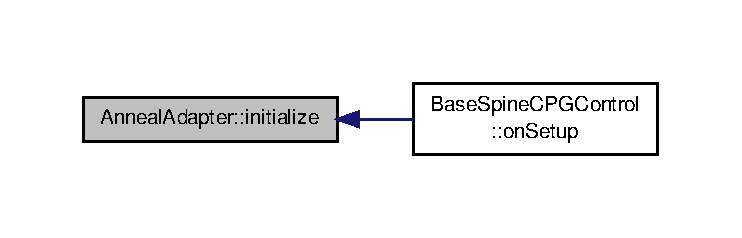
\includegraphics[width=350pt]{class_anneal_adapter_ac0ecb3b5380d94d99a8578297069f4bc_icgraph}
\end{center}
\end{figure}




The documentation for this class was generated from the following files\-:\begin{DoxyCompactItemize}
\item 
learning/\-Adapters/\hyperlink{_anneal_adapter_8h}{Anneal\-Adapter.\-h}\item 
learning/\-Adapters/\hyperlink{_anneal_adapter_8cpp}{Anneal\-Adapter.\-cpp}\end{DoxyCompactItemize}

\hypertarget{class_anneal_evolution}{\section{Anneal\-Evolution Class Reference}
\label{class_anneal_evolution}\index{Anneal\-Evolution@{Anneal\-Evolution}}
}
\subsection*{Public Member Functions}
\begin{DoxyCompactItemize}
\item 
\hypertarget{class_anneal_evolution_a3b76181520ac1449a1fbe302c83c5ef6}{{\bfseries Anneal\-Evolution} (string suffix, string config=\char`\"{}config.\-ini\char`\"{})}\label{class_anneal_evolution_a3b76181520ac1449a1fbe302c83c5ef6}

\item 
\hypertarget{class_anneal_evolution_acc1b2c6484762962eac3a8121c33990f}{void {\bfseries mutate\-Every\-Controller} ()}\label{class_anneal_evolution_acc1b2c6484762962eac3a8121c33990f}

\item 
\hypertarget{class_anneal_evolution_a54c20d2a6119dbca9ad65604cbc1d769}{void {\bfseries order\-All\-Populations} ()}\label{class_anneal_evolution_a54c20d2a6119dbca9ad65604cbc1d769}

\item 
\hypertarget{class_anneal_evolution_a49806407046d51576e508080baf956fd}{void {\bfseries evaluate\-Population} ()}\label{class_anneal_evolution_a49806407046d51576e508080baf956fd}

\item 
\hypertarget{class_anneal_evolution_a3e7a472b3cfbbedbf061648c186d46d9}{vector$<$ \hyperlink{class_anneal_evo_member}{Anneal\-Evo\-Member} $\ast$ $>$ {\bfseries next\-Set\-Of\-Controllers} ()}\label{class_anneal_evolution_a3e7a472b3cfbbedbf061648c186d46d9}

\item 
\hypertarget{class_anneal_evolution_a0d67a2b2103b4c6ce100da98553ca642}{void {\bfseries update\-Scores} (vector$<$ double $>$ scores)}\label{class_anneal_evolution_a0d67a2b2103b4c6ce100da98553ca642}

\end{DoxyCompactItemize}
\subsection*{Public Attributes}
\begin{DoxyCompactItemize}
\item 
\hypertarget{class_anneal_evolution_a97277a51ba42967c2cf479173543af7a}{string {\bfseries suffix}}\label{class_anneal_evolution_a97277a51ba42967c2cf479173543af7a}

\end{DoxyCompactItemize}


\subsection{Detailed Description}


Definition at line 43 of file Anneal\-Evolution.\-h.



The documentation for this class was generated from the following files\-:\begin{DoxyCompactItemize}
\item 
learning/\-Anneal\-Evolution/\hyperlink{_anneal_evolution_8h}{Anneal\-Evolution.\-h}\item 
learning/\-Anneal\-Evolution/\hyperlink{_anneal_evolution_8cpp}{Anneal\-Evolution.\-cpp}\end{DoxyCompactItemize}

\hypertarget{class_anneal_evo_member}{\section{Anneal\-Evo\-Member Class Reference}
\label{class_anneal_evo_member}\index{Anneal\-Evo\-Member@{Anneal\-Evo\-Member}}
}
\subsection*{Public Member Functions}
\begin{DoxyCompactItemize}
\item 
\hypertarget{class_anneal_evo_member_a1c0d923faddfb7b5228eb16b7107e916}{{\bfseries Anneal\-Evo\-Member} (\hyperlink{classconfiguration}{configuration} config)}\label{class_anneal_evo_member_a1c0d923faddfb7b5228eb16b7107e916}

\item 
\hypertarget{class_anneal_evo_member_a5d01b30e70e68731fdbb7196916a9f90}{void {\bfseries mutate} (std\-::tr1\-::ranlux64\-\_\-base\-\_\-01 $\ast$eng, double T)}\label{class_anneal_evo_member_a5d01b30e70e68731fdbb7196916a9f90}

\item 
\hypertarget{class_anneal_evo_member_aca0fda410629a7e291cf9639aafed305}{void {\bfseries copy\-From} (\hyperlink{class_anneal_evo_member}{Anneal\-Evo\-Member} $\ast$other\-Member)}\label{class_anneal_evo_member_aca0fda410629a7e291cf9639aafed305}

\item 
\hypertarget{class_anneal_evo_member_a8f90ad07fc150672328e9dfb92ce5478}{void {\bfseries save\-To\-File} (const char $\ast$output\-Filename)}\label{class_anneal_evo_member_a8f90ad07fc150672328e9dfb92ce5478}

\item 
\hypertarget{class_anneal_evo_member_ab246fd1e493ea859d79431f2658a89b8}{void {\bfseries load\-From\-File} (const char $\ast$input\-Filename)}\label{class_anneal_evo_member_ab246fd1e493ea859d79431f2658a89b8}

\end{DoxyCompactItemize}
\subsection*{Public Attributes}
\begin{DoxyCompactItemize}
\item 
\hypertarget{class_anneal_evo_member_abf9bffa087aa6c41375f7d1ef502170a}{vector$<$ double $>$ {\bfseries stateless\-Parameters}}\label{class_anneal_evo_member_abf9bffa087aa6c41375f7d1ef502170a}

\item 
\hypertarget{class_anneal_evo_member_a2b5dcacc081f1ea2ba2bafba95010a86}{vector$<$ double $>$ {\bfseries past\-Scores}}\label{class_anneal_evo_member_a2b5dcacc081f1ea2ba2bafba95010a86}

\item 
\hypertarget{class_anneal_evo_member_a3093f82effd3f947d2db9b09c5e5ed37}{double {\bfseries max\-Score}}\label{class_anneal_evo_member_a3093f82effd3f947d2db9b09c5e5ed37}

\item 
\hypertarget{class_anneal_evo_member_ad23339b2ffeb17f5daa3a82786087814}{double {\bfseries max\-Score1}}\label{class_anneal_evo_member_ad23339b2ffeb17f5daa3a82786087814}

\item 
\hypertarget{class_anneal_evo_member_a1de41ae7ca5d0763951807dc506ae9f5}{double {\bfseries max\-Score2}}\label{class_anneal_evo_member_a1de41ae7ca5d0763951807dc506ae9f5}

\item 
\hypertarget{class_anneal_evo_member_ac2acebeffb03591d4439ce6420691535}{double {\bfseries average\-Score}}\label{class_anneal_evo_member_ac2acebeffb03591d4439ce6420691535}

\end{DoxyCompactItemize}


\subsection{Detailed Description}


Definition at line 38 of file Anneal\-Evo\-Member.\-h.



The documentation for this class was generated from the following files\-:\begin{DoxyCompactItemize}
\item 
learning/\-Anneal\-Evolution/\hyperlink{_anneal_evo_member_8h}{Anneal\-Evo\-Member.\-h}\item 
learning/\-Anneal\-Evolution/\hyperlink{_anneal_evo_member_8cpp}{Anneal\-Evo\-Member.\-cpp}\end{DoxyCompactItemize}

\hypertarget{class_anneal_evo_population}{\section{Anneal\-Evo\-Population Class Reference}
\label{class_anneal_evo_population}\index{Anneal\-Evo\-Population@{Anneal\-Evo\-Population}}
}
\subsection*{Public Member Functions}
\begin{DoxyCompactItemize}
\item 
\hypertarget{class_anneal_evo_population_a5cd7269130339c2c150fb12610d2cd79}{{\bfseries Anneal\-Evo\-Population} (int num\-Controllers, \hyperlink{classconfiguration}{configuration} config)}\label{class_anneal_evo_population_a5cd7269130339c2c150fb12610d2cd79}

\item 
\hypertarget{class_anneal_evo_population_acb949779f11a27a5448746a078ec2d17}{void {\bfseries mutate} (std\-::tr1\-::ranlux64\-\_\-base\-\_\-01 $\ast$eng, int num\-To\-Mutate, double T)}\label{class_anneal_evo_population_acb949779f11a27a5448746a078ec2d17}

\item 
\hypertarget{class_anneal_evo_population_a188544d17492da2c8edbf4b7fb9b640f}{void {\bfseries order\-Population} ()}\label{class_anneal_evo_population_a188544d17492da2c8edbf4b7fb9b640f}

\item 
\hypertarget{class_anneal_evo_population_a974fdfab56b0b851cfe9b804c8b22e36}{\hyperlink{class_anneal_evo_member}{Anneal\-Evo\-Member} $\ast$ {\bfseries select\-Member\-To\-Evaluate} ()}\label{class_anneal_evo_population_a974fdfab56b0b851cfe9b804c8b22e36}

\item 
\hypertarget{class_anneal_evo_population_a73e97e2012f9b2cf7a109a247c77dd24}{\hyperlink{class_anneal_evo_member}{Anneal\-Evo\-Member} $\ast$ {\bfseries get\-Member} (int i)}\label{class_anneal_evo_population_a73e97e2012f9b2cf7a109a247c77dd24}

\end{DoxyCompactItemize}
\subsection*{Public Attributes}
\begin{DoxyCompactItemize}
\item 
\hypertarget{class_anneal_evo_population_aa1d274aa3646ed06e0ecca908315b526}{vector$<$ \hyperlink{class_anneal_evo_member}{Anneal\-Evo\-Member} $\ast$ $>$ {\bfseries controllers}}\label{class_anneal_evo_population_aa1d274aa3646ed06e0ecca908315b526}

\end{DoxyCompactItemize}


\subsection{Detailed Description}


Definition at line 34 of file Anneal\-Evo\-Population.\-h.



The documentation for this class was generated from the following files\-:\begin{DoxyCompactItemize}
\item 
learning/\-Anneal\-Evolution/\hyperlink{_anneal_evo_population_8h}{Anneal\-Evo\-Population.\-h}\item 
learning/\-Anneal\-Evolution/\hyperlink{_anneal_evo_population_8cpp}{Anneal\-Evo\-Population.\-cpp}\end{DoxyCompactItemize}

\hypertarget{class_base_spine_c_p_g_control}{\section{Base\-Spine\-C\-P\-G\-Control Class Reference}
\label{class_base_spine_c_p_g_control}\index{Base\-Spine\-C\-P\-G\-Control@{Base\-Spine\-C\-P\-G\-Control}}
}


Inheritance diagram for Base\-Spine\-C\-P\-G\-Control\-:\nopagebreak
\begin{figure}[H]
\begin{center}
\leavevmode
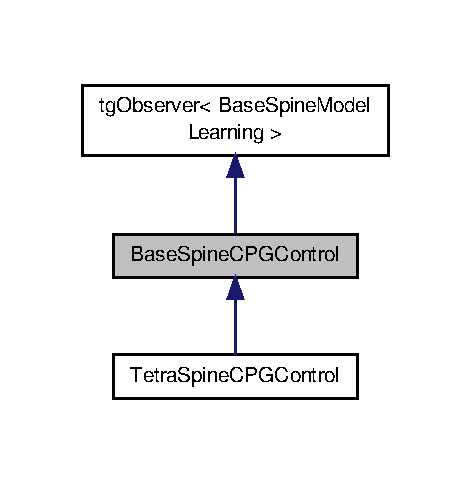
\includegraphics[width=226pt]{class_base_spine_c_p_g_control__inherit__graph}
\end{center}
\end{figure}


Collaboration diagram for Base\-Spine\-C\-P\-G\-Control\-:\nopagebreak
\begin{figure}[H]
\begin{center}
\leavevmode
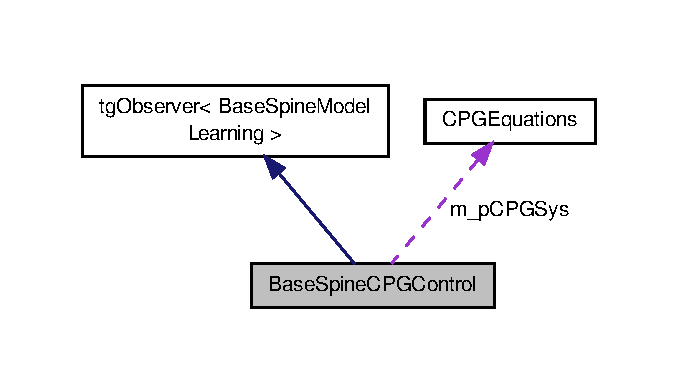
\includegraphics[width=326pt]{class_base_spine_c_p_g_control__coll__graph}
\end{center}
\end{figure}
\subsection*{Classes}
\begin{DoxyCompactItemize}
\item 
struct \hyperlink{struct_base_spine_c_p_g_control_1_1_config}{Config}
\end{DoxyCompactItemize}
\subsection*{Public Member Functions}
\begin{DoxyCompactItemize}
\item 
\hyperlink{class_base_spine_c_p_g_control_a8f7e5cb05f7285725b535e2ee8483faf}{Base\-Spine\-C\-P\-G\-Control} (\hyperlink{struct_base_spine_c_p_g_control_1_1_config}{Base\-Spine\-C\-P\-G\-Control\-::\-Config} config, std\-::string args, std\-::string ec=\char`\"{}edge\-Config.\-ini\char`\"{}, std\-::string nc=\char`\"{}node\-Config.\-ini\char`\"{})
\item 
virtual void \hyperlink{class_base_spine_c_p_g_control_afa0b0e1f995545476511eac4fd322da2}{on\-Step} (\hyperlink{class_base_spine_model_learning}{Base\-Spine\-Model\-Learning} \&subject, double dt)
\item 
virtual void \hyperlink{class_base_spine_c_p_g_control_a25508234dbe960a6fea460d2abd6f353}{on\-Setup} (\hyperlink{class_base_spine_model_learning}{Base\-Spine\-Model\-Learning} \&subject)
\item 
virtual void \hyperlink{class_base_spine_c_p_g_control_aa209e0699b3dfc5889c6084409be4d20}{on\-Teardown} (\hyperlink{class_base_spine_model_learning}{Base\-Spine\-Model\-Learning} \&subject)
\item 
virtual void \hyperlink{classtg_observer_a0ecd07483eb41f9a0ab19b8ed24052f1}{on\-Attach} (\hyperlink{class_base_spine_model_learning}{Base\-Spine\-Model\-Learning} \&subject)
\end{DoxyCompactItemize}
\subsection*{Protected Member Functions}
\begin{DoxyCompactItemize}
\item 
virtual array\-\_\-4\-D \hyperlink{class_base_spine_c_p_g_control_afe859425b72dcacf780647676571045b}{scale\-Edge\-Actions} (std\-::vector$<$ std\-::vector$<$ double $>$ $>$ actions)
\item 
\hypertarget{class_base_spine_c_p_g_control_a69503b94c6783d03efcfc962c4dc8c92}{virtual array\-\_\-2\-D {\bfseries scale\-Node\-Actions} (std\-::vector$<$ std\-::vector$<$ double $>$ $>$ actions)}\label{class_base_spine_c_p_g_control_a69503b94c6783d03efcfc962c4dc8c92}

\item 
virtual void \hyperlink{class_base_spine_c_p_g_control_a4f54eecdac3f19693752a77a8668f119}{setup\-C\-P\-Gs} (\hyperlink{class_base_spine_model_learning}{Base\-Spine\-Model\-Learning} \&subject, array\-\_\-2\-D node\-Actions, array\-\_\-4\-D edge\-Actions)
\end{DoxyCompactItemize}
\subsection*{Protected Attributes}
\begin{DoxyCompactItemize}
\item 
\hypertarget{class_base_spine_c_p_g_control_ae6746549e7b65841996fef5702c91292}{\hyperlink{class_c_p_g_equations}{C\-P\-G\-Equations} $\ast$ {\bfseries m\-\_\-p\-C\-P\-G\-Sys}}\label{class_base_spine_c_p_g_control_ae6746549e7b65841996fef5702c91292}

\item 
\hypertarget{class_base_spine_c_p_g_control_a2b440435221a786a5f6576ad993d3aac}{std\-::vector$<$ \hyperlink{classtg_c_p_g_string_control}{tg\-C\-P\-G\-String\-Control} $\ast$ $>$ {\bfseries m\-\_\-all\-Controllers}}\label{class_base_spine_c_p_g_control_a2b440435221a786a5f6576ad993d3aac}

\end{DoxyCompactItemize}


\subsection{Detailed Description}


Definition at line 43 of file Base\-Spine\-C\-P\-G\-Control.\-h.



\subsection{Constructor \& Destructor Documentation}
\hypertarget{class_base_spine_c_p_g_control_a8f7e5cb05f7285725b535e2ee8483faf}{\index{Base\-Spine\-C\-P\-G\-Control@{Base\-Spine\-C\-P\-G\-Control}!Base\-Spine\-C\-P\-G\-Control@{Base\-Spine\-C\-P\-G\-Control}}
\index{Base\-Spine\-C\-P\-G\-Control@{Base\-Spine\-C\-P\-G\-Control}!BaseSpineCPGControl@{Base\-Spine\-C\-P\-G\-Control}}
\subsubsection[{Base\-Spine\-C\-P\-G\-Control}]{\setlength{\rightskip}{0pt plus 5cm}Base\-Spine\-C\-P\-G\-Control\-::\-Base\-Spine\-C\-P\-G\-Control (
\begin{DoxyParamCaption}
\item[{{\bf Base\-Spine\-C\-P\-G\-Control\-::\-Config}}]{config, }
\item[{std\-::string}]{args, }
\item[{std\-::string}]{ec = {\ttfamily \char`\"{}edgeConfig.ini\char`\"{}}, }
\item[{std\-::string}]{nc = {\ttfamily \char`\"{}nodeConfig.ini\char`\"{}}}
\end{DoxyParamCaption}
)}}\label{class_base_spine_c_p_g_control_a8f7e5cb05f7285725b535e2ee8483faf}
Defining the adapters here assumes the controller is around and attached for the lifecycle of the learning runs. I.\-E. that the setup and teardown functions are used for \hyperlink{classtg_model}{tg\-Model} 

Definition at line 116 of file Base\-Spine\-C\-P\-G\-Control.\-cpp.



\subsection{Member Function Documentation}
\hypertarget{classtg_observer_a0ecd07483eb41f9a0ab19b8ed24052f1}{\index{Base\-Spine\-C\-P\-G\-Control@{Base\-Spine\-C\-P\-G\-Control}!on\-Attach@{on\-Attach}}
\index{on\-Attach@{on\-Attach}!BaseSpineCPGControl@{Base\-Spine\-C\-P\-G\-Control}}
\subsubsection[{on\-Attach}]{\setlength{\rightskip}{0pt plus 5cm}virtual void {\bf tg\-Observer}$<$ {\bf Base\-Spine\-Model\-Learning}  $>$\-::on\-Attach (
\begin{DoxyParamCaption}
\item[{{\bf Base\-Spine\-Model\-Learning}  \&}]{subject}
\end{DoxyParamCaption}
)\hspace{0.3cm}{\ttfamily [inline]}, {\ttfamily [virtual]}, {\ttfamily [inherited]}}}\label{classtg_observer_a0ecd07483eb41f9a0ab19b8ed24052f1}
Notify the observers when an attach action has occurred. Will only occur once, typically before setup 
\begin{DoxyParams}[1]{Parameters}
\mbox{\tt in,out}  & {\em subject} & the subject being observed \\
\hline
\end{DoxyParams}


Definition at line 54 of file tg\-Observer.\-h.

\hypertarget{class_base_spine_c_p_g_control_a25508234dbe960a6fea460d2abd6f353}{\index{Base\-Spine\-C\-P\-G\-Control@{Base\-Spine\-C\-P\-G\-Control}!on\-Setup@{on\-Setup}}
\index{on\-Setup@{on\-Setup}!BaseSpineCPGControl@{Base\-Spine\-C\-P\-G\-Control}}
\subsubsection[{on\-Setup}]{\setlength{\rightskip}{0pt plus 5cm}void Base\-Spine\-C\-P\-G\-Control\-::on\-Setup (
\begin{DoxyParamCaption}
\item[{{\bf Base\-Spine\-Model\-Learning} \&}]{subject}
\end{DoxyParamCaption}
)\hspace{0.3cm}{\ttfamily [virtual]}}}\label{class_base_spine_c_p_g_control_a25508234dbe960a6fea460d2abd6f353}
Notify the observers when a setup action has occurred. 
\begin{DoxyParams}[1]{Parameters}
\mbox{\tt in,out}  & {\em subject} & the subject being observed \\
\hline
\end{DoxyParams}


Reimplemented from \hyperlink{classtg_observer_ae7b2de87bd4a6e786bc16f1b801c36a6}{tg\-Observer$<$ Base\-Spine\-Model\-Learning $>$}.



Definition at line 140 of file Base\-Spine\-C\-P\-G\-Control.\-cpp.

\hypertarget{class_base_spine_c_p_g_control_afa0b0e1f995545476511eac4fd322da2}{\index{Base\-Spine\-C\-P\-G\-Control@{Base\-Spine\-C\-P\-G\-Control}!on\-Step@{on\-Step}}
\index{on\-Step@{on\-Step}!BaseSpineCPGControl@{Base\-Spine\-C\-P\-G\-Control}}
\subsubsection[{on\-Step}]{\setlength{\rightskip}{0pt plus 5cm}void Base\-Spine\-C\-P\-G\-Control\-::on\-Step (
\begin{DoxyParamCaption}
\item[{{\bf Base\-Spine\-Model\-Learning} \&}]{subject, }
\item[{double}]{dt}
\end{DoxyParamCaption}
)\hspace{0.3cm}{\ttfamily [virtual]}}}\label{class_base_spine_c_p_g_control_afa0b0e1f995545476511eac4fd322da2}
Notify the observers when a step action has occurred. 
\begin{DoxyParams}[1]{Parameters}
\mbox{\tt in,out}  & {\em subject} & the subject being observed \\
\hline
\mbox{\tt in}  & {\em the} & number of seconds since the previous call; must be positive \\
\hline
\end{DoxyParams}


Implements \hyperlink{classtg_observer_a6db5ef1e2792102b8e36dbad5e1a3d7a}{tg\-Observer$<$ Base\-Spine\-Model\-Learning $>$}.



Definition at line 215 of file Base\-Spine\-C\-P\-G\-Control.\-cpp.



Here is the call graph for this function\-:\nopagebreak
\begin{figure}[H]
\begin{center}
\leavevmode
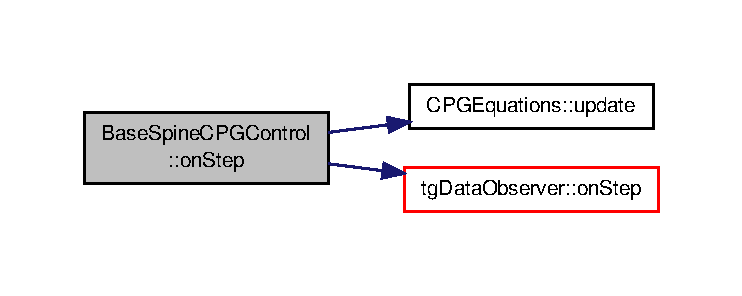
\includegraphics[width=350pt]{class_base_spine_c_p_g_control_afa0b0e1f995545476511eac4fd322da2_cgraph}
\end{center}
\end{figure}


\hypertarget{class_base_spine_c_p_g_control_aa209e0699b3dfc5889c6084409be4d20}{\index{Base\-Spine\-C\-P\-G\-Control@{Base\-Spine\-C\-P\-G\-Control}!on\-Teardown@{on\-Teardown}}
\index{on\-Teardown@{on\-Teardown}!BaseSpineCPGControl@{Base\-Spine\-C\-P\-G\-Control}}
\subsubsection[{on\-Teardown}]{\setlength{\rightskip}{0pt plus 5cm}void Base\-Spine\-C\-P\-G\-Control\-::on\-Teardown (
\begin{DoxyParamCaption}
\item[{{\bf Base\-Spine\-Model\-Learning} \&}]{subject}
\end{DoxyParamCaption}
)\hspace{0.3cm}{\ttfamily [virtual]}}}\label{class_base_spine_c_p_g_control_aa209e0699b3dfc5889c6084409be4d20}
Notify the observers when a teardown action has occurred. 
\begin{DoxyParams}[1]{Parameters}
\mbox{\tt in,out}  & {\em subject} & the subject being observed \\
\hline
\end{DoxyParams}
\begin{DoxyRefDesc}{Todo}
\item[\hyperlink{todo__todo000031}{Todo}]
\begin{DoxyItemize}
\item consolidate with other controller classes. 
\end{DoxyItemize}\end{DoxyRefDesc}
\begin{DoxyRefDesc}{Todo}
\item[\hyperlink{todo__todo000032}{Todo}]
\begin{DoxyItemize}
\item return length scale as a parameter 
\end{DoxyItemize}\end{DoxyRefDesc}


Reimplemented from \hyperlink{classtg_observer_a1663edb3732e5ffb7bbe6bfb4ade88b8}{tg\-Observer$<$ Base\-Spine\-Model\-Learning $>$}.



Definition at line 233 of file Base\-Spine\-C\-P\-G\-Control.\-cpp.

\hypertarget{class_base_spine_c_p_g_control_afe859425b72dcacf780647676571045b}{\index{Base\-Spine\-C\-P\-G\-Control@{Base\-Spine\-C\-P\-G\-Control}!scale\-Edge\-Actions@{scale\-Edge\-Actions}}
\index{scale\-Edge\-Actions@{scale\-Edge\-Actions}!BaseSpineCPGControl@{Base\-Spine\-C\-P\-G\-Control}}
\subsubsection[{scale\-Edge\-Actions}]{\setlength{\rightskip}{0pt plus 5cm}array\-\_\-4\-D Base\-Spine\-C\-P\-G\-Control\-::scale\-Edge\-Actions (
\begin{DoxyParamCaption}
\item[{std\-::vector$<$ std\-::vector$<$ double $>$ $>$}]{actions}
\end{DoxyParamCaption}
)\hspace{0.3cm}{\ttfamily [protected]}, {\ttfamily [virtual]}}}\label{class_base_spine_c_p_g_control_afe859425b72dcacf780647676571045b}
Takes a vector of parameters reported by learning, and then converts it into a format used to assign to the C\-P\-G\-Edges Note that if the C\-P\-G edges change, this will need to change 

Definition at line 289 of file Base\-Spine\-C\-P\-G\-Control.\-cpp.



Here is the caller graph for this function\-:\nopagebreak
\begin{figure}[H]
\begin{center}
\leavevmode
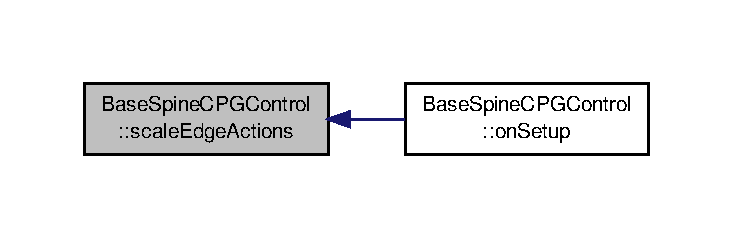
\includegraphics[width=350pt]{class_base_spine_c_p_g_control_afe859425b72dcacf780647676571045b_icgraph}
\end{center}
\end{figure}


\hypertarget{class_base_spine_c_p_g_control_a4f54eecdac3f19693752a77a8668f119}{\index{Base\-Spine\-C\-P\-G\-Control@{Base\-Spine\-C\-P\-G\-Control}!setup\-C\-P\-Gs@{setup\-C\-P\-Gs}}
\index{setup\-C\-P\-Gs@{setup\-C\-P\-Gs}!BaseSpineCPGControl@{Base\-Spine\-C\-P\-G\-Control}}
\subsubsection[{setup\-C\-P\-Gs}]{\setlength{\rightskip}{0pt plus 5cm}void Base\-Spine\-C\-P\-G\-Control\-::setup\-C\-P\-Gs (
\begin{DoxyParamCaption}
\item[{{\bf Base\-Spine\-Model\-Learning} \&}]{subject, }
\item[{array\-\_\-2\-D}]{node\-Actions, }
\item[{array\-\_\-4\-D}]{edge\-Actions}
\end{DoxyParamCaption}
)\hspace{0.3cm}{\ttfamily [protected]}, {\ttfamily [virtual]}}}\label{class_base_spine_c_p_g_control_a4f54eecdac3f19693752a77a8668f119}
\begin{DoxyRefDesc}{Todo}
\item[\hyperlink{todo__todo000030}{Todo}]\-: redo with for\-\_\-each \end{DoxyRefDesc}


Reimplemented in \hyperlink{class_tetra_spine_c_p_g_control_a1011f7ba6c6df843b8a7d3bd64f75ac5}{Tetra\-Spine\-C\-P\-G\-Control}.



Definition at line 173 of file Base\-Spine\-C\-P\-G\-Control.\-cpp.



Here is the call graph for this function\-:\nopagebreak
\begin{figure}[H]
\begin{center}
\leavevmode
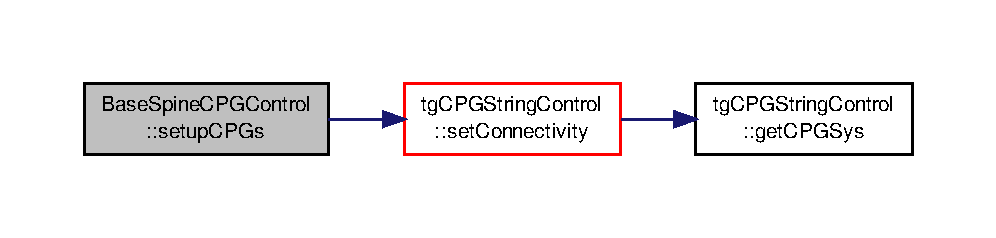
\includegraphics[width=350pt]{class_base_spine_c_p_g_control_a4f54eecdac3f19693752a77a8668f119_cgraph}
\end{center}
\end{figure}




Here is the caller graph for this function\-:\nopagebreak
\begin{figure}[H]
\begin{center}
\leavevmode
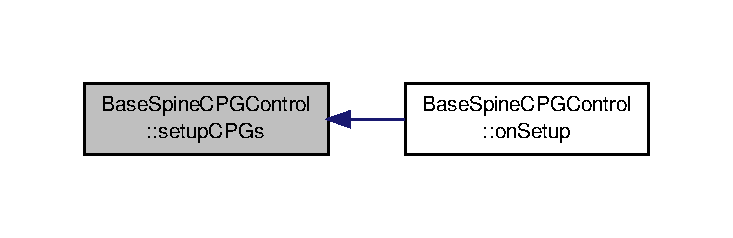
\includegraphics[width=350pt]{class_base_spine_c_p_g_control_a4f54eecdac3f19693752a77a8668f119_icgraph}
\end{center}
\end{figure}




The documentation for this class was generated from the following files\-:\begin{DoxyCompactItemize}
\item 
dev/btietz/Base\-Spine\-C\-P\-G\-Control.\-h\item 
dev/btietz/Base\-Spine\-C\-P\-G\-Control.\-cpp\end{DoxyCompactItemize}

\hypertarget{class_base_spine_model_learning}{\section{Base\-Spine\-Model\-Learning Class Reference}
\label{class_base_spine_model_learning}\index{Base\-Spine\-Model\-Learning@{Base\-Spine\-Model\-Learning}}
}


Inherits \hyperlink{classtg_subject}{tg\-Subject$<$ Base\-Spine\-Model\-Learning $>$}, and \hyperlink{classtg_model}{tg\-Model}.



Inherited by \hyperlink{class_flemons_spine_model_learning}{Flemons\-Spine\-Model\-Learning}, \hyperlink{class_flemons_spine_model_learning}{Flemons\-Spine\-Model\-Learning}, \hyperlink{class_rib_model}{Rib\-Model}, and \hyperlink{class_tetra_spine_learning_model}{Tetra\-Spine\-Learning\-Model}.



Collaboration diagram for Base\-Spine\-Model\-Learning\-:\nopagebreak
\begin{figure}[H]
\begin{center}
\leavevmode
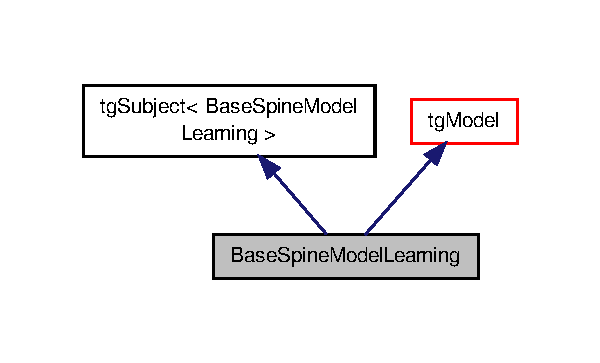
\includegraphics[width=288pt]{class_base_spine_model_learning__coll__graph}
\end{center}
\end{figure}
\subsection*{Public Types}
\begin{DoxyCompactItemize}
\item 
\hypertarget{class_base_spine_model_learning_a0f779ad979f0353d68af012f50f822b7}{typedef std\-::map$<$ std\-::string, \\*
std\-::vector$<$ \hyperlink{classtg_linear_string}{tg\-Linear\-String} $\ast$ $>$ $>$ {\bfseries Muscle\-Map}}\label{class_base_spine_model_learning_a0f779ad979f0353d68af012f50f822b7}

\end{DoxyCompactItemize}
\subsection*{Public Member Functions}
\begin{DoxyCompactItemize}
\item 
virtual void \hyperlink{class_base_spine_model_learning_a6d97d4097674fb9c7ea7f667e11442bb}{setup} (\hyperlink{classtg_world}{tg\-World} \&world)
\item 
virtual void \hyperlink{class_base_spine_model_learning_aa04ab240035720769a95c403c1f61f73}{teardown} ()
\item 
virtual void \hyperlink{class_base_spine_model_learning_abe197971d9b438aaaf36d2e8bddfc739}{step} (double dt)
\item 
\hypertarget{class_base_spine_model_learning_afd3d71b99a2105a60c78d52d67068c00}{virtual std\-::vector$<$ double $>$ {\bfseries get\-Segment\-C\-O\-M} (const int n) const }\label{class_base_spine_model_learning_afd3d71b99a2105a60c78d52d67068c00}

\item 
\hypertarget{class_base_spine_model_learning_a0c595346fb7a23e89d9f6ec572a19c49}{virtual const std\-::vector\\*
$<$ \hyperlink{classtg_linear_string}{tg\-Linear\-String} $\ast$ $>$ \& {\bfseries get\-Muscles} (const std\-::string \&key) const }\label{class_base_spine_model_learning_a0c595346fb7a23e89d9f6ec572a19c49}

\item 
\hypertarget{class_base_spine_model_learning_a508eae423b9fd9e194b620563b15b9db}{virtual const std\-::vector\\*
$<$ \hyperlink{classtg_linear_string}{tg\-Linear\-String} $\ast$ $>$ \& {\bfseries get\-All\-Muscles} ()}\label{class_base_spine_model_learning_a508eae423b9fd9e194b620563b15b9db}

\item 
\hypertarget{class_base_spine_model_learning_af38ddf518f0b9d524d869591216070fd}{virtual const int {\bfseries get\-Segments} ()}\label{class_base_spine_model_learning_af38ddf518f0b9d524d869591216070fd}

\item 
\hypertarget{class_base_spine_model_learning_a21c0b6e4c84e4f61b92d803dd677525f}{virtual std\-::size\-\_\-t {\bfseries get\-Numberof\-Muslces} () const }\label{class_base_spine_model_learning_a21c0b6e4c84e4f61b92d803dd677525f}

\item 
void \hyperlink{classtg_subject_a56ecfd33a048c3a7f1a884318d9af548}{attach} (\hyperlink{classtg_observer}{tg\-Observer}$<$ \hyperlink{class_base_spine_model_learning}{Base\-Spine\-Model\-Learning} $>$ $\ast$p\-Observer)
\item 
void \hyperlink{classtg_subject_ad9640aa7fcc1e0b4ce8a913a4ce1ea42}{notify\-Step} (double dt)
\item 
void \hyperlink{classtg_subject_a80799e5d0c8512d3d05a55764790392b}{notify\-Setup} ()
\item 
void \hyperlink{classtg_subject_adf7a60dbb0faf0de5528f862e7953e63}{notify\-Teardown} ()
\item 
virtual void \hyperlink{classtg_model_aee6457e0fc54d5570b87bfc779f9b1c0}{on\-Visit} (const \hyperlink{classtg_model_visitor}{tg\-Model\-Visitor} \&r) const 
\item 
void \hyperlink{classtg_model_a292c17848b96caee32b2286e44c13f2f}{add\-Child} (\hyperlink{classtg_model}{tg\-Model} $\ast$p\-Child)
\item 
virtual std\-::string \hyperlink{classtg_model_af37b0c1a6d4060bfe0bb9b5038a17725}{to\-String} (std\-::string prefix=\char`\"{}\char`\"{}) const 
\item 
{\footnotesize template$<$typename T $>$ }\\std\-::vector$<$ T $\ast$ $>$ \hyperlink{classtg_model_ab75836fdfbd9200f165c3b28a19630c0}{find} (const \hyperlink{classtg_tag_search}{tg\-Tag\-Search} \&tag\-Search)
\item 
{\footnotesize template$<$typename T $>$ }\\std\-::vector$<$ T $\ast$ $>$ \hyperlink{classtg_model_aa40b5fb32f8941e04d537f4e6c6db35c}{find} (const std\-::string \&tag\-Search)
\item 
std\-::vector$<$ \hyperlink{classtg_model}{tg\-Model} $\ast$ $>$ \hyperlink{classtg_model_a2efa4321fa5c77b4ce23b01f6fd3a1c4}{get\-Descendants} () const 
\item 
\hypertarget{classtg_taggable_af0b8f1729653b0b90d2fecbd51163612}{void {\bfseries add\-Tags} (const std\-::string \&space\-\_\-separated\-\_\-tags)}\label{classtg_taggable_af0b8f1729653b0b90d2fecbd51163612}

\item 
\hypertarget{classtg_taggable_af28e3fe1a7e4eb28772dc006d575dd1f}{void {\bfseries add\-Tags} (const \hyperlink{classtg_tags}{tg\-Tags} \&tags)}\label{classtg_taggable_af28e3fe1a7e4eb28772dc006d575dd1f}

\item 
\hypertarget{classtg_taggable_ae31f65869c8887bfeb34a344902c4d5b}{bool {\bfseries has\-Tag} (const std\-::string tag) const }\label{classtg_taggable_ae31f65869c8887bfeb34a344902c4d5b}

\item 
\hypertarget{classtg_taggable_a33b77b1075171b63f673965687b2e844}{bool {\bfseries has\-All\-Tags} (std\-::string tags)}\label{classtg_taggable_a33b77b1075171b63f673965687b2e844}

\item 
\hypertarget{classtg_taggable_af14af28fa98021c4f20a5e8f2ddd5606}{bool {\bfseries has\-Any\-Tags} (const std\-::string tags)}\label{classtg_taggable_af14af28fa98021c4f20a5e8f2ddd5606}

\item 
\hypertarget{classtg_taggable_adff345e116e16420c701a748ff8f995f}{bool {\bfseries has\-No\-Tags} ()}\label{classtg_taggable_adff345e116e16420c701a748ff8f995f}

\item 
\hypertarget{classtg_taggable_acf1d7fa9df8f374f25015c4080902681}{\hyperlink{classtg_tags}{tg\-Tags} \& {\bfseries get\-Tags} ()}\label{classtg_taggable_acf1d7fa9df8f374f25015c4080902681}

\item 
\hypertarget{classtg_taggable_ae70d7d3b45301665bc363b0ed8b9b292}{const \hyperlink{classtg_tags}{tg\-Tags} \& {\bfseries get\-Tags} () const }\label{classtg_taggable_ae70d7d3b45301665bc363b0ed8b9b292}

\item 
\hypertarget{classtg_taggable_a5492888e4e4da4cca6261070b5726adf}{void {\bfseries set\-Tags} (\hyperlink{classtg_tags}{tg\-Tags} tags)}\label{classtg_taggable_a5492888e4e4da4cca6261070b5726adf}

\item 
\hypertarget{classtg_taggable_a346d66b066d2d9eb1eadba01da43749f}{std\-::string {\bfseries get\-Tag\-Str} (std\-::string delim=\char`\"{} \char`\"{}) const }\label{classtg_taggable_a346d66b066d2d9eb1eadba01da43749f}

\end{DoxyCompactItemize}
\subsection*{Protected Member Functions}
\begin{DoxyCompactItemize}
\item 
\hypertarget{class_base_spine_model_learning_a666bf86f666e0830c6b2da7f5176e750}{{\bfseries Base\-Spine\-Model\-Learning} (int segments)}\label{class_base_spine_model_learning_a666bf86f666e0830c6b2da7f5176e750}

\end{DoxyCompactItemize}
\subsection*{Protected Attributes}
\begin{DoxyCompactItemize}
\item 
\hypertarget{class_base_spine_model_learning_a9cd74c4c79da8749fb5c8bffecede666}{std\-::vector$<$ \hyperlink{classtg_linear_string}{tg\-Linear\-String} $\ast$ $>$ {\bfseries m\-\_\-all\-Muscles}}\label{class_base_spine_model_learning_a9cd74c4c79da8749fb5c8bffecede666}

\item 
\hypertarget{class_base_spine_model_learning_a1c1e64b40b4c67189fbc67ad411f316a}{std\-::vector$<$ \hyperlink{classtg_model}{tg\-Model} $\ast$ $>$ {\bfseries m\-\_\-all\-Segments}}\label{class_base_spine_model_learning_a1c1e64b40b4c67189fbc67ad411f316a}

\item 
\hypertarget{class_base_spine_model_learning_a75cad2ae3b68f93d283550b417af5523}{Muscle\-Map {\bfseries m\-\_\-muscle\-Map}}\label{class_base_spine_model_learning_a75cad2ae3b68f93d283550b417af5523}

\item 
\hypertarget{class_base_spine_model_learning_a5d68dbbcbda4091b040279200a185d50}{const std\-::size\-\_\-t {\bfseries m\-\_\-segments}}\label{class_base_spine_model_learning_a5d68dbbcbda4091b040279200a185d50}

\end{DoxyCompactItemize}


\subsection{Detailed Description}


Definition at line 35 of file Base\-Spine\-Model\-Learning.\-h.



\subsection{Member Function Documentation}
\hypertarget{classtg_model_a292c17848b96caee32b2286e44c13f2f}{\index{Base\-Spine\-Model\-Learning@{Base\-Spine\-Model\-Learning}!add\-Child@{add\-Child}}
\index{add\-Child@{add\-Child}!BaseSpineModelLearning@{Base\-Spine\-Model\-Learning}}
\subsubsection[{add\-Child}]{\setlength{\rightskip}{0pt plus 5cm}void tg\-Model\-::add\-Child (
\begin{DoxyParamCaption}
\item[{{\bf tg\-Model} $\ast$}]{p\-Child}
\end{DoxyParamCaption}
)\hspace{0.3cm}{\ttfamily [inherited]}}}\label{classtg_model_a292c17848b96caee32b2286e44c13f2f}
Add a sub-\/model to this model. The model takes ownership of the child sub-\/model and is responsible for deallocating it. 
\begin{DoxyParams}[1]{Parameters}
\mbox{\tt in,out}  & {\em p\-Child} & a pointer to a sub-\/model \\
\hline
\end{DoxyParams}

\begin{DoxyExceptions}{Exceptions}
{\em std\-::invalid\-\_\-argument} & is p\-Child is N\-U\-L\-L, this object, or already a descendant \\
\hline
\end{DoxyExceptions}
\begin{DoxyRefDesc}{Todo}
\item[\hyperlink{todo__todo000016}{Todo}]Make sure that every child appears no more than once in the tree. \end{DoxyRefDesc}


Definition at line 126 of file tg\-Model.\-cpp.



Here is the call graph for this function\-:\nopagebreak
\begin{figure}[H]
\begin{center}
\leavevmode
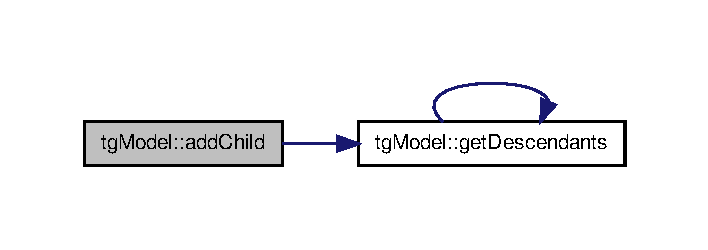
\includegraphics[width=340pt]{classtg_model_a292c17848b96caee32b2286e44c13f2f_cgraph}
\end{center}
\end{figure}




Here is the caller graph for this function\-:\nopagebreak
\begin{figure}[H]
\begin{center}
\leavevmode
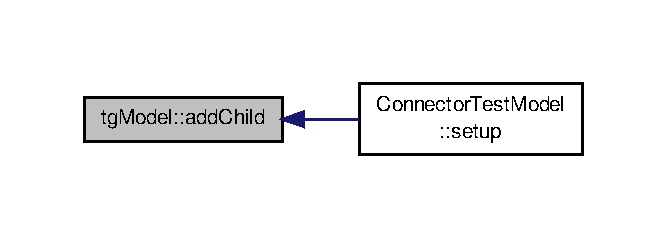
\includegraphics[width=320pt]{classtg_model_a292c17848b96caee32b2286e44c13f2f_icgraph}
\end{center}
\end{figure}


\hypertarget{classtg_subject_a56ecfd33a048c3a7f1a884318d9af548}{\index{Base\-Spine\-Model\-Learning@{Base\-Spine\-Model\-Learning}!attach@{attach}}
\index{attach@{attach}!BaseSpineModelLearning@{Base\-Spine\-Model\-Learning}}
\subsubsection[{attach}]{\setlength{\rightskip}{0pt plus 5cm}void {\bf tg\-Subject}$<$ {\bf Base\-Spine\-Model\-Learning}  $>$\-::attach (
\begin{DoxyParamCaption}
\item[{{\bf tg\-Observer}$<$ {\bf Base\-Spine\-Model\-Learning}  $>$ $\ast$}]{p\-Observer}
\end{DoxyParamCaption}
)\hspace{0.3cm}{\ttfamily [inherited]}}}\label{classtg_subject_a56ecfd33a048c3a7f1a884318d9af548}
Attach an observer to the subject of the observer. 
\begin{DoxyParams}[1]{Parameters}
\mbox{\tt in,out}  & {\em p\-Observer} & a pointer to an observer for the subject; do nothing if the pointer is N\-U\-L\-L \\
\hline
\end{DoxyParams}
\hypertarget{classtg_model_ab75836fdfbd9200f165c3b28a19630c0}{\index{Base\-Spine\-Model\-Learning@{Base\-Spine\-Model\-Learning}!find@{find}}
\index{find@{find}!BaseSpineModelLearning@{Base\-Spine\-Model\-Learning}}
\subsubsection[{find}]{\setlength{\rightskip}{0pt plus 5cm}template$<$typename T $>$ std\-::vector$<$T$\ast$$>$ tg\-Model\-::find (
\begin{DoxyParamCaption}
\item[{const {\bf tg\-Tag\-Search} \&}]{tag\-Search}
\end{DoxyParamCaption}
)\hspace{0.3cm}{\ttfamily [inline]}, {\ttfamily [inherited]}}}\label{classtg_model_ab75836fdfbd9200f165c3b28a19630c0}
Get a vector of descendants sorted by type and a tagsearch. Useful for pulling out muscle groups, or similar. 
\begin{DoxyParams}[1]{Parameters}
\mbox{\tt in}  & {\em tag\-Search,a} & tag\-Search that contains the desired tags \\
\hline
\end{DoxyParams}
\begin{DoxyReturn}{Returns}
a std\-::vector of pointers to members that match the tag search and typename T 
\end{DoxyReturn}


Definition at line 129 of file tg\-Model.\-h.



Here is the call graph for this function\-:\nopagebreak
\begin{figure}[H]
\begin{center}
\leavevmode
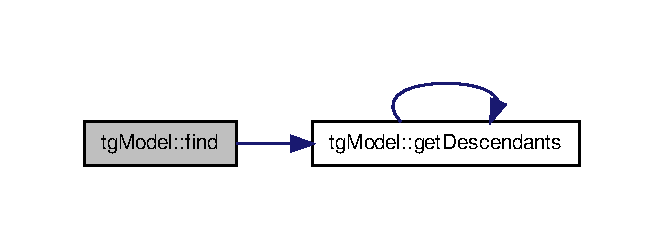
\includegraphics[width=318pt]{classtg_model_ab75836fdfbd9200f165c3b28a19630c0_cgraph}
\end{center}
\end{figure}


\hypertarget{classtg_model_aa40b5fb32f8941e04d537f4e6c6db35c}{\index{Base\-Spine\-Model\-Learning@{Base\-Spine\-Model\-Learning}!find@{find}}
\index{find@{find}!BaseSpineModelLearning@{Base\-Spine\-Model\-Learning}}
\subsubsection[{find}]{\setlength{\rightskip}{0pt plus 5cm}template$<$typename T $>$ std\-::vector$<$T$\ast$$>$ tg\-Model\-::find (
\begin{DoxyParamCaption}
\item[{const std\-::string \&}]{tag\-Search}
\end{DoxyParamCaption}
)\hspace{0.3cm}{\ttfamily [inline]}, {\ttfamily [inherited]}}}\label{classtg_model_aa40b5fb32f8941e04d537f4e6c6db35c}
Get a vector of descendants sorted by type and a tagsearch. Useful for pulling out muscle groups, or similar. 
\begin{DoxyParams}[1]{Parameters}
\mbox{\tt in}  & {\em tag\-Search,a} & std\-::string\& that contains the desired tags \\
\hline
\end{DoxyParams}
\begin{DoxyReturn}{Returns}
a std\-::vector of pointers to members that match the tag search and typename T 
\end{DoxyReturn}


Definition at line 142 of file tg\-Model.\-h.



Here is the call graph for this function\-:\nopagebreak
\begin{figure}[H]
\begin{center}
\leavevmode
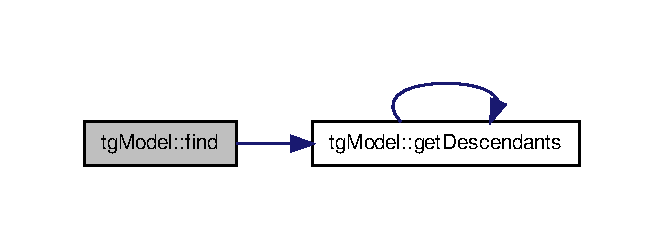
\includegraphics[width=318pt]{classtg_model_aa40b5fb32f8941e04d537f4e6c6db35c_cgraph}
\end{center}
\end{figure}


\hypertarget{classtg_model_a2efa4321fa5c77b4ce23b01f6fd3a1c4}{\index{Base\-Spine\-Model\-Learning@{Base\-Spine\-Model\-Learning}!get\-Descendants@{get\-Descendants}}
\index{get\-Descendants@{get\-Descendants}!BaseSpineModelLearning@{Base\-Spine\-Model\-Learning}}
\subsubsection[{get\-Descendants}]{\setlength{\rightskip}{0pt plus 5cm}std\-::vector$<$ {\bf tg\-Model} $\ast$ $>$ tg\-Model\-::get\-Descendants (
\begin{DoxyParamCaption}
{}
\end{DoxyParamCaption}
) const\hspace{0.3cm}{\ttfamily [inherited]}}}\label{classtg_model_a2efa4321fa5c77b4ce23b01f6fd3a1c4}
Return a std\-::vector of const pointers to all sub-\/models. \begin{DoxyRefDesc}{Todo}
\item[\hyperlink{todo__todo000017}{Todo}]examine whether this should be public, and perhaps create a read only version \end{DoxyRefDesc}
\begin{DoxyReturn}{Returns}
a std\-::vector of const pointers all sub-\/models.
\end{DoxyReturn}
\begin{DoxyRefDesc}{Todo}
\item[\hyperlink{todo__todo000014}{Todo}]Unnecessary copying can be avoided by pasing the result collection in the recursive step. \end{DoxyRefDesc}


Definition at line 174 of file tg\-Model.\-cpp.



Here is the call graph for this function\-:\nopagebreak
\begin{figure}[H]
\begin{center}
\leavevmode
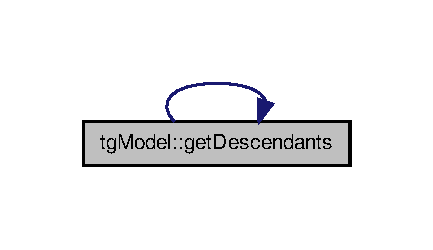
\includegraphics[width=208pt]{classtg_model_a2efa4321fa5c77b4ce23b01f6fd3a1c4_cgraph}
\end{center}
\end{figure}


\hypertarget{classtg_subject_a80799e5d0c8512d3d05a55764790392b}{\index{Base\-Spine\-Model\-Learning@{Base\-Spine\-Model\-Learning}!notify\-Setup@{notify\-Setup}}
\index{notify\-Setup@{notify\-Setup}!BaseSpineModelLearning@{Base\-Spine\-Model\-Learning}}
\subsubsection[{notify\-Setup}]{\setlength{\rightskip}{0pt plus 5cm}void {\bf tg\-Subject}$<$ {\bf Base\-Spine\-Model\-Learning}  $>$\-::notify\-Setup (
\begin{DoxyParamCaption}
{}
\end{DoxyParamCaption}
)\hspace{0.3cm}{\ttfamily [inherited]}}}\label{classtg_subject_a80799e5d0c8512d3d05a55764790392b}
Call \hyperlink{classtg_observer_ae7b2de87bd4a6e786bc16f1b801c36a6}{tg\-Observer$<$\-T$>$\-::on\-Setup()} on all observers in the order in which they were attached. \hypertarget{classtg_subject_ad9640aa7fcc1e0b4ce8a913a4ce1ea42}{\index{Base\-Spine\-Model\-Learning@{Base\-Spine\-Model\-Learning}!notify\-Step@{notify\-Step}}
\index{notify\-Step@{notify\-Step}!BaseSpineModelLearning@{Base\-Spine\-Model\-Learning}}
\subsubsection[{notify\-Step}]{\setlength{\rightskip}{0pt plus 5cm}void {\bf tg\-Subject}$<$ {\bf Base\-Spine\-Model\-Learning}  $>$\-::notify\-Step (
\begin{DoxyParamCaption}
\item[{double}]{dt}
\end{DoxyParamCaption}
)\hspace{0.3cm}{\ttfamily [inherited]}}}\label{classtg_subject_ad9640aa7fcc1e0b4ce8a913a4ce1ea42}
Call \hyperlink{classtg_observer_a6db5ef1e2792102b8e36dbad5e1a3d7a}{tg\-Observer$<$\-T$>$\-::on\-Step()} on all observers in the order in which they were attached. 
\begin{DoxyParams}[1]{Parameters}
\mbox{\tt in}  & {\em dt} & the number of seconds since the previous call; do nothing if not positive \\
\hline
\end{DoxyParams}
\hypertarget{classtg_subject_adf7a60dbb0faf0de5528f862e7953e63}{\index{Base\-Spine\-Model\-Learning@{Base\-Spine\-Model\-Learning}!notify\-Teardown@{notify\-Teardown}}
\index{notify\-Teardown@{notify\-Teardown}!BaseSpineModelLearning@{Base\-Spine\-Model\-Learning}}
\subsubsection[{notify\-Teardown}]{\setlength{\rightskip}{0pt plus 5cm}void {\bf tg\-Subject}$<$ {\bf Base\-Spine\-Model\-Learning}  $>$\-::notify\-Teardown (
\begin{DoxyParamCaption}
{}
\end{DoxyParamCaption}
)\hspace{0.3cm}{\ttfamily [inherited]}}}\label{classtg_subject_adf7a60dbb0faf0de5528f862e7953e63}
Call \hyperlink{classtg_observer_a1663edb3732e5ffb7bbe6bfb4ade88b8}{tg\-Observer$<$\-T$>$\-::on\-Teardown()} on all observers in the order in which they were attached. \hypertarget{classtg_model_aee6457e0fc54d5570b87bfc779f9b1c0}{\index{Base\-Spine\-Model\-Learning@{Base\-Spine\-Model\-Learning}!on\-Visit@{on\-Visit}}
\index{on\-Visit@{on\-Visit}!BaseSpineModelLearning@{Base\-Spine\-Model\-Learning}}
\subsubsection[{on\-Visit}]{\setlength{\rightskip}{0pt plus 5cm}void tg\-Model\-::on\-Visit (
\begin{DoxyParamCaption}
\item[{const {\bf tg\-Model\-Visitor} \&}]{r}
\end{DoxyParamCaption}
) const\hspace{0.3cm}{\ttfamily [virtual]}, {\ttfamily [inherited]}}}\label{classtg_model_aee6457e0fc54d5570b87bfc779f9b1c0}
Call \hyperlink{classtg_model_visitor_a69d056cf31bb4eeef03c243a86f59cc1}{tg\-Model\-Visitor\-::render()} on self and all descendants. 
\begin{DoxyParams}[1]{Parameters}
\mbox{\tt in,out}  & {\em r} & a reference to a \hyperlink{classtg_model_visitor}{tg\-Model\-Visitor} \\
\hline
\end{DoxyParams}


Reimplemented in \hyperlink{class_connector_test_model_a8d4e146eb48dd23676a5522e9417abdb}{Connector\-Test\-Model}, \hyperlink{class_build_test_model_a8f12c5e787faba7606bbd46531819a4b}{Build\-Test\-Model}, \hyperlink{classtg_linear_string_a9f659486ba4276dc9d60982158fb7aa5}{tg\-Linear\-String}, and \hyperlink{classtg_rod_ae3651ef650b66a5d016bc5ffb27ec449}{tg\-Rod}.



Definition at line 109 of file tg\-Model.\-cpp.



Here is the call graph for this function\-:\nopagebreak
\begin{figure}[H]
\begin{center}
\leavevmode
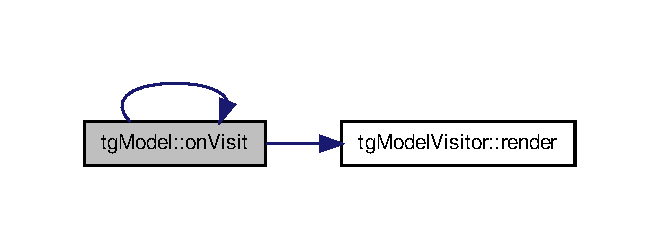
\includegraphics[width=316pt]{classtg_model_aee6457e0fc54d5570b87bfc779f9b1c0_cgraph}
\end{center}
\end{figure}


\hypertarget{class_base_spine_model_learning_a6d97d4097674fb9c7ea7f667e11442bb}{\index{Base\-Spine\-Model\-Learning@{Base\-Spine\-Model\-Learning}!setup@{setup}}
\index{setup@{setup}!BaseSpineModelLearning@{Base\-Spine\-Model\-Learning}}
\subsubsection[{setup}]{\setlength{\rightskip}{0pt plus 5cm}void Base\-Spine\-Model\-Learning\-::setup (
\begin{DoxyParamCaption}
\item[{{\bf tg\-World} \&}]{world}
\end{DoxyParamCaption}
)\hspace{0.3cm}{\ttfamily [virtual]}}}\label{class_base_spine_model_learning_a6d97d4097674fb9c7ea7f667e11442bb}
Setup takes a \hyperlink{classtg_world}{tg\-World} and passes it to any children for their own setup functions. All subclasses should call this at the appropriate time (usually end of setup) within their own setup function. 
\begin{DoxyParams}[1]{Parameters}
\mbox{\tt in}  & {\em world} & -\/ the \hyperlink{classtg_world}{tg\-World} the models will exist in. \\
\hline
\end{DoxyParams}


Reimplemented from \hyperlink{classtg_model_a85c68e064972f67c61c47ead392cf6f8}{tg\-Model}.



Reimplemented in \hyperlink{class_flemons_spine_model_learning_ad7d329634cf8d812bcee974a3430fcee}{Flemons\-Spine\-Model\-Learning}, \hyperlink{class_flemons_spine_model_learning_a1c5e086a665023dbc637cfd617ddc094}{Flemons\-Spine\-Model\-Learning}, \hyperlink{class_tetra_spine_learning_model_a78f283f3a2479c9af5b43cef52f2428f}{Tetra\-Spine\-Learning\-Model}, and \hyperlink{class_rib_model_a4cbc6a0649ca5deb7ab0c98b8ae1ab1e}{Rib\-Model}.



Definition at line 49 of file Base\-Spine\-Model\-Learning.\-cpp.



Here is the call graph for this function\-:\nopagebreak
\begin{figure}[H]
\begin{center}
\leavevmode
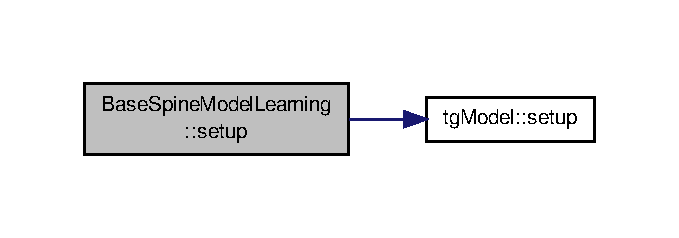
\includegraphics[width=326pt]{class_base_spine_model_learning_a6d97d4097674fb9c7ea7f667e11442bb_cgraph}
\end{center}
\end{figure}


\hypertarget{class_base_spine_model_learning_abe197971d9b438aaaf36d2e8bddfc739}{\index{Base\-Spine\-Model\-Learning@{Base\-Spine\-Model\-Learning}!step@{step}}
\index{step@{step}!BaseSpineModelLearning@{Base\-Spine\-Model\-Learning}}
\subsubsection[{step}]{\setlength{\rightskip}{0pt plus 5cm}void Base\-Spine\-Model\-Learning\-::step (
\begin{DoxyParamCaption}
\item[{double}]{dt}
\end{DoxyParamCaption}
)\hspace{0.3cm}{\ttfamily [virtual]}}}\label{class_base_spine_model_learning_abe197971d9b438aaaf36d2e8bddfc739}
Advance the simulation. 
\begin{DoxyParams}[1]{Parameters}
\mbox{\tt in}  & {\em dt} & the number of seconds since the previous call; std\-::invalid\-\_\-argument is thrown if dt is not positive \\
\hline
\end{DoxyParams}

\begin{DoxyExceptions}{Exceptions}
{\em std\-::invalid\-\_\-argument} & if dt is not positive \\
\hline
\end{DoxyExceptions}
\begin{DoxyNote}{Note}
This is not necessarily const for every child. 
\end{DoxyNote}


Reimplemented from \hyperlink{classtg_model_acc6f9ae005f9f51447d7efe5f1815737}{tg\-Model}.



Reimplemented in \hyperlink{class_flemons_spine_model_learning_ab0c5bc7a89e7358015877ed147b66da9}{Flemons\-Spine\-Model\-Learning}, \hyperlink{class_flemons_spine_model_learning_a29969832ceaa6143afcce7dfe1d6d8e8}{Flemons\-Spine\-Model\-Learning}, \hyperlink{class_tetra_spine_learning_model_a5b3b6e1543c56deafe50d7cf3478ebfe}{Tetra\-Spine\-Learning\-Model}, and \hyperlink{class_rib_model_a71a67cc85f18bf8bf72c82b3e7d8c538}{Rib\-Model}.



Definition at line 70 of file Base\-Spine\-Model\-Learning.\-cpp.



Here is the call graph for this function\-:\nopagebreak
\begin{figure}[H]
\begin{center}
\leavevmode
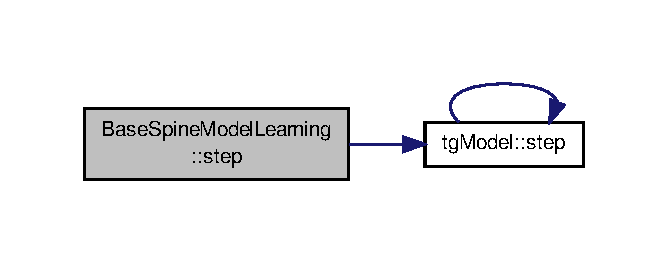
\includegraphics[width=320pt]{class_base_spine_model_learning_abe197971d9b438aaaf36d2e8bddfc739_cgraph}
\end{center}
\end{figure}


\hypertarget{class_base_spine_model_learning_aa04ab240035720769a95c403c1f61f73}{\index{Base\-Spine\-Model\-Learning@{Base\-Spine\-Model\-Learning}!teardown@{teardown}}
\index{teardown@{teardown}!BaseSpineModelLearning@{Base\-Spine\-Model\-Learning}}
\subsubsection[{teardown}]{\setlength{\rightskip}{0pt plus 5cm}void Base\-Spine\-Model\-Learning\-::teardown (
\begin{DoxyParamCaption}
{}
\end{DoxyParamCaption}
)\hspace{0.3cm}{\ttfamily [virtual]}}}\label{class_base_spine_model_learning_aa04ab240035720769a95c403c1f61f73}
Deletes the children (undoes setup) 

Reimplemented from \hyperlink{classtg_model_adb5eec1dcf70a8c039850aea144dcc7e}{tg\-Model}.



Reimplemented in \hyperlink{class_flemons_spine_model_learning_a489aeb8529c20f9a2473812ea0e78f41}{Flemons\-Spine\-Model\-Learning}, \hyperlink{class_flemons_spine_model_learning_ab2f98f3230f4980bed706d9337a2fae5}{Flemons\-Spine\-Model\-Learning}, \hyperlink{class_tetra_spine_learning_model_a242f0c007fb565c278a26b4efcc299f4}{Tetra\-Spine\-Learning\-Model}, and \hyperlink{class_rib_model_a1f44d22a7213cd3042383c56dcbac61f}{Rib\-Model}.



Definition at line 58 of file Base\-Spine\-Model\-Learning.\-cpp.



Here is the call graph for this function\-:\nopagebreak
\begin{figure}[H]
\begin{center}
\leavevmode
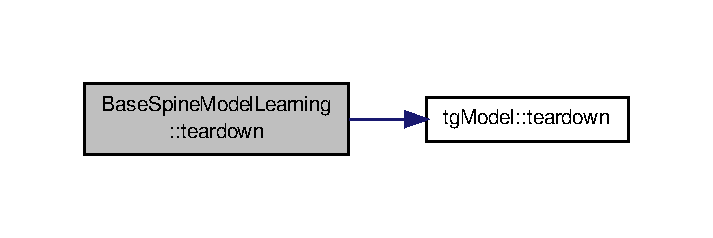
\includegraphics[width=342pt]{class_base_spine_model_learning_aa04ab240035720769a95c403c1f61f73_cgraph}
\end{center}
\end{figure}


\hypertarget{classtg_model_af37b0c1a6d4060bfe0bb9b5038a17725}{\index{Base\-Spine\-Model\-Learning@{Base\-Spine\-Model\-Learning}!to\-String@{to\-String}}
\index{to\-String@{to\-String}!BaseSpineModelLearning@{Base\-Spine\-Model\-Learning}}
\subsubsection[{to\-String}]{\setlength{\rightskip}{0pt plus 5cm}std\-::string tg\-Model\-::to\-String (
\begin{DoxyParamCaption}
\item[{std\-::string}]{prefix = {\ttfamily \char`\"{}\char`\"{}}}
\end{DoxyParamCaption}
) const\hspace{0.3cm}{\ttfamily [virtual]}, {\ttfamily [inherited]}}}\label{classtg_model_af37b0c1a6d4060bfe0bb9b5038a17725}
Returns the tag names of this model and its children 
\begin{DoxyParams}[1]{Parameters}
\mbox{\tt in}  & {\em prefix} & a string to append to \\
\hline
\end{DoxyParams}
\begin{DoxyReturn}{Returns}
the original string with this model and its children's tags appended 
\end{DoxyReturn}


Definition at line 156 of file tg\-Model.\-cpp.



Here is the caller graph for this function\-:\nopagebreak
\begin{figure}[H]
\begin{center}
\leavevmode
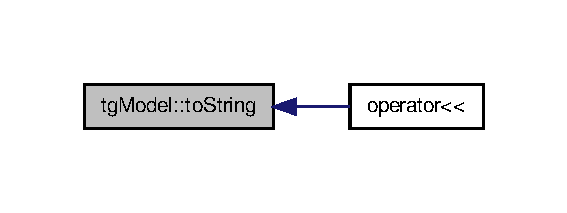
\includegraphics[width=272pt]{classtg_model_af37b0c1a6d4060bfe0bb9b5038a17725_icgraph}
\end{center}
\end{figure}




The documentation for this class was generated from the following files\-:\begin{DoxyCompactItemize}
\item 
dev/btietz/Base\-Spine\-Model\-Learning.\-h\item 
dev/btietz/Base\-Spine\-Model\-Learning.\-cpp\end{DoxyCompactItemize}

\hypertarget{structtg_base_string_1_1_base_string_history}{\section{tg\-Base\-String\-:\-:Base\-String\-History Struct Reference}
\label{structtg_base_string_1_1_base_string_history}\index{tg\-Base\-String\-::\-Base\-String\-History@{tg\-Base\-String\-::\-Base\-String\-History}}
}


{\ttfamily \#include $<$tg\-Base\-String.\-h$>$}

\subsection*{Public Attributes}
\begin{DoxyCompactItemize}
\item 
std\-::deque$<$ double $>$ \hyperlink{structtg_base_string_1_1_base_string_history_a9cb214114d51a5c43bbe820b0ebea690}{last\-Lengths}
\item 
std\-::deque$<$ double $>$ \hyperlink{structtg_base_string_1_1_base_string_history_aba048e0d7ddad106779a8f76fe8ccb0e}{rest\-Lengths}
\item 
std\-::deque$<$ double $>$ \hyperlink{structtg_base_string_1_1_base_string_history_a45f7d448b2c9dd487d47782f09822449}{damping\-History}
\item 
std\-::deque$<$ double $>$ \hyperlink{structtg_base_string_1_1_base_string_history_ae084154b0fccaafadeacf1f246f22115}{last\-Velocities}
\item 
std\-::deque$<$ double $>$ \hyperlink{structtg_base_string_1_1_base_string_history_a7488efc0119d4d2abeff29fc52606340}{tension\-History}
\end{DoxyCompactItemize}


\subsection{Detailed Description}
Encapsulate the history members. 

Definition at line 150 of file tg\-Base\-String.\-h.



\subsection{Member Data Documentation}
\hypertarget{structtg_base_string_1_1_base_string_history_a45f7d448b2c9dd487d47782f09822449}{\index{tg\-Base\-String\-::\-Base\-String\-History@{tg\-Base\-String\-::\-Base\-String\-History}!damping\-History@{damping\-History}}
\index{damping\-History@{damping\-History}!tgBaseString::BaseStringHistory@{tg\-Base\-String\-::\-Base\-String\-History}}
\subsubsection[{damping\-History}]{\setlength{\rightskip}{0pt plus 5cm}std\-::deque$<$double$>$ tg\-Base\-String\-::\-Base\-String\-History\-::damping\-History}}\label{structtg_base_string_1_1_base_string_history_a45f7d448b2c9dd487d47782f09822449}
Damping history. 

Definition at line 159 of file tg\-Base\-String.\-h.

\hypertarget{structtg_base_string_1_1_base_string_history_a9cb214114d51a5c43bbe820b0ebea690}{\index{tg\-Base\-String\-::\-Base\-String\-History@{tg\-Base\-String\-::\-Base\-String\-History}!last\-Lengths@{last\-Lengths}}
\index{last\-Lengths@{last\-Lengths}!tgBaseString::BaseStringHistory@{tg\-Base\-String\-::\-Base\-String\-History}}
\subsubsection[{last\-Lengths}]{\setlength{\rightskip}{0pt plus 5cm}std\-::deque$<$double$>$ tg\-Base\-String\-::\-Base\-String\-History\-::last\-Lengths}}\label{structtg_base_string_1_1_base_string_history_a9cb214114d51a5c43bbe820b0ebea690}
Length history. 

Definition at line 153 of file tg\-Base\-String.\-h.

\hypertarget{structtg_base_string_1_1_base_string_history_ae084154b0fccaafadeacf1f246f22115}{\index{tg\-Base\-String\-::\-Base\-String\-History@{tg\-Base\-String\-::\-Base\-String\-History}!last\-Velocities@{last\-Velocities}}
\index{last\-Velocities@{last\-Velocities}!tgBaseString::BaseStringHistory@{tg\-Base\-String\-::\-Base\-String\-History}}
\subsubsection[{last\-Velocities}]{\setlength{\rightskip}{0pt plus 5cm}std\-::deque$<$double$>$ tg\-Base\-String\-::\-Base\-String\-History\-::last\-Velocities}}\label{structtg_base_string_1_1_base_string_history_ae084154b0fccaafadeacf1f246f22115}
Velocity history. 

Definition at line 162 of file tg\-Base\-String.\-h.

\hypertarget{structtg_base_string_1_1_base_string_history_aba048e0d7ddad106779a8f76fe8ccb0e}{\index{tg\-Base\-String\-::\-Base\-String\-History@{tg\-Base\-String\-::\-Base\-String\-History}!rest\-Lengths@{rest\-Lengths}}
\index{rest\-Lengths@{rest\-Lengths}!tgBaseString::BaseStringHistory@{tg\-Base\-String\-::\-Base\-String\-History}}
\subsubsection[{rest\-Lengths}]{\setlength{\rightskip}{0pt plus 5cm}std\-::deque$<$double$>$ tg\-Base\-String\-::\-Base\-String\-History\-::rest\-Lengths}}\label{structtg_base_string_1_1_base_string_history_aba048e0d7ddad106779a8f76fe8ccb0e}
Rest length history. 

Definition at line 156 of file tg\-Base\-String.\-h.

\hypertarget{structtg_base_string_1_1_base_string_history_a7488efc0119d4d2abeff29fc52606340}{\index{tg\-Base\-String\-::\-Base\-String\-History@{tg\-Base\-String\-::\-Base\-String\-History}!tension\-History@{tension\-History}}
\index{tension\-History@{tension\-History}!tgBaseString::BaseStringHistory@{tg\-Base\-String\-::\-Base\-String\-History}}
\subsubsection[{tension\-History}]{\setlength{\rightskip}{0pt plus 5cm}std\-::deque$<$double$>$ tg\-Base\-String\-::\-Base\-String\-History\-::tension\-History}}\label{structtg_base_string_1_1_base_string_history_a7488efc0119d4d2abeff29fc52606340}
Tension history. 

Definition at line 165 of file tg\-Base\-String.\-h.



The documentation for this struct was generated from the following file\-:\begin{DoxyCompactItemize}
\item 
core/\hyperlink{tg_base_string_8h}{tg\-Base\-String.\-h}\end{DoxyCompactItemize}

\hypertarget{class_build_test_controller}{\section{Build\-Test\-Controller Class Reference}
\label{class_build_test_controller}\index{Build\-Test\-Controller@{Build\-Test\-Controller}}
}


Inheritance diagram for Build\-Test\-Controller\-:\nopagebreak
\begin{figure}[H]
\begin{center}
\leavevmode
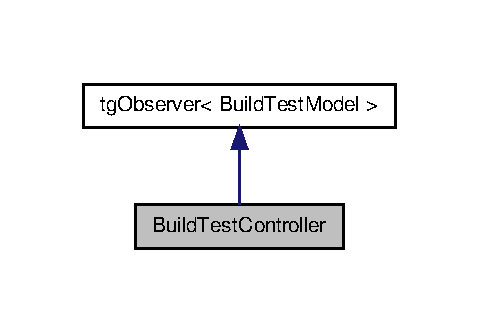
\includegraphics[width=230pt]{class_build_test_controller__inherit__graph}
\end{center}
\end{figure}


Collaboration diagram for Build\-Test\-Controller\-:\nopagebreak
\begin{figure}[H]
\begin{center}
\leavevmode
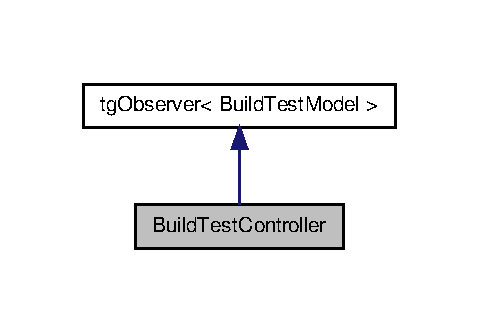
\includegraphics[width=230pt]{class_build_test_controller__coll__graph}
\end{center}
\end{figure}
\subsection*{Public Member Functions}
\begin{DoxyCompactItemize}
\item 
void \hyperlink{class_build_test_controller_a8eba0a685d2e8b499591841effd085b8}{on\-Step} (\hyperlink{class_build_test_model}{Build\-Test\-Model} \&model, double dt)
\item 
virtual void \hyperlink{classtg_observer_a0ecd07483eb41f9a0ab19b8ed24052f1}{on\-Attach} (\hyperlink{class_build_test_model}{Build\-Test\-Model} \&subject)
\item 
virtual void \hyperlink{classtg_observer_ae7b2de87bd4a6e786bc16f1b801c36a6}{on\-Setup} (\hyperlink{class_build_test_model}{Build\-Test\-Model} \&subject)
\item 
virtual void \hyperlink{classtg_observer_a1663edb3732e5ffb7bbe6bfb4ade88b8}{on\-Teardown} (\hyperlink{class_build_test_model}{Build\-Test\-Model} \&subject)
\end{DoxyCompactItemize}


\subsection{Detailed Description}


Definition at line 21 of file Build\-Test\-Controller.\-h.



\subsection{Member Function Documentation}
\hypertarget{classtg_observer_a0ecd07483eb41f9a0ab19b8ed24052f1}{\index{Build\-Test\-Controller@{Build\-Test\-Controller}!on\-Attach@{on\-Attach}}
\index{on\-Attach@{on\-Attach}!BuildTestController@{Build\-Test\-Controller}}
\subsubsection[{on\-Attach}]{\setlength{\rightskip}{0pt plus 5cm}virtual void {\bf tg\-Observer}$<$ {\bf Build\-Test\-Model}  $>$\-::on\-Attach (
\begin{DoxyParamCaption}
\item[{{\bf Build\-Test\-Model}  \&}]{subject}
\end{DoxyParamCaption}
)\hspace{0.3cm}{\ttfamily [inline]}, {\ttfamily [virtual]}, {\ttfamily [inherited]}}}\label{classtg_observer_a0ecd07483eb41f9a0ab19b8ed24052f1}
Notify the observers when an attach action has occurred. Will only occur once, typically before setup 
\begin{DoxyParams}[1]{Parameters}
\mbox{\tt in,out}  & {\em subject} & the subject being observed \\
\hline
\end{DoxyParams}


Definition at line 54 of file tg\-Observer.\-h.

\hypertarget{classtg_observer_ae7b2de87bd4a6e786bc16f1b801c36a6}{\index{Build\-Test\-Controller@{Build\-Test\-Controller}!on\-Setup@{on\-Setup}}
\index{on\-Setup@{on\-Setup}!BuildTestController@{Build\-Test\-Controller}}
\subsubsection[{on\-Setup}]{\setlength{\rightskip}{0pt plus 5cm}virtual void {\bf tg\-Observer}$<$ {\bf Build\-Test\-Model}  $>$\-::on\-Setup (
\begin{DoxyParamCaption}
\item[{{\bf Build\-Test\-Model}  \&}]{subject}
\end{DoxyParamCaption}
)\hspace{0.3cm}{\ttfamily [inline]}, {\ttfamily [virtual]}, {\ttfamily [inherited]}}}\label{classtg_observer_ae7b2de87bd4a6e786bc16f1b801c36a6}
Notify the observers when a setup action has occurred. 
\begin{DoxyParams}[1]{Parameters}
\mbox{\tt in,out}  & {\em subject} & the subject being observed \\
\hline
\end{DoxyParams}


Definition at line 60 of file tg\-Observer.\-h.

\hypertarget{class_build_test_controller_a8eba0a685d2e8b499591841effd085b8}{\index{Build\-Test\-Controller@{Build\-Test\-Controller}!on\-Step@{on\-Step}}
\index{on\-Step@{on\-Step}!BuildTestController@{Build\-Test\-Controller}}
\subsubsection[{on\-Step}]{\setlength{\rightskip}{0pt plus 5cm}void Build\-Test\-Controller\-::on\-Step (
\begin{DoxyParamCaption}
\item[{{\bf Build\-Test\-Model} \&}]{subject, }
\item[{double}]{dt}
\end{DoxyParamCaption}
)\hspace{0.3cm}{\ttfamily [inline]}, {\ttfamily [virtual]}}}\label{class_build_test_controller_a8eba0a685d2e8b499591841effd085b8}
Notify the observers when a step action has occurred. 
\begin{DoxyParams}[1]{Parameters}
\mbox{\tt in,out}  & {\em subject} & the subject being observed \\
\hline
\mbox{\tt in}  & {\em the} & number of seconds since the previous call; must be positive \\
\hline
\end{DoxyParams}


Implements \hyperlink{classtg_observer_a6db5ef1e2792102b8e36dbad5e1a3d7a}{tg\-Observer$<$ Build\-Test\-Model $>$}.



Definition at line 24 of file Build\-Test\-Controller.\-h.

\hypertarget{classtg_observer_a1663edb3732e5ffb7bbe6bfb4ade88b8}{\index{Build\-Test\-Controller@{Build\-Test\-Controller}!on\-Teardown@{on\-Teardown}}
\index{on\-Teardown@{on\-Teardown}!BuildTestController@{Build\-Test\-Controller}}
\subsubsection[{on\-Teardown}]{\setlength{\rightskip}{0pt plus 5cm}virtual void {\bf tg\-Observer}$<$ {\bf Build\-Test\-Model}  $>$\-::on\-Teardown (
\begin{DoxyParamCaption}
\item[{{\bf Build\-Test\-Model}  \&}]{subject}
\end{DoxyParamCaption}
)\hspace{0.3cm}{\ttfamily [inline]}, {\ttfamily [virtual]}, {\ttfamily [inherited]}}}\label{classtg_observer_a1663edb3732e5ffb7bbe6bfb4ade88b8}
Notify the observers when a teardown action has occurred. 
\begin{DoxyParams}[1]{Parameters}
\mbox{\tt in,out}  & {\em subject} & the subject being observed \\
\hline
\end{DoxyParams}


Definition at line 66 of file tg\-Observer.\-h.



The documentation for this class was generated from the following file\-:\begin{DoxyCompactItemize}
\item 
dev/tests/Build\-Test\-Controller.\-h\end{DoxyCompactItemize}

\hypertarget{class_build_test_model}{\section{Build\-Test\-Model Class Reference}
\label{class_build_test_model}\index{Build\-Test\-Model@{Build\-Test\-Model}}
}


Inheritance diagram for Build\-Test\-Model\-:\nopagebreak
\begin{figure}[H]
\begin{center}
\leavevmode
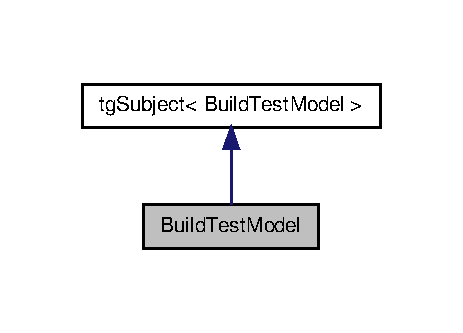
\includegraphics[width=222pt]{class_build_test_model__inherit__graph}
\end{center}
\end{figure}


Collaboration diagram for Build\-Test\-Model\-:\nopagebreak
\begin{figure}[H]
\begin{center}
\leavevmode
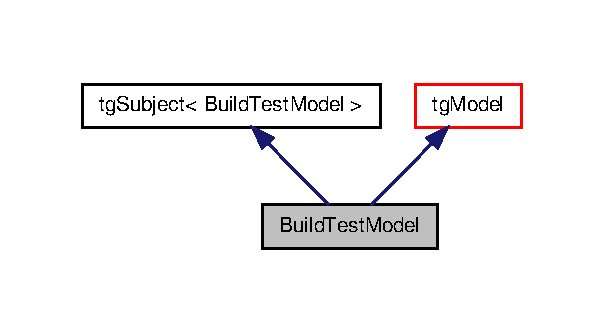
\includegraphics[width=290pt]{class_build_test_model__coll__graph}
\end{center}
\end{figure}
\subsection*{Public Member Functions}
\begin{DoxyCompactItemize}
\item 
\hypertarget{class_build_test_model_ae18318d9e981ffb33a337bd5b2372f16}{{\bfseries Build\-Test\-Model} (std\-::string name)}\label{class_build_test_model_ae18318d9e981ffb33a337bd5b2372f16}

\item 
virtual void \hyperlink{class_build_test_model_ac41e963bca43e2bc670e18f0801671f7}{setup} (\hyperlink{classtg_world}{tg\-World} \&world)
\item 
virtual void \hyperlink{class_build_test_model_aabd9261840e8466e8648585ccca67397}{step} (double dt)
\item 
virtual void \hyperlink{class_build_test_model_a8f12c5e787faba7606bbd46531819a4b}{on\-Visit} (const \hyperlink{classtg_model_visitor}{tg\-Model\-Visitor} \&r) const 
\item 
\hypertarget{class_build_test_model_a7ac393b0062ec64141a6938f5295d2e9}{void {\bfseries change\-Muscle} (double length)}\label{class_build_test_model_a7ac393b0062ec64141a6938f5295d2e9}

\item 
void \hyperlink{classtg_subject_a56ecfd33a048c3a7f1a884318d9af548}{attach} (\hyperlink{classtg_observer}{tg\-Observer}$<$ \hyperlink{class_build_test_model}{Build\-Test\-Model} $>$ $\ast$p\-Observer)
\item 
void \hyperlink{classtg_subject_ad9640aa7fcc1e0b4ce8a913a4ce1ea42}{notify\-Step} (double dt)
\item 
void \hyperlink{classtg_subject_a80799e5d0c8512d3d05a55764790392b}{notify\-Setup} ()
\item 
void \hyperlink{classtg_subject_adf7a60dbb0faf0de5528f862e7953e63}{notify\-Teardown} ()
\item 
virtual void \hyperlink{classtg_model_adb5eec1dcf70a8c039850aea144dcc7e}{teardown} ()
\item 
void \hyperlink{classtg_model_a292c17848b96caee32b2286e44c13f2f}{add\-Child} (\hyperlink{classtg_model}{tg\-Model} $\ast$p\-Child)
\item 
virtual std\-::string \hyperlink{classtg_model_af37b0c1a6d4060bfe0bb9b5038a17725}{to\-String} (std\-::string prefix=\char`\"{}\char`\"{}) const 
\item 
{\footnotesize template$<$typename T $>$ }\\std\-::vector$<$ T $\ast$ $>$ \hyperlink{classtg_model_ab75836fdfbd9200f165c3b28a19630c0}{find} (const \hyperlink{classtg_tag_search}{tg\-Tag\-Search} \&tag\-Search)
\item 
{\footnotesize template$<$typename T $>$ }\\std\-::vector$<$ T $\ast$ $>$ \hyperlink{classtg_model_aa40b5fb32f8941e04d537f4e6c6db35c}{find} (const std\-::string \&tag\-Search)
\item 
std\-::vector$<$ \hyperlink{classtg_model}{tg\-Model} $\ast$ $>$ \hyperlink{classtg_model_a2efa4321fa5c77b4ce23b01f6fd3a1c4}{get\-Descendants} () const 
\item 
\hypertarget{classtg_taggable_af0b8f1729653b0b90d2fecbd51163612}{void {\bfseries add\-Tags} (const std\-::string \&space\-\_\-separated\-\_\-tags)}\label{classtg_taggable_af0b8f1729653b0b90d2fecbd51163612}

\item 
\hypertarget{classtg_taggable_af28e3fe1a7e4eb28772dc006d575dd1f}{void {\bfseries add\-Tags} (const \hyperlink{classtg_tags}{tg\-Tags} \&tags)}\label{classtg_taggable_af28e3fe1a7e4eb28772dc006d575dd1f}

\item 
\hypertarget{classtg_taggable_ae31f65869c8887bfeb34a344902c4d5b}{bool {\bfseries has\-Tag} (const std\-::string tag) const }\label{classtg_taggable_ae31f65869c8887bfeb34a344902c4d5b}

\item 
\hypertarget{classtg_taggable_a33b77b1075171b63f673965687b2e844}{bool {\bfseries has\-All\-Tags} (std\-::string tags)}\label{classtg_taggable_a33b77b1075171b63f673965687b2e844}

\item 
\hypertarget{classtg_taggable_af14af28fa98021c4f20a5e8f2ddd5606}{bool {\bfseries has\-Any\-Tags} (const std\-::string tags)}\label{classtg_taggable_af14af28fa98021c4f20a5e8f2ddd5606}

\item 
\hypertarget{classtg_taggable_adff345e116e16420c701a748ff8f995f}{bool {\bfseries has\-No\-Tags} ()}\label{classtg_taggable_adff345e116e16420c701a748ff8f995f}

\item 
\hypertarget{classtg_taggable_acf1d7fa9df8f374f25015c4080902681}{\hyperlink{classtg_tags}{tg\-Tags} \& {\bfseries get\-Tags} ()}\label{classtg_taggable_acf1d7fa9df8f374f25015c4080902681}

\item 
\hypertarget{classtg_taggable_ae70d7d3b45301665bc363b0ed8b9b292}{const \hyperlink{classtg_tags}{tg\-Tags} \& {\bfseries get\-Tags} () const }\label{classtg_taggable_ae70d7d3b45301665bc363b0ed8b9b292}

\item 
\hypertarget{classtg_taggable_a5492888e4e4da4cca6261070b5726adf}{void {\bfseries set\-Tags} (\hyperlink{classtg_tags}{tg\-Tags} tags)}\label{classtg_taggable_a5492888e4e4da4cca6261070b5726adf}

\item 
\hypertarget{classtg_taggable_a346d66b066d2d9eb1eadba01da43749f}{std\-::string {\bfseries get\-Tag\-Str} (std\-::string delim=\char`\"{} \char`\"{}) const }\label{classtg_taggable_a346d66b066d2d9eb1eadba01da43749f}

\end{DoxyCompactItemize}


\subsection{Detailed Description}


Definition at line 37 of file Build\-Test\-Model.\-h.



\subsection{Member Function Documentation}
\hypertarget{classtg_model_a292c17848b96caee32b2286e44c13f2f}{\index{Build\-Test\-Model@{Build\-Test\-Model}!add\-Child@{add\-Child}}
\index{add\-Child@{add\-Child}!BuildTestModel@{Build\-Test\-Model}}
\subsubsection[{add\-Child}]{\setlength{\rightskip}{0pt plus 5cm}void tg\-Model\-::add\-Child (
\begin{DoxyParamCaption}
\item[{{\bf tg\-Model} $\ast$}]{p\-Child}
\end{DoxyParamCaption}
)\hspace{0.3cm}{\ttfamily [inherited]}}}\label{classtg_model_a292c17848b96caee32b2286e44c13f2f}
Add a sub-\/model to this model. The model takes ownership of the child sub-\/model and is responsible for deallocating it. 
\begin{DoxyParams}[1]{Parameters}
\mbox{\tt in,out}  & {\em p\-Child} & a pointer to a sub-\/model \\
\hline
\end{DoxyParams}

\begin{DoxyExceptions}{Exceptions}
{\em std\-::invalid\-\_\-argument} & is p\-Child is N\-U\-L\-L, this object, or already a descendant \\
\hline
\end{DoxyExceptions}
\begin{DoxyRefDesc}{Todo}
\item[\hyperlink{todo__todo000016}{Todo}]Make sure that every child appears no more than once in the tree. \end{DoxyRefDesc}


Definition at line 126 of file tg\-Model.\-cpp.



Here is the call graph for this function\-:\nopagebreak
\begin{figure}[H]
\begin{center}
\leavevmode
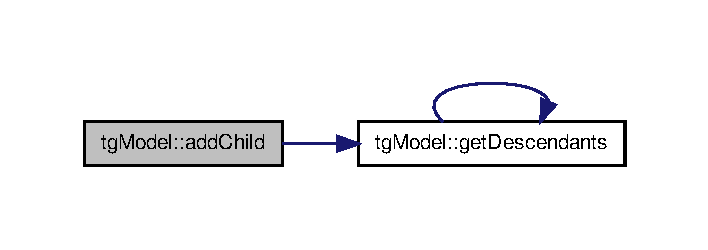
\includegraphics[width=340pt]{classtg_model_a292c17848b96caee32b2286e44c13f2f_cgraph}
\end{center}
\end{figure}




Here is the caller graph for this function\-:\nopagebreak
\begin{figure}[H]
\begin{center}
\leavevmode
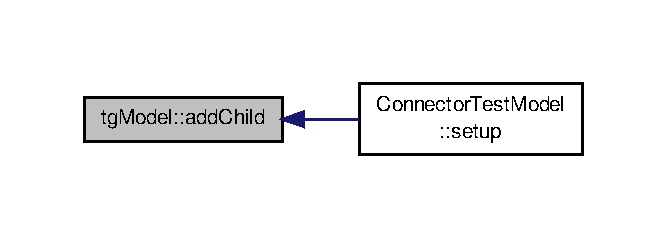
\includegraphics[width=320pt]{classtg_model_a292c17848b96caee32b2286e44c13f2f_icgraph}
\end{center}
\end{figure}


\hypertarget{classtg_subject_a56ecfd33a048c3a7f1a884318d9af548}{\index{Build\-Test\-Model@{Build\-Test\-Model}!attach@{attach}}
\index{attach@{attach}!BuildTestModel@{Build\-Test\-Model}}
\subsubsection[{attach}]{\setlength{\rightskip}{0pt plus 5cm}void {\bf tg\-Subject}$<$ {\bf Build\-Test\-Model}  $>$\-::attach (
\begin{DoxyParamCaption}
\item[{{\bf tg\-Observer}$<$ {\bf Build\-Test\-Model}  $>$ $\ast$}]{p\-Observer}
\end{DoxyParamCaption}
)\hspace{0.3cm}{\ttfamily [inherited]}}}\label{classtg_subject_a56ecfd33a048c3a7f1a884318d9af548}
Attach an observer to the subject of the observer. 
\begin{DoxyParams}[1]{Parameters}
\mbox{\tt in,out}  & {\em p\-Observer} & a pointer to an observer for the subject; do nothing if the pointer is N\-U\-L\-L \\
\hline
\end{DoxyParams}
\hypertarget{classtg_model_ab75836fdfbd9200f165c3b28a19630c0}{\index{Build\-Test\-Model@{Build\-Test\-Model}!find@{find}}
\index{find@{find}!BuildTestModel@{Build\-Test\-Model}}
\subsubsection[{find}]{\setlength{\rightskip}{0pt plus 5cm}template$<$typename T $>$ std\-::vector$<$T$\ast$$>$ tg\-Model\-::find (
\begin{DoxyParamCaption}
\item[{const {\bf tg\-Tag\-Search} \&}]{tag\-Search}
\end{DoxyParamCaption}
)\hspace{0.3cm}{\ttfamily [inline]}, {\ttfamily [inherited]}}}\label{classtg_model_ab75836fdfbd9200f165c3b28a19630c0}
Get a vector of descendants sorted by type and a tagsearch. Useful for pulling out muscle groups, or similar. 
\begin{DoxyParams}[1]{Parameters}
\mbox{\tt in}  & {\em tag\-Search,a} & tag\-Search that contains the desired tags \\
\hline
\end{DoxyParams}
\begin{DoxyReturn}{Returns}
a std\-::vector of pointers to members that match the tag search and typename T 
\end{DoxyReturn}


Definition at line 129 of file tg\-Model.\-h.



Here is the call graph for this function\-:\nopagebreak
\begin{figure}[H]
\begin{center}
\leavevmode
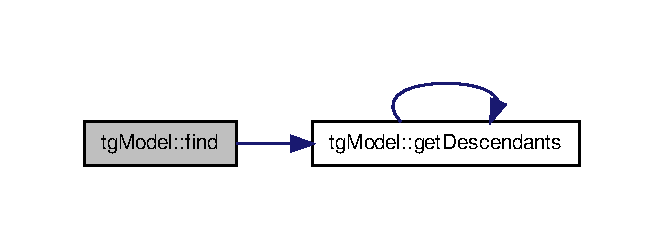
\includegraphics[width=318pt]{classtg_model_ab75836fdfbd9200f165c3b28a19630c0_cgraph}
\end{center}
\end{figure}


\hypertarget{classtg_model_aa40b5fb32f8941e04d537f4e6c6db35c}{\index{Build\-Test\-Model@{Build\-Test\-Model}!find@{find}}
\index{find@{find}!BuildTestModel@{Build\-Test\-Model}}
\subsubsection[{find}]{\setlength{\rightskip}{0pt plus 5cm}template$<$typename T $>$ std\-::vector$<$T$\ast$$>$ tg\-Model\-::find (
\begin{DoxyParamCaption}
\item[{const std\-::string \&}]{tag\-Search}
\end{DoxyParamCaption}
)\hspace{0.3cm}{\ttfamily [inline]}, {\ttfamily [inherited]}}}\label{classtg_model_aa40b5fb32f8941e04d537f4e6c6db35c}
Get a vector of descendants sorted by type and a tagsearch. Useful for pulling out muscle groups, or similar. 
\begin{DoxyParams}[1]{Parameters}
\mbox{\tt in}  & {\em tag\-Search,a} & std\-::string\& that contains the desired tags \\
\hline
\end{DoxyParams}
\begin{DoxyReturn}{Returns}
a std\-::vector of pointers to members that match the tag search and typename T 
\end{DoxyReturn}


Definition at line 142 of file tg\-Model.\-h.



Here is the call graph for this function\-:\nopagebreak
\begin{figure}[H]
\begin{center}
\leavevmode
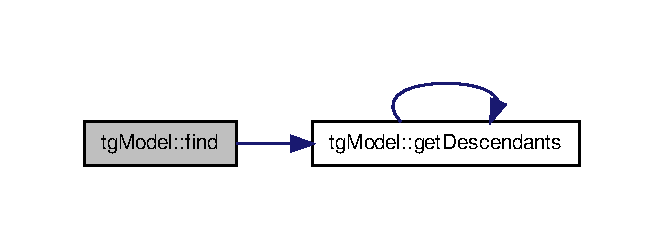
\includegraphics[width=318pt]{classtg_model_aa40b5fb32f8941e04d537f4e6c6db35c_cgraph}
\end{center}
\end{figure}


\hypertarget{classtg_model_a2efa4321fa5c77b4ce23b01f6fd3a1c4}{\index{Build\-Test\-Model@{Build\-Test\-Model}!get\-Descendants@{get\-Descendants}}
\index{get\-Descendants@{get\-Descendants}!BuildTestModel@{Build\-Test\-Model}}
\subsubsection[{get\-Descendants}]{\setlength{\rightskip}{0pt plus 5cm}std\-::vector$<$ {\bf tg\-Model} $\ast$ $>$ tg\-Model\-::get\-Descendants (
\begin{DoxyParamCaption}
{}
\end{DoxyParamCaption}
) const\hspace{0.3cm}{\ttfamily [inherited]}}}\label{classtg_model_a2efa4321fa5c77b4ce23b01f6fd3a1c4}
Return a std\-::vector of const pointers to all sub-\/models. \begin{DoxyRefDesc}{Todo}
\item[\hyperlink{todo__todo000017}{Todo}]examine whether this should be public, and perhaps create a read only version \end{DoxyRefDesc}
\begin{DoxyReturn}{Returns}
a std\-::vector of const pointers all sub-\/models.
\end{DoxyReturn}
\begin{DoxyRefDesc}{Todo}
\item[\hyperlink{todo__todo000014}{Todo}]Unnecessary copying can be avoided by pasing the result collection in the recursive step. \end{DoxyRefDesc}


Definition at line 174 of file tg\-Model.\-cpp.



Here is the call graph for this function\-:\nopagebreak
\begin{figure}[H]
\begin{center}
\leavevmode
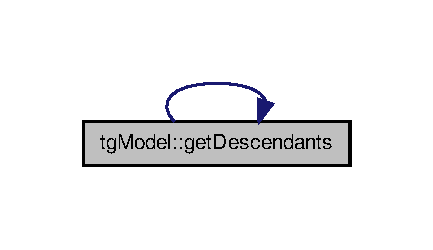
\includegraphics[width=208pt]{classtg_model_a2efa4321fa5c77b4ce23b01f6fd3a1c4_cgraph}
\end{center}
\end{figure}


\hypertarget{classtg_subject_a80799e5d0c8512d3d05a55764790392b}{\index{Build\-Test\-Model@{Build\-Test\-Model}!notify\-Setup@{notify\-Setup}}
\index{notify\-Setup@{notify\-Setup}!BuildTestModel@{Build\-Test\-Model}}
\subsubsection[{notify\-Setup}]{\setlength{\rightskip}{0pt plus 5cm}void {\bf tg\-Subject}$<$ {\bf Build\-Test\-Model}  $>$\-::notify\-Setup (
\begin{DoxyParamCaption}
{}
\end{DoxyParamCaption}
)\hspace{0.3cm}{\ttfamily [inherited]}}}\label{classtg_subject_a80799e5d0c8512d3d05a55764790392b}
Call \hyperlink{classtg_observer_ae7b2de87bd4a6e786bc16f1b801c36a6}{tg\-Observer$<$\-T$>$\-::on\-Setup()} on all observers in the order in which they were attached. \hypertarget{classtg_subject_ad9640aa7fcc1e0b4ce8a913a4ce1ea42}{\index{Build\-Test\-Model@{Build\-Test\-Model}!notify\-Step@{notify\-Step}}
\index{notify\-Step@{notify\-Step}!BuildTestModel@{Build\-Test\-Model}}
\subsubsection[{notify\-Step}]{\setlength{\rightskip}{0pt plus 5cm}void {\bf tg\-Subject}$<$ {\bf Build\-Test\-Model}  $>$\-::notify\-Step (
\begin{DoxyParamCaption}
\item[{double}]{dt}
\end{DoxyParamCaption}
)\hspace{0.3cm}{\ttfamily [inherited]}}}\label{classtg_subject_ad9640aa7fcc1e0b4ce8a913a4ce1ea42}
Call \hyperlink{classtg_observer_a6db5ef1e2792102b8e36dbad5e1a3d7a}{tg\-Observer$<$\-T$>$\-::on\-Step()} on all observers in the order in which they were attached. 
\begin{DoxyParams}[1]{Parameters}
\mbox{\tt in}  & {\em dt} & the number of seconds since the previous call; do nothing if not positive \\
\hline
\end{DoxyParams}


Here is the caller graph for this function\-:
\nopagebreak
\begin{figure}[H]
\begin{center}
\leavevmode
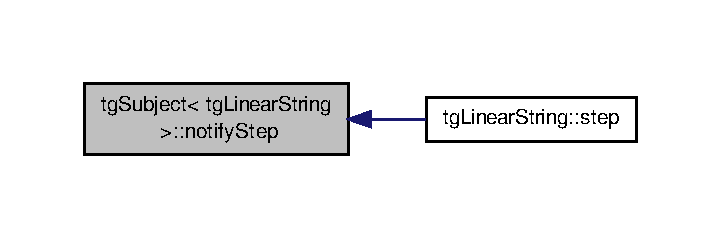
\includegraphics[width=346pt]{classtg_subject_ad9640aa7fcc1e0b4ce8a913a4ce1ea42_icgraph}
\end{center}
\end{figure}


\hypertarget{classtg_subject_adf7a60dbb0faf0de5528f862e7953e63}{\index{Build\-Test\-Model@{Build\-Test\-Model}!notify\-Teardown@{notify\-Teardown}}
\index{notify\-Teardown@{notify\-Teardown}!BuildTestModel@{Build\-Test\-Model}}
\subsubsection[{notify\-Teardown}]{\setlength{\rightskip}{0pt plus 5cm}void {\bf tg\-Subject}$<$ {\bf Build\-Test\-Model}  $>$\-::notify\-Teardown (
\begin{DoxyParamCaption}
{}
\end{DoxyParamCaption}
)\hspace{0.3cm}{\ttfamily [inherited]}}}\label{classtg_subject_adf7a60dbb0faf0de5528f862e7953e63}
Call \hyperlink{classtg_observer_a1663edb3732e5ffb7bbe6bfb4ade88b8}{tg\-Observer$<$\-T$>$\-::on\-Teardown()} on all observers in the order in which they were attached. \hypertarget{class_build_test_model_a8f12c5e787faba7606bbd46531819a4b}{\index{Build\-Test\-Model@{Build\-Test\-Model}!on\-Visit@{on\-Visit}}
\index{on\-Visit@{on\-Visit}!BuildTestModel@{Build\-Test\-Model}}
\subsubsection[{on\-Visit}]{\setlength{\rightskip}{0pt plus 5cm}virtual void Build\-Test\-Model\-::on\-Visit (
\begin{DoxyParamCaption}
\item[{const {\bf tg\-Model\-Visitor} \&}]{r}
\end{DoxyParamCaption}
) const\hspace{0.3cm}{\ttfamily [inline]}, {\ttfamily [virtual]}}}\label{class_build_test_model_a8f12c5e787faba7606bbd46531819a4b}
Call \hyperlink{classtg_model_visitor_a69d056cf31bb4eeef03c243a86f59cc1}{tg\-Model\-Visitor\-::render()} on self and all descendants. 
\begin{DoxyParams}[1]{Parameters}
\mbox{\tt in,out}  & {\em r} & a reference to a \hyperlink{classtg_model_visitor}{tg\-Model\-Visitor} \\
\hline
\end{DoxyParams}


Reimplemented from \hyperlink{classtg_model_aee6457e0fc54d5570b87bfc779f9b1c0}{tg\-Model}.



Definition at line 150 of file Build\-Test\-Model.\-h.

\hypertarget{class_build_test_model_ac41e963bca43e2bc670e18f0801671f7}{\index{Build\-Test\-Model@{Build\-Test\-Model}!setup@{setup}}
\index{setup@{setup}!BuildTestModel@{Build\-Test\-Model}}
\subsubsection[{setup}]{\setlength{\rightskip}{0pt plus 5cm}virtual void Build\-Test\-Model\-::setup (
\begin{DoxyParamCaption}
\item[{{\bf tg\-World} \&}]{world}
\end{DoxyParamCaption}
)\hspace{0.3cm}{\ttfamily [inline]}, {\ttfamily [virtual]}}}\label{class_build_test_model_ac41e963bca43e2bc670e18f0801671f7}
Setup takes a \hyperlink{classtg_world}{tg\-World} and passes it to any children for their own setup functions. All subclasses should call this at the appropriate time (usually end of setup) within their own setup function. 
\begin{DoxyParams}[1]{Parameters}
\mbox{\tt in}  & {\em world} & -\/ the \hyperlink{classtg_world}{tg\-World} the models will exist in. \\
\hline
\end{DoxyParams}


Reimplemented from \hyperlink{classtg_model_a85c68e064972f67c61c47ead392cf6f8}{tg\-Model}.



Definition at line 50 of file Build\-Test\-Model.\-h.



Here is the call graph for this function\-:\nopagebreak
\begin{figure}[H]
\begin{center}
\leavevmode
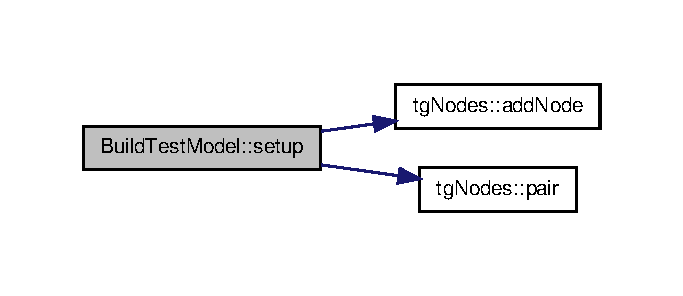
\includegraphics[width=328pt]{class_build_test_model_ac41e963bca43e2bc670e18f0801671f7_cgraph}
\end{center}
\end{figure}


\hypertarget{class_build_test_model_aabd9261840e8466e8648585ccca67397}{\index{Build\-Test\-Model@{Build\-Test\-Model}!step@{step}}
\index{step@{step}!BuildTestModel@{Build\-Test\-Model}}
\subsubsection[{step}]{\setlength{\rightskip}{0pt plus 5cm}virtual void Build\-Test\-Model\-::step (
\begin{DoxyParamCaption}
\item[{double}]{dt}
\end{DoxyParamCaption}
)\hspace{0.3cm}{\ttfamily [inline]}, {\ttfamily [virtual]}}}\label{class_build_test_model_aabd9261840e8466e8648585ccca67397}
Advance the simulation. 
\begin{DoxyParams}[1]{Parameters}
\mbox{\tt in}  & {\em dt} & the number of seconds since the previous call; std\-::invalid\-\_\-argument is thrown if dt is not positive \\
\hline
\end{DoxyParams}

\begin{DoxyExceptions}{Exceptions}
{\em std\-::invalid\-\_\-argument} & if dt is not positive \\
\hline
\end{DoxyExceptions}
\begin{DoxyNote}{Note}
This is not necessarily const for every child. 
\end{DoxyNote}


Reimplemented from \hyperlink{classtg_model_acc6f9ae005f9f51447d7efe5f1815737}{tg\-Model}.



Definition at line 138 of file Build\-Test\-Model.\-h.



Here is the call graph for this function\-:\nopagebreak
\begin{figure}[H]
\begin{center}
\leavevmode
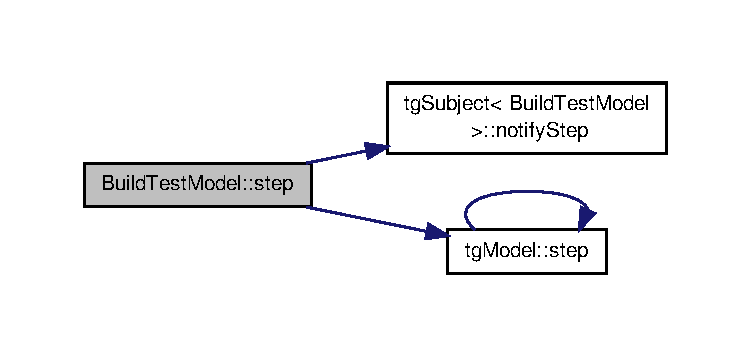
\includegraphics[width=350pt]{class_build_test_model_aabd9261840e8466e8648585ccca67397_cgraph}
\end{center}
\end{figure}


\hypertarget{classtg_model_adb5eec1dcf70a8c039850aea144dcc7e}{\index{Build\-Test\-Model@{Build\-Test\-Model}!teardown@{teardown}}
\index{teardown@{teardown}!BuildTestModel@{Build\-Test\-Model}}
\subsubsection[{teardown}]{\setlength{\rightskip}{0pt plus 5cm}void tg\-Model\-::teardown (
\begin{DoxyParamCaption}
{}
\end{DoxyParamCaption}
)\hspace{0.3cm}{\ttfamily [virtual]}, {\ttfamily [inherited]}}}\label{classtg_model_adb5eec1dcf70a8c039850aea144dcc7e}
Deletes the children (undoes setup) 

Reimplemented in \hyperlink{classtg_base_string_ae4470639491da403b0a29ef0f11ac7b2}{tg\-Base\-String}, \hyperlink{class_contact_test_model_ad9bf515fa080ba02f1ca304aad47aee9}{Contact\-Test\-Model}, \hyperlink{classtg_rod_a7a12ab9a8190c95c28c2dd6749bb1c8c}{tg\-Rod}, \hyperlink{class_prism_model_ac2b643c26c4e27a27714ea07f274654a}{Prism\-Model}, \hyperlink{classtg_r_b_string_a5f4f77b849a87188569a528937f90a97}{tg\-R\-B\-String}, \hyperlink{classtg_linear_string_a1c4be827e518aa1fc944dd14895b3892}{tg\-Linear\-String}, \hyperlink{class_t6_model_ae46a765cf98ef3b17c4540ee4517c343}{T6\-Model}, \hyperlink{class_spiral_spine_a72bb17d2fabd672ae79dcd80c598303a}{Spiral\-Spine}, \hyperlink{class_base_spine_model_learning_aa04ab240035720769a95c403c1f61f73}{Base\-Spine\-Model\-Learning}, \hyperlink{class_j_early_model_a0883e6fcb262de284dcca1bc91b76154}{J\-Early\-Model}, \hyperlink{class_nested_spiral_spine_aea6ab5feee049adfb73835c848366392}{Nested\-Spiral\-Spine}, \hyperlink{class_flemons_spine_model_learning_a489aeb8529c20f9a2473812ea0e78f41}{Flemons\-Spine\-Model\-Learning}, \hyperlink{class_flemons_spine_model_learning_ab2f98f3230f4980bed706d9337a2fae5}{Flemons\-Spine\-Model\-Learning}, \hyperlink{class_tetra_spine_learning_model_a242f0c007fb565c278a26b4efcc299f4}{Tetra\-Spine\-Learning\-Model}, and \hyperlink{class_rib_model_a1f44d22a7213cd3042383c56dcbac61f}{Rib\-Model}.



Definition at line 73 of file tg\-Model.\-cpp.

\hypertarget{classtg_model_af37b0c1a6d4060bfe0bb9b5038a17725}{\index{Build\-Test\-Model@{Build\-Test\-Model}!to\-String@{to\-String}}
\index{to\-String@{to\-String}!BuildTestModel@{Build\-Test\-Model}}
\subsubsection[{to\-String}]{\setlength{\rightskip}{0pt plus 5cm}std\-::string tg\-Model\-::to\-String (
\begin{DoxyParamCaption}
\item[{std\-::string}]{prefix = {\ttfamily \char`\"{}\char`\"{}}}
\end{DoxyParamCaption}
) const\hspace{0.3cm}{\ttfamily [virtual]}, {\ttfamily [inherited]}}}\label{classtg_model_af37b0c1a6d4060bfe0bb9b5038a17725}
Returns the tag names of this model and its children 
\begin{DoxyParams}[1]{Parameters}
\mbox{\tt in}  & {\em prefix} & a string to append to \\
\hline
\end{DoxyParams}
\begin{DoxyReturn}{Returns}
the original string with this model and its children's tags appended 
\end{DoxyReturn}


Definition at line 156 of file tg\-Model.\-cpp.



Here is the caller graph for this function\-:\nopagebreak
\begin{figure}[H]
\begin{center}
\leavevmode
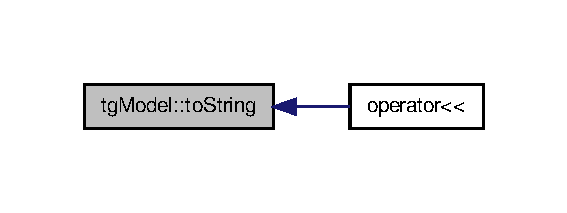
\includegraphics[width=272pt]{classtg_model_af37b0c1a6d4060bfe0bb9b5038a17725_icgraph}
\end{center}
\end{figure}




The documentation for this class was generated from the following file\-:\begin{DoxyCompactItemize}
\item 
dev/tests/Build\-Test\-Model.\-h\end{DoxyCompactItemize}

\hypertarget{struct_r_b_string_test_1_1_config}{\section{R\-B\-String\-Test\-:\-:Config Struct Reference}
\label{struct_r_b_string_test_1_1_config}\index{R\-B\-String\-Test\-::\-Config@{R\-B\-String\-Test\-::\-Config}}
}


Collaboration diagram for R\-B\-String\-Test\-:\-:Config\-:\nopagebreak
\begin{figure}[H]
\begin{center}
\leavevmode
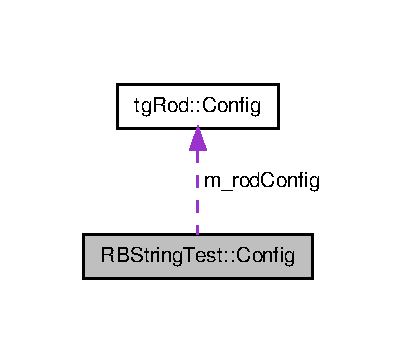
\includegraphics[width=194pt]{struct_r_b_string_test_1_1_config__coll__graph}
\end{center}
\end{figure}
\subsection*{Public Member Functions}
\begin{DoxyCompactItemize}
\item 
\hypertarget{struct_r_b_string_test_1_1_config_a00f03b2c4223e1d803ffe5a1e7af0f86}{{\bfseries Config} (int segments, const \hyperlink{structtg_rod_1_1_config}{tg\-Rod\-::\-Config} \&rod\-Conf, const \hyperlink{structtg_base_string_1_1_config}{tg\-Linear\-String\-::\-Config} \&string\-Conf, double min\-Total\-Length=0.\-1)}\label{struct_r_b_string_test_1_1_config_a00f03b2c4223e1d803ffe5a1e7af0f86}

\end{DoxyCompactItemize}
\subsection*{Public Attributes}
\begin{DoxyCompactItemize}
\item 
\hypertarget{struct_r_b_string_test_1_1_config_a5cfa2fc389ff0767f2814cf5175e9822}{int {\bfseries m\-\_\-segments}}\label{struct_r_b_string_test_1_1_config_a5cfa2fc389ff0767f2814cf5175e9822}

\item 
\hypertarget{struct_r_b_string_test_1_1_config_a58993dfb6faa7ae2786c1b56e8b0b051}{\hyperlink{structtg_rod_1_1_config}{tg\-Rod\-::\-Config} {\bfseries m\-\_\-rod\-Config}}\label{struct_r_b_string_test_1_1_config_a58993dfb6faa7ae2786c1b56e8b0b051}

\item 
\hypertarget{struct_r_b_string_test_1_1_config_aad28f4f3700c30f4edad9a45035e2d63}{\hyperlink{structtg_base_string_1_1_config}{tg\-Linear\-String\-::\-Config} {\bfseries m\-\_\-string\-Config}}\label{struct_r_b_string_test_1_1_config_aad28f4f3700c30f4edad9a45035e2d63}

\item 
\hypertarget{struct_r_b_string_test_1_1_config_ab09fde86fa4b9ea1f5fd3afbccb83dc8}{double {\bfseries m\-\_\-min\-Total\-Length}}\label{struct_r_b_string_test_1_1_config_ab09fde86fa4b9ea1f5fd3afbccb83dc8}

\end{DoxyCompactItemize}


\subsection{Detailed Description}


Definition at line 41 of file R\-B\-String\-Test.\-h.



The documentation for this struct was generated from the following files\-:\begin{DoxyCompactItemize}
\item 
dev/tests/R\-B\-String\-Test.\-h\item 
dev/tests/R\-B\-String\-Test.\-cpp\end{DoxyCompactItemize}

\hypertarget{structtg_box_ground_1_1_config}{\section{tg\-Box\-Ground\-:\-:Config Struct Reference}
\label{structtg_box_ground_1_1_config}\index{tg\-Box\-Ground\-::\-Config@{tg\-Box\-Ground\-::\-Config}}
}
\subsection*{Public Member Functions}
\begin{DoxyCompactItemize}
\item 
\hypertarget{structtg_box_ground_1_1_config_ac6c9f68defbd667bce073757e1756243}{{\bfseries Config} (bt\-Vector3 euler\-Angles=bt\-Vector3(0.\-0, 0.\-0, 0.\-0), bt\-Scalar friction=0.\-5, bt\-Scalar restitution=0.\-0, bt\-Vector3 size=bt\-Vector3(500.\-0, 0.\-5, 500.\-0), bt\-Vector3 origin=bt\-Vector3(0.\-0, 0.\-0, 0.\-0))}\label{structtg_box_ground_1_1_config_ac6c9f68defbd667bce073757e1756243}

\end{DoxyCompactItemize}
\subsection*{Public Attributes}
\begin{DoxyCompactItemize}
\item 
bt\-Vector3 \hyperlink{structtg_box_ground_1_1_config_ada74ac4724fe8f9f7a74fc90d7e93110}{m\-\_\-euler\-Angles}
\item 
bt\-Scalar \hyperlink{structtg_box_ground_1_1_config_ad81773afa88c71825e73ac999a8f3062}{m\-\_\-friction}
\item 
bt\-Scalar \hyperlink{structtg_box_ground_1_1_config_ae8bceb792bc8c1b558e0ef7c12ec8332}{m\-\_\-restitution}
\item 
bt\-Vector3 \hyperlink{structtg_box_ground_1_1_config_a1873e1e4cc14f026e3df1ffb6c0c8156}{m\-\_\-size}
\item 
bt\-Vector3 \hyperlink{structtg_box_ground_1_1_config_a30afd89f94bd4634a45c3dae1cf1628c}{m\-\_\-origin}
\end{DoxyCompactItemize}


\subsection{Detailed Description}


Definition at line 51 of file tg\-Box\-Ground.\-h.



\subsection{Member Data Documentation}
\hypertarget{structtg_box_ground_1_1_config_ada74ac4724fe8f9f7a74fc90d7e93110}{\index{tg\-Box\-Ground\-::\-Config@{tg\-Box\-Ground\-::\-Config}!m\-\_\-euler\-Angles@{m\-\_\-euler\-Angles}}
\index{m\-\_\-euler\-Angles@{m\-\_\-euler\-Angles}!tgBoxGround::Config@{tg\-Box\-Ground\-::\-Config}}
\subsubsection[{m\-\_\-euler\-Angles}]{\setlength{\rightskip}{0pt plus 5cm}bt\-Vector3 tg\-Box\-Ground\-::\-Config\-::m\-\_\-euler\-Angles}}\label{structtg_box_ground_1_1_config_ada74ac4724fe8f9f7a74fc90d7e93110}
Euler angles are specified as yaw pitch and roll 

Definition at line 62 of file tg\-Box\-Ground.\-h.

\hypertarget{structtg_box_ground_1_1_config_ad81773afa88c71825e73ac999a8f3062}{\index{tg\-Box\-Ground\-::\-Config@{tg\-Box\-Ground\-::\-Config}!m\-\_\-friction@{m\-\_\-friction}}
\index{m\-\_\-friction@{m\-\_\-friction}!tgBoxGround::Config@{tg\-Box\-Ground\-::\-Config}}
\subsubsection[{m\-\_\-friction}]{\setlength{\rightskip}{0pt plus 5cm}bt\-Scalar tg\-Box\-Ground\-::\-Config\-::m\-\_\-friction}}\label{structtg_box_ground_1_1_config_ad81773afa88c71825e73ac999a8f3062}
Friction value of the ground, must be between 0 to 1 

Definition at line 67 of file tg\-Box\-Ground.\-h.

\hypertarget{structtg_box_ground_1_1_config_a30afd89f94bd4634a45c3dae1cf1628c}{\index{tg\-Box\-Ground\-::\-Config@{tg\-Box\-Ground\-::\-Config}!m\-\_\-origin@{m\-\_\-origin}}
\index{m\-\_\-origin@{m\-\_\-origin}!tgBoxGround::Config@{tg\-Box\-Ground\-::\-Config}}
\subsubsection[{m\-\_\-origin}]{\setlength{\rightskip}{0pt plus 5cm}bt\-Vector3 tg\-Box\-Ground\-::\-Config\-::m\-\_\-origin}}\label{structtg_box_ground_1_1_config_a30afd89f94bd4634a45c3dae1cf1628c}
Origin position of the ground 

Definition at line 82 of file tg\-Box\-Ground.\-h.

\hypertarget{structtg_box_ground_1_1_config_ae8bceb792bc8c1b558e0ef7c12ec8332}{\index{tg\-Box\-Ground\-::\-Config@{tg\-Box\-Ground\-::\-Config}!m\-\_\-restitution@{m\-\_\-restitution}}
\index{m\-\_\-restitution@{m\-\_\-restitution}!tgBoxGround::Config@{tg\-Box\-Ground\-::\-Config}}
\subsubsection[{m\-\_\-restitution}]{\setlength{\rightskip}{0pt plus 5cm}bt\-Scalar tg\-Box\-Ground\-::\-Config\-::m\-\_\-restitution}}\label{structtg_box_ground_1_1_config_ae8bceb792bc8c1b558e0ef7c12ec8332}
Restitution coefficient of the ground, must be between 0 to 1 

Definition at line 72 of file tg\-Box\-Ground.\-h.

\hypertarget{structtg_box_ground_1_1_config_a1873e1e4cc14f026e3df1ffb6c0c8156}{\index{tg\-Box\-Ground\-::\-Config@{tg\-Box\-Ground\-::\-Config}!m\-\_\-size@{m\-\_\-size}}
\index{m\-\_\-size@{m\-\_\-size}!tgBoxGround::Config@{tg\-Box\-Ground\-::\-Config}}
\subsubsection[{m\-\_\-size}]{\setlength{\rightskip}{0pt plus 5cm}bt\-Vector3 tg\-Box\-Ground\-::\-Config\-::m\-\_\-size}}\label{structtg_box_ground_1_1_config_a1873e1e4cc14f026e3df1ffb6c0c8156}
Size of the ground, must be between non-\/negitive 

Definition at line 77 of file tg\-Box\-Ground.\-h.



The documentation for this struct was generated from the following files\-:\begin{DoxyCompactItemize}
\item 
core/terrain/\hyperlink{tg_box_ground_8h}{tg\-Box\-Ground.\-h}\item 
core/terrain/\hyperlink{tg_box_ground_8cpp}{tg\-Box\-Ground.\-cpp}\end{DoxyCompactItemize}

\hypertarget{struct_base_spine_c_p_g_control_1_1_config}{\section{Base\-Spine\-C\-P\-G\-Control\-:\-:Config Struct Reference}
\label{struct_base_spine_c_p_g_control_1_1_config}\index{Base\-Spine\-C\-P\-G\-Control\-::\-Config@{Base\-Spine\-C\-P\-G\-Control\-::\-Config}}
}
\subsection*{Public Member Functions}
\begin{DoxyCompactItemize}
\item 
\hyperlink{struct_base_spine_c_p_g_control_1_1_config_ad43e25ce15e0e29aa2a4749d07887f14}{Config} (int ss, int tm, int om, int param, int segnum=6, double ct=0.\-1, double la=0, double ha=30, double lp=-\/1 $\ast$M\-\_\-\-P\-I, double hp=M\-\_\-\-P\-I, double kt=0.\-0, double kp=1000.\-0, double kv=100.\-0, bool def=true, double cl=10.\-0)
\end{DoxyCompactItemize}
\subsection*{Public Attributes}
\begin{DoxyCompactItemize}
\item 
\hypertarget{struct_base_spine_c_p_g_control_1_1_config_a4c3a20e52a45b316d6d5412e967ce543}{const int {\bfseries segment\-Span}}\label{struct_base_spine_c_p_g_control_1_1_config_a4c3a20e52a45b316d6d5412e967ce543}

\item 
\hypertarget{struct_base_spine_c_p_g_control_1_1_config_a76e7bc187975749e417552cc65cdcc43}{const int {\bfseries their\-Muscles}}\label{struct_base_spine_c_p_g_control_1_1_config_a76e7bc187975749e417552cc65cdcc43}

\item 
\hypertarget{struct_base_spine_c_p_g_control_1_1_config_a3aeba1da547347b7d322d452c264c97e}{const int {\bfseries our\-Muscles}}\label{struct_base_spine_c_p_g_control_1_1_config_a3aeba1da547347b7d322d452c264c97e}

\item 
\hypertarget{struct_base_spine_c_p_g_control_1_1_config_a81fe14148f1b5fc421004107ecae19ff}{const int {\bfseries params}}\label{struct_base_spine_c_p_g_control_1_1_config_a81fe14148f1b5fc421004107ecae19ff}

\item 
\hypertarget{struct_base_spine_c_p_g_control_1_1_config_a21d430fff6c138e5f16b73fec5797128}{const int {\bfseries segment\-Number}}\label{struct_base_spine_c_p_g_control_1_1_config_a21d430fff6c138e5f16b73fec5797128}

\item 
\hypertarget{struct_base_spine_c_p_g_control_1_1_config_af72c5957b24b82dde192923c88267631}{const double {\bfseries control\-Time}}\label{struct_base_spine_c_p_g_control_1_1_config_af72c5957b24b82dde192923c88267631}

\item 
\hypertarget{struct_base_spine_c_p_g_control_1_1_config_a134e179f186f0b3f03561f73e739a484}{const double {\bfseries low\-Amp}}\label{struct_base_spine_c_p_g_control_1_1_config_a134e179f186f0b3f03561f73e739a484}

\item 
\hypertarget{struct_base_spine_c_p_g_control_1_1_config_a82205fff055235582ab11f5c759ea5e8}{const double {\bfseries high\-Amp}}\label{struct_base_spine_c_p_g_control_1_1_config_a82205fff055235582ab11f5c759ea5e8}

\item 
\hypertarget{struct_base_spine_c_p_g_control_1_1_config_a334aedea7ddcc9e4c5156c81802df39f}{const double {\bfseries low\-Phase}}\label{struct_base_spine_c_p_g_control_1_1_config_a334aedea7ddcc9e4c5156c81802df39f}

\item 
\hypertarget{struct_base_spine_c_p_g_control_1_1_config_a3752344e31e424c346a9285f2d6f9f07}{const double {\bfseries high\-Phase}}\label{struct_base_spine_c_p_g_control_1_1_config_a3752344e31e424c346a9285f2d6f9f07}

\item 
\hypertarget{struct_base_spine_c_p_g_control_1_1_config_ac9d66433de98ee0d8fd05c0d96deb7ef}{const double {\bfseries tension}}\label{struct_base_spine_c_p_g_control_1_1_config_ac9d66433de98ee0d8fd05c0d96deb7ef}

\item 
\hypertarget{struct_base_spine_c_p_g_control_1_1_config_a5f11e2969a872b2771b3961af121f470}{const double {\bfseries k\-Position}}\label{struct_base_spine_c_p_g_control_1_1_config_a5f11e2969a872b2771b3961af121f470}

\item 
\hypertarget{struct_base_spine_c_p_g_control_1_1_config_a5f5968c82f22e82eb9e42de69f703cfb}{const double {\bfseries k\-Velocity}}\label{struct_base_spine_c_p_g_control_1_1_config_a5f5968c82f22e82eb9e42de69f703cfb}

\item 
\hypertarget{struct_base_spine_c_p_g_control_1_1_config_a1398892b6a2fec050598fea12d8bb9cc}{const bool {\bfseries use\-Default}}\label{struct_base_spine_c_p_g_control_1_1_config_a1398892b6a2fec050598fea12d8bb9cc}

\item 
\hypertarget{struct_base_spine_c_p_g_control_1_1_config_a391de1e5ad18fcffe2c41833e2454502}{const double {\bfseries control\-Length}}\label{struct_base_spine_c_p_g_control_1_1_config_a391de1e5ad18fcffe2c41833e2454502}

\end{DoxyCompactItemize}


\subsection{Detailed Description}


Definition at line 47 of file Base\-Spine\-C\-P\-G\-Control.\-h.



\subsection{Constructor \& Destructor Documentation}
\hypertarget{struct_base_spine_c_p_g_control_1_1_config_ad43e25ce15e0e29aa2a4749d07887f14}{\index{Base\-Spine\-C\-P\-G\-Control\-::\-Config@{Base\-Spine\-C\-P\-G\-Control\-::\-Config}!Config@{Config}}
\index{Config@{Config}!BaseSpineCPGControl::Config@{Base\-Spine\-C\-P\-G\-Control\-::\-Config}}
\subsubsection[{Config}]{\setlength{\rightskip}{0pt plus 5cm}Base\-Spine\-C\-P\-G\-Control\-::\-Config\-::\-Config (
\begin{DoxyParamCaption}
\item[{int}]{ss, }
\item[{int}]{tm, }
\item[{int}]{om, }
\item[{int}]{param, }
\item[{int}]{segnum = {\ttfamily 6}, }
\item[{double}]{ct = {\ttfamily 0.1}, }
\item[{double}]{la = {\ttfamily 0}, }
\item[{double}]{ha = {\ttfamily 30}, }
\item[{double}]{lp = {\ttfamily -\/1~$\ast$~M\-\_\-PI}, }
\item[{double}]{hp = {\ttfamily M\-\_\-PI}, }
\item[{double}]{kt = {\ttfamily 0.0}, }
\item[{double}]{kp = {\ttfamily 1000.0}, }
\item[{double}]{kv = {\ttfamily 100.0}, }
\item[{bool}]{def = {\ttfamily true}, }
\item[{double}]{cl = {\ttfamily 10.0}}
\end{DoxyParamCaption}
)}}\label{struct_base_spine_c_p_g_control_1_1_config_ad43e25ce15e0e29aa2a4749d07887f14}
The only constructor. 

Definition at line 38 of file Base\-Spine\-C\-P\-G\-Control.\-cpp.



The documentation for this struct was generated from the following files\-:\begin{DoxyCompactItemize}
\item 
dev/btietz/Base\-Spine\-C\-P\-G\-Control.\-h\item 
dev/btietz/Base\-Spine\-C\-P\-G\-Control.\-cpp\end{DoxyCompactItemize}

\hypertarget{structtg_world_1_1_config}{\section{tg\-World\-:\-:Config Struct Reference}
\label{structtg_world_1_1_config}\index{tg\-World\-::\-Config@{tg\-World\-::\-Config}}
}


{\ttfamily \#include $<$tg\-World.\-h$>$}

\subsection*{Public Attributes}
\begin{DoxyCompactItemize}
\item 
double \hyperlink{structtg_world_1_1_config_a637c1cb122842263847ccf5e84feb854}{gravity}
\end{DoxyCompactItemize}


\subsection{Detailed Description}
World configuration information used by \hyperlink{classtg_world}{tg\-World} constructors. This is Plain Old Data. 

Definition at line 45 of file tg\-World.\-h.



\subsection{Member Data Documentation}
\hypertarget{structtg_world_1_1_config_a637c1cb122842263847ccf5e84feb854}{\index{tg\-World\-::\-Config@{tg\-World\-::\-Config}!gravity@{gravity}}
\index{gravity@{gravity}!tgWorld::Config@{tg\-World\-::\-Config}}
\subsubsection[{gravity}]{\setlength{\rightskip}{0pt plus 5cm}double tg\-World\-::\-Config\-::gravity}}\label{structtg_world_1_1_config_a637c1cb122842263847ccf5e84feb854}
Gravitational acceleration. The units are application depenent. Whether negative values are accepted is application dependent. 

Definition at line 52 of file tg\-World.\-h.



The documentation for this struct was generated from the following file\-:\begin{DoxyCompactItemize}
\item 
core/\hyperlink{tg_world_8h}{tg\-World.\-h}\end{DoxyCompactItemize}

\hypertarget{structtg_base_string_1_1_config}{\section{tg\-Base\-String\-:\-:Config Struct Reference}
\label{structtg_base_string_1_1_config}\index{tg\-Base\-String\-::\-Config@{tg\-Base\-String\-::\-Config}}
}
\subsection*{Public Member Functions}
\begin{DoxyCompactItemize}
\item 
\hyperlink{structtg_base_string_1_1_config_ac40c60ffadf6ea368013580a4cc907bc}{Config} (double s=1000.\-0, double d=10.\-0, bool h=false, double rot=0, double mf=1000.\-0, double t\-Vel=100.\-0, double mx\-Acc=10000.\-0, double mn\-A\-L=0.\-1, double mn\-R\-L=0.\-1)
\item 
void \hyperlink{structtg_base_string_1_1_config_ac5b9fa58a4b3bc751a5e09098e7008ff}{scale} (double sf)
\end{DoxyCompactItemize}
\subsection*{Public Attributes}
\begin{DoxyCompactItemize}
\item 
double \hyperlink{structtg_base_string_1_1_config_a7f0c0e1ddae4ca1594d50bcc9559250e}{stiffness}
\item 
double \hyperlink{structtg_base_string_1_1_config_af4b6fda56bf8480c727b633fad4d27eb}{damping}
\item 
bool \hyperlink{structtg_base_string_1_1_config_ad66c89fe30ffaa19f1ac15de7d5b269b}{hist}
\item 
double \hyperlink{structtg_base_string_1_1_config_adcbba0b56f674d0c38b1fc98e99e3d64}{rotation}
\item 
double \hyperlink{structtg_base_string_1_1_config_a0db6cb3d545d501cd40f2d24545e91e8}{max\-Tens}
\item 
double \hyperlink{structtg_base_string_1_1_config_aec33f58f8ed31fcc41efef395eeca779}{target\-Velocity}
\item 
double \hyperlink{structtg_base_string_1_1_config_aefa59fa6c9a4ea484249ab757632f6cc}{max\-Acc}
\item 
double \hyperlink{structtg_base_string_1_1_config_afda46419afa830031e2a9935d73a75dc}{min\-Actual\-Length}
\item 
double \hyperlink{structtg_base_string_1_1_config_a487963813055e418a148e65d2a3a0d9e}{min\-Rest\-Length}
\end{DoxyCompactItemize}


\subsection{Detailed Description}


Definition at line 46 of file tg\-Base\-String.\-h.



\subsection{Constructor \& Destructor Documentation}
\hypertarget{structtg_base_string_1_1_config_ac40c60ffadf6ea368013580a4cc907bc}{\index{tg\-Base\-String\-::\-Config@{tg\-Base\-String\-::\-Config}!Config@{Config}}
\index{Config@{Config}!tgBaseString::Config@{tg\-Base\-String\-::\-Config}}
\subsubsection[{Config}]{\setlength{\rightskip}{0pt plus 5cm}tg\-Base\-String\-::\-Config\-::\-Config (
\begin{DoxyParamCaption}
\item[{double}]{s = {\ttfamily 1000.0}, }
\item[{double}]{d = {\ttfamily 10.0}, }
\item[{bool}]{h = {\ttfamily false}, }
\item[{double}]{rot = {\ttfamily 0}, }
\item[{double}]{mf = {\ttfamily 1000.0}, }
\item[{double}]{t\-Vel = {\ttfamily 100.0}, }
\item[{double}]{mx\-Acc = {\ttfamily 10000.0}, }
\item[{double}]{mn\-A\-L = {\ttfamily 0.1}, }
\item[{double}]{mn\-R\-L = {\ttfamily 0.1}}
\end{DoxyParamCaption}
)}}\label{structtg_base_string_1_1_config_ac40c60ffadf6ea368013580a4cc907bc}
The only constructor. Parameters set the defaults for string material properties, construction properties and the motor model. Individual parameters are discussed below. \begin{DoxyRefDesc}{Todo}
\item[\hyperlink{todo__todo000007}{Todo}]is this the right place for this, or the constructor of this class? \end{DoxyRefDesc}


Definition at line 36 of file tg\-Base\-String.\-cpp.



\subsection{Member Function Documentation}
\hypertarget{structtg_base_string_1_1_config_ac5b9fa58a4b3bc751a5e09098e7008ff}{\index{tg\-Base\-String\-::\-Config@{tg\-Base\-String\-::\-Config}!scale@{scale}}
\index{scale@{scale}!tgBaseString::Config@{tg\-Base\-String\-::\-Config}}
\subsubsection[{scale}]{\setlength{\rightskip}{0pt plus 5cm}void tg\-Base\-String\-::\-Config\-::scale (
\begin{DoxyParamCaption}
\item[{double}]{sf}
\end{DoxyParamCaption}
)}}\label{structtg_base_string_1_1_config_ac5b9fa58a4b3bc751a5e09098e7008ff}
Scale parameters that depend on the length of the simulation. Centemeter scale has been used throughout many of the demos, so those assumptions are baked into the default parameters. 

Definition at line 82 of file tg\-Base\-String.\-cpp.



\subsection{Member Data Documentation}
\hypertarget{structtg_base_string_1_1_config_af4b6fda56bf8480c727b633fad4d27eb}{\index{tg\-Base\-String\-::\-Config@{tg\-Base\-String\-::\-Config}!damping@{damping}}
\index{damping@{damping}!tgBaseString::Config@{tg\-Base\-String\-::\-Config}}
\subsubsection[{damping}]{\setlength{\rightskip}{0pt plus 5cm}double tg\-Base\-String\-::\-Config\-::damping}}\label{structtg_base_string_1_1_config_af4b6fda56bf8480c727b633fad4d27eb}
Specifies the damping (b) term in the linear force equation. Units are mass / seconds Must be non-\/negative. Similar to stiffness in usage 

Definition at line 85 of file tg\-Base\-String.\-h.

\hypertarget{structtg_base_string_1_1_config_ad66c89fe30ffaa19f1ac15de7d5b269b}{\index{tg\-Base\-String\-::\-Config@{tg\-Base\-String\-::\-Config}!hist@{hist}}
\index{hist@{hist}!tgBaseString::Config@{tg\-Base\-String\-::\-Config}}
\subsubsection[{hist}]{\setlength{\rightskip}{0pt plus 5cm}bool tg\-Base\-String\-::\-Config\-::hist}}\label{structtg_base_string_1_1_config_ad66c89fe30ffaa19f1ac15de7d5b269b}
Specifies whether data such as length and tension will be stored in deque objects. Useful for computing the energy of a trial. 

Definition at line 92 of file tg\-Base\-String.\-h.

\hypertarget{structtg_base_string_1_1_config_aefa59fa6c9a4ea484249ab757632f6cc}{\index{tg\-Base\-String\-::\-Config@{tg\-Base\-String\-::\-Config}!max\-Acc@{max\-Acc}}
\index{max\-Acc@{max\-Acc}!tgBaseString::Config@{tg\-Base\-String\-::\-Config}}
\subsubsection[{max\-Acc}]{\setlength{\rightskip}{0pt plus 5cm}double tg\-Base\-String\-::\-Config\-::max\-Acc}}\label{structtg_base_string_1_1_config_aefa59fa6c9a4ea484249ab757632f6cc}
Maximum acceleration of the motor. This has the largest effect of the limits at small timesteps. Units are length/s$^\wedge$2 Must be nonnegative 

Definition at line 132 of file tg\-Base\-String.\-h.

\hypertarget{structtg_base_string_1_1_config_a0db6cb3d545d501cd40f2d24545e91e8}{\index{tg\-Base\-String\-::\-Config@{tg\-Base\-String\-::\-Config}!max\-Tens@{max\-Tens}}
\index{max\-Tens@{max\-Tens}!tgBaseString::Config@{tg\-Base\-String\-::\-Config}}
\subsubsection[{max\-Tens}]{\setlength{\rightskip}{0pt plus 5cm}double tg\-Base\-String\-::\-Config\-::max\-Tens}}\label{structtg_base_string_1_1_config_a0db6cb3d545d501cd40f2d24545e91e8}
The parameters that affect how the string can be controlled mostly kinematic as of 4/30/14 \begin{DoxyRefDesc}{Todo}
\item[\hyperlink{todo__todo000009}{Todo}]give the motor interia, and specify more things by torque \end{DoxyRefDesc}
Maximum tension that the motor can exert. String will not shorten if this threshold is exceeded, but the tension can still be increased by other members. Units are force (length $\ast$ mass / seconds$^\wedge$2) Must be nonnegative. 

Definition at line 117 of file tg\-Base\-String.\-h.

\hypertarget{structtg_base_string_1_1_config_afda46419afa830031e2a9935d73a75dc}{\index{tg\-Base\-String\-::\-Config@{tg\-Base\-String\-::\-Config}!min\-Actual\-Length@{min\-Actual\-Length}}
\index{min\-Actual\-Length@{min\-Actual\-Length}!tgBaseString::Config@{tg\-Base\-String\-::\-Config}}
\subsubsection[{min\-Actual\-Length}]{\setlength{\rightskip}{0pt plus 5cm}double tg\-Base\-String\-::\-Config\-::min\-Actual\-Length}}\label{structtg_base_string_1_1_config_afda46419afa830031e2a9935d73a75dc}
Actual length below which motor ceases to shorten. Units are length Must be nonnegative 

Definition at line 139 of file tg\-Base\-String.\-h.

\hypertarget{structtg_base_string_1_1_config_a487963813055e418a148e65d2a3a0d9e}{\index{tg\-Base\-String\-::\-Config@{tg\-Base\-String\-::\-Config}!min\-Rest\-Length@{min\-Rest\-Length}}
\index{min\-Rest\-Length@{min\-Rest\-Length}!tgBaseString::Config@{tg\-Base\-String\-::\-Config}}
\subsubsection[{min\-Rest\-Length}]{\setlength{\rightskip}{0pt plus 5cm}double tg\-Base\-String\-::\-Config\-::min\-Rest\-Length}}\label{structtg_base_string_1_1_config_a487963813055e418a148e65d2a3a0d9e}
Rest length below which motor ceases to shorten Units are length Must be nonnegative 

Definition at line 146 of file tg\-Base\-String.\-h.

\hypertarget{structtg_base_string_1_1_config_adcbba0b56f674d0c38b1fc98e99e3d64}{\index{tg\-Base\-String\-::\-Config@{tg\-Base\-String\-::\-Config}!rotation@{rotation}}
\index{rotation@{rotation}!tgBaseString::Config@{tg\-Base\-String\-::\-Config}}
\subsubsection[{rotation}]{\setlength{\rightskip}{0pt plus 5cm}double tg\-Base\-String\-::\-Config\-::rotation}}\label{structtg_base_string_1_1_config_adcbba0b56f674d0c38b1fc98e99e3d64}
Specifies the rotation around the face of the object its attached to. Any value will work, but +/-\/ P\-I is the most meaningful. Units are radians. \begin{DoxyRefDesc}{Todo}
\item[\hyperlink{todo__todo000008}{Todo}]Is this meaningful for non-\/rod shapes? \end{DoxyRefDesc}


Definition at line 101 of file tg\-Base\-String.\-h.

\hypertarget{structtg_base_string_1_1_config_a7f0c0e1ddae4ca1594d50bcc9559250e}{\index{tg\-Base\-String\-::\-Config@{tg\-Base\-String\-::\-Config}!stiffness@{stiffness}}
\index{stiffness@{stiffness}!tgBaseString::Config@{tg\-Base\-String\-::\-Config}}
\subsubsection[{stiffness}]{\setlength{\rightskip}{0pt plus 5cm}double tg\-Base\-String\-::\-Config\-::stiffness}}\label{structtg_base_string_1_1_config_a7f0c0e1ddae4ca1594d50bcc9559250e}
Linear Hookean stiffness of the string (k). Must be non-\/negative. Upper limit depends on the timestep -\/ stiffer springs will require a lower timestep. Used in \hyperlink{class_muscle2_p}{Muscle2\-P}, tension\-Min\-Length\-Controller, move\-Motors (to enforce max force constraints) Units are mass / seconds$^\wedge$2 

Definition at line 79 of file tg\-Base\-String.\-h.

\hypertarget{structtg_base_string_1_1_config_aec33f58f8ed31fcc41efef395eeca779}{\index{tg\-Base\-String\-::\-Config@{tg\-Base\-String\-::\-Config}!target\-Velocity@{target\-Velocity}}
\index{target\-Velocity@{target\-Velocity}!tgBaseString::Config@{tg\-Base\-String\-::\-Config}}
\subsubsection[{target\-Velocity}]{\setlength{\rightskip}{0pt plus 5cm}double tg\-Base\-String\-::\-Config\-::target\-Velocity}}\label{structtg_base_string_1_1_config_aec33f58f8ed31fcc41efef395eeca779}
Maximum velocity of the motor, usage in move\-Motors Units are length/seconds Must be nonnegative. 

Definition at line 124 of file tg\-Base\-String.\-h.



The documentation for this struct was generated from the following files\-:\begin{DoxyCompactItemize}
\item 
core/\hyperlink{tg_base_string_8h}{tg\-Base\-String.\-h}\item 
core/\hyperlink{tg_base_string_8cpp}{tg\-Base\-String.\-cpp}\end{DoxyCompactItemize}

\hypertarget{structtg_rod_1_1_config}{\section{tg\-Rod\-:\-:Config Struct Reference}
\label{structtg_rod_1_1_config}\index{tg\-Rod\-::\-Config@{tg\-Rod\-::\-Config}}
}


{\ttfamily \#include $<$tg\-Rod.\-h$>$}

\subsection*{Public Member Functions}
\begin{DoxyCompactItemize}
\item 
\hyperlink{structtg_rod_1_1_config_ae4f5148db61532a98c75d34dd97a186f}{Config} (double r=0.\-5, double d=1.\-0, double f=0.\-5, double rf=0.\-0, double res=0.\-0)
\end{DoxyCompactItemize}
\subsection*{Public Attributes}
\begin{DoxyCompactItemize}
\item 
const double \hyperlink{structtg_rod_1_1_config_a20c2370d27608ee1d7e8521095f6b0df}{radius}
\item 
const double \hyperlink{structtg_rod_1_1_config_ad4949cc9e0d084a5d0907ee6b89616c7}{density}
\item 
const double \hyperlink{structtg_rod_1_1_config_a7c85c2b9b8f2d30fea1a8c5e498b2fd6}{friction}
\item 
const double \hyperlink{structtg_rod_1_1_config_a99421c0930dce83ed7721fe899611e7c}{roll\-Friction}
\item 
const double \hyperlink{structtg_rod_1_1_config_aa16247d472088ec2476f409da5f92f87}{restitution}
\end{DoxyCompactItemize}


\subsection{Detailed Description}
Holds two public member variables, density and radius, describing a rod configuration. A constructor allows them to be set together and to default. 

Definition at line 51 of file tg\-Rod.\-h.



\subsection{Constructor \& Destructor Documentation}
\hypertarget{structtg_rod_1_1_config_ae4f5148db61532a98c75d34dd97a186f}{\index{tg\-Rod\-::\-Config@{tg\-Rod\-::\-Config}!Config@{Config}}
\index{Config@{Config}!tgRod::Config@{tg\-Rod\-::\-Config}}
\subsubsection[{Config}]{\setlength{\rightskip}{0pt plus 5cm}tg\-Rod\-::\-Config\-::\-Config (
\begin{DoxyParamCaption}
\item[{double}]{r = {\ttfamily 0.5}, }
\item[{double}]{d = {\ttfamily 1.0}, }
\item[{double}]{f = {\ttfamily 0.5}, }
\item[{double}]{rf = {\ttfamily 0.0}, }
\item[{double}]{res = {\ttfamily 0.0}}
\end{DoxyParamCaption}
)}}\label{structtg_rod_1_1_config_ae4f5148db61532a98c75d34dd97a186f}
Initialize with radius and density, which may default. 
\begin{DoxyParams}[1]{Parameters}
\mbox{\tt in}  & {\em radius} & the rod's radius; must be non-\/negative \\
\hline
\mbox{\tt in}  & {\em density} & the rod's density; must be non-\/negative \\
\hline
\end{DoxyParams}


Definition at line 35 of file tg\-Rod.\-cpp.



\subsection{Member Data Documentation}
\hypertarget{structtg_rod_1_1_config_ad4949cc9e0d084a5d0907ee6b89616c7}{\index{tg\-Rod\-::\-Config@{tg\-Rod\-::\-Config}!density@{density}}
\index{density@{density}!tgRod::Config@{tg\-Rod\-::\-Config}}
\subsubsection[{density}]{\setlength{\rightskip}{0pt plus 5cm}const double tg\-Rod\-::\-Config\-::density}}\label{structtg_rod_1_1_config_ad4949cc9e0d084a5d0907ee6b89616c7}
The rod's density; must be nonnegative. 

Definition at line 68 of file tg\-Rod.\-h.

\hypertarget{structtg_rod_1_1_config_a7c85c2b9b8f2d30fea1a8c5e498b2fd6}{\index{tg\-Rod\-::\-Config@{tg\-Rod\-::\-Config}!friction@{friction}}
\index{friction@{friction}!tgRod::Config@{tg\-Rod\-::\-Config}}
\subsubsection[{friction}]{\setlength{\rightskip}{0pt plus 5cm}const double tg\-Rod\-::\-Config\-::friction}}\label{structtg_rod_1_1_config_a7c85c2b9b8f2d30fea1a8c5e498b2fd6}
The rod's friction; must be between 0 and 1 (inclusive). 

Definition at line 72 of file tg\-Rod.\-h.

\hypertarget{structtg_rod_1_1_config_a20c2370d27608ee1d7e8521095f6b0df}{\index{tg\-Rod\-::\-Config@{tg\-Rod\-::\-Config}!radius@{radius}}
\index{radius@{radius}!tgRod::Config@{tg\-Rod\-::\-Config}}
\subsubsection[{radius}]{\setlength{\rightskip}{0pt plus 5cm}const double tg\-Rod\-::\-Config\-::radius}}\label{structtg_rod_1_1_config_a20c2370d27608ee1d7e8521095f6b0df}
The rod's radius; must be nonnegative. 

Definition at line 65 of file tg\-Rod.\-h.

\hypertarget{structtg_rod_1_1_config_aa16247d472088ec2476f409da5f92f87}{\index{tg\-Rod\-::\-Config@{tg\-Rod\-::\-Config}!restitution@{restitution}}
\index{restitution@{restitution}!tgRod::Config@{tg\-Rod\-::\-Config}}
\subsubsection[{restitution}]{\setlength{\rightskip}{0pt plus 5cm}const double tg\-Rod\-::\-Config\-::restitution}}\label{structtg_rod_1_1_config_aa16247d472088ec2476f409da5f92f87}
The rod's coefficient of restitution; must be between 0 and 1 (inclusive). 

Definition at line 80 of file tg\-Rod.\-h.

\hypertarget{structtg_rod_1_1_config_a99421c0930dce83ed7721fe899611e7c}{\index{tg\-Rod\-::\-Config@{tg\-Rod\-::\-Config}!roll\-Friction@{roll\-Friction}}
\index{roll\-Friction@{roll\-Friction}!tgRod::Config@{tg\-Rod\-::\-Config}}
\subsubsection[{roll\-Friction}]{\setlength{\rightskip}{0pt plus 5cm}const double tg\-Rod\-::\-Config\-::roll\-Friction}}\label{structtg_rod_1_1_config_a99421c0930dce83ed7721fe899611e7c}
The rod's rolling friction; must be between 0 and 1 (inclusive). 

Definition at line 76 of file tg\-Rod.\-h.



The documentation for this struct was generated from the following files\-:\begin{DoxyCompactItemize}
\item 
core/\hyperlink{tg_rod_8h}{tg\-Rod.\-h}\item 
core/\hyperlink{tg_rod_8cpp}{tg\-Rod.\-cpp}\end{DoxyCompactItemize}

\hypertarget{structtg_r_b_string_1_1_config}{\section{tg\-R\-B\-String\-:\-:Config Struct Reference}
\label{structtg_r_b_string_1_1_config}\index{tg\-R\-B\-String\-::\-Config@{tg\-R\-B\-String\-::\-Config}}
}


Collaboration diagram for tg\-R\-B\-String\-:\-:Config\-:\nopagebreak
\begin{figure}[H]
\begin{center}
\leavevmode
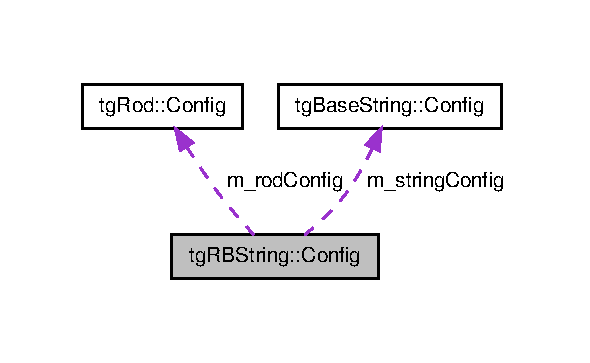
\includegraphics[width=283pt]{structtg_r_b_string_1_1_config__coll__graph}
\end{center}
\end{figure}
\subsection*{Public Member Functions}
\begin{DoxyCompactItemize}
\item 
\hyperlink{structtg_r_b_string_1_1_config_a599e7c66d595cbb500ad71722660d092}{Config} ()
\item 
\hypertarget{structtg_r_b_string_1_1_config_a61dd326c15917436840d364556763fb8}{{\bfseries Config} (std\-::size\-\_\-t segments, const \hyperlink{structtg_rod_1_1_config}{tg\-Rod\-::\-Config} \&rod\-Conf, const \hyperlink{structtg_base_string_1_1_config}{tg\-Base\-String\-::\-Config} \&string\-Conf, double min\-Total\-Length=0.\-1)}\label{structtg_r_b_string_1_1_config_a61dd326c15917436840d364556763fb8}

\end{DoxyCompactItemize}
\subsection*{Public Attributes}
\begin{DoxyCompactItemize}
\item 
\hypertarget{structtg_r_b_string_1_1_config_aa50b82ab844b8b4bfd99080f375d04cd}{std\-::size\-\_\-t {\bfseries m\-\_\-segments}}\label{structtg_r_b_string_1_1_config_aa50b82ab844b8b4bfd99080f375d04cd}

\item 
\hypertarget{structtg_r_b_string_1_1_config_a3c9da412e0a0224b28cf82c546f4c19d}{\hyperlink{structtg_rod_1_1_config}{tg\-Rod\-::\-Config} {\bfseries m\-\_\-rod\-Config}}\label{structtg_r_b_string_1_1_config_a3c9da412e0a0224b28cf82c546f4c19d}

\item 
\hypertarget{structtg_r_b_string_1_1_config_a5e0055cf985d8f26f03df2d4248a28e6}{\hyperlink{structtg_base_string_1_1_config}{tg\-Base\-String\-::\-Config} {\bfseries m\-\_\-string\-Config}}\label{structtg_r_b_string_1_1_config_a5e0055cf985d8f26f03df2d4248a28e6}

\item 
\hypertarget{structtg_r_b_string_1_1_config_a340d82c69228cf86c314cdc675a477fe}{double {\bfseries m\-\_\-min\-Total\-Length}}\label{structtg_r_b_string_1_1_config_a340d82c69228cf86c314cdc675a477fe}

\end{DoxyCompactItemize}


\subsection{Detailed Description}


Definition at line 48 of file tg\-R\-B\-String.\-h.



\subsection{Constructor \& Destructor Documentation}
\hypertarget{structtg_r_b_string_1_1_config_a599e7c66d595cbb500ad71722660d092}{\index{tg\-R\-B\-String\-::\-Config@{tg\-R\-B\-String\-::\-Config}!Config@{Config}}
\index{Config@{Config}!tgRBString::Config@{tg\-R\-B\-String\-::\-Config}}
\subsubsection[{Config}]{\setlength{\rightskip}{0pt plus 5cm}tg\-R\-B\-String\-::\-Config\-::\-Config (
\begin{DoxyParamCaption}
{}
\end{DoxyParamCaption}
)}}\label{structtg_r_b_string_1_1_config_a599e7c66d595cbb500ad71722660d092}
Dummy constructor to make the compiler happy. \begin{DoxyRefDesc}{Todo}
\item[\hyperlink{todo__todo000049}{Todo}]remove this \end{DoxyRefDesc}


Definition at line 41 of file tg\-R\-B\-String.\-cpp.



The documentation for this struct was generated from the following files\-:\begin{DoxyCompactItemize}
\item 
dev/btietz/\hyperlink{tg_r_b_string_8h}{tg\-R\-B\-String.\-h}\item 
dev/btietz/\hyperlink{tg_r_b_string_8cpp}{tg\-R\-B\-String.\-cpp}\end{DoxyCompactItemize}

\hypertarget{classconfiguration}{\section{configuration Class Reference}
\label{classconfiguration}\index{configuration@{configuration}}
}
\subsection*{Public Member Functions}
\begin{DoxyCompactItemize}
\item 
\hyperlink{classconfiguration_ad4446282343ce7dd8a67ffbc15f1d575}{configuration} ()
\item 
\hypertarget{classconfiguration_a2cd390347727161f3663f04f39c13b7f}{bool {\bfseries iskey} (const std\-::string \&s) const }\label{classconfiguration_a2cd390347727161f3663f04f39c13b7f}

\item 
\hypertarget{classconfiguration_adcf1ed053ba6786dafe5e82b04635fd8}{int {\bfseries getintvalue} (const std\-::string \&key)}\label{classconfiguration_adcf1ed053ba6786dafe5e82b04635fd8}

\item 
\hypertarget{classconfiguration_a5aa70bcb9aff4526951b7b9b69ff7bf8}{double {\bfseries get\-Double\-Value} (const std\-::string \&key)}\label{classconfiguration_a5aa70bcb9aff4526951b7b9b69ff7bf8}

\item 
\hypertarget{classconfiguration_ab33d8f8158e394aec793b189a127d925}{std\-::string {\bfseries get\-String\-Value} (const std\-::string \&key)}\label{classconfiguration_ab33d8f8158e394aec793b189a127d925}

\item 
\hypertarget{classconfiguration_a7d48d243abca23456cf3e5c64945f84c}{void {\bfseries read\-File} (const std\-::string filename)}\label{classconfiguration_a7d48d243abca23456cf3e5c64945f84c}

\item 
\hypertarget{classconfiguration_ad1f54f601d26c7d3b6f2319a25b64eba}{void {\bfseries write\-To\-File} (const std\-::string filename)}\label{classconfiguration_ad1f54f601d26c7d3b6f2319a25b64eba}

\end{DoxyCompactItemize}
\subsection*{Public Attributes}
\begin{DoxyCompactItemize}
\item 
\hypertarget{classconfiguration_ac11a1c00053ce7721af0f909744f6085}{std\-::map$<$ std\-::string, \\*
std\-::string $>$ {\bfseries data}}\label{classconfiguration_ac11a1c00053ce7721af0f909744f6085}

\end{DoxyCompactItemize}


\subsection{Detailed Description}


Definition at line 41 of file configuration.\-h.



\subsection{Constructor \& Destructor Documentation}
\hypertarget{classconfiguration_ad4446282343ce7dd8a67ffbc15f1d575}{\index{configuration@{configuration}!configuration@{configuration}}
\index{configuration@{configuration}!configuration@{configuration}}
\subsubsection[{configuration}]{\setlength{\rightskip}{0pt plus 5cm}configuration\-::configuration (
\begin{DoxyParamCaption}
{}
\end{DoxyParamCaption}
)}}\label{classconfiguration_ad4446282343ce7dd8a67ffbc15f1d575}
\begin{DoxyVerb} ---------------------------------------------------------------------------
\end{DoxyVerb}
 The configuration\-::data is a simple map string (key, value) pairs. The file is stored as a simple listing of those pairs, one per line. The key is separated from the value by an equal sign '='. Commentary begins with the first non-\/space character on the line a hash or semi-\/colon ('\#' or ';').

Example\-: \subsection*{This is an example}

source.\-directory = C\-: and Settings Documents\textbackslash{} file.\-types = $\ast$.jpg;$\ast$.gif;$\ast$.png;$\ast$.pix;$\ast$.tif;$\ast$.bmp

Notice that the configuration file format does not permit values to span more than one line, commentary at the end of a line, or \mbox{[}section\mbox{]}s. 

Definition at line 35 of file configuration.\-cpp.



The documentation for this class was generated from the following files\-:\begin{DoxyCompactItemize}
\item 
learning/\-Configuration/\hyperlink{configuration_8h}{configuration.\-h}\item 
learning/\-Configuration/\hyperlink{configuration_8cpp}{configuration.\-cpp}\end{DoxyCompactItemize}

\hypertarget{structtg_build_spec_1_1_connector_agent}{\section{tg\-Build\-Spec\-:\-:Connector\-Agent Struct Reference}
\label{structtg_build_spec_1_1_connector_agent}\index{tg\-Build\-Spec\-::\-Connector\-Agent@{tg\-Build\-Spec\-::\-Connector\-Agent}}
}


Collaboration diagram for tg\-Build\-Spec\-:\-:Connector\-Agent\-:\nopagebreak
\begin{figure}[H]
\begin{center}
\leavevmode
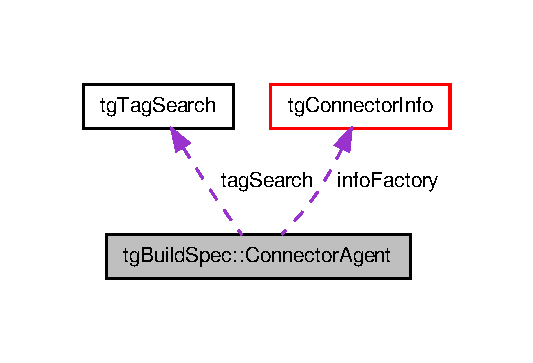
\includegraphics[width=256pt]{structtg_build_spec_1_1_connector_agent__coll__graph}
\end{center}
\end{figure}
\subsection*{Public Member Functions}
\begin{DoxyCompactItemize}
\item 
\hypertarget{structtg_build_spec_1_1_connector_agent_a492d3ea5402b53ad66f2aec8d4ff47a7}{{\bfseries Connector\-Agent} (\hyperlink{classtg_tag_search}{tg\-Tag\-Search} s, \hyperlink{classtg_connector_info}{tg\-Connector\-Info} $\ast$b)}\label{structtg_build_spec_1_1_connector_agent_a492d3ea5402b53ad66f2aec8d4ff47a7}

\item 
\hypertarget{structtg_build_spec_1_1_connector_agent_a29fad7c37cb0ae22981ba74b47ad0bba}{{\bfseries Connector\-Agent} (std\-::string s, \hyperlink{classtg_connector_info}{tg\-Connector\-Info} $\ast$b)}\label{structtg_build_spec_1_1_connector_agent_a29fad7c37cb0ae22981ba74b47ad0bba}

\end{DoxyCompactItemize}
\subsection*{Public Attributes}
\begin{DoxyCompactItemize}
\item 
\hypertarget{structtg_build_spec_1_1_connector_agent_a905f28a41a64416ec46081054b60eda6}{\hyperlink{classtg_tag_search}{tg\-Tag\-Search} {\bfseries tag\-Search}}\label{structtg_build_spec_1_1_connector_agent_a905f28a41a64416ec46081054b60eda6}

\item 
\hypertarget{structtg_build_spec_1_1_connector_agent_af88a5a4bb8092aa8f721e3b4cb289cfd}{\hyperlink{classtg_connector_info}{tg\-Connector\-Info} $\ast$ {\bfseries info\-Factory}}\label{structtg_build_spec_1_1_connector_agent_af88a5a4bb8092aa8f721e3b4cb289cfd}

\end{DoxyCompactItemize}


\subsection{Detailed Description}


Definition at line 73 of file tg\-Build\-Spec.\-h.



The documentation for this struct was generated from the following files\-:\begin{DoxyCompactItemize}
\item 
tgcreator/\hyperlink{tg_build_spec_8h}{tg\-Build\-Spec.\-h}\item 
tgcreator/\hyperlink{tg_build_spec_8cpp}{tg\-Build\-Spec.\-cpp}\end{DoxyCompactItemize}

\hypertarget{class_connector_test_model}{\section{Connector\-Test\-Model Class Reference}
\label{class_connector_test_model}\index{Connector\-Test\-Model@{Connector\-Test\-Model}}
}


Inheritance diagram for Connector\-Test\-Model\-:\nopagebreak
\begin{figure}[H]
\begin{center}
\leavevmode
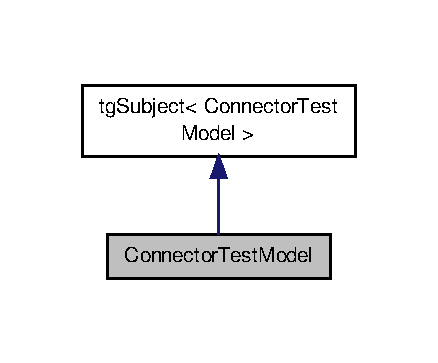
\includegraphics[width=210pt]{class_connector_test_model__inherit__graph}
\end{center}
\end{figure}


Collaboration diagram for Connector\-Test\-Model\-:\nopagebreak
\begin{figure}[H]
\begin{center}
\leavevmode
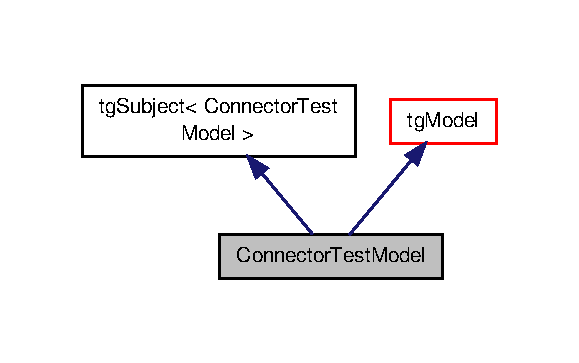
\includegraphics[width=278pt]{class_connector_test_model__coll__graph}
\end{center}
\end{figure}
\subsection*{Public Member Functions}
\begin{DoxyCompactItemize}
\item 
\hypertarget{class_connector_test_model_aea74dce63d88ad55cb01afcc0ef4f62b}{{\bfseries Connector\-Test\-Model} (std\-::string name)}\label{class_connector_test_model_aea74dce63d88ad55cb01afcc0ef4f62b}

\item 
virtual void \hyperlink{class_connector_test_model_a98cee5085d31f5238dd6c5607eef02bf}{setup} (\hyperlink{classtg_world}{tg\-World} \&world)
\item 
virtual void \hyperlink{class_connector_test_model_a30e5b347373f77dc84584569d8ac7b4e}{step} (double dt)
\item 
virtual void \hyperlink{class_connector_test_model_a8d4e146eb48dd23676a5522e9417abdb}{on\-Visit} (const \hyperlink{classtg_model_visitor}{tg\-Model\-Visitor} \&r) const 
\item 
\hypertarget{class_connector_test_model_a2adf3eec12a3bb4f3296830466dbd30f}{void {\bfseries change\-Muscle} (double length)}\label{class_connector_test_model_a2adf3eec12a3bb4f3296830466dbd30f}

\item 
void \hyperlink{classtg_subject_a56ecfd33a048c3a7f1a884318d9af548}{attach} (\hyperlink{classtg_observer}{tg\-Observer}$<$ \hyperlink{class_connector_test_model}{Connector\-Test\-Model} $>$ $\ast$p\-Observer)
\item 
void \hyperlink{classtg_subject_ad9640aa7fcc1e0b4ce8a913a4ce1ea42}{notify\-Step} (double dt)
\item 
void \hyperlink{classtg_subject_a80799e5d0c8512d3d05a55764790392b}{notify\-Setup} ()
\item 
void \hyperlink{classtg_subject_adf7a60dbb0faf0de5528f862e7953e63}{notify\-Teardown} ()
\item 
virtual void \hyperlink{classtg_model_adb5eec1dcf70a8c039850aea144dcc7e}{teardown} ()
\item 
void \hyperlink{classtg_model_a292c17848b96caee32b2286e44c13f2f}{add\-Child} (\hyperlink{classtg_model}{tg\-Model} $\ast$p\-Child)
\item 
virtual std\-::string \hyperlink{classtg_model_af37b0c1a6d4060bfe0bb9b5038a17725}{to\-String} (std\-::string prefix=\char`\"{}\char`\"{}) const 
\item 
{\footnotesize template$<$typename T $>$ }\\std\-::vector$<$ T $\ast$ $>$ \hyperlink{classtg_model_ab75836fdfbd9200f165c3b28a19630c0}{find} (const \hyperlink{classtg_tag_search}{tg\-Tag\-Search} \&tag\-Search)
\item 
{\footnotesize template$<$typename T $>$ }\\std\-::vector$<$ T $\ast$ $>$ \hyperlink{classtg_model_aa40b5fb32f8941e04d537f4e6c6db35c}{find} (const std\-::string \&tag\-Search)
\item 
std\-::vector$<$ \hyperlink{classtg_model}{tg\-Model} $\ast$ $>$ \hyperlink{classtg_model_a2efa4321fa5c77b4ce23b01f6fd3a1c4}{get\-Descendants} () const 
\item 
\hypertarget{classtg_taggable_af0b8f1729653b0b90d2fecbd51163612}{void {\bfseries add\-Tags} (const std\-::string \&space\-\_\-separated\-\_\-tags)}\label{classtg_taggable_af0b8f1729653b0b90d2fecbd51163612}

\item 
\hypertarget{classtg_taggable_af28e3fe1a7e4eb28772dc006d575dd1f}{void {\bfseries add\-Tags} (const \hyperlink{classtg_tags}{tg\-Tags} \&tags)}\label{classtg_taggable_af28e3fe1a7e4eb28772dc006d575dd1f}

\item 
\hypertarget{classtg_taggable_ae31f65869c8887bfeb34a344902c4d5b}{bool {\bfseries has\-Tag} (const std\-::string tag) const }\label{classtg_taggable_ae31f65869c8887bfeb34a344902c4d5b}

\item 
\hypertarget{classtg_taggable_a33b77b1075171b63f673965687b2e844}{bool {\bfseries has\-All\-Tags} (std\-::string tags)}\label{classtg_taggable_a33b77b1075171b63f673965687b2e844}

\item 
\hypertarget{classtg_taggable_af14af28fa98021c4f20a5e8f2ddd5606}{bool {\bfseries has\-Any\-Tags} (const std\-::string tags)}\label{classtg_taggable_af14af28fa98021c4f20a5e8f2ddd5606}

\item 
\hypertarget{classtg_taggable_adff345e116e16420c701a748ff8f995f}{bool {\bfseries has\-No\-Tags} ()}\label{classtg_taggable_adff345e116e16420c701a748ff8f995f}

\item 
\hypertarget{classtg_taggable_acf1d7fa9df8f374f25015c4080902681}{\hyperlink{classtg_tags}{tg\-Tags} \& {\bfseries get\-Tags} ()}\label{classtg_taggable_acf1d7fa9df8f374f25015c4080902681}

\item 
\hypertarget{classtg_taggable_ae70d7d3b45301665bc363b0ed8b9b292}{const \hyperlink{classtg_tags}{tg\-Tags} \& {\bfseries get\-Tags} () const }\label{classtg_taggable_ae70d7d3b45301665bc363b0ed8b9b292}

\item 
\hypertarget{classtg_taggable_a5492888e4e4da4cca6261070b5726adf}{void {\bfseries set\-Tags} (\hyperlink{classtg_tags}{tg\-Tags} tags)}\label{classtg_taggable_a5492888e4e4da4cca6261070b5726adf}

\item 
\hypertarget{classtg_taggable_a346d66b066d2d9eb1eadba01da43749f}{std\-::string {\bfseries get\-Tag\-Str} (std\-::string delim=\char`\"{} \char`\"{}) const }\label{classtg_taggable_a346d66b066d2d9eb1eadba01da43749f}

\end{DoxyCompactItemize}


\subsection{Detailed Description}


Definition at line 38 of file Connector\-Test\-Model.\-h.



\subsection{Member Function Documentation}
\hypertarget{classtg_model_a292c17848b96caee32b2286e44c13f2f}{\index{Connector\-Test\-Model@{Connector\-Test\-Model}!add\-Child@{add\-Child}}
\index{add\-Child@{add\-Child}!ConnectorTestModel@{Connector\-Test\-Model}}
\subsubsection[{add\-Child}]{\setlength{\rightskip}{0pt plus 5cm}void tg\-Model\-::add\-Child (
\begin{DoxyParamCaption}
\item[{{\bf tg\-Model} $\ast$}]{p\-Child}
\end{DoxyParamCaption}
)\hspace{0.3cm}{\ttfamily [inherited]}}}\label{classtg_model_a292c17848b96caee32b2286e44c13f2f}
Add a sub-\/model to this model. The model takes ownership of the child sub-\/model and is responsible for deallocating it. 
\begin{DoxyParams}[1]{Parameters}
\mbox{\tt in,out}  & {\em p\-Child} & a pointer to a sub-\/model \\
\hline
\end{DoxyParams}

\begin{DoxyExceptions}{Exceptions}
{\em std\-::invalid\-\_\-argument} & is p\-Child is N\-U\-L\-L, this object, or already a descendant \\
\hline
\end{DoxyExceptions}
\begin{DoxyRefDesc}{Todo}
\item[\hyperlink{todo__todo000016}{Todo}]Make sure that every child appears no more than once in the tree. \end{DoxyRefDesc}


Definition at line 126 of file tg\-Model.\-cpp.



Here is the call graph for this function\-:\nopagebreak
\begin{figure}[H]
\begin{center}
\leavevmode
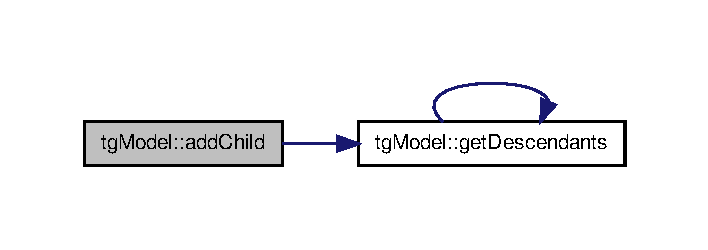
\includegraphics[width=340pt]{classtg_model_a292c17848b96caee32b2286e44c13f2f_cgraph}
\end{center}
\end{figure}




Here is the caller graph for this function\-:\nopagebreak
\begin{figure}[H]
\begin{center}
\leavevmode
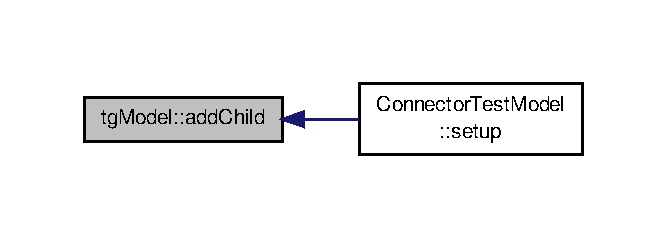
\includegraphics[width=320pt]{classtg_model_a292c17848b96caee32b2286e44c13f2f_icgraph}
\end{center}
\end{figure}


\hypertarget{classtg_subject_a56ecfd33a048c3a7f1a884318d9af548}{\index{Connector\-Test\-Model@{Connector\-Test\-Model}!attach@{attach}}
\index{attach@{attach}!ConnectorTestModel@{Connector\-Test\-Model}}
\subsubsection[{attach}]{\setlength{\rightskip}{0pt plus 5cm}void {\bf tg\-Subject}$<$ {\bf Connector\-Test\-Model}  $>$\-::attach (
\begin{DoxyParamCaption}
\item[{{\bf tg\-Observer}$<$ {\bf Connector\-Test\-Model}  $>$ $\ast$}]{p\-Observer}
\end{DoxyParamCaption}
)\hspace{0.3cm}{\ttfamily [inherited]}}}\label{classtg_subject_a56ecfd33a048c3a7f1a884318d9af548}
Attach an observer to the subject of the observer. 
\begin{DoxyParams}[1]{Parameters}
\mbox{\tt in,out}  & {\em p\-Observer} & a pointer to an observer for the subject; do nothing if the pointer is N\-U\-L\-L \\
\hline
\end{DoxyParams}
\hypertarget{classtg_model_ab75836fdfbd9200f165c3b28a19630c0}{\index{Connector\-Test\-Model@{Connector\-Test\-Model}!find@{find}}
\index{find@{find}!ConnectorTestModel@{Connector\-Test\-Model}}
\subsubsection[{find}]{\setlength{\rightskip}{0pt plus 5cm}template$<$typename T $>$ std\-::vector$<$T$\ast$$>$ tg\-Model\-::find (
\begin{DoxyParamCaption}
\item[{const {\bf tg\-Tag\-Search} \&}]{tag\-Search}
\end{DoxyParamCaption}
)\hspace{0.3cm}{\ttfamily [inline]}, {\ttfamily [inherited]}}}\label{classtg_model_ab75836fdfbd9200f165c3b28a19630c0}
Get a vector of descendants sorted by type and a tagsearch. Useful for pulling out muscle groups, or similar. 
\begin{DoxyParams}[1]{Parameters}
\mbox{\tt in}  & {\em tag\-Search,a} & tag\-Search that contains the desired tags \\
\hline
\end{DoxyParams}
\begin{DoxyReturn}{Returns}
a std\-::vector of pointers to members that match the tag search and typename T 
\end{DoxyReturn}


Definition at line 129 of file tg\-Model.\-h.



Here is the call graph for this function\-:\nopagebreak
\begin{figure}[H]
\begin{center}
\leavevmode
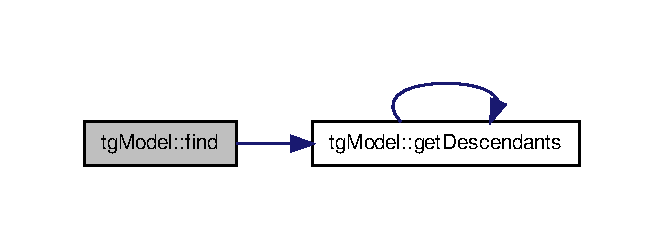
\includegraphics[width=318pt]{classtg_model_ab75836fdfbd9200f165c3b28a19630c0_cgraph}
\end{center}
\end{figure}


\hypertarget{classtg_model_aa40b5fb32f8941e04d537f4e6c6db35c}{\index{Connector\-Test\-Model@{Connector\-Test\-Model}!find@{find}}
\index{find@{find}!ConnectorTestModel@{Connector\-Test\-Model}}
\subsubsection[{find}]{\setlength{\rightskip}{0pt plus 5cm}template$<$typename T $>$ std\-::vector$<$T$\ast$$>$ tg\-Model\-::find (
\begin{DoxyParamCaption}
\item[{const std\-::string \&}]{tag\-Search}
\end{DoxyParamCaption}
)\hspace{0.3cm}{\ttfamily [inline]}, {\ttfamily [inherited]}}}\label{classtg_model_aa40b5fb32f8941e04d537f4e6c6db35c}
Get a vector of descendants sorted by type and a tagsearch. Useful for pulling out muscle groups, or similar. 
\begin{DoxyParams}[1]{Parameters}
\mbox{\tt in}  & {\em tag\-Search,a} & std\-::string\& that contains the desired tags \\
\hline
\end{DoxyParams}
\begin{DoxyReturn}{Returns}
a std\-::vector of pointers to members that match the tag search and typename T 
\end{DoxyReturn}


Definition at line 142 of file tg\-Model.\-h.



Here is the call graph for this function\-:\nopagebreak
\begin{figure}[H]
\begin{center}
\leavevmode
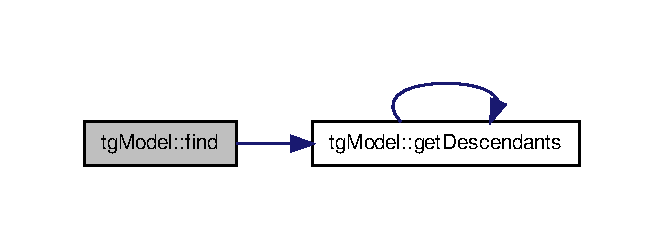
\includegraphics[width=318pt]{classtg_model_aa40b5fb32f8941e04d537f4e6c6db35c_cgraph}
\end{center}
\end{figure}


\hypertarget{classtg_model_a2efa4321fa5c77b4ce23b01f6fd3a1c4}{\index{Connector\-Test\-Model@{Connector\-Test\-Model}!get\-Descendants@{get\-Descendants}}
\index{get\-Descendants@{get\-Descendants}!ConnectorTestModel@{Connector\-Test\-Model}}
\subsubsection[{get\-Descendants}]{\setlength{\rightskip}{0pt plus 5cm}std\-::vector$<$ {\bf tg\-Model} $\ast$ $>$ tg\-Model\-::get\-Descendants (
\begin{DoxyParamCaption}
{}
\end{DoxyParamCaption}
) const\hspace{0.3cm}{\ttfamily [inherited]}}}\label{classtg_model_a2efa4321fa5c77b4ce23b01f6fd3a1c4}
Return a std\-::vector of const pointers to all sub-\/models. \begin{DoxyRefDesc}{Todo}
\item[\hyperlink{todo__todo000017}{Todo}]examine whether this should be public, and perhaps create a read only version \end{DoxyRefDesc}
\begin{DoxyReturn}{Returns}
a std\-::vector of const pointers all sub-\/models.
\end{DoxyReturn}
\begin{DoxyRefDesc}{Todo}
\item[\hyperlink{todo__todo000014}{Todo}]Unnecessary copying can be avoided by pasing the result collection in the recursive step. \end{DoxyRefDesc}


Definition at line 174 of file tg\-Model.\-cpp.



Here is the call graph for this function\-:\nopagebreak
\begin{figure}[H]
\begin{center}
\leavevmode
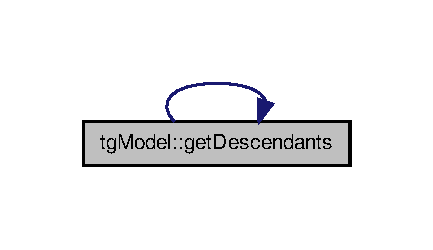
\includegraphics[width=208pt]{classtg_model_a2efa4321fa5c77b4ce23b01f6fd3a1c4_cgraph}
\end{center}
\end{figure}


\hypertarget{classtg_subject_a80799e5d0c8512d3d05a55764790392b}{\index{Connector\-Test\-Model@{Connector\-Test\-Model}!notify\-Setup@{notify\-Setup}}
\index{notify\-Setup@{notify\-Setup}!ConnectorTestModel@{Connector\-Test\-Model}}
\subsubsection[{notify\-Setup}]{\setlength{\rightskip}{0pt plus 5cm}void {\bf tg\-Subject}$<$ {\bf Connector\-Test\-Model}  $>$\-::notify\-Setup (
\begin{DoxyParamCaption}
{}
\end{DoxyParamCaption}
)\hspace{0.3cm}{\ttfamily [inherited]}}}\label{classtg_subject_a80799e5d0c8512d3d05a55764790392b}
Call \hyperlink{classtg_observer_ae7b2de87bd4a6e786bc16f1b801c36a6}{tg\-Observer$<$\-T$>$\-::on\-Setup()} on all observers in the order in which they were attached. \hypertarget{classtg_subject_ad9640aa7fcc1e0b4ce8a913a4ce1ea42}{\index{Connector\-Test\-Model@{Connector\-Test\-Model}!notify\-Step@{notify\-Step}}
\index{notify\-Step@{notify\-Step}!ConnectorTestModel@{Connector\-Test\-Model}}
\subsubsection[{notify\-Step}]{\setlength{\rightskip}{0pt plus 5cm}void {\bf tg\-Subject}$<$ {\bf Connector\-Test\-Model}  $>$\-::notify\-Step (
\begin{DoxyParamCaption}
\item[{double}]{dt}
\end{DoxyParamCaption}
)\hspace{0.3cm}{\ttfamily [inherited]}}}\label{classtg_subject_ad9640aa7fcc1e0b4ce8a913a4ce1ea42}
Call \hyperlink{classtg_observer_a6db5ef1e2792102b8e36dbad5e1a3d7a}{tg\-Observer$<$\-T$>$\-::on\-Step()} on all observers in the order in which they were attached. 
\begin{DoxyParams}[1]{Parameters}
\mbox{\tt in}  & {\em dt} & the number of seconds since the previous call; do nothing if not positive \\
\hline
\end{DoxyParams}


Here is the caller graph for this function\-:
\nopagebreak
\begin{figure}[H]
\begin{center}
\leavevmode
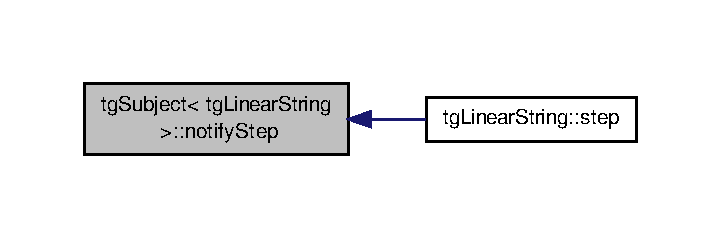
\includegraphics[width=346pt]{classtg_subject_ad9640aa7fcc1e0b4ce8a913a4ce1ea42_icgraph}
\end{center}
\end{figure}


\hypertarget{classtg_subject_adf7a60dbb0faf0de5528f862e7953e63}{\index{Connector\-Test\-Model@{Connector\-Test\-Model}!notify\-Teardown@{notify\-Teardown}}
\index{notify\-Teardown@{notify\-Teardown}!ConnectorTestModel@{Connector\-Test\-Model}}
\subsubsection[{notify\-Teardown}]{\setlength{\rightskip}{0pt plus 5cm}void {\bf tg\-Subject}$<$ {\bf Connector\-Test\-Model}  $>$\-::notify\-Teardown (
\begin{DoxyParamCaption}
{}
\end{DoxyParamCaption}
)\hspace{0.3cm}{\ttfamily [inherited]}}}\label{classtg_subject_adf7a60dbb0faf0de5528f862e7953e63}
Call \hyperlink{classtg_observer_a1663edb3732e5ffb7bbe6bfb4ade88b8}{tg\-Observer$<$\-T$>$\-::on\-Teardown()} on all observers in the order in which they were attached. \hypertarget{class_connector_test_model_a8d4e146eb48dd23676a5522e9417abdb}{\index{Connector\-Test\-Model@{Connector\-Test\-Model}!on\-Visit@{on\-Visit}}
\index{on\-Visit@{on\-Visit}!ConnectorTestModel@{Connector\-Test\-Model}}
\subsubsection[{on\-Visit}]{\setlength{\rightskip}{0pt plus 5cm}virtual void Connector\-Test\-Model\-::on\-Visit (
\begin{DoxyParamCaption}
\item[{const {\bf tg\-Model\-Visitor} \&}]{r}
\end{DoxyParamCaption}
) const\hspace{0.3cm}{\ttfamily [inline]}, {\ttfamily [virtual]}}}\label{class_connector_test_model_a8d4e146eb48dd23676a5522e9417abdb}
Call \hyperlink{classtg_model_visitor_a69d056cf31bb4eeef03c243a86f59cc1}{tg\-Model\-Visitor\-::render()} on self and all descendants. 
\begin{DoxyParams}[1]{Parameters}
\mbox{\tt in,out}  & {\em r} & a reference to a \hyperlink{classtg_model_visitor}{tg\-Model\-Visitor} \\
\hline
\end{DoxyParams}


Reimplemented from \hyperlink{classtg_model_aee6457e0fc54d5570b87bfc779f9b1c0}{tg\-Model}.



Definition at line 152 of file Connector\-Test\-Model.\-h.



Here is the call graph for this function\-:\nopagebreak
\begin{figure}[H]
\begin{center}
\leavevmode
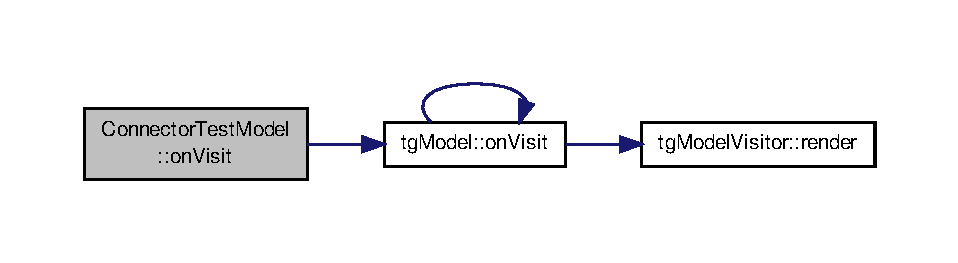
\includegraphics[width=350pt]{class_connector_test_model_a8d4e146eb48dd23676a5522e9417abdb_cgraph}
\end{center}
\end{figure}


\hypertarget{class_connector_test_model_a98cee5085d31f5238dd6c5607eef02bf}{\index{Connector\-Test\-Model@{Connector\-Test\-Model}!setup@{setup}}
\index{setup@{setup}!ConnectorTestModel@{Connector\-Test\-Model}}
\subsubsection[{setup}]{\setlength{\rightskip}{0pt plus 5cm}virtual void Connector\-Test\-Model\-::setup (
\begin{DoxyParamCaption}
\item[{{\bf tg\-World} \&}]{world}
\end{DoxyParamCaption}
)\hspace{0.3cm}{\ttfamily [inline]}, {\ttfamily [virtual]}}}\label{class_connector_test_model_a98cee5085d31f5238dd6c5607eef02bf}
Setup takes a \hyperlink{classtg_world}{tg\-World} and passes it to any children for their own setup functions. All subclasses should call this at the appropriate time (usually end of setup) within their own setup function. 
\begin{DoxyParams}[1]{Parameters}
\mbox{\tt in}  & {\em world} & -\/ the \hyperlink{classtg_world}{tg\-World} the models will exist in. \\
\hline
\end{DoxyParams}


Reimplemented from \hyperlink{classtg_model_a85c68e064972f67c61c47ead392cf6f8}{tg\-Model}.



Definition at line 51 of file Connector\-Test\-Model.\-h.

\hypertarget{class_connector_test_model_a30e5b347373f77dc84584569d8ac7b4e}{\index{Connector\-Test\-Model@{Connector\-Test\-Model}!step@{step}}
\index{step@{step}!ConnectorTestModel@{Connector\-Test\-Model}}
\subsubsection[{step}]{\setlength{\rightskip}{0pt plus 5cm}virtual void Connector\-Test\-Model\-::step (
\begin{DoxyParamCaption}
\item[{double}]{dt}
\end{DoxyParamCaption}
)\hspace{0.3cm}{\ttfamily [inline]}, {\ttfamily [virtual]}}}\label{class_connector_test_model_a30e5b347373f77dc84584569d8ac7b4e}
Advance the simulation. 
\begin{DoxyParams}[1]{Parameters}
\mbox{\tt in}  & {\em dt} & the number of seconds since the previous call; std\-::invalid\-\_\-argument is thrown if dt is not positive \\
\hline
\end{DoxyParams}

\begin{DoxyExceptions}{Exceptions}
{\em std\-::invalid\-\_\-argument} & if dt is not positive \\
\hline
\end{DoxyExceptions}
\begin{DoxyNote}{Note}
This is not necessarily const for every child. 
\end{DoxyNote}


Reimplemented from \hyperlink{classtg_model_acc6f9ae005f9f51447d7efe5f1815737}{tg\-Model}.



Definition at line 140 of file Connector\-Test\-Model.\-h.



Here is the call graph for this function\-:\nopagebreak
\begin{figure}[H]
\begin{center}
\leavevmode
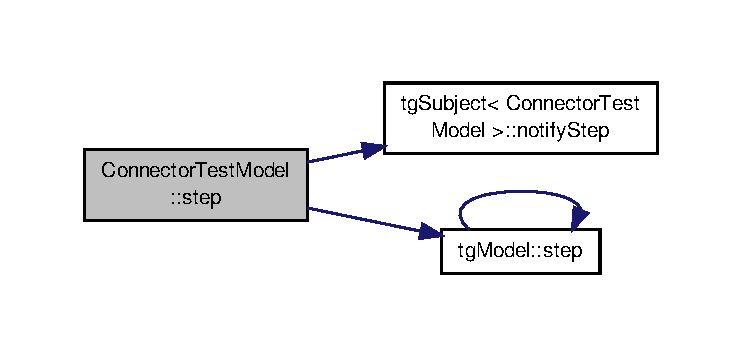
\includegraphics[width=350pt]{class_connector_test_model_a30e5b347373f77dc84584569d8ac7b4e_cgraph}
\end{center}
\end{figure}


\hypertarget{classtg_model_adb5eec1dcf70a8c039850aea144dcc7e}{\index{Connector\-Test\-Model@{Connector\-Test\-Model}!teardown@{teardown}}
\index{teardown@{teardown}!ConnectorTestModel@{Connector\-Test\-Model}}
\subsubsection[{teardown}]{\setlength{\rightskip}{0pt plus 5cm}void tg\-Model\-::teardown (
\begin{DoxyParamCaption}
{}
\end{DoxyParamCaption}
)\hspace{0.3cm}{\ttfamily [virtual]}, {\ttfamily [inherited]}}}\label{classtg_model_adb5eec1dcf70a8c039850aea144dcc7e}
Deletes the children (undoes setup) 

Reimplemented in \hyperlink{classtg_base_string_ae4470639491da403b0a29ef0f11ac7b2}{tg\-Base\-String}, \hyperlink{class_contact_test_model_ad9bf515fa080ba02f1ca304aad47aee9}{Contact\-Test\-Model}, \hyperlink{classtg_rod_a7a12ab9a8190c95c28c2dd6749bb1c8c}{tg\-Rod}, \hyperlink{class_prism_model_ac2b643c26c4e27a27714ea07f274654a}{Prism\-Model}, \hyperlink{classtg_r_b_string_a5f4f77b849a87188569a528937f90a97}{tg\-R\-B\-String}, \hyperlink{classtg_linear_string_a1c4be827e518aa1fc944dd14895b3892}{tg\-Linear\-String}, \hyperlink{class_t6_model_ae46a765cf98ef3b17c4540ee4517c343}{T6\-Model}, \hyperlink{class_spiral_spine_a72bb17d2fabd672ae79dcd80c598303a}{Spiral\-Spine}, \hyperlink{class_base_spine_model_learning_aa04ab240035720769a95c403c1f61f73}{Base\-Spine\-Model\-Learning}, \hyperlink{class_j_early_model_a0883e6fcb262de284dcca1bc91b76154}{J\-Early\-Model}, \hyperlink{class_nested_spiral_spine_aea6ab5feee049adfb73835c848366392}{Nested\-Spiral\-Spine}, \hyperlink{class_flemons_spine_model_learning_a489aeb8529c20f9a2473812ea0e78f41}{Flemons\-Spine\-Model\-Learning}, \hyperlink{class_flemons_spine_model_learning_ab2f98f3230f4980bed706d9337a2fae5}{Flemons\-Spine\-Model\-Learning}, \hyperlink{class_tetra_spine_learning_model_a242f0c007fb565c278a26b4efcc299f4}{Tetra\-Spine\-Learning\-Model}, and \hyperlink{class_rib_model_a1f44d22a7213cd3042383c56dcbac61f}{Rib\-Model}.



Definition at line 73 of file tg\-Model.\-cpp.

\hypertarget{classtg_model_af37b0c1a6d4060bfe0bb9b5038a17725}{\index{Connector\-Test\-Model@{Connector\-Test\-Model}!to\-String@{to\-String}}
\index{to\-String@{to\-String}!ConnectorTestModel@{Connector\-Test\-Model}}
\subsubsection[{to\-String}]{\setlength{\rightskip}{0pt plus 5cm}std\-::string tg\-Model\-::to\-String (
\begin{DoxyParamCaption}
\item[{std\-::string}]{prefix = {\ttfamily \char`\"{}\char`\"{}}}
\end{DoxyParamCaption}
) const\hspace{0.3cm}{\ttfamily [virtual]}, {\ttfamily [inherited]}}}\label{classtg_model_af37b0c1a6d4060bfe0bb9b5038a17725}
Returns the tag names of this model and its children 
\begin{DoxyParams}[1]{Parameters}
\mbox{\tt in}  & {\em prefix} & a string to append to \\
\hline
\end{DoxyParams}
\begin{DoxyReturn}{Returns}
the original string with this model and its children's tags appended 
\end{DoxyReturn}


Definition at line 156 of file tg\-Model.\-cpp.



Here is the caller graph for this function\-:\nopagebreak
\begin{figure}[H]
\begin{center}
\leavevmode
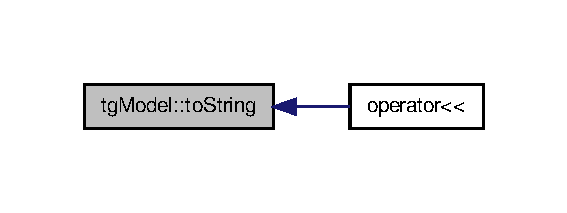
\includegraphics[width=272pt]{classtg_model_af37b0c1a6d4060bfe0bb9b5038a17725_icgraph}
\end{center}
\end{figure}




The documentation for this class was generated from the following file\-:\begin{DoxyCompactItemize}
\item 
dev/tests/Connector\-Test\-Model.\-h\end{DoxyCompactItemize}

\hypertarget{class_contact_test_controller}{\section{Contact\-Test\-Controller Class Reference}
\label{class_contact_test_controller}\index{Contact\-Test\-Controller@{Contact\-Test\-Controller}}
}


Inheritance diagram for Contact\-Test\-Controller\-:\nopagebreak
\begin{figure}[H]
\begin{center}
\leavevmode
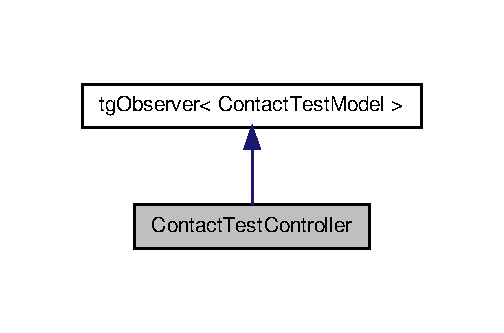
\includegraphics[width=242pt]{class_contact_test_controller__inherit__graph}
\end{center}
\end{figure}


Collaboration diagram for Contact\-Test\-Controller\-:\nopagebreak
\begin{figure}[H]
\begin{center}
\leavevmode
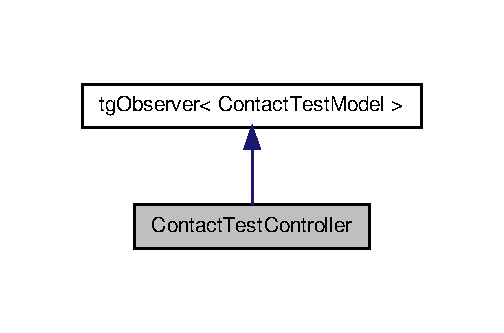
\includegraphics[width=242pt]{class_contact_test_controller__coll__graph}
\end{center}
\end{figure}
\subsection*{Public Member Functions}
\begin{DoxyCompactItemize}
\item 
virtual void \hyperlink{class_contact_test_controller_ac66f0ea2e87ccd2512ad0fb5bfd61208}{on\-Step} (\hyperlink{class_contact_test_model}{Contact\-Test\-Model} \&subject, double dt)
\item 
virtual void \hyperlink{classtg_observer_a0ecd07483eb41f9a0ab19b8ed24052f1}{on\-Attach} (\hyperlink{class_contact_test_model}{Contact\-Test\-Model} \&subject)
\item 
virtual void \hyperlink{classtg_observer_ae7b2de87bd4a6e786bc16f1b801c36a6}{on\-Setup} (\hyperlink{class_contact_test_model}{Contact\-Test\-Model} \&subject)
\item 
virtual void \hyperlink{classtg_observer_a1663edb3732e5ffb7bbe6bfb4ade88b8}{on\-Teardown} (\hyperlink{class_contact_test_model}{Contact\-Test\-Model} \&subject)
\end{DoxyCompactItemize}


\subsection{Detailed Description}


Definition at line 29 of file Contact\-Test\-Controller.\-h.



\subsection{Member Function Documentation}
\hypertarget{classtg_observer_a0ecd07483eb41f9a0ab19b8ed24052f1}{\index{Contact\-Test\-Controller@{Contact\-Test\-Controller}!on\-Attach@{on\-Attach}}
\index{on\-Attach@{on\-Attach}!ContactTestController@{Contact\-Test\-Controller}}
\subsubsection[{on\-Attach}]{\setlength{\rightskip}{0pt plus 5cm}virtual void {\bf tg\-Observer}$<$ {\bf Contact\-Test\-Model}  $>$\-::on\-Attach (
\begin{DoxyParamCaption}
\item[{{\bf Contact\-Test\-Model}  \&}]{subject}
\end{DoxyParamCaption}
)\hspace{0.3cm}{\ttfamily [inline]}, {\ttfamily [virtual]}, {\ttfamily [inherited]}}}\label{classtg_observer_a0ecd07483eb41f9a0ab19b8ed24052f1}
Notify the observers when an attach action has occurred. Will only occur once, typically before setup 
\begin{DoxyParams}[1]{Parameters}
\mbox{\tt in,out}  & {\em subject} & the subject being observed \\
\hline
\end{DoxyParams}


Definition at line 54 of file tg\-Observer.\-h.

\hypertarget{classtg_observer_ae7b2de87bd4a6e786bc16f1b801c36a6}{\index{Contact\-Test\-Controller@{Contact\-Test\-Controller}!on\-Setup@{on\-Setup}}
\index{on\-Setup@{on\-Setup}!ContactTestController@{Contact\-Test\-Controller}}
\subsubsection[{on\-Setup}]{\setlength{\rightskip}{0pt plus 5cm}virtual void {\bf tg\-Observer}$<$ {\bf Contact\-Test\-Model}  $>$\-::on\-Setup (
\begin{DoxyParamCaption}
\item[{{\bf Contact\-Test\-Model}  \&}]{subject}
\end{DoxyParamCaption}
)\hspace{0.3cm}{\ttfamily [inline]}, {\ttfamily [virtual]}, {\ttfamily [inherited]}}}\label{classtg_observer_ae7b2de87bd4a6e786bc16f1b801c36a6}
Notify the observers when a setup action has occurred. 
\begin{DoxyParams}[1]{Parameters}
\mbox{\tt in,out}  & {\em subject} & the subject being observed \\
\hline
\end{DoxyParams}


Definition at line 60 of file tg\-Observer.\-h.

\hypertarget{class_contact_test_controller_ac66f0ea2e87ccd2512ad0fb5bfd61208}{\index{Contact\-Test\-Controller@{Contact\-Test\-Controller}!on\-Step@{on\-Step}}
\index{on\-Step@{on\-Step}!ContactTestController@{Contact\-Test\-Controller}}
\subsubsection[{on\-Step}]{\setlength{\rightskip}{0pt plus 5cm}virtual void Contact\-Test\-Controller\-::on\-Step (
\begin{DoxyParamCaption}
\item[{{\bf Contact\-Test\-Model} \&}]{subject, }
\item[{double}]{dt}
\end{DoxyParamCaption}
)\hspace{0.3cm}{\ttfamily [inline]}, {\ttfamily [virtual]}}}\label{class_contact_test_controller_ac66f0ea2e87ccd2512ad0fb5bfd61208}
Notify the observers when a step action has occurred. 
\begin{DoxyParams}[1]{Parameters}
\mbox{\tt in,out}  & {\em subject} & the subject being observed \\
\hline
\mbox{\tt in}  & {\em the} & number of seconds since the previous call; must be positive \\
\hline
\end{DoxyParams}


Implements \hyperlink{classtg_observer_a6db5ef1e2792102b8e36dbad5e1a3d7a}{tg\-Observer$<$ Contact\-Test\-Model $>$}.



Definition at line 37 of file Contact\-Test\-Controller.\-h.



Here is the call graph for this function\-:\nopagebreak
\begin{figure}[H]
\begin{center}
\leavevmode
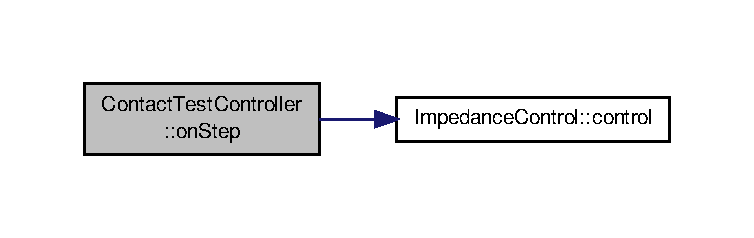
\includegraphics[width=350pt]{class_contact_test_controller_ac66f0ea2e87ccd2512ad0fb5bfd61208_cgraph}
\end{center}
\end{figure}


\hypertarget{classtg_observer_a1663edb3732e5ffb7bbe6bfb4ade88b8}{\index{Contact\-Test\-Controller@{Contact\-Test\-Controller}!on\-Teardown@{on\-Teardown}}
\index{on\-Teardown@{on\-Teardown}!ContactTestController@{Contact\-Test\-Controller}}
\subsubsection[{on\-Teardown}]{\setlength{\rightskip}{0pt plus 5cm}virtual void {\bf tg\-Observer}$<$ {\bf Contact\-Test\-Model}  $>$\-::on\-Teardown (
\begin{DoxyParamCaption}
\item[{{\bf Contact\-Test\-Model}  \&}]{subject}
\end{DoxyParamCaption}
)\hspace{0.3cm}{\ttfamily [inline]}, {\ttfamily [virtual]}, {\ttfamily [inherited]}}}\label{classtg_observer_a1663edb3732e5ffb7bbe6bfb4ade88b8}
Notify the observers when a teardown action has occurred. 
\begin{DoxyParams}[1]{Parameters}
\mbox{\tt in,out}  & {\em subject} & the subject being observed \\
\hline
\end{DoxyParams}


Definition at line 66 of file tg\-Observer.\-h.



The documentation for this class was generated from the following file\-:\begin{DoxyCompactItemize}
\item 
dev/btietz/\-R\-B\-Tests/Contact\-Test\-Controller.\-h\end{DoxyCompactItemize}

\hypertarget{class_contact_test_model}{\section{Contact\-Test\-Model Class Reference}
\label{class_contact_test_model}\index{Contact\-Test\-Model@{Contact\-Test\-Model}}
}


Inheritance diagram for Contact\-Test\-Model\-:\nopagebreak
\begin{figure}[H]
\begin{center}
\leavevmode
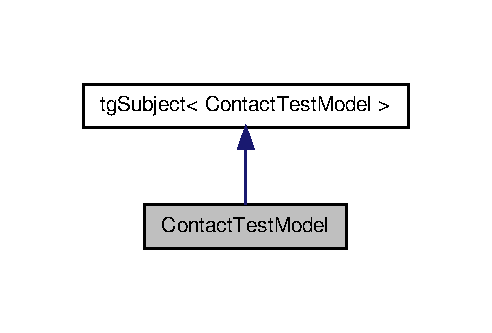
\includegraphics[width=236pt]{class_contact_test_model__inherit__graph}
\end{center}
\end{figure}


Collaboration diagram for Contact\-Test\-Model\-:\nopagebreak
\begin{figure}[H]
\begin{center}
\leavevmode
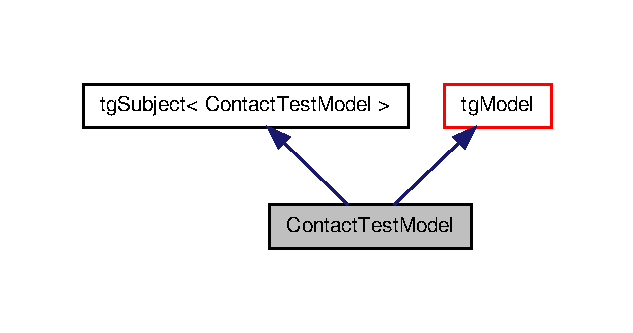
\includegraphics[width=304pt]{class_contact_test_model__coll__graph}
\end{center}
\end{figure}
\subsection*{Public Member Functions}
\begin{DoxyCompactItemize}
\item 
virtual void \hyperlink{class_contact_test_model_a9bebeeb19f836cb456aa187a76015675}{setup} (\hyperlink{classtg_world}{tg\-World} \&world)
\item 
virtual void \hyperlink{class_contact_test_model_a4ca4c597ea5333b0230fb3f05eebca97}{step} (double dt)
\item 
void \hyperlink{class_contact_test_model_ad9bf515fa080ba02f1ca304aad47aee9}{teardown} ()
\item 
\hypertarget{class_contact_test_model_a3ec6248a546825bde14b2ab316bc6273}{std\-::vector$<$ \hyperlink{classtg_r_b_string}{tg\-R\-B\-String} $\ast$ $>$ \& {\bfseries get\-All\-Muscles} ()}\label{class_contact_test_model_a3ec6248a546825bde14b2ab316bc6273}

\item 
void \hyperlink{classtg_subject_a56ecfd33a048c3a7f1a884318d9af548}{attach} (\hyperlink{classtg_observer}{tg\-Observer}$<$ \hyperlink{class_contact_test_model}{Contact\-Test\-Model} $>$ $\ast$p\-Observer)
\item 
void \hyperlink{classtg_subject_ad9640aa7fcc1e0b4ce8a913a4ce1ea42}{notify\-Step} (double dt)
\item 
void \hyperlink{classtg_subject_a80799e5d0c8512d3d05a55764790392b}{notify\-Setup} ()
\item 
void \hyperlink{classtg_subject_adf7a60dbb0faf0de5528f862e7953e63}{notify\-Teardown} ()
\item 
virtual void \hyperlink{classtg_model_aee6457e0fc54d5570b87bfc779f9b1c0}{on\-Visit} (const \hyperlink{classtg_model_visitor}{tg\-Model\-Visitor} \&r) const 
\item 
void \hyperlink{classtg_model_a292c17848b96caee32b2286e44c13f2f}{add\-Child} (\hyperlink{classtg_model}{tg\-Model} $\ast$p\-Child)
\item 
virtual std\-::string \hyperlink{classtg_model_af37b0c1a6d4060bfe0bb9b5038a17725}{to\-String} (std\-::string prefix=\char`\"{}\char`\"{}) const 
\item 
{\footnotesize template$<$typename T $>$ }\\std\-::vector$<$ T $\ast$ $>$ \hyperlink{classtg_model_ab75836fdfbd9200f165c3b28a19630c0}{find} (const \hyperlink{classtg_tag_search}{tg\-Tag\-Search} \&tag\-Search)
\item 
{\footnotesize template$<$typename T $>$ }\\std\-::vector$<$ T $\ast$ $>$ \hyperlink{classtg_model_aa40b5fb32f8941e04d537f4e6c6db35c}{find} (const std\-::string \&tag\-Search)
\item 
std\-::vector$<$ \hyperlink{classtg_model}{tg\-Model} $\ast$ $>$ \hyperlink{classtg_model_a2efa4321fa5c77b4ce23b01f6fd3a1c4}{get\-Descendants} () const 
\item 
\hypertarget{classtg_taggable_af0b8f1729653b0b90d2fecbd51163612}{void {\bfseries add\-Tags} (const std\-::string \&space\-\_\-separated\-\_\-tags)}\label{classtg_taggable_af0b8f1729653b0b90d2fecbd51163612}

\item 
\hypertarget{classtg_taggable_af28e3fe1a7e4eb28772dc006d575dd1f}{void {\bfseries add\-Tags} (const \hyperlink{classtg_tags}{tg\-Tags} \&tags)}\label{classtg_taggable_af28e3fe1a7e4eb28772dc006d575dd1f}

\item 
\hypertarget{classtg_taggable_ae31f65869c8887bfeb34a344902c4d5b}{bool {\bfseries has\-Tag} (const std\-::string tag) const }\label{classtg_taggable_ae31f65869c8887bfeb34a344902c4d5b}

\item 
\hypertarget{classtg_taggable_a33b77b1075171b63f673965687b2e844}{bool {\bfseries has\-All\-Tags} (std\-::string tags)}\label{classtg_taggable_a33b77b1075171b63f673965687b2e844}

\item 
\hypertarget{classtg_taggable_af14af28fa98021c4f20a5e8f2ddd5606}{bool {\bfseries has\-Any\-Tags} (const std\-::string tags)}\label{classtg_taggable_af14af28fa98021c4f20a5e8f2ddd5606}

\item 
\hypertarget{classtg_taggable_adff345e116e16420c701a748ff8f995f}{bool {\bfseries has\-No\-Tags} ()}\label{classtg_taggable_adff345e116e16420c701a748ff8f995f}

\item 
\hypertarget{classtg_taggable_acf1d7fa9df8f374f25015c4080902681}{\hyperlink{classtg_tags}{tg\-Tags} \& {\bfseries get\-Tags} ()}\label{classtg_taggable_acf1d7fa9df8f374f25015c4080902681}

\item 
\hypertarget{classtg_taggable_ae70d7d3b45301665bc363b0ed8b9b292}{const \hyperlink{classtg_tags}{tg\-Tags} \& {\bfseries get\-Tags} () const }\label{classtg_taggable_ae70d7d3b45301665bc363b0ed8b9b292}

\item 
\hypertarget{classtg_taggable_a5492888e4e4da4cca6261070b5726adf}{void {\bfseries set\-Tags} (\hyperlink{classtg_tags}{tg\-Tags} tags)}\label{classtg_taggable_a5492888e4e4da4cca6261070b5726adf}

\item 
\hypertarget{classtg_taggable_a346d66b066d2d9eb1eadba01da43749f}{std\-::string {\bfseries get\-Tag\-Str} (std\-::string delim=\char`\"{} \char`\"{}) const }\label{classtg_taggable_a346d66b066d2d9eb1eadba01da43749f}

\end{DoxyCompactItemize}


\subsection{Detailed Description}


Definition at line 46 of file Contact\-Test\-Model.\-h.



\subsection{Member Function Documentation}
\hypertarget{classtg_model_a292c17848b96caee32b2286e44c13f2f}{\index{Contact\-Test\-Model@{Contact\-Test\-Model}!add\-Child@{add\-Child}}
\index{add\-Child@{add\-Child}!ContactTestModel@{Contact\-Test\-Model}}
\subsubsection[{add\-Child}]{\setlength{\rightskip}{0pt plus 5cm}void tg\-Model\-::add\-Child (
\begin{DoxyParamCaption}
\item[{{\bf tg\-Model} $\ast$}]{p\-Child}
\end{DoxyParamCaption}
)\hspace{0.3cm}{\ttfamily [inherited]}}}\label{classtg_model_a292c17848b96caee32b2286e44c13f2f}
Add a sub-\/model to this model. The model takes ownership of the child sub-\/model and is responsible for deallocating it. 
\begin{DoxyParams}[1]{Parameters}
\mbox{\tt in,out}  & {\em p\-Child} & a pointer to a sub-\/model \\
\hline
\end{DoxyParams}

\begin{DoxyExceptions}{Exceptions}
{\em std\-::invalid\-\_\-argument} & is p\-Child is N\-U\-L\-L, this object, or already a descendant \\
\hline
\end{DoxyExceptions}
\begin{DoxyRefDesc}{Todo}
\item[\hyperlink{todo__todo000016}{Todo}]Make sure that every child appears no more than once in the tree. \end{DoxyRefDesc}


Definition at line 126 of file tg\-Model.\-cpp.



Here is the call graph for this function\-:\nopagebreak
\begin{figure}[H]
\begin{center}
\leavevmode
\includegraphics[width=340pt]{classtg_model_a292c17848b96caee32b2286e44c13f2f_cgraph}
\end{center}
\end{figure}




Here is the caller graph for this function\-:\nopagebreak
\begin{figure}[H]
\begin{center}
\leavevmode
\includegraphics[width=320pt]{classtg_model_a292c17848b96caee32b2286e44c13f2f_icgraph}
\end{center}
\end{figure}


\hypertarget{classtg_subject_a56ecfd33a048c3a7f1a884318d9af548}{\index{Contact\-Test\-Model@{Contact\-Test\-Model}!attach@{attach}}
\index{attach@{attach}!ContactTestModel@{Contact\-Test\-Model}}
\subsubsection[{attach}]{\setlength{\rightskip}{0pt plus 5cm}void {\bf tg\-Subject}$<$ {\bf Contact\-Test\-Model}  $>$\-::attach (
\begin{DoxyParamCaption}
\item[{{\bf tg\-Observer}$<$ {\bf Contact\-Test\-Model}  $>$ $\ast$}]{p\-Observer}
\end{DoxyParamCaption}
)\hspace{0.3cm}{\ttfamily [inherited]}}}\label{classtg_subject_a56ecfd33a048c3a7f1a884318d9af548}
Attach an observer to the subject of the observer. 
\begin{DoxyParams}[1]{Parameters}
\mbox{\tt in,out}  & {\em p\-Observer} & a pointer to an observer for the subject; do nothing if the pointer is N\-U\-L\-L \\
\hline
\end{DoxyParams}
\hypertarget{classtg_model_ab75836fdfbd9200f165c3b28a19630c0}{\index{Contact\-Test\-Model@{Contact\-Test\-Model}!find@{find}}
\index{find@{find}!ContactTestModel@{Contact\-Test\-Model}}
\subsubsection[{find}]{\setlength{\rightskip}{0pt plus 5cm}template$<$typename T $>$ std\-::vector$<$T$\ast$$>$ tg\-Model\-::find (
\begin{DoxyParamCaption}
\item[{const {\bf tg\-Tag\-Search} \&}]{tag\-Search}
\end{DoxyParamCaption}
)\hspace{0.3cm}{\ttfamily [inline]}, {\ttfamily [inherited]}}}\label{classtg_model_ab75836fdfbd9200f165c3b28a19630c0}
Get a vector of descendants sorted by type and a tagsearch. Useful for pulling out muscle groups, or similar. 
\begin{DoxyParams}[1]{Parameters}
\mbox{\tt in}  & {\em tag\-Search,a} & tag\-Search that contains the desired tags \\
\hline
\end{DoxyParams}
\begin{DoxyReturn}{Returns}
a std\-::vector of pointers to members that match the tag search and typename T 
\end{DoxyReturn}


Definition at line 129 of file tg\-Model.\-h.



Here is the call graph for this function\-:\nopagebreak
\begin{figure}[H]
\begin{center}
\leavevmode
\includegraphics[width=318pt]{classtg_model_ab75836fdfbd9200f165c3b28a19630c0_cgraph}
\end{center}
\end{figure}


\hypertarget{classtg_model_aa40b5fb32f8941e04d537f4e6c6db35c}{\index{Contact\-Test\-Model@{Contact\-Test\-Model}!find@{find}}
\index{find@{find}!ContactTestModel@{Contact\-Test\-Model}}
\subsubsection[{find}]{\setlength{\rightskip}{0pt plus 5cm}template$<$typename T $>$ std\-::vector$<$T$\ast$$>$ tg\-Model\-::find (
\begin{DoxyParamCaption}
\item[{const std\-::string \&}]{tag\-Search}
\end{DoxyParamCaption}
)\hspace{0.3cm}{\ttfamily [inline]}, {\ttfamily [inherited]}}}\label{classtg_model_aa40b5fb32f8941e04d537f4e6c6db35c}
Get a vector of descendants sorted by type and a tagsearch. Useful for pulling out muscle groups, or similar. 
\begin{DoxyParams}[1]{Parameters}
\mbox{\tt in}  & {\em tag\-Search,a} & std\-::string\& that contains the desired tags \\
\hline
\end{DoxyParams}
\begin{DoxyReturn}{Returns}
a std\-::vector of pointers to members that match the tag search and typename T 
\end{DoxyReturn}


Definition at line 142 of file tg\-Model.\-h.



Here is the call graph for this function\-:\nopagebreak
\begin{figure}[H]
\begin{center}
\leavevmode
\includegraphics[width=318pt]{classtg_model_aa40b5fb32f8941e04d537f4e6c6db35c_cgraph}
\end{center}
\end{figure}


\hypertarget{classtg_model_a2efa4321fa5c77b4ce23b01f6fd3a1c4}{\index{Contact\-Test\-Model@{Contact\-Test\-Model}!get\-Descendants@{get\-Descendants}}
\index{get\-Descendants@{get\-Descendants}!ContactTestModel@{Contact\-Test\-Model}}
\subsubsection[{get\-Descendants}]{\setlength{\rightskip}{0pt plus 5cm}std\-::vector$<$ {\bf tg\-Model} $\ast$ $>$ tg\-Model\-::get\-Descendants (
\begin{DoxyParamCaption}
{}
\end{DoxyParamCaption}
) const\hspace{0.3cm}{\ttfamily [inherited]}}}\label{classtg_model_a2efa4321fa5c77b4ce23b01f6fd3a1c4}
Return a std\-::vector of const pointers to all sub-\/models. \begin{DoxyRefDesc}{Todo}
\item[\hyperlink{todo__todo000017}{Todo}]examine whether this should be public, and perhaps create a read only version \end{DoxyRefDesc}
\begin{DoxyReturn}{Returns}
a std\-::vector of const pointers all sub-\/models.
\end{DoxyReturn}
\begin{DoxyRefDesc}{Todo}
\item[\hyperlink{todo__todo000014}{Todo}]Unnecessary copying can be avoided by pasing the result collection in the recursive step. \end{DoxyRefDesc}


Definition at line 174 of file tg\-Model.\-cpp.



Here is the call graph for this function\-:\nopagebreak
\begin{figure}[H]
\begin{center}
\leavevmode
\includegraphics[width=208pt]{classtg_model_a2efa4321fa5c77b4ce23b01f6fd3a1c4_cgraph}
\end{center}
\end{figure}


\hypertarget{classtg_subject_a80799e5d0c8512d3d05a55764790392b}{\index{Contact\-Test\-Model@{Contact\-Test\-Model}!notify\-Setup@{notify\-Setup}}
\index{notify\-Setup@{notify\-Setup}!ContactTestModel@{Contact\-Test\-Model}}
\subsubsection[{notify\-Setup}]{\setlength{\rightskip}{0pt plus 5cm}void {\bf tg\-Subject}$<$ {\bf Contact\-Test\-Model}  $>$\-::notify\-Setup (
\begin{DoxyParamCaption}
{}
\end{DoxyParamCaption}
)\hspace{0.3cm}{\ttfamily [inherited]}}}\label{classtg_subject_a80799e5d0c8512d3d05a55764790392b}
Call \hyperlink{classtg_observer_ae7b2de87bd4a6e786bc16f1b801c36a6}{tg\-Observer$<$\-T$>$\-::on\-Setup()} on all observers in the order in which they were attached. \hypertarget{classtg_subject_ad9640aa7fcc1e0b4ce8a913a4ce1ea42}{\index{Contact\-Test\-Model@{Contact\-Test\-Model}!notify\-Step@{notify\-Step}}
\index{notify\-Step@{notify\-Step}!ContactTestModel@{Contact\-Test\-Model}}
\subsubsection[{notify\-Step}]{\setlength{\rightskip}{0pt plus 5cm}void {\bf tg\-Subject}$<$ {\bf Contact\-Test\-Model}  $>$\-::notify\-Step (
\begin{DoxyParamCaption}
\item[{double}]{dt}
\end{DoxyParamCaption}
)\hspace{0.3cm}{\ttfamily [inherited]}}}\label{classtg_subject_ad9640aa7fcc1e0b4ce8a913a4ce1ea42}
Call \hyperlink{classtg_observer_a6db5ef1e2792102b8e36dbad5e1a3d7a}{tg\-Observer$<$\-T$>$\-::on\-Step()} on all observers in the order in which they were attached. 
\begin{DoxyParams}[1]{Parameters}
\mbox{\tt in}  & {\em dt} & the number of seconds since the previous call; do nothing if not positive \\
\hline
\end{DoxyParams}


Here is the caller graph for this function\-:
\nopagebreak
\begin{figure}[H]
\begin{center}
\leavevmode
\includegraphics[width=346pt]{classtg_subject_ad9640aa7fcc1e0b4ce8a913a4ce1ea42_icgraph}
\end{center}
\end{figure}


\hypertarget{classtg_subject_adf7a60dbb0faf0de5528f862e7953e63}{\index{Contact\-Test\-Model@{Contact\-Test\-Model}!notify\-Teardown@{notify\-Teardown}}
\index{notify\-Teardown@{notify\-Teardown}!ContactTestModel@{Contact\-Test\-Model}}
\subsubsection[{notify\-Teardown}]{\setlength{\rightskip}{0pt plus 5cm}void {\bf tg\-Subject}$<$ {\bf Contact\-Test\-Model}  $>$\-::notify\-Teardown (
\begin{DoxyParamCaption}
{}
\end{DoxyParamCaption}
)\hspace{0.3cm}{\ttfamily [inherited]}}}\label{classtg_subject_adf7a60dbb0faf0de5528f862e7953e63}
Call \hyperlink{classtg_observer_a1663edb3732e5ffb7bbe6bfb4ade88b8}{tg\-Observer$<$\-T$>$\-::on\-Teardown()} on all observers in the order in which they were attached. \hypertarget{classtg_model_aee6457e0fc54d5570b87bfc779f9b1c0}{\index{Contact\-Test\-Model@{Contact\-Test\-Model}!on\-Visit@{on\-Visit}}
\index{on\-Visit@{on\-Visit}!ContactTestModel@{Contact\-Test\-Model}}
\subsubsection[{on\-Visit}]{\setlength{\rightskip}{0pt plus 5cm}void tg\-Model\-::on\-Visit (
\begin{DoxyParamCaption}
\item[{const {\bf tg\-Model\-Visitor} \&}]{r}
\end{DoxyParamCaption}
) const\hspace{0.3cm}{\ttfamily [virtual]}, {\ttfamily [inherited]}}}\label{classtg_model_aee6457e0fc54d5570b87bfc779f9b1c0}
Call \hyperlink{classtg_model_visitor_a69d056cf31bb4eeef03c243a86f59cc1}{tg\-Model\-Visitor\-::render()} on self and all descendants. 
\begin{DoxyParams}[1]{Parameters}
\mbox{\tt in,out}  & {\em r} & a reference to a \hyperlink{classtg_model_visitor}{tg\-Model\-Visitor} \\
\hline
\end{DoxyParams}


Reimplemented in \hyperlink{class_connector_test_model_a8d4e146eb48dd23676a5522e9417abdb}{Connector\-Test\-Model}, \hyperlink{class_build_test_model_a8f12c5e787faba7606bbd46531819a4b}{Build\-Test\-Model}, \hyperlink{classtg_linear_string_a9f659486ba4276dc9d60982158fb7aa5}{tg\-Linear\-String}, and \hyperlink{classtg_rod_ae3651ef650b66a5d016bc5ffb27ec449}{tg\-Rod}.



Definition at line 109 of file tg\-Model.\-cpp.



Here is the call graph for this function\-:\nopagebreak
\begin{figure}[H]
\begin{center}
\leavevmode
\includegraphics[width=316pt]{classtg_model_aee6457e0fc54d5570b87bfc779f9b1c0_cgraph}
\end{center}
\end{figure}


\hypertarget{class_contact_test_model_a9bebeeb19f836cb456aa187a76015675}{\index{Contact\-Test\-Model@{Contact\-Test\-Model}!setup@{setup}}
\index{setup@{setup}!ContactTestModel@{Contact\-Test\-Model}}
\subsubsection[{setup}]{\setlength{\rightskip}{0pt plus 5cm}virtual void Contact\-Test\-Model\-::setup (
\begin{DoxyParamCaption}
\item[{{\bf tg\-World} \&}]{world}
\end{DoxyParamCaption}
)\hspace{0.3cm}{\ttfamily [inline]}, {\ttfamily [virtual]}}}\label{class_contact_test_model_a9bebeeb19f836cb456aa187a76015675}
\begin{DoxyRefDesc}{Todo}
\item[\hyperlink{todo__todo000042}{Todo}]Get rid of this. \end{DoxyRefDesc}


Reimplemented from \hyperlink{classtg_model_a85c68e064972f67c61c47ead392cf6f8}{tg\-Model}.



Definition at line 58 of file Contact\-Test\-Model.\-h.

\hypertarget{class_contact_test_model_a4ca4c597ea5333b0230fb3f05eebca97}{\index{Contact\-Test\-Model@{Contact\-Test\-Model}!step@{step}}
\index{step@{step}!ContactTestModel@{Contact\-Test\-Model}}
\subsubsection[{step}]{\setlength{\rightskip}{0pt plus 5cm}virtual void Contact\-Test\-Model\-::step (
\begin{DoxyParamCaption}
\item[{double}]{dt}
\end{DoxyParamCaption}
)\hspace{0.3cm}{\ttfamily [inline]}, {\ttfamily [virtual]}}}\label{class_contact_test_model_a4ca4c597ea5333b0230fb3f05eebca97}
Advance the simulation. 
\begin{DoxyParams}[1]{Parameters}
\mbox{\tt in}  & {\em dt} & the number of seconds since the previous call; std\-::invalid\-\_\-argument is thrown if dt is not positive \\
\hline
\end{DoxyParams}

\begin{DoxyExceptions}{Exceptions}
{\em std\-::invalid\-\_\-argument} & if dt is not positive \\
\hline
\end{DoxyExceptions}
\begin{DoxyNote}{Note}
This is not necessarily const for every child. 
\end{DoxyNote}


Reimplemented from \hyperlink{classtg_model_acc6f9ae005f9f51447d7efe5f1815737}{tg\-Model}.



Definition at line 133 of file Contact\-Test\-Model.\-h.



Here is the call graph for this function\-:\nopagebreak
\begin{figure}[H]
\begin{center}
\leavevmode
\includegraphics[width=350pt]{class_contact_test_model_a4ca4c597ea5333b0230fb3f05eebca97_cgraph}
\end{center}
\end{figure}


\hypertarget{class_contact_test_model_ad9bf515fa080ba02f1ca304aad47aee9}{\index{Contact\-Test\-Model@{Contact\-Test\-Model}!teardown@{teardown}}
\index{teardown@{teardown}!ContactTestModel@{Contact\-Test\-Model}}
\subsubsection[{teardown}]{\setlength{\rightskip}{0pt plus 5cm}void Contact\-Test\-Model\-::teardown (
\begin{DoxyParamCaption}
{}
\end{DoxyParamCaption}
)\hspace{0.3cm}{\ttfamily [inline]}, {\ttfamily [virtual]}}}\label{class_contact_test_model_ad9bf515fa080ba02f1ca304aad47aee9}
Deletes the children (undoes setup) 

Reimplemented from \hyperlink{classtg_model_adb5eec1dcf70a8c039850aea144dcc7e}{tg\-Model}.



Definition at line 142 of file Contact\-Test\-Model.\-h.



Here is the call graph for this function\-:\nopagebreak
\begin{figure}[H]
\begin{center}
\leavevmode
\includegraphics[width=350pt]{class_contact_test_model_ad9bf515fa080ba02f1ca304aad47aee9_cgraph}
\end{center}
\end{figure}


\hypertarget{classtg_model_af37b0c1a6d4060bfe0bb9b5038a17725}{\index{Contact\-Test\-Model@{Contact\-Test\-Model}!to\-String@{to\-String}}
\index{to\-String@{to\-String}!ContactTestModel@{Contact\-Test\-Model}}
\subsubsection[{to\-String}]{\setlength{\rightskip}{0pt plus 5cm}std\-::string tg\-Model\-::to\-String (
\begin{DoxyParamCaption}
\item[{std\-::string}]{prefix = {\ttfamily \char`\"{}\char`\"{}}}
\end{DoxyParamCaption}
) const\hspace{0.3cm}{\ttfamily [virtual]}, {\ttfamily [inherited]}}}\label{classtg_model_af37b0c1a6d4060bfe0bb9b5038a17725}
Returns the tag names of this model and its children 
\begin{DoxyParams}[1]{Parameters}
\mbox{\tt in}  & {\em prefix} & a string to append to \\
\hline
\end{DoxyParams}
\begin{DoxyReturn}{Returns}
the original string with this model and its children's tags appended 
\end{DoxyReturn}


Definition at line 156 of file tg\-Model.\-cpp.



Here is the caller graph for this function\-:\nopagebreak
\begin{figure}[H]
\begin{center}
\leavevmode
\includegraphics[width=272pt]{classtg_model_af37b0c1a6d4060bfe0bb9b5038a17725_icgraph}
\end{center}
\end{figure}




The documentation for this class was generated from the following file\-:\begin{DoxyCompactItemize}
\item 
dev/btietz/\-R\-B\-Tests/Contact\-Test\-Model.\-h\end{DoxyCompactItemize}

\hypertarget{class_c_p_g_edge}{\section{C\-P\-G\-Edge Class Reference}
\label{class_c_p_g_edge}\index{C\-P\-G\-Edge@{C\-P\-G\-Edge}}
}


Collaboration diagram for C\-P\-G\-Edge\-:\nopagebreak
\begin{figure}[H]
\begin{center}
\leavevmode
\includegraphics[width=163pt]{class_c_p_g_edge__coll__graph}
\end{center}
\end{figure}
\subsection*{Public Member Functions}
\begin{DoxyCompactItemize}
\item 
\hypertarget{class_c_p_g_edge_afb98365a70af9a064abfc9d4167bb3f7}{{\bfseries C\-P\-G\-Edge} (\hyperlink{class_c_p_g_node}{C\-P\-G\-Node} $\ast$new\-Target, double new\-Weight, double new\-Phase)}\label{class_c_p_g_edge_afb98365a70af9a064abfc9d4167bb3f7}

\item 
\hyperlink{class_c_p_g_edge_addf39bbf494c96c60fb5546611414d7a}{$\sim$\-C\-P\-G\-Edge} ()
\item 
virtual void \hyperlink{class_c_p_g_edge_aecea428c30891ef8632192cfe2fa3649}{couple} (\hyperlink{class_c_p_g_node}{C\-P\-G\-Node} \&current\-Node)
\item 
\hypertarget{class_c_p_g_edge_a1f4afbee9e7fa17d2062e5d507574240}{\hyperlink{class_c_p_g_node}{C\-P\-G\-Node} $\ast$ {\bfseries get\-Target\-Node} ()}\label{class_c_p_g_edge_a1f4afbee9e7fa17d2062e5d507574240}

\item 
\hypertarget{class_c_p_g_edge_af80a4916df680b83d391e82390f0f260}{std\-::string {\bfseries to\-String} (const std\-::string \&prefix=\char`\"{}\char`\"{}) const }\label{class_c_p_g_edge_af80a4916df680b83d391e82390f0f260}

\end{DoxyCompactItemize}
\subsection*{Protected Attributes}
\begin{DoxyCompactItemize}
\item 
\hypertarget{class_c_p_g_edge_a33a6ad3f1d477d21ab4030ed4962411d}{\hyperlink{class_c_p_g_node}{C\-P\-G\-Node} $\ast$ {\bfseries target\-Node}}\label{class_c_p_g_edge_a33a6ad3f1d477d21ab4030ed4962411d}

\item 
\hypertarget{class_c_p_g_edge_a910cd71a2ddf2109fbccc7e8bcc8844d}{double {\bfseries weight}}\label{class_c_p_g_edge_a910cd71a2ddf2109fbccc7e8bcc8844d}

\item 
\hypertarget{class_c_p_g_edge_a91801b930b4a29875b0294c0a336976f}{double {\bfseries phase\-Offset}}\label{class_c_p_g_edge_a91801b930b4a29875b0294c0a336976f}

\end{DoxyCompactItemize}


\subsection{Detailed Description}


Definition at line 38 of file C\-P\-G\-Edge.\-h.



\subsection{Constructor \& Destructor Documentation}
\hypertarget{class_c_p_g_edge_addf39bbf494c96c60fb5546611414d7a}{\index{C\-P\-G\-Edge@{C\-P\-G\-Edge}!$\sim$\-C\-P\-G\-Edge@{$\sim$\-C\-P\-G\-Edge}}
\index{$\sim$\-C\-P\-G\-Edge@{$\sim$\-C\-P\-G\-Edge}!CPGEdge@{C\-P\-G\-Edge}}
\subsubsection[{$\sim$\-C\-P\-G\-Edge}]{\setlength{\rightskip}{0pt plus 5cm}C\-P\-G\-Edge\-::$\sim$\-C\-P\-G\-Edge (
\begin{DoxyParamCaption}
{}
\end{DoxyParamCaption}
)}}\label{class_c_p_g_edge_addf39bbf494c96c60fb5546611414d7a}
todo\-: double check cleanup and make sure this needs to delete its nodes 

Definition at line 40 of file C\-P\-G\-Edge.\-cpp.



\subsection{Member Function Documentation}
\hypertarget{class_c_p_g_edge_aecea428c30891ef8632192cfe2fa3649}{\index{C\-P\-G\-Edge@{C\-P\-G\-Edge}!couple@{couple}}
\index{couple@{couple}!CPGEdge@{C\-P\-G\-Edge}}
\subsubsection[{couple}]{\setlength{\rightskip}{0pt plus 5cm}void C\-P\-G\-Edge\-::couple (
\begin{DoxyParamCaption}
\item[{{\bf C\-P\-G\-Node} \&}]{current\-Node}
\end{DoxyParamCaption}
)\hspace{0.3cm}{\ttfamily [virtual]}}}\label{class_c_p_g_edge_aecea428c30891ef8632192cfe2fa3649}
Equation that affects the phase of the node based on the coupled node. Can be overridden to produce a different coupling equation. 

Definition at line 45 of file C\-P\-G\-Edge.\-cpp.



The documentation for this class was generated from the following files\-:\begin{DoxyCompactItemize}
\item 
util/\hyperlink{_c_p_g_edge_8h}{C\-P\-G\-Edge.\-h}\item 
util/\hyperlink{_c_p_g_edge_8cpp}{C\-P\-G\-Edge.\-cpp}\end{DoxyCompactItemize}

\hypertarget{class_c_p_g_equations}{\section{C\-P\-G\-Equations Class Reference}
\label{class_c_p_g_equations}\index{C\-P\-G\-Equations@{C\-P\-G\-Equations}}
}
\subsection*{Public Member Functions}
\begin{DoxyCompactItemize}
\item 
\hypertarget{class_c_p_g_equations_a91894300fac8245f4c185a19a6c42176}{{\bfseries C\-P\-G\-Equations} (std\-::vector$<$ \hyperlink{class_c_p_g_node}{C\-P\-G\-Node} $\ast$ $>$ new\-Node\-List)}\label{class_c_p_g_equations_a91894300fac8245f4c185a19a6c42176}

\item 
\hypertarget{class_c_p_g_equations_a2d724bd5a867dd6e202afe34680ea26b}{int {\bfseries add\-Node} (std\-::vector$<$ double $>$ new\-Params)}\label{class_c_p_g_equations_a2d724bd5a867dd6e202afe34680ea26b}

\item 
\hypertarget{class_c_p_g_equations_af008076a9584c65a89f586d5c59bc370}{void {\bfseries connect\-Node} (int node\-Index, std\-::vector$<$ \hyperlink{class_c_p_g_edge}{C\-P\-G\-Edge} $\ast$ $>$ connectivity\-List)}\label{class_c_p_g_equations_af008076a9584c65a89f586d5c59bc370}

\item 
void \hyperlink{class_c_p_g_equations_a99b42aef759c8915005352aba8ff6fbe}{define\-Connections} (int node\-Index, std\-::vector$<$ int $>$ connections, std\-::vector$<$ double $>$ new\-Weights, std\-::vector$<$ double $>$ new\-Phase\-Offsets)
\item 
\hypertarget{class_c_p_g_equations_a3a7055db8095917c6b4deffa626bddaf}{double {\bfseries operator\mbox{[}$\,$\mbox{]}} (const int i)}\label{class_c_p_g_equations_a3a7055db8095917c6b4deffa626bddaf}

\item 
\hypertarget{class_c_p_g_equations_a39550b37367581eca191f43a52ab7161}{std\-::vector$<$ double $>$ {\bfseries get\-X\-Vars} ()}\label{class_c_p_g_equations_a39550b37367581eca191f43a52ab7161}

\item 
\hypertarget{class_c_p_g_equations_ac4dfb1d7b35a433bf4d0183fd8e78f68}{std\-::vector$<$ double $>$ {\bfseries get\-D\-X\-Vars} ()}\label{class_c_p_g_equations_ac4dfb1d7b35a433bf4d0183fd8e78f68}

\item 
\hypertarget{class_c_p_g_equations_ad3a8395ba38460b34ca09211e9188347}{void {\bfseries update\-Nodes} (std\-::vector$<$ double $>$ desc\-Com)}\label{class_c_p_g_equations_ad3a8395ba38460b34ca09211e9188347}

\item 
\hypertarget{class_c_p_g_equations_aae1cc71d41a788f7b6b7400da585a813}{void {\bfseries update\-Node\-Data} (std\-::vector$<$ double $>$ new\-X\-Vals)}\label{class_c_p_g_equations_aae1cc71d41a788f7b6b7400da585a813}

\item 
void \hyperlink{class_c_p_g_equations_a9978d438b20d3dc5d8cddce6371a287f}{update} (std\-::vector$<$ double $>$ desc\-Com, double dt)
\item 
\hypertarget{class_c_p_g_equations_a5c58c287f27792c2529e422856942f54}{std\-::string {\bfseries to\-String} (const std\-::string \&prefix=\char`\"{}\char`\"{}) const }\label{class_c_p_g_equations_a5c58c287f27792c2529e422856942f54}

\end{DoxyCompactItemize}
\subsection*{Protected Attributes}
\begin{DoxyCompactItemize}
\item 
\hypertarget{class_c_p_g_equations_ab326e8ce8355cab8f0012d2086100628}{std\-::vector$<$ \hyperlink{class_c_p_g_node}{C\-P\-G\-Node} $\ast$ $>$ {\bfseries node\-List}}\label{class_c_p_g_equations_ab326e8ce8355cab8f0012d2086100628}

\item 
\hypertarget{class_c_p_g_equations_a64ccb09813ead979d70cceac249d23b4}{double {\bfseries step\-Size}}\label{class_c_p_g_equations_a64ccb09813ead979d70cceac249d23b4}

\end{DoxyCompactItemize}


\subsection{Detailed Description}


Definition at line 40 of file C\-P\-G\-Equations.\-h.



\subsection{Member Function Documentation}
\hypertarget{class_c_p_g_equations_a99b42aef759c8915005352aba8ff6fbe}{\index{C\-P\-G\-Equations@{C\-P\-G\-Equations}!define\-Connections@{define\-Connections}}
\index{define\-Connections@{define\-Connections}!CPGEquations@{C\-P\-G\-Equations}}
\subsubsection[{define\-Connections}]{\setlength{\rightskip}{0pt plus 5cm}void C\-P\-G\-Equations\-::define\-Connections (
\begin{DoxyParamCaption}
\item[{int}]{node\-Index, }
\item[{std\-::vector$<$ int $>$}]{connections, }
\item[{std\-::vector$<$ double $>$}]{new\-Weights, }
\item[{std\-::vector$<$ double $>$}]{new\-Phase\-Offsets}
\end{DoxyParamCaption}
)}}\label{class_c_p_g_equations_a99b42aef759c8915005352aba8ff6fbe}
\begin{DoxyRefDesc}{Todo}
\item[\hyperlink{todo__todo000117}{Todo}]\-: define conections which generates the connectivity\-List for connect\-Node from vectors. \end{DoxyRefDesc}


Definition at line 68 of file C\-P\-G\-Equations.\-cpp.



Here is the caller graph for this function\-:\nopagebreak
\begin{figure}[H]
\begin{center}
\leavevmode
\includegraphics[width=350pt]{class_c_p_g_equations_a99b42aef759c8915005352aba8ff6fbe_icgraph}
\end{center}
\end{figure}


\hypertarget{class_c_p_g_equations_a9978d438b20d3dc5d8cddce6371a287f}{\index{C\-P\-G\-Equations@{C\-P\-G\-Equations}!update@{update}}
\index{update@{update}!CPGEquations@{C\-P\-G\-Equations}}
\subsubsection[{update}]{\setlength{\rightskip}{0pt plus 5cm}void C\-P\-G\-Equations\-::update (
\begin{DoxyParamCaption}
\item[{std\-::vector$<$ double $>$}]{desc\-Com, }
\item[{double}]{dt}
\end{DoxyParamCaption}
)}}\label{class_c_p_g_equations_a9978d438b20d3dc5d8cddce6371a287f}
Call the integrator a the specified timestep Read information from nodes into variables that work for O\-D\-E\-Int

Run O\-D\-E\-Int. This will change the data in x\-Vars

Definition at line 189 of file C\-P\-G\-Equations.\-cpp.



Here is the caller graph for this function\-:\nopagebreak
\begin{figure}[H]
\begin{center}
\leavevmode
\includegraphics[width=350pt]{class_c_p_g_equations_a9978d438b20d3dc5d8cddce6371a287f_icgraph}
\end{center}
\end{figure}




The documentation for this class was generated from the following files\-:\begin{DoxyCompactItemize}
\item 
util/\hyperlink{_c_p_g_equations_8h}{C\-P\-G\-Equations.\-h}\item 
util/\hyperlink{_c_p_g_equations_8cpp}{C\-P\-G\-Equations.\-cpp}\end{DoxyCompactItemize}

\hypertarget{class_c_p_g_node}{\section{C\-P\-G\-Node Class Reference}
\label{class_c_p_g_node}\index{C\-P\-G\-Node@{C\-P\-G\-Node}}
}
\subsection*{Public Member Functions}
\begin{DoxyCompactItemize}
\item 
\hyperlink{class_c_p_g_node_adf85adc940fc65c55661d2c54680761b}{C\-P\-G\-Node} (int node\-Num, const std\-::vector$<$ double $>$ \&params)
\item 
\hypertarget{class_c_p_g_node_abbc04ed9364d1d9582984eea1500a6b2}{void {\bfseries add\-Coupling} (\hyperlink{class_c_p_g_edge}{C\-P\-G\-Edge} $\ast$new\-Edge)}\label{class_c_p_g_node_abbc04ed9364d1d9582984eea1500a6b2}

\item 
\hypertarget{class_c_p_g_node_af920d93c523fc698fa39514949f52808}{void {\bfseries add\-Coupling} (\hyperlink{class_c_p_g_node}{C\-P\-G\-Node} $\ast$c\-Node, const double c\-Weight, const double c\-Phase)}\label{class_c_p_g_node_af920d93c523fc698fa39514949f52808}

\item 
\hypertarget{class_c_p_g_node_a793123808a719250aa64a0dbd0b14f4c}{void {\bfseries add\-Coupling} (std\-::vector$<$ \hyperlink{class_c_p_g_edge}{C\-P\-G\-Edge} $\ast$ $>$ edge\-List)}\label{class_c_p_g_node_a793123808a719250aa64a0dbd0b14f4c}

\item 
void \hyperlink{class_c_p_g_node_ad48c60bc4b025c3bb3aac740183ccac6}{update\-D\-Ts} (double desc\-Com)
\item 
double \hyperlink{class_c_p_g_node_aac8245887c945f5878c1a049246a07c9}{node\-Equation} (double d, double c0, double c1)
\item 
\hypertarget{class_c_p_g_node_a61f815e78e82f11cda8a271741897878}{void {\bfseries update\-Node\-Values} (double new\-R, double new\-R\-D, double new\-Phi)}\label{class_c_p_g_node_a61f815e78e82f11cda8a271741897878}

\item 
\hypertarget{class_c_p_g_node_a67734a086010a0ba34f51bf3c105118f}{const int {\bfseries get\-Node\-Index} () const }\label{class_c_p_g_node_a67734a086010a0ba34f51bf3c105118f}

\item 
\hypertarget{class_c_p_g_node_a8b869d8fd71f6f58158c7359a13cf26c}{std\-::string {\bfseries to\-String} (const std\-::string \&prefix=\char`\"{}\char`\"{}) const }\label{class_c_p_g_node_a8b869d8fd71f6f58158c7359a13cf26c}

\end{DoxyCompactItemize}
\subsection*{Public Attributes}
\begin{DoxyCompactItemize}
\item 
double \hyperlink{class_c_p_g_node_acbbfdd599bfd15220fe953961fbfeb4f}{node\-Value}
\item 
\hypertarget{class_c_p_g_node_aa78a7c6a052337f4aedd24a17631ca68}{double {\bfseries phi\-Value}}\label{class_c_p_g_node_aa78a7c6a052337f4aedd24a17631ca68}

\item 
\hypertarget{class_c_p_g_node_a1dcc093938b76e7452249a0ab96d1f13}{double {\bfseries phi\-Dot\-Value}}\label{class_c_p_g_node_a1dcc093938b76e7452249a0ab96d1f13}

\item 
\hypertarget{class_c_p_g_node_a686774449adce8301c34aaa3456f412d}{double {\bfseries r\-Value}}\label{class_c_p_g_node_a686774449adce8301c34aaa3456f412d}

\item 
\hypertarget{class_c_p_g_node_a62b80cd976bcb47a9e4b85304b6b7e72}{double {\bfseries r\-Dot\-Value}}\label{class_c_p_g_node_a62b80cd976bcb47a9e4b85304b6b7e72}

\item 
\hypertarget{class_c_p_g_node_a062e5842b689b52ad1302de9e7b8308e}{double {\bfseries r\-Double\-Dot\-Value}}\label{class_c_p_g_node_a062e5842b689b52ad1302de9e7b8308e}

\end{DoxyCompactItemize}
\subsection*{Protected Attributes}
\begin{DoxyCompactItemize}
\item 
\hypertarget{class_c_p_g_node_a025b9eb14954cced84cd435712ccdd5e}{std\-::vector$<$ \hyperlink{class_c_p_g_edge}{C\-P\-G\-Edge} $\ast$ $>$ {\bfseries coupling\-List}}\label{class_c_p_g_node_a025b9eb14954cced84cd435712ccdd5e}

\item 
const int \hyperlink{class_c_p_g_node_ac770248ea013b912e62f51a994c1490f}{m\-\_\-node\-Number}
\item 
const double \hyperlink{class_c_p_g_node_a971fd2b7f0d4c7ac565d2a94ec84f7c5}{r\-Const}
\item 
\hypertarget{class_c_p_g_node_aee163d068ad4ff8719f5e875d6a24149}{const double {\bfseries frequency\-Offset}}\label{class_c_p_g_node_aee163d068ad4ff8719f5e875d6a24149}

\item 
\hypertarget{class_c_p_g_node_a1a7944952e99ab75e038f792ff7a0c7c}{const double {\bfseries frequency\-Scale}}\label{class_c_p_g_node_a1a7944952e99ab75e038f792ff7a0c7c}

\item 
\hypertarget{class_c_p_g_node_ab1d6904704ebcfbaee4c4bf97e258903}{const double {\bfseries radius\-Offset}}\label{class_c_p_g_node_ab1d6904704ebcfbaee4c4bf97e258903}

\item 
\hypertarget{class_c_p_g_node_ae89240e1b1bde3fe1d6270ba78fe33d0}{const double {\bfseries radius\-Scale}}\label{class_c_p_g_node_ae89240e1b1bde3fe1d6270ba78fe33d0}

\item 
\hypertarget{class_c_p_g_node_a7d383b823c83c656b3f6b10e74b3acb5}{const double {\bfseries d\-Min}}\label{class_c_p_g_node_a7d383b823c83c656b3f6b10e74b3acb5}

\item 
\hypertarget{class_c_p_g_node_a64d55ae6c023a9b8325ef6ded01c83fd}{const double {\bfseries d\-Max}}\label{class_c_p_g_node_a64d55ae6c023a9b8325ef6ded01c83fd}

\end{DoxyCompactItemize}


\subsection{Detailed Description}


Definition at line 41 of file C\-P\-G\-Node.\-h.



\subsection{Constructor \& Destructor Documentation}
\hypertarget{class_c_p_g_node_adf85adc940fc65c55661d2c54680761b}{\index{C\-P\-G\-Node@{C\-P\-G\-Node}!C\-P\-G\-Node@{C\-P\-G\-Node}}
\index{C\-P\-G\-Node@{C\-P\-G\-Node}!CPGNode@{C\-P\-G\-Node}}
\subsubsection[{C\-P\-G\-Node}]{\setlength{\rightskip}{0pt plus 5cm}C\-P\-G\-Node\-::\-C\-P\-G\-Node (
\begin{DoxyParamCaption}
\item[{int}]{node\-Num, }
\item[{const std\-::vector$<$ double $>$ \&}]{params}
\end{DoxyParamCaption}
)}}\label{class_c_p_g_node_adf85adc940fc65c55661d2c54680761b}
\begin{DoxyRefDesc}{Todo}
\item[\hyperlink{todo__todo000120}{Todo}]consider adding vector of initial conditions for stability \end{DoxyRefDesc}


Definition at line 30 of file C\-P\-G\-Node.\-cpp.



\subsection{Member Function Documentation}
\hypertarget{class_c_p_g_node_aac8245887c945f5878c1a049246a07c9}{\index{C\-P\-G\-Node@{C\-P\-G\-Node}!node\-Equation@{node\-Equation}}
\index{node\-Equation@{node\-Equation}!CPGNode@{C\-P\-G\-Node}}
\subsubsection[{node\-Equation}]{\setlength{\rightskip}{0pt plus 5cm}double C\-P\-G\-Node\-::node\-Equation (
\begin{DoxyParamCaption}
\item[{double}]{d, }
\item[{double}]{c0, }
\item[{double}]{c1}
\end{DoxyParamCaption}
)}}\label{class_c_p_g_node_aac8245887c945f5878c1a049246a07c9}
Compute the base node equation for R and Phi 

Definition at line 93 of file C\-P\-G\-Node.\-cpp.



Here is the caller graph for this function\-:\nopagebreak
\begin{figure}[H]
\begin{center}
\leavevmode
\includegraphics[width=350pt]{class_c_p_g_node_aac8245887c945f5878c1a049246a07c9_icgraph}
\end{center}
\end{figure}


\hypertarget{class_c_p_g_node_ad48c60bc4b025c3bb3aac740183ccac6}{\index{C\-P\-G\-Node@{C\-P\-G\-Node}!update\-D\-Ts@{update\-D\-Ts}}
\index{update\-D\-Ts@{update\-D\-Ts}!CPGNode@{C\-P\-G\-Node}}
\subsubsection[{update\-D\-Ts}]{\setlength{\rightskip}{0pt plus 5cm}void C\-P\-G\-Node\-::update\-D\-Ts (
\begin{DoxyParamCaption}
\item[{double}]{desc\-Com}
\end{DoxyParamCaption}
)}}\label{class_c_p_g_node_ad48c60bc4b025c3bb3aac740183ccac6}
Update phi\-Dot\-Value and r\-Double\-Dot\-Value based on Node equations and coupling equations \begin{DoxyRefDesc}{Todo}
\item[\hyperlink{todo__todo000121}{Todo}]better name? \end{DoxyRefDesc}
Iterate through every edge and affect the phase of this node accordingly. \begin{DoxyRefDesc}{Todo}
\item[\hyperlink{todo__todo000118}{Todo}]ask about refactoring to use for\-\_\-each \end{DoxyRefDesc}


Definition at line 76 of file C\-P\-G\-Node.\-cpp.



Here is the call graph for this function\-:\nopagebreak
\begin{figure}[H]
\begin{center}
\leavevmode
\includegraphics[width=350pt]{class_c_p_g_node_ad48c60bc4b025c3bb3aac740183ccac6_cgraph}
\end{center}
\end{figure}




\subsection{Member Data Documentation}
\hypertarget{class_c_p_g_node_ac770248ea013b912e62f51a994c1490f}{\index{C\-P\-G\-Node@{C\-P\-G\-Node}!m\-\_\-node\-Number@{m\-\_\-node\-Number}}
\index{m\-\_\-node\-Number@{m\-\_\-node\-Number}!CPGNode@{C\-P\-G\-Node}}
\subsubsection[{m\-\_\-node\-Number}]{\setlength{\rightskip}{0pt plus 5cm}const int C\-P\-G\-Node\-::m\-\_\-node\-Number\hspace{0.3cm}{\ttfamily [protected]}}}\label{class_c_p_g_node_ac770248ea013b912e62f51a994c1490f}
Index of this node for printing and debugging 

Definition at line 109 of file C\-P\-G\-Node.\-h.

\hypertarget{class_c_p_g_node_acbbfdd599bfd15220fe953961fbfeb4f}{\index{C\-P\-G\-Node@{C\-P\-G\-Node}!node\-Value@{node\-Value}}
\index{node\-Value@{node\-Value}!CPGNode@{C\-P\-G\-Node}}
\subsubsection[{node\-Value}]{\setlength{\rightskip}{0pt plus 5cm}double C\-P\-G\-Node\-::node\-Value}}\label{class_c_p_g_node_acbbfdd599bfd15220fe953961fbfeb4f}
Values for numerical integration 

Definition at line 95 of file C\-P\-G\-Node.\-h.

\hypertarget{class_c_p_g_node_a971fd2b7f0d4c7ac565d2a94ec84f7c5}{\index{C\-P\-G\-Node@{C\-P\-G\-Node}!r\-Const@{r\-Const}}
\index{r\-Const@{r\-Const}!CPGNode@{C\-P\-G\-Node}}
\subsubsection[{r\-Const}]{\setlength{\rightskip}{0pt plus 5cm}const double C\-P\-G\-Node\-::r\-Const\hspace{0.3cm}{\ttfamily [protected]}}}\label{class_c_p_g_node_a971fd2b7f0d4c7ac565d2a94ec84f7c5}
Parameters for node equations\-: 

Definition at line 114 of file C\-P\-G\-Node.\-h.



The documentation for this class was generated from the following files\-:\begin{DoxyCompactItemize}
\item 
util/\hyperlink{_c_p_g_node_8h}{C\-P\-G\-Node.\-h}\item 
util/\hyperlink{_c_p_g_node_8cpp}{C\-P\-G\-Node.\-cpp}\end{DoxyCompactItemize}

\hypertarget{class_flemons_spine_model}{\section{Flemons\-Spine\-Model Class Reference}
\label{class_flemons_spine_model}\index{Flemons\-Spine\-Model@{Flemons\-Spine\-Model}}
}


Inheritance diagram for Flemons\-Spine\-Model\-:\nopagebreak
\begin{figure}[H]
\begin{center}
\leavevmode
\includegraphics[width=244pt]{class_flemons_spine_model__inherit__graph}
\end{center}
\end{figure}


Collaboration diagram for Flemons\-Spine\-Model\-:\nopagebreak
\begin{figure}[H]
\begin{center}
\leavevmode
\includegraphics[width=312pt]{class_flemons_spine_model__coll__graph}
\end{center}
\end{figure}
\subsection*{Public Member Functions}
\begin{DoxyCompactItemize}
\item 
\hypertarget{class_flemons_spine_model_a4c5c3f3d23a02e932720e567c37cdbd3}{{\bfseries Flemons\-Spine\-Model} (int segments)}\label{class_flemons_spine_model_a4c5c3f3d23a02e932720e567c37cdbd3}

\item 
virtual void \hyperlink{class_flemons_spine_model_a83df0a46dee3987cb6db35a2c5ef7cad}{setup} (\hyperlink{classtg_world}{tg\-World} \&world)
\item 
virtual void \hyperlink{class_flemons_spine_model_ace12ed6daa45bdf130c70774df3afde9}{step} (double dt)
\item 
\hypertarget{class_flemons_spine_model_a3352372ed7ef9ab420318a62a42ef56c}{const std\-::vector$<$ double $>$ {\bfseries get\-Segment\-C\-O\-M} (const int n) const }\label{class_flemons_spine_model_a3352372ed7ef9ab420318a62a42ef56c}

\item 
\hypertarget{class_flemons_spine_model_adcf100080d9d2228a50ce2e981b49cd0}{void {\bfseries change\-Muscle} (double length, double dt)}\label{class_flemons_spine_model_adcf100080d9d2228a50ce2e981b49cd0}

\item 
\hypertarget{class_flemons_spine_model_ab65bf11719135d2a4f222ae62423ffcb}{const std\-::vector\\*
$<$ \hyperlink{classtg_linear_string}{tg\-Linear\-String} $\ast$ $>$ {\bfseries get\-Muscles} (std\-::string key)}\label{class_flemons_spine_model_ab65bf11719135d2a4f222ae62423ffcb}

\item 
\hypertarget{class_flemons_spine_model_acbbd755af371d443a0d87a8c7f2b9f2a}{const int {\bfseries get\-Segments} () const }\label{class_flemons_spine_model_acbbd755af371d443a0d87a8c7f2b9f2a}

\item 
void \hyperlink{classtg_subject_a56ecfd33a048c3a7f1a884318d9af548}{attach} (\hyperlink{classtg_observer}{tg\-Observer}$<$ \hyperlink{class_flemons_spine_model}{Flemons\-Spine\-Model} $>$ $\ast$p\-Observer)
\item 
void \hyperlink{classtg_subject_ad9640aa7fcc1e0b4ce8a913a4ce1ea42}{notify\-Step} (double dt)
\item 
void \hyperlink{classtg_subject_a80799e5d0c8512d3d05a55764790392b}{notify\-Setup} ()
\item 
void \hyperlink{classtg_subject_adf7a60dbb0faf0de5528f862e7953e63}{notify\-Teardown} ()
\item 
virtual void \hyperlink{classtg_model_adb5eec1dcf70a8c039850aea144dcc7e}{teardown} ()
\item 
virtual void \hyperlink{classtg_model_aee6457e0fc54d5570b87bfc779f9b1c0}{on\-Visit} (const \hyperlink{classtg_model_visitor}{tg\-Model\-Visitor} \&r) const 
\item 
void \hyperlink{classtg_model_a292c17848b96caee32b2286e44c13f2f}{add\-Child} (\hyperlink{classtg_model}{tg\-Model} $\ast$p\-Child)
\item 
virtual std\-::string \hyperlink{classtg_model_af37b0c1a6d4060bfe0bb9b5038a17725}{to\-String} (std\-::string prefix=\char`\"{}\char`\"{}) const 
\item 
{\footnotesize template$<$typename T $>$ }\\std\-::vector$<$ T $\ast$ $>$ \hyperlink{classtg_model_ab75836fdfbd9200f165c3b28a19630c0}{find} (const \hyperlink{classtg_tag_search}{tg\-Tag\-Search} \&tag\-Search)
\item 
{\footnotesize template$<$typename T $>$ }\\std\-::vector$<$ T $\ast$ $>$ \hyperlink{classtg_model_aa40b5fb32f8941e04d537f4e6c6db35c}{find} (const std\-::string \&tag\-Search)
\item 
std\-::vector$<$ \hyperlink{classtg_model}{tg\-Model} $\ast$ $>$ \hyperlink{classtg_model_a2efa4321fa5c77b4ce23b01f6fd3a1c4}{get\-Descendants} () const 
\item 
\hypertarget{classtg_taggable_af0b8f1729653b0b90d2fecbd51163612}{void {\bfseries add\-Tags} (const std\-::string \&space\-\_\-separated\-\_\-tags)}\label{classtg_taggable_af0b8f1729653b0b90d2fecbd51163612}

\item 
\hypertarget{classtg_taggable_af28e3fe1a7e4eb28772dc006d575dd1f}{void {\bfseries add\-Tags} (const \hyperlink{classtg_tags}{tg\-Tags} \&tags)}\label{classtg_taggable_af28e3fe1a7e4eb28772dc006d575dd1f}

\item 
\hypertarget{classtg_taggable_ae31f65869c8887bfeb34a344902c4d5b}{bool {\bfseries has\-Tag} (const std\-::string tag) const }\label{classtg_taggable_ae31f65869c8887bfeb34a344902c4d5b}

\item 
\hypertarget{classtg_taggable_a33b77b1075171b63f673965687b2e844}{bool {\bfseries has\-All\-Tags} (std\-::string tags)}\label{classtg_taggable_a33b77b1075171b63f673965687b2e844}

\item 
\hypertarget{classtg_taggable_af14af28fa98021c4f20a5e8f2ddd5606}{bool {\bfseries has\-Any\-Tags} (const std\-::string tags)}\label{classtg_taggable_af14af28fa98021c4f20a5e8f2ddd5606}

\item 
\hypertarget{classtg_taggable_adff345e116e16420c701a748ff8f995f}{bool {\bfseries has\-No\-Tags} ()}\label{classtg_taggable_adff345e116e16420c701a748ff8f995f}

\item 
\hypertarget{classtg_taggable_acf1d7fa9df8f374f25015c4080902681}{\hyperlink{classtg_tags}{tg\-Tags} \& {\bfseries get\-Tags} ()}\label{classtg_taggable_acf1d7fa9df8f374f25015c4080902681}

\item 
\hypertarget{classtg_taggable_ae70d7d3b45301665bc363b0ed8b9b292}{const \hyperlink{classtg_tags}{tg\-Tags} \& {\bfseries get\-Tags} () const }\label{classtg_taggable_ae70d7d3b45301665bc363b0ed8b9b292}

\item 
\hypertarget{classtg_taggable_a5492888e4e4da4cca6261070b5726adf}{void {\bfseries set\-Tags} (\hyperlink{classtg_tags}{tg\-Tags} tags)}\label{classtg_taggable_a5492888e4e4da4cca6261070b5726adf}

\item 
\hypertarget{classtg_taggable_a346d66b066d2d9eb1eadba01da43749f}{std\-::string {\bfseries get\-Tag\-Str} (std\-::string delim=\char`\"{} \char`\"{}) const }\label{classtg_taggable_a346d66b066d2d9eb1eadba01da43749f}

\end{DoxyCompactItemize}


\subsection{Detailed Description}


Definition at line 33 of file Flemons\-Spine\-Model.\-h.



\subsection{Member Function Documentation}
\hypertarget{classtg_model_a292c17848b96caee32b2286e44c13f2f}{\index{Flemons\-Spine\-Model@{Flemons\-Spine\-Model}!add\-Child@{add\-Child}}
\index{add\-Child@{add\-Child}!FlemonsSpineModel@{Flemons\-Spine\-Model}}
\subsubsection[{add\-Child}]{\setlength{\rightskip}{0pt plus 5cm}void tg\-Model\-::add\-Child (
\begin{DoxyParamCaption}
\item[{{\bf tg\-Model} $\ast$}]{p\-Child}
\end{DoxyParamCaption}
)\hspace{0.3cm}{\ttfamily [inherited]}}}\label{classtg_model_a292c17848b96caee32b2286e44c13f2f}
Add a sub-\/model to this model. The model takes ownership of the child sub-\/model and is responsible for deallocating it. 
\begin{DoxyParams}[1]{Parameters}
\mbox{\tt in,out}  & {\em p\-Child} & a pointer to a sub-\/model \\
\hline
\end{DoxyParams}

\begin{DoxyExceptions}{Exceptions}
{\em std\-::invalid\-\_\-argument} & is p\-Child is N\-U\-L\-L, this object, or already a descendant \\
\hline
\end{DoxyExceptions}
\begin{DoxyRefDesc}{Todo}
\item[\hyperlink{todo__todo000016}{Todo}]Make sure that every child appears no more than once in the tree. \end{DoxyRefDesc}


Definition at line 126 of file tg\-Model.\-cpp.



Here is the call graph for this function\-:\nopagebreak
\begin{figure}[H]
\begin{center}
\leavevmode
\includegraphics[width=340pt]{classtg_model_a292c17848b96caee32b2286e44c13f2f_cgraph}
\end{center}
\end{figure}




Here is the caller graph for this function\-:\nopagebreak
\begin{figure}[H]
\begin{center}
\leavevmode
\includegraphics[width=320pt]{classtg_model_a292c17848b96caee32b2286e44c13f2f_icgraph}
\end{center}
\end{figure}


\hypertarget{classtg_subject_a56ecfd33a048c3a7f1a884318d9af548}{\index{Flemons\-Spine\-Model@{Flemons\-Spine\-Model}!attach@{attach}}
\index{attach@{attach}!FlemonsSpineModel@{Flemons\-Spine\-Model}}
\subsubsection[{attach}]{\setlength{\rightskip}{0pt plus 5cm}void {\bf tg\-Subject}$<$ {\bf Flemons\-Spine\-Model}  $>$\-::attach (
\begin{DoxyParamCaption}
\item[{{\bf tg\-Observer}$<$ {\bf Flemons\-Spine\-Model}  $>$ $\ast$}]{p\-Observer}
\end{DoxyParamCaption}
)\hspace{0.3cm}{\ttfamily [inherited]}}}\label{classtg_subject_a56ecfd33a048c3a7f1a884318d9af548}
Attach an observer to the subject of the observer. 
\begin{DoxyParams}[1]{Parameters}
\mbox{\tt in,out}  & {\em p\-Observer} & a pointer to an observer for the subject; do nothing if the pointer is N\-U\-L\-L \\
\hline
\end{DoxyParams}
\hypertarget{classtg_model_ab75836fdfbd9200f165c3b28a19630c0}{\index{Flemons\-Spine\-Model@{Flemons\-Spine\-Model}!find@{find}}
\index{find@{find}!FlemonsSpineModel@{Flemons\-Spine\-Model}}
\subsubsection[{find}]{\setlength{\rightskip}{0pt plus 5cm}template$<$typename T $>$ std\-::vector$<$T$\ast$$>$ tg\-Model\-::find (
\begin{DoxyParamCaption}
\item[{const {\bf tg\-Tag\-Search} \&}]{tag\-Search}
\end{DoxyParamCaption}
)\hspace{0.3cm}{\ttfamily [inline]}, {\ttfamily [inherited]}}}\label{classtg_model_ab75836fdfbd9200f165c3b28a19630c0}
Get a vector of descendants sorted by type and a tagsearch. Useful for pulling out muscle groups, or similar. 
\begin{DoxyParams}[1]{Parameters}
\mbox{\tt in}  & {\em tag\-Search,a} & tag\-Search that contains the desired tags \\
\hline
\end{DoxyParams}
\begin{DoxyReturn}{Returns}
a std\-::vector of pointers to members that match the tag search and typename T 
\end{DoxyReturn}


Definition at line 129 of file tg\-Model.\-h.



Here is the call graph for this function\-:\nopagebreak
\begin{figure}[H]
\begin{center}
\leavevmode
\includegraphics[width=318pt]{classtg_model_ab75836fdfbd9200f165c3b28a19630c0_cgraph}
\end{center}
\end{figure}


\hypertarget{classtg_model_aa40b5fb32f8941e04d537f4e6c6db35c}{\index{Flemons\-Spine\-Model@{Flemons\-Spine\-Model}!find@{find}}
\index{find@{find}!FlemonsSpineModel@{Flemons\-Spine\-Model}}
\subsubsection[{find}]{\setlength{\rightskip}{0pt plus 5cm}template$<$typename T $>$ std\-::vector$<$T$\ast$$>$ tg\-Model\-::find (
\begin{DoxyParamCaption}
\item[{const std\-::string \&}]{tag\-Search}
\end{DoxyParamCaption}
)\hspace{0.3cm}{\ttfamily [inline]}, {\ttfamily [inherited]}}}\label{classtg_model_aa40b5fb32f8941e04d537f4e6c6db35c}
Get a vector of descendants sorted by type and a tagsearch. Useful for pulling out muscle groups, or similar. 
\begin{DoxyParams}[1]{Parameters}
\mbox{\tt in}  & {\em tag\-Search,a} & std\-::string\& that contains the desired tags \\
\hline
\end{DoxyParams}
\begin{DoxyReturn}{Returns}
a std\-::vector of pointers to members that match the tag search and typename T 
\end{DoxyReturn}


Definition at line 142 of file tg\-Model.\-h.



Here is the call graph for this function\-:\nopagebreak
\begin{figure}[H]
\begin{center}
\leavevmode
\includegraphics[width=318pt]{classtg_model_aa40b5fb32f8941e04d537f4e6c6db35c_cgraph}
\end{center}
\end{figure}


\hypertarget{classtg_model_a2efa4321fa5c77b4ce23b01f6fd3a1c4}{\index{Flemons\-Spine\-Model@{Flemons\-Spine\-Model}!get\-Descendants@{get\-Descendants}}
\index{get\-Descendants@{get\-Descendants}!FlemonsSpineModel@{Flemons\-Spine\-Model}}
\subsubsection[{get\-Descendants}]{\setlength{\rightskip}{0pt plus 5cm}std\-::vector$<$ {\bf tg\-Model} $\ast$ $>$ tg\-Model\-::get\-Descendants (
\begin{DoxyParamCaption}
{}
\end{DoxyParamCaption}
) const\hspace{0.3cm}{\ttfamily [inherited]}}}\label{classtg_model_a2efa4321fa5c77b4ce23b01f6fd3a1c4}
Return a std\-::vector of const pointers to all sub-\/models. \begin{DoxyRefDesc}{Todo}
\item[\hyperlink{todo__todo000017}{Todo}]examine whether this should be public, and perhaps create a read only version \end{DoxyRefDesc}
\begin{DoxyReturn}{Returns}
a std\-::vector of const pointers all sub-\/models.
\end{DoxyReturn}
\begin{DoxyRefDesc}{Todo}
\item[\hyperlink{todo__todo000014}{Todo}]Unnecessary copying can be avoided by pasing the result collection in the recursive step. \end{DoxyRefDesc}


Definition at line 174 of file tg\-Model.\-cpp.



Here is the call graph for this function\-:\nopagebreak
\begin{figure}[H]
\begin{center}
\leavevmode
\includegraphics[width=208pt]{classtg_model_a2efa4321fa5c77b4ce23b01f6fd3a1c4_cgraph}
\end{center}
\end{figure}


\hypertarget{classtg_subject_a80799e5d0c8512d3d05a55764790392b}{\index{Flemons\-Spine\-Model@{Flemons\-Spine\-Model}!notify\-Setup@{notify\-Setup}}
\index{notify\-Setup@{notify\-Setup}!FlemonsSpineModel@{Flemons\-Spine\-Model}}
\subsubsection[{notify\-Setup}]{\setlength{\rightskip}{0pt plus 5cm}void {\bf tg\-Subject}$<$ {\bf Flemons\-Spine\-Model}  $>$\-::notify\-Setup (
\begin{DoxyParamCaption}
{}
\end{DoxyParamCaption}
)\hspace{0.3cm}{\ttfamily [inherited]}}}\label{classtg_subject_a80799e5d0c8512d3d05a55764790392b}
Call \hyperlink{classtg_observer_ae7b2de87bd4a6e786bc16f1b801c36a6}{tg\-Observer$<$\-T$>$\-::on\-Setup()} on all observers in the order in which they were attached. \hypertarget{classtg_subject_ad9640aa7fcc1e0b4ce8a913a4ce1ea42}{\index{Flemons\-Spine\-Model@{Flemons\-Spine\-Model}!notify\-Step@{notify\-Step}}
\index{notify\-Step@{notify\-Step}!FlemonsSpineModel@{Flemons\-Spine\-Model}}
\subsubsection[{notify\-Step}]{\setlength{\rightskip}{0pt plus 5cm}void {\bf tg\-Subject}$<$ {\bf Flemons\-Spine\-Model}  $>$\-::notify\-Step (
\begin{DoxyParamCaption}
\item[{double}]{dt}
\end{DoxyParamCaption}
)\hspace{0.3cm}{\ttfamily [inherited]}}}\label{classtg_subject_ad9640aa7fcc1e0b4ce8a913a4ce1ea42}
Call \hyperlink{classtg_observer_a6db5ef1e2792102b8e36dbad5e1a3d7a}{tg\-Observer$<$\-T$>$\-::on\-Step()} on all observers in the order in which they were attached. 
\begin{DoxyParams}[1]{Parameters}
\mbox{\tt in}  & {\em dt} & the number of seconds since the previous call; do nothing if not positive \\
\hline
\end{DoxyParams}


Here is the caller graph for this function\-:
\nopagebreak
\begin{figure}[H]
\begin{center}
\leavevmode
\includegraphics[width=346pt]{classtg_subject_ad9640aa7fcc1e0b4ce8a913a4ce1ea42_icgraph}
\end{center}
\end{figure}


\hypertarget{classtg_subject_adf7a60dbb0faf0de5528f862e7953e63}{\index{Flemons\-Spine\-Model@{Flemons\-Spine\-Model}!notify\-Teardown@{notify\-Teardown}}
\index{notify\-Teardown@{notify\-Teardown}!FlemonsSpineModel@{Flemons\-Spine\-Model}}
\subsubsection[{notify\-Teardown}]{\setlength{\rightskip}{0pt plus 5cm}void {\bf tg\-Subject}$<$ {\bf Flemons\-Spine\-Model}  $>$\-::notify\-Teardown (
\begin{DoxyParamCaption}
{}
\end{DoxyParamCaption}
)\hspace{0.3cm}{\ttfamily [inherited]}}}\label{classtg_subject_adf7a60dbb0faf0de5528f862e7953e63}
Call \hyperlink{classtg_observer_a1663edb3732e5ffb7bbe6bfb4ade88b8}{tg\-Observer$<$\-T$>$\-::on\-Teardown()} on all observers in the order in which they were attached. \hypertarget{classtg_model_aee6457e0fc54d5570b87bfc779f9b1c0}{\index{Flemons\-Spine\-Model@{Flemons\-Spine\-Model}!on\-Visit@{on\-Visit}}
\index{on\-Visit@{on\-Visit}!FlemonsSpineModel@{Flemons\-Spine\-Model}}
\subsubsection[{on\-Visit}]{\setlength{\rightskip}{0pt plus 5cm}void tg\-Model\-::on\-Visit (
\begin{DoxyParamCaption}
\item[{const {\bf tg\-Model\-Visitor} \&}]{r}
\end{DoxyParamCaption}
) const\hspace{0.3cm}{\ttfamily [virtual]}, {\ttfamily [inherited]}}}\label{classtg_model_aee6457e0fc54d5570b87bfc779f9b1c0}
Call \hyperlink{classtg_model_visitor_a69d056cf31bb4eeef03c243a86f59cc1}{tg\-Model\-Visitor\-::render()} on self and all descendants. 
\begin{DoxyParams}[1]{Parameters}
\mbox{\tt in,out}  & {\em r} & a reference to a \hyperlink{classtg_model_visitor}{tg\-Model\-Visitor} \\
\hline
\end{DoxyParams}


Reimplemented in \hyperlink{class_connector_test_model_a8d4e146eb48dd23676a5522e9417abdb}{Connector\-Test\-Model}, \hyperlink{class_build_test_model_a8f12c5e787faba7606bbd46531819a4b}{Build\-Test\-Model}, \hyperlink{classtg_linear_string_a9f659486ba4276dc9d60982158fb7aa5}{tg\-Linear\-String}, and \hyperlink{classtg_rod_ae3651ef650b66a5d016bc5ffb27ec449}{tg\-Rod}.



Definition at line 109 of file tg\-Model.\-cpp.



Here is the call graph for this function\-:\nopagebreak
\begin{figure}[H]
\begin{center}
\leavevmode
\includegraphics[width=316pt]{classtg_model_aee6457e0fc54d5570b87bfc779f9b1c0_cgraph}
\end{center}
\end{figure}


\hypertarget{class_flemons_spine_model_a83df0a46dee3987cb6db35a2c5ef7cad}{\index{Flemons\-Spine\-Model@{Flemons\-Spine\-Model}!setup@{setup}}
\index{setup@{setup}!FlemonsSpineModel@{Flemons\-Spine\-Model}}
\subsubsection[{setup}]{\setlength{\rightskip}{0pt plus 5cm}void Flemons\-Spine\-Model\-::setup (
\begin{DoxyParamCaption}
\item[{{\bf tg\-World} \&}]{world}
\end{DoxyParamCaption}
)\hspace{0.3cm}{\ttfamily [virtual]}}}\label{class_flemons_spine_model_a83df0a46dee3987cb6db35a2c5ef7cad}
Setup takes a \hyperlink{classtg_world}{tg\-World} and passes it to any children for their own setup functions. All subclasses should call this at the appropriate time (usually end of setup) within their own setup function. 
\begin{DoxyParams}[1]{Parameters}
\mbox{\tt in}  & {\em world} & -\/ the \hyperlink{classtg_world}{tg\-World} the models will exist in. \\
\hline
\end{DoxyParams}


Reimplemented from \hyperlink{classtg_model_a85c68e064972f67c61c47ead392cf6f8}{tg\-Model}.



Definition at line 45 of file Flemons\-Spine\-Model.\-cpp.

\hypertarget{class_flemons_spine_model_ace12ed6daa45bdf130c70774df3afde9}{\index{Flemons\-Spine\-Model@{Flemons\-Spine\-Model}!step@{step}}
\index{step@{step}!FlemonsSpineModel@{Flemons\-Spine\-Model}}
\subsubsection[{step}]{\setlength{\rightskip}{0pt plus 5cm}void Flemons\-Spine\-Model\-::step (
\begin{DoxyParamCaption}
\item[{double}]{dt}
\end{DoxyParamCaption}
)\hspace{0.3cm}{\ttfamily [virtual]}}}\label{class_flemons_spine_model_ace12ed6daa45bdf130c70774df3afde9}
Advance the simulation. 
\begin{DoxyParams}[1]{Parameters}
\mbox{\tt in}  & {\em dt} & the number of seconds since the previous call; std\-::invalid\-\_\-argument is thrown if dt is not positive \\
\hline
\end{DoxyParams}

\begin{DoxyExceptions}{Exceptions}
{\em std\-::invalid\-\_\-argument} & if dt is not positive \\
\hline
\end{DoxyExceptions}
\begin{DoxyNote}{Note}
This is not necessarily const for every child. 
\end{DoxyNote}


Reimplemented from \hyperlink{classtg_model_acc6f9ae005f9f51447d7efe5f1815737}{tg\-Model}.



Definition at line 167 of file Flemons\-Spine\-Model.\-cpp.



Here is the call graph for this function\-:\nopagebreak
\begin{figure}[H]
\begin{center}
\leavevmode
\includegraphics[width=350pt]{class_flemons_spine_model_ace12ed6daa45bdf130c70774df3afde9_cgraph}
\end{center}
\end{figure}


\hypertarget{classtg_model_adb5eec1dcf70a8c039850aea144dcc7e}{\index{Flemons\-Spine\-Model@{Flemons\-Spine\-Model}!teardown@{teardown}}
\index{teardown@{teardown}!FlemonsSpineModel@{Flemons\-Spine\-Model}}
\subsubsection[{teardown}]{\setlength{\rightskip}{0pt plus 5cm}void tg\-Model\-::teardown (
\begin{DoxyParamCaption}
{}
\end{DoxyParamCaption}
)\hspace{0.3cm}{\ttfamily [virtual]}, {\ttfamily [inherited]}}}\label{classtg_model_adb5eec1dcf70a8c039850aea144dcc7e}
Deletes the children (undoes setup) 

Reimplemented in \hyperlink{classtg_base_string_ae4470639491da403b0a29ef0f11ac7b2}{tg\-Base\-String}, \hyperlink{class_contact_test_model_ad9bf515fa080ba02f1ca304aad47aee9}{Contact\-Test\-Model}, \hyperlink{classtg_rod_a7a12ab9a8190c95c28c2dd6749bb1c8c}{tg\-Rod}, \hyperlink{class_prism_model_ac2b643c26c4e27a27714ea07f274654a}{Prism\-Model}, \hyperlink{classtg_r_b_string_a5f4f77b849a87188569a528937f90a97}{tg\-R\-B\-String}, \hyperlink{classtg_linear_string_a1c4be827e518aa1fc944dd14895b3892}{tg\-Linear\-String}, \hyperlink{class_t6_model_ae46a765cf98ef3b17c4540ee4517c343}{T6\-Model}, \hyperlink{class_spiral_spine_a72bb17d2fabd672ae79dcd80c598303a}{Spiral\-Spine}, \hyperlink{class_base_spine_model_learning_aa04ab240035720769a95c403c1f61f73}{Base\-Spine\-Model\-Learning}, \hyperlink{class_j_early_model_a0883e6fcb262de284dcca1bc91b76154}{J\-Early\-Model}, \hyperlink{class_nested_spiral_spine_aea6ab5feee049adfb73835c848366392}{Nested\-Spiral\-Spine}, \hyperlink{class_flemons_spine_model_learning_a489aeb8529c20f9a2473812ea0e78f41}{Flemons\-Spine\-Model\-Learning}, \hyperlink{class_flemons_spine_model_learning_ab2f98f3230f4980bed706d9337a2fae5}{Flemons\-Spine\-Model\-Learning}, \hyperlink{class_tetra_spine_learning_model_a242f0c007fb565c278a26b4efcc299f4}{Tetra\-Spine\-Learning\-Model}, and \hyperlink{class_rib_model_a1f44d22a7213cd3042383c56dcbac61f}{Rib\-Model}.



Definition at line 73 of file tg\-Model.\-cpp.

\hypertarget{classtg_model_af37b0c1a6d4060bfe0bb9b5038a17725}{\index{Flemons\-Spine\-Model@{Flemons\-Spine\-Model}!to\-String@{to\-String}}
\index{to\-String@{to\-String}!FlemonsSpineModel@{Flemons\-Spine\-Model}}
\subsubsection[{to\-String}]{\setlength{\rightskip}{0pt plus 5cm}std\-::string tg\-Model\-::to\-String (
\begin{DoxyParamCaption}
\item[{std\-::string}]{prefix = {\ttfamily \char`\"{}\char`\"{}}}
\end{DoxyParamCaption}
) const\hspace{0.3cm}{\ttfamily [virtual]}, {\ttfamily [inherited]}}}\label{classtg_model_af37b0c1a6d4060bfe0bb9b5038a17725}
Returns the tag names of this model and its children 
\begin{DoxyParams}[1]{Parameters}
\mbox{\tt in}  & {\em prefix} & a string to append to \\
\hline
\end{DoxyParams}
\begin{DoxyReturn}{Returns}
the original string with this model and its children's tags appended 
\end{DoxyReturn}


Definition at line 156 of file tg\-Model.\-cpp.



Here is the caller graph for this function\-:\nopagebreak
\begin{figure}[H]
\begin{center}
\leavevmode
\includegraphics[width=272pt]{classtg_model_af37b0c1a6d4060bfe0bb9b5038a17725_icgraph}
\end{center}
\end{figure}




The documentation for this class was generated from the following files\-:\begin{DoxyCompactItemize}
\item 
dev/tests/Flemons\-Spine\-Model.\-h\item 
dev/tests/Flemons\-Spine\-Model.\-cpp\end{DoxyCompactItemize}

\hypertarget{class_flemons_spine_model_learning}{\section{Flemons\-Spine\-Model\-Learning Class Reference}
\label{class_flemons_spine_model_learning}\index{Flemons\-Spine\-Model\-Learning@{Flemons\-Spine\-Model\-Learning}}
}


Inheritance diagram for Flemons\-Spine\-Model\-Learning\-:\nopagebreak
\begin{figure}[H]
\begin{center}
\leavevmode
\includegraphics[width=222pt]{class_flemons_spine_model_learning__inherit__graph}
\end{center}
\end{figure}


Collaboration diagram for Flemons\-Spine\-Model\-Learning\-:\nopagebreak
\begin{figure}[H]
\begin{center}
\leavevmode
\includegraphics[width=222pt]{class_flemons_spine_model_learning__coll__graph}
\end{center}
\end{figure}
\subsection*{Public Types}
\begin{DoxyCompactItemize}
\item 
\hypertarget{class_base_spine_model_learning_a0f779ad979f0353d68af012f50f822b7}{typedef std\-::map$<$ std\-::string, \\*
std\-::vector$<$ \hyperlink{classtg_linear_string}{tg\-Linear\-String} $\ast$ $>$ $>$ {\bfseries Muscle\-Map}}\label{class_base_spine_model_learning_a0f779ad979f0353d68af012f50f822b7}

\end{DoxyCompactItemize}
\subsection*{Public Member Functions}
\begin{DoxyCompactItemize}
\item 
\hypertarget{class_flemons_spine_model_learning_a027b493482022b7605c72e6f915c0a2a}{{\bfseries Flemons\-Spine\-Model\-Learning} (int segments)}\label{class_flemons_spine_model_learning_a027b493482022b7605c72e6f915c0a2a}

\item 
virtual void \hyperlink{class_flemons_spine_model_learning_ad7d329634cf8d812bcee974a3430fcee}{setup} (\hyperlink{classtg_world}{tg\-World} \&world)
\item 
virtual void \hyperlink{class_flemons_spine_model_learning_a489aeb8529c20f9a2473812ea0e78f41}{teardown} ()
\item 
virtual void \hyperlink{class_flemons_spine_model_learning_ab0c5bc7a89e7358015877ed147b66da9}{step} (double dt)
\item 
\hypertarget{class_flemons_spine_model_learning_a027b493482022b7605c72e6f915c0a2a}{{\bfseries Flemons\-Spine\-Model\-Learning} (int segments)}\label{class_flemons_spine_model_learning_a027b493482022b7605c72e6f915c0a2a}

\item 
virtual void \hyperlink{class_flemons_spine_model_learning_a1c5e086a665023dbc637cfd617ddc094}{setup} (\hyperlink{classtg_world}{tg\-World} \&world)
\item 
virtual void \hyperlink{class_flemons_spine_model_learning_ab2f98f3230f4980bed706d9337a2fae5}{teardown} ()
\item 
virtual void \hyperlink{class_flemons_spine_model_learning_a29969832ceaa6143afcce7dfe1d6d8e8}{step} (double dt)
\item 
\hypertarget{class_base_spine_model_learning_afd3d71b99a2105a60c78d52d67068c00}{virtual std\-::vector$<$ double $>$ {\bfseries get\-Segment\-C\-O\-M} (const int n) const }\label{class_base_spine_model_learning_afd3d71b99a2105a60c78d52d67068c00}

\item 
\hypertarget{class_base_spine_model_learning_a0c595346fb7a23e89d9f6ec572a19c49}{virtual const std\-::vector\\*
$<$ \hyperlink{classtg_linear_string}{tg\-Linear\-String} $\ast$ $>$ \& {\bfseries get\-Muscles} (const std\-::string \&key) const }\label{class_base_spine_model_learning_a0c595346fb7a23e89d9f6ec572a19c49}

\item 
\hypertarget{class_base_spine_model_learning_a508eae423b9fd9e194b620563b15b9db}{virtual const std\-::vector\\*
$<$ \hyperlink{classtg_linear_string}{tg\-Linear\-String} $\ast$ $>$ \& {\bfseries get\-All\-Muscles} ()}\label{class_base_spine_model_learning_a508eae423b9fd9e194b620563b15b9db}

\item 
\hypertarget{class_base_spine_model_learning_af38ddf518f0b9d524d869591216070fd}{virtual const int {\bfseries get\-Segments} ()}\label{class_base_spine_model_learning_af38ddf518f0b9d524d869591216070fd}

\item 
\hypertarget{class_base_spine_model_learning_a21c0b6e4c84e4f61b92d803dd677525f}{virtual std\-::size\-\_\-t {\bfseries get\-Numberof\-Muslces} () const }\label{class_base_spine_model_learning_a21c0b6e4c84e4f61b92d803dd677525f}

\item 
void \hyperlink{classtg_subject_a56ecfd33a048c3a7f1a884318d9af548}{attach} (\hyperlink{classtg_observer}{tg\-Observer}$<$ \hyperlink{class_base_spine_model_learning}{Base\-Spine\-Model\-Learning} $>$ $\ast$p\-Observer)
\item 
void \hyperlink{classtg_subject_ad9640aa7fcc1e0b4ce8a913a4ce1ea42}{notify\-Step} (double dt)
\item 
void \hyperlink{classtg_subject_a80799e5d0c8512d3d05a55764790392b}{notify\-Setup} ()
\item 
void \hyperlink{classtg_subject_adf7a60dbb0faf0de5528f862e7953e63}{notify\-Teardown} ()
\item 
virtual void \hyperlink{classtg_model_aee6457e0fc54d5570b87bfc779f9b1c0}{on\-Visit} (const \hyperlink{classtg_model_visitor}{tg\-Model\-Visitor} \&r) const 
\item 
void \hyperlink{classtg_model_a292c17848b96caee32b2286e44c13f2f}{add\-Child} (\hyperlink{classtg_model}{tg\-Model} $\ast$p\-Child)
\item 
virtual std\-::string \hyperlink{classtg_model_af37b0c1a6d4060bfe0bb9b5038a17725}{to\-String} (std\-::string prefix=\char`\"{}\char`\"{}) const 
\item 
{\footnotesize template$<$typename T $>$ }\\std\-::vector$<$ T $\ast$ $>$ \hyperlink{classtg_model_ab75836fdfbd9200f165c3b28a19630c0}{find} (const \hyperlink{classtg_tag_search}{tg\-Tag\-Search} \&tag\-Search)
\item 
{\footnotesize template$<$typename T $>$ }\\std\-::vector$<$ T $\ast$ $>$ \hyperlink{classtg_model_aa40b5fb32f8941e04d537f4e6c6db35c}{find} (const std\-::string \&tag\-Search)
\item 
std\-::vector$<$ \hyperlink{classtg_model}{tg\-Model} $\ast$ $>$ \hyperlink{classtg_model_a2efa4321fa5c77b4ce23b01f6fd3a1c4}{get\-Descendants} () const 
\item 
\hypertarget{classtg_taggable_af0b8f1729653b0b90d2fecbd51163612}{void {\bfseries add\-Tags} (const std\-::string \&space\-\_\-separated\-\_\-tags)}\label{classtg_taggable_af0b8f1729653b0b90d2fecbd51163612}

\item 
\hypertarget{classtg_taggable_af28e3fe1a7e4eb28772dc006d575dd1f}{void {\bfseries add\-Tags} (const \hyperlink{classtg_tags}{tg\-Tags} \&tags)}\label{classtg_taggable_af28e3fe1a7e4eb28772dc006d575dd1f}

\item 
\hypertarget{classtg_taggable_ae31f65869c8887bfeb34a344902c4d5b}{bool {\bfseries has\-Tag} (const std\-::string tag) const }\label{classtg_taggable_ae31f65869c8887bfeb34a344902c4d5b}

\item 
\hypertarget{classtg_taggable_a33b77b1075171b63f673965687b2e844}{bool {\bfseries has\-All\-Tags} (std\-::string tags)}\label{classtg_taggable_a33b77b1075171b63f673965687b2e844}

\item 
\hypertarget{classtg_taggable_af14af28fa98021c4f20a5e8f2ddd5606}{bool {\bfseries has\-Any\-Tags} (const std\-::string tags)}\label{classtg_taggable_af14af28fa98021c4f20a5e8f2ddd5606}

\item 
\hypertarget{classtg_taggable_adff345e116e16420c701a748ff8f995f}{bool {\bfseries has\-No\-Tags} ()}\label{classtg_taggable_adff345e116e16420c701a748ff8f995f}

\item 
\hypertarget{classtg_taggable_acf1d7fa9df8f374f25015c4080902681}{\hyperlink{classtg_tags}{tg\-Tags} \& {\bfseries get\-Tags} ()}\label{classtg_taggable_acf1d7fa9df8f374f25015c4080902681}

\item 
\hypertarget{classtg_taggable_ae70d7d3b45301665bc363b0ed8b9b292}{const \hyperlink{classtg_tags}{tg\-Tags} \& {\bfseries get\-Tags} () const }\label{classtg_taggable_ae70d7d3b45301665bc363b0ed8b9b292}

\item 
\hypertarget{classtg_taggable_a5492888e4e4da4cca6261070b5726adf}{void {\bfseries set\-Tags} (\hyperlink{classtg_tags}{tg\-Tags} tags)}\label{classtg_taggable_a5492888e4e4da4cca6261070b5726adf}

\item 
\hypertarget{classtg_taggable_a346d66b066d2d9eb1eadba01da43749f}{std\-::string {\bfseries get\-Tag\-Str} (std\-::string delim=\char`\"{} \char`\"{}) const }\label{classtg_taggable_a346d66b066d2d9eb1eadba01da43749f}

\end{DoxyCompactItemize}
\subsection*{Protected Attributes}
\begin{DoxyCompactItemize}
\item 
\hypertarget{class_base_spine_model_learning_a9cd74c4c79da8749fb5c8bffecede666}{std\-::vector$<$ \hyperlink{classtg_linear_string}{tg\-Linear\-String} $\ast$ $>$ {\bfseries m\-\_\-all\-Muscles}}\label{class_base_spine_model_learning_a9cd74c4c79da8749fb5c8bffecede666}

\item 
\hypertarget{class_base_spine_model_learning_a1c1e64b40b4c67189fbc67ad411f316a}{std\-::vector$<$ \hyperlink{classtg_model}{tg\-Model} $\ast$ $>$ {\bfseries m\-\_\-all\-Segments}}\label{class_base_spine_model_learning_a1c1e64b40b4c67189fbc67ad411f316a}

\item 
\hypertarget{class_base_spine_model_learning_a75cad2ae3b68f93d283550b417af5523}{Muscle\-Map {\bfseries m\-\_\-muscle\-Map}}\label{class_base_spine_model_learning_a75cad2ae3b68f93d283550b417af5523}

\item 
\hypertarget{class_base_spine_model_learning_a5d68dbbcbda4091b040279200a185d50}{const std\-::size\-\_\-t {\bfseries m\-\_\-segments}}\label{class_base_spine_model_learning_a5d68dbbcbda4091b040279200a185d50}

\end{DoxyCompactItemize}


\subsection{Detailed Description}


Definition at line 32 of file Flemons\-Spine\-Model\-Learning.\-h.



\subsection{Member Function Documentation}
\hypertarget{classtg_model_a292c17848b96caee32b2286e44c13f2f}{\index{Flemons\-Spine\-Model\-Learning@{Flemons\-Spine\-Model\-Learning}!add\-Child@{add\-Child}}
\index{add\-Child@{add\-Child}!FlemonsSpineModelLearning@{Flemons\-Spine\-Model\-Learning}}
\subsubsection[{add\-Child}]{\setlength{\rightskip}{0pt plus 5cm}void tg\-Model\-::add\-Child (
\begin{DoxyParamCaption}
\item[{{\bf tg\-Model} $\ast$}]{p\-Child}
\end{DoxyParamCaption}
)\hspace{0.3cm}{\ttfamily [inherited]}}}\label{classtg_model_a292c17848b96caee32b2286e44c13f2f}
Add a sub-\/model to this model. The model takes ownership of the child sub-\/model and is responsible for deallocating it. 
\begin{DoxyParams}[1]{Parameters}
\mbox{\tt in,out}  & {\em p\-Child} & a pointer to a sub-\/model \\
\hline
\end{DoxyParams}

\begin{DoxyExceptions}{Exceptions}
{\em std\-::invalid\-\_\-argument} & is p\-Child is N\-U\-L\-L, this object, or already a descendant \\
\hline
\end{DoxyExceptions}
\begin{DoxyRefDesc}{Todo}
\item[\hyperlink{todo__todo000016}{Todo}]Make sure that every child appears no more than once in the tree. \end{DoxyRefDesc}


Definition at line 126 of file tg\-Model.\-cpp.



Here is the call graph for this function\-:\nopagebreak
\begin{figure}[H]
\begin{center}
\leavevmode
\includegraphics[width=340pt]{classtg_model_a292c17848b96caee32b2286e44c13f2f_cgraph}
\end{center}
\end{figure}




Here is the caller graph for this function\-:\nopagebreak
\begin{figure}[H]
\begin{center}
\leavevmode
\includegraphics[width=320pt]{classtg_model_a292c17848b96caee32b2286e44c13f2f_icgraph}
\end{center}
\end{figure}


\hypertarget{classtg_subject_a56ecfd33a048c3a7f1a884318d9af548}{\index{Flemons\-Spine\-Model\-Learning@{Flemons\-Spine\-Model\-Learning}!attach@{attach}}
\index{attach@{attach}!FlemonsSpineModelLearning@{Flemons\-Spine\-Model\-Learning}}
\subsubsection[{attach}]{\setlength{\rightskip}{0pt plus 5cm}void {\bf tg\-Subject}$<$ {\bf Base\-Spine\-Model\-Learning}  $>$\-::attach (
\begin{DoxyParamCaption}
\item[{{\bf tg\-Observer}$<$ {\bf Base\-Spine\-Model\-Learning}  $>$ $\ast$}]{p\-Observer}
\end{DoxyParamCaption}
)\hspace{0.3cm}{\ttfamily [inherited]}}}\label{classtg_subject_a56ecfd33a048c3a7f1a884318d9af548}
Attach an observer to the subject of the observer. 
\begin{DoxyParams}[1]{Parameters}
\mbox{\tt in,out}  & {\em p\-Observer} & a pointer to an observer for the subject; do nothing if the pointer is N\-U\-L\-L \\
\hline
\end{DoxyParams}
\hypertarget{classtg_model_ab75836fdfbd9200f165c3b28a19630c0}{\index{Flemons\-Spine\-Model\-Learning@{Flemons\-Spine\-Model\-Learning}!find@{find}}
\index{find@{find}!FlemonsSpineModelLearning@{Flemons\-Spine\-Model\-Learning}}
\subsubsection[{find}]{\setlength{\rightskip}{0pt plus 5cm}template$<$typename T $>$ std\-::vector$<$T$\ast$$>$ tg\-Model\-::find (
\begin{DoxyParamCaption}
\item[{const {\bf tg\-Tag\-Search} \&}]{tag\-Search}
\end{DoxyParamCaption}
)\hspace{0.3cm}{\ttfamily [inline]}, {\ttfamily [inherited]}}}\label{classtg_model_ab75836fdfbd9200f165c3b28a19630c0}
Get a vector of descendants sorted by type and a tagsearch. Useful for pulling out muscle groups, or similar. 
\begin{DoxyParams}[1]{Parameters}
\mbox{\tt in}  & {\em tag\-Search,a} & tag\-Search that contains the desired tags \\
\hline
\end{DoxyParams}
\begin{DoxyReturn}{Returns}
a std\-::vector of pointers to members that match the tag search and typename T 
\end{DoxyReturn}


Definition at line 129 of file tg\-Model.\-h.



Here is the call graph for this function\-:\nopagebreak
\begin{figure}[H]
\begin{center}
\leavevmode
\includegraphics[width=318pt]{classtg_model_ab75836fdfbd9200f165c3b28a19630c0_cgraph}
\end{center}
\end{figure}


\hypertarget{classtg_model_aa40b5fb32f8941e04d537f4e6c6db35c}{\index{Flemons\-Spine\-Model\-Learning@{Flemons\-Spine\-Model\-Learning}!find@{find}}
\index{find@{find}!FlemonsSpineModelLearning@{Flemons\-Spine\-Model\-Learning}}
\subsubsection[{find}]{\setlength{\rightskip}{0pt plus 5cm}template$<$typename T $>$ std\-::vector$<$T$\ast$$>$ tg\-Model\-::find (
\begin{DoxyParamCaption}
\item[{const std\-::string \&}]{tag\-Search}
\end{DoxyParamCaption}
)\hspace{0.3cm}{\ttfamily [inline]}, {\ttfamily [inherited]}}}\label{classtg_model_aa40b5fb32f8941e04d537f4e6c6db35c}
Get a vector of descendants sorted by type and a tagsearch. Useful for pulling out muscle groups, or similar. 
\begin{DoxyParams}[1]{Parameters}
\mbox{\tt in}  & {\em tag\-Search,a} & std\-::string\& that contains the desired tags \\
\hline
\end{DoxyParams}
\begin{DoxyReturn}{Returns}
a std\-::vector of pointers to members that match the tag search and typename T 
\end{DoxyReturn}


Definition at line 142 of file tg\-Model.\-h.



Here is the call graph for this function\-:\nopagebreak
\begin{figure}[H]
\begin{center}
\leavevmode
\includegraphics[width=318pt]{classtg_model_aa40b5fb32f8941e04d537f4e6c6db35c_cgraph}
\end{center}
\end{figure}


\hypertarget{classtg_model_a2efa4321fa5c77b4ce23b01f6fd3a1c4}{\index{Flemons\-Spine\-Model\-Learning@{Flemons\-Spine\-Model\-Learning}!get\-Descendants@{get\-Descendants}}
\index{get\-Descendants@{get\-Descendants}!FlemonsSpineModelLearning@{Flemons\-Spine\-Model\-Learning}}
\subsubsection[{get\-Descendants}]{\setlength{\rightskip}{0pt plus 5cm}std\-::vector$<$ {\bf tg\-Model} $\ast$ $>$ tg\-Model\-::get\-Descendants (
\begin{DoxyParamCaption}
{}
\end{DoxyParamCaption}
) const\hspace{0.3cm}{\ttfamily [inherited]}}}\label{classtg_model_a2efa4321fa5c77b4ce23b01f6fd3a1c4}
Return a std\-::vector of const pointers to all sub-\/models. \begin{DoxyRefDesc}{Todo}
\item[\hyperlink{todo__todo000017}{Todo}]examine whether this should be public, and perhaps create a read only version \end{DoxyRefDesc}
\begin{DoxyReturn}{Returns}
a std\-::vector of const pointers all sub-\/models.
\end{DoxyReturn}
\begin{DoxyRefDesc}{Todo}
\item[\hyperlink{todo__todo000014}{Todo}]Unnecessary copying can be avoided by pasing the result collection in the recursive step. \end{DoxyRefDesc}


Definition at line 174 of file tg\-Model.\-cpp.



Here is the call graph for this function\-:\nopagebreak
\begin{figure}[H]
\begin{center}
\leavevmode
\includegraphics[width=208pt]{classtg_model_a2efa4321fa5c77b4ce23b01f6fd3a1c4_cgraph}
\end{center}
\end{figure}


\hypertarget{classtg_subject_a80799e5d0c8512d3d05a55764790392b}{\index{Flemons\-Spine\-Model\-Learning@{Flemons\-Spine\-Model\-Learning}!notify\-Setup@{notify\-Setup}}
\index{notify\-Setup@{notify\-Setup}!FlemonsSpineModelLearning@{Flemons\-Spine\-Model\-Learning}}
\subsubsection[{notify\-Setup}]{\setlength{\rightskip}{0pt plus 5cm}void {\bf tg\-Subject}$<$ {\bf Base\-Spine\-Model\-Learning}  $>$\-::notify\-Setup (
\begin{DoxyParamCaption}
{}
\end{DoxyParamCaption}
)\hspace{0.3cm}{\ttfamily [inherited]}}}\label{classtg_subject_a80799e5d0c8512d3d05a55764790392b}
Call \hyperlink{classtg_observer_ae7b2de87bd4a6e786bc16f1b801c36a6}{tg\-Observer$<$\-T$>$\-::on\-Setup()} on all observers in the order in which they were attached. \hypertarget{classtg_subject_ad9640aa7fcc1e0b4ce8a913a4ce1ea42}{\index{Flemons\-Spine\-Model\-Learning@{Flemons\-Spine\-Model\-Learning}!notify\-Step@{notify\-Step}}
\index{notify\-Step@{notify\-Step}!FlemonsSpineModelLearning@{Flemons\-Spine\-Model\-Learning}}
\subsubsection[{notify\-Step}]{\setlength{\rightskip}{0pt plus 5cm}void {\bf tg\-Subject}$<$ {\bf Base\-Spine\-Model\-Learning}  $>$\-::notify\-Step (
\begin{DoxyParamCaption}
\item[{double}]{dt}
\end{DoxyParamCaption}
)\hspace{0.3cm}{\ttfamily [inherited]}}}\label{classtg_subject_ad9640aa7fcc1e0b4ce8a913a4ce1ea42}
Call \hyperlink{classtg_observer_a6db5ef1e2792102b8e36dbad5e1a3d7a}{tg\-Observer$<$\-T$>$\-::on\-Step()} on all observers in the order in which they were attached. 
\begin{DoxyParams}[1]{Parameters}
\mbox{\tt in}  & {\em dt} & the number of seconds since the previous call; do nothing if not positive \\
\hline
\end{DoxyParams}
\hypertarget{classtg_subject_adf7a60dbb0faf0de5528f862e7953e63}{\index{Flemons\-Spine\-Model\-Learning@{Flemons\-Spine\-Model\-Learning}!notify\-Teardown@{notify\-Teardown}}
\index{notify\-Teardown@{notify\-Teardown}!FlemonsSpineModelLearning@{Flemons\-Spine\-Model\-Learning}}
\subsubsection[{notify\-Teardown}]{\setlength{\rightskip}{0pt plus 5cm}void {\bf tg\-Subject}$<$ {\bf Base\-Spine\-Model\-Learning}  $>$\-::notify\-Teardown (
\begin{DoxyParamCaption}
{}
\end{DoxyParamCaption}
)\hspace{0.3cm}{\ttfamily [inherited]}}}\label{classtg_subject_adf7a60dbb0faf0de5528f862e7953e63}
Call \hyperlink{classtg_observer_a1663edb3732e5ffb7bbe6bfb4ade88b8}{tg\-Observer$<$\-T$>$\-::on\-Teardown()} on all observers in the order in which they were attached. \hypertarget{classtg_model_aee6457e0fc54d5570b87bfc779f9b1c0}{\index{Flemons\-Spine\-Model\-Learning@{Flemons\-Spine\-Model\-Learning}!on\-Visit@{on\-Visit}}
\index{on\-Visit@{on\-Visit}!FlemonsSpineModelLearning@{Flemons\-Spine\-Model\-Learning}}
\subsubsection[{on\-Visit}]{\setlength{\rightskip}{0pt plus 5cm}void tg\-Model\-::on\-Visit (
\begin{DoxyParamCaption}
\item[{const {\bf tg\-Model\-Visitor} \&}]{r}
\end{DoxyParamCaption}
) const\hspace{0.3cm}{\ttfamily [virtual]}, {\ttfamily [inherited]}}}\label{classtg_model_aee6457e0fc54d5570b87bfc779f9b1c0}
Call \hyperlink{classtg_model_visitor_a69d056cf31bb4eeef03c243a86f59cc1}{tg\-Model\-Visitor\-::render()} on self and all descendants. 
\begin{DoxyParams}[1]{Parameters}
\mbox{\tt in,out}  & {\em r} & a reference to a \hyperlink{classtg_model_visitor}{tg\-Model\-Visitor} \\
\hline
\end{DoxyParams}


Reimplemented in \hyperlink{class_connector_test_model_a8d4e146eb48dd23676a5522e9417abdb}{Connector\-Test\-Model}, \hyperlink{class_build_test_model_a8f12c5e787faba7606bbd46531819a4b}{Build\-Test\-Model}, \hyperlink{classtg_linear_string_a9f659486ba4276dc9d60982158fb7aa5}{tg\-Linear\-String}, and \hyperlink{classtg_rod_ae3651ef650b66a5d016bc5ffb27ec449}{tg\-Rod}.



Definition at line 109 of file tg\-Model.\-cpp.



Here is the call graph for this function\-:\nopagebreak
\begin{figure}[H]
\begin{center}
\leavevmode
\includegraphics[width=316pt]{classtg_model_aee6457e0fc54d5570b87bfc779f9b1c0_cgraph}
\end{center}
\end{figure}


\hypertarget{class_flemons_spine_model_learning_a1c5e086a665023dbc637cfd617ddc094}{\index{Flemons\-Spine\-Model\-Learning@{Flemons\-Spine\-Model\-Learning}!setup@{setup}}
\index{setup@{setup}!FlemonsSpineModelLearning@{Flemons\-Spine\-Model\-Learning}}
\subsubsection[{setup}]{\setlength{\rightskip}{0pt plus 5cm}virtual void Flemons\-Spine\-Model\-Learning\-::setup (
\begin{DoxyParamCaption}
\item[{{\bf tg\-World} \&}]{world}
\end{DoxyParamCaption}
)\hspace{0.3cm}{\ttfamily [virtual]}}}\label{class_flemons_spine_model_learning_a1c5e086a665023dbc637cfd617ddc094}
Setup takes a \hyperlink{classtg_world}{tg\-World} and passes it to any children for their own setup functions. All subclasses should call this at the appropriate time (usually end of setup) within their own setup function. 
\begin{DoxyParams}[1]{Parameters}
\mbox{\tt in}  & {\em world} & -\/ the \hyperlink{classtg_world}{tg\-World} the models will exist in. \\
\hline
\end{DoxyParams}


Reimplemented from \hyperlink{class_base_spine_model_learning_a6d97d4097674fb9c7ea7f667e11442bb}{Base\-Spine\-Model\-Learning}.

\hypertarget{class_flemons_spine_model_learning_ad7d329634cf8d812bcee974a3430fcee}{\index{Flemons\-Spine\-Model\-Learning@{Flemons\-Spine\-Model\-Learning}!setup@{setup}}
\index{setup@{setup}!FlemonsSpineModelLearning@{Flemons\-Spine\-Model\-Learning}}
\subsubsection[{setup}]{\setlength{\rightskip}{0pt plus 5cm}void Flemons\-Spine\-Model\-Learning\-::setup (
\begin{DoxyParamCaption}
\item[{{\bf tg\-World} \&}]{world}
\end{DoxyParamCaption}
)\hspace{0.3cm}{\ttfamily [virtual]}}}\label{class_flemons_spine_model_learning_ad7d329634cf8d812bcee974a3430fcee}
Setup takes a \hyperlink{classtg_world}{tg\-World} and passes it to any children for their own setup functions. All subclasses should call this at the appropriate time (usually end of setup) within their own setup function. 
\begin{DoxyParams}[1]{Parameters}
\mbox{\tt in}  & {\em world} & -\/ the \hyperlink{classtg_world}{tg\-World} the models will exist in. \\
\hline
\end{DoxyParams}
\begin{DoxyRefDesc}{Todo}
\item[\hyperlink{todo__todo000034}{Todo}]\-: reference the things that do this for us \end{DoxyRefDesc}


\begin{DoxyRefDesc}{Todo}
\item[\hyperlink{todo__todo000035}{Todo}]\-: there seems to be an issue with \hyperlink{class_muscle2_p}{Muscle2\-P} connections if the front of a tetra is inside the next one. \end{DoxyRefDesc}


\begin{DoxyRefDesc}{Todo}
\item[\hyperlink{todo__todo000036}{Todo}]\-: the snake is a temporary variable -- will its destructor be called? If not, where do we delete its children? \end{DoxyRefDesc}


Reimplemented from \hyperlink{class_base_spine_model_learning_a6d97d4097674fb9c7ea7f667e11442bb}{Base\-Spine\-Model\-Learning}.



Definition at line 46 of file Flemons\-Spine\-Model\-Learning.\-cpp.

\hypertarget{class_flemons_spine_model_learning_a29969832ceaa6143afcce7dfe1d6d8e8}{\index{Flemons\-Spine\-Model\-Learning@{Flemons\-Spine\-Model\-Learning}!step@{step}}
\index{step@{step}!FlemonsSpineModelLearning@{Flemons\-Spine\-Model\-Learning}}
\subsubsection[{step}]{\setlength{\rightskip}{0pt plus 5cm}virtual void Flemons\-Spine\-Model\-Learning\-::step (
\begin{DoxyParamCaption}
\item[{double}]{dt}
\end{DoxyParamCaption}
)\hspace{0.3cm}{\ttfamily [virtual]}}}\label{class_flemons_spine_model_learning_a29969832ceaa6143afcce7dfe1d6d8e8}
Advance the simulation. 
\begin{DoxyParams}[1]{Parameters}
\mbox{\tt in}  & {\em dt} & the number of seconds since the previous call; std\-::invalid\-\_\-argument is thrown if dt is not positive \\
\hline
\end{DoxyParams}

\begin{DoxyExceptions}{Exceptions}
{\em std\-::invalid\-\_\-argument} & if dt is not positive \\
\hline
\end{DoxyExceptions}
\begin{DoxyNote}{Note}
This is not necessarily const for every child. 
\end{DoxyNote}


Reimplemented from \hyperlink{class_base_spine_model_learning_abe197971d9b438aaaf36d2e8bddfc739}{Base\-Spine\-Model\-Learning}.

\hypertarget{class_flemons_spine_model_learning_ab0c5bc7a89e7358015877ed147b66da9}{\index{Flemons\-Spine\-Model\-Learning@{Flemons\-Spine\-Model\-Learning}!step@{step}}
\index{step@{step}!FlemonsSpineModelLearning@{Flemons\-Spine\-Model\-Learning}}
\subsubsection[{step}]{\setlength{\rightskip}{0pt plus 5cm}void Flemons\-Spine\-Model\-Learning\-::step (
\begin{DoxyParamCaption}
\item[{double}]{dt}
\end{DoxyParamCaption}
)\hspace{0.3cm}{\ttfamily [virtual]}}}\label{class_flemons_spine_model_learning_ab0c5bc7a89e7358015877ed147b66da9}
Advance the simulation. 
\begin{DoxyParams}[1]{Parameters}
\mbox{\tt in}  & {\em dt} & the number of seconds since the previous call; std\-::invalid\-\_\-argument is thrown if dt is not positive \\
\hline
\end{DoxyParams}

\begin{DoxyExceptions}{Exceptions}
{\em std\-::invalid\-\_\-argument} & if dt is not positive \\
\hline
\end{DoxyExceptions}
\begin{DoxyNote}{Note}
This is not necessarily const for every child. 
\end{DoxyNote}


Reimplemented from \hyperlink{class_base_spine_model_learning_abe197971d9b438aaaf36d2e8bddfc739}{Base\-Spine\-Model\-Learning}.



Definition at line 167 of file Flemons\-Spine\-Model\-Learning.\-cpp.



Here is the call graph for this function\-:\nopagebreak
\begin{figure}[H]
\begin{center}
\leavevmode
\includegraphics[width=350pt]{class_flemons_spine_model_learning_ab0c5bc7a89e7358015877ed147b66da9_cgraph}
\end{center}
\end{figure}


\hypertarget{class_flemons_spine_model_learning_ab2f98f3230f4980bed706d9337a2fae5}{\index{Flemons\-Spine\-Model\-Learning@{Flemons\-Spine\-Model\-Learning}!teardown@{teardown}}
\index{teardown@{teardown}!FlemonsSpineModelLearning@{Flemons\-Spine\-Model\-Learning}}
\subsubsection[{teardown}]{\setlength{\rightskip}{0pt plus 5cm}virtual void Flemons\-Spine\-Model\-Learning\-::teardown (
\begin{DoxyParamCaption}
{}
\end{DoxyParamCaption}
)\hspace{0.3cm}{\ttfamily [virtual]}}}\label{class_flemons_spine_model_learning_ab2f98f3230f4980bed706d9337a2fae5}
Deletes the children (undoes setup) 

Reimplemented from \hyperlink{class_base_spine_model_learning_aa04ab240035720769a95c403c1f61f73}{Base\-Spine\-Model\-Learning}.

\hypertarget{class_flemons_spine_model_learning_a489aeb8529c20f9a2473812ea0e78f41}{\index{Flemons\-Spine\-Model\-Learning@{Flemons\-Spine\-Model\-Learning}!teardown@{teardown}}
\index{teardown@{teardown}!FlemonsSpineModelLearning@{Flemons\-Spine\-Model\-Learning}}
\subsubsection[{teardown}]{\setlength{\rightskip}{0pt plus 5cm}void Flemons\-Spine\-Model\-Learning\-::teardown (
\begin{DoxyParamCaption}
{}
\end{DoxyParamCaption}
)\hspace{0.3cm}{\ttfamily [virtual]}}}\label{class_flemons_spine_model_learning_a489aeb8529c20f9a2473812ea0e78f41}
Deletes the children (undoes setup) 

Reimplemented from \hyperlink{class_base_spine_model_learning_aa04ab240035720769a95c403c1f61f73}{Base\-Spine\-Model\-Learning}.



Definition at line 160 of file Flemons\-Spine\-Model\-Learning.\-cpp.



Here is the call graph for this function\-:\nopagebreak
\begin{figure}[H]
\begin{center}
\leavevmode
\includegraphics[width=350pt]{class_flemons_spine_model_learning_a489aeb8529c20f9a2473812ea0e78f41_cgraph}
\end{center}
\end{figure}


\hypertarget{classtg_model_af37b0c1a6d4060bfe0bb9b5038a17725}{\index{Flemons\-Spine\-Model\-Learning@{Flemons\-Spine\-Model\-Learning}!to\-String@{to\-String}}
\index{to\-String@{to\-String}!FlemonsSpineModelLearning@{Flemons\-Spine\-Model\-Learning}}
\subsubsection[{to\-String}]{\setlength{\rightskip}{0pt plus 5cm}std\-::string tg\-Model\-::to\-String (
\begin{DoxyParamCaption}
\item[{std\-::string}]{prefix = {\ttfamily \char`\"{}\char`\"{}}}
\end{DoxyParamCaption}
) const\hspace{0.3cm}{\ttfamily [virtual]}, {\ttfamily [inherited]}}}\label{classtg_model_af37b0c1a6d4060bfe0bb9b5038a17725}
Returns the tag names of this model and its children 
\begin{DoxyParams}[1]{Parameters}
\mbox{\tt in}  & {\em prefix} & a string to append to \\
\hline
\end{DoxyParams}
\begin{DoxyReturn}{Returns}
the original string with this model and its children's tags appended 
\end{DoxyReturn}


Definition at line 156 of file tg\-Model.\-cpp.



Here is the caller graph for this function\-:\nopagebreak
\begin{figure}[H]
\begin{center}
\leavevmode
\includegraphics[width=272pt]{classtg_model_af37b0c1a6d4060bfe0bb9b5038a17725_icgraph}
\end{center}
\end{figure}




The documentation for this class was generated from the following files\-:\begin{DoxyCompactItemize}
\item 
dev/btietz/learning\-Tests/Flemons\-Spine\-Model\-Learning.\-h\item 
dev/btietz/learning\-Tests\-Cross\-Link/Flemons\-Spine\-Model\-Learning.\-h\item 
dev/btietz/learning\-Tests/Flemons\-Spine\-Model\-Learning.\-cpp\item 
dev/btietz/learning\-Tests\-Cross\-Link/Flemons\-Spine\-Model\-Learning.\-cpp\end{DoxyCompactItemize}

\hypertarget{class_hilbert2_d_model}{\section{Hilbert2\-D\-Model Class Reference}
\label{class_hilbert2_d_model}\index{Hilbert2\-D\-Model@{Hilbert2\-D\-Model}}
}


Inheritance diagram for Hilbert2\-D\-Model\-:\nopagebreak
\begin{figure}[H]
\begin{center}
\leavevmode
\includegraphics[width=222pt]{class_hilbert2_d_model__inherit__graph}
\end{center}
\end{figure}


Collaboration diagram for Hilbert2\-D\-Model\-:\nopagebreak
\begin{figure}[H]
\begin{center}
\leavevmode
\includegraphics[width=290pt]{class_hilbert2_d_model__coll__graph}
\end{center}
\end{figure}
\subsection*{Public Member Functions}
\begin{DoxyCompactItemize}
\item 
\hypertarget{class_hilbert2_d_model_ac8ef846383b53494094f6337e52ae2c3}{{\bfseries Hilbert2\-D\-Model} (int n=1, double xsize=10, double ysize=0)}\label{class_hilbert2_d_model_ac8ef846383b53494094f6337e52ae2c3}

\item 
virtual void \hyperlink{class_hilbert2_d_model_aaf9926d279ec53308991aa86df6fb06b}{setup} (\hyperlink{classtg_world}{tg\-World} \&world)
\item 
\hypertarget{class_hilbert2_d_model_a82e9d6b0bfff40e822259f3bcfc19af8}{void {\bfseries hilbert} (\hyperlink{classtg_structure}{tg\-Structure} \&tetra, double x, double y, double xi, double xj, double yi, double yj, int n)}\label{class_hilbert2_d_model_a82e9d6b0bfff40e822259f3bcfc19af8}

\item 
\hypertarget{class_hilbert2_d_model_a18234b1209d38c53627d7ecdf726aa52}{void {\bfseries make\-Pairs} (\hyperlink{classtg_structure}{tg\-Structure} \&tetra)}\label{class_hilbert2_d_model_a18234b1209d38c53627d7ecdf726aa52}

\item 
\hypertarget{class_hilbert2_d_model_ab0c37bf3d5774226ef20b323d94bc66d}{bt\-Vector3 {\bfseries point} (double x, double y)}\label{class_hilbert2_d_model_ab0c37bf3d5774226ef20b323d94bc66d}

\item 
\hypertarget{class_hilbert2_d_model_aa60dc4e60bd901b42eb00725be9d74b9}{void {\bfseries make\-Pair} (bt\-Vector3 p1, bt\-Vector3 p2)}\label{class_hilbert2_d_model_aa60dc4e60bd901b42eb00725be9d74b9}

\item 
\hypertarget{class_hilbert2_d_model_a7b34417cebef6a974679c2e0024f036b}{\hyperlink{classtg_pairs}{tg\-Pairs} \& {\bfseries get\-Pairs} ()}\label{class_hilbert2_d_model_a7b34417cebef6a974679c2e0024f036b}

\item 
void \hyperlink{classtg_subject_a56ecfd33a048c3a7f1a884318d9af548}{attach} (\hyperlink{classtg_observer}{tg\-Observer}$<$ \hyperlink{class_hilbert2_d_model}{Hilbert2\-D\-Model} $>$ $\ast$p\-Observer)
\item 
void \hyperlink{classtg_subject_ad9640aa7fcc1e0b4ce8a913a4ce1ea42}{notify\-Step} (double dt)
\item 
void \hyperlink{classtg_subject_a80799e5d0c8512d3d05a55764790392b}{notify\-Setup} ()
\item 
void \hyperlink{classtg_subject_adf7a60dbb0faf0de5528f862e7953e63}{notify\-Teardown} ()
\item 
virtual void \hyperlink{classtg_model_adb5eec1dcf70a8c039850aea144dcc7e}{teardown} ()
\item 
virtual void \hyperlink{classtg_model_acc6f9ae005f9f51447d7efe5f1815737}{step} (double dt)
\item 
virtual void \hyperlink{classtg_model_aee6457e0fc54d5570b87bfc779f9b1c0}{on\-Visit} (const \hyperlink{classtg_model_visitor}{tg\-Model\-Visitor} \&r) const 
\item 
void \hyperlink{classtg_model_a292c17848b96caee32b2286e44c13f2f}{add\-Child} (\hyperlink{classtg_model}{tg\-Model} $\ast$p\-Child)
\item 
virtual std\-::string \hyperlink{classtg_model_af37b0c1a6d4060bfe0bb9b5038a17725}{to\-String} (std\-::string prefix=\char`\"{}\char`\"{}) const 
\item 
{\footnotesize template$<$typename T $>$ }\\std\-::vector$<$ T $\ast$ $>$ \hyperlink{classtg_model_ab75836fdfbd9200f165c3b28a19630c0}{find} (const \hyperlink{classtg_tag_search}{tg\-Tag\-Search} \&tag\-Search)
\item 
{\footnotesize template$<$typename T $>$ }\\std\-::vector$<$ T $\ast$ $>$ \hyperlink{classtg_model_aa40b5fb32f8941e04d537f4e6c6db35c}{find} (const std\-::string \&tag\-Search)
\item 
std\-::vector$<$ \hyperlink{classtg_model}{tg\-Model} $\ast$ $>$ \hyperlink{classtg_model_a2efa4321fa5c77b4ce23b01f6fd3a1c4}{get\-Descendants} () const 
\item 
\hypertarget{classtg_taggable_af0b8f1729653b0b90d2fecbd51163612}{void {\bfseries add\-Tags} (const std\-::string \&space\-\_\-separated\-\_\-tags)}\label{classtg_taggable_af0b8f1729653b0b90d2fecbd51163612}

\item 
\hypertarget{classtg_taggable_af28e3fe1a7e4eb28772dc006d575dd1f}{void {\bfseries add\-Tags} (const \hyperlink{classtg_tags}{tg\-Tags} \&tags)}\label{classtg_taggable_af28e3fe1a7e4eb28772dc006d575dd1f}

\item 
\hypertarget{classtg_taggable_ae31f65869c8887bfeb34a344902c4d5b}{bool {\bfseries has\-Tag} (const std\-::string tag) const }\label{classtg_taggable_ae31f65869c8887bfeb34a344902c4d5b}

\item 
\hypertarget{classtg_taggable_a33b77b1075171b63f673965687b2e844}{bool {\bfseries has\-All\-Tags} (std\-::string tags)}\label{classtg_taggable_a33b77b1075171b63f673965687b2e844}

\item 
\hypertarget{classtg_taggable_af14af28fa98021c4f20a5e8f2ddd5606}{bool {\bfseries has\-Any\-Tags} (const std\-::string tags)}\label{classtg_taggable_af14af28fa98021c4f20a5e8f2ddd5606}

\item 
\hypertarget{classtg_taggable_adff345e116e16420c701a748ff8f995f}{bool {\bfseries has\-No\-Tags} ()}\label{classtg_taggable_adff345e116e16420c701a748ff8f995f}

\item 
\hypertarget{classtg_taggable_acf1d7fa9df8f374f25015c4080902681}{\hyperlink{classtg_tags}{tg\-Tags} \& {\bfseries get\-Tags} ()}\label{classtg_taggable_acf1d7fa9df8f374f25015c4080902681}

\item 
\hypertarget{classtg_taggable_ae70d7d3b45301665bc363b0ed8b9b292}{const \hyperlink{classtg_tags}{tg\-Tags} \& {\bfseries get\-Tags} () const }\label{classtg_taggable_ae70d7d3b45301665bc363b0ed8b9b292}

\item 
\hypertarget{classtg_taggable_a5492888e4e4da4cca6261070b5726adf}{void {\bfseries set\-Tags} (\hyperlink{classtg_tags}{tg\-Tags} tags)}\label{classtg_taggable_a5492888e4e4da4cca6261070b5726adf}

\item 
\hypertarget{classtg_taggable_a346d66b066d2d9eb1eadba01da43749f}{std\-::string {\bfseries get\-Tag\-Str} (std\-::string delim=\char`\"{} \char`\"{}) const }\label{classtg_taggable_a346d66b066d2d9eb1eadba01da43749f}

\end{DoxyCompactItemize}


\subsection{Detailed Description}


Definition at line 51 of file Hilbert2\-D\-Model.\-h.



\subsection{Member Function Documentation}
\hypertarget{classtg_model_a292c17848b96caee32b2286e44c13f2f}{\index{Hilbert2\-D\-Model@{Hilbert2\-D\-Model}!add\-Child@{add\-Child}}
\index{add\-Child@{add\-Child}!Hilbert2DModel@{Hilbert2\-D\-Model}}
\subsubsection[{add\-Child}]{\setlength{\rightskip}{0pt plus 5cm}void tg\-Model\-::add\-Child (
\begin{DoxyParamCaption}
\item[{{\bf tg\-Model} $\ast$}]{p\-Child}
\end{DoxyParamCaption}
)\hspace{0.3cm}{\ttfamily [inherited]}}}\label{classtg_model_a292c17848b96caee32b2286e44c13f2f}
Add a sub-\/model to this model. The model takes ownership of the child sub-\/model and is responsible for deallocating it. 
\begin{DoxyParams}[1]{Parameters}
\mbox{\tt in,out}  & {\em p\-Child} & a pointer to a sub-\/model \\
\hline
\end{DoxyParams}

\begin{DoxyExceptions}{Exceptions}
{\em std\-::invalid\-\_\-argument} & is p\-Child is N\-U\-L\-L, this object, or already a descendant \\
\hline
\end{DoxyExceptions}
\begin{DoxyRefDesc}{Todo}
\item[\hyperlink{todo__todo000016}{Todo}]Make sure that every child appears no more than once in the tree. \end{DoxyRefDesc}


Definition at line 126 of file tg\-Model.\-cpp.



Here is the call graph for this function\-:\nopagebreak
\begin{figure}[H]
\begin{center}
\leavevmode
\includegraphics[width=340pt]{classtg_model_a292c17848b96caee32b2286e44c13f2f_cgraph}
\end{center}
\end{figure}




Here is the caller graph for this function\-:\nopagebreak
\begin{figure}[H]
\begin{center}
\leavevmode
\includegraphics[width=320pt]{classtg_model_a292c17848b96caee32b2286e44c13f2f_icgraph}
\end{center}
\end{figure}


\hypertarget{classtg_subject_a56ecfd33a048c3a7f1a884318d9af548}{\index{Hilbert2\-D\-Model@{Hilbert2\-D\-Model}!attach@{attach}}
\index{attach@{attach}!Hilbert2DModel@{Hilbert2\-D\-Model}}
\subsubsection[{attach}]{\setlength{\rightskip}{0pt plus 5cm}void {\bf tg\-Subject}$<$ {\bf Hilbert2\-D\-Model}  $>$\-::attach (
\begin{DoxyParamCaption}
\item[{{\bf tg\-Observer}$<$ {\bf Hilbert2\-D\-Model}  $>$ $\ast$}]{p\-Observer}
\end{DoxyParamCaption}
)\hspace{0.3cm}{\ttfamily [inherited]}}}\label{classtg_subject_a56ecfd33a048c3a7f1a884318d9af548}
Attach an observer to the subject of the observer. 
\begin{DoxyParams}[1]{Parameters}
\mbox{\tt in,out}  & {\em p\-Observer} & a pointer to an observer for the subject; do nothing if the pointer is N\-U\-L\-L \\
\hline
\end{DoxyParams}
\hypertarget{classtg_model_ab75836fdfbd9200f165c3b28a19630c0}{\index{Hilbert2\-D\-Model@{Hilbert2\-D\-Model}!find@{find}}
\index{find@{find}!Hilbert2DModel@{Hilbert2\-D\-Model}}
\subsubsection[{find}]{\setlength{\rightskip}{0pt plus 5cm}template$<$typename T $>$ std\-::vector$<$T$\ast$$>$ tg\-Model\-::find (
\begin{DoxyParamCaption}
\item[{const {\bf tg\-Tag\-Search} \&}]{tag\-Search}
\end{DoxyParamCaption}
)\hspace{0.3cm}{\ttfamily [inline]}, {\ttfamily [inherited]}}}\label{classtg_model_ab75836fdfbd9200f165c3b28a19630c0}
Get a vector of descendants sorted by type and a tagsearch. Useful for pulling out muscle groups, or similar. 
\begin{DoxyParams}[1]{Parameters}
\mbox{\tt in}  & {\em tag\-Search,a} & tag\-Search that contains the desired tags \\
\hline
\end{DoxyParams}
\begin{DoxyReturn}{Returns}
a std\-::vector of pointers to members that match the tag search and typename T 
\end{DoxyReturn}


Definition at line 129 of file tg\-Model.\-h.



Here is the call graph for this function\-:\nopagebreak
\begin{figure}[H]
\begin{center}
\leavevmode
\includegraphics[width=318pt]{classtg_model_ab75836fdfbd9200f165c3b28a19630c0_cgraph}
\end{center}
\end{figure}


\hypertarget{classtg_model_aa40b5fb32f8941e04d537f4e6c6db35c}{\index{Hilbert2\-D\-Model@{Hilbert2\-D\-Model}!find@{find}}
\index{find@{find}!Hilbert2DModel@{Hilbert2\-D\-Model}}
\subsubsection[{find}]{\setlength{\rightskip}{0pt plus 5cm}template$<$typename T $>$ std\-::vector$<$T$\ast$$>$ tg\-Model\-::find (
\begin{DoxyParamCaption}
\item[{const std\-::string \&}]{tag\-Search}
\end{DoxyParamCaption}
)\hspace{0.3cm}{\ttfamily [inline]}, {\ttfamily [inherited]}}}\label{classtg_model_aa40b5fb32f8941e04d537f4e6c6db35c}
Get a vector of descendants sorted by type and a tagsearch. Useful for pulling out muscle groups, or similar. 
\begin{DoxyParams}[1]{Parameters}
\mbox{\tt in}  & {\em tag\-Search,a} & std\-::string\& that contains the desired tags \\
\hline
\end{DoxyParams}
\begin{DoxyReturn}{Returns}
a std\-::vector of pointers to members that match the tag search and typename T 
\end{DoxyReturn}


Definition at line 142 of file tg\-Model.\-h.



Here is the call graph for this function\-:\nopagebreak
\begin{figure}[H]
\begin{center}
\leavevmode
\includegraphics[width=318pt]{classtg_model_aa40b5fb32f8941e04d537f4e6c6db35c_cgraph}
\end{center}
\end{figure}


\hypertarget{classtg_model_a2efa4321fa5c77b4ce23b01f6fd3a1c4}{\index{Hilbert2\-D\-Model@{Hilbert2\-D\-Model}!get\-Descendants@{get\-Descendants}}
\index{get\-Descendants@{get\-Descendants}!Hilbert2DModel@{Hilbert2\-D\-Model}}
\subsubsection[{get\-Descendants}]{\setlength{\rightskip}{0pt plus 5cm}std\-::vector$<$ {\bf tg\-Model} $\ast$ $>$ tg\-Model\-::get\-Descendants (
\begin{DoxyParamCaption}
{}
\end{DoxyParamCaption}
) const\hspace{0.3cm}{\ttfamily [inherited]}}}\label{classtg_model_a2efa4321fa5c77b4ce23b01f6fd3a1c4}
Return a std\-::vector of const pointers to all sub-\/models. \begin{DoxyRefDesc}{Todo}
\item[\hyperlink{todo__todo000017}{Todo}]examine whether this should be public, and perhaps create a read only version \end{DoxyRefDesc}
\begin{DoxyReturn}{Returns}
a std\-::vector of const pointers all sub-\/models.
\end{DoxyReturn}
\begin{DoxyRefDesc}{Todo}
\item[\hyperlink{todo__todo000014}{Todo}]Unnecessary copying can be avoided by pasing the result collection in the recursive step. \end{DoxyRefDesc}


Definition at line 174 of file tg\-Model.\-cpp.



Here is the call graph for this function\-:\nopagebreak
\begin{figure}[H]
\begin{center}
\leavevmode
\includegraphics[width=208pt]{classtg_model_a2efa4321fa5c77b4ce23b01f6fd3a1c4_cgraph}
\end{center}
\end{figure}


\hypertarget{classtg_subject_a80799e5d0c8512d3d05a55764790392b}{\index{Hilbert2\-D\-Model@{Hilbert2\-D\-Model}!notify\-Setup@{notify\-Setup}}
\index{notify\-Setup@{notify\-Setup}!Hilbert2DModel@{Hilbert2\-D\-Model}}
\subsubsection[{notify\-Setup}]{\setlength{\rightskip}{0pt plus 5cm}void {\bf tg\-Subject}$<$ {\bf Hilbert2\-D\-Model}  $>$\-::notify\-Setup (
\begin{DoxyParamCaption}
{}
\end{DoxyParamCaption}
)\hspace{0.3cm}{\ttfamily [inherited]}}}\label{classtg_subject_a80799e5d0c8512d3d05a55764790392b}
Call \hyperlink{classtg_observer_ae7b2de87bd4a6e786bc16f1b801c36a6}{tg\-Observer$<$\-T$>$\-::on\-Setup()} on all observers in the order in which they were attached. \hypertarget{classtg_subject_ad9640aa7fcc1e0b4ce8a913a4ce1ea42}{\index{Hilbert2\-D\-Model@{Hilbert2\-D\-Model}!notify\-Step@{notify\-Step}}
\index{notify\-Step@{notify\-Step}!Hilbert2DModel@{Hilbert2\-D\-Model}}
\subsubsection[{notify\-Step}]{\setlength{\rightskip}{0pt plus 5cm}void {\bf tg\-Subject}$<$ {\bf Hilbert2\-D\-Model}  $>$\-::notify\-Step (
\begin{DoxyParamCaption}
\item[{double}]{dt}
\end{DoxyParamCaption}
)\hspace{0.3cm}{\ttfamily [inherited]}}}\label{classtg_subject_ad9640aa7fcc1e0b4ce8a913a4ce1ea42}
Call \hyperlink{classtg_observer_a6db5ef1e2792102b8e36dbad5e1a3d7a}{tg\-Observer$<$\-T$>$\-::on\-Step()} on all observers in the order in which they were attached. 
\begin{DoxyParams}[1]{Parameters}
\mbox{\tt in}  & {\em dt} & the number of seconds since the previous call; do nothing if not positive \\
\hline
\end{DoxyParams}
\hypertarget{classtg_subject_adf7a60dbb0faf0de5528f862e7953e63}{\index{Hilbert2\-D\-Model@{Hilbert2\-D\-Model}!notify\-Teardown@{notify\-Teardown}}
\index{notify\-Teardown@{notify\-Teardown}!Hilbert2DModel@{Hilbert2\-D\-Model}}
\subsubsection[{notify\-Teardown}]{\setlength{\rightskip}{0pt plus 5cm}void {\bf tg\-Subject}$<$ {\bf Hilbert2\-D\-Model}  $>$\-::notify\-Teardown (
\begin{DoxyParamCaption}
{}
\end{DoxyParamCaption}
)\hspace{0.3cm}{\ttfamily [inherited]}}}\label{classtg_subject_adf7a60dbb0faf0de5528f862e7953e63}
Call \hyperlink{classtg_observer_a1663edb3732e5ffb7bbe6bfb4ade88b8}{tg\-Observer$<$\-T$>$\-::on\-Teardown()} on all observers in the order in which they were attached. \hypertarget{classtg_model_aee6457e0fc54d5570b87bfc779f9b1c0}{\index{Hilbert2\-D\-Model@{Hilbert2\-D\-Model}!on\-Visit@{on\-Visit}}
\index{on\-Visit@{on\-Visit}!Hilbert2DModel@{Hilbert2\-D\-Model}}
\subsubsection[{on\-Visit}]{\setlength{\rightskip}{0pt plus 5cm}void tg\-Model\-::on\-Visit (
\begin{DoxyParamCaption}
\item[{const {\bf tg\-Model\-Visitor} \&}]{r}
\end{DoxyParamCaption}
) const\hspace{0.3cm}{\ttfamily [virtual]}, {\ttfamily [inherited]}}}\label{classtg_model_aee6457e0fc54d5570b87bfc779f9b1c0}
Call \hyperlink{classtg_model_visitor_a69d056cf31bb4eeef03c243a86f59cc1}{tg\-Model\-Visitor\-::render()} on self and all descendants. 
\begin{DoxyParams}[1]{Parameters}
\mbox{\tt in,out}  & {\em r} & a reference to a \hyperlink{classtg_model_visitor}{tg\-Model\-Visitor} \\
\hline
\end{DoxyParams}


Reimplemented in \hyperlink{class_connector_test_model_a8d4e146eb48dd23676a5522e9417abdb}{Connector\-Test\-Model}, \hyperlink{class_build_test_model_a8f12c5e787faba7606bbd46531819a4b}{Build\-Test\-Model}, \hyperlink{classtg_linear_string_a9f659486ba4276dc9d60982158fb7aa5}{tg\-Linear\-String}, and \hyperlink{classtg_rod_ae3651ef650b66a5d016bc5ffb27ec449}{tg\-Rod}.



Definition at line 109 of file tg\-Model.\-cpp.



Here is the call graph for this function\-:\nopagebreak
\begin{figure}[H]
\begin{center}
\leavevmode
\includegraphics[width=316pt]{classtg_model_aee6457e0fc54d5570b87bfc779f9b1c0_cgraph}
\end{center}
\end{figure}


\hypertarget{class_hilbert2_d_model_aaf9926d279ec53308991aa86df6fb06b}{\index{Hilbert2\-D\-Model@{Hilbert2\-D\-Model}!setup@{setup}}
\index{setup@{setup}!Hilbert2DModel@{Hilbert2\-D\-Model}}
\subsubsection[{setup}]{\setlength{\rightskip}{0pt plus 5cm}virtual void Hilbert2\-D\-Model\-::setup (
\begin{DoxyParamCaption}
\item[{{\bf tg\-World} \&}]{world}
\end{DoxyParamCaption}
)\hspace{0.3cm}{\ttfamily [inline]}, {\ttfamily [virtual]}}}\label{class_hilbert2_d_model_aaf9926d279ec53308991aa86df6fb06b}
Setup takes a \hyperlink{classtg_world}{tg\-World} and passes it to any children for their own setup functions. All subclasses should call this at the appropriate time (usually end of setup) within their own setup function. 
\begin{DoxyParams}[1]{Parameters}
\mbox{\tt in}  & {\em world} & -\/ the \hyperlink{classtg_world}{tg\-World} the models will exist in. \\
\hline
\end{DoxyParams}


Reimplemented from \hyperlink{classtg_model_a85c68e064972f67c61c47ead392cf6f8}{tg\-Model}.



Definition at line 66 of file Hilbert2\-D\-Model.\-h.

\hypertarget{classtg_model_acc6f9ae005f9f51447d7efe5f1815737}{\index{Hilbert2\-D\-Model@{Hilbert2\-D\-Model}!step@{step}}
\index{step@{step}!Hilbert2DModel@{Hilbert2\-D\-Model}}
\subsubsection[{step}]{\setlength{\rightskip}{0pt plus 5cm}void tg\-Model\-::step (
\begin{DoxyParamCaption}
\item[{double}]{dt}
\end{DoxyParamCaption}
)\hspace{0.3cm}{\ttfamily [virtual]}, {\ttfamily [inherited]}}}\label{classtg_model_acc6f9ae005f9f51447d7efe5f1815737}
Advance the simulation. 
\begin{DoxyParams}[1]{Parameters}
\mbox{\tt in}  & {\em dt} & the number of seconds since the previous call; std\-::invalid\-\_\-argument is thrown if dt is not positive \\
\hline
\end{DoxyParams}

\begin{DoxyExceptions}{Exceptions}
{\em std\-::invalid\-\_\-argument} & if dt is not positive \\
\hline
\end{DoxyExceptions}
\begin{DoxyNote}{Note}
This is not necessarily const for every child. 
\end{DoxyNote}


Reimplemented in \hyperlink{class_nested_structure_test_model_af670e0e83b05c97575e7ba96436652d4}{Nested\-Structure\-Test\-Model}, \hyperlink{classtg_base_string_aadd5b654c0a426f83645c0d63525aefb}{tg\-Base\-String}, \hyperlink{class_connector_test_model_a30e5b347373f77dc84584569d8ac7b4e}{Connector\-Test\-Model}, \hyperlink{class_build_test_model_aabd9261840e8466e8648585ccca67397}{Build\-Test\-Model}, \hyperlink{class_contact_test_model_a4ca4c597ea5333b0230fb3f05eebca97}{Contact\-Test\-Model}, \hyperlink{class_structure_test_model_a5496e69ff5d9c7bf1ecf84686900ea37}{Structure\-Test\-Model}, \hyperlink{class_prism_model_af56267cc470ba060c634f869ab04d2d5}{Prism\-Model}, \hyperlink{classtg_linear_string_ae6ffae9c4a4a9501b1933a2beceee67f}{tg\-Linear\-String}, \hyperlink{class_nested_structure_test_model_a525541e96fd433c3cfc5fc3a574b655e}{Nested\-Structure\-Test\-Model}, \hyperlink{classtg_r_b_string_a656dac3acb8e7d4f4204a5bb2ea6ce06}{tg\-R\-B\-String}, \hyperlink{class_t6_model_ad6689b7750728d58a2a9b1b00902082b}{T6\-Model}, \hyperlink{class_r_b_string_test_af105e21e1166be1546b1cd37c74b8d3b}{R\-B\-String\-Test}, \hyperlink{class_spiral_spine_aec58e69f08f72da5806c104a77e69db1}{Spiral\-Spine}, \hyperlink{class_j_early_model_a9a8eddf8d5f8f08d1717d64ee2db1b4e}{J\-Early\-Model}, \hyperlink{class_nested_spiral_spine_adcf53d51b436c471765513c9ab203be7}{Nested\-Spiral\-Spine}, \hyperlink{class_base_spine_model_learning_abe197971d9b438aaaf36d2e8bddfc739}{Base\-Spine\-Model\-Learning}, \hyperlink{class_flemons_spine_model_learning_ab0c5bc7a89e7358015877ed147b66da9}{Flemons\-Spine\-Model\-Learning}, \hyperlink{class_flemons_spine_model_ace12ed6daa45bdf130c70774df3afde9}{Flemons\-Spine\-Model}, \hyperlink{class_flemons_spine_model_learning_a29969832ceaa6143afcce7dfe1d6d8e8}{Flemons\-Spine\-Model\-Learning}, \hyperlink{class_tetra_spine_learning_model_a5b3b6e1543c56deafe50d7cf3478ebfe}{Tetra\-Spine\-Learning\-Model}, and \hyperlink{class_rib_model_a71a67cc85f18bf8bf72c82b3e7d8c538}{Rib\-Model}.



Definition at line 86 of file tg\-Model.\-cpp.



Here is the call graph for this function\-:\nopagebreak
\begin{figure}[H]
\begin{center}
\leavevmode
\includegraphics[width=156pt]{classtg_model_acc6f9ae005f9f51447d7efe5f1815737_cgraph}
\end{center}
\end{figure}


\hypertarget{classtg_model_adb5eec1dcf70a8c039850aea144dcc7e}{\index{Hilbert2\-D\-Model@{Hilbert2\-D\-Model}!teardown@{teardown}}
\index{teardown@{teardown}!Hilbert2DModel@{Hilbert2\-D\-Model}}
\subsubsection[{teardown}]{\setlength{\rightskip}{0pt plus 5cm}void tg\-Model\-::teardown (
\begin{DoxyParamCaption}
{}
\end{DoxyParamCaption}
)\hspace{0.3cm}{\ttfamily [virtual]}, {\ttfamily [inherited]}}}\label{classtg_model_adb5eec1dcf70a8c039850aea144dcc7e}
Deletes the children (undoes setup) 

Reimplemented in \hyperlink{classtg_base_string_ae4470639491da403b0a29ef0f11ac7b2}{tg\-Base\-String}, \hyperlink{class_contact_test_model_ad9bf515fa080ba02f1ca304aad47aee9}{Contact\-Test\-Model}, \hyperlink{classtg_rod_a7a12ab9a8190c95c28c2dd6749bb1c8c}{tg\-Rod}, \hyperlink{class_prism_model_ac2b643c26c4e27a27714ea07f274654a}{Prism\-Model}, \hyperlink{classtg_r_b_string_a5f4f77b849a87188569a528937f90a97}{tg\-R\-B\-String}, \hyperlink{classtg_linear_string_a1c4be827e518aa1fc944dd14895b3892}{tg\-Linear\-String}, \hyperlink{class_t6_model_ae46a765cf98ef3b17c4540ee4517c343}{T6\-Model}, \hyperlink{class_spiral_spine_a72bb17d2fabd672ae79dcd80c598303a}{Spiral\-Spine}, \hyperlink{class_base_spine_model_learning_aa04ab240035720769a95c403c1f61f73}{Base\-Spine\-Model\-Learning}, \hyperlink{class_j_early_model_a0883e6fcb262de284dcca1bc91b76154}{J\-Early\-Model}, \hyperlink{class_nested_spiral_spine_aea6ab5feee049adfb73835c848366392}{Nested\-Spiral\-Spine}, \hyperlink{class_flemons_spine_model_learning_a489aeb8529c20f9a2473812ea0e78f41}{Flemons\-Spine\-Model\-Learning}, \hyperlink{class_flemons_spine_model_learning_ab2f98f3230f4980bed706d9337a2fae5}{Flemons\-Spine\-Model\-Learning}, \hyperlink{class_tetra_spine_learning_model_a242f0c007fb565c278a26b4efcc299f4}{Tetra\-Spine\-Learning\-Model}, and \hyperlink{class_rib_model_a1f44d22a7213cd3042383c56dcbac61f}{Rib\-Model}.



Definition at line 73 of file tg\-Model.\-cpp.

\hypertarget{classtg_model_af37b0c1a6d4060bfe0bb9b5038a17725}{\index{Hilbert2\-D\-Model@{Hilbert2\-D\-Model}!to\-String@{to\-String}}
\index{to\-String@{to\-String}!Hilbert2DModel@{Hilbert2\-D\-Model}}
\subsubsection[{to\-String}]{\setlength{\rightskip}{0pt plus 5cm}std\-::string tg\-Model\-::to\-String (
\begin{DoxyParamCaption}
\item[{std\-::string}]{prefix = {\ttfamily \char`\"{}\char`\"{}}}
\end{DoxyParamCaption}
) const\hspace{0.3cm}{\ttfamily [virtual]}, {\ttfamily [inherited]}}}\label{classtg_model_af37b0c1a6d4060bfe0bb9b5038a17725}
Returns the tag names of this model and its children 
\begin{DoxyParams}[1]{Parameters}
\mbox{\tt in}  & {\em prefix} & a string to append to \\
\hline
\end{DoxyParams}
\begin{DoxyReturn}{Returns}
the original string with this model and its children's tags appended 
\end{DoxyReturn}


Definition at line 156 of file tg\-Model.\-cpp.



Here is the caller graph for this function\-:\nopagebreak
\begin{figure}[H]
\begin{center}
\leavevmode
\includegraphics[width=272pt]{classtg_model_af37b0c1a6d4060bfe0bb9b5038a17725_icgraph}
\end{center}
\end{figure}




The documentation for this class was generated from the following file\-:\begin{DoxyCompactItemize}
\item 
dev/tests/Hilbert2\-D\-Model.\-h\end{DoxyCompactItemize}

\hypertarget{class_impedance_control}{\section{Impedance\-Control Class Reference}
\label{class_impedance_control}\index{Impedance\-Control@{Impedance\-Control}}
}


{\ttfamily \#include $<$Impedance\-Control.\-h$>$}

\subsection*{Public Member Functions}
\begin{DoxyCompactItemize}
\item 
\hyperlink{class_impedance_control_a78434a0d1f5f5cfad2e95877cb2dd6f9}{Impedance\-Control} ()
\begin{DoxyCompactList}\small\item\em Constructors. \end{DoxyCompactList}\item 
\hyperlink{class_impedance_control_a4b3568b889640de08f9390d86784bc3f}{Impedance\-Control} (double offset\-Tension, double length\-Stiffness, double vel\-Stiffness)
\item 
double \hyperlink{class_impedance_control_a2fd876daa099a35a108e24d68a253382}{control} (\hyperlink{classtg_base_string}{tg\-Base\-String} $\ast$const m\-String, double delta\-Time\-Seconds, double new\-Position, double offset\-Vel=0)
\begin{DoxyCompactList}\small\item\em Control Functions. \end{DoxyCompactList}\item 
\hypertarget{class_impedance_control_a12ce23d22add7af5ce82b74ded81914d}{double {\bfseries control\-Tension} (\hyperlink{classtg_base_string}{tg\-Base\-String} $\ast$const m\-String, double delta\-Time\-Seconds, double new\-Position, double offset\-Tension, double offset\-Vel=0)}\label{class_impedance_control_a12ce23d22add7af5ce82b74ded81914d}

\item 
void \hyperlink{class_impedance_control_ab511fef8e58cba0bd7c76fed41c3e112}{set\-Offset\-Tension} (double offset\-Tension)
\item 
void \hyperlink{class_impedance_control_a1bc1a40f6b927ddbaad52296f53b5c16}{set\-Length\-Stiffness} (double length\-Stiffness)
\item 
void \hyperlink{class_impedance_control_a2172bf8be8f486fe94a36c110828d948}{set\-Vel\-Stiffness} (double vel\-Stiffness)
\item 
double \hyperlink{class_impedance_control_a827e0a098e5cedd1fd4496bd49deec30}{get\-Offset\-Tension} () const 
\item 
double \hyperlink{class_impedance_control_a06183d51006fcec4ef58b79177197dc6}{get\-Length\-Stiffness} () const 
\item 
double \hyperlink{class_impedance_control_a8763e420a6e9d5b95d1ac026c924068a}{get\-Vel\-Stiffness} () const 
\end{DoxyCompactItemize}
\subsection*{Protected Attributes}
\begin{DoxyCompactItemize}
\item 
double \hyperlink{class_impedance_control_a2c5a6ed274fdd9f44708c5c74c520bd7}{\-\_\-offset\-Tension}
\item 
double \hyperlink{class_impedance_control_a1c4d6e99303cc3e6934658db166de7ff}{\-\_\-length\-Stiffness}
\item 
double \hyperlink{class_impedance_control_af5bf17d7b651e84912e666b3bc3a25e4}{\-\_\-vel\-Stiffness}
\end{DoxyCompactItemize}


\subsection{Detailed Description}
Influences the Muscle tension using length and velocity. 

Definition at line 48 of file Impedance\-Control.\-h.



\subsection{Constructor \& Destructor Documentation}
\hypertarget{class_impedance_control_a78434a0d1f5f5cfad2e95877cb2dd6f9}{\index{Impedance\-Control@{Impedance\-Control}!Impedance\-Control@{Impedance\-Control}}
\index{Impedance\-Control@{Impedance\-Control}!ImpedanceControl@{Impedance\-Control}}
\subsubsection[{Impedance\-Control}]{\setlength{\rightskip}{0pt plus 5cm}Impedance\-Control\-::\-Impedance\-Control (
\begin{DoxyParamCaption}
{}
\end{DoxyParamCaption}
)}}\label{class_impedance_control_a78434a0d1f5f5cfad2e95877cb2dd6f9}


Constructors. 

The null constructor sets defaults values for the member variables. 

Definition at line 51 of file Impedance\-Control.\-cpp.

\hypertarget{class_impedance_control_a4b3568b889640de08f9390d86784bc3f}{\index{Impedance\-Control@{Impedance\-Control}!Impedance\-Control@{Impedance\-Control}}
\index{Impedance\-Control@{Impedance\-Control}!ImpedanceControl@{Impedance\-Control}}
\subsubsection[{Impedance\-Control}]{\setlength{\rightskip}{0pt plus 5cm}Impedance\-Control\-::\-Impedance\-Control (
\begin{DoxyParamCaption}
\item[{double}]{offset\-Tension, }
\item[{double}]{length\-Stiffness, }
\item[{double}]{vel\-Stiffness}
\end{DoxyParamCaption}
)}}\label{class_impedance_control_a4b3568b889640de08f9390d86784bc3f}
This constructor supplies initial values for all member variables. 
\begin{DoxyParams}[1]{Parameters}
\mbox{\tt in}  & {\em offset\-Tension} & the initial value for the offset tension property; must be non-\/negative \\
\hline
\mbox{\tt in}  & {\em length\-Stiffness} & the initial value for the length stiffness property; must be non-\/negative \\
\hline
\mbox{\tt in}  & {\em vel\-Stiffness} & the initial value for the velocity stiffness property; must be non-\/negative \\
\hline
\end{DoxyParams}


Definition at line 63 of file Impedance\-Control.\-cpp.



\subsection{Member Function Documentation}
\hypertarget{class_impedance_control_a2fd876daa099a35a108e24d68a253382}{\index{Impedance\-Control@{Impedance\-Control}!control@{control}}
\index{control@{control}!ImpedanceControl@{Impedance\-Control}}
\subsubsection[{control}]{\setlength{\rightskip}{0pt plus 5cm}double Impedance\-Control\-::control (
\begin{DoxyParamCaption}
\item[{{\bf tg\-Base\-String} $\ast$const}]{m\-String, }
\item[{double}]{delta\-Time\-Seconds, }
\item[{double}]{new\-Position, }
\item[{double}]{offset\-Vel = {\ttfamily 0}}
\end{DoxyParamCaption}
)}}\label{class_impedance_control_a2fd876daa099a35a108e24d68a253382}


Control Functions. 


\begin{DoxyParams}[1]{Parameters}
\mbox{\tt in}  & {\em Control} & a \hyperlink{classtg_linear_string}{tg\-Linear\-String} given a new offset force and a new offset velocity. \\
\hline
\mbox{\tt in}  & {\em m\-String} & a pointer to a \hyperlink{classtg_linear_string}{tg\-Linear\-String}; must not be N\-U\-L\-L \\
\hline
\mbox{\tt in}  & {\em delta\-Time\-Seconds} & the number of seconds since the last call \\
\hline
\mbox{\tt in}  & {\em new\-Position} & the current position of the Muscle \\
\hline
\end{DoxyParams}
\begin{DoxyRefDesc}{Todo}
\item[\hyperlink{todo__todo000001}{Todo}]Make m\-Muscle a reference. 

should we add an offset position so it can just control?? \end{DoxyRefDesc}


Definition at line 118 of file Impedance\-Control.\-cpp.

\hypertarget{class_impedance_control_a06183d51006fcec4ef58b79177197dc6}{\index{Impedance\-Control@{Impedance\-Control}!get\-Length\-Stiffness@{get\-Length\-Stiffness}}
\index{get\-Length\-Stiffness@{get\-Length\-Stiffness}!ImpedanceControl@{Impedance\-Control}}
\subsubsection[{get\-Length\-Stiffness}]{\setlength{\rightskip}{0pt plus 5cm}double Impedance\-Control\-::get\-Length\-Stiffness (
\begin{DoxyParamCaption}
{}
\end{DoxyParamCaption}
) const\hspace{0.3cm}{\ttfamily [inline]}}}\label{class_impedance_control_a06183d51006fcec4ef58b79177197dc6}
Return the value of the length stiffness property. \begin{DoxyReturn}{Returns}
the value of the length stiffness property 
\end{DoxyReturn}


Definition at line 131 of file Impedance\-Control.\-h.

\hypertarget{class_impedance_control_a827e0a098e5cedd1fd4496bd49deec30}{\index{Impedance\-Control@{Impedance\-Control}!get\-Offset\-Tension@{get\-Offset\-Tension}}
\index{get\-Offset\-Tension@{get\-Offset\-Tension}!ImpedanceControl@{Impedance\-Control}}
\subsubsection[{get\-Offset\-Tension}]{\setlength{\rightskip}{0pt plus 5cm}double Impedance\-Control\-::get\-Offset\-Tension (
\begin{DoxyParamCaption}
{}
\end{DoxyParamCaption}
) const\hspace{0.3cm}{\ttfamily [inline]}}}\label{class_impedance_control_a827e0a098e5cedd1fd4496bd49deec30}
Return the value of the offset tension property. \begin{DoxyReturn}{Returns}
the value of the offset tension property 
\end{DoxyReturn}


Definition at line 122 of file Impedance\-Control.\-h.

\hypertarget{class_impedance_control_a8763e420a6e9d5b95d1ac026c924068a}{\index{Impedance\-Control@{Impedance\-Control}!get\-Vel\-Stiffness@{get\-Vel\-Stiffness}}
\index{get\-Vel\-Stiffness@{get\-Vel\-Stiffness}!ImpedanceControl@{Impedance\-Control}}
\subsubsection[{get\-Vel\-Stiffness}]{\setlength{\rightskip}{0pt plus 5cm}double Impedance\-Control\-::get\-Vel\-Stiffness (
\begin{DoxyParamCaption}
{}
\end{DoxyParamCaption}
) const\hspace{0.3cm}{\ttfamily [inline]}}}\label{class_impedance_control_a8763e420a6e9d5b95d1ac026c924068a}
Return the value of the velocity stiffness property. \begin{DoxyReturn}{Returns}
the value of the velocity stiffness property 
\end{DoxyReturn}


Definition at line 140 of file Impedance\-Control.\-h.

\hypertarget{class_impedance_control_a1bc1a40f6b927ddbaad52296f53b5c16}{\index{Impedance\-Control@{Impedance\-Control}!set\-Length\-Stiffness@{set\-Length\-Stiffness}}
\index{set\-Length\-Stiffness@{set\-Length\-Stiffness}!ImpedanceControl@{Impedance\-Control}}
\subsubsection[{set\-Length\-Stiffness}]{\setlength{\rightskip}{0pt plus 5cm}void Impedance\-Control\-::set\-Length\-Stiffness (
\begin{DoxyParamCaption}
\item[{double}]{length\-Stiffness}
\end{DoxyParamCaption}
)}}\label{class_impedance_control_a1bc1a40f6b927ddbaad52296f53b5c16}
Set the value of the length stiffness property. 
\begin{DoxyParams}[1]{Parameters}
\mbox{\tt in}  & {\em the} & new value for the length stiffness property must be non-\/negative \\
\hline
\end{DoxyParams}


Definition at line 169 of file Impedance\-Control.\-cpp.

\hypertarget{class_impedance_control_ab511fef8e58cba0bd7c76fed41c3e112}{\index{Impedance\-Control@{Impedance\-Control}!set\-Offset\-Tension@{set\-Offset\-Tension}}
\index{set\-Offset\-Tension@{set\-Offset\-Tension}!ImpedanceControl@{Impedance\-Control}}
\subsubsection[{set\-Offset\-Tension}]{\setlength{\rightskip}{0pt plus 5cm}void Impedance\-Control\-::set\-Offset\-Tension (
\begin{DoxyParamCaption}
\item[{double}]{offset\-Tension}
\end{DoxyParamCaption}
)}}\label{class_impedance_control_ab511fef8e58cba0bd7c76fed41c3e112}
Set the value of the offset tension property. 
\begin{DoxyParams}[1]{Parameters}
\mbox{\tt in}  & {\em the} & new value for the offset tension property must be non-\/negative \\
\hline
\end{DoxyParams}


Definition at line 157 of file Impedance\-Control.\-cpp.

\hypertarget{class_impedance_control_a2172bf8be8f486fe94a36c110828d948}{\index{Impedance\-Control@{Impedance\-Control}!set\-Vel\-Stiffness@{set\-Vel\-Stiffness}}
\index{set\-Vel\-Stiffness@{set\-Vel\-Stiffness}!ImpedanceControl@{Impedance\-Control}}
\subsubsection[{set\-Vel\-Stiffness}]{\setlength{\rightskip}{0pt plus 5cm}void Impedance\-Control\-::set\-Vel\-Stiffness (
\begin{DoxyParamCaption}
\item[{double}]{vel\-Stiffness}
\end{DoxyParamCaption}
)}}\label{class_impedance_control_a2172bf8be8f486fe94a36c110828d948}
Set the value of the velocity stiffness property. 
\begin{DoxyParams}[1]{Parameters}
\mbox{\tt in}  & {\em the} & new value for the velocity stiffness property must be non-\/negative \\
\hline
\end{DoxyParams}


Definition at line 181 of file Impedance\-Control.\-cpp.



\subsection{Member Data Documentation}
\hypertarget{class_impedance_control_a1c4d6e99303cc3e6934658db166de7ff}{\index{Impedance\-Control@{Impedance\-Control}!\-\_\-length\-Stiffness@{\-\_\-length\-Stiffness}}
\index{\-\_\-length\-Stiffness@{\-\_\-length\-Stiffness}!ImpedanceControl@{Impedance\-Control}}
\subsubsection[{\-\_\-length\-Stiffness}]{\setlength{\rightskip}{0pt plus 5cm}double Impedance\-Control\-::\-\_\-length\-Stiffness\hspace{0.3cm}{\ttfamily [protected]}}}\label{class_impedance_control_a1c4d6e99303cc3e6934658db166de7ff}
Used to determine the force component attributable to a Muscle's length. Must be non-\/negative to ensure stability. The units are kg/sec$^\wedge$2. When multiplied by the Muscle length it gives a force component. \begin{DoxyRefDesc}{Todo}
\item[\hyperlink{todo__todo000003}{Todo}]Rename m\-\_\-length\-Stiffness. \end{DoxyRefDesc}


Definition at line 164 of file Impedance\-Control.\-h.

\hypertarget{class_impedance_control_a2c5a6ed274fdd9f44708c5c74c520bd7}{\index{Impedance\-Control@{Impedance\-Control}!\-\_\-offset\-Tension@{\-\_\-offset\-Tension}}
\index{\-\_\-offset\-Tension@{\-\_\-offset\-Tension}!ImpedanceControl@{Impedance\-Control}}
\subsubsection[{\-\_\-offset\-Tension}]{\setlength{\rightskip}{0pt plus 5cm}double Impedance\-Control\-::\-\_\-offset\-Tension\hspace{0.3cm}{\ttfamily [protected]}}}\label{class_impedance_control_a2c5a6ed274fdd9f44708c5c74c520bd7}
A force component. Must be non-\/negative to ensure stability. The units are application-\/dependent, e.\-g., Newtons or centinewtons. \begin{DoxyRefDesc}{Todo}
\item[\hyperlink{todo__todo000002}{Todo}]rename m\-\_\-offset\-Tension. \end{DoxyRefDesc}


Definition at line 154 of file Impedance\-Control.\-h.

\hypertarget{class_impedance_control_af5bf17d7b651e84912e666b3bc3a25e4}{\index{Impedance\-Control@{Impedance\-Control}!\-\_\-vel\-Stiffness@{\-\_\-vel\-Stiffness}}
\index{\-\_\-vel\-Stiffness@{\-\_\-vel\-Stiffness}!ImpedanceControl@{Impedance\-Control}}
\subsubsection[{\-\_\-vel\-Stiffness}]{\setlength{\rightskip}{0pt plus 5cm}double Impedance\-Control\-::\-\_\-vel\-Stiffness\hspace{0.3cm}{\ttfamily [protected]}}}\label{class_impedance_control_af5bf17d7b651e84912e666b3bc3a25e4}
Used to determine the force component attributable to a Muscle's velocity. The units are kg/sec. When multiplied by the Muscle velocity it gives a force component. Must be non-\/negative to ensure stability \begin{DoxyRefDesc}{Todo}
\item[\hyperlink{todo__todo000004}{Todo}]Rename m\-\_\-velocity\-Stiffness. \end{DoxyRefDesc}


Definition at line 174 of file Impedance\-Control.\-h.



The documentation for this class was generated from the following files\-:\begin{DoxyCompactItemize}
\item 
core/\hyperlink{_impedance_control_8h}{Impedance\-Control.\-h}\item 
core/\hyperlink{_impedance_control_8cpp}{Impedance\-Control.\-cpp}\end{DoxyCompactItemize}

\hypertarget{classintegrate__function}{\section{integrate\-\_\-function Class Reference}
\label{classintegrate__function}\index{integrate\-\_\-function@{integrate\-\_\-function}}
}
\subsection*{Public Member Functions}
\begin{DoxyCompactItemize}
\item 
\hypertarget{classintegrate__function_ae688e82438f40bcd0a83fdafe82dbf70}{{\bfseries integrate\-\_\-function} (\hyperlink{class_c_p_g_equations}{C\-P\-G\-Equations} $\ast$p\-C\-P\-Gs, std\-::vector$<$ double $>$ new\-Coms)}\label{classintegrate__function_ae688e82438f40bcd0a83fdafe82dbf70}

\item 
void \hyperlink{classintegrate__function_a4e751b8cbcaf332479a8a79ea8fd5054}{operator()} (const cpg\-Vars\-\_\-type \&x, cpg\-Vars\-\_\-type \&dxdt, double t)
\end{DoxyCompactItemize}


\subsection{Detailed Description}
Function object for interfacing with O\-D\-E Int 

Definition at line 125 of file C\-P\-G\-Equations.\-cpp.



\subsection{Member Function Documentation}
\hypertarget{classintegrate__function_a4e751b8cbcaf332479a8a79ea8fd5054}{\index{integrate\-\_\-function@{integrate\-\_\-function}!operator()@{operator()}}
\index{operator()@{operator()}!integrate_function@{integrate\-\_\-function}}
\subsubsection[{operator()}]{\setlength{\rightskip}{0pt plus 5cm}void integrate\-\_\-function\-::operator() (
\begin{DoxyParamCaption}
\item[{const cpg\-Vars\-\_\-type \&}]{x, }
\item[{cpg\-Vars\-\_\-type \&}]{dxdt, }
\item[{double}]{t}
\end{DoxyParamCaption}
)\hspace{0.3cm}{\ttfamily [inline]}}}\label{classintegrate__function_a4e751b8cbcaf332479a8a79ea8fd5054}
Read information from nodes into variables that work for O\-D\-E\-Int

Values are pre-\/computed by nodes, so we just have to transfer them

Definition at line 135 of file C\-P\-G\-Equations.\-cpp.



The documentation for this class was generated from the following file\-:\begin{DoxyCompactItemize}
\item 
util/\hyperlink{_c_p_g_equations_8cpp}{C\-P\-G\-Equations.\-cpp}\end{DoxyCompactItemize}

\hypertarget{class_intermediate_build_products}{\section{Intermediate\-Build\-Products Class Reference}
\label{class_intermediate_build_products}\index{Intermediate\-Build\-Products@{Intermediate\-Build\-Products}}
}
\subsection*{Public Attributes}
\begin{DoxyCompactItemize}
\item 
\hypertarget{class_intermediate_build_products_a1c1e47aff53c708df5e885600977033b}{bt\-Soft\-Body\-Rigid\-Body\-Collision\-Configuration {\bfseries collision\-Configuration}}\label{class_intermediate_build_products_a1c1e47aff53c708df5e885600977033b}

\item 
\hypertarget{class_intermediate_build_products_a7f268a6fb6ac0164cc464c0ef61988e9}{bt\-Collision\-Dispatcher {\bfseries dispatcher}}\label{class_intermediate_build_products_a7f268a6fb6ac0164cc464c0ef61988e9}

\item 
\hypertarget{class_intermediate_build_products_a5b4cf3ae5ddd53191f1ff145c967d609}{bt\-Dbvt\-Broadphase {\bfseries broadphase}}\label{class_intermediate_build_products_a5b4cf3ae5ddd53191f1ff145c967d609}

\item 
\hypertarget{class_intermediate_build_products_a8fb8805a39b28c361335aeca2462ad63}{bt\-Sequential\-Impulse\-Constraint\-Solver {\bfseries solver}}\label{class_intermediate_build_products_a8fb8805a39b28c361335aeca2462ad63}

\end{DoxyCompactItemize}


\subsection{Detailed Description}
Helper class to bundle objects that have the same life cycle, so they can be constructed and destructed together. 

Definition at line 51 of file tg\-World\-Bullet\-Physics\-Impl.\-cpp.



The documentation for this class was generated from the following file\-:\begin{DoxyCompactItemize}
\item 
core/\hyperlink{tg_world_bullet_physics_impl_8cpp}{tg\-World\-Bullet\-Physics\-Impl.\-cpp}\end{DoxyCompactItemize}

\hypertarget{class_j_early_model}{\section{J\-Early\-Model Class Reference}
\label{class_j_early_model}\index{J\-Early\-Model@{J\-Early\-Model}}
}


Inheritance diagram for J\-Early\-Model\-:\nopagebreak
\begin{figure}[H]
\begin{center}
\leavevmode
\includegraphics[width=210pt]{class_j_early_model__inherit__graph}
\end{center}
\end{figure}


Collaboration diagram for J\-Early\-Model\-:\nopagebreak
\begin{figure}[H]
\begin{center}
\leavevmode
\includegraphics[width=278pt]{class_j_early_model__coll__graph}
\end{center}
\end{figure}
\subsection*{Public Member Functions}
\begin{DoxyCompactItemize}
\item 
virtual void \hyperlink{class_j_early_model_a77fca3da35b411aaac33269b22f4cddc}{setup} (\hyperlink{classtg_world}{tg\-World} \&world)
\item 
void \hyperlink{class_j_early_model_a0883e6fcb262de284dcca1bc91b76154}{teardown} ()
\item 
virtual void \hyperlink{class_j_early_model_a9a8eddf8d5f8f08d1717d64ee2db1b4e}{step} (double dt)
\item 
\hypertarget{class_j_early_model_ac8b4a9eba3a53958bdd640533a96b8ad}{virtual void {\bfseries on\-Visit} (\hyperlink{classtg_model_visitor}{tg\-Model\-Visitor} \&r)}\label{class_j_early_model_ac8b4a9eba3a53958bdd640533a96b8ad}

\item 
\hypertarget{class_j_early_model_a15ac054bc27536ca760da25882697dc9}{const std\-::vector\\*
$<$ \hyperlink{classtg_linear_string}{tg\-Linear\-String} $\ast$ $>$ \& {\bfseries get\-All\-Muscles} () const }\label{class_j_early_model_a15ac054bc27536ca760da25882697dc9}

\item 
\hypertarget{class_j_early_model_a60ef1d72fd96ccf5028a05664c66f36f}{void {\bfseries change\-Muscle} (double length)}\label{class_j_early_model_a60ef1d72fd96ccf5028a05664c66f36f}

\item 
void \hyperlink{classtg_subject_a56ecfd33a048c3a7f1a884318d9af548}{attach} (\hyperlink{classtg_observer}{tg\-Observer}$<$ \hyperlink{class_j_early_model}{J\-Early\-Model} $>$ $\ast$p\-Observer)
\item 
void \hyperlink{classtg_subject_ad9640aa7fcc1e0b4ce8a913a4ce1ea42}{notify\-Step} (double dt)
\item 
void \hyperlink{classtg_subject_a80799e5d0c8512d3d05a55764790392b}{notify\-Setup} ()
\item 
void \hyperlink{classtg_subject_adf7a60dbb0faf0de5528f862e7953e63}{notify\-Teardown} ()
\item 
virtual void \hyperlink{classtg_model_aee6457e0fc54d5570b87bfc779f9b1c0}{on\-Visit} (const \hyperlink{classtg_model_visitor}{tg\-Model\-Visitor} \&r) const 
\item 
void \hyperlink{classtg_model_a292c17848b96caee32b2286e44c13f2f}{add\-Child} (\hyperlink{classtg_model}{tg\-Model} $\ast$p\-Child)
\item 
virtual std\-::string \hyperlink{classtg_model_af37b0c1a6d4060bfe0bb9b5038a17725}{to\-String} (std\-::string prefix=\char`\"{}\char`\"{}) const 
\item 
{\footnotesize template$<$typename T $>$ }\\std\-::vector$<$ T $\ast$ $>$ \hyperlink{classtg_model_ab75836fdfbd9200f165c3b28a19630c0}{find} (const \hyperlink{classtg_tag_search}{tg\-Tag\-Search} \&tag\-Search)
\item 
{\footnotesize template$<$typename T $>$ }\\std\-::vector$<$ T $\ast$ $>$ \hyperlink{classtg_model_aa40b5fb32f8941e04d537f4e6c6db35c}{find} (const std\-::string \&tag\-Search)
\item 
std\-::vector$<$ \hyperlink{classtg_model}{tg\-Model} $\ast$ $>$ \hyperlink{classtg_model_a2efa4321fa5c77b4ce23b01f6fd3a1c4}{get\-Descendants} () const 
\item 
\hypertarget{classtg_taggable_af0b8f1729653b0b90d2fecbd51163612}{void {\bfseries add\-Tags} (const std\-::string \&space\-\_\-separated\-\_\-tags)}\label{classtg_taggable_af0b8f1729653b0b90d2fecbd51163612}

\item 
\hypertarget{classtg_taggable_af28e3fe1a7e4eb28772dc006d575dd1f}{void {\bfseries add\-Tags} (const \hyperlink{classtg_tags}{tg\-Tags} \&tags)}\label{classtg_taggable_af28e3fe1a7e4eb28772dc006d575dd1f}

\item 
\hypertarget{classtg_taggable_ae31f65869c8887bfeb34a344902c4d5b}{bool {\bfseries has\-Tag} (const std\-::string tag) const }\label{classtg_taggable_ae31f65869c8887bfeb34a344902c4d5b}

\item 
\hypertarget{classtg_taggable_a33b77b1075171b63f673965687b2e844}{bool {\bfseries has\-All\-Tags} (std\-::string tags)}\label{classtg_taggable_a33b77b1075171b63f673965687b2e844}

\item 
\hypertarget{classtg_taggable_af14af28fa98021c4f20a5e8f2ddd5606}{bool {\bfseries has\-Any\-Tags} (const std\-::string tags)}\label{classtg_taggable_af14af28fa98021c4f20a5e8f2ddd5606}

\item 
\hypertarget{classtg_taggable_adff345e116e16420c701a748ff8f995f}{bool {\bfseries has\-No\-Tags} ()}\label{classtg_taggable_adff345e116e16420c701a748ff8f995f}

\item 
\hypertarget{classtg_taggable_acf1d7fa9df8f374f25015c4080902681}{\hyperlink{classtg_tags}{tg\-Tags} \& {\bfseries get\-Tags} ()}\label{classtg_taggable_acf1d7fa9df8f374f25015c4080902681}

\item 
\hypertarget{classtg_taggable_ae70d7d3b45301665bc363b0ed8b9b292}{const \hyperlink{classtg_tags}{tg\-Tags} \& {\bfseries get\-Tags} () const }\label{classtg_taggable_ae70d7d3b45301665bc363b0ed8b9b292}

\item 
\hypertarget{classtg_taggable_a5492888e4e4da4cca6261070b5726adf}{void {\bfseries set\-Tags} (\hyperlink{classtg_tags}{tg\-Tags} tags)}\label{classtg_taggable_a5492888e4e4da4cca6261070b5726adf}

\item 
\hypertarget{classtg_taggable_a346d66b066d2d9eb1eadba01da43749f}{std\-::string {\bfseries get\-Tag\-Str} (std\-::string delim=\char`\"{} \char`\"{}) const }\label{classtg_taggable_a346d66b066d2d9eb1eadba01da43749f}

\end{DoxyCompactItemize}


\subsection{Detailed Description}


Definition at line 34 of file J\-Early\-Model.\-h.



\subsection{Member Function Documentation}
\hypertarget{classtg_model_a292c17848b96caee32b2286e44c13f2f}{\index{J\-Early\-Model@{J\-Early\-Model}!add\-Child@{add\-Child}}
\index{add\-Child@{add\-Child}!JEarlyModel@{J\-Early\-Model}}
\subsubsection[{add\-Child}]{\setlength{\rightskip}{0pt plus 5cm}void tg\-Model\-::add\-Child (
\begin{DoxyParamCaption}
\item[{{\bf tg\-Model} $\ast$}]{p\-Child}
\end{DoxyParamCaption}
)\hspace{0.3cm}{\ttfamily [inherited]}}}\label{classtg_model_a292c17848b96caee32b2286e44c13f2f}
Add a sub-\/model to this model. The model takes ownership of the child sub-\/model and is responsible for deallocating it. 
\begin{DoxyParams}[1]{Parameters}
\mbox{\tt in,out}  & {\em p\-Child} & a pointer to a sub-\/model \\
\hline
\end{DoxyParams}

\begin{DoxyExceptions}{Exceptions}
{\em std\-::invalid\-\_\-argument} & is p\-Child is N\-U\-L\-L, this object, or already a descendant \\
\hline
\end{DoxyExceptions}
\begin{DoxyRefDesc}{Todo}
\item[\hyperlink{todo__todo000016}{Todo}]Make sure that every child appears no more than once in the tree. \end{DoxyRefDesc}


Definition at line 126 of file tg\-Model.\-cpp.



Here is the call graph for this function\-:\nopagebreak
\begin{figure}[H]
\begin{center}
\leavevmode
\includegraphics[width=340pt]{classtg_model_a292c17848b96caee32b2286e44c13f2f_cgraph}
\end{center}
\end{figure}




Here is the caller graph for this function\-:\nopagebreak
\begin{figure}[H]
\begin{center}
\leavevmode
\includegraphics[width=320pt]{classtg_model_a292c17848b96caee32b2286e44c13f2f_icgraph}
\end{center}
\end{figure}


\hypertarget{classtg_subject_a56ecfd33a048c3a7f1a884318d9af548}{\index{J\-Early\-Model@{J\-Early\-Model}!attach@{attach}}
\index{attach@{attach}!JEarlyModel@{J\-Early\-Model}}
\subsubsection[{attach}]{\setlength{\rightskip}{0pt plus 5cm}void {\bf tg\-Subject}$<$ {\bf J\-Early\-Model}  $>$\-::attach (
\begin{DoxyParamCaption}
\item[{{\bf tg\-Observer}$<$ {\bf J\-Early\-Model}  $>$ $\ast$}]{p\-Observer}
\end{DoxyParamCaption}
)\hspace{0.3cm}{\ttfamily [inherited]}}}\label{classtg_subject_a56ecfd33a048c3a7f1a884318d9af548}
Attach an observer to the subject of the observer. 
\begin{DoxyParams}[1]{Parameters}
\mbox{\tt in,out}  & {\em p\-Observer} & a pointer to an observer for the subject; do nothing if the pointer is N\-U\-L\-L \\
\hline
\end{DoxyParams}
\hypertarget{classtg_model_ab75836fdfbd9200f165c3b28a19630c0}{\index{J\-Early\-Model@{J\-Early\-Model}!find@{find}}
\index{find@{find}!JEarlyModel@{J\-Early\-Model}}
\subsubsection[{find}]{\setlength{\rightskip}{0pt plus 5cm}template$<$typename T $>$ std\-::vector$<$T$\ast$$>$ tg\-Model\-::find (
\begin{DoxyParamCaption}
\item[{const {\bf tg\-Tag\-Search} \&}]{tag\-Search}
\end{DoxyParamCaption}
)\hspace{0.3cm}{\ttfamily [inline]}, {\ttfamily [inherited]}}}\label{classtg_model_ab75836fdfbd9200f165c3b28a19630c0}
Get a vector of descendants sorted by type and a tagsearch. Useful for pulling out muscle groups, or similar. 
\begin{DoxyParams}[1]{Parameters}
\mbox{\tt in}  & {\em tag\-Search,a} & tag\-Search that contains the desired tags \\
\hline
\end{DoxyParams}
\begin{DoxyReturn}{Returns}
a std\-::vector of pointers to members that match the tag search and typename T 
\end{DoxyReturn}


Definition at line 129 of file tg\-Model.\-h.



Here is the call graph for this function\-:\nopagebreak
\begin{figure}[H]
\begin{center}
\leavevmode
\includegraphics[width=318pt]{classtg_model_ab75836fdfbd9200f165c3b28a19630c0_cgraph}
\end{center}
\end{figure}


\hypertarget{classtg_model_aa40b5fb32f8941e04d537f4e6c6db35c}{\index{J\-Early\-Model@{J\-Early\-Model}!find@{find}}
\index{find@{find}!JEarlyModel@{J\-Early\-Model}}
\subsubsection[{find}]{\setlength{\rightskip}{0pt plus 5cm}template$<$typename T $>$ std\-::vector$<$T$\ast$$>$ tg\-Model\-::find (
\begin{DoxyParamCaption}
\item[{const std\-::string \&}]{tag\-Search}
\end{DoxyParamCaption}
)\hspace{0.3cm}{\ttfamily [inline]}, {\ttfamily [inherited]}}}\label{classtg_model_aa40b5fb32f8941e04d537f4e6c6db35c}
Get a vector of descendants sorted by type and a tagsearch. Useful for pulling out muscle groups, or similar. 
\begin{DoxyParams}[1]{Parameters}
\mbox{\tt in}  & {\em tag\-Search,a} & std\-::string\& that contains the desired tags \\
\hline
\end{DoxyParams}
\begin{DoxyReturn}{Returns}
a std\-::vector of pointers to members that match the tag search and typename T 
\end{DoxyReturn}


Definition at line 142 of file tg\-Model.\-h.



Here is the call graph for this function\-:\nopagebreak
\begin{figure}[H]
\begin{center}
\leavevmode
\includegraphics[width=318pt]{classtg_model_aa40b5fb32f8941e04d537f4e6c6db35c_cgraph}
\end{center}
\end{figure}


\hypertarget{classtg_model_a2efa4321fa5c77b4ce23b01f6fd3a1c4}{\index{J\-Early\-Model@{J\-Early\-Model}!get\-Descendants@{get\-Descendants}}
\index{get\-Descendants@{get\-Descendants}!JEarlyModel@{J\-Early\-Model}}
\subsubsection[{get\-Descendants}]{\setlength{\rightskip}{0pt plus 5cm}std\-::vector$<$ {\bf tg\-Model} $\ast$ $>$ tg\-Model\-::get\-Descendants (
\begin{DoxyParamCaption}
{}
\end{DoxyParamCaption}
) const\hspace{0.3cm}{\ttfamily [inherited]}}}\label{classtg_model_a2efa4321fa5c77b4ce23b01f6fd3a1c4}
Return a std\-::vector of const pointers to all sub-\/models. \begin{DoxyRefDesc}{Todo}
\item[\hyperlink{todo__todo000017}{Todo}]examine whether this should be public, and perhaps create a read only version \end{DoxyRefDesc}
\begin{DoxyReturn}{Returns}
a std\-::vector of const pointers all sub-\/models.
\end{DoxyReturn}
\begin{DoxyRefDesc}{Todo}
\item[\hyperlink{todo__todo000014}{Todo}]Unnecessary copying can be avoided by pasing the result collection in the recursive step. \end{DoxyRefDesc}


Definition at line 174 of file tg\-Model.\-cpp.



Here is the call graph for this function\-:\nopagebreak
\begin{figure}[H]
\begin{center}
\leavevmode
\includegraphics[width=208pt]{classtg_model_a2efa4321fa5c77b4ce23b01f6fd3a1c4_cgraph}
\end{center}
\end{figure}


\hypertarget{classtg_subject_a80799e5d0c8512d3d05a55764790392b}{\index{J\-Early\-Model@{J\-Early\-Model}!notify\-Setup@{notify\-Setup}}
\index{notify\-Setup@{notify\-Setup}!JEarlyModel@{J\-Early\-Model}}
\subsubsection[{notify\-Setup}]{\setlength{\rightskip}{0pt plus 5cm}void {\bf tg\-Subject}$<$ {\bf J\-Early\-Model}  $>$\-::notify\-Setup (
\begin{DoxyParamCaption}
{}
\end{DoxyParamCaption}
)\hspace{0.3cm}{\ttfamily [inherited]}}}\label{classtg_subject_a80799e5d0c8512d3d05a55764790392b}
Call \hyperlink{classtg_observer_ae7b2de87bd4a6e786bc16f1b801c36a6}{tg\-Observer$<$\-T$>$\-::on\-Setup()} on all observers in the order in which they were attached. \hypertarget{classtg_subject_ad9640aa7fcc1e0b4ce8a913a4ce1ea42}{\index{J\-Early\-Model@{J\-Early\-Model}!notify\-Step@{notify\-Step}}
\index{notify\-Step@{notify\-Step}!JEarlyModel@{J\-Early\-Model}}
\subsubsection[{notify\-Step}]{\setlength{\rightskip}{0pt plus 5cm}void {\bf tg\-Subject}$<$ {\bf J\-Early\-Model}  $>$\-::notify\-Step (
\begin{DoxyParamCaption}
\item[{double}]{dt}
\end{DoxyParamCaption}
)\hspace{0.3cm}{\ttfamily [inherited]}}}\label{classtg_subject_ad9640aa7fcc1e0b4ce8a913a4ce1ea42}
Call \hyperlink{classtg_observer_a6db5ef1e2792102b8e36dbad5e1a3d7a}{tg\-Observer$<$\-T$>$\-::on\-Step()} on all observers in the order in which they were attached. 
\begin{DoxyParams}[1]{Parameters}
\mbox{\tt in}  & {\em dt} & the number of seconds since the previous call; do nothing if not positive \\
\hline
\end{DoxyParams}


Here is the caller graph for this function\-:
\nopagebreak
\begin{figure}[H]
\begin{center}
\leavevmode
\includegraphics[width=346pt]{classtg_subject_ad9640aa7fcc1e0b4ce8a913a4ce1ea42_icgraph}
\end{center}
\end{figure}


\hypertarget{classtg_subject_adf7a60dbb0faf0de5528f862e7953e63}{\index{J\-Early\-Model@{J\-Early\-Model}!notify\-Teardown@{notify\-Teardown}}
\index{notify\-Teardown@{notify\-Teardown}!JEarlyModel@{J\-Early\-Model}}
\subsubsection[{notify\-Teardown}]{\setlength{\rightskip}{0pt plus 5cm}void {\bf tg\-Subject}$<$ {\bf J\-Early\-Model}  $>$\-::notify\-Teardown (
\begin{DoxyParamCaption}
{}
\end{DoxyParamCaption}
)\hspace{0.3cm}{\ttfamily [inherited]}}}\label{classtg_subject_adf7a60dbb0faf0de5528f862e7953e63}
Call \hyperlink{classtg_observer_a1663edb3732e5ffb7bbe6bfb4ade88b8}{tg\-Observer$<$\-T$>$\-::on\-Teardown()} on all observers in the order in which they were attached. \hypertarget{classtg_model_aee6457e0fc54d5570b87bfc779f9b1c0}{\index{J\-Early\-Model@{J\-Early\-Model}!on\-Visit@{on\-Visit}}
\index{on\-Visit@{on\-Visit}!JEarlyModel@{J\-Early\-Model}}
\subsubsection[{on\-Visit}]{\setlength{\rightskip}{0pt plus 5cm}void tg\-Model\-::on\-Visit (
\begin{DoxyParamCaption}
\item[{const {\bf tg\-Model\-Visitor} \&}]{r}
\end{DoxyParamCaption}
) const\hspace{0.3cm}{\ttfamily [virtual]}, {\ttfamily [inherited]}}}\label{classtg_model_aee6457e0fc54d5570b87bfc779f9b1c0}
Call \hyperlink{classtg_model_visitor_a69d056cf31bb4eeef03c243a86f59cc1}{tg\-Model\-Visitor\-::render()} on self and all descendants. 
\begin{DoxyParams}[1]{Parameters}
\mbox{\tt in,out}  & {\em r} & a reference to a \hyperlink{classtg_model_visitor}{tg\-Model\-Visitor} \\
\hline
\end{DoxyParams}


Reimplemented in \hyperlink{class_connector_test_model_a8d4e146eb48dd23676a5522e9417abdb}{Connector\-Test\-Model}, \hyperlink{class_build_test_model_a8f12c5e787faba7606bbd46531819a4b}{Build\-Test\-Model}, \hyperlink{classtg_linear_string_a9f659486ba4276dc9d60982158fb7aa5}{tg\-Linear\-String}, and \hyperlink{classtg_rod_ae3651ef650b66a5d016bc5ffb27ec449}{tg\-Rod}.



Definition at line 109 of file tg\-Model.\-cpp.



Here is the call graph for this function\-:\nopagebreak
\begin{figure}[H]
\begin{center}
\leavevmode
\includegraphics[width=316pt]{classtg_model_aee6457e0fc54d5570b87bfc779f9b1c0_cgraph}
\end{center}
\end{figure}


\hypertarget{class_j_early_model_a77fca3da35b411aaac33269b22f4cddc}{\index{J\-Early\-Model@{J\-Early\-Model}!setup@{setup}}
\index{setup@{setup}!JEarlyModel@{J\-Early\-Model}}
\subsubsection[{setup}]{\setlength{\rightskip}{0pt plus 5cm}void J\-Early\-Model\-::setup (
\begin{DoxyParamCaption}
\item[{{\bf tg\-World} \&}]{world}
\end{DoxyParamCaption}
)\hspace{0.3cm}{\ttfamily [virtual]}}}\label{class_j_early_model_a77fca3da35b411aaac33269b22f4cddc}
\begin{DoxyRefDesc}{Todo}
\item[\hyperlink{todo__todo000051}{Todo}]Get rid of this. \end{DoxyRefDesc}


Reimplemented from \hyperlink{classtg_model_a85c68e064972f67c61c47ead392cf6f8}{tg\-Model}.



Definition at line 154 of file J\-Early\-Model.\-cpp.



Here is the call graph for this function\-:\nopagebreak
\begin{figure}[H]
\begin{center}
\leavevmode
\includegraphics[width=346pt]{class_j_early_model_a77fca3da35b411aaac33269b22f4cddc_cgraph}
\end{center}
\end{figure}


\hypertarget{class_j_early_model_a9a8eddf8d5f8f08d1717d64ee2db1b4e}{\index{J\-Early\-Model@{J\-Early\-Model}!step@{step}}
\index{step@{step}!JEarlyModel@{J\-Early\-Model}}
\subsubsection[{step}]{\setlength{\rightskip}{0pt plus 5cm}void J\-Early\-Model\-::step (
\begin{DoxyParamCaption}
\item[{double}]{dt}
\end{DoxyParamCaption}
)\hspace{0.3cm}{\ttfamily [virtual]}}}\label{class_j_early_model_a9a8eddf8d5f8f08d1717d64ee2db1b4e}
Advance the simulation. 
\begin{DoxyParams}[1]{Parameters}
\mbox{\tt in}  & {\em dt} & the number of seconds since the previous call; std\-::invalid\-\_\-argument is thrown if dt is not positive \\
\hline
\end{DoxyParams}

\begin{DoxyExceptions}{Exceptions}
{\em std\-::invalid\-\_\-argument} & if dt is not positive \\
\hline
\end{DoxyExceptions}
\begin{DoxyNote}{Note}
This is not necessarily const for every child. 
\end{DoxyNote}


Reimplemented from \hyperlink{classtg_model_acc6f9ae005f9f51447d7efe5f1815737}{tg\-Model}.



Definition at line 188 of file J\-Early\-Model.\-cpp.



Here is the call graph for this function\-:\nopagebreak
\begin{figure}[H]
\begin{center}
\leavevmode
\includegraphics[width=334pt]{class_j_early_model_a9a8eddf8d5f8f08d1717d64ee2db1b4e_cgraph}
\end{center}
\end{figure}


\hypertarget{class_j_early_model_a0883e6fcb262de284dcca1bc91b76154}{\index{J\-Early\-Model@{J\-Early\-Model}!teardown@{teardown}}
\index{teardown@{teardown}!JEarlyModel@{J\-Early\-Model}}
\subsubsection[{teardown}]{\setlength{\rightskip}{0pt plus 5cm}void J\-Early\-Model\-::teardown (
\begin{DoxyParamCaption}
{}
\end{DoxyParamCaption}
)\hspace{0.3cm}{\ttfamily [virtual]}}}\label{class_j_early_model_a0883e6fcb262de284dcca1bc91b76154}
\begin{DoxyRefDesc}{Todo}
\item[\hyperlink{todo__todo000052}{Todo}]Get rid of this. \end{DoxyRefDesc}


Reimplemented from \hyperlink{classtg_model_adb5eec1dcf70a8c039850aea144dcc7e}{tg\-Model}.



Definition at line 214 of file J\-Early\-Model.\-cpp.



Here is the call graph for this function\-:\nopagebreak
\begin{figure}[H]
\begin{center}
\leavevmode
\includegraphics[width=330pt]{class_j_early_model_a0883e6fcb262de284dcca1bc91b76154_cgraph}
\end{center}
\end{figure}


\hypertarget{classtg_model_af37b0c1a6d4060bfe0bb9b5038a17725}{\index{J\-Early\-Model@{J\-Early\-Model}!to\-String@{to\-String}}
\index{to\-String@{to\-String}!JEarlyModel@{J\-Early\-Model}}
\subsubsection[{to\-String}]{\setlength{\rightskip}{0pt plus 5cm}std\-::string tg\-Model\-::to\-String (
\begin{DoxyParamCaption}
\item[{std\-::string}]{prefix = {\ttfamily \char`\"{}\char`\"{}}}
\end{DoxyParamCaption}
) const\hspace{0.3cm}{\ttfamily [virtual]}, {\ttfamily [inherited]}}}\label{classtg_model_af37b0c1a6d4060bfe0bb9b5038a17725}
Returns the tag names of this model and its children 
\begin{DoxyParams}[1]{Parameters}
\mbox{\tt in}  & {\em prefix} & a string to append to \\
\hline
\end{DoxyParams}
\begin{DoxyReturn}{Returns}
the original string with this model and its children's tags appended 
\end{DoxyReturn}


Definition at line 156 of file tg\-Model.\-cpp.



Here is the caller graph for this function\-:\nopagebreak
\begin{figure}[H]
\begin{center}
\leavevmode
\includegraphics[width=272pt]{classtg_model_af37b0c1a6d4060bfe0bb9b5038a17725_icgraph}
\end{center}
\end{figure}




The documentation for this class was generated from the following files\-:\begin{DoxyCompactItemize}
\item 
dev/jearly/J\-Early\-Model.\-h\item 
dev/jearly/J\-Early\-Model.\-cpp\end{DoxyCompactItemize}

\hypertarget{class_muscle2_p}{\section{Muscle2\-P Class Reference}
\label{class_muscle2_p}\index{Muscle2\-P@{Muscle2\-P}}
}


Collaboration diagram for Muscle2\-P\-:\nopagebreak
\begin{figure}[H]
\begin{center}
\leavevmode
\includegraphics[width=158pt]{class_muscle2_p__coll__graph}
\end{center}
\end{figure}
\subsection*{Public Member Functions}
\begin{DoxyCompactItemize}
\item 
\hypertarget{class_muscle2_p_a40330fc015e5c94f4399ef85d208f8aa}{{\bfseries Muscle2\-P} (bt\-Rigid\-Body $\ast$body1, bt\-Vector3 pos1, bt\-Rigid\-Body $\ast$body2, bt\-Vector3 pos2, double coef\-K, double damping\-Coefficient)}\label{class_muscle2_p_a40330fc015e5c94f4399ef85d208f8aa}

\item 
\hypertarget{class_muscle2_p_ae141abee246b1ccd793edb5d82905bd1}{virtual bt\-Vector3 {\bfseries calculate\-And\-Apply\-Force} (double dt)}\label{class_muscle2_p_ae141abee246b1ccd793edb5d82905bd1}

\item 
\hypertarget{class_muscle2_p_aa7159a907dd685338094a2eff7be901e}{void {\bfseries set\-Name} (std\-::string a)}\label{class_muscle2_p_aa7159a907dd685338094a2eff7be901e}

\item 
\hypertarget{class_muscle2_p_aee74a571820256a3df1c1226b1b6087f}{const double {\bfseries get\-Rest\-Length} () const }\label{class_muscle2_p_aee74a571820256a3df1c1226b1b6087f}

\item 
\hypertarget{class_muscle2_p_a7ec5f30150414d24d585d05851aa7d6e}{void {\bfseries set\-Rest\-Length} (const double new\-Rest\-Length)}\label{class_muscle2_p_a7ec5f30150414d24d585d05851aa7d6e}

\item 
\hypertarget{class_muscle2_p_a657c3eb6b6083e40689619e88d9e9689}{const bt\-Scalar {\bfseries get\-Actual\-Length} () const }\label{class_muscle2_p_a657c3eb6b6083e40689619e88d9e9689}

\item 
\hypertarget{class_muscle2_p_a696a49a9e8c1868abcf0b09bda491d60}{const double {\bfseries get\-Tension} () const }\label{class_muscle2_p_a696a49a9e8c1868abcf0b09bda491d60}

\item 
\hypertarget{class_muscle2_p_ad4822193c313a7f19938c667bcfa6161}{const double {\bfseries get\-Coef\-K} () const }\label{class_muscle2_p_ad4822193c313a7f19938c667bcfa6161}

\item 
\hypertarget{class_muscle2_p_a527465b6e1951703158689915e2f37df}{const double {\bfseries get\-Velocity} () const }\label{class_muscle2_p_a527465b6e1951703158689915e2f37df}

\item 
\hypertarget{class_muscle2_p_ac4c36c376282f9a4a406d6153d461c10}{const double {\bfseries get\-Damping} () const }\label{class_muscle2_p_ac4c36c376282f9a4a406d6153d461c10}

\item 
\hypertarget{class_muscle2_p_acbd915730421056eb20fec664fcacb6a}{const std\-::string \& {\bfseries get\-Name} () const }\label{class_muscle2_p_acbd915730421056eb20fec664fcacb6a}

\end{DoxyCompactItemize}
\subsection*{Public Attributes}
\begin{DoxyCompactItemize}
\item 
\hypertarget{class_muscle2_p_a1be8031d11de2f8c73325ceeb1280300}{\hyperlink{classmuscle_anchor}{muscle\-Anchor} $\ast$ {\bfseries anchor1}}\label{class_muscle2_p_a1be8031d11de2f8c73325ceeb1280300}

\item 
\hypertarget{class_muscle2_p_afc2efcadd58961f04a3792efa2159d2e}{\hyperlink{classmuscle_anchor}{muscle\-Anchor} $\ast$ {\bfseries anchor2}}\label{class_muscle2_p_afc2efcadd58961f04a3792efa2159d2e}

\item 
\hypertarget{class_muscle2_p_a65e5ea0f2393c88c31eee87c6bf69258}{std\-::string {\bfseries name}}\label{class_muscle2_p_a65e5ea0f2393c88c31eee87c6bf69258}

\item 
\hypertarget{class_muscle2_p_ae3354e6cb4e67820c7ebf0d7dd9503a1}{bool {\bfseries record\-History}}\label{class_muscle2_p_ae3354e6cb4e67820c7ebf0d7dd9503a1}

\end{DoxyCompactItemize}


\subsection{Detailed Description}


Definition at line 40 of file Muscle2\-P.\-h.



The documentation for this class was generated from the following files\-:\begin{DoxyCompactItemize}
\item 
core/\hyperlink{_muscle2_p_8h}{Muscle2\-P.\-h}\item 
core/\hyperlink{_muscle2_p_8cpp}{Muscle2\-P.\-cpp}\end{DoxyCompactItemize}

\hypertarget{classmuscle_anchor}{\section{muscle\-Anchor Class Reference}
\label{classmuscle_anchor}\index{muscle\-Anchor@{muscle\-Anchor}}
}
\subsection*{Public Member Functions}
\begin{DoxyCompactItemize}
\item 
\hypertarget{classmuscle_anchor_a88f92d4d74813604c590dbfb05248f1d}{{\bfseries muscle\-Anchor} (bt\-Rigid\-Body $\ast$body, bt\-Vector3 pos)}\label{classmuscle_anchor_a88f92d4d74813604c590dbfb05248f1d}

\item 
\hypertarget{classmuscle_anchor_a98b3e1b3219cbb1ee8150fb8c9b5df1f}{bt\-Vector3 {\bfseries get\-World\-Position} ()}\label{classmuscle_anchor_a98b3e1b3219cbb1ee8150fb8c9b5df1f}

\item 
\hypertarget{classmuscle_anchor_a3181f719d3b1057282b081abddaba257}{bt\-Vector3 {\bfseries get\-Relative\-Position} ()}\label{classmuscle_anchor_a3181f719d3b1057282b081abddaba257}

\end{DoxyCompactItemize}
\subsection*{Public Attributes}
\begin{DoxyCompactItemize}
\item 
\hypertarget{classmuscle_anchor_a88b682152dfaf3dde4a940bdd8fbe113}{bt\-Rigid\-Body $\ast$ {\bfseries attached\-Body}}\label{classmuscle_anchor_a88b682152dfaf3dde4a940bdd8fbe113}

\item 
\hypertarget{classmuscle_anchor_a8557dc6276d192bafbf2666ed224ebdf}{bt\-Vector3 {\bfseries attached\-Relative\-Original\-Position}}\label{classmuscle_anchor_a8557dc6276d192bafbf2666ed224ebdf}

\item 
\hypertarget{classmuscle_anchor_a9cbb94d064816e0d8b225051eff891a8}{bt\-Scalar {\bfseries height}}\label{classmuscle_anchor_a9cbb94d064816e0d8b225051eff891a8}

\end{DoxyCompactItemize}


\subsection{Detailed Description}


Definition at line 112 of file Muscle2\-P.\-h.



The documentation for this class was generated from the following files\-:\begin{DoxyCompactItemize}
\item 
core/\hyperlink{_muscle2_p_8h}{Muscle2\-P.\-h}\item 
core/\hyperlink{_muscle2_p_8cpp}{Muscle2\-P.\-cpp}\end{DoxyCompactItemize}

\hypertarget{class_nested_spiral_spine}{\section{Nested\-Spiral\-Spine Class Reference}
\label{class_nested_spiral_spine}\index{Nested\-Spiral\-Spine@{Nested\-Spiral\-Spine}}
}


Inheritance diagram for Nested\-Spiral\-Spine\-:\nopagebreak
\begin{figure}[H]
\begin{center}
\leavevmode
\includegraphics[width=236pt]{class_nested_spiral_spine__inherit__graph}
\end{center}
\end{figure}


Collaboration diagram for Nested\-Spiral\-Spine\-:\nopagebreak
\begin{figure}[H]
\begin{center}
\leavevmode
\includegraphics[width=304pt]{class_nested_spiral_spine__coll__graph}
\end{center}
\end{figure}
\subsection*{Public Member Functions}
\begin{DoxyCompactItemize}
\item 
\hypertarget{class_nested_spiral_spine_aa62eb5655553a92a5442848297422570}{{\bfseries Nested\-Spiral\-Spine} (size\-\_\-t segments)}\label{class_nested_spiral_spine_aa62eb5655553a92a5442848297422570}

\item 
virtual void \hyperlink{class_nested_spiral_spine_a87ca6b8b6482b448be5826e7fef49287}{setup} (\hyperlink{classtg_world}{tg\-World} \&world)
\item 
void \hyperlink{class_nested_spiral_spine_aea6ab5feee049adfb73835c848366392}{teardown} ()
\item 
virtual void \hyperlink{class_nested_spiral_spine_adcf53d51b436c471765513c9ab203be7}{step} (double dt)
\item 
\hypertarget{class_nested_spiral_spine_a7a84a4fe6cdbcda667b56fce59f3bf42}{virtual void {\bfseries on\-Visit} (\hyperlink{classtg_model_visitor}{tg\-Model\-Visitor} \&r)}\label{class_nested_spiral_spine_a7a84a4fe6cdbcda667b56fce59f3bf42}

\item 
\hypertarget{class_nested_spiral_spine_ad7086d8c999cf7657c99c6aa5a7eb236}{const std\-::vector\\*
$<$ \hyperlink{classtg_linear_string}{tg\-Linear\-String} $\ast$ $>$ \& {\bfseries get\-All\-Muscles} () const }\label{class_nested_spiral_spine_ad7086d8c999cf7657c99c6aa5a7eb236}

\item 
\hypertarget{class_nested_spiral_spine_a5704f8adbc42081af215a4fde92afaa4}{void {\bfseries change\-Muscle} (double length)}\label{class_nested_spiral_spine_a5704f8adbc42081af215a4fde92afaa4}

\item 
\hypertarget{class_nested_spiral_spine_aa74b2fb09171a4417531ee3dd5ed5d53}{size\-\_\-t {\bfseries get\-Segments} () const }\label{class_nested_spiral_spine_aa74b2fb09171a4417531ee3dd5ed5d53}

\item 
void \hyperlink{classtg_subject_a56ecfd33a048c3a7f1a884318d9af548}{attach} (\hyperlink{classtg_observer}{tg\-Observer}$<$ \hyperlink{class_nested_spiral_spine}{Nested\-Spiral\-Spine} $>$ $\ast$p\-Observer)
\item 
void \hyperlink{classtg_subject_ad9640aa7fcc1e0b4ce8a913a4ce1ea42}{notify\-Step} (double dt)
\item 
void \hyperlink{classtg_subject_a80799e5d0c8512d3d05a55764790392b}{notify\-Setup} ()
\item 
void \hyperlink{classtg_subject_adf7a60dbb0faf0de5528f862e7953e63}{notify\-Teardown} ()
\item 
virtual void \hyperlink{classtg_model_aee6457e0fc54d5570b87bfc779f9b1c0}{on\-Visit} (const \hyperlink{classtg_model_visitor}{tg\-Model\-Visitor} \&r) const 
\item 
void \hyperlink{classtg_model_a292c17848b96caee32b2286e44c13f2f}{add\-Child} (\hyperlink{classtg_model}{tg\-Model} $\ast$p\-Child)
\item 
virtual std\-::string \hyperlink{classtg_model_af37b0c1a6d4060bfe0bb9b5038a17725}{to\-String} (std\-::string prefix=\char`\"{}\char`\"{}) const 
\item 
{\footnotesize template$<$typename T $>$ }\\std\-::vector$<$ T $\ast$ $>$ \hyperlink{classtg_model_ab75836fdfbd9200f165c3b28a19630c0}{find} (const \hyperlink{classtg_tag_search}{tg\-Tag\-Search} \&tag\-Search)
\item 
{\footnotesize template$<$typename T $>$ }\\std\-::vector$<$ T $\ast$ $>$ \hyperlink{classtg_model_aa40b5fb32f8941e04d537f4e6c6db35c}{find} (const std\-::string \&tag\-Search)
\item 
std\-::vector$<$ \hyperlink{classtg_model}{tg\-Model} $\ast$ $>$ \hyperlink{classtg_model_a2efa4321fa5c77b4ce23b01f6fd3a1c4}{get\-Descendants} () const 
\item 
\hypertarget{classtg_taggable_af0b8f1729653b0b90d2fecbd51163612}{void {\bfseries add\-Tags} (const std\-::string \&space\-\_\-separated\-\_\-tags)}\label{classtg_taggable_af0b8f1729653b0b90d2fecbd51163612}

\item 
\hypertarget{classtg_taggable_af28e3fe1a7e4eb28772dc006d575dd1f}{void {\bfseries add\-Tags} (const \hyperlink{classtg_tags}{tg\-Tags} \&tags)}\label{classtg_taggable_af28e3fe1a7e4eb28772dc006d575dd1f}

\item 
\hypertarget{classtg_taggable_ae31f65869c8887bfeb34a344902c4d5b}{bool {\bfseries has\-Tag} (const std\-::string tag) const }\label{classtg_taggable_ae31f65869c8887bfeb34a344902c4d5b}

\item 
\hypertarget{classtg_taggable_a33b77b1075171b63f673965687b2e844}{bool {\bfseries has\-All\-Tags} (std\-::string tags)}\label{classtg_taggable_a33b77b1075171b63f673965687b2e844}

\item 
\hypertarget{classtg_taggable_af14af28fa98021c4f20a5e8f2ddd5606}{bool {\bfseries has\-Any\-Tags} (const std\-::string tags)}\label{classtg_taggable_af14af28fa98021c4f20a5e8f2ddd5606}

\item 
\hypertarget{classtg_taggable_adff345e116e16420c701a748ff8f995f}{bool {\bfseries has\-No\-Tags} ()}\label{classtg_taggable_adff345e116e16420c701a748ff8f995f}

\item 
\hypertarget{classtg_taggable_acf1d7fa9df8f374f25015c4080902681}{\hyperlink{classtg_tags}{tg\-Tags} \& {\bfseries get\-Tags} ()}\label{classtg_taggable_acf1d7fa9df8f374f25015c4080902681}

\item 
\hypertarget{classtg_taggable_ae70d7d3b45301665bc363b0ed8b9b292}{const \hyperlink{classtg_tags}{tg\-Tags} \& {\bfseries get\-Tags} () const }\label{classtg_taggable_ae70d7d3b45301665bc363b0ed8b9b292}

\item 
\hypertarget{classtg_taggable_a5492888e4e4da4cca6261070b5726adf}{void {\bfseries set\-Tags} (\hyperlink{classtg_tags}{tg\-Tags} tags)}\label{classtg_taggable_a5492888e4e4da4cca6261070b5726adf}

\item 
\hypertarget{classtg_taggable_a346d66b066d2d9eb1eadba01da43749f}{std\-::string {\bfseries get\-Tag\-Str} (std\-::string delim=\char`\"{} \char`\"{}) const }\label{classtg_taggable_a346d66b066d2d9eb1eadba01da43749f}

\end{DoxyCompactItemize}


\subsection{Detailed Description}


Definition at line 34 of file Nested\-Spiral\-Spine.\-h.



\subsection{Member Function Documentation}
\hypertarget{classtg_model_a292c17848b96caee32b2286e44c13f2f}{\index{Nested\-Spiral\-Spine@{Nested\-Spiral\-Spine}!add\-Child@{add\-Child}}
\index{add\-Child@{add\-Child}!NestedSpiralSpine@{Nested\-Spiral\-Spine}}
\subsubsection[{add\-Child}]{\setlength{\rightskip}{0pt plus 5cm}void tg\-Model\-::add\-Child (
\begin{DoxyParamCaption}
\item[{{\bf tg\-Model} $\ast$}]{p\-Child}
\end{DoxyParamCaption}
)\hspace{0.3cm}{\ttfamily [inherited]}}}\label{classtg_model_a292c17848b96caee32b2286e44c13f2f}
Add a sub-\/model to this model. The model takes ownership of the child sub-\/model and is responsible for deallocating it. 
\begin{DoxyParams}[1]{Parameters}
\mbox{\tt in,out}  & {\em p\-Child} & a pointer to a sub-\/model \\
\hline
\end{DoxyParams}

\begin{DoxyExceptions}{Exceptions}
{\em std\-::invalid\-\_\-argument} & is p\-Child is N\-U\-L\-L, this object, or already a descendant \\
\hline
\end{DoxyExceptions}
\begin{DoxyRefDesc}{Todo}
\item[\hyperlink{todo__todo000016}{Todo}]Make sure that every child appears no more than once in the tree. \end{DoxyRefDesc}


Definition at line 126 of file tg\-Model.\-cpp.



Here is the call graph for this function\-:\nopagebreak
\begin{figure}[H]
\begin{center}
\leavevmode
\includegraphics[width=340pt]{classtg_model_a292c17848b96caee32b2286e44c13f2f_cgraph}
\end{center}
\end{figure}




Here is the caller graph for this function\-:\nopagebreak
\begin{figure}[H]
\begin{center}
\leavevmode
\includegraphics[width=320pt]{classtg_model_a292c17848b96caee32b2286e44c13f2f_icgraph}
\end{center}
\end{figure}


\hypertarget{classtg_subject_a56ecfd33a048c3a7f1a884318d9af548}{\index{Nested\-Spiral\-Spine@{Nested\-Spiral\-Spine}!attach@{attach}}
\index{attach@{attach}!NestedSpiralSpine@{Nested\-Spiral\-Spine}}
\subsubsection[{attach}]{\setlength{\rightskip}{0pt plus 5cm}void {\bf tg\-Subject}$<$ {\bf Nested\-Spiral\-Spine}  $>$\-::attach (
\begin{DoxyParamCaption}
\item[{{\bf tg\-Observer}$<$ {\bf Nested\-Spiral\-Spine}  $>$ $\ast$}]{p\-Observer}
\end{DoxyParamCaption}
)\hspace{0.3cm}{\ttfamily [inherited]}}}\label{classtg_subject_a56ecfd33a048c3a7f1a884318d9af548}
Attach an observer to the subject of the observer. 
\begin{DoxyParams}[1]{Parameters}
\mbox{\tt in,out}  & {\em p\-Observer} & a pointer to an observer for the subject; do nothing if the pointer is N\-U\-L\-L \\
\hline
\end{DoxyParams}
\hypertarget{classtg_model_ab75836fdfbd9200f165c3b28a19630c0}{\index{Nested\-Spiral\-Spine@{Nested\-Spiral\-Spine}!find@{find}}
\index{find@{find}!NestedSpiralSpine@{Nested\-Spiral\-Spine}}
\subsubsection[{find}]{\setlength{\rightskip}{0pt plus 5cm}template$<$typename T $>$ std\-::vector$<$T$\ast$$>$ tg\-Model\-::find (
\begin{DoxyParamCaption}
\item[{const {\bf tg\-Tag\-Search} \&}]{tag\-Search}
\end{DoxyParamCaption}
)\hspace{0.3cm}{\ttfamily [inline]}, {\ttfamily [inherited]}}}\label{classtg_model_ab75836fdfbd9200f165c3b28a19630c0}
Get a vector of descendants sorted by type and a tagsearch. Useful for pulling out muscle groups, or similar. 
\begin{DoxyParams}[1]{Parameters}
\mbox{\tt in}  & {\em tag\-Search,a} & tag\-Search that contains the desired tags \\
\hline
\end{DoxyParams}
\begin{DoxyReturn}{Returns}
a std\-::vector of pointers to members that match the tag search and typename T 
\end{DoxyReturn}


Definition at line 129 of file tg\-Model.\-h.



Here is the call graph for this function\-:\nopagebreak
\begin{figure}[H]
\begin{center}
\leavevmode
\includegraphics[width=318pt]{classtg_model_ab75836fdfbd9200f165c3b28a19630c0_cgraph}
\end{center}
\end{figure}


\hypertarget{classtg_model_aa40b5fb32f8941e04d537f4e6c6db35c}{\index{Nested\-Spiral\-Spine@{Nested\-Spiral\-Spine}!find@{find}}
\index{find@{find}!NestedSpiralSpine@{Nested\-Spiral\-Spine}}
\subsubsection[{find}]{\setlength{\rightskip}{0pt plus 5cm}template$<$typename T $>$ std\-::vector$<$T$\ast$$>$ tg\-Model\-::find (
\begin{DoxyParamCaption}
\item[{const std\-::string \&}]{tag\-Search}
\end{DoxyParamCaption}
)\hspace{0.3cm}{\ttfamily [inline]}, {\ttfamily [inherited]}}}\label{classtg_model_aa40b5fb32f8941e04d537f4e6c6db35c}
Get a vector of descendants sorted by type and a tagsearch. Useful for pulling out muscle groups, or similar. 
\begin{DoxyParams}[1]{Parameters}
\mbox{\tt in}  & {\em tag\-Search,a} & std\-::string\& that contains the desired tags \\
\hline
\end{DoxyParams}
\begin{DoxyReturn}{Returns}
a std\-::vector of pointers to members that match the tag search and typename T 
\end{DoxyReturn}


Definition at line 142 of file tg\-Model.\-h.



Here is the call graph for this function\-:\nopagebreak
\begin{figure}[H]
\begin{center}
\leavevmode
\includegraphics[width=318pt]{classtg_model_aa40b5fb32f8941e04d537f4e6c6db35c_cgraph}
\end{center}
\end{figure}


\hypertarget{classtg_model_a2efa4321fa5c77b4ce23b01f6fd3a1c4}{\index{Nested\-Spiral\-Spine@{Nested\-Spiral\-Spine}!get\-Descendants@{get\-Descendants}}
\index{get\-Descendants@{get\-Descendants}!NestedSpiralSpine@{Nested\-Spiral\-Spine}}
\subsubsection[{get\-Descendants}]{\setlength{\rightskip}{0pt plus 5cm}std\-::vector$<$ {\bf tg\-Model} $\ast$ $>$ tg\-Model\-::get\-Descendants (
\begin{DoxyParamCaption}
{}
\end{DoxyParamCaption}
) const\hspace{0.3cm}{\ttfamily [inherited]}}}\label{classtg_model_a2efa4321fa5c77b4ce23b01f6fd3a1c4}
Return a std\-::vector of const pointers to all sub-\/models. \begin{DoxyRefDesc}{Todo}
\item[\hyperlink{todo__todo000017}{Todo}]examine whether this should be public, and perhaps create a read only version \end{DoxyRefDesc}
\begin{DoxyReturn}{Returns}
a std\-::vector of const pointers all sub-\/models.
\end{DoxyReturn}
\begin{DoxyRefDesc}{Todo}
\item[\hyperlink{todo__todo000014}{Todo}]Unnecessary copying can be avoided by pasing the result collection in the recursive step. \end{DoxyRefDesc}


Definition at line 174 of file tg\-Model.\-cpp.



Here is the call graph for this function\-:\nopagebreak
\begin{figure}[H]
\begin{center}
\leavevmode
\includegraphics[width=208pt]{classtg_model_a2efa4321fa5c77b4ce23b01f6fd3a1c4_cgraph}
\end{center}
\end{figure}


\hypertarget{classtg_subject_a80799e5d0c8512d3d05a55764790392b}{\index{Nested\-Spiral\-Spine@{Nested\-Spiral\-Spine}!notify\-Setup@{notify\-Setup}}
\index{notify\-Setup@{notify\-Setup}!NestedSpiralSpine@{Nested\-Spiral\-Spine}}
\subsubsection[{notify\-Setup}]{\setlength{\rightskip}{0pt plus 5cm}void {\bf tg\-Subject}$<$ {\bf Nested\-Spiral\-Spine}  $>$\-::notify\-Setup (
\begin{DoxyParamCaption}
{}
\end{DoxyParamCaption}
)\hspace{0.3cm}{\ttfamily [inherited]}}}\label{classtg_subject_a80799e5d0c8512d3d05a55764790392b}
Call \hyperlink{classtg_observer_ae7b2de87bd4a6e786bc16f1b801c36a6}{tg\-Observer$<$\-T$>$\-::on\-Setup()} on all observers in the order in which they were attached. \hypertarget{classtg_subject_ad9640aa7fcc1e0b4ce8a913a4ce1ea42}{\index{Nested\-Spiral\-Spine@{Nested\-Spiral\-Spine}!notify\-Step@{notify\-Step}}
\index{notify\-Step@{notify\-Step}!NestedSpiralSpine@{Nested\-Spiral\-Spine}}
\subsubsection[{notify\-Step}]{\setlength{\rightskip}{0pt plus 5cm}void {\bf tg\-Subject}$<$ {\bf Nested\-Spiral\-Spine}  $>$\-::notify\-Step (
\begin{DoxyParamCaption}
\item[{double}]{dt}
\end{DoxyParamCaption}
)\hspace{0.3cm}{\ttfamily [inherited]}}}\label{classtg_subject_ad9640aa7fcc1e0b4ce8a913a4ce1ea42}
Call \hyperlink{classtg_observer_a6db5ef1e2792102b8e36dbad5e1a3d7a}{tg\-Observer$<$\-T$>$\-::on\-Step()} on all observers in the order in which they were attached. 
\begin{DoxyParams}[1]{Parameters}
\mbox{\tt in}  & {\em dt} & the number of seconds since the previous call; do nothing if not positive \\
\hline
\end{DoxyParams}


Here is the caller graph for this function\-:
\nopagebreak
\begin{figure}[H]
\begin{center}
\leavevmode
\includegraphics[width=346pt]{classtg_subject_ad9640aa7fcc1e0b4ce8a913a4ce1ea42_icgraph}
\end{center}
\end{figure}


\hypertarget{classtg_subject_adf7a60dbb0faf0de5528f862e7953e63}{\index{Nested\-Spiral\-Spine@{Nested\-Spiral\-Spine}!notify\-Teardown@{notify\-Teardown}}
\index{notify\-Teardown@{notify\-Teardown}!NestedSpiralSpine@{Nested\-Spiral\-Spine}}
\subsubsection[{notify\-Teardown}]{\setlength{\rightskip}{0pt plus 5cm}void {\bf tg\-Subject}$<$ {\bf Nested\-Spiral\-Spine}  $>$\-::notify\-Teardown (
\begin{DoxyParamCaption}
{}
\end{DoxyParamCaption}
)\hspace{0.3cm}{\ttfamily [inherited]}}}\label{classtg_subject_adf7a60dbb0faf0de5528f862e7953e63}
Call \hyperlink{classtg_observer_a1663edb3732e5ffb7bbe6bfb4ade88b8}{tg\-Observer$<$\-T$>$\-::on\-Teardown()} on all observers in the order in which they were attached. \hypertarget{classtg_model_aee6457e0fc54d5570b87bfc779f9b1c0}{\index{Nested\-Spiral\-Spine@{Nested\-Spiral\-Spine}!on\-Visit@{on\-Visit}}
\index{on\-Visit@{on\-Visit}!NestedSpiralSpine@{Nested\-Spiral\-Spine}}
\subsubsection[{on\-Visit}]{\setlength{\rightskip}{0pt plus 5cm}void tg\-Model\-::on\-Visit (
\begin{DoxyParamCaption}
\item[{const {\bf tg\-Model\-Visitor} \&}]{r}
\end{DoxyParamCaption}
) const\hspace{0.3cm}{\ttfamily [virtual]}, {\ttfamily [inherited]}}}\label{classtg_model_aee6457e0fc54d5570b87bfc779f9b1c0}
Call \hyperlink{classtg_model_visitor_a69d056cf31bb4eeef03c243a86f59cc1}{tg\-Model\-Visitor\-::render()} on self and all descendants. 
\begin{DoxyParams}[1]{Parameters}
\mbox{\tt in,out}  & {\em r} & a reference to a \hyperlink{classtg_model_visitor}{tg\-Model\-Visitor} \\
\hline
\end{DoxyParams}


Reimplemented in \hyperlink{class_connector_test_model_a8d4e146eb48dd23676a5522e9417abdb}{Connector\-Test\-Model}, \hyperlink{class_build_test_model_a8f12c5e787faba7606bbd46531819a4b}{Build\-Test\-Model}, \hyperlink{classtg_linear_string_a9f659486ba4276dc9d60982158fb7aa5}{tg\-Linear\-String}, and \hyperlink{classtg_rod_ae3651ef650b66a5d016bc5ffb27ec449}{tg\-Rod}.



Definition at line 109 of file tg\-Model.\-cpp.



Here is the call graph for this function\-:\nopagebreak
\begin{figure}[H]
\begin{center}
\leavevmode
\includegraphics[width=316pt]{classtg_model_aee6457e0fc54d5570b87bfc779f9b1c0_cgraph}
\end{center}
\end{figure}


\hypertarget{class_nested_spiral_spine_a87ca6b8b6482b448be5826e7fef49287}{\index{Nested\-Spiral\-Spine@{Nested\-Spiral\-Spine}!setup@{setup}}
\index{setup@{setup}!NestedSpiralSpine@{Nested\-Spiral\-Spine}}
\subsubsection[{setup}]{\setlength{\rightskip}{0pt plus 5cm}void Nested\-Spiral\-Spine\-::setup (
\begin{DoxyParamCaption}
\item[{{\bf tg\-World} \&}]{world}
\end{DoxyParamCaption}
)\hspace{0.3cm}{\ttfamily [virtual]}}}\label{class_nested_spiral_spine_a87ca6b8b6482b448be5826e7fef49287}
\begin{DoxyRefDesc}{Todo}
\item[\hyperlink{todo__todo000053}{Todo}]Get rid of this. \end{DoxyRefDesc}


Reimplemented from \hyperlink{classtg_model_a85c68e064972f67c61c47ead392cf6f8}{tg\-Model}.



Definition at line 275 of file Nested\-Spiral\-Spine.\-cpp.



Here is the call graph for this function\-:\nopagebreak
\begin{figure}[H]
\begin{center}
\leavevmode
\includegraphics[width=348pt]{class_nested_spiral_spine_a87ca6b8b6482b448be5826e7fef49287_cgraph}
\end{center}
\end{figure}


\hypertarget{class_nested_spiral_spine_adcf53d51b436c471765513c9ab203be7}{\index{Nested\-Spiral\-Spine@{Nested\-Spiral\-Spine}!step@{step}}
\index{step@{step}!NestedSpiralSpine@{Nested\-Spiral\-Spine}}
\subsubsection[{step}]{\setlength{\rightskip}{0pt plus 5cm}void Nested\-Spiral\-Spine\-::step (
\begin{DoxyParamCaption}
\item[{double}]{dt}
\end{DoxyParamCaption}
)\hspace{0.3cm}{\ttfamily [virtual]}}}\label{class_nested_spiral_spine_adcf53d51b436c471765513c9ab203be7}
Advance the simulation. 
\begin{DoxyParams}[1]{Parameters}
\mbox{\tt in}  & {\em dt} & the number of seconds since the previous call; std\-::invalid\-\_\-argument is thrown if dt is not positive \\
\hline
\end{DoxyParams}

\begin{DoxyExceptions}{Exceptions}
{\em std\-::invalid\-\_\-argument} & if dt is not positive \\
\hline
\end{DoxyExceptions}
\begin{DoxyNote}{Note}
This is not necessarily const for every child. 
\end{DoxyNote}


Reimplemented from \hyperlink{classtg_model_acc6f9ae005f9f51447d7efe5f1815737}{tg\-Model}.



Definition at line 315 of file Nested\-Spiral\-Spine.\-cpp.



Here is the call graph for this function\-:\nopagebreak
\begin{figure}[H]
\begin{center}
\leavevmode
\includegraphics[width=350pt]{class_nested_spiral_spine_adcf53d51b436c471765513c9ab203be7_cgraph}
\end{center}
\end{figure}


\hypertarget{class_nested_spiral_spine_aea6ab5feee049adfb73835c848366392}{\index{Nested\-Spiral\-Spine@{Nested\-Spiral\-Spine}!teardown@{teardown}}
\index{teardown@{teardown}!NestedSpiralSpine@{Nested\-Spiral\-Spine}}
\subsubsection[{teardown}]{\setlength{\rightskip}{0pt plus 5cm}void Nested\-Spiral\-Spine\-::teardown (
\begin{DoxyParamCaption}
{}
\end{DoxyParamCaption}
)\hspace{0.3cm}{\ttfamily [virtual]}}}\label{class_nested_spiral_spine_aea6ab5feee049adfb73835c848366392}
\begin{DoxyRefDesc}{Todo}
\item[\hyperlink{todo__todo000054}{Todo}]Get rid of this. \end{DoxyRefDesc}


Reimplemented from \hyperlink{classtg_model_adb5eec1dcf70a8c039850aea144dcc7e}{tg\-Model}.



Definition at line 341 of file Nested\-Spiral\-Spine.\-cpp.



Here is the call graph for this function\-:\nopagebreak
\begin{figure}[H]
\begin{center}
\leavevmode
\includegraphics[width=318pt]{class_nested_spiral_spine_aea6ab5feee049adfb73835c848366392_cgraph}
\end{center}
\end{figure}


\hypertarget{classtg_model_af37b0c1a6d4060bfe0bb9b5038a17725}{\index{Nested\-Spiral\-Spine@{Nested\-Spiral\-Spine}!to\-String@{to\-String}}
\index{to\-String@{to\-String}!NestedSpiralSpine@{Nested\-Spiral\-Spine}}
\subsubsection[{to\-String}]{\setlength{\rightskip}{0pt plus 5cm}std\-::string tg\-Model\-::to\-String (
\begin{DoxyParamCaption}
\item[{std\-::string}]{prefix = {\ttfamily \char`\"{}\char`\"{}}}
\end{DoxyParamCaption}
) const\hspace{0.3cm}{\ttfamily [virtual]}, {\ttfamily [inherited]}}}\label{classtg_model_af37b0c1a6d4060bfe0bb9b5038a17725}
Returns the tag names of this model and its children 
\begin{DoxyParams}[1]{Parameters}
\mbox{\tt in}  & {\em prefix} & a string to append to \\
\hline
\end{DoxyParams}
\begin{DoxyReturn}{Returns}
the original string with this model and its children's tags appended 
\end{DoxyReturn}


Definition at line 156 of file tg\-Model.\-cpp.



Here is the caller graph for this function\-:\nopagebreak
\begin{figure}[H]
\begin{center}
\leavevmode
\includegraphics[width=272pt]{classtg_model_af37b0c1a6d4060bfe0bb9b5038a17725_icgraph}
\end{center}
\end{figure}




The documentation for this class was generated from the following files\-:\begin{DoxyCompactItemize}
\item 
dev/jearly/Nested\-Spiral\-Spine.\-h\item 
dev/jearly/Nested\-Spiral\-Spine.\-cpp\end{DoxyCompactItemize}

\hypertarget{class_nested_spiral_spine_tension_controller}{\section{Nested\-Spiral\-Spine\-Tension\-Controller Class Reference}
\label{class_nested_spiral_spine_tension_controller}\index{Nested\-Spiral\-Spine\-Tension\-Controller@{Nested\-Spiral\-Spine\-Tension\-Controller}}
}


Inheritance diagram for Nested\-Spiral\-Spine\-Tension\-Controller\-:\nopagebreak
\begin{figure}[H]
\begin{center}
\leavevmode
\includegraphics[width=212pt]{class_nested_spiral_spine_tension_controller__inherit__graph}
\end{center}
\end{figure}


Collaboration diagram for Nested\-Spiral\-Spine\-Tension\-Controller\-:\nopagebreak
\begin{figure}[H]
\begin{center}
\leavevmode
\includegraphics[width=212pt]{class_nested_spiral_spine_tension_controller__coll__graph}
\end{center}
\end{figure}
\subsection*{Public Member Functions}
\begin{DoxyCompactItemize}
\item 
\hypertarget{class_nested_spiral_spine_tension_controller_aaeb1dc3e61edb56282287f4d21f9de40}{{\bfseries Nested\-Spiral\-Spine\-Tension\-Controller} (double tension\-Pct=.\-01)}\label{class_nested_spiral_spine_tension_controller_aaeb1dc3e61edb56282287f4d21f9de40}

\item 
virtual void \hyperlink{class_nested_spiral_spine_tension_controller_a43fd037dbf2f7391cea57ec6386d77b1}{on\-Step} (\hyperlink{class_nested_spiral_spine}{Nested\-Spiral\-Spine} \&subject, double dt)
\item 
virtual void \hyperlink{classtg_observer_a0ecd07483eb41f9a0ab19b8ed24052f1}{on\-Attach} (\hyperlink{class_nested_spiral_spine}{Nested\-Spiral\-Spine} \&subject)
\item 
virtual void \hyperlink{classtg_observer_ae7b2de87bd4a6e786bc16f1b801c36a6}{on\-Setup} (\hyperlink{class_nested_spiral_spine}{Nested\-Spiral\-Spine} \&subject)
\item 
virtual void \hyperlink{classtg_observer_a1663edb3732e5ffb7bbe6bfb4ade88b8}{on\-Teardown} (\hyperlink{class_nested_spiral_spine}{Nested\-Spiral\-Spine} \&subject)
\end{DoxyCompactItemize}


\subsection{Detailed Description}


Definition at line 28 of file Nested\-Spiral\-Spine\-Tension\-Controller.\-h.



\subsection{Member Function Documentation}
\hypertarget{classtg_observer_a0ecd07483eb41f9a0ab19b8ed24052f1}{\index{Nested\-Spiral\-Spine\-Tension\-Controller@{Nested\-Spiral\-Spine\-Tension\-Controller}!on\-Attach@{on\-Attach}}
\index{on\-Attach@{on\-Attach}!NestedSpiralSpineTensionController@{Nested\-Spiral\-Spine\-Tension\-Controller}}
\subsubsection[{on\-Attach}]{\setlength{\rightskip}{0pt plus 5cm}virtual void {\bf tg\-Observer}$<$ {\bf Nested\-Spiral\-Spine}  $>$\-::on\-Attach (
\begin{DoxyParamCaption}
\item[{{\bf Nested\-Spiral\-Spine}  \&}]{subject}
\end{DoxyParamCaption}
)\hspace{0.3cm}{\ttfamily [inline]}, {\ttfamily [virtual]}, {\ttfamily [inherited]}}}\label{classtg_observer_a0ecd07483eb41f9a0ab19b8ed24052f1}
Notify the observers when an attach action has occurred. Will only occur once, typically before setup 
\begin{DoxyParams}[1]{Parameters}
\mbox{\tt in,out}  & {\em subject} & the subject being observed \\
\hline
\end{DoxyParams}


Definition at line 54 of file tg\-Observer.\-h.

\hypertarget{classtg_observer_ae7b2de87bd4a6e786bc16f1b801c36a6}{\index{Nested\-Spiral\-Spine\-Tension\-Controller@{Nested\-Spiral\-Spine\-Tension\-Controller}!on\-Setup@{on\-Setup}}
\index{on\-Setup@{on\-Setup}!NestedSpiralSpineTensionController@{Nested\-Spiral\-Spine\-Tension\-Controller}}
\subsubsection[{on\-Setup}]{\setlength{\rightskip}{0pt plus 5cm}virtual void {\bf tg\-Observer}$<$ {\bf Nested\-Spiral\-Spine}  $>$\-::on\-Setup (
\begin{DoxyParamCaption}
\item[{{\bf Nested\-Spiral\-Spine}  \&}]{subject}
\end{DoxyParamCaption}
)\hspace{0.3cm}{\ttfamily [inline]}, {\ttfamily [virtual]}, {\ttfamily [inherited]}}}\label{classtg_observer_ae7b2de87bd4a6e786bc16f1b801c36a6}
Notify the observers when a setup action has occurred. 
\begin{DoxyParams}[1]{Parameters}
\mbox{\tt in,out}  & {\em subject} & the subject being observed \\
\hline
\end{DoxyParams}


Definition at line 60 of file tg\-Observer.\-h.

\hypertarget{class_nested_spiral_spine_tension_controller_a43fd037dbf2f7391cea57ec6386d77b1}{\index{Nested\-Spiral\-Spine\-Tension\-Controller@{Nested\-Spiral\-Spine\-Tension\-Controller}!on\-Step@{on\-Step}}
\index{on\-Step@{on\-Step}!NestedSpiralSpineTensionController@{Nested\-Spiral\-Spine\-Tension\-Controller}}
\subsubsection[{on\-Step}]{\setlength{\rightskip}{0pt plus 5cm}void Nested\-Spiral\-Spine\-Tension\-Controller\-::on\-Step (
\begin{DoxyParamCaption}
\item[{{\bf Nested\-Spiral\-Spine} \&}]{subject, }
\item[{double}]{dt}
\end{DoxyParamCaption}
)\hspace{0.3cm}{\ttfamily [virtual]}}}\label{class_nested_spiral_spine_tension_controller_a43fd037dbf2f7391cea57ec6386d77b1}
Notify the observers when a step action has occurred. 
\begin{DoxyParams}[1]{Parameters}
\mbox{\tt in,out}  & {\em subject} & the subject being observed \\
\hline
\mbox{\tt in}  & {\em the} & number of seconds since the previous call; must be positive \\
\hline
\end{DoxyParams}


Implements \hyperlink{classtg_observer_a6db5ef1e2792102b8e36dbad5e1a3d7a}{tg\-Observer$<$ Nested\-Spiral\-Spine $>$}.



Definition at line 39 of file Nested\-Spiral\-Spine\-Tension\-Controller.\-cpp.



Here is the call graph for this function\-:\nopagebreak
\begin{figure}[H]
\begin{center}
\leavevmode
\includegraphics[width=350pt]{class_nested_spiral_spine_tension_controller_a43fd037dbf2f7391cea57ec6386d77b1_cgraph}
\end{center}
\end{figure}


\hypertarget{classtg_observer_a1663edb3732e5ffb7bbe6bfb4ade88b8}{\index{Nested\-Spiral\-Spine\-Tension\-Controller@{Nested\-Spiral\-Spine\-Tension\-Controller}!on\-Teardown@{on\-Teardown}}
\index{on\-Teardown@{on\-Teardown}!NestedSpiralSpineTensionController@{Nested\-Spiral\-Spine\-Tension\-Controller}}
\subsubsection[{on\-Teardown}]{\setlength{\rightskip}{0pt plus 5cm}virtual void {\bf tg\-Observer}$<$ {\bf Nested\-Spiral\-Spine}  $>$\-::on\-Teardown (
\begin{DoxyParamCaption}
\item[{{\bf Nested\-Spiral\-Spine}  \&}]{subject}
\end{DoxyParamCaption}
)\hspace{0.3cm}{\ttfamily [inline]}, {\ttfamily [virtual]}, {\ttfamily [inherited]}}}\label{classtg_observer_a1663edb3732e5ffb7bbe6bfb4ade88b8}
Notify the observers when a teardown action has occurred. 
\begin{DoxyParams}[1]{Parameters}
\mbox{\tt in,out}  & {\em subject} & the subject being observed \\
\hline
\end{DoxyParams}


Definition at line 66 of file tg\-Observer.\-h.



The documentation for this class was generated from the following files\-:\begin{DoxyCompactItemize}
\item 
dev/jearly/Nested\-Spiral\-Spine\-Tension\-Controller.\-h\item 
dev/jearly/Nested\-Spiral\-Spine\-Tension\-Controller.\-cpp\end{DoxyCompactItemize}

\hypertarget{class_nested_structure_sine_waves}{\section{Nested\-Structure\-Sine\-Waves Class Reference}
\label{class_nested_structure_sine_waves}\index{Nested\-Structure\-Sine\-Waves@{Nested\-Structure\-Sine\-Waves}}
}


{\ttfamily \#include $<$Nested\-Structure\-Sine\-Waves.\-h$>$}



Inheritance diagram for Nested\-Structure\-Sine\-Waves\-:\nopagebreak
\begin{figure}[H]
\begin{center}
\leavevmode
\includegraphics[width=224pt]{class_nested_structure_sine_waves__inherit__graph}
\end{center}
\end{figure}


Collaboration diagram for Nested\-Structure\-Sine\-Waves\-:\nopagebreak
\begin{figure}[H]
\begin{center}
\leavevmode
\includegraphics[width=224pt]{class_nested_structure_sine_waves__coll__graph}
\end{center}
\end{figure}
\subsection*{Public Member Functions}
\begin{DoxyCompactItemize}
\item 
\hyperlink{class_nested_structure_sine_waves_a8794018a803f463467da113ca24fae03}{Nested\-Structure\-Sine\-Waves} ()
\item 
\hyperlink{class_nested_structure_sine_waves_a395aae92244c7dc041de171285f7c2da}{$\sim$\-Nested\-Structure\-Sine\-Waves} ()
\item 
void \hyperlink{class_nested_structure_sine_waves_ac68f98b32f41efc28bb9ac5e4a03b726}{apply\-Impedance\-Control\-Inside} (const std\-::vector$<$ \hyperlink{classtg_linear_string}{tg\-Linear\-String} $\ast$ $>$ string\-List, double dt)
\item 
void \hyperlink{class_nested_structure_sine_waves_aa7ed76a8a4797cee41a024a9b8f5b245}{apply\-Impedance\-Control\-Outside} (const std\-::vector$<$ \hyperlink{classtg_linear_string}{tg\-Linear\-String} $\ast$ $>$ string\-List, double dt, std\-::size\-\_\-t phase)
\item 
virtual void \hyperlink{class_nested_structure_sine_waves_a5066c42717c87e9f7eca0b75d29ab190}{on\-Step} (\hyperlink{class_nested_structure_test_model}{Nested\-Structure\-Test\-Model} \&subject, double dt)
\item 
virtual void \hyperlink{classtg_observer_a0ecd07483eb41f9a0ab19b8ed24052f1}{on\-Attach} (\hyperlink{class_nested_structure_test_model}{Nested\-Structure\-Test\-Model} \&subject)
\item 
virtual void \hyperlink{classtg_observer_ae7b2de87bd4a6e786bc16f1b801c36a6}{on\-Setup} (\hyperlink{class_nested_structure_test_model}{Nested\-Structure\-Test\-Model} \&subject)
\item 
virtual void \hyperlink{classtg_observer_a1663edb3732e5ffb7bbe6bfb4ade88b8}{on\-Teardown} (\hyperlink{class_nested_structure_test_model}{Nested\-Structure\-Test\-Model} \&subject)
\end{DoxyCompactItemize}


\subsection{Detailed Description}
Control the \hyperlink{class_nested_structure_test_model}{Nested\-Structure\-Test\-Model} with a series of sine waves and local impedance controllers 

Definition at line 44 of file Nested\-Structure\-Sine\-Waves.\-h.



\subsection{Constructor \& Destructor Documentation}
\hypertarget{class_nested_structure_sine_waves_a8794018a803f463467da113ca24fae03}{\index{Nested\-Structure\-Sine\-Waves@{Nested\-Structure\-Sine\-Waves}!Nested\-Structure\-Sine\-Waves@{Nested\-Structure\-Sine\-Waves}}
\index{Nested\-Structure\-Sine\-Waves@{Nested\-Structure\-Sine\-Waves}!NestedStructureSineWaves@{Nested\-Structure\-Sine\-Waves}}
\subsubsection[{Nested\-Structure\-Sine\-Waves}]{\setlength{\rightskip}{0pt plus 5cm}Nested\-Structure\-Sine\-Waves\-::\-Nested\-Structure\-Sine\-Waves (
\begin{DoxyParamCaption}
{}
\end{DoxyParamCaption}
)}}\label{class_nested_structure_sine_waves_a8794018a803f463467da113ca24fae03}
Construct the controller. Typically occurs in the main function. The controller will need to be attached to a subject (model) Parameters are currently set in the initalizer lists. 

Definition at line 37 of file Nested\-Structure\-Sine\-Waves.\-cpp.

\hypertarget{class_nested_structure_sine_waves_a395aae92244c7dc041de171285f7c2da}{\index{Nested\-Structure\-Sine\-Waves@{Nested\-Structure\-Sine\-Waves}!$\sim$\-Nested\-Structure\-Sine\-Waves@{$\sim$\-Nested\-Structure\-Sine\-Waves}}
\index{$\sim$\-Nested\-Structure\-Sine\-Waves@{$\sim$\-Nested\-Structure\-Sine\-Waves}!NestedStructureSineWaves@{Nested\-Structure\-Sine\-Waves}}
\subsubsection[{$\sim$\-Nested\-Structure\-Sine\-Waves}]{\setlength{\rightskip}{0pt plus 5cm}Nested\-Structure\-Sine\-Waves\-::$\sim$\-Nested\-Structure\-Sine\-Waves (
\begin{DoxyParamCaption}
{}
\end{DoxyParamCaption}
)}}\label{class_nested_structure_sine_waves_a395aae92244c7dc041de171285f7c2da}
Destructor. Frees the \hyperlink{class_impedance_control}{Impedance\-Control} pointers 

Definition at line 57 of file Nested\-Structure\-Sine\-Waves.\-cpp.



\subsection{Member Function Documentation}
\hypertarget{class_nested_structure_sine_waves_ac68f98b32f41efc28bb9ac5e4a03b726}{\index{Nested\-Structure\-Sine\-Waves@{Nested\-Structure\-Sine\-Waves}!apply\-Impedance\-Control\-Inside@{apply\-Impedance\-Control\-Inside}}
\index{apply\-Impedance\-Control\-Inside@{apply\-Impedance\-Control\-Inside}!NestedStructureSineWaves@{Nested\-Structure\-Sine\-Waves}}
\subsubsection[{apply\-Impedance\-Control\-Inside}]{\setlength{\rightskip}{0pt plus 5cm}void Nested\-Structure\-Sine\-Waves\-::apply\-Impedance\-Control\-Inside (
\begin{DoxyParamCaption}
\item[{const std\-::vector$<$ {\bf tg\-Linear\-String} $\ast$ $>$}]{string\-List, }
\item[{double}]{dt}
\end{DoxyParamCaption}
)}}\label{class_nested_structure_sine_waves_ac68f98b32f41efc28bb9ac5e4a03b726}
Applies the impedance controllers using a velocity setpoint of 0. Called during this classes on\-Step function. 
\begin{DoxyParams}[1]{Parameters}
\mbox{\tt in}  & {\em string\-List} & a std\-::vector of strings taken from the subject's Muscle\-Map \\
\hline
\mbox{\tt in}  & {\em dt} & -\/ a timestep. Must be positive. \\
\hline
\end{DoxyParams}


Definition at line 63 of file Nested\-Structure\-Sine\-Waves.\-cpp.



Here is the call graph for this function\-:\nopagebreak
\begin{figure}[H]
\begin{center}
\leavevmode
\includegraphics[width=350pt]{class_nested_structure_sine_waves_ac68f98b32f41efc28bb9ac5e4a03b726_cgraph}
\end{center}
\end{figure}




Here is the caller graph for this function\-:\nopagebreak
\begin{figure}[H]
\begin{center}
\leavevmode
\includegraphics[width=350pt]{class_nested_structure_sine_waves_ac68f98b32f41efc28bb9ac5e4a03b726_icgraph}
\end{center}
\end{figure}


\hypertarget{class_nested_structure_sine_waves_aa7ed76a8a4797cee41a024a9b8f5b245}{\index{Nested\-Structure\-Sine\-Waves@{Nested\-Structure\-Sine\-Waves}!apply\-Impedance\-Control\-Outside@{apply\-Impedance\-Control\-Outside}}
\index{apply\-Impedance\-Control\-Outside@{apply\-Impedance\-Control\-Outside}!NestedStructureSineWaves@{Nested\-Structure\-Sine\-Waves}}
\subsubsection[{apply\-Impedance\-Control\-Outside}]{\setlength{\rightskip}{0pt plus 5cm}void Nested\-Structure\-Sine\-Waves\-::apply\-Impedance\-Control\-Outside (
\begin{DoxyParamCaption}
\item[{const std\-::vector$<$ {\bf tg\-Linear\-String} $\ast$ $>$}]{string\-List, }
\item[{double}]{dt, }
\item[{std\-::size\-\_\-t}]{phase}
\end{DoxyParamCaption}
)}}\label{class_nested_structure_sine_waves_aa7ed76a8a4797cee41a024a9b8f5b245}
Applies the impedance controllers using a velocity setpoint determined. by the phase parameter and Called during this classes on\-Step function. 
\begin{DoxyParams}[1]{Parameters}
\mbox{\tt in}  & {\em string\-List} & a std\-::vector of strings taken from the subject's Muscle\-Map \\
\hline
\mbox{\tt in}  & {\em dt} & -\/ a timestep. Must be positive. \\
\hline
\mbox{\tt in}  & {\em phase} & -\/ reads the index out of the phase\-Offsets vector \\
\hline
\end{DoxyParams}


Definition at line 79 of file Nested\-Structure\-Sine\-Waves.\-cpp.



Here is the call graph for this function\-:\nopagebreak
\begin{figure}[H]
\begin{center}
\leavevmode
\includegraphics[width=350pt]{class_nested_structure_sine_waves_aa7ed76a8a4797cee41a024a9b8f5b245_cgraph}
\end{center}
\end{figure}




Here is the caller graph for this function\-:\nopagebreak
\begin{figure}[H]
\begin{center}
\leavevmode
\includegraphics[width=350pt]{class_nested_structure_sine_waves_aa7ed76a8a4797cee41a024a9b8f5b245_icgraph}
\end{center}
\end{figure}


\hypertarget{classtg_observer_a0ecd07483eb41f9a0ab19b8ed24052f1}{\index{Nested\-Structure\-Sine\-Waves@{Nested\-Structure\-Sine\-Waves}!on\-Attach@{on\-Attach}}
\index{on\-Attach@{on\-Attach}!NestedStructureSineWaves@{Nested\-Structure\-Sine\-Waves}}
\subsubsection[{on\-Attach}]{\setlength{\rightskip}{0pt plus 5cm}virtual void {\bf tg\-Observer}$<$ {\bf Nested\-Structure\-Test\-Model}  $>$\-::on\-Attach (
\begin{DoxyParamCaption}
\item[{{\bf Nested\-Structure\-Test\-Model}  \&}]{subject}
\end{DoxyParamCaption}
)\hspace{0.3cm}{\ttfamily [inline]}, {\ttfamily [virtual]}, {\ttfamily [inherited]}}}\label{classtg_observer_a0ecd07483eb41f9a0ab19b8ed24052f1}
Notify the observers when an attach action has occurred. Will only occur once, typically before setup 
\begin{DoxyParams}[1]{Parameters}
\mbox{\tt in,out}  & {\em subject} & the subject being observed \\
\hline
\end{DoxyParams}


Definition at line 54 of file tg\-Observer.\-h.

\hypertarget{classtg_observer_ae7b2de87bd4a6e786bc16f1b801c36a6}{\index{Nested\-Structure\-Sine\-Waves@{Nested\-Structure\-Sine\-Waves}!on\-Setup@{on\-Setup}}
\index{on\-Setup@{on\-Setup}!NestedStructureSineWaves@{Nested\-Structure\-Sine\-Waves}}
\subsubsection[{on\-Setup}]{\setlength{\rightskip}{0pt plus 5cm}virtual void {\bf tg\-Observer}$<$ {\bf Nested\-Structure\-Test\-Model}  $>$\-::on\-Setup (
\begin{DoxyParamCaption}
\item[{{\bf Nested\-Structure\-Test\-Model}  \&}]{subject}
\end{DoxyParamCaption}
)\hspace{0.3cm}{\ttfamily [inline]}, {\ttfamily [virtual]}, {\ttfamily [inherited]}}}\label{classtg_observer_ae7b2de87bd4a6e786bc16f1b801c36a6}
Notify the observers when a setup action has occurred. 
\begin{DoxyParams}[1]{Parameters}
\mbox{\tt in,out}  & {\em subject} & the subject being observed \\
\hline
\end{DoxyParams}


Definition at line 60 of file tg\-Observer.\-h.

\hypertarget{class_nested_structure_sine_waves_a5066c42717c87e9f7eca0b75d29ab190}{\index{Nested\-Structure\-Sine\-Waves@{Nested\-Structure\-Sine\-Waves}!on\-Step@{on\-Step}}
\index{on\-Step@{on\-Step}!NestedStructureSineWaves@{Nested\-Structure\-Sine\-Waves}}
\subsubsection[{on\-Step}]{\setlength{\rightskip}{0pt plus 5cm}void Nested\-Structure\-Sine\-Waves\-::on\-Step (
\begin{DoxyParamCaption}
\item[{{\bf Nested\-Structure\-Test\-Model} \&}]{subject, }
\item[{double}]{dt}
\end{DoxyParamCaption}
)\hspace{0.3cm}{\ttfamily [virtual]}}}\label{class_nested_structure_sine_waves_a5066c42717c87e9f7eca0b75d29ab190}
Apply the sine\-Wave controller. Called my notify\-Step(dt) of its subject. Calls the apply\-Impedance\-Control functions of this class 
\begin{DoxyParams}[1]{Parameters}
\mbox{\tt in}  & {\em subject} & -\/ the \hyperlink{class_nested_structure_test_model}{Nested\-Structure\-Test\-Model} that is being Subject must have a Muscle\-Map populated \\
\hline
\mbox{\tt in}  & {\em dt,current} & timestep must be positive \\
\hline
\end{DoxyParams}


Implements \hyperlink{classtg_observer_a6db5ef1e2792102b8e36dbad5e1a3d7a}{tg\-Observer$<$ Nested\-Structure\-Test\-Model $>$}.



Definition at line 101 of file Nested\-Structure\-Sine\-Waves.\-cpp.



Here is the call graph for this function\-:\nopagebreak
\begin{figure}[H]
\begin{center}
\leavevmode
\includegraphics[width=350pt]{class_nested_structure_sine_waves_a5066c42717c87e9f7eca0b75d29ab190_cgraph}
\end{center}
\end{figure}


\hypertarget{classtg_observer_a1663edb3732e5ffb7bbe6bfb4ade88b8}{\index{Nested\-Structure\-Sine\-Waves@{Nested\-Structure\-Sine\-Waves}!on\-Teardown@{on\-Teardown}}
\index{on\-Teardown@{on\-Teardown}!NestedStructureSineWaves@{Nested\-Structure\-Sine\-Waves}}
\subsubsection[{on\-Teardown}]{\setlength{\rightskip}{0pt plus 5cm}virtual void {\bf tg\-Observer}$<$ {\bf Nested\-Structure\-Test\-Model}  $>$\-::on\-Teardown (
\begin{DoxyParamCaption}
\item[{{\bf Nested\-Structure\-Test\-Model}  \&}]{subject}
\end{DoxyParamCaption}
)\hspace{0.3cm}{\ttfamily [inline]}, {\ttfamily [virtual]}, {\ttfamily [inherited]}}}\label{classtg_observer_a1663edb3732e5ffb7bbe6bfb4ade88b8}
Notify the observers when a teardown action has occurred. 
\begin{DoxyParams}[1]{Parameters}
\mbox{\tt in,out}  & {\em subject} & the subject being observed \\
\hline
\end{DoxyParams}


Definition at line 66 of file tg\-Observer.\-h.



The documentation for this class was generated from the following files\-:\begin{DoxyCompactItemize}
\item 
dev/tests/\hyperlink{_nested_structure_sine_waves_8h}{Nested\-Structure\-Sine\-Waves.\-h}\item 
dev/tests/\hyperlink{_nested_structure_sine_waves_8cpp}{Nested\-Structure\-Sine\-Waves.\-cpp}\end{DoxyCompactItemize}

\hypertarget{class_nested_structure_test_model}{\section{Nested\-Structure\-Test\-Model Class Reference}
\label{class_nested_structure_test_model}\index{Nested\-Structure\-Test\-Model@{Nested\-Structure\-Test\-Model}}
}


{\ttfamily \#include $<$Nested\-Structure\-Test\-Model.\-h$>$}



Inherits \hyperlink{classtg_subject}{tg\-Subject$<$ Nested\-Structure\-Test\-Model $>$}, \hyperlink{classtg_model}{tg\-Model}, \hyperlink{classtg_subject}{tg\-Subject$<$ Nested\-Structure\-Test\-Model $>$}, and \hyperlink{classtg_model}{tg\-Model}.



Collaboration diagram for Nested\-Structure\-Test\-Model\-:\nopagebreak
\begin{figure}[H]
\begin{center}
\leavevmode
\includegraphics[width=286pt]{class_nested_structure_test_model__coll__graph}
\end{center}
\end{figure}
\subsection*{Public Types}
\begin{DoxyCompactItemize}
\item 
typedef std\-::map$<$ std\-::string, \\*
std\-::vector$<$ \hyperlink{classtg_linear_string}{tg\-Linear\-String} $\ast$ $>$ $>$ \hyperlink{class_nested_structure_test_model_a257809d15eeffe9f7defed730478a9b0}{Muscle\-Map}
\end{DoxyCompactItemize}
\subsection*{Public Member Functions}
\begin{DoxyCompactItemize}
\item 
\hypertarget{class_nested_structure_test_model_ab6dd9c096f06948fb61570b26dbdd861}{{\bfseries Nested\-Structure\-Test\-Model} (int segments)}\label{class_nested_structure_test_model_ab6dd9c096f06948fb61570b26dbdd861}

\item 
\hypertarget{class_nested_structure_test_model_aa42a0b91e39f528ea60928fb98e25734}{virtual void {\bfseries setup} (\hyperlink{classtg_world}{tg\-World} $\ast$world)}\label{class_nested_structure_test_model_aa42a0b91e39f528ea60928fb98e25734}

\item 
virtual void \hyperlink{class_nested_structure_test_model_af670e0e83b05c97575e7ba96436652d4}{step} (double dt)
\item 
\hypertarget{class_nested_structure_test_model_af667ec40665e66fa632092c394b346aa}{void {\bfseries change\-Muscle} (double length, double dt)}\label{class_nested_structure_test_model_af667ec40665e66fa632092c394b346aa}

\item 
\hypertarget{class_nested_structure_test_model_aedb3e354ea05a5b91a3ea477ed861c2e}{const std\-::vector\\*
$<$ \hyperlink{classtg_linear_string}{tg\-Linear\-String} $\ast$ $>$ {\bfseries get\-Muscles} (std\-::string key)}\label{class_nested_structure_test_model_aedb3e354ea05a5b91a3ea477ed861c2e}

\item 
\hypertarget{class_nested_structure_test_model_a8d484a64e75f54164239eb0a427ca222}{const int {\bfseries get\-Segments} ()}\label{class_nested_structure_test_model_a8d484a64e75f54164239eb0a427ca222}

\item 
\hyperlink{class_nested_structure_test_model_a0a2ee418c59fbe352c78d9b41bcd587c}{Nested\-Structure\-Test\-Model} (size\-\_\-t segments)
\item 
virtual \hyperlink{class_nested_structure_test_model_acffe04ac1c949ef34141f58c99b59a74}{$\sim$\-Nested\-Structure\-Test\-Model} ()
\item 
virtual void \hyperlink{class_nested_structure_test_model_a97902a2ec224bec01898ff6750358418}{setup} (\hyperlink{classtg_world}{tg\-World} \&world)
\item 
virtual void \hyperlink{class_nested_structure_test_model_a525541e96fd433c3cfc5fc3a574b655e}{step} (const double dt)
\item 
const std\-::vector\\*
$<$ \hyperlink{classtg_linear_string}{tg\-Linear\-String} $\ast$ $>$ \& \hyperlink{class_nested_structure_test_model_afcda0d4badb2b9924e34d942660d265c}{get\-Muscles} (const std\-::string \&key) const 
\item 
size\-\_\-t \hyperlink{class_nested_structure_test_model_a79cfda4f5dfbb9ca55fa05eeb8bf7538}{get\-Segments} () const 
\item 
void \hyperlink{classtg_subject_a56ecfd33a048c3a7f1a884318d9af548}{attach} (\hyperlink{classtg_observer}{tg\-Observer}$<$ \hyperlink{class_nested_structure_test_model}{Nested\-Structure\-Test\-Model} $>$ $\ast$p\-Observer)
\item 
void \hyperlink{classtg_subject_ad9640aa7fcc1e0b4ce8a913a4ce1ea42}{notify\-Step} (double dt)
\item 
void \hyperlink{classtg_subject_a80799e5d0c8512d3d05a55764790392b}{notify\-Setup} ()
\item 
void \hyperlink{classtg_subject_adf7a60dbb0faf0de5528f862e7953e63}{notify\-Teardown} ()
\item 
virtual void \hyperlink{classtg_model_adb5eec1dcf70a8c039850aea144dcc7e}{teardown} ()
\item 
virtual void \hyperlink{classtg_model_aee6457e0fc54d5570b87bfc779f9b1c0}{on\-Visit} (const \hyperlink{classtg_model_visitor}{tg\-Model\-Visitor} \&r) const 
\item 
void \hyperlink{classtg_model_a292c17848b96caee32b2286e44c13f2f}{add\-Child} (\hyperlink{classtg_model}{tg\-Model} $\ast$p\-Child)
\item 
virtual std\-::string \hyperlink{classtg_model_af37b0c1a6d4060bfe0bb9b5038a17725}{to\-String} (std\-::string prefix=\char`\"{}\char`\"{}) const 
\item 
{\footnotesize template$<$typename T $>$ }\\std\-::vector$<$ T $\ast$ $>$ \hyperlink{classtg_model_ab75836fdfbd9200f165c3b28a19630c0}{find} (const \hyperlink{classtg_tag_search}{tg\-Tag\-Search} \&tag\-Search)
\item 
{\footnotesize template$<$typename T $>$ }\\std\-::vector$<$ T $\ast$ $>$ \hyperlink{classtg_model_aa40b5fb32f8941e04d537f4e6c6db35c}{find} (const std\-::string \&tag\-Search)
\item 
std\-::vector$<$ \hyperlink{classtg_model}{tg\-Model} $\ast$ $>$ \hyperlink{classtg_model_a2efa4321fa5c77b4ce23b01f6fd3a1c4}{get\-Descendants} () const 
\item 
\hypertarget{classtg_taggable_af0b8f1729653b0b90d2fecbd51163612}{void {\bfseries add\-Tags} (const std\-::string \&space\-\_\-separated\-\_\-tags)}\label{classtg_taggable_af0b8f1729653b0b90d2fecbd51163612}

\item 
\hypertarget{classtg_taggable_af28e3fe1a7e4eb28772dc006d575dd1f}{void {\bfseries add\-Tags} (const \hyperlink{classtg_tags}{tg\-Tags} \&tags)}\label{classtg_taggable_af28e3fe1a7e4eb28772dc006d575dd1f}

\item 
\hypertarget{classtg_taggable_ae31f65869c8887bfeb34a344902c4d5b}{bool {\bfseries has\-Tag} (const std\-::string tag) const }\label{classtg_taggable_ae31f65869c8887bfeb34a344902c4d5b}

\item 
\hypertarget{classtg_taggable_a33b77b1075171b63f673965687b2e844}{bool {\bfseries has\-All\-Tags} (std\-::string tags)}\label{classtg_taggable_a33b77b1075171b63f673965687b2e844}

\item 
\hypertarget{classtg_taggable_af14af28fa98021c4f20a5e8f2ddd5606}{bool {\bfseries has\-Any\-Tags} (const std\-::string tags)}\label{classtg_taggable_af14af28fa98021c4f20a5e8f2ddd5606}

\item 
\hypertarget{classtg_taggable_adff345e116e16420c701a748ff8f995f}{bool {\bfseries has\-No\-Tags} ()}\label{classtg_taggable_adff345e116e16420c701a748ff8f995f}

\item 
\hypertarget{classtg_taggable_acf1d7fa9df8f374f25015c4080902681}{\hyperlink{classtg_tags}{tg\-Tags} \& {\bfseries get\-Tags} ()}\label{classtg_taggable_acf1d7fa9df8f374f25015c4080902681}

\item 
\hypertarget{classtg_taggable_ae70d7d3b45301665bc363b0ed8b9b292}{const \hyperlink{classtg_tags}{tg\-Tags} \& {\bfseries get\-Tags} () const }\label{classtg_taggable_ae70d7d3b45301665bc363b0ed8b9b292}

\item 
\hypertarget{classtg_taggable_a5492888e4e4da4cca6261070b5726adf}{void {\bfseries set\-Tags} (\hyperlink{classtg_tags}{tg\-Tags} tags)}\label{classtg_taggable_a5492888e4e4da4cca6261070b5726adf}

\item 
\hypertarget{classtg_taggable_a346d66b066d2d9eb1eadba01da43749f}{std\-::string {\bfseries get\-Tag\-Str} (std\-::string delim=\char`\"{} \char`\"{}) const }\label{classtg_taggable_a346d66b066d2d9eb1eadba01da43749f}

\end{DoxyCompactItemize}


\subsection{Detailed Description}
The \hyperlink{class_nested_structure_test_model}{Nested\-Structure\-Test\-Model} implements a tensegrity with rigid tetrahedrons and six strings between segments, also known as Tetraspine. 

Definition at line 46 of file Nested\-Structure\-Test\-Model\-\_\-rb.\-h.



\subsection{Member Typedef Documentation}
\hypertarget{class_nested_structure_test_model_a257809d15eeffe9f7defed730478a9b0}{\index{Nested\-Structure\-Test\-Model@{Nested\-Structure\-Test\-Model}!Muscle\-Map@{Muscle\-Map}}
\index{Muscle\-Map@{Muscle\-Map}!NestedStructureTestModel@{Nested\-Structure\-Test\-Model}}
\subsubsection[{Muscle\-Map}]{\setlength{\rightskip}{0pt plus 5cm}typedef std\-::map$<$std\-::string, std\-::vector$<${\bf tg\-Linear\-String}$\ast$$>$ $>$ {\bf Nested\-Structure\-Test\-Model\-::\-Muscle\-Map}}}\label{class_nested_structure_test_model_a257809d15eeffe9f7defed730478a9b0}
Used within this function to map segments to string keys 

Definition at line 53 of file Nested\-Structure\-Test\-Model.\-h.



\subsection{Constructor \& Destructor Documentation}
\hypertarget{class_nested_structure_test_model_a0a2ee418c59fbe352c78d9b41bcd587c}{\index{Nested\-Structure\-Test\-Model@{Nested\-Structure\-Test\-Model}!Nested\-Structure\-Test\-Model@{Nested\-Structure\-Test\-Model}}
\index{Nested\-Structure\-Test\-Model@{Nested\-Structure\-Test\-Model}!NestedStructureTestModel@{Nested\-Structure\-Test\-Model}}
\subsubsection[{Nested\-Structure\-Test\-Model}]{\setlength{\rightskip}{0pt plus 5cm}Nested\-Structure\-Test\-Model\-::\-Nested\-Structure\-Test\-Model (
\begin{DoxyParamCaption}
\item[{size\-\_\-t}]{segments}
\end{DoxyParamCaption}
)}}\label{class_nested_structure_test_model_a0a2ee418c59fbe352c78d9b41bcd587c}
The only constructor. The model details are instantiated once setup is called typically when the model is added to a simulation. 
\begin{DoxyParams}[1]{Parameters}
\mbox{\tt in}  & {\em segments,a} & positive integer dictating how many rigid segments will be constructed. \\
\hline
\end{DoxyParams}


Definition at line 45 of file Nested\-Structure\-Test\-Model.\-cpp.

\hypertarget{class_nested_structure_test_model_acffe04ac1c949ef34141f58c99b59a74}{\index{Nested\-Structure\-Test\-Model@{Nested\-Structure\-Test\-Model}!$\sim$\-Nested\-Structure\-Test\-Model@{$\sim$\-Nested\-Structure\-Test\-Model}}
\index{$\sim$\-Nested\-Structure\-Test\-Model@{$\sim$\-Nested\-Structure\-Test\-Model}!NestedStructureTestModel@{Nested\-Structure\-Test\-Model}}
\subsubsection[{$\sim$\-Nested\-Structure\-Test\-Model}]{\setlength{\rightskip}{0pt plus 5cm}virtual Nested\-Structure\-Test\-Model\-::$\sim$\-Nested\-Structure\-Test\-Model (
\begin{DoxyParamCaption}
{}
\end{DoxyParamCaption}
)\hspace{0.3cm}{\ttfamily [inline]}, {\ttfamily [virtual]}}}\label{class_nested_structure_test_model_acffe04ac1c949ef34141f58c99b59a74}
Nothing to do. Most functions already handled by \hyperlink{classtg_model_adb5eec1dcf70a8c039850aea144dcc7e}{tg\-Model\-::teardown} 

Definition at line 66 of file Nested\-Structure\-Test\-Model.\-h.



\subsection{Member Function Documentation}
\hypertarget{classtg_model_a292c17848b96caee32b2286e44c13f2f}{\index{Nested\-Structure\-Test\-Model@{Nested\-Structure\-Test\-Model}!add\-Child@{add\-Child}}
\index{add\-Child@{add\-Child}!NestedStructureTestModel@{Nested\-Structure\-Test\-Model}}
\subsubsection[{add\-Child}]{\setlength{\rightskip}{0pt plus 5cm}void tg\-Model\-::add\-Child (
\begin{DoxyParamCaption}
\item[{{\bf tg\-Model} $\ast$}]{p\-Child}
\end{DoxyParamCaption}
)\hspace{0.3cm}{\ttfamily [inherited]}}}\label{classtg_model_a292c17848b96caee32b2286e44c13f2f}
Add a sub-\/model to this model. The model takes ownership of the child sub-\/model and is responsible for deallocating it. 
\begin{DoxyParams}[1]{Parameters}
\mbox{\tt in,out}  & {\em p\-Child} & a pointer to a sub-\/model \\
\hline
\end{DoxyParams}

\begin{DoxyExceptions}{Exceptions}
{\em std\-::invalid\-\_\-argument} & is p\-Child is N\-U\-L\-L, this object, or already a descendant \\
\hline
\end{DoxyExceptions}
\begin{DoxyRefDesc}{Todo}
\item[\hyperlink{todo__todo000016}{Todo}]Make sure that every child appears no more than once in the tree. \end{DoxyRefDesc}


Definition at line 126 of file tg\-Model.\-cpp.



Here is the call graph for this function\-:\nopagebreak
\begin{figure}[H]
\begin{center}
\leavevmode
\includegraphics[width=340pt]{classtg_model_a292c17848b96caee32b2286e44c13f2f_cgraph}
\end{center}
\end{figure}




Here is the caller graph for this function\-:\nopagebreak
\begin{figure}[H]
\begin{center}
\leavevmode
\includegraphics[width=320pt]{classtg_model_a292c17848b96caee32b2286e44c13f2f_icgraph}
\end{center}
\end{figure}


\hypertarget{classtg_subject_a56ecfd33a048c3a7f1a884318d9af548}{\index{Nested\-Structure\-Test\-Model@{Nested\-Structure\-Test\-Model}!attach@{attach}}
\index{attach@{attach}!NestedStructureTestModel@{Nested\-Structure\-Test\-Model}}
\subsubsection[{attach}]{\setlength{\rightskip}{0pt plus 5cm}void {\bf tg\-Subject}$<$ {\bf Nested\-Structure\-Test\-Model}  $>$\-::attach (
\begin{DoxyParamCaption}
\item[{{\bf tg\-Observer}$<$ {\bf Nested\-Structure\-Test\-Model}  $>$ $\ast$}]{p\-Observer}
\end{DoxyParamCaption}
)\hspace{0.3cm}{\ttfamily [inherited]}}}\label{classtg_subject_a56ecfd33a048c3a7f1a884318d9af548}
Attach an observer to the subject of the observer. 
\begin{DoxyParams}[1]{Parameters}
\mbox{\tt in,out}  & {\em p\-Observer} & a pointer to an observer for the subject; do nothing if the pointer is N\-U\-L\-L \\
\hline
\end{DoxyParams}
\hypertarget{classtg_model_ab75836fdfbd9200f165c3b28a19630c0}{\index{Nested\-Structure\-Test\-Model@{Nested\-Structure\-Test\-Model}!find@{find}}
\index{find@{find}!NestedStructureTestModel@{Nested\-Structure\-Test\-Model}}
\subsubsection[{find}]{\setlength{\rightskip}{0pt plus 5cm}template$<$typename T $>$ std\-::vector$<$T$\ast$$>$ tg\-Model\-::find (
\begin{DoxyParamCaption}
\item[{const {\bf tg\-Tag\-Search} \&}]{tag\-Search}
\end{DoxyParamCaption}
)\hspace{0.3cm}{\ttfamily [inline]}, {\ttfamily [inherited]}}}\label{classtg_model_ab75836fdfbd9200f165c3b28a19630c0}
Get a vector of descendants sorted by type and a tagsearch. Useful for pulling out muscle groups, or similar. 
\begin{DoxyParams}[1]{Parameters}
\mbox{\tt in}  & {\em tag\-Search,a} & tag\-Search that contains the desired tags \\
\hline
\end{DoxyParams}
\begin{DoxyReturn}{Returns}
a std\-::vector of pointers to members that match the tag search and typename T 
\end{DoxyReturn}


Definition at line 129 of file tg\-Model.\-h.



Here is the call graph for this function\-:\nopagebreak
\begin{figure}[H]
\begin{center}
\leavevmode
\includegraphics[width=318pt]{classtg_model_ab75836fdfbd9200f165c3b28a19630c0_cgraph}
\end{center}
\end{figure}


\hypertarget{classtg_model_aa40b5fb32f8941e04d537f4e6c6db35c}{\index{Nested\-Structure\-Test\-Model@{Nested\-Structure\-Test\-Model}!find@{find}}
\index{find@{find}!NestedStructureTestModel@{Nested\-Structure\-Test\-Model}}
\subsubsection[{find}]{\setlength{\rightskip}{0pt plus 5cm}template$<$typename T $>$ std\-::vector$<$T$\ast$$>$ tg\-Model\-::find (
\begin{DoxyParamCaption}
\item[{const std\-::string \&}]{tag\-Search}
\end{DoxyParamCaption}
)\hspace{0.3cm}{\ttfamily [inline]}, {\ttfamily [inherited]}}}\label{classtg_model_aa40b5fb32f8941e04d537f4e6c6db35c}
Get a vector of descendants sorted by type and a tagsearch. Useful for pulling out muscle groups, or similar. 
\begin{DoxyParams}[1]{Parameters}
\mbox{\tt in}  & {\em tag\-Search,a} & std\-::string\& that contains the desired tags \\
\hline
\end{DoxyParams}
\begin{DoxyReturn}{Returns}
a std\-::vector of pointers to members that match the tag search and typename T 
\end{DoxyReturn}


Definition at line 142 of file tg\-Model.\-h.



Here is the call graph for this function\-:\nopagebreak
\begin{figure}[H]
\begin{center}
\leavevmode
\includegraphics[width=318pt]{classtg_model_aa40b5fb32f8941e04d537f4e6c6db35c_cgraph}
\end{center}
\end{figure}


\hypertarget{classtg_model_a2efa4321fa5c77b4ce23b01f6fd3a1c4}{\index{Nested\-Structure\-Test\-Model@{Nested\-Structure\-Test\-Model}!get\-Descendants@{get\-Descendants}}
\index{get\-Descendants@{get\-Descendants}!NestedStructureTestModel@{Nested\-Structure\-Test\-Model}}
\subsubsection[{get\-Descendants}]{\setlength{\rightskip}{0pt plus 5cm}std\-::vector$<$ {\bf tg\-Model} $\ast$ $>$ tg\-Model\-::get\-Descendants (
\begin{DoxyParamCaption}
{}
\end{DoxyParamCaption}
) const\hspace{0.3cm}{\ttfamily [inherited]}}}\label{classtg_model_a2efa4321fa5c77b4ce23b01f6fd3a1c4}
Return a std\-::vector of const pointers to all sub-\/models. \begin{DoxyRefDesc}{Todo}
\item[\hyperlink{todo__todo000017}{Todo}]examine whether this should be public, and perhaps create a read only version \end{DoxyRefDesc}
\begin{DoxyReturn}{Returns}
a std\-::vector of const pointers all sub-\/models.
\end{DoxyReturn}
\begin{DoxyRefDesc}{Todo}
\item[\hyperlink{todo__todo000014}{Todo}]Unnecessary copying can be avoided by pasing the result collection in the recursive step. \end{DoxyRefDesc}


Definition at line 174 of file tg\-Model.\-cpp.



Here is the call graph for this function\-:\nopagebreak
\begin{figure}[H]
\begin{center}
\leavevmode
\includegraphics[width=208pt]{classtg_model_a2efa4321fa5c77b4ce23b01f6fd3a1c4_cgraph}
\end{center}
\end{figure}


\hypertarget{class_nested_structure_test_model_afcda0d4badb2b9924e34d942660d265c}{\index{Nested\-Structure\-Test\-Model@{Nested\-Structure\-Test\-Model}!get\-Muscles@{get\-Muscles}}
\index{get\-Muscles@{get\-Muscles}!NestedStructureTestModel@{Nested\-Structure\-Test\-Model}}
\subsubsection[{get\-Muscles}]{\setlength{\rightskip}{0pt plus 5cm}const std\-::vector$<$ {\bf tg\-Linear\-String} $\ast$ $>$ \& Nested\-Structure\-Test\-Model\-::get\-Muscles (
\begin{DoxyParamCaption}
\item[{const std\-::string \&}]{key}
\end{DoxyParamCaption}
) const}}\label{class_nested_structure_test_model_afcda0d4badb2b9924e34d942660d265c}
Get a group of muscles according to the provided key. Groups are populated during setup. 
\begin{DoxyParams}[1]{Parameters}
\mbox{\tt in}  & {\em key} & -\/ a std\-:string$\ast$ used as a key to a std\-::map from a string to a vector of muscles \\
\hline
\end{DoxyParams}
\begin{DoxyReturn}{Returns}
a std\-::vector of pointers to the muscles found by the key 
\end{DoxyReturn}


Definition at line 198 of file Nested\-Structure\-Test\-Model.\-cpp.

\hypertarget{class_nested_structure_test_model_a79cfda4f5dfbb9ca55fa05eeb8bf7538}{\index{Nested\-Structure\-Test\-Model@{Nested\-Structure\-Test\-Model}!get\-Segments@{get\-Segments}}
\index{get\-Segments@{get\-Segments}!NestedStructureTestModel@{Nested\-Structure\-Test\-Model}}
\subsubsection[{get\-Segments}]{\setlength{\rightskip}{0pt plus 5cm}size\-\_\-t Nested\-Structure\-Test\-Model\-::get\-Segments (
\begin{DoxyParamCaption}
{}
\end{DoxyParamCaption}
) const\hspace{0.3cm}{\ttfamily [inline]}}}\label{class_nested_structure_test_model_a79cfda4f5dfbb9ca55fa05eeb8bf7538}
Return a std\-::size\-\_\-t indicating the number of segments in the tetra\-Spine. \begin{DoxyReturn}{Returns}
a std\-::size\-\_\-t with the value of m\-\_\-segments 
\end{DoxyReturn}


Definition at line 99 of file Nested\-Structure\-Test\-Model.\-h.

\hypertarget{classtg_subject_a80799e5d0c8512d3d05a55764790392b}{\index{Nested\-Structure\-Test\-Model@{Nested\-Structure\-Test\-Model}!notify\-Setup@{notify\-Setup}}
\index{notify\-Setup@{notify\-Setup}!NestedStructureTestModel@{Nested\-Structure\-Test\-Model}}
\subsubsection[{notify\-Setup}]{\setlength{\rightskip}{0pt plus 5cm}void {\bf tg\-Subject}$<$ {\bf Nested\-Structure\-Test\-Model}  $>$\-::notify\-Setup (
\begin{DoxyParamCaption}
{}
\end{DoxyParamCaption}
)\hspace{0.3cm}{\ttfamily [inherited]}}}\label{classtg_subject_a80799e5d0c8512d3d05a55764790392b}
Call \hyperlink{classtg_observer_ae7b2de87bd4a6e786bc16f1b801c36a6}{tg\-Observer$<$\-T$>$\-::on\-Setup()} on all observers in the order in which they were attached. \hypertarget{classtg_subject_ad9640aa7fcc1e0b4ce8a913a4ce1ea42}{\index{Nested\-Structure\-Test\-Model@{Nested\-Structure\-Test\-Model}!notify\-Step@{notify\-Step}}
\index{notify\-Step@{notify\-Step}!NestedStructureTestModel@{Nested\-Structure\-Test\-Model}}
\subsubsection[{notify\-Step}]{\setlength{\rightskip}{0pt plus 5cm}void {\bf tg\-Subject}$<$ {\bf Nested\-Structure\-Test\-Model}  $>$\-::notify\-Step (
\begin{DoxyParamCaption}
\item[{double}]{dt}
\end{DoxyParamCaption}
)\hspace{0.3cm}{\ttfamily [inherited]}}}\label{classtg_subject_ad9640aa7fcc1e0b4ce8a913a4ce1ea42}
Call \hyperlink{classtg_observer_a6db5ef1e2792102b8e36dbad5e1a3d7a}{tg\-Observer$<$\-T$>$\-::on\-Step()} on all observers in the order in which they were attached. 
\begin{DoxyParams}[1]{Parameters}
\mbox{\tt in}  & {\em dt} & the number of seconds since the previous call; do nothing if not positive \\
\hline
\end{DoxyParams}


Here is the caller graph for this function\-:
\nopagebreak
\begin{figure}[H]
\begin{center}
\leavevmode
\includegraphics[width=346pt]{classtg_subject_ad9640aa7fcc1e0b4ce8a913a4ce1ea42_icgraph}
\end{center}
\end{figure}


\hypertarget{classtg_subject_adf7a60dbb0faf0de5528f862e7953e63}{\index{Nested\-Structure\-Test\-Model@{Nested\-Structure\-Test\-Model}!notify\-Teardown@{notify\-Teardown}}
\index{notify\-Teardown@{notify\-Teardown}!NestedStructureTestModel@{Nested\-Structure\-Test\-Model}}
\subsubsection[{notify\-Teardown}]{\setlength{\rightskip}{0pt plus 5cm}void {\bf tg\-Subject}$<$ {\bf Nested\-Structure\-Test\-Model}  $>$\-::notify\-Teardown (
\begin{DoxyParamCaption}
{}
\end{DoxyParamCaption}
)\hspace{0.3cm}{\ttfamily [inherited]}}}\label{classtg_subject_adf7a60dbb0faf0de5528f862e7953e63}
Call \hyperlink{classtg_observer_a1663edb3732e5ffb7bbe6bfb4ade88b8}{tg\-Observer$<$\-T$>$\-::on\-Teardown()} on all observers in the order in which they were attached. \hypertarget{classtg_model_aee6457e0fc54d5570b87bfc779f9b1c0}{\index{Nested\-Structure\-Test\-Model@{Nested\-Structure\-Test\-Model}!on\-Visit@{on\-Visit}}
\index{on\-Visit@{on\-Visit}!NestedStructureTestModel@{Nested\-Structure\-Test\-Model}}
\subsubsection[{on\-Visit}]{\setlength{\rightskip}{0pt plus 5cm}void tg\-Model\-::on\-Visit (
\begin{DoxyParamCaption}
\item[{const {\bf tg\-Model\-Visitor} \&}]{r}
\end{DoxyParamCaption}
) const\hspace{0.3cm}{\ttfamily [virtual]}, {\ttfamily [inherited]}}}\label{classtg_model_aee6457e0fc54d5570b87bfc779f9b1c0}
Call \hyperlink{classtg_model_visitor_a69d056cf31bb4eeef03c243a86f59cc1}{tg\-Model\-Visitor\-::render()} on self and all descendants. 
\begin{DoxyParams}[1]{Parameters}
\mbox{\tt in,out}  & {\em r} & a reference to a \hyperlink{classtg_model_visitor}{tg\-Model\-Visitor} \\
\hline
\end{DoxyParams}


Reimplemented in \hyperlink{class_connector_test_model_a8d4e146eb48dd23676a5522e9417abdb}{Connector\-Test\-Model}, \hyperlink{class_build_test_model_a8f12c5e787faba7606bbd46531819a4b}{Build\-Test\-Model}, \hyperlink{classtg_linear_string_a9f659486ba4276dc9d60982158fb7aa5}{tg\-Linear\-String}, and \hyperlink{classtg_rod_ae3651ef650b66a5d016bc5ffb27ec449}{tg\-Rod}.



Definition at line 109 of file tg\-Model.\-cpp.



Here is the call graph for this function\-:\nopagebreak
\begin{figure}[H]
\begin{center}
\leavevmode
\includegraphics[width=316pt]{classtg_model_aee6457e0fc54d5570b87bfc779f9b1c0_cgraph}
\end{center}
\end{figure}


\hypertarget{class_nested_structure_test_model_a97902a2ec224bec01898ff6750358418}{\index{Nested\-Structure\-Test\-Model@{Nested\-Structure\-Test\-Model}!setup@{setup}}
\index{setup@{setup}!NestedStructureTestModel@{Nested\-Structure\-Test\-Model}}
\subsubsection[{setup}]{\setlength{\rightskip}{0pt plus 5cm}void Nested\-Structure\-Test\-Model\-::setup (
\begin{DoxyParamCaption}
\item[{{\bf tg\-World} \&}]{world}
\end{DoxyParamCaption}
)\hspace{0.3cm}{\ttfamily [virtual]}}}\label{class_nested_structure_test_model_a97902a2ec224bec01898ff6750358418}
Create the model. Place the rods and strings into the world that is passed into the simulation. This is triggered automatically when the model is added to the simulation, when tg\-Model\-::setup(world) is called (if this model is a child), and when reset is called. Also notifies controllers of setup. 
\begin{DoxyParams}[1]{Parameters}
\mbox{\tt in}  & {\em world} & -\/ the world we're building into \\
\hline
\end{DoxyParams}


Reimplemented from \hyperlink{classtg_model_a85c68e064972f67c61c47ead392cf6f8}{tg\-Model}.



Definition at line 135 of file Nested\-Structure\-Test\-Model.\-cpp.



Here is the call graph for this function\-:\nopagebreak
\begin{figure}[H]
\begin{center}
\leavevmode
\includegraphics[width=350pt]{class_nested_structure_test_model_a97902a2ec224bec01898ff6750358418_cgraph}
\end{center}
\end{figure}


\hypertarget{class_nested_structure_test_model_a525541e96fd433c3cfc5fc3a574b655e}{\index{Nested\-Structure\-Test\-Model@{Nested\-Structure\-Test\-Model}!step@{step}}
\index{step@{step}!NestedStructureTestModel@{Nested\-Structure\-Test\-Model}}
\subsubsection[{step}]{\setlength{\rightskip}{0pt plus 5cm}virtual void Nested\-Structure\-Test\-Model\-::step (
\begin{DoxyParamCaption}
\item[{const double}]{dt}
\end{DoxyParamCaption}
)\hspace{0.3cm}{\ttfamily [virtual]}}}\label{class_nested_structure_test_model_a525541e96fd433c3cfc5fc3a574b655e}
Step the model, its children. Notifies controllers of step. 
\begin{DoxyParams}[1]{Parameters}
\mbox{\tt in}  & {\em dt,the} & timestep. Must be positive. \\
\hline
\end{DoxyParams}


Reimplemented from \hyperlink{classtg_model_acc6f9ae005f9f51447d7efe5f1815737}{tg\-Model}.

\hypertarget{class_nested_structure_test_model_af670e0e83b05c97575e7ba96436652d4}{\index{Nested\-Structure\-Test\-Model@{Nested\-Structure\-Test\-Model}!step@{step}}
\index{step@{step}!NestedStructureTestModel@{Nested\-Structure\-Test\-Model}}
\subsubsection[{step}]{\setlength{\rightskip}{0pt plus 5cm}void Nested\-Structure\-Test\-Model\-::step (
\begin{DoxyParamCaption}
\item[{double}]{dt}
\end{DoxyParamCaption}
)\hspace{0.3cm}{\ttfamily [inline]}, {\ttfamily [virtual]}}}\label{class_nested_structure_test_model_af670e0e83b05c97575e7ba96436652d4}
Advance the simulation. 
\begin{DoxyParams}[1]{Parameters}
\mbox{\tt in}  & {\em dt} & the number of seconds since the previous call; std\-::invalid\-\_\-argument is thrown if dt is not positive \\
\hline
\end{DoxyParams}

\begin{DoxyExceptions}{Exceptions}
{\em std\-::invalid\-\_\-argument} & if dt is not positive \\
\hline
\end{DoxyExceptions}
\begin{DoxyNote}{Note}
This is not necessarily const for every child. 
\end{DoxyNote}


Reimplemented from \hyperlink{classtg_model_acc6f9ae005f9f51447d7efe5f1815737}{tg\-Model}.



Definition at line 178 of file Nested\-Structure\-Test\-Model\-\_\-rb.\-h.



Here is the call graph for this function\-:\nopagebreak
\begin{figure}[H]
\begin{center}
\leavevmode
\includegraphics[width=350pt]{class_nested_structure_test_model_af670e0e83b05c97575e7ba96436652d4_cgraph}
\end{center}
\end{figure}


\hypertarget{classtg_model_adb5eec1dcf70a8c039850aea144dcc7e}{\index{Nested\-Structure\-Test\-Model@{Nested\-Structure\-Test\-Model}!teardown@{teardown}}
\index{teardown@{teardown}!NestedStructureTestModel@{Nested\-Structure\-Test\-Model}}
\subsubsection[{teardown}]{\setlength{\rightskip}{0pt plus 5cm}void tg\-Model\-::teardown (
\begin{DoxyParamCaption}
{}
\end{DoxyParamCaption}
)\hspace{0.3cm}{\ttfamily [virtual]}, {\ttfamily [inherited]}}}\label{classtg_model_adb5eec1dcf70a8c039850aea144dcc7e}
Deletes the children (undoes setup) 

Reimplemented in \hyperlink{classtg_base_string_ae4470639491da403b0a29ef0f11ac7b2}{tg\-Base\-String}, \hyperlink{class_contact_test_model_ad9bf515fa080ba02f1ca304aad47aee9}{Contact\-Test\-Model}, \hyperlink{classtg_rod_a7a12ab9a8190c95c28c2dd6749bb1c8c}{tg\-Rod}, \hyperlink{class_prism_model_ac2b643c26c4e27a27714ea07f274654a}{Prism\-Model}, \hyperlink{classtg_r_b_string_a5f4f77b849a87188569a528937f90a97}{tg\-R\-B\-String}, \hyperlink{classtg_linear_string_a1c4be827e518aa1fc944dd14895b3892}{tg\-Linear\-String}, \hyperlink{class_t6_model_ae46a765cf98ef3b17c4540ee4517c343}{T6\-Model}, \hyperlink{class_spiral_spine_a72bb17d2fabd672ae79dcd80c598303a}{Spiral\-Spine}, \hyperlink{class_base_spine_model_learning_aa04ab240035720769a95c403c1f61f73}{Base\-Spine\-Model\-Learning}, \hyperlink{class_j_early_model_a0883e6fcb262de284dcca1bc91b76154}{J\-Early\-Model}, \hyperlink{class_nested_spiral_spine_aea6ab5feee049adfb73835c848366392}{Nested\-Spiral\-Spine}, \hyperlink{class_flemons_spine_model_learning_a489aeb8529c20f9a2473812ea0e78f41}{Flemons\-Spine\-Model\-Learning}, \hyperlink{class_flemons_spine_model_learning_ab2f98f3230f4980bed706d9337a2fae5}{Flemons\-Spine\-Model\-Learning}, \hyperlink{class_tetra_spine_learning_model_a242f0c007fb565c278a26b4efcc299f4}{Tetra\-Spine\-Learning\-Model}, and \hyperlink{class_rib_model_a1f44d22a7213cd3042383c56dcbac61f}{Rib\-Model}.



Definition at line 73 of file tg\-Model.\-cpp.

\hypertarget{classtg_model_af37b0c1a6d4060bfe0bb9b5038a17725}{\index{Nested\-Structure\-Test\-Model@{Nested\-Structure\-Test\-Model}!to\-String@{to\-String}}
\index{to\-String@{to\-String}!NestedStructureTestModel@{Nested\-Structure\-Test\-Model}}
\subsubsection[{to\-String}]{\setlength{\rightskip}{0pt plus 5cm}std\-::string tg\-Model\-::to\-String (
\begin{DoxyParamCaption}
\item[{std\-::string}]{prefix = {\ttfamily \char`\"{}\char`\"{}}}
\end{DoxyParamCaption}
) const\hspace{0.3cm}{\ttfamily [virtual]}, {\ttfamily [inherited]}}}\label{classtg_model_af37b0c1a6d4060bfe0bb9b5038a17725}
Returns the tag names of this model and its children 
\begin{DoxyParams}[1]{Parameters}
\mbox{\tt in}  & {\em prefix} & a string to append to \\
\hline
\end{DoxyParams}
\begin{DoxyReturn}{Returns}
the original string with this model and its children's tags appended 
\end{DoxyReturn}


Definition at line 156 of file tg\-Model.\-cpp.



Here is the caller graph for this function\-:\nopagebreak
\begin{figure}[H]
\begin{center}
\leavevmode
\includegraphics[width=272pt]{classtg_model_af37b0c1a6d4060bfe0bb9b5038a17725_icgraph}
\end{center}
\end{figure}




The documentation for this class was generated from the following files\-:\begin{DoxyCompactItemize}
\item 
dev/btietz/Nested\-Structure\-Test\-Model\-\_\-rb.\-h\item 
dev/tests/\hyperlink{_nested_structure_test_model_8h}{Nested\-Structure\-Test\-Model.\-h}\item 
dev/tests/\hyperlink{_nested_structure_test_model_8cpp}{Nested\-Structure\-Test\-Model.\-cpp}\end{DoxyCompactItemize}

\hypertarget{classoutput__function}{\section{output\-\_\-function Class Reference}
\label{classoutput__function}\index{output\-\_\-function@{output\-\_\-function}}
}
\subsection*{Public Member Functions}
\begin{DoxyCompactItemize}
\item 
\hypertarget{classoutput__function_aa9bbaa5b131176b76c771158397e91ac}{{\bfseries output\-\_\-function} (\hyperlink{class_c_p_g_equations}{C\-P\-G\-Equations} $\ast$p\-C\-P\-Gs)}\label{classoutput__function_aa9bbaa5b131176b76c771158397e91ac}

\item 
void \hyperlink{classoutput__function_aa5a19b0152214e371c5607c3e7d05361}{operator()} (const cpg\-Vars\-\_\-type \&x, const double t)
\end{DoxyCompactItemize}


\subsection{Detailed Description}
O\-D\-E\-\_\-\-Int Output function, can do nothing, but needs to exist 

Definition at line 165 of file C\-P\-G\-Equations.\-cpp.



\subsection{Member Function Documentation}
\hypertarget{classoutput__function_aa5a19b0152214e371c5607c3e7d05361}{\index{output\-\_\-function@{output\-\_\-function}!operator()@{operator()}}
\index{operator()@{operator()}!output_function@{output\-\_\-function}}
\subsubsection[{operator()}]{\setlength{\rightskip}{0pt plus 5cm}void output\-\_\-function\-::operator() (
\begin{DoxyParamCaption}
\item[{const cpg\-Vars\-\_\-type \&}]{x, }
\item[{const double}]{t}
\end{DoxyParamCaption}
)\hspace{0.3cm}{\ttfamily [inline]}}}\label{classoutput__function_aa5a19b0152214e371c5607c3e7d05361}
Push integrated vars back to nodes

Definition at line 173 of file C\-P\-G\-Equations.\-cpp.



The documentation for this class was generated from the following file\-:\begin{DoxyCompactItemize}
\item 
util/\hyperlink{_c_p_g_equations_8cpp}{C\-P\-G\-Equations.\-cpp}\end{DoxyCompactItemize}

\hypertarget{class_pretension_controller}{\section{Pretension\-Controller Class Reference}
\label{class_pretension_controller}\index{Pretension\-Controller@{Pretension\-Controller}}
}


Inheritance diagram for Pretension\-Controller\-:\nopagebreak
\begin{figure}[H]
\begin{center}
\leavevmode
\includegraphics[width=222pt]{class_pretension_controller__inherit__graph}
\end{center}
\end{figure}


Collaboration diagram for Pretension\-Controller\-:\nopagebreak
\begin{figure}[H]
\begin{center}
\leavevmode
\includegraphics[width=222pt]{class_pretension_controller__coll__graph}
\end{center}
\end{figure}
\subsection*{Public Member Functions}
\begin{DoxyCompactItemize}
\item 
\hypertarget{class_pretension_controller_af2e804cceeab28b1e1cd6e02edbadbc5}{{\bfseries Pretension\-Controller} (double tension\-Pct=.\-01)}\label{class_pretension_controller_af2e804cceeab28b1e1cd6e02edbadbc5}

\item 
virtual void \hyperlink{class_pretension_controller_a23be779af005b2ad9d5f4533ddf2b6ec}{on\-Step} (\hyperlink{classtg_linear_string}{tg\-Linear\-String} \&subject, double dt)
\item 
virtual void \hyperlink{classtg_observer_a0ecd07483eb41f9a0ab19b8ed24052f1}{on\-Attach} (\hyperlink{classtg_linear_string}{tg\-Linear\-String} \&subject)
\item 
virtual void \hyperlink{classtg_observer_ae7b2de87bd4a6e786bc16f1b801c36a6}{on\-Setup} (\hyperlink{classtg_linear_string}{tg\-Linear\-String} \&subject)
\item 
virtual void \hyperlink{classtg_observer_a1663edb3732e5ffb7bbe6bfb4ade88b8}{on\-Teardown} (\hyperlink{classtg_linear_string}{tg\-Linear\-String} \&subject)
\end{DoxyCompactItemize}


\subsection{Detailed Description}


Definition at line 42 of file Pretension\-Controller.\-h.



\subsection{Member Function Documentation}
\hypertarget{classtg_observer_a0ecd07483eb41f9a0ab19b8ed24052f1}{\index{Pretension\-Controller@{Pretension\-Controller}!on\-Attach@{on\-Attach}}
\index{on\-Attach@{on\-Attach}!PretensionController@{Pretension\-Controller}}
\subsubsection[{on\-Attach}]{\setlength{\rightskip}{0pt plus 5cm}virtual void {\bf tg\-Observer}$<$ {\bf tg\-Linear\-String}  $>$\-::on\-Attach (
\begin{DoxyParamCaption}
\item[{{\bf tg\-Linear\-String}  \&}]{subject}
\end{DoxyParamCaption}
)\hspace{0.3cm}{\ttfamily [inline]}, {\ttfamily [virtual]}, {\ttfamily [inherited]}}}\label{classtg_observer_a0ecd07483eb41f9a0ab19b8ed24052f1}
Notify the observers when an attach action has occurred. Will only occur once, typically before setup 
\begin{DoxyParams}[1]{Parameters}
\mbox{\tt in,out}  & {\em subject} & the subject being observed \\
\hline
\end{DoxyParams}


Reimplemented in \hyperlink{classtg_c_p_g_string_control_abc4e5f2a73920cd4aed294f080bdee25}{tg\-C\-P\-G\-String\-Control}.



Definition at line 54 of file tg\-Observer.\-h.

\hypertarget{classtg_observer_ae7b2de87bd4a6e786bc16f1b801c36a6}{\index{Pretension\-Controller@{Pretension\-Controller}!on\-Setup@{on\-Setup}}
\index{on\-Setup@{on\-Setup}!PretensionController@{Pretension\-Controller}}
\subsubsection[{on\-Setup}]{\setlength{\rightskip}{0pt plus 5cm}virtual void {\bf tg\-Observer}$<$ {\bf tg\-Linear\-String}  $>$\-::on\-Setup (
\begin{DoxyParamCaption}
\item[{{\bf tg\-Linear\-String}  \&}]{subject}
\end{DoxyParamCaption}
)\hspace{0.3cm}{\ttfamily [inline]}, {\ttfamily [virtual]}, {\ttfamily [inherited]}}}\label{classtg_observer_ae7b2de87bd4a6e786bc16f1b801c36a6}
Notify the observers when a setup action has occurred. 
\begin{DoxyParams}[1]{Parameters}
\mbox{\tt in,out}  & {\em subject} & the subject being observed \\
\hline
\end{DoxyParams}


Definition at line 60 of file tg\-Observer.\-h.

\hypertarget{class_pretension_controller_a23be779af005b2ad9d5f4533ddf2b6ec}{\index{Pretension\-Controller@{Pretension\-Controller}!on\-Step@{on\-Step}}
\index{on\-Step@{on\-Step}!PretensionController@{Pretension\-Controller}}
\subsubsection[{on\-Step}]{\setlength{\rightskip}{0pt plus 5cm}void Pretension\-Controller\-::on\-Step (
\begin{DoxyParamCaption}
\item[{{\bf tg\-Linear\-String} \&}]{subject, }
\item[{double}]{dt}
\end{DoxyParamCaption}
)\hspace{0.3cm}{\ttfamily [virtual]}}}\label{class_pretension_controller_a23be779af005b2ad9d5f4533ddf2b6ec}
Notify the observers when a step action has occurred. 
\begin{DoxyParams}[1]{Parameters}
\mbox{\tt in,out}  & {\em subject} & the subject being observed \\
\hline
\mbox{\tt in}  & {\em the} & number of seconds since the previous call; must be positive \\
\hline
\end{DoxyParams}


Implements \hyperlink{classtg_observer_a6db5ef1e2792102b8e36dbad5e1a3d7a}{tg\-Observer$<$ tg\-Linear\-String $>$}.



Definition at line 44 of file Pretension\-Controller.\-cpp.



Here is the call graph for this function\-:\nopagebreak
\begin{figure}[H]
\begin{center}
\leavevmode
\includegraphics[width=350pt]{class_pretension_controller_a23be779af005b2ad9d5f4533ddf2b6ec_cgraph}
\end{center}
\end{figure}


\hypertarget{classtg_observer_a1663edb3732e5ffb7bbe6bfb4ade88b8}{\index{Pretension\-Controller@{Pretension\-Controller}!on\-Teardown@{on\-Teardown}}
\index{on\-Teardown@{on\-Teardown}!PretensionController@{Pretension\-Controller}}
\subsubsection[{on\-Teardown}]{\setlength{\rightskip}{0pt plus 5cm}virtual void {\bf tg\-Observer}$<$ {\bf tg\-Linear\-String}  $>$\-::on\-Teardown (
\begin{DoxyParamCaption}
\item[{{\bf tg\-Linear\-String}  \&}]{subject}
\end{DoxyParamCaption}
)\hspace{0.3cm}{\ttfamily [inline]}, {\ttfamily [virtual]}, {\ttfamily [inherited]}}}\label{classtg_observer_a1663edb3732e5ffb7bbe6bfb4ade88b8}
Notify the observers when a teardown action has occurred. 
\begin{DoxyParams}[1]{Parameters}
\mbox{\tt in,out}  & {\em subject} & the subject being observed \\
\hline
\end{DoxyParams}


Definition at line 66 of file tg\-Observer.\-h.



The documentation for this class was generated from the following files\-:\begin{DoxyCompactItemize}
\item 
controllers/\hyperlink{_pretension_controller_8h}{Pretension\-Controller.\-h}\item 
controllers/\hyperlink{_pretension_controller_8cpp}{Pretension\-Controller.\-cpp}\end{DoxyCompactItemize}

\hypertarget{class_prism_model}{\section{Prism\-Model Class Reference}
\label{class_prism_model}\index{Prism\-Model@{Prism\-Model}}
}


{\ttfamily \#include $<$Prism\-Model.\-h$>$}



Inheritance diagram for Prism\-Model\-:\nopagebreak
\begin{figure}[H]
\begin{center}
\leavevmode
\includegraphics[width=208pt]{class_prism_model__inherit__graph}
\end{center}
\end{figure}


Collaboration diagram for Prism\-Model\-:\nopagebreak
\begin{figure}[H]
\begin{center}
\leavevmode
\includegraphics[width=276pt]{class_prism_model__coll__graph}
\end{center}
\end{figure}
\subsection*{Public Member Functions}
\begin{DoxyCompactItemize}
\item 
\hyperlink{class_prism_model_a65cad965224b87af83b1d40a77acb513}{Prism\-Model} ()
\item 
virtual \hyperlink{class_prism_model_aa59e518e573daae85a86e250faf1f164}{$\sim$\-Prism\-Model} ()
\item 
virtual void \hyperlink{class_prism_model_a29ef3abc8f1d0767744000661c1c02f1}{setup} (\hyperlink{classtg_world}{tg\-World} \&world)
\item 
virtual void \hyperlink{class_prism_model_ac2b643c26c4e27a27714ea07f274654a}{teardown} ()
\item 
virtual void \hyperlink{class_prism_model_af56267cc470ba060c634f869ab04d2d5}{step} (double dt)
\item 
virtual void \hyperlink{class_prism_model_aaa4a3eb8d8b8e79376a61735f5373bad}{on\-Visit} (\hyperlink{classtg_model_visitor}{tg\-Model\-Visitor} \&r)
\item 
const std\-::vector\\*
$<$ \hyperlink{classtg_linear_string}{tg\-Linear\-String} $\ast$ $>$ \& \hyperlink{class_prism_model_aa065620b101da7bbc581126d5325dea9}{get\-All\-Muscles} () const 
\item 
void \hyperlink{classtg_subject_a56ecfd33a048c3a7f1a884318d9af548}{attach} (\hyperlink{classtg_observer}{tg\-Observer}$<$ \hyperlink{class_prism_model}{Prism\-Model} $>$ $\ast$p\-Observer)
\item 
void \hyperlink{classtg_subject_ad9640aa7fcc1e0b4ce8a913a4ce1ea42}{notify\-Step} (double dt)
\item 
void \hyperlink{classtg_subject_a80799e5d0c8512d3d05a55764790392b}{notify\-Setup} ()
\item 
void \hyperlink{classtg_subject_adf7a60dbb0faf0de5528f862e7953e63}{notify\-Teardown} ()
\item 
virtual void \hyperlink{classtg_model_aee6457e0fc54d5570b87bfc779f9b1c0}{on\-Visit} (const \hyperlink{classtg_model_visitor}{tg\-Model\-Visitor} \&r) const 
\item 
void \hyperlink{classtg_model_a292c17848b96caee32b2286e44c13f2f}{add\-Child} (\hyperlink{classtg_model}{tg\-Model} $\ast$p\-Child)
\item 
virtual std\-::string \hyperlink{classtg_model_af37b0c1a6d4060bfe0bb9b5038a17725}{to\-String} (std\-::string prefix=\char`\"{}\char`\"{}) const 
\item 
{\footnotesize template$<$typename T $>$ }\\std\-::vector$<$ T $\ast$ $>$ \hyperlink{classtg_model_ab75836fdfbd9200f165c3b28a19630c0}{find} (const \hyperlink{classtg_tag_search}{tg\-Tag\-Search} \&tag\-Search)
\item 
{\footnotesize template$<$typename T $>$ }\\std\-::vector$<$ T $\ast$ $>$ \hyperlink{classtg_model_aa40b5fb32f8941e04d537f4e6c6db35c}{find} (const std\-::string \&tag\-Search)
\item 
std\-::vector$<$ \hyperlink{classtg_model}{tg\-Model} $\ast$ $>$ \hyperlink{classtg_model_a2efa4321fa5c77b4ce23b01f6fd3a1c4}{get\-Descendants} () const 
\item 
\hypertarget{classtg_taggable_af0b8f1729653b0b90d2fecbd51163612}{void {\bfseries add\-Tags} (const std\-::string \&space\-\_\-separated\-\_\-tags)}\label{classtg_taggable_af0b8f1729653b0b90d2fecbd51163612}

\item 
\hypertarget{classtg_taggable_af28e3fe1a7e4eb28772dc006d575dd1f}{void {\bfseries add\-Tags} (const \hyperlink{classtg_tags}{tg\-Tags} \&tags)}\label{classtg_taggable_af28e3fe1a7e4eb28772dc006d575dd1f}

\item 
\hypertarget{classtg_taggable_ae31f65869c8887bfeb34a344902c4d5b}{bool {\bfseries has\-Tag} (const std\-::string tag) const }\label{classtg_taggable_ae31f65869c8887bfeb34a344902c4d5b}

\item 
\hypertarget{classtg_taggable_a33b77b1075171b63f673965687b2e844}{bool {\bfseries has\-All\-Tags} (std\-::string tags)}\label{classtg_taggable_a33b77b1075171b63f673965687b2e844}

\item 
\hypertarget{classtg_taggable_af14af28fa98021c4f20a5e8f2ddd5606}{bool {\bfseries has\-Any\-Tags} (const std\-::string tags)}\label{classtg_taggable_af14af28fa98021c4f20a5e8f2ddd5606}

\item 
\hypertarget{classtg_taggable_adff345e116e16420c701a748ff8f995f}{bool {\bfseries has\-No\-Tags} ()}\label{classtg_taggable_adff345e116e16420c701a748ff8f995f}

\item 
\hypertarget{classtg_taggable_acf1d7fa9df8f374f25015c4080902681}{\hyperlink{classtg_tags}{tg\-Tags} \& {\bfseries get\-Tags} ()}\label{classtg_taggable_acf1d7fa9df8f374f25015c4080902681}

\item 
\hypertarget{classtg_taggable_ae70d7d3b45301665bc363b0ed8b9b292}{const \hyperlink{classtg_tags}{tg\-Tags} \& {\bfseries get\-Tags} () const }\label{classtg_taggable_ae70d7d3b45301665bc363b0ed8b9b292}

\item 
\hypertarget{classtg_taggable_a5492888e4e4da4cca6261070b5726adf}{void {\bfseries set\-Tags} (\hyperlink{classtg_tags}{tg\-Tags} tags)}\label{classtg_taggable_a5492888e4e4da4cca6261070b5726adf}

\item 
\hypertarget{classtg_taggable_a346d66b066d2d9eb1eadba01da43749f}{std\-::string {\bfseries get\-Tag\-Str} (std\-::string delim=\char`\"{} \char`\"{}) const }\label{classtg_taggable_a346d66b066d2d9eb1eadba01da43749f}

\end{DoxyCompactItemize}


\subsection{Detailed Description}
A class that constructs a three bar tensegrity prism using the tools in tgcreator. 

Definition at line 58 of file Prism\-Model.\-h.



\subsection{Constructor \& Destructor Documentation}
\hypertarget{class_prism_model_a65cad965224b87af83b1d40a77acb513}{\index{Prism\-Model@{Prism\-Model}!Prism\-Model@{Prism\-Model}}
\index{Prism\-Model@{Prism\-Model}!PrismModel@{Prism\-Model}}
\subsubsection[{Prism\-Model}]{\setlength{\rightskip}{0pt plus 5cm}Prism\-Model\-::\-Prism\-Model (
\begin{DoxyParamCaption}
{}
\end{DoxyParamCaption}
)}}\label{class_prism_model_a65cad965224b87af83b1d40a77acb513}
The only constructor. Configuration parameters are within the .cpp file in this case, not passed in. 

Definition at line 74 of file Prism\-Model.\-cpp.

\hypertarget{class_prism_model_aa59e518e573daae85a86e250faf1f164}{\index{Prism\-Model@{Prism\-Model}!$\sim$\-Prism\-Model@{$\sim$\-Prism\-Model}}
\index{$\sim$\-Prism\-Model@{$\sim$\-Prism\-Model}!PrismModel@{Prism\-Model}}
\subsubsection[{$\sim$\-Prism\-Model}]{\setlength{\rightskip}{0pt plus 5cm}Prism\-Model\-::$\sim$\-Prism\-Model (
\begin{DoxyParamCaption}
{}
\end{DoxyParamCaption}
)\hspace{0.3cm}{\ttfamily [virtual]}}}\label{class_prism_model_aa59e518e573daae85a86e250faf1f164}
Destructor. Deletes controllers, if any were added during setup. Teardown handles everything else. 

Definition at line 80 of file Prism\-Model.\-cpp.



\subsection{Member Function Documentation}
\hypertarget{classtg_model_a292c17848b96caee32b2286e44c13f2f}{\index{Prism\-Model@{Prism\-Model}!add\-Child@{add\-Child}}
\index{add\-Child@{add\-Child}!PrismModel@{Prism\-Model}}
\subsubsection[{add\-Child}]{\setlength{\rightskip}{0pt plus 5cm}void tg\-Model\-::add\-Child (
\begin{DoxyParamCaption}
\item[{{\bf tg\-Model} $\ast$}]{p\-Child}
\end{DoxyParamCaption}
)\hspace{0.3cm}{\ttfamily [inherited]}}}\label{classtg_model_a292c17848b96caee32b2286e44c13f2f}
Add a sub-\/model to this model. The model takes ownership of the child sub-\/model and is responsible for deallocating it. 
\begin{DoxyParams}[1]{Parameters}
\mbox{\tt in,out}  & {\em p\-Child} & a pointer to a sub-\/model \\
\hline
\end{DoxyParams}

\begin{DoxyExceptions}{Exceptions}
{\em std\-::invalid\-\_\-argument} & is p\-Child is N\-U\-L\-L, this object, or already a descendant \\
\hline
\end{DoxyExceptions}
\begin{DoxyRefDesc}{Todo}
\item[\hyperlink{todo__todo000016}{Todo}]Make sure that every child appears no more than once in the tree. \end{DoxyRefDesc}


Definition at line 126 of file tg\-Model.\-cpp.



Here is the call graph for this function\-:\nopagebreak
\begin{figure}[H]
\begin{center}
\leavevmode
\includegraphics[width=340pt]{classtg_model_a292c17848b96caee32b2286e44c13f2f_cgraph}
\end{center}
\end{figure}




Here is the caller graph for this function\-:\nopagebreak
\begin{figure}[H]
\begin{center}
\leavevmode
\includegraphics[width=320pt]{classtg_model_a292c17848b96caee32b2286e44c13f2f_icgraph}
\end{center}
\end{figure}


\hypertarget{classtg_subject_a56ecfd33a048c3a7f1a884318d9af548}{\index{Prism\-Model@{Prism\-Model}!attach@{attach}}
\index{attach@{attach}!PrismModel@{Prism\-Model}}
\subsubsection[{attach}]{\setlength{\rightskip}{0pt plus 5cm}void {\bf tg\-Subject}$<$ {\bf Prism\-Model}  $>$\-::attach (
\begin{DoxyParamCaption}
\item[{{\bf tg\-Observer}$<$ {\bf Prism\-Model}  $>$ $\ast$}]{p\-Observer}
\end{DoxyParamCaption}
)\hspace{0.3cm}{\ttfamily [inherited]}}}\label{classtg_subject_a56ecfd33a048c3a7f1a884318d9af548}
Attach an observer to the subject of the observer. 
\begin{DoxyParams}[1]{Parameters}
\mbox{\tt in,out}  & {\em p\-Observer} & a pointer to an observer for the subject; do nothing if the pointer is N\-U\-L\-L \\
\hline
\end{DoxyParams}
\hypertarget{classtg_model_ab75836fdfbd9200f165c3b28a19630c0}{\index{Prism\-Model@{Prism\-Model}!find@{find}}
\index{find@{find}!PrismModel@{Prism\-Model}}
\subsubsection[{find}]{\setlength{\rightskip}{0pt plus 5cm}template$<$typename T $>$ std\-::vector$<$T$\ast$$>$ tg\-Model\-::find (
\begin{DoxyParamCaption}
\item[{const {\bf tg\-Tag\-Search} \&}]{tag\-Search}
\end{DoxyParamCaption}
)\hspace{0.3cm}{\ttfamily [inline]}, {\ttfamily [inherited]}}}\label{classtg_model_ab75836fdfbd9200f165c3b28a19630c0}
Get a vector of descendants sorted by type and a tagsearch. Useful for pulling out muscle groups, or similar. 
\begin{DoxyParams}[1]{Parameters}
\mbox{\tt in}  & {\em tag\-Search,a} & tag\-Search that contains the desired tags \\
\hline
\end{DoxyParams}
\begin{DoxyReturn}{Returns}
a std\-::vector of pointers to members that match the tag search and typename T 
\end{DoxyReturn}


Definition at line 129 of file tg\-Model.\-h.



Here is the call graph for this function\-:\nopagebreak
\begin{figure}[H]
\begin{center}
\leavevmode
\includegraphics[width=318pt]{classtg_model_ab75836fdfbd9200f165c3b28a19630c0_cgraph}
\end{center}
\end{figure}


\hypertarget{classtg_model_aa40b5fb32f8941e04d537f4e6c6db35c}{\index{Prism\-Model@{Prism\-Model}!find@{find}}
\index{find@{find}!PrismModel@{Prism\-Model}}
\subsubsection[{find}]{\setlength{\rightskip}{0pt plus 5cm}template$<$typename T $>$ std\-::vector$<$T$\ast$$>$ tg\-Model\-::find (
\begin{DoxyParamCaption}
\item[{const std\-::string \&}]{tag\-Search}
\end{DoxyParamCaption}
)\hspace{0.3cm}{\ttfamily [inline]}, {\ttfamily [inherited]}}}\label{classtg_model_aa40b5fb32f8941e04d537f4e6c6db35c}
Get a vector of descendants sorted by type and a tagsearch. Useful for pulling out muscle groups, or similar. 
\begin{DoxyParams}[1]{Parameters}
\mbox{\tt in}  & {\em tag\-Search,a} & std\-::string\& that contains the desired tags \\
\hline
\end{DoxyParams}
\begin{DoxyReturn}{Returns}
a std\-::vector of pointers to members that match the tag search and typename T 
\end{DoxyReturn}


Definition at line 142 of file tg\-Model.\-h.



Here is the call graph for this function\-:\nopagebreak
\begin{figure}[H]
\begin{center}
\leavevmode
\includegraphics[width=318pt]{classtg_model_aa40b5fb32f8941e04d537f4e6c6db35c_cgraph}
\end{center}
\end{figure}


\hypertarget{class_prism_model_aa065620b101da7bbc581126d5325dea9}{\index{Prism\-Model@{Prism\-Model}!get\-All\-Muscles@{get\-All\-Muscles}}
\index{get\-All\-Muscles@{get\-All\-Muscles}!PrismModel@{Prism\-Model}}
\subsubsection[{get\-All\-Muscles}]{\setlength{\rightskip}{0pt plus 5cm}const std\-::vector$<$ {\bf tg\-Linear\-String} $\ast$ $>$ \& Prism\-Model\-::get\-All\-Muscles (
\begin{DoxyParamCaption}
{}
\end{DoxyParamCaption}
) const}}\label{class_prism_model_aa065620b101da7bbc581126d5325dea9}
Return a vector of all muscles for the controllers to work with. \begin{DoxyReturn}{Returns}
A vector of all of the muscles 
\end{DoxyReturn}


Definition at line 200 of file Prism\-Model.\-cpp.



Here is the caller graph for this function\-:\nopagebreak
\begin{figure}[H]
\begin{center}
\leavevmode
\includegraphics[width=350pt]{class_prism_model_aa065620b101da7bbc581126d5325dea9_icgraph}
\end{center}
\end{figure}


\hypertarget{classtg_model_a2efa4321fa5c77b4ce23b01f6fd3a1c4}{\index{Prism\-Model@{Prism\-Model}!get\-Descendants@{get\-Descendants}}
\index{get\-Descendants@{get\-Descendants}!PrismModel@{Prism\-Model}}
\subsubsection[{get\-Descendants}]{\setlength{\rightskip}{0pt plus 5cm}std\-::vector$<$ {\bf tg\-Model} $\ast$ $>$ tg\-Model\-::get\-Descendants (
\begin{DoxyParamCaption}
{}
\end{DoxyParamCaption}
) const\hspace{0.3cm}{\ttfamily [inherited]}}}\label{classtg_model_a2efa4321fa5c77b4ce23b01f6fd3a1c4}
Return a std\-::vector of const pointers to all sub-\/models. \begin{DoxyRefDesc}{Todo}
\item[\hyperlink{todo__todo000017}{Todo}]examine whether this should be public, and perhaps create a read only version \end{DoxyRefDesc}
\begin{DoxyReturn}{Returns}
a std\-::vector of const pointers all sub-\/models.
\end{DoxyReturn}
\begin{DoxyRefDesc}{Todo}
\item[\hyperlink{todo__todo000014}{Todo}]Unnecessary copying can be avoided by pasing the result collection in the recursive step. \end{DoxyRefDesc}


Definition at line 174 of file tg\-Model.\-cpp.



Here is the call graph for this function\-:\nopagebreak
\begin{figure}[H]
\begin{center}
\leavevmode
\includegraphics[width=208pt]{classtg_model_a2efa4321fa5c77b4ce23b01f6fd3a1c4_cgraph}
\end{center}
\end{figure}


\hypertarget{classtg_subject_a80799e5d0c8512d3d05a55764790392b}{\index{Prism\-Model@{Prism\-Model}!notify\-Setup@{notify\-Setup}}
\index{notify\-Setup@{notify\-Setup}!PrismModel@{Prism\-Model}}
\subsubsection[{notify\-Setup}]{\setlength{\rightskip}{0pt plus 5cm}void {\bf tg\-Subject}$<$ {\bf Prism\-Model}  $>$\-::notify\-Setup (
\begin{DoxyParamCaption}
{}
\end{DoxyParamCaption}
)\hspace{0.3cm}{\ttfamily [inherited]}}}\label{classtg_subject_a80799e5d0c8512d3d05a55764790392b}
Call \hyperlink{classtg_observer_ae7b2de87bd4a6e786bc16f1b801c36a6}{tg\-Observer$<$\-T$>$\-::on\-Setup()} on all observers in the order in which they were attached. 

Here is the caller graph for this function\-:
\nopagebreak
\begin{figure}[H]
\begin{center}
\leavevmode
\includegraphics[width=350pt]{classtg_subject_a80799e5d0c8512d3d05a55764790392b_icgraph}
\end{center}
\end{figure}


\hypertarget{classtg_subject_ad9640aa7fcc1e0b4ce8a913a4ce1ea42}{\index{Prism\-Model@{Prism\-Model}!notify\-Step@{notify\-Step}}
\index{notify\-Step@{notify\-Step}!PrismModel@{Prism\-Model}}
\subsubsection[{notify\-Step}]{\setlength{\rightskip}{0pt plus 5cm}void {\bf tg\-Subject}$<$ {\bf Prism\-Model}  $>$\-::notify\-Step (
\begin{DoxyParamCaption}
\item[{double}]{dt}
\end{DoxyParamCaption}
)\hspace{0.3cm}{\ttfamily [inherited]}}}\label{classtg_subject_ad9640aa7fcc1e0b4ce8a913a4ce1ea42}
Call \hyperlink{classtg_observer_a6db5ef1e2792102b8e36dbad5e1a3d7a}{tg\-Observer$<$\-T$>$\-::on\-Step()} on all observers in the order in which they were attached. 
\begin{DoxyParams}[1]{Parameters}
\mbox{\tt in}  & {\em dt} & the number of seconds since the previous call; do nothing if not positive \\
\hline
\end{DoxyParams}


Here is the caller graph for this function\-:
\nopagebreak
\begin{figure}[H]
\begin{center}
\leavevmode
\includegraphics[width=346pt]{classtg_subject_ad9640aa7fcc1e0b4ce8a913a4ce1ea42_icgraph}
\end{center}
\end{figure}


\hypertarget{classtg_subject_adf7a60dbb0faf0de5528f862e7953e63}{\index{Prism\-Model@{Prism\-Model}!notify\-Teardown@{notify\-Teardown}}
\index{notify\-Teardown@{notify\-Teardown}!PrismModel@{Prism\-Model}}
\subsubsection[{notify\-Teardown}]{\setlength{\rightskip}{0pt plus 5cm}void {\bf tg\-Subject}$<$ {\bf Prism\-Model}  $>$\-::notify\-Teardown (
\begin{DoxyParamCaption}
{}
\end{DoxyParamCaption}
)\hspace{0.3cm}{\ttfamily [inherited]}}}\label{classtg_subject_adf7a60dbb0faf0de5528f862e7953e63}
Call \hyperlink{classtg_observer_a1663edb3732e5ffb7bbe6bfb4ade88b8}{tg\-Observer$<$\-T$>$\-::on\-Teardown()} on all observers in the order in which they were attached. 

Here is the caller graph for this function\-:
\nopagebreak
\begin{figure}[H]
\begin{center}
\leavevmode
\includegraphics[width=350pt]{classtg_subject_adf7a60dbb0faf0de5528f862e7953e63_icgraph}
\end{center}
\end{figure}


\hypertarget{classtg_model_aee6457e0fc54d5570b87bfc779f9b1c0}{\index{Prism\-Model@{Prism\-Model}!on\-Visit@{on\-Visit}}
\index{on\-Visit@{on\-Visit}!PrismModel@{Prism\-Model}}
\subsubsection[{on\-Visit}]{\setlength{\rightskip}{0pt plus 5cm}void tg\-Model\-::on\-Visit (
\begin{DoxyParamCaption}
\item[{const {\bf tg\-Model\-Visitor} \&}]{r}
\end{DoxyParamCaption}
) const\hspace{0.3cm}{\ttfamily [virtual]}, {\ttfamily [inherited]}}}\label{classtg_model_aee6457e0fc54d5570b87bfc779f9b1c0}
Call \hyperlink{classtg_model_visitor_a69d056cf31bb4eeef03c243a86f59cc1}{tg\-Model\-Visitor\-::render()} on self and all descendants. 
\begin{DoxyParams}[1]{Parameters}
\mbox{\tt in,out}  & {\em r} & a reference to a \hyperlink{classtg_model_visitor}{tg\-Model\-Visitor} \\
\hline
\end{DoxyParams}


Reimplemented in \hyperlink{class_connector_test_model_a8d4e146eb48dd23676a5522e9417abdb}{Connector\-Test\-Model}, \hyperlink{class_build_test_model_a8f12c5e787faba7606bbd46531819a4b}{Build\-Test\-Model}, \hyperlink{classtg_linear_string_a9f659486ba4276dc9d60982158fb7aa5}{tg\-Linear\-String}, and \hyperlink{classtg_rod_ae3651ef650b66a5d016bc5ffb27ec449}{tg\-Rod}.



Definition at line 109 of file tg\-Model.\-cpp.



Here is the call graph for this function\-:\nopagebreak
\begin{figure}[H]
\begin{center}
\leavevmode
\includegraphics[width=316pt]{classtg_model_aee6457e0fc54d5570b87bfc779f9b1c0_cgraph}
\end{center}
\end{figure}


\hypertarget{class_prism_model_aaa4a3eb8d8b8e79376a61735f5373bad}{\index{Prism\-Model@{Prism\-Model}!on\-Visit@{on\-Visit}}
\index{on\-Visit@{on\-Visit}!PrismModel@{Prism\-Model}}
\subsubsection[{on\-Visit}]{\setlength{\rightskip}{0pt plus 5cm}void Prism\-Model\-::on\-Visit (
\begin{DoxyParamCaption}
\item[{{\bf tg\-Model\-Visitor} \&}]{r}
\end{DoxyParamCaption}
)\hspace{0.3cm}{\ttfamily [virtual]}}}\label{class_prism_model_aaa4a3eb8d8b8e79376a61735f5373bad}
Receives a \hyperlink{classtg_model_visitor}{tg\-Model\-Visitor} and dispatches itself into the visitor's \char`\"{}render\char`\"{} function. This model will go to the default \hyperlink{classtg_model}{tg\-Model} function, which does nothing. 
\begin{DoxyParams}[1]{Parameters}
\mbox{\tt in}  & {\em r} & -\/ a \hyperlink{classtg_model_visitor}{tg\-Model\-Visitor} which will pass this model back to itself \\
\hline
\end{DoxyParams}


Definition at line 194 of file Prism\-Model.\-cpp.



Here is the call graph for this function\-:\nopagebreak
\begin{figure}[H]
\begin{center}
\leavevmode
\includegraphics[width=350pt]{class_prism_model_aaa4a3eb8d8b8e79376a61735f5373bad_cgraph}
\end{center}
\end{figure}


\hypertarget{class_prism_model_a29ef3abc8f1d0767744000661c1c02f1}{\index{Prism\-Model@{Prism\-Model}!setup@{setup}}
\index{setup@{setup}!PrismModel@{Prism\-Model}}
\subsubsection[{setup}]{\setlength{\rightskip}{0pt plus 5cm}void Prism\-Model\-::setup (
\begin{DoxyParamCaption}
\item[{{\bf tg\-World} \&}]{world}
\end{DoxyParamCaption}
)\hspace{0.3cm}{\ttfamily [virtual]}}}\label{class_prism_model_a29ef3abc8f1d0767744000661c1c02f1}
Create the model. Place the rods and strings into the world that is passed into the simulation. This is triggered automatically when the model is added to the simulation, when tg\-Model\-::setup(world) is called (if this model is a child), and when reset is called. Also notifies controllers of setup. 
\begin{DoxyParams}[1]{Parameters}
\mbox{\tt in}  & {\em world} & -\/ the world we're building into \\
\hline
\end{DoxyParams}


Reimplemented from \hyperlink{classtg_model_a85c68e064972f67c61c47ead392cf6f8}{tg\-Model}.



Definition at line 129 of file Prism\-Model.\-cpp.

\hypertarget{class_prism_model_af56267cc470ba060c634f869ab04d2d5}{\index{Prism\-Model@{Prism\-Model}!step@{step}}
\index{step@{step}!PrismModel@{Prism\-Model}}
\subsubsection[{step}]{\setlength{\rightskip}{0pt plus 5cm}void Prism\-Model\-::step (
\begin{DoxyParamCaption}
\item[{double}]{dt}
\end{DoxyParamCaption}
)\hspace{0.3cm}{\ttfamily [virtual]}}}\label{class_prism_model_af56267cc470ba060c634f869ab04d2d5}
Step the model, its children. Notifies controllers of step. 
\begin{DoxyParams}[1]{Parameters}
\mbox{\tt in}  & {\em dt,the} & timestep. Must be positive. \\
\hline
\end{DoxyParams}


Reimplemented from \hyperlink{classtg_model_acc6f9ae005f9f51447d7efe5f1815737}{tg\-Model}.



Definition at line 179 of file Prism\-Model.\-cpp.



Here is the call graph for this function\-:\nopagebreak
\begin{figure}[H]
\begin{center}
\leavevmode
\includegraphics[width=330pt]{class_prism_model_af56267cc470ba060c634f869ab04d2d5_cgraph}
\end{center}
\end{figure}


\hypertarget{class_prism_model_ac2b643c26c4e27a27714ea07f274654a}{\index{Prism\-Model@{Prism\-Model}!teardown@{teardown}}
\index{teardown@{teardown}!PrismModel@{Prism\-Model}}
\subsubsection[{teardown}]{\setlength{\rightskip}{0pt plus 5cm}void Prism\-Model\-::teardown (
\begin{DoxyParamCaption}
{}
\end{DoxyParamCaption}
)\hspace{0.3cm}{\ttfamily [virtual]}}}\label{class_prism_model_ac2b643c26c4e27a27714ea07f274654a}
Undoes setup. Deletes child models. Called automatically on reset and end of simulation. Notifies controllers of teardown 

Reimplemented from \hyperlink{classtg_model_adb5eec1dcf70a8c039850aea144dcc7e}{tg\-Model}.



Definition at line 205 of file Prism\-Model.\-cpp.



Here is the call graph for this function\-:\nopagebreak
\begin{figure}[H]
\begin{center}
\leavevmode
\includegraphics[width=350pt]{class_prism_model_ac2b643c26c4e27a27714ea07f274654a_cgraph}
\end{center}
\end{figure}


\hypertarget{classtg_model_af37b0c1a6d4060bfe0bb9b5038a17725}{\index{Prism\-Model@{Prism\-Model}!to\-String@{to\-String}}
\index{to\-String@{to\-String}!PrismModel@{Prism\-Model}}
\subsubsection[{to\-String}]{\setlength{\rightskip}{0pt plus 5cm}std\-::string tg\-Model\-::to\-String (
\begin{DoxyParamCaption}
\item[{std\-::string}]{prefix = {\ttfamily \char`\"{}\char`\"{}}}
\end{DoxyParamCaption}
) const\hspace{0.3cm}{\ttfamily [virtual]}, {\ttfamily [inherited]}}}\label{classtg_model_af37b0c1a6d4060bfe0bb9b5038a17725}
Returns the tag names of this model and its children 
\begin{DoxyParams}[1]{Parameters}
\mbox{\tt in}  & {\em prefix} & a string to append to \\
\hline
\end{DoxyParams}
\begin{DoxyReturn}{Returns}
the original string with this model and its children's tags appended 
\end{DoxyReturn}


Definition at line 156 of file tg\-Model.\-cpp.



Here is the caller graph for this function\-:\nopagebreak
\begin{figure}[H]
\begin{center}
\leavevmode
\includegraphics[width=272pt]{classtg_model_af37b0c1a6d4060bfe0bb9b5038a17725_icgraph}
\end{center}
\end{figure}




The documentation for this class was generated from the following files\-:\begin{DoxyCompactItemize}
\item 
examples/3\-\_\-prism/\hyperlink{_prism_model_8h}{Prism\-Model.\-h}\item 
examples/3\-\_\-prism/\hyperlink{_prism_model_8cpp}{Prism\-Model.\-cpp}\end{DoxyCompactItemize}

\hypertarget{class_prism_tension_controller}{\section{Prism\-Tension\-Controller Class Reference}
\label{class_prism_tension_controller}\index{Prism\-Tension\-Controller@{Prism\-Tension\-Controller}}
}


Inheritance diagram for Prism\-Tension\-Controller\-:\nopagebreak
\begin{figure}[H]
\begin{center}
\leavevmode
\includegraphics[width=214pt]{class_prism_tension_controller__inherit__graph}
\end{center}
\end{figure}


Collaboration diagram for Prism\-Tension\-Controller\-:\nopagebreak
\begin{figure}[H]
\begin{center}
\leavevmode
\includegraphics[width=214pt]{class_prism_tension_controller__coll__graph}
\end{center}
\end{figure}
\subsection*{Public Member Functions}
\begin{DoxyCompactItemize}
\item 
\hypertarget{class_prism_tension_controller_aca35eee7bf52baf1aae5e5b64838f155}{{\bfseries Prism\-Tension\-Controller} (double tension\-Pct=.\-01)}\label{class_prism_tension_controller_aca35eee7bf52baf1aae5e5b64838f155}

\item 
virtual void \hyperlink{class_prism_tension_controller_a1d9939a36e656e478dcca22f2c664675}{on\-Step} (\hyperlink{class_prism_model}{Prism\-Model} \&subject, double dt)
\item 
virtual void \hyperlink{classtg_observer_a0ecd07483eb41f9a0ab19b8ed24052f1}{on\-Attach} (\hyperlink{class_prism_model}{Prism\-Model} \&subject)
\item 
virtual void \hyperlink{classtg_observer_ae7b2de87bd4a6e786bc16f1b801c36a6}{on\-Setup} (\hyperlink{class_prism_model}{Prism\-Model} \&subject)
\item 
virtual void \hyperlink{classtg_observer_a1663edb3732e5ffb7bbe6bfb4ade88b8}{on\-Teardown} (\hyperlink{class_prism_model}{Prism\-Model} \&subject)
\end{DoxyCompactItemize}


\subsection{Detailed Description}


Definition at line 28 of file Prism\-Tension\-Controller.\-h.



\subsection{Member Function Documentation}
\hypertarget{classtg_observer_a0ecd07483eb41f9a0ab19b8ed24052f1}{\index{Prism\-Tension\-Controller@{Prism\-Tension\-Controller}!on\-Attach@{on\-Attach}}
\index{on\-Attach@{on\-Attach}!PrismTensionController@{Prism\-Tension\-Controller}}
\subsubsection[{on\-Attach}]{\setlength{\rightskip}{0pt plus 5cm}virtual void {\bf tg\-Observer}$<$ {\bf Prism\-Model}  $>$\-::on\-Attach (
\begin{DoxyParamCaption}
\item[{{\bf Prism\-Model}  \&}]{subject}
\end{DoxyParamCaption}
)\hspace{0.3cm}{\ttfamily [inline]}, {\ttfamily [virtual]}, {\ttfamily [inherited]}}}\label{classtg_observer_a0ecd07483eb41f9a0ab19b8ed24052f1}
Notify the observers when an attach action has occurred. Will only occur once, typically before setup 
\begin{DoxyParams}[1]{Parameters}
\mbox{\tt in,out}  & {\em subject} & the subject being observed \\
\hline
\end{DoxyParams}


Definition at line 54 of file tg\-Observer.\-h.

\hypertarget{classtg_observer_ae7b2de87bd4a6e786bc16f1b801c36a6}{\index{Prism\-Tension\-Controller@{Prism\-Tension\-Controller}!on\-Setup@{on\-Setup}}
\index{on\-Setup@{on\-Setup}!PrismTensionController@{Prism\-Tension\-Controller}}
\subsubsection[{on\-Setup}]{\setlength{\rightskip}{0pt plus 5cm}virtual void {\bf tg\-Observer}$<$ {\bf Prism\-Model}  $>$\-::on\-Setup (
\begin{DoxyParamCaption}
\item[{{\bf Prism\-Model}  \&}]{subject}
\end{DoxyParamCaption}
)\hspace{0.3cm}{\ttfamily [inline]}, {\ttfamily [virtual]}, {\ttfamily [inherited]}}}\label{classtg_observer_ae7b2de87bd4a6e786bc16f1b801c36a6}
Notify the observers when a setup action has occurred. 
\begin{DoxyParams}[1]{Parameters}
\mbox{\tt in,out}  & {\em subject} & the subject being observed \\
\hline
\end{DoxyParams}


Definition at line 60 of file tg\-Observer.\-h.

\hypertarget{class_prism_tension_controller_a1d9939a36e656e478dcca22f2c664675}{\index{Prism\-Tension\-Controller@{Prism\-Tension\-Controller}!on\-Step@{on\-Step}}
\index{on\-Step@{on\-Step}!PrismTensionController@{Prism\-Tension\-Controller}}
\subsubsection[{on\-Step}]{\setlength{\rightskip}{0pt plus 5cm}void Prism\-Tension\-Controller\-::on\-Step (
\begin{DoxyParamCaption}
\item[{{\bf Prism\-Model} \&}]{subject, }
\item[{double}]{dt}
\end{DoxyParamCaption}
)\hspace{0.3cm}{\ttfamily [virtual]}}}\label{class_prism_tension_controller_a1d9939a36e656e478dcca22f2c664675}
Notify the observers when a step action has occurred. 
\begin{DoxyParams}[1]{Parameters}
\mbox{\tt in,out}  & {\em subject} & the subject being observed \\
\hline
\mbox{\tt in}  & {\em the} & number of seconds since the previous call; must be positive \\
\hline
\end{DoxyParams}


Implements \hyperlink{classtg_observer_a6db5ef1e2792102b8e36dbad5e1a3d7a}{tg\-Observer$<$ Prism\-Model $>$}.



Definition at line 39 of file Prism\-Tension\-Controller.\-cpp.

\hypertarget{classtg_observer_a1663edb3732e5ffb7bbe6bfb4ade88b8}{\index{Prism\-Tension\-Controller@{Prism\-Tension\-Controller}!on\-Teardown@{on\-Teardown}}
\index{on\-Teardown@{on\-Teardown}!PrismTensionController@{Prism\-Tension\-Controller}}
\subsubsection[{on\-Teardown}]{\setlength{\rightskip}{0pt plus 5cm}virtual void {\bf tg\-Observer}$<$ {\bf Prism\-Model}  $>$\-::on\-Teardown (
\begin{DoxyParamCaption}
\item[{{\bf Prism\-Model}  \&}]{subject}
\end{DoxyParamCaption}
)\hspace{0.3cm}{\ttfamily [inline]}, {\ttfamily [virtual]}, {\ttfamily [inherited]}}}\label{classtg_observer_a1663edb3732e5ffb7bbe6bfb4ade88b8}
Notify the observers when a teardown action has occurred. 
\begin{DoxyParams}[1]{Parameters}
\mbox{\tt in,out}  & {\em subject} & the subject being observed \\
\hline
\end{DoxyParams}


Definition at line 66 of file tg\-Observer.\-h.



The documentation for this class was generated from the following files\-:\begin{DoxyCompactItemize}
\item 
examples/3\-\_\-prism/Prism\-Tension\-Controller.\-h\item 
examples/3\-\_\-prism/Prism\-Tension\-Controller.\-cpp\end{DoxyCompactItemize}

\hypertarget{class_r_b_string_test}{\section{R\-B\-String\-Test Class Reference}
\label{class_r_b_string_test}\index{R\-B\-String\-Test@{R\-B\-String\-Test}}
}


Inheritance diagram for R\-B\-String\-Test\-:\nopagebreak
\begin{figure}[H]
\begin{center}
\leavevmode
\includegraphics[width=214pt]{class_r_b_string_test__inherit__graph}
\end{center}
\end{figure}


Collaboration diagram for R\-B\-String\-Test\-:\nopagebreak
\begin{figure}[H]
\begin{center}
\leavevmode
\includegraphics[width=282pt]{class_r_b_string_test__coll__graph}
\end{center}
\end{figure}
\subsection*{Classes}
\begin{DoxyCompactItemize}
\item 
struct \hyperlink{struct_r_b_string_test_1_1_config}{Config}
\end{DoxyCompactItemize}
\subsection*{Public Member Functions}
\begin{DoxyCompactItemize}
\item 
\hypertarget{class_r_b_string_test_a4b8d44963dba6b7d377a87721f3bd84a}{{\bfseries R\-B\-String\-Test} (\hyperlink{classtg_node}{tg\-Node} $\ast$start, \hyperlink{classtg_node}{tg\-Node} $\ast$end, const \hyperlink{struct_r_b_string_test_1_1_config}{R\-B\-String\-Test\-::\-Config} \&config)}\label{class_r_b_string_test_a4b8d44963dba6b7d377a87721f3bd84a}

\item 
virtual void \hyperlink{class_r_b_string_test_a2eed2174fc286c7ac261a2e6bdc8fb7e}{setup} (\hyperlink{classtg_world}{tg\-World} \&world)
\item 
virtual void \hyperlink{class_r_b_string_test_af105e21e1166be1546b1cd37c74b8d3b}{step} (double dt)
\item 
\hypertarget{class_r_b_string_test_a4b46fd27b78ce340c22e7bf552acf429}{void {\bfseries change\-Muscle} (double length, double dt)}\label{class_r_b_string_test_a4b46fd27b78ce340c22e7bf552acf429}

\item 
\hypertarget{class_r_b_string_test_a956286ef2cbefec200eac5406ac7a50c}{const int {\bfseries get\-Segments} () const }\label{class_r_b_string_test_a956286ef2cbefec200eac5406ac7a50c}

\item 
void \hyperlink{classtg_subject_a56ecfd33a048c3a7f1a884318d9af548}{attach} (\hyperlink{classtg_observer}{tg\-Observer}$<$ \hyperlink{class_r_b_string_test}{R\-B\-String\-Test} $>$ $\ast$p\-Observer)
\item 
void \hyperlink{classtg_subject_ad9640aa7fcc1e0b4ce8a913a4ce1ea42}{notify\-Step} (double dt)
\item 
void \hyperlink{classtg_subject_a80799e5d0c8512d3d05a55764790392b}{notify\-Setup} ()
\item 
void \hyperlink{classtg_subject_adf7a60dbb0faf0de5528f862e7953e63}{notify\-Teardown} ()
\item 
virtual void \hyperlink{classtg_model_adb5eec1dcf70a8c039850aea144dcc7e}{teardown} ()
\item 
virtual void \hyperlink{classtg_model_aee6457e0fc54d5570b87bfc779f9b1c0}{on\-Visit} (const \hyperlink{classtg_model_visitor}{tg\-Model\-Visitor} \&r) const 
\item 
void \hyperlink{classtg_model_a292c17848b96caee32b2286e44c13f2f}{add\-Child} (\hyperlink{classtg_model}{tg\-Model} $\ast$p\-Child)
\item 
virtual std\-::string \hyperlink{classtg_model_af37b0c1a6d4060bfe0bb9b5038a17725}{to\-String} (std\-::string prefix=\char`\"{}\char`\"{}) const 
\item 
{\footnotesize template$<$typename T $>$ }\\std\-::vector$<$ T $\ast$ $>$ \hyperlink{classtg_model_ab75836fdfbd9200f165c3b28a19630c0}{find} (const \hyperlink{classtg_tag_search}{tg\-Tag\-Search} \&tag\-Search)
\item 
{\footnotesize template$<$typename T $>$ }\\std\-::vector$<$ T $\ast$ $>$ \hyperlink{classtg_model_aa40b5fb32f8941e04d537f4e6c6db35c}{find} (const std\-::string \&tag\-Search)
\item 
std\-::vector$<$ \hyperlink{classtg_model}{tg\-Model} $\ast$ $>$ \hyperlink{classtg_model_a2efa4321fa5c77b4ce23b01f6fd3a1c4}{get\-Descendants} () const 
\item 
\hypertarget{classtg_taggable_af0b8f1729653b0b90d2fecbd51163612}{void {\bfseries add\-Tags} (const std\-::string \&space\-\_\-separated\-\_\-tags)}\label{classtg_taggable_af0b8f1729653b0b90d2fecbd51163612}

\item 
\hypertarget{classtg_taggable_af28e3fe1a7e4eb28772dc006d575dd1f}{void {\bfseries add\-Tags} (const \hyperlink{classtg_tags}{tg\-Tags} \&tags)}\label{classtg_taggable_af28e3fe1a7e4eb28772dc006d575dd1f}

\item 
\hypertarget{classtg_taggable_ae31f65869c8887bfeb34a344902c4d5b}{bool {\bfseries has\-Tag} (const std\-::string tag) const }\label{classtg_taggable_ae31f65869c8887bfeb34a344902c4d5b}

\item 
\hypertarget{classtg_taggable_a33b77b1075171b63f673965687b2e844}{bool {\bfseries has\-All\-Tags} (std\-::string tags)}\label{classtg_taggable_a33b77b1075171b63f673965687b2e844}

\item 
\hypertarget{classtg_taggable_af14af28fa98021c4f20a5e8f2ddd5606}{bool {\bfseries has\-Any\-Tags} (const std\-::string tags)}\label{classtg_taggable_af14af28fa98021c4f20a5e8f2ddd5606}

\item 
\hypertarget{classtg_taggable_adff345e116e16420c701a748ff8f995f}{bool {\bfseries has\-No\-Tags} ()}\label{classtg_taggable_adff345e116e16420c701a748ff8f995f}

\item 
\hypertarget{classtg_taggable_acf1d7fa9df8f374f25015c4080902681}{\hyperlink{classtg_tags}{tg\-Tags} \& {\bfseries get\-Tags} ()}\label{classtg_taggable_acf1d7fa9df8f374f25015c4080902681}

\item 
\hypertarget{classtg_taggable_ae70d7d3b45301665bc363b0ed8b9b292}{const \hyperlink{classtg_tags}{tg\-Tags} \& {\bfseries get\-Tags} () const }\label{classtg_taggable_ae70d7d3b45301665bc363b0ed8b9b292}

\item 
\hypertarget{classtg_taggable_a5492888e4e4da4cca6261070b5726adf}{void {\bfseries set\-Tags} (\hyperlink{classtg_tags}{tg\-Tags} tags)}\label{classtg_taggable_a5492888e4e4da4cca6261070b5726adf}

\item 
\hypertarget{classtg_taggable_a346d66b066d2d9eb1eadba01da43749f}{std\-::string {\bfseries get\-Tag\-Str} (std\-::string delim=\char`\"{} \char`\"{}) const }\label{classtg_taggable_a346d66b066d2d9eb1eadba01da43749f}

\end{DoxyCompactItemize}


\subsection{Detailed Description}


Definition at line 37 of file R\-B\-String\-Test.\-h.



\subsection{Member Function Documentation}
\hypertarget{classtg_model_a292c17848b96caee32b2286e44c13f2f}{\index{R\-B\-String\-Test@{R\-B\-String\-Test}!add\-Child@{add\-Child}}
\index{add\-Child@{add\-Child}!RBStringTest@{R\-B\-String\-Test}}
\subsubsection[{add\-Child}]{\setlength{\rightskip}{0pt plus 5cm}void tg\-Model\-::add\-Child (
\begin{DoxyParamCaption}
\item[{{\bf tg\-Model} $\ast$}]{p\-Child}
\end{DoxyParamCaption}
)\hspace{0.3cm}{\ttfamily [inherited]}}}\label{classtg_model_a292c17848b96caee32b2286e44c13f2f}
Add a sub-\/model to this model. The model takes ownership of the child sub-\/model and is responsible for deallocating it. 
\begin{DoxyParams}[1]{Parameters}
\mbox{\tt in,out}  & {\em p\-Child} & a pointer to a sub-\/model \\
\hline
\end{DoxyParams}

\begin{DoxyExceptions}{Exceptions}
{\em std\-::invalid\-\_\-argument} & is p\-Child is N\-U\-L\-L, this object, or already a descendant \\
\hline
\end{DoxyExceptions}
\begin{DoxyRefDesc}{Todo}
\item[\hyperlink{todo__todo000016}{Todo}]Make sure that every child appears no more than once in the tree. \end{DoxyRefDesc}


Definition at line 126 of file tg\-Model.\-cpp.



Here is the call graph for this function\-:\nopagebreak
\begin{figure}[H]
\begin{center}
\leavevmode
\includegraphics[width=340pt]{classtg_model_a292c17848b96caee32b2286e44c13f2f_cgraph}
\end{center}
\end{figure}




Here is the caller graph for this function\-:\nopagebreak
\begin{figure}[H]
\begin{center}
\leavevmode
\includegraphics[width=320pt]{classtg_model_a292c17848b96caee32b2286e44c13f2f_icgraph}
\end{center}
\end{figure}


\hypertarget{classtg_subject_a56ecfd33a048c3a7f1a884318d9af548}{\index{R\-B\-String\-Test@{R\-B\-String\-Test}!attach@{attach}}
\index{attach@{attach}!RBStringTest@{R\-B\-String\-Test}}
\subsubsection[{attach}]{\setlength{\rightskip}{0pt plus 5cm}void {\bf tg\-Subject}$<$ {\bf R\-B\-String\-Test}  $>$\-::attach (
\begin{DoxyParamCaption}
\item[{{\bf tg\-Observer}$<$ {\bf R\-B\-String\-Test}  $>$ $\ast$}]{p\-Observer}
\end{DoxyParamCaption}
)\hspace{0.3cm}{\ttfamily [inherited]}}}\label{classtg_subject_a56ecfd33a048c3a7f1a884318d9af548}
Attach an observer to the subject of the observer. 
\begin{DoxyParams}[1]{Parameters}
\mbox{\tt in,out}  & {\em p\-Observer} & a pointer to an observer for the subject; do nothing if the pointer is N\-U\-L\-L \\
\hline
\end{DoxyParams}
\hypertarget{classtg_model_ab75836fdfbd9200f165c3b28a19630c0}{\index{R\-B\-String\-Test@{R\-B\-String\-Test}!find@{find}}
\index{find@{find}!RBStringTest@{R\-B\-String\-Test}}
\subsubsection[{find}]{\setlength{\rightskip}{0pt plus 5cm}template$<$typename T $>$ std\-::vector$<$T$\ast$$>$ tg\-Model\-::find (
\begin{DoxyParamCaption}
\item[{const {\bf tg\-Tag\-Search} \&}]{tag\-Search}
\end{DoxyParamCaption}
)\hspace{0.3cm}{\ttfamily [inline]}, {\ttfamily [inherited]}}}\label{classtg_model_ab75836fdfbd9200f165c3b28a19630c0}
Get a vector of descendants sorted by type and a tagsearch. Useful for pulling out muscle groups, or similar. 
\begin{DoxyParams}[1]{Parameters}
\mbox{\tt in}  & {\em tag\-Search,a} & tag\-Search that contains the desired tags \\
\hline
\end{DoxyParams}
\begin{DoxyReturn}{Returns}
a std\-::vector of pointers to members that match the tag search and typename T 
\end{DoxyReturn}


Definition at line 129 of file tg\-Model.\-h.



Here is the call graph for this function\-:\nopagebreak
\begin{figure}[H]
\begin{center}
\leavevmode
\includegraphics[width=318pt]{classtg_model_ab75836fdfbd9200f165c3b28a19630c0_cgraph}
\end{center}
\end{figure}


\hypertarget{classtg_model_aa40b5fb32f8941e04d537f4e6c6db35c}{\index{R\-B\-String\-Test@{R\-B\-String\-Test}!find@{find}}
\index{find@{find}!RBStringTest@{R\-B\-String\-Test}}
\subsubsection[{find}]{\setlength{\rightskip}{0pt plus 5cm}template$<$typename T $>$ std\-::vector$<$T$\ast$$>$ tg\-Model\-::find (
\begin{DoxyParamCaption}
\item[{const std\-::string \&}]{tag\-Search}
\end{DoxyParamCaption}
)\hspace{0.3cm}{\ttfamily [inline]}, {\ttfamily [inherited]}}}\label{classtg_model_aa40b5fb32f8941e04d537f4e6c6db35c}
Get a vector of descendants sorted by type and a tagsearch. Useful for pulling out muscle groups, or similar. 
\begin{DoxyParams}[1]{Parameters}
\mbox{\tt in}  & {\em tag\-Search,a} & std\-::string\& that contains the desired tags \\
\hline
\end{DoxyParams}
\begin{DoxyReturn}{Returns}
a std\-::vector of pointers to members that match the tag search and typename T 
\end{DoxyReturn}


Definition at line 142 of file tg\-Model.\-h.



Here is the call graph for this function\-:\nopagebreak
\begin{figure}[H]
\begin{center}
\leavevmode
\includegraphics[width=318pt]{classtg_model_aa40b5fb32f8941e04d537f4e6c6db35c_cgraph}
\end{center}
\end{figure}


\hypertarget{classtg_model_a2efa4321fa5c77b4ce23b01f6fd3a1c4}{\index{R\-B\-String\-Test@{R\-B\-String\-Test}!get\-Descendants@{get\-Descendants}}
\index{get\-Descendants@{get\-Descendants}!RBStringTest@{R\-B\-String\-Test}}
\subsubsection[{get\-Descendants}]{\setlength{\rightskip}{0pt plus 5cm}std\-::vector$<$ {\bf tg\-Model} $\ast$ $>$ tg\-Model\-::get\-Descendants (
\begin{DoxyParamCaption}
{}
\end{DoxyParamCaption}
) const\hspace{0.3cm}{\ttfamily [inherited]}}}\label{classtg_model_a2efa4321fa5c77b4ce23b01f6fd3a1c4}
Return a std\-::vector of const pointers to all sub-\/models. \begin{DoxyRefDesc}{Todo}
\item[\hyperlink{todo__todo000017}{Todo}]examine whether this should be public, and perhaps create a read only version \end{DoxyRefDesc}
\begin{DoxyReturn}{Returns}
a std\-::vector of const pointers all sub-\/models.
\end{DoxyReturn}
\begin{DoxyRefDesc}{Todo}
\item[\hyperlink{todo__todo000014}{Todo}]Unnecessary copying can be avoided by pasing the result collection in the recursive step. \end{DoxyRefDesc}


Definition at line 174 of file tg\-Model.\-cpp.



Here is the call graph for this function\-:\nopagebreak
\begin{figure}[H]
\begin{center}
\leavevmode
\includegraphics[width=208pt]{classtg_model_a2efa4321fa5c77b4ce23b01f6fd3a1c4_cgraph}
\end{center}
\end{figure}


\hypertarget{classtg_subject_a80799e5d0c8512d3d05a55764790392b}{\index{R\-B\-String\-Test@{R\-B\-String\-Test}!notify\-Setup@{notify\-Setup}}
\index{notify\-Setup@{notify\-Setup}!RBStringTest@{R\-B\-String\-Test}}
\subsubsection[{notify\-Setup}]{\setlength{\rightskip}{0pt plus 5cm}void {\bf tg\-Subject}$<$ {\bf R\-B\-String\-Test}  $>$\-::notify\-Setup (
\begin{DoxyParamCaption}
{}
\end{DoxyParamCaption}
)\hspace{0.3cm}{\ttfamily [inherited]}}}\label{classtg_subject_a80799e5d0c8512d3d05a55764790392b}
Call \hyperlink{classtg_observer_ae7b2de87bd4a6e786bc16f1b801c36a6}{tg\-Observer$<$\-T$>$\-::on\-Setup()} on all observers in the order in which they were attached. \hypertarget{classtg_subject_ad9640aa7fcc1e0b4ce8a913a4ce1ea42}{\index{R\-B\-String\-Test@{R\-B\-String\-Test}!notify\-Step@{notify\-Step}}
\index{notify\-Step@{notify\-Step}!RBStringTest@{R\-B\-String\-Test}}
\subsubsection[{notify\-Step}]{\setlength{\rightskip}{0pt plus 5cm}void {\bf tg\-Subject}$<$ {\bf R\-B\-String\-Test}  $>$\-::notify\-Step (
\begin{DoxyParamCaption}
\item[{double}]{dt}
\end{DoxyParamCaption}
)\hspace{0.3cm}{\ttfamily [inherited]}}}\label{classtg_subject_ad9640aa7fcc1e0b4ce8a913a4ce1ea42}
Call \hyperlink{classtg_observer_a6db5ef1e2792102b8e36dbad5e1a3d7a}{tg\-Observer$<$\-T$>$\-::on\-Step()} on all observers in the order in which they were attached. 
\begin{DoxyParams}[1]{Parameters}
\mbox{\tt in}  & {\em dt} & the number of seconds since the previous call; do nothing if not positive \\
\hline
\end{DoxyParams}


Here is the caller graph for this function\-:
\nopagebreak
\begin{figure}[H]
\begin{center}
\leavevmode
\includegraphics[width=346pt]{classtg_subject_ad9640aa7fcc1e0b4ce8a913a4ce1ea42_icgraph}
\end{center}
\end{figure}


\hypertarget{classtg_subject_adf7a60dbb0faf0de5528f862e7953e63}{\index{R\-B\-String\-Test@{R\-B\-String\-Test}!notify\-Teardown@{notify\-Teardown}}
\index{notify\-Teardown@{notify\-Teardown}!RBStringTest@{R\-B\-String\-Test}}
\subsubsection[{notify\-Teardown}]{\setlength{\rightskip}{0pt plus 5cm}void {\bf tg\-Subject}$<$ {\bf R\-B\-String\-Test}  $>$\-::notify\-Teardown (
\begin{DoxyParamCaption}
{}
\end{DoxyParamCaption}
)\hspace{0.3cm}{\ttfamily [inherited]}}}\label{classtg_subject_adf7a60dbb0faf0de5528f862e7953e63}
Call \hyperlink{classtg_observer_a1663edb3732e5ffb7bbe6bfb4ade88b8}{tg\-Observer$<$\-T$>$\-::on\-Teardown()} on all observers in the order in which they were attached. \hypertarget{classtg_model_aee6457e0fc54d5570b87bfc779f9b1c0}{\index{R\-B\-String\-Test@{R\-B\-String\-Test}!on\-Visit@{on\-Visit}}
\index{on\-Visit@{on\-Visit}!RBStringTest@{R\-B\-String\-Test}}
\subsubsection[{on\-Visit}]{\setlength{\rightskip}{0pt plus 5cm}void tg\-Model\-::on\-Visit (
\begin{DoxyParamCaption}
\item[{const {\bf tg\-Model\-Visitor} \&}]{r}
\end{DoxyParamCaption}
) const\hspace{0.3cm}{\ttfamily [virtual]}, {\ttfamily [inherited]}}}\label{classtg_model_aee6457e0fc54d5570b87bfc779f9b1c0}
Call \hyperlink{classtg_model_visitor_a69d056cf31bb4eeef03c243a86f59cc1}{tg\-Model\-Visitor\-::render()} on self and all descendants. 
\begin{DoxyParams}[1]{Parameters}
\mbox{\tt in,out}  & {\em r} & a reference to a \hyperlink{classtg_model_visitor}{tg\-Model\-Visitor} \\
\hline
\end{DoxyParams}


Reimplemented in \hyperlink{class_connector_test_model_a8d4e146eb48dd23676a5522e9417abdb}{Connector\-Test\-Model}, \hyperlink{class_build_test_model_a8f12c5e787faba7606bbd46531819a4b}{Build\-Test\-Model}, \hyperlink{classtg_linear_string_a9f659486ba4276dc9d60982158fb7aa5}{tg\-Linear\-String}, and \hyperlink{classtg_rod_ae3651ef650b66a5d016bc5ffb27ec449}{tg\-Rod}.



Definition at line 109 of file tg\-Model.\-cpp.



Here is the call graph for this function\-:\nopagebreak
\begin{figure}[H]
\begin{center}
\leavevmode
\includegraphics[width=316pt]{classtg_model_aee6457e0fc54d5570b87bfc779f9b1c0_cgraph}
\end{center}
\end{figure}


\hypertarget{class_r_b_string_test_a2eed2174fc286c7ac261a2e6bdc8fb7e}{\index{R\-B\-String\-Test@{R\-B\-String\-Test}!setup@{setup}}
\index{setup@{setup}!RBStringTest@{R\-B\-String\-Test}}
\subsubsection[{setup}]{\setlength{\rightskip}{0pt plus 5cm}void R\-B\-String\-Test\-::setup (
\begin{DoxyParamCaption}
\item[{{\bf tg\-World} \&}]{world}
\end{DoxyParamCaption}
)\hspace{0.3cm}{\ttfamily [virtual]}}}\label{class_r_b_string_test_a2eed2174fc286c7ac261a2e6bdc8fb7e}
Setup takes a \hyperlink{classtg_world}{tg\-World} and passes it to any children for their own setup functions. All subclasses should call this at the appropriate time (usually end of setup) within their own setup function. 
\begin{DoxyParams}[1]{Parameters}
\mbox{\tt in}  & {\em world} & -\/ the \hyperlink{classtg_world}{tg\-World} the models will exist in. \\
\hline
\end{DoxyParams}


Reimplemented from \hyperlink{classtg_model_a85c68e064972f67c61c47ead392cf6f8}{tg\-Model}.



Definition at line 57 of file R\-B\-String\-Test.\-cpp.

\hypertarget{class_r_b_string_test_af105e21e1166be1546b1cd37c74b8d3b}{\index{R\-B\-String\-Test@{R\-B\-String\-Test}!step@{step}}
\index{step@{step}!RBStringTest@{R\-B\-String\-Test}}
\subsubsection[{step}]{\setlength{\rightskip}{0pt plus 5cm}void R\-B\-String\-Test\-::step (
\begin{DoxyParamCaption}
\item[{double}]{dt}
\end{DoxyParamCaption}
)\hspace{0.3cm}{\ttfamily [virtual]}}}\label{class_r_b_string_test_af105e21e1166be1546b1cd37c74b8d3b}
Advance the simulation. 
\begin{DoxyParams}[1]{Parameters}
\mbox{\tt in}  & {\em dt} & the number of seconds since the previous call; std\-::invalid\-\_\-argument is thrown if dt is not positive \\
\hline
\end{DoxyParams}

\begin{DoxyExceptions}{Exceptions}
{\em std\-::invalid\-\_\-argument} & if dt is not positive \\
\hline
\end{DoxyExceptions}
\begin{DoxyNote}{Note}
This is not necessarily const for every child. 
\end{DoxyNote}


Reimplemented from \hyperlink{classtg_model_acc6f9ae005f9f51447d7efe5f1815737}{tg\-Model}.



Definition at line 143 of file R\-B\-String\-Test.\-cpp.



Here is the call graph for this function\-:\nopagebreak
\begin{figure}[H]
\begin{center}
\leavevmode
\includegraphics[width=344pt]{class_r_b_string_test_af105e21e1166be1546b1cd37c74b8d3b_cgraph}
\end{center}
\end{figure}


\hypertarget{classtg_model_adb5eec1dcf70a8c039850aea144dcc7e}{\index{R\-B\-String\-Test@{R\-B\-String\-Test}!teardown@{teardown}}
\index{teardown@{teardown}!RBStringTest@{R\-B\-String\-Test}}
\subsubsection[{teardown}]{\setlength{\rightskip}{0pt plus 5cm}void tg\-Model\-::teardown (
\begin{DoxyParamCaption}
{}
\end{DoxyParamCaption}
)\hspace{0.3cm}{\ttfamily [virtual]}, {\ttfamily [inherited]}}}\label{classtg_model_adb5eec1dcf70a8c039850aea144dcc7e}
Deletes the children (undoes setup) 

Reimplemented in \hyperlink{classtg_base_string_ae4470639491da403b0a29ef0f11ac7b2}{tg\-Base\-String}, \hyperlink{class_contact_test_model_ad9bf515fa080ba02f1ca304aad47aee9}{Contact\-Test\-Model}, \hyperlink{classtg_rod_a7a12ab9a8190c95c28c2dd6749bb1c8c}{tg\-Rod}, \hyperlink{class_prism_model_ac2b643c26c4e27a27714ea07f274654a}{Prism\-Model}, \hyperlink{classtg_r_b_string_a5f4f77b849a87188569a528937f90a97}{tg\-R\-B\-String}, \hyperlink{classtg_linear_string_a1c4be827e518aa1fc944dd14895b3892}{tg\-Linear\-String}, \hyperlink{class_t6_model_ae46a765cf98ef3b17c4540ee4517c343}{T6\-Model}, \hyperlink{class_spiral_spine_a72bb17d2fabd672ae79dcd80c598303a}{Spiral\-Spine}, \hyperlink{class_base_spine_model_learning_aa04ab240035720769a95c403c1f61f73}{Base\-Spine\-Model\-Learning}, \hyperlink{class_j_early_model_a0883e6fcb262de284dcca1bc91b76154}{J\-Early\-Model}, \hyperlink{class_nested_spiral_spine_aea6ab5feee049adfb73835c848366392}{Nested\-Spiral\-Spine}, \hyperlink{class_flemons_spine_model_learning_a489aeb8529c20f9a2473812ea0e78f41}{Flemons\-Spine\-Model\-Learning}, \hyperlink{class_flemons_spine_model_learning_ab2f98f3230f4980bed706d9337a2fae5}{Flemons\-Spine\-Model\-Learning}, \hyperlink{class_tetra_spine_learning_model_a242f0c007fb565c278a26b4efcc299f4}{Tetra\-Spine\-Learning\-Model}, and \hyperlink{class_rib_model_a1f44d22a7213cd3042383c56dcbac61f}{Rib\-Model}.



Definition at line 73 of file tg\-Model.\-cpp.

\hypertarget{classtg_model_af37b0c1a6d4060bfe0bb9b5038a17725}{\index{R\-B\-String\-Test@{R\-B\-String\-Test}!to\-String@{to\-String}}
\index{to\-String@{to\-String}!RBStringTest@{R\-B\-String\-Test}}
\subsubsection[{to\-String}]{\setlength{\rightskip}{0pt plus 5cm}std\-::string tg\-Model\-::to\-String (
\begin{DoxyParamCaption}
\item[{std\-::string}]{prefix = {\ttfamily \char`\"{}\char`\"{}}}
\end{DoxyParamCaption}
) const\hspace{0.3cm}{\ttfamily [virtual]}, {\ttfamily [inherited]}}}\label{classtg_model_af37b0c1a6d4060bfe0bb9b5038a17725}
Returns the tag names of this model and its children 
\begin{DoxyParams}[1]{Parameters}
\mbox{\tt in}  & {\em prefix} & a string to append to \\
\hline
\end{DoxyParams}
\begin{DoxyReturn}{Returns}
the original string with this model and its children's tags appended 
\end{DoxyReturn}


Definition at line 156 of file tg\-Model.\-cpp.



Here is the caller graph for this function\-:\nopagebreak
\begin{figure}[H]
\begin{center}
\leavevmode
\includegraphics[width=272pt]{classtg_model_af37b0c1a6d4060bfe0bb9b5038a17725_icgraph}
\end{center}
\end{figure}




The documentation for this class was generated from the following files\-:\begin{DoxyCompactItemize}
\item 
dev/tests/R\-B\-String\-Test.\-h\item 
dev/tests/R\-B\-String\-Test.\-cpp\end{DoxyCompactItemize}

\hypertarget{class_rib_model}{\section{Rib\-Model Class Reference}
\label{class_rib_model}\index{Rib\-Model@{Rib\-Model}}
}


Inheritance diagram for Rib\-Model\-:\nopagebreak
\begin{figure}[H]
\begin{center}
\leavevmode
\includegraphics[width=206pt]{class_rib_model__inherit__graph}
\end{center}
\end{figure}


Collaboration diagram for Rib\-Model\-:\nopagebreak
\begin{figure}[H]
\begin{center}
\leavevmode
\includegraphics[width=220pt]{class_rib_model__coll__graph}
\end{center}
\end{figure}
\subsection*{Public Types}
\begin{DoxyCompactItemize}
\item 
\hypertarget{class_base_spine_model_learning_a0f779ad979f0353d68af012f50f822b7}{typedef std\-::map$<$ std\-::string, \\*
std\-::vector$<$ \hyperlink{classtg_linear_string}{tg\-Linear\-String} $\ast$ $>$ $>$ {\bfseries Muscle\-Map}}\label{class_base_spine_model_learning_a0f779ad979f0353d68af012f50f822b7}

\end{DoxyCompactItemize}
\subsection*{Public Member Functions}
\begin{DoxyCompactItemize}
\item 
\hypertarget{class_rib_model_a1f6679da96ca628cb67592a158e0f20d}{{\bfseries Rib\-Model} (int segments)}\label{class_rib_model_a1f6679da96ca628cb67592a158e0f20d}

\item 
virtual void \hyperlink{class_rib_model_a4cbc6a0649ca5deb7ab0c98b8ae1ab1e}{setup} (\hyperlink{classtg_world}{tg\-World} \&world)
\item 
virtual void \hyperlink{class_rib_model_a1f44d22a7213cd3042383c56dcbac61f}{teardown} ()
\item 
virtual void \hyperlink{class_rib_model_a71a67cc85f18bf8bf72c82b3e7d8c538}{step} (double dt)
\item 
\hypertarget{class_base_spine_model_learning_afd3d71b99a2105a60c78d52d67068c00}{virtual std\-::vector$<$ double $>$ {\bfseries get\-Segment\-C\-O\-M} (const int n) const }\label{class_base_spine_model_learning_afd3d71b99a2105a60c78d52d67068c00}

\item 
\hypertarget{class_base_spine_model_learning_a0c595346fb7a23e89d9f6ec572a19c49}{virtual const std\-::vector\\*
$<$ \hyperlink{classtg_linear_string}{tg\-Linear\-String} $\ast$ $>$ \& {\bfseries get\-Muscles} (const std\-::string \&key) const }\label{class_base_spine_model_learning_a0c595346fb7a23e89d9f6ec572a19c49}

\item 
\hypertarget{class_base_spine_model_learning_a508eae423b9fd9e194b620563b15b9db}{virtual const std\-::vector\\*
$<$ \hyperlink{classtg_linear_string}{tg\-Linear\-String} $\ast$ $>$ \& {\bfseries get\-All\-Muscles} ()}\label{class_base_spine_model_learning_a508eae423b9fd9e194b620563b15b9db}

\item 
\hypertarget{class_base_spine_model_learning_af38ddf518f0b9d524d869591216070fd}{virtual const int {\bfseries get\-Segments} ()}\label{class_base_spine_model_learning_af38ddf518f0b9d524d869591216070fd}

\item 
\hypertarget{class_base_spine_model_learning_a21c0b6e4c84e4f61b92d803dd677525f}{virtual std\-::size\-\_\-t {\bfseries get\-Numberof\-Muslces} () const }\label{class_base_spine_model_learning_a21c0b6e4c84e4f61b92d803dd677525f}

\item 
void \hyperlink{classtg_subject_a56ecfd33a048c3a7f1a884318d9af548}{attach} (\hyperlink{classtg_observer}{tg\-Observer}$<$ \hyperlink{class_base_spine_model_learning}{Base\-Spine\-Model\-Learning} $>$ $\ast$p\-Observer)
\item 
void \hyperlink{classtg_subject_ad9640aa7fcc1e0b4ce8a913a4ce1ea42}{notify\-Step} (double dt)
\item 
void \hyperlink{classtg_subject_a80799e5d0c8512d3d05a55764790392b}{notify\-Setup} ()
\item 
void \hyperlink{classtg_subject_adf7a60dbb0faf0de5528f862e7953e63}{notify\-Teardown} ()
\item 
virtual void \hyperlink{classtg_model_aee6457e0fc54d5570b87bfc779f9b1c0}{on\-Visit} (const \hyperlink{classtg_model_visitor}{tg\-Model\-Visitor} \&r) const 
\item 
void \hyperlink{classtg_model_a292c17848b96caee32b2286e44c13f2f}{add\-Child} (\hyperlink{classtg_model}{tg\-Model} $\ast$p\-Child)
\item 
virtual std\-::string \hyperlink{classtg_model_af37b0c1a6d4060bfe0bb9b5038a17725}{to\-String} (std\-::string prefix=\char`\"{}\char`\"{}) const 
\item 
{\footnotesize template$<$typename T $>$ }\\std\-::vector$<$ T $\ast$ $>$ \hyperlink{classtg_model_ab75836fdfbd9200f165c3b28a19630c0}{find} (const \hyperlink{classtg_tag_search}{tg\-Tag\-Search} \&tag\-Search)
\item 
{\footnotesize template$<$typename T $>$ }\\std\-::vector$<$ T $\ast$ $>$ \hyperlink{classtg_model_aa40b5fb32f8941e04d537f4e6c6db35c}{find} (const std\-::string \&tag\-Search)
\item 
std\-::vector$<$ \hyperlink{classtg_model}{tg\-Model} $\ast$ $>$ \hyperlink{classtg_model_a2efa4321fa5c77b4ce23b01f6fd3a1c4}{get\-Descendants} () const 
\item 
\hypertarget{classtg_taggable_af0b8f1729653b0b90d2fecbd51163612}{void {\bfseries add\-Tags} (const std\-::string \&space\-\_\-separated\-\_\-tags)}\label{classtg_taggable_af0b8f1729653b0b90d2fecbd51163612}

\item 
\hypertarget{classtg_taggable_af28e3fe1a7e4eb28772dc006d575dd1f}{void {\bfseries add\-Tags} (const \hyperlink{classtg_tags}{tg\-Tags} \&tags)}\label{classtg_taggable_af28e3fe1a7e4eb28772dc006d575dd1f}

\item 
\hypertarget{classtg_taggable_ae31f65869c8887bfeb34a344902c4d5b}{bool {\bfseries has\-Tag} (const std\-::string tag) const }\label{classtg_taggable_ae31f65869c8887bfeb34a344902c4d5b}

\item 
\hypertarget{classtg_taggable_a33b77b1075171b63f673965687b2e844}{bool {\bfseries has\-All\-Tags} (std\-::string tags)}\label{classtg_taggable_a33b77b1075171b63f673965687b2e844}

\item 
\hypertarget{classtg_taggable_af14af28fa98021c4f20a5e8f2ddd5606}{bool {\bfseries has\-Any\-Tags} (const std\-::string tags)}\label{classtg_taggable_af14af28fa98021c4f20a5e8f2ddd5606}

\item 
\hypertarget{classtg_taggable_adff345e116e16420c701a748ff8f995f}{bool {\bfseries has\-No\-Tags} ()}\label{classtg_taggable_adff345e116e16420c701a748ff8f995f}

\item 
\hypertarget{classtg_taggable_acf1d7fa9df8f374f25015c4080902681}{\hyperlink{classtg_tags}{tg\-Tags} \& {\bfseries get\-Tags} ()}\label{classtg_taggable_acf1d7fa9df8f374f25015c4080902681}

\item 
\hypertarget{classtg_taggable_ae70d7d3b45301665bc363b0ed8b9b292}{const \hyperlink{classtg_tags}{tg\-Tags} \& {\bfseries get\-Tags} () const }\label{classtg_taggable_ae70d7d3b45301665bc363b0ed8b9b292}

\item 
\hypertarget{classtg_taggable_a5492888e4e4da4cca6261070b5726adf}{void {\bfseries set\-Tags} (\hyperlink{classtg_tags}{tg\-Tags} tags)}\label{classtg_taggable_a5492888e4e4da4cca6261070b5726adf}

\item 
\hypertarget{classtg_taggable_a346d66b066d2d9eb1eadba01da43749f}{std\-::string {\bfseries get\-Tag\-Str} (std\-::string delim=\char`\"{} \char`\"{}) const }\label{classtg_taggable_a346d66b066d2d9eb1eadba01da43749f}

\end{DoxyCompactItemize}
\subsection*{Protected Attributes}
\begin{DoxyCompactItemize}
\item 
\hypertarget{class_base_spine_model_learning_a9cd74c4c79da8749fb5c8bffecede666}{std\-::vector$<$ \hyperlink{classtg_linear_string}{tg\-Linear\-String} $\ast$ $>$ {\bfseries m\-\_\-all\-Muscles}}\label{class_base_spine_model_learning_a9cd74c4c79da8749fb5c8bffecede666}

\item 
\hypertarget{class_base_spine_model_learning_a1c1e64b40b4c67189fbc67ad411f316a}{std\-::vector$<$ \hyperlink{classtg_model}{tg\-Model} $\ast$ $>$ {\bfseries m\-\_\-all\-Segments}}\label{class_base_spine_model_learning_a1c1e64b40b4c67189fbc67ad411f316a}

\item 
\hypertarget{class_base_spine_model_learning_a75cad2ae3b68f93d283550b417af5523}{Muscle\-Map {\bfseries m\-\_\-muscle\-Map}}\label{class_base_spine_model_learning_a75cad2ae3b68f93d283550b417af5523}

\item 
\hypertarget{class_base_spine_model_learning_a5d68dbbcbda4091b040279200a185d50}{const std\-::size\-\_\-t {\bfseries m\-\_\-segments}}\label{class_base_spine_model_learning_a5d68dbbcbda4091b040279200a185d50}

\end{DoxyCompactItemize}


\subsection{Detailed Description}


Definition at line 26 of file Rib\-Model.\-h.



\subsection{Member Function Documentation}
\hypertarget{classtg_model_a292c17848b96caee32b2286e44c13f2f}{\index{Rib\-Model@{Rib\-Model}!add\-Child@{add\-Child}}
\index{add\-Child@{add\-Child}!RibModel@{Rib\-Model}}
\subsubsection[{add\-Child}]{\setlength{\rightskip}{0pt plus 5cm}void tg\-Model\-::add\-Child (
\begin{DoxyParamCaption}
\item[{{\bf tg\-Model} $\ast$}]{p\-Child}
\end{DoxyParamCaption}
)\hspace{0.3cm}{\ttfamily [inherited]}}}\label{classtg_model_a292c17848b96caee32b2286e44c13f2f}
Add a sub-\/model to this model. The model takes ownership of the child sub-\/model and is responsible for deallocating it. 
\begin{DoxyParams}[1]{Parameters}
\mbox{\tt in,out}  & {\em p\-Child} & a pointer to a sub-\/model \\
\hline
\end{DoxyParams}

\begin{DoxyExceptions}{Exceptions}
{\em std\-::invalid\-\_\-argument} & is p\-Child is N\-U\-L\-L, this object, or already a descendant \\
\hline
\end{DoxyExceptions}
\begin{DoxyRefDesc}{Todo}
\item[\hyperlink{todo__todo000016}{Todo}]Make sure that every child appears no more than once in the tree. \end{DoxyRefDesc}


Definition at line 126 of file tg\-Model.\-cpp.



Here is the call graph for this function\-:\nopagebreak
\begin{figure}[H]
\begin{center}
\leavevmode
\includegraphics[width=340pt]{classtg_model_a292c17848b96caee32b2286e44c13f2f_cgraph}
\end{center}
\end{figure}




Here is the caller graph for this function\-:\nopagebreak
\begin{figure}[H]
\begin{center}
\leavevmode
\includegraphics[width=320pt]{classtg_model_a292c17848b96caee32b2286e44c13f2f_icgraph}
\end{center}
\end{figure}


\hypertarget{classtg_subject_a56ecfd33a048c3a7f1a884318d9af548}{\index{Rib\-Model@{Rib\-Model}!attach@{attach}}
\index{attach@{attach}!RibModel@{Rib\-Model}}
\subsubsection[{attach}]{\setlength{\rightskip}{0pt plus 5cm}void {\bf tg\-Subject}$<$ {\bf Base\-Spine\-Model\-Learning}  $>$\-::attach (
\begin{DoxyParamCaption}
\item[{{\bf tg\-Observer}$<$ {\bf Base\-Spine\-Model\-Learning}  $>$ $\ast$}]{p\-Observer}
\end{DoxyParamCaption}
)\hspace{0.3cm}{\ttfamily [inherited]}}}\label{classtg_subject_a56ecfd33a048c3a7f1a884318d9af548}
Attach an observer to the subject of the observer. 
\begin{DoxyParams}[1]{Parameters}
\mbox{\tt in,out}  & {\em p\-Observer} & a pointer to an observer for the subject; do nothing if the pointer is N\-U\-L\-L \\
\hline
\end{DoxyParams}
\hypertarget{classtg_model_ab75836fdfbd9200f165c3b28a19630c0}{\index{Rib\-Model@{Rib\-Model}!find@{find}}
\index{find@{find}!RibModel@{Rib\-Model}}
\subsubsection[{find}]{\setlength{\rightskip}{0pt plus 5cm}template$<$typename T $>$ std\-::vector$<$T$\ast$$>$ tg\-Model\-::find (
\begin{DoxyParamCaption}
\item[{const {\bf tg\-Tag\-Search} \&}]{tag\-Search}
\end{DoxyParamCaption}
)\hspace{0.3cm}{\ttfamily [inline]}, {\ttfamily [inherited]}}}\label{classtg_model_ab75836fdfbd9200f165c3b28a19630c0}
Get a vector of descendants sorted by type and a tagsearch. Useful for pulling out muscle groups, or similar. 
\begin{DoxyParams}[1]{Parameters}
\mbox{\tt in}  & {\em tag\-Search,a} & tag\-Search that contains the desired tags \\
\hline
\end{DoxyParams}
\begin{DoxyReturn}{Returns}
a std\-::vector of pointers to members that match the tag search and typename T 
\end{DoxyReturn}


Definition at line 129 of file tg\-Model.\-h.



Here is the call graph for this function\-:\nopagebreak
\begin{figure}[H]
\begin{center}
\leavevmode
\includegraphics[width=318pt]{classtg_model_ab75836fdfbd9200f165c3b28a19630c0_cgraph}
\end{center}
\end{figure}


\hypertarget{classtg_model_aa40b5fb32f8941e04d537f4e6c6db35c}{\index{Rib\-Model@{Rib\-Model}!find@{find}}
\index{find@{find}!RibModel@{Rib\-Model}}
\subsubsection[{find}]{\setlength{\rightskip}{0pt plus 5cm}template$<$typename T $>$ std\-::vector$<$T$\ast$$>$ tg\-Model\-::find (
\begin{DoxyParamCaption}
\item[{const std\-::string \&}]{tag\-Search}
\end{DoxyParamCaption}
)\hspace{0.3cm}{\ttfamily [inline]}, {\ttfamily [inherited]}}}\label{classtg_model_aa40b5fb32f8941e04d537f4e6c6db35c}
Get a vector of descendants sorted by type and a tagsearch. Useful for pulling out muscle groups, or similar. 
\begin{DoxyParams}[1]{Parameters}
\mbox{\tt in}  & {\em tag\-Search,a} & std\-::string\& that contains the desired tags \\
\hline
\end{DoxyParams}
\begin{DoxyReturn}{Returns}
a std\-::vector of pointers to members that match the tag search and typename T 
\end{DoxyReturn}


Definition at line 142 of file tg\-Model.\-h.



Here is the call graph for this function\-:\nopagebreak
\begin{figure}[H]
\begin{center}
\leavevmode
\includegraphics[width=318pt]{classtg_model_aa40b5fb32f8941e04d537f4e6c6db35c_cgraph}
\end{center}
\end{figure}


\hypertarget{classtg_model_a2efa4321fa5c77b4ce23b01f6fd3a1c4}{\index{Rib\-Model@{Rib\-Model}!get\-Descendants@{get\-Descendants}}
\index{get\-Descendants@{get\-Descendants}!RibModel@{Rib\-Model}}
\subsubsection[{get\-Descendants}]{\setlength{\rightskip}{0pt plus 5cm}std\-::vector$<$ {\bf tg\-Model} $\ast$ $>$ tg\-Model\-::get\-Descendants (
\begin{DoxyParamCaption}
{}
\end{DoxyParamCaption}
) const\hspace{0.3cm}{\ttfamily [inherited]}}}\label{classtg_model_a2efa4321fa5c77b4ce23b01f6fd3a1c4}
Return a std\-::vector of const pointers to all sub-\/models. \begin{DoxyRefDesc}{Todo}
\item[\hyperlink{todo__todo000017}{Todo}]examine whether this should be public, and perhaps create a read only version \end{DoxyRefDesc}
\begin{DoxyReturn}{Returns}
a std\-::vector of const pointers all sub-\/models.
\end{DoxyReturn}
\begin{DoxyRefDesc}{Todo}
\item[\hyperlink{todo__todo000014}{Todo}]Unnecessary copying can be avoided by pasing the result collection in the recursive step. \end{DoxyRefDesc}


Definition at line 174 of file tg\-Model.\-cpp.



Here is the call graph for this function\-:\nopagebreak
\begin{figure}[H]
\begin{center}
\leavevmode
\includegraphics[width=208pt]{classtg_model_a2efa4321fa5c77b4ce23b01f6fd3a1c4_cgraph}
\end{center}
\end{figure}


\hypertarget{classtg_subject_a80799e5d0c8512d3d05a55764790392b}{\index{Rib\-Model@{Rib\-Model}!notify\-Setup@{notify\-Setup}}
\index{notify\-Setup@{notify\-Setup}!RibModel@{Rib\-Model}}
\subsubsection[{notify\-Setup}]{\setlength{\rightskip}{0pt plus 5cm}void {\bf tg\-Subject}$<$ {\bf Base\-Spine\-Model\-Learning}  $>$\-::notify\-Setup (
\begin{DoxyParamCaption}
{}
\end{DoxyParamCaption}
)\hspace{0.3cm}{\ttfamily [inherited]}}}\label{classtg_subject_a80799e5d0c8512d3d05a55764790392b}
Call \hyperlink{classtg_observer_ae7b2de87bd4a6e786bc16f1b801c36a6}{tg\-Observer$<$\-T$>$\-::on\-Setup()} on all observers in the order in which they were attached. \hypertarget{classtg_subject_ad9640aa7fcc1e0b4ce8a913a4ce1ea42}{\index{Rib\-Model@{Rib\-Model}!notify\-Step@{notify\-Step}}
\index{notify\-Step@{notify\-Step}!RibModel@{Rib\-Model}}
\subsubsection[{notify\-Step}]{\setlength{\rightskip}{0pt plus 5cm}void {\bf tg\-Subject}$<$ {\bf Base\-Spine\-Model\-Learning}  $>$\-::notify\-Step (
\begin{DoxyParamCaption}
\item[{double}]{dt}
\end{DoxyParamCaption}
)\hspace{0.3cm}{\ttfamily [inherited]}}}\label{classtg_subject_ad9640aa7fcc1e0b4ce8a913a4ce1ea42}
Call \hyperlink{classtg_observer_a6db5ef1e2792102b8e36dbad5e1a3d7a}{tg\-Observer$<$\-T$>$\-::on\-Step()} on all observers in the order in which they were attached. 
\begin{DoxyParams}[1]{Parameters}
\mbox{\tt in}  & {\em dt} & the number of seconds since the previous call; do nothing if not positive \\
\hline
\end{DoxyParams}
\hypertarget{classtg_subject_adf7a60dbb0faf0de5528f862e7953e63}{\index{Rib\-Model@{Rib\-Model}!notify\-Teardown@{notify\-Teardown}}
\index{notify\-Teardown@{notify\-Teardown}!RibModel@{Rib\-Model}}
\subsubsection[{notify\-Teardown}]{\setlength{\rightskip}{0pt plus 5cm}void {\bf tg\-Subject}$<$ {\bf Base\-Spine\-Model\-Learning}  $>$\-::notify\-Teardown (
\begin{DoxyParamCaption}
{}
\end{DoxyParamCaption}
)\hspace{0.3cm}{\ttfamily [inherited]}}}\label{classtg_subject_adf7a60dbb0faf0de5528f862e7953e63}
Call \hyperlink{classtg_observer_a1663edb3732e5ffb7bbe6bfb4ade88b8}{tg\-Observer$<$\-T$>$\-::on\-Teardown()} on all observers in the order in which they were attached. \hypertarget{classtg_model_aee6457e0fc54d5570b87bfc779f9b1c0}{\index{Rib\-Model@{Rib\-Model}!on\-Visit@{on\-Visit}}
\index{on\-Visit@{on\-Visit}!RibModel@{Rib\-Model}}
\subsubsection[{on\-Visit}]{\setlength{\rightskip}{0pt plus 5cm}void tg\-Model\-::on\-Visit (
\begin{DoxyParamCaption}
\item[{const {\bf tg\-Model\-Visitor} \&}]{r}
\end{DoxyParamCaption}
) const\hspace{0.3cm}{\ttfamily [virtual]}, {\ttfamily [inherited]}}}\label{classtg_model_aee6457e0fc54d5570b87bfc779f9b1c0}
Call \hyperlink{classtg_model_visitor_a69d056cf31bb4eeef03c243a86f59cc1}{tg\-Model\-Visitor\-::render()} on self and all descendants. 
\begin{DoxyParams}[1]{Parameters}
\mbox{\tt in,out}  & {\em r} & a reference to a \hyperlink{classtg_model_visitor}{tg\-Model\-Visitor} \\
\hline
\end{DoxyParams}


Reimplemented in \hyperlink{class_connector_test_model_a8d4e146eb48dd23676a5522e9417abdb}{Connector\-Test\-Model}, \hyperlink{class_build_test_model_a8f12c5e787faba7606bbd46531819a4b}{Build\-Test\-Model}, \hyperlink{classtg_linear_string_a9f659486ba4276dc9d60982158fb7aa5}{tg\-Linear\-String}, and \hyperlink{classtg_rod_ae3651ef650b66a5d016bc5ffb27ec449}{tg\-Rod}.



Definition at line 109 of file tg\-Model.\-cpp.



Here is the call graph for this function\-:\nopagebreak
\begin{figure}[H]
\begin{center}
\leavevmode
\includegraphics[width=316pt]{classtg_model_aee6457e0fc54d5570b87bfc779f9b1c0_cgraph}
\end{center}
\end{figure}


\hypertarget{class_rib_model_a4cbc6a0649ca5deb7ab0c98b8ae1ab1e}{\index{Rib\-Model@{Rib\-Model}!setup@{setup}}
\index{setup@{setup}!RibModel@{Rib\-Model}}
\subsubsection[{setup}]{\setlength{\rightskip}{0pt plus 5cm}void Rib\-Model\-::setup (
\begin{DoxyParamCaption}
\item[{{\bf tg\-World} \&}]{world}
\end{DoxyParamCaption}
)\hspace{0.3cm}{\ttfamily [virtual]}}}\label{class_rib_model_a4cbc6a0649ca5deb7ab0c98b8ae1ab1e}
Setup takes a \hyperlink{classtg_world}{tg\-World} and passes it to any children for their own setup functions. All subclasses should call this at the appropriate time (usually end of setup) within their own setup function. 
\begin{DoxyParams}[1]{Parameters}
\mbox{\tt in}  & {\em world} & -\/ the \hyperlink{classtg_world}{tg\-World} the models will exist in. \\
\hline
\end{DoxyParams}


Reimplemented from \hyperlink{class_base_spine_model_learning_a6d97d4097674fb9c7ea7f667e11442bb}{Base\-Spine\-Model\-Learning}.



Definition at line 199 of file Rib\-Model.\-cpp.



Here is the call graph for this function\-:\nopagebreak
\begin{figure}[H]
\begin{center}
\leavevmode
\includegraphics[width=350pt]{class_rib_model_a4cbc6a0649ca5deb7ab0c98b8ae1ab1e_cgraph}
\end{center}
\end{figure}


\hypertarget{class_rib_model_a71a67cc85f18bf8bf72c82b3e7d8c538}{\index{Rib\-Model@{Rib\-Model}!step@{step}}
\index{step@{step}!RibModel@{Rib\-Model}}
\subsubsection[{step}]{\setlength{\rightskip}{0pt plus 5cm}void Rib\-Model\-::step (
\begin{DoxyParamCaption}
\item[{double}]{dt}
\end{DoxyParamCaption}
)\hspace{0.3cm}{\ttfamily [virtual]}}}\label{class_rib_model_a71a67cc85f18bf8bf72c82b3e7d8c538}
Advance the simulation. 
\begin{DoxyParams}[1]{Parameters}
\mbox{\tt in}  & {\em dt} & the number of seconds since the previous call; std\-::invalid\-\_\-argument is thrown if dt is not positive \\
\hline
\end{DoxyParams}

\begin{DoxyExceptions}{Exceptions}
{\em std\-::invalid\-\_\-argument} & if dt is not positive \\
\hline
\end{DoxyExceptions}
\begin{DoxyNote}{Note}
This is not necessarily const for every child. 
\end{DoxyNote}


Reimplemented from \hyperlink{class_base_spine_model_learning_abe197971d9b438aaaf36d2e8bddfc739}{Base\-Spine\-Model\-Learning}.



Definition at line 294 of file Rib\-Model.\-cpp.



Here is the call graph for this function\-:\nopagebreak
\begin{figure}[H]
\begin{center}
\leavevmode
\includegraphics[width=350pt]{class_rib_model_a71a67cc85f18bf8bf72c82b3e7d8c538_cgraph}
\end{center}
\end{figure}


\hypertarget{class_rib_model_a1f44d22a7213cd3042383c56dcbac61f}{\index{Rib\-Model@{Rib\-Model}!teardown@{teardown}}
\index{teardown@{teardown}!RibModel@{Rib\-Model}}
\subsubsection[{teardown}]{\setlength{\rightskip}{0pt plus 5cm}void Rib\-Model\-::teardown (
\begin{DoxyParamCaption}
{}
\end{DoxyParamCaption}
)\hspace{0.3cm}{\ttfamily [virtual]}}}\label{class_rib_model_a1f44d22a7213cd3042383c56dcbac61f}
Deletes the children (undoes setup) 

Reimplemented from \hyperlink{class_base_spine_model_learning_aa04ab240035720769a95c403c1f61f73}{Base\-Spine\-Model\-Learning}.



Definition at line 287 of file Rib\-Model.\-cpp.



Here is the call graph for this function\-:\nopagebreak
\begin{figure}[H]
\begin{center}
\leavevmode
\includegraphics[width=350pt]{class_rib_model_a1f44d22a7213cd3042383c56dcbac61f_cgraph}
\end{center}
\end{figure}


\hypertarget{classtg_model_af37b0c1a6d4060bfe0bb9b5038a17725}{\index{Rib\-Model@{Rib\-Model}!to\-String@{to\-String}}
\index{to\-String@{to\-String}!RibModel@{Rib\-Model}}
\subsubsection[{to\-String}]{\setlength{\rightskip}{0pt plus 5cm}std\-::string tg\-Model\-::to\-String (
\begin{DoxyParamCaption}
\item[{std\-::string}]{prefix = {\ttfamily \char`\"{}\char`\"{}}}
\end{DoxyParamCaption}
) const\hspace{0.3cm}{\ttfamily [virtual]}, {\ttfamily [inherited]}}}\label{classtg_model_af37b0c1a6d4060bfe0bb9b5038a17725}
Returns the tag names of this model and its children 
\begin{DoxyParams}[1]{Parameters}
\mbox{\tt in}  & {\em prefix} & a string to append to \\
\hline
\end{DoxyParams}
\begin{DoxyReturn}{Returns}
the original string with this model and its children's tags appended 
\end{DoxyReturn}


Definition at line 156 of file tg\-Model.\-cpp.



Here is the caller graph for this function\-:\nopagebreak
\begin{figure}[H]
\begin{center}
\leavevmode
\includegraphics[width=272pt]{classtg_model_af37b0c1a6d4060bfe0bb9b5038a17725_icgraph}
\end{center}
\end{figure}




The documentation for this class was generated from the following files\-:\begin{DoxyCompactItemize}
\item 
dev/btietz/rib\-Demo/Rib\-Model.\-h\item 
dev/btietz/rib\-Demo/Rib\-Model.\-cpp\end{DoxyCompactItemize}

\hypertarget{structtg_build_spec_1_1_rigid_agent}{\section{tg\-Build\-Spec\-:\-:Rigid\-Agent Struct Reference}
\label{structtg_build_spec_1_1_rigid_agent}\index{tg\-Build\-Spec\-::\-Rigid\-Agent@{tg\-Build\-Spec\-::\-Rigid\-Agent}}
}


Collaboration diagram for tg\-Build\-Spec\-:\-:Rigid\-Agent\-:\nopagebreak
\begin{figure}[H]
\begin{center}
\leavevmode
\includegraphics[width=330pt]{structtg_build_spec_1_1_rigid_agent__coll__graph}
\end{center}
\end{figure}
\subsection*{Public Member Functions}
\begin{DoxyCompactItemize}
\item 
\hypertarget{structtg_build_spec_1_1_rigid_agent_a758aa23380f8ac30c571128d0301e4d3}{{\bfseries Rigid\-Agent} (\hyperlink{classtg_tag_search}{tg\-Tag\-Search} s, \hyperlink{classtg_rigid_info}{tg\-Rigid\-Info} $\ast$b)}\label{structtg_build_spec_1_1_rigid_agent_a758aa23380f8ac30c571128d0301e4d3}

\item 
\hypertarget{structtg_build_spec_1_1_rigid_agent_ad30da170ecf1021387e9ac31935c63e4}{{\bfseries Rigid\-Agent} (std\-::string s, \hyperlink{classtg_rigid_info}{tg\-Rigid\-Info} $\ast$b)}\label{structtg_build_spec_1_1_rigid_agent_ad30da170ecf1021387e9ac31935c63e4}

\end{DoxyCompactItemize}
\subsection*{Public Attributes}
\begin{DoxyCompactItemize}
\item 
\hypertarget{structtg_build_spec_1_1_rigid_agent_a8237a1835f35ee6c8590b9c7ef35eb88}{\hyperlink{classtg_tag_search}{tg\-Tag\-Search} {\bfseries tag\-Search}}\label{structtg_build_spec_1_1_rigid_agent_a8237a1835f35ee6c8590b9c7ef35eb88}

\item 
\hypertarget{structtg_build_spec_1_1_rigid_agent_ab45b0058b6043f71b7afb97b9a4c867c}{\hyperlink{classtg_rigid_info}{tg\-Rigid\-Info} $\ast$ {\bfseries info\-Factory}}\label{structtg_build_spec_1_1_rigid_agent_ab45b0058b6043f71b7afb97b9a4c867c}

\end{DoxyCompactItemize}


\subsection{Detailed Description}


Definition at line 58 of file tg\-Build\-Spec.\-h.



The documentation for this struct was generated from the following files\-:\begin{DoxyCompactItemize}
\item 
tgcreator/\hyperlink{tg_build_spec_8h}{tg\-Build\-Spec.\-h}\item 
tgcreator/\hyperlink{tg_build_spec_8cpp}{tg\-Build\-Spec.\-cpp}\end{DoxyCompactItemize}

\hypertarget{class_single_rib_model}{\section{Single\-Rib\-Model Class Reference}
\label{class_single_rib_model}\index{Single\-Rib\-Model@{Single\-Rib\-Model}}
}


Inherits \hyperlink{classtg_subject}{tg\-Subject$<$ Single\-Rib\-Model $>$}, \hyperlink{classtg_model}{tg\-Model}, \hyperlink{classtg_subject}{tg\-Subject$<$ Single\-Rib\-Model $>$}, and \hyperlink{classtg_model}{tg\-Model}.



Collaboration diagram for Single\-Rib\-Model\-:\nopagebreak
\begin{figure}[H]
\begin{center}
\leavevmode
\includegraphics[width=292pt]{class_single_rib_model__coll__graph}
\end{center}
\end{figure}
\subsection*{Public Member Functions}
\begin{DoxyCompactItemize}
\item 
\hypertarget{class_single_rib_model_ad5518d88b58a7ffbd1995874bd0c03c8}{{\bfseries Single\-Rib\-Model} (int n=1, double xsize=10, double ysize=0)}\label{class_single_rib_model_ad5518d88b58a7ffbd1995874bd0c03c8}

\item 
virtual void \hyperlink{class_single_rib_model_a124840540b52ec55d3e0a562f5bf8038}{setup} (\hyperlink{classtg_world}{tg\-World} \&world)
\item 
\hypertarget{class_single_rib_model_a0f2082063c13e02d9f585d38a4a57850}{void {\bfseries hilbert} (\hyperlink{classtg_structure}{tg\-Structure} \&tetra, double x, double y, double xi, double xj, double yi, double yj, int n)}\label{class_single_rib_model_a0f2082063c13e02d9f585d38a4a57850}

\item 
\hypertarget{class_single_rib_model_a64ba236ccfef15572fcd70a273f083e4}{void {\bfseries make\-Pairs} (\hyperlink{classtg_structure}{tg\-Structure} \&tetra)}\label{class_single_rib_model_a64ba236ccfef15572fcd70a273f083e4}

\item 
\hypertarget{class_single_rib_model_a696117bd0ca8f3481d8168da8c60f7ad}{bt\-Vector3 {\bfseries point} (double x, double y)}\label{class_single_rib_model_a696117bd0ca8f3481d8168da8c60f7ad}

\item 
\hypertarget{class_single_rib_model_ad5518d88b58a7ffbd1995874bd0c03c8}{{\bfseries Single\-Rib\-Model} (int n=1, double xsize=10, double ysize=0)}\label{class_single_rib_model_ad5518d88b58a7ffbd1995874bd0c03c8}

\item 
virtual void \hyperlink{class_single_rib_model_a124840540b52ec55d3e0a562f5bf8038}{setup} (\hyperlink{classtg_world}{tg\-World} \&world)
\item 
\hypertarget{class_single_rib_model_aae23ce54b57b14daedadac4fa51f1c2e}{void {\bfseries ellipse\-Nodes} (\hyperlink{classtg_structure}{tg\-Structure} \&tetra, double a, double b, double start\-T, double end\-T, size\-\_\-t n)}\label{class_single_rib_model_aae23ce54b57b14daedadac4fa51f1c2e}

\item 
\hypertarget{class_single_rib_model_a64ba236ccfef15572fcd70a273f083e4}{void {\bfseries make\-Pairs} (\hyperlink{classtg_structure}{tg\-Structure} \&tetra)}\label{class_single_rib_model_a64ba236ccfef15572fcd70a273f083e4}

\item 
void \hyperlink{classtg_subject_a56ecfd33a048c3a7f1a884318d9af548}{attach} (\hyperlink{classtg_observer}{tg\-Observer}$<$ \hyperlink{class_single_rib_model}{Single\-Rib\-Model} $>$ $\ast$p\-Observer)
\item 
void \hyperlink{classtg_subject_ad9640aa7fcc1e0b4ce8a913a4ce1ea42}{notify\-Step} (double dt)
\item 
void \hyperlink{classtg_subject_a80799e5d0c8512d3d05a55764790392b}{notify\-Setup} ()
\item 
void \hyperlink{classtg_subject_adf7a60dbb0faf0de5528f862e7953e63}{notify\-Teardown} ()
\item 
virtual void \hyperlink{classtg_model_adb5eec1dcf70a8c039850aea144dcc7e}{teardown} ()
\item 
virtual void \hyperlink{classtg_model_acc6f9ae005f9f51447d7efe5f1815737}{step} (double dt)
\item 
virtual void \hyperlink{classtg_model_aee6457e0fc54d5570b87bfc779f9b1c0}{on\-Visit} (const \hyperlink{classtg_model_visitor}{tg\-Model\-Visitor} \&r) const 
\item 
void \hyperlink{classtg_model_a292c17848b96caee32b2286e44c13f2f}{add\-Child} (\hyperlink{classtg_model}{tg\-Model} $\ast$p\-Child)
\item 
virtual std\-::string \hyperlink{classtg_model_af37b0c1a6d4060bfe0bb9b5038a17725}{to\-String} (std\-::string prefix=\char`\"{}\char`\"{}) const 
\item 
{\footnotesize template$<$typename T $>$ }\\std\-::vector$<$ T $\ast$ $>$ \hyperlink{classtg_model_ab75836fdfbd9200f165c3b28a19630c0}{find} (const \hyperlink{classtg_tag_search}{tg\-Tag\-Search} \&tag\-Search)
\item 
{\footnotesize template$<$typename T $>$ }\\std\-::vector$<$ T $\ast$ $>$ \hyperlink{classtg_model_aa40b5fb32f8941e04d537f4e6c6db35c}{find} (const std\-::string \&tag\-Search)
\item 
std\-::vector$<$ \hyperlink{classtg_model}{tg\-Model} $\ast$ $>$ \hyperlink{classtg_model_a2efa4321fa5c77b4ce23b01f6fd3a1c4}{get\-Descendants} () const 
\item 
\hypertarget{classtg_taggable_af0b8f1729653b0b90d2fecbd51163612}{void {\bfseries add\-Tags} (const std\-::string \&space\-\_\-separated\-\_\-tags)}\label{classtg_taggable_af0b8f1729653b0b90d2fecbd51163612}

\item 
\hypertarget{classtg_taggable_af28e3fe1a7e4eb28772dc006d575dd1f}{void {\bfseries add\-Tags} (const \hyperlink{classtg_tags}{tg\-Tags} \&tags)}\label{classtg_taggable_af28e3fe1a7e4eb28772dc006d575dd1f}

\item 
\hypertarget{classtg_taggable_ae31f65869c8887bfeb34a344902c4d5b}{bool {\bfseries has\-Tag} (const std\-::string tag) const }\label{classtg_taggable_ae31f65869c8887bfeb34a344902c4d5b}

\item 
\hypertarget{classtg_taggable_a33b77b1075171b63f673965687b2e844}{bool {\bfseries has\-All\-Tags} (std\-::string tags)}\label{classtg_taggable_a33b77b1075171b63f673965687b2e844}

\item 
\hypertarget{classtg_taggable_af14af28fa98021c4f20a5e8f2ddd5606}{bool {\bfseries has\-Any\-Tags} (const std\-::string tags)}\label{classtg_taggable_af14af28fa98021c4f20a5e8f2ddd5606}

\item 
\hypertarget{classtg_taggable_adff345e116e16420c701a748ff8f995f}{bool {\bfseries has\-No\-Tags} ()}\label{classtg_taggable_adff345e116e16420c701a748ff8f995f}

\item 
\hypertarget{classtg_taggable_acf1d7fa9df8f374f25015c4080902681}{\hyperlink{classtg_tags}{tg\-Tags} \& {\bfseries get\-Tags} ()}\label{classtg_taggable_acf1d7fa9df8f374f25015c4080902681}

\item 
\hypertarget{classtg_taggable_ae70d7d3b45301665bc363b0ed8b9b292}{const \hyperlink{classtg_tags}{tg\-Tags} \& {\bfseries get\-Tags} () const }\label{classtg_taggable_ae70d7d3b45301665bc363b0ed8b9b292}

\item 
\hypertarget{classtg_taggable_a5492888e4e4da4cca6261070b5726adf}{void {\bfseries set\-Tags} (\hyperlink{classtg_tags}{tg\-Tags} tags)}\label{classtg_taggable_a5492888e4e4da4cca6261070b5726adf}

\item 
\hypertarget{classtg_taggable_a346d66b066d2d9eb1eadba01da43749f}{std\-::string {\bfseries get\-Tag\-Str} (std\-::string delim=\char`\"{} \char`\"{}) const }\label{classtg_taggable_a346d66b066d2d9eb1eadba01da43749f}

\end{DoxyCompactItemize}


\subsection{Detailed Description}


Definition at line 53 of file Hilbert\-T\-G\-Structure.\-h.



\subsection{Member Function Documentation}
\hypertarget{classtg_model_a292c17848b96caee32b2286e44c13f2f}{\index{Single\-Rib\-Model@{Single\-Rib\-Model}!add\-Child@{add\-Child}}
\index{add\-Child@{add\-Child}!SingleRibModel@{Single\-Rib\-Model}}
\subsubsection[{add\-Child}]{\setlength{\rightskip}{0pt plus 5cm}void tg\-Model\-::add\-Child (
\begin{DoxyParamCaption}
\item[{{\bf tg\-Model} $\ast$}]{p\-Child}
\end{DoxyParamCaption}
)\hspace{0.3cm}{\ttfamily [inherited]}}}\label{classtg_model_a292c17848b96caee32b2286e44c13f2f}
Add a sub-\/model to this model. The model takes ownership of the child sub-\/model and is responsible for deallocating it. 
\begin{DoxyParams}[1]{Parameters}
\mbox{\tt in,out}  & {\em p\-Child} & a pointer to a sub-\/model \\
\hline
\end{DoxyParams}

\begin{DoxyExceptions}{Exceptions}
{\em std\-::invalid\-\_\-argument} & is p\-Child is N\-U\-L\-L, this object, or already a descendant \\
\hline
\end{DoxyExceptions}
\begin{DoxyRefDesc}{Todo}
\item[\hyperlink{todo__todo000016}{Todo}]Make sure that every child appears no more than once in the tree. \end{DoxyRefDesc}


Definition at line 126 of file tg\-Model.\-cpp.



Here is the call graph for this function\-:\nopagebreak
\begin{figure}[H]
\begin{center}
\leavevmode
\includegraphics[width=340pt]{classtg_model_a292c17848b96caee32b2286e44c13f2f_cgraph}
\end{center}
\end{figure}




Here is the caller graph for this function\-:\nopagebreak
\begin{figure}[H]
\begin{center}
\leavevmode
\includegraphics[width=320pt]{classtg_model_a292c17848b96caee32b2286e44c13f2f_icgraph}
\end{center}
\end{figure}


\hypertarget{classtg_subject_a56ecfd33a048c3a7f1a884318d9af548}{\index{Single\-Rib\-Model@{Single\-Rib\-Model}!attach@{attach}}
\index{attach@{attach}!SingleRibModel@{Single\-Rib\-Model}}
\subsubsection[{attach}]{\setlength{\rightskip}{0pt plus 5cm}void {\bf tg\-Subject}$<$ {\bf Single\-Rib\-Model}  $>$\-::attach (
\begin{DoxyParamCaption}
\item[{{\bf tg\-Observer}$<$ {\bf Single\-Rib\-Model}  $>$ $\ast$}]{p\-Observer}
\end{DoxyParamCaption}
)\hspace{0.3cm}{\ttfamily [inherited]}}}\label{classtg_subject_a56ecfd33a048c3a7f1a884318d9af548}
Attach an observer to the subject of the observer. 
\begin{DoxyParams}[1]{Parameters}
\mbox{\tt in,out}  & {\em p\-Observer} & a pointer to an observer for the subject; do nothing if the pointer is N\-U\-L\-L \\
\hline
\end{DoxyParams}
\hypertarget{classtg_model_ab75836fdfbd9200f165c3b28a19630c0}{\index{Single\-Rib\-Model@{Single\-Rib\-Model}!find@{find}}
\index{find@{find}!SingleRibModel@{Single\-Rib\-Model}}
\subsubsection[{find}]{\setlength{\rightskip}{0pt plus 5cm}template$<$typename T $>$ std\-::vector$<$T$\ast$$>$ tg\-Model\-::find (
\begin{DoxyParamCaption}
\item[{const {\bf tg\-Tag\-Search} \&}]{tag\-Search}
\end{DoxyParamCaption}
)\hspace{0.3cm}{\ttfamily [inline]}, {\ttfamily [inherited]}}}\label{classtg_model_ab75836fdfbd9200f165c3b28a19630c0}
Get a vector of descendants sorted by type and a tagsearch. Useful for pulling out muscle groups, or similar. 
\begin{DoxyParams}[1]{Parameters}
\mbox{\tt in}  & {\em tag\-Search,a} & tag\-Search that contains the desired tags \\
\hline
\end{DoxyParams}
\begin{DoxyReturn}{Returns}
a std\-::vector of pointers to members that match the tag search and typename T 
\end{DoxyReturn}


Definition at line 129 of file tg\-Model.\-h.



Here is the call graph for this function\-:\nopagebreak
\begin{figure}[H]
\begin{center}
\leavevmode
\includegraphics[width=318pt]{classtg_model_ab75836fdfbd9200f165c3b28a19630c0_cgraph}
\end{center}
\end{figure}


\hypertarget{classtg_model_aa40b5fb32f8941e04d537f4e6c6db35c}{\index{Single\-Rib\-Model@{Single\-Rib\-Model}!find@{find}}
\index{find@{find}!SingleRibModel@{Single\-Rib\-Model}}
\subsubsection[{find}]{\setlength{\rightskip}{0pt plus 5cm}template$<$typename T $>$ std\-::vector$<$T$\ast$$>$ tg\-Model\-::find (
\begin{DoxyParamCaption}
\item[{const std\-::string \&}]{tag\-Search}
\end{DoxyParamCaption}
)\hspace{0.3cm}{\ttfamily [inline]}, {\ttfamily [inherited]}}}\label{classtg_model_aa40b5fb32f8941e04d537f4e6c6db35c}
Get a vector of descendants sorted by type and a tagsearch. Useful for pulling out muscle groups, or similar. 
\begin{DoxyParams}[1]{Parameters}
\mbox{\tt in}  & {\em tag\-Search,a} & std\-::string\& that contains the desired tags \\
\hline
\end{DoxyParams}
\begin{DoxyReturn}{Returns}
a std\-::vector of pointers to members that match the tag search and typename T 
\end{DoxyReturn}


Definition at line 142 of file tg\-Model.\-h.



Here is the call graph for this function\-:\nopagebreak
\begin{figure}[H]
\begin{center}
\leavevmode
\includegraphics[width=318pt]{classtg_model_aa40b5fb32f8941e04d537f4e6c6db35c_cgraph}
\end{center}
\end{figure}


\hypertarget{classtg_model_a2efa4321fa5c77b4ce23b01f6fd3a1c4}{\index{Single\-Rib\-Model@{Single\-Rib\-Model}!get\-Descendants@{get\-Descendants}}
\index{get\-Descendants@{get\-Descendants}!SingleRibModel@{Single\-Rib\-Model}}
\subsubsection[{get\-Descendants}]{\setlength{\rightskip}{0pt plus 5cm}std\-::vector$<$ {\bf tg\-Model} $\ast$ $>$ tg\-Model\-::get\-Descendants (
\begin{DoxyParamCaption}
{}
\end{DoxyParamCaption}
) const\hspace{0.3cm}{\ttfamily [inherited]}}}\label{classtg_model_a2efa4321fa5c77b4ce23b01f6fd3a1c4}
Return a std\-::vector of const pointers to all sub-\/models. \begin{DoxyRefDesc}{Todo}
\item[\hyperlink{todo__todo000017}{Todo}]examine whether this should be public, and perhaps create a read only version \end{DoxyRefDesc}
\begin{DoxyReturn}{Returns}
a std\-::vector of const pointers all sub-\/models.
\end{DoxyReturn}
\begin{DoxyRefDesc}{Todo}
\item[\hyperlink{todo__todo000014}{Todo}]Unnecessary copying can be avoided by pasing the result collection in the recursive step. \end{DoxyRefDesc}


Definition at line 174 of file tg\-Model.\-cpp.



Here is the call graph for this function\-:\nopagebreak
\begin{figure}[H]
\begin{center}
\leavevmode
\includegraphics[width=208pt]{classtg_model_a2efa4321fa5c77b4ce23b01f6fd3a1c4_cgraph}
\end{center}
\end{figure}


\hypertarget{classtg_subject_a80799e5d0c8512d3d05a55764790392b}{\index{Single\-Rib\-Model@{Single\-Rib\-Model}!notify\-Setup@{notify\-Setup}}
\index{notify\-Setup@{notify\-Setup}!SingleRibModel@{Single\-Rib\-Model}}
\subsubsection[{notify\-Setup}]{\setlength{\rightskip}{0pt plus 5cm}void {\bf tg\-Subject}$<$ {\bf Single\-Rib\-Model}  $>$\-::notify\-Setup (
\begin{DoxyParamCaption}
{}
\end{DoxyParamCaption}
)\hspace{0.3cm}{\ttfamily [inherited]}}}\label{classtg_subject_a80799e5d0c8512d3d05a55764790392b}
Call \hyperlink{classtg_observer_ae7b2de87bd4a6e786bc16f1b801c36a6}{tg\-Observer$<$\-T$>$\-::on\-Setup()} on all observers in the order in which they were attached. \hypertarget{classtg_subject_ad9640aa7fcc1e0b4ce8a913a4ce1ea42}{\index{Single\-Rib\-Model@{Single\-Rib\-Model}!notify\-Step@{notify\-Step}}
\index{notify\-Step@{notify\-Step}!SingleRibModel@{Single\-Rib\-Model}}
\subsubsection[{notify\-Step}]{\setlength{\rightskip}{0pt plus 5cm}void {\bf tg\-Subject}$<$ {\bf Single\-Rib\-Model}  $>$\-::notify\-Step (
\begin{DoxyParamCaption}
\item[{double}]{dt}
\end{DoxyParamCaption}
)\hspace{0.3cm}{\ttfamily [inherited]}}}\label{classtg_subject_ad9640aa7fcc1e0b4ce8a913a4ce1ea42}
Call \hyperlink{classtg_observer_a6db5ef1e2792102b8e36dbad5e1a3d7a}{tg\-Observer$<$\-T$>$\-::on\-Step()} on all observers in the order in which they were attached. 
\begin{DoxyParams}[1]{Parameters}
\mbox{\tt in}  & {\em dt} & the number of seconds since the previous call; do nothing if not positive \\
\hline
\end{DoxyParams}
\hypertarget{classtg_subject_adf7a60dbb0faf0de5528f862e7953e63}{\index{Single\-Rib\-Model@{Single\-Rib\-Model}!notify\-Teardown@{notify\-Teardown}}
\index{notify\-Teardown@{notify\-Teardown}!SingleRibModel@{Single\-Rib\-Model}}
\subsubsection[{notify\-Teardown}]{\setlength{\rightskip}{0pt plus 5cm}void {\bf tg\-Subject}$<$ {\bf Single\-Rib\-Model}  $>$\-::notify\-Teardown (
\begin{DoxyParamCaption}
{}
\end{DoxyParamCaption}
)\hspace{0.3cm}{\ttfamily [inherited]}}}\label{classtg_subject_adf7a60dbb0faf0de5528f862e7953e63}
Call \hyperlink{classtg_observer_a1663edb3732e5ffb7bbe6bfb4ade88b8}{tg\-Observer$<$\-T$>$\-::on\-Teardown()} on all observers in the order in which they were attached. \hypertarget{classtg_model_aee6457e0fc54d5570b87bfc779f9b1c0}{\index{Single\-Rib\-Model@{Single\-Rib\-Model}!on\-Visit@{on\-Visit}}
\index{on\-Visit@{on\-Visit}!SingleRibModel@{Single\-Rib\-Model}}
\subsubsection[{on\-Visit}]{\setlength{\rightskip}{0pt plus 5cm}void tg\-Model\-::on\-Visit (
\begin{DoxyParamCaption}
\item[{const {\bf tg\-Model\-Visitor} \&}]{r}
\end{DoxyParamCaption}
) const\hspace{0.3cm}{\ttfamily [virtual]}, {\ttfamily [inherited]}}}\label{classtg_model_aee6457e0fc54d5570b87bfc779f9b1c0}
Call \hyperlink{classtg_model_visitor_a69d056cf31bb4eeef03c243a86f59cc1}{tg\-Model\-Visitor\-::render()} on self and all descendants. 
\begin{DoxyParams}[1]{Parameters}
\mbox{\tt in,out}  & {\em r} & a reference to a \hyperlink{classtg_model_visitor}{tg\-Model\-Visitor} \\
\hline
\end{DoxyParams}


Reimplemented in \hyperlink{class_connector_test_model_a8d4e146eb48dd23676a5522e9417abdb}{Connector\-Test\-Model}, \hyperlink{class_build_test_model_a8f12c5e787faba7606bbd46531819a4b}{Build\-Test\-Model}, \hyperlink{classtg_linear_string_a9f659486ba4276dc9d60982158fb7aa5}{tg\-Linear\-String}, and \hyperlink{classtg_rod_ae3651ef650b66a5d016bc5ffb27ec449}{tg\-Rod}.



Definition at line 109 of file tg\-Model.\-cpp.



Here is the call graph for this function\-:\nopagebreak
\begin{figure}[H]
\begin{center}
\leavevmode
\includegraphics[width=316pt]{classtg_model_aee6457e0fc54d5570b87bfc779f9b1c0_cgraph}
\end{center}
\end{figure}


\hypertarget{class_single_rib_model_a124840540b52ec55d3e0a562f5bf8038}{\index{Single\-Rib\-Model@{Single\-Rib\-Model}!setup@{setup}}
\index{setup@{setup}!SingleRibModel@{Single\-Rib\-Model}}
\subsubsection[{setup}]{\setlength{\rightskip}{0pt plus 5cm}virtual void Single\-Rib\-Model\-::setup (
\begin{DoxyParamCaption}
\item[{{\bf tg\-World} \&}]{world}
\end{DoxyParamCaption}
)\hspace{0.3cm}{\ttfamily [inline]}, {\ttfamily [virtual]}}}\label{class_single_rib_model_a124840540b52ec55d3e0a562f5bf8038}
Setup takes a \hyperlink{classtg_world}{tg\-World} and passes it to any children for their own setup functions. All subclasses should call this at the appropriate time (usually end of setup) within their own setup function. 
\begin{DoxyParams}[1]{Parameters}
\mbox{\tt in}  & {\em world} & -\/ the \hyperlink{classtg_world}{tg\-World} the models will exist in. \\
\hline
\end{DoxyParams}


Reimplemented from \hyperlink{classtg_model_a85c68e064972f67c61c47ead392cf6f8}{tg\-Model}.



Definition at line 68 of file Single\-Rib\-Model.\-h.

\hypertarget{class_single_rib_model_a124840540b52ec55d3e0a562f5bf8038}{\index{Single\-Rib\-Model@{Single\-Rib\-Model}!setup@{setup}}
\index{setup@{setup}!SingleRibModel@{Single\-Rib\-Model}}
\subsubsection[{setup}]{\setlength{\rightskip}{0pt plus 5cm}virtual void Single\-Rib\-Model\-::setup (
\begin{DoxyParamCaption}
\item[{{\bf tg\-World} \&}]{world}
\end{DoxyParamCaption}
)\hspace{0.3cm}{\ttfamily [inline]}, {\ttfamily [virtual]}}}\label{class_single_rib_model_a124840540b52ec55d3e0a562f5bf8038}
Setup takes a \hyperlink{classtg_world}{tg\-World} and passes it to any children for their own setup functions. All subclasses should call this at the appropriate time (usually end of setup) within their own setup function. 
\begin{DoxyParams}[1]{Parameters}
\mbox{\tt in}  & {\em world} & -\/ the \hyperlink{classtg_world}{tg\-World} the models will exist in. \\
\hline
\end{DoxyParams}


Reimplemented from \hyperlink{classtg_model_a85c68e064972f67c61c47ead392cf6f8}{tg\-Model}.



Definition at line 68 of file Hilbert\-T\-G\-Structure.\-h.

\hypertarget{classtg_model_acc6f9ae005f9f51447d7efe5f1815737}{\index{Single\-Rib\-Model@{Single\-Rib\-Model}!step@{step}}
\index{step@{step}!SingleRibModel@{Single\-Rib\-Model}}
\subsubsection[{step}]{\setlength{\rightskip}{0pt plus 5cm}void tg\-Model\-::step (
\begin{DoxyParamCaption}
\item[{double}]{dt}
\end{DoxyParamCaption}
)\hspace{0.3cm}{\ttfamily [virtual]}, {\ttfamily [inherited]}}}\label{classtg_model_acc6f9ae005f9f51447d7efe5f1815737}
Advance the simulation. 
\begin{DoxyParams}[1]{Parameters}
\mbox{\tt in}  & {\em dt} & the number of seconds since the previous call; std\-::invalid\-\_\-argument is thrown if dt is not positive \\
\hline
\end{DoxyParams}

\begin{DoxyExceptions}{Exceptions}
{\em std\-::invalid\-\_\-argument} & if dt is not positive \\
\hline
\end{DoxyExceptions}
\begin{DoxyNote}{Note}
This is not necessarily const for every child. 
\end{DoxyNote}


Reimplemented in \hyperlink{class_nested_structure_test_model_af670e0e83b05c97575e7ba96436652d4}{Nested\-Structure\-Test\-Model}, \hyperlink{classtg_base_string_aadd5b654c0a426f83645c0d63525aefb}{tg\-Base\-String}, \hyperlink{class_connector_test_model_a30e5b347373f77dc84584569d8ac7b4e}{Connector\-Test\-Model}, \hyperlink{class_build_test_model_aabd9261840e8466e8648585ccca67397}{Build\-Test\-Model}, \hyperlink{class_contact_test_model_a4ca4c597ea5333b0230fb3f05eebca97}{Contact\-Test\-Model}, \hyperlink{class_structure_test_model_a5496e69ff5d9c7bf1ecf84686900ea37}{Structure\-Test\-Model}, \hyperlink{class_prism_model_af56267cc470ba060c634f869ab04d2d5}{Prism\-Model}, \hyperlink{classtg_linear_string_ae6ffae9c4a4a9501b1933a2beceee67f}{tg\-Linear\-String}, \hyperlink{class_nested_structure_test_model_a525541e96fd433c3cfc5fc3a574b655e}{Nested\-Structure\-Test\-Model}, \hyperlink{classtg_r_b_string_a656dac3acb8e7d4f4204a5bb2ea6ce06}{tg\-R\-B\-String}, \hyperlink{class_t6_model_ad6689b7750728d58a2a9b1b00902082b}{T6\-Model}, \hyperlink{class_r_b_string_test_af105e21e1166be1546b1cd37c74b8d3b}{R\-B\-String\-Test}, \hyperlink{class_spiral_spine_aec58e69f08f72da5806c104a77e69db1}{Spiral\-Spine}, \hyperlink{class_j_early_model_a9a8eddf8d5f8f08d1717d64ee2db1b4e}{J\-Early\-Model}, \hyperlink{class_nested_spiral_spine_adcf53d51b436c471765513c9ab203be7}{Nested\-Spiral\-Spine}, \hyperlink{class_base_spine_model_learning_abe197971d9b438aaaf36d2e8bddfc739}{Base\-Spine\-Model\-Learning}, \hyperlink{class_flemons_spine_model_learning_ab0c5bc7a89e7358015877ed147b66da9}{Flemons\-Spine\-Model\-Learning}, \hyperlink{class_flemons_spine_model_ace12ed6daa45bdf130c70774df3afde9}{Flemons\-Spine\-Model}, \hyperlink{class_flemons_spine_model_learning_a29969832ceaa6143afcce7dfe1d6d8e8}{Flemons\-Spine\-Model\-Learning}, \hyperlink{class_tetra_spine_learning_model_a5b3b6e1543c56deafe50d7cf3478ebfe}{Tetra\-Spine\-Learning\-Model}, and \hyperlink{class_rib_model_a71a67cc85f18bf8bf72c82b3e7d8c538}{Rib\-Model}.



Definition at line 86 of file tg\-Model.\-cpp.



Here is the call graph for this function\-:\nopagebreak
\begin{figure}[H]
\begin{center}
\leavevmode
\includegraphics[width=156pt]{classtg_model_acc6f9ae005f9f51447d7efe5f1815737_cgraph}
\end{center}
\end{figure}


\hypertarget{classtg_model_adb5eec1dcf70a8c039850aea144dcc7e}{\index{Single\-Rib\-Model@{Single\-Rib\-Model}!teardown@{teardown}}
\index{teardown@{teardown}!SingleRibModel@{Single\-Rib\-Model}}
\subsubsection[{teardown}]{\setlength{\rightskip}{0pt plus 5cm}void tg\-Model\-::teardown (
\begin{DoxyParamCaption}
{}
\end{DoxyParamCaption}
)\hspace{0.3cm}{\ttfamily [virtual]}, {\ttfamily [inherited]}}}\label{classtg_model_adb5eec1dcf70a8c039850aea144dcc7e}
Deletes the children (undoes setup) 

Reimplemented in \hyperlink{classtg_base_string_ae4470639491da403b0a29ef0f11ac7b2}{tg\-Base\-String}, \hyperlink{class_contact_test_model_ad9bf515fa080ba02f1ca304aad47aee9}{Contact\-Test\-Model}, \hyperlink{classtg_rod_a7a12ab9a8190c95c28c2dd6749bb1c8c}{tg\-Rod}, \hyperlink{class_prism_model_ac2b643c26c4e27a27714ea07f274654a}{Prism\-Model}, \hyperlink{classtg_r_b_string_a5f4f77b849a87188569a528937f90a97}{tg\-R\-B\-String}, \hyperlink{classtg_linear_string_a1c4be827e518aa1fc944dd14895b3892}{tg\-Linear\-String}, \hyperlink{class_t6_model_ae46a765cf98ef3b17c4540ee4517c343}{T6\-Model}, \hyperlink{class_spiral_spine_a72bb17d2fabd672ae79dcd80c598303a}{Spiral\-Spine}, \hyperlink{class_base_spine_model_learning_aa04ab240035720769a95c403c1f61f73}{Base\-Spine\-Model\-Learning}, \hyperlink{class_j_early_model_a0883e6fcb262de284dcca1bc91b76154}{J\-Early\-Model}, \hyperlink{class_nested_spiral_spine_aea6ab5feee049adfb73835c848366392}{Nested\-Spiral\-Spine}, \hyperlink{class_flemons_spine_model_learning_a489aeb8529c20f9a2473812ea0e78f41}{Flemons\-Spine\-Model\-Learning}, \hyperlink{class_flemons_spine_model_learning_ab2f98f3230f4980bed706d9337a2fae5}{Flemons\-Spine\-Model\-Learning}, \hyperlink{class_tetra_spine_learning_model_a242f0c007fb565c278a26b4efcc299f4}{Tetra\-Spine\-Learning\-Model}, and \hyperlink{class_rib_model_a1f44d22a7213cd3042383c56dcbac61f}{Rib\-Model}.



Definition at line 73 of file tg\-Model.\-cpp.

\hypertarget{classtg_model_af37b0c1a6d4060bfe0bb9b5038a17725}{\index{Single\-Rib\-Model@{Single\-Rib\-Model}!to\-String@{to\-String}}
\index{to\-String@{to\-String}!SingleRibModel@{Single\-Rib\-Model}}
\subsubsection[{to\-String}]{\setlength{\rightskip}{0pt plus 5cm}std\-::string tg\-Model\-::to\-String (
\begin{DoxyParamCaption}
\item[{std\-::string}]{prefix = {\ttfamily \char`\"{}\char`\"{}}}
\end{DoxyParamCaption}
) const\hspace{0.3cm}{\ttfamily [virtual]}, {\ttfamily [inherited]}}}\label{classtg_model_af37b0c1a6d4060bfe0bb9b5038a17725}
Returns the tag names of this model and its children 
\begin{DoxyParams}[1]{Parameters}
\mbox{\tt in}  & {\em prefix} & a string to append to \\
\hline
\end{DoxyParams}
\begin{DoxyReturn}{Returns}
the original string with this model and its children's tags appended 
\end{DoxyReturn}


Definition at line 156 of file tg\-Model.\-cpp.



Here is the caller graph for this function\-:\nopagebreak
\begin{figure}[H]
\begin{center}
\leavevmode
\includegraphics[width=272pt]{classtg_model_af37b0c1a6d4060bfe0bb9b5038a17725_icgraph}
\end{center}
\end{figure}




The documentation for this class was generated from the following files\-:\begin{DoxyCompactItemize}
\item 
dev/btietz/rib\-Demo/Hilbert\-T\-G\-Structure.\-h\item 
dev/btietz/rib\-Demo/Single\-Rib\-Model.\-h\end{DoxyCompactItemize}

\hypertarget{class_spiral_spine}{\section{Spiral\-Spine Class Reference}
\label{class_spiral_spine}\index{Spiral\-Spine@{Spiral\-Spine}}
}


Inheritance diagram for Spiral\-Spine\-:\nopagebreak
\begin{figure}[H]
\begin{center}
\leavevmode
\includegraphics[width=204pt]{class_spiral_spine__inherit__graph}
\end{center}
\end{figure}


Collaboration diagram for Spiral\-Spine\-:\nopagebreak
\begin{figure}[H]
\begin{center}
\leavevmode
\includegraphics[width=272pt]{class_spiral_spine__coll__graph}
\end{center}
\end{figure}
\subsection*{Public Types}
\begin{DoxyCompactItemize}
\item 
\hypertarget{class_spiral_spine_aae6f6a5e783397af63f7a1dcd8b2beed}{typedef std\-::map$<$ std\-::string, \\*
std\-::vector$<$ \hyperlink{classtg_linear_string}{tg\-Linear\-String} $\ast$ $>$ $>$ {\bfseries Muscle\-Map}}\label{class_spiral_spine_aae6f6a5e783397af63f7a1dcd8b2beed}

\end{DoxyCompactItemize}
\subsection*{Public Member Functions}
\begin{DoxyCompactItemize}
\item 
virtual void \hyperlink{class_spiral_spine_a375666b36e080f35dab35ebea12117a9}{setup} (\hyperlink{classtg_world}{tg\-World} \&world)
\item 
void \hyperlink{class_spiral_spine_a72bb17d2fabd672ae79dcd80c598303a}{teardown} ()
\item 
virtual void \hyperlink{class_spiral_spine_aec58e69f08f72da5806c104a77e69db1}{step} (double dt)
\item 
\hypertarget{class_spiral_spine_a1e5dd7c8cd18828959a4d0768d8effa4}{virtual void {\bfseries on\-Visit} (\hyperlink{classtg_model_visitor}{tg\-Model\-Visitor} \&r)}\label{class_spiral_spine_a1e5dd7c8cd18828959a4d0768d8effa4}

\item 
\hypertarget{class_spiral_spine_ad4af0c3c9ac313c137b75e6e58fa08a3}{const std\-::vector\\*
$<$ \hyperlink{classtg_linear_string}{tg\-Linear\-String} $\ast$ $>$ \& {\bfseries get\-All\-Muscles} () const }\label{class_spiral_spine_ad4af0c3c9ac313c137b75e6e58fa08a3}

\item 
\hypertarget{class_spiral_spine_ab04964d0e347dbcbf1ca41b1d6eceabc}{void {\bfseries change\-Muscle} (double length)}\label{class_spiral_spine_ab04964d0e347dbcbf1ca41b1d6eceabc}

\item 
\hypertarget{class_spiral_spine_a63144197479186e2ce074490b4833409}{const std\-::vector\\*
$<$ \hyperlink{classtg_linear_string}{tg\-Linear\-String} $\ast$ $>$ \& {\bfseries get\-Muscles} (const std\-::string \&key) const }\label{class_spiral_spine_a63144197479186e2ce074490b4833409}

\item 
void \hyperlink{classtg_subject_a56ecfd33a048c3a7f1a884318d9af548}{attach} (\hyperlink{classtg_observer}{tg\-Observer}$<$ \hyperlink{class_spiral_spine}{Spiral\-Spine} $>$ $\ast$p\-Observer)
\item 
void \hyperlink{classtg_subject_ad9640aa7fcc1e0b4ce8a913a4ce1ea42}{notify\-Step} (double dt)
\item 
void \hyperlink{classtg_subject_a80799e5d0c8512d3d05a55764790392b}{notify\-Setup} ()
\item 
void \hyperlink{classtg_subject_adf7a60dbb0faf0de5528f862e7953e63}{notify\-Teardown} ()
\item 
virtual void \hyperlink{classtg_model_aee6457e0fc54d5570b87bfc779f9b1c0}{on\-Visit} (const \hyperlink{classtg_model_visitor}{tg\-Model\-Visitor} \&r) const 
\item 
void \hyperlink{classtg_model_a292c17848b96caee32b2286e44c13f2f}{add\-Child} (\hyperlink{classtg_model}{tg\-Model} $\ast$p\-Child)
\item 
virtual std\-::string \hyperlink{classtg_model_af37b0c1a6d4060bfe0bb9b5038a17725}{to\-String} (std\-::string prefix=\char`\"{}\char`\"{}) const 
\item 
{\footnotesize template$<$typename T $>$ }\\std\-::vector$<$ T $\ast$ $>$ \hyperlink{classtg_model_ab75836fdfbd9200f165c3b28a19630c0}{find} (const \hyperlink{classtg_tag_search}{tg\-Tag\-Search} \&tag\-Search)
\item 
{\footnotesize template$<$typename T $>$ }\\std\-::vector$<$ T $\ast$ $>$ \hyperlink{classtg_model_aa40b5fb32f8941e04d537f4e6c6db35c}{find} (const std\-::string \&tag\-Search)
\item 
std\-::vector$<$ \hyperlink{classtg_model}{tg\-Model} $\ast$ $>$ \hyperlink{classtg_model_a2efa4321fa5c77b4ce23b01f6fd3a1c4}{get\-Descendants} () const 
\item 
\hypertarget{classtg_taggable_af0b8f1729653b0b90d2fecbd51163612}{void {\bfseries add\-Tags} (const std\-::string \&space\-\_\-separated\-\_\-tags)}\label{classtg_taggable_af0b8f1729653b0b90d2fecbd51163612}

\item 
\hypertarget{classtg_taggable_af28e3fe1a7e4eb28772dc006d575dd1f}{void {\bfseries add\-Tags} (const \hyperlink{classtg_tags}{tg\-Tags} \&tags)}\label{classtg_taggable_af28e3fe1a7e4eb28772dc006d575dd1f}

\item 
\hypertarget{classtg_taggable_ae31f65869c8887bfeb34a344902c4d5b}{bool {\bfseries has\-Tag} (const std\-::string tag) const }\label{classtg_taggable_ae31f65869c8887bfeb34a344902c4d5b}

\item 
\hypertarget{classtg_taggable_a33b77b1075171b63f673965687b2e844}{bool {\bfseries has\-All\-Tags} (std\-::string tags)}\label{classtg_taggable_a33b77b1075171b63f673965687b2e844}

\item 
\hypertarget{classtg_taggable_af14af28fa98021c4f20a5e8f2ddd5606}{bool {\bfseries has\-Any\-Tags} (const std\-::string tags)}\label{classtg_taggable_af14af28fa98021c4f20a5e8f2ddd5606}

\item 
\hypertarget{classtg_taggable_adff345e116e16420c701a748ff8f995f}{bool {\bfseries has\-No\-Tags} ()}\label{classtg_taggable_adff345e116e16420c701a748ff8f995f}

\item 
\hypertarget{classtg_taggable_acf1d7fa9df8f374f25015c4080902681}{\hyperlink{classtg_tags}{tg\-Tags} \& {\bfseries get\-Tags} ()}\label{classtg_taggable_acf1d7fa9df8f374f25015c4080902681}

\item 
\hypertarget{classtg_taggable_ae70d7d3b45301665bc363b0ed8b9b292}{const \hyperlink{classtg_tags}{tg\-Tags} \& {\bfseries get\-Tags} () const }\label{classtg_taggable_ae70d7d3b45301665bc363b0ed8b9b292}

\item 
\hypertarget{classtg_taggable_a5492888e4e4da4cca6261070b5726adf}{void {\bfseries set\-Tags} (\hyperlink{classtg_tags}{tg\-Tags} tags)}\label{classtg_taggable_a5492888e4e4da4cca6261070b5726adf}

\item 
\hypertarget{classtg_taggable_a346d66b066d2d9eb1eadba01da43749f}{std\-::string {\bfseries get\-Tag\-Str} (std\-::string delim=\char`\"{} \char`\"{}) const }\label{classtg_taggable_a346d66b066d2d9eb1eadba01da43749f}

\end{DoxyCompactItemize}


\subsection{Detailed Description}


Definition at line 35 of file Spiral\-Spine.\-h.



\subsection{Member Function Documentation}
\hypertarget{classtg_model_a292c17848b96caee32b2286e44c13f2f}{\index{Spiral\-Spine@{Spiral\-Spine}!add\-Child@{add\-Child}}
\index{add\-Child@{add\-Child}!SpiralSpine@{Spiral\-Spine}}
\subsubsection[{add\-Child}]{\setlength{\rightskip}{0pt plus 5cm}void tg\-Model\-::add\-Child (
\begin{DoxyParamCaption}
\item[{{\bf tg\-Model} $\ast$}]{p\-Child}
\end{DoxyParamCaption}
)\hspace{0.3cm}{\ttfamily [inherited]}}}\label{classtg_model_a292c17848b96caee32b2286e44c13f2f}
Add a sub-\/model to this model. The model takes ownership of the child sub-\/model and is responsible for deallocating it. 
\begin{DoxyParams}[1]{Parameters}
\mbox{\tt in,out}  & {\em p\-Child} & a pointer to a sub-\/model \\
\hline
\end{DoxyParams}

\begin{DoxyExceptions}{Exceptions}
{\em std\-::invalid\-\_\-argument} & is p\-Child is N\-U\-L\-L, this object, or already a descendant \\
\hline
\end{DoxyExceptions}
\begin{DoxyRefDesc}{Todo}
\item[\hyperlink{todo__todo000016}{Todo}]Make sure that every child appears no more than once in the tree. \end{DoxyRefDesc}


Definition at line 126 of file tg\-Model.\-cpp.



Here is the call graph for this function\-:\nopagebreak
\begin{figure}[H]
\begin{center}
\leavevmode
\includegraphics[width=340pt]{classtg_model_a292c17848b96caee32b2286e44c13f2f_cgraph}
\end{center}
\end{figure}




Here is the caller graph for this function\-:\nopagebreak
\begin{figure}[H]
\begin{center}
\leavevmode
\includegraphics[width=320pt]{classtg_model_a292c17848b96caee32b2286e44c13f2f_icgraph}
\end{center}
\end{figure}


\hypertarget{classtg_subject_a56ecfd33a048c3a7f1a884318d9af548}{\index{Spiral\-Spine@{Spiral\-Spine}!attach@{attach}}
\index{attach@{attach}!SpiralSpine@{Spiral\-Spine}}
\subsubsection[{attach}]{\setlength{\rightskip}{0pt plus 5cm}void {\bf tg\-Subject}$<$ {\bf Spiral\-Spine}  $>$\-::attach (
\begin{DoxyParamCaption}
\item[{{\bf tg\-Observer}$<$ {\bf Spiral\-Spine}  $>$ $\ast$}]{p\-Observer}
\end{DoxyParamCaption}
)\hspace{0.3cm}{\ttfamily [inherited]}}}\label{classtg_subject_a56ecfd33a048c3a7f1a884318d9af548}
Attach an observer to the subject of the observer. 
\begin{DoxyParams}[1]{Parameters}
\mbox{\tt in,out}  & {\em p\-Observer} & a pointer to an observer for the subject; do nothing if the pointer is N\-U\-L\-L \\
\hline
\end{DoxyParams}
\hypertarget{classtg_model_ab75836fdfbd9200f165c3b28a19630c0}{\index{Spiral\-Spine@{Spiral\-Spine}!find@{find}}
\index{find@{find}!SpiralSpine@{Spiral\-Spine}}
\subsubsection[{find}]{\setlength{\rightskip}{0pt plus 5cm}template$<$typename T $>$ std\-::vector$<$T$\ast$$>$ tg\-Model\-::find (
\begin{DoxyParamCaption}
\item[{const {\bf tg\-Tag\-Search} \&}]{tag\-Search}
\end{DoxyParamCaption}
)\hspace{0.3cm}{\ttfamily [inline]}, {\ttfamily [inherited]}}}\label{classtg_model_ab75836fdfbd9200f165c3b28a19630c0}
Get a vector of descendants sorted by type and a tagsearch. Useful for pulling out muscle groups, or similar. 
\begin{DoxyParams}[1]{Parameters}
\mbox{\tt in}  & {\em tag\-Search,a} & tag\-Search that contains the desired tags \\
\hline
\end{DoxyParams}
\begin{DoxyReturn}{Returns}
a std\-::vector of pointers to members that match the tag search and typename T 
\end{DoxyReturn}


Definition at line 129 of file tg\-Model.\-h.



Here is the call graph for this function\-:\nopagebreak
\begin{figure}[H]
\begin{center}
\leavevmode
\includegraphics[width=318pt]{classtg_model_ab75836fdfbd9200f165c3b28a19630c0_cgraph}
\end{center}
\end{figure}


\hypertarget{classtg_model_aa40b5fb32f8941e04d537f4e6c6db35c}{\index{Spiral\-Spine@{Spiral\-Spine}!find@{find}}
\index{find@{find}!SpiralSpine@{Spiral\-Spine}}
\subsubsection[{find}]{\setlength{\rightskip}{0pt plus 5cm}template$<$typename T $>$ std\-::vector$<$T$\ast$$>$ tg\-Model\-::find (
\begin{DoxyParamCaption}
\item[{const std\-::string \&}]{tag\-Search}
\end{DoxyParamCaption}
)\hspace{0.3cm}{\ttfamily [inline]}, {\ttfamily [inherited]}}}\label{classtg_model_aa40b5fb32f8941e04d537f4e6c6db35c}
Get a vector of descendants sorted by type and a tagsearch. Useful for pulling out muscle groups, or similar. 
\begin{DoxyParams}[1]{Parameters}
\mbox{\tt in}  & {\em tag\-Search,a} & std\-::string\& that contains the desired tags \\
\hline
\end{DoxyParams}
\begin{DoxyReturn}{Returns}
a std\-::vector of pointers to members that match the tag search and typename T 
\end{DoxyReturn}


Definition at line 142 of file tg\-Model.\-h.



Here is the call graph for this function\-:\nopagebreak
\begin{figure}[H]
\begin{center}
\leavevmode
\includegraphics[width=318pt]{classtg_model_aa40b5fb32f8941e04d537f4e6c6db35c_cgraph}
\end{center}
\end{figure}


\hypertarget{classtg_model_a2efa4321fa5c77b4ce23b01f6fd3a1c4}{\index{Spiral\-Spine@{Spiral\-Spine}!get\-Descendants@{get\-Descendants}}
\index{get\-Descendants@{get\-Descendants}!SpiralSpine@{Spiral\-Spine}}
\subsubsection[{get\-Descendants}]{\setlength{\rightskip}{0pt plus 5cm}std\-::vector$<$ {\bf tg\-Model} $\ast$ $>$ tg\-Model\-::get\-Descendants (
\begin{DoxyParamCaption}
{}
\end{DoxyParamCaption}
) const\hspace{0.3cm}{\ttfamily [inherited]}}}\label{classtg_model_a2efa4321fa5c77b4ce23b01f6fd3a1c4}
Return a std\-::vector of const pointers to all sub-\/models. \begin{DoxyRefDesc}{Todo}
\item[\hyperlink{todo__todo000017}{Todo}]examine whether this should be public, and perhaps create a read only version \end{DoxyRefDesc}
\begin{DoxyReturn}{Returns}
a std\-::vector of const pointers all sub-\/models.
\end{DoxyReturn}
\begin{DoxyRefDesc}{Todo}
\item[\hyperlink{todo__todo000014}{Todo}]Unnecessary copying can be avoided by pasing the result collection in the recursive step. \end{DoxyRefDesc}


Definition at line 174 of file tg\-Model.\-cpp.



Here is the call graph for this function\-:\nopagebreak
\begin{figure}[H]
\begin{center}
\leavevmode
\includegraphics[width=208pt]{classtg_model_a2efa4321fa5c77b4ce23b01f6fd3a1c4_cgraph}
\end{center}
\end{figure}


\hypertarget{classtg_subject_a80799e5d0c8512d3d05a55764790392b}{\index{Spiral\-Spine@{Spiral\-Spine}!notify\-Setup@{notify\-Setup}}
\index{notify\-Setup@{notify\-Setup}!SpiralSpine@{Spiral\-Spine}}
\subsubsection[{notify\-Setup}]{\setlength{\rightskip}{0pt plus 5cm}void {\bf tg\-Subject}$<$ {\bf Spiral\-Spine}  $>$\-::notify\-Setup (
\begin{DoxyParamCaption}
{}
\end{DoxyParamCaption}
)\hspace{0.3cm}{\ttfamily [inherited]}}}\label{classtg_subject_a80799e5d0c8512d3d05a55764790392b}
Call \hyperlink{classtg_observer_ae7b2de87bd4a6e786bc16f1b801c36a6}{tg\-Observer$<$\-T$>$\-::on\-Setup()} on all observers in the order in which they were attached. \hypertarget{classtg_subject_ad9640aa7fcc1e0b4ce8a913a4ce1ea42}{\index{Spiral\-Spine@{Spiral\-Spine}!notify\-Step@{notify\-Step}}
\index{notify\-Step@{notify\-Step}!SpiralSpine@{Spiral\-Spine}}
\subsubsection[{notify\-Step}]{\setlength{\rightskip}{0pt plus 5cm}void {\bf tg\-Subject}$<$ {\bf Spiral\-Spine}  $>$\-::notify\-Step (
\begin{DoxyParamCaption}
\item[{double}]{dt}
\end{DoxyParamCaption}
)\hspace{0.3cm}{\ttfamily [inherited]}}}\label{classtg_subject_ad9640aa7fcc1e0b4ce8a913a4ce1ea42}
Call \hyperlink{classtg_observer_a6db5ef1e2792102b8e36dbad5e1a3d7a}{tg\-Observer$<$\-T$>$\-::on\-Step()} on all observers in the order in which they were attached. 
\begin{DoxyParams}[1]{Parameters}
\mbox{\tt in}  & {\em dt} & the number of seconds since the previous call; do nothing if not positive \\
\hline
\end{DoxyParams}


Here is the caller graph for this function\-:
\nopagebreak
\begin{figure}[H]
\begin{center}
\leavevmode
\includegraphics[width=346pt]{classtg_subject_ad9640aa7fcc1e0b4ce8a913a4ce1ea42_icgraph}
\end{center}
\end{figure}


\hypertarget{classtg_subject_adf7a60dbb0faf0de5528f862e7953e63}{\index{Spiral\-Spine@{Spiral\-Spine}!notify\-Teardown@{notify\-Teardown}}
\index{notify\-Teardown@{notify\-Teardown}!SpiralSpine@{Spiral\-Spine}}
\subsubsection[{notify\-Teardown}]{\setlength{\rightskip}{0pt plus 5cm}void {\bf tg\-Subject}$<$ {\bf Spiral\-Spine}  $>$\-::notify\-Teardown (
\begin{DoxyParamCaption}
{}
\end{DoxyParamCaption}
)\hspace{0.3cm}{\ttfamily [inherited]}}}\label{classtg_subject_adf7a60dbb0faf0de5528f862e7953e63}
Call \hyperlink{classtg_observer_a1663edb3732e5ffb7bbe6bfb4ade88b8}{tg\-Observer$<$\-T$>$\-::on\-Teardown()} on all observers in the order in which they were attached. \hypertarget{classtg_model_aee6457e0fc54d5570b87bfc779f9b1c0}{\index{Spiral\-Spine@{Spiral\-Spine}!on\-Visit@{on\-Visit}}
\index{on\-Visit@{on\-Visit}!SpiralSpine@{Spiral\-Spine}}
\subsubsection[{on\-Visit}]{\setlength{\rightskip}{0pt plus 5cm}void tg\-Model\-::on\-Visit (
\begin{DoxyParamCaption}
\item[{const {\bf tg\-Model\-Visitor} \&}]{r}
\end{DoxyParamCaption}
) const\hspace{0.3cm}{\ttfamily [virtual]}, {\ttfamily [inherited]}}}\label{classtg_model_aee6457e0fc54d5570b87bfc779f9b1c0}
Call \hyperlink{classtg_model_visitor_a69d056cf31bb4eeef03c243a86f59cc1}{tg\-Model\-Visitor\-::render()} on self and all descendants. 
\begin{DoxyParams}[1]{Parameters}
\mbox{\tt in,out}  & {\em r} & a reference to a \hyperlink{classtg_model_visitor}{tg\-Model\-Visitor} \\
\hline
\end{DoxyParams}


Reimplemented in \hyperlink{class_connector_test_model_a8d4e146eb48dd23676a5522e9417abdb}{Connector\-Test\-Model}, \hyperlink{class_build_test_model_a8f12c5e787faba7606bbd46531819a4b}{Build\-Test\-Model}, \hyperlink{classtg_linear_string_a9f659486ba4276dc9d60982158fb7aa5}{tg\-Linear\-String}, and \hyperlink{classtg_rod_ae3651ef650b66a5d016bc5ffb27ec449}{tg\-Rod}.



Definition at line 109 of file tg\-Model.\-cpp.



Here is the call graph for this function\-:\nopagebreak
\begin{figure}[H]
\begin{center}
\leavevmode
\includegraphics[width=316pt]{classtg_model_aee6457e0fc54d5570b87bfc779f9b1c0_cgraph}
\end{center}
\end{figure}


\hypertarget{class_spiral_spine_a375666b36e080f35dab35ebea12117a9}{\index{Spiral\-Spine@{Spiral\-Spine}!setup@{setup}}
\index{setup@{setup}!SpiralSpine@{Spiral\-Spine}}
\subsubsection[{setup}]{\setlength{\rightskip}{0pt plus 5cm}void Spiral\-Spine\-::setup (
\begin{DoxyParamCaption}
\item[{{\bf tg\-World} \&}]{world}
\end{DoxyParamCaption}
)\hspace{0.3cm}{\ttfamily [virtual]}}}\label{class_spiral_spine_a375666b36e080f35dab35ebea12117a9}
\begin{DoxyRefDesc}{Todo}
\item[\hyperlink{todo__todo000055}{Todo}]Get rid of this. \end{DoxyRefDesc}


Reimplemented from \hyperlink{classtg_model_a85c68e064972f67c61c47ead392cf6f8}{tg\-Model}.



Definition at line 229 of file Spiral\-Spine.\-cpp.



Here is the call graph for this function\-:\nopagebreak
\begin{figure}[H]
\begin{center}
\leavevmode
\includegraphics[width=340pt]{class_spiral_spine_a375666b36e080f35dab35ebea12117a9_cgraph}
\end{center}
\end{figure}


\hypertarget{class_spiral_spine_aec58e69f08f72da5806c104a77e69db1}{\index{Spiral\-Spine@{Spiral\-Spine}!step@{step}}
\index{step@{step}!SpiralSpine@{Spiral\-Spine}}
\subsubsection[{step}]{\setlength{\rightskip}{0pt plus 5cm}void Spiral\-Spine\-::step (
\begin{DoxyParamCaption}
\item[{double}]{dt}
\end{DoxyParamCaption}
)\hspace{0.3cm}{\ttfamily [virtual]}}}\label{class_spiral_spine_aec58e69f08f72da5806c104a77e69db1}
Advance the simulation. 
\begin{DoxyParams}[1]{Parameters}
\mbox{\tt in}  & {\em dt} & the number of seconds since the previous call; std\-::invalid\-\_\-argument is thrown if dt is not positive \\
\hline
\end{DoxyParams}

\begin{DoxyExceptions}{Exceptions}
{\em std\-::invalid\-\_\-argument} & if dt is not positive \\
\hline
\end{DoxyExceptions}
\begin{DoxyNote}{Note}
This is not necessarily const for every child. 
\end{DoxyNote}


Reimplemented from \hyperlink{classtg_model_acc6f9ae005f9f51447d7efe5f1815737}{tg\-Model}.



Definition at line 266 of file Spiral\-Spine.\-cpp.



Here is the call graph for this function\-:\nopagebreak
\begin{figure}[H]
\begin{center}
\leavevmode
\includegraphics[width=324pt]{class_spiral_spine_aec58e69f08f72da5806c104a77e69db1_cgraph}
\end{center}
\end{figure}


\hypertarget{class_spiral_spine_a72bb17d2fabd672ae79dcd80c598303a}{\index{Spiral\-Spine@{Spiral\-Spine}!teardown@{teardown}}
\index{teardown@{teardown}!SpiralSpine@{Spiral\-Spine}}
\subsubsection[{teardown}]{\setlength{\rightskip}{0pt plus 5cm}void Spiral\-Spine\-::teardown (
\begin{DoxyParamCaption}
{}
\end{DoxyParamCaption}
)\hspace{0.3cm}{\ttfamily [virtual]}}}\label{class_spiral_spine_a72bb17d2fabd672ae79dcd80c598303a}
\begin{DoxyRefDesc}{Todo}
\item[\hyperlink{todo__todo000056}{Todo}]Get rid of this. \end{DoxyRefDesc}


Reimplemented from \hyperlink{classtg_model_adb5eec1dcf70a8c039850aea144dcc7e}{tg\-Model}.



Definition at line 301 of file Spiral\-Spine.\-cpp.



Here is the call graph for this function\-:\nopagebreak
\begin{figure}[H]
\begin{center}
\leavevmode
\includegraphics[width=326pt]{class_spiral_spine_a72bb17d2fabd672ae79dcd80c598303a_cgraph}
\end{center}
\end{figure}


\hypertarget{classtg_model_af37b0c1a6d4060bfe0bb9b5038a17725}{\index{Spiral\-Spine@{Spiral\-Spine}!to\-String@{to\-String}}
\index{to\-String@{to\-String}!SpiralSpine@{Spiral\-Spine}}
\subsubsection[{to\-String}]{\setlength{\rightskip}{0pt plus 5cm}std\-::string tg\-Model\-::to\-String (
\begin{DoxyParamCaption}
\item[{std\-::string}]{prefix = {\ttfamily \char`\"{}\char`\"{}}}
\end{DoxyParamCaption}
) const\hspace{0.3cm}{\ttfamily [virtual]}, {\ttfamily [inherited]}}}\label{classtg_model_af37b0c1a6d4060bfe0bb9b5038a17725}
Returns the tag names of this model and its children 
\begin{DoxyParams}[1]{Parameters}
\mbox{\tt in}  & {\em prefix} & a string to append to \\
\hline
\end{DoxyParams}
\begin{DoxyReturn}{Returns}
the original string with this model and its children's tags appended 
\end{DoxyReturn}


Definition at line 156 of file tg\-Model.\-cpp.



Here is the caller graph for this function\-:\nopagebreak
\begin{figure}[H]
\begin{center}
\leavevmode
\includegraphics[width=272pt]{classtg_model_af37b0c1a6d4060bfe0bb9b5038a17725_icgraph}
\end{center}
\end{figure}




The documentation for this class was generated from the following files\-:\begin{DoxyCompactItemize}
\item 
dev/jearly/Spiral\-Spine.\-h\item 
dev/jearly/Spiral\-Spine.\-cpp\end{DoxyCompactItemize}

\hypertarget{class_spiral_spine_tension_controller}{\section{Spiral\-Spine\-Tension\-Controller Class Reference}
\label{class_spiral_spine_tension_controller}\index{Spiral\-Spine\-Tension\-Controller@{Spiral\-Spine\-Tension\-Controller}}
}


Inheritance diagram for Spiral\-Spine\-Tension\-Controller\-:\nopagebreak
\begin{figure}[H]
\begin{center}
\leavevmode
\includegraphics[width=222pt]{class_spiral_spine_tension_controller__inherit__graph}
\end{center}
\end{figure}


Collaboration diagram for Spiral\-Spine\-Tension\-Controller\-:\nopagebreak
\begin{figure}[H]
\begin{center}
\leavevmode
\includegraphics[width=222pt]{class_spiral_spine_tension_controller__coll__graph}
\end{center}
\end{figure}
\subsection*{Public Member Functions}
\begin{DoxyCompactItemize}
\item 
\hypertarget{class_spiral_spine_tension_controller_a599e317f897d1f57a75fab7e00839a25}{{\bfseries Spiral\-Spine\-Tension\-Controller} (double tension\-Pct=.\-01)}\label{class_spiral_spine_tension_controller_a599e317f897d1f57a75fab7e00839a25}

\item 
virtual void \hyperlink{class_spiral_spine_tension_controller_adba84042917c4c0a51cf94e2fef6634a}{on\-Step} (\hyperlink{class_spiral_spine}{Spiral\-Spine} \&subject, double dt)
\item 
virtual void \hyperlink{classtg_observer_a0ecd07483eb41f9a0ab19b8ed24052f1}{on\-Attach} (\hyperlink{class_spiral_spine}{Spiral\-Spine} \&subject)
\item 
virtual void \hyperlink{classtg_observer_ae7b2de87bd4a6e786bc16f1b801c36a6}{on\-Setup} (\hyperlink{class_spiral_spine}{Spiral\-Spine} \&subject)
\item 
virtual void \hyperlink{classtg_observer_a1663edb3732e5ffb7bbe6bfb4ade88b8}{on\-Teardown} (\hyperlink{class_spiral_spine}{Spiral\-Spine} \&subject)
\end{DoxyCompactItemize}


\subsection{Detailed Description}


Definition at line 29 of file Spiral\-Spine\-Tension\-Controller.\-h.



\subsection{Member Function Documentation}
\hypertarget{classtg_observer_a0ecd07483eb41f9a0ab19b8ed24052f1}{\index{Spiral\-Spine\-Tension\-Controller@{Spiral\-Spine\-Tension\-Controller}!on\-Attach@{on\-Attach}}
\index{on\-Attach@{on\-Attach}!SpiralSpineTensionController@{Spiral\-Spine\-Tension\-Controller}}
\subsubsection[{on\-Attach}]{\setlength{\rightskip}{0pt plus 5cm}virtual void {\bf tg\-Observer}$<$ {\bf Spiral\-Spine}  $>$\-::on\-Attach (
\begin{DoxyParamCaption}
\item[{{\bf Spiral\-Spine}  \&}]{subject}
\end{DoxyParamCaption}
)\hspace{0.3cm}{\ttfamily [inline]}, {\ttfamily [virtual]}, {\ttfamily [inherited]}}}\label{classtg_observer_a0ecd07483eb41f9a0ab19b8ed24052f1}
Notify the observers when an attach action has occurred. Will only occur once, typically before setup 
\begin{DoxyParams}[1]{Parameters}
\mbox{\tt in,out}  & {\em subject} & the subject being observed \\
\hline
\end{DoxyParams}


Definition at line 54 of file tg\-Observer.\-h.

\hypertarget{classtg_observer_ae7b2de87bd4a6e786bc16f1b801c36a6}{\index{Spiral\-Spine\-Tension\-Controller@{Spiral\-Spine\-Tension\-Controller}!on\-Setup@{on\-Setup}}
\index{on\-Setup@{on\-Setup}!SpiralSpineTensionController@{Spiral\-Spine\-Tension\-Controller}}
\subsubsection[{on\-Setup}]{\setlength{\rightskip}{0pt plus 5cm}virtual void {\bf tg\-Observer}$<$ {\bf Spiral\-Spine}  $>$\-::on\-Setup (
\begin{DoxyParamCaption}
\item[{{\bf Spiral\-Spine}  \&}]{subject}
\end{DoxyParamCaption}
)\hspace{0.3cm}{\ttfamily [inline]}, {\ttfamily [virtual]}, {\ttfamily [inherited]}}}\label{classtg_observer_ae7b2de87bd4a6e786bc16f1b801c36a6}
Notify the observers when a setup action has occurred. 
\begin{DoxyParams}[1]{Parameters}
\mbox{\tt in,out}  & {\em subject} & the subject being observed \\
\hline
\end{DoxyParams}


Definition at line 60 of file tg\-Observer.\-h.

\hypertarget{class_spiral_spine_tension_controller_adba84042917c4c0a51cf94e2fef6634a}{\index{Spiral\-Spine\-Tension\-Controller@{Spiral\-Spine\-Tension\-Controller}!on\-Step@{on\-Step}}
\index{on\-Step@{on\-Step}!SpiralSpineTensionController@{Spiral\-Spine\-Tension\-Controller}}
\subsubsection[{on\-Step}]{\setlength{\rightskip}{0pt plus 5cm}void Spiral\-Spine\-Tension\-Controller\-::on\-Step (
\begin{DoxyParamCaption}
\item[{{\bf Spiral\-Spine} \&}]{subject, }
\item[{double}]{dt}
\end{DoxyParamCaption}
)\hspace{0.3cm}{\ttfamily [virtual]}}}\label{class_spiral_spine_tension_controller_adba84042917c4c0a51cf94e2fef6634a}
Notify the observers when a step action has occurred. 
\begin{DoxyParams}[1]{Parameters}
\mbox{\tt in,out}  & {\em subject} & the subject being observed \\
\hline
\mbox{\tt in}  & {\em the} & number of seconds since the previous call; must be positive \\
\hline
\end{DoxyParams}


Implements \hyperlink{classtg_observer_a6db5ef1e2792102b8e36dbad5e1a3d7a}{tg\-Observer$<$ Spiral\-Spine $>$}.



Definition at line 39 of file Spiral\-Spine\-Tension\-Controller.\-cpp.



Here is the call graph for this function\-:\nopagebreak
\begin{figure}[H]
\begin{center}
\leavevmode
\includegraphics[width=350pt]{class_spiral_spine_tension_controller_adba84042917c4c0a51cf94e2fef6634a_cgraph}
\end{center}
\end{figure}


\hypertarget{classtg_observer_a1663edb3732e5ffb7bbe6bfb4ade88b8}{\index{Spiral\-Spine\-Tension\-Controller@{Spiral\-Spine\-Tension\-Controller}!on\-Teardown@{on\-Teardown}}
\index{on\-Teardown@{on\-Teardown}!SpiralSpineTensionController@{Spiral\-Spine\-Tension\-Controller}}
\subsubsection[{on\-Teardown}]{\setlength{\rightskip}{0pt plus 5cm}virtual void {\bf tg\-Observer}$<$ {\bf Spiral\-Spine}  $>$\-::on\-Teardown (
\begin{DoxyParamCaption}
\item[{{\bf Spiral\-Spine}  \&}]{subject}
\end{DoxyParamCaption}
)\hspace{0.3cm}{\ttfamily [inline]}, {\ttfamily [virtual]}, {\ttfamily [inherited]}}}\label{classtg_observer_a1663edb3732e5ffb7bbe6bfb4ade88b8}
Notify the observers when a teardown action has occurred. 
\begin{DoxyParams}[1]{Parameters}
\mbox{\tt in,out}  & {\em subject} & the subject being observed \\
\hline
\end{DoxyParams}


Definition at line 66 of file tg\-Observer.\-h.



The documentation for this class was generated from the following files\-:\begin{DoxyCompactItemize}
\item 
dev/jearly/Spiral\-Spine\-Tension\-Controller.\-h\item 
dev/jearly/Spiral\-Spine\-Tension\-Controller.\-cpp\end{DoxyCompactItemize}

\hypertarget{class_structure_test_model}{\section{Structure\-Test\-Model Class Reference}
\label{class_structure_test_model}\index{Structure\-Test\-Model@{Structure\-Test\-Model}}
}


Inheritance diagram for Structure\-Test\-Model\-:\nopagebreak
\begin{figure}[H]
\begin{center}
\leavevmode
\includegraphics[width=206pt]{class_structure_test_model__inherit__graph}
\end{center}
\end{figure}


Collaboration diagram for Structure\-Test\-Model\-:\nopagebreak
\begin{figure}[H]
\begin{center}
\leavevmode
\includegraphics[width=274pt]{class_structure_test_model__coll__graph}
\end{center}
\end{figure}
\subsection*{Public Member Functions}
\begin{DoxyCompactItemize}
\item 
\hypertarget{class_structure_test_model_a95bef98e18c1e53df65241b109a53425}{{\bfseries Structure\-Test\-Model} (std\-::string name)}\label{class_structure_test_model_a95bef98e18c1e53df65241b109a53425}

\item 
virtual void \hyperlink{class_structure_test_model_a74f877900f9416a6182ce51f2783463e}{setup} (\hyperlink{classtg_world}{tg\-World} \&world)
\item 
virtual void \hyperlink{class_structure_test_model_a5496e69ff5d9c7bf1ecf84686900ea37}{step} (double dt)
\item 
\hypertarget{class_structure_test_model_a1222fc27081c99496f603692e5d87e8a}{virtual void {\bfseries on\-Visit} (\hyperlink{classtg_model_visitor}{tg\-Model\-Visitor} \&r)}\label{class_structure_test_model_a1222fc27081c99496f603692e5d87e8a}

\item 
\hypertarget{class_structure_test_model_a484f26955ccbfd8fed36b93eb0b21bc6}{void {\bfseries change\-Muscle} (double length)}\label{class_structure_test_model_a484f26955ccbfd8fed36b93eb0b21bc6}

\item 
void \hyperlink{classtg_subject_a56ecfd33a048c3a7f1a884318d9af548}{attach} (\hyperlink{classtg_observer}{tg\-Observer}$<$ \hyperlink{class_structure_test_model}{Structure\-Test\-Model} $>$ $\ast$p\-Observer)
\item 
void \hyperlink{classtg_subject_ad9640aa7fcc1e0b4ce8a913a4ce1ea42}{notify\-Step} (double dt)
\item 
void \hyperlink{classtg_subject_a80799e5d0c8512d3d05a55764790392b}{notify\-Setup} ()
\item 
void \hyperlink{classtg_subject_adf7a60dbb0faf0de5528f862e7953e63}{notify\-Teardown} ()
\item 
virtual void \hyperlink{classtg_model_adb5eec1dcf70a8c039850aea144dcc7e}{teardown} ()
\item 
virtual void \hyperlink{classtg_model_aee6457e0fc54d5570b87bfc779f9b1c0}{on\-Visit} (const \hyperlink{classtg_model_visitor}{tg\-Model\-Visitor} \&r) const 
\item 
void \hyperlink{classtg_model_a292c17848b96caee32b2286e44c13f2f}{add\-Child} (\hyperlink{classtg_model}{tg\-Model} $\ast$p\-Child)
\item 
virtual std\-::string \hyperlink{classtg_model_af37b0c1a6d4060bfe0bb9b5038a17725}{to\-String} (std\-::string prefix=\char`\"{}\char`\"{}) const 
\item 
{\footnotesize template$<$typename T $>$ }\\std\-::vector$<$ T $\ast$ $>$ \hyperlink{classtg_model_ab75836fdfbd9200f165c3b28a19630c0}{find} (const \hyperlink{classtg_tag_search}{tg\-Tag\-Search} \&tag\-Search)
\item 
{\footnotesize template$<$typename T $>$ }\\std\-::vector$<$ T $\ast$ $>$ \hyperlink{classtg_model_aa40b5fb32f8941e04d537f4e6c6db35c}{find} (const std\-::string \&tag\-Search)
\item 
std\-::vector$<$ \hyperlink{classtg_model}{tg\-Model} $\ast$ $>$ \hyperlink{classtg_model_a2efa4321fa5c77b4ce23b01f6fd3a1c4}{get\-Descendants} () const 
\item 
\hypertarget{classtg_taggable_af0b8f1729653b0b90d2fecbd51163612}{void {\bfseries add\-Tags} (const std\-::string \&space\-\_\-separated\-\_\-tags)}\label{classtg_taggable_af0b8f1729653b0b90d2fecbd51163612}

\item 
\hypertarget{classtg_taggable_af28e3fe1a7e4eb28772dc006d575dd1f}{void {\bfseries add\-Tags} (const \hyperlink{classtg_tags}{tg\-Tags} \&tags)}\label{classtg_taggable_af28e3fe1a7e4eb28772dc006d575dd1f}

\item 
\hypertarget{classtg_taggable_ae31f65869c8887bfeb34a344902c4d5b}{bool {\bfseries has\-Tag} (const std\-::string tag) const }\label{classtg_taggable_ae31f65869c8887bfeb34a344902c4d5b}

\item 
\hypertarget{classtg_taggable_a33b77b1075171b63f673965687b2e844}{bool {\bfseries has\-All\-Tags} (std\-::string tags)}\label{classtg_taggable_a33b77b1075171b63f673965687b2e844}

\item 
\hypertarget{classtg_taggable_af14af28fa98021c4f20a5e8f2ddd5606}{bool {\bfseries has\-Any\-Tags} (const std\-::string tags)}\label{classtg_taggable_af14af28fa98021c4f20a5e8f2ddd5606}

\item 
\hypertarget{classtg_taggable_adff345e116e16420c701a748ff8f995f}{bool {\bfseries has\-No\-Tags} ()}\label{classtg_taggable_adff345e116e16420c701a748ff8f995f}

\item 
\hypertarget{classtg_taggable_acf1d7fa9df8f374f25015c4080902681}{\hyperlink{classtg_tags}{tg\-Tags} \& {\bfseries get\-Tags} ()}\label{classtg_taggable_acf1d7fa9df8f374f25015c4080902681}

\item 
\hypertarget{classtg_taggable_ae70d7d3b45301665bc363b0ed8b9b292}{const \hyperlink{classtg_tags}{tg\-Tags} \& {\bfseries get\-Tags} () const }\label{classtg_taggable_ae70d7d3b45301665bc363b0ed8b9b292}

\item 
\hypertarget{classtg_taggable_a5492888e4e4da4cca6261070b5726adf}{void {\bfseries set\-Tags} (\hyperlink{classtg_tags}{tg\-Tags} tags)}\label{classtg_taggable_a5492888e4e4da4cca6261070b5726adf}

\item 
\hypertarget{classtg_taggable_a346d66b066d2d9eb1eadba01da43749f}{std\-::string {\bfseries get\-Tag\-Str} (std\-::string delim=\char`\"{} \char`\"{}) const }\label{classtg_taggable_a346d66b066d2d9eb1eadba01da43749f}

\end{DoxyCompactItemize}


\subsection{Detailed Description}


Definition at line 41 of file Structure\-Test\-Model.\-h.



\subsection{Member Function Documentation}
\hypertarget{classtg_model_a292c17848b96caee32b2286e44c13f2f}{\index{Structure\-Test\-Model@{Structure\-Test\-Model}!add\-Child@{add\-Child}}
\index{add\-Child@{add\-Child}!StructureTestModel@{Structure\-Test\-Model}}
\subsubsection[{add\-Child}]{\setlength{\rightskip}{0pt plus 5cm}void tg\-Model\-::add\-Child (
\begin{DoxyParamCaption}
\item[{{\bf tg\-Model} $\ast$}]{p\-Child}
\end{DoxyParamCaption}
)\hspace{0.3cm}{\ttfamily [inherited]}}}\label{classtg_model_a292c17848b96caee32b2286e44c13f2f}
Add a sub-\/model to this model. The model takes ownership of the child sub-\/model and is responsible for deallocating it. 
\begin{DoxyParams}[1]{Parameters}
\mbox{\tt in,out}  & {\em p\-Child} & a pointer to a sub-\/model \\
\hline
\end{DoxyParams}

\begin{DoxyExceptions}{Exceptions}
{\em std\-::invalid\-\_\-argument} & is p\-Child is N\-U\-L\-L, this object, or already a descendant \\
\hline
\end{DoxyExceptions}
\begin{DoxyRefDesc}{Todo}
\item[\hyperlink{todo__todo000016}{Todo}]Make sure that every child appears no more than once in the tree. \end{DoxyRefDesc}


Definition at line 126 of file tg\-Model.\-cpp.



Here is the call graph for this function\-:\nopagebreak
\begin{figure}[H]
\begin{center}
\leavevmode
\includegraphics[width=340pt]{classtg_model_a292c17848b96caee32b2286e44c13f2f_cgraph}
\end{center}
\end{figure}




Here is the caller graph for this function\-:\nopagebreak
\begin{figure}[H]
\begin{center}
\leavevmode
\includegraphics[width=320pt]{classtg_model_a292c17848b96caee32b2286e44c13f2f_icgraph}
\end{center}
\end{figure}


\hypertarget{classtg_subject_a56ecfd33a048c3a7f1a884318d9af548}{\index{Structure\-Test\-Model@{Structure\-Test\-Model}!attach@{attach}}
\index{attach@{attach}!StructureTestModel@{Structure\-Test\-Model}}
\subsubsection[{attach}]{\setlength{\rightskip}{0pt plus 5cm}void {\bf tg\-Subject}$<$ {\bf Structure\-Test\-Model}  $>$\-::attach (
\begin{DoxyParamCaption}
\item[{{\bf tg\-Observer}$<$ {\bf Structure\-Test\-Model}  $>$ $\ast$}]{p\-Observer}
\end{DoxyParamCaption}
)\hspace{0.3cm}{\ttfamily [inherited]}}}\label{classtg_subject_a56ecfd33a048c3a7f1a884318d9af548}
Attach an observer to the subject of the observer. 
\begin{DoxyParams}[1]{Parameters}
\mbox{\tt in,out}  & {\em p\-Observer} & a pointer to an observer for the subject; do nothing if the pointer is N\-U\-L\-L \\
\hline
\end{DoxyParams}
\hypertarget{classtg_model_ab75836fdfbd9200f165c3b28a19630c0}{\index{Structure\-Test\-Model@{Structure\-Test\-Model}!find@{find}}
\index{find@{find}!StructureTestModel@{Structure\-Test\-Model}}
\subsubsection[{find}]{\setlength{\rightskip}{0pt plus 5cm}template$<$typename T $>$ std\-::vector$<$T$\ast$$>$ tg\-Model\-::find (
\begin{DoxyParamCaption}
\item[{const {\bf tg\-Tag\-Search} \&}]{tag\-Search}
\end{DoxyParamCaption}
)\hspace{0.3cm}{\ttfamily [inline]}, {\ttfamily [inherited]}}}\label{classtg_model_ab75836fdfbd9200f165c3b28a19630c0}
Get a vector of descendants sorted by type and a tagsearch. Useful for pulling out muscle groups, or similar. 
\begin{DoxyParams}[1]{Parameters}
\mbox{\tt in}  & {\em tag\-Search,a} & tag\-Search that contains the desired tags \\
\hline
\end{DoxyParams}
\begin{DoxyReturn}{Returns}
a std\-::vector of pointers to members that match the tag search and typename T 
\end{DoxyReturn}


Definition at line 129 of file tg\-Model.\-h.



Here is the call graph for this function\-:\nopagebreak
\begin{figure}[H]
\begin{center}
\leavevmode
\includegraphics[width=318pt]{classtg_model_ab75836fdfbd9200f165c3b28a19630c0_cgraph}
\end{center}
\end{figure}


\hypertarget{classtg_model_aa40b5fb32f8941e04d537f4e6c6db35c}{\index{Structure\-Test\-Model@{Structure\-Test\-Model}!find@{find}}
\index{find@{find}!StructureTestModel@{Structure\-Test\-Model}}
\subsubsection[{find}]{\setlength{\rightskip}{0pt plus 5cm}template$<$typename T $>$ std\-::vector$<$T$\ast$$>$ tg\-Model\-::find (
\begin{DoxyParamCaption}
\item[{const std\-::string \&}]{tag\-Search}
\end{DoxyParamCaption}
)\hspace{0.3cm}{\ttfamily [inline]}, {\ttfamily [inherited]}}}\label{classtg_model_aa40b5fb32f8941e04d537f4e6c6db35c}
Get a vector of descendants sorted by type and a tagsearch. Useful for pulling out muscle groups, or similar. 
\begin{DoxyParams}[1]{Parameters}
\mbox{\tt in}  & {\em tag\-Search,a} & std\-::string\& that contains the desired tags \\
\hline
\end{DoxyParams}
\begin{DoxyReturn}{Returns}
a std\-::vector of pointers to members that match the tag search and typename T 
\end{DoxyReturn}


Definition at line 142 of file tg\-Model.\-h.



Here is the call graph for this function\-:\nopagebreak
\begin{figure}[H]
\begin{center}
\leavevmode
\includegraphics[width=318pt]{classtg_model_aa40b5fb32f8941e04d537f4e6c6db35c_cgraph}
\end{center}
\end{figure}


\hypertarget{classtg_model_a2efa4321fa5c77b4ce23b01f6fd3a1c4}{\index{Structure\-Test\-Model@{Structure\-Test\-Model}!get\-Descendants@{get\-Descendants}}
\index{get\-Descendants@{get\-Descendants}!StructureTestModel@{Structure\-Test\-Model}}
\subsubsection[{get\-Descendants}]{\setlength{\rightskip}{0pt plus 5cm}std\-::vector$<$ {\bf tg\-Model} $\ast$ $>$ tg\-Model\-::get\-Descendants (
\begin{DoxyParamCaption}
{}
\end{DoxyParamCaption}
) const\hspace{0.3cm}{\ttfamily [inherited]}}}\label{classtg_model_a2efa4321fa5c77b4ce23b01f6fd3a1c4}
Return a std\-::vector of const pointers to all sub-\/models. \begin{DoxyRefDesc}{Todo}
\item[\hyperlink{todo__todo000017}{Todo}]examine whether this should be public, and perhaps create a read only version \end{DoxyRefDesc}
\begin{DoxyReturn}{Returns}
a std\-::vector of const pointers all sub-\/models.
\end{DoxyReturn}
\begin{DoxyRefDesc}{Todo}
\item[\hyperlink{todo__todo000014}{Todo}]Unnecessary copying can be avoided by pasing the result collection in the recursive step. \end{DoxyRefDesc}


Definition at line 174 of file tg\-Model.\-cpp.



Here is the call graph for this function\-:\nopagebreak
\begin{figure}[H]
\begin{center}
\leavevmode
\includegraphics[width=208pt]{classtg_model_a2efa4321fa5c77b4ce23b01f6fd3a1c4_cgraph}
\end{center}
\end{figure}


\hypertarget{classtg_subject_a80799e5d0c8512d3d05a55764790392b}{\index{Structure\-Test\-Model@{Structure\-Test\-Model}!notify\-Setup@{notify\-Setup}}
\index{notify\-Setup@{notify\-Setup}!StructureTestModel@{Structure\-Test\-Model}}
\subsubsection[{notify\-Setup}]{\setlength{\rightskip}{0pt plus 5cm}void {\bf tg\-Subject}$<$ {\bf Structure\-Test\-Model}  $>$\-::notify\-Setup (
\begin{DoxyParamCaption}
{}
\end{DoxyParamCaption}
)\hspace{0.3cm}{\ttfamily [inherited]}}}\label{classtg_subject_a80799e5d0c8512d3d05a55764790392b}
Call \hyperlink{classtg_observer_ae7b2de87bd4a6e786bc16f1b801c36a6}{tg\-Observer$<$\-T$>$\-::on\-Setup()} on all observers in the order in which they were attached. \hypertarget{classtg_subject_ad9640aa7fcc1e0b4ce8a913a4ce1ea42}{\index{Structure\-Test\-Model@{Structure\-Test\-Model}!notify\-Step@{notify\-Step}}
\index{notify\-Step@{notify\-Step}!StructureTestModel@{Structure\-Test\-Model}}
\subsubsection[{notify\-Step}]{\setlength{\rightskip}{0pt plus 5cm}void {\bf tg\-Subject}$<$ {\bf Structure\-Test\-Model}  $>$\-::notify\-Step (
\begin{DoxyParamCaption}
\item[{double}]{dt}
\end{DoxyParamCaption}
)\hspace{0.3cm}{\ttfamily [inherited]}}}\label{classtg_subject_ad9640aa7fcc1e0b4ce8a913a4ce1ea42}
Call \hyperlink{classtg_observer_a6db5ef1e2792102b8e36dbad5e1a3d7a}{tg\-Observer$<$\-T$>$\-::on\-Step()} on all observers in the order in which they were attached. 
\begin{DoxyParams}[1]{Parameters}
\mbox{\tt in}  & {\em dt} & the number of seconds since the previous call; do nothing if not positive \\
\hline
\end{DoxyParams}


Here is the caller graph for this function\-:
\nopagebreak
\begin{figure}[H]
\begin{center}
\leavevmode
\includegraphics[width=346pt]{classtg_subject_ad9640aa7fcc1e0b4ce8a913a4ce1ea42_icgraph}
\end{center}
\end{figure}


\hypertarget{classtg_subject_adf7a60dbb0faf0de5528f862e7953e63}{\index{Structure\-Test\-Model@{Structure\-Test\-Model}!notify\-Teardown@{notify\-Teardown}}
\index{notify\-Teardown@{notify\-Teardown}!StructureTestModel@{Structure\-Test\-Model}}
\subsubsection[{notify\-Teardown}]{\setlength{\rightskip}{0pt plus 5cm}void {\bf tg\-Subject}$<$ {\bf Structure\-Test\-Model}  $>$\-::notify\-Teardown (
\begin{DoxyParamCaption}
{}
\end{DoxyParamCaption}
)\hspace{0.3cm}{\ttfamily [inherited]}}}\label{classtg_subject_adf7a60dbb0faf0de5528f862e7953e63}
Call \hyperlink{classtg_observer_a1663edb3732e5ffb7bbe6bfb4ade88b8}{tg\-Observer$<$\-T$>$\-::on\-Teardown()} on all observers in the order in which they were attached. \hypertarget{classtg_model_aee6457e0fc54d5570b87bfc779f9b1c0}{\index{Structure\-Test\-Model@{Structure\-Test\-Model}!on\-Visit@{on\-Visit}}
\index{on\-Visit@{on\-Visit}!StructureTestModel@{Structure\-Test\-Model}}
\subsubsection[{on\-Visit}]{\setlength{\rightskip}{0pt plus 5cm}void tg\-Model\-::on\-Visit (
\begin{DoxyParamCaption}
\item[{const {\bf tg\-Model\-Visitor} \&}]{r}
\end{DoxyParamCaption}
) const\hspace{0.3cm}{\ttfamily [virtual]}, {\ttfamily [inherited]}}}\label{classtg_model_aee6457e0fc54d5570b87bfc779f9b1c0}
Call \hyperlink{classtg_model_visitor_a69d056cf31bb4eeef03c243a86f59cc1}{tg\-Model\-Visitor\-::render()} on self and all descendants. 
\begin{DoxyParams}[1]{Parameters}
\mbox{\tt in,out}  & {\em r} & a reference to a \hyperlink{classtg_model_visitor}{tg\-Model\-Visitor} \\
\hline
\end{DoxyParams}


Reimplemented in \hyperlink{class_connector_test_model_a8d4e146eb48dd23676a5522e9417abdb}{Connector\-Test\-Model}, \hyperlink{class_build_test_model_a8f12c5e787faba7606bbd46531819a4b}{Build\-Test\-Model}, \hyperlink{classtg_linear_string_a9f659486ba4276dc9d60982158fb7aa5}{tg\-Linear\-String}, and \hyperlink{classtg_rod_ae3651ef650b66a5d016bc5ffb27ec449}{tg\-Rod}.



Definition at line 109 of file tg\-Model.\-cpp.



Here is the call graph for this function\-:\nopagebreak
\begin{figure}[H]
\begin{center}
\leavevmode
\includegraphics[width=316pt]{classtg_model_aee6457e0fc54d5570b87bfc779f9b1c0_cgraph}
\end{center}
\end{figure}


\hypertarget{class_structure_test_model_a74f877900f9416a6182ce51f2783463e}{\index{Structure\-Test\-Model@{Structure\-Test\-Model}!setup@{setup}}
\index{setup@{setup}!StructureTestModel@{Structure\-Test\-Model}}
\subsubsection[{setup}]{\setlength{\rightskip}{0pt plus 5cm}virtual void Structure\-Test\-Model\-::setup (
\begin{DoxyParamCaption}
\item[{{\bf tg\-World} \&}]{world}
\end{DoxyParamCaption}
)\hspace{0.3cm}{\ttfamily [inline]}, {\ttfamily [virtual]}}}\label{class_structure_test_model_a74f877900f9416a6182ce51f2783463e}
\begin{DoxyRefDesc}{Todo}
\item[\hyperlink{todo__todo000058}{Todo}]Get rid of this. \end{DoxyRefDesc}


Reimplemented from \hyperlink{classtg_model_a85c68e064972f67c61c47ead392cf6f8}{tg\-Model}.



Definition at line 55 of file Structure\-Test\-Model.\-h.



Here is the call graph for this function\-:\nopagebreak
\begin{figure}[H]
\begin{center}
\leavevmode
\includegraphics[width=328pt]{class_structure_test_model_a74f877900f9416a6182ce51f2783463e_cgraph}
\end{center}
\end{figure}


\hypertarget{class_structure_test_model_a5496e69ff5d9c7bf1ecf84686900ea37}{\index{Structure\-Test\-Model@{Structure\-Test\-Model}!step@{step}}
\index{step@{step}!StructureTestModel@{Structure\-Test\-Model}}
\subsubsection[{step}]{\setlength{\rightskip}{0pt plus 5cm}virtual void Structure\-Test\-Model\-::step (
\begin{DoxyParamCaption}
\item[{double}]{dt}
\end{DoxyParamCaption}
)\hspace{0.3cm}{\ttfamily [inline]}, {\ttfamily [virtual]}}}\label{class_structure_test_model_a5496e69ff5d9c7bf1ecf84686900ea37}
Advance the simulation. 
\begin{DoxyParams}[1]{Parameters}
\mbox{\tt in}  & {\em dt} & the number of seconds since the previous call; std\-::invalid\-\_\-argument is thrown if dt is not positive \\
\hline
\end{DoxyParams}

\begin{DoxyExceptions}{Exceptions}
{\em std\-::invalid\-\_\-argument} & if dt is not positive \\
\hline
\end{DoxyExceptions}
\begin{DoxyNote}{Note}
This is not necessarily const for every child. 
\end{DoxyNote}


Reimplemented from \hyperlink{classtg_model_acc6f9ae005f9f51447d7efe5f1815737}{tg\-Model}.



Definition at line 122 of file Structure\-Test\-Model.\-h.



Here is the call graph for this function\-:\nopagebreak
\begin{figure}[H]
\begin{center}
\leavevmode
\includegraphics[width=344pt]{class_structure_test_model_a5496e69ff5d9c7bf1ecf84686900ea37_cgraph}
\end{center}
\end{figure}


\hypertarget{classtg_model_adb5eec1dcf70a8c039850aea144dcc7e}{\index{Structure\-Test\-Model@{Structure\-Test\-Model}!teardown@{teardown}}
\index{teardown@{teardown}!StructureTestModel@{Structure\-Test\-Model}}
\subsubsection[{teardown}]{\setlength{\rightskip}{0pt plus 5cm}void tg\-Model\-::teardown (
\begin{DoxyParamCaption}
{}
\end{DoxyParamCaption}
)\hspace{0.3cm}{\ttfamily [virtual]}, {\ttfamily [inherited]}}}\label{classtg_model_adb5eec1dcf70a8c039850aea144dcc7e}
Deletes the children (undoes setup) 

Reimplemented in \hyperlink{classtg_base_string_ae4470639491da403b0a29ef0f11ac7b2}{tg\-Base\-String}, \hyperlink{class_contact_test_model_ad9bf515fa080ba02f1ca304aad47aee9}{Contact\-Test\-Model}, \hyperlink{classtg_rod_a7a12ab9a8190c95c28c2dd6749bb1c8c}{tg\-Rod}, \hyperlink{class_prism_model_ac2b643c26c4e27a27714ea07f274654a}{Prism\-Model}, \hyperlink{classtg_r_b_string_a5f4f77b849a87188569a528937f90a97}{tg\-R\-B\-String}, \hyperlink{classtg_linear_string_a1c4be827e518aa1fc944dd14895b3892}{tg\-Linear\-String}, \hyperlink{class_t6_model_ae46a765cf98ef3b17c4540ee4517c343}{T6\-Model}, \hyperlink{class_spiral_spine_a72bb17d2fabd672ae79dcd80c598303a}{Spiral\-Spine}, \hyperlink{class_base_spine_model_learning_aa04ab240035720769a95c403c1f61f73}{Base\-Spine\-Model\-Learning}, \hyperlink{class_j_early_model_a0883e6fcb262de284dcca1bc91b76154}{J\-Early\-Model}, \hyperlink{class_nested_spiral_spine_aea6ab5feee049adfb73835c848366392}{Nested\-Spiral\-Spine}, \hyperlink{class_flemons_spine_model_learning_a489aeb8529c20f9a2473812ea0e78f41}{Flemons\-Spine\-Model\-Learning}, \hyperlink{class_flemons_spine_model_learning_ab2f98f3230f4980bed706d9337a2fae5}{Flemons\-Spine\-Model\-Learning}, \hyperlink{class_tetra_spine_learning_model_a242f0c007fb565c278a26b4efcc299f4}{Tetra\-Spine\-Learning\-Model}, and \hyperlink{class_rib_model_a1f44d22a7213cd3042383c56dcbac61f}{Rib\-Model}.



Definition at line 73 of file tg\-Model.\-cpp.

\hypertarget{classtg_model_af37b0c1a6d4060bfe0bb9b5038a17725}{\index{Structure\-Test\-Model@{Structure\-Test\-Model}!to\-String@{to\-String}}
\index{to\-String@{to\-String}!StructureTestModel@{Structure\-Test\-Model}}
\subsubsection[{to\-String}]{\setlength{\rightskip}{0pt plus 5cm}std\-::string tg\-Model\-::to\-String (
\begin{DoxyParamCaption}
\item[{std\-::string}]{prefix = {\ttfamily \char`\"{}\char`\"{}}}
\end{DoxyParamCaption}
) const\hspace{0.3cm}{\ttfamily [virtual]}, {\ttfamily [inherited]}}}\label{classtg_model_af37b0c1a6d4060bfe0bb9b5038a17725}
Returns the tag names of this model and its children 
\begin{DoxyParams}[1]{Parameters}
\mbox{\tt in}  & {\em prefix} & a string to append to \\
\hline
\end{DoxyParams}
\begin{DoxyReturn}{Returns}
the original string with this model and its children's tags appended 
\end{DoxyReturn}


Definition at line 156 of file tg\-Model.\-cpp.



Here is the caller graph for this function\-:\nopagebreak
\begin{figure}[H]
\begin{center}
\leavevmode
\includegraphics[width=272pt]{classtg_model_af37b0c1a6d4060bfe0bb9b5038a17725_icgraph}
\end{center}
\end{figure}




The documentation for this class was generated from the following file\-:\begin{DoxyCompactItemize}
\item 
dev/tests/Structure\-Test\-Model.\-h\end{DoxyCompactItemize}

\hypertarget{class_t6_model}{\section{T6\-Model Class Reference}
\label{class_t6_model}\index{T6\-Model@{T6\-Model}}
}


{\ttfamily \#include $<$T6\-Model.\-h$>$}



Inheritance diagram for T6\-Model\-:\nopagebreak
\begin{figure}[H]
\begin{center}
\leavevmode
\includegraphics[width=192pt]{class_t6_model__inherit__graph}
\end{center}
\end{figure}


Collaboration diagram for T6\-Model\-:\nopagebreak
\begin{figure}[H]
\begin{center}
\leavevmode
\includegraphics[width=260pt]{class_t6_model__coll__graph}
\end{center}
\end{figure}
\subsection*{Public Member Functions}
\begin{DoxyCompactItemize}
\item 
\hyperlink{class_t6_model_a7c31ff9c300aa319d87c2a1009f5f119}{T6\-Model} ()
\item 
virtual \hyperlink{class_t6_model_aadb1550b7e748066950131401cd8b5cf}{$\sim$\-T6\-Model} ()
\item 
virtual void \hyperlink{class_t6_model_a4ad8e9a8dd86e2ee2a293cea2b03feb8}{setup} (\hyperlink{classtg_world}{tg\-World} \&world)
\item 
void \hyperlink{class_t6_model_ae46a765cf98ef3b17c4540ee4517c343}{teardown} ()
\item 
virtual void \hyperlink{class_t6_model_ad6689b7750728d58a2a9b1b00902082b}{step} (double dt)
\item 
virtual void \hyperlink{class_t6_model_a76179a0fe40ddf849fb3523ac18c9b00}{on\-Visit} (\hyperlink{classtg_model_visitor}{tg\-Model\-Visitor} \&r)
\item 
const std\-::vector\\*
$<$ \hyperlink{classtg_linear_string}{tg\-Linear\-String} $\ast$ $>$ \& \hyperlink{class_t6_model_adc05c0a203f2fe8018f06dd346b77a9a}{get\-All\-Muscles} () const 
\item 
void \hyperlink{classtg_subject_a56ecfd33a048c3a7f1a884318d9af548}{attach} (\hyperlink{classtg_observer}{tg\-Observer}$<$ \hyperlink{class_t6_model}{T6\-Model} $>$ $\ast$p\-Observer)
\item 
void \hyperlink{classtg_subject_ad9640aa7fcc1e0b4ce8a913a4ce1ea42}{notify\-Step} (double dt)
\item 
void \hyperlink{classtg_subject_a80799e5d0c8512d3d05a55764790392b}{notify\-Setup} ()
\item 
void \hyperlink{classtg_subject_adf7a60dbb0faf0de5528f862e7953e63}{notify\-Teardown} ()
\item 
virtual void \hyperlink{classtg_model_aee6457e0fc54d5570b87bfc779f9b1c0}{on\-Visit} (const \hyperlink{classtg_model_visitor}{tg\-Model\-Visitor} \&r) const 
\item 
void \hyperlink{classtg_model_a292c17848b96caee32b2286e44c13f2f}{add\-Child} (\hyperlink{classtg_model}{tg\-Model} $\ast$p\-Child)
\item 
virtual std\-::string \hyperlink{classtg_model_af37b0c1a6d4060bfe0bb9b5038a17725}{to\-String} (std\-::string prefix=\char`\"{}\char`\"{}) const 
\item 
{\footnotesize template$<$typename T $>$ }\\std\-::vector$<$ T $\ast$ $>$ \hyperlink{classtg_model_ab75836fdfbd9200f165c3b28a19630c0}{find} (const \hyperlink{classtg_tag_search}{tg\-Tag\-Search} \&tag\-Search)
\item 
{\footnotesize template$<$typename T $>$ }\\std\-::vector$<$ T $\ast$ $>$ \hyperlink{classtg_model_aa40b5fb32f8941e04d537f4e6c6db35c}{find} (const std\-::string \&tag\-Search)
\item 
std\-::vector$<$ \hyperlink{classtg_model}{tg\-Model} $\ast$ $>$ \hyperlink{classtg_model_a2efa4321fa5c77b4ce23b01f6fd3a1c4}{get\-Descendants} () const 
\item 
\hypertarget{classtg_taggable_af0b8f1729653b0b90d2fecbd51163612}{void {\bfseries add\-Tags} (const std\-::string \&space\-\_\-separated\-\_\-tags)}\label{classtg_taggable_af0b8f1729653b0b90d2fecbd51163612}

\item 
\hypertarget{classtg_taggable_af28e3fe1a7e4eb28772dc006d575dd1f}{void {\bfseries add\-Tags} (const \hyperlink{classtg_tags}{tg\-Tags} \&tags)}\label{classtg_taggable_af28e3fe1a7e4eb28772dc006d575dd1f}

\item 
\hypertarget{classtg_taggable_ae31f65869c8887bfeb34a344902c4d5b}{bool {\bfseries has\-Tag} (const std\-::string tag) const }\label{classtg_taggable_ae31f65869c8887bfeb34a344902c4d5b}

\item 
\hypertarget{classtg_taggable_a33b77b1075171b63f673965687b2e844}{bool {\bfseries has\-All\-Tags} (std\-::string tags)}\label{classtg_taggable_a33b77b1075171b63f673965687b2e844}

\item 
\hypertarget{classtg_taggable_af14af28fa98021c4f20a5e8f2ddd5606}{bool {\bfseries has\-Any\-Tags} (const std\-::string tags)}\label{classtg_taggable_af14af28fa98021c4f20a5e8f2ddd5606}

\item 
\hypertarget{classtg_taggable_adff345e116e16420c701a748ff8f995f}{bool {\bfseries has\-No\-Tags} ()}\label{classtg_taggable_adff345e116e16420c701a748ff8f995f}

\item 
\hypertarget{classtg_taggable_acf1d7fa9df8f374f25015c4080902681}{\hyperlink{classtg_tags}{tg\-Tags} \& {\bfseries get\-Tags} ()}\label{classtg_taggable_acf1d7fa9df8f374f25015c4080902681}

\item 
\hypertarget{classtg_taggable_ae70d7d3b45301665bc363b0ed8b9b292}{const \hyperlink{classtg_tags}{tg\-Tags} \& {\bfseries get\-Tags} () const }\label{classtg_taggable_ae70d7d3b45301665bc363b0ed8b9b292}

\item 
\hypertarget{classtg_taggable_a5492888e4e4da4cca6261070b5726adf}{void {\bfseries set\-Tags} (\hyperlink{classtg_tags}{tg\-Tags} tags)}\label{classtg_taggable_a5492888e4e4da4cca6261070b5726adf}

\item 
\hypertarget{classtg_taggable_a346d66b066d2d9eb1eadba01da43749f}{std\-::string {\bfseries get\-Tag\-Str} (std\-::string delim=\char`\"{} \char`\"{}) const }\label{classtg_taggable_a346d66b066d2d9eb1eadba01da43749f}

\end{DoxyCompactItemize}


\subsection{Detailed Description}
Class that creates the six strut \char`\"{}superball\char`\"{} model using tgcreator 

Definition at line 43 of file T6\-Model.\-h.



\subsection{Constructor \& Destructor Documentation}
\hypertarget{class_t6_model_a7c31ff9c300aa319d87c2a1009f5f119}{\index{T6\-Model@{T6\-Model}!T6\-Model@{T6\-Model}}
\index{T6\-Model@{T6\-Model}!T6Model@{T6\-Model}}
\subsubsection[{T6\-Model}]{\setlength{\rightskip}{0pt plus 5cm}T6\-Model\-::\-T6\-Model (
\begin{DoxyParamCaption}
{}
\end{DoxyParamCaption}
)}}\label{class_t6_model_a7c31ff9c300aa319d87c2a1009f5f119}
The only constructor. Utilizes default constructor of \hyperlink{classtg_model}{tg\-Model} Configuration parameters are within the .cpp file in this case, not passed in. 

Definition at line 61 of file T6\-Model.\-cpp.

\hypertarget{class_t6_model_aadb1550b7e748066950131401cd8b5cf}{\index{T6\-Model@{T6\-Model}!$\sim$\-T6\-Model@{$\sim$\-T6\-Model}}
\index{$\sim$\-T6\-Model@{$\sim$\-T6\-Model}!T6Model@{T6\-Model}}
\subsubsection[{$\sim$\-T6\-Model}]{\setlength{\rightskip}{0pt plus 5cm}T6\-Model\-::$\sim$\-T6\-Model (
\begin{DoxyParamCaption}
{}
\end{DoxyParamCaption}
)\hspace{0.3cm}{\ttfamily [virtual]}}}\label{class_t6_model_aadb1550b7e748066950131401cd8b5cf}
Destructor. Deletes controllers, if any were added during setup. Teardown handles everything else. 

Definition at line 65 of file T6\-Model.\-cpp.



\subsection{Member Function Documentation}
\hypertarget{classtg_model_a292c17848b96caee32b2286e44c13f2f}{\index{T6\-Model@{T6\-Model}!add\-Child@{add\-Child}}
\index{add\-Child@{add\-Child}!T6Model@{T6\-Model}}
\subsubsection[{add\-Child}]{\setlength{\rightskip}{0pt plus 5cm}void tg\-Model\-::add\-Child (
\begin{DoxyParamCaption}
\item[{{\bf tg\-Model} $\ast$}]{p\-Child}
\end{DoxyParamCaption}
)\hspace{0.3cm}{\ttfamily [inherited]}}}\label{classtg_model_a292c17848b96caee32b2286e44c13f2f}
Add a sub-\/model to this model. The model takes ownership of the child sub-\/model and is responsible for deallocating it. 
\begin{DoxyParams}[1]{Parameters}
\mbox{\tt in,out}  & {\em p\-Child} & a pointer to a sub-\/model \\
\hline
\end{DoxyParams}

\begin{DoxyExceptions}{Exceptions}
{\em std\-::invalid\-\_\-argument} & is p\-Child is N\-U\-L\-L, this object, or already a descendant \\
\hline
\end{DoxyExceptions}
\begin{DoxyRefDesc}{Todo}
\item[\hyperlink{todo__todo000016}{Todo}]Make sure that every child appears no more than once in the tree. \end{DoxyRefDesc}


Definition at line 126 of file tg\-Model.\-cpp.



Here is the call graph for this function\-:\nopagebreak
\begin{figure}[H]
\begin{center}
\leavevmode
\includegraphics[width=340pt]{classtg_model_a292c17848b96caee32b2286e44c13f2f_cgraph}
\end{center}
\end{figure}




Here is the caller graph for this function\-:\nopagebreak
\begin{figure}[H]
\begin{center}
\leavevmode
\includegraphics[width=320pt]{classtg_model_a292c17848b96caee32b2286e44c13f2f_icgraph}
\end{center}
\end{figure}


\hypertarget{classtg_subject_a56ecfd33a048c3a7f1a884318d9af548}{\index{T6\-Model@{T6\-Model}!attach@{attach}}
\index{attach@{attach}!T6Model@{T6\-Model}}
\subsubsection[{attach}]{\setlength{\rightskip}{0pt plus 5cm}void {\bf tg\-Subject}$<$ {\bf T6\-Model}  $>$\-::attach (
\begin{DoxyParamCaption}
\item[{{\bf tg\-Observer}$<$ {\bf T6\-Model}  $>$ $\ast$}]{p\-Observer}
\end{DoxyParamCaption}
)\hspace{0.3cm}{\ttfamily [inherited]}}}\label{classtg_subject_a56ecfd33a048c3a7f1a884318d9af548}
Attach an observer to the subject of the observer. 
\begin{DoxyParams}[1]{Parameters}
\mbox{\tt in,out}  & {\em p\-Observer} & a pointer to an observer for the subject; do nothing if the pointer is N\-U\-L\-L \\
\hline
\end{DoxyParams}
\hypertarget{classtg_model_ab75836fdfbd9200f165c3b28a19630c0}{\index{T6\-Model@{T6\-Model}!find@{find}}
\index{find@{find}!T6Model@{T6\-Model}}
\subsubsection[{find}]{\setlength{\rightskip}{0pt plus 5cm}template$<$typename T $>$ std\-::vector$<$T$\ast$$>$ tg\-Model\-::find (
\begin{DoxyParamCaption}
\item[{const {\bf tg\-Tag\-Search} \&}]{tag\-Search}
\end{DoxyParamCaption}
)\hspace{0.3cm}{\ttfamily [inline]}, {\ttfamily [inherited]}}}\label{classtg_model_ab75836fdfbd9200f165c3b28a19630c0}
Get a vector of descendants sorted by type and a tagsearch. Useful for pulling out muscle groups, or similar. 
\begin{DoxyParams}[1]{Parameters}
\mbox{\tt in}  & {\em tag\-Search,a} & tag\-Search that contains the desired tags \\
\hline
\end{DoxyParams}
\begin{DoxyReturn}{Returns}
a std\-::vector of pointers to members that match the tag search and typename T 
\end{DoxyReturn}


Definition at line 129 of file tg\-Model.\-h.



Here is the call graph for this function\-:\nopagebreak
\begin{figure}[H]
\begin{center}
\leavevmode
\includegraphics[width=318pt]{classtg_model_ab75836fdfbd9200f165c3b28a19630c0_cgraph}
\end{center}
\end{figure}


\hypertarget{classtg_model_aa40b5fb32f8941e04d537f4e6c6db35c}{\index{T6\-Model@{T6\-Model}!find@{find}}
\index{find@{find}!T6Model@{T6\-Model}}
\subsubsection[{find}]{\setlength{\rightskip}{0pt plus 5cm}template$<$typename T $>$ std\-::vector$<$T$\ast$$>$ tg\-Model\-::find (
\begin{DoxyParamCaption}
\item[{const std\-::string \&}]{tag\-Search}
\end{DoxyParamCaption}
)\hspace{0.3cm}{\ttfamily [inline]}, {\ttfamily [inherited]}}}\label{classtg_model_aa40b5fb32f8941e04d537f4e6c6db35c}
Get a vector of descendants sorted by type and a tagsearch. Useful for pulling out muscle groups, or similar. 
\begin{DoxyParams}[1]{Parameters}
\mbox{\tt in}  & {\em tag\-Search,a} & std\-::string\& that contains the desired tags \\
\hline
\end{DoxyParams}
\begin{DoxyReturn}{Returns}
a std\-::vector of pointers to members that match the tag search and typename T 
\end{DoxyReturn}


Definition at line 142 of file tg\-Model.\-h.



Here is the call graph for this function\-:\nopagebreak
\begin{figure}[H]
\begin{center}
\leavevmode
\includegraphics[width=318pt]{classtg_model_aa40b5fb32f8941e04d537f4e6c6db35c_cgraph}
\end{center}
\end{figure}


\hypertarget{class_t6_model_adc05c0a203f2fe8018f06dd346b77a9a}{\index{T6\-Model@{T6\-Model}!get\-All\-Muscles@{get\-All\-Muscles}}
\index{get\-All\-Muscles@{get\-All\-Muscles}!T6Model@{T6\-Model}}
\subsubsection[{get\-All\-Muscles}]{\setlength{\rightskip}{0pt plus 5cm}const std\-::vector$<$ {\bf tg\-Linear\-String} $\ast$ $>$ \& T6\-Model\-::get\-All\-Muscles (
\begin{DoxyParamCaption}
{}
\end{DoxyParamCaption}
) const}}\label{class_t6_model_adc05c0a203f2fe8018f06dd346b77a9a}
Return a vector of all muscles for the controllers to work with. \begin{DoxyReturn}{Returns}
A vector of all of the muscles 
\end{DoxyReturn}


Definition at line 185 of file T6\-Model.\-cpp.



Here is the caller graph for this function\-:\nopagebreak
\begin{figure}[H]
\begin{center}
\leavevmode
\includegraphics[width=342pt]{class_t6_model_adc05c0a203f2fe8018f06dd346b77a9a_icgraph}
\end{center}
\end{figure}


\hypertarget{classtg_model_a2efa4321fa5c77b4ce23b01f6fd3a1c4}{\index{T6\-Model@{T6\-Model}!get\-Descendants@{get\-Descendants}}
\index{get\-Descendants@{get\-Descendants}!T6Model@{T6\-Model}}
\subsubsection[{get\-Descendants}]{\setlength{\rightskip}{0pt plus 5cm}std\-::vector$<$ {\bf tg\-Model} $\ast$ $>$ tg\-Model\-::get\-Descendants (
\begin{DoxyParamCaption}
{}
\end{DoxyParamCaption}
) const\hspace{0.3cm}{\ttfamily [inherited]}}}\label{classtg_model_a2efa4321fa5c77b4ce23b01f6fd3a1c4}
Return a std\-::vector of const pointers to all sub-\/models. \begin{DoxyRefDesc}{Todo}
\item[\hyperlink{todo__todo000017}{Todo}]examine whether this should be public, and perhaps create a read only version \end{DoxyRefDesc}
\begin{DoxyReturn}{Returns}
a std\-::vector of const pointers all sub-\/models.
\end{DoxyReturn}
\begin{DoxyRefDesc}{Todo}
\item[\hyperlink{todo__todo000014}{Todo}]Unnecessary copying can be avoided by pasing the result collection in the recursive step. \end{DoxyRefDesc}


Definition at line 174 of file tg\-Model.\-cpp.



Here is the call graph for this function\-:\nopagebreak
\begin{figure}[H]
\begin{center}
\leavevmode
\includegraphics[width=208pt]{classtg_model_a2efa4321fa5c77b4ce23b01f6fd3a1c4_cgraph}
\end{center}
\end{figure}


\hypertarget{classtg_subject_a80799e5d0c8512d3d05a55764790392b}{\index{T6\-Model@{T6\-Model}!notify\-Setup@{notify\-Setup}}
\index{notify\-Setup@{notify\-Setup}!T6Model@{T6\-Model}}
\subsubsection[{notify\-Setup}]{\setlength{\rightskip}{0pt plus 5cm}void {\bf tg\-Subject}$<$ {\bf T6\-Model}  $>$\-::notify\-Setup (
\begin{DoxyParamCaption}
{}
\end{DoxyParamCaption}
)\hspace{0.3cm}{\ttfamily [inherited]}}}\label{classtg_subject_a80799e5d0c8512d3d05a55764790392b}
Call \hyperlink{classtg_observer_ae7b2de87bd4a6e786bc16f1b801c36a6}{tg\-Observer$<$\-T$>$\-::on\-Setup()} on all observers in the order in which they were attached. \hypertarget{classtg_subject_ad9640aa7fcc1e0b4ce8a913a4ce1ea42}{\index{T6\-Model@{T6\-Model}!notify\-Step@{notify\-Step}}
\index{notify\-Step@{notify\-Step}!T6Model@{T6\-Model}}
\subsubsection[{notify\-Step}]{\setlength{\rightskip}{0pt plus 5cm}void {\bf tg\-Subject}$<$ {\bf T6\-Model}  $>$\-::notify\-Step (
\begin{DoxyParamCaption}
\item[{double}]{dt}
\end{DoxyParamCaption}
)\hspace{0.3cm}{\ttfamily [inherited]}}}\label{classtg_subject_ad9640aa7fcc1e0b4ce8a913a4ce1ea42}
Call \hyperlink{classtg_observer_a6db5ef1e2792102b8e36dbad5e1a3d7a}{tg\-Observer$<$\-T$>$\-::on\-Step()} on all observers in the order in which they were attached. 
\begin{DoxyParams}[1]{Parameters}
\mbox{\tt in}  & {\em dt} & the number of seconds since the previous call; do nothing if not positive \\
\hline
\end{DoxyParams}


Here is the caller graph for this function\-:
\nopagebreak
\begin{figure}[H]
\begin{center}
\leavevmode
\includegraphics[width=346pt]{classtg_subject_ad9640aa7fcc1e0b4ce8a913a4ce1ea42_icgraph}
\end{center}
\end{figure}


\hypertarget{classtg_subject_adf7a60dbb0faf0de5528f862e7953e63}{\index{T6\-Model@{T6\-Model}!notify\-Teardown@{notify\-Teardown}}
\index{notify\-Teardown@{notify\-Teardown}!T6Model@{T6\-Model}}
\subsubsection[{notify\-Teardown}]{\setlength{\rightskip}{0pt plus 5cm}void {\bf tg\-Subject}$<$ {\bf T6\-Model}  $>$\-::notify\-Teardown (
\begin{DoxyParamCaption}
{}
\end{DoxyParamCaption}
)\hspace{0.3cm}{\ttfamily [inherited]}}}\label{classtg_subject_adf7a60dbb0faf0de5528f862e7953e63}
Call \hyperlink{classtg_observer_a1663edb3732e5ffb7bbe6bfb4ade88b8}{tg\-Observer$<$\-T$>$\-::on\-Teardown()} on all observers in the order in which they were attached. \hypertarget{class_t6_model_a76179a0fe40ddf849fb3523ac18c9b00}{\index{T6\-Model@{T6\-Model}!on\-Visit@{on\-Visit}}
\index{on\-Visit@{on\-Visit}!T6Model@{T6\-Model}}
\subsubsection[{on\-Visit}]{\setlength{\rightskip}{0pt plus 5cm}void T6\-Model\-::on\-Visit (
\begin{DoxyParamCaption}
\item[{{\bf tg\-Model\-Visitor} \&}]{r}
\end{DoxyParamCaption}
)\hspace{0.3cm}{\ttfamily [virtual]}}}\label{class_t6_model_a76179a0fe40ddf849fb3523ac18c9b00}
Receives a \hyperlink{classtg_model_visitor}{tg\-Model\-Visitor} and dispatches itself into the visitor's \char`\"{}render\char`\"{} function. This model will go to the default \hyperlink{classtg_model}{tg\-Model} function, which does nothing. 
\begin{DoxyParams}[1]{Parameters}
\mbox{\tt in}  & {\em r} & -\/ a \hyperlink{classtg_model_visitor}{tg\-Model\-Visitor} which will pass this model back to itself \\
\hline
\end{DoxyParams}


Definition at line 180 of file T6\-Model.\-cpp.



Here is the call graph for this function\-:\nopagebreak
\begin{figure}[H]
\begin{center}
\leavevmode
\includegraphics[width=350pt]{class_t6_model_a76179a0fe40ddf849fb3523ac18c9b00_cgraph}
\end{center}
\end{figure}


\hypertarget{classtg_model_aee6457e0fc54d5570b87bfc779f9b1c0}{\index{T6\-Model@{T6\-Model}!on\-Visit@{on\-Visit}}
\index{on\-Visit@{on\-Visit}!T6Model@{T6\-Model}}
\subsubsection[{on\-Visit}]{\setlength{\rightskip}{0pt plus 5cm}void tg\-Model\-::on\-Visit (
\begin{DoxyParamCaption}
\item[{const {\bf tg\-Model\-Visitor} \&}]{r}
\end{DoxyParamCaption}
) const\hspace{0.3cm}{\ttfamily [virtual]}, {\ttfamily [inherited]}}}\label{classtg_model_aee6457e0fc54d5570b87bfc779f9b1c0}
Call \hyperlink{classtg_model_visitor_a69d056cf31bb4eeef03c243a86f59cc1}{tg\-Model\-Visitor\-::render()} on self and all descendants. 
\begin{DoxyParams}[1]{Parameters}
\mbox{\tt in,out}  & {\em r} & a reference to a \hyperlink{classtg_model_visitor}{tg\-Model\-Visitor} \\
\hline
\end{DoxyParams}


Reimplemented in \hyperlink{class_connector_test_model_a8d4e146eb48dd23676a5522e9417abdb}{Connector\-Test\-Model}, \hyperlink{class_build_test_model_a8f12c5e787faba7606bbd46531819a4b}{Build\-Test\-Model}, \hyperlink{classtg_linear_string_a9f659486ba4276dc9d60982158fb7aa5}{tg\-Linear\-String}, and \hyperlink{classtg_rod_ae3651ef650b66a5d016bc5ffb27ec449}{tg\-Rod}.



Definition at line 109 of file tg\-Model.\-cpp.



Here is the call graph for this function\-:\nopagebreak
\begin{figure}[H]
\begin{center}
\leavevmode
\includegraphics[width=316pt]{classtg_model_aee6457e0fc54d5570b87bfc779f9b1c0_cgraph}
\end{center}
\end{figure}


\hypertarget{class_t6_model_a4ad8e9a8dd86e2ee2a293cea2b03feb8}{\index{T6\-Model@{T6\-Model}!setup@{setup}}
\index{setup@{setup}!T6Model@{T6\-Model}}
\subsubsection[{setup}]{\setlength{\rightskip}{0pt plus 5cm}void T6\-Model\-::setup (
\begin{DoxyParamCaption}
\item[{{\bf tg\-World} \&}]{world}
\end{DoxyParamCaption}
)\hspace{0.3cm}{\ttfamily [virtual]}}}\label{class_t6_model_a4ad8e9a8dd86e2ee2a293cea2b03feb8}
Create the model. Place the rods and strings into the world that is passed into the simulation. This is triggered automatically when the model is added to the simulation, when tg\-Model\-::setup(world) is called (if this model is a child), and when reset is called. Also notifies controllers of setup. 
\begin{DoxyParams}[1]{Parameters}
\mbox{\tt in}  & {\em world} & -\/ the world we're building into \\
\hline
\end{DoxyParams}


Reimplemented from \hyperlink{classtg_model_a85c68e064972f67c61c47ead392cf6f8}{tg\-Model}.



Definition at line 134 of file T6\-Model.\-cpp.



Here is the call graph for this function\-:\nopagebreak
\begin{figure}[H]
\begin{center}
\leavevmode
\includegraphics[width=328pt]{class_t6_model_a4ad8e9a8dd86e2ee2a293cea2b03feb8_cgraph}
\end{center}
\end{figure}


\hypertarget{class_t6_model_ad6689b7750728d58a2a9b1b00902082b}{\index{T6\-Model@{T6\-Model}!step@{step}}
\index{step@{step}!T6Model@{T6\-Model}}
\subsubsection[{step}]{\setlength{\rightskip}{0pt plus 5cm}void T6\-Model\-::step (
\begin{DoxyParamCaption}
\item[{double}]{dt}
\end{DoxyParamCaption}
)\hspace{0.3cm}{\ttfamily [virtual]}}}\label{class_t6_model_ad6689b7750728d58a2a9b1b00902082b}
Step the model, its children. Notifies controllers of step. 
\begin{DoxyParams}[1]{Parameters}
\mbox{\tt in}  & {\em dt,the} & timestep. Must be positive. \\
\hline
\end{DoxyParams}


Reimplemented from \hyperlink{classtg_model_acc6f9ae005f9f51447d7efe5f1815737}{tg\-Model}.



Definition at line 165 of file T6\-Model.\-cpp.



Here is the call graph for this function\-:\nopagebreak
\begin{figure}[H]
\begin{center}
\leavevmode
\includegraphics[width=300pt]{class_t6_model_ad6689b7750728d58a2a9b1b00902082b_cgraph}
\end{center}
\end{figure}


\hypertarget{class_t6_model_ae46a765cf98ef3b17c4540ee4517c343}{\index{T6\-Model@{T6\-Model}!teardown@{teardown}}
\index{teardown@{teardown}!T6Model@{T6\-Model}}
\subsubsection[{teardown}]{\setlength{\rightskip}{0pt plus 5cm}void T6\-Model\-::teardown (
\begin{DoxyParamCaption}
{}
\end{DoxyParamCaption}
)\hspace{0.3cm}{\ttfamily [virtual]}}}\label{class_t6_model_ae46a765cf98ef3b17c4540ee4517c343}
Undoes setup. Deletes child models. Called automatically on reset and end of simulation. Notifies controllers of teardown 

Reimplemented from \hyperlink{classtg_model_adb5eec1dcf70a8c039850aea144dcc7e}{tg\-Model}.



Definition at line 190 of file T6\-Model.\-cpp.



Here is the call graph for this function\-:\nopagebreak
\begin{figure}[H]
\begin{center}
\leavevmode
\includegraphics[width=314pt]{class_t6_model_ae46a765cf98ef3b17c4540ee4517c343_cgraph}
\end{center}
\end{figure}


\hypertarget{classtg_model_af37b0c1a6d4060bfe0bb9b5038a17725}{\index{T6\-Model@{T6\-Model}!to\-String@{to\-String}}
\index{to\-String@{to\-String}!T6Model@{T6\-Model}}
\subsubsection[{to\-String}]{\setlength{\rightskip}{0pt plus 5cm}std\-::string tg\-Model\-::to\-String (
\begin{DoxyParamCaption}
\item[{std\-::string}]{prefix = {\ttfamily \char`\"{}\char`\"{}}}
\end{DoxyParamCaption}
) const\hspace{0.3cm}{\ttfamily [virtual]}, {\ttfamily [inherited]}}}\label{classtg_model_af37b0c1a6d4060bfe0bb9b5038a17725}
Returns the tag names of this model and its children 
\begin{DoxyParams}[1]{Parameters}
\mbox{\tt in}  & {\em prefix} & a string to append to \\
\hline
\end{DoxyParams}
\begin{DoxyReturn}{Returns}
the original string with this model and its children's tags appended 
\end{DoxyReturn}


Definition at line 156 of file tg\-Model.\-cpp.



Here is the caller graph for this function\-:\nopagebreak
\begin{figure}[H]
\begin{center}
\leavevmode
\includegraphics[width=272pt]{classtg_model_af37b0c1a6d4060bfe0bb9b5038a17725_icgraph}
\end{center}
\end{figure}




The documentation for this class was generated from the following files\-:\begin{DoxyCompactItemize}
\item 
dev/tests/\hyperlink{_t6_model_8h}{T6\-Model.\-h}\item 
dev/tests/\hyperlink{_t6_model_8cpp}{T6\-Model.\-cpp}\end{DoxyCompactItemize}

\hypertarget{class_t6_tension_controller}{\section{T6\-Tension\-Controller Class Reference}
\label{class_t6_tension_controller}\index{T6\-Tension\-Controller@{T6\-Tension\-Controller}}
}


{\ttfamily \#include $<$T6\-Tension\-Controller.\-h$>$}



Inheritance diagram for T6\-Tension\-Controller\-:\nopagebreak
\begin{figure}[H]
\begin{center}
\leavevmode
\includegraphics[width=200pt]{class_t6_tension_controller__inherit__graph}
\end{center}
\end{figure}


Collaboration diagram for T6\-Tension\-Controller\-:\nopagebreak
\begin{figure}[H]
\begin{center}
\leavevmode
\includegraphics[width=200pt]{class_t6_tension_controller__coll__graph}
\end{center}
\end{figure}
\subsection*{Public Member Functions}
\begin{DoxyCompactItemize}
\item 
\hyperlink{class_t6_tension_controller_ad389b5f78726db80e793cc16c76357d1}{T6\-Tension\-Controller} (const double tension=.\-01)
\item 
virtual \hyperlink{class_t6_tension_controller_afa5ca68d156bf3a360432438a6035f50}{$\sim$\-T6\-Tension\-Controller} ()
\item 
virtual void \hyperlink{class_t6_tension_controller_a63fdbb09fd74b79c16f5cf441041c1e3}{on\-Step} (\hyperlink{class_t6_model}{T6\-Model} \&subject, double dt)
\item 
virtual void \hyperlink{classtg_observer_a0ecd07483eb41f9a0ab19b8ed24052f1}{on\-Attach} (\hyperlink{class_t6_model}{T6\-Model} \&subject)
\item 
virtual void \hyperlink{classtg_observer_ae7b2de87bd4a6e786bc16f1b801c36a6}{on\-Setup} (\hyperlink{class_t6_model}{T6\-Model} \&subject)
\item 
virtual void \hyperlink{classtg_observer_a1663edb3732e5ffb7bbe6bfb4ade88b8}{on\-Teardown} (\hyperlink{class_t6_model}{T6\-Model} \&subject)
\end{DoxyCompactItemize}


\subsection{Detailed Description}
A controller to apply uniform tension to a \hyperlink{class_t6_model}{T6\-Model}. Iterates through all \hyperlink{classtg_linear_string}{tg\-Linear\-String} members and calls tension\-Min\-Length\-Controller 

Definition at line 39 of file T6\-Tension\-Controller.\-h.



\subsection{Constructor \& Destructor Documentation}
\hypertarget{class_t6_tension_controller_ad389b5f78726db80e793cc16c76357d1}{\index{T6\-Tension\-Controller@{T6\-Tension\-Controller}!T6\-Tension\-Controller@{T6\-Tension\-Controller}}
\index{T6\-Tension\-Controller@{T6\-Tension\-Controller}!T6TensionController@{T6\-Tension\-Controller}}
\subsubsection[{T6\-Tension\-Controller}]{\setlength{\rightskip}{0pt plus 5cm}T6\-Tension\-Controller\-::\-T6\-Tension\-Controller (
\begin{DoxyParamCaption}
\item[{const double}]{tension = {\ttfamily .01}}
\end{DoxyParamCaption}
)}}\label{class_t6_tension_controller_ad389b5f78726db80e793cc16c76357d1}
Construct a \hyperlink{class_t6_tension_controller}{T6\-Tension\-Controller}. 
\begin{DoxyParams}[1]{Parameters}
\mbox{\tt in}  & {\em tension,a} & double specifying the desired tension throughougt structure. Must be non-\/negitive \\
\hline
\end{DoxyParams}


Definition at line 30 of file T6\-Tension\-Controller.\-cpp.

\hypertarget{class_t6_tension_controller_afa5ca68d156bf3a360432438a6035f50}{\index{T6\-Tension\-Controller@{T6\-Tension\-Controller}!$\sim$\-T6\-Tension\-Controller@{$\sim$\-T6\-Tension\-Controller}}
\index{$\sim$\-T6\-Tension\-Controller@{$\sim$\-T6\-Tension\-Controller}!T6TensionController@{T6\-Tension\-Controller}}
\subsubsection[{$\sim$\-T6\-Tension\-Controller}]{\setlength{\rightskip}{0pt plus 5cm}virtual T6\-Tension\-Controller\-::$\sim$\-T6\-Tension\-Controller (
\begin{DoxyParamCaption}
{}
\end{DoxyParamCaption}
)\hspace{0.3cm}{\ttfamily [inline]}, {\ttfamily [virtual]}}}\label{class_t6_tension_controller_afa5ca68d156bf3a360432438a6035f50}
Nothing to delete, destructor must be virtual 

Definition at line 53 of file T6\-Tension\-Controller.\-h.



\subsection{Member Function Documentation}
\hypertarget{classtg_observer_a0ecd07483eb41f9a0ab19b8ed24052f1}{\index{T6\-Tension\-Controller@{T6\-Tension\-Controller}!on\-Attach@{on\-Attach}}
\index{on\-Attach@{on\-Attach}!T6TensionController@{T6\-Tension\-Controller}}
\subsubsection[{on\-Attach}]{\setlength{\rightskip}{0pt plus 5cm}virtual void {\bf tg\-Observer}$<$ {\bf T6\-Model}  $>$\-::on\-Attach (
\begin{DoxyParamCaption}
\item[{{\bf T6\-Model}  \&}]{subject}
\end{DoxyParamCaption}
)\hspace{0.3cm}{\ttfamily [inline]}, {\ttfamily [virtual]}, {\ttfamily [inherited]}}}\label{classtg_observer_a0ecd07483eb41f9a0ab19b8ed24052f1}
Notify the observers when an attach action has occurred. Will only occur once, typically before setup 
\begin{DoxyParams}[1]{Parameters}
\mbox{\tt in,out}  & {\em subject} & the subject being observed \\
\hline
\end{DoxyParams}


Definition at line 54 of file tg\-Observer.\-h.

\hypertarget{classtg_observer_ae7b2de87bd4a6e786bc16f1b801c36a6}{\index{T6\-Tension\-Controller@{T6\-Tension\-Controller}!on\-Setup@{on\-Setup}}
\index{on\-Setup@{on\-Setup}!T6TensionController@{T6\-Tension\-Controller}}
\subsubsection[{on\-Setup}]{\setlength{\rightskip}{0pt plus 5cm}virtual void {\bf tg\-Observer}$<$ {\bf T6\-Model}  $>$\-::on\-Setup (
\begin{DoxyParamCaption}
\item[{{\bf T6\-Model}  \&}]{subject}
\end{DoxyParamCaption}
)\hspace{0.3cm}{\ttfamily [inline]}, {\ttfamily [virtual]}, {\ttfamily [inherited]}}}\label{classtg_observer_ae7b2de87bd4a6e786bc16f1b801c36a6}
Notify the observers when a setup action has occurred. 
\begin{DoxyParams}[1]{Parameters}
\mbox{\tt in,out}  & {\em subject} & the subject being observed \\
\hline
\end{DoxyParams}


Definition at line 60 of file tg\-Observer.\-h.

\hypertarget{class_t6_tension_controller_a63fdbb09fd74b79c16f5cf441041c1e3}{\index{T6\-Tension\-Controller@{T6\-Tension\-Controller}!on\-Step@{on\-Step}}
\index{on\-Step@{on\-Step}!T6TensionController@{T6\-Tension\-Controller}}
\subsubsection[{on\-Step}]{\setlength{\rightskip}{0pt plus 5cm}void T6\-Tension\-Controller\-::on\-Step (
\begin{DoxyParamCaption}
\item[{{\bf T6\-Model} \&}]{subject, }
\item[{double}]{dt}
\end{DoxyParamCaption}
)\hspace{0.3cm}{\ttfamily [virtual]}}}\label{class_t6_tension_controller_a63fdbb09fd74b79c16f5cf441041c1e3}
Apply the tension controller. Called my notify\-Step(dt) of its subject. The tg\-Linear\-Strings will update using their tension\-Min\-Length\-Controller each step 
\begin{DoxyParams}[1]{Parameters}
\mbox{\tt in}  & {\em subject} & -\/ the \hyperlink{class_t6_model}{T6\-Model} that is being controlled. Must have a list of all\-Muscles populated \\
\hline
\mbox{\tt in}  & {\em dt,current} & timestep must be positive \\
\hline
\end{DoxyParams}


Implements \hyperlink{classtg_observer_a6db5ef1e2792102b8e36dbad5e1a3d7a}{tg\-Observer$<$ T6\-Model $>$}.



Definition at line 39 of file T6\-Tension\-Controller.\-cpp.



Here is the call graph for this function\-:\nopagebreak
\begin{figure}[H]
\begin{center}
\leavevmode
\includegraphics[width=350pt]{class_t6_tension_controller_a63fdbb09fd74b79c16f5cf441041c1e3_cgraph}
\end{center}
\end{figure}


\hypertarget{classtg_observer_a1663edb3732e5ffb7bbe6bfb4ade88b8}{\index{T6\-Tension\-Controller@{T6\-Tension\-Controller}!on\-Teardown@{on\-Teardown}}
\index{on\-Teardown@{on\-Teardown}!T6TensionController@{T6\-Tension\-Controller}}
\subsubsection[{on\-Teardown}]{\setlength{\rightskip}{0pt plus 5cm}virtual void {\bf tg\-Observer}$<$ {\bf T6\-Model}  $>$\-::on\-Teardown (
\begin{DoxyParamCaption}
\item[{{\bf T6\-Model}  \&}]{subject}
\end{DoxyParamCaption}
)\hspace{0.3cm}{\ttfamily [inline]}, {\ttfamily [virtual]}, {\ttfamily [inherited]}}}\label{classtg_observer_a1663edb3732e5ffb7bbe6bfb4ade88b8}
Notify the observers when a teardown action has occurred. 
\begin{DoxyParams}[1]{Parameters}
\mbox{\tt in,out}  & {\em subject} & the subject being observed \\
\hline
\end{DoxyParams}


Definition at line 66 of file tg\-Observer.\-h.



The documentation for this class was generated from the following files\-:\begin{DoxyCompactItemize}
\item 
dev/tests/\hyperlink{_t6_tension_controller_8h}{T6\-Tension\-Controller.\-h}\item 
dev/tests/T6\-Tension\-Controller.\-cpp\end{DoxyCompactItemize}

\hypertarget{class_tetra_spine_c_p_g_control}{\section{Tetra\-Spine\-C\-P\-G\-Control Class Reference}
\label{class_tetra_spine_c_p_g_control}\index{Tetra\-Spine\-C\-P\-G\-Control@{Tetra\-Spine\-C\-P\-G\-Control}}
}


Inheritance diagram for Tetra\-Spine\-C\-P\-G\-Control\-:\nopagebreak
\begin{figure}[H]
\begin{center}
\leavevmode
\includegraphics[width=196pt]{class_tetra_spine_c_p_g_control__inherit__graph}
\end{center}
\end{figure}


Collaboration diagram for Tetra\-Spine\-C\-P\-G\-Control\-:\nopagebreak
\begin{figure}[H]
\begin{center}
\leavevmode
\includegraphics[width=226pt]{class_tetra_spine_c_p_g_control__coll__graph}
\end{center}
\end{figure}
\subsection*{Public Member Functions}
\begin{DoxyCompactItemize}
\item 
\hyperlink{class_tetra_spine_c_p_g_control_a8b389fc0844f31568b3f115d0c6ff80e}{Tetra\-Spine\-C\-P\-G\-Control} (\hyperlink{struct_base_spine_c_p_g_control_1_1_config}{Base\-Spine\-C\-P\-G\-Control\-::\-Config} config, std\-::string args, std\-::string ec=\char`\"{}edge\-Config.\-ini\char`\"{}, std\-::string nc=\char`\"{}node\-Config.\-ini\char`\"{})
\item 
virtual void \hyperlink{class_tetra_spine_c_p_g_control_a1011f7ba6c6df843b8a7d3bd64f75ac5}{setup\-C\-P\-Gs} (\hyperlink{class_base_spine_model_learning}{Base\-Spine\-Model\-Learning} \&subject, array\-\_\-2\-D node\-Actions, array\-\_\-4\-D edge\-Actions)
\item 
virtual void \hyperlink{class_base_spine_c_p_g_control_afa0b0e1f995545476511eac4fd322da2}{on\-Step} (\hyperlink{class_base_spine_model_learning}{Base\-Spine\-Model\-Learning} \&subject, double dt)
\item 
virtual void \hyperlink{class_base_spine_c_p_g_control_a25508234dbe960a6fea460d2abd6f353}{on\-Setup} (\hyperlink{class_base_spine_model_learning}{Base\-Spine\-Model\-Learning} \&subject)
\item 
virtual void \hyperlink{class_base_spine_c_p_g_control_aa209e0699b3dfc5889c6084409be4d20}{on\-Teardown} (\hyperlink{class_base_spine_model_learning}{Base\-Spine\-Model\-Learning} \&subject)
\item 
virtual void \hyperlink{classtg_observer_a0ecd07483eb41f9a0ab19b8ed24052f1}{on\-Attach} (\hyperlink{class_base_spine_model_learning}{Base\-Spine\-Model\-Learning} \&subject)
\end{DoxyCompactItemize}
\subsection*{Protected Member Functions}
\begin{DoxyCompactItemize}
\item 
virtual array\-\_\-4\-D \hyperlink{class_base_spine_c_p_g_control_afe859425b72dcacf780647676571045b}{scale\-Edge\-Actions} (std\-::vector$<$ std\-::vector$<$ double $>$ $>$ actions)
\item 
\hypertarget{class_base_spine_c_p_g_control_a69503b94c6783d03efcfc962c4dc8c92}{virtual array\-\_\-2\-D {\bfseries scale\-Node\-Actions} (std\-::vector$<$ std\-::vector$<$ double $>$ $>$ actions)}\label{class_base_spine_c_p_g_control_a69503b94c6783d03efcfc962c4dc8c92}

\end{DoxyCompactItemize}
\subsection*{Protected Attributes}
\begin{DoxyCompactItemize}
\item 
\hypertarget{class_base_spine_c_p_g_control_ae6746549e7b65841996fef5702c91292}{\hyperlink{class_c_p_g_equations}{C\-P\-G\-Equations} $\ast$ {\bfseries m\-\_\-p\-C\-P\-G\-Sys}}\label{class_base_spine_c_p_g_control_ae6746549e7b65841996fef5702c91292}

\item 
\hypertarget{class_base_spine_c_p_g_control_a2b440435221a786a5f6576ad993d3aac}{std\-::vector$<$ \hyperlink{classtg_c_p_g_string_control}{tg\-C\-P\-G\-String\-Control} $\ast$ $>$ {\bfseries m\-\_\-all\-Controllers}}\label{class_base_spine_c_p_g_control_a2b440435221a786a5f6576ad993d3aac}

\end{DoxyCompactItemize}


\subsection{Detailed Description}


Definition at line 24 of file Tetra\-Spine\-C\-P\-G\-Control.\-h.



\subsection{Constructor \& Destructor Documentation}
\hypertarget{class_tetra_spine_c_p_g_control_a8b389fc0844f31568b3f115d0c6ff80e}{\index{Tetra\-Spine\-C\-P\-G\-Control@{Tetra\-Spine\-C\-P\-G\-Control}!Tetra\-Spine\-C\-P\-G\-Control@{Tetra\-Spine\-C\-P\-G\-Control}}
\index{Tetra\-Spine\-C\-P\-G\-Control@{Tetra\-Spine\-C\-P\-G\-Control}!TetraSpineCPGControl@{Tetra\-Spine\-C\-P\-G\-Control}}
\subsubsection[{Tetra\-Spine\-C\-P\-G\-Control}]{\setlength{\rightskip}{0pt plus 5cm}Tetra\-Spine\-C\-P\-G\-Control\-::\-Tetra\-Spine\-C\-P\-G\-Control (
\begin{DoxyParamCaption}
\item[{{\bf Base\-Spine\-C\-P\-G\-Control\-::\-Config}}]{config, }
\item[{std\-::string}]{args, }
\item[{std\-::string}]{ec = {\ttfamily \char`\"{}edgeConfig.ini\char`\"{}}, }
\item[{std\-::string}]{nc = {\ttfamily \char`\"{}nodeConfig.ini\char`\"{}}}
\end{DoxyParamCaption}
)}}\label{class_tetra_spine_c_p_g_control_a8b389fc0844f31568b3f115d0c6ff80e}
Defining the adapters here assumes the controller is around and attached for the lifecycle of the learning runs. I.\-E. that the setup and teardown functions are used for \hyperlink{classtg_model}{tg\-Model} 

Definition at line 40 of file Tetra\-Spine\-C\-P\-G\-Control.\-cpp.



\subsection{Member Function Documentation}
\hypertarget{classtg_observer_a0ecd07483eb41f9a0ab19b8ed24052f1}{\index{Tetra\-Spine\-C\-P\-G\-Control@{Tetra\-Spine\-C\-P\-G\-Control}!on\-Attach@{on\-Attach}}
\index{on\-Attach@{on\-Attach}!TetraSpineCPGControl@{Tetra\-Spine\-C\-P\-G\-Control}}
\subsubsection[{on\-Attach}]{\setlength{\rightskip}{0pt plus 5cm}virtual void {\bf tg\-Observer}$<$ {\bf Base\-Spine\-Model\-Learning}  $>$\-::on\-Attach (
\begin{DoxyParamCaption}
\item[{{\bf Base\-Spine\-Model\-Learning}  \&}]{subject}
\end{DoxyParamCaption}
)\hspace{0.3cm}{\ttfamily [inline]}, {\ttfamily [virtual]}, {\ttfamily [inherited]}}}\label{classtg_observer_a0ecd07483eb41f9a0ab19b8ed24052f1}
Notify the observers when an attach action has occurred. Will only occur once, typically before setup 
\begin{DoxyParams}[1]{Parameters}
\mbox{\tt in,out}  & {\em subject} & the subject being observed \\
\hline
\end{DoxyParams}


Definition at line 54 of file tg\-Observer.\-h.

\hypertarget{class_base_spine_c_p_g_control_a25508234dbe960a6fea460d2abd6f353}{\index{Tetra\-Spine\-C\-P\-G\-Control@{Tetra\-Spine\-C\-P\-G\-Control}!on\-Setup@{on\-Setup}}
\index{on\-Setup@{on\-Setup}!TetraSpineCPGControl@{Tetra\-Spine\-C\-P\-G\-Control}}
\subsubsection[{on\-Setup}]{\setlength{\rightskip}{0pt plus 5cm}void Base\-Spine\-C\-P\-G\-Control\-::on\-Setup (
\begin{DoxyParamCaption}
\item[{{\bf Base\-Spine\-Model\-Learning} \&}]{subject}
\end{DoxyParamCaption}
)\hspace{0.3cm}{\ttfamily [virtual]}, {\ttfamily [inherited]}}}\label{class_base_spine_c_p_g_control_a25508234dbe960a6fea460d2abd6f353}
Notify the observers when a setup action has occurred. 
\begin{DoxyParams}[1]{Parameters}
\mbox{\tt in,out}  & {\em subject} & the subject being observed \\
\hline
\end{DoxyParams}


Reimplemented from \hyperlink{classtg_observer_ae7b2de87bd4a6e786bc16f1b801c36a6}{tg\-Observer$<$ Base\-Spine\-Model\-Learning $>$}.



Definition at line 140 of file Base\-Spine\-C\-P\-G\-Control.\-cpp.

\hypertarget{class_base_spine_c_p_g_control_afa0b0e1f995545476511eac4fd322da2}{\index{Tetra\-Spine\-C\-P\-G\-Control@{Tetra\-Spine\-C\-P\-G\-Control}!on\-Step@{on\-Step}}
\index{on\-Step@{on\-Step}!TetraSpineCPGControl@{Tetra\-Spine\-C\-P\-G\-Control}}
\subsubsection[{on\-Step}]{\setlength{\rightskip}{0pt plus 5cm}void Base\-Spine\-C\-P\-G\-Control\-::on\-Step (
\begin{DoxyParamCaption}
\item[{{\bf Base\-Spine\-Model\-Learning} \&}]{subject, }
\item[{double}]{dt}
\end{DoxyParamCaption}
)\hspace{0.3cm}{\ttfamily [virtual]}, {\ttfamily [inherited]}}}\label{class_base_spine_c_p_g_control_afa0b0e1f995545476511eac4fd322da2}
Notify the observers when a step action has occurred. 
\begin{DoxyParams}[1]{Parameters}
\mbox{\tt in,out}  & {\em subject} & the subject being observed \\
\hline
\mbox{\tt in}  & {\em the} & number of seconds since the previous call; must be positive \\
\hline
\end{DoxyParams}


Implements \hyperlink{classtg_observer_a6db5ef1e2792102b8e36dbad5e1a3d7a}{tg\-Observer$<$ Base\-Spine\-Model\-Learning $>$}.



Definition at line 215 of file Base\-Spine\-C\-P\-G\-Control.\-cpp.



Here is the call graph for this function\-:\nopagebreak
\begin{figure}[H]
\begin{center}
\leavevmode
\includegraphics[width=350pt]{class_base_spine_c_p_g_control_afa0b0e1f995545476511eac4fd322da2_cgraph}
\end{center}
\end{figure}


\hypertarget{class_base_spine_c_p_g_control_aa209e0699b3dfc5889c6084409be4d20}{\index{Tetra\-Spine\-C\-P\-G\-Control@{Tetra\-Spine\-C\-P\-G\-Control}!on\-Teardown@{on\-Teardown}}
\index{on\-Teardown@{on\-Teardown}!TetraSpineCPGControl@{Tetra\-Spine\-C\-P\-G\-Control}}
\subsubsection[{on\-Teardown}]{\setlength{\rightskip}{0pt plus 5cm}void Base\-Spine\-C\-P\-G\-Control\-::on\-Teardown (
\begin{DoxyParamCaption}
\item[{{\bf Base\-Spine\-Model\-Learning} \&}]{subject}
\end{DoxyParamCaption}
)\hspace{0.3cm}{\ttfamily [virtual]}, {\ttfamily [inherited]}}}\label{class_base_spine_c_p_g_control_aa209e0699b3dfc5889c6084409be4d20}
Notify the observers when a teardown action has occurred. 
\begin{DoxyParams}[1]{Parameters}
\mbox{\tt in,out}  & {\em subject} & the subject being observed \\
\hline
\end{DoxyParams}
\begin{DoxyRefDesc}{Todo}
\item[\hyperlink{todo__todo000031}{Todo}]
\begin{DoxyItemize}
\item consolidate with other controller classes. 
\end{DoxyItemize}\end{DoxyRefDesc}
\begin{DoxyRefDesc}{Todo}
\item[\hyperlink{todo__todo000032}{Todo}]
\begin{DoxyItemize}
\item return length scale as a parameter 
\end{DoxyItemize}\end{DoxyRefDesc}


Reimplemented from \hyperlink{classtg_observer_a1663edb3732e5ffb7bbe6bfb4ade88b8}{tg\-Observer$<$ Base\-Spine\-Model\-Learning $>$}.



Definition at line 233 of file Base\-Spine\-C\-P\-G\-Control.\-cpp.

\hypertarget{class_base_spine_c_p_g_control_afe859425b72dcacf780647676571045b}{\index{Tetra\-Spine\-C\-P\-G\-Control@{Tetra\-Spine\-C\-P\-G\-Control}!scale\-Edge\-Actions@{scale\-Edge\-Actions}}
\index{scale\-Edge\-Actions@{scale\-Edge\-Actions}!TetraSpineCPGControl@{Tetra\-Spine\-C\-P\-G\-Control}}
\subsubsection[{scale\-Edge\-Actions}]{\setlength{\rightskip}{0pt plus 5cm}array\-\_\-4\-D Base\-Spine\-C\-P\-G\-Control\-::scale\-Edge\-Actions (
\begin{DoxyParamCaption}
\item[{std\-::vector$<$ std\-::vector$<$ double $>$ $>$}]{actions}
\end{DoxyParamCaption}
)\hspace{0.3cm}{\ttfamily [protected]}, {\ttfamily [virtual]}, {\ttfamily [inherited]}}}\label{class_base_spine_c_p_g_control_afe859425b72dcacf780647676571045b}
Takes a vector of parameters reported by learning, and then converts it into a format used to assign to the C\-P\-G\-Edges Note that if the C\-P\-G edges change, this will need to change 

Definition at line 289 of file Base\-Spine\-C\-P\-G\-Control.\-cpp.



Here is the caller graph for this function\-:\nopagebreak
\begin{figure}[H]
\begin{center}
\leavevmode
\includegraphics[width=350pt]{class_base_spine_c_p_g_control_afe859425b72dcacf780647676571045b_icgraph}
\end{center}
\end{figure}


\hypertarget{class_tetra_spine_c_p_g_control_a1011f7ba6c6df843b8a7d3bd64f75ac5}{\index{Tetra\-Spine\-C\-P\-G\-Control@{Tetra\-Spine\-C\-P\-G\-Control}!setup\-C\-P\-Gs@{setup\-C\-P\-Gs}}
\index{setup\-C\-P\-Gs@{setup\-C\-P\-Gs}!TetraSpineCPGControl@{Tetra\-Spine\-C\-P\-G\-Control}}
\subsubsection[{setup\-C\-P\-Gs}]{\setlength{\rightskip}{0pt plus 5cm}void Tetra\-Spine\-C\-P\-G\-Control\-::setup\-C\-P\-Gs (
\begin{DoxyParamCaption}
\item[{{\bf Base\-Spine\-Model\-Learning} \&}]{subject, }
\item[{array\-\_\-2\-D}]{node\-Actions, }
\item[{array\-\_\-4\-D}]{edge\-Actions}
\end{DoxyParamCaption}
)\hspace{0.3cm}{\ttfamily [virtual]}}}\label{class_tetra_spine_c_p_g_control_a1011f7ba6c6df843b8a7d3bd64f75ac5}
\begin{DoxyRefDesc}{Todo}
\item[\hyperlink{todo__todo000039}{Todo}]\-: redo with for\-\_\-each \end{DoxyRefDesc}


Reimplemented from \hyperlink{class_base_spine_c_p_g_control_a4f54eecdac3f19693752a77a8668f119}{Base\-Spine\-C\-P\-G\-Control}.



Definition at line 48 of file Tetra\-Spine\-C\-P\-G\-Control.\-cpp.



Here is the call graph for this function\-:\nopagebreak
\begin{figure}[H]
\begin{center}
\leavevmode
\includegraphics[width=350pt]{class_tetra_spine_c_p_g_control_a1011f7ba6c6df843b8a7d3bd64f75ac5_cgraph}
\end{center}
\end{figure}




The documentation for this class was generated from the following files\-:\begin{DoxyCompactItemize}
\item 
dev/btietz/learning\-Tests\-Tetra/Tetra\-Spine\-C\-P\-G\-Control.\-h\item 
dev/btietz/learning\-Tests\-Tetra/Tetra\-Spine\-C\-P\-G\-Control.\-cpp\end{DoxyCompactItemize}

\hypertarget{class_tetra_spine_learning_model}{\section{Tetra\-Spine\-Learning\-Model Class Reference}
\label{class_tetra_spine_learning_model}\index{Tetra\-Spine\-Learning\-Model@{Tetra\-Spine\-Learning\-Model}}
}


Inheritance diagram for Tetra\-Spine\-Learning\-Model\-:\nopagebreak
\begin{figure}[H]
\begin{center}
\leavevmode
\includegraphics[width=206pt]{class_tetra_spine_learning_model__inherit__graph}
\end{center}
\end{figure}


Collaboration diagram for Tetra\-Spine\-Learning\-Model\-:\nopagebreak
\begin{figure}[H]
\begin{center}
\leavevmode
\includegraphics[width=220pt]{class_tetra_spine_learning_model__coll__graph}
\end{center}
\end{figure}
\subsection*{Public Types}
\begin{DoxyCompactItemize}
\item 
\hypertarget{class_base_spine_model_learning_a0f779ad979f0353d68af012f50f822b7}{typedef std\-::map$<$ std\-::string, \\*
std\-::vector$<$ \hyperlink{classtg_linear_string}{tg\-Linear\-String} $\ast$ $>$ $>$ {\bfseries Muscle\-Map}}\label{class_base_spine_model_learning_a0f779ad979f0353d68af012f50f822b7}

\end{DoxyCompactItemize}
\subsection*{Public Member Functions}
\begin{DoxyCompactItemize}
\item 
\hypertarget{class_tetra_spine_learning_model_a8e8ecbd2fd6b5fd9c8a2dc6b190b6d34}{{\bfseries Tetra\-Spine\-Learning\-Model} (size\-\_\-t segments)}\label{class_tetra_spine_learning_model_a8e8ecbd2fd6b5fd9c8a2dc6b190b6d34}

\item 
virtual void \hyperlink{class_tetra_spine_learning_model_a78f283f3a2479c9af5b43cef52f2428f}{setup} (\hyperlink{classtg_world}{tg\-World} \&world)
\item 
virtual void \hyperlink{class_tetra_spine_learning_model_a242f0c007fb565c278a26b4efcc299f4}{teardown} ()
\item 
virtual void \hyperlink{class_tetra_spine_learning_model_a5b3b6e1543c56deafe50d7cf3478ebfe}{step} (const double dt)
\item 
\hypertarget{class_base_spine_model_learning_afd3d71b99a2105a60c78d52d67068c00}{virtual std\-::vector$<$ double $>$ {\bfseries get\-Segment\-C\-O\-M} (const int n) const }\label{class_base_spine_model_learning_afd3d71b99a2105a60c78d52d67068c00}

\item 
\hypertarget{class_base_spine_model_learning_a0c595346fb7a23e89d9f6ec572a19c49}{virtual const std\-::vector\\*
$<$ \hyperlink{classtg_linear_string}{tg\-Linear\-String} $\ast$ $>$ \& {\bfseries get\-Muscles} (const std\-::string \&key) const }\label{class_base_spine_model_learning_a0c595346fb7a23e89d9f6ec572a19c49}

\item 
\hypertarget{class_base_spine_model_learning_a508eae423b9fd9e194b620563b15b9db}{virtual const std\-::vector\\*
$<$ \hyperlink{classtg_linear_string}{tg\-Linear\-String} $\ast$ $>$ \& {\bfseries get\-All\-Muscles} ()}\label{class_base_spine_model_learning_a508eae423b9fd9e194b620563b15b9db}

\item 
\hypertarget{class_base_spine_model_learning_af38ddf518f0b9d524d869591216070fd}{virtual const int {\bfseries get\-Segments} ()}\label{class_base_spine_model_learning_af38ddf518f0b9d524d869591216070fd}

\item 
\hypertarget{class_base_spine_model_learning_a21c0b6e4c84e4f61b92d803dd677525f}{virtual std\-::size\-\_\-t {\bfseries get\-Numberof\-Muslces} () const }\label{class_base_spine_model_learning_a21c0b6e4c84e4f61b92d803dd677525f}

\item 
void \hyperlink{classtg_subject_a56ecfd33a048c3a7f1a884318d9af548}{attach} (\hyperlink{classtg_observer}{tg\-Observer}$<$ \hyperlink{class_base_spine_model_learning}{Base\-Spine\-Model\-Learning} $>$ $\ast$p\-Observer)
\item 
void \hyperlink{classtg_subject_ad9640aa7fcc1e0b4ce8a913a4ce1ea42}{notify\-Step} (double dt)
\item 
void \hyperlink{classtg_subject_a80799e5d0c8512d3d05a55764790392b}{notify\-Setup} ()
\item 
void \hyperlink{classtg_subject_adf7a60dbb0faf0de5528f862e7953e63}{notify\-Teardown} ()
\item 
virtual void \hyperlink{classtg_model_aee6457e0fc54d5570b87bfc779f9b1c0}{on\-Visit} (const \hyperlink{classtg_model_visitor}{tg\-Model\-Visitor} \&r) const 
\item 
void \hyperlink{classtg_model_a292c17848b96caee32b2286e44c13f2f}{add\-Child} (\hyperlink{classtg_model}{tg\-Model} $\ast$p\-Child)
\item 
virtual std\-::string \hyperlink{classtg_model_af37b0c1a6d4060bfe0bb9b5038a17725}{to\-String} (std\-::string prefix=\char`\"{}\char`\"{}) const 
\item 
{\footnotesize template$<$typename T $>$ }\\std\-::vector$<$ T $\ast$ $>$ \hyperlink{classtg_model_ab75836fdfbd9200f165c3b28a19630c0}{find} (const \hyperlink{classtg_tag_search}{tg\-Tag\-Search} \&tag\-Search)
\item 
{\footnotesize template$<$typename T $>$ }\\std\-::vector$<$ T $\ast$ $>$ \hyperlink{classtg_model_aa40b5fb32f8941e04d537f4e6c6db35c}{find} (const std\-::string \&tag\-Search)
\item 
std\-::vector$<$ \hyperlink{classtg_model}{tg\-Model} $\ast$ $>$ \hyperlink{classtg_model_a2efa4321fa5c77b4ce23b01f6fd3a1c4}{get\-Descendants} () const 
\item 
\hypertarget{classtg_taggable_af0b8f1729653b0b90d2fecbd51163612}{void {\bfseries add\-Tags} (const std\-::string \&space\-\_\-separated\-\_\-tags)}\label{classtg_taggable_af0b8f1729653b0b90d2fecbd51163612}

\item 
\hypertarget{classtg_taggable_af28e3fe1a7e4eb28772dc006d575dd1f}{void {\bfseries add\-Tags} (const \hyperlink{classtg_tags}{tg\-Tags} \&tags)}\label{classtg_taggable_af28e3fe1a7e4eb28772dc006d575dd1f}

\item 
\hypertarget{classtg_taggable_ae31f65869c8887bfeb34a344902c4d5b}{bool {\bfseries has\-Tag} (const std\-::string tag) const }\label{classtg_taggable_ae31f65869c8887bfeb34a344902c4d5b}

\item 
\hypertarget{classtg_taggable_a33b77b1075171b63f673965687b2e844}{bool {\bfseries has\-All\-Tags} (std\-::string tags)}\label{classtg_taggable_a33b77b1075171b63f673965687b2e844}

\item 
\hypertarget{classtg_taggable_af14af28fa98021c4f20a5e8f2ddd5606}{bool {\bfseries has\-Any\-Tags} (const std\-::string tags)}\label{classtg_taggable_af14af28fa98021c4f20a5e8f2ddd5606}

\item 
\hypertarget{classtg_taggable_adff345e116e16420c701a748ff8f995f}{bool {\bfseries has\-No\-Tags} ()}\label{classtg_taggable_adff345e116e16420c701a748ff8f995f}

\item 
\hypertarget{classtg_taggable_acf1d7fa9df8f374f25015c4080902681}{\hyperlink{classtg_tags}{tg\-Tags} \& {\bfseries get\-Tags} ()}\label{classtg_taggable_acf1d7fa9df8f374f25015c4080902681}

\item 
\hypertarget{classtg_taggable_ae70d7d3b45301665bc363b0ed8b9b292}{const \hyperlink{classtg_tags}{tg\-Tags} \& {\bfseries get\-Tags} () const }\label{classtg_taggable_ae70d7d3b45301665bc363b0ed8b9b292}

\item 
\hypertarget{classtg_taggable_a5492888e4e4da4cca6261070b5726adf}{void {\bfseries set\-Tags} (\hyperlink{classtg_tags}{tg\-Tags} tags)}\label{classtg_taggable_a5492888e4e4da4cca6261070b5726adf}

\item 
\hypertarget{classtg_taggable_a346d66b066d2d9eb1eadba01da43749f}{std\-::string {\bfseries get\-Tag\-Str} (std\-::string delim=\char`\"{} \char`\"{}) const }\label{classtg_taggable_a346d66b066d2d9eb1eadba01da43749f}

\end{DoxyCompactItemize}
\subsection*{Protected Attributes}
\begin{DoxyCompactItemize}
\item 
\hypertarget{class_base_spine_model_learning_a9cd74c4c79da8749fb5c8bffecede666}{std\-::vector$<$ \hyperlink{classtg_linear_string}{tg\-Linear\-String} $\ast$ $>$ {\bfseries m\-\_\-all\-Muscles}}\label{class_base_spine_model_learning_a9cd74c4c79da8749fb5c8bffecede666}

\item 
\hypertarget{class_base_spine_model_learning_a1c1e64b40b4c67189fbc67ad411f316a}{std\-::vector$<$ \hyperlink{classtg_model}{tg\-Model} $\ast$ $>$ {\bfseries m\-\_\-all\-Segments}}\label{class_base_spine_model_learning_a1c1e64b40b4c67189fbc67ad411f316a}

\item 
\hypertarget{class_base_spine_model_learning_a75cad2ae3b68f93d283550b417af5523}{Muscle\-Map {\bfseries m\-\_\-muscle\-Map}}\label{class_base_spine_model_learning_a75cad2ae3b68f93d283550b417af5523}

\item 
\hypertarget{class_base_spine_model_learning_a5d68dbbcbda4091b040279200a185d50}{const std\-::size\-\_\-t {\bfseries m\-\_\-segments}}\label{class_base_spine_model_learning_a5d68dbbcbda4091b040279200a185d50}

\end{DoxyCompactItemize}


\subsection{Detailed Description}


Definition at line 29 of file Tetra\-Spine\-Learning\-Model.\-h.



\subsection{Member Function Documentation}
\hypertarget{classtg_model_a292c17848b96caee32b2286e44c13f2f}{\index{Tetra\-Spine\-Learning\-Model@{Tetra\-Spine\-Learning\-Model}!add\-Child@{add\-Child}}
\index{add\-Child@{add\-Child}!TetraSpineLearningModel@{Tetra\-Spine\-Learning\-Model}}
\subsubsection[{add\-Child}]{\setlength{\rightskip}{0pt plus 5cm}void tg\-Model\-::add\-Child (
\begin{DoxyParamCaption}
\item[{{\bf tg\-Model} $\ast$}]{p\-Child}
\end{DoxyParamCaption}
)\hspace{0.3cm}{\ttfamily [inherited]}}}\label{classtg_model_a292c17848b96caee32b2286e44c13f2f}
Add a sub-\/model to this model. The model takes ownership of the child sub-\/model and is responsible for deallocating it. 
\begin{DoxyParams}[1]{Parameters}
\mbox{\tt in,out}  & {\em p\-Child} & a pointer to a sub-\/model \\
\hline
\end{DoxyParams}

\begin{DoxyExceptions}{Exceptions}
{\em std\-::invalid\-\_\-argument} & is p\-Child is N\-U\-L\-L, this object, or already a descendant \\
\hline
\end{DoxyExceptions}
\begin{DoxyRefDesc}{Todo}
\item[\hyperlink{todo__todo000016}{Todo}]Make sure that every child appears no more than once in the tree. \end{DoxyRefDesc}


Definition at line 126 of file tg\-Model.\-cpp.



Here is the call graph for this function\-:\nopagebreak
\begin{figure}[H]
\begin{center}
\leavevmode
\includegraphics[width=340pt]{classtg_model_a292c17848b96caee32b2286e44c13f2f_cgraph}
\end{center}
\end{figure}




Here is the caller graph for this function\-:\nopagebreak
\begin{figure}[H]
\begin{center}
\leavevmode
\includegraphics[width=320pt]{classtg_model_a292c17848b96caee32b2286e44c13f2f_icgraph}
\end{center}
\end{figure}


\hypertarget{classtg_subject_a56ecfd33a048c3a7f1a884318d9af548}{\index{Tetra\-Spine\-Learning\-Model@{Tetra\-Spine\-Learning\-Model}!attach@{attach}}
\index{attach@{attach}!TetraSpineLearningModel@{Tetra\-Spine\-Learning\-Model}}
\subsubsection[{attach}]{\setlength{\rightskip}{0pt plus 5cm}void {\bf tg\-Subject}$<$ {\bf Base\-Spine\-Model\-Learning}  $>$\-::attach (
\begin{DoxyParamCaption}
\item[{{\bf tg\-Observer}$<$ {\bf Base\-Spine\-Model\-Learning}  $>$ $\ast$}]{p\-Observer}
\end{DoxyParamCaption}
)\hspace{0.3cm}{\ttfamily [inherited]}}}\label{classtg_subject_a56ecfd33a048c3a7f1a884318d9af548}
Attach an observer to the subject of the observer. 
\begin{DoxyParams}[1]{Parameters}
\mbox{\tt in,out}  & {\em p\-Observer} & a pointer to an observer for the subject; do nothing if the pointer is N\-U\-L\-L \\
\hline
\end{DoxyParams}
\hypertarget{classtg_model_ab75836fdfbd9200f165c3b28a19630c0}{\index{Tetra\-Spine\-Learning\-Model@{Tetra\-Spine\-Learning\-Model}!find@{find}}
\index{find@{find}!TetraSpineLearningModel@{Tetra\-Spine\-Learning\-Model}}
\subsubsection[{find}]{\setlength{\rightskip}{0pt plus 5cm}template$<$typename T $>$ std\-::vector$<$T$\ast$$>$ tg\-Model\-::find (
\begin{DoxyParamCaption}
\item[{const {\bf tg\-Tag\-Search} \&}]{tag\-Search}
\end{DoxyParamCaption}
)\hspace{0.3cm}{\ttfamily [inline]}, {\ttfamily [inherited]}}}\label{classtg_model_ab75836fdfbd9200f165c3b28a19630c0}
Get a vector of descendants sorted by type and a tagsearch. Useful for pulling out muscle groups, or similar. 
\begin{DoxyParams}[1]{Parameters}
\mbox{\tt in}  & {\em tag\-Search,a} & tag\-Search that contains the desired tags \\
\hline
\end{DoxyParams}
\begin{DoxyReturn}{Returns}
a std\-::vector of pointers to members that match the tag search and typename T 
\end{DoxyReturn}


Definition at line 129 of file tg\-Model.\-h.



Here is the call graph for this function\-:\nopagebreak
\begin{figure}[H]
\begin{center}
\leavevmode
\includegraphics[width=318pt]{classtg_model_ab75836fdfbd9200f165c3b28a19630c0_cgraph}
\end{center}
\end{figure}


\hypertarget{classtg_model_aa40b5fb32f8941e04d537f4e6c6db35c}{\index{Tetra\-Spine\-Learning\-Model@{Tetra\-Spine\-Learning\-Model}!find@{find}}
\index{find@{find}!TetraSpineLearningModel@{Tetra\-Spine\-Learning\-Model}}
\subsubsection[{find}]{\setlength{\rightskip}{0pt plus 5cm}template$<$typename T $>$ std\-::vector$<$T$\ast$$>$ tg\-Model\-::find (
\begin{DoxyParamCaption}
\item[{const std\-::string \&}]{tag\-Search}
\end{DoxyParamCaption}
)\hspace{0.3cm}{\ttfamily [inline]}, {\ttfamily [inherited]}}}\label{classtg_model_aa40b5fb32f8941e04d537f4e6c6db35c}
Get a vector of descendants sorted by type and a tagsearch. Useful for pulling out muscle groups, or similar. 
\begin{DoxyParams}[1]{Parameters}
\mbox{\tt in}  & {\em tag\-Search,a} & std\-::string\& that contains the desired tags \\
\hline
\end{DoxyParams}
\begin{DoxyReturn}{Returns}
a std\-::vector of pointers to members that match the tag search and typename T 
\end{DoxyReturn}


Definition at line 142 of file tg\-Model.\-h.



Here is the call graph for this function\-:\nopagebreak
\begin{figure}[H]
\begin{center}
\leavevmode
\includegraphics[width=318pt]{classtg_model_aa40b5fb32f8941e04d537f4e6c6db35c_cgraph}
\end{center}
\end{figure}


\hypertarget{classtg_model_a2efa4321fa5c77b4ce23b01f6fd3a1c4}{\index{Tetra\-Spine\-Learning\-Model@{Tetra\-Spine\-Learning\-Model}!get\-Descendants@{get\-Descendants}}
\index{get\-Descendants@{get\-Descendants}!TetraSpineLearningModel@{Tetra\-Spine\-Learning\-Model}}
\subsubsection[{get\-Descendants}]{\setlength{\rightskip}{0pt plus 5cm}std\-::vector$<$ {\bf tg\-Model} $\ast$ $>$ tg\-Model\-::get\-Descendants (
\begin{DoxyParamCaption}
{}
\end{DoxyParamCaption}
) const\hspace{0.3cm}{\ttfamily [inherited]}}}\label{classtg_model_a2efa4321fa5c77b4ce23b01f6fd3a1c4}
Return a std\-::vector of const pointers to all sub-\/models. \begin{DoxyRefDesc}{Todo}
\item[\hyperlink{todo__todo000017}{Todo}]examine whether this should be public, and perhaps create a read only version \end{DoxyRefDesc}
\begin{DoxyReturn}{Returns}
a std\-::vector of const pointers all sub-\/models.
\end{DoxyReturn}
\begin{DoxyRefDesc}{Todo}
\item[\hyperlink{todo__todo000014}{Todo}]Unnecessary copying can be avoided by pasing the result collection in the recursive step. \end{DoxyRefDesc}


Definition at line 174 of file tg\-Model.\-cpp.



Here is the call graph for this function\-:\nopagebreak
\begin{figure}[H]
\begin{center}
\leavevmode
\includegraphics[width=208pt]{classtg_model_a2efa4321fa5c77b4ce23b01f6fd3a1c4_cgraph}
\end{center}
\end{figure}


\hypertarget{classtg_subject_a80799e5d0c8512d3d05a55764790392b}{\index{Tetra\-Spine\-Learning\-Model@{Tetra\-Spine\-Learning\-Model}!notify\-Setup@{notify\-Setup}}
\index{notify\-Setup@{notify\-Setup}!TetraSpineLearningModel@{Tetra\-Spine\-Learning\-Model}}
\subsubsection[{notify\-Setup}]{\setlength{\rightskip}{0pt plus 5cm}void {\bf tg\-Subject}$<$ {\bf Base\-Spine\-Model\-Learning}  $>$\-::notify\-Setup (
\begin{DoxyParamCaption}
{}
\end{DoxyParamCaption}
)\hspace{0.3cm}{\ttfamily [inherited]}}}\label{classtg_subject_a80799e5d0c8512d3d05a55764790392b}
Call \hyperlink{classtg_observer_ae7b2de87bd4a6e786bc16f1b801c36a6}{tg\-Observer$<$\-T$>$\-::on\-Setup()} on all observers in the order in which they were attached. \hypertarget{classtg_subject_ad9640aa7fcc1e0b4ce8a913a4ce1ea42}{\index{Tetra\-Spine\-Learning\-Model@{Tetra\-Spine\-Learning\-Model}!notify\-Step@{notify\-Step}}
\index{notify\-Step@{notify\-Step}!TetraSpineLearningModel@{Tetra\-Spine\-Learning\-Model}}
\subsubsection[{notify\-Step}]{\setlength{\rightskip}{0pt plus 5cm}void {\bf tg\-Subject}$<$ {\bf Base\-Spine\-Model\-Learning}  $>$\-::notify\-Step (
\begin{DoxyParamCaption}
\item[{double}]{dt}
\end{DoxyParamCaption}
)\hspace{0.3cm}{\ttfamily [inherited]}}}\label{classtg_subject_ad9640aa7fcc1e0b4ce8a913a4ce1ea42}
Call \hyperlink{classtg_observer_a6db5ef1e2792102b8e36dbad5e1a3d7a}{tg\-Observer$<$\-T$>$\-::on\-Step()} on all observers in the order in which they were attached. 
\begin{DoxyParams}[1]{Parameters}
\mbox{\tt in}  & {\em dt} & the number of seconds since the previous call; do nothing if not positive \\
\hline
\end{DoxyParams}
\hypertarget{classtg_subject_adf7a60dbb0faf0de5528f862e7953e63}{\index{Tetra\-Spine\-Learning\-Model@{Tetra\-Spine\-Learning\-Model}!notify\-Teardown@{notify\-Teardown}}
\index{notify\-Teardown@{notify\-Teardown}!TetraSpineLearningModel@{Tetra\-Spine\-Learning\-Model}}
\subsubsection[{notify\-Teardown}]{\setlength{\rightskip}{0pt plus 5cm}void {\bf tg\-Subject}$<$ {\bf Base\-Spine\-Model\-Learning}  $>$\-::notify\-Teardown (
\begin{DoxyParamCaption}
{}
\end{DoxyParamCaption}
)\hspace{0.3cm}{\ttfamily [inherited]}}}\label{classtg_subject_adf7a60dbb0faf0de5528f862e7953e63}
Call \hyperlink{classtg_observer_a1663edb3732e5ffb7bbe6bfb4ade88b8}{tg\-Observer$<$\-T$>$\-::on\-Teardown()} on all observers in the order in which they were attached. \hypertarget{classtg_model_aee6457e0fc54d5570b87bfc779f9b1c0}{\index{Tetra\-Spine\-Learning\-Model@{Tetra\-Spine\-Learning\-Model}!on\-Visit@{on\-Visit}}
\index{on\-Visit@{on\-Visit}!TetraSpineLearningModel@{Tetra\-Spine\-Learning\-Model}}
\subsubsection[{on\-Visit}]{\setlength{\rightskip}{0pt plus 5cm}void tg\-Model\-::on\-Visit (
\begin{DoxyParamCaption}
\item[{const {\bf tg\-Model\-Visitor} \&}]{r}
\end{DoxyParamCaption}
) const\hspace{0.3cm}{\ttfamily [virtual]}, {\ttfamily [inherited]}}}\label{classtg_model_aee6457e0fc54d5570b87bfc779f9b1c0}
Call \hyperlink{classtg_model_visitor_a69d056cf31bb4eeef03c243a86f59cc1}{tg\-Model\-Visitor\-::render()} on self and all descendants. 
\begin{DoxyParams}[1]{Parameters}
\mbox{\tt in,out}  & {\em r} & a reference to a \hyperlink{classtg_model_visitor}{tg\-Model\-Visitor} \\
\hline
\end{DoxyParams}


Reimplemented in \hyperlink{class_connector_test_model_a8d4e146eb48dd23676a5522e9417abdb}{Connector\-Test\-Model}, \hyperlink{class_build_test_model_a8f12c5e787faba7606bbd46531819a4b}{Build\-Test\-Model}, \hyperlink{classtg_linear_string_a9f659486ba4276dc9d60982158fb7aa5}{tg\-Linear\-String}, and \hyperlink{classtg_rod_ae3651ef650b66a5d016bc5ffb27ec449}{tg\-Rod}.



Definition at line 109 of file tg\-Model.\-cpp.



Here is the call graph for this function\-:\nopagebreak
\begin{figure}[H]
\begin{center}
\leavevmode
\includegraphics[width=316pt]{classtg_model_aee6457e0fc54d5570b87bfc779f9b1c0_cgraph}
\end{center}
\end{figure}


\hypertarget{class_tetra_spine_learning_model_a78f283f3a2479c9af5b43cef52f2428f}{\index{Tetra\-Spine\-Learning\-Model@{Tetra\-Spine\-Learning\-Model}!setup@{setup}}
\index{setup@{setup}!TetraSpineLearningModel@{Tetra\-Spine\-Learning\-Model}}
\subsubsection[{setup}]{\setlength{\rightskip}{0pt plus 5cm}void Tetra\-Spine\-Learning\-Model\-::setup (
\begin{DoxyParamCaption}
\item[{{\bf tg\-World} \&}]{world}
\end{DoxyParamCaption}
)\hspace{0.3cm}{\ttfamily [virtual]}}}\label{class_tetra_spine_learning_model_a78f283f3a2479c9af5b43cef52f2428f}
Setup takes a \hyperlink{classtg_world}{tg\-World} and passes it to any children for their own setup functions. All subclasses should call this at the appropriate time (usually end of setup) within their own setup function. 
\begin{DoxyParams}[1]{Parameters}
\mbox{\tt in}  & {\em world} & -\/ the \hyperlink{classtg_world}{tg\-World} the models will exist in. \\
\hline
\end{DoxyParams}


Reimplemented from \hyperlink{class_base_spine_model_learning_a6d97d4097674fb9c7ea7f667e11442bb}{Base\-Spine\-Model\-Learning}.



Definition at line 140 of file Tetra\-Spine\-Learning\-Model.\-cpp.



Here is the call graph for this function\-:\nopagebreak
\begin{figure}[H]
\begin{center}
\leavevmode
\includegraphics[width=350pt]{class_tetra_spine_learning_model_a78f283f3a2479c9af5b43cef52f2428f_cgraph}
\end{center}
\end{figure}


\hypertarget{class_tetra_spine_learning_model_a5b3b6e1543c56deafe50d7cf3478ebfe}{\index{Tetra\-Spine\-Learning\-Model@{Tetra\-Spine\-Learning\-Model}!step@{step}}
\index{step@{step}!TetraSpineLearningModel@{Tetra\-Spine\-Learning\-Model}}
\subsubsection[{step}]{\setlength{\rightskip}{0pt plus 5cm}void Tetra\-Spine\-Learning\-Model\-::step (
\begin{DoxyParamCaption}
\item[{const double}]{dt}
\end{DoxyParamCaption}
)\hspace{0.3cm}{\ttfamily [virtual]}}}\label{class_tetra_spine_learning_model_a5b3b6e1543c56deafe50d7cf3478ebfe}
Advance the simulation. 
\begin{DoxyParams}[1]{Parameters}
\mbox{\tt in}  & {\em dt} & the number of seconds since the previous call; std\-::invalid\-\_\-argument is thrown if dt is not positive \\
\hline
\end{DoxyParams}

\begin{DoxyExceptions}{Exceptions}
{\em std\-::invalid\-\_\-argument} & if dt is not positive \\
\hline
\end{DoxyExceptions}
\begin{DoxyNote}{Note}
This is not necessarily const for every child. 
\end{DoxyNote}


Reimplemented from \hyperlink{class_base_spine_model_learning_abe197971d9b438aaaf36d2e8bddfc739}{Base\-Spine\-Model\-Learning}.



Definition at line 211 of file Tetra\-Spine\-Learning\-Model.\-cpp.



Here is the call graph for this function\-:\nopagebreak
\begin{figure}[H]
\begin{center}
\leavevmode
\includegraphics[width=350pt]{class_tetra_spine_learning_model_a5b3b6e1543c56deafe50d7cf3478ebfe_cgraph}
\end{center}
\end{figure}


\hypertarget{class_tetra_spine_learning_model_a242f0c007fb565c278a26b4efcc299f4}{\index{Tetra\-Spine\-Learning\-Model@{Tetra\-Spine\-Learning\-Model}!teardown@{teardown}}
\index{teardown@{teardown}!TetraSpineLearningModel@{Tetra\-Spine\-Learning\-Model}}
\subsubsection[{teardown}]{\setlength{\rightskip}{0pt plus 5cm}void Tetra\-Spine\-Learning\-Model\-::teardown (
\begin{DoxyParamCaption}
{}
\end{DoxyParamCaption}
)\hspace{0.3cm}{\ttfamily [virtual]}}}\label{class_tetra_spine_learning_model_a242f0c007fb565c278a26b4efcc299f4}
Deletes the children (undoes setup) 

Reimplemented from \hyperlink{class_base_spine_model_learning_aa04ab240035720769a95c403c1f61f73}{Base\-Spine\-Model\-Learning}.



Definition at line 204 of file Tetra\-Spine\-Learning\-Model.\-cpp.



Here is the call graph for this function\-:\nopagebreak
\begin{figure}[H]
\begin{center}
\leavevmode
\includegraphics[width=350pt]{class_tetra_spine_learning_model_a242f0c007fb565c278a26b4efcc299f4_cgraph}
\end{center}
\end{figure}


\hypertarget{classtg_model_af37b0c1a6d4060bfe0bb9b5038a17725}{\index{Tetra\-Spine\-Learning\-Model@{Tetra\-Spine\-Learning\-Model}!to\-String@{to\-String}}
\index{to\-String@{to\-String}!TetraSpineLearningModel@{Tetra\-Spine\-Learning\-Model}}
\subsubsection[{to\-String}]{\setlength{\rightskip}{0pt plus 5cm}std\-::string tg\-Model\-::to\-String (
\begin{DoxyParamCaption}
\item[{std\-::string}]{prefix = {\ttfamily \char`\"{}\char`\"{}}}
\end{DoxyParamCaption}
) const\hspace{0.3cm}{\ttfamily [virtual]}, {\ttfamily [inherited]}}}\label{classtg_model_af37b0c1a6d4060bfe0bb9b5038a17725}
Returns the tag names of this model and its children 
\begin{DoxyParams}[1]{Parameters}
\mbox{\tt in}  & {\em prefix} & a string to append to \\
\hline
\end{DoxyParams}
\begin{DoxyReturn}{Returns}
the original string with this model and its children's tags appended 
\end{DoxyReturn}


Definition at line 156 of file tg\-Model.\-cpp.



Here is the caller graph for this function\-:\nopagebreak
\begin{figure}[H]
\begin{center}
\leavevmode
\includegraphics[width=272pt]{classtg_model_af37b0c1a6d4060bfe0bb9b5038a17725_icgraph}
\end{center}
\end{figure}




The documentation for this class was generated from the following files\-:\begin{DoxyCompactItemize}
\item 
dev/btietz/learning\-Tests\-Tetra/Tetra\-Spine\-Learning\-Model.\-h\item 
dev/btietz/learning\-Tests\-Tetra/Tetra\-Spine\-Learning\-Model.\-cpp\end{DoxyCompactItemize}

\hypertarget{classtg_base_c_p_g_node}{\section{tg\-Base\-C\-P\-G\-Node Class Reference}
\label{classtg_base_c_p_g_node}\index{tg\-Base\-C\-P\-G\-Node@{tg\-Base\-C\-P\-G\-Node}}
}


{\ttfamily \#include $<$tg\-Base\-C\-P\-G\-Node.\-h$>$}



Inheritance diagram for tg\-Base\-C\-P\-G\-Node\-:\nopagebreak
\begin{figure}[H]
\begin{center}
\leavevmode
\includegraphics[width=184pt]{classtg_base_c_p_g_node__inherit__graph}
\end{center}
\end{figure}


Collaboration diagram for tg\-Base\-C\-P\-G\-Node\-:\nopagebreak
\begin{figure}[H]
\begin{center}
\leavevmode
\includegraphics[width=204pt]{classtg_base_c_p_g_node__coll__graph}
\end{center}
\end{figure}
\subsection*{Public Member Functions}
\begin{DoxyCompactItemize}
\item 
\hypertarget{classtg_base_c_p_g_node_ad1d345d3ae51675eb18ae7de7e6338b4}{virtual double {\bfseries get\-C\-P\-G\-Value} () const }\label{classtg_base_c_p_g_node_ad1d345d3ae51675eb18ae7de7e6338b4}

\end{DoxyCompactItemize}
\subsection*{Protected Member Functions}
\begin{DoxyCompactItemize}
\item 
\hypertarget{classtg_base_c_p_g_node_ab23a06a31ca175c2ca7e867db10a6db9}{\hyperlink{class_impedance_control}{Impedance\-Control} \& {\bfseries motor\-Control} () const }\label{classtg_base_c_p_g_node_ab23a06a31ca175c2ca7e867db10a6db9}

\item 
\hypertarget{classtg_base_c_p_g_node_a01718840bdddd28ce7f86cca2b8ebe34}{virtual void {\bfseries setup\-Control} (\hyperlink{class_impedance_control}{Impedance\-Control} \&ipc)}\label{classtg_base_c_p_g_node_a01718840bdddd28ce7f86cca2b8ebe34}

\item 
\hypertarget{classtg_base_c_p_g_node_a4e868b27cfcd8b7115ba993c81562bd6}{double {\bfseries control\-Length} () const }\label{classtg_base_c_p_g_node_a4e868b27cfcd8b7115ba993c81562bd6}

\end{DoxyCompactItemize}
\subsection*{Protected Attributes}
\begin{DoxyCompactItemize}
\item 
\hypertarget{classtg_base_c_p_g_node_a87e8927be524dde55bec9fdaccdeaf64}{\hyperlink{class_c_p_g_equations}{C\-P\-G\-Equations} $\ast$ {\bfseries m\-\_\-p\-C\-P\-G\-System}}\label{classtg_base_c_p_g_node_a87e8927be524dde55bec9fdaccdeaf64}

\item 
\hypertarget{classtg_base_c_p_g_node_a5f07d4e24cf6790cf989959409694b04}{int {\bfseries m\-\_\-node\-Number}}\label{classtg_base_c_p_g_node_a5f07d4e24cf6790cf989959409694b04}

\item 
\hypertarget{classtg_base_c_p_g_node_ae974485a511a40f14b07f1ed61b13421}{double {\bfseries m\-\_\-control\-Length}}\label{classtg_base_c_p_g_node_ae974485a511a40f14b07f1ed61b13421}

\end{DoxyCompactItemize}


\subsection{Detailed Description}
Control class for a \hyperlink{classtg_base_string}{tg\-Base\-String} (or other mechanism. using a C\-P\-G. Parent class of tg\-Linear\-String\-C\-P\-G and \hyperlink{classtg_r_b_string}{tg\-R\-B\-String} C\-P\-G going forward. This shouldn't have children, and its child class will have tags. Its child class needs to be a \hyperlink{classtg_subject}{tg\-Subject} 

Definition at line 42 of file tg\-Base\-C\-P\-G\-Node.\-h.



The documentation for this class was generated from the following files\-:\begin{DoxyCompactItemize}
\item 
util/\hyperlink{tg_base_c_p_g_node_8h}{tg\-Base\-C\-P\-G\-Node.\-h}\item 
util/\hyperlink{tg_base_c_p_g_node_8cpp}{tg\-Base\-C\-P\-G\-Node.\-cpp}\end{DoxyCompactItemize}

\hypertarget{classtg_base_string}{\section{tg\-Base\-String Class Reference}
\label{classtg_base_string}\index{tg\-Base\-String@{tg\-Base\-String}}
}


{\ttfamily \#include $<$tg\-Base\-String.\-h$>$}



Inherits \hyperlink{classtg_model}{tg\-Model}.



Inherited by \hyperlink{classtg_linear_string}{tg\-Linear\-String}, and \hyperlink{classtg_r_b_string}{tg\-R\-B\-String}.



Collaboration diagram for tg\-Base\-String\-:\nopagebreak
\begin{figure}[H]
\begin{center}
\leavevmode
\includegraphics[width=274pt]{classtg_base_string__coll__graph}
\end{center}
\end{figure}
\subsection*{Classes}
\begin{DoxyCompactItemize}
\item 
struct \hyperlink{structtg_base_string_1_1_base_string_history}{Base\-String\-History}
\item 
struct \hyperlink{structtg_base_string_1_1_config}{Config}
\end{DoxyCompactItemize}
\subsection*{Public Member Functions}
\begin{DoxyCompactItemize}
\item 
virtual \hyperlink{classtg_base_string_a4ca90e59fd04c0f440bdd7ebe3f3c800}{$\sim$tg\-Base\-String} ()
\item 
virtual void \hyperlink{classtg_base_string_a066210b878fc5307fc5a9271957a9c84}{setup} (\hyperlink{classtg_world}{tg\-World} \&wdorld)
\item 
virtual void \hyperlink{classtg_base_string_ae4470639491da403b0a29ef0f11ac7b2}{teardown} ()
\item 
virtual void \hyperlink{classtg_base_string_aadd5b654c0a426f83645c0d63525aefb}{step} (double dt)
\item 
virtual void \hyperlink{classtg_base_string_aa0f4ffc6a2be342451f20e3b21efcea8}{move\-Motors} (double dt)=0
\item 
\hypertarget{classtg_base_string_ade1963881d293e7ba8a309e6545a2baa}{virtual void {\bfseries tension\-Min\-Length\-Controller} (const double target\-Tension, float dt)=0}\label{classtg_base_string_ade1963881d293e7ba8a309e6545a2baa}

\item 
\hypertarget{classtg_base_string_a51c3d44ae19042cb3918ce8847888bc9}{virtual void {\bfseries set\-Rest\-Length} (double new\-Length, float dt)}\label{classtg_base_string_a51c3d44ae19042cb3918ce8847888bc9}

\item 
\hypertarget{classtg_base_string_a54b13a500305acf6f82ab70297c7eafe}{virtual const double {\bfseries get\-Start\-Length} () const =0}\label{classtg_base_string_a54b13a500305acf6f82ab70297c7eafe}

\item 
\hypertarget{classtg_base_string_afba729d20c3802de8b604ee672c9f854}{virtual const double {\bfseries get\-Current\-Length} () const =0}\label{classtg_base_string_afba729d20c3802de8b604ee672c9f854}

\item 
\hypertarget{classtg_base_string_a65e94a22e20b0b5ea62d1980b2f01920}{virtual const double {\bfseries get\-Tension} () const =0}\label{classtg_base_string_a65e94a22e20b0b5ea62d1980b2f01920}

\item 
\hypertarget{classtg_base_string_a9170ec97eedbcf0026cfff4ba5be02e6}{virtual const double {\bfseries get\-Rest\-Length} () const =0}\label{classtg_base_string_a9170ec97eedbcf0026cfff4ba5be02e6}

\item 
\hypertarget{classtg_base_string_a3001e3971717f3a803b1915590a1a4b0}{virtual const double {\bfseries get\-Velocity} () const =0}\label{classtg_base_string_a3001e3971717f3a803b1915590a1a4b0}

\item 
virtual void \hyperlink{classtg_model_aee6457e0fc54d5570b87bfc779f9b1c0}{on\-Visit} (const \hyperlink{classtg_model_visitor}{tg\-Model\-Visitor} \&r) const 
\item 
void \hyperlink{classtg_model_a292c17848b96caee32b2286e44c13f2f}{add\-Child} (\hyperlink{classtg_model}{tg\-Model} $\ast$p\-Child)
\item 
virtual std\-::string \hyperlink{classtg_model_af37b0c1a6d4060bfe0bb9b5038a17725}{to\-String} (std\-::string prefix=\char`\"{}\char`\"{}) const 
\item 
{\footnotesize template$<$typename T $>$ }\\std\-::vector$<$ T $\ast$ $>$ \hyperlink{classtg_model_ab75836fdfbd9200f165c3b28a19630c0}{find} (const \hyperlink{classtg_tag_search}{tg\-Tag\-Search} \&tag\-Search)
\item 
{\footnotesize template$<$typename T $>$ }\\std\-::vector$<$ T $\ast$ $>$ \hyperlink{classtg_model_aa40b5fb32f8941e04d537f4e6c6db35c}{find} (const std\-::string \&tag\-Search)
\item 
std\-::vector$<$ \hyperlink{classtg_model}{tg\-Model} $\ast$ $>$ \hyperlink{classtg_model_a2efa4321fa5c77b4ce23b01f6fd3a1c4}{get\-Descendants} () const 
\item 
\hypertarget{classtg_taggable_af0b8f1729653b0b90d2fecbd51163612}{void {\bfseries add\-Tags} (const std\-::string \&space\-\_\-separated\-\_\-tags)}\label{classtg_taggable_af0b8f1729653b0b90d2fecbd51163612}

\item 
\hypertarget{classtg_taggable_af28e3fe1a7e4eb28772dc006d575dd1f}{void {\bfseries add\-Tags} (const \hyperlink{classtg_tags}{tg\-Tags} \&tags)}\label{classtg_taggable_af28e3fe1a7e4eb28772dc006d575dd1f}

\item 
\hypertarget{classtg_taggable_ae31f65869c8887bfeb34a344902c4d5b}{bool {\bfseries has\-Tag} (const std\-::string tag) const }\label{classtg_taggable_ae31f65869c8887bfeb34a344902c4d5b}

\item 
\hypertarget{classtg_taggable_a33b77b1075171b63f673965687b2e844}{bool {\bfseries has\-All\-Tags} (std\-::string tags)}\label{classtg_taggable_a33b77b1075171b63f673965687b2e844}

\item 
\hypertarget{classtg_taggable_af14af28fa98021c4f20a5e8f2ddd5606}{bool {\bfseries has\-Any\-Tags} (const std\-::string tags)}\label{classtg_taggable_af14af28fa98021c4f20a5e8f2ddd5606}

\item 
\hypertarget{classtg_taggable_adff345e116e16420c701a748ff8f995f}{bool {\bfseries has\-No\-Tags} ()}\label{classtg_taggable_adff345e116e16420c701a748ff8f995f}

\item 
\hypertarget{classtg_taggable_acf1d7fa9df8f374f25015c4080902681}{\hyperlink{classtg_tags}{tg\-Tags} \& {\bfseries get\-Tags} ()}\label{classtg_taggable_acf1d7fa9df8f374f25015c4080902681}

\item 
\hypertarget{classtg_taggable_ae70d7d3b45301665bc363b0ed8b9b292}{const \hyperlink{classtg_tags}{tg\-Tags} \& {\bfseries get\-Tags} () const }\label{classtg_taggable_ae70d7d3b45301665bc363b0ed8b9b292}

\item 
\hypertarget{classtg_taggable_a5492888e4e4da4cca6261070b5726adf}{void {\bfseries set\-Tags} (\hyperlink{classtg_tags}{tg\-Tags} tags)}\label{classtg_taggable_a5492888e4e4da4cca6261070b5726adf}

\item 
\hypertarget{classtg_taggable_a346d66b066d2d9eb1eadba01da43749f}{std\-::string {\bfseries get\-Tag\-Str} (std\-::string delim=\char`\"{} \char`\"{}) const }\label{classtg_taggable_a346d66b066d2d9eb1eadba01da43749f}

\end{DoxyCompactItemize}
\subsection*{Protected Member Functions}
\begin{DoxyCompactItemize}
\item 
\hyperlink{classtg_base_string_acb8cc5ce9f02efdcdcb9bc8929f9fdb0}{tg\-Base\-String} (const \hyperlink{classtg_tags}{tg\-Tags} \&tags, \hyperlink{structtg_base_string_1_1_config}{tg\-Base\-String\-::\-Config} \&config, double rest\-Length, double actual\-Length)
\item 
\hypertarget{classtg_base_string_a9d62b01fda5212f17f6643fc2e1ecc14}{{\bfseries tg\-Base\-String} (std\-::string space\-\_\-separated\-\_\-tags, \hyperlink{structtg_base_string_1_1_config}{tg\-Base\-String\-::\-Config} \&config, double rest\-Length, double actual\-Length)}\label{classtg_base_string_a9d62b01fda5212f17f6643fc2e1ecc14}

\end{DoxyCompactItemize}
\subsection*{Protected Attributes}
\begin{DoxyCompactItemize}
\item 
\hyperlink{structtg_base_string_1_1_config}{Config} \hyperlink{classtg_base_string_ac13cae3d6eb82d20b182be6aaa5e4fe0}{m\-\_\-config}
\item 
\hyperlink{structtg_base_string_1_1_base_string_history}{Base\-String\-History} $\ast$const \hyperlink{classtg_base_string_ab50177e75064ed5863e497cad34df60a}{m\-\_\-p\-History}
\item 
double \hyperlink{classtg_base_string_a7e5cf579c266faed950ee215bf1bc596}{m\-\_\-rest\-Length}
\item 
\hypertarget{classtg_base_string_a6666588cac8003ed2ba3d87eeee6075d}{double {\bfseries m\-\_\-preferred\-Length}}\label{classtg_base_string_a6666588cac8003ed2ba3d87eeee6075d}

\item 
double \hyperlink{classtg_base_string_a14e96c33278197f084ee733b93123b0e}{m\-\_\-start\-Length}
\item 
double \hyperlink{classtg_base_string_af54d1188ce7eb296b3b1df2224286424}{m\-\_\-prev\-Velocity}
\end{DoxyCompactItemize}


\subsection{Detailed Description}
Sets a basic A\-P\-I for string models, so controllers can interface with all of them the same way 

Definition at line 42 of file tg\-Base\-String.\-h.



\subsection{Constructor \& Destructor Documentation}
\hypertarget{classtg_base_string_a4ca90e59fd04c0f440bdd7ebe3f3c800}{\index{tg\-Base\-String@{tg\-Base\-String}!$\sim$tg\-Base\-String@{$\sim$tg\-Base\-String}}
\index{$\sim$tg\-Base\-String@{$\sim$tg\-Base\-String}!tgBaseString@{tg\-Base\-String}}
\subsubsection[{$\sim$tg\-Base\-String}]{\setlength{\rightskip}{0pt plus 5cm}tg\-Base\-String\-::$\sim$tg\-Base\-String (
\begin{DoxyParamCaption}
{}
\end{DoxyParamCaption}
)\hspace{0.3cm}{\ttfamily [virtual]}}}\label{classtg_base_string_a4ca90e59fd04c0f440bdd7ebe3f3c800}
Deletes history 

Definition at line 150 of file tg\-Base\-String.\-cpp.

\hypertarget{classtg_base_string_acb8cc5ce9f02efdcdcb9bc8929f9fdb0}{\index{tg\-Base\-String@{tg\-Base\-String}!tg\-Base\-String@{tg\-Base\-String}}
\index{tg\-Base\-String@{tg\-Base\-String}!tgBaseString@{tg\-Base\-String}}
\subsubsection[{tg\-Base\-String}]{\setlength{\rightskip}{0pt plus 5cm}tg\-Base\-String\-::tg\-Base\-String (
\begin{DoxyParamCaption}
\item[{const {\bf tg\-Tags} \&}]{tags, }
\item[{{\bf tg\-Base\-String\-::\-Config} \&}]{config, }
\item[{double}]{rest\-Length, }
\item[{double}]{actual\-Length}
\end{DoxyParamCaption}
)\hspace{0.3cm}{\ttfamily [protected]}}}\label{classtg_base_string_acb8cc5ce9f02efdcdcb9bc8929f9fdb0}
Need to pass tags down to \hyperlink{classtg_model}{tg\-Model}, but these should only be called by sub classes 

Definition at line 112 of file tg\-Base\-String.\-cpp.



\subsection{Member Function Documentation}
\hypertarget{classtg_model_a292c17848b96caee32b2286e44c13f2f}{\index{tg\-Base\-String@{tg\-Base\-String}!add\-Child@{add\-Child}}
\index{add\-Child@{add\-Child}!tgBaseString@{tg\-Base\-String}}
\subsubsection[{add\-Child}]{\setlength{\rightskip}{0pt plus 5cm}void tg\-Model\-::add\-Child (
\begin{DoxyParamCaption}
\item[{{\bf tg\-Model} $\ast$}]{p\-Child}
\end{DoxyParamCaption}
)\hspace{0.3cm}{\ttfamily [inherited]}}}\label{classtg_model_a292c17848b96caee32b2286e44c13f2f}
Add a sub-\/model to this model. The model takes ownership of the child sub-\/model and is responsible for deallocating it. 
\begin{DoxyParams}[1]{Parameters}
\mbox{\tt in,out}  & {\em p\-Child} & a pointer to a sub-\/model \\
\hline
\end{DoxyParams}

\begin{DoxyExceptions}{Exceptions}
{\em std\-::invalid\-\_\-argument} & is p\-Child is N\-U\-L\-L, this object, or already a descendant \\
\hline
\end{DoxyExceptions}
\begin{DoxyRefDesc}{Todo}
\item[\hyperlink{todo__todo000016}{Todo}]Make sure that every child appears no more than once in the tree. \end{DoxyRefDesc}


Definition at line 126 of file tg\-Model.\-cpp.



Here is the call graph for this function\-:\nopagebreak
\begin{figure}[H]
\begin{center}
\leavevmode
\includegraphics[width=340pt]{classtg_model_a292c17848b96caee32b2286e44c13f2f_cgraph}
\end{center}
\end{figure}




Here is the caller graph for this function\-:\nopagebreak
\begin{figure}[H]
\begin{center}
\leavevmode
\includegraphics[width=320pt]{classtg_model_a292c17848b96caee32b2286e44c13f2f_icgraph}
\end{center}
\end{figure}


\hypertarget{classtg_model_ab75836fdfbd9200f165c3b28a19630c0}{\index{tg\-Base\-String@{tg\-Base\-String}!find@{find}}
\index{find@{find}!tgBaseString@{tg\-Base\-String}}
\subsubsection[{find}]{\setlength{\rightskip}{0pt plus 5cm}template$<$typename T $>$ std\-::vector$<$T$\ast$$>$ tg\-Model\-::find (
\begin{DoxyParamCaption}
\item[{const {\bf tg\-Tag\-Search} \&}]{tag\-Search}
\end{DoxyParamCaption}
)\hspace{0.3cm}{\ttfamily [inline]}, {\ttfamily [inherited]}}}\label{classtg_model_ab75836fdfbd9200f165c3b28a19630c0}
Get a vector of descendants sorted by type and a tagsearch. Useful for pulling out muscle groups, or similar. 
\begin{DoxyParams}[1]{Parameters}
\mbox{\tt in}  & {\em tag\-Search,a} & tag\-Search that contains the desired tags \\
\hline
\end{DoxyParams}
\begin{DoxyReturn}{Returns}
a std\-::vector of pointers to members that match the tag search and typename T 
\end{DoxyReturn}


Definition at line 129 of file tg\-Model.\-h.



Here is the call graph for this function\-:\nopagebreak
\begin{figure}[H]
\begin{center}
\leavevmode
\includegraphics[width=318pt]{classtg_model_ab75836fdfbd9200f165c3b28a19630c0_cgraph}
\end{center}
\end{figure}


\hypertarget{classtg_model_aa40b5fb32f8941e04d537f4e6c6db35c}{\index{tg\-Base\-String@{tg\-Base\-String}!find@{find}}
\index{find@{find}!tgBaseString@{tg\-Base\-String}}
\subsubsection[{find}]{\setlength{\rightskip}{0pt plus 5cm}template$<$typename T $>$ std\-::vector$<$T$\ast$$>$ tg\-Model\-::find (
\begin{DoxyParamCaption}
\item[{const std\-::string \&}]{tag\-Search}
\end{DoxyParamCaption}
)\hspace{0.3cm}{\ttfamily [inline]}, {\ttfamily [inherited]}}}\label{classtg_model_aa40b5fb32f8941e04d537f4e6c6db35c}
Get a vector of descendants sorted by type and a tagsearch. Useful for pulling out muscle groups, or similar. 
\begin{DoxyParams}[1]{Parameters}
\mbox{\tt in}  & {\em tag\-Search,a} & std\-::string\& that contains the desired tags \\
\hline
\end{DoxyParams}
\begin{DoxyReturn}{Returns}
a std\-::vector of pointers to members that match the tag search and typename T 
\end{DoxyReturn}


Definition at line 142 of file tg\-Model.\-h.



Here is the call graph for this function\-:\nopagebreak
\begin{figure}[H]
\begin{center}
\leavevmode
\includegraphics[width=318pt]{classtg_model_aa40b5fb32f8941e04d537f4e6c6db35c_cgraph}
\end{center}
\end{figure}


\hypertarget{classtg_model_a2efa4321fa5c77b4ce23b01f6fd3a1c4}{\index{tg\-Base\-String@{tg\-Base\-String}!get\-Descendants@{get\-Descendants}}
\index{get\-Descendants@{get\-Descendants}!tgBaseString@{tg\-Base\-String}}
\subsubsection[{get\-Descendants}]{\setlength{\rightskip}{0pt plus 5cm}std\-::vector$<$ {\bf tg\-Model} $\ast$ $>$ tg\-Model\-::get\-Descendants (
\begin{DoxyParamCaption}
{}
\end{DoxyParamCaption}
) const\hspace{0.3cm}{\ttfamily [inherited]}}}\label{classtg_model_a2efa4321fa5c77b4ce23b01f6fd3a1c4}
Return a std\-::vector of const pointers to all sub-\/models. \begin{DoxyRefDesc}{Todo}
\item[\hyperlink{todo__todo000017}{Todo}]examine whether this should be public, and perhaps create a read only version \end{DoxyRefDesc}
\begin{DoxyReturn}{Returns}
a std\-::vector of const pointers all sub-\/models.
\end{DoxyReturn}
\begin{DoxyRefDesc}{Todo}
\item[\hyperlink{todo__todo000014}{Todo}]Unnecessary copying can be avoided by pasing the result collection in the recursive step. \end{DoxyRefDesc}


Definition at line 174 of file tg\-Model.\-cpp.



Here is the call graph for this function\-:\nopagebreak
\begin{figure}[H]
\begin{center}
\leavevmode
\includegraphics[width=208pt]{classtg_model_a2efa4321fa5c77b4ce23b01f6fd3a1c4_cgraph}
\end{center}
\end{figure}


\hypertarget{classtg_base_string_aa0f4ffc6a2be342451f20e3b21efcea8}{\index{tg\-Base\-String@{tg\-Base\-String}!move\-Motors@{move\-Motors}}
\index{move\-Motors@{move\-Motors}!tgBaseString@{tg\-Base\-String}}
\subsubsection[{move\-Motors}]{\setlength{\rightskip}{0pt plus 5cm}virtual void tg\-Base\-String\-::move\-Motors (
\begin{DoxyParamCaption}
\item[{double}]{dt}
\end{DoxyParamCaption}
)\hspace{0.3cm}{\ttfamily [pure virtual]}}}\label{classtg_base_string_aa0f4ffc6a2be342451f20e3b21efcea8}
Functions for interfacing with muscle2\-P, and higher level controllers 

Implemented in \hyperlink{classtg_linear_string_a4d0aaf4ae1652fbc4f14602e6b7e092d}{tg\-Linear\-String}, and \hyperlink{classtg_r_b_string_a2f70622288b437ed6f065fd0c8602ec0}{tg\-R\-B\-String}.

\hypertarget{classtg_model_aee6457e0fc54d5570b87bfc779f9b1c0}{\index{tg\-Base\-String@{tg\-Base\-String}!on\-Visit@{on\-Visit}}
\index{on\-Visit@{on\-Visit}!tgBaseString@{tg\-Base\-String}}
\subsubsection[{on\-Visit}]{\setlength{\rightskip}{0pt plus 5cm}void tg\-Model\-::on\-Visit (
\begin{DoxyParamCaption}
\item[{const {\bf tg\-Model\-Visitor} \&}]{r}
\end{DoxyParamCaption}
) const\hspace{0.3cm}{\ttfamily [virtual]}, {\ttfamily [inherited]}}}\label{classtg_model_aee6457e0fc54d5570b87bfc779f9b1c0}
Call \hyperlink{classtg_model_visitor_a69d056cf31bb4eeef03c243a86f59cc1}{tg\-Model\-Visitor\-::render()} on self and all descendants. 
\begin{DoxyParams}[1]{Parameters}
\mbox{\tt in,out}  & {\em r} & a reference to a \hyperlink{classtg_model_visitor}{tg\-Model\-Visitor} \\
\hline
\end{DoxyParams}


Reimplemented in \hyperlink{class_connector_test_model_a8d4e146eb48dd23676a5522e9417abdb}{Connector\-Test\-Model}, \hyperlink{class_build_test_model_a8f12c5e787faba7606bbd46531819a4b}{Build\-Test\-Model}, \hyperlink{classtg_linear_string_a9f659486ba4276dc9d60982158fb7aa5}{tg\-Linear\-String}, and \hyperlink{classtg_rod_ae3651ef650b66a5d016bc5ffb27ec449}{tg\-Rod}.



Definition at line 109 of file tg\-Model.\-cpp.



Here is the call graph for this function\-:\nopagebreak
\begin{figure}[H]
\begin{center}
\leavevmode
\includegraphics[width=316pt]{classtg_model_aee6457e0fc54d5570b87bfc779f9b1c0_cgraph}
\end{center}
\end{figure}


\hypertarget{classtg_base_string_a066210b878fc5307fc5a9271957a9c84}{\index{tg\-Base\-String@{tg\-Base\-String}!setup@{setup}}
\index{setup@{setup}!tgBaseString@{tg\-Base\-String}}
\subsubsection[{setup}]{\setlength{\rightskip}{0pt plus 5cm}void tg\-Base\-String\-::setup (
\begin{DoxyParamCaption}
\item[{{\bf tg\-World} \&}]{world}
\end{DoxyParamCaption}
)\hspace{0.3cm}{\ttfamily [virtual]}}}\label{classtg_base_string_a066210b878fc5307fc5a9271957a9c84}
Setup takes a \hyperlink{classtg_world}{tg\-World} and passes it to any children for their own setup functions. All subclasses should call this at the appropriate time (usually end of setup) within their own setup function. 
\begin{DoxyParams}[1]{Parameters}
\mbox{\tt in}  & {\em world} & -\/ the \hyperlink{classtg_world}{tg\-World} the models will exist in. \\
\hline
\end{DoxyParams}


Reimplemented from \hyperlink{classtg_model_a85c68e064972f67c61c47ead392cf6f8}{tg\-Model}.



Reimplemented in \hyperlink{classtg_r_b_string_a57298f001da09ec54a717033713a788b}{tg\-R\-B\-String}, and \hyperlink{classtg_linear_string_a022d8147ddc53a5449d22a74128231a7}{tg\-Linear\-String}.



Definition at line 155 of file tg\-Base\-String.\-cpp.



Here is the call graph for this function\-:\nopagebreak
\begin{figure}[H]
\begin{center}
\leavevmode
\includegraphics[width=302pt]{classtg_base_string_a066210b878fc5307fc5a9271957a9c84_cgraph}
\end{center}
\end{figure}


\hypertarget{classtg_base_string_aadd5b654c0a426f83645c0d63525aefb}{\index{tg\-Base\-String@{tg\-Base\-String}!step@{step}}
\index{step@{step}!tgBaseString@{tg\-Base\-String}}
\subsubsection[{step}]{\setlength{\rightskip}{0pt plus 5cm}void tg\-Base\-String\-::step (
\begin{DoxyParamCaption}
\item[{double}]{dt}
\end{DoxyParamCaption}
)\hspace{0.3cm}{\ttfamily [virtual]}}}\label{classtg_base_string_aadd5b654c0a426f83645c0d63525aefb}
Just calls tg\-Model\-::step(dt) -\/ steps any children 

Reimplemented from \hyperlink{classtg_model_acc6f9ae005f9f51447d7efe5f1815737}{tg\-Model}.



Reimplemented in \hyperlink{classtg_linear_string_ae6ffae9c4a4a9501b1933a2beceee67f}{tg\-Linear\-String}, and \hyperlink{classtg_r_b_string_a656dac3acb8e7d4f4204a5bb2ea6ce06}{tg\-R\-B\-String}.



Definition at line 165 of file tg\-Base\-String.\-cpp.



Here is the call graph for this function\-:\nopagebreak
\begin{figure}[H]
\begin{center}
\leavevmode
\includegraphics[width=290pt]{classtg_base_string_aadd5b654c0a426f83645c0d63525aefb_cgraph}
\end{center}
\end{figure}


\hypertarget{classtg_base_string_ae4470639491da403b0a29ef0f11ac7b2}{\index{tg\-Base\-String@{tg\-Base\-String}!teardown@{teardown}}
\index{teardown@{teardown}!tgBaseString@{tg\-Base\-String}}
\subsubsection[{teardown}]{\setlength{\rightskip}{0pt plus 5cm}void tg\-Base\-String\-::teardown (
\begin{DoxyParamCaption}
{}
\end{DoxyParamCaption}
)\hspace{0.3cm}{\ttfamily [virtual]}}}\label{classtg_base_string_ae4470639491da403b0a29ef0f11ac7b2}
Deletes the children (undoes setup) 

Reimplemented from \hyperlink{classtg_model_adb5eec1dcf70a8c039850aea144dcc7e}{tg\-Model}.



Reimplemented in \hyperlink{classtg_r_b_string_a5f4f77b849a87188569a528937f90a97}{tg\-R\-B\-String}, and \hyperlink{classtg_linear_string_a1c4be827e518aa1fc944dd14895b3892}{tg\-Linear\-String}.



Definition at line 160 of file tg\-Base\-String.\-cpp.



Here is the call graph for this function\-:\nopagebreak
\begin{figure}[H]
\begin{center}
\leavevmode
\includegraphics[width=334pt]{classtg_base_string_ae4470639491da403b0a29ef0f11ac7b2_cgraph}
\end{center}
\end{figure}


\hypertarget{classtg_model_af37b0c1a6d4060bfe0bb9b5038a17725}{\index{tg\-Base\-String@{tg\-Base\-String}!to\-String@{to\-String}}
\index{to\-String@{to\-String}!tgBaseString@{tg\-Base\-String}}
\subsubsection[{to\-String}]{\setlength{\rightskip}{0pt plus 5cm}std\-::string tg\-Model\-::to\-String (
\begin{DoxyParamCaption}
\item[{std\-::string}]{prefix = {\ttfamily \char`\"{}\char`\"{}}}
\end{DoxyParamCaption}
) const\hspace{0.3cm}{\ttfamily [virtual]}, {\ttfamily [inherited]}}}\label{classtg_model_af37b0c1a6d4060bfe0bb9b5038a17725}
Returns the tag names of this model and its children 
\begin{DoxyParams}[1]{Parameters}
\mbox{\tt in}  & {\em prefix} & a string to append to \\
\hline
\end{DoxyParams}
\begin{DoxyReturn}{Returns}
the original string with this model and its children's tags appended 
\end{DoxyReturn}


Definition at line 156 of file tg\-Model.\-cpp.



Here is the caller graph for this function\-:\nopagebreak
\begin{figure}[H]
\begin{center}
\leavevmode
\includegraphics[width=272pt]{classtg_model_af37b0c1a6d4060bfe0bb9b5038a17725_icgraph}
\end{center}
\end{figure}




\subsection{Member Data Documentation}
\hypertarget{classtg_base_string_ac13cae3d6eb82d20b182be6aaa5e4fe0}{\index{tg\-Base\-String@{tg\-Base\-String}!m\-\_\-config@{m\-\_\-config}}
\index{m\-\_\-config@{m\-\_\-config}!tgBaseString@{tg\-Base\-String}}
\subsubsection[{m\-\_\-config}]{\setlength{\rightskip}{0pt plus 5cm}{\bf Config} tg\-Base\-String\-::m\-\_\-config\hspace{0.3cm}{\ttfamily [protected]}}}\label{classtg_base_string_ac13cae3d6eb82d20b182be6aaa5e4fe0}
A copy of the configuration P\-O\-D supplied at constuction. This is not const. 

Definition at line 223 of file tg\-Base\-String.\-h.

\hypertarget{classtg_base_string_ab50177e75064ed5863e497cad34df60a}{\index{tg\-Base\-String@{tg\-Base\-String}!m\-\_\-p\-History@{m\-\_\-p\-History}}
\index{m\-\_\-p\-History@{m\-\_\-p\-History}!tgBaseString@{tg\-Base\-String}}
\subsubsection[{m\-\_\-p\-History}]{\setlength{\rightskip}{0pt plus 5cm}{\bf Base\-String\-History}$\ast$ const tg\-Base\-String\-::m\-\_\-p\-History\hspace{0.3cm}{\ttfamily [protected]}}}\label{classtg_base_string_ab50177e75064ed5863e497cad34df60a}
All history sequences. 

Definition at line 226 of file tg\-Base\-String.\-h.

\hypertarget{classtg_base_string_af54d1188ce7eb296b3b1df2224286424}{\index{tg\-Base\-String@{tg\-Base\-String}!m\-\_\-prev\-Velocity@{m\-\_\-prev\-Velocity}}
\index{m\-\_\-prev\-Velocity@{m\-\_\-prev\-Velocity}!tgBaseString@{tg\-Base\-String}}
\subsubsection[{m\-\_\-prev\-Velocity}]{\setlength{\rightskip}{0pt plus 5cm}double tg\-Base\-String\-::m\-\_\-prev\-Velocity\hspace{0.3cm}{\ttfamily [protected]}}}\label{classtg_base_string_af54d1188ce7eb296b3b1df2224286424}
Tracking the most recent velocity to avoid using deques. 

Definition at line 245 of file tg\-Base\-String.\-h.

\hypertarget{classtg_base_string_a7e5cf579c266faed950ee215bf1bc596}{\index{tg\-Base\-String@{tg\-Base\-String}!m\-\_\-rest\-Length@{m\-\_\-rest\-Length}}
\index{m\-\_\-rest\-Length@{m\-\_\-rest\-Length}!tgBaseString@{tg\-Base\-String}}
\subsubsection[{m\-\_\-rest\-Length}]{\setlength{\rightskip}{0pt plus 5cm}double tg\-Base\-String\-::m\-\_\-rest\-Length\hspace{0.3cm}{\ttfamily [protected]}}}\label{classtg_base_string_a7e5cf579c266faed950ee215bf1bc596}
Motor Model Parameters 

Definition at line 233 of file tg\-Base\-String.\-h.

\hypertarget{classtg_base_string_a14e96c33278197f084ee733b93123b0e}{\index{tg\-Base\-String@{tg\-Base\-String}!m\-\_\-start\-Length@{m\-\_\-start\-Length}}
\index{m\-\_\-start\-Length@{m\-\_\-start\-Length}!tgBaseString@{tg\-Base\-String}}
\subsubsection[{m\-\_\-start\-Length}]{\setlength{\rightskip}{0pt plus 5cm}double tg\-Base\-String\-::m\-\_\-start\-Length\hspace{0.3cm}{\ttfamily [protected]}}}\label{classtg_base_string_a14e96c33278197f084ee733b93123b0e}
Tracking the start length to avoid using deques. 

Definition at line 240 of file tg\-Base\-String.\-h.



The documentation for this class was generated from the following files\-:\begin{DoxyCompactItemize}
\item 
core/\hyperlink{tg_base_string_8h}{tg\-Base\-String.\-h}\item 
core/\hyperlink{tg_base_string_8cpp}{tg\-Base\-String.\-cpp}\end{DoxyCompactItemize}

\hypertarget{classtg_box_ground}{\section{tg\-Box\-Ground Class Reference}
\label{classtg_box_ground}\index{tg\-Box\-Ground@{tg\-Box\-Ground}}
}


{\ttfamily \#include $<$tg\-Box\-Ground.\-h$>$}



Inheritance diagram for tg\-Box\-Ground\-:\nopagebreak
\begin{figure}[H]
\begin{center}
\leavevmode
\includegraphics[width=160pt]{classtg_box_ground__inherit__graph}
\end{center}
\end{figure}


Collaboration diagram for tg\-Box\-Ground\-:\nopagebreak
\begin{figure}[H]
\begin{center}
\leavevmode
\includegraphics[width=160pt]{classtg_box_ground__coll__graph}
\end{center}
\end{figure}
\subsection*{Classes}
\begin{DoxyCompactItemize}
\item 
struct \hyperlink{structtg_box_ground_1_1_config}{Config}
\end{DoxyCompactItemize}
\subsection*{Public Member Functions}
\begin{DoxyCompactItemize}
\item 
\hyperlink{classtg_box_ground_ac3e36f505ee861043516debb6915b3a4}{tg\-Box\-Ground} ()
\item 
\hyperlink{classtg_box_ground_ac3b8b4f7f0cf5d5a71821138fdc06d13}{tg\-Box\-Ground} (const \hyperlink{structtg_box_ground_1_1_config}{tg\-Box\-Ground\-::\-Config} \&config)
\item 
virtual \hyperlink{classtg_box_ground_aeb3e2be3696eafd91e1e9925c9bd8713}{$\sim$tg\-Box\-Ground} ()
\item 
virtual bt\-Rigid\-Body $\ast$ \hyperlink{classtg_box_ground_a5a11eeebd51d871e1a115093d362508d}{get\-Ground\-Rigid\-Body} () const 
\end{DoxyCompactItemize}
\subsection*{Protected Attributes}
\begin{DoxyCompactItemize}
\item 
\hypertarget{classtg_bullet_ground_aa0e6f48193455ae90579e493b0ff27c7}{bt\-Collision\-Shape $\ast$ {\bfseries p\-Ground\-Shape}}\label{classtg_bullet_ground_aa0e6f48193455ae90579e493b0ff27c7}

\end{DoxyCompactItemize}


\subsection{Detailed Description}
Simplest ground implementation -\/ a flat box. Can be put at an angle to allow for an incline 

Definition at line 47 of file tg\-Box\-Ground.\-h.



\subsection{Constructor \& Destructor Documentation}
\hypertarget{classtg_box_ground_ac3e36f505ee861043516debb6915b3a4}{\index{tg\-Box\-Ground@{tg\-Box\-Ground}!tg\-Box\-Ground@{tg\-Box\-Ground}}
\index{tg\-Box\-Ground@{tg\-Box\-Ground}!tgBoxGround@{tg\-Box\-Ground}}
\subsubsection[{tg\-Box\-Ground}]{\setlength{\rightskip}{0pt plus 5cm}tg\-Box\-Ground\-::tg\-Box\-Ground (
\begin{DoxyParamCaption}
{}
\end{DoxyParamCaption}
)}}\label{classtg_box_ground_ac3e36f505ee861043516debb6915b3a4}
Default construction that uses the default values of config Sets up a collision object that is stored in the bullet\-Ground object 

Definition at line 54 of file tg\-Box\-Ground.\-cpp.

\hypertarget{classtg_box_ground_ac3b8b4f7f0cf5d5a71821138fdc06d13}{\index{tg\-Box\-Ground@{tg\-Box\-Ground}!tg\-Box\-Ground@{tg\-Box\-Ground}}
\index{tg\-Box\-Ground@{tg\-Box\-Ground}!tgBoxGround@{tg\-Box\-Ground}}
\subsubsection[{tg\-Box\-Ground}]{\setlength{\rightskip}{0pt plus 5cm}tg\-Box\-Ground\-::tg\-Box\-Ground (
\begin{DoxyParamCaption}
\item[{const {\bf tg\-Box\-Ground\-::\-Config} \&}]{config}
\end{DoxyParamCaption}
)}}\label{classtg_box_ground_ac3b8b4f7f0cf5d5a71821138fdc06d13}
Allows a user to specify their own config 

Definition at line 63 of file tg\-Box\-Ground.\-cpp.

\hypertarget{classtg_box_ground_aeb3e2be3696eafd91e1e9925c9bd8713}{\index{tg\-Box\-Ground@{tg\-Box\-Ground}!$\sim$tg\-Box\-Ground@{$\sim$tg\-Box\-Ground}}
\index{$\sim$tg\-Box\-Ground@{$\sim$tg\-Box\-Ground}!tgBoxGround@{tg\-Box\-Ground}}
\subsubsection[{$\sim$tg\-Box\-Ground}]{\setlength{\rightskip}{0pt plus 5cm}virtual tg\-Box\-Ground\-::$\sim$tg\-Box\-Ground (
\begin{DoxyParamCaption}
{}
\end{DoxyParamCaption}
)\hspace{0.3cm}{\ttfamily [inline]}, {\ttfamily [virtual]}}}\label{classtg_box_ground_aeb3e2be3696eafd91e1e9925c9bd8713}
Clean up the implementation. The base class holds nothing. 

Definition at line 98 of file tg\-Box\-Ground.\-h.



\subsection{Member Function Documentation}
\hypertarget{classtg_box_ground_a5a11eeebd51d871e1a115093d362508d}{\index{tg\-Box\-Ground@{tg\-Box\-Ground}!get\-Ground\-Rigid\-Body@{get\-Ground\-Rigid\-Body}}
\index{get\-Ground\-Rigid\-Body@{get\-Ground\-Rigid\-Body}!tgBoxGround@{tg\-Box\-Ground}}
\subsubsection[{get\-Ground\-Rigid\-Body}]{\setlength{\rightskip}{0pt plus 5cm}bt\-Rigid\-Body $\ast$ tg\-Box\-Ground\-::get\-Ground\-Rigid\-Body (
\begin{DoxyParamCaption}
{}
\end{DoxyParamCaption}
) const\hspace{0.3cm}{\ttfamily [virtual]}}}\label{classtg_box_ground_a5a11eeebd51d871e1a115093d362508d}
Setup and return a return a rigid body based on the collision object 

Implements \hyperlink{classtg_bullet_ground_a9a6ce685977283feae2becf4f705e4cd}{tg\-Bullet\-Ground}.



Definition at line 72 of file tg\-Box\-Ground.\-cpp.



The documentation for this class was generated from the following files\-:\begin{DoxyCompactItemize}
\item 
core/terrain/\hyperlink{tg_box_ground_8h}{tg\-Box\-Ground.\-h}\item 
core/terrain/\hyperlink{tg_box_ground_8cpp}{tg\-Box\-Ground.\-cpp}\end{DoxyCompactItemize}

\hypertarget{classtg_build_spec}{\section{tg\-Build\-Spec Class Reference}
\label{classtg_build_spec}\index{tg\-Build\-Spec@{tg\-Build\-Spec}}
}


{\ttfamily \#include $<$tg\-Build\-Spec.\-h$>$}

\subsection*{Classes}
\begin{DoxyCompactItemize}
\item 
struct \hyperlink{structtg_build_spec_1_1_connector_agent}{Connector\-Agent}
\item 
struct \hyperlink{structtg_build_spec_1_1_rigid_agent}{Rigid\-Agent}
\end{DoxyCompactItemize}
\subsection*{Public Member Functions}
\begin{DoxyCompactItemize}
\item 
\hypertarget{classtg_build_spec_afd54d8bab0a9bc84d4900be145a7203e}{void {\bfseries add\-Builder} (std\-::string tag\-\_\-search, \hyperlink{classtg_rigid_info}{tg\-Rigid\-Info} $\ast$info\-Factory)}\label{classtg_build_spec_afd54d8bab0a9bc84d4900be145a7203e}

\item 
\hypertarget{classtg_build_spec_ac638cfc86ea908f5fd476ad22205426e}{void {\bfseries add\-Builder} (std\-::string tag\-\_\-search, \hyperlink{classtg_connector_info}{tg\-Connector\-Info} $\ast$info\-Factory)}\label{classtg_build_spec_ac638cfc86ea908f5fd476ad22205426e}

\item 
\hypertarget{classtg_build_spec_a8ef9c22ea03708a690d69c3ce91f91a2}{std\-::vector$<$ \hyperlink{structtg_build_spec_1_1_rigid_agent}{Rigid\-Agent} $\ast$ $>$ {\bfseries get\-Rigid\-Agents} ()}\label{classtg_build_spec_a8ef9c22ea03708a690d69c3ce91f91a2}

\item 
\hypertarget{classtg_build_spec_a4bdccb72f531b3a736e4c1f38ef6a7bf}{std\-::vector$<$ \hyperlink{structtg_build_spec_1_1_connector_agent}{Connector\-Agent} $\ast$ $>$ {\bfseries get\-Connector\-Agents} ()}\label{classtg_build_spec_a4bdccb72f531b3a736e4c1f38ef6a7bf}

\end{DoxyCompactItemize}


\subsection{Detailed Description}
Contains a search and a builder, to be applied to something like a structure (passed in to the contained builder). The contained builder can create a \hyperlink{classtg_rigid_info}{tg\-Rigid\-Info} or a \hyperlink{classtg_connector_info}{tg\-Connector\-Info}, which will be placed where needed by the caller. 

Definition at line 55 of file tg\-Build\-Spec.\-h.



The documentation for this class was generated from the following files\-:\begin{DoxyCompactItemize}
\item 
tgcreator/\hyperlink{tg_build_spec_8h}{tg\-Build\-Spec.\-h}\item 
tgcreator/\hyperlink{tg_build_spec_8cpp}{tg\-Build\-Spec.\-cpp}\end{DoxyCompactItemize}

\hypertarget{classtg_bullet_ground}{\section{tg\-Bullet\-Ground Class Reference}
\label{classtg_bullet_ground}\index{tg\-Bullet\-Ground@{tg\-Bullet\-Ground}}
}


{\ttfamily \#include $<$tg\-Bullet\-Ground.\-h$>$}



Inheritance diagram for tg\-Bullet\-Ground\-:\nopagebreak
\begin{figure}[H]
\begin{center}
\leavevmode
\includegraphics[width=160pt]{classtg_bullet_ground__inherit__graph}
\end{center}
\end{figure}


Collaboration diagram for tg\-Bullet\-Ground\-:\nopagebreak
\begin{figure}[H]
\begin{center}
\leavevmode
\includegraphics[width=160pt]{classtg_bullet_ground__coll__graph}
\end{center}
\end{figure}
\subsection*{Public Member Functions}
\begin{DoxyCompactItemize}
\item 
\hyperlink{classtg_bullet_ground_a7632ee953543952fa1960c70d74aa98f}{tg\-Bullet\-Ground} ()
\item 
virtual \hyperlink{classtg_bullet_ground_ae19385cba106c307ce6d306eec84f217}{$\sim$tg\-Bullet\-Ground} ()
\item 
virtual bt\-Rigid\-Body $\ast$ \hyperlink{classtg_bullet_ground_a9a6ce685977283feae2becf4f705e4cd}{get\-Ground\-Rigid\-Body} () const =0
\end{DoxyCompactItemize}
\subsection*{Protected Attributes}
\begin{DoxyCompactItemize}
\item 
\hypertarget{classtg_bullet_ground_aa0e6f48193455ae90579e493b0ff27c7}{bt\-Collision\-Shape $\ast$ {\bfseries p\-Ground\-Shape}}\label{classtg_bullet_ground_aa0e6f48193455ae90579e493b0ff27c7}

\end{DoxyCompactItemize}


\subsection{Detailed Description}
Abstract base class that defines the parameters required for ground used by Bullet Physics Implementations 

Definition at line 39 of file tg\-Bullet\-Ground.\-h.



\subsection{Constructor \& Destructor Documentation}
\hypertarget{classtg_bullet_ground_a7632ee953543952fa1960c70d74aa98f}{\index{tg\-Bullet\-Ground@{tg\-Bullet\-Ground}!tg\-Bullet\-Ground@{tg\-Bullet\-Ground}}
\index{tg\-Bullet\-Ground@{tg\-Bullet\-Ground}!tgBulletGround@{tg\-Bullet\-Ground}}
\subsubsection[{tg\-Bullet\-Ground}]{\setlength{\rightskip}{0pt plus 5cm}tg\-Bullet\-Ground\-::tg\-Bullet\-Ground (
\begin{DoxyParamCaption}
{}
\end{DoxyParamCaption}
)\hspace{0.3cm}{\ttfamily [inline]}}}\label{classtg_bullet_ground_a7632ee953543952fa1960c70d74aa98f}
The only constructor. The base class initializes nothing. 
\begin{DoxyParams}[1]{Parameters}
\mbox{\tt in}  & {\em config} & configuration P\-O\-D \\
\hline
\end{DoxyParams}


Definition at line 47 of file tg\-Bullet\-Ground.\-h.

\hypertarget{classtg_bullet_ground_ae19385cba106c307ce6d306eec84f217}{\index{tg\-Bullet\-Ground@{tg\-Bullet\-Ground}!$\sim$tg\-Bullet\-Ground@{$\sim$tg\-Bullet\-Ground}}
\index{$\sim$tg\-Bullet\-Ground@{$\sim$tg\-Bullet\-Ground}!tgBulletGround@{tg\-Bullet\-Ground}}
\subsubsection[{$\sim$tg\-Bullet\-Ground}]{\setlength{\rightskip}{0pt plus 5cm}tg\-Bullet\-Ground\-::$\sim$tg\-Bullet\-Ground (
\begin{DoxyParamCaption}
{}
\end{DoxyParamCaption}
)\hspace{0.3cm}{\ttfamily [virtual]}}}\label{classtg_bullet_ground_ae19385cba106c307ce6d306eec84f217}
Clean up the implementation. Deletes the collision object 

Definition at line 32 of file tg\-Bullet\-Ground.\-cpp.



\subsection{Member Function Documentation}
\hypertarget{classtg_bullet_ground_a9a6ce685977283feae2becf4f705e4cd}{\index{tg\-Bullet\-Ground@{tg\-Bullet\-Ground}!get\-Ground\-Rigid\-Body@{get\-Ground\-Rigid\-Body}}
\index{get\-Ground\-Rigid\-Body@{get\-Ground\-Rigid\-Body}!tgBulletGround@{tg\-Bullet\-Ground}}
\subsubsection[{get\-Ground\-Rigid\-Body}]{\setlength{\rightskip}{0pt plus 5cm}virtual bt\-Rigid\-Body$\ast$ tg\-Bullet\-Ground\-::get\-Ground\-Rigid\-Body (
\begin{DoxyParamCaption}
{}
\end{DoxyParamCaption}
) const\hspace{0.3cm}{\ttfamily [pure virtual]}}}\label{classtg_bullet_ground_a9a6ce685977283feae2becf4f705e4cd}
Returns the rigid body to the bullet physics implementation 

Implemented in \hyperlink{classtg_box_ground_a5a11eeebd51d871e1a115093d362508d}{tg\-Box\-Ground}.



Here is the caller graph for this function\-:\nopagebreak
\begin{figure}[H]
\begin{center}
\leavevmode
\includegraphics[width=350pt]{classtg_bullet_ground_a9a6ce685977283feae2becf4f705e4cd_icgraph}
\end{center}
\end{figure}




The documentation for this class was generated from the following files\-:\begin{DoxyCompactItemize}
\item 
core/terrain/\hyperlink{tg_bullet_ground_8h}{tg\-Bullet\-Ground.\-h}\item 
core/terrain/\hyperlink{tg_bullet_ground_8cpp}{tg\-Bullet\-Ground.\-cpp}\end{DoxyCompactItemize}

\hypertarget{classtg_bullet_renderer}{\section{tg\-Bullet\-Renderer Class Reference}
\label{classtg_bullet_renderer}\index{tg\-Bullet\-Renderer@{tg\-Bullet\-Renderer}}
}


{\ttfamily \#include $<$tg\-Bullet\-Renderer.\-h$>$}



Inheritance diagram for tg\-Bullet\-Renderer\-:\nopagebreak
\begin{figure}[H]
\begin{center}
\leavevmode
\includegraphics[width=168pt]{classtg_bullet_renderer__inherit__graph}
\end{center}
\end{figure}


Collaboration diagram for tg\-Bullet\-Renderer\-:\nopagebreak
\begin{figure}[H]
\begin{center}
\leavevmode
\includegraphics[width=168pt]{classtg_bullet_renderer__coll__graph}
\end{center}
\end{figure}
\subsection*{Public Member Functions}
\begin{DoxyCompactItemize}
\item 
\hyperlink{classtg_bullet_renderer_a36638ecb277823712903573c06b77b4d}{tg\-Bullet\-Renderer} (\hyperlink{classtg_world}{tg\-World} \&world)
\item 
virtual void \hyperlink{classtg_bullet_renderer_a9afc49a00140b1f9e9bd661e1673bcd2}{render} (const \hyperlink{classtg_linear_string}{tg\-Linear\-String} \&lin\-String) const 
\item 
virtual void \hyperlink{classtg_bullet_renderer_ab7d13dc9a065a8b85b49f6ace0a1f5b1}{render} (const \hyperlink{classtg_rod}{tg\-Rod} \&rod) const 
\item 
virtual void \hyperlink{classtg_bullet_renderer_a34cb0f90b210ca46a5f29ce9909d2d23}{render} (const \hyperlink{classtg_model}{tg\-Model} \&model) const 
\end{DoxyCompactItemize}


\subsection{Detailed Description}
A concrete tg\-Renderer for Bullet Physics. 

Definition at line 42 of file tg\-Bullet\-Renderer.\-h.



\subsection{Constructor \& Destructor Documentation}
\hypertarget{classtg_bullet_renderer_a36638ecb277823712903573c06b77b4d}{\index{tg\-Bullet\-Renderer@{tg\-Bullet\-Renderer}!tg\-Bullet\-Renderer@{tg\-Bullet\-Renderer}}
\index{tg\-Bullet\-Renderer@{tg\-Bullet\-Renderer}!tgBulletRenderer@{tg\-Bullet\-Renderer}}
\subsubsection[{tg\-Bullet\-Renderer}]{\setlength{\rightskip}{0pt plus 5cm}tg\-Bullet\-Renderer\-::tg\-Bullet\-Renderer (
\begin{DoxyParamCaption}
\item[{{\bf tg\-World} \&}]{world}
\end{DoxyParamCaption}
)}}\label{classtg_bullet_renderer_a36638ecb277823712903573c06b77b4d}
The only constructor. 
\begin{DoxyParams}[1]{Parameters}
\mbox{\tt in,out}  & {\em world} & a reference to the \hyperlink{classtg_world}{tg\-World} being rendered \\
\hline
\end{DoxyParams}
\begin{DoxyRefDesc}{Todo}
\item[\hyperlink{todo__todo000010}{Todo}]Make the world const. \end{DoxyRefDesc}


Definition at line 42 of file tg\-Bullet\-Renderer.\-cpp.



\subsection{Member Function Documentation}
\hypertarget{classtg_bullet_renderer_a9afc49a00140b1f9e9bd661e1673bcd2}{\index{tg\-Bullet\-Renderer@{tg\-Bullet\-Renderer}!render@{render}}
\index{render@{render}!tgBulletRenderer@{tg\-Bullet\-Renderer}}
\subsubsection[{render}]{\setlength{\rightskip}{0pt plus 5cm}void tg\-Bullet\-Renderer\-::render (
\begin{DoxyParamCaption}
\item[{const {\bf tg\-Linear\-String} \&}]{lin\-String}
\end{DoxyParamCaption}
) const\hspace{0.3cm}{\ttfamily [virtual]}}}\label{classtg_bullet_renderer_a9afc49a00140b1f9e9bd661e1673bcd2}
Render a \hyperlink{classtg_linear_string}{tg\-Linear\-String}. 
\begin{DoxyParams}[1]{Parameters}
\mbox{\tt in}  & {\em linear\-String} & a const reference to a \hyperlink{classtg_linear_string}{tg\-Linear\-String} to render \\
\hline
\end{DoxyParams}


Reimplemented from \hyperlink{classtg_model_visitor_a2f48f15116ed7e28162ca154efcde403}{tg\-Model\-Visitor}.



Definition at line 51 of file tg\-Bullet\-Renderer.\-cpp.



Here is the call graph for this function\-:\nopagebreak
\begin{figure}[H]
\begin{center}
\leavevmode
\includegraphics[width=350pt]{classtg_bullet_renderer_a9afc49a00140b1f9e9bd661e1673bcd2_cgraph}
\end{center}
\end{figure}


\hypertarget{classtg_bullet_renderer_ab7d13dc9a065a8b85b49f6ace0a1f5b1}{\index{tg\-Bullet\-Renderer@{tg\-Bullet\-Renderer}!render@{render}}
\index{render@{render}!tgBulletRenderer@{tg\-Bullet\-Renderer}}
\subsubsection[{render}]{\setlength{\rightskip}{0pt plus 5cm}void tg\-Bullet\-Renderer\-::render (
\begin{DoxyParamCaption}
\item[{const {\bf tg\-Rod} \&}]{rod}
\end{DoxyParamCaption}
) const\hspace{0.3cm}{\ttfamily [virtual]}}}\label{classtg_bullet_renderer_ab7d13dc9a065a8b85b49f6ace0a1f5b1}
Render a \hyperlink{classtg_rod}{tg\-Rod}. 
\begin{DoxyParams}[1]{Parameters}
\mbox{\tt in}  & {\em rod} & a const reference to a \hyperlink{classtg_rod}{tg\-Rod} to render \\
\hline
\end{DoxyParams}


Reimplemented from \hyperlink{classtg_model_visitor_a69d056cf31bb4eeef03c243a86f59cc1}{tg\-Model\-Visitor}.



Definition at line 46 of file tg\-Bullet\-Renderer.\-cpp.

\hypertarget{classtg_bullet_renderer_a34cb0f90b210ca46a5f29ce9909d2d23}{\index{tg\-Bullet\-Renderer@{tg\-Bullet\-Renderer}!render@{render}}
\index{render@{render}!tgBulletRenderer@{tg\-Bullet\-Renderer}}
\subsubsection[{render}]{\setlength{\rightskip}{0pt plus 5cm}void tg\-Bullet\-Renderer\-::render (
\begin{DoxyParamCaption}
\item[{const {\bf tg\-Model} \&}]{model}
\end{DoxyParamCaption}
) const\hspace{0.3cm}{\ttfamily [virtual]}}}\label{classtg_bullet_renderer_a34cb0f90b210ca46a5f29ce9909d2d23}
Render a \hyperlink{classtg_model}{tg\-Model}. 
\begin{DoxyParams}[1]{Parameters}
\mbox{\tt in}  & {\em model} & a const reference to a \hyperlink{classtg_model}{tg\-Model} to render. \\
\hline
\end{DoxyParams}


Reimplemented from \hyperlink{classtg_model_visitor_ac8567b6bbe2c62ddc44c11136502261b}{tg\-Model\-Visitor}.



Definition at line 80 of file tg\-Bullet\-Renderer.\-cpp.



The documentation for this class was generated from the following files\-:\begin{DoxyCompactItemize}
\item 
core/\hyperlink{tg_bullet_renderer_8h}{tg\-Bullet\-Renderer.\-h}\item 
core/\hyperlink{tg_bullet_renderer_8cpp}{tg\-Bullet\-Renderer.\-cpp}\end{DoxyCompactItemize}

\hypertarget{classtg_bullet_util}{\section{tg\-Bullet\-Util Class Reference}
\label{classtg_bullet_util}\index{tg\-Bullet\-Util@{tg\-Bullet\-Util}}
}


{\ttfamily \#include $<$tg\-Bullet\-Util.\-h$>$}

\subsection*{Static Public Member Functions}
\begin{DoxyCompactItemize}
\item 
\hypertarget{classtg_bullet_util_a9a557c0fbf39ab0b29a2d5b97edc2be9}{static bt\-Rigid\-Body $\ast$ {\bfseries create\-Rigid\-Body} (bt\-Dynamics\-World $\ast$dynamics\-World, float mass, const bt\-Transform \&start\-Transform, bt\-Collision\-Shape $\ast$shape)}\label{classtg_bullet_util_a9a557c0fbf39ab0b29a2d5b97edc2be9}

\item 
static bt\-Soft\-Rigid\-Dynamics\-World \& \hyperlink{classtg_bullet_util_a91ab094c3c3cc9ab7402a3618cc75946}{world\-To\-Dynamics\-World} (\hyperlink{classtg_world}{tg\-World} \&world)
\end{DoxyCompactItemize}


\subsection{Detailed Description}
Utility class for dealing with Bullet Physics 

Definition at line 40 of file tg\-Bullet\-Util.\-h.



\subsection{Member Function Documentation}
\hypertarget{classtg_bullet_util_a91ab094c3c3cc9ab7402a3618cc75946}{\index{tg\-Bullet\-Util@{tg\-Bullet\-Util}!world\-To\-Dynamics\-World@{world\-To\-Dynamics\-World}}
\index{world\-To\-Dynamics\-World@{world\-To\-Dynamics\-World}!tgBulletUtil@{tg\-Bullet\-Util}}
\subsubsection[{world\-To\-Dynamics\-World}]{\setlength{\rightskip}{0pt plus 5cm}bt\-Soft\-Rigid\-Dynamics\-World \& tg\-Bullet\-Util\-::world\-To\-Dynamics\-World (
\begin{DoxyParamCaption}
\item[{{\bf tg\-World} \&}]{world}
\end{DoxyParamCaption}
)\hspace{0.3cm}{\ttfamily [static]}}}\label{classtg_bullet_util_a91ab094c3c3cc9ab7402a3618cc75946}
Assuming that world has a \hyperlink{classtg_world_bullet_physics_impl}{tg\-World\-Bullet\-Physics\-Impl}, return its dynamics world. 
\begin{DoxyParams}[1]{Parameters}
\mbox{\tt in,out}  & {\em world} & a \hyperlink{classtg_world}{tg\-World} \\
\hline
\end{DoxyParams}
\begin{DoxyReturn}{Returns}
the world's implementation's bt\-Soft\-Rigid\-Dynamics\-View 
\end{DoxyReturn}
\begin{DoxyRefDesc}{Todo}
\item[\hyperlink{todo__todo000012}{Todo}]Use typeinfo to verify that this is correct. \end{DoxyRefDesc}


Definition at line 79 of file tg\-Bullet\-Util.\-cpp.



Here is the call graph for this function\-:\nopagebreak
\begin{figure}[H]
\begin{center}
\leavevmode
\includegraphics[width=350pt]{classtg_bullet_util_a91ab094c3c3cc9ab7402a3618cc75946_cgraph}
\end{center}
\end{figure}




Here is the caller graph for this function\-:\nopagebreak
\begin{figure}[H]
\begin{center}
\leavevmode
\includegraphics[width=350pt]{classtg_bullet_util_a91ab094c3c3cc9ab7402a3618cc75946_icgraph}
\end{center}
\end{figure}




The documentation for this class was generated from the following files\-:\begin{DoxyCompactItemize}
\item 
core/\hyperlink{tg_bullet_util_8h}{tg\-Bullet\-Util.\-h}\item 
core/\hyperlink{tg_bullet_util_8cpp}{tg\-Bullet\-Util.\-cpp}\end{DoxyCompactItemize}

\hypertarget{classtg_cast}{\section{tg\-Cast Class Reference}
\label{classtg_cast}\index{tg\-Cast@{tg\-Cast}}
}


{\ttfamily \#include $<$tg\-Cast.\-h$>$}

\subsection*{Static Public Member Functions}
\begin{DoxyCompactItemize}
\item 
{\footnotesize template$<$typename T\-\_\-\-F\-R\-O\-M , typename T\-\_\-\-T\-O $>$ }\\static std\-::vector$<$ T\-\_\-\-T\-O $\ast$ $>$ \hyperlink{classtg_cast_a8af34972fd56916c145154544fb9c81d}{filter} (const std\-::vector$<$ T\-\_\-\-F\-R\-O\-M $\ast$ $>$ \&v)
\item 
{\footnotesize template$<$typename T\-\_\-\-F\-R\-O\-M , typename T\-\_\-\-T\-O $>$ }\\static T\-\_\-\-T\-O $\ast$ \hyperlink{classtg_cast_a25141576cb5aa5de8323b096b1da4fe4}{cast} (T\-\_\-\-F\-R\-O\-M $\ast$obj)
\item 
{\footnotesize template$<$typename T\-\_\-\-F\-R\-O\-M , typename T\-\_\-\-T\-O $>$ }\\static T\-\_\-\-T\-O $\ast$ \hyperlink{classtg_cast_a7eb068181f54113dcdce17c2cd3ab308}{cast} (T\-\_\-\-F\-R\-O\-M \&obj)
\item 
\hypertarget{classtg_cast_ae76307bab5c1a812915b62352de3a9f2}{{\footnotesize template$<$typename T\-\_\-\-F\-R\-O\-M , typename T\-\_\-\-T\-O $>$ }\\static std\-::vector$<$ T\-\_\-\-T\-O $\ast$ $>$ {\bfseries find} (const \hyperlink{classtg_tag_search}{tg\-Tag\-Search} \&tag\-Search, const std\-::vector$<$ T\-\_\-\-F\-R\-O\-M $\ast$ $>$ haystack)}\label{classtg_cast_ae76307bab5c1a812915b62352de3a9f2}

\end{DoxyCompactItemize}


\subsection{Detailed Description}
Utility class for typecasting 

Definition at line 38 of file tg\-Cast.\-h.



\subsection{Member Function Documentation}
\hypertarget{classtg_cast_a25141576cb5aa5de8323b096b1da4fe4}{\index{tg\-Cast@{tg\-Cast}!cast@{cast}}
\index{cast@{cast}!tgCast@{tg\-Cast}}
\subsubsection[{cast}]{\setlength{\rightskip}{0pt plus 5cm}template$<$typename T\-\_\-\-F\-R\-O\-M , typename T\-\_\-\-T\-O $>$ static T\-\_\-\-T\-O$\ast$ tg\-Cast\-::cast (
\begin{DoxyParamCaption}
\item[{T\-\_\-\-F\-R\-O\-M $\ast$}]{obj}
\end{DoxyParamCaption}
)\hspace{0.3cm}{\ttfamily [inline]}, {\ttfamily [static]}}}\label{classtg_cast_a25141576cb5aa5de8323b096b1da4fe4}
Attempt a dynamic cast to the provided type. If it fails, return 0 

Definition at line 66 of file tg\-Cast.\-h.

\hypertarget{classtg_cast_a7eb068181f54113dcdce17c2cd3ab308}{\index{tg\-Cast@{tg\-Cast}!cast@{cast}}
\index{cast@{cast}!tgCast@{tg\-Cast}}
\subsubsection[{cast}]{\setlength{\rightskip}{0pt plus 5cm}template$<$typename T\-\_\-\-F\-R\-O\-M , typename T\-\_\-\-T\-O $>$ static T\-\_\-\-T\-O$\ast$ tg\-Cast\-::cast (
\begin{DoxyParamCaption}
\item[{T\-\_\-\-F\-R\-O\-M \&}]{obj}
\end{DoxyParamCaption}
)\hspace{0.3cm}{\ttfamily [inline]}, {\ttfamily [static]}}}\label{classtg_cast_a7eb068181f54113dcdce17c2cd3ab308}
Attempt a dynamic cast to the provided type. If it fails, return 0 

Definition at line 80 of file tg\-Cast.\-h.

\hypertarget{classtg_cast_a8af34972fd56916c145154544fb9c81d}{\index{tg\-Cast@{tg\-Cast}!filter@{filter}}
\index{filter@{filter}!tgCast@{tg\-Cast}}
\subsubsection[{filter}]{\setlength{\rightskip}{0pt plus 5cm}template$<$typename T\-\_\-\-F\-R\-O\-M , typename T\-\_\-\-T\-O $>$ static std\-::vector$<$T\-\_\-\-T\-O$\ast$$>$ tg\-Cast\-::filter (
\begin{DoxyParamCaption}
\item[{const std\-::vector$<$ T\-\_\-\-F\-R\-O\-M $\ast$ $>$ \&}]{v}
\end{DoxyParamCaption}
)\hspace{0.3cm}{\ttfamily [inline]}, {\ttfamily [static]}}}\label{classtg_cast_a8af34972fd56916c145154544fb9c81d}
Filter by type, e.\-g. std\-::vector$<$\-Some\-Base\-Type$>$ my\-Vector; tg\-Cast\-::filter$<$\-Some\-Base\-Type, Some\-Sub\-Type$>$(my\-Vector); will return a vector containing only the elements in my\-Vector that are castable to Some\-Sub\-Type 

Definition at line 50 of file tg\-Cast.\-h.



The documentation for this class was generated from the following file\-:\begin{DoxyCompactItemize}
\item 
core/\hyperlink{tg_cast_8h}{tg\-Cast.\-h}\end{DoxyCompactItemize}

\hypertarget{classtg_compound_rigid_info}{\section{tg\-Compound\-Rigid\-Info Class Reference}
\label{classtg_compound_rigid_info}\index{tg\-Compound\-Rigid\-Info@{tg\-Compound\-Rigid\-Info}}
}


Inheritance diagram for tg\-Compound\-Rigid\-Info\-:\nopagebreak
\begin{figure}[H]
\begin{center}
\leavevmode
\includegraphics[width=190pt]{classtg_compound_rigid_info__inherit__graph}
\end{center}
\end{figure}


Collaboration diagram for tg\-Compound\-Rigid\-Info\-:\nopagebreak
\begin{figure}[H]
\begin{center}
\leavevmode
\includegraphics[width=263pt]{classtg_compound_rigid_info__coll__graph}
\end{center}
\end{figure}
\subsection*{Public Member Functions}
\begin{DoxyCompactItemize}
\item 
\hyperlink{classtg_compound_rigid_info_aa14e89fb681677147ae38737455cb960}{tg\-Compound\-Rigid\-Info} ()
\item 
\hypertarget{classtg_compound_rigid_info_a74e1206830d6374df6f32ad9cabc7f8f}{\hyperlink{classtg_model}{tg\-Model} $\ast$ {\bfseries create\-Model} (\hyperlink{classtg_world}{tg\-World} \&world)}\label{classtg_compound_rigid_info_a74e1206830d6374df6f32ad9cabc7f8f}

\item 
virtual \hyperlink{classtg_compound_rigid_info_ac926072aeeac41e063cba32014328cda}{$\sim$tg\-Compound\-Rigid\-Info} ()
\item 
void \hyperlink{classtg_compound_rigid_info_a4f908cf4b37888890667c941d7d2fddd}{add\-Rigid} (\hyperlink{classtg_rigid_info}{tg\-Rigid\-Info} \&rigid)
\item 
virtual bt\-Vector3 \hyperlink{classtg_compound_rigid_info_a16b340c7766ee6fd9397bc78170fca27}{get\-Center\-Of\-Mass} () const 
\item 
bt\-Compound\-Shape $\ast$ \hyperlink{classtg_compound_rigid_info_ace1a3d916a35bcac2f45c41293eb9823}{create\-Compound\-Shape} (\hyperlink{classtg_world}{tg\-World} \&world) const 
\item 
virtual bt\-Collision\-Shape $\ast$ \hyperlink{classtg_compound_rigid_info_a184e85ae5d52f42405e6acb80135aa9c}{get\-Collision\-Shape} (\hyperlink{classtg_world}{tg\-World} \&world) const 
\item 
virtual bt\-Transform \hyperlink{classtg_compound_rigid_info_a3e0f704bd270a36d9abbf4b70662daf2}{get\-Transform} () const 
\item 
virtual double \hyperlink{classtg_compound_rigid_info_a2989775971a4723c170c6d8c982f28f8}{get\-Mass} () const 
\item 
virtual bt\-Rigid\-Body $\ast$ \hyperlink{classtg_compound_rigid_info_a910b05d8a902d57d143522b7769114ca}{get\-Rigid\-Body} ()
\item 
virtual const bt\-Rigid\-Body $\ast$ \hyperlink{classtg_compound_rigid_info_a81581bcc603c96ee81fb4d18de7e07d8}{get\-Rigid\-Body} () const 
\item 
virtual void \hyperlink{classtg_compound_rigid_info_a9eab038d880498b14bf0229eca28b933}{set\-Rigid\-Body} (bt\-Rigid\-Body $\ast$const rigid\-Body)
\item 
virtual bt\-Vector3 \hyperlink{classtg_compound_rigid_info_a68d3a9c0aba249e83afc987157d92205}{get\-Connection\-Point} (const bt\-Vector3 \&reference\-Point, const bt\-Vector3 \&) const 
\item 
virtual \hyperlink{classtg_compound_rigid_info}{tg\-Compound\-Rigid\-Info} $\ast$ \hyperlink{classtg_compound_rigid_info_aa3efabdcaaa73b20e8f54f0a9078e7c8}{get\-Compound} ()
\item 
virtual const \hyperlink{classtg_compound_rigid_info}{tg\-Compound\-Rigid\-Info} $\ast$ \hyperlink{classtg_compound_rigid_info_a7fd1daa19aaaf18b8bc4a6515ad3fe49}{get\-Compound} () const 
\item 
virtual std\-::set$<$ \hyperlink{classtg_rigid_info}{tg\-Rigid\-Info} $\ast$ $>$ \hyperlink{classtg_compound_rigid_info_a253b7389913caff94baa2a34150d1171}{get\-Leaf\-Rigids} ()
\item 
virtual bool \hyperlink{classtg_compound_rigid_info_a3c82d68ac0347f3a584c2628fdb825cc}{contains\-Node} (const bt\-Vector3 \&node\-Vector) const 
\item 
virtual bool \hyperlink{classtg_compound_rigid_info_a372bf800b5f126b5347acb109b3bba53}{shares\-Nodes\-With} (const \hyperlink{classtg_rigid_info}{tg\-Rigid\-Info} \&other) const 
\item 
std\-::set$<$ bt\-Vector3 $>$ \hyperlink{classtg_compound_rigid_info_ae2cd4e778a173251232f257467a84a17}{get\-Contained\-Nodes} () const 
\item 
\hypertarget{classtg_rigid_info_a5d2a96b8148b75b8bb71640c74e355cb}{virtual \hyperlink{classtg_rigid_info}{tg\-Rigid\-Info} $\ast$ {\bfseries create\-Rigid\-Info} (const \hyperlink{classtg_node}{tg\-Node} \&node)}\label{classtg_rigid_info_a5d2a96b8148b75b8bb71640c74e355cb}

\item 
\hypertarget{classtg_rigid_info_ab49822de5b103feac5e08465618873de}{virtual \hyperlink{classtg_rigid_info}{tg\-Rigid\-Info} $\ast$ {\bfseries create\-Rigid\-Info} (const \hyperlink{classtg_pair}{tg\-Pair} \&pair)}\label{classtg_rigid_info_ab49822de5b103feac5e08465618873de}

\item 
\hypertarget{classtg_rigid_info_a06b02534af62fa7c935accf8321a4c8f}{virtual \hyperlink{classtg_rigid_info}{tg\-Rigid\-Info} $\ast$ {\bfseries create\-Rigid\-Info} (const \hyperlink{classtg_node}{tg\-Node} \&node, const \hyperlink{classtg_tag_search}{tg\-Tag\-Search} \&tag\-Search)}\label{classtg_rigid_info_a06b02534af62fa7c935accf8321a4c8f}

\item 
\hypertarget{classtg_rigid_info_aec3117ed1b4e6561930fa2709805073e}{virtual \hyperlink{classtg_rigid_info}{tg\-Rigid\-Info} $\ast$ {\bfseries create\-Rigid\-Info} (const \hyperlink{classtg_pair}{tg\-Pair} \&pair, const \hyperlink{classtg_tag_search}{tg\-Tag\-Search} \&tag\-Search)}\label{classtg_rigid_info_aec3117ed1b4e6561930fa2709805073e}

\item 
\hypertarget{classtg_rigid_info_a54605e906e00a814e1494375602e02ee}{virtual std\-::vector\\*
$<$ \hyperlink{classtg_rigid_info}{tg\-Rigid\-Info} $\ast$ $>$ {\bfseries create\-Rigid\-Infos} (const \hyperlink{classtg_nodes}{tg\-Nodes} \&nodes, const \hyperlink{classtg_tag_search}{tg\-Tag\-Search} \&tag\-Search)}\label{classtg_rigid_info_a54605e906e00a814e1494375602e02ee}

\item 
\hypertarget{classtg_rigid_info_a3707c0ddac713beb6287525765f9bd02}{virtual std\-::vector\\*
$<$ \hyperlink{classtg_rigid_info}{tg\-Rigid\-Info} $\ast$ $>$ {\bfseries create\-Rigid\-Infos} (const \hyperlink{classtg_pairs}{tg\-Pairs} \&pairs, const \hyperlink{classtg_tag_search}{tg\-Tag\-Search} \&tag\-Search)}\label{classtg_rigid_info_a3707c0ddac713beb6287525765f9bd02}

\item 
\hypertarget{classtg_rigid_info_ae6a36e5b07c69730e95fc1fef2c1cc7f}{virtual void {\bfseries init\-Rigid\-Body} (\hyperlink{classtg_world}{tg\-World} \&world)}\label{classtg_rigid_info_ae6a36e5b07c69730e95fc1fef2c1cc7f}

\item 
void \hyperlink{classtg_rigid_info_a8b6d9ed5609dad929593f6f7f82d3f92}{set\-Collision\-Shape} (bt\-Collision\-Shape $\ast$p\-\_\-bt\-Collision\-Shape)
\item 
virtual \hyperlink{classtg_rigid_info}{tg\-Rigid\-Info} $\ast$ \hyperlink{classtg_rigid_info_a1a0d5dcdb3794c8772abd8d93a646e54}{get\-Rigid\-Info\-Group} ()
\item 
\hypertarget{classtg_rigid_info_aded8e887331027bee5ef4b64b44f455b}{virtual const \hyperlink{classtg_rigid_info}{tg\-Rigid\-Info} $\ast$ {\bfseries get\-Rigid\-Info\-Group} () const }\label{classtg_rigid_info_aded8e887331027bee5ef4b64b44f455b}

\item 
virtual void \hyperlink{classtg_rigid_info_ad8a4b26de8d647ff945076dfc03e709f}{set\-Rigid\-Info\-Group} (\hyperlink{classtg_rigid_info}{tg\-Rigid\-Info} $\ast$rigid\-Info\-Group)
\item 
virtual bt\-Vector3 \hyperlink{classtg_rigid_info_ad52c51a8d052daf9b8a8c00d80f4b9f8}{get\-Connection\-Point} (const bt\-Vector3 \&reference\-Point, const bt\-Vector3 \&destination\-Point, const double rotation) const 
\item 
bool \hyperlink{classtg_rigid_info_aa20950230ff2c3346af0629e1ecd0f51}{is\-Compound} () const 
\item 
\hypertarget{classtg_taggable_af0b8f1729653b0b90d2fecbd51163612}{void {\bfseries add\-Tags} (const std\-::string \&space\-\_\-separated\-\_\-tags)}\label{classtg_taggable_af0b8f1729653b0b90d2fecbd51163612}

\item 
\hypertarget{classtg_taggable_af28e3fe1a7e4eb28772dc006d575dd1f}{void {\bfseries add\-Tags} (const \hyperlink{classtg_tags}{tg\-Tags} \&tags)}\label{classtg_taggable_af28e3fe1a7e4eb28772dc006d575dd1f}

\item 
\hypertarget{classtg_taggable_ae31f65869c8887bfeb34a344902c4d5b}{bool {\bfseries has\-Tag} (const std\-::string tag) const }\label{classtg_taggable_ae31f65869c8887bfeb34a344902c4d5b}

\item 
\hypertarget{classtg_taggable_a33b77b1075171b63f673965687b2e844}{bool {\bfseries has\-All\-Tags} (std\-::string tags)}\label{classtg_taggable_a33b77b1075171b63f673965687b2e844}

\item 
\hypertarget{classtg_taggable_af14af28fa98021c4f20a5e8f2ddd5606}{bool {\bfseries has\-Any\-Tags} (const std\-::string tags)}\label{classtg_taggable_af14af28fa98021c4f20a5e8f2ddd5606}

\item 
\hypertarget{classtg_taggable_adff345e116e16420c701a748ff8f995f}{bool {\bfseries has\-No\-Tags} ()}\label{classtg_taggable_adff345e116e16420c701a748ff8f995f}

\item 
\hypertarget{classtg_taggable_acf1d7fa9df8f374f25015c4080902681}{\hyperlink{classtg_tags}{tg\-Tags} \& {\bfseries get\-Tags} ()}\label{classtg_taggable_acf1d7fa9df8f374f25015c4080902681}

\item 
\hypertarget{classtg_taggable_ae70d7d3b45301665bc363b0ed8b9b292}{const \hyperlink{classtg_tags}{tg\-Tags} \& {\bfseries get\-Tags} () const }\label{classtg_taggable_ae70d7d3b45301665bc363b0ed8b9b292}

\item 
\hypertarget{classtg_taggable_a5492888e4e4da4cca6261070b5726adf}{void {\bfseries set\-Tags} (\hyperlink{classtg_tags}{tg\-Tags} tags)}\label{classtg_taggable_a5492888e4e4da4cca6261070b5726adf}

\item 
\hypertarget{classtg_taggable_a346d66b066d2d9eb1eadba01da43749f}{std\-::string {\bfseries get\-Tag\-Str} (std\-::string delim=\char`\"{} \char`\"{}) const }\label{classtg_taggable_a346d66b066d2d9eb1eadba01da43749f}

\end{DoxyCompactItemize}
\subsection*{Protected Attributes}
\begin{DoxyCompactItemize}
\item 
std\-::vector$<$ \hyperlink{classtg_rigid_info}{tg\-Rigid\-Info} $\ast$ $>$ \hyperlink{classtg_compound_rigid_info_a4131882aec347aa599442b578ac6d4e9}{m\-\_\-rigids}
\item 
bt\-Compound\-Shape $\ast$ \hyperlink{classtg_compound_rigid_info_aa358527f84ddf5d2e42face8598ff439}{m\-\_\-compound\-Shape}
\item 
bt\-Rigid\-Body $\ast$ \hyperlink{classtg_compound_rigid_info_a1b1e22fe4f2693a8125c522fae7b68a2}{m\-\_\-rigid\-Body}
\item 
bt\-Collision\-Shape $\ast$ \hyperlink{classtg_rigid_info_a8a1c3ca00fe917c90d035e2ac101d4b1}{m\-\_\-collision\-Shape}
\item 
\hyperlink{classtg_rigid_info}{tg\-Rigid\-Info} $\ast$ \hyperlink{classtg_rigid_info_a410205a69125205c4d63883e1fcfb0ae}{m\-\_\-rigid\-Info\-Group}
\end{DoxyCompactItemize}


\subsection{Detailed Description}


Definition at line 35 of file tg\-Compound\-Rigid\-Info.\-h.



\subsection{Constructor \& Destructor Documentation}
\hypertarget{classtg_compound_rigid_info_aa14e89fb681677147ae38737455cb960}{\index{tg\-Compound\-Rigid\-Info@{tg\-Compound\-Rigid\-Info}!tg\-Compound\-Rigid\-Info@{tg\-Compound\-Rigid\-Info}}
\index{tg\-Compound\-Rigid\-Info@{tg\-Compound\-Rigid\-Info}!tgCompoundRigidInfo@{tg\-Compound\-Rigid\-Info}}
\subsubsection[{tg\-Compound\-Rigid\-Info}]{\setlength{\rightskip}{0pt plus 5cm}tg\-Compound\-Rigid\-Info\-::tg\-Compound\-Rigid\-Info (
\begin{DoxyParamCaption}
{}
\end{DoxyParamCaption}
)}}\label{classtg_compound_rigid_info_aa14e89fb681677147ae38737455cb960}
The null constructor is the default constructor. \begin{DoxyRefDesc}{Todo}
\item[\hyperlink{todo__todo000068}{Todo}]Require both m\-\_\-rigid\-Body and m\-\_\-rigids to be supplied in the constructor. Initialize m\-\_\-compound\-Shape, store mass and center of mass in member variables. \end{DoxyRefDesc}


Definition at line 27 of file tg\-Compound\-Rigid\-Info.\-cpp.

\hypertarget{classtg_compound_rigid_info_ac926072aeeac41e063cba32014328cda}{\index{tg\-Compound\-Rigid\-Info@{tg\-Compound\-Rigid\-Info}!$\sim$tg\-Compound\-Rigid\-Info@{$\sim$tg\-Compound\-Rigid\-Info}}
\index{$\sim$tg\-Compound\-Rigid\-Info@{$\sim$tg\-Compound\-Rigid\-Info}!tgCompoundRigidInfo@{tg\-Compound\-Rigid\-Info}}
\subsubsection[{$\sim$tg\-Compound\-Rigid\-Info}]{\setlength{\rightskip}{0pt plus 5cm}virtual tg\-Compound\-Rigid\-Info\-::$\sim$tg\-Compound\-Rigid\-Info (
\begin{DoxyParamCaption}
{}
\end{DoxyParamCaption}
)\hspace{0.3cm}{\ttfamily [inline]}, {\ttfamily [virtual]}}}\label{classtg_compound_rigid_info_ac926072aeeac41e063cba32014328cda}
The destructor does not own the bt\-Rigid\-Body objects and must not deallocate them. Additionally, collision shapes cannot be deallocated until the world is deleted 

Definition at line 55 of file tg\-Compound\-Rigid\-Info.\-h.



\subsection{Member Function Documentation}
\hypertarget{classtg_compound_rigid_info_a4f908cf4b37888890667c941d7d2fddd}{\index{tg\-Compound\-Rigid\-Info@{tg\-Compound\-Rigid\-Info}!add\-Rigid@{add\-Rigid}}
\index{add\-Rigid@{add\-Rigid}!tgCompoundRigidInfo@{tg\-Compound\-Rigid\-Info}}
\subsubsection[{add\-Rigid}]{\setlength{\rightskip}{0pt plus 5cm}void tg\-Compound\-Rigid\-Info\-::add\-Rigid (
\begin{DoxyParamCaption}
\item[{{\bf tg\-Rigid\-Info} \&}]{rigid}
\end{DoxyParamCaption}
)}}\label{classtg_compound_rigid_info_a4f908cf4b37888890667c941d7d2fddd}
Insert a pointer to the supplied \hyperlink{classtg_rigid_info}{tg\-Rigid\-Info} into a container. The \hyperlink{classtg_compound_rigid_info}{tg\-Compound\-Rigid\-Info} does not assume ownership of the \hyperlink{classtg_rigid_info}{tg\-Rigid\-Info}, and must not deallocate it. 
\begin{DoxyParams}[1]{Parameters}
\mbox{\tt in,out}  & {\em rigit} & a \hyperlink{classtg_rigid_info}{tg\-Rigid\-Info} \\
\hline
\end{DoxyParams}
\begin{DoxyRefDesc}{Todo}
\item[\hyperlink{todo__todo000069}{Todo}]Get rid of this. Require all m\-\_\-rigids to be supplied in the constructor. \end{DoxyRefDesc}


Definition at line 41 of file tg\-Compound\-Rigid\-Info.\-cpp.

\hypertarget{classtg_compound_rigid_info_a3c82d68ac0347f3a584c2628fdb825cc}{\index{tg\-Compound\-Rigid\-Info@{tg\-Compound\-Rigid\-Info}!contains\-Node@{contains\-Node}}
\index{contains\-Node@{contains\-Node}!tgCompoundRigidInfo@{tg\-Compound\-Rigid\-Info}}
\subsubsection[{contains\-Node}]{\setlength{\rightskip}{0pt plus 5cm}bool tg\-Compound\-Rigid\-Info\-::contains\-Node (
\begin{DoxyParamCaption}
\item[{const bt\-Vector3 \&}]{node\-Vector}
\end{DoxyParamCaption}
) const\hspace{0.3cm}{\ttfamily [virtual]}}}\label{classtg_compound_rigid_info_a3c82d68ac0347f3a584c2628fdb825cc}
Is the given vector a node anywhere in this compound? 
\begin{DoxyRetVals}{Return values}
{\em true} & if node\-Vector is a node anywhere in this compound \\
\hline
{\em false} & if node\-Vector is not a node anywhere in this compound \\
\hline
\end{DoxyRetVals}
\begin{DoxyRefDesc}{Todo}
\item[\hyperlink{todo__todo000065}{Todo}]Use std\-::find\-\_\-if() \end{DoxyRefDesc}


Implements \hyperlink{classtg_rigid_info_abbc82d1601b04c86a77c1719b56f92b4}{tg\-Rigid\-Info}.



Definition at line 143 of file tg\-Compound\-Rigid\-Info.\-cpp.

\hypertarget{classtg_compound_rigid_info_ace1a3d916a35bcac2f45c41293eb9823}{\index{tg\-Compound\-Rigid\-Info@{tg\-Compound\-Rigid\-Info}!create\-Compound\-Shape@{create\-Compound\-Shape}}
\index{create\-Compound\-Shape@{create\-Compound\-Shape}!tgCompoundRigidInfo@{tg\-Compound\-Rigid\-Info}}
\subsubsection[{create\-Compound\-Shape}]{\setlength{\rightskip}{0pt plus 5cm}bt\-Compound\-Shape $\ast$ tg\-Compound\-Rigid\-Info\-::create\-Compound\-Shape (
\begin{DoxyParamCaption}
\item[{{\bf tg\-World} \&}]{world}
\end{DoxyParamCaption}
) const}}\label{classtg_compound_rigid_info_ace1a3d916a35bcac2f45c41293eb9823}
Return a pointer to the corresponding bt\-Collision\-Shape, lazily creating it if it does not exist.. \begin{DoxyReturn}{Returns}
a pointer to the corresponding bt\-Collision\-Shape 
\end{DoxyReturn}


Definition at line 60 of file tg\-Compound\-Rigid\-Info.\-cpp.



Here is the caller graph for this function\-:\nopagebreak
\begin{figure}[H]
\begin{center}
\leavevmode
\includegraphics[width=350pt]{classtg_compound_rigid_info_ace1a3d916a35bcac2f45c41293eb9823_icgraph}
\end{center}
\end{figure}


\hypertarget{classtg_compound_rigid_info_a16b340c7766ee6fd9397bc78170fca27}{\index{tg\-Compound\-Rigid\-Info@{tg\-Compound\-Rigid\-Info}!get\-Center\-Of\-Mass@{get\-Center\-Of\-Mass}}
\index{get\-Center\-Of\-Mass@{get\-Center\-Of\-Mass}!tgCompoundRigidInfo@{tg\-Compound\-Rigid\-Info}}
\subsubsection[{get\-Center\-Of\-Mass}]{\setlength{\rightskip}{0pt plus 5cm}bt\-Vector3 tg\-Compound\-Rigid\-Info\-::get\-Center\-Of\-Mass (
\begin{DoxyParamCaption}
{}
\end{DoxyParamCaption}
) const\hspace{0.3cm}{\ttfamily [virtual]}}}\label{classtg_compound_rigid_info_a16b340c7766ee6fd9397bc78170fca27}
Return the center of mass of all the \hyperlink{classtg_rigid_info}{tg\-Rigid\-Info} objects in the tree. \begin{DoxyReturn}{Returns}
the center of mass of all the \hyperlink{classtg_rigid_info}{tg\-Rigid\-Info} objects in the tree 
\end{DoxyReturn}

\begin{DoxyRetVals}{Return values}
{\em a} & zero vector if the mass is zero \\
\hline
\end{DoxyRetVals}
\begin{DoxyRefDesc}{Todo}
\item[\hyperlink{todo__todo000070}{Todo}]Make this const here and in all base classes and derived classes. 

Make rigid const when \hyperlink{classtg_compound_rigid_info_a16b340c7766ee6fd9397bc78170fca27}{tg\-Compound\-Rigid\-Info\-::get\-Center\-Of\-Mass()} is const. 

If all m\-\_\-rigids are supplied in the constructor, this can be calculated in the constructor and cashed as a const member variable. \end{DoxyRefDesc}


Implements \hyperlink{classtg_rigid_info_afadf95cbc744d14eb8bdb00a5498fbbb}{tg\-Rigid\-Info}.



Definition at line 46 of file tg\-Compound\-Rigid\-Info.\-cpp.



Here is the caller graph for this function\-:\nopagebreak
\begin{figure}[H]
\begin{center}
\leavevmode
\includegraphics[width=350pt]{classtg_compound_rigid_info_a16b340c7766ee6fd9397bc78170fca27_icgraph}
\end{center}
\end{figure}


\hypertarget{classtg_compound_rigid_info_a184e85ae5d52f42405e6acb80135aa9c}{\index{tg\-Compound\-Rigid\-Info@{tg\-Compound\-Rigid\-Info}!get\-Collision\-Shape@{get\-Collision\-Shape}}
\index{get\-Collision\-Shape@{get\-Collision\-Shape}!tgCompoundRigidInfo@{tg\-Compound\-Rigid\-Info}}
\subsubsection[{get\-Collision\-Shape}]{\setlength{\rightskip}{0pt plus 5cm}bt\-Collision\-Shape $\ast$ tg\-Compound\-Rigid\-Info\-::get\-Collision\-Shape (
\begin{DoxyParamCaption}
\item[{{\bf tg\-World} \&}]{world}
\end{DoxyParamCaption}
) const\hspace{0.3cm}{\ttfamily [virtual]}}}\label{classtg_compound_rigid_info_a184e85ae5d52f42405e6acb80135aa9c}
Return a pointer to the corresponding bt\-Collision\-Shape. \begin{DoxyReturn}{Returns}
a pointer to the corresponding bt\-Collision\-Shape 
\end{DoxyReturn}


Implements \hyperlink{classtg_rigid_info_a42313c1b58d341c1d5707c105209186d}{tg\-Rigid\-Info}.



Definition at line 85 of file tg\-Compound\-Rigid\-Info.\-cpp.



Here is the call graph for this function\-:\nopagebreak
\begin{figure}[H]
\begin{center}
\leavevmode
\includegraphics[width=350pt]{classtg_compound_rigid_info_a184e85ae5d52f42405e6acb80135aa9c_cgraph}
\end{center}
\end{figure}


\hypertarget{classtg_compound_rigid_info_aa3efabdcaaa73b20e8f54f0a9078e7c8}{\index{tg\-Compound\-Rigid\-Info@{tg\-Compound\-Rigid\-Info}!get\-Compound@{get\-Compound}}
\index{get\-Compound@{get\-Compound}!tgCompoundRigidInfo@{tg\-Compound\-Rigid\-Info}}
\subsubsection[{get\-Compound}]{\setlength{\rightskip}{0pt plus 5cm}virtual {\bf tg\-Compound\-Rigid\-Info}$\ast$ tg\-Compound\-Rigid\-Info\-::get\-Compound (
\begin{DoxyParamCaption}
{}
\end{DoxyParamCaption}
)\hspace{0.3cm}{\ttfamily [inline]}, {\ttfamily [virtual]}}}\label{classtg_compound_rigid_info_aa3efabdcaaa73b20e8f54f0a9078e7c8}
Return a non-\/const pointer to this object. \begin{DoxyRefDesc}{Todo}
\item[\hyperlink{todo__todo000073}{Todo}]What is the purpose? The caller must already have the object, a reference or a pointer to be able to call this. \end{DoxyRefDesc}


Implements \hyperlink{classtg_rigid_info_af52e7743e7fb7ed3530cd101e464c242}{tg\-Rigid\-Info}.



Definition at line 151 of file tg\-Compound\-Rigid\-Info.\-h.

\hypertarget{classtg_compound_rigid_info_a7fd1daa19aaaf18b8bc4a6515ad3fe49}{\index{tg\-Compound\-Rigid\-Info@{tg\-Compound\-Rigid\-Info}!get\-Compound@{get\-Compound}}
\index{get\-Compound@{get\-Compound}!tgCompoundRigidInfo@{tg\-Compound\-Rigid\-Info}}
\subsubsection[{get\-Compound}]{\setlength{\rightskip}{0pt plus 5cm}virtual const {\bf tg\-Compound\-Rigid\-Info}$\ast$ tg\-Compound\-Rigid\-Info\-::get\-Compound (
\begin{DoxyParamCaption}
{}
\end{DoxyParamCaption}
) const\hspace{0.3cm}{\ttfamily [inline]}, {\ttfamily [virtual]}}}\label{classtg_compound_rigid_info_a7fd1daa19aaaf18b8bc4a6515ad3fe49}
Return a const pointer to this object. \begin{DoxyRefDesc}{Todo}
\item[\hyperlink{todo__todo000074}{Todo}]What is the purpose? The caller must already have the object, a reference or a pointer to be able to call this. 

Add this to the base classes and derived classes. \end{DoxyRefDesc}


Implements \hyperlink{classtg_rigid_info_a87335e33b2c650447dcf644bd85e6ace}{tg\-Rigid\-Info}.



Definition at line 159 of file tg\-Compound\-Rigid\-Info.\-h.

\hypertarget{classtg_compound_rigid_info_a68d3a9c0aba249e83afc987157d92205}{\index{tg\-Compound\-Rigid\-Info@{tg\-Compound\-Rigid\-Info}!get\-Connection\-Point@{get\-Connection\-Point}}
\index{get\-Connection\-Point@{get\-Connection\-Point}!tgCompoundRigidInfo@{tg\-Compound\-Rigid\-Info}}
\subsubsection[{get\-Connection\-Point}]{\setlength{\rightskip}{0pt plus 5cm}virtual bt\-Vector3 tg\-Compound\-Rigid\-Info\-::get\-Connection\-Point (
\begin{DoxyParamCaption}
\item[{const bt\-Vector3 \&}]{reference\-Point, }
\item[{const bt\-Vector3 \&}]{}
\end{DoxyParamCaption}
) const\hspace{0.3cm}{\ttfamily [inline]}, {\ttfamily [virtual]}}}\label{classtg_compound_rigid_info_a68d3a9c0aba249e83afc987157d92205}
By default this should look for the object that has the closest connection\-Point to the destination or something. That may change, or we might provide a strategy-\/based object here? 

Implements \hyperlink{classtg_rigid_info_a347721597db231b7eefc5b01a59346cc}{tg\-Rigid\-Info}.



Definition at line 139 of file tg\-Compound\-Rigid\-Info.\-h.

\hypertarget{classtg_rigid_info_ad52c51a8d052daf9b8a8c00d80f4b9f8}{\index{tg\-Compound\-Rigid\-Info@{tg\-Compound\-Rigid\-Info}!get\-Connection\-Point@{get\-Connection\-Point}}
\index{get\-Connection\-Point@{get\-Connection\-Point}!tgCompoundRigidInfo@{tg\-Compound\-Rigid\-Info}}
\subsubsection[{get\-Connection\-Point}]{\setlength{\rightskip}{0pt plus 5cm}virtual bt\-Vector3 tg\-Rigid\-Info\-::get\-Connection\-Point (
\begin{DoxyParamCaption}
\item[{const bt\-Vector3 \&}]{reference\-Point, }
\item[{const bt\-Vector3 \&}]{destination\-Point, }
\item[{const double}]{rotation}
\end{DoxyParamCaption}
) const\hspace{0.3cm}{\ttfamily [inline]}, {\ttfamily [virtual]}, {\ttfamily [inherited]}}}\label{classtg_rigid_info_ad52c51a8d052daf9b8a8c00d80f4b9f8}
Virtual version of get\-Connection\-Point quietly ignores rotation information for non-\/rod objects 

Reimplemented in \hyperlink{classtg_rod_info_a89e3ba148877bec946dec12a85c24eec}{tg\-Rod\-Info}.



Definition at line 243 of file tg\-Rigid\-Info.\-h.



Here is the call graph for this function\-:\nopagebreak
\begin{figure}[H]
\begin{center}
\leavevmode
\includegraphics[width=350pt]{classtg_rigid_info_ad52c51a8d052daf9b8a8c00d80f4b9f8_cgraph}
\end{center}
\end{figure}


\hypertarget{classtg_compound_rigid_info_ae2cd4e778a173251232f257467a84a17}{\index{tg\-Compound\-Rigid\-Info@{tg\-Compound\-Rigid\-Info}!get\-Contained\-Nodes@{get\-Contained\-Nodes}}
\index{get\-Contained\-Nodes@{get\-Contained\-Nodes}!tgCompoundRigidInfo@{tg\-Compound\-Rigid\-Info}}
\subsubsection[{get\-Contained\-Nodes}]{\setlength{\rightskip}{0pt plus 5cm}std\-::set$<$ bt\-Vector3 $>$ tg\-Compound\-Rigid\-Info\-::get\-Contained\-Nodes (
\begin{DoxyParamCaption}
{}
\end{DoxyParamCaption}
) const\hspace{0.3cm}{\ttfamily [virtual]}}}\label{classtg_compound_rigid_info_ae2cd4e778a173251232f257467a84a17}
Return a set of the nodes contained anywhere in this compound. \begin{DoxyReturn}{Returns}
a set of the nodes contained anywhere in this compound 
\end{DoxyReturn}
\begin{DoxyRefDesc}{Todo}
\item[\hyperlink{todo__todo000067}{Todo}]Use std\-::accumulate() \end{DoxyRefDesc}


Implements \hyperlink{classtg_rigid_info_a35b84de1b721ab94536f4313b64b84da}{tg\-Rigid\-Info}.



Definition at line 168 of file tg\-Compound\-Rigid\-Info.\-cpp.

\hypertarget{classtg_compound_rigid_info_a253b7389913caff94baa2a34150d1171}{\index{tg\-Compound\-Rigid\-Info@{tg\-Compound\-Rigid\-Info}!get\-Leaf\-Rigids@{get\-Leaf\-Rigids}}
\index{get\-Leaf\-Rigids@{get\-Leaf\-Rigids}!tgCompoundRigidInfo@{tg\-Compound\-Rigid\-Info}}
\subsubsection[{get\-Leaf\-Rigids}]{\setlength{\rightskip}{0pt plus 5cm}std\-::set$<$ {\bf tg\-Rigid\-Info} $\ast$ $>$ tg\-Compound\-Rigid\-Info\-::get\-Leaf\-Rigids (
\begin{DoxyParamCaption}
{}
\end{DoxyParamCaption}
)\hspace{0.3cm}{\ttfamily [virtual]}}}\label{classtg_compound_rigid_info_a253b7389913caff94baa2a34150d1171}
\begin{DoxyRefDesc}{Todo}
\item[\hyperlink{todo__todo000075}{Todo}]This function can't be const unless the return value is std\-::set$<$const tg\-Rigid\-Info$\ast$$>$. \end{DoxyRefDesc}


Implements \hyperlink{classtg_rigid_info_ad1d699be1d892fac10575f7dd1d1d6de}{tg\-Rigid\-Info}.



Definition at line 123 of file tg\-Compound\-Rigid\-Info.\-cpp.



Here is the call graph for this function\-:\nopagebreak
\begin{figure}[H]
\begin{center}
\leavevmode
\includegraphics[width=350pt]{classtg_compound_rigid_info_a253b7389913caff94baa2a34150d1171_cgraph}
\end{center}
\end{figure}


\hypertarget{classtg_compound_rigid_info_a2989775971a4723c170c6d8c982f28f8}{\index{tg\-Compound\-Rigid\-Info@{tg\-Compound\-Rigid\-Info}!get\-Mass@{get\-Mass}}
\index{get\-Mass@{get\-Mass}!tgCompoundRigidInfo@{tg\-Compound\-Rigid\-Info}}
\subsubsection[{get\-Mass}]{\setlength{\rightskip}{0pt plus 5cm}double tg\-Compound\-Rigid\-Info\-::get\-Mass (
\begin{DoxyParamCaption}
{}
\end{DoxyParamCaption}
) const\hspace{0.3cm}{\ttfamily [virtual]}}}\label{classtg_compound_rigid_info_a2989775971a4723c170c6d8c982f28f8}
Return the compound's mass. The mass is the sum of the masses of all the \hyperlink{classtg_rigid_info}{tg\-Rigid\-Info} objects in the compound. \begin{DoxyRefDesc}{Todo}
\item[\hyperlink{todo__todo000071}{Todo}]Do this in the constructor and cache the result as a member variable. \end{DoxyRefDesc}
\begin{DoxyRefDesc}{Todo}
\item[\hyperlink{todo__todo000063}{Todo}]Use std\-::accumulate() \end{DoxyRefDesc}


Implements \hyperlink{classtg_rigid_info_ae0e3f72c6dc4fd1e852ca9d27935bbe2}{tg\-Rigid\-Info}.



Definition at line 102 of file tg\-Compound\-Rigid\-Info.\-cpp.



Here is the caller graph for this function\-:\nopagebreak
\begin{figure}[H]
\begin{center}
\leavevmode
\includegraphics[width=350pt]{classtg_compound_rigid_info_a2989775971a4723c170c6d8c982f28f8_icgraph}
\end{center}
\end{figure}


\hypertarget{classtg_compound_rigid_info_a910b05d8a902d57d143522b7769114ca}{\index{tg\-Compound\-Rigid\-Info@{tg\-Compound\-Rigid\-Info}!get\-Rigid\-Body@{get\-Rigid\-Body}}
\index{get\-Rigid\-Body@{get\-Rigid\-Body}!tgCompoundRigidInfo@{tg\-Compound\-Rigid\-Info}}
\subsubsection[{get\-Rigid\-Body}]{\setlength{\rightskip}{0pt plus 5cm}virtual bt\-Rigid\-Body$\ast$ tg\-Compound\-Rigid\-Info\-::get\-Rigid\-Body (
\begin{DoxyParamCaption}
{}
\end{DoxyParamCaption}
)\hspace{0.3cm}{\ttfamily [inline]}, {\ttfamily [virtual]}}}\label{classtg_compound_rigid_info_a910b05d8a902d57d143522b7769114ca}
Return a pointer to the corresponding bt\-Rigid\-Body. \begin{DoxyReturn}{Returns}
a pointer to the corresponding bt\-Rigid\-Body 
\end{DoxyReturn}


Reimplemented from \hyperlink{classtg_rigid_info_aa729160748dca4c89bc4dcb84e357c4f}{tg\-Rigid\-Info}.



Definition at line 112 of file tg\-Compound\-Rigid\-Info.\-h.

\hypertarget{classtg_compound_rigid_info_a81581bcc603c96ee81fb4d18de7e07d8}{\index{tg\-Compound\-Rigid\-Info@{tg\-Compound\-Rigid\-Info}!get\-Rigid\-Body@{get\-Rigid\-Body}}
\index{get\-Rigid\-Body@{get\-Rigid\-Body}!tgCompoundRigidInfo@{tg\-Compound\-Rigid\-Info}}
\subsubsection[{get\-Rigid\-Body}]{\setlength{\rightskip}{0pt plus 5cm}virtual const bt\-Rigid\-Body$\ast$ tg\-Compound\-Rigid\-Info\-::get\-Rigid\-Body (
\begin{DoxyParamCaption}
{}
\end{DoxyParamCaption}
) const\hspace{0.3cm}{\ttfamily [inline]}, {\ttfamily [virtual]}}}\label{classtg_compound_rigid_info_a81581bcc603c96ee81fb4d18de7e07d8}
Return a const pointer to the corresponding bt\-Rigid\-Body. \begin{DoxyReturn}{Returns}
a pointer to the corresponding bt\-Rigid\-Body 
\end{DoxyReturn}


Reimplemented from \hyperlink{classtg_rigid_info_af5f63cc39e1d34cd9190f9c1e2bb752b}{tg\-Rigid\-Info}.



Definition at line 121 of file tg\-Compound\-Rigid\-Info.\-h.

\hypertarget{classtg_rigid_info_a1a0d5dcdb3794c8772abd8d93a646e54}{\index{tg\-Compound\-Rigid\-Info@{tg\-Compound\-Rigid\-Info}!get\-Rigid\-Info\-Group@{get\-Rigid\-Info\-Group}}
\index{get\-Rigid\-Info\-Group@{get\-Rigid\-Info\-Group}!tgCompoundRigidInfo@{tg\-Compound\-Rigid\-Info}}
\subsubsection[{get\-Rigid\-Info\-Group}]{\setlength{\rightskip}{0pt plus 5cm}virtual {\bf tg\-Rigid\-Info}$\ast$ tg\-Rigid\-Info\-::get\-Rigid\-Info\-Group (
\begin{DoxyParamCaption}
{}
\end{DoxyParamCaption}
)\hspace{0.3cm}{\ttfamily [inline]}, {\ttfamily [virtual]}, {\ttfamily [inherited]}}}\label{classtg_rigid_info_a1a0d5dcdb3794c8772abd8d93a646e54}
Get the \hyperlink{classtg_rigid_info}{tg\-Rigid\-Info} that represents the compound rigid that this rigid belongs to. If it doesn't share nodes with any other rigids (determined during auto-\/compounding), it will point to itself. 

Definition at line 151 of file tg\-Rigid\-Info.\-h.



Here is the caller graph for this function\-:\nopagebreak
\begin{figure}[H]
\begin{center}
\leavevmode
\includegraphics[width=350pt]{classtg_rigid_info_a1a0d5dcdb3794c8772abd8d93a646e54_icgraph}
\end{center}
\end{figure}


\hypertarget{classtg_compound_rigid_info_a3e0f704bd270a36d9abbf4b70662daf2}{\index{tg\-Compound\-Rigid\-Info@{tg\-Compound\-Rigid\-Info}!get\-Transform@{get\-Transform}}
\index{get\-Transform@{get\-Transform}!tgCompoundRigidInfo@{tg\-Compound\-Rigid\-Info}}
\subsubsection[{get\-Transform}]{\setlength{\rightskip}{0pt plus 5cm}bt\-Transform tg\-Compound\-Rigid\-Info\-::get\-Transform (
\begin{DoxyParamCaption}
{}
\end{DoxyParamCaption}
) const\hspace{0.3cm}{\ttfamily [virtual]}}}\label{classtg_compound_rigid_info_a3e0f704bd270a36d9abbf4b70662daf2}
Return an identity bt\-Transform with the origin being the center of mass. \begin{DoxyReturn}{Returns}
an identity bt\-Transform with the origin being the center of mass 
\end{DoxyReturn}


Implements \hyperlink{classtg_rigid_info_a18546401332c62360d28225594129f60}{tg\-Rigid\-Info}.



Definition at line 94 of file tg\-Compound\-Rigid\-Info.\-cpp.



Here is the call graph for this function\-:\nopagebreak
\begin{figure}[H]
\begin{center}
\leavevmode
\includegraphics[width=350pt]{classtg_compound_rigid_info_a3e0f704bd270a36d9abbf4b70662daf2_cgraph}
\end{center}
\end{figure}


\hypertarget{classtg_rigid_info_aa20950230ff2c3346af0629e1ecd0f51}{\index{tg\-Compound\-Rigid\-Info@{tg\-Compound\-Rigid\-Info}!is\-Compound@{is\-Compound}}
\index{is\-Compound@{is\-Compound}!tgCompoundRigidInfo@{tg\-Compound\-Rigid\-Info}}
\subsubsection[{is\-Compound}]{\setlength{\rightskip}{0pt plus 5cm}bool tg\-Rigid\-Info\-::is\-Compound (
\begin{DoxyParamCaption}
{}
\end{DoxyParamCaption}
) const\hspace{0.3cm}{\ttfamily [inline]}, {\ttfamily [inherited]}}}\label{classtg_rigid_info_aa20950230ff2c3346af0629e1ecd0f51}
Is this \hyperlink{classtg_rigid_info}{tg\-Rigid\-Info} a compound? 
\begin{DoxyRetVals}{Return values}
{\em true} & if this \hyperlink{classtg_rigid_info}{tg\-Rigid\-Info} is a compound \\
\hline
{\em false} & if this \hyperlink{classtg_rigid_info}{tg\-Rigid\-Info} is not a compound \\
\hline
\end{DoxyRetVals}
\begin{DoxyRefDesc}{Todo}
\item[\hyperlink{todo__todo000095}{Todo}]Is this necessary? \end{DoxyRefDesc}


Definition at line 256 of file tg\-Rigid\-Info.\-h.



Here is the call graph for this function\-:\nopagebreak
\begin{figure}[H]
\begin{center}
\leavevmode
\includegraphics[width=350pt]{classtg_rigid_info_aa20950230ff2c3346af0629e1ecd0f51_cgraph}
\end{center}
\end{figure}




Here is the caller graph for this function\-:\nopagebreak
\begin{figure}[H]
\begin{center}
\leavevmode
\includegraphics[width=350pt]{classtg_rigid_info_aa20950230ff2c3346af0629e1ecd0f51_icgraph}
\end{center}
\end{figure}


\hypertarget{classtg_rigid_info_a8b6d9ed5609dad929593f6f7f82d3f92}{\index{tg\-Compound\-Rigid\-Info@{tg\-Compound\-Rigid\-Info}!set\-Collision\-Shape@{set\-Collision\-Shape}}
\index{set\-Collision\-Shape@{set\-Collision\-Shape}!tgCompoundRigidInfo@{tg\-Compound\-Rigid\-Info}}
\subsubsection[{set\-Collision\-Shape}]{\setlength{\rightskip}{0pt plus 5cm}void tg\-Rigid\-Info\-::set\-Collision\-Shape (
\begin{DoxyParamCaption}
\item[{bt\-Collision\-Shape $\ast$}]{p\-\_\-bt\-Collision\-Shape}
\end{DoxyParamCaption}
)\hspace{0.3cm}{\ttfamily [inline]}, {\ttfamily [inherited]}}}\label{classtg_rigid_info_a8b6d9ed5609dad929593f6f7f82d3f92}
Set the corresponding bt\-Collision\-Shape. 
\begin{DoxyParams}[1]{Parameters}
\mbox{\tt in,out}  & {\em a} & pointer to a bt\-Collision\-Shape \\
\hline
\end{DoxyParams}
\begin{DoxyRefDesc}{Todo}
\item[\hyperlink{todo__todo000092}{Todo}]Does this leak any previous value of m\-\_\-collision\-Shape? \end{DoxyRefDesc}


Definition at line 139 of file tg\-Rigid\-Info.\-h.

\hypertarget{classtg_compound_rigid_info_a9eab038d880498b14bf0229eca28b933}{\index{tg\-Compound\-Rigid\-Info@{tg\-Compound\-Rigid\-Info}!set\-Rigid\-Body@{set\-Rigid\-Body}}
\index{set\-Rigid\-Body@{set\-Rigid\-Body}!tgCompoundRigidInfo@{tg\-Compound\-Rigid\-Info}}
\subsubsection[{set\-Rigid\-Body}]{\setlength{\rightskip}{0pt plus 5cm}void tg\-Compound\-Rigid\-Info\-::set\-Rigid\-Body (
\begin{DoxyParamCaption}
\item[{bt\-Rigid\-Body $\ast$const}]{rigid\-Body}
\end{DoxyParamCaption}
)\hspace{0.3cm}{\ttfamily [virtual]}}}\label{classtg_compound_rigid_info_a9eab038d880498b14bf0229eca28b933}
Set the corresponding bt\-Rigid\-Body. 
\begin{DoxyParams}[1]{Parameters}
\mbox{\tt in,out}  & {\em a} & pointer to a bt\-Rigid\-Body \\
\hline
\end{DoxyParams}
\begin{DoxyRefDesc}{Todo}
\item[\hyperlink{todo__todo000072}{Todo}]\hyperlink{classtg_compound_rigid_info}{tg\-Compound\-Rigid\-Info} is infected by Bullet Physics \end{DoxyRefDesc}
\begin{DoxyRefDesc}{Todo}
\item[\hyperlink{todo__todo000064}{Todo}]Use std\-::for\-\_\-each() \end{DoxyRefDesc}


Reimplemented from \hyperlink{classtg_rigid_info_a6a27b3d380b20c36a1c41392b7f6e2be}{tg\-Rigid\-Info}.



Definition at line 113 of file tg\-Compound\-Rigid\-Info.\-cpp.

\hypertarget{classtg_rigid_info_ad8a4b26de8d647ff945076dfc03e709f}{\index{tg\-Compound\-Rigid\-Info@{tg\-Compound\-Rigid\-Info}!set\-Rigid\-Info\-Group@{set\-Rigid\-Info\-Group}}
\index{set\-Rigid\-Info\-Group@{set\-Rigid\-Info\-Group}!tgCompoundRigidInfo@{tg\-Compound\-Rigid\-Info}}
\subsubsection[{set\-Rigid\-Info\-Group}]{\setlength{\rightskip}{0pt plus 5cm}virtual void tg\-Rigid\-Info\-::set\-Rigid\-Info\-Group (
\begin{DoxyParamCaption}
\item[{{\bf tg\-Rigid\-Info} $\ast$}]{rigid\-Info\-Group}
\end{DoxyParamCaption}
)\hspace{0.3cm}{\ttfamily [inline]}, {\ttfamily [virtual]}, {\ttfamily [inherited]}}}\label{classtg_rigid_info_ad8a4b26de8d647ff945076dfc03e709f}
Set the \hyperlink{classtg_rigid_info}{tg\-Rigid\-Info} that represents the compound rigid that this may belong to. This will be set during auto-\/compounding. 

Definition at line 165 of file tg\-Rigid\-Info.\-h.

\hypertarget{classtg_compound_rigid_info_a372bf800b5f126b5347acb109b3bba53}{\index{tg\-Compound\-Rigid\-Info@{tg\-Compound\-Rigid\-Info}!shares\-Nodes\-With@{shares\-Nodes\-With}}
\index{shares\-Nodes\-With@{shares\-Nodes\-With}!tgCompoundRigidInfo@{tg\-Compound\-Rigid\-Info}}
\subsubsection[{shares\-Nodes\-With}]{\setlength{\rightskip}{0pt plus 5cm}bool tg\-Compound\-Rigid\-Info\-::shares\-Nodes\-With (
\begin{DoxyParamCaption}
\item[{const {\bf tg\-Rigid\-Info} \&}]{other}
\end{DoxyParamCaption}
) const\hspace{0.3cm}{\ttfamily [virtual]}}}\label{classtg_compound_rigid_info_a372bf800b5f126b5347acb109b3bba53}
\begin{DoxyRefDesc}{Todo}
\item[\hyperlink{todo__todo000076}{Todo}]Make this const in all base classes and all derived classes. 

Make other const in all base classes and all derived classes. \end{DoxyRefDesc}
\begin{DoxyRefDesc}{Todo}
\item[\hyperlink{todo__todo000066}{Todo}]Use std\-::find\-\_\-if() \end{DoxyRefDesc}


Implements \hyperlink{classtg_rigid_info_a9c3c7d1827ffd68214f76a1b19278a9b}{tg\-Rigid\-Info}.



Definition at line 156 of file tg\-Compound\-Rigid\-Info.\-cpp.



\subsection{Member Data Documentation}
\hypertarget{classtg_rigid_info_a8a1c3ca00fe917c90d035e2ac101d4b1}{\index{tg\-Compound\-Rigid\-Info@{tg\-Compound\-Rigid\-Info}!m\-\_\-collision\-Shape@{m\-\_\-collision\-Shape}}
\index{m\-\_\-collision\-Shape@{m\-\_\-collision\-Shape}!tgCompoundRigidInfo@{tg\-Compound\-Rigid\-Info}}
\subsubsection[{m\-\_\-collision\-Shape}]{\setlength{\rightskip}{0pt plus 5cm}bt\-Collision\-Shape$\ast$ tg\-Rigid\-Info\-::m\-\_\-collision\-Shape\hspace{0.3cm}{\ttfamily [mutable]}, {\ttfamily [protected]}, {\ttfamily [inherited]}}}\label{classtg_rigid_info_a8a1c3ca00fe917c90d035e2ac101d4b1}
A pointer to the corresponding bt\-Collision\-Shape. 

Definition at line 316 of file tg\-Rigid\-Info.\-h.

\hypertarget{classtg_compound_rigid_info_aa358527f84ddf5d2e42face8598ff439}{\index{tg\-Compound\-Rigid\-Info@{tg\-Compound\-Rigid\-Info}!m\-\_\-compound\-Shape@{m\-\_\-compound\-Shape}}
\index{m\-\_\-compound\-Shape@{m\-\_\-compound\-Shape}!tgCompoundRigidInfo@{tg\-Compound\-Rigid\-Info}}
\subsubsection[{m\-\_\-compound\-Shape}]{\setlength{\rightskip}{0pt plus 5cm}bt\-Compound\-Shape$\ast$ tg\-Compound\-Rigid\-Info\-::m\-\_\-compound\-Shape\hspace{0.3cm}{\ttfamily [mutable]}, {\ttfamily [protected]}}}\label{classtg_compound_rigid_info_aa358527f84ddf5d2e42face8598ff439}
The bt\-Compound\-Shape that represents this compound to Bullet. 

Definition at line 198 of file tg\-Compound\-Rigid\-Info.\-h.

\hypertarget{classtg_compound_rigid_info_a1b1e22fe4f2693a8125c522fae7b68a2}{\index{tg\-Compound\-Rigid\-Info@{tg\-Compound\-Rigid\-Info}!m\-\_\-rigid\-Body@{m\-\_\-rigid\-Body}}
\index{m\-\_\-rigid\-Body@{m\-\_\-rigid\-Body}!tgCompoundRigidInfo@{tg\-Compound\-Rigid\-Info}}
\subsubsection[{m\-\_\-rigid\-Body}]{\setlength{\rightskip}{0pt plus 5cm}bt\-Rigid\-Body$\ast$ tg\-Compound\-Rigid\-Info\-::m\-\_\-rigid\-Body\hspace{0.3cm}{\ttfamily [protected]}}}\label{classtg_compound_rigid_info_a1b1e22fe4f2693a8125c522fae7b68a2}
The bt\-Ridid\-Body that represents this object to Bullet. 

Definition at line 203 of file tg\-Compound\-Rigid\-Info.\-h.

\hypertarget{classtg_rigid_info_a410205a69125205c4d63883e1fcfb0ae}{\index{tg\-Compound\-Rigid\-Info@{tg\-Compound\-Rigid\-Info}!m\-\_\-rigid\-Info\-Group@{m\-\_\-rigid\-Info\-Group}}
\index{m\-\_\-rigid\-Info\-Group@{m\-\_\-rigid\-Info\-Group}!tgCompoundRigidInfo@{tg\-Compound\-Rigid\-Info}}
\subsubsection[{m\-\_\-rigid\-Info\-Group}]{\setlength{\rightskip}{0pt plus 5cm}{\bf tg\-Rigid\-Info}$\ast$ tg\-Rigid\-Info\-::m\-\_\-rigid\-Info\-Group\hspace{0.3cm}{\ttfamily [mutable]}, {\ttfamily [protected]}, {\ttfamily [inherited]}}}\label{classtg_rigid_info_a410205a69125205c4d63883e1fcfb0ae}
A pointer to a group of rigids to which this rigid belongs. This is set during the rigid grouping step by a Structure\-Info. If this is not set, get\-Rigid\-Group() will return a pointer to this (effectively, \char`\"{}\-I'm in my own group\char`\"{}) 

Definition at line 325 of file tg\-Rigid\-Info.\-h.

\hypertarget{classtg_compound_rigid_info_a4131882aec347aa599442b578ac6d4e9}{\index{tg\-Compound\-Rigid\-Info@{tg\-Compound\-Rigid\-Info}!m\-\_\-rigids@{m\-\_\-rigids}}
\index{m\-\_\-rigids@{m\-\_\-rigids}!tgCompoundRigidInfo@{tg\-Compound\-Rigid\-Info}}
\subsubsection[{m\-\_\-rigids}]{\setlength{\rightskip}{0pt plus 5cm}std\-::vector$<${\bf tg\-Rigid\-Info}$\ast$$>$ tg\-Compound\-Rigid\-Info\-::m\-\_\-rigids\hspace{0.3cm}{\ttfamily [protected]}}}\label{classtg_compound_rigid_info_a4131882aec347aa599442b578ac6d4e9}
A collection of \hyperlink{classtg_rigid_info}{tg\-Rigid\-Info} pointers, each supplied by the client. \begin{DoxyRefDesc}{Todo}
\item[\hyperlink{todo__todo000077}{Todo}]Change this to std\-::set to prevent duplication. 

Make this const and initialize it in the constructor. \end{DoxyRefDesc}


Definition at line 193 of file tg\-Compound\-Rigid\-Info.\-h.



The documentation for this class was generated from the following files\-:\begin{DoxyCompactItemize}
\item 
tgcreator/\hyperlink{tg_compound_rigid_info_8h}{tg\-Compound\-Rigid\-Info.\-h}\item 
tgcreator/\hyperlink{tg_compound_rigid_info_8cpp}{tg\-Compound\-Rigid\-Info.\-cpp}\end{DoxyCompactItemize}

\hypertarget{classtg_connector_info}{\section{tg\-Connector\-Info Class Reference}
\label{classtg_connector_info}\index{tg\-Connector\-Info@{tg\-Connector\-Info}}
}


Inherits \hyperlink{classtg_taggable}{tg\-Taggable}.



Inherited by \hyperlink{classtg_linear_string_info}{tg\-Linear\-String\-Info}, and \hyperlink{classtg_r_b_string_info}{tg\-R\-B\-String\-Info}.



Collaboration diagram for tg\-Connector\-Info\-:\nopagebreak
\begin{figure}[H]
\begin{center}
\leavevmode
\includegraphics[width=295pt]{classtg_connector_info__coll__graph}
\end{center}
\end{figure}
\subsection*{Public Member Functions}
\begin{DoxyCompactItemize}
\item 
\hypertarget{classtg_connector_info_a9eb9cd0ce0d201cdb692819367249c42}{{\bfseries tg\-Connector\-Info} (\hyperlink{classtg_tags}{tg\-Tags} tags)}\label{classtg_connector_info_a9eb9cd0ce0d201cdb692819367249c42}

\item 
\hypertarget{classtg_connector_info_a379493247db67ee91e1f2c892bd7658a}{{\bfseries tg\-Connector\-Info} (const std\-::string \&space\-\_\-separated\-\_\-tags)}\label{classtg_connector_info_a379493247db67ee91e1f2c892bd7658a}

\item 
\hypertarget{classtg_connector_info_aced6cf76e20954ea1de93210fe6ded7a}{{\bfseries tg\-Connector\-Info} (const \hyperlink{classtg_pair}{tg\-Pair} \&pair)}\label{classtg_connector_info_aced6cf76e20954ea1de93210fe6ded7a}

\item 
\hypertarget{classtg_connector_info_ab7605039a411b914a1ee32dcef7e8b2c}{virtual \hyperlink{classtg_connector_info}{tg\-Connector\-Info} $\ast$ {\bfseries create\-Connector\-Info} (const \hyperlink{classtg_pair}{tg\-Pair} \&pair)=0}\label{classtg_connector_info_ab7605039a411b914a1ee32dcef7e8b2c}

\item 
\hypertarget{classtg_connector_info_a4442bb9d3c65ad34ae6503fbfb02b411}{virtual \hyperlink{classtg_connector_info}{tg\-Connector\-Info} $\ast$ {\bfseries create\-Connector\-Info} (const \hyperlink{classtg_pair}{tg\-Pair} \&pair, const \hyperlink{classtg_tag_search}{tg\-Tag\-Search} \&tag\-Search)}\label{classtg_connector_info_a4442bb9d3c65ad34ae6503fbfb02b411}

\item 
\hypertarget{classtg_connector_info_af37c4e90660799cf6ef81528cdd39940}{virtual std\-::vector\\*
$<$ \hyperlink{classtg_connector_info}{tg\-Connector\-Info} $\ast$ $>$ {\bfseries create\-Connector\-Infos} (const \hyperlink{classtg_pairs}{tg\-Pairs} \&pairs, const \hyperlink{classtg_tag_search}{tg\-Tag\-Search} \&tag\-Search)}\label{classtg_connector_info_af37c4e90660799cf6ef81528cdd39940}

\item 
\hypertarget{classtg_connector_info_aed768bf455d83c21dd777c82e61f65e7}{virtual void {\bfseries init\-Connector} (\hyperlink{classtg_world}{tg\-World} \&world)=0}\label{classtg_connector_info_aed768bf455d83c21dd777c82e61f65e7}

\item 
\hypertarget{classtg_connector_info_ad21977f7a2577c3c4440aa7ed52e3be5}{virtual \hyperlink{classtg_model}{tg\-Model} $\ast$ {\bfseries create\-Model} (\hyperlink{classtg_world}{tg\-World} \&world)=0}\label{classtg_connector_info_ad21977f7a2577c3c4440aa7ed52e3be5}

\item 
\hypertarget{classtg_connector_info_aa65e2729137e9fbbbfbfebdc6d372b48}{bt\-Vector3 \& {\bfseries get\-From} ()}\label{classtg_connector_info_aa65e2729137e9fbbbfbfebdc6d372b48}

\item 
\hypertarget{classtg_connector_info_abab475f1c1d7fe79bceda405a61c4a19}{const bt\-Vector3 \& {\bfseries get\-From} () const }\label{classtg_connector_info_abab475f1c1d7fe79bceda405a61c4a19}

\item 
\hypertarget{classtg_connector_info_a456cd53ce4b53f5690cd61136822cef2}{bt\-Vector3 \& {\bfseries get\-To} ()}\label{classtg_connector_info_a456cd53ce4b53f5690cd61136822cef2}

\item 
\hypertarget{classtg_connector_info_aff647fffb7c06cc9656fa2ba81f760db}{const bt\-Vector3 \& {\bfseries get\-To} () const }\label{classtg_connector_info_aff647fffb7c06cc9656fa2ba81f760db}

\item 
\hypertarget{classtg_connector_info_aaf9d671e6501b1faf18539fee60ca3d9}{\hyperlink{classtg_rigid_info}{tg\-Rigid\-Info} $\ast$ {\bfseries get\-From\-Rigid\-Info} ()}\label{classtg_connector_info_aaf9d671e6501b1faf18539fee60ca3d9}

\item 
\hypertarget{classtg_connector_info_aa4d1634d99c160ffdfbb6f927cdd94cd}{const \hyperlink{classtg_rigid_info}{tg\-Rigid\-Info} $\ast$ {\bfseries get\-From\-Rigid\-Info} () const }\label{classtg_connector_info_aa4d1634d99c160ffdfbb6f927cdd94cd}

\item 
\hypertarget{classtg_connector_info_a04310aef0b90090fc541ca33523e4254}{void {\bfseries set\-From\-Rigid\-Info} (\hyperlink{classtg_rigid_info}{tg\-Rigid\-Info} $\ast$rigid\-Info)}\label{classtg_connector_info_a04310aef0b90090fc541ca33523e4254}

\item 
\hypertarget{classtg_connector_info_aef4d585bd515733b8160a0899ca2f7a5}{\hyperlink{classtg_rigid_info}{tg\-Rigid\-Info} $\ast$ {\bfseries get\-To\-Rigid\-Info} ()}\label{classtg_connector_info_aef4d585bd515733b8160a0899ca2f7a5}

\item 
\hypertarget{classtg_connector_info_a90f0e0a9310321830ae3eb698316b92d}{const \hyperlink{classtg_rigid_info}{tg\-Rigid\-Info} $\ast$ {\bfseries get\-To\-Rigid\-Info} () const }\label{classtg_connector_info_a90f0e0a9310321830ae3eb698316b92d}

\item 
\hypertarget{classtg_connector_info_aa0200180014d2e36a2539b9e2b955077}{void {\bfseries set\-To\-Rigid\-Info} (\hyperlink{classtg_rigid_info}{tg\-Rigid\-Info} $\ast$rigid\-Info)}\label{classtg_connector_info_aa0200180014d2e36a2539b9e2b955077}

\item 
\hypertarget{classtg_connector_info_aa7eb43322b60e7e0ee833080e8465098}{bt\-Rigid\-Body $\ast$ {\bfseries get\-To\-Rigid\-Body} ()}\label{classtg_connector_info_aa7eb43322b60e7e0ee833080e8465098}

\item 
\hypertarget{classtg_connector_info_a81ac443e92d4fb486116c37ab75872cd}{bt\-Rigid\-Body $\ast$ {\bfseries get\-From\-Rigid\-Body} ()}\label{classtg_connector_info_a81ac443e92d4fb486116c37ab75872cd}

\item 
\hypertarget{classtg_connector_info_a4cb103ccf3b503187023eb6e23a3e47d}{virtual double {\bfseries get\-Mass} ()=0}\label{classtg_connector_info_a4cb103ccf3b503187023eb6e23a3e47d}

\item 
\hypertarget{classtg_connector_info_a3a0518a4b3be39813a993f366de70fdc}{virtual void {\bfseries choose\-Rigids} (std\-::set$<$ \hyperlink{classtg_rigid_info}{tg\-Rigid\-Info} $\ast$ $>$ rigids)}\label{classtg_connector_info_a3a0518a4b3be39813a993f366de70fdc}

\item 
\hypertarget{classtg_connector_info_a09a229040fac476ae2ad2f6e138aebe9}{virtual void {\bfseries choose\-Rigids} (std\-::vector$<$ \hyperlink{classtg_rigid_info}{tg\-Rigid\-Info} $\ast$ $>$ rigids)}\label{classtg_connector_info_a09a229040fac476ae2ad2f6e138aebe9}

\item 
\hypertarget{classtg_connector_info_a9e311f259b07b3e07d5b82612370212d}{\hyperlink{classtg_rigid_info}{tg\-Rigid\-Info} $\ast$ {\bfseries choose\-Rigid} (std\-::set$<$ \hyperlink{classtg_rigid_info}{tg\-Rigid\-Info} $\ast$ $>$ rigids, const bt\-Vector3 \&v)}\label{classtg_connector_info_a9e311f259b07b3e07d5b82612370212d}

\item 
\hypertarget{classtg_taggable_af0b8f1729653b0b90d2fecbd51163612}{void {\bfseries add\-Tags} (const std\-::string \&space\-\_\-separated\-\_\-tags)}\label{classtg_taggable_af0b8f1729653b0b90d2fecbd51163612}

\item 
\hypertarget{classtg_taggable_af28e3fe1a7e4eb28772dc006d575dd1f}{void {\bfseries add\-Tags} (const \hyperlink{classtg_tags}{tg\-Tags} \&tags)}\label{classtg_taggable_af28e3fe1a7e4eb28772dc006d575dd1f}

\item 
\hypertarget{classtg_taggable_ae31f65869c8887bfeb34a344902c4d5b}{bool {\bfseries has\-Tag} (const std\-::string tag) const }\label{classtg_taggable_ae31f65869c8887bfeb34a344902c4d5b}

\item 
\hypertarget{classtg_taggable_a33b77b1075171b63f673965687b2e844}{bool {\bfseries has\-All\-Tags} (std\-::string tags)}\label{classtg_taggable_a33b77b1075171b63f673965687b2e844}

\item 
\hypertarget{classtg_taggable_af14af28fa98021c4f20a5e8f2ddd5606}{bool {\bfseries has\-Any\-Tags} (const std\-::string tags)}\label{classtg_taggable_af14af28fa98021c4f20a5e8f2ddd5606}

\item 
\hypertarget{classtg_taggable_adff345e116e16420c701a748ff8f995f}{bool {\bfseries has\-No\-Tags} ()}\label{classtg_taggable_adff345e116e16420c701a748ff8f995f}

\item 
\hypertarget{classtg_taggable_acf1d7fa9df8f374f25015c4080902681}{\hyperlink{classtg_tags}{tg\-Tags} \& {\bfseries get\-Tags} ()}\label{classtg_taggable_acf1d7fa9df8f374f25015c4080902681}

\item 
\hypertarget{classtg_taggable_ae70d7d3b45301665bc363b0ed8b9b292}{const \hyperlink{classtg_tags}{tg\-Tags} \& {\bfseries get\-Tags} () const }\label{classtg_taggable_ae70d7d3b45301665bc363b0ed8b9b292}

\item 
\hypertarget{classtg_taggable_a5492888e4e4da4cca6261070b5726adf}{void {\bfseries set\-Tags} (\hyperlink{classtg_tags}{tg\-Tags} tags)}\label{classtg_taggable_a5492888e4e4da4cca6261070b5726adf}

\item 
\hypertarget{classtg_taggable_a346d66b066d2d9eb1eadba01da43749f}{std\-::string {\bfseries get\-Tag\-Str} (std\-::string delim=\char`\"{} \char`\"{}) const }\label{classtg_taggable_a346d66b066d2d9eb1eadba01da43749f}

\end{DoxyCompactItemize}
\subsection*{Protected Member Functions}
\begin{DoxyCompactItemize}
\item 
\hypertarget{classtg_connector_info_ae4cc2bb42c711b84030de8aa85c62914}{\hyperlink{classtg_rigid_info}{tg\-Rigid\-Info} $\ast$ {\bfseries find\-Closest\-Center\-Of\-Mass} (std\-::set$<$ \hyperlink{classtg_rigid_info}{tg\-Rigid\-Info} $\ast$ $>$ rigids, const bt\-Vector3 \&v)}\label{classtg_connector_info_ae4cc2bb42c711b84030de8aa85c62914}

\item 
\hypertarget{classtg_connector_info_a846dd3e81da5a535df56b1adcf1a22c4}{std\-::set$<$ \hyperlink{classtg_rigid_info}{tg\-Rigid\-Info} $\ast$ $>$ {\bfseries find\-Rigids\-Containing} (std\-::set$<$ \hyperlink{classtg_rigid_info}{tg\-Rigid\-Info} $\ast$ $>$ rigids, const bt\-Vector3 \&to\-Find)}\label{classtg_connector_info_a846dd3e81da5a535df56b1adcf1a22c4}

\item 
\hypertarget{classtg_connector_info_a5c509a7fa18968d5f2cd4e5d85fde970}{bool {\bfseries rigid\-Found\-In} (std\-::set$<$ \hyperlink{classtg_rigid_info}{tg\-Rigid\-Info} $\ast$ $>$ rigids, \hyperlink{classtg_rigid_info}{tg\-Rigid\-Info} $\ast$rigid)}\label{classtg_connector_info_a5c509a7fa18968d5f2cd4e5d85fde970}

\end{DoxyCompactItemize}
\subsection*{Protected Attributes}
\begin{DoxyCompactItemize}
\item 
\hypertarget{classtg_connector_info_a84094c60d574b1a4d433befeabf066d1}{\hyperlink{classtg_pair}{tg\-Pair} {\bfseries m\-\_\-pair}}\label{classtg_connector_info_a84094c60d574b1a4d433befeabf066d1}

\item 
\hypertarget{classtg_connector_info_a0c8d385df157b89a0dd6315e35c87d34}{\hyperlink{classtg_rigid_info}{tg\-Rigid\-Info} $\ast$ {\bfseries m\-\_\-from\-Rigid\-Info}}\label{classtg_connector_info_a0c8d385df157b89a0dd6315e35c87d34}

\item 
\hypertarget{classtg_connector_info_ad922a1bb8fee78fde29101489cc9ae09}{\hyperlink{classtg_rigid_info}{tg\-Rigid\-Info} $\ast$ {\bfseries m\-\_\-to\-Rigid\-Info}}\label{classtg_connector_info_ad922a1bb8fee78fde29101489cc9ae09}

\end{DoxyCompactItemize}


\subsection{Detailed Description}


Definition at line 44 of file tg\-Connector\-Info.\-h.



The documentation for this class was generated from the following files\-:\begin{DoxyCompactItemize}
\item 
tgcreator/\hyperlink{tg_connector_info_8h}{tg\-Connector\-Info.\-h}\item 
tgcreator/\hyperlink{tg_connector_info_8cpp}{tg\-Connector\-Info.\-cpp}\end{DoxyCompactItemize}

\hypertarget{classtg_c_p_g_info}{\section{tg\-C\-P\-G\-Info Class Reference}
\label{classtg_c_p_g_info}\index{tg\-C\-P\-G\-Info@{tg\-C\-P\-G\-Info}}
}
\subsection*{Public Member Functions}
\begin{DoxyCompactItemize}
\item 
\hypertarget{classtg_c_p_g_info_a4469e37ac5f58284c5907582dc30346c}{const int {\bfseries get\-Node\-Number} () const }\label{classtg_c_p_g_info_a4469e37ac5f58284c5907582dc30346c}

\item 
const \hyperlink{class_c_p_g_equations}{C\-P\-G\-Equations} $\ast$ \hyperlink{classtg_c_p_g_info_ac11605f641e691ac369ce4bff3958409}{get\-C\-P\-G\-Sys} () const 
\item 
void \hyperlink{classtg_c_p_g_info_a5bc9ebf51c48c38e3c079047bdfaa41f}{add\-Control\-Info} (\hyperlink{classtg_base_c_p_g_node}{tg\-Base\-C\-P\-G\-Node} $\ast$string)
\end{DoxyCompactItemize}
\subsection*{Protected Member Functions}
\begin{DoxyCompactItemize}
\item 
\hyperlink{classtg_c_p_g_info_aadfe544fa67d2255e08a73ac8c34a529}{tg\-C\-P\-G\-Info} (\hyperlink{class_c_p_g_equations}{C\-P\-G\-Equations} $\ast$C\-P\-G\-Sys, array\-\_\-2\-D node\-Params)
\item 
void \hyperlink{classtg_c_p_g_info_ae6196de220c88e8631b863e0d63d1d7f}{set\-Connectivity} (\hyperlink{classtg_connector_info}{tg\-Connector\-Info} $\ast$this\-String, std\-::vector$<$ \hyperlink{classtg_connector_info}{tg\-Connector\-Info} $\ast$ $>$ all\-Strings, array\-\_\-4\-D edge\-Params)
\end{DoxyCompactItemize}


\subsection{Detailed Description}


Definition at line 31 of file tg\-C\-P\-G\-Info.\-h.



\subsection{Constructor \& Destructor Documentation}
\hypertarget{classtg_c_p_g_info_aadfe544fa67d2255e08a73ac8c34a529}{\index{tg\-C\-P\-G\-Info@{tg\-C\-P\-G\-Info}!tg\-C\-P\-G\-Info@{tg\-C\-P\-G\-Info}}
\index{tg\-C\-P\-G\-Info@{tg\-C\-P\-G\-Info}!tgCPGInfo@{tg\-C\-P\-G\-Info}}
\subsubsection[{tg\-C\-P\-G\-Info}]{\setlength{\rightskip}{0pt plus 5cm}tg\-C\-P\-G\-Info\-::tg\-C\-P\-G\-Info (
\begin{DoxyParamCaption}
\item[{{\bf C\-P\-G\-Equations} $\ast$}]{C\-P\-G\-Sys, }
\item[{array\-\_\-2\-D}]{node\-Params}
\end{DoxyParamCaption}
)\hspace{0.3cm}{\ttfamily [protected]}}}\label{classtg_c_p_g_info_aadfe544fa67d2255e08a73ac8c34a529}
Node parameters are required right 

Definition at line 29 of file tg\-C\-P\-G\-Info.\-cpp.



\subsection{Member Function Documentation}
\hypertarget{classtg_c_p_g_info_a5bc9ebf51c48c38e3c079047bdfaa41f}{\index{tg\-C\-P\-G\-Info@{tg\-C\-P\-G\-Info}!add\-Control\-Info@{add\-Control\-Info}}
\index{add\-Control\-Info@{add\-Control\-Info}!tgCPGInfo@{tg\-C\-P\-G\-Info}}
\subsubsection[{add\-Control\-Info}]{\setlength{\rightskip}{0pt plus 5cm}void tg\-C\-P\-G\-Info\-::add\-Control\-Info (
\begin{DoxyParamCaption}
\item[{{\bf tg\-Base\-C\-P\-G\-Node} $\ast$}]{string}
\end{DoxyParamCaption}
)}}\label{classtg_c_p_g_info_a5bc9ebf51c48c38e3c079047bdfaa41f}
Give the C\-P\-G information to the \hyperlink{classtg_model}{tg\-Model} \begin{DoxyRefDesc}{Todo}
\item[\hyperlink{todo__todo000047}{Todo}]see if this can be ready for construction of the \hyperlink{classtg_model}{tg\-Model} the first time. Would require editing \hyperlink{classtg_structure_info}{tg\-Structure\-Info} \end{DoxyRefDesc}


Definition at line 110 of file tg\-C\-P\-G\-Info.\-cpp.

\hypertarget{classtg_c_p_g_info_ac11605f641e691ac369ce4bff3958409}{\index{tg\-C\-P\-G\-Info@{tg\-C\-P\-G\-Info}!get\-C\-P\-G\-Sys@{get\-C\-P\-G\-Sys}}
\index{get\-C\-P\-G\-Sys@{get\-C\-P\-G\-Sys}!tgCPGInfo@{tg\-C\-P\-G\-Info}}
\subsubsection[{get\-C\-P\-G\-Sys}]{\setlength{\rightskip}{0pt plus 5cm}const {\bf C\-P\-G\-Equations}$\ast$ tg\-C\-P\-G\-Info\-::get\-C\-P\-G\-Sys (
\begin{DoxyParamCaption}
{}
\end{DoxyParamCaption}
) const\hspace{0.3cm}{\ttfamily [inline]}}}\label{classtg_c_p_g_info_ac11605f641e691ac369ce4bff3958409}
Pointer to the C\-P\-G system. Owned by the higher level structure 

Definition at line 44 of file tg\-C\-P\-G\-Info.\-h.

\hypertarget{classtg_c_p_g_info_ae6196de220c88e8631b863e0d63d1d7f}{\index{tg\-C\-P\-G\-Info@{tg\-C\-P\-G\-Info}!set\-Connectivity@{set\-Connectivity}}
\index{set\-Connectivity@{set\-Connectivity}!tgCPGInfo@{tg\-C\-P\-G\-Info}}
\subsubsection[{set\-Connectivity}]{\setlength{\rightskip}{0pt plus 5cm}void tg\-C\-P\-G\-Info\-::set\-Connectivity (
\begin{DoxyParamCaption}
\item[{{\bf tg\-Connector\-Info} $\ast$}]{this\-String, }
\item[{std\-::vector$<$ {\bf tg\-Connector\-Info} $\ast$ $>$}]{all\-Strings, }
\item[{array\-\_\-4\-D}]{edge\-Params}
\end{DoxyParamCaption}
)\hspace{0.3cm}{\ttfamily [protected]}}}\label{classtg_c_p_g_info_ae6196de220c88e8631b863e0d63d1d7f}
Iterate through all other tg\-Linear\-String\-C\-P\-G\-Infos, and determine C\-P\-G network by rigid body connectivity Can call these any time, but they'll only have the intended effect after all of the strings have been constructed. \begin{DoxyRefDesc}{Todo}
\item[\hyperlink{todo__todo000046}{Todo}]can we check to make sure the strings are on the same C\-P\-G system like we used to \end{DoxyRefDesc}


Definition at line 50 of file tg\-C\-P\-G\-Info.\-cpp.



Here is the call graph for this function\-:\nopagebreak
\begin{figure}[H]
\begin{center}
\leavevmode
\includegraphics[width=350pt]{classtg_c_p_g_info_ae6196de220c88e8631b863e0d63d1d7f_cgraph}
\end{center}
\end{figure}




The documentation for this class was generated from the following files\-:\begin{DoxyCompactItemize}
\item 
dev/btietz/tg\-C\-P\-G\-Info.\-h\item 
dev/btietz/tg\-C\-P\-G\-Info.\-cpp\end{DoxyCompactItemize}

\hypertarget{classtg_c_p_g_string_control}{\section{tg\-C\-P\-G\-String\-Control Class Reference}
\label{classtg_c_p_g_string_control}\index{tg\-C\-P\-G\-String\-Control@{tg\-C\-P\-G\-String\-Control}}
}


Inheritance diagram for tg\-C\-P\-G\-String\-Control\-:\nopagebreak
\begin{figure}[H]
\begin{center}
\leavevmode
\includegraphics[width=222pt]{classtg_c_p_g_string_control__inherit__graph}
\end{center}
\end{figure}


Collaboration diagram for tg\-C\-P\-G\-String\-Control\-:\nopagebreak
\begin{figure}[H]
\begin{center}
\leavevmode
\includegraphics[width=332pt]{classtg_c_p_g_string_control__coll__graph}
\end{center}
\end{figure}
\subsection*{Public Member Functions}
\begin{DoxyCompactItemize}
\item 
\hypertarget{classtg_c_p_g_string_control_ae8704aebd96632466b5e3743d8d59446}{{\bfseries tg\-C\-P\-G\-String\-Control} (const double control\-Step=1.\-0/10000.\-0)}\label{classtg_c_p_g_string_control_ae8704aebd96632466b5e3743d8d59446}

\item 
virtual void \hyperlink{classtg_c_p_g_string_control_abc4e5f2a73920cd4aed294f080bdee25}{on\-Attach} (\hyperlink{classtg_linear_string}{tg\-Linear\-String} \&subject)
\item 
virtual void \hyperlink{classtg_c_p_g_string_control_a86ba4af920798c9f6cda4bbc5b1880e0}{on\-Step} (\hyperlink{classtg_linear_string}{tg\-Linear\-String} \&subject, double dt)
\item 
void \hyperlink{classtg_c_p_g_string_control_afee54d927062c0c16863ff19a4dc4dc2}{assign\-Node\-Number} (\hyperlink{class_c_p_g_equations}{C\-P\-G\-Equations} \&C\-P\-G\-Sys, array\-\_\-2\-D node\-Params)
\item 
void \hyperlink{classtg_c_p_g_string_control_a1df89c0bb265cfc32135ba85328cb15f}{set\-Connectivity} (const std\-::vector$<$ \hyperlink{classtg_c_p_g_string_control}{tg\-C\-P\-G\-String\-Control} $\ast$ $>$ \&all\-Strings, array\-\_\-4\-D edge\-Params)
\item 
\hypertarget{classtg_c_p_g_string_control_a6d4ea373d10945042709cbb617fcf94f}{const int {\bfseries get\-Node\-Number} () const }\label{classtg_c_p_g_string_control_a6d4ea373d10945042709cbb617fcf94f}

\item 
const \hyperlink{class_c_p_g_equations}{C\-P\-G\-Equations} $\ast$ \hyperlink{classtg_c_p_g_string_control_ad53c67b99b6e32f930767de9f4c680c5}{get\-C\-P\-G\-Sys} () const 
\item 
\hypertarget{classtg_c_p_g_string_control_a0267c50890b1c53619e75aac6c2bbadd}{const double {\bfseries get\-Commanded\-Tension} () const }\label{classtg_c_p_g_string_control_a0267c50890b1c53619e75aac6c2bbadd}

\item 
\hypertarget{classtg_c_p_g_string_control_a5bf46bd7c388266022db06cde01e6dbb}{virtual void {\bfseries setup\-Control} (\hyperlink{class_impedance_control}{Impedance\-Control} \&ipc)}\label{classtg_c_p_g_string_control_a5bf46bd7c388266022db06cde01e6dbb}

\item 
\hypertarget{classtg_c_p_g_string_control_a868e042db3108d0dbf8597cc9f86597c}{void {\bfseries setup\-Control} (\hyperlink{class_impedance_control}{Impedance\-Control} \&ipc, double control\-Length)}\label{classtg_c_p_g_string_control_a868e042db3108d0dbf8597cc9f86597c}

\item 
\hypertarget{classtg_c_p_g_string_control_a8e250898a3cac70653979f9f541d540a}{const bt\-Rigid\-Body $\ast$ {\bfseries get\-From\-Body} () const }\label{classtg_c_p_g_string_control_a8e250898a3cac70653979f9f541d540a}

\item 
\hypertarget{classtg_c_p_g_string_control_aa56a7a6547fad1b945f899cfc02588b9}{const bt\-Rigid\-Body $\ast$ {\bfseries get\-To\-Body} () const }\label{classtg_c_p_g_string_control_aa56a7a6547fad1b945f899cfc02588b9}

\item 
virtual void \hyperlink{classtg_observer_ae7b2de87bd4a6e786bc16f1b801c36a6}{on\-Setup} (\hyperlink{classtg_linear_string}{tg\-Linear\-String} \&subject)
\item 
virtual void \hyperlink{classtg_observer_a1663edb3732e5ffb7bbe6bfb4ade88b8}{on\-Teardown} (\hyperlink{classtg_linear_string}{tg\-Linear\-String} \&subject)
\item 
\hypertarget{classtg_base_c_p_g_node_ad1d345d3ae51675eb18ae7de7e6338b4}{virtual double {\bfseries get\-C\-P\-G\-Value} () const }\label{classtg_base_c_p_g_node_ad1d345d3ae51675eb18ae7de7e6338b4}

\end{DoxyCompactItemize}
\subsection*{Protected Member Functions}
\begin{DoxyCompactItemize}
\item 
\hypertarget{classtg_base_c_p_g_node_ab23a06a31ca175c2ca7e867db10a6db9}{\hyperlink{class_impedance_control}{Impedance\-Control} \& {\bfseries motor\-Control} () const }\label{classtg_base_c_p_g_node_ab23a06a31ca175c2ca7e867db10a6db9}

\item 
\hypertarget{classtg_base_c_p_g_node_a4e868b27cfcd8b7115ba993c81562bd6}{double {\bfseries control\-Length} () const }\label{classtg_base_c_p_g_node_a4e868b27cfcd8b7115ba993c81562bd6}

\end{DoxyCompactItemize}
\subsection*{Protected Attributes}
\begin{DoxyCompactItemize}
\item 
\hypertarget{classtg_base_c_p_g_node_a87e8927be524dde55bec9fdaccdeaf64}{\hyperlink{class_c_p_g_equations}{C\-P\-G\-Equations} $\ast$ {\bfseries m\-\_\-p\-C\-P\-G\-System}}\label{classtg_base_c_p_g_node_a87e8927be524dde55bec9fdaccdeaf64}

\item 
\hypertarget{classtg_base_c_p_g_node_a5f07d4e24cf6790cf989959409694b04}{int {\bfseries m\-\_\-node\-Number}}\label{classtg_base_c_p_g_node_a5f07d4e24cf6790cf989959409694b04}

\item 
\hypertarget{classtg_base_c_p_g_node_ae974485a511a40f14b07f1ed61b13421}{double {\bfseries m\-\_\-control\-Length}}\label{classtg_base_c_p_g_node_ae974485a511a40f14b07f1ed61b13421}

\end{DoxyCompactItemize}


\subsection{Detailed Description}


Definition at line 35 of file tg\-C\-P\-G\-String\-Control.\-h.



\subsection{Member Function Documentation}
\hypertarget{classtg_c_p_g_string_control_afee54d927062c0c16863ff19a4dc4dc2}{\index{tg\-C\-P\-G\-String\-Control@{tg\-C\-P\-G\-String\-Control}!assign\-Node\-Number@{assign\-Node\-Number}}
\index{assign\-Node\-Number@{assign\-Node\-Number}!tgCPGStringControl@{tg\-C\-P\-G\-String\-Control}}
\subsubsection[{assign\-Node\-Number}]{\setlength{\rightskip}{0pt plus 5cm}void tg\-C\-P\-G\-String\-Control\-::assign\-Node\-Number (
\begin{DoxyParamCaption}
\item[{{\bf C\-P\-G\-Equations} \&}]{C\-P\-G\-Sys, }
\item[{array\-\_\-2\-D}]{node\-Params}
\end{DoxyParamCaption}
)}}\label{classtg_c_p_g_string_control_afee54d927062c0c16863ff19a4dc4dc2}
Can call these any time, but they'll only have the intended effect after all of the strings have been constructed. 

Definition at line 68 of file tg\-C\-P\-G\-String\-Control.\-cpp.

\hypertarget{classtg_c_p_g_string_control_ad53c67b99b6e32f930767de9f4c680c5}{\index{tg\-C\-P\-G\-String\-Control@{tg\-C\-P\-G\-String\-Control}!get\-C\-P\-G\-Sys@{get\-C\-P\-G\-Sys}}
\index{get\-C\-P\-G\-Sys@{get\-C\-P\-G\-Sys}!tgCPGStringControl@{tg\-C\-P\-G\-String\-Control}}
\subsubsection[{get\-C\-P\-G\-Sys}]{\setlength{\rightskip}{0pt plus 5cm}const {\bf C\-P\-G\-Equations}$\ast$ tg\-C\-P\-G\-String\-Control\-::get\-C\-P\-G\-Sys (
\begin{DoxyParamCaption}
{}
\end{DoxyParamCaption}
) const\hspace{0.3cm}{\ttfamily [inline]}}}\label{classtg_c_p_g_string_control_ad53c67b99b6e32f930767de9f4c680c5}
Pointer to the C\-P\-G system. Owned by the higher level controller 

Definition at line 70 of file tg\-C\-P\-G\-String\-Control.\-h.



Here is the caller graph for this function\-:\nopagebreak
\begin{figure}[H]
\begin{center}
\leavevmode
\includegraphics[width=350pt]{classtg_c_p_g_string_control_ad53c67b99b6e32f930767de9f4c680c5_icgraph}
\end{center}
\end{figure}


\hypertarget{classtg_c_p_g_string_control_abc4e5f2a73920cd4aed294f080bdee25}{\index{tg\-C\-P\-G\-String\-Control@{tg\-C\-P\-G\-String\-Control}!on\-Attach@{on\-Attach}}
\index{on\-Attach@{on\-Attach}!tgCPGStringControl@{tg\-C\-P\-G\-String\-Control}}
\subsubsection[{on\-Attach}]{\setlength{\rightskip}{0pt plus 5cm}void tg\-C\-P\-G\-String\-Control\-::on\-Attach (
\begin{DoxyParamCaption}
\item[{{\bf tg\-Linear\-String} \&}]{subject}
\end{DoxyParamCaption}
)\hspace{0.3cm}{\ttfamily [virtual]}}}\label{classtg_c_p_g_string_control_abc4e5f2a73920cd4aed294f080bdee25}
Notify the observers when an attach action has occurred. Will only occur once, typically before setup 
\begin{DoxyParams}[1]{Parameters}
\mbox{\tt in,out}  & {\em subject} & the subject being observed \\
\hline
\end{DoxyParams}


Reimplemented from \hyperlink{classtg_observer_a0ecd07483eb41f9a0ab19b8ed24052f1}{tg\-Observer$<$ tg\-Linear\-String $>$}.



Definition at line 48 of file tg\-C\-P\-G\-String\-Control.\-cpp.



Here is the call graph for this function\-:\nopagebreak
\begin{figure}[H]
\begin{center}
\leavevmode
\includegraphics[width=348pt]{classtg_c_p_g_string_control_abc4e5f2a73920cd4aed294f080bdee25_cgraph}
\end{center}
\end{figure}


\hypertarget{classtg_observer_ae7b2de87bd4a6e786bc16f1b801c36a6}{\index{tg\-C\-P\-G\-String\-Control@{tg\-C\-P\-G\-String\-Control}!on\-Setup@{on\-Setup}}
\index{on\-Setup@{on\-Setup}!tgCPGStringControl@{tg\-C\-P\-G\-String\-Control}}
\subsubsection[{on\-Setup}]{\setlength{\rightskip}{0pt plus 5cm}virtual void {\bf tg\-Observer}$<$ {\bf tg\-Linear\-String}  $>$\-::on\-Setup (
\begin{DoxyParamCaption}
\item[{{\bf tg\-Linear\-String}  \&}]{subject}
\end{DoxyParamCaption}
)\hspace{0.3cm}{\ttfamily [inline]}, {\ttfamily [virtual]}, {\ttfamily [inherited]}}}\label{classtg_observer_ae7b2de87bd4a6e786bc16f1b801c36a6}
Notify the observers when a setup action has occurred. 
\begin{DoxyParams}[1]{Parameters}
\mbox{\tt in,out}  & {\em subject} & the subject being observed \\
\hline
\end{DoxyParams}


Definition at line 60 of file tg\-Observer.\-h.

\hypertarget{classtg_c_p_g_string_control_a86ba4af920798c9f6cda4bbc5b1880e0}{\index{tg\-C\-P\-G\-String\-Control@{tg\-C\-P\-G\-String\-Control}!on\-Step@{on\-Step}}
\index{on\-Step@{on\-Step}!tgCPGStringControl@{tg\-C\-P\-G\-String\-Control}}
\subsubsection[{on\-Step}]{\setlength{\rightskip}{0pt plus 5cm}void tg\-C\-P\-G\-String\-Control\-::on\-Step (
\begin{DoxyParamCaption}
\item[{{\bf tg\-Linear\-String} \&}]{subject, }
\item[{double}]{dt}
\end{DoxyParamCaption}
)\hspace{0.3cm}{\ttfamily [virtual]}}}\label{classtg_c_p_g_string_control_a86ba4af920798c9f6cda4bbc5b1880e0}
Notify the observers when a step action has occurred. 
\begin{DoxyParams}[1]{Parameters}
\mbox{\tt in,out}  & {\em subject} & the subject being observed \\
\hline
\mbox{\tt in}  & {\em the} & number of seconds since the previous call; must be positive \\
\hline
\end{DoxyParams}
\begin{DoxyRefDesc}{Todo}
\item[\hyperlink{todo__todo000048}{Todo}]this fails if its attached to multiple controllers! is there a way to track {\itshape global} time at this level \end{DoxyRefDesc}


Implements \hyperlink{classtg_observer_a6db5ef1e2792102b8e36dbad5e1a3d7a}{tg\-Observer$<$ tg\-Linear\-String $>$}.



Definition at line 55 of file tg\-C\-P\-G\-String\-Control.\-cpp.



Here is the call graph for this function\-:\nopagebreak
\begin{figure}[H]
\begin{center}
\leavevmode
\includegraphics[width=350pt]{classtg_c_p_g_string_control_a86ba4af920798c9f6cda4bbc5b1880e0_cgraph}
\end{center}
\end{figure}


\hypertarget{classtg_observer_a1663edb3732e5ffb7bbe6bfb4ade88b8}{\index{tg\-C\-P\-G\-String\-Control@{tg\-C\-P\-G\-String\-Control}!on\-Teardown@{on\-Teardown}}
\index{on\-Teardown@{on\-Teardown}!tgCPGStringControl@{tg\-C\-P\-G\-String\-Control}}
\subsubsection[{on\-Teardown}]{\setlength{\rightskip}{0pt plus 5cm}virtual void {\bf tg\-Observer}$<$ {\bf tg\-Linear\-String}  $>$\-::on\-Teardown (
\begin{DoxyParamCaption}
\item[{{\bf tg\-Linear\-String}  \&}]{subject}
\end{DoxyParamCaption}
)\hspace{0.3cm}{\ttfamily [inline]}, {\ttfamily [virtual]}, {\ttfamily [inherited]}}}\label{classtg_observer_a1663edb3732e5ffb7bbe6bfb4ade88b8}
Notify the observers when a teardown action has occurred. 
\begin{DoxyParams}[1]{Parameters}
\mbox{\tt in,out}  & {\em subject} & the subject being observed \\
\hline
\end{DoxyParams}


Definition at line 66 of file tg\-Observer.\-h.

\hypertarget{classtg_c_p_g_string_control_a1df89c0bb265cfc32135ba85328cb15f}{\index{tg\-C\-P\-G\-String\-Control@{tg\-C\-P\-G\-String\-Control}!set\-Connectivity@{set\-Connectivity}}
\index{set\-Connectivity@{set\-Connectivity}!tgCPGStringControl@{tg\-C\-P\-G\-String\-Control}}
\subsubsection[{set\-Connectivity}]{\setlength{\rightskip}{0pt plus 5cm}void tg\-C\-P\-G\-String\-Control\-::set\-Connectivity (
\begin{DoxyParamCaption}
\item[{const std\-::vector$<$ {\bf tg\-C\-P\-G\-String\-Control} $\ast$ $>$ \&}]{all\-Strings, }
\item[{array\-\_\-4\-D}]{edge\-Params}
\end{DoxyParamCaption}
)}}\label{classtg_c_p_g_string_control_a1df89c0bb265cfc32135ba85328cb15f}
Iterate through all other tg\-Linear\-String\-C\-P\-G\-Infos, and determine C\-P\-G network by rigid body connectivity 

Definition at line 88 of file tg\-C\-P\-G\-String\-Control.\-cpp.



Here is the call graph for this function\-:\nopagebreak
\begin{figure}[H]
\begin{center}
\leavevmode
\includegraphics[width=350pt]{classtg_c_p_g_string_control_a1df89c0bb265cfc32135ba85328cb15f_cgraph}
\end{center}
\end{figure}




Here is the caller graph for this function\-:\nopagebreak
\begin{figure}[H]
\begin{center}
\leavevmode
\includegraphics[width=338pt]{classtg_c_p_g_string_control_a1df89c0bb265cfc32135ba85328cb15f_icgraph}
\end{center}
\end{figure}




The documentation for this class was generated from the following files\-:\begin{DoxyCompactItemize}
\item 
dev/btietz/tg\-C\-P\-G\-String\-Control.\-h\item 
dev/btietz/tg\-C\-P\-G\-String\-Control.\-cpp\end{DoxyCompactItemize}

\hypertarget{classtg_data_logger}{\section{tg\-Data\-Logger Class Reference}
\label{classtg_data_logger}\index{tg\-Data\-Logger@{tg\-Data\-Logger}}
}


{\ttfamily \#include $<$tg\-Data\-Logger.\-h$>$}



Inheritance diagram for tg\-Data\-Logger\-:\nopagebreak
\begin{figure}[H]
\begin{center}
\leavevmode
\includegraphics[width=158pt]{classtg_data_logger__inherit__graph}
\end{center}
\end{figure}


Collaboration diagram for tg\-Data\-Logger\-:\nopagebreak
\begin{figure}[H]
\begin{center}
\leavevmode
\includegraphics[width=158pt]{classtg_data_logger__coll__graph}
\end{center}
\end{figure}
\subsection*{Public Member Functions}
\begin{DoxyCompactItemize}
\item 
\hypertarget{classtg_data_logger_a39ca32d94ea527d036abb1ce7e040c9c}{{\bfseries tg\-Data\-Logger} (std\-::string file\-Name)}\label{classtg_data_logger_a39ca32d94ea527d036abb1ce7e040c9c}

\item 
virtual \hyperlink{classtg_data_logger_a21ad9fe3bc23f2a399b0a550bee4903c}{$\sim$tg\-Data\-Logger} ()
\item 
virtual void \hyperlink{classtg_data_logger_a652669e28cc1dcabe210432ca0b30634}{render} (const \hyperlink{classtg_rod}{tg\-Rod} \&rod) const 
\item 
virtual void \hyperlink{classtg_data_logger_a5435257fbe4d09ee862e83bda229f8da}{render} (const \hyperlink{classtg_linear_string}{tg\-Linear\-String} \&linear\-String) const 
\item 
virtual void \hyperlink{classtg_data_logger_a3411a932558d43846b6b991d52b1afdf}{render} (const \hyperlink{classtg_model}{tg\-Model} \&model) const 
\end{DoxyCompactItemize}


\subsection{Detailed Description}
Interface for Data Logger. 

Definition at line 49 of file tg\-Data\-Logger.\-h.



\subsection{Constructor \& Destructor Documentation}
\hypertarget{classtg_data_logger_a21ad9fe3bc23f2a399b0a550bee4903c}{\index{tg\-Data\-Logger@{tg\-Data\-Logger}!$\sim$tg\-Data\-Logger@{$\sim$tg\-Data\-Logger}}
\index{$\sim$tg\-Data\-Logger@{$\sim$tg\-Data\-Logger}!tgDataLogger@{tg\-Data\-Logger}}
\subsubsection[{$\sim$tg\-Data\-Logger}]{\setlength{\rightskip}{0pt plus 5cm}tg\-Data\-Logger\-::$\sim$tg\-Data\-Logger (
\begin{DoxyParamCaption}
{}
\end{DoxyParamCaption}
)\hspace{0.3cm}{\ttfamily [virtual]}}}\label{classtg_data_logger_a21ad9fe3bc23f2a399b0a550bee4903c}
Virtual base classes must have a virtual destructor. 

Definition at line 40 of file tg\-Data\-Logger.\-cpp.



\subsection{Member Function Documentation}
\hypertarget{classtg_data_logger_a652669e28cc1dcabe210432ca0b30634}{\index{tg\-Data\-Logger@{tg\-Data\-Logger}!render@{render}}
\index{render@{render}!tgDataLogger@{tg\-Data\-Logger}}
\subsubsection[{render}]{\setlength{\rightskip}{0pt plus 5cm}void tg\-Data\-Logger\-::render (
\begin{DoxyParamCaption}
\item[{const {\bf tg\-Rod} \&}]{rod}
\end{DoxyParamCaption}
) const\hspace{0.3cm}{\ttfamily [virtual]}}}\label{classtg_data_logger_a652669e28cc1dcabe210432ca0b30634}
Render a \hyperlink{classtg_rod}{tg\-Rod}. 
\begin{DoxyParams}[1]{Parameters}
\mbox{\tt in}  & {\em rod} & a const reference to a \hyperlink{classtg_rod}{tg\-Rod} to render \\
\hline
\end{DoxyParams}


Reimplemented from \hyperlink{classtg_model_visitor_a69d056cf31bb4eeef03c243a86f59cc1}{tg\-Model\-Visitor}.



Definition at line 44 of file tg\-Data\-Logger.\-cpp.



Here is the call graph for this function\-:\nopagebreak
\begin{figure}[H]
\begin{center}
\leavevmode
\includegraphics[width=334pt]{classtg_data_logger_a652669e28cc1dcabe210432ca0b30634_cgraph}
\end{center}
\end{figure}


\hypertarget{classtg_data_logger_a5435257fbe4d09ee862e83bda229f8da}{\index{tg\-Data\-Logger@{tg\-Data\-Logger}!render@{render}}
\index{render@{render}!tgDataLogger@{tg\-Data\-Logger}}
\subsubsection[{render}]{\setlength{\rightskip}{0pt plus 5cm}void tg\-Data\-Logger\-::render (
\begin{DoxyParamCaption}
\item[{const {\bf tg\-Linear\-String} \&}]{linear\-String}
\end{DoxyParamCaption}
) const\hspace{0.3cm}{\ttfamily [virtual]}}}\label{classtg_data_logger_a5435257fbe4d09ee862e83bda229f8da}
Render a \hyperlink{classtg_linear_string}{tg\-Linear\-String} 
\begin{DoxyParams}[1]{Parameters}
\mbox{\tt in}  & {\em linear\-String} & a const reference to a \hyperlink{classtg_linear_string}{tg\-Linear\-String} to log data \\
\hline
\end{DoxyParams}


Reimplemented from \hyperlink{classtg_model_visitor_a2f48f15116ed7e28162ca154efcde403}{tg\-Model\-Visitor}.



Definition at line 59 of file tg\-Data\-Logger.\-cpp.

\hypertarget{classtg_data_logger_a3411a932558d43846b6b991d52b1afdf}{\index{tg\-Data\-Logger@{tg\-Data\-Logger}!render@{render}}
\index{render@{render}!tgDataLogger@{tg\-Data\-Logger}}
\subsubsection[{render}]{\setlength{\rightskip}{0pt plus 5cm}void tg\-Data\-Logger\-::render (
\begin{DoxyParamCaption}
\item[{const {\bf tg\-Model} \&}]{m}
\end{DoxyParamCaption}
) const\hspace{0.3cm}{\ttfamily [virtual]}}}\label{classtg_data_logger_a3411a932558d43846b6b991d52b1afdf}
Render a \hyperlink{classtg_model}{tg\-Model}. 
\begin{DoxyParams}[1]{Parameters}
\mbox{\tt in}  & {\em model} & a const reference to a \hyperlink{classtg_model}{tg\-Model} to render. \\
\hline
\end{DoxyParams}


Reimplemented from \hyperlink{classtg_model_visitor_ac8567b6bbe2c62ddc44c11136502261b}{tg\-Model\-Visitor}.



Definition at line 71 of file tg\-Data\-Logger.\-cpp.



The documentation for this class was generated from the following files\-:\begin{DoxyCompactItemize}
\item 
sensors/\hyperlink{tg_data_logger_8h}{tg\-Data\-Logger.\-h}\item 
sensors/\hyperlink{tg_data_logger_8cpp}{tg\-Data\-Logger.\-cpp}\end{DoxyCompactItemize}

\hypertarget{classtg_data_observer}{\section{tg\-Data\-Observer Class Reference}
\label{classtg_data_observer}\index{tg\-Data\-Observer@{tg\-Data\-Observer}}
}


{\ttfamily \#include $<$tg\-Data\-Observer.\-h$>$}

\subsection*{Public Member Functions}
\begin{DoxyCompactItemize}
\item 
\hypertarget{classtg_data_observer_a2f3c12bf63e1877d993d9b717940b064}{{\bfseries tg\-Data\-Observer} (std\-::string file\-Prefix)}\label{classtg_data_observer_a2f3c12bf63e1877d993d9b717940b064}

\item 
virtual \hyperlink{classtg_data_observer_aa04efaa34f601c209d58621876e5973d}{$\sim$tg\-Data\-Observer} ()
\item 
virtual void \hyperlink{classtg_data_observer_ab875570fe88ead645d443caf00ebb2d0}{on\-Setup} (\hyperlink{classtg_model}{tg\-Model} \&model)
\item 
virtual void \hyperlink{classtg_data_observer_a5fd45ce3eb09d044031bf268141447e6}{on\-Step} (\hyperlink{classtg_model}{tg\-Model} \&model, double dt)
\end{DoxyCompactItemize}


\subsection{Detailed Description}
A class that dispatches data loggers. Should be included by observers, since they will know when to step this, and we don't have any model specific information here. 

Definition at line 42 of file tg\-Data\-Observer.\-h.



\subsection{Constructor \& Destructor Documentation}
\hypertarget{classtg_data_observer_aa04efaa34f601c209d58621876e5973d}{\index{tg\-Data\-Observer@{tg\-Data\-Observer}!$\sim$tg\-Data\-Observer@{$\sim$tg\-Data\-Observer}}
\index{$\sim$tg\-Data\-Observer@{$\sim$tg\-Data\-Observer}!tgDataObserver@{tg\-Data\-Observer}}
\subsubsection[{$\sim$tg\-Data\-Observer}]{\setlength{\rightskip}{0pt plus 5cm}tg\-Data\-Observer\-::$\sim$tg\-Data\-Observer (
\begin{DoxyParamCaption}
{}
\end{DoxyParamCaption}
)\hspace{0.3cm}{\ttfamily [virtual]}}}\label{classtg_data_observer_aa04efaa34f601c209d58621876e5973d}
A class with virtual member functions must have a virtual destructor. 

Definition at line 51 of file tg\-Data\-Observer.\-cpp.



\subsection{Member Function Documentation}
\hypertarget{classtg_data_observer_ab875570fe88ead645d443caf00ebb2d0}{\index{tg\-Data\-Observer@{tg\-Data\-Observer}!on\-Setup@{on\-Setup}}
\index{on\-Setup@{on\-Setup}!tgDataObserver@{tg\-Data\-Observer}}
\subsubsection[{on\-Setup}]{\setlength{\rightskip}{0pt plus 5cm}void tg\-Data\-Observer\-::on\-Setup (
\begin{DoxyParamCaption}
\item[{{\bf tg\-Model} \&}]{model}
\end{DoxyParamCaption}
)\hspace{0.3cm}{\ttfamily [virtual]}}}\label{classtg_data_observer_ab875570fe88ead645d443caf00ebb2d0}
\begin{DoxyRefDesc}{Todo}
\item[\hyperlink{todo__todo000060}{Todo}]move functions to constructor when possible \end{DoxyRefDesc}


\begin{DoxyRefDesc}{Todo}
\item[\hyperlink{todo__todo000059}{Todo}]move functions to constructor when possible \end{DoxyRefDesc}


Definition at line 58 of file tg\-Data\-Observer.\-cpp.



Here is the call graph for this function\-:\nopagebreak
\begin{figure}[H]
\begin{center}
\leavevmode
\includegraphics[width=350pt]{classtg_data_observer_ab875570fe88ead645d443caf00ebb2d0_cgraph}
\end{center}
\end{figure}




Here is the caller graph for this function\-:\nopagebreak
\begin{figure}[H]
\begin{center}
\leavevmode
\includegraphics[width=350pt]{classtg_data_observer_ab875570fe88ead645d443caf00ebb2d0_icgraph}
\end{center}
\end{figure}


\hypertarget{classtg_data_observer_a5fd45ce3eb09d044031bf268141447e6}{\index{tg\-Data\-Observer@{tg\-Data\-Observer}!on\-Step@{on\-Step}}
\index{on\-Step@{on\-Step}!tgDataObserver@{tg\-Data\-Observer}}
\subsubsection[{on\-Step}]{\setlength{\rightskip}{0pt plus 5cm}void tg\-Data\-Observer\-::on\-Step (
\begin{DoxyParamCaption}
\item[{{\bf tg\-Model} \&}]{model, }
\item[{double}]{dt}
\end{DoxyParamCaption}
)\hspace{0.3cm}{\ttfamily [virtual]}}}\label{classtg_data_observer_a5fd45ce3eb09d044031bf268141447e6}
Dispatch the visitors to the given model and log data 
\begin{DoxyParams}[1]{Parameters}
\mbox{\tt in}  & {\em the} & number of seconds since the previous call; must be positive \\
\hline
\end{DoxyParams}


Definition at line 136 of file tg\-Data\-Observer.\-cpp.



Here is the call graph for this function\-:\nopagebreak
\begin{figure}[H]
\begin{center}
\leavevmode
\includegraphics[width=350pt]{classtg_data_observer_a5fd45ce3eb09d044031bf268141447e6_cgraph}
\end{center}
\end{figure}




Here is the caller graph for this function\-:\nopagebreak
\begin{figure}[H]
\begin{center}
\leavevmode
\includegraphics[width=350pt]{classtg_data_observer_a5fd45ce3eb09d044031bf268141447e6_icgraph}
\end{center}
\end{figure}




The documentation for this class was generated from the following files\-:\begin{DoxyCompactItemize}
\item 
sensors/\hyperlink{tg_data_observer_8h}{tg\-Data\-Observer.\-h}\item 
sensors/\hyperlink{tg_data_observer_8cpp}{tg\-Data\-Observer.\-cpp}\end{DoxyCompactItemize}

\hypertarget{structtg_exception}{\section{tg\-Exception Struct Reference}
\label{structtg_exception}\index{tg\-Exception@{tg\-Exception}}
}


Inheritance diagram for tg\-Exception\-:\nopagebreak
\begin{figure}[H]
\begin{center}
\leavevmode
\includegraphics[width=164pt]{structtg_exception__inherit__graph}
\end{center}
\end{figure}


Collaboration diagram for tg\-Exception\-:\nopagebreak
\begin{figure}[H]
\begin{center}
\leavevmode
\includegraphics[width=158pt]{structtg_exception__coll__graph}
\end{center}
\end{figure}
\subsection*{Public Member Functions}
\begin{DoxyCompactItemize}
\item 
\hypertarget{structtg_exception_a7441d34f34bfd789c0a980a8216096f0}{{\bfseries tg\-Exception} (std\-::string ss)}\label{structtg_exception_a7441d34f34bfd789c0a980a8216096f0}

\item 
\hypertarget{structtg_exception_a12edc2a009b7c96ea073e9d9c73f0ccd}{const char $\ast$ {\bfseries what} () const   throw ()}\label{structtg_exception_a12edc2a009b7c96ea073e9d9c73f0ccd}

\end{DoxyCompactItemize}
\subsection*{Public Attributes}
\begin{DoxyCompactItemize}
\item 
\hypertarget{structtg_exception_ab91f7c37d05171544e219a1e0e8a7d88}{std\-::string {\bfseries s}}\label{structtg_exception_ab91f7c37d05171544e219a1e0e8a7d88}

\end{DoxyCompactItemize}


\subsection{Detailed Description}


Definition at line 31 of file tg\-Exception.\-h.



The documentation for this struct was generated from the following file\-:\begin{DoxyCompactItemize}
\item 
core/\hyperlink{tg_exception_8h}{tg\-Exception.\-h}\end{DoxyCompactItemize}

\hypertarget{classtg_ground}{\section{tg\-Ground Class Reference}
\label{classtg_ground}\index{tg\-Ground@{tg\-Ground}}
}


{\ttfamily \#include $<$tg\-Ground.\-h$>$}



Inheritance diagram for tg\-Ground\-:\nopagebreak
\begin{figure}[H]
\begin{center}
\leavevmode
\includegraphics[width=160pt]{classtg_ground__inherit__graph}
\end{center}
\end{figure}
\subsection*{Public Member Functions}
\begin{DoxyCompactItemize}
\item 
virtual \hyperlink{classtg_ground_ae8b6620d4ac781bec654ab1d81f6ff0e}{$\sim$tg\-Ground} ()
\end{DoxyCompactItemize}
\subsection*{Protected Member Functions}
\begin{DoxyCompactItemize}
\item 
\hyperlink{classtg_ground_a2a1b8a0ff83501f54f6856b1eedb9dd4}{tg\-Ground} ()
\end{DoxyCompactItemize}


\subsection{Detailed Description}
Abstract base class that defines the parameters required for ground 

Definition at line 32 of file tg\-Ground.\-h.



\subsection{Constructor \& Destructor Documentation}
\hypertarget{classtg_ground_ae8b6620d4ac781bec654ab1d81f6ff0e}{\index{tg\-Ground@{tg\-Ground}!$\sim$tg\-Ground@{$\sim$tg\-Ground}}
\index{$\sim$tg\-Ground@{$\sim$tg\-Ground}!tgGround@{tg\-Ground}}
\subsubsection[{$\sim$tg\-Ground}]{\setlength{\rightskip}{0pt plus 5cm}virtual tg\-Ground\-::$\sim$tg\-Ground (
\begin{DoxyParamCaption}
{}
\end{DoxyParamCaption}
)\hspace{0.3cm}{\ttfamily [inline]}, {\ttfamily [virtual]}}}\label{classtg_ground_ae8b6620d4ac781bec654ab1d81f6ff0e}
Clean up the implementation. The base class holds nothing. 

Definition at line 37 of file tg\-Ground.\-h.

\hypertarget{classtg_ground_a2a1b8a0ff83501f54f6856b1eedb9dd4}{\index{tg\-Ground@{tg\-Ground}!tg\-Ground@{tg\-Ground}}
\index{tg\-Ground@{tg\-Ground}!tgGround@{tg\-Ground}}
\subsubsection[{tg\-Ground}]{\setlength{\rightskip}{0pt plus 5cm}tg\-Ground\-::tg\-Ground (
\begin{DoxyParamCaption}
{}
\end{DoxyParamCaption}
)\hspace{0.3cm}{\ttfamily [inline]}, {\ttfamily [protected]}}}\label{classtg_ground_a2a1b8a0ff83501f54f6856b1eedb9dd4}
The only constructor. The base class initializes nothing. 
\begin{DoxyParams}[1]{Parameters}
\mbox{\tt in}  & {\em config} & configuration P\-O\-D \\
\hline
\end{DoxyParams}


Definition at line 44 of file tg\-Ground.\-h.



The documentation for this class was generated from the following file\-:\begin{DoxyCompactItemize}
\item 
core/terrain/\hyperlink{tg_ground_8h}{tg\-Ground.\-h}\end{DoxyCompactItemize}

\hypertarget{classtg_linear_string}{\section{tg\-Linear\-String Class Reference}
\label{classtg_linear_string}\index{tg\-Linear\-String@{tg\-Linear\-String}}
}


Inheritance diagram for tg\-Linear\-String\-:\nopagebreak
\begin{figure}[H]
\begin{center}
\leavevmode
\includegraphics[width=216pt]{classtg_linear_string__inherit__graph}
\end{center}
\end{figure}


Collaboration diagram for tg\-Linear\-String\-:\nopagebreak
\begin{figure}[H]
\begin{center}
\leavevmode
\includegraphics[width=306pt]{classtg_linear_string__coll__graph}
\end{center}
\end{figure}
\subsection*{Public Member Functions}
\begin{DoxyCompactItemize}
\item 
\hyperlink{classtg_linear_string_acb8874a75256a2d8ebd73b4c26e6396e}{tg\-Linear\-String} (\hyperlink{class_muscle2_p}{Muscle2\-P} $\ast$muscle, const \hyperlink{classtg_tags}{tg\-Tags} \&tags, \hyperlink{structtg_base_string_1_1_config}{tg\-Base\-String\-::\-Config} \&config)
\item 
\hyperlink{classtg_linear_string_af48bbfa51cd851cdaa88673292b354fd}{tg\-Linear\-String} (\hyperlink{class_muscle2_p}{Muscle2\-P} $\ast$muscle, std\-::string space\-\_\-separated\-\_\-tags, \hyperlink{structtg_base_string_1_1_config}{tg\-Base\-String\-::\-Config} \&config)
\item 
virtual \hyperlink{classtg_linear_string_a302829a71bb6ae05346d90ff2573c986}{$\sim$tg\-Linear\-String} ()
\item 
virtual void \hyperlink{classtg_linear_string_a022d8147ddc53a5449d22a74128231a7}{setup} (\hyperlink{classtg_world}{tg\-World} \&world)
\item 
virtual void \hyperlink{classtg_linear_string_a1c4be827e518aa1fc944dd14895b3892}{teardown} ()
\item 
virtual void \hyperlink{classtg_linear_string_ae6ffae9c4a4a9501b1933a2beceee67f}{step} (double dt)
\item 
virtual void \hyperlink{classtg_linear_string_a9f659486ba4276dc9d60982158fb7aa5}{on\-Visit} (const \hyperlink{classtg_model_visitor}{tg\-Model\-Visitor} \&r) const 
\item 
virtual void \hyperlink{classtg_linear_string_a616a328ef9d507069ab8e150c67b045a}{tension\-Min\-Length\-Controller} (const double target\-Tension, float dt)
\item 
void \hyperlink{classtg_linear_string_ad2ff47888e3687494392d6ceeb6245c4}{set\-Rest\-Length} (double new\-Length, float dt)
\item 
const \hyperlink{class_muscle2_p}{Muscle2\-P} $\ast$ \hyperlink{classtg_linear_string_a01de993b2269f8858068ce92c47becf9}{get\-Muscle} () const 
\item 
virtual const double \hyperlink{classtg_linear_string_a0a3df476e0c37c1ef78d41127b86631b}{get\-Start\-Length} () const 
\item 
\hypertarget{classtg_linear_string_afd458d6032da95ea372828815aadc85e}{virtual const double {\bfseries get\-Current\-Length} () const }\label{classtg_linear_string_afd458d6032da95ea372828815aadc85e}

\item 
\hypertarget{classtg_linear_string_aa15675c6077e36e7bc2af241d35a5558}{virtual const double {\bfseries get\-Tension} () const }\label{classtg_linear_string_aa15675c6077e36e7bc2af241d35a5558}

\item 
\hypertarget{classtg_linear_string_ada03e9507dbd7f3e8573e2dceaf0a05e}{virtual const double {\bfseries get\-Rest\-Length} () const }\label{classtg_linear_string_ada03e9507dbd7f3e8573e2dceaf0a05e}

\item 
\hypertarget{classtg_linear_string_afab568f679f8f95292a4cdfb2825ae05}{virtual const double {\bfseries get\-Velocity} () const }\label{classtg_linear_string_afab568f679f8f95292a4cdfb2825ae05}

\item 
\hypertarget{classtg_linear_string_a4daf160d7d0a54c3c8ffb893046af2e0}{virtual const \\*
\hyperlink{structtg_base_string_1_1_base_string_history}{tg\-Base\-String\-::\-Base\-String\-History} \& {\bfseries get\-History} () const }\label{classtg_linear_string_a4daf160d7d0a54c3c8ffb893046af2e0}

\item 
void \hyperlink{classtg_subject_a56ecfd33a048c3a7f1a884318d9af548}{attach} (\hyperlink{classtg_observer}{tg\-Observer}$<$ \hyperlink{classtg_linear_string}{tg\-Linear\-String} $>$ $\ast$p\-Observer)
\item 
void \hyperlink{classtg_subject_ad9640aa7fcc1e0b4ce8a913a4ce1ea42}{notify\-Step} (double dt)
\item 
void \hyperlink{classtg_subject_a80799e5d0c8512d3d05a55764790392b}{notify\-Setup} ()
\item 
void \hyperlink{classtg_subject_adf7a60dbb0faf0de5528f862e7953e63}{notify\-Teardown} ()
\item 
void \hyperlink{classtg_model_a292c17848b96caee32b2286e44c13f2f}{add\-Child} (\hyperlink{classtg_model}{tg\-Model} $\ast$p\-Child)
\item 
virtual std\-::string \hyperlink{classtg_model_af37b0c1a6d4060bfe0bb9b5038a17725}{to\-String} (std\-::string prefix=\char`\"{}\char`\"{}) const 
\item 
{\footnotesize template$<$typename T $>$ }\\std\-::vector$<$ T $\ast$ $>$ \hyperlink{classtg_model_ab75836fdfbd9200f165c3b28a19630c0}{find} (const \hyperlink{classtg_tag_search}{tg\-Tag\-Search} \&tag\-Search)
\item 
{\footnotesize template$<$typename T $>$ }\\std\-::vector$<$ T $\ast$ $>$ \hyperlink{classtg_model_aa40b5fb32f8941e04d537f4e6c6db35c}{find} (const std\-::string \&tag\-Search)
\item 
std\-::vector$<$ \hyperlink{classtg_model}{tg\-Model} $\ast$ $>$ \hyperlink{classtg_model_a2efa4321fa5c77b4ce23b01f6fd3a1c4}{get\-Descendants} () const 
\item 
\hypertarget{classtg_taggable_af0b8f1729653b0b90d2fecbd51163612}{void {\bfseries add\-Tags} (const std\-::string \&space\-\_\-separated\-\_\-tags)}\label{classtg_taggable_af0b8f1729653b0b90d2fecbd51163612}

\item 
\hypertarget{classtg_taggable_af28e3fe1a7e4eb28772dc006d575dd1f}{void {\bfseries add\-Tags} (const \hyperlink{classtg_tags}{tg\-Tags} \&tags)}\label{classtg_taggable_af28e3fe1a7e4eb28772dc006d575dd1f}

\item 
\hypertarget{classtg_taggable_ae31f65869c8887bfeb34a344902c4d5b}{bool {\bfseries has\-Tag} (const std\-::string tag) const }\label{classtg_taggable_ae31f65869c8887bfeb34a344902c4d5b}

\item 
\hypertarget{classtg_taggable_a33b77b1075171b63f673965687b2e844}{bool {\bfseries has\-All\-Tags} (std\-::string tags)}\label{classtg_taggable_a33b77b1075171b63f673965687b2e844}

\item 
\hypertarget{classtg_taggable_af14af28fa98021c4f20a5e8f2ddd5606}{bool {\bfseries has\-Any\-Tags} (const std\-::string tags)}\label{classtg_taggable_af14af28fa98021c4f20a5e8f2ddd5606}

\item 
\hypertarget{classtg_taggable_adff345e116e16420c701a748ff8f995f}{bool {\bfseries has\-No\-Tags} ()}\label{classtg_taggable_adff345e116e16420c701a748ff8f995f}

\item 
\hypertarget{classtg_taggable_acf1d7fa9df8f374f25015c4080902681}{\hyperlink{classtg_tags}{tg\-Tags} \& {\bfseries get\-Tags} ()}\label{classtg_taggable_acf1d7fa9df8f374f25015c4080902681}

\item 
\hypertarget{classtg_taggable_ae70d7d3b45301665bc363b0ed8b9b292}{const \hyperlink{classtg_tags}{tg\-Tags} \& {\bfseries get\-Tags} () const }\label{classtg_taggable_ae70d7d3b45301665bc363b0ed8b9b292}

\item 
\hypertarget{classtg_taggable_a5492888e4e4da4cca6261070b5726adf}{void {\bfseries set\-Tags} (\hyperlink{classtg_tags}{tg\-Tags} tags)}\label{classtg_taggable_a5492888e4e4da4cca6261070b5726adf}

\item 
\hypertarget{classtg_taggable_a346d66b066d2d9eb1eadba01da43749f}{std\-::string {\bfseries get\-Tag\-Str} (std\-::string delim=\char`\"{} \char`\"{}) const }\label{classtg_taggable_a346d66b066d2d9eb1eadba01da43749f}

\end{DoxyCompactItemize}
\subsection*{Protected Member Functions}
\begin{DoxyCompactItemize}
\item 
virtual void \hyperlink{classtg_linear_string_a4d0aaf4ae1652fbc4f14602e6b7e092d}{move\-Motors} (double dt)
\end{DoxyCompactItemize}
\subsection*{Protected Attributes}
\begin{DoxyCompactItemize}
\item 
\hypertarget{classtg_linear_string_a6b9e3702b95ee50afbc34b78db478101}{\hyperlink{class_muscle2_p}{Muscle2\-P} $\ast$ {\bfseries m\-\_\-muscle}}\label{classtg_linear_string_a6b9e3702b95ee50afbc34b78db478101}

\item 
\hyperlink{structtg_base_string_1_1_config}{Config} \hyperlink{classtg_base_string_ac13cae3d6eb82d20b182be6aaa5e4fe0}{m\-\_\-config}
\item 
\hyperlink{structtg_base_string_1_1_base_string_history}{Base\-String\-History} $\ast$const \hyperlink{classtg_base_string_ab50177e75064ed5863e497cad34df60a}{m\-\_\-p\-History}
\item 
double \hyperlink{classtg_base_string_a7e5cf579c266faed950ee215bf1bc596}{m\-\_\-rest\-Length}
\item 
\hypertarget{classtg_base_string_a6666588cac8003ed2ba3d87eeee6075d}{double {\bfseries m\-\_\-preferred\-Length}}\label{classtg_base_string_a6666588cac8003ed2ba3d87eeee6075d}

\item 
double \hyperlink{classtg_base_string_a14e96c33278197f084ee733b93123b0e}{m\-\_\-start\-Length}
\item 
double \hyperlink{classtg_base_string_af54d1188ce7eb296b3b1df2224286424}{m\-\_\-prev\-Velocity}
\end{DoxyCompactItemize}


\subsection{Detailed Description}


Definition at line 41 of file tg\-Linear\-String.\-h.



\subsection{Constructor \& Destructor Documentation}
\hypertarget{classtg_linear_string_acb8874a75256a2d8ebd73b4c26e6396e}{\index{tg\-Linear\-String@{tg\-Linear\-String}!tg\-Linear\-String@{tg\-Linear\-String}}
\index{tg\-Linear\-String@{tg\-Linear\-String}!tgLinearString@{tg\-Linear\-String}}
\subsubsection[{tg\-Linear\-String}]{\setlength{\rightskip}{0pt plus 5cm}tg\-Linear\-String\-::tg\-Linear\-String (
\begin{DoxyParamCaption}
\item[{{\bf Muscle2\-P} $\ast$}]{muscle, }
\item[{const {\bf tg\-Tags} \&}]{tags, }
\item[{{\bf tg\-Base\-String\-::\-Config} \&}]{config}
\end{DoxyParamCaption}
)}}\label{classtg_linear_string_acb8874a75256a2d8ebd73b4c26e6396e}
Constructor using tags. Typically called in \hyperlink{tg_linear_string_info_8cpp}{tg\-Linear\-String\-Info.\-cpp} 
\begin{DoxyParams}[1]{Parameters}
\mbox{\tt in}  & {\em muscle} & The muscle2\-P object that this controls and logs. Set up in \hyperlink{tg_linear_string_info_8cpp}{tg\-Linear\-String\-Info.\-cpp} \\
\hline
\mbox{\tt in}  & {\em tags} & as passed through \hyperlink{classtg_structure}{tg\-Structure} and \hyperlink{classtg_structure_info}{tg\-Structure\-Info} \\
\hline
\mbox{\tt in}  & {\em config} & Holds member variables like elasticity, damping and motor parameters. See \hyperlink{classtg_base_string}{tg\-Base\-String} \\
\hline
\mbox{\tt in}  & {\em hist} & whether or not to log additional history\\
\hline
\end{DoxyParams}
\begin{DoxyRefDesc}{Todo}
\item[\hyperlink{todo__todo000013}{Todo}]move hist to config \end{DoxyRefDesc}


Definition at line 65 of file tg\-Linear\-String.\-cpp.

\hypertarget{classtg_linear_string_af48bbfa51cd851cdaa88673292b354fd}{\index{tg\-Linear\-String@{tg\-Linear\-String}!tg\-Linear\-String@{tg\-Linear\-String}}
\index{tg\-Linear\-String@{tg\-Linear\-String}!tgLinearString@{tg\-Linear\-String}}
\subsubsection[{tg\-Linear\-String}]{\setlength{\rightskip}{0pt plus 5cm}tg\-Linear\-String\-::tg\-Linear\-String (
\begin{DoxyParamCaption}
\item[{{\bf Muscle2\-P} $\ast$}]{muscle, }
\item[{std\-::string}]{space\-\_\-separated\-\_\-tags, }
\item[{{\bf tg\-Base\-String\-::\-Config} \&}]{config}
\end{DoxyParamCaption}
)}}\label{classtg_linear_string_af48bbfa51cd851cdaa88673292b354fd}
Same as other constructor, just a different type of tags 

Definition at line 79 of file tg\-Linear\-String.\-cpp.

\hypertarget{classtg_linear_string_a302829a71bb6ae05346d90ff2573c986}{\index{tg\-Linear\-String@{tg\-Linear\-String}!$\sim$tg\-Linear\-String@{$\sim$tg\-Linear\-String}}
\index{$\sim$tg\-Linear\-String@{$\sim$tg\-Linear\-String}!tgLinearString@{tg\-Linear\-String}}
\subsubsection[{$\sim$tg\-Linear\-String}]{\setlength{\rightskip}{0pt plus 5cm}tg\-Linear\-String\-::$\sim$tg\-Linear\-String (
\begin{DoxyParamCaption}
{}
\end{DoxyParamCaption}
)\hspace{0.3cm}{\ttfamily [virtual]}}}\label{classtg_linear_string_a302829a71bb6ae05346d90ff2573c986}
Destructor deletes the \hyperlink{class_muscle2_p}{Muscle2\-P} 

Definition at line 96 of file tg\-Linear\-String.\-cpp.



\subsection{Member Function Documentation}
\hypertarget{classtg_model_a292c17848b96caee32b2286e44c13f2f}{\index{tg\-Linear\-String@{tg\-Linear\-String}!add\-Child@{add\-Child}}
\index{add\-Child@{add\-Child}!tgLinearString@{tg\-Linear\-String}}
\subsubsection[{add\-Child}]{\setlength{\rightskip}{0pt plus 5cm}void tg\-Model\-::add\-Child (
\begin{DoxyParamCaption}
\item[{{\bf tg\-Model} $\ast$}]{p\-Child}
\end{DoxyParamCaption}
)\hspace{0.3cm}{\ttfamily [inherited]}}}\label{classtg_model_a292c17848b96caee32b2286e44c13f2f}
Add a sub-\/model to this model. The model takes ownership of the child sub-\/model and is responsible for deallocating it. 
\begin{DoxyParams}[1]{Parameters}
\mbox{\tt in,out}  & {\em p\-Child} & a pointer to a sub-\/model \\
\hline
\end{DoxyParams}

\begin{DoxyExceptions}{Exceptions}
{\em std\-::invalid\-\_\-argument} & is p\-Child is N\-U\-L\-L, this object, or already a descendant \\
\hline
\end{DoxyExceptions}
\begin{DoxyRefDesc}{Todo}
\item[\hyperlink{todo__todo000016}{Todo}]Make sure that every child appears no more than once in the tree. \end{DoxyRefDesc}


Definition at line 126 of file tg\-Model.\-cpp.



Here is the call graph for this function\-:\nopagebreak
\begin{figure}[H]
\begin{center}
\leavevmode
\includegraphics[width=340pt]{classtg_model_a292c17848b96caee32b2286e44c13f2f_cgraph}
\end{center}
\end{figure}




Here is the caller graph for this function\-:\nopagebreak
\begin{figure}[H]
\begin{center}
\leavevmode
\includegraphics[width=320pt]{classtg_model_a292c17848b96caee32b2286e44c13f2f_icgraph}
\end{center}
\end{figure}


\hypertarget{classtg_subject_a56ecfd33a048c3a7f1a884318d9af548}{\index{tg\-Linear\-String@{tg\-Linear\-String}!attach@{attach}}
\index{attach@{attach}!tgLinearString@{tg\-Linear\-String}}
\subsubsection[{attach}]{\setlength{\rightskip}{0pt plus 5cm}void {\bf tg\-Subject}$<$ {\bf tg\-Linear\-String}  $>$\-::attach (
\begin{DoxyParamCaption}
\item[{{\bf tg\-Observer}$<$ {\bf tg\-Linear\-String}  $>$ $\ast$}]{p\-Observer}
\end{DoxyParamCaption}
)\hspace{0.3cm}{\ttfamily [inherited]}}}\label{classtg_subject_a56ecfd33a048c3a7f1a884318d9af548}
Attach an observer to the subject of the observer. 
\begin{DoxyParams}[1]{Parameters}
\mbox{\tt in,out}  & {\em p\-Observer} & a pointer to an observer for the subject; do nothing if the pointer is N\-U\-L\-L \\
\hline
\end{DoxyParams}
\hypertarget{classtg_model_ab75836fdfbd9200f165c3b28a19630c0}{\index{tg\-Linear\-String@{tg\-Linear\-String}!find@{find}}
\index{find@{find}!tgLinearString@{tg\-Linear\-String}}
\subsubsection[{find}]{\setlength{\rightskip}{0pt plus 5cm}template$<$typename T $>$ std\-::vector$<$T$\ast$$>$ tg\-Model\-::find (
\begin{DoxyParamCaption}
\item[{const {\bf tg\-Tag\-Search} \&}]{tag\-Search}
\end{DoxyParamCaption}
)\hspace{0.3cm}{\ttfamily [inline]}, {\ttfamily [inherited]}}}\label{classtg_model_ab75836fdfbd9200f165c3b28a19630c0}
Get a vector of descendants sorted by type and a tagsearch. Useful for pulling out muscle groups, or similar. 
\begin{DoxyParams}[1]{Parameters}
\mbox{\tt in}  & {\em tag\-Search,a} & tag\-Search that contains the desired tags \\
\hline
\end{DoxyParams}
\begin{DoxyReturn}{Returns}
a std\-::vector of pointers to members that match the tag search and typename T 
\end{DoxyReturn}


Definition at line 129 of file tg\-Model.\-h.



Here is the call graph for this function\-:\nopagebreak
\begin{figure}[H]
\begin{center}
\leavevmode
\includegraphics[width=318pt]{classtg_model_ab75836fdfbd9200f165c3b28a19630c0_cgraph}
\end{center}
\end{figure}


\hypertarget{classtg_model_aa40b5fb32f8941e04d537f4e6c6db35c}{\index{tg\-Linear\-String@{tg\-Linear\-String}!find@{find}}
\index{find@{find}!tgLinearString@{tg\-Linear\-String}}
\subsubsection[{find}]{\setlength{\rightskip}{0pt plus 5cm}template$<$typename T $>$ std\-::vector$<$T$\ast$$>$ tg\-Model\-::find (
\begin{DoxyParamCaption}
\item[{const std\-::string \&}]{tag\-Search}
\end{DoxyParamCaption}
)\hspace{0.3cm}{\ttfamily [inline]}, {\ttfamily [inherited]}}}\label{classtg_model_aa40b5fb32f8941e04d537f4e6c6db35c}
Get a vector of descendants sorted by type and a tagsearch. Useful for pulling out muscle groups, or similar. 
\begin{DoxyParams}[1]{Parameters}
\mbox{\tt in}  & {\em tag\-Search,a} & std\-::string\& that contains the desired tags \\
\hline
\end{DoxyParams}
\begin{DoxyReturn}{Returns}
a std\-::vector of pointers to members that match the tag search and typename T 
\end{DoxyReturn}


Definition at line 142 of file tg\-Model.\-h.



Here is the call graph for this function\-:\nopagebreak
\begin{figure}[H]
\begin{center}
\leavevmode
\includegraphics[width=318pt]{classtg_model_aa40b5fb32f8941e04d537f4e6c6db35c_cgraph}
\end{center}
\end{figure}


\hypertarget{classtg_model_a2efa4321fa5c77b4ce23b01f6fd3a1c4}{\index{tg\-Linear\-String@{tg\-Linear\-String}!get\-Descendants@{get\-Descendants}}
\index{get\-Descendants@{get\-Descendants}!tgLinearString@{tg\-Linear\-String}}
\subsubsection[{get\-Descendants}]{\setlength{\rightskip}{0pt plus 5cm}std\-::vector$<$ {\bf tg\-Model} $\ast$ $>$ tg\-Model\-::get\-Descendants (
\begin{DoxyParamCaption}
{}
\end{DoxyParamCaption}
) const\hspace{0.3cm}{\ttfamily [inherited]}}}\label{classtg_model_a2efa4321fa5c77b4ce23b01f6fd3a1c4}
Return a std\-::vector of const pointers to all sub-\/models. \begin{DoxyRefDesc}{Todo}
\item[\hyperlink{todo__todo000017}{Todo}]examine whether this should be public, and perhaps create a read only version \end{DoxyRefDesc}
\begin{DoxyReturn}{Returns}
a std\-::vector of const pointers all sub-\/models.
\end{DoxyReturn}
\begin{DoxyRefDesc}{Todo}
\item[\hyperlink{todo__todo000014}{Todo}]Unnecessary copying can be avoided by pasing the result collection in the recursive step. \end{DoxyRefDesc}


Definition at line 174 of file tg\-Model.\-cpp.



Here is the call graph for this function\-:\nopagebreak
\begin{figure}[H]
\begin{center}
\leavevmode
\includegraphics[width=208pt]{classtg_model_a2efa4321fa5c77b4ce23b01f6fd3a1c4_cgraph}
\end{center}
\end{figure}


\hypertarget{classtg_linear_string_a01de993b2269f8858068ce92c47becf9}{\index{tg\-Linear\-String@{tg\-Linear\-String}!get\-Muscle@{get\-Muscle}}
\index{get\-Muscle@{get\-Muscle}!tgLinearString@{tg\-Linear\-String}}
\subsubsection[{get\-Muscle}]{\setlength{\rightskip}{0pt plus 5cm}const {\bf Muscle2\-P}$\ast$ tg\-Linear\-String\-::get\-Muscle (
\begin{DoxyParamCaption}
{}
\end{DoxyParamCaption}
) const\hspace{0.3cm}{\ttfamily [inline]}}}\label{classtg_linear_string_a01de993b2269f8858068ce92c47becf9}
Returns a pointer the string's \hyperlink{class_muscle2_p}{Muscle2\-P}. Used for rendering in \hyperlink{classtg_bullet_renderer}{tg\-Bullet\-Renderer} 

Definition at line 121 of file tg\-Linear\-String.\-h.



Here is the caller graph for this function\-:\nopagebreak
\begin{figure}[H]
\begin{center}
\leavevmode
\includegraphics[width=350pt]{classtg_linear_string_a01de993b2269f8858068ce92c47becf9_icgraph}
\end{center}
\end{figure}


\hypertarget{classtg_linear_string_a0a3df476e0c37c1ef78d41127b86631b}{\index{tg\-Linear\-String@{tg\-Linear\-String}!get\-Start\-Length@{get\-Start\-Length}}
\index{get\-Start\-Length@{get\-Start\-Length}!tgLinearString@{tg\-Linear\-String}}
\subsubsection[{get\-Start\-Length}]{\setlength{\rightskip}{0pt plus 5cm}const double tg\-Linear\-String\-::get\-Start\-Length (
\begin{DoxyParamCaption}
{}
\end{DoxyParamCaption}
) const\hspace{0.3cm}{\ttfamily [virtual]}}}\label{classtg_linear_string_a0a3df476e0c37c1ef78d41127b86631b}
Return the appropreate values. 

Implements \hyperlink{classtg_base_string}{tg\-Base\-String}.



Definition at line 150 of file tg\-Linear\-String.\-cpp.

\hypertarget{classtg_linear_string_a4d0aaf4ae1652fbc4f14602e6b7e092d}{\index{tg\-Linear\-String@{tg\-Linear\-String}!move\-Motors@{move\-Motors}}
\index{move\-Motors@{move\-Motors}!tgLinearString@{tg\-Linear\-String}}
\subsubsection[{move\-Motors}]{\setlength{\rightskip}{0pt plus 5cm}void tg\-Linear\-String\-::move\-Motors (
\begin{DoxyParamCaption}
\item[{double}]{dt}
\end{DoxyParamCaption}
)\hspace{0.3cm}{\ttfamily [protected]}, {\ttfamily [virtual]}}}\label{classtg_linear_string_a4d0aaf4ae1652fbc4f14602e6b7e092d}
Called from public functions, it makes the rest\-Length get closer to preferredlength, according to config constraints. 

Implements \hyperlink{classtg_base_string_aa0f4ffc6a2be342451f20e3b21efcea8}{tg\-Base\-String}.



Definition at line 196 of file tg\-Linear\-String.\-cpp.



Here is the caller graph for this function\-:\nopagebreak
\begin{figure}[H]
\begin{center}
\leavevmode
\includegraphics[width=350pt]{classtg_linear_string_a4d0aaf4ae1652fbc4f14602e6b7e092d_icgraph}
\end{center}
\end{figure}


\hypertarget{classtg_subject_a80799e5d0c8512d3d05a55764790392b}{\index{tg\-Linear\-String@{tg\-Linear\-String}!notify\-Setup@{notify\-Setup}}
\index{notify\-Setup@{notify\-Setup}!tgLinearString@{tg\-Linear\-String}}
\subsubsection[{notify\-Setup}]{\setlength{\rightskip}{0pt plus 5cm}void {\bf tg\-Subject}$<$ {\bf tg\-Linear\-String}  $>$\-::notify\-Setup (
\begin{DoxyParamCaption}
{}
\end{DoxyParamCaption}
)\hspace{0.3cm}{\ttfamily [inherited]}}}\label{classtg_subject_a80799e5d0c8512d3d05a55764790392b}
Call \hyperlink{classtg_observer_ae7b2de87bd4a6e786bc16f1b801c36a6}{tg\-Observer$<$\-T$>$\-::on\-Setup()} on all observers in the order in which they were attached. 

Here is the caller graph for this function\-:
\nopagebreak
\begin{figure}[H]
\begin{center}
\leavevmode
\includegraphics[width=350pt]{classtg_subject_a80799e5d0c8512d3d05a55764790392b_icgraph}
\end{center}
\end{figure}


\hypertarget{classtg_subject_ad9640aa7fcc1e0b4ce8a913a4ce1ea42}{\index{tg\-Linear\-String@{tg\-Linear\-String}!notify\-Step@{notify\-Step}}
\index{notify\-Step@{notify\-Step}!tgLinearString@{tg\-Linear\-String}}
\subsubsection[{notify\-Step}]{\setlength{\rightskip}{0pt plus 5cm}void {\bf tg\-Subject}$<$ {\bf tg\-Linear\-String}  $>$\-::notify\-Step (
\begin{DoxyParamCaption}
\item[{double}]{dt}
\end{DoxyParamCaption}
)\hspace{0.3cm}{\ttfamily [inherited]}}}\label{classtg_subject_ad9640aa7fcc1e0b4ce8a913a4ce1ea42}
Call \hyperlink{classtg_observer_a6db5ef1e2792102b8e36dbad5e1a3d7a}{tg\-Observer$<$\-T$>$\-::on\-Step()} on all observers in the order in which they were attached. 
\begin{DoxyParams}[1]{Parameters}
\mbox{\tt in}  & {\em dt} & the number of seconds since the previous call; do nothing if not positive \\
\hline
\end{DoxyParams}


Here is the caller graph for this function\-:
\nopagebreak
\begin{figure}[H]
\begin{center}
\leavevmode
\includegraphics[width=346pt]{classtg_subject_ad9640aa7fcc1e0b4ce8a913a4ce1ea42_icgraph}
\end{center}
\end{figure}


\hypertarget{classtg_subject_adf7a60dbb0faf0de5528f862e7953e63}{\index{tg\-Linear\-String@{tg\-Linear\-String}!notify\-Teardown@{notify\-Teardown}}
\index{notify\-Teardown@{notify\-Teardown}!tgLinearString@{tg\-Linear\-String}}
\subsubsection[{notify\-Teardown}]{\setlength{\rightskip}{0pt plus 5cm}void {\bf tg\-Subject}$<$ {\bf tg\-Linear\-String}  $>$\-::notify\-Teardown (
\begin{DoxyParamCaption}
{}
\end{DoxyParamCaption}
)\hspace{0.3cm}{\ttfamily [inherited]}}}\label{classtg_subject_adf7a60dbb0faf0de5528f862e7953e63}
Call \hyperlink{classtg_observer_a1663edb3732e5ffb7bbe6bfb4ade88b8}{tg\-Observer$<$\-T$>$\-::on\-Teardown()} on all observers in the order in which they were attached. 

Here is the caller graph for this function\-:
\nopagebreak
\begin{figure}[H]
\begin{center}
\leavevmode
\includegraphics[width=350pt]{classtg_subject_adf7a60dbb0faf0de5528f862e7953e63_icgraph}
\end{center}
\end{figure}


\hypertarget{classtg_linear_string_a9f659486ba4276dc9d60982158fb7aa5}{\index{tg\-Linear\-String@{tg\-Linear\-String}!on\-Visit@{on\-Visit}}
\index{on\-Visit@{on\-Visit}!tgLinearString@{tg\-Linear\-String}}
\subsubsection[{on\-Visit}]{\setlength{\rightskip}{0pt plus 5cm}void tg\-Linear\-String\-::on\-Visit (
\begin{DoxyParamCaption}
\item[{const {\bf tg\-Model\-Visitor} \&}]{r}
\end{DoxyParamCaption}
) const\hspace{0.3cm}{\ttfamily [virtual]}}}\label{classtg_linear_string_a9f659486ba4276dc9d60982158fb7aa5}
Double dispatch function for a \hyperlink{classtg_model_visitor}{tg\-Model\-Visitor}. This object will pass itself back to the visitor. Used for rendering and data logging as of May 2014. 
\begin{DoxyParams}[1]{Parameters}
\mbox{\tt in}  & {\em r,the} & visiting \hyperlink{classtg_model_visitor}{tg\-Model\-Visitor} \\
\hline
\end{DoxyParams}


Reimplemented from \hyperlink{classtg_model_aee6457e0fc54d5570b87bfc779f9b1c0}{tg\-Model}.



Definition at line 131 of file tg\-Linear\-String.\-cpp.



Here is the call graph for this function\-:\nopagebreak
\begin{figure}[H]
\begin{center}
\leavevmode
\includegraphics[width=342pt]{classtg_linear_string_a9f659486ba4276dc9d60982158fb7aa5_cgraph}
\end{center}
\end{figure}


\hypertarget{classtg_linear_string_ad2ff47888e3687494392d6ceeb6245c4}{\index{tg\-Linear\-String@{tg\-Linear\-String}!set\-Rest\-Length@{set\-Rest\-Length}}
\index{set\-Rest\-Length@{set\-Rest\-Length}!tgLinearString@{tg\-Linear\-String}}
\subsubsection[{set\-Rest\-Length}]{\setlength{\rightskip}{0pt plus 5cm}void tg\-Linear\-String\-::set\-Rest\-Length (
\begin{DoxyParamCaption}
\item[{double}]{new\-Length, }
\item[{float}]{dt}
\end{DoxyParamCaption}
)\hspace{0.3cm}{\ttfamily [virtual]}}}\label{classtg_linear_string_ad2ff47888e3687494392d6ceeb6245c4}
Directly set m\-\_\-preferred\-Length (see base class \hyperlink{classtg_base_string}{tg\-Base\-String}) Calls move\-Motors(dt) to adjust the rest length of \hyperlink{class_muscle2_p}{Muscle2\-P} 

Reimplemented from \hyperlink{classtg_base_string}{tg\-Base\-String}.



Definition at line 175 of file tg\-Linear\-String.\-cpp.



Here is the call graph for this function\-:\nopagebreak
\begin{figure}[H]
\begin{center}
\leavevmode
\includegraphics[width=350pt]{classtg_linear_string_ad2ff47888e3687494392d6ceeb6245c4_cgraph}
\end{center}
\end{figure}


\hypertarget{classtg_linear_string_a022d8147ddc53a5449d22a74128231a7}{\index{tg\-Linear\-String@{tg\-Linear\-String}!setup@{setup}}
\index{setup@{setup}!tgLinearString@{tg\-Linear\-String}}
\subsubsection[{setup}]{\setlength{\rightskip}{0pt plus 5cm}void tg\-Linear\-String\-::setup (
\begin{DoxyParamCaption}
\item[{{\bf tg\-World} \&}]{world}
\end{DoxyParamCaption}
)\hspace{0.3cm}{\ttfamily [virtual]}}}\label{classtg_linear_string_a022d8147ddc53a5449d22a74128231a7}
Notifies observers of setup, calls setup on children 
\begin{DoxyParams}[1]{Parameters}
\mbox{\tt in}  & {\em world,the} & \hyperlink{classtg_world}{tg\-World} the models are being built into \\
\hline
\end{DoxyParams}


Reimplemented from \hyperlink{classtg_base_string_a066210b878fc5307fc5a9271957a9c84}{tg\-Base\-String}.



Definition at line 103 of file tg\-Linear\-String.\-cpp.



Here is the call graph for this function\-:\nopagebreak
\begin{figure}[H]
\begin{center}
\leavevmode
\includegraphics[width=350pt]{classtg_linear_string_a022d8147ddc53a5449d22a74128231a7_cgraph}
\end{center}
\end{figure}


\hypertarget{classtg_linear_string_ae6ffae9c4a4a9501b1933a2beceee67f}{\index{tg\-Linear\-String@{tg\-Linear\-String}!step@{step}}
\index{step@{step}!tgLinearString@{tg\-Linear\-String}}
\subsubsection[{step}]{\setlength{\rightskip}{0pt plus 5cm}void tg\-Linear\-String\-::step (
\begin{DoxyParamCaption}
\item[{double}]{dt}
\end{DoxyParamCaption}
)\hspace{0.3cm}{\ttfamily [virtual]}}}\label{classtg_linear_string_ae6ffae9c4a4a9501b1933a2beceee67f}
Step dt forward with the simulation. Notifies observers of step, applies forces to rigid bodies via \hyperlink{class_muscle2_p}{Muscle2\-P}, logs history if desired, steps children. 
\begin{DoxyParams}[1]{Parameters}
\mbox{\tt in}  & {\em dt,must} & be $>$= 0.\-0 \\
\hline
\end{DoxyParams}


Reimplemented from \hyperlink{classtg_base_string_aadd5b654c0a426f83645c0d63525aefb}{tg\-Base\-String}.



Definition at line 115 of file tg\-Linear\-String.\-cpp.



Here is the call graph for this function\-:\nopagebreak
\begin{figure}[H]
\begin{center}
\leavevmode
\includegraphics[width=346pt]{classtg_linear_string_ae6ffae9c4a4a9501b1933a2beceee67f_cgraph}
\end{center}
\end{figure}


\hypertarget{classtg_linear_string_a1c4be827e518aa1fc944dd14895b3892}{\index{tg\-Linear\-String@{tg\-Linear\-String}!teardown@{teardown}}
\index{teardown@{teardown}!tgLinearString@{tg\-Linear\-String}}
\subsubsection[{teardown}]{\setlength{\rightskip}{0pt plus 5cm}void tg\-Linear\-String\-::teardown (
\begin{DoxyParamCaption}
{}
\end{DoxyParamCaption}
)\hspace{0.3cm}{\ttfamily [virtual]}}}\label{classtg_linear_string_a1c4be827e518aa1fc944dd14895b3892}
Notifies observers of teardown, teardown any children 

Reimplemented from \hyperlink{classtg_base_string_ae4470639491da403b0a29ef0f11ac7b2}{tg\-Base\-String}.



Definition at line 109 of file tg\-Linear\-String.\-cpp.



Here is the call graph for this function\-:\nopagebreak
\begin{figure}[H]
\begin{center}
\leavevmode
\includegraphics[width=350pt]{classtg_linear_string_a1c4be827e518aa1fc944dd14895b3892_cgraph}
\end{center}
\end{figure}


\hypertarget{classtg_linear_string_a616a328ef9d507069ab8e150c67b045a}{\index{tg\-Linear\-String@{tg\-Linear\-String}!tension\-Min\-Length\-Controller@{tension\-Min\-Length\-Controller}}
\index{tension\-Min\-Length\-Controller@{tension\-Min\-Length\-Controller}!tgLinearString@{tg\-Linear\-String}}
\subsubsection[{tension\-Min\-Length\-Controller}]{\setlength{\rightskip}{0pt plus 5cm}void tg\-Linear\-String\-::tension\-Min\-Length\-Controller (
\begin{DoxyParamCaption}
\item[{const double}]{target\-Tension, }
\item[{float}]{dt}
\end{DoxyParamCaption}
)\hspace{0.3cm}{\ttfamily [virtual]}}}\label{classtg_linear_string_a616a328ef9d507069ab8e150c67b045a}
Functions for interfacing with muscle2\-P, and higher level controllers Set the desired tension of the string. Will change m\-\_\-preferred\-Length (see base class \hyperlink{classtg_base_string}{tg\-Base\-String}) to reach target\-Tension, subject to the constraints in the kinematic motor model. Calls move\-Motors(dt) upon completion of calculations 

Implements \hyperlink{classtg_base_string}{tg\-Base\-String}.



Definition at line 278 of file tg\-Linear\-String.\-cpp.



Here is the call graph for this function\-:\nopagebreak
\begin{figure}[H]
\begin{center}
\leavevmode
\includegraphics[width=350pt]{classtg_linear_string_a616a328ef9d507069ab8e150c67b045a_cgraph}
\end{center}
\end{figure}




Here is the caller graph for this function\-:\nopagebreak
\begin{figure}[H]
\begin{center}
\leavevmode
\includegraphics[width=350pt]{classtg_linear_string_a616a328ef9d507069ab8e150c67b045a_icgraph}
\end{center}
\end{figure}


\hypertarget{classtg_model_af37b0c1a6d4060bfe0bb9b5038a17725}{\index{tg\-Linear\-String@{tg\-Linear\-String}!to\-String@{to\-String}}
\index{to\-String@{to\-String}!tgLinearString@{tg\-Linear\-String}}
\subsubsection[{to\-String}]{\setlength{\rightskip}{0pt plus 5cm}std\-::string tg\-Model\-::to\-String (
\begin{DoxyParamCaption}
\item[{std\-::string}]{prefix = {\ttfamily \char`\"{}\char`\"{}}}
\end{DoxyParamCaption}
) const\hspace{0.3cm}{\ttfamily [virtual]}, {\ttfamily [inherited]}}}\label{classtg_model_af37b0c1a6d4060bfe0bb9b5038a17725}
Returns the tag names of this model and its children 
\begin{DoxyParams}[1]{Parameters}
\mbox{\tt in}  & {\em prefix} & a string to append to \\
\hline
\end{DoxyParams}
\begin{DoxyReturn}{Returns}
the original string with this model and its children's tags appended 
\end{DoxyReturn}


Definition at line 156 of file tg\-Model.\-cpp.



Here is the caller graph for this function\-:\nopagebreak
\begin{figure}[H]
\begin{center}
\leavevmode
\includegraphics[width=272pt]{classtg_model_af37b0c1a6d4060bfe0bb9b5038a17725_icgraph}
\end{center}
\end{figure}




\subsection{Member Data Documentation}
\hypertarget{classtg_base_string_ac13cae3d6eb82d20b182be6aaa5e4fe0}{\index{tg\-Linear\-String@{tg\-Linear\-String}!m\-\_\-config@{m\-\_\-config}}
\index{m\-\_\-config@{m\-\_\-config}!tgLinearString@{tg\-Linear\-String}}
\subsubsection[{m\-\_\-config}]{\setlength{\rightskip}{0pt plus 5cm}{\bf Config} tg\-Base\-String\-::m\-\_\-config\hspace{0.3cm}{\ttfamily [protected]}, {\ttfamily [inherited]}}}\label{classtg_base_string_ac13cae3d6eb82d20b182be6aaa5e4fe0}
A copy of the configuration P\-O\-D supplied at constuction. This is not const. 

Definition at line 223 of file tg\-Base\-String.\-h.

\hypertarget{classtg_base_string_ab50177e75064ed5863e497cad34df60a}{\index{tg\-Linear\-String@{tg\-Linear\-String}!m\-\_\-p\-History@{m\-\_\-p\-History}}
\index{m\-\_\-p\-History@{m\-\_\-p\-History}!tgLinearString@{tg\-Linear\-String}}
\subsubsection[{m\-\_\-p\-History}]{\setlength{\rightskip}{0pt plus 5cm}{\bf Base\-String\-History}$\ast$ const tg\-Base\-String\-::m\-\_\-p\-History\hspace{0.3cm}{\ttfamily [protected]}, {\ttfamily [inherited]}}}\label{classtg_base_string_ab50177e75064ed5863e497cad34df60a}
All history sequences. 

Definition at line 226 of file tg\-Base\-String.\-h.

\hypertarget{classtg_base_string_af54d1188ce7eb296b3b1df2224286424}{\index{tg\-Linear\-String@{tg\-Linear\-String}!m\-\_\-prev\-Velocity@{m\-\_\-prev\-Velocity}}
\index{m\-\_\-prev\-Velocity@{m\-\_\-prev\-Velocity}!tgLinearString@{tg\-Linear\-String}}
\subsubsection[{m\-\_\-prev\-Velocity}]{\setlength{\rightskip}{0pt plus 5cm}double tg\-Base\-String\-::m\-\_\-prev\-Velocity\hspace{0.3cm}{\ttfamily [protected]}, {\ttfamily [inherited]}}}\label{classtg_base_string_af54d1188ce7eb296b3b1df2224286424}
Tracking the most recent velocity to avoid using deques. 

Definition at line 245 of file tg\-Base\-String.\-h.

\hypertarget{classtg_base_string_a7e5cf579c266faed950ee215bf1bc596}{\index{tg\-Linear\-String@{tg\-Linear\-String}!m\-\_\-rest\-Length@{m\-\_\-rest\-Length}}
\index{m\-\_\-rest\-Length@{m\-\_\-rest\-Length}!tgLinearString@{tg\-Linear\-String}}
\subsubsection[{m\-\_\-rest\-Length}]{\setlength{\rightskip}{0pt plus 5cm}double tg\-Base\-String\-::m\-\_\-rest\-Length\hspace{0.3cm}{\ttfamily [protected]}, {\ttfamily [inherited]}}}\label{classtg_base_string_a7e5cf579c266faed950ee215bf1bc596}
Motor Model Parameters 

Definition at line 233 of file tg\-Base\-String.\-h.

\hypertarget{classtg_base_string_a14e96c33278197f084ee733b93123b0e}{\index{tg\-Linear\-String@{tg\-Linear\-String}!m\-\_\-start\-Length@{m\-\_\-start\-Length}}
\index{m\-\_\-start\-Length@{m\-\_\-start\-Length}!tgLinearString@{tg\-Linear\-String}}
\subsubsection[{m\-\_\-start\-Length}]{\setlength{\rightskip}{0pt plus 5cm}double tg\-Base\-String\-::m\-\_\-start\-Length\hspace{0.3cm}{\ttfamily [protected]}, {\ttfamily [inherited]}}}\label{classtg_base_string_a14e96c33278197f084ee733b93123b0e}
Tracking the start length to avoid using deques. 

Definition at line 240 of file tg\-Base\-String.\-h.



The documentation for this class was generated from the following files\-:\begin{DoxyCompactItemize}
\item 
core/\hyperlink{tg_linear_string_8h}{tg\-Linear\-String.\-h}\item 
core/\hyperlink{tg_linear_string_8cpp}{tg\-Linear\-String.\-cpp}\end{DoxyCompactItemize}

\hypertarget{classtg_linear_string_info}{\section{tg\-Linear\-String\-Info Class Reference}
\label{classtg_linear_string_info}\index{tg\-Linear\-String\-Info@{tg\-Linear\-String\-Info}}
}


Inheritance diagram for tg\-Linear\-String\-Info\-:\nopagebreak
\begin{figure}[H]
\begin{center}
\leavevmode
\includegraphics[width=172pt]{classtg_linear_string_info__inherit__graph}
\end{center}
\end{figure}


Collaboration diagram for tg\-Linear\-String\-Info\-:\nopagebreak
\begin{figure}[H]
\begin{center}
\leavevmode
\includegraphics[width=172pt]{classtg_linear_string_info__coll__graph}
\end{center}
\end{figure}
\subsection*{Public Member Functions}
\begin{DoxyCompactItemize}
\item 
\hyperlink{classtg_linear_string_info_a381275e0a78c1816c46372efefa2dd6d}{tg\-Linear\-String\-Info} (const \hyperlink{structtg_base_string_1_1_config}{tg\-Linear\-String\-::\-Config} \&config)
\item 
\hyperlink{classtg_linear_string_info_adfe55ab47e4649352b9f45697a907bea}{tg\-Linear\-String\-Info} (const \hyperlink{structtg_base_string_1_1_config}{tg\-Linear\-String\-::\-Config} \&config, \hyperlink{classtg_tags}{tg\-Tags} tags)
\item 
\hyperlink{classtg_linear_string_info_a22f715aabc4a2413e34bea9ef9f7465b}{tg\-Linear\-String\-Info} (const \hyperlink{structtg_base_string_1_1_config}{tg\-Linear\-String\-::\-Config} \&config, const \hyperlink{classtg_pair}{tg\-Pair} \&pair)
\item 
virtual \hyperlink{classtg_connector_info}{tg\-Connector\-Info} $\ast$ \hyperlink{classtg_linear_string_info_abef8bc23564af3909b1967c97e2f1567}{create\-Connector\-Info} (const \hyperlink{classtg_pair}{tg\-Pair} \&pair)
\item 
\hypertarget{classtg_linear_string_info_ae7286c539de8be1164a2b083c7033ba8}{void {\bfseries init\-Connector} (\hyperlink{classtg_world}{tg\-World} \&world)}\label{classtg_linear_string_info_ae7286c539de8be1164a2b083c7033ba8}

\item 
\hypertarget{classtg_linear_string_info_aacd71b70c911f740c39a546584ba702d}{virtual \hyperlink{classtg_model}{tg\-Model} $\ast$ {\bfseries create\-Model} (\hyperlink{classtg_world}{tg\-World} \&world)}\label{classtg_linear_string_info_aacd71b70c911f740c39a546584ba702d}

\item 
\hypertarget{classtg_linear_string_info_adc9084c3903f61054aaf88191c4c49eb}{double {\bfseries get\-Mass} ()}\label{classtg_linear_string_info_adc9084c3903f61054aaf88191c4c49eb}

\item 
\hypertarget{classtg_connector_info_a4442bb9d3c65ad34ae6503fbfb02b411}{virtual \hyperlink{classtg_connector_info}{tg\-Connector\-Info} $\ast$ {\bfseries create\-Connector\-Info} (const \hyperlink{classtg_pair}{tg\-Pair} \&pair, const \hyperlink{classtg_tag_search}{tg\-Tag\-Search} \&tag\-Search)}\label{classtg_connector_info_a4442bb9d3c65ad34ae6503fbfb02b411}

\item 
\hypertarget{classtg_connector_info_af37c4e90660799cf6ef81528cdd39940}{virtual std\-::vector\\*
$<$ \hyperlink{classtg_connector_info}{tg\-Connector\-Info} $\ast$ $>$ {\bfseries create\-Connector\-Infos} (const \hyperlink{classtg_pairs}{tg\-Pairs} \&pairs, const \hyperlink{classtg_tag_search}{tg\-Tag\-Search} \&tag\-Search)}\label{classtg_connector_info_af37c4e90660799cf6ef81528cdd39940}

\item 
\hypertarget{classtg_connector_info_aa65e2729137e9fbbbfbfebdc6d372b48}{bt\-Vector3 \& {\bfseries get\-From} ()}\label{classtg_connector_info_aa65e2729137e9fbbbfbfebdc6d372b48}

\item 
\hypertarget{classtg_connector_info_abab475f1c1d7fe79bceda405a61c4a19}{const bt\-Vector3 \& {\bfseries get\-From} () const }\label{classtg_connector_info_abab475f1c1d7fe79bceda405a61c4a19}

\item 
\hypertarget{classtg_connector_info_a456cd53ce4b53f5690cd61136822cef2}{bt\-Vector3 \& {\bfseries get\-To} ()}\label{classtg_connector_info_a456cd53ce4b53f5690cd61136822cef2}

\item 
\hypertarget{classtg_connector_info_aff647fffb7c06cc9656fa2ba81f760db}{const bt\-Vector3 \& {\bfseries get\-To} () const }\label{classtg_connector_info_aff647fffb7c06cc9656fa2ba81f760db}

\item 
\hypertarget{classtg_connector_info_aaf9d671e6501b1faf18539fee60ca3d9}{\hyperlink{classtg_rigid_info}{tg\-Rigid\-Info} $\ast$ {\bfseries get\-From\-Rigid\-Info} ()}\label{classtg_connector_info_aaf9d671e6501b1faf18539fee60ca3d9}

\item 
\hypertarget{classtg_connector_info_aa4d1634d99c160ffdfbb6f927cdd94cd}{const \hyperlink{classtg_rigid_info}{tg\-Rigid\-Info} $\ast$ {\bfseries get\-From\-Rigid\-Info} () const }\label{classtg_connector_info_aa4d1634d99c160ffdfbb6f927cdd94cd}

\item 
\hypertarget{classtg_connector_info_a04310aef0b90090fc541ca33523e4254}{void {\bfseries set\-From\-Rigid\-Info} (\hyperlink{classtg_rigid_info}{tg\-Rigid\-Info} $\ast$rigid\-Info)}\label{classtg_connector_info_a04310aef0b90090fc541ca33523e4254}

\item 
\hypertarget{classtg_connector_info_aef4d585bd515733b8160a0899ca2f7a5}{\hyperlink{classtg_rigid_info}{tg\-Rigid\-Info} $\ast$ {\bfseries get\-To\-Rigid\-Info} ()}\label{classtg_connector_info_aef4d585bd515733b8160a0899ca2f7a5}

\item 
\hypertarget{classtg_connector_info_a90f0e0a9310321830ae3eb698316b92d}{const \hyperlink{classtg_rigid_info}{tg\-Rigid\-Info} $\ast$ {\bfseries get\-To\-Rigid\-Info} () const }\label{classtg_connector_info_a90f0e0a9310321830ae3eb698316b92d}

\item 
\hypertarget{classtg_connector_info_aa0200180014d2e36a2539b9e2b955077}{void {\bfseries set\-To\-Rigid\-Info} (\hyperlink{classtg_rigid_info}{tg\-Rigid\-Info} $\ast$rigid\-Info)}\label{classtg_connector_info_aa0200180014d2e36a2539b9e2b955077}

\item 
\hypertarget{classtg_connector_info_aa7eb43322b60e7e0ee833080e8465098}{bt\-Rigid\-Body $\ast$ {\bfseries get\-To\-Rigid\-Body} ()}\label{classtg_connector_info_aa7eb43322b60e7e0ee833080e8465098}

\item 
\hypertarget{classtg_connector_info_a81ac443e92d4fb486116c37ab75872cd}{bt\-Rigid\-Body $\ast$ {\bfseries get\-From\-Rigid\-Body} ()}\label{classtg_connector_info_a81ac443e92d4fb486116c37ab75872cd}

\item 
\hypertarget{classtg_connector_info_a3a0518a4b3be39813a993f366de70fdc}{virtual void {\bfseries choose\-Rigids} (std\-::set$<$ \hyperlink{classtg_rigid_info}{tg\-Rigid\-Info} $\ast$ $>$ rigids)}\label{classtg_connector_info_a3a0518a4b3be39813a993f366de70fdc}

\item 
\hypertarget{classtg_connector_info_a09a229040fac476ae2ad2f6e138aebe9}{virtual void {\bfseries choose\-Rigids} (std\-::vector$<$ \hyperlink{classtg_rigid_info}{tg\-Rigid\-Info} $\ast$ $>$ rigids)}\label{classtg_connector_info_a09a229040fac476ae2ad2f6e138aebe9}

\item 
\hypertarget{classtg_connector_info_a9e311f259b07b3e07d5b82612370212d}{\hyperlink{classtg_rigid_info}{tg\-Rigid\-Info} $\ast$ {\bfseries choose\-Rigid} (std\-::set$<$ \hyperlink{classtg_rigid_info}{tg\-Rigid\-Info} $\ast$ $>$ rigids, const bt\-Vector3 \&v)}\label{classtg_connector_info_a9e311f259b07b3e07d5b82612370212d}

\item 
\hypertarget{classtg_taggable_af0b8f1729653b0b90d2fecbd51163612}{void {\bfseries add\-Tags} (const std\-::string \&space\-\_\-separated\-\_\-tags)}\label{classtg_taggable_af0b8f1729653b0b90d2fecbd51163612}

\item 
\hypertarget{classtg_taggable_af28e3fe1a7e4eb28772dc006d575dd1f}{void {\bfseries add\-Tags} (const \hyperlink{classtg_tags}{tg\-Tags} \&tags)}\label{classtg_taggable_af28e3fe1a7e4eb28772dc006d575dd1f}

\item 
\hypertarget{classtg_taggable_ae31f65869c8887bfeb34a344902c4d5b}{bool {\bfseries has\-Tag} (const std\-::string tag) const }\label{classtg_taggable_ae31f65869c8887bfeb34a344902c4d5b}

\item 
\hypertarget{classtg_taggable_a33b77b1075171b63f673965687b2e844}{bool {\bfseries has\-All\-Tags} (std\-::string tags)}\label{classtg_taggable_a33b77b1075171b63f673965687b2e844}

\item 
\hypertarget{classtg_taggable_af14af28fa98021c4f20a5e8f2ddd5606}{bool {\bfseries has\-Any\-Tags} (const std\-::string tags)}\label{classtg_taggable_af14af28fa98021c4f20a5e8f2ddd5606}

\item 
\hypertarget{classtg_taggable_adff345e116e16420c701a748ff8f995f}{bool {\bfseries has\-No\-Tags} ()}\label{classtg_taggable_adff345e116e16420c701a748ff8f995f}

\item 
\hypertarget{classtg_taggable_acf1d7fa9df8f374f25015c4080902681}{\hyperlink{classtg_tags}{tg\-Tags} \& {\bfseries get\-Tags} ()}\label{classtg_taggable_acf1d7fa9df8f374f25015c4080902681}

\item 
\hypertarget{classtg_taggable_ae70d7d3b45301665bc363b0ed8b9b292}{const \hyperlink{classtg_tags}{tg\-Tags} \& {\bfseries get\-Tags} () const }\label{classtg_taggable_ae70d7d3b45301665bc363b0ed8b9b292}

\item 
\hypertarget{classtg_taggable_a5492888e4e4da4cca6261070b5726adf}{void {\bfseries set\-Tags} (\hyperlink{classtg_tags}{tg\-Tags} tags)}\label{classtg_taggable_a5492888e4e4da4cca6261070b5726adf}

\item 
\hypertarget{classtg_taggable_a346d66b066d2d9eb1eadba01da43749f}{std\-::string {\bfseries get\-Tag\-Str} (std\-::string delim=\char`\"{} \char`\"{}) const }\label{classtg_taggable_a346d66b066d2d9eb1eadba01da43749f}

\end{DoxyCompactItemize}
\subsection*{Protected Member Functions}
\begin{DoxyCompactItemize}
\item 
\hypertarget{classtg_connector_info_ae4cc2bb42c711b84030de8aa85c62914}{\hyperlink{classtg_rigid_info}{tg\-Rigid\-Info} $\ast$ {\bfseries find\-Closest\-Center\-Of\-Mass} (std\-::set$<$ \hyperlink{classtg_rigid_info}{tg\-Rigid\-Info} $\ast$ $>$ rigids, const bt\-Vector3 \&v)}\label{classtg_connector_info_ae4cc2bb42c711b84030de8aa85c62914}

\item 
\hypertarget{classtg_connector_info_a846dd3e81da5a535df56b1adcf1a22c4}{std\-::set$<$ \hyperlink{classtg_rigid_info}{tg\-Rigid\-Info} $\ast$ $>$ {\bfseries find\-Rigids\-Containing} (std\-::set$<$ \hyperlink{classtg_rigid_info}{tg\-Rigid\-Info} $\ast$ $>$ rigids, const bt\-Vector3 \&to\-Find)}\label{classtg_connector_info_a846dd3e81da5a535df56b1adcf1a22c4}

\item 
\hypertarget{classtg_connector_info_a5c509a7fa18968d5f2cd4e5d85fde970}{bool {\bfseries rigid\-Found\-In} (std\-::set$<$ \hyperlink{classtg_rigid_info}{tg\-Rigid\-Info} $\ast$ $>$ rigids, \hyperlink{classtg_rigid_info}{tg\-Rigid\-Info} $\ast$rigid)}\label{classtg_connector_info_a5c509a7fa18968d5f2cd4e5d85fde970}

\end{DoxyCompactItemize}
\subsection*{Protected Attributes}
\begin{DoxyCompactItemize}
\item 
\hypertarget{classtg_connector_info_a84094c60d574b1a4d433befeabf066d1}{\hyperlink{classtg_pair}{tg\-Pair} {\bfseries m\-\_\-pair}}\label{classtg_connector_info_a84094c60d574b1a4d433befeabf066d1}

\item 
\hypertarget{classtg_connector_info_a0c8d385df157b89a0dd6315e35c87d34}{\hyperlink{classtg_rigid_info}{tg\-Rigid\-Info} $\ast$ {\bfseries m\-\_\-from\-Rigid\-Info}}\label{classtg_connector_info_a0c8d385df157b89a0dd6315e35c87d34}

\item 
\hypertarget{classtg_connector_info_ad922a1bb8fee78fde29101489cc9ae09}{\hyperlink{classtg_rigid_info}{tg\-Rigid\-Info} $\ast$ {\bfseries m\-\_\-to\-Rigid\-Info}}\label{classtg_connector_info_ad922a1bb8fee78fde29101489cc9ae09}

\end{DoxyCompactItemize}


\subsection{Detailed Description}


Definition at line 40 of file tg\-Linear\-String\-Info.\-h.



\subsection{Constructor \& Destructor Documentation}
\hypertarget{classtg_linear_string_info_a381275e0a78c1816c46372efefa2dd6d}{\index{tg\-Linear\-String\-Info@{tg\-Linear\-String\-Info}!tg\-Linear\-String\-Info@{tg\-Linear\-String\-Info}}
\index{tg\-Linear\-String\-Info@{tg\-Linear\-String\-Info}!tgLinearStringInfo@{tg\-Linear\-String\-Info}}
\subsubsection[{tg\-Linear\-String\-Info}]{\setlength{\rightskip}{0pt plus 5cm}tg\-Linear\-String\-Info\-::tg\-Linear\-String\-Info (
\begin{DoxyParamCaption}
\item[{const {\bf tg\-Linear\-String\-::\-Config} \&}]{config}
\end{DoxyParamCaption}
)}}\label{classtg_linear_string_info_a381275e0a78c1816c46372efefa2dd6d}
Construct a \hyperlink{classtg_linear_string_info}{tg\-Linear\-String\-Info} with just a config. The pair must be filled in later, or factory methods can be used to create instances with pairs. 

Definition at line 30 of file tg\-Linear\-String\-Info.\-cpp.



Here is the caller graph for this function\-:\nopagebreak
\begin{figure}[H]
\begin{center}
\leavevmode
\includegraphics[width=328pt]{classtg_linear_string_info_a381275e0a78c1816c46372efefa2dd6d_icgraph}
\end{center}
\end{figure}


\hypertarget{classtg_linear_string_info_adfe55ab47e4649352b9f45697a907bea}{\index{tg\-Linear\-String\-Info@{tg\-Linear\-String\-Info}!tg\-Linear\-String\-Info@{tg\-Linear\-String\-Info}}
\index{tg\-Linear\-String\-Info@{tg\-Linear\-String\-Info}!tgLinearStringInfo@{tg\-Linear\-String\-Info}}
\subsubsection[{tg\-Linear\-String\-Info}]{\setlength{\rightskip}{0pt plus 5cm}tg\-Linear\-String\-Info\-::tg\-Linear\-String\-Info (
\begin{DoxyParamCaption}
\item[{const {\bf tg\-Linear\-String\-::\-Config} \&}]{config, }
\item[{{\bf tg\-Tags}}]{tags}
\end{DoxyParamCaption}
)}}\label{classtg_linear_string_info_adfe55ab47e4649352b9f45697a907bea}
Construct a \hyperlink{classtg_linear_string_info}{tg\-Linear\-String\-Info} with just a config and tags. The pair must be filled in later, or factory methods can be used to create instances with pairs. 

Definition at line 35 of file tg\-Linear\-String\-Info.\-cpp.

\hypertarget{classtg_linear_string_info_a22f715aabc4a2413e34bea9ef9f7465b}{\index{tg\-Linear\-String\-Info@{tg\-Linear\-String\-Info}!tg\-Linear\-String\-Info@{tg\-Linear\-String\-Info}}
\index{tg\-Linear\-String\-Info@{tg\-Linear\-String\-Info}!tgLinearStringInfo@{tg\-Linear\-String\-Info}}
\subsubsection[{tg\-Linear\-String\-Info}]{\setlength{\rightskip}{0pt plus 5cm}tg\-Linear\-String\-Info\-::tg\-Linear\-String\-Info (
\begin{DoxyParamCaption}
\item[{const {\bf tg\-Linear\-String\-::\-Config} \&}]{config, }
\item[{const {\bf tg\-Pair} \&}]{pair}
\end{DoxyParamCaption}
)}}\label{classtg_linear_string_info_a22f715aabc4a2413e34bea9ef9f7465b}
Construct a \hyperlink{classtg_linear_string_info}{tg\-Linear\-String\-Info} from its endpoints, radius and density. 
\begin{DoxyParams}[1]{Parameters}
\mbox{\tt in}  & {\em from} & one endpoint \\
\hline
\mbox{\tt in}  & {\em to} & the other endpoint \\
\hline
\mbox{\tt in}  & {\em config} & contains the radius and density \\
\hline
\end{DoxyParams}
\begin{DoxyRefDesc}{Todo}
\item[\hyperlink{todo__todo000079}{Todo}]\-: make sure that \hyperlink{classtg_pairs}{tg\-Pairs} returns references to the vectors... \end{DoxyRefDesc}


Definition at line 40 of file tg\-Linear\-String\-Info.\-cpp.



\subsection{Member Function Documentation}
\hypertarget{classtg_linear_string_info_abef8bc23564af3909b1967c97e2f1567}{\index{tg\-Linear\-String\-Info@{tg\-Linear\-String\-Info}!create\-Connector\-Info@{create\-Connector\-Info}}
\index{create\-Connector\-Info@{create\-Connector\-Info}!tgLinearStringInfo@{tg\-Linear\-String\-Info}}
\subsubsection[{create\-Connector\-Info}]{\setlength{\rightskip}{0pt plus 5cm}{\bf tg\-Connector\-Info} $\ast$ tg\-Linear\-String\-Info\-::create\-Connector\-Info (
\begin{DoxyParamCaption}
\item[{const {\bf tg\-Pair} \&}]{pair}
\end{DoxyParamCaption}
)\hspace{0.3cm}{\ttfamily [virtual]}}}\label{classtg_linear_string_info_abef8bc23564af3909b1967c97e2f1567}
Create a tg\-Connector\-Info$\ast$ from a \hyperlink{classtg_pair}{tg\-Pair} 

Implements \hyperlink{classtg_connector_info}{tg\-Connector\-Info}.



Definition at line 46 of file tg\-Linear\-String\-Info.\-cpp.



Here is the call graph for this function\-:\nopagebreak
\begin{figure}[H]
\begin{center}
\leavevmode
\includegraphics[width=328pt]{classtg_linear_string_info_abef8bc23564af3909b1967c97e2f1567_cgraph}
\end{center}
\end{figure}




The documentation for this class was generated from the following files\-:\begin{DoxyCompactItemize}
\item 
tgcreator/\hyperlink{tg_linear_string_info_8h}{tg\-Linear\-String\-Info.\-h}\item 
tgcreator/\hyperlink{tg_linear_string_info_8cpp}{tg\-Linear\-String\-Info.\-cpp}\end{DoxyCompactItemize}

\hypertarget{classtg_model}{\section{tg\-Model Class Reference}
\label{classtg_model}\index{tg\-Model@{tg\-Model}}
}


{\ttfamily \#include $<$tg\-Model.\-h$>$}



Inherits \hyperlink{classtg_taggable}{tg\-Taggable}.



Inherited by \hyperlink{class_base_spine_model_learning}{Base\-Spine\-Model\-Learning}, \hyperlink{class_build_test_model}{Build\-Test\-Model}, \hyperlink{class_connector_test_model}{Connector\-Test\-Model}, \hyperlink{class_contact_test_model}{Contact\-Test\-Model}, \hyperlink{class_flemons_spine_model}{Flemons\-Spine\-Model}, \hyperlink{class_hilbert2_d_model}{Hilbert2\-D\-Model}, \hyperlink{class_j_early_model}{J\-Early\-Model}, \hyperlink{class_nested_spiral_spine}{Nested\-Spiral\-Spine}, \hyperlink{class_nested_structure_test_model}{Nested\-Structure\-Test\-Model}, \hyperlink{class_nested_structure_test_model}{Nested\-Structure\-Test\-Model}, \hyperlink{class_prism_model}{Prism\-Model}, \hyperlink{class_r_b_string_test}{R\-B\-String\-Test}, \hyperlink{class_single_rib_model}{Single\-Rib\-Model}, \hyperlink{class_single_rib_model}{Single\-Rib\-Model}, \hyperlink{class_spiral_spine}{Spiral\-Spine}, \hyperlink{class_structure_test_model}{Structure\-Test\-Model}, \hyperlink{class_t6_model}{T6\-Model}, \hyperlink{classtg_base_string}{tg\-Base\-String}, and \hyperlink{classtg_rod}{tg\-Rod}.



Collaboration diagram for tg\-Model\-:\nopagebreak
\begin{figure}[H]
\begin{center}
\leavevmode
\includegraphics[width=144pt]{classtg_model__coll__graph}
\end{center}
\end{figure}
\subsection*{Public Member Functions}
\begin{DoxyCompactItemize}
\item 
\hyperlink{classtg_model_ad3dcf447df86ab9e15818c209c3a93ba}{tg\-Model} ()
\item 
\hyperlink{classtg_model_a19d54bf0a26870bce18c2e3e349d3740}{tg\-Model} (const \hyperlink{classtg_tags}{tg\-Tags} \&tags)
\item 
\hyperlink{classtg_model_a42de6ad2a4768ebfbd619e85b383a711}{tg\-Model} (std\-::string space\-\_\-separated\-\_\-tags)
\item 
virtual \hyperlink{classtg_model_a134e7bfccef57177a2bce34a14ce6545}{$\sim$tg\-Model} ()
\item 
virtual void \hyperlink{classtg_model_a85c68e064972f67c61c47ead392cf6f8}{setup} (\hyperlink{classtg_world}{tg\-World} \&world)
\item 
virtual void \hyperlink{classtg_model_adb5eec1dcf70a8c039850aea144dcc7e}{teardown} ()
\item 
virtual void \hyperlink{classtg_model_acc6f9ae005f9f51447d7efe5f1815737}{step} (double dt)
\item 
virtual void \hyperlink{classtg_model_aee6457e0fc54d5570b87bfc779f9b1c0}{on\-Visit} (const \hyperlink{classtg_model_visitor}{tg\-Model\-Visitor} \&r) const 
\item 
void \hyperlink{classtg_model_a292c17848b96caee32b2286e44c13f2f}{add\-Child} (\hyperlink{classtg_model}{tg\-Model} $\ast$p\-Child)
\item 
virtual std\-::string \hyperlink{classtg_model_af37b0c1a6d4060bfe0bb9b5038a17725}{to\-String} (std\-::string prefix=\char`\"{}\char`\"{}) const 
\item 
{\footnotesize template$<$typename T $>$ }\\std\-::vector$<$ T $\ast$ $>$ \hyperlink{classtg_model_ab75836fdfbd9200f165c3b28a19630c0}{find} (const \hyperlink{classtg_tag_search}{tg\-Tag\-Search} \&tag\-Search)
\item 
{\footnotesize template$<$typename T $>$ }\\std\-::vector$<$ T $\ast$ $>$ \hyperlink{classtg_model_aa40b5fb32f8941e04d537f4e6c6db35c}{find} (const std\-::string \&tag\-Search)
\item 
std\-::vector$<$ \hyperlink{classtg_model}{tg\-Model} $\ast$ $>$ \hyperlink{classtg_model_a2efa4321fa5c77b4ce23b01f6fd3a1c4}{get\-Descendants} () const 
\item 
\hypertarget{classtg_taggable_af0b8f1729653b0b90d2fecbd51163612}{void {\bfseries add\-Tags} (const std\-::string \&space\-\_\-separated\-\_\-tags)}\label{classtg_taggable_af0b8f1729653b0b90d2fecbd51163612}

\item 
\hypertarget{classtg_taggable_af28e3fe1a7e4eb28772dc006d575dd1f}{void {\bfseries add\-Tags} (const \hyperlink{classtg_tags}{tg\-Tags} \&tags)}\label{classtg_taggable_af28e3fe1a7e4eb28772dc006d575dd1f}

\item 
\hypertarget{classtg_taggable_ae31f65869c8887bfeb34a344902c4d5b}{bool {\bfseries has\-Tag} (const std\-::string tag) const }\label{classtg_taggable_ae31f65869c8887bfeb34a344902c4d5b}

\item 
\hypertarget{classtg_taggable_a33b77b1075171b63f673965687b2e844}{bool {\bfseries has\-All\-Tags} (std\-::string tags)}\label{classtg_taggable_a33b77b1075171b63f673965687b2e844}

\item 
\hypertarget{classtg_taggable_af14af28fa98021c4f20a5e8f2ddd5606}{bool {\bfseries has\-Any\-Tags} (const std\-::string tags)}\label{classtg_taggable_af14af28fa98021c4f20a5e8f2ddd5606}

\item 
\hypertarget{classtg_taggable_adff345e116e16420c701a748ff8f995f}{bool {\bfseries has\-No\-Tags} ()}\label{classtg_taggable_adff345e116e16420c701a748ff8f995f}

\item 
\hypertarget{classtg_taggable_acf1d7fa9df8f374f25015c4080902681}{\hyperlink{classtg_tags}{tg\-Tags} \& {\bfseries get\-Tags} ()}\label{classtg_taggable_acf1d7fa9df8f374f25015c4080902681}

\item 
\hypertarget{classtg_taggable_ae70d7d3b45301665bc363b0ed8b9b292}{const \hyperlink{classtg_tags}{tg\-Tags} \& {\bfseries get\-Tags} () const }\label{classtg_taggable_ae70d7d3b45301665bc363b0ed8b9b292}

\item 
\hypertarget{classtg_taggable_a5492888e4e4da4cca6261070b5726adf}{void {\bfseries set\-Tags} (\hyperlink{classtg_tags}{tg\-Tags} tags)}\label{classtg_taggable_a5492888e4e4da4cca6261070b5726adf}

\item 
\hypertarget{classtg_taggable_a346d66b066d2d9eb1eadba01da43749f}{std\-::string {\bfseries get\-Tag\-Str} (std\-::string delim=\char`\"{} \char`\"{}) const }\label{classtg_taggable_a346d66b066d2d9eb1eadba01da43749f}

\end{DoxyCompactItemize}


\subsection{Detailed Description}
A root-\/level model is a Tensegrity. It can contain sub-\/models. The Composite design pattern is used for the sub-\/models. 

Definition at line 44 of file tg\-Model.\-h.



\subsection{Constructor \& Destructor Documentation}
\hypertarget{classtg_model_ad3dcf447df86ab9e15818c209c3a93ba}{\index{tg\-Model@{tg\-Model}!tg\-Model@{tg\-Model}}
\index{tg\-Model@{tg\-Model}!tgModel@{tg\-Model}}
\subsubsection[{tg\-Model}]{\setlength{\rightskip}{0pt plus 5cm}tg\-Model\-::tg\-Model (
\begin{DoxyParamCaption}
{}
\end{DoxyParamCaption}
)}}\label{classtg_model_ad3dcf447df86ab9e15818c209c3a93ba}
The default constructor. Primarily used within the tg\-Creator for compounded objects and subclasses of \hyperlink{classtg_model}{tg\-Model} 

Definition at line 32 of file tg\-Model.\-cpp.

\hypertarget{classtg_model_a19d54bf0a26870bce18c2e3e349d3740}{\index{tg\-Model@{tg\-Model}!tg\-Model@{tg\-Model}}
\index{tg\-Model@{tg\-Model}!tgModel@{tg\-Model}}
\subsubsection[{tg\-Model}]{\setlength{\rightskip}{0pt plus 5cm}tg\-Model\-::tg\-Model (
\begin{DoxyParamCaption}
\item[{const {\bf tg\-Tags} \&}]{tags}
\end{DoxyParamCaption}
)}}\label{classtg_model_a19d54bf0a26870bce18c2e3e349d3740}
Constructor for a model with tags, used within tg\-Creator for things that are already tagged 
\begin{DoxyParams}[1]{Parameters}
\mbox{\tt in}  & {\em \hyperlink{classtg_tags}{tg\-Tags},tags} & for the \hyperlink{classtg_taggable}{tg\-Taggable} parent class \\
\hline
\end{DoxyParams}


Definition at line 38 of file tg\-Model.\-cpp.

\hypertarget{classtg_model_a42de6ad2a4768ebfbd619e85b383a711}{\index{tg\-Model@{tg\-Model}!tg\-Model@{tg\-Model}}
\index{tg\-Model@{tg\-Model}!tgModel@{tg\-Model}}
\subsubsection[{tg\-Model}]{\setlength{\rightskip}{0pt plus 5cm}tg\-Model\-::tg\-Model (
\begin{DoxyParamCaption}
\item[{std\-::string}]{space\-\_\-separated\-\_\-tags}
\end{DoxyParamCaption}
)}}\label{classtg_model_a42de6ad2a4768ebfbd619e85b383a711}
Constructor for sace seperated tags 
\begin{DoxyParams}[1]{Parameters}
\mbox{\tt in}  & {\em space\-\_\-seperated\-\_\-tags,tags} & for the \hyperlink{classtg_taggable}{tg\-Taggable} parent class \\
\hline
\end{DoxyParams}


Definition at line 44 of file tg\-Model.\-cpp.

\hypertarget{classtg_model_a134e7bfccef57177a2bce34a14ce6545}{\index{tg\-Model@{tg\-Model}!$\sim$tg\-Model@{$\sim$tg\-Model}}
\index{$\sim$tg\-Model@{$\sim$tg\-Model}!tgModel@{tg\-Model}}
\subsubsection[{$\sim$tg\-Model}]{\setlength{\rightskip}{0pt plus 5cm}tg\-Model\-::$\sim$tg\-Model (
\begin{DoxyParamCaption}
{}
\end{DoxyParamCaption}
)\hspace{0.3cm}{\ttfamily [virtual]}}}\label{classtg_model_a134e7bfccef57177a2bce34a14ce6545}
Destructor. Deletes the children, if they weren't already deleted by \hyperlink{classtg_model_adb5eec1dcf70a8c039850aea144dcc7e}{teardown()} 

Definition at line 50 of file tg\-Model.\-cpp.



\subsection{Member Function Documentation}
\hypertarget{classtg_model_a292c17848b96caee32b2286e44c13f2f}{\index{tg\-Model@{tg\-Model}!add\-Child@{add\-Child}}
\index{add\-Child@{add\-Child}!tgModel@{tg\-Model}}
\subsubsection[{add\-Child}]{\setlength{\rightskip}{0pt plus 5cm}void tg\-Model\-::add\-Child (
\begin{DoxyParamCaption}
\item[{{\bf tg\-Model} $\ast$}]{p\-Child}
\end{DoxyParamCaption}
)}}\label{classtg_model_a292c17848b96caee32b2286e44c13f2f}
Add a sub-\/model to this model. The model takes ownership of the child sub-\/model and is responsible for deallocating it. 
\begin{DoxyParams}[1]{Parameters}
\mbox{\tt in,out}  & {\em p\-Child} & a pointer to a sub-\/model \\
\hline
\end{DoxyParams}

\begin{DoxyExceptions}{Exceptions}
{\em std\-::invalid\-\_\-argument} & is p\-Child is N\-U\-L\-L, this object, or already a descendant \\
\hline
\end{DoxyExceptions}
\begin{DoxyRefDesc}{Todo}
\item[\hyperlink{todo__todo000016}{Todo}]Make sure that every child appears no more than once in the tree. \end{DoxyRefDesc}


Definition at line 126 of file tg\-Model.\-cpp.



Here is the call graph for this function\-:\nopagebreak
\begin{figure}[H]
\begin{center}
\leavevmode
\includegraphics[width=340pt]{classtg_model_a292c17848b96caee32b2286e44c13f2f_cgraph}
\end{center}
\end{figure}




Here is the caller graph for this function\-:\nopagebreak
\begin{figure}[H]
\begin{center}
\leavevmode
\includegraphics[width=320pt]{classtg_model_a292c17848b96caee32b2286e44c13f2f_icgraph}
\end{center}
\end{figure}


\hypertarget{classtg_model_ab75836fdfbd9200f165c3b28a19630c0}{\index{tg\-Model@{tg\-Model}!find@{find}}
\index{find@{find}!tgModel@{tg\-Model}}
\subsubsection[{find}]{\setlength{\rightskip}{0pt plus 5cm}template$<$typename T $>$ std\-::vector$<$T$\ast$$>$ tg\-Model\-::find (
\begin{DoxyParamCaption}
\item[{const {\bf tg\-Tag\-Search} \&}]{tag\-Search}
\end{DoxyParamCaption}
)\hspace{0.3cm}{\ttfamily [inline]}}}\label{classtg_model_ab75836fdfbd9200f165c3b28a19630c0}
Get a vector of descendants sorted by type and a tagsearch. Useful for pulling out muscle groups, or similar. 
\begin{DoxyParams}[1]{Parameters}
\mbox{\tt in}  & {\em tag\-Search,a} & tag\-Search that contains the desired tags \\
\hline
\end{DoxyParams}
\begin{DoxyReturn}{Returns}
a std\-::vector of pointers to members that match the tag search and typename T 
\end{DoxyReturn}


Definition at line 129 of file tg\-Model.\-h.



Here is the call graph for this function\-:\nopagebreak
\begin{figure}[H]
\begin{center}
\leavevmode
\includegraphics[width=318pt]{classtg_model_ab75836fdfbd9200f165c3b28a19630c0_cgraph}
\end{center}
\end{figure}


\hypertarget{classtg_model_aa40b5fb32f8941e04d537f4e6c6db35c}{\index{tg\-Model@{tg\-Model}!find@{find}}
\index{find@{find}!tgModel@{tg\-Model}}
\subsubsection[{find}]{\setlength{\rightskip}{0pt plus 5cm}template$<$typename T $>$ std\-::vector$<$T$\ast$$>$ tg\-Model\-::find (
\begin{DoxyParamCaption}
\item[{const std\-::string \&}]{tag\-Search}
\end{DoxyParamCaption}
)\hspace{0.3cm}{\ttfamily [inline]}}}\label{classtg_model_aa40b5fb32f8941e04d537f4e6c6db35c}
Get a vector of descendants sorted by type and a tagsearch. Useful for pulling out muscle groups, or similar. 
\begin{DoxyParams}[1]{Parameters}
\mbox{\tt in}  & {\em tag\-Search,a} & std\-::string\& that contains the desired tags \\
\hline
\end{DoxyParams}
\begin{DoxyReturn}{Returns}
a std\-::vector of pointers to members that match the tag search and typename T 
\end{DoxyReturn}


Definition at line 142 of file tg\-Model.\-h.



Here is the call graph for this function\-:\nopagebreak
\begin{figure}[H]
\begin{center}
\leavevmode
\includegraphics[width=318pt]{classtg_model_aa40b5fb32f8941e04d537f4e6c6db35c_cgraph}
\end{center}
\end{figure}


\hypertarget{classtg_model_a2efa4321fa5c77b4ce23b01f6fd3a1c4}{\index{tg\-Model@{tg\-Model}!get\-Descendants@{get\-Descendants}}
\index{get\-Descendants@{get\-Descendants}!tgModel@{tg\-Model}}
\subsubsection[{get\-Descendants}]{\setlength{\rightskip}{0pt plus 5cm}std\-::vector$<$ {\bf tg\-Model} $\ast$ $>$ tg\-Model\-::get\-Descendants (
\begin{DoxyParamCaption}
{}
\end{DoxyParamCaption}
) const}}\label{classtg_model_a2efa4321fa5c77b4ce23b01f6fd3a1c4}
Return a std\-::vector of const pointers to all sub-\/models. \begin{DoxyRefDesc}{Todo}
\item[\hyperlink{todo__todo000017}{Todo}]examine whether this should be public, and perhaps create a read only version \end{DoxyRefDesc}
\begin{DoxyReturn}{Returns}
a std\-::vector of const pointers all sub-\/models.
\end{DoxyReturn}
\begin{DoxyRefDesc}{Todo}
\item[\hyperlink{todo__todo000014}{Todo}]Unnecessary copying can be avoided by pasing the result collection in the recursive step. \end{DoxyRefDesc}


Definition at line 174 of file tg\-Model.\-cpp.



Here is the call graph for this function\-:\nopagebreak
\begin{figure}[H]
\begin{center}
\leavevmode
\includegraphics[width=208pt]{classtg_model_a2efa4321fa5c77b4ce23b01f6fd3a1c4_cgraph}
\end{center}
\end{figure}


\hypertarget{classtg_model_aee6457e0fc54d5570b87bfc779f9b1c0}{\index{tg\-Model@{tg\-Model}!on\-Visit@{on\-Visit}}
\index{on\-Visit@{on\-Visit}!tgModel@{tg\-Model}}
\subsubsection[{on\-Visit}]{\setlength{\rightskip}{0pt plus 5cm}void tg\-Model\-::on\-Visit (
\begin{DoxyParamCaption}
\item[{const {\bf tg\-Model\-Visitor} \&}]{r}
\end{DoxyParamCaption}
) const\hspace{0.3cm}{\ttfamily [virtual]}}}\label{classtg_model_aee6457e0fc54d5570b87bfc779f9b1c0}
Call \hyperlink{classtg_model_visitor_a69d056cf31bb4eeef03c243a86f59cc1}{tg\-Model\-Visitor\-::render()} on self and all descendants. 
\begin{DoxyParams}[1]{Parameters}
\mbox{\tt in,out}  & {\em r} & a reference to a \hyperlink{classtg_model_visitor}{tg\-Model\-Visitor} \\
\hline
\end{DoxyParams}


Reimplemented in \hyperlink{class_connector_test_model_a8d4e146eb48dd23676a5522e9417abdb}{Connector\-Test\-Model}, \hyperlink{class_build_test_model_a8f12c5e787faba7606bbd46531819a4b}{Build\-Test\-Model}, \hyperlink{classtg_linear_string_a9f659486ba4276dc9d60982158fb7aa5}{tg\-Linear\-String}, and \hyperlink{classtg_rod_ae3651ef650b66a5d016bc5ffb27ec449}{tg\-Rod}.



Definition at line 109 of file tg\-Model.\-cpp.



Here is the call graph for this function\-:\nopagebreak
\begin{figure}[H]
\begin{center}
\leavevmode
\includegraphics[width=316pt]{classtg_model_aee6457e0fc54d5570b87bfc779f9b1c0_cgraph}
\end{center}
\end{figure}


\hypertarget{classtg_model_a85c68e064972f67c61c47ead392cf6f8}{\index{tg\-Model@{tg\-Model}!setup@{setup}}
\index{setup@{setup}!tgModel@{tg\-Model}}
\subsubsection[{setup}]{\setlength{\rightskip}{0pt plus 5cm}void tg\-Model\-::setup (
\begin{DoxyParamCaption}
\item[{{\bf tg\-World} \&}]{world}
\end{DoxyParamCaption}
)\hspace{0.3cm}{\ttfamily [virtual]}}}\label{classtg_model_a85c68e064972f67c61c47ead392cf6f8}
Setup takes a \hyperlink{classtg_world}{tg\-World} and passes it to any children for their own setup functions. All subclasses should call this at the appropriate time (usually end of setup) within their own setup function. 
\begin{DoxyParams}[1]{Parameters}
\mbox{\tt in}  & {\em world} & -\/ the \hyperlink{classtg_world}{tg\-World} the models will exist in. \\
\hline
\end{DoxyParams}


Reimplemented in \hyperlink{classtg_base_string_a066210b878fc5307fc5a9271957a9c84}{tg\-Base\-String}, \hyperlink{class_prism_model_a29ef3abc8f1d0767744000661c1c02f1}{Prism\-Model}, \hyperlink{class_nested_structure_test_model_a97902a2ec224bec01898ff6750358418}{Nested\-Structure\-Test\-Model}, \hyperlink{classtg_r_b_string_a57298f001da09ec54a717033713a788b}{tg\-R\-B\-String}, \hyperlink{classtg_linear_string_a022d8147ddc53a5449d22a74128231a7}{tg\-Linear\-String}, \hyperlink{class_single_rib_model_a124840540b52ec55d3e0a562f5bf8038}{Single\-Rib\-Model}, \hyperlink{class_single_rib_model_a124840540b52ec55d3e0a562f5bf8038}{Single\-Rib\-Model}, \hyperlink{class_t6_model_a4ad8e9a8dd86e2ee2a293cea2b03feb8}{T6\-Model}, \hyperlink{class_hilbert2_d_model_aaf9926d279ec53308991aa86df6fb06b}{Hilbert2\-D\-Model}, \hyperlink{class_r_b_string_test_a2eed2174fc286c7ac261a2e6bdc8fb7e}{R\-B\-String\-Test}, \hyperlink{class_contact_test_model_a9bebeeb19f836cb456aa187a76015675}{Contact\-Test\-Model}, \hyperlink{class_structure_test_model_a74f877900f9416a6182ce51f2783463e}{Structure\-Test\-Model}, \hyperlink{class_connector_test_model_a98cee5085d31f5238dd6c5607eef02bf}{Connector\-Test\-Model}, \hyperlink{class_build_test_model_ac41e963bca43e2bc670e18f0801671f7}{Build\-Test\-Model}, \hyperlink{class_spiral_spine_a375666b36e080f35dab35ebea12117a9}{Spiral\-Spine}, \hyperlink{class_base_spine_model_learning_a6d97d4097674fb9c7ea7f667e11442bb}{Base\-Spine\-Model\-Learning}, \hyperlink{class_j_early_model_a77fca3da35b411aaac33269b22f4cddc}{J\-Early\-Model}, \hyperlink{class_nested_spiral_spine_a87ca6b8b6482b448be5826e7fef49287}{Nested\-Spiral\-Spine}, \hyperlink{class_flemons_spine_model_a83df0a46dee3987cb6db35a2c5ef7cad}{Flemons\-Spine\-Model}, \hyperlink{class_flemons_spine_model_learning_ad7d329634cf8d812bcee974a3430fcee}{Flemons\-Spine\-Model\-Learning}, \hyperlink{class_flemons_spine_model_learning_a1c5e086a665023dbc637cfd617ddc094}{Flemons\-Spine\-Model\-Learning}, \hyperlink{class_tetra_spine_learning_model_a78f283f3a2479c9af5b43cef52f2428f}{Tetra\-Spine\-Learning\-Model}, and \hyperlink{class_rib_model_a4cbc6a0649ca5deb7ab0c98b8ae1ab1e}{Rib\-Model}.



Definition at line 62 of file tg\-Model.\-cpp.

\hypertarget{classtg_model_acc6f9ae005f9f51447d7efe5f1815737}{\index{tg\-Model@{tg\-Model}!step@{step}}
\index{step@{step}!tgModel@{tg\-Model}}
\subsubsection[{step}]{\setlength{\rightskip}{0pt plus 5cm}void tg\-Model\-::step (
\begin{DoxyParamCaption}
\item[{double}]{dt}
\end{DoxyParamCaption}
)\hspace{0.3cm}{\ttfamily [virtual]}}}\label{classtg_model_acc6f9ae005f9f51447d7efe5f1815737}
Advance the simulation. 
\begin{DoxyParams}[1]{Parameters}
\mbox{\tt in}  & {\em dt} & the number of seconds since the previous call; std\-::invalid\-\_\-argument is thrown if dt is not positive \\
\hline
\end{DoxyParams}

\begin{DoxyExceptions}{Exceptions}
{\em std\-::invalid\-\_\-argument} & if dt is not positive \\
\hline
\end{DoxyExceptions}
\begin{DoxyNote}{Note}
This is not necessarily const for every child. 
\end{DoxyNote}


Reimplemented in \hyperlink{class_nested_structure_test_model_af670e0e83b05c97575e7ba96436652d4}{Nested\-Structure\-Test\-Model}, \hyperlink{classtg_base_string_aadd5b654c0a426f83645c0d63525aefb}{tg\-Base\-String}, \hyperlink{class_connector_test_model_a30e5b347373f77dc84584569d8ac7b4e}{Connector\-Test\-Model}, \hyperlink{class_build_test_model_aabd9261840e8466e8648585ccca67397}{Build\-Test\-Model}, \hyperlink{class_contact_test_model_a4ca4c597ea5333b0230fb3f05eebca97}{Contact\-Test\-Model}, \hyperlink{class_structure_test_model_a5496e69ff5d9c7bf1ecf84686900ea37}{Structure\-Test\-Model}, \hyperlink{class_prism_model_af56267cc470ba060c634f869ab04d2d5}{Prism\-Model}, \hyperlink{classtg_linear_string_ae6ffae9c4a4a9501b1933a2beceee67f}{tg\-Linear\-String}, \hyperlink{class_nested_structure_test_model_a525541e96fd433c3cfc5fc3a574b655e}{Nested\-Structure\-Test\-Model}, \hyperlink{classtg_r_b_string_a656dac3acb8e7d4f4204a5bb2ea6ce06}{tg\-R\-B\-String}, \hyperlink{class_t6_model_ad6689b7750728d58a2a9b1b00902082b}{T6\-Model}, \hyperlink{class_r_b_string_test_af105e21e1166be1546b1cd37c74b8d3b}{R\-B\-String\-Test}, \hyperlink{class_spiral_spine_aec58e69f08f72da5806c104a77e69db1}{Spiral\-Spine}, \hyperlink{class_j_early_model_a9a8eddf8d5f8f08d1717d64ee2db1b4e}{J\-Early\-Model}, \hyperlink{class_nested_spiral_spine_adcf53d51b436c471765513c9ab203be7}{Nested\-Spiral\-Spine}, \hyperlink{class_base_spine_model_learning_abe197971d9b438aaaf36d2e8bddfc739}{Base\-Spine\-Model\-Learning}, \hyperlink{class_flemons_spine_model_learning_ab0c5bc7a89e7358015877ed147b66da9}{Flemons\-Spine\-Model\-Learning}, \hyperlink{class_flemons_spine_model_ace12ed6daa45bdf130c70774df3afde9}{Flemons\-Spine\-Model}, \hyperlink{class_flemons_spine_model_learning_a29969832ceaa6143afcce7dfe1d6d8e8}{Flemons\-Spine\-Model\-Learning}, \hyperlink{class_tetra_spine_learning_model_a5b3b6e1543c56deafe50d7cf3478ebfe}{Tetra\-Spine\-Learning\-Model}, and \hyperlink{class_rib_model_a71a67cc85f18bf8bf72c82b3e7d8c538}{Rib\-Model}.



Definition at line 86 of file tg\-Model.\-cpp.



Here is the call graph for this function\-:\nopagebreak
\begin{figure}[H]
\begin{center}
\leavevmode
\includegraphics[width=156pt]{classtg_model_acc6f9ae005f9f51447d7efe5f1815737_cgraph}
\end{center}
\end{figure}


\hypertarget{classtg_model_adb5eec1dcf70a8c039850aea144dcc7e}{\index{tg\-Model@{tg\-Model}!teardown@{teardown}}
\index{teardown@{teardown}!tgModel@{tg\-Model}}
\subsubsection[{teardown}]{\setlength{\rightskip}{0pt plus 5cm}void tg\-Model\-::teardown (
\begin{DoxyParamCaption}
{}
\end{DoxyParamCaption}
)\hspace{0.3cm}{\ttfamily [virtual]}}}\label{classtg_model_adb5eec1dcf70a8c039850aea144dcc7e}
Deletes the children (undoes setup) 

Reimplemented in \hyperlink{classtg_base_string_ae4470639491da403b0a29ef0f11ac7b2}{tg\-Base\-String}, \hyperlink{class_contact_test_model_ad9bf515fa080ba02f1ca304aad47aee9}{Contact\-Test\-Model}, \hyperlink{classtg_rod_a7a12ab9a8190c95c28c2dd6749bb1c8c}{tg\-Rod}, \hyperlink{class_prism_model_ac2b643c26c4e27a27714ea07f274654a}{Prism\-Model}, \hyperlink{classtg_r_b_string_a5f4f77b849a87188569a528937f90a97}{tg\-R\-B\-String}, \hyperlink{classtg_linear_string_a1c4be827e518aa1fc944dd14895b3892}{tg\-Linear\-String}, \hyperlink{class_t6_model_ae46a765cf98ef3b17c4540ee4517c343}{T6\-Model}, \hyperlink{class_spiral_spine_a72bb17d2fabd672ae79dcd80c598303a}{Spiral\-Spine}, \hyperlink{class_base_spine_model_learning_aa04ab240035720769a95c403c1f61f73}{Base\-Spine\-Model\-Learning}, \hyperlink{class_j_early_model_a0883e6fcb262de284dcca1bc91b76154}{J\-Early\-Model}, \hyperlink{class_nested_spiral_spine_aea6ab5feee049adfb73835c848366392}{Nested\-Spiral\-Spine}, \hyperlink{class_flemons_spine_model_learning_a489aeb8529c20f9a2473812ea0e78f41}{Flemons\-Spine\-Model\-Learning}, \hyperlink{class_flemons_spine_model_learning_ab2f98f3230f4980bed706d9337a2fae5}{Flemons\-Spine\-Model\-Learning}, \hyperlink{class_tetra_spine_learning_model_a242f0c007fb565c278a26b4efcc299f4}{Tetra\-Spine\-Learning\-Model}, and \hyperlink{class_rib_model_a1f44d22a7213cd3042383c56dcbac61f}{Rib\-Model}.



Definition at line 73 of file tg\-Model.\-cpp.

\hypertarget{classtg_model_af37b0c1a6d4060bfe0bb9b5038a17725}{\index{tg\-Model@{tg\-Model}!to\-String@{to\-String}}
\index{to\-String@{to\-String}!tgModel@{tg\-Model}}
\subsubsection[{to\-String}]{\setlength{\rightskip}{0pt plus 5cm}std\-::string tg\-Model\-::to\-String (
\begin{DoxyParamCaption}
\item[{std\-::string}]{prefix = {\ttfamily \char`\"{}\char`\"{}}}
\end{DoxyParamCaption}
) const\hspace{0.3cm}{\ttfamily [virtual]}}}\label{classtg_model_af37b0c1a6d4060bfe0bb9b5038a17725}
Returns the tag names of this model and its children 
\begin{DoxyParams}[1]{Parameters}
\mbox{\tt in}  & {\em prefix} & a string to append to \\
\hline
\end{DoxyParams}
\begin{DoxyReturn}{Returns}
the original string with this model and its children's tags appended 
\end{DoxyReturn}


Definition at line 156 of file tg\-Model.\-cpp.



Here is the caller graph for this function\-:\nopagebreak
\begin{figure}[H]
\begin{center}
\leavevmode
\includegraphics[width=272pt]{classtg_model_af37b0c1a6d4060bfe0bb9b5038a17725_icgraph}
\end{center}
\end{figure}




The documentation for this class was generated from the following files\-:\begin{DoxyCompactItemize}
\item 
core/\hyperlink{tg_model_8h}{tg\-Model.\-h}\item 
core/\hyperlink{tg_model_8cpp}{tg\-Model.\-cpp}\end{DoxyCompactItemize}

\hypertarget{classtg_model_visitor}{\section{tg\-Model\-Visitor Class Reference}
\label{classtg_model_visitor}\index{tg\-Model\-Visitor@{tg\-Model\-Visitor}}
}


{\ttfamily \#include $<$tg\-Model\-Visitor.\-h$>$}



Inheritance diagram for tg\-Model\-Visitor\-:\nopagebreak
\begin{figure}[H]
\begin{center}
\leavevmode
\includegraphics[width=168pt]{classtg_model_visitor__inherit__graph}
\end{center}
\end{figure}
\subsection*{Public Member Functions}
\begin{DoxyCompactItemize}
\item 
virtual \hyperlink{classtg_model_visitor_a6a5672d43509bd3125f74cc3b5c0fb12}{$\sim$tg\-Model\-Visitor} ()
\item 
virtual void \hyperlink{classtg_model_visitor_a69d056cf31bb4eeef03c243a86f59cc1}{render} (const \hyperlink{classtg_rod}{tg\-Rod} \&rod) const 
\item 
virtual void \hyperlink{classtg_model_visitor_a2f48f15116ed7e28162ca154efcde403}{render} (const \hyperlink{classtg_linear_string}{tg\-Linear\-String} \&linear\-String) const 
\item 
virtual void \hyperlink{classtg_model_visitor_ac8567b6bbe2c62ddc44c11136502261b}{render} (const \hyperlink{classtg_model}{tg\-Model} \&m) const 
\end{DoxyCompactItemize}


\subsection{Detailed Description}
Interface for Model\-Visitor. 

Definition at line 37 of file tg\-Model\-Visitor.\-h.



\subsection{Constructor \& Destructor Documentation}
\hypertarget{classtg_model_visitor_a6a5672d43509bd3125f74cc3b5c0fb12}{\index{tg\-Model\-Visitor@{tg\-Model\-Visitor}!$\sim$tg\-Model\-Visitor@{$\sim$tg\-Model\-Visitor}}
\index{$\sim$tg\-Model\-Visitor@{$\sim$tg\-Model\-Visitor}!tgModelVisitor@{tg\-Model\-Visitor}}
\subsubsection[{$\sim$tg\-Model\-Visitor}]{\setlength{\rightskip}{0pt plus 5cm}virtual tg\-Model\-Visitor\-::$\sim$tg\-Model\-Visitor (
\begin{DoxyParamCaption}
{}
\end{DoxyParamCaption}
)\hspace{0.3cm}{\ttfamily [inline]}, {\ttfamily [virtual]}}}\label{classtg_model_visitor_a6a5672d43509bd3125f74cc3b5c0fb12}
Virtual base classes must have a virtual destructor. 

Definition at line 42 of file tg\-Model\-Visitor.\-h.



\subsection{Member Function Documentation}
\hypertarget{classtg_model_visitor_a69d056cf31bb4eeef03c243a86f59cc1}{\index{tg\-Model\-Visitor@{tg\-Model\-Visitor}!render@{render}}
\index{render@{render}!tgModelVisitor@{tg\-Model\-Visitor}}
\subsubsection[{render}]{\setlength{\rightskip}{0pt plus 5cm}virtual void tg\-Model\-Visitor\-::render (
\begin{DoxyParamCaption}
\item[{const {\bf tg\-Rod} \&}]{rod}
\end{DoxyParamCaption}
) const\hspace{0.3cm}{\ttfamily [inline]}, {\ttfamily [virtual]}}}\label{classtg_model_visitor_a69d056cf31bb4eeef03c243a86f59cc1}
Render a \hyperlink{classtg_rod}{tg\-Rod}. 
\begin{DoxyParams}[1]{Parameters}
\mbox{\tt in}  & {\em rod} & a const reference to a \hyperlink{classtg_rod}{tg\-Rod} to render \\
\hline
\end{DoxyParams}


Reimplemented in \hyperlink{classtg_bullet_renderer_ab7d13dc9a065a8b85b49f6ace0a1f5b1}{tg\-Bullet\-Renderer}, and \hyperlink{classtg_data_logger_a652669e28cc1dcabe210432ca0b30634}{tg\-Data\-Logger}.



Definition at line 48 of file tg\-Model\-Visitor.\-h.

\hypertarget{classtg_model_visitor_a2f48f15116ed7e28162ca154efcde403}{\index{tg\-Model\-Visitor@{tg\-Model\-Visitor}!render@{render}}
\index{render@{render}!tgModelVisitor@{tg\-Model\-Visitor}}
\subsubsection[{render}]{\setlength{\rightskip}{0pt plus 5cm}virtual void tg\-Model\-Visitor\-::render (
\begin{DoxyParamCaption}
\item[{const {\bf tg\-Linear\-String} \&}]{linear\-String}
\end{DoxyParamCaption}
) const\hspace{0.3cm}{\ttfamily [inline]}, {\ttfamily [virtual]}}}\label{classtg_model_visitor_a2f48f15116ed7e28162ca154efcde403}
Render a \hyperlink{classtg_linear_string}{tg\-Linear\-String}. 
\begin{DoxyParams}[1]{Parameters}
\mbox{\tt in}  & {\em linear\-String} & a const reference to a \hyperlink{classtg_linear_string}{tg\-Linear\-String} to render \\
\hline
\end{DoxyParams}


Reimplemented in \hyperlink{classtg_data_logger_a5435257fbe4d09ee862e83bda229f8da}{tg\-Data\-Logger}, and \hyperlink{classtg_bullet_renderer_a9afc49a00140b1f9e9bd661e1673bcd2}{tg\-Bullet\-Renderer}.



Definition at line 54 of file tg\-Model\-Visitor.\-h.

\hypertarget{classtg_model_visitor_ac8567b6bbe2c62ddc44c11136502261b}{\index{tg\-Model\-Visitor@{tg\-Model\-Visitor}!render@{render}}
\index{render@{render}!tgModelVisitor@{tg\-Model\-Visitor}}
\subsubsection[{render}]{\setlength{\rightskip}{0pt plus 5cm}virtual void tg\-Model\-Visitor\-::render (
\begin{DoxyParamCaption}
\item[{const {\bf tg\-Model} \&}]{m}
\end{DoxyParamCaption}
) const\hspace{0.3cm}{\ttfamily [inline]}, {\ttfamily [virtual]}}}\label{classtg_model_visitor_ac8567b6bbe2c62ddc44c11136502261b}
Render a \hyperlink{classtg_model}{tg\-Model}. 
\begin{DoxyParams}[1]{Parameters}
\mbox{\tt in}  & {\em model} & a const reference to a \hyperlink{classtg_model}{tg\-Model} to render. \\
\hline
\end{DoxyParams}


Reimplemented in \hyperlink{classtg_bullet_renderer_a34cb0f90b210ca46a5f29ce9909d2d23}{tg\-Bullet\-Renderer}, and \hyperlink{classtg_data_logger_a3411a932558d43846b6b991d52b1afdf}{tg\-Data\-Logger}.



Definition at line 60 of file tg\-Model\-Visitor.\-h.



The documentation for this class was generated from the following file\-:\begin{DoxyCompactItemize}
\item 
core/\hyperlink{tg_model_visitor_8h}{tg\-Model\-Visitor.\-h}\end{DoxyCompactItemize}

\hypertarget{classtg_node}{\section{tg\-Node Class Reference}
\label{classtg_node}\index{tg\-Node@{tg\-Node}}
}


{\ttfamily \#include $<$tg\-Node.\-h$>$}



Inheritance diagram for tg\-Node\-:\nopagebreak
\begin{figure}[H]
\begin{center}
\leavevmode
\includegraphics[width=138pt]{classtg_node__inherit__graph}
\end{center}
\end{figure}


Collaboration diagram for tg\-Node\-:\nopagebreak
\begin{figure}[H]
\begin{center}
\leavevmode
\includegraphics[width=220pt]{classtg_node__coll__graph}
\end{center}
\end{figure}
\subsection*{Public Member Functions}
\begin{DoxyCompactItemize}
\item 
\hypertarget{classtg_node_ad9f3791def4c4fbcdd0de0a56703a392}{{\bfseries tg\-Node} (const bt\-Vector3 \&v=bt\-Vector3(), const std\-::string \&tags=\char`\"{}\char`\"{})}\label{classtg_node_ad9f3791def4c4fbcdd0de0a56703a392}

\item 
\hypertarget{classtg_node_af276a20197eace49bd3109a61e8088ab}{{\bfseries tg\-Node} (double x, double y, double z, const std\-::string \&tags=\char`\"{}\char`\"{})}\label{classtg_node_af276a20197eace49bd3109a61e8088ab}

\item 
void \hyperlink{classtg_node_a71cfd5ccea74471b820035994e87daef}{add\-Rotation} (const bt\-Vector3 \&fixed\-Point, const bt\-Vector3 \&from\-Orientation, const bt\-Vector3 \&to\-Orientation)
\item 
void \hyperlink{classtg_node_a36e8382299eb280ce21179d4c6733e63}{add\-Rotation} (const bt\-Vector3 \&fixed\-Point, const bt\-Vector3 \&axis, double angle)
\item 
void \hyperlink{classtg_node_a81ecb640ebfbd43461cc434696d6cdbb}{add\-Rotation} (const bt\-Vector3 \&fixed\-Point, const bt\-Quaternion \&rotation)
\item 
\hypertarget{classtg_node_a91c29f1b46c8c3ef45bf3b505b450da6}{bool {\bfseries operator==} (const \hyperlink{classtg_node}{tg\-Node} \&other) const }\label{classtg_node_a91c29f1b46c8c3ef45bf3b505b450da6}

\item 
\hypertarget{classtg_taggable_af0b8f1729653b0b90d2fecbd51163612}{void {\bfseries add\-Tags} (const std\-::string \&space\-\_\-separated\-\_\-tags)}\label{classtg_taggable_af0b8f1729653b0b90d2fecbd51163612}

\item 
\hypertarget{classtg_taggable_af28e3fe1a7e4eb28772dc006d575dd1f}{void {\bfseries add\-Tags} (const \hyperlink{classtg_tags}{tg\-Tags} \&tags)}\label{classtg_taggable_af28e3fe1a7e4eb28772dc006d575dd1f}

\item 
\hypertarget{classtg_taggable_ae31f65869c8887bfeb34a344902c4d5b}{bool {\bfseries has\-Tag} (const std\-::string tag) const }\label{classtg_taggable_ae31f65869c8887bfeb34a344902c4d5b}

\item 
\hypertarget{classtg_taggable_a33b77b1075171b63f673965687b2e844}{bool {\bfseries has\-All\-Tags} (std\-::string tags)}\label{classtg_taggable_a33b77b1075171b63f673965687b2e844}

\item 
\hypertarget{classtg_taggable_af14af28fa98021c4f20a5e8f2ddd5606}{bool {\bfseries has\-Any\-Tags} (const std\-::string tags)}\label{classtg_taggable_af14af28fa98021c4f20a5e8f2ddd5606}

\item 
\hypertarget{classtg_taggable_adff345e116e16420c701a748ff8f995f}{bool {\bfseries has\-No\-Tags} ()}\label{classtg_taggable_adff345e116e16420c701a748ff8f995f}

\item 
\hypertarget{classtg_taggable_acf1d7fa9df8f374f25015c4080902681}{\hyperlink{classtg_tags}{tg\-Tags} \& {\bfseries get\-Tags} ()}\label{classtg_taggable_acf1d7fa9df8f374f25015c4080902681}

\item 
\hypertarget{classtg_taggable_ae70d7d3b45301665bc363b0ed8b9b292}{const \hyperlink{classtg_tags}{tg\-Tags} \& {\bfseries get\-Tags} () const }\label{classtg_taggable_ae70d7d3b45301665bc363b0ed8b9b292}

\item 
\hypertarget{classtg_taggable_a5492888e4e4da4cca6261070b5726adf}{void {\bfseries set\-Tags} (\hyperlink{classtg_tags}{tg\-Tags} tags)}\label{classtg_taggable_a5492888e4e4da4cca6261070b5726adf}

\item 
\hypertarget{classtg_taggable_a346d66b066d2d9eb1eadba01da43749f}{std\-::string {\bfseries get\-Tag\-Str} (std\-::string delim=\char`\"{} \char`\"{}) const }\label{classtg_taggable_a346d66b066d2d9eb1eadba01da43749f}

\end{DoxyCompactItemize}


\subsection{Detailed Description}
An extension of bt\-Vector3 that adds taggability, rotation, and other editing features (to be added). 

Definition at line 43 of file tg\-Node.\-h.



\subsection{Member Function Documentation}
\hypertarget{classtg_node_a71cfd5ccea74471b820035994e87daef}{\index{tg\-Node@{tg\-Node}!add\-Rotation@{add\-Rotation}}
\index{add\-Rotation@{add\-Rotation}!tgNode@{tg\-Node}}
\subsubsection[{add\-Rotation}]{\setlength{\rightskip}{0pt plus 5cm}void tg\-Node\-::add\-Rotation (
\begin{DoxyParamCaption}
\item[{const bt\-Vector3 \&}]{fixed\-Point, }
\item[{const bt\-Vector3 \&}]{from\-Orientation, }
\item[{const bt\-Vector3 \&}]{to\-Orientation}
\end{DoxyParamCaption}
)\hspace{0.3cm}{\ttfamily [inline]}}}\label{classtg_node_a71cfd5ccea74471b820035994e87daef}
Rotate this vector around the specified fixed point 

Definition at line 60 of file tg\-Node.\-h.



Here is the call graph for this function\-:\nopagebreak
\begin{figure}[H]
\begin{center}
\leavevmode
\includegraphics[width=350pt]{classtg_node_a71cfd5ccea74471b820035994e87daef_cgraph}
\end{center}
\end{figure}




Here is the caller graph for this function\-:\nopagebreak
\begin{figure}[H]
\begin{center}
\leavevmode
\includegraphics[width=332pt]{classtg_node_a71cfd5ccea74471b820035994e87daef_icgraph}
\end{center}
\end{figure}


\hypertarget{classtg_node_a36e8382299eb280ce21179d4c6733e63}{\index{tg\-Node@{tg\-Node}!add\-Rotation@{add\-Rotation}}
\index{add\-Rotation@{add\-Rotation}!tgNode@{tg\-Node}}
\subsubsection[{add\-Rotation}]{\setlength{\rightskip}{0pt plus 5cm}void tg\-Node\-::add\-Rotation (
\begin{DoxyParamCaption}
\item[{const bt\-Vector3 \&}]{fixed\-Point, }
\item[{const bt\-Vector3 \&}]{axis, }
\item[{double}]{angle}
\end{DoxyParamCaption}
)\hspace{0.3cm}{\ttfamily [inline]}}}\label{classtg_node_a36e8382299eb280ce21179d4c6733e63}
Rotate this vector around the specified fixed point 

Definition at line 73 of file tg\-Node.\-h.



Here is the call graph for this function\-:\nopagebreak
\begin{figure}[H]
\begin{center}
\leavevmode
\includegraphics[width=322pt]{classtg_node_a36e8382299eb280ce21179d4c6733e63_cgraph}
\end{center}
\end{figure}


\hypertarget{classtg_node_a81ecb640ebfbd43461cc434696d6cdbb}{\index{tg\-Node@{tg\-Node}!add\-Rotation@{add\-Rotation}}
\index{add\-Rotation@{add\-Rotation}!tgNode@{tg\-Node}}
\subsubsection[{add\-Rotation}]{\setlength{\rightskip}{0pt plus 5cm}void tg\-Node\-::add\-Rotation (
\begin{DoxyParamCaption}
\item[{const bt\-Vector3 \&}]{fixed\-Point, }
\item[{const bt\-Quaternion \&}]{rotation}
\end{DoxyParamCaption}
)\hspace{0.3cm}{\ttfamily [inline]}}}\label{classtg_node_a81ecb640ebfbd43461cc434696d6cdbb}
Rotate this vector around the specified fixed point 

Definition at line 84 of file tg\-Node.\-h.



Here is the call graph for this function\-:\nopagebreak
\begin{figure}[H]
\begin{center}
\leavevmode
\includegraphics[width=350pt]{classtg_node_a81ecb640ebfbd43461cc434696d6cdbb_cgraph}
\end{center}
\end{figure}




The documentation for this class was generated from the following file\-:\begin{DoxyCompactItemize}
\item 
tgcreator/\hyperlink{tg_node_8h}{tg\-Node.\-h}\end{DoxyCompactItemize}

\hypertarget{classtg_nodes}{\section{tg\-Nodes Class Reference}
\label{classtg_nodes}\index{tg\-Nodes@{tg\-Nodes}}
}


{\ttfamily \#include $<$tg\-Nodes.\-h$>$}



Inheritance diagram for tg\-Nodes\-:\nopagebreak
\begin{figure}[H]
\begin{center}
\leavevmode
\includegraphics[width=198pt]{classtg_nodes__inherit__graph}
\end{center}
\end{figure}


Collaboration diagram for tg\-Nodes\-:\nopagebreak
\begin{figure}[H]
\begin{center}
\leavevmode
\includegraphics[width=198pt]{classtg_nodes__coll__graph}
\end{center}
\end{figure}
\subsection*{Public Member Functions}
\begin{DoxyCompactItemize}
\item 
\hyperlink{classtg_nodes_a6983cb5b5e3c425ad85e5a1b36f2a4c9}{tg\-Nodes} ()
\item 
\hyperlink{classtg_nodes_a8a53c2c768b4b6edd4eaf8f066aef154}{tg\-Nodes} (std\-::vector$<$ bt\-Vector3 $>$ \&nodes)
\item 
\hypertarget{classtg_nodes_a299c48238fd895cf033129ba38df7185}{{\bfseries tg\-Nodes} (std\-::vector$<$ \hyperlink{classtg_node}{tg\-Node} $>$ \&nodes)}\label{classtg_nodes_a299c48238fd895cf033129ba38df7185}

\item 
\hyperlink{classtg_nodes_a88227557a774e2e532b60f83de99cd59}{$\sim$tg\-Nodes} ()
\item 
void \hyperlink{classtg_nodes_aa830c2bcf4c0e279ffb9ea15065d1693}{set\-Node} (int key, const bt\-Vector3 \&node)
\item 
\hypertarget{classtg_nodes_abb22775d220adf9395d51f90f3ab4cdc}{void {\bfseries set\-Node} (int key, const \hyperlink{classtg_node}{tg\-Node} \&node)}\label{classtg_nodes_abb22775d220adf9395d51f90f3ab4cdc}

\item 
\hypertarget{classtg_nodes_add6c0b9403616bd63b1d25038f9f90c5}{std\-::vector$<$ \hyperlink{classtg_node}{tg\-Node} $>$ \& {\bfseries get\-Nodes} ()}\label{classtg_nodes_add6c0b9403616bd63b1d25038f9f90c5}

\item 
\hypertarget{classtg_nodes_af144bb487367bbfe0e6dbaca5a9bdcf4}{const std\-::vector$<$ \hyperlink{classtg_node}{tg\-Node} $>$ \& {\bfseries get\-Nodes} () const }\label{classtg_nodes_af144bb487367bbfe0e6dbaca5a9bdcf4}

\item 
bool \hyperlink{classtg_nodes_ab16797a71bfc5366da2c7e15838038c6}{node\-Exists} (int key) const 
\item 
int \hyperlink{classtg_nodes_aa63a138ca633becefe3bc6f64bc93520}{add\-Node} (const bt\-Vector3 \&node)
\item 
\hypertarget{classtg_nodes_a4c5c3e3726efa8101afa980182fb86b3}{int {\bfseries add\-Node} (const bt\-Vector3 \&node, std\-::string tags)}\label{classtg_nodes_a4c5c3e3726efa8101afa980182fb86b3}

\item 
\hypertarget{classtg_nodes_ab4d3b3e206897c7f69cd15b95c0145c9}{int {\bfseries add\-Node} (const \hyperlink{classtg_node}{tg\-Node} \&node)}\label{classtg_nodes_ab4d3b3e206897c7f69cd15b95c0145c9}

\item 
int \hyperlink{classtg_nodes_a9f28fa971610f4ee16264de703a74386}{add\-Node} (double x, double y, double z)
\item 
\hypertarget{classtg_nodes_af0c02da32fc1488046bab9f84d514115}{int {\bfseries add\-Node} (double x, double y, double z, std\-::string tags)}\label{classtg_nodes_af0c02da32fc1488046bab9f84d514115}

\item 
\hyperlink{classtg_pair}{tg\-Pair} \hyperlink{classtg_nodes_a0e30fda4f24f869cbe07ec69bf14ebfc}{pair} (int from, int to, std\-::string tags=\char`\"{}\char`\"{})
\item 
void \hyperlink{classtg_nodes_a9375dc4de8bcf20b49efae0a26e4f3af}{move} (const bt\-Vector3 \&offset)
\item 
\hypertarget{classtg_nodes_aa26f85c365ea6bba955ec95304a79827}{void {\bfseries move\-Node} (int idx, const bt\-Vector3 offset)}\label{classtg_nodes_aa26f85c365ea6bba955ec95304a79827}

\item 
\hypertarget{classtg_nodes_a29b45b626c6a096781883c818c6b936c}{void {\bfseries add\-Rotation} (const bt\-Vector3 \&fixed\-Point, const bt\-Vector3 \&axis, double angle)}\label{classtg_nodes_a29b45b626c6a096781883c818c6b936c}

\item 
\hypertarget{classtg_nodes_a841bdb039b4003b16eb63cef843ea943}{void {\bfseries add\-Rotation} (const bt\-Vector3 \&fixed\-Point, const bt\-Vector3 \&from\-Orientation, const bt\-Vector3 \&to\-Orientation)}\label{classtg_nodes_a841bdb039b4003b16eb63cef843ea943}

\item 
\hypertarget{classtg_nodes_a22931e015e197a1a4845453c6b7b1453}{void {\bfseries add\-Rotation} (const bt\-Vector3 \&fixed\-Point, const bt\-Quaternion \&rotation)}\label{classtg_nodes_a22931e015e197a1a4845453c6b7b1453}

\item 
std\-::vector$<$ \hyperlink{classtg_node}{tg\-Node} $\ast$ $>$ \hyperlink{classtg_taggables_a233ca612e0279e5c1515bb8e13cc11f0}{find} (std\-::string tags)
\item 
\hypertarget{classtg_taggables_ae905e8ace08b8de004d1016e4ccb1ea0}{int {\bfseries size} () const}\label{classtg_taggables_ae905e8ace08b8de004d1016e4ccb1ea0}

\item 
\hypertarget{classtg_taggables_a3b72ad1ae319e1b4e9429765307962d4}{std\-::vector$<$ \hyperlink{classtg_node}{tg\-Node} $\ast$ $>$ {\bfseries find\-All} ()}\label{classtg_taggables_a3b72ad1ae319e1b4e9429765307962d4}

\item 
\hypertarget{classtg_taggables_a243be2dc97672c907030d33e9cb2b63f}{std\-::vector$<$ \hyperlink{classtg_node}{tg\-Node} $\ast$ $>$ {\bfseries find\-Untagged} ()}\label{classtg_taggables_a243be2dc97672c907030d33e9cb2b63f}

\item 
\hypertarget{classtg_taggables_a9a70a8d3c5a1a16f74b8850e83d7fbc2}{bool {\bfseries contains} (const \hyperlink{classtg_node}{tg\-Node} \&needle) const}\label{classtg_taggables_a9a70a8d3c5a1a16f74b8850e83d7fbc2}

\item 
\hyperlink{classtg_node}{tg\-Node} \& \hyperlink{classtg_taggables_a6021ba9f018968067c66aea2c595c922}{operator\mbox{[}$\,$\mbox{]}} (int key)
\item 
\hypertarget{classtg_taggables_ad6a35d3c06ea51fdb5c3124057bb85b3}{const \hyperlink{classtg_node}{tg\-Node} \& {\bfseries operator\mbox{[}$\,$\mbox{]}} (int key) const}\label{classtg_taggables_ad6a35d3c06ea51fdb5c3124057bb85b3}

\item 
\hyperlink{classtg_node}{tg\-Node} \& \hyperlink{classtg_taggables_a312aedd035620cd548def65cf680a0b5}{operator-\/=} (const \hyperlink{classtg_node}{tg\-Node} \&other)
\item 
\hypertarget{classtg_taggables_a1aff1aaf061806febdb8e0b230908800}{\hyperlink{classtg_node}{tg\-Node} \& {\bfseries operator-\/=} (const std\-::vector$<$ \hyperlink{classtg_node}{tg\-Node} $\ast$ $>$ other)}\label{classtg_taggables_a1aff1aaf061806febdb8e0b230908800}

\item 
\hypertarget{classtg_taggables_a82b9dee1611abaccf8326d16ab0b68ad}{\hyperlink{classtg_node}{tg\-Node} \& {\bfseries operator+=} (const \hyperlink{classtg_node}{tg\-Node} \&other)}\label{classtg_taggables_a82b9dee1611abaccf8326d16ab0b68ad}

\item 
\hypertarget{classtg_taggables_a268d114ffe7ca1256c7fcc527dfd0bf7}{\hyperlink{classtg_node}{tg\-Node} \& {\bfseries operator+=} (const std\-::vector$<$ \hyperlink{classtg_node}{tg\-Node} $\ast$ $>$ other)}\label{classtg_taggables_a268d114ffe7ca1256c7fcc527dfd0bf7}

\end{DoxyCompactItemize}
\subsection*{Static Public Member Functions}
\begin{DoxyCompactItemize}
\item 
\hypertarget{classtg_taggables_ae0c1c79f02a785019b037842b056cac1}{static bool {\bfseries contains} (std\-::vector$<$ \hyperlink{classtg_node}{tg\-Node} $\ast$ $>$ haystack, const \hyperlink{classtg_node}{tg\-Node} $\ast$needle)}\label{classtg_taggables_ae0c1c79f02a785019b037842b056cac1}

\end{DoxyCompactItemize}
\subsection*{Protected Member Functions}
\begin{DoxyCompactItemize}
\item 
\hypertarget{classtg_nodes_aa6bb3e58cae9ddf9433361dd9b76f8a9}{void {\bfseries assert\-Node\-Exists} (int key) const }\label{classtg_nodes_aa6bb3e58cae9ddf9433361dd9b76f8a9}

\item 
\hypertarget{classtg_nodes_ab320cd229039b9e4b054d071001098c5}{void {\bfseries assert\-Unique\-Nodes} () const }\label{classtg_nodes_ab320cd229039b9e4b054d071001098c5}

\item 
\hypertarget{classtg_taggables_a1ec887791db68183f81e07b173191885}{int {\bfseries add\-Element} (tg\-Nodeelement)}\label{classtg_taggables_a1ec887791db68183f81e07b173191885}

\item 
\hypertarget{classtg_taggables_a74a6535cefcc552eb7edf330908526b1}{void {\bfseries add\-Elements} (std\-::vector$<$ \hyperlink{classtg_node}{tg\-Node} $\ast$ $>$ elements)}\label{classtg_taggables_a74a6535cefcc552eb7edf330908526b1}

\item 
\hypertarget{classtg_taggables_a67f59350e693840f529b1296d6dce24e}{void {\bfseries set\-Element} (int key, tg\-Nodeelement)}\label{classtg_taggables_a67f59350e693840f529b1296d6dce24e}

\item 
\hypertarget{classtg_taggables_a84d597b78dd84f0b283fcc29a7d6870e}{std\-::vector$<$ \hyperlink{classtg_node}{tg\-Node} $>$ \& {\bfseries get\-Elements} ()}\label{classtg_taggables_a84d597b78dd84f0b283fcc29a7d6870e}

\item 
\hypertarget{classtg_taggables_aa02f05de49b941454ced7b9acc9be80e}{const std\-::vector$<$ \hyperlink{classtg_node}{tg\-Node} $>$ \& {\bfseries get\-Elements} () const}\label{classtg_taggables_aa02f05de49b941454ced7b9acc9be80e}

\item 
\hypertarget{classtg_taggables_a15e9f671d96021a4f6a05d1c19eed441}{void {\bfseries remove\-Element} (const \hyperlink{classtg_node}{tg\-Node} \&element)}\label{classtg_taggables_a15e9f671d96021a4f6a05d1c19eed441}

\item 
\hypertarget{classtg_taggables_a6b5950b18acd5905dfbed9d97ac7dc82}{void {\bfseries remove\-Element} (const \hyperlink{classtg_node}{tg\-Node} $\ast$element)}\label{classtg_taggables_a6b5950b18acd5905dfbed9d97ac7dc82}

\item 
\hypertarget{classtg_taggables_a5539a39d29b42ce2770b106cd7ddd38e}{void {\bfseries remove\-Elements} (const std\-::vector$<$ \hyperlink{classtg_node}{tg\-Node} $>$ \&elements)}\label{classtg_taggables_a5539a39d29b42ce2770b106cd7ddd38e}

\item 
\hypertarget{classtg_taggables_a83f364ebce003fbaad9672c7f5a50847}{void {\bfseries remove\-Elements} (const std\-::vector$<$ \hyperlink{classtg_node}{tg\-Node} $\ast$ $>$ \&elements)}\label{classtg_taggables_a83f364ebce003fbaad9672c7f5a50847}

\item 
\hypertarget{classtg_taggables_a579393f46ed07b0620987ebdcc50bd25}{\hyperlink{classtg_node}{tg\-Node} \& {\bfseries get\-Element} (int key)}\label{classtg_taggables_a579393f46ed07b0620987ebdcc50bd25}

\item 
\hypertarget{classtg_taggables_a35830f2d7f865f692f8abd529ba93d0f}{const \hyperlink{classtg_node}{tg\-Node} \& {\bfseries get\-Element} (int key) const}\label{classtg_taggables_a35830f2d7f865f692f8abd529ba93d0f}

\item 
bool \hyperlink{classtg_taggables_ac2922a09a3b3885c8f6f4d0c97b247a9}{key\-Exists} (int key) const
\item 
\hypertarget{classtg_taggables_a54045c97e415be9bc8422b0e100b6fee}{bool {\bfseries element\-Exists} (const \hyperlink{classtg_node}{tg\-Node} \&element) const}\label{classtg_taggables_a54045c97e415be9bc8422b0e100b6fee}

\item 
\hypertarget{classtg_taggables_aebe6b45ca9d42a229224616c54460161}{void {\bfseries assert\-Key\-Exists} (int key, std\-::string message=\char`\"{}Element at index does not exist\char`\"{}) const}\label{classtg_taggables_aebe6b45ca9d42a229224616c54460161}

\item 
\hypertarget{classtg_taggables_a2428d80a02f7344ac146710f1c4222d1}{void {\bfseries assert\-Unique} (\hyperlink{classtg_node}{tg\-Node} \&element, std\-::string message=\char`\"{}Taggable elements must be unique.\char`\"{})}\label{classtg_taggables_a2428d80a02f7344ac146710f1c4222d1}

\item 
\hypertarget{classtg_taggables_abb1aa6daab7d692173a9f9c2f84e39a7}{void {\bfseries assert\-Unique\-Elements} (std\-::string message=\char`\"{}Taggable elements must be unique.\char`\"{}) const}\label{classtg_taggables_abb1aa6daab7d692173a9f9c2f84e39a7}

\item 
\hypertarget{classtg_taggables_a0188b2313dad65b78fad978c6a25d015}{\hyperlink{classtg_taggable}{tg\-Taggable} $\ast$ {\bfseries \-\_\-taggable} (\hyperlink{classtg_node}{tg\-Node} $\ast$obj)}\label{classtg_taggables_a0188b2313dad65b78fad978c6a25d015}

\end{DoxyCompactItemize}
\subsection*{Protected Attributes}
\begin{DoxyCompactItemize}
\item 
\hypertarget{classtg_nodes_a64f3461affe648a683d3d348e3f25496}{std\-::map$<$ int, std\-::string $>$ {\bfseries m\-\_\-names}}\label{classtg_nodes_a64f3461affe648a683d3d348e3f25496}

\end{DoxyCompactItemize}


\subsection{Detailed Description}
A node is an attachment point. The client identifies nodes with an integer index or selects them using tags (see \hyperlink{classtg_taggable}{tg\-Taggable}). \-: add error checking \begin{DoxyRefDesc}{Todo}
\item[\hyperlink{todo__todo000081}{Todo}]\-: move operator\mbox{[}\mbox{]} out of \hyperlink{classtg_taggables}{tg\-Taggables} into here \end{DoxyRefDesc}


Definition at line 48 of file tg\-Nodes.\-h.



\subsection{Constructor \& Destructor Documentation}
\hypertarget{classtg_nodes_a6983cb5b5e3c425ad85e5a1b36f2a4c9}{\index{tg\-Nodes@{tg\-Nodes}!tg\-Nodes@{tg\-Nodes}}
\index{tg\-Nodes@{tg\-Nodes}!tgNodes@{tg\-Nodes}}
\subsubsection[{tg\-Nodes}]{\setlength{\rightskip}{0pt plus 5cm}tg\-Nodes\-::tg\-Nodes (
\begin{DoxyParamCaption}
{}
\end{DoxyParamCaption}
)\hspace{0.3cm}{\ttfamily [inline]}}}\label{classtg_nodes_a6983cb5b5e3c425ad85e5a1b36f2a4c9}
Create an empty set of nodes. 

Definition at line 54 of file tg\-Nodes.\-h.

\hypertarget{classtg_nodes_a8a53c2c768b4b6edd4eaf8f066aef154}{\index{tg\-Nodes@{tg\-Nodes}!tg\-Nodes@{tg\-Nodes}}
\index{tg\-Nodes@{tg\-Nodes}!tgNodes@{tg\-Nodes}}
\subsubsection[{tg\-Nodes}]{\setlength{\rightskip}{0pt plus 5cm}tg\-Nodes\-::tg\-Nodes (
\begin{DoxyParamCaption}
\item[{std\-::vector$<$ bt\-Vector3 $>$ \&}]{nodes}
\end{DoxyParamCaption}
)\hspace{0.3cm}{\ttfamily [inline]}}}\label{classtg_nodes_a8a53c2c768b4b6edd4eaf8f066aef154}
Create a set of nodes given a vector of bt\-Vector3. 
\begin{DoxyParams}[1]{Parameters}
\mbox{\tt in}  & {\em nodes} & a vector of bt\-Vector3; the elements must be unique \\
\hline
\end{DoxyParams}
\begin{DoxyAuthor}{Author}
Lee Brownston 
\end{DoxyAuthor}
\begin{DoxyDate}{Date}
Wed 26 Feb 2014 
\end{DoxyDate}


Definition at line 64 of file tg\-Nodes.\-h.

\hypertarget{classtg_nodes_a88227557a774e2e532b60f83de99cd59}{\index{tg\-Nodes@{tg\-Nodes}!$\sim$tg\-Nodes@{$\sim$tg\-Nodes}}
\index{$\sim$tg\-Nodes@{$\sim$tg\-Nodes}!tgNodes@{tg\-Nodes}}
\subsubsection[{$\sim$tg\-Nodes}]{\setlength{\rightskip}{0pt plus 5cm}tg\-Nodes\-::$\sim$tg\-Nodes (
\begin{DoxyParamCaption}
{}
\end{DoxyParamCaption}
)\hspace{0.3cm}{\ttfamily [inline]}}}\label{classtg_nodes_a88227557a774e2e532b60f83de99cd59}
The destructor has nothing to do. 

Definition at line 83 of file tg\-Nodes.\-h.



\subsection{Member Function Documentation}
\hypertarget{classtg_nodes_aa63a138ca633becefe3bc6f64bc93520}{\index{tg\-Nodes@{tg\-Nodes}!add\-Node@{add\-Node}}
\index{add\-Node@{add\-Node}!tgNodes@{tg\-Nodes}}
\subsubsection[{add\-Node}]{\setlength{\rightskip}{0pt plus 5cm}int tg\-Nodes\-::add\-Node (
\begin{DoxyParamCaption}
\item[{const bt\-Vector3 \&}]{node}
\end{DoxyParamCaption}
)\hspace{0.3cm}{\ttfamily [inline]}}}\label{classtg_nodes_aa63a138ca633becefe3bc6f64bc93520}
Add a node and return the created index. 
\begin{DoxyParams}[1]{Parameters}
\mbox{\tt in}  & {\em node} & a bt\-Vector3 \\
\hline
\end{DoxyParams}
\begin{DoxyReturn}{Returns}
the key under which bt\-Vector3 is stored 
\end{DoxyReturn}
\begin{DoxyRefDesc}{Todo}
\item[\hyperlink{todo__todo000083}{Todo}]If node is already a value in the map, return its key. \end{DoxyRefDesc}


Definition at line 128 of file tg\-Nodes.\-h.

\hypertarget{classtg_nodes_a9f28fa971610f4ee16264de703a74386}{\index{tg\-Nodes@{tg\-Nodes}!add\-Node@{add\-Node}}
\index{add\-Node@{add\-Node}!tgNodes@{tg\-Nodes}}
\subsubsection[{add\-Node}]{\setlength{\rightskip}{0pt plus 5cm}int tg\-Nodes\-::add\-Node (
\begin{DoxyParamCaption}
\item[{double}]{x, }
\item[{double}]{y, }
\item[{double}]{z}
\end{DoxyParamCaption}
)\hspace{0.3cm}{\ttfamily [inline]}}}\label{classtg_nodes_a9f28fa971610f4ee16264de703a74386}
Add a node specified by its coordinates and return the created index. 
\begin{DoxyParams}[1]{Parameters}
\mbox{\tt in}  & {\em x} & the x coordinate of the bt\-Vector3 \\
\hline
\mbox{\tt in}  & {\em y} & the y coordinate of the bt\-Vector3 \\
\hline
\mbox{\tt in}  & {\em z} & the z coordinate of the bt\-Vector3 \\
\hline
\end{DoxyParams}
\begin{DoxyReturn}{Returns}
the key under which bt\-Vector3 is stored \-: Do we need this really? It complicates things like named nodes... 
\end{DoxyReturn}
\begin{DoxyRefDesc}{Todo}
\item[\hyperlink{todo__todo000084}{Todo}]If node is already a value in the map, return its index. \end{DoxyRefDesc}


Definition at line 152 of file tg\-Nodes.\-h.



Here is the call graph for this function\-:\nopagebreak
\begin{figure}[H]
\begin{center}
\leavevmode
\includegraphics[width=312pt]{classtg_nodes_a9f28fa971610f4ee16264de703a74386_cgraph}
\end{center}
\end{figure}


\hypertarget{classtg_taggables_a233ca612e0279e5c1515bb8e13cc11f0}{\index{tg\-Nodes@{tg\-Nodes}!find@{find}}
\index{find@{find}!tgNodes@{tg\-Nodes}}
\subsubsection[{find}]{\setlength{\rightskip}{0pt plus 5cm}std\-::vector$<${\bf tg\-Node} $\ast$$>$ {\bf tg\-Taggables}$<$ {\bf tg\-Node}  $>$\-::find (
\begin{DoxyParamCaption}
\item[{std\-::string}]{tags}
\end{DoxyParamCaption}
)\hspace{0.3cm}{\ttfamily [inline]}, {\ttfamily [inherited]}}}\label{classtg_taggables_a233ca612e0279e5c1515bb8e13cc11f0}
Return a vector of pointers to Ts that have all of the specified tags. 

Definition at line 63 of file tg\-Taggables.\-h.

\hypertarget{classtg_taggables_ac2922a09a3b3885c8f6f4d0c97b247a9}{\index{tg\-Nodes@{tg\-Nodes}!key\-Exists@{key\-Exists}}
\index{key\-Exists@{key\-Exists}!tgNodes@{tg\-Nodes}}
\subsubsection[{key\-Exists}]{\setlength{\rightskip}{0pt plus 5cm}bool {\bf tg\-Taggables}$<$ {\bf tg\-Node}  $>$\-::key\-Exists (
\begin{DoxyParamCaption}
\item[{int}]{key}
\end{DoxyParamCaption}
) const\hspace{0.3cm}{\ttfamily [inline]}, {\ttfamily [protected]}, {\ttfamily [inherited]}}}\label{classtg_taggables_ac2922a09a3b3885c8f6f4d0c97b247a9}
Is the index within range. 
\begin{DoxyParams}[1]{Parameters}
\mbox{\tt in}  & {\em key} & an int \\
\hline
\end{DoxyParams}

\begin{DoxyRetVals}{Return values}
{\em true} & if key is within range \\
\hline
{\em false} & if key is not within range \\
\hline
\end{DoxyRetVals}


Definition at line 228 of file tg\-Taggables.\-h.



Here is the caller graph for this function\-:\nopagebreak
\begin{figure}[H]
\begin{center}
\leavevmode
\includegraphics[width=334pt]{classtg_taggables_ac2922a09a3b3885c8f6f4d0c97b247a9_icgraph}
\end{center}
\end{figure}


\hypertarget{classtg_nodes_a9375dc4de8bcf20b49efae0a26e4f3af}{\index{tg\-Nodes@{tg\-Nodes}!move@{move}}
\index{move@{move}!tgNodes@{tg\-Nodes}}
\subsubsection[{move}]{\setlength{\rightskip}{0pt plus 5cm}void tg\-Nodes\-::move (
\begin{DoxyParamCaption}
\item[{const bt\-Vector3 \&}]{offset}
\end{DoxyParamCaption}
)\hspace{0.3cm}{\ttfamily [inline]}}}\label{classtg_nodes_a9375dc4de8bcf20b49efae0a26e4f3af}
Add the given bt\-Vector3 to all bt\-Vector3 objects in elements. 
\begin{DoxyParams}[1]{Parameters}
\mbox{\tt in}  & {\em offset} & a bt\-Vector3 to add to all the bt\-Vector3 objects in m\-\_\-nodes \\
\hline
\end{DoxyParams}
\begin{DoxyRefDesc}{Todo}
\item[\hyperlink{todo__todo000085}{Todo}]use std\-::for\-\_\-each() \end{DoxyRefDesc}


Definition at line 174 of file tg\-Nodes.\-h.

\hypertarget{classtg_nodes_ab16797a71bfc5366da2c7e15838038c6}{\index{tg\-Nodes@{tg\-Nodes}!node\-Exists@{node\-Exists}}
\index{node\-Exists@{node\-Exists}!tgNodes@{tg\-Nodes}}
\subsubsection[{node\-Exists}]{\setlength{\rightskip}{0pt plus 5cm}bool tg\-Nodes\-::node\-Exists (
\begin{DoxyParamCaption}
\item[{int}]{key}
\end{DoxyParamCaption}
) const\hspace{0.3cm}{\ttfamily [inline]}}}\label{classtg_nodes_ab16797a71bfc5366da2c7e15838038c6}
Is the index within range. 
\begin{DoxyParams}[1]{Parameters}
\mbox{\tt in}  & {\em key} & an int \\
\hline
\end{DoxyParams}

\begin{DoxyRetVals}{Return values}
{\em true} & if key is within range \\
\hline
{\em false} & if key is not within range \\
\hline
\end{DoxyRetVals}


Definition at line 117 of file tg\-Nodes.\-h.



Here is the call graph for this function\-:\nopagebreak
\begin{figure}[H]
\begin{center}
\leavevmode
\includegraphics[width=334pt]{classtg_nodes_ab16797a71bfc5366da2c7e15838038c6_cgraph}
\end{center}
\end{figure}


\hypertarget{classtg_taggables_a312aedd035620cd548def65cf680a0b5}{\index{tg\-Nodes@{tg\-Nodes}!operator-\/=@{operator-\/=}}
\index{operator-\/=@{operator-\/=}!tgNodes@{tg\-Nodes}}
\subsubsection[{operator-\/=}]{\setlength{\rightskip}{0pt plus 5cm}{\bf tg\-Node} \& {\bf tg\-Taggables}$<$ {\bf tg\-Node}  $>$\-::operator-\/= (
\begin{DoxyParamCaption}
\item[{const {\bf tg\-Node}  \&}]{other}
\end{DoxyParamCaption}
)\hspace{0.3cm}{\ttfamily [inline]}, {\ttfamily [inherited]}}}\label{classtg_taggables_a312aedd035620cd548def65cf680a0b5}
Remove the elements contained in 'other' from this object 

Definition at line 135 of file tg\-Taggables.\-h.

\hypertarget{classtg_taggables_a6021ba9f018968067c66aea2c595c922}{\index{tg\-Nodes@{tg\-Nodes}!operator\mbox{[}$\,$\mbox{]}@{operator[]}}
\index{operator\mbox{[}$\,$\mbox{]}@{operator[]}!tgNodes@{tg\-Nodes}}
\subsubsection[{operator[]}]{\setlength{\rightskip}{0pt plus 5cm}{\bf tg\-Node} \& {\bf tg\-Taggables}$<$ {\bf tg\-Node}  $>$\-::operator\mbox{[}$\,$\mbox{]} (
\begin{DoxyParamCaption}
\item[{int}]{key}
\end{DoxyParamCaption}
)\hspace{0.3cm}{\ttfamily [inline]}, {\ttfamily [inherited]}}}\label{classtg_taggables_a6021ba9f018968067c66aea2c595c922}
Return a non-\/const reference to the bt\-Vector3 that is indexed by the int key. It must be in m\-\_\-elements. 
\begin{DoxyParams}[1]{Parameters}
\mbox{\tt in}  & {\em key} & the key of the bt\-Vector3 to retrieve  a const reference to the bt\-Vector3 that is indexed by idx \\
\hline
\end{DoxyParams}


Definition at line 122 of file tg\-Taggables.\-h.

\hypertarget{classtg_nodes_a0e30fda4f24f869cbe07ec69bf14ebfc}{\index{tg\-Nodes@{tg\-Nodes}!pair@{pair}}
\index{pair@{pair}!tgNodes@{tg\-Nodes}}
\subsubsection[{pair}]{\setlength{\rightskip}{0pt plus 5cm}{\bf tg\-Pair} tg\-Nodes\-::pair (
\begin{DoxyParamCaption}
\item[{int}]{from, }
\item[{int}]{to, }
\item[{std\-::string}]{tags = {\ttfamily \char`\"{}\char`\"{}}}
\end{DoxyParamCaption}
)}}\label{classtg_nodes_a0e30fda4f24f869cbe07ec69bf14ebfc}
Create a \hyperlink{classtg_pair}{tg\-Pair} by connecting two contained nodes 

Definition at line 29 of file tg\-Nodes.\-cpp.



Here is the caller graph for this function\-:\nopagebreak
\begin{figure}[H]
\begin{center}
\leavevmode
\includegraphics[width=306pt]{classtg_nodes_a0e30fda4f24f869cbe07ec69bf14ebfc_icgraph}
\end{center}
\end{figure}


\hypertarget{classtg_nodes_aa830c2bcf4c0e279ffb9ea15065d1693}{\index{tg\-Nodes@{tg\-Nodes}!set\-Node@{set\-Node}}
\index{set\-Node@{set\-Node}!tgNodes@{tg\-Nodes}}
\subsubsection[{set\-Node}]{\setlength{\rightskip}{0pt plus 5cm}void tg\-Nodes\-::set\-Node (
\begin{DoxyParamCaption}
\item[{int}]{key, }
\item[{const bt\-Vector3 \&}]{node}
\end{DoxyParamCaption}
)\hspace{0.3cm}{\ttfamily [inline]}}}\label{classtg_nodes_aa830c2bcf4c0e279ffb9ea15065d1693}
Assign the given vector to the given key. 
\begin{DoxyParams}[1]{Parameters}
\mbox{\tt in}  & {\em node} & a bt\-Vector3 \\
\hline
 & {\em idx\mbox{]}} & the integer by which the bt\-Vector3 is indexed \\
\hline
\end{DoxyParams}


Definition at line 90 of file tg\-Nodes.\-h.



The documentation for this class was generated from the following files\-:\begin{DoxyCompactItemize}
\item 
tgcreator/\hyperlink{tg_nodes_8h}{tg\-Nodes.\-h}\item 
tgcreator/\hyperlink{tg_nodes_8cpp}{tg\-Nodes.\-cpp}\end{DoxyCompactItemize}

\hypertarget{classtg_observer}{\section{tg\-Observer$<$ Subject $>$ Class Template Reference}
\label{classtg_observer}\index{tg\-Observer$<$ Subject $>$@{tg\-Observer$<$ Subject $>$}}
}


{\ttfamily \#include $<$tg\-Observer.\-h$>$}

\subsection*{Public Member Functions}
\begin{DoxyCompactItemize}
\item 
virtual \hyperlink{classtg_observer_a41ba53a117e6fd5ffe3b0ce11f5705fd}{$\sim$tg\-Observer} ()
\item 
virtual void \hyperlink{classtg_observer_a6db5ef1e2792102b8e36dbad5e1a3d7a}{on\-Step} (Subject \&subject, double dt)=0
\item 
virtual void \hyperlink{classtg_observer_a0ecd07483eb41f9a0ab19b8ed24052f1}{on\-Attach} (Subject \&subject)
\item 
virtual void \hyperlink{classtg_observer_ae7b2de87bd4a6e786bc16f1b801c36a6}{on\-Setup} (Subject \&subject)
\item 
virtual void \hyperlink{classtg_observer_a1663edb3732e5ffb7bbe6bfb4ade88b8}{on\-Teardown} (Subject \&subject)
\end{DoxyCompactItemize}


\subsection{Detailed Description}
\subsubsection*{template$<$class Subject$>$class tg\-Observer$<$ Subject $>$}

A mixin class which makes its derived class the Subject in the Obsever design pattern. These are typically controllers. 

Definition at line 34 of file tg\-Observer.\-h.



\subsection{Constructor \& Destructor Documentation}
\hypertarget{classtg_observer_a41ba53a117e6fd5ffe3b0ce11f5705fd}{\index{tg\-Observer@{tg\-Observer}!$\sim$tg\-Observer@{$\sim$tg\-Observer}}
\index{$\sim$tg\-Observer@{$\sim$tg\-Observer}!tgObserver@{tg\-Observer}}
\subsubsection[{$\sim$tg\-Observer}]{\setlength{\rightskip}{0pt plus 5cm}template$<$class Subject$>$ virtual {\bf tg\-Observer}$<$ Subject $>$\-::$\sim${\bf tg\-Observer} (
\begin{DoxyParamCaption}
{}
\end{DoxyParamCaption}
)\hspace{0.3cm}{\ttfamily [inline]}, {\ttfamily [virtual]}}}\label{classtg_observer_a41ba53a117e6fd5ffe3b0ce11f5705fd}
A class with virtual member functions must have a virtual destructor. 

Definition at line 39 of file tg\-Observer.\-h.



\subsection{Member Function Documentation}
\hypertarget{classtg_observer_a0ecd07483eb41f9a0ab19b8ed24052f1}{\index{tg\-Observer@{tg\-Observer}!on\-Attach@{on\-Attach}}
\index{on\-Attach@{on\-Attach}!tgObserver@{tg\-Observer}}
\subsubsection[{on\-Attach}]{\setlength{\rightskip}{0pt plus 5cm}template$<$class Subject$>$ virtual void {\bf tg\-Observer}$<$ Subject $>$\-::on\-Attach (
\begin{DoxyParamCaption}
\item[{Subject \&}]{subject}
\end{DoxyParamCaption}
)\hspace{0.3cm}{\ttfamily [inline]}, {\ttfamily [virtual]}}}\label{classtg_observer_a0ecd07483eb41f9a0ab19b8ed24052f1}
Notify the observers when an attach action has occurred. Will only occur once, typically before setup 
\begin{DoxyParams}[1]{Parameters}
\mbox{\tt in,out}  & {\em subject} & the subject being observed \\
\hline
\end{DoxyParams}


Reimplemented in \hyperlink{classtg_c_p_g_string_control_abc4e5f2a73920cd4aed294f080bdee25}{tg\-C\-P\-G\-String\-Control}.



Definition at line 54 of file tg\-Observer.\-h.



Here is the caller graph for this function\-:\nopagebreak
\begin{figure}[H]
\begin{center}
\leavevmode
\includegraphics[width=350pt]{classtg_observer_a0ecd07483eb41f9a0ab19b8ed24052f1_icgraph}
\end{center}
\end{figure}


\hypertarget{classtg_observer_ae7b2de87bd4a6e786bc16f1b801c36a6}{\index{tg\-Observer@{tg\-Observer}!on\-Setup@{on\-Setup}}
\index{on\-Setup@{on\-Setup}!tgObserver@{tg\-Observer}}
\subsubsection[{on\-Setup}]{\setlength{\rightskip}{0pt plus 5cm}template$<$class Subject$>$ virtual void {\bf tg\-Observer}$<$ Subject $>$\-::on\-Setup (
\begin{DoxyParamCaption}
\item[{Subject \&}]{subject}
\end{DoxyParamCaption}
)\hspace{0.3cm}{\ttfamily [inline]}, {\ttfamily [virtual]}}}\label{classtg_observer_ae7b2de87bd4a6e786bc16f1b801c36a6}
Notify the observers when a setup action has occurred. 
\begin{DoxyParams}[1]{Parameters}
\mbox{\tt in,out}  & {\em subject} & the subject being observed \\
\hline
\end{DoxyParams}


Reimplemented in \hyperlink{class_base_spine_c_p_g_control_a25508234dbe960a6fea460d2abd6f353}{Base\-Spine\-C\-P\-G\-Control}.



Definition at line 60 of file tg\-Observer.\-h.



Here is the caller graph for this function\-:\nopagebreak
\begin{figure}[H]
\begin{center}
\leavevmode
\includegraphics[width=338pt]{classtg_observer_ae7b2de87bd4a6e786bc16f1b801c36a6_icgraph}
\end{center}
\end{figure}


\hypertarget{classtg_observer_a6db5ef1e2792102b8e36dbad5e1a3d7a}{\index{tg\-Observer@{tg\-Observer}!on\-Step@{on\-Step}}
\index{on\-Step@{on\-Step}!tgObserver@{tg\-Observer}}
\subsubsection[{on\-Step}]{\setlength{\rightskip}{0pt plus 5cm}template$<$class Subject$>$ virtual void {\bf tg\-Observer}$<$ Subject $>$\-::on\-Step (
\begin{DoxyParamCaption}
\item[{Subject \&}]{subject, }
\item[{double}]{dt}
\end{DoxyParamCaption}
)\hspace{0.3cm}{\ttfamily [pure virtual]}}}\label{classtg_observer_a6db5ef1e2792102b8e36dbad5e1a3d7a}
Notify the observers when a step action has occurred. 
\begin{DoxyParams}[1]{Parameters}
\mbox{\tt in,out}  & {\em subject} & the subject being observed \\
\hline
\mbox{\tt in}  & {\em the} & number of seconds since the previous call; must be positive \\
\hline
\end{DoxyParams}


Implemented in \hyperlink{class_base_spine_c_p_g_control_afa0b0e1f995545476511eac4fd322da2}{Base\-Spine\-C\-P\-G\-Control}, \hyperlink{class_nested_structure_sine_waves_a5066c42717c87e9f7eca0b75d29ab190}{Nested\-Structure\-Sine\-Waves}, \hyperlink{class_t6_tension_controller_a63fdbb09fd74b79c16f5cf441041c1e3}{T6\-Tension\-Controller}, \hyperlink{class_pretension_controller_a23be779af005b2ad9d5f4533ddf2b6ec}{Pretension\-Controller}, \hyperlink{classtg_c_p_g_string_control_a86ba4af920798c9f6cda4bbc5b1880e0}{tg\-C\-P\-G\-String\-Control}, \hyperlink{class_contact_test_controller_ac66f0ea2e87ccd2512ad0fb5bfd61208}{Contact\-Test\-Controller}, \hyperlink{class_spiral_spine_tension_controller_adba84042917c4c0a51cf94e2fef6634a}{Spiral\-Spine\-Tension\-Controller}, \hyperlink{class_nested_spiral_spine_tension_controller_a43fd037dbf2f7391cea57ec6386d77b1}{Nested\-Spiral\-Spine\-Tension\-Controller}, \hyperlink{class_prism_tension_controller_a1d9939a36e656e478dcca22f2c664675}{Prism\-Tension\-Controller}, and \hyperlink{class_build_test_controller_a8eba0a685d2e8b499591841effd085b8}{Build\-Test\-Controller}.



Here is the caller graph for this function\-:\nopagebreak
\begin{figure}[H]
\begin{center}
\leavevmode
\includegraphics[width=326pt]{classtg_observer_a6db5ef1e2792102b8e36dbad5e1a3d7a_icgraph}
\end{center}
\end{figure}


\hypertarget{classtg_observer_a1663edb3732e5ffb7bbe6bfb4ade88b8}{\index{tg\-Observer@{tg\-Observer}!on\-Teardown@{on\-Teardown}}
\index{on\-Teardown@{on\-Teardown}!tgObserver@{tg\-Observer}}
\subsubsection[{on\-Teardown}]{\setlength{\rightskip}{0pt plus 5cm}template$<$class Subject$>$ virtual void {\bf tg\-Observer}$<$ Subject $>$\-::on\-Teardown (
\begin{DoxyParamCaption}
\item[{Subject \&}]{subject}
\end{DoxyParamCaption}
)\hspace{0.3cm}{\ttfamily [inline]}, {\ttfamily [virtual]}}}\label{classtg_observer_a1663edb3732e5ffb7bbe6bfb4ade88b8}
Notify the observers when a teardown action has occurred. 
\begin{DoxyParams}[1]{Parameters}
\mbox{\tt in,out}  & {\em subject} & the subject being observed \\
\hline
\end{DoxyParams}


Reimplemented in \hyperlink{class_base_spine_c_p_g_control_aa209e0699b3dfc5889c6084409be4d20}{Base\-Spine\-C\-P\-G\-Control}.



Definition at line 66 of file tg\-Observer.\-h.



Here is the caller graph for this function\-:\nopagebreak
\begin{figure}[H]
\begin{center}
\leavevmode
\includegraphics[width=350pt]{classtg_observer_a1663edb3732e5ffb7bbe6bfb4ade88b8_icgraph}
\end{center}
\end{figure}




The documentation for this class was generated from the following file\-:\begin{DoxyCompactItemize}
\item 
core/\hyperlink{tg_observer_8h}{tg\-Observer.\-h}\end{DoxyCompactItemize}

\hypertarget{classtg_pair}{\section{tg\-Pair Class Reference}
\label{classtg_pair}\index{tg\-Pair@{tg\-Pair}}
}


{\ttfamily \#include $<$tg\-Pair.\-h$>$}



Inheritance diagram for tg\-Pair\-:\nopagebreak
\begin{figure}[H]
\begin{center}
\leavevmode
\includegraphics[width=144pt]{classtg_pair__inherit__graph}
\end{center}
\end{figure}


Collaboration diagram for tg\-Pair\-:\nopagebreak
\begin{figure}[H]
\begin{center}
\leavevmode
\includegraphics[width=144pt]{classtg_pair__coll__graph}
\end{center}
\end{figure}
\subsection*{Public Member Functions}
\begin{DoxyCompactItemize}
\item 
\hyperlink{classtg_pair_abc00b76d5026561c5cf8025cfe77520f}{tg\-Pair} (bt\-Vector3 from, bt\-Vector3 to)
\item 
\hypertarget{classtg_pair_a31e737e6c443478996ff23fcfe98d739}{{\bfseries tg\-Pair} (bt\-Vector3 from, bt\-Vector3 to, std\-::string tags)}\label{classtg_pair_a31e737e6c443478996ff23fcfe98d739}

\item 
bt\-Vector3 \& \hyperlink{classtg_pair_af977dd8f19b84ae27b0d4d61f73a795a}{get\-From} ()
\item 
\hypertarget{classtg_pair_a0a3cb71fb347992918be8179fc88026c}{const bt\-Vector3 \& {\bfseries get\-From} () const }\label{classtg_pair_a0a3cb71fb347992918be8179fc88026c}

\item 
void \hyperlink{classtg_pair_a5e15e2aada37ec92a0de956e14029200}{set\-From} (bt\-Vector3 from)
\item 
bt\-Vector3 \& \hyperlink{classtg_pair_a307e3a7d285b79337d5a5106b741537e}{get\-To} ()
\item 
\hypertarget{classtg_pair_ace352e2229cbb8689ff1ed6203a44132}{const bt\-Vector3 \& {\bfseries get\-To} () const }\label{classtg_pair_ace352e2229cbb8689ff1ed6203a44132}

\item 
void \hyperlink{classtg_pair_afa57f88dc9997c1dd10bcc78815774ee}{set\-To} (bt\-Vector3 to)
\item 
\hypertarget{classtg_pair_ab78b53c5899b1584e1333f350f9d6d10}{void {\bfseries add\-Rotation} (const bt\-Vector3 \&fixed\-Point, const bt\-Vector3 \&axis, double angle)}\label{classtg_pair_ab78b53c5899b1584e1333f350f9d6d10}

\item 
\hypertarget{classtg_pair_ac362bfbe98f8887115df7802b905adba}{void {\bfseries add\-Rotation} (const bt\-Vector3 \&fixed\-Point, const bt\-Vector3 \&from\-Orientation, const bt\-Vector3 \&to\-Orientation)}\label{classtg_pair_ac362bfbe98f8887115df7802b905adba}

\item 
\hypertarget{classtg_pair_a21e7ae1d2e7e3d23d771545b0ad2a9a8}{void {\bfseries add\-Rotation} (const bt\-Vector3 \&fixed\-Point, const bt\-Quaternion \&rotation)}\label{classtg_pair_a21e7ae1d2e7e3d23d771545b0ad2a9a8}

\item 
\hypertarget{classtg_pair_a8640379510883e0f365626d66c758d7b}{bool {\bfseries operator==} (const \hyperlink{classtg_pair}{tg\-Pair} \&other) const }\label{classtg_pair_a8640379510883e0f365626d66c758d7b}

\item 
\hypertarget{classtg_pair_ae3e2802fec592abbd5e5d379361ba804}{void {\bfseries move} (const bt\-Vector3 \&offset)}\label{classtg_pair_ae3e2802fec592abbd5e5d379361ba804}

\item 
\hypertarget{classtg_taggable_af0b8f1729653b0b90d2fecbd51163612}{void {\bfseries add\-Tags} (const std\-::string \&space\-\_\-separated\-\_\-tags)}\label{classtg_taggable_af0b8f1729653b0b90d2fecbd51163612}

\item 
\hypertarget{classtg_taggable_af28e3fe1a7e4eb28772dc006d575dd1f}{void {\bfseries add\-Tags} (const \hyperlink{classtg_tags}{tg\-Tags} \&tags)}\label{classtg_taggable_af28e3fe1a7e4eb28772dc006d575dd1f}

\item 
\hypertarget{classtg_taggable_ae31f65869c8887bfeb34a344902c4d5b}{bool {\bfseries has\-Tag} (const std\-::string tag) const }\label{classtg_taggable_ae31f65869c8887bfeb34a344902c4d5b}

\item 
\hypertarget{classtg_taggable_a33b77b1075171b63f673965687b2e844}{bool {\bfseries has\-All\-Tags} (std\-::string tags)}\label{classtg_taggable_a33b77b1075171b63f673965687b2e844}

\item 
\hypertarget{classtg_taggable_af14af28fa98021c4f20a5e8f2ddd5606}{bool {\bfseries has\-Any\-Tags} (const std\-::string tags)}\label{classtg_taggable_af14af28fa98021c4f20a5e8f2ddd5606}

\item 
\hypertarget{classtg_taggable_adff345e116e16420c701a748ff8f995f}{bool {\bfseries has\-No\-Tags} ()}\label{classtg_taggable_adff345e116e16420c701a748ff8f995f}

\item 
\hypertarget{classtg_taggable_acf1d7fa9df8f374f25015c4080902681}{\hyperlink{classtg_tags}{tg\-Tags} \& {\bfseries get\-Tags} ()}\label{classtg_taggable_acf1d7fa9df8f374f25015c4080902681}

\item 
\hypertarget{classtg_taggable_ae70d7d3b45301665bc363b0ed8b9b292}{const \hyperlink{classtg_tags}{tg\-Tags} \& {\bfseries get\-Tags} () const }\label{classtg_taggable_ae70d7d3b45301665bc363b0ed8b9b292}

\item 
\hypertarget{classtg_taggable_a5492888e4e4da4cca6261070b5726adf}{void {\bfseries set\-Tags} (\hyperlink{classtg_tags}{tg\-Tags} tags)}\label{classtg_taggable_a5492888e4e4da4cca6261070b5726adf}

\item 
\hypertarget{classtg_taggable_a346d66b066d2d9eb1eadba01da43749f}{std\-::string {\bfseries get\-Tag\-Str} (std\-::string delim=\char`\"{} \char`\"{}) const }\label{classtg_taggable_a346d66b066d2d9eb1eadba01da43749f}

\end{DoxyCompactItemize}
\subsection*{Protected Attributes}
\begin{DoxyCompactItemize}
\item 
std\-::pair$<$ bt\-Vector3, bt\-Vector3 $>$ \hyperlink{classtg_pair_ab8d66d088c3bbcce641190dd80a61f5f}{m\-\_\-pair}
\end{DoxyCompactItemize}


\subsection{Detailed Description}
Change the A\-P\-I to std\-::pair$<$bt\-Vector3$\ast$, bt\-Vector3$\ast$$>$. This renames \char`\"{}first\char`\"{} to \char`\"{}from\char`\"{} and \char`\"{}second\char`\"{} to \char`\"{}to\char`\"{}. The client uses non-\/const references. \begin{DoxyNote}{Note}
\-: this maintains references to bt\-Vector3\& since we can have a std\-::pair of references in c++03 
\end{DoxyNote}
\begin{DoxySeeAlso}{See Also}
\href{http://stackoverflow.com/questions/3769781/stdpair-of-references}{\tt http\-://stackoverflow.\-com/questions/3769781/stdpair-\/of-\/references} 
\end{DoxySeeAlso}
\begin{DoxyRefDesc}{Todo}
\item[\hyperlink{todo__todo000087}{Todo}]Replace with \char`\"{}typedef tg\-Pair std\-::pair$<$bt\-Vector3$\ast$, bt\-Vector3$\ast$$>$;\char`\"{} \end{DoxyRefDesc}


Definition at line 47 of file tg\-Pair.\-h.



\subsection{Constructor \& Destructor Documentation}
\hypertarget{classtg_pair_abc00b76d5026561c5cf8025cfe77520f}{\index{tg\-Pair@{tg\-Pair}!tg\-Pair@{tg\-Pair}}
\index{tg\-Pair@{tg\-Pair}!tgPair@{tg\-Pair}}
\subsubsection[{tg\-Pair}]{\setlength{\rightskip}{0pt plus 5cm}tg\-Pair\-::tg\-Pair (
\begin{DoxyParamCaption}
\item[{bt\-Vector3}]{from, }
\item[{bt\-Vector3}]{to}
\end{DoxyParamCaption}
)}}\label{classtg_pair_abc00b76d5026561c5cf8025cfe77520f}
Create a pair from two bt\-Vector3 objects. 
\begin{DoxyParams}[1]{Parameters}
\mbox{\tt in}  & {\em from} & a bt\-Vector3 \\
\hline
\mbox{\tt in}  & {\em to} & a bt\-Vector3 \\
\hline
\end{DoxyParams}
\begin{DoxyRefDesc}{Todo}
\item[\hyperlink{todo__todo000089}{Todo}]Is it O\-K for from == to, either the same object or the same value? \end{DoxyRefDesc}


Create a pair from two bt\-Vector3 objects. 
\begin{DoxyParams}[1]{Parameters}
\mbox{\tt in}  & {\em from} & a bt\-Vector3 \\
\hline
\mbox{\tt in}  & {\em to} & a bt\-Vector3 \\
\hline
\end{DoxyParams}
\begin{DoxyRefDesc}{Todo}
\item[\hyperlink{todo__todo000086}{Todo}]Is it O\-K for from == to, either the same object or the same value? \end{DoxyRefDesc}


Definition at line 39 of file tg\-Pair.\-cpp.



\subsection{Member Function Documentation}
\hypertarget{classtg_pair_af977dd8f19b84ae27b0d4d61f73a795a}{\index{tg\-Pair@{tg\-Pair}!get\-From@{get\-From}}
\index{get\-From@{get\-From}!tgPair@{tg\-Pair}}
\subsubsection[{get\-From}]{\setlength{\rightskip}{0pt plus 5cm}bt\-Vector3 \& tg\-Pair\-::get\-From (
\begin{DoxyParamCaption}
{}
\end{DoxyParamCaption}
)}}\label{classtg_pair_af977dd8f19b84ae27b0d4d61f73a795a}
Return the from (first) member of the pair. \begin{DoxyReturn}{Returns}
the from (first) member of the pair 
\end{DoxyReturn}
\begin{DoxyWarning}{Warning}
This will fail if the default constructor is used and \hyperlink{classtg_pair_a5e15e2aada37ec92a0de956e14029200}{set\-From()} is not called first. 
\end{DoxyWarning}


Definition at line 51 of file tg\-Pair.\-cpp.



Here is the caller graph for this function\-:\nopagebreak
\begin{figure}[H]
\begin{center}
\leavevmode
\includegraphics[width=302pt]{classtg_pair_af977dd8f19b84ae27b0d4d61f73a795a_icgraph}
\end{center}
\end{figure}


\hypertarget{classtg_pair_a307e3a7d285b79337d5a5106b741537e}{\index{tg\-Pair@{tg\-Pair}!get\-To@{get\-To}}
\index{get\-To@{get\-To}!tgPair@{tg\-Pair}}
\subsubsection[{get\-To}]{\setlength{\rightskip}{0pt plus 5cm}bt\-Vector3 \& tg\-Pair\-::get\-To (
\begin{DoxyParamCaption}
{}
\end{DoxyParamCaption}
)}}\label{classtg_pair_a307e3a7d285b79337d5a5106b741537e}
Return the to (second) member of the pair. \begin{DoxyReturn}{Returns}
the to (second) member of the pair 
\end{DoxyReturn}
\begin{DoxyWarning}{Warning}
This will fail if the default constructor is used and \hyperlink{classtg_pair_afa57f88dc9997c1dd10bcc78815774ee}{set\-To()} is not called first. 
\end{DoxyWarning}


Definition at line 75 of file tg\-Pair.\-cpp.



Here is the caller graph for this function\-:\nopagebreak
\begin{figure}[H]
\begin{center}
\leavevmode
\includegraphics[width=280pt]{classtg_pair_a307e3a7d285b79337d5a5106b741537e_icgraph}
\end{center}
\end{figure}


\hypertarget{classtg_pair_a5e15e2aada37ec92a0de956e14029200}{\index{tg\-Pair@{tg\-Pair}!set\-From@{set\-From}}
\index{set\-From@{set\-From}!tgPair@{tg\-Pair}}
\subsubsection[{set\-From}]{\setlength{\rightskip}{0pt plus 5cm}void tg\-Pair\-::set\-From (
\begin{DoxyParamCaption}
\item[{bt\-Vector3}]{from}
\end{DoxyParamCaption}
)}}\label{classtg_pair_a5e15e2aada37ec92a0de956e14029200}
Set the from (first) member of the pair. 
\begin{DoxyParams}[1]{Parameters}
\mbox{\tt in}  & {\em from} & the to (first) member of the pair \\
\hline
\end{DoxyParams}


Definition at line 67 of file tg\-Pair.\-cpp.

\hypertarget{classtg_pair_afa57f88dc9997c1dd10bcc78815774ee}{\index{tg\-Pair@{tg\-Pair}!set\-To@{set\-To}}
\index{set\-To@{set\-To}!tgPair@{tg\-Pair}}
\subsubsection[{set\-To}]{\setlength{\rightskip}{0pt plus 5cm}void tg\-Pair\-::set\-To (
\begin{DoxyParamCaption}
\item[{bt\-Vector3}]{to}
\end{DoxyParamCaption}
)}}\label{classtg_pair_afa57f88dc9997c1dd10bcc78815774ee}
Set the to (second) member of the pair. 
\begin{DoxyParams}[1]{Parameters}
\mbox{\tt in}  & {\em to} & the to (second) member of the pair \\
\hline
\end{DoxyParams}


Definition at line 91 of file tg\-Pair.\-cpp.



\subsection{Member Data Documentation}
\hypertarget{classtg_pair_ab8d66d088c3bbcce641190dd80a61f5f}{\index{tg\-Pair@{tg\-Pair}!m\-\_\-pair@{m\-\_\-pair}}
\index{m\-\_\-pair@{m\-\_\-pair}!tgPair@{tg\-Pair}}
\subsubsection[{m\-\_\-pair}]{\setlength{\rightskip}{0pt plus 5cm}std\-::pair$<$bt\-Vector3, bt\-Vector3$>$ tg\-Pair\-::m\-\_\-pair\hspace{0.3cm}{\ttfamily [protected]}}}\label{classtg_pair_ab8d66d088c3bbcce641190dd80a61f5f}
The underlying representation of the pair of bt\-Vector3 objects. 

Definition at line 119 of file tg\-Pair.\-h.



The documentation for this class was generated from the following files\-:\begin{DoxyCompactItemize}
\item 
tgcreator/\hyperlink{tg_pair_8h}{tg\-Pair.\-h}\item 
tgcreator/\hyperlink{tg_pair_8cpp}{tg\-Pair.\-cpp}\end{DoxyCompactItemize}

\hypertarget{classtg_pairs}{\section{tg\-Pairs Class Reference}
\label{classtg_pairs}\index{tg\-Pairs@{tg\-Pairs}}
}


Inheritance diagram for tg\-Pairs\-:\nopagebreak
\begin{figure}[H]
\begin{center}
\leavevmode
\includegraphics[width=192pt]{classtg_pairs__inherit__graph}
\end{center}
\end{figure}


Collaboration diagram for tg\-Pairs\-:\nopagebreak
\begin{figure}[H]
\begin{center}
\leavevmode
\includegraphics[width=192pt]{classtg_pairs__coll__graph}
\end{center}
\end{figure}
\subsection*{Public Member Functions}
\begin{DoxyCompactItemize}
\item 
\hypertarget{classtg_pairs_a26a87e18bd09771875b52002ad71541a}{{\bfseries tg\-Pairs} (std\-::vector$<$ \hyperlink{classtg_pair}{tg\-Pair} $>$ \&pairs)}\label{classtg_pairs_a26a87e18bd09771875b52002ad71541a}

\item 
\hypertarget{classtg_pairs_a27af66df47ecf287d81e00fd821d649d}{std\-::vector$<$ \hyperlink{classtg_pair}{tg\-Pair} $>$ \& {\bfseries get\-Pairs} ()}\label{classtg_pairs_a27af66df47ecf287d81e00fd821d649d}

\item 
\hypertarget{classtg_pairs_ada440049a85ba1caf3273e3501e639b4}{const std\-::vector$<$ \hyperlink{classtg_pair}{tg\-Pair} $>$ \& {\bfseries get\-Pairs} () const }\label{classtg_pairs_ada440049a85ba1caf3273e3501e639b4}

\item 
\hypertarget{classtg_pairs_a51b22e8e22efeee27e5b724fb866b2f5}{int {\bfseries add\-Pair} (const \hyperlink{classtg_pair}{tg\-Pair} \&pair)}\label{classtg_pairs_a51b22e8e22efeee27e5b724fb866b2f5}

\item 
\hypertarget{classtg_pairs_a100e3b9c3020114b9033efd1d6a1857a}{int {\bfseries add\-Pair} (\hyperlink{classtg_pair}{tg\-Pair} pair, const \hyperlink{classtg_tags}{tg\-Tags} \&tags)}\label{classtg_pairs_a100e3b9c3020114b9033efd1d6a1857a}

\item 
\hypertarget{classtg_pairs_aa703c30d64fb7de4dfa53bb657169ed2}{int {\bfseries add\-Pair} (\hyperlink{classtg_pair}{tg\-Pair} pair, const std\-::string \&space\-\_\-separated\-\_\-tags)}\label{classtg_pairs_aa703c30d64fb7de4dfa53bb657169ed2}

\item 
\hypertarget{classtg_pairs_a3272420aaaace6ce676fd76b0eda5942}{void {\bfseries set\-Pair} (int key, \hyperlink{classtg_pair}{tg\-Pair} pair)}\label{classtg_pairs_a3272420aaaace6ce676fd76b0eda5942}

\item 
\hypertarget{classtg_pairs_a790ef34627f1d963a2f31db6d04030eb}{void {\bfseries move} (const bt\-Vector3 \&offset)}\label{classtg_pairs_a790ef34627f1d963a2f31db6d04030eb}

\item 
\hypertarget{classtg_pairs_ac3a9f834fa9d07296b531f84c53ca1f8}{void {\bfseries add\-Rotation} (const bt\-Vector3 \&fixed\-Point, const bt\-Vector3 \&axis, double angle)}\label{classtg_pairs_ac3a9f834fa9d07296b531f84c53ca1f8}

\item 
\hypertarget{classtg_pairs_a3e632506fbd959c655fbb56d74fa2052}{void {\bfseries add\-Rotation} (const bt\-Vector3 \&fixed\-Point, const bt\-Vector3 \&from\-Orientation, const bt\-Vector3 \&to\-Orientation)}\label{classtg_pairs_a3e632506fbd959c655fbb56d74fa2052}

\item 
\hypertarget{classtg_pairs_aa158f17d03a9e78fc36d5fcb1d9cdf58}{void {\bfseries add\-Rotation} (const bt\-Vector3 \&fixed\-Point, const bt\-Quaternion \&rotation)}\label{classtg_pairs_aa158f17d03a9e78fc36d5fcb1d9cdf58}

\item 
\hyperlink{classtg_pairs}{tg\-Pairs} \& \hyperlink{classtg_pairs_a63ee2334a3a8ebb1b934162d27187e89}{operator-\/=} (const \hyperlink{classtg_pairs}{tg\-Pairs} \&other)
\item 
\hypertarget{classtg_pairs_a23fee512355212b18ad478f2864adbc0}{\hyperlink{classtg_pairs}{tg\-Pairs} \& {\bfseries operator-\/=} (const std\-::vector$<$ \hyperlink{classtg_pair}{tg\-Pair} $\ast$ $>$ other)}\label{classtg_pairs_a23fee512355212b18ad478f2864adbc0}

\item 
std\-::vector$<$ \hyperlink{classtg_pair}{tg\-Pair} $\ast$ $>$ \hyperlink{classtg_taggables_a233ca612e0279e5c1515bb8e13cc11f0}{find} (std\-::string tags)
\item 
\hypertarget{classtg_taggables_ae905e8ace08b8de004d1016e4ccb1ea0}{int {\bfseries size} () const}\label{classtg_taggables_ae905e8ace08b8de004d1016e4ccb1ea0}

\item 
\hypertarget{classtg_taggables_a3b72ad1ae319e1b4e9429765307962d4}{std\-::vector$<$ \hyperlink{classtg_pair}{tg\-Pair} $\ast$ $>$ {\bfseries find\-All} ()}\label{classtg_taggables_a3b72ad1ae319e1b4e9429765307962d4}

\item 
\hypertarget{classtg_taggables_a243be2dc97672c907030d33e9cb2b63f}{std\-::vector$<$ \hyperlink{classtg_pair}{tg\-Pair} $\ast$ $>$ {\bfseries find\-Untagged} ()}\label{classtg_taggables_a243be2dc97672c907030d33e9cb2b63f}

\item 
\hypertarget{classtg_taggables_a9a70a8d3c5a1a16f74b8850e83d7fbc2}{bool {\bfseries contains} (const \hyperlink{classtg_pair}{tg\-Pair} \&needle) const}\label{classtg_taggables_a9a70a8d3c5a1a16f74b8850e83d7fbc2}

\item 
\hyperlink{classtg_pair}{tg\-Pair} \& \hyperlink{classtg_taggables_a6021ba9f018968067c66aea2c595c922}{operator\mbox{[}$\,$\mbox{]}} (int key)
\item 
\hypertarget{classtg_taggables_ad6a35d3c06ea51fdb5c3124057bb85b3}{const \hyperlink{classtg_pair}{tg\-Pair} \& {\bfseries operator\mbox{[}$\,$\mbox{]}} (int key) const}\label{classtg_taggables_ad6a35d3c06ea51fdb5c3124057bb85b3}

\item 
\hyperlink{classtg_pair}{tg\-Pair} \& \hyperlink{classtg_taggables_a312aedd035620cd548def65cf680a0b5}{operator-\/=} (const \hyperlink{classtg_pair}{tg\-Pair} \&other)
\item 
\hypertarget{classtg_taggables_a82b9dee1611abaccf8326d16ab0b68ad}{\hyperlink{classtg_pair}{tg\-Pair} \& {\bfseries operator+=} (const \hyperlink{classtg_pair}{tg\-Pair} \&other)}\label{classtg_taggables_a82b9dee1611abaccf8326d16ab0b68ad}

\item 
\hypertarget{classtg_taggables_a268d114ffe7ca1256c7fcc527dfd0bf7}{\hyperlink{classtg_pair}{tg\-Pair} \& {\bfseries operator+=} (const std\-::vector$<$ \hyperlink{classtg_pair}{tg\-Pair} $\ast$ $>$ other)}\label{classtg_taggables_a268d114ffe7ca1256c7fcc527dfd0bf7}

\end{DoxyCompactItemize}
\subsection*{Static Public Member Functions}
\begin{DoxyCompactItemize}
\item 
\hypertarget{classtg_taggables_ae0c1c79f02a785019b037842b056cac1}{static bool {\bfseries contains} (std\-::vector$<$ \hyperlink{classtg_pair}{tg\-Pair} $\ast$ $>$ haystack, const \hyperlink{classtg_pair}{tg\-Pair} $\ast$needle)}\label{classtg_taggables_ae0c1c79f02a785019b037842b056cac1}

\end{DoxyCompactItemize}
\subsection*{Protected Member Functions}
\begin{DoxyCompactItemize}
\item 
\hypertarget{classtg_taggables_a1ec887791db68183f81e07b173191885}{int {\bfseries add\-Element} (tg\-Pairelement)}\label{classtg_taggables_a1ec887791db68183f81e07b173191885}

\item 
\hypertarget{classtg_taggables_a74a6535cefcc552eb7edf330908526b1}{void {\bfseries add\-Elements} (std\-::vector$<$ \hyperlink{classtg_pair}{tg\-Pair} $\ast$ $>$ elements)}\label{classtg_taggables_a74a6535cefcc552eb7edf330908526b1}

\item 
\hypertarget{classtg_taggables_a67f59350e693840f529b1296d6dce24e}{void {\bfseries set\-Element} (int key, tg\-Pairelement)}\label{classtg_taggables_a67f59350e693840f529b1296d6dce24e}

\item 
\hypertarget{classtg_taggables_a84d597b78dd84f0b283fcc29a7d6870e}{std\-::vector$<$ \hyperlink{classtg_pair}{tg\-Pair} $>$ \& {\bfseries get\-Elements} ()}\label{classtg_taggables_a84d597b78dd84f0b283fcc29a7d6870e}

\item 
\hypertarget{classtg_taggables_aa02f05de49b941454ced7b9acc9be80e}{const std\-::vector$<$ \hyperlink{classtg_pair}{tg\-Pair} $>$ \& {\bfseries get\-Elements} () const}\label{classtg_taggables_aa02f05de49b941454ced7b9acc9be80e}

\item 
\hypertarget{classtg_taggables_a15e9f671d96021a4f6a05d1c19eed441}{void {\bfseries remove\-Element} (const \hyperlink{classtg_pair}{tg\-Pair} \&element)}\label{classtg_taggables_a15e9f671d96021a4f6a05d1c19eed441}

\item 
\hypertarget{classtg_taggables_a6b5950b18acd5905dfbed9d97ac7dc82}{void {\bfseries remove\-Element} (const \hyperlink{classtg_pair}{tg\-Pair} $\ast$element)}\label{classtg_taggables_a6b5950b18acd5905dfbed9d97ac7dc82}

\item 
\hypertarget{classtg_taggables_a5539a39d29b42ce2770b106cd7ddd38e}{void {\bfseries remove\-Elements} (const std\-::vector$<$ \hyperlink{classtg_pair}{tg\-Pair} $>$ \&elements)}\label{classtg_taggables_a5539a39d29b42ce2770b106cd7ddd38e}

\item 
\hypertarget{classtg_taggables_a83f364ebce003fbaad9672c7f5a50847}{void {\bfseries remove\-Elements} (const std\-::vector$<$ \hyperlink{classtg_pair}{tg\-Pair} $\ast$ $>$ \&elements)}\label{classtg_taggables_a83f364ebce003fbaad9672c7f5a50847}

\item 
\hypertarget{classtg_taggables_a579393f46ed07b0620987ebdcc50bd25}{\hyperlink{classtg_pair}{tg\-Pair} \& {\bfseries get\-Element} (int key)}\label{classtg_taggables_a579393f46ed07b0620987ebdcc50bd25}

\item 
\hypertarget{classtg_taggables_a35830f2d7f865f692f8abd529ba93d0f}{const \hyperlink{classtg_pair}{tg\-Pair} \& {\bfseries get\-Element} (int key) const}\label{classtg_taggables_a35830f2d7f865f692f8abd529ba93d0f}

\item 
bool \hyperlink{classtg_taggables_ac2922a09a3b3885c8f6f4d0c97b247a9}{key\-Exists} (int key) const
\item 
\hypertarget{classtg_taggables_a54045c97e415be9bc8422b0e100b6fee}{bool {\bfseries element\-Exists} (const \hyperlink{classtg_pair}{tg\-Pair} \&element) const}\label{classtg_taggables_a54045c97e415be9bc8422b0e100b6fee}

\item 
\hypertarget{classtg_taggables_aebe6b45ca9d42a229224616c54460161}{void {\bfseries assert\-Key\-Exists} (int key, std\-::string message=\char`\"{}Element at index does not exist\char`\"{}) const}\label{classtg_taggables_aebe6b45ca9d42a229224616c54460161}

\item 
\hypertarget{classtg_taggables_a2428d80a02f7344ac146710f1c4222d1}{void {\bfseries assert\-Unique} (\hyperlink{classtg_pair}{tg\-Pair} \&element, std\-::string message=\char`\"{}Taggable elements must be unique.\char`\"{})}\label{classtg_taggables_a2428d80a02f7344ac146710f1c4222d1}

\item 
\hypertarget{classtg_taggables_abb1aa6daab7d692173a9f9c2f84e39a7}{void {\bfseries assert\-Unique\-Elements} (std\-::string message=\char`\"{}Taggable elements must be unique.\char`\"{}) const}\label{classtg_taggables_abb1aa6daab7d692173a9f9c2f84e39a7}

\item 
\hypertarget{classtg_taggables_a0188b2313dad65b78fad978c6a25d015}{\hyperlink{classtg_taggable}{tg\-Taggable} $\ast$ {\bfseries \-\_\-taggable} (\hyperlink{classtg_pair}{tg\-Pair} $\ast$obj)}\label{classtg_taggables_a0188b2313dad65b78fad978c6a25d015}

\end{DoxyCompactItemize}


\subsection{Detailed Description}


Definition at line 36 of file tg\-Pairs.\-h.



\subsection{Member Function Documentation}
\hypertarget{classtg_taggables_a233ca612e0279e5c1515bb8e13cc11f0}{\index{tg\-Pairs@{tg\-Pairs}!find@{find}}
\index{find@{find}!tgPairs@{tg\-Pairs}}
\subsubsection[{find}]{\setlength{\rightskip}{0pt plus 5cm}std\-::vector$<${\bf tg\-Pair} $\ast$$>$ {\bf tg\-Taggables}$<$ {\bf tg\-Pair}  $>$\-::find (
\begin{DoxyParamCaption}
\item[{std\-::string}]{tags}
\end{DoxyParamCaption}
)\hspace{0.3cm}{\ttfamily [inline]}, {\ttfamily [inherited]}}}\label{classtg_taggables_a233ca612e0279e5c1515bb8e13cc11f0}
Return a vector of pointers to Ts that have all of the specified tags. 

Definition at line 63 of file tg\-Taggables.\-h.

\hypertarget{classtg_taggables_ac2922a09a3b3885c8f6f4d0c97b247a9}{\index{tg\-Pairs@{tg\-Pairs}!key\-Exists@{key\-Exists}}
\index{key\-Exists@{key\-Exists}!tgPairs@{tg\-Pairs}}
\subsubsection[{key\-Exists}]{\setlength{\rightskip}{0pt plus 5cm}bool {\bf tg\-Taggables}$<$ {\bf tg\-Pair}  $>$\-::key\-Exists (
\begin{DoxyParamCaption}
\item[{int}]{key}
\end{DoxyParamCaption}
) const\hspace{0.3cm}{\ttfamily [inline]}, {\ttfamily [protected]}, {\ttfamily [inherited]}}}\label{classtg_taggables_ac2922a09a3b3885c8f6f4d0c97b247a9}
Is the index within range. 
\begin{DoxyParams}[1]{Parameters}
\mbox{\tt in}  & {\em key} & an int \\
\hline
\end{DoxyParams}

\begin{DoxyRetVals}{Return values}
{\em true} & if key is within range \\
\hline
{\em false} & if key is not within range \\
\hline
\end{DoxyRetVals}


Definition at line 228 of file tg\-Taggables.\-h.

\hypertarget{classtg_pairs_a63ee2334a3a8ebb1b934162d27187e89}{\index{tg\-Pairs@{tg\-Pairs}!operator-\/=@{operator-\/=}}
\index{operator-\/=@{operator-\/=}!tgPairs@{tg\-Pairs}}
\subsubsection[{operator-\/=}]{\setlength{\rightskip}{0pt plus 5cm}{\bf tg\-Pairs}\& tg\-Pairs\-::operator-\/= (
\begin{DoxyParamCaption}
\item[{const {\bf tg\-Pairs} \&}]{other}
\end{DoxyParamCaption}
)\hspace{0.3cm}{\ttfamily [inline]}}}\label{classtg_pairs_a63ee2334a3a8ebb1b934162d27187e89}
Return the complement of this and other 

Definition at line 122 of file tg\-Pairs.\-h.

\hypertarget{classtg_taggables_a312aedd035620cd548def65cf680a0b5}{\index{tg\-Pairs@{tg\-Pairs}!operator-\/=@{operator-\/=}}
\index{operator-\/=@{operator-\/=}!tgPairs@{tg\-Pairs}}
\subsubsection[{operator-\/=}]{\setlength{\rightskip}{0pt plus 5cm}{\bf tg\-Pair} \& {\bf tg\-Taggables}$<$ {\bf tg\-Pair}  $>$\-::operator-\/= (
\begin{DoxyParamCaption}
\item[{const {\bf tg\-Pair}  \&}]{other}
\end{DoxyParamCaption}
)\hspace{0.3cm}{\ttfamily [inline]}, {\ttfamily [inherited]}}}\label{classtg_taggables_a312aedd035620cd548def65cf680a0b5}
Remove the elements contained in 'other' from this object 

Definition at line 135 of file tg\-Taggables.\-h.

\hypertarget{classtg_taggables_a6021ba9f018968067c66aea2c595c922}{\index{tg\-Pairs@{tg\-Pairs}!operator\mbox{[}$\,$\mbox{]}@{operator[]}}
\index{operator\mbox{[}$\,$\mbox{]}@{operator[]}!tgPairs@{tg\-Pairs}}
\subsubsection[{operator[]}]{\setlength{\rightskip}{0pt plus 5cm}{\bf tg\-Pair} \& {\bf tg\-Taggables}$<$ {\bf tg\-Pair}  $>$\-::operator\mbox{[}$\,$\mbox{]} (
\begin{DoxyParamCaption}
\item[{int}]{key}
\end{DoxyParamCaption}
)\hspace{0.3cm}{\ttfamily [inline]}, {\ttfamily [inherited]}}}\label{classtg_taggables_a6021ba9f018968067c66aea2c595c922}
Return a non-\/const reference to the bt\-Vector3 that is indexed by the int key. It must be in m\-\_\-elements. 
\begin{DoxyParams}[1]{Parameters}
\mbox{\tt in}  & {\em key} & the key of the bt\-Vector3 to retrieve  a const reference to the bt\-Vector3 that is indexed by idx \\
\hline
\end{DoxyParams}


Definition at line 122 of file tg\-Taggables.\-h.



The documentation for this class was generated from the following file\-:\begin{DoxyCompactItemize}
\item 
tgcreator/\hyperlink{tg_pairs_8h}{tg\-Pairs.\-h}\end{DoxyCompactItemize}

\hypertarget{classtg_r_b_string}{\section{tg\-R\-B\-String Class Reference}
\label{classtg_r_b_string}\index{tg\-R\-B\-String@{tg\-R\-B\-String}}
}


Inheritance diagram for tg\-R\-B\-String\-:\nopagebreak
\begin{figure}[H]
\begin{center}
\leavevmode
\includegraphics[width=152pt]{classtg_r_b_string__inherit__graph}
\end{center}
\end{figure}


Collaboration diagram for tg\-R\-B\-String\-:\nopagebreak
\begin{figure}[H]
\begin{center}
\leavevmode
\includegraphics[width=152pt]{classtg_r_b_string__coll__graph}
\end{center}
\end{figure}
\subsection*{Classes}
\begin{DoxyCompactItemize}
\item 
struct \hyperlink{structtg_r_b_string_1_1_config}{Config}
\end{DoxyCompactItemize}
\subsection*{Public Member Functions}
\begin{DoxyCompactItemize}
\item 
\hypertarget{classtg_r_b_string_acc6eaa3b489869bfb4acd16ecec86a34}{{\bfseries tg\-R\-B\-String} (const \hyperlink{classtg_tags}{tg\-Tags} \&tags, \hyperlink{structtg_r_b_string_1_1_config}{tg\-R\-B\-String\-::\-Config} \&config, double rest\-Length)}\label{classtg_r_b_string_acc6eaa3b489869bfb4acd16ecec86a34}

\item 
\hypertarget{classtg_r_b_string_a798cf1ea387f8e398fae8a3d2db48ad3}{{\bfseries tg\-R\-B\-String} (std\-::string space\-\_\-separated\-\_\-tags, \hyperlink{structtg_r_b_string_1_1_config}{tg\-R\-B\-String\-::\-Config} \&config, double rest\-Length)}\label{classtg_r_b_string_a798cf1ea387f8e398fae8a3d2db48ad3}

\item 
virtual void \hyperlink{classtg_r_b_string_a57298f001da09ec54a717033713a788b}{setup} (\hyperlink{classtg_world}{tg\-World} \&world)
\item 
virtual void \hyperlink{classtg_r_b_string_a656dac3acb8e7d4f4204a5bb2ea6ce06}{step} (double dt)
\item 
\hypertarget{classtg_r_b_string_a01b1f50e62ecb1e0025186e2981096de}{void {\bfseries change\-Muscles} (double length\-Percent, double dt)}\label{classtg_r_b_string_a01b1f50e62ecb1e0025186e2981096de}

\item 
virtual void \hyperlink{classtg_r_b_string_a5f4f77b849a87188569a528937f90a97}{teardown} ()
\item 
virtual void \hyperlink{classtg_r_b_string_a2f70622288b437ed6f065fd0c8602ec0}{move\-Motors} (double dt)
\item 
\hypertarget{classtg_r_b_string_a7527c3fc94539784a7bbdfec42a67881}{virtual void {\bfseries tension\-Min\-Length\-Controller} (const double target\-Tension, float dt)}\label{classtg_r_b_string_a7527c3fc94539784a7bbdfec42a67881}

\item 
\hypertarget{classtg_r_b_string_a357f579b22e239b109e1c12fc0c84949}{virtual const double {\bfseries get\-Start\-Length} () const }\label{classtg_r_b_string_a357f579b22e239b109e1c12fc0c84949}

\item 
\hypertarget{classtg_r_b_string_a0782c81cd1eaddfe83e269db720e4b16}{virtual const double {\bfseries get\-Current\-Length} () const }\label{classtg_r_b_string_a0782c81cd1eaddfe83e269db720e4b16}

\item 
\hypertarget{classtg_r_b_string_a0fb90907d266c82d36706b36f5966caa}{virtual const double {\bfseries get\-Tension} () const }\label{classtg_r_b_string_a0fb90907d266c82d36706b36f5966caa}

\item 
\hypertarget{classtg_r_b_string_aef08cb5d8b064a5e8055701f2becc599}{virtual const double {\bfseries get\-Rest\-Length} () const }\label{classtg_r_b_string_aef08cb5d8b064a5e8055701f2becc599}

\item 
\hypertarget{classtg_r_b_string_a859a025b815668221c06ca34b603fb4d}{virtual const double {\bfseries get\-Velocity} () const }\label{classtg_r_b_string_a859a025b815668221c06ca34b603fb4d}

\item 
\hypertarget{classtg_r_b_string_a9e9660738e6b1537bd453c58e741d922}{const int {\bfseries get\-Segments} () const }\label{classtg_r_b_string_a9e9660738e6b1537bd453c58e741d922}

\item 
\hypertarget{classtg_base_string_a51c3d44ae19042cb3918ce8847888bc9}{virtual void {\bfseries set\-Rest\-Length} (double new\-Length, float dt)}\label{classtg_base_string_a51c3d44ae19042cb3918ce8847888bc9}

\item 
virtual void \hyperlink{classtg_model_aee6457e0fc54d5570b87bfc779f9b1c0}{on\-Visit} (const \hyperlink{classtg_model_visitor}{tg\-Model\-Visitor} \&r) const 
\item 
void \hyperlink{classtg_model_a292c17848b96caee32b2286e44c13f2f}{add\-Child} (\hyperlink{classtg_model}{tg\-Model} $\ast$p\-Child)
\item 
virtual std\-::string \hyperlink{classtg_model_af37b0c1a6d4060bfe0bb9b5038a17725}{to\-String} (std\-::string prefix=\char`\"{}\char`\"{}) const 
\item 
{\footnotesize template$<$typename T $>$ }\\std\-::vector$<$ T $\ast$ $>$ \hyperlink{classtg_model_ab75836fdfbd9200f165c3b28a19630c0}{find} (const \hyperlink{classtg_tag_search}{tg\-Tag\-Search} \&tag\-Search)
\item 
{\footnotesize template$<$typename T $>$ }\\std\-::vector$<$ T $\ast$ $>$ \hyperlink{classtg_model_aa40b5fb32f8941e04d537f4e6c6db35c}{find} (const std\-::string \&tag\-Search)
\item 
std\-::vector$<$ \hyperlink{classtg_model}{tg\-Model} $\ast$ $>$ \hyperlink{classtg_model_a2efa4321fa5c77b4ce23b01f6fd3a1c4}{get\-Descendants} () const 
\item 
\hypertarget{classtg_taggable_af0b8f1729653b0b90d2fecbd51163612}{void {\bfseries add\-Tags} (const std\-::string \&space\-\_\-separated\-\_\-tags)}\label{classtg_taggable_af0b8f1729653b0b90d2fecbd51163612}

\item 
\hypertarget{classtg_taggable_af28e3fe1a7e4eb28772dc006d575dd1f}{void {\bfseries add\-Tags} (const \hyperlink{classtg_tags}{tg\-Tags} \&tags)}\label{classtg_taggable_af28e3fe1a7e4eb28772dc006d575dd1f}

\item 
\hypertarget{classtg_taggable_ae31f65869c8887bfeb34a344902c4d5b}{bool {\bfseries has\-Tag} (const std\-::string tag) const }\label{classtg_taggable_ae31f65869c8887bfeb34a344902c4d5b}

\item 
\hypertarget{classtg_taggable_a33b77b1075171b63f673965687b2e844}{bool {\bfseries has\-All\-Tags} (std\-::string tags)}\label{classtg_taggable_a33b77b1075171b63f673965687b2e844}

\item 
\hypertarget{classtg_taggable_af14af28fa98021c4f20a5e8f2ddd5606}{bool {\bfseries has\-Any\-Tags} (const std\-::string tags)}\label{classtg_taggable_af14af28fa98021c4f20a5e8f2ddd5606}

\item 
\hypertarget{classtg_taggable_adff345e116e16420c701a748ff8f995f}{bool {\bfseries has\-No\-Tags} ()}\label{classtg_taggable_adff345e116e16420c701a748ff8f995f}

\item 
\hypertarget{classtg_taggable_acf1d7fa9df8f374f25015c4080902681}{\hyperlink{classtg_tags}{tg\-Tags} \& {\bfseries get\-Tags} ()}\label{classtg_taggable_acf1d7fa9df8f374f25015c4080902681}

\item 
\hypertarget{classtg_taggable_ae70d7d3b45301665bc363b0ed8b9b292}{const \hyperlink{classtg_tags}{tg\-Tags} \& {\bfseries get\-Tags} () const }\label{classtg_taggable_ae70d7d3b45301665bc363b0ed8b9b292}

\item 
\hypertarget{classtg_taggable_a5492888e4e4da4cca6261070b5726adf}{void {\bfseries set\-Tags} (\hyperlink{classtg_tags}{tg\-Tags} tags)}\label{classtg_taggable_a5492888e4e4da4cca6261070b5726adf}

\item 
\hypertarget{classtg_taggable_a346d66b066d2d9eb1eadba01da43749f}{std\-::string {\bfseries get\-Tag\-Str} (std\-::string delim=\char`\"{} \char`\"{}) const }\label{classtg_taggable_a346d66b066d2d9eb1eadba01da43749f}

\end{DoxyCompactItemize}
\subsection*{Protected Attributes}
\begin{DoxyCompactItemize}
\item 
\hyperlink{structtg_base_string_1_1_base_string_history}{Base\-String\-History} $\ast$const \hyperlink{classtg_base_string_ab50177e75064ed5863e497cad34df60a}{m\-\_\-p\-History}
\item 
double \hyperlink{classtg_base_string_a7e5cf579c266faed950ee215bf1bc596}{m\-\_\-rest\-Length}
\item 
\hypertarget{classtg_base_string_a6666588cac8003ed2ba3d87eeee6075d}{double {\bfseries m\-\_\-preferred\-Length}}\label{classtg_base_string_a6666588cac8003ed2ba3d87eeee6075d}

\item 
double \hyperlink{classtg_base_string_a14e96c33278197f084ee733b93123b0e}{m\-\_\-start\-Length}
\item 
double \hyperlink{classtg_base_string_af54d1188ce7eb296b3b1df2224286424}{m\-\_\-prev\-Velocity}
\end{DoxyCompactItemize}


\subsection{Detailed Description}


Definition at line 44 of file tg\-R\-B\-String.\-h.



\subsection{Member Function Documentation}
\hypertarget{classtg_model_a292c17848b96caee32b2286e44c13f2f}{\index{tg\-R\-B\-String@{tg\-R\-B\-String}!add\-Child@{add\-Child}}
\index{add\-Child@{add\-Child}!tgRBString@{tg\-R\-B\-String}}
\subsubsection[{add\-Child}]{\setlength{\rightskip}{0pt plus 5cm}void tg\-Model\-::add\-Child (
\begin{DoxyParamCaption}
\item[{{\bf tg\-Model} $\ast$}]{p\-Child}
\end{DoxyParamCaption}
)\hspace{0.3cm}{\ttfamily [inherited]}}}\label{classtg_model_a292c17848b96caee32b2286e44c13f2f}
Add a sub-\/model to this model. The model takes ownership of the child sub-\/model and is responsible for deallocating it. 
\begin{DoxyParams}[1]{Parameters}
\mbox{\tt in,out}  & {\em p\-Child} & a pointer to a sub-\/model \\
\hline
\end{DoxyParams}

\begin{DoxyExceptions}{Exceptions}
{\em std\-::invalid\-\_\-argument} & is p\-Child is N\-U\-L\-L, this object, or already a descendant \\
\hline
\end{DoxyExceptions}
\begin{DoxyRefDesc}{Todo}
\item[\hyperlink{todo__todo000016}{Todo}]Make sure that every child appears no more than once in the tree. \end{DoxyRefDesc}


Definition at line 126 of file tg\-Model.\-cpp.



Here is the call graph for this function\-:\nopagebreak
\begin{figure}[H]
\begin{center}
\leavevmode
\includegraphics[width=340pt]{classtg_model_a292c17848b96caee32b2286e44c13f2f_cgraph}
\end{center}
\end{figure}




Here is the caller graph for this function\-:\nopagebreak
\begin{figure}[H]
\begin{center}
\leavevmode
\includegraphics[width=320pt]{classtg_model_a292c17848b96caee32b2286e44c13f2f_icgraph}
\end{center}
\end{figure}


\hypertarget{classtg_model_ab75836fdfbd9200f165c3b28a19630c0}{\index{tg\-R\-B\-String@{tg\-R\-B\-String}!find@{find}}
\index{find@{find}!tgRBString@{tg\-R\-B\-String}}
\subsubsection[{find}]{\setlength{\rightskip}{0pt plus 5cm}template$<$typename T $>$ std\-::vector$<$T$\ast$$>$ tg\-Model\-::find (
\begin{DoxyParamCaption}
\item[{const {\bf tg\-Tag\-Search} \&}]{tag\-Search}
\end{DoxyParamCaption}
)\hspace{0.3cm}{\ttfamily [inline]}, {\ttfamily [inherited]}}}\label{classtg_model_ab75836fdfbd9200f165c3b28a19630c0}
Get a vector of descendants sorted by type and a tagsearch. Useful for pulling out muscle groups, or similar. 
\begin{DoxyParams}[1]{Parameters}
\mbox{\tt in}  & {\em tag\-Search,a} & tag\-Search that contains the desired tags \\
\hline
\end{DoxyParams}
\begin{DoxyReturn}{Returns}
a std\-::vector of pointers to members that match the tag search and typename T 
\end{DoxyReturn}


Definition at line 129 of file tg\-Model.\-h.



Here is the call graph for this function\-:\nopagebreak
\begin{figure}[H]
\begin{center}
\leavevmode
\includegraphics[width=318pt]{classtg_model_ab75836fdfbd9200f165c3b28a19630c0_cgraph}
\end{center}
\end{figure}


\hypertarget{classtg_model_aa40b5fb32f8941e04d537f4e6c6db35c}{\index{tg\-R\-B\-String@{tg\-R\-B\-String}!find@{find}}
\index{find@{find}!tgRBString@{tg\-R\-B\-String}}
\subsubsection[{find}]{\setlength{\rightskip}{0pt plus 5cm}template$<$typename T $>$ std\-::vector$<$T$\ast$$>$ tg\-Model\-::find (
\begin{DoxyParamCaption}
\item[{const std\-::string \&}]{tag\-Search}
\end{DoxyParamCaption}
)\hspace{0.3cm}{\ttfamily [inline]}, {\ttfamily [inherited]}}}\label{classtg_model_aa40b5fb32f8941e04d537f4e6c6db35c}
Get a vector of descendants sorted by type and a tagsearch. Useful for pulling out muscle groups, or similar. 
\begin{DoxyParams}[1]{Parameters}
\mbox{\tt in}  & {\em tag\-Search,a} & std\-::string\& that contains the desired tags \\
\hline
\end{DoxyParams}
\begin{DoxyReturn}{Returns}
a std\-::vector of pointers to members that match the tag search and typename T 
\end{DoxyReturn}


Definition at line 142 of file tg\-Model.\-h.



Here is the call graph for this function\-:\nopagebreak
\begin{figure}[H]
\begin{center}
\leavevmode
\includegraphics[width=318pt]{classtg_model_aa40b5fb32f8941e04d537f4e6c6db35c_cgraph}
\end{center}
\end{figure}


\hypertarget{classtg_model_a2efa4321fa5c77b4ce23b01f6fd3a1c4}{\index{tg\-R\-B\-String@{tg\-R\-B\-String}!get\-Descendants@{get\-Descendants}}
\index{get\-Descendants@{get\-Descendants}!tgRBString@{tg\-R\-B\-String}}
\subsubsection[{get\-Descendants}]{\setlength{\rightskip}{0pt plus 5cm}std\-::vector$<$ {\bf tg\-Model} $\ast$ $>$ tg\-Model\-::get\-Descendants (
\begin{DoxyParamCaption}
{}
\end{DoxyParamCaption}
) const\hspace{0.3cm}{\ttfamily [inherited]}}}\label{classtg_model_a2efa4321fa5c77b4ce23b01f6fd3a1c4}
Return a std\-::vector of const pointers to all sub-\/models. \begin{DoxyRefDesc}{Todo}
\item[\hyperlink{todo__todo000017}{Todo}]examine whether this should be public, and perhaps create a read only version \end{DoxyRefDesc}
\begin{DoxyReturn}{Returns}
a std\-::vector of const pointers all sub-\/models.
\end{DoxyReturn}
\begin{DoxyRefDesc}{Todo}
\item[\hyperlink{todo__todo000014}{Todo}]Unnecessary copying can be avoided by pasing the result collection in the recursive step. \end{DoxyRefDesc}


Definition at line 174 of file tg\-Model.\-cpp.



Here is the call graph for this function\-:\nopagebreak
\begin{figure}[H]
\begin{center}
\leavevmode
\includegraphics[width=208pt]{classtg_model_a2efa4321fa5c77b4ce23b01f6fd3a1c4_cgraph}
\end{center}
\end{figure}


\hypertarget{classtg_r_b_string_a2f70622288b437ed6f065fd0c8602ec0}{\index{tg\-R\-B\-String@{tg\-R\-B\-String}!move\-Motors@{move\-Motors}}
\index{move\-Motors@{move\-Motors}!tgRBString@{tg\-R\-B\-String}}
\subsubsection[{move\-Motors}]{\setlength{\rightskip}{0pt plus 5cm}void tg\-R\-B\-String\-::move\-Motors (
\begin{DoxyParamCaption}
\item[{double}]{dt}
\end{DoxyParamCaption}
)\hspace{0.3cm}{\ttfamily [virtual]}}}\label{classtg_r_b_string_a2f70622288b437ed6f065fd0c8602ec0}
Functions for interfacing with muscle2\-P, and higher level controllers 

Implements \hyperlink{classtg_base_string_aa0f4ffc6a2be342451f20e3b21efcea8}{tg\-Base\-String}.



Definition at line 161 of file tg\-R\-B\-String.\-cpp.

\hypertarget{classtg_model_aee6457e0fc54d5570b87bfc779f9b1c0}{\index{tg\-R\-B\-String@{tg\-R\-B\-String}!on\-Visit@{on\-Visit}}
\index{on\-Visit@{on\-Visit}!tgRBString@{tg\-R\-B\-String}}
\subsubsection[{on\-Visit}]{\setlength{\rightskip}{0pt plus 5cm}void tg\-Model\-::on\-Visit (
\begin{DoxyParamCaption}
\item[{const {\bf tg\-Model\-Visitor} \&}]{r}
\end{DoxyParamCaption}
) const\hspace{0.3cm}{\ttfamily [virtual]}, {\ttfamily [inherited]}}}\label{classtg_model_aee6457e0fc54d5570b87bfc779f9b1c0}
Call \hyperlink{classtg_model_visitor_a69d056cf31bb4eeef03c243a86f59cc1}{tg\-Model\-Visitor\-::render()} on self and all descendants. 
\begin{DoxyParams}[1]{Parameters}
\mbox{\tt in,out}  & {\em r} & a reference to a \hyperlink{classtg_model_visitor}{tg\-Model\-Visitor} \\
\hline
\end{DoxyParams}


Reimplemented in \hyperlink{class_connector_test_model_a8d4e146eb48dd23676a5522e9417abdb}{Connector\-Test\-Model}, \hyperlink{class_build_test_model_a8f12c5e787faba7606bbd46531819a4b}{Build\-Test\-Model}, \hyperlink{classtg_linear_string_a9f659486ba4276dc9d60982158fb7aa5}{tg\-Linear\-String}, and \hyperlink{classtg_rod_ae3651ef650b66a5d016bc5ffb27ec449}{tg\-Rod}.



Definition at line 109 of file tg\-Model.\-cpp.



Here is the call graph for this function\-:\nopagebreak
\begin{figure}[H]
\begin{center}
\leavevmode
\includegraphics[width=316pt]{classtg_model_aee6457e0fc54d5570b87bfc779f9b1c0_cgraph}
\end{center}
\end{figure}


\hypertarget{classtg_r_b_string_a57298f001da09ec54a717033713a788b}{\index{tg\-R\-B\-String@{tg\-R\-B\-String}!setup@{setup}}
\index{setup@{setup}!tgRBString@{tg\-R\-B\-String}}
\subsubsection[{setup}]{\setlength{\rightskip}{0pt plus 5cm}void tg\-R\-B\-String\-::setup (
\begin{DoxyParamCaption}
\item[{{\bf tg\-World} \&}]{world}
\end{DoxyParamCaption}
)\hspace{0.3cm}{\ttfamily [virtual]}}}\label{classtg_r_b_string_a57298f001da09ec54a717033713a788b}
\begin{DoxyRefDesc}{Todo}
\item[\hyperlink{todo__todo000050}{Todo}]Get rid of this. \end{DoxyRefDesc}


Reimplemented from \hyperlink{classtg_base_string_a066210b878fc5307fc5a9271957a9c84}{tg\-Base\-String}.



Definition at line 77 of file tg\-R\-B\-String.\-cpp.



Here is the call graph for this function\-:\nopagebreak
\begin{figure}[H]
\begin{center}
\leavevmode
\includegraphics[width=340pt]{classtg_r_b_string_a57298f001da09ec54a717033713a788b_cgraph}
\end{center}
\end{figure}


\hypertarget{classtg_r_b_string_a656dac3acb8e7d4f4204a5bb2ea6ce06}{\index{tg\-R\-B\-String@{tg\-R\-B\-String}!step@{step}}
\index{step@{step}!tgRBString@{tg\-R\-B\-String}}
\subsubsection[{step}]{\setlength{\rightskip}{0pt plus 5cm}void tg\-R\-B\-String\-::step (
\begin{DoxyParamCaption}
\item[{double}]{dt}
\end{DoxyParamCaption}
)\hspace{0.3cm}{\ttfamily [virtual]}}}\label{classtg_r_b_string_a656dac3acb8e7d4f4204a5bb2ea6ce06}
Just calls tg\-Model\-::step(dt) -\/ steps any children 

Reimplemented from \hyperlink{classtg_base_string_aadd5b654c0a426f83645c0d63525aefb}{tg\-Base\-String}.



Definition at line 117 of file tg\-R\-B\-String.\-cpp.



Here is the call graph for this function\-:\nopagebreak
\begin{figure}[H]
\begin{center}
\leavevmode
\includegraphics[width=282pt]{classtg_r_b_string_a656dac3acb8e7d4f4204a5bb2ea6ce06_cgraph}
\end{center}
\end{figure}


\hypertarget{classtg_r_b_string_a5f4f77b849a87188569a528937f90a97}{\index{tg\-R\-B\-String@{tg\-R\-B\-String}!teardown@{teardown}}
\index{teardown@{teardown}!tgRBString@{tg\-R\-B\-String}}
\subsubsection[{teardown}]{\setlength{\rightskip}{0pt plus 5cm}void tg\-R\-B\-String\-::teardown (
\begin{DoxyParamCaption}
{}
\end{DoxyParamCaption}
)\hspace{0.3cm}{\ttfamily [virtual]}}}\label{classtg_r_b_string_a5f4f77b849a87188569a528937f90a97}
Deletes the children (undoes setup) 

Reimplemented from \hyperlink{classtg_base_string_ae4470639491da403b0a29ef0f11ac7b2}{tg\-Base\-String}.



Definition at line 112 of file tg\-R\-B\-String.\-cpp.



Here is the call graph for this function\-:\nopagebreak
\begin{figure}[H]
\begin{center}
\leavevmode
\includegraphics[width=324pt]{classtg_r_b_string_a5f4f77b849a87188569a528937f90a97_cgraph}
\end{center}
\end{figure}


\hypertarget{classtg_model_af37b0c1a6d4060bfe0bb9b5038a17725}{\index{tg\-R\-B\-String@{tg\-R\-B\-String}!to\-String@{to\-String}}
\index{to\-String@{to\-String}!tgRBString@{tg\-R\-B\-String}}
\subsubsection[{to\-String}]{\setlength{\rightskip}{0pt plus 5cm}std\-::string tg\-Model\-::to\-String (
\begin{DoxyParamCaption}
\item[{std\-::string}]{prefix = {\ttfamily \char`\"{}\char`\"{}}}
\end{DoxyParamCaption}
) const\hspace{0.3cm}{\ttfamily [virtual]}, {\ttfamily [inherited]}}}\label{classtg_model_af37b0c1a6d4060bfe0bb9b5038a17725}
Returns the tag names of this model and its children 
\begin{DoxyParams}[1]{Parameters}
\mbox{\tt in}  & {\em prefix} & a string to append to \\
\hline
\end{DoxyParams}
\begin{DoxyReturn}{Returns}
the original string with this model and its children's tags appended 
\end{DoxyReturn}


Definition at line 156 of file tg\-Model.\-cpp.



Here is the caller graph for this function\-:\nopagebreak
\begin{figure}[H]
\begin{center}
\leavevmode
\includegraphics[width=272pt]{classtg_model_af37b0c1a6d4060bfe0bb9b5038a17725_icgraph}
\end{center}
\end{figure}




\subsection{Member Data Documentation}
\hypertarget{classtg_base_string_ab50177e75064ed5863e497cad34df60a}{\index{tg\-R\-B\-String@{tg\-R\-B\-String}!m\-\_\-p\-History@{m\-\_\-p\-History}}
\index{m\-\_\-p\-History@{m\-\_\-p\-History}!tgRBString@{tg\-R\-B\-String}}
\subsubsection[{m\-\_\-p\-History}]{\setlength{\rightskip}{0pt plus 5cm}{\bf Base\-String\-History}$\ast$ const tg\-Base\-String\-::m\-\_\-p\-History\hspace{0.3cm}{\ttfamily [protected]}, {\ttfamily [inherited]}}}\label{classtg_base_string_ab50177e75064ed5863e497cad34df60a}
All history sequences. 

Definition at line 226 of file tg\-Base\-String.\-h.

\hypertarget{classtg_base_string_af54d1188ce7eb296b3b1df2224286424}{\index{tg\-R\-B\-String@{tg\-R\-B\-String}!m\-\_\-prev\-Velocity@{m\-\_\-prev\-Velocity}}
\index{m\-\_\-prev\-Velocity@{m\-\_\-prev\-Velocity}!tgRBString@{tg\-R\-B\-String}}
\subsubsection[{m\-\_\-prev\-Velocity}]{\setlength{\rightskip}{0pt plus 5cm}double tg\-Base\-String\-::m\-\_\-prev\-Velocity\hspace{0.3cm}{\ttfamily [protected]}, {\ttfamily [inherited]}}}\label{classtg_base_string_af54d1188ce7eb296b3b1df2224286424}
Tracking the most recent velocity to avoid using deques. 

Definition at line 245 of file tg\-Base\-String.\-h.

\hypertarget{classtg_base_string_a7e5cf579c266faed950ee215bf1bc596}{\index{tg\-R\-B\-String@{tg\-R\-B\-String}!m\-\_\-rest\-Length@{m\-\_\-rest\-Length}}
\index{m\-\_\-rest\-Length@{m\-\_\-rest\-Length}!tgRBString@{tg\-R\-B\-String}}
\subsubsection[{m\-\_\-rest\-Length}]{\setlength{\rightskip}{0pt plus 5cm}double tg\-Base\-String\-::m\-\_\-rest\-Length\hspace{0.3cm}{\ttfamily [protected]}, {\ttfamily [inherited]}}}\label{classtg_base_string_a7e5cf579c266faed950ee215bf1bc596}
Motor Model Parameters 

Definition at line 233 of file tg\-Base\-String.\-h.

\hypertarget{classtg_base_string_a14e96c33278197f084ee733b93123b0e}{\index{tg\-R\-B\-String@{tg\-R\-B\-String}!m\-\_\-start\-Length@{m\-\_\-start\-Length}}
\index{m\-\_\-start\-Length@{m\-\_\-start\-Length}!tgRBString@{tg\-R\-B\-String}}
\subsubsection[{m\-\_\-start\-Length}]{\setlength{\rightskip}{0pt plus 5cm}double tg\-Base\-String\-::m\-\_\-start\-Length\hspace{0.3cm}{\ttfamily [protected]}, {\ttfamily [inherited]}}}\label{classtg_base_string_a14e96c33278197f084ee733b93123b0e}
Tracking the start length to avoid using deques. 

Definition at line 240 of file tg\-Base\-String.\-h.



The documentation for this class was generated from the following files\-:\begin{DoxyCompactItemize}
\item 
dev/btietz/\hyperlink{tg_r_b_string_8h}{tg\-R\-B\-String.\-h}\item 
dev/btietz/\hyperlink{tg_r_b_string_8cpp}{tg\-R\-B\-String.\-cpp}\end{DoxyCompactItemize}

\hypertarget{classtg_r_b_string_info}{\section{tg\-R\-B\-String\-Info Class Reference}
\label{classtg_r_b_string_info}\index{tg\-R\-B\-String\-Info@{tg\-R\-B\-String\-Info}}
}


Inheritance diagram for tg\-R\-B\-String\-Info\-:\nopagebreak
\begin{figure}[H]
\begin{center}
\leavevmode
\includegraphics[width=166pt]{classtg_r_b_string_info__inherit__graph}
\end{center}
\end{figure}


Collaboration diagram for tg\-R\-B\-String\-Info\-:\nopagebreak
\begin{figure}[H]
\begin{center}
\leavevmode
\includegraphics[width=282pt]{classtg_r_b_string_info__coll__graph}
\end{center}
\end{figure}
\subsection*{Public Member Functions}
\begin{DoxyCompactItemize}
\item 
\hypertarget{classtg_r_b_string_info_adcfc641a7ae1d70ea362f0dfa8e13917}{{\bfseries tg\-R\-B\-String\-Info} (const \hyperlink{structtg_r_b_string_1_1_config}{tg\-R\-B\-String\-::\-Config} \&config)}\label{classtg_r_b_string_info_adcfc641a7ae1d70ea362f0dfa8e13917}

\item 
\hypertarget{classtg_r_b_string_info_a90ead334fba4e198f451e95429b3abfe}{{\bfseries tg\-R\-B\-String\-Info} (const \hyperlink{structtg_r_b_string_1_1_config}{tg\-R\-B\-String\-::\-Config} \&config, \hyperlink{classtg_tags}{tg\-Tags} tags)}\label{classtg_r_b_string_info_a90ead334fba4e198f451e95429b3abfe}

\item 
\hypertarget{classtg_r_b_string_info_ad41b8e61317c62ade3c11cd8f9f79e6e}{{\bfseries tg\-R\-B\-String\-Info} (const \hyperlink{structtg_r_b_string_1_1_config}{tg\-R\-B\-String\-::\-Config} \&config, const \hyperlink{classtg_pair}{tg\-Pair} \&pair)}\label{classtg_r_b_string_info_ad41b8e61317c62ade3c11cd8f9f79e6e}

\item 
virtual \hyperlink{classtg_connector_info}{tg\-Connector\-Info} $\ast$ \hyperlink{classtg_r_b_string_info_a2e6cdb00b97a3c28a789754f2d79651d}{create\-Connector\-Info} (const \hyperlink{classtg_pair}{tg\-Pair} \&pair)
\item 
\hypertarget{classtg_r_b_string_info_a6bd5aa1297bf6cbe6c6138f9d9ebe2aa}{void {\bfseries init\-Connector} (\hyperlink{classtg_world}{tg\-World} \&world)}\label{classtg_r_b_string_info_a6bd5aa1297bf6cbe6c6138f9d9ebe2aa}

\item 
\hypertarget{classtg_r_b_string_info_a87cd2d36adf7dcb06b2a49e653d190f8}{virtual \hyperlink{classtg_model}{tg\-Model} $\ast$ {\bfseries create\-Model} (\hyperlink{classtg_world}{tg\-World} \&world)}\label{classtg_r_b_string_info_a87cd2d36adf7dcb06b2a49e653d190f8}

\item 
\hypertarget{classtg_r_b_string_info_adb919c64c2d8aa4e3514b88f83a2f5c9}{const int {\bfseries get\-Segments} () const }\label{classtg_r_b_string_info_adb919c64c2d8aa4e3514b88f83a2f5c9}

\item 
\hypertarget{classtg_r_b_string_info_a4e21348cf38f77a34114db72b21c0dad}{double {\bfseries get\-Mass} ()}\label{classtg_r_b_string_info_a4e21348cf38f77a34114db72b21c0dad}

\item 
\hypertarget{classtg_connector_info_a4442bb9d3c65ad34ae6503fbfb02b411}{virtual \hyperlink{classtg_connector_info}{tg\-Connector\-Info} $\ast$ {\bfseries create\-Connector\-Info} (const \hyperlink{classtg_pair}{tg\-Pair} \&pair, const \hyperlink{classtg_tag_search}{tg\-Tag\-Search} \&tag\-Search)}\label{classtg_connector_info_a4442bb9d3c65ad34ae6503fbfb02b411}

\item 
\hypertarget{classtg_connector_info_af37c4e90660799cf6ef81528cdd39940}{virtual std\-::vector\\*
$<$ \hyperlink{classtg_connector_info}{tg\-Connector\-Info} $\ast$ $>$ {\bfseries create\-Connector\-Infos} (const \hyperlink{classtg_pairs}{tg\-Pairs} \&pairs, const \hyperlink{classtg_tag_search}{tg\-Tag\-Search} \&tag\-Search)}\label{classtg_connector_info_af37c4e90660799cf6ef81528cdd39940}

\item 
\hypertarget{classtg_connector_info_aa65e2729137e9fbbbfbfebdc6d372b48}{bt\-Vector3 \& {\bfseries get\-From} ()}\label{classtg_connector_info_aa65e2729137e9fbbbfbfebdc6d372b48}

\item 
\hypertarget{classtg_connector_info_abab475f1c1d7fe79bceda405a61c4a19}{const bt\-Vector3 \& {\bfseries get\-From} () const }\label{classtg_connector_info_abab475f1c1d7fe79bceda405a61c4a19}

\item 
\hypertarget{classtg_connector_info_a456cd53ce4b53f5690cd61136822cef2}{bt\-Vector3 \& {\bfseries get\-To} ()}\label{classtg_connector_info_a456cd53ce4b53f5690cd61136822cef2}

\item 
\hypertarget{classtg_connector_info_aff647fffb7c06cc9656fa2ba81f760db}{const bt\-Vector3 \& {\bfseries get\-To} () const }\label{classtg_connector_info_aff647fffb7c06cc9656fa2ba81f760db}

\item 
\hypertarget{classtg_connector_info_aaf9d671e6501b1faf18539fee60ca3d9}{\hyperlink{classtg_rigid_info}{tg\-Rigid\-Info} $\ast$ {\bfseries get\-From\-Rigid\-Info} ()}\label{classtg_connector_info_aaf9d671e6501b1faf18539fee60ca3d9}

\item 
\hypertarget{classtg_connector_info_aa4d1634d99c160ffdfbb6f927cdd94cd}{const \hyperlink{classtg_rigid_info}{tg\-Rigid\-Info} $\ast$ {\bfseries get\-From\-Rigid\-Info} () const }\label{classtg_connector_info_aa4d1634d99c160ffdfbb6f927cdd94cd}

\item 
\hypertarget{classtg_connector_info_a04310aef0b90090fc541ca33523e4254}{void {\bfseries set\-From\-Rigid\-Info} (\hyperlink{classtg_rigid_info}{tg\-Rigid\-Info} $\ast$rigid\-Info)}\label{classtg_connector_info_a04310aef0b90090fc541ca33523e4254}

\item 
\hypertarget{classtg_connector_info_aef4d585bd515733b8160a0899ca2f7a5}{\hyperlink{classtg_rigid_info}{tg\-Rigid\-Info} $\ast$ {\bfseries get\-To\-Rigid\-Info} ()}\label{classtg_connector_info_aef4d585bd515733b8160a0899ca2f7a5}

\item 
\hypertarget{classtg_connector_info_a90f0e0a9310321830ae3eb698316b92d}{const \hyperlink{classtg_rigid_info}{tg\-Rigid\-Info} $\ast$ {\bfseries get\-To\-Rigid\-Info} () const }\label{classtg_connector_info_a90f0e0a9310321830ae3eb698316b92d}

\item 
\hypertarget{classtg_connector_info_aa0200180014d2e36a2539b9e2b955077}{void {\bfseries set\-To\-Rigid\-Info} (\hyperlink{classtg_rigid_info}{tg\-Rigid\-Info} $\ast$rigid\-Info)}\label{classtg_connector_info_aa0200180014d2e36a2539b9e2b955077}

\item 
\hypertarget{classtg_connector_info_aa7eb43322b60e7e0ee833080e8465098}{bt\-Rigid\-Body $\ast$ {\bfseries get\-To\-Rigid\-Body} ()}\label{classtg_connector_info_aa7eb43322b60e7e0ee833080e8465098}

\item 
\hypertarget{classtg_connector_info_a81ac443e92d4fb486116c37ab75872cd}{bt\-Rigid\-Body $\ast$ {\bfseries get\-From\-Rigid\-Body} ()}\label{classtg_connector_info_a81ac443e92d4fb486116c37ab75872cd}

\item 
\hypertarget{classtg_connector_info_a3a0518a4b3be39813a993f366de70fdc}{virtual void {\bfseries choose\-Rigids} (std\-::set$<$ \hyperlink{classtg_rigid_info}{tg\-Rigid\-Info} $\ast$ $>$ rigids)}\label{classtg_connector_info_a3a0518a4b3be39813a993f366de70fdc}

\item 
\hypertarget{classtg_connector_info_a09a229040fac476ae2ad2f6e138aebe9}{virtual void {\bfseries choose\-Rigids} (std\-::vector$<$ \hyperlink{classtg_rigid_info}{tg\-Rigid\-Info} $\ast$ $>$ rigids)}\label{classtg_connector_info_a09a229040fac476ae2ad2f6e138aebe9}

\item 
\hypertarget{classtg_connector_info_a9e311f259b07b3e07d5b82612370212d}{\hyperlink{classtg_rigid_info}{tg\-Rigid\-Info} $\ast$ {\bfseries choose\-Rigid} (std\-::set$<$ \hyperlink{classtg_rigid_info}{tg\-Rigid\-Info} $\ast$ $>$ rigids, const bt\-Vector3 \&v)}\label{classtg_connector_info_a9e311f259b07b3e07d5b82612370212d}

\item 
\hypertarget{classtg_taggable_af0b8f1729653b0b90d2fecbd51163612}{void {\bfseries add\-Tags} (const std\-::string \&space\-\_\-separated\-\_\-tags)}\label{classtg_taggable_af0b8f1729653b0b90d2fecbd51163612}

\item 
\hypertarget{classtg_taggable_af28e3fe1a7e4eb28772dc006d575dd1f}{void {\bfseries add\-Tags} (const \hyperlink{classtg_tags}{tg\-Tags} \&tags)}\label{classtg_taggable_af28e3fe1a7e4eb28772dc006d575dd1f}

\item 
\hypertarget{classtg_taggable_ae31f65869c8887bfeb34a344902c4d5b}{bool {\bfseries has\-Tag} (const std\-::string tag) const }\label{classtg_taggable_ae31f65869c8887bfeb34a344902c4d5b}

\item 
\hypertarget{classtg_taggable_a33b77b1075171b63f673965687b2e844}{bool {\bfseries has\-All\-Tags} (std\-::string tags)}\label{classtg_taggable_a33b77b1075171b63f673965687b2e844}

\item 
\hypertarget{classtg_taggable_af14af28fa98021c4f20a5e8f2ddd5606}{bool {\bfseries has\-Any\-Tags} (const std\-::string tags)}\label{classtg_taggable_af14af28fa98021c4f20a5e8f2ddd5606}

\item 
\hypertarget{classtg_taggable_adff345e116e16420c701a748ff8f995f}{bool {\bfseries has\-No\-Tags} ()}\label{classtg_taggable_adff345e116e16420c701a748ff8f995f}

\item 
\hypertarget{classtg_taggable_acf1d7fa9df8f374f25015c4080902681}{\hyperlink{classtg_tags}{tg\-Tags} \& {\bfseries get\-Tags} ()}\label{classtg_taggable_acf1d7fa9df8f374f25015c4080902681}

\item 
\hypertarget{classtg_taggable_ae70d7d3b45301665bc363b0ed8b9b292}{const \hyperlink{classtg_tags}{tg\-Tags} \& {\bfseries get\-Tags} () const }\label{classtg_taggable_ae70d7d3b45301665bc363b0ed8b9b292}

\item 
\hypertarget{classtg_taggable_a5492888e4e4da4cca6261070b5726adf}{void {\bfseries set\-Tags} (\hyperlink{classtg_tags}{tg\-Tags} tags)}\label{classtg_taggable_a5492888e4e4da4cca6261070b5726adf}

\item 
\hypertarget{classtg_taggable_a346d66b066d2d9eb1eadba01da43749f}{std\-::string {\bfseries get\-Tag\-Str} (std\-::string delim=\char`\"{} \char`\"{}) const }\label{classtg_taggable_a346d66b066d2d9eb1eadba01da43749f}

\end{DoxyCompactItemize}
\subsection*{Protected Member Functions}
\begin{DoxyCompactItemize}
\item 
\hypertarget{classtg_r_b_string_info_a87e35ce7c69d3dc7aa9876780539e7b9}{void {\bfseries build\-Model} (\hyperlink{classtg_world}{tg\-World} \&world, \hyperlink{classtg_model}{tg\-Model} $\ast$this\-String)}\label{classtg_r_b_string_info_a87e35ce7c69d3dc7aa9876780539e7b9}

\item 
\hypertarget{classtg_connector_info_ae4cc2bb42c711b84030de8aa85c62914}{\hyperlink{classtg_rigid_info}{tg\-Rigid\-Info} $\ast$ {\bfseries find\-Closest\-Center\-Of\-Mass} (std\-::set$<$ \hyperlink{classtg_rigid_info}{tg\-Rigid\-Info} $\ast$ $>$ rigids, const bt\-Vector3 \&v)}\label{classtg_connector_info_ae4cc2bb42c711b84030de8aa85c62914}

\item 
\hypertarget{classtg_connector_info_a846dd3e81da5a535df56b1adcf1a22c4}{std\-::set$<$ \hyperlink{classtg_rigid_info}{tg\-Rigid\-Info} $\ast$ $>$ {\bfseries find\-Rigids\-Containing} (std\-::set$<$ \hyperlink{classtg_rigid_info}{tg\-Rigid\-Info} $\ast$ $>$ rigids, const bt\-Vector3 \&to\-Find)}\label{classtg_connector_info_a846dd3e81da5a535df56b1adcf1a22c4}

\item 
\hypertarget{classtg_connector_info_a5c509a7fa18968d5f2cd4e5d85fde970}{bool {\bfseries rigid\-Found\-In} (std\-::set$<$ \hyperlink{classtg_rigid_info}{tg\-Rigid\-Info} $\ast$ $>$ rigids, \hyperlink{classtg_rigid_info}{tg\-Rigid\-Info} $\ast$rigid)}\label{classtg_connector_info_a5c509a7fa18968d5f2cd4e5d85fde970}

\end{DoxyCompactItemize}
\subsection*{Protected Attributes}
\begin{DoxyCompactItemize}
\item 
\hypertarget{classtg_r_b_string_info_a66ad5ea0f7900bd6870bb0e6fa127e31}{\hyperlink{structtg_r_b_string_1_1_config}{tg\-R\-B\-String\-::\-Config} {\bfseries m\-\_\-config}}\label{classtg_r_b_string_info_a66ad5ea0f7900bd6870bb0e6fa127e31}

\item 
\hypertarget{classtg_connector_info_a84094c60d574b1a4d433befeabf066d1}{\hyperlink{classtg_pair}{tg\-Pair} {\bfseries m\-\_\-pair}}\label{classtg_connector_info_a84094c60d574b1a4d433befeabf066d1}

\item 
\hypertarget{classtg_connector_info_a0c8d385df157b89a0dd6315e35c87d34}{\hyperlink{classtg_rigid_info}{tg\-Rigid\-Info} $\ast$ {\bfseries m\-\_\-from\-Rigid\-Info}}\label{classtg_connector_info_a0c8d385df157b89a0dd6315e35c87d34}

\item 
\hypertarget{classtg_connector_info_ad922a1bb8fee78fde29101489cc9ae09}{\hyperlink{classtg_rigid_info}{tg\-Rigid\-Info} $\ast$ {\bfseries m\-\_\-to\-Rigid\-Info}}\label{classtg_connector_info_ad922a1bb8fee78fde29101489cc9ae09}

\end{DoxyCompactItemize}


\subsection{Detailed Description}


Definition at line 39 of file tg\-R\-B\-String\-Info.\-h.



\subsection{Member Function Documentation}
\hypertarget{classtg_r_b_string_info_a2e6cdb00b97a3c28a789754f2d79651d}{\index{tg\-R\-B\-String\-Info@{tg\-R\-B\-String\-Info}!create\-Connector\-Info@{create\-Connector\-Info}}
\index{create\-Connector\-Info@{create\-Connector\-Info}!tgRBStringInfo@{tg\-R\-B\-String\-Info}}
\subsubsection[{create\-Connector\-Info}]{\setlength{\rightskip}{0pt plus 5cm}virtual {\bf tg\-Connector\-Info}$\ast$ tg\-R\-B\-String\-Info\-::create\-Connector\-Info (
\begin{DoxyParamCaption}
\item[{const {\bf tg\-Pair} \&}]{pair}
\end{DoxyParamCaption}
)\hspace{0.3cm}{\ttfamily [inline]}, {\ttfamily [virtual]}}}\label{classtg_r_b_string_info_a2e6cdb00b97a3c28a789754f2d79651d}
Create a tg\-Connector\-Info$\ast$ from a \hyperlink{classtg_pair}{tg\-Pair} 

Implements \hyperlink{classtg_connector_info}{tg\-Connector\-Info}.



Definition at line 55 of file tg\-R\-B\-String\-Info.\-h.



The documentation for this class was generated from the following files\-:\begin{DoxyCompactItemize}
\item 
dev/btietz/\hyperlink{tg_r_b_string_info_8h}{tg\-R\-B\-String\-Info.\-h}\item 
dev/btietz/\hyperlink{tg_r_b_string_info_8cpp}{tg\-R\-B\-String\-Info.\-cpp}\end{DoxyCompactItemize}

\hypertarget{classtg_rigid_auto_compound}{\section{tg\-Rigid\-Auto\-Compound Class Reference}
\label{classtg_rigid_auto_compound}\index{tg\-Rigid\-Auto\-Compound@{tg\-Rigid\-Auto\-Compound}}
}


{\ttfamily \#include $<$tg\-Rigid\-Auto\-Compound.\-h$>$}

\subsection*{Public Member Functions}
\begin{DoxyCompactItemize}
\item 
\hypertarget{classtg_rigid_auto_compound_a524a5465dbdae0be9fe778e2163742e0}{{\bfseries tg\-Rigid\-Auto\-Compound} (std\-::vector$<$ \hyperlink{classtg_rigid_info}{tg\-Rigid\-Info} $\ast$ $>$ rigids)}\label{classtg_rigid_auto_compound_a524a5465dbdae0be9fe778e2163742e0}

\item 
\hypertarget{classtg_rigid_auto_compound_ad1c48fbf27cadd20fb13fc317a6572f5}{{\bfseries tg\-Rigid\-Auto\-Compound} (std\-::deque$<$ \hyperlink{classtg_rigid_info}{tg\-Rigid\-Info} $\ast$ $>$ rigids)}\label{classtg_rigid_auto_compound_ad1c48fbf27cadd20fb13fc317a6572f5}

\item 
\hypertarget{classtg_rigid_auto_compound_a828b3cefd5f79433c5cb5887896da0f6}{std\-::vector$<$ \hyperlink{classtg_rigid_info}{tg\-Rigid\-Info} $\ast$ $>$ {\bfseries execute} ()}\label{classtg_rigid_auto_compound_a828b3cefd5f79433c5cb5887896da0f6}

\end{DoxyCompactItemize}
\subsection*{Protected Member Functions}
\begin{DoxyCompactItemize}
\item 
\hypertarget{classtg_rigid_auto_compound_ade93a2c42a6bbe563e6440585cc0fe08}{void {\bfseries set\-Rigid\-Body\-For\-Group} (bt\-Rigid\-Body $\ast$body, std\-::deque$<$ \hyperlink{classtg_rigid_info}{tg\-Rigid\-Info} $\ast$ $>$ \&group)}\label{classtg_rigid_auto_compound_ade93a2c42a6bbe563e6440585cc0fe08}

\item 
\hypertarget{classtg_rigid_auto_compound_a891ce800ef522a454e81b2082a1f14f1}{void {\bfseries set\-Rigid\-Info\-For\-Group} (\hyperlink{classtg_rigid_info}{tg\-Rigid\-Info} $\ast$rigid\-Info, std\-::deque$<$ \hyperlink{classtg_rigid_info}{tg\-Rigid\-Info} $\ast$ $>$ \&group)}\label{classtg_rigid_auto_compound_a891ce800ef522a454e81b2082a1f14f1}

\item 
\hypertarget{classtg_rigid_auto_compound_a43eead9c5cd721a1c445639bd07bb927}{void {\bfseries group\-Rigids} ()}\label{classtg_rigid_auto_compound_a43eead9c5cd721a1c445639bd07bb927}

\item 
\hypertarget{classtg_rigid_auto_compound_a3c0dafeaf326a014625c15b9ba5d133d}{std\-::deque$<$ \hyperlink{classtg_rigid_info}{tg\-Rigid\-Info} $\ast$ $>$ {\bfseries find\-Group} (\hyperlink{classtg_rigid_info}{tg\-Rigid\-Info} $\ast$rigid, std\-::deque$<$ \hyperlink{classtg_rigid_info}{tg\-Rigid\-Info} $\ast$ $>$ \&ungrouped)}\label{classtg_rigid_auto_compound_a3c0dafeaf326a014625c15b9ba5d133d}

\item 
\hypertarget{classtg_rigid_auto_compound_ab2cfc89b1d562d1bf911c3e8f8cc5bad}{void {\bfseries create\-Compounds} ()}\label{classtg_rigid_auto_compound_ab2cfc89b1d562d1bf911c3e8f8cc5bad}

\item 
\hypertarget{classtg_rigid_auto_compound_a09a9f409e46e47d19fcc902ac8f99f58}{\hyperlink{classtg_rigid_info}{tg\-Rigid\-Info} $\ast$ {\bfseries create\-Compound} (std\-::deque$<$ \hyperlink{classtg_rigid_info}{tg\-Rigid\-Info} $\ast$ $>$ rigids)}\label{classtg_rigid_auto_compound_a09a9f409e46e47d19fcc902ac8f99f58}

\item 
\hypertarget{classtg_rigid_auto_compound_aa62a11650fbf50f28f0d29a8773121d4}{bool {\bfseries rigid\-Belongs\-In} (\hyperlink{classtg_rigid_info}{tg\-Rigid\-Info} $\ast$rigid, std\-::deque$<$ \hyperlink{classtg_rigid_info}{tg\-Rigid\-Info} $\ast$ $>$ group)}\label{classtg_rigid_auto_compound_aa62a11650fbf50f28f0d29a8773121d4}

\end{DoxyCompactItemize}
\subsection*{Protected Attributes}
\begin{DoxyCompactItemize}
\item 
\hypertarget{classtg_rigid_auto_compound_a7753a2539060e4e7c3ffeb923ea9a016}{std\-::deque$<$ \hyperlink{classtg_rigid_info}{tg\-Rigid\-Info} $\ast$ $>$ {\bfseries m\-\_\-rigids}}\label{classtg_rigid_auto_compound_a7753a2539060e4e7c3ffeb923ea9a016}

\item 
\hypertarget{classtg_rigid_auto_compound_a707e58d7277ab57e647674869a43131e}{std\-::vector$<$ std\-::deque\\*
$<$ \hyperlink{classtg_rigid_info}{tg\-Rigid\-Info} $\ast$ $>$ $>$ {\bfseries m\-\_\-groups}}\label{classtg_rigid_auto_compound_a707e58d7277ab57e647674869a43131e}

\item 
\hypertarget{classtg_rigid_auto_compound_a74bcd8da2e7c3e504ffa9c806ad54661}{std\-::vector$<$ \hyperlink{classtg_rigid_info}{tg\-Rigid\-Info} $\ast$ $>$ {\bfseries m\-\_\-compounded}}\label{classtg_rigid_auto_compound_a74bcd8da2e7c3e504ffa9c806ad54661}

\end{DoxyCompactItemize}


\subsection{Detailed Description}
Rigids that share nodes should automatically be compounded before initializing. This automatically compounds shapes that rigids that share nodes while maintaining the original mapping for later transformation back into the original list (but with the Rigid\-Body being a compound object that multiple tg\-Rigid\-Infos may point to). 

Definition at line 41 of file tg\-Rigid\-Auto\-Compound.\-h.



The documentation for this class was generated from the following files\-:\begin{DoxyCompactItemize}
\item 
tgcreator/\hyperlink{tg_rigid_auto_compound_8h}{tg\-Rigid\-Auto\-Compound.\-h}\item 
tgcreator/\hyperlink{tg_rigid_auto_compound_8cpp}{tg\-Rigid\-Auto\-Compound.\-cpp}\end{DoxyCompactItemize}

\hypertarget{classtg_rigid_info}{\section{tg\-Rigid\-Info Class Reference}
\label{classtg_rigid_info}\index{tg\-Rigid\-Info@{tg\-Rigid\-Info}}
}


{\ttfamily \#include $<$tg\-Rigid\-Info.\-h$>$}



Inherits \hyperlink{classtg_taggable}{tg\-Taggable}.



Inherited by \hyperlink{classtg_compound_rigid_info}{tg\-Compound\-Rigid\-Info}, and \hyperlink{classtg_rod_info}{tg\-Rod\-Info}.



Collaboration diagram for tg\-Rigid\-Info\-:\nopagebreak
\begin{figure}[H]
\begin{center}
\leavevmode
\includegraphics[width=240pt]{classtg_rigid_info__coll__graph}
\end{center}
\end{figure}
\subsection*{Public Member Functions}
\begin{DoxyCompactItemize}
\item 
\hypertarget{classtg_rigid_info_afd0e27834c2f88732f1d7dbbe077f745}{{\bfseries tg\-Rigid\-Info} (\hyperlink{classtg_tags}{tg\-Tags} tags)}\label{classtg_rigid_info_afd0e27834c2f88732f1d7dbbe077f745}

\item 
\hypertarget{classtg_rigid_info_ae9228bfcf969ea281009e7091669b4a3}{{\bfseries tg\-Rigid\-Info} (const std\-::string \&space\-\_\-separated\-\_\-tags)}\label{classtg_rigid_info_ae9228bfcf969ea281009e7091669b4a3}

\item 
virtual \hyperlink{classtg_rigid_info_ac8a9f4cc598d4a4914ae20a574cd7248}{$\sim$tg\-Rigid\-Info} ()
\item 
\hypertarget{classtg_rigid_info_a5d2a96b8148b75b8bb71640c74e355cb}{virtual \hyperlink{classtg_rigid_info}{tg\-Rigid\-Info} $\ast$ {\bfseries create\-Rigid\-Info} (const \hyperlink{classtg_node}{tg\-Node} \&node)}\label{classtg_rigid_info_a5d2a96b8148b75b8bb71640c74e355cb}

\item 
\hypertarget{classtg_rigid_info_ab49822de5b103feac5e08465618873de}{virtual \hyperlink{classtg_rigid_info}{tg\-Rigid\-Info} $\ast$ {\bfseries create\-Rigid\-Info} (const \hyperlink{classtg_pair}{tg\-Pair} \&pair)}\label{classtg_rigid_info_ab49822de5b103feac5e08465618873de}

\item 
\hypertarget{classtg_rigid_info_a06b02534af62fa7c935accf8321a4c8f}{virtual \hyperlink{classtg_rigid_info}{tg\-Rigid\-Info} $\ast$ {\bfseries create\-Rigid\-Info} (const \hyperlink{classtg_node}{tg\-Node} \&node, const \hyperlink{classtg_tag_search}{tg\-Tag\-Search} \&tag\-Search)}\label{classtg_rigid_info_a06b02534af62fa7c935accf8321a4c8f}

\item 
\hypertarget{classtg_rigid_info_aec3117ed1b4e6561930fa2709805073e}{virtual \hyperlink{classtg_rigid_info}{tg\-Rigid\-Info} $\ast$ {\bfseries create\-Rigid\-Info} (const \hyperlink{classtg_pair}{tg\-Pair} \&pair, const \hyperlink{classtg_tag_search}{tg\-Tag\-Search} \&tag\-Search)}\label{classtg_rigid_info_aec3117ed1b4e6561930fa2709805073e}

\item 
\hypertarget{classtg_rigid_info_a54605e906e00a814e1494375602e02ee}{virtual std\-::vector\\*
$<$ \hyperlink{classtg_rigid_info}{tg\-Rigid\-Info} $\ast$ $>$ {\bfseries create\-Rigid\-Infos} (const \hyperlink{classtg_nodes}{tg\-Nodes} \&nodes, const \hyperlink{classtg_tag_search}{tg\-Tag\-Search} \&tag\-Search)}\label{classtg_rigid_info_a54605e906e00a814e1494375602e02ee}

\item 
\hypertarget{classtg_rigid_info_a3707c0ddac713beb6287525765f9bd02}{virtual std\-::vector\\*
$<$ \hyperlink{classtg_rigid_info}{tg\-Rigid\-Info} $\ast$ $>$ {\bfseries create\-Rigid\-Infos} (const \hyperlink{classtg_pairs}{tg\-Pairs} \&pairs, const \hyperlink{classtg_tag_search}{tg\-Tag\-Search} \&tag\-Search)}\label{classtg_rigid_info_a3707c0ddac713beb6287525765f9bd02}

\item 
\hypertarget{classtg_rigid_info_ae6a36e5b07c69730e95fc1fef2c1cc7f}{virtual void {\bfseries init\-Rigid\-Body} (\hyperlink{classtg_world}{tg\-World} \&world)}\label{classtg_rigid_info_ae6a36e5b07c69730e95fc1fef2c1cc7f}

\item 
\hypertarget{classtg_rigid_info_a8a898688148766bf840013a99d4306cb}{virtual \hyperlink{classtg_model}{tg\-Model} $\ast$ {\bfseries create\-Model} (\hyperlink{classtg_world}{tg\-World} \&world)=0}\label{classtg_rigid_info_a8a898688148766bf840013a99d4306cb}

\item 
virtual bt\-Collision\-Shape $\ast$ \hyperlink{classtg_rigid_info_a42313c1b58d341c1d5707c105209186d}{get\-Collision\-Shape} (\hyperlink{classtg_world}{tg\-World} \&world) const =0
\item 
void \hyperlink{classtg_rigid_info_a8b6d9ed5609dad929593f6f7f82d3f92}{set\-Collision\-Shape} (bt\-Collision\-Shape $\ast$p\-\_\-bt\-Collision\-Shape)
\item 
virtual \hyperlink{classtg_rigid_info}{tg\-Rigid\-Info} $\ast$ \hyperlink{classtg_rigid_info_a1a0d5dcdb3794c8772abd8d93a646e54}{get\-Rigid\-Info\-Group} ()
\item 
\hypertarget{classtg_rigid_info_aded8e887331027bee5ef4b64b44f455b}{virtual const \hyperlink{classtg_rigid_info}{tg\-Rigid\-Info} $\ast$ {\bfseries get\-Rigid\-Info\-Group} () const }\label{classtg_rigid_info_aded8e887331027bee5ef4b64b44f455b}

\item 
virtual void \hyperlink{classtg_rigid_info_ad8a4b26de8d647ff945076dfc03e709f}{set\-Rigid\-Info\-Group} (\hyperlink{classtg_rigid_info}{tg\-Rigid\-Info} $\ast$rigid\-Info\-Group)
\item 
virtual bt\-Rigid\-Body $\ast$ \hyperlink{classtg_rigid_info_aa729160748dca4c89bc4dcb84e357c4f}{get\-Rigid\-Body} ()
\item 
virtual const bt\-Rigid\-Body $\ast$ \hyperlink{classtg_rigid_info_af5f63cc39e1d34cd9190f9c1e2bb752b}{get\-Rigid\-Body} () const 
\item 
virtual void \hyperlink{classtg_rigid_info_a6a27b3d380b20c36a1c41392b7f6e2be}{set\-Rigid\-Body} (bt\-Rigid\-Body $\ast$rigid\-Body)
\item 
virtual bt\-Transform \hyperlink{classtg_rigid_info_a18546401332c62360d28225594129f60}{get\-Transform} () const =0
\item 
virtual double \hyperlink{classtg_rigid_info_ae0e3f72c6dc4fd1e852ca9d27935bbe2}{get\-Mass} () const =0
\item 
virtual bt\-Vector3 \hyperlink{classtg_rigid_info_afadf95cbc744d14eb8bdb00a5498fbbb}{get\-Center\-Of\-Mass} () const =0
\item 
virtual bt\-Vector3 \hyperlink{classtg_rigid_info_a347721597db231b7eefc5b01a59346cc}{get\-Connection\-Point} (const bt\-Vector3 \&reference\-Point, const bt\-Vector3 \&destination\-Point) const =0
\item 
virtual bt\-Vector3 \hyperlink{classtg_rigid_info_ad52c51a8d052daf9b8a8c00d80f4b9f8}{get\-Connection\-Point} (const bt\-Vector3 \&reference\-Point, const bt\-Vector3 \&destination\-Point, const double rotation) const 
\item 
bool \hyperlink{classtg_rigid_info_aa20950230ff2c3346af0629e1ecd0f51}{is\-Compound} () const 
\item 
virtual \hyperlink{classtg_compound_rigid_info}{tg\-Compound\-Rigid\-Info} $\ast$ \hyperlink{classtg_rigid_info_af52e7743e7fb7ed3530cd101e464c242}{get\-Compound} ()=0
\item 
virtual const \hyperlink{classtg_compound_rigid_info}{tg\-Compound\-Rigid\-Info} $\ast$ \hyperlink{classtg_rigid_info_a87335e33b2c650447dcf644bd85e6ace}{get\-Compound} () const =0
\item 
virtual std\-::set$<$ \hyperlink{classtg_rigid_info}{tg\-Rigid\-Info} $\ast$ $>$ \hyperlink{classtg_rigid_info_ad1d699be1d892fac10575f7dd1d1d6de}{get\-Leaf\-Rigids} ()=0
\item 
virtual bool \hyperlink{classtg_rigid_info_abbc82d1601b04c86a77c1719b56f92b4}{contains\-Node} (const bt\-Vector3 \&node\-Vector) const =0
\item 
virtual std\-::set$<$ bt\-Vector3 $>$ \hyperlink{classtg_rigid_info_a35b84de1b721ab94536f4313b64b84da}{get\-Contained\-Nodes} () const =0
\item 
virtual bool \hyperlink{classtg_rigid_info_a9c3c7d1827ffd68214f76a1b19278a9b}{shares\-Nodes\-With} (const \hyperlink{classtg_rigid_info}{tg\-Rigid\-Info} \&other) const =0
\item 
\hypertarget{classtg_taggable_af0b8f1729653b0b90d2fecbd51163612}{void {\bfseries add\-Tags} (const std\-::string \&space\-\_\-separated\-\_\-tags)}\label{classtg_taggable_af0b8f1729653b0b90d2fecbd51163612}

\item 
\hypertarget{classtg_taggable_af28e3fe1a7e4eb28772dc006d575dd1f}{void {\bfseries add\-Tags} (const \hyperlink{classtg_tags}{tg\-Tags} \&tags)}\label{classtg_taggable_af28e3fe1a7e4eb28772dc006d575dd1f}

\item 
\hypertarget{classtg_taggable_ae31f65869c8887bfeb34a344902c4d5b}{bool {\bfseries has\-Tag} (const std\-::string tag) const }\label{classtg_taggable_ae31f65869c8887bfeb34a344902c4d5b}

\item 
\hypertarget{classtg_taggable_a33b77b1075171b63f673965687b2e844}{bool {\bfseries has\-All\-Tags} (std\-::string tags)}\label{classtg_taggable_a33b77b1075171b63f673965687b2e844}

\item 
\hypertarget{classtg_taggable_af14af28fa98021c4f20a5e8f2ddd5606}{bool {\bfseries has\-Any\-Tags} (const std\-::string tags)}\label{classtg_taggable_af14af28fa98021c4f20a5e8f2ddd5606}

\item 
\hypertarget{classtg_taggable_adff345e116e16420c701a748ff8f995f}{bool {\bfseries has\-No\-Tags} ()}\label{classtg_taggable_adff345e116e16420c701a748ff8f995f}

\item 
\hypertarget{classtg_taggable_acf1d7fa9df8f374f25015c4080902681}{\hyperlink{classtg_tags}{tg\-Tags} \& {\bfseries get\-Tags} ()}\label{classtg_taggable_acf1d7fa9df8f374f25015c4080902681}

\item 
\hypertarget{classtg_taggable_ae70d7d3b45301665bc363b0ed8b9b292}{const \hyperlink{classtg_tags}{tg\-Tags} \& {\bfseries get\-Tags} () const }\label{classtg_taggable_ae70d7d3b45301665bc363b0ed8b9b292}

\item 
\hypertarget{classtg_taggable_a5492888e4e4da4cca6261070b5726adf}{void {\bfseries set\-Tags} (\hyperlink{classtg_tags}{tg\-Tags} tags)}\label{classtg_taggable_a5492888e4e4da4cca6261070b5726adf}

\item 
\hypertarget{classtg_taggable_a346d66b066d2d9eb1eadba01da43749f}{std\-::string {\bfseries get\-Tag\-Str} (std\-::string delim=\char`\"{} \char`\"{}) const }\label{classtg_taggable_a346d66b066d2d9eb1eadba01da43749f}

\end{DoxyCompactItemize}
\subsection*{Protected Attributes}
\begin{DoxyCompactItemize}
\item 
bt\-Collision\-Shape $\ast$ \hyperlink{classtg_rigid_info_a8a1c3ca00fe917c90d035e2ac101d4b1}{m\-\_\-collision\-Shape}
\item 
\hyperlink{classtg_rigid_info}{tg\-Rigid\-Info} $\ast$ \hyperlink{classtg_rigid_info_a410205a69125205c4d63883e1fcfb0ae}{m\-\_\-rigid\-Info\-Group}
\item 
bt\-Rigid\-Body $\ast$ \hyperlink{classtg_rigid_info_ab6e331d7cb329704f24a069ff3c309f3}{m\-\_\-rigid\-Body}
\end{DoxyCompactItemize}


\subsection{Detailed Description}
A collector for keeping track of all of the necessary components of a rigid model during the build process. Information is filled in in the following order\-:
\begin{DoxyEnumerate}
\item Structural information (different for each subclass) that is necessary for subsequent steps (e.\-g. radius, density, and end points for a rod)
\item m\-\_\-collision\-Shape -- the information from \#1 is used to create an appropriate bt\-Collision\-Shape. Note that a bt\-Collision\-Shape does not have mass or placement info, it's just a shape.
\item m\-\_\-rigid\-Group -- this is usually filled in by a \hyperlink{classtg_structure_info}{tg\-Structure\-Info} object during the group\-Rigids() operation that is required for auto-\/compounding. If the group is not set, a pointer to self is returned. If you know your rigid does not share any nodes with other rigids, you can skip setting this and things will still work.
\item m\-\_\-rigid\-Body -- This is the actual representation of the rigid for Bullet Physics to use. We keep a pointer to it here so that \hyperlink{classtg_connector_info}{tg\-Connector\-Info} objects that point to this can be translated into tg\-Models.
\end{DoxyEnumerate}

Note\-: A \hyperlink{classtg_rigid_info}{tg\-Rigid\-Info} is a tree. If it is not compound, the tree has one node. 

Definition at line 75 of file tg\-Rigid\-Info.\-h.



\subsection{Constructor \& Destructor Documentation}
\hypertarget{classtg_rigid_info_ac8a9f4cc598d4a4914ae20a574cd7248}{\index{tg\-Rigid\-Info@{tg\-Rigid\-Info}!$\sim$tg\-Rigid\-Info@{$\sim$tg\-Rigid\-Info}}
\index{$\sim$tg\-Rigid\-Info@{$\sim$tg\-Rigid\-Info}!tgRigidInfo@{tg\-Rigid\-Info}}
\subsubsection[{$\sim$tg\-Rigid\-Info}]{\setlength{\rightskip}{0pt plus 5cm}virtual tg\-Rigid\-Info\-::$\sim$tg\-Rigid\-Info (
\begin{DoxyParamCaption}
{}
\end{DoxyParamCaption}
)\hspace{0.3cm}{\ttfamily [inline]}, {\ttfamily [virtual]}}}\label{classtg_rigid_info_ac8a9f4cc598d4a4914ae20a574cd7248}
The destructor has nothing to do. 

Definition at line 100 of file tg\-Rigid\-Info.\-h.



\subsection{Member Function Documentation}
\hypertarget{classtg_rigid_info_abbc82d1601b04c86a77c1719b56f92b4}{\index{tg\-Rigid\-Info@{tg\-Rigid\-Info}!contains\-Node@{contains\-Node}}
\index{contains\-Node@{contains\-Node}!tgRigidInfo@{tg\-Rigid\-Info}}
\subsubsection[{contains\-Node}]{\setlength{\rightskip}{0pt plus 5cm}virtual bool tg\-Rigid\-Info\-::contains\-Node (
\begin{DoxyParamCaption}
\item[{const bt\-Vector3 \&}]{node\-Vector}
\end{DoxyParamCaption}
) const\hspace{0.3cm}{\ttfamily [pure virtual]}}}\label{classtg_rigid_info_abbc82d1601b04c86a77c1719b56f92b4}
Is the given vector a node anywhere in this rigid body? 
\begin{DoxyRetVals}{Return values}
{\em true} & if node\-Vector is a node anywhere in this rigid body \\
\hline
{\em false} & if node\-Vector is not a node anywhere in this rigid body \\
\hline
\end{DoxyRetVals}


Implemented in \hyperlink{classtg_rod_info_abcd658cb529d023d27f5a1943a69fd0e}{tg\-Rod\-Info}, and \hyperlink{classtg_compound_rigid_info_a3c82d68ac0347f3a584c2628fdb825cc}{tg\-Compound\-Rigid\-Info}.

\hypertarget{classtg_rigid_info_afadf95cbc744d14eb8bdb00a5498fbbb}{\index{tg\-Rigid\-Info@{tg\-Rigid\-Info}!get\-Center\-Of\-Mass@{get\-Center\-Of\-Mass}}
\index{get\-Center\-Of\-Mass@{get\-Center\-Of\-Mass}!tgRigidInfo@{tg\-Rigid\-Info}}
\subsubsection[{get\-Center\-Of\-Mass}]{\setlength{\rightskip}{0pt plus 5cm}virtual bt\-Vector3 tg\-Rigid\-Info\-::get\-Center\-Of\-Mass (
\begin{DoxyParamCaption}
{}
\end{DoxyParamCaption}
) const\hspace{0.3cm}{\ttfamily [pure virtual]}}}\label{classtg_rigid_info_afadf95cbc744d14eb8bdb00a5498fbbb}
Return the rigid body's center of mass. \begin{DoxyReturn}{Returns}
the rigid body's center of mass. 
\end{DoxyReturn}


Implemented in \hyperlink{classtg_rod_info_a5857eea8b1f79344b82860f7b693c27a}{tg\-Rod\-Info}, and \hyperlink{classtg_compound_rigid_info_a16b340c7766ee6fd9397bc78170fca27}{tg\-Compound\-Rigid\-Info}.



Here is the caller graph for this function\-:\nopagebreak
\begin{figure}[H]
\begin{center}
\leavevmode
\includegraphics[width=350pt]{classtg_rigid_info_afadf95cbc744d14eb8bdb00a5498fbbb_icgraph}
\end{center}
\end{figure}


\hypertarget{classtg_rigid_info_a42313c1b58d341c1d5707c105209186d}{\index{tg\-Rigid\-Info@{tg\-Rigid\-Info}!get\-Collision\-Shape@{get\-Collision\-Shape}}
\index{get\-Collision\-Shape@{get\-Collision\-Shape}!tgRigidInfo@{tg\-Rigid\-Info}}
\subsubsection[{get\-Collision\-Shape}]{\setlength{\rightskip}{0pt plus 5cm}virtual bt\-Collision\-Shape$\ast$ tg\-Rigid\-Info\-::get\-Collision\-Shape (
\begin{DoxyParamCaption}
\item[{{\bf tg\-World} \&}]{world}
\end{DoxyParamCaption}
) const\hspace{0.3cm}{\ttfamily [pure virtual]}}}\label{classtg_rigid_info_a42313c1b58d341c1d5707c105209186d}
Return a pointer to the corresponding bt\-Collision\-Shape. \begin{DoxyReturn}{Returns}
a pointer to the corresponding bt\-Collision\-Shape 
\end{DoxyReturn}


Implemented in \hyperlink{classtg_rod_info_a96e1c559014d7ec068265b49582484a9}{tg\-Rod\-Info}, and \hyperlink{classtg_compound_rigid_info_a184e85ae5d52f42405e6acb80135aa9c}{tg\-Compound\-Rigid\-Info}.



Here is the caller graph for this function\-:\nopagebreak
\begin{figure}[H]
\begin{center}
\leavevmode
\includegraphics[width=350pt]{classtg_rigid_info_a42313c1b58d341c1d5707c105209186d_icgraph}
\end{center}
\end{figure}


\hypertarget{classtg_rigid_info_af52e7743e7fb7ed3530cd101e464c242}{\index{tg\-Rigid\-Info@{tg\-Rigid\-Info}!get\-Compound@{get\-Compound}}
\index{get\-Compound@{get\-Compound}!tgRigidInfo@{tg\-Rigid\-Info}}
\subsubsection[{get\-Compound}]{\setlength{\rightskip}{0pt plus 5cm}virtual {\bf tg\-Compound\-Rigid\-Info}$\ast$ tg\-Rigid\-Info\-::get\-Compound (
\begin{DoxyParamCaption}
{}
\end{DoxyParamCaption}
)\hspace{0.3cm}{\ttfamily [pure virtual]}}}\label{classtg_rigid_info_af52e7743e7fb7ed3530cd101e464c242}
If this \hyperlink{classtg_rigid_info}{tg\-Rigid\-Info} is a \hyperlink{classtg_compound_rigid_info}{tg\-Compound\-Rigid\-Info}, return a pointer to it; otherwise return N\-U\-L\-L. 
\begin{DoxyRetVals}{Return values}
{\em N\-U\-L\-L} & if this \hyperlink{classtg_rigid_info}{tg\-Rigid\-Info} is not a \hyperlink{classtg_compound_rigid_info}{tg\-Compound\-Rigid\-Info} \\
\hline
{\em the} & this pointer if this \hyperlink{classtg_rigid_info}{tg\-Rigid\-Info} is a \hyperlink{classtg_compound_rigid_info}{tg\-Compound\-Rigid\-Info} \\
\hline
\end{DoxyRetVals}
\begin{DoxyRefDesc}{Todo}
\item[\hyperlink{todo__todo000096}{Todo}]Is this necessary? \end{DoxyRefDesc}


Implemented in \hyperlink{classtg_rod_info_aafb7e1f895fcbb0ccda9c372d6e0e36b}{tg\-Rod\-Info}, and \hyperlink{classtg_compound_rigid_info_aa3efabdcaaa73b20e8f54f0a9078e7c8}{tg\-Compound\-Rigid\-Info}.



Here is the caller graph for this function\-:\nopagebreak
\begin{figure}[H]
\begin{center}
\leavevmode
\includegraphics[width=350pt]{classtg_rigid_info_af52e7743e7fb7ed3530cd101e464c242_icgraph}
\end{center}
\end{figure}


\hypertarget{classtg_rigid_info_a87335e33b2c650447dcf644bd85e6ace}{\index{tg\-Rigid\-Info@{tg\-Rigid\-Info}!get\-Compound@{get\-Compound}}
\index{get\-Compound@{get\-Compound}!tgRigidInfo@{tg\-Rigid\-Info}}
\subsubsection[{get\-Compound}]{\setlength{\rightskip}{0pt plus 5cm}virtual const {\bf tg\-Compound\-Rigid\-Info}$\ast$ tg\-Rigid\-Info\-::get\-Compound (
\begin{DoxyParamCaption}
{}
\end{DoxyParamCaption}
) const\hspace{0.3cm}{\ttfamily [pure virtual]}}}\label{classtg_rigid_info_a87335e33b2c650447dcf644bd85e6ace}
If this \hyperlink{classtg_rigid_info}{tg\-Rigid\-Info} is a \hyperlink{classtg_compound_rigid_info}{tg\-Compound\-Rigid\-Info}, return a pointer to it; otherwise return N\-U\-L\-L. 
\begin{DoxyRetVals}{Return values}
{\em N\-U\-L\-L} & if this \hyperlink{classtg_rigid_info}{tg\-Rigid\-Info} is not a \hyperlink{classtg_compound_rigid_info}{tg\-Compound\-Rigid\-Info} \\
\hline
{\em the} & this pointer if this \hyperlink{classtg_rigid_info}{tg\-Rigid\-Info} is a \hyperlink{classtg_compound_rigid_info}{tg\-Compound\-Rigid\-Info} \\
\hline
\end{DoxyRetVals}
\begin{DoxyRefDesc}{Todo}
\item[\hyperlink{todo__todo000097}{Todo}]Is this necessary? \end{DoxyRefDesc}


Implemented in \hyperlink{classtg_rod_info_af30ba2b40867f337110976354fa795fd}{tg\-Rod\-Info}, and \hyperlink{classtg_compound_rigid_info_a7fd1daa19aaaf18b8bc4a6515ad3fe49}{tg\-Compound\-Rigid\-Info}.

\hypertarget{classtg_rigid_info_a347721597db231b7eefc5b01a59346cc}{\index{tg\-Rigid\-Info@{tg\-Rigid\-Info}!get\-Connection\-Point@{get\-Connection\-Point}}
\index{get\-Connection\-Point@{get\-Connection\-Point}!tgRigidInfo@{tg\-Rigid\-Info}}
\subsubsection[{get\-Connection\-Point}]{\setlength{\rightskip}{0pt plus 5cm}virtual bt\-Vector3 tg\-Rigid\-Info\-::get\-Connection\-Point (
\begin{DoxyParamCaption}
\item[{const bt\-Vector3 \&}]{reference\-Point, }
\item[{const bt\-Vector3 \&}]{destination\-Point}
\end{DoxyParamCaption}
) const\hspace{0.3cm}{\ttfamily [pure virtual]}}}\label{classtg_rigid_info_a347721597db231b7eefc5b01a59346cc}
Add this (for determining, for instance, an edge connection point for a cylinder, a surface point on a ball, etc.) Usually the reference\-Point is something like the node at the end of a cylinder or the center point of a sphere, and the destination\-Point is a point on the other object that we'll be connecting to. In the case of a cylinder, this function might return the edge point closest to the destination\-Point.

Or for an irregular surface (or any shape for that matter), you could keep a list of surface points and have this function select the closest one to the destination.

\begin{DoxyRefDesc}{Todo}
\item[\hyperlink{todo__todo000094}{Todo}]\-: For the generic \hyperlink{classtg_rigid_info}{tg\-Rigid\-Info} implementation, allow people to provide a delegate object to find the connection point. 

\-: Should this return a reference instead of a value? Possibility of change indicates a reference, but do we want to allow this to be changeable? \end{DoxyRefDesc}


Implemented in \hyperlink{classtg_rod_info_aca23f26087d16107f258c24317b505df}{tg\-Rod\-Info}, and \hyperlink{classtg_compound_rigid_info_a68d3a9c0aba249e83afc987157d92205}{tg\-Compound\-Rigid\-Info}.



Here is the caller graph for this function\-:\nopagebreak
\begin{figure}[H]
\begin{center}
\leavevmode
\includegraphics[width=350pt]{classtg_rigid_info_a347721597db231b7eefc5b01a59346cc_icgraph}
\end{center}
\end{figure}


\hypertarget{classtg_rigid_info_ad52c51a8d052daf9b8a8c00d80f4b9f8}{\index{tg\-Rigid\-Info@{tg\-Rigid\-Info}!get\-Connection\-Point@{get\-Connection\-Point}}
\index{get\-Connection\-Point@{get\-Connection\-Point}!tgRigidInfo@{tg\-Rigid\-Info}}
\subsubsection[{get\-Connection\-Point}]{\setlength{\rightskip}{0pt plus 5cm}virtual bt\-Vector3 tg\-Rigid\-Info\-::get\-Connection\-Point (
\begin{DoxyParamCaption}
\item[{const bt\-Vector3 \&}]{reference\-Point, }
\item[{const bt\-Vector3 \&}]{destination\-Point, }
\item[{const double}]{rotation}
\end{DoxyParamCaption}
) const\hspace{0.3cm}{\ttfamily [inline]}, {\ttfamily [virtual]}}}\label{classtg_rigid_info_ad52c51a8d052daf9b8a8c00d80f4b9f8}
Virtual version of get\-Connection\-Point quietly ignores rotation information for non-\/rod objects 

Reimplemented in \hyperlink{classtg_rod_info_a89e3ba148877bec946dec12a85c24eec}{tg\-Rod\-Info}.



Definition at line 243 of file tg\-Rigid\-Info.\-h.



Here is the call graph for this function\-:\nopagebreak
\begin{figure}[H]
\begin{center}
\leavevmode
\includegraphics[width=350pt]{classtg_rigid_info_ad52c51a8d052daf9b8a8c00d80f4b9f8_cgraph}
\end{center}
\end{figure}


\hypertarget{classtg_rigid_info_a35b84de1b721ab94536f4313b64b84da}{\index{tg\-Rigid\-Info@{tg\-Rigid\-Info}!get\-Contained\-Nodes@{get\-Contained\-Nodes}}
\index{get\-Contained\-Nodes@{get\-Contained\-Nodes}!tgRigidInfo@{tg\-Rigid\-Info}}
\subsubsection[{get\-Contained\-Nodes}]{\setlength{\rightskip}{0pt plus 5cm}virtual std\-::set$<$bt\-Vector3$>$ tg\-Rigid\-Info\-::get\-Contained\-Nodes (
\begin{DoxyParamCaption}
{}
\end{DoxyParamCaption}
) const\hspace{0.3cm}{\ttfamily [pure virtual]}}}\label{classtg_rigid_info_a35b84de1b721ab94536f4313b64b84da}
Return the set of nodes contained anywhere in the rigid body. For instance, a \hyperlink{classtg_rod}{tg\-Rod} would return a set containing its 'from' and 'to' points. 

Implemented in \hyperlink{classtg_rod_info_a5f180833f6936b33001e5ed082bf7876}{tg\-Rod\-Info}, and \hyperlink{classtg_compound_rigid_info_ae2cd4e778a173251232f257467a84a17}{tg\-Compound\-Rigid\-Info}.



Here is the caller graph for this function\-:\nopagebreak
\begin{figure}[H]
\begin{center}
\leavevmode
\includegraphics[width=350pt]{classtg_rigid_info_a35b84de1b721ab94536f4313b64b84da_icgraph}
\end{center}
\end{figure}


\hypertarget{classtg_rigid_info_ad1d699be1d892fac10575f7dd1d1d6de}{\index{tg\-Rigid\-Info@{tg\-Rigid\-Info}!get\-Leaf\-Rigids@{get\-Leaf\-Rigids}}
\index{get\-Leaf\-Rigids@{get\-Leaf\-Rigids}!tgRigidInfo@{tg\-Rigid\-Info}}
\subsubsection[{get\-Leaf\-Rigids}]{\setlength{\rightskip}{0pt plus 5cm}virtual std\-::set$<${\bf tg\-Rigid\-Info}$\ast$$>$ tg\-Rigid\-Info\-::get\-Leaf\-Rigids (
\begin{DoxyParamCaption}
{}
\end{DoxyParamCaption}
)\hspace{0.3cm}{\ttfamily [pure virtual]}}}\label{classtg_rigid_info_ad1d699be1d892fac10575f7dd1d1d6de}
Return a set of all non-\/compound \hyperlink{classtg_rigid_info}{tg\-Rigid\-Info} objects in the \hyperlink{classtg_rigid_info}{tg\-Rigid\-Info} tree. \begin{DoxyRefDesc}{Todo}
\item[\hyperlink{todo__todo000098}{Todo}]This function can't be const unless the return value is std\-::set$<$const tg\-Rigid\-Info$\ast$$>$. \end{DoxyRefDesc}


Implemented in \hyperlink{classtg_rod_info_ad35a38bd39a06c1c1e592451a7178885}{tg\-Rod\-Info}, and \hyperlink{classtg_compound_rigid_info_a253b7389913caff94baa2a34150d1171}{tg\-Compound\-Rigid\-Info}.



Here is the caller graph for this function\-:\nopagebreak
\begin{figure}[H]
\begin{center}
\leavevmode
\includegraphics[width=350pt]{classtg_rigid_info_ad1d699be1d892fac10575f7dd1d1d6de_icgraph}
\end{center}
\end{figure}


\hypertarget{classtg_rigid_info_ae0e3f72c6dc4fd1e852ca9d27935bbe2}{\index{tg\-Rigid\-Info@{tg\-Rigid\-Info}!get\-Mass@{get\-Mass}}
\index{get\-Mass@{get\-Mass}!tgRigidInfo@{tg\-Rigid\-Info}}
\subsubsection[{get\-Mass}]{\setlength{\rightskip}{0pt plus 5cm}virtual double tg\-Rigid\-Info\-::get\-Mass (
\begin{DoxyParamCaption}
{}
\end{DoxyParamCaption}
) const\hspace{0.3cm}{\ttfamily [pure virtual]}}}\label{classtg_rigid_info_ae0e3f72c6dc4fd1e852ca9d27935bbe2}
Return the rigid body's mass. \begin{DoxyReturn}{Returns}
the rigid bddy's mass 
\end{DoxyReturn}


Implemented in \hyperlink{classtg_rod_info_a6483466479b4d6a54634103e7d555884}{tg\-Rod\-Info}, and \hyperlink{classtg_compound_rigid_info_a2989775971a4723c170c6d8c982f28f8}{tg\-Compound\-Rigid\-Info}.



Here is the caller graph for this function\-:\nopagebreak
\begin{figure}[H]
\begin{center}
\leavevmode
\includegraphics[width=350pt]{classtg_rigid_info_ae0e3f72c6dc4fd1e852ca9d27935bbe2_icgraph}
\end{center}
\end{figure}


\hypertarget{classtg_rigid_info_aa729160748dca4c89bc4dcb84e357c4f}{\index{tg\-Rigid\-Info@{tg\-Rigid\-Info}!get\-Rigid\-Body@{get\-Rigid\-Body}}
\index{get\-Rigid\-Body@{get\-Rigid\-Body}!tgRigidInfo@{tg\-Rigid\-Info}}
\subsubsection[{get\-Rigid\-Body}]{\setlength{\rightskip}{0pt plus 5cm}virtual bt\-Rigid\-Body$\ast$ tg\-Rigid\-Info\-::get\-Rigid\-Body (
\begin{DoxyParamCaption}
{}
\end{DoxyParamCaption}
)\hspace{0.3cm}{\ttfamily [inline]}, {\ttfamily [virtual]}}}\label{classtg_rigid_info_aa729160748dca4c89bc4dcb84e357c4f}
Return a pointer to the corresponding bt\-Rigid\-Body. \begin{DoxyReturn}{Returns}
a pointer to the corresponding bt\-Rigid\-Body 
\end{DoxyReturn}


Reimplemented in \hyperlink{classtg_compound_rigid_info_a910b05d8a902d57d143522b7769114ca}{tg\-Compound\-Rigid\-Info}.



Definition at line 174 of file tg\-Rigid\-Info.\-h.



Here is the caller graph for this function\-:\nopagebreak
\begin{figure}[H]
\begin{center}
\leavevmode
\includegraphics[width=308pt]{classtg_rigid_info_aa729160748dca4c89bc4dcb84e357c4f_icgraph}
\end{center}
\end{figure}


\hypertarget{classtg_rigid_info_af5f63cc39e1d34cd9190f9c1e2bb752b}{\index{tg\-Rigid\-Info@{tg\-Rigid\-Info}!get\-Rigid\-Body@{get\-Rigid\-Body}}
\index{get\-Rigid\-Body@{get\-Rigid\-Body}!tgRigidInfo@{tg\-Rigid\-Info}}
\subsubsection[{get\-Rigid\-Body}]{\setlength{\rightskip}{0pt plus 5cm}virtual const bt\-Rigid\-Body$\ast$ tg\-Rigid\-Info\-::get\-Rigid\-Body (
\begin{DoxyParamCaption}
{}
\end{DoxyParamCaption}
) const\hspace{0.3cm}{\ttfamily [inline]}, {\ttfamily [virtual]}}}\label{classtg_rigid_info_af5f63cc39e1d34cd9190f9c1e2bb752b}
Return a const pointer to the corresponding bt\-Rigid\-Body. \begin{DoxyReturn}{Returns}
a pointer to the corresponding bt\-Rigid\-Body 
\end{DoxyReturn}


Reimplemented in \hyperlink{classtg_compound_rigid_info_a81581bcc603c96ee81fb4d18de7e07d8}{tg\-Compound\-Rigid\-Info}.



Definition at line 183 of file tg\-Rigid\-Info.\-h.

\hypertarget{classtg_rigid_info_a1a0d5dcdb3794c8772abd8d93a646e54}{\index{tg\-Rigid\-Info@{tg\-Rigid\-Info}!get\-Rigid\-Info\-Group@{get\-Rigid\-Info\-Group}}
\index{get\-Rigid\-Info\-Group@{get\-Rigid\-Info\-Group}!tgRigidInfo@{tg\-Rigid\-Info}}
\subsubsection[{get\-Rigid\-Info\-Group}]{\setlength{\rightskip}{0pt plus 5cm}virtual {\bf tg\-Rigid\-Info}$\ast$ tg\-Rigid\-Info\-::get\-Rigid\-Info\-Group (
\begin{DoxyParamCaption}
{}
\end{DoxyParamCaption}
)\hspace{0.3cm}{\ttfamily [inline]}, {\ttfamily [virtual]}}}\label{classtg_rigid_info_a1a0d5dcdb3794c8772abd8d93a646e54}
Get the \hyperlink{classtg_rigid_info}{tg\-Rigid\-Info} that represents the compound rigid that this rigid belongs to. If it doesn't share nodes with any other rigids (determined during auto-\/compounding), it will point to itself. 

Definition at line 151 of file tg\-Rigid\-Info.\-h.



Here is the caller graph for this function\-:\nopagebreak
\begin{figure}[H]
\begin{center}
\leavevmode
\includegraphics[width=350pt]{classtg_rigid_info_a1a0d5dcdb3794c8772abd8d93a646e54_icgraph}
\end{center}
\end{figure}


\hypertarget{classtg_rigid_info_a18546401332c62360d28225594129f60}{\index{tg\-Rigid\-Info@{tg\-Rigid\-Info}!get\-Transform@{get\-Transform}}
\index{get\-Transform@{get\-Transform}!tgRigidInfo@{tg\-Rigid\-Info}}
\subsubsection[{get\-Transform}]{\setlength{\rightskip}{0pt plus 5cm}virtual bt\-Transform tg\-Rigid\-Info\-::get\-Transform (
\begin{DoxyParamCaption}
{}
\end{DoxyParamCaption}
) const\hspace{0.3cm}{\ttfamily [pure virtual]}}}\label{classtg_rigid_info_a18546401332c62360d28225594129f60}
Return a bt\-Transform. \begin{DoxyReturn}{Returns}
a bt\-Transform 
\end{DoxyReturn}


Implemented in \hyperlink{classtg_rod_info_a24abe5478302164d03c2bcbd524db85d}{tg\-Rod\-Info}, and \hyperlink{classtg_compound_rigid_info_a3e0f704bd270a36d9abbf4b70662daf2}{tg\-Compound\-Rigid\-Info}.



Here is the caller graph for this function\-:\nopagebreak
\begin{figure}[H]
\begin{center}
\leavevmode
\includegraphics[width=350pt]{classtg_rigid_info_a18546401332c62360d28225594129f60_icgraph}
\end{center}
\end{figure}


\hypertarget{classtg_rigid_info_aa20950230ff2c3346af0629e1ecd0f51}{\index{tg\-Rigid\-Info@{tg\-Rigid\-Info}!is\-Compound@{is\-Compound}}
\index{is\-Compound@{is\-Compound}!tgRigidInfo@{tg\-Rigid\-Info}}
\subsubsection[{is\-Compound}]{\setlength{\rightskip}{0pt plus 5cm}bool tg\-Rigid\-Info\-::is\-Compound (
\begin{DoxyParamCaption}
{}
\end{DoxyParamCaption}
) const\hspace{0.3cm}{\ttfamily [inline]}}}\label{classtg_rigid_info_aa20950230ff2c3346af0629e1ecd0f51}
Is this \hyperlink{classtg_rigid_info}{tg\-Rigid\-Info} a compound? 
\begin{DoxyRetVals}{Return values}
{\em true} & if this \hyperlink{classtg_rigid_info}{tg\-Rigid\-Info} is a compound \\
\hline
{\em false} & if this \hyperlink{classtg_rigid_info}{tg\-Rigid\-Info} is not a compound \\
\hline
\end{DoxyRetVals}
\begin{DoxyRefDesc}{Todo}
\item[\hyperlink{todo__todo000095}{Todo}]Is this necessary? \end{DoxyRefDesc}


Definition at line 256 of file tg\-Rigid\-Info.\-h.



Here is the call graph for this function\-:\nopagebreak
\begin{figure}[H]
\begin{center}
\leavevmode
\includegraphics[width=350pt]{classtg_rigid_info_aa20950230ff2c3346af0629e1ecd0f51_cgraph}
\end{center}
\end{figure}




Here is the caller graph for this function\-:\nopagebreak
\begin{figure}[H]
\begin{center}
\leavevmode
\includegraphics[width=350pt]{classtg_rigid_info_aa20950230ff2c3346af0629e1ecd0f51_icgraph}
\end{center}
\end{figure}


\hypertarget{classtg_rigid_info_a8b6d9ed5609dad929593f6f7f82d3f92}{\index{tg\-Rigid\-Info@{tg\-Rigid\-Info}!set\-Collision\-Shape@{set\-Collision\-Shape}}
\index{set\-Collision\-Shape@{set\-Collision\-Shape}!tgRigidInfo@{tg\-Rigid\-Info}}
\subsubsection[{set\-Collision\-Shape}]{\setlength{\rightskip}{0pt plus 5cm}void tg\-Rigid\-Info\-::set\-Collision\-Shape (
\begin{DoxyParamCaption}
\item[{bt\-Collision\-Shape $\ast$}]{p\-\_\-bt\-Collision\-Shape}
\end{DoxyParamCaption}
)\hspace{0.3cm}{\ttfamily [inline]}}}\label{classtg_rigid_info_a8b6d9ed5609dad929593f6f7f82d3f92}
Set the corresponding bt\-Collision\-Shape. 
\begin{DoxyParams}[1]{Parameters}
\mbox{\tt in,out}  & {\em a} & pointer to a bt\-Collision\-Shape \\
\hline
\end{DoxyParams}
\begin{DoxyRefDesc}{Todo}
\item[\hyperlink{todo__todo000092}{Todo}]Does this leak any previous value of m\-\_\-collision\-Shape? \end{DoxyRefDesc}


Definition at line 139 of file tg\-Rigid\-Info.\-h.

\hypertarget{classtg_rigid_info_a6a27b3d380b20c36a1c41392b7f6e2be}{\index{tg\-Rigid\-Info@{tg\-Rigid\-Info}!set\-Rigid\-Body@{set\-Rigid\-Body}}
\index{set\-Rigid\-Body@{set\-Rigid\-Body}!tgRigidInfo@{tg\-Rigid\-Info}}
\subsubsection[{set\-Rigid\-Body}]{\setlength{\rightskip}{0pt plus 5cm}virtual void tg\-Rigid\-Info\-::set\-Rigid\-Body (
\begin{DoxyParamCaption}
\item[{bt\-Rigid\-Body $\ast$}]{rigid\-Body}
\end{DoxyParamCaption}
)\hspace{0.3cm}{\ttfamily [inline]}, {\ttfamily [virtual]}}}\label{classtg_rigid_info_a6a27b3d380b20c36a1c41392b7f6e2be}
Set the corresponding bt\-Rigid\-Body. 
\begin{DoxyParams}[1]{Parameters}
\mbox{\tt in,out}  & {\em a} & pointer to a bt\-Rigid\-Body \\
\hline
\end{DoxyParams}
\begin{DoxyRefDesc}{Todo}
\item[\hyperlink{todo__todo000093}{Todo}]Does this leak any previous value of m\-\_\-rigid\-Body? \end{DoxyRefDesc}


Reimplemented in \hyperlink{classtg_compound_rigid_info_a9eab038d880498b14bf0229eca28b933}{tg\-Compound\-Rigid\-Info}.



Definition at line 191 of file tg\-Rigid\-Info.\-h.

\hypertarget{classtg_rigid_info_ad8a4b26de8d647ff945076dfc03e709f}{\index{tg\-Rigid\-Info@{tg\-Rigid\-Info}!set\-Rigid\-Info\-Group@{set\-Rigid\-Info\-Group}}
\index{set\-Rigid\-Info\-Group@{set\-Rigid\-Info\-Group}!tgRigidInfo@{tg\-Rigid\-Info}}
\subsubsection[{set\-Rigid\-Info\-Group}]{\setlength{\rightskip}{0pt plus 5cm}virtual void tg\-Rigid\-Info\-::set\-Rigid\-Info\-Group (
\begin{DoxyParamCaption}
\item[{{\bf tg\-Rigid\-Info} $\ast$}]{rigid\-Info\-Group}
\end{DoxyParamCaption}
)\hspace{0.3cm}{\ttfamily [inline]}, {\ttfamily [virtual]}}}\label{classtg_rigid_info_ad8a4b26de8d647ff945076dfc03e709f}
Set the \hyperlink{classtg_rigid_info}{tg\-Rigid\-Info} that represents the compound rigid that this may belong to. This will be set during auto-\/compounding. 

Definition at line 165 of file tg\-Rigid\-Info.\-h.

\hypertarget{classtg_rigid_info_a9c3c7d1827ffd68214f76a1b19278a9b}{\index{tg\-Rigid\-Info@{tg\-Rigid\-Info}!shares\-Nodes\-With@{shares\-Nodes\-With}}
\index{shares\-Nodes\-With@{shares\-Nodes\-With}!tgRigidInfo@{tg\-Rigid\-Info}}
\subsubsection[{shares\-Nodes\-With}]{\setlength{\rightskip}{0pt plus 5cm}virtual bool tg\-Rigid\-Info\-::shares\-Nodes\-With (
\begin{DoxyParamCaption}
\item[{const {\bf tg\-Rigid\-Info} \&}]{other}
\end{DoxyParamCaption}
) const\hspace{0.3cm}{\ttfamily [pure virtual]}}}\label{classtg_rigid_info_a9c3c7d1827ffd68214f76a1b19278a9b}
Does this \hyperlink{classtg_rigid_info}{tg\-Rigid\-Info} have any nodes in common with the given \hyperlink{classtg_rigid_info}{tg\-Rigid\-Info} object? 
\begin{DoxyParams}{Parameters}
{\em in\mbox{]}} & other a reference to a \hyperlink{classtg_rigid_info}{tg\-Rigid\-Info} object \\
\hline
\end{DoxyParams}

\begin{DoxyRetVals}{Return values}
{\em true} & if any node in this rigid body is also in other \\
\hline
{\em false} & if no node in this rigid body is also in other \\
\hline
\end{DoxyRetVals}


Implemented in \hyperlink{classtg_rod_info_aaeb0b149e81d3ff85f191b913889e54f}{tg\-Rod\-Info}, and \hyperlink{classtg_compound_rigid_info_a372bf800b5f126b5347acb109b3bba53}{tg\-Compound\-Rigid\-Info}.



\subsection{Member Data Documentation}
\hypertarget{classtg_rigid_info_a8a1c3ca00fe917c90d035e2ac101d4b1}{\index{tg\-Rigid\-Info@{tg\-Rigid\-Info}!m\-\_\-collision\-Shape@{m\-\_\-collision\-Shape}}
\index{m\-\_\-collision\-Shape@{m\-\_\-collision\-Shape}!tgRigidInfo@{tg\-Rigid\-Info}}
\subsubsection[{m\-\_\-collision\-Shape}]{\setlength{\rightskip}{0pt plus 5cm}bt\-Collision\-Shape$\ast$ tg\-Rigid\-Info\-::m\-\_\-collision\-Shape\hspace{0.3cm}{\ttfamily [mutable]}, {\ttfamily [protected]}}}\label{classtg_rigid_info_a8a1c3ca00fe917c90d035e2ac101d4b1}
A pointer to the corresponding bt\-Collision\-Shape. 

Definition at line 316 of file tg\-Rigid\-Info.\-h.

\hypertarget{classtg_rigid_info_ab6e331d7cb329704f24a069ff3c309f3}{\index{tg\-Rigid\-Info@{tg\-Rigid\-Info}!m\-\_\-rigid\-Body@{m\-\_\-rigid\-Body}}
\index{m\-\_\-rigid\-Body@{m\-\_\-rigid\-Body}!tgRigidInfo@{tg\-Rigid\-Info}}
\subsubsection[{m\-\_\-rigid\-Body}]{\setlength{\rightskip}{0pt plus 5cm}bt\-Rigid\-Body$\ast$ tg\-Rigid\-Info\-::m\-\_\-rigid\-Body\hspace{0.3cm}{\ttfamily [mutable]}, {\ttfamily [protected]}}}\label{classtg_rigid_info_ab6e331d7cb329704f24a069ff3c309f3}
A pointer to the corresponding bt\-Rigid\-Body. 

Definition at line 330 of file tg\-Rigid\-Info.\-h.

\hypertarget{classtg_rigid_info_a410205a69125205c4d63883e1fcfb0ae}{\index{tg\-Rigid\-Info@{tg\-Rigid\-Info}!m\-\_\-rigid\-Info\-Group@{m\-\_\-rigid\-Info\-Group}}
\index{m\-\_\-rigid\-Info\-Group@{m\-\_\-rigid\-Info\-Group}!tgRigidInfo@{tg\-Rigid\-Info}}
\subsubsection[{m\-\_\-rigid\-Info\-Group}]{\setlength{\rightskip}{0pt plus 5cm}{\bf tg\-Rigid\-Info}$\ast$ tg\-Rigid\-Info\-::m\-\_\-rigid\-Info\-Group\hspace{0.3cm}{\ttfamily [mutable]}, {\ttfamily [protected]}}}\label{classtg_rigid_info_a410205a69125205c4d63883e1fcfb0ae}
A pointer to a group of rigids to which this rigid belongs. This is set during the rigid grouping step by a Structure\-Info. If this is not set, get\-Rigid\-Group() will return a pointer to this (effectively, \char`\"{}\-I'm in my own group\char`\"{}) 

Definition at line 325 of file tg\-Rigid\-Info.\-h.



The documentation for this class was generated from the following files\-:\begin{DoxyCompactItemize}
\item 
tgcreator/\hyperlink{tg_rigid_info_8h}{tg\-Rigid\-Info.\-h}\item 
tgcreator/\hyperlink{tg_rigid_info_8cpp}{tg\-Rigid\-Info.\-cpp}\end{DoxyCompactItemize}

\hypertarget{classtg_rod}{\section{tg\-Rod Class Reference}
\label{classtg_rod}\index{tg\-Rod@{tg\-Rod}}
}


{\ttfamily \#include $<$tg\-Rod.\-h$>$}



Inheritance diagram for tg\-Rod\-:\nopagebreak
\begin{figure}[H]
\begin{center}
\leavevmode
\includegraphics[width=130pt]{classtg_rod__inherit__graph}
\end{center}
\end{figure}


Collaboration diagram for tg\-Rod\-:\nopagebreak
\begin{figure}[H]
\begin{center}
\leavevmode
\includegraphics[width=144pt]{classtg_rod__coll__graph}
\end{center}
\end{figure}
\subsection*{Classes}
\begin{DoxyCompactItemize}
\item 
struct \hyperlink{structtg_rod_1_1_config}{Config}
\end{DoxyCompactItemize}
\subsection*{Public Member Functions}
\begin{DoxyCompactItemize}
\item 
\hypertarget{classtg_rod_a8b718cc38627d2ef66e135fae5a17c9e}{{\bfseries tg\-Rod} (bt\-Rigid\-Body $\ast$p\-Rigid\-Body, const \hyperlink{classtg_tags}{tg\-Tags} \&tags, const double \hyperlink{classtg_rod_af3c94065d43dcf54e5f325d61721e263}{length})}\label{classtg_rod_a8b718cc38627d2ef66e135fae5a17c9e}

\item 
virtual \hyperlink{classtg_rod_a233b6ac07df4074c985190d6491f8294}{$\sim$tg\-Rod} ()
\item 
virtual void \hyperlink{classtg_rod_a7a12ab9a8190c95c28c2dd6749bb1c8c}{teardown} ()
\item 
virtual void \hyperlink{classtg_rod_ae3651ef650b66a5d016bc5ffb27ec449}{on\-Visit} (const \hyperlink{classtg_model_visitor}{tg\-Model\-Visitor} \&v) const 
\item 
double \hyperlink{classtg_rod_ab1090c64d68829612fb74afbc55d0b63}{mass} () const 
\item 
double \hyperlink{classtg_rod_af3c94065d43dcf54e5f325d61721e263}{length} () const 
\item 
bt\-Vector3 \hyperlink{classtg_rod_aeb8f14739d3449ee0b344a18030dd474}{center\-Of\-Mass} () const 
\item 
virtual void \hyperlink{classtg_model_a85c68e064972f67c61c47ead392cf6f8}{setup} (\hyperlink{classtg_world}{tg\-World} \&world)
\item 
virtual void \hyperlink{classtg_model_acc6f9ae005f9f51447d7efe5f1815737}{step} (double dt)
\item 
void \hyperlink{classtg_model_a292c17848b96caee32b2286e44c13f2f}{add\-Child} (\hyperlink{classtg_model}{tg\-Model} $\ast$p\-Child)
\item 
virtual std\-::string \hyperlink{classtg_model_af37b0c1a6d4060bfe0bb9b5038a17725}{to\-String} (std\-::string prefix=\char`\"{}\char`\"{}) const 
\item 
{\footnotesize template$<$typename T $>$ }\\std\-::vector$<$ T $\ast$ $>$ \hyperlink{classtg_model_ab75836fdfbd9200f165c3b28a19630c0}{find} (const \hyperlink{classtg_tag_search}{tg\-Tag\-Search} \&tag\-Search)
\item 
{\footnotesize template$<$typename T $>$ }\\std\-::vector$<$ T $\ast$ $>$ \hyperlink{classtg_model_aa40b5fb32f8941e04d537f4e6c6db35c}{find} (const std\-::string \&tag\-Search)
\item 
std\-::vector$<$ \hyperlink{classtg_model}{tg\-Model} $\ast$ $>$ \hyperlink{classtg_model_a2efa4321fa5c77b4ce23b01f6fd3a1c4}{get\-Descendants} () const 
\item 
\hypertarget{classtg_taggable_af0b8f1729653b0b90d2fecbd51163612}{void {\bfseries add\-Tags} (const std\-::string \&space\-\_\-separated\-\_\-tags)}\label{classtg_taggable_af0b8f1729653b0b90d2fecbd51163612}

\item 
\hypertarget{classtg_taggable_af28e3fe1a7e4eb28772dc006d575dd1f}{void {\bfseries add\-Tags} (const \hyperlink{classtg_tags}{tg\-Tags} \&tags)}\label{classtg_taggable_af28e3fe1a7e4eb28772dc006d575dd1f}

\item 
\hypertarget{classtg_taggable_ae31f65869c8887bfeb34a344902c4d5b}{bool {\bfseries has\-Tag} (const std\-::string tag) const }\label{classtg_taggable_ae31f65869c8887bfeb34a344902c4d5b}

\item 
\hypertarget{classtg_taggable_a33b77b1075171b63f673965687b2e844}{bool {\bfseries has\-All\-Tags} (std\-::string tags)}\label{classtg_taggable_a33b77b1075171b63f673965687b2e844}

\item 
\hypertarget{classtg_taggable_af14af28fa98021c4f20a5e8f2ddd5606}{bool {\bfseries has\-Any\-Tags} (const std\-::string tags)}\label{classtg_taggable_af14af28fa98021c4f20a5e8f2ddd5606}

\item 
\hypertarget{classtg_taggable_adff345e116e16420c701a748ff8f995f}{bool {\bfseries has\-No\-Tags} ()}\label{classtg_taggable_adff345e116e16420c701a748ff8f995f}

\item 
\hypertarget{classtg_taggable_acf1d7fa9df8f374f25015c4080902681}{\hyperlink{classtg_tags}{tg\-Tags} \& {\bfseries get\-Tags} ()}\label{classtg_taggable_acf1d7fa9df8f374f25015c4080902681}

\item 
\hypertarget{classtg_taggable_ae70d7d3b45301665bc363b0ed8b9b292}{const \hyperlink{classtg_tags}{tg\-Tags} \& {\bfseries get\-Tags} () const }\label{classtg_taggable_ae70d7d3b45301665bc363b0ed8b9b292}

\item 
\hypertarget{classtg_taggable_a5492888e4e4da4cca6261070b5726adf}{void {\bfseries set\-Tags} (\hyperlink{classtg_tags}{tg\-Tags} tags)}\label{classtg_taggable_a5492888e4e4da4cca6261070b5726adf}

\item 
\hypertarget{classtg_taggable_a346d66b066d2d9eb1eadba01da43749f}{std\-::string {\bfseries get\-Tag\-Str} (std\-::string delim=\char`\"{} \char`\"{}) const }\label{classtg_taggable_a346d66b066d2d9eb1eadba01da43749f}

\end{DoxyCompactItemize}


\subsection{Detailed Description}
A rod is a rigid body. Length is defined by nodes, radius and density are defined by config. 

Definition at line 42 of file tg\-Rod.\-h.



\subsection{Constructor \& Destructor Documentation}
\hypertarget{classtg_rod_a233b6ac07df4074c985190d6491f8294}{\index{tg\-Rod@{tg\-Rod}!$\sim$tg\-Rod@{$\sim$tg\-Rod}}
\index{$\sim$tg\-Rod@{$\sim$tg\-Rod}!tgRod@{tg\-Rod}}
\subsubsection[{$\sim$tg\-Rod}]{\setlength{\rightskip}{0pt plus 5cm}tg\-Rod\-::$\sim$tg\-Rod (
\begin{DoxyParamCaption}
{}
\end{DoxyParamCaption}
)\hspace{0.3cm}{\ttfamily [virtual]}}}\label{classtg_rod_a233b6ac07df4074c985190d6491f8294}
A class with a virtual memeber function requires a virtual destructor. 

Definition at line 79 of file tg\-Rod.\-cpp.



\subsection{Member Function Documentation}
\hypertarget{classtg_model_a292c17848b96caee32b2286e44c13f2f}{\index{tg\-Rod@{tg\-Rod}!add\-Child@{add\-Child}}
\index{add\-Child@{add\-Child}!tgRod@{tg\-Rod}}
\subsubsection[{add\-Child}]{\setlength{\rightskip}{0pt plus 5cm}void tg\-Model\-::add\-Child (
\begin{DoxyParamCaption}
\item[{{\bf tg\-Model} $\ast$}]{p\-Child}
\end{DoxyParamCaption}
)\hspace{0.3cm}{\ttfamily [inherited]}}}\label{classtg_model_a292c17848b96caee32b2286e44c13f2f}
Add a sub-\/model to this model. The model takes ownership of the child sub-\/model and is responsible for deallocating it. 
\begin{DoxyParams}[1]{Parameters}
\mbox{\tt in,out}  & {\em p\-Child} & a pointer to a sub-\/model \\
\hline
\end{DoxyParams}

\begin{DoxyExceptions}{Exceptions}
{\em std\-::invalid\-\_\-argument} & is p\-Child is N\-U\-L\-L, this object, or already a descendant \\
\hline
\end{DoxyExceptions}
\begin{DoxyRefDesc}{Todo}
\item[\hyperlink{todo__todo000016}{Todo}]Make sure that every child appears no more than once in the tree. \end{DoxyRefDesc}


Definition at line 126 of file tg\-Model.\-cpp.



Here is the call graph for this function\-:\nopagebreak
\begin{figure}[H]
\begin{center}
\leavevmode
\includegraphics[width=340pt]{classtg_model_a292c17848b96caee32b2286e44c13f2f_cgraph}
\end{center}
\end{figure}




Here is the caller graph for this function\-:\nopagebreak
\begin{figure}[H]
\begin{center}
\leavevmode
\includegraphics[width=320pt]{classtg_model_a292c17848b96caee32b2286e44c13f2f_icgraph}
\end{center}
\end{figure}


\hypertarget{classtg_rod_aeb8f14739d3449ee0b344a18030dd474}{\index{tg\-Rod@{tg\-Rod}!center\-Of\-Mass@{center\-Of\-Mass}}
\index{center\-Of\-Mass@{center\-Of\-Mass}!tgRod@{tg\-Rod}}
\subsubsection[{center\-Of\-Mass}]{\setlength{\rightskip}{0pt plus 5cm}bt\-Vector3 tg\-Rod\-::center\-Of\-Mass (
\begin{DoxyParamCaption}
{}
\end{DoxyParamCaption}
) const}}\label{classtg_rod_aeb8f14739d3449ee0b344a18030dd474}
Return the center of mass of the rod, a vector in 3-\/space. \begin{DoxyReturn}{Returns}
the center of mass of the rod, a vector in 3-\/space 
\end{DoxyReturn}


Definition at line 97 of file tg\-Rod.\-cpp.



Here is the caller graph for this function\-:\nopagebreak
\begin{figure}[H]
\begin{center}
\leavevmode
\includegraphics[width=334pt]{classtg_rod_aeb8f14739d3449ee0b344a18030dd474_icgraph}
\end{center}
\end{figure}


\hypertarget{classtg_model_ab75836fdfbd9200f165c3b28a19630c0}{\index{tg\-Rod@{tg\-Rod}!find@{find}}
\index{find@{find}!tgRod@{tg\-Rod}}
\subsubsection[{find}]{\setlength{\rightskip}{0pt plus 5cm}template$<$typename T $>$ std\-::vector$<$T$\ast$$>$ tg\-Model\-::find (
\begin{DoxyParamCaption}
\item[{const {\bf tg\-Tag\-Search} \&}]{tag\-Search}
\end{DoxyParamCaption}
)\hspace{0.3cm}{\ttfamily [inline]}, {\ttfamily [inherited]}}}\label{classtg_model_ab75836fdfbd9200f165c3b28a19630c0}
Get a vector of descendants sorted by type and a tagsearch. Useful for pulling out muscle groups, or similar. 
\begin{DoxyParams}[1]{Parameters}
\mbox{\tt in}  & {\em tag\-Search,a} & tag\-Search that contains the desired tags \\
\hline
\end{DoxyParams}
\begin{DoxyReturn}{Returns}
a std\-::vector of pointers to members that match the tag search and typename T 
\end{DoxyReturn}


Definition at line 129 of file tg\-Model.\-h.



Here is the call graph for this function\-:\nopagebreak
\begin{figure}[H]
\begin{center}
\leavevmode
\includegraphics[width=318pt]{classtg_model_ab75836fdfbd9200f165c3b28a19630c0_cgraph}
\end{center}
\end{figure}


\hypertarget{classtg_model_aa40b5fb32f8941e04d537f4e6c6db35c}{\index{tg\-Rod@{tg\-Rod}!find@{find}}
\index{find@{find}!tgRod@{tg\-Rod}}
\subsubsection[{find}]{\setlength{\rightskip}{0pt plus 5cm}template$<$typename T $>$ std\-::vector$<$T$\ast$$>$ tg\-Model\-::find (
\begin{DoxyParamCaption}
\item[{const std\-::string \&}]{tag\-Search}
\end{DoxyParamCaption}
)\hspace{0.3cm}{\ttfamily [inline]}, {\ttfamily [inherited]}}}\label{classtg_model_aa40b5fb32f8941e04d537f4e6c6db35c}
Get a vector of descendants sorted by type and a tagsearch. Useful for pulling out muscle groups, or similar. 
\begin{DoxyParams}[1]{Parameters}
\mbox{\tt in}  & {\em tag\-Search,a} & std\-::string\& that contains the desired tags \\
\hline
\end{DoxyParams}
\begin{DoxyReturn}{Returns}
a std\-::vector of pointers to members that match the tag search and typename T 
\end{DoxyReturn}


Definition at line 142 of file tg\-Model.\-h.



Here is the call graph for this function\-:\nopagebreak
\begin{figure}[H]
\begin{center}
\leavevmode
\includegraphics[width=318pt]{classtg_model_aa40b5fb32f8941e04d537f4e6c6db35c_cgraph}
\end{center}
\end{figure}


\hypertarget{classtg_model_a2efa4321fa5c77b4ce23b01f6fd3a1c4}{\index{tg\-Rod@{tg\-Rod}!get\-Descendants@{get\-Descendants}}
\index{get\-Descendants@{get\-Descendants}!tgRod@{tg\-Rod}}
\subsubsection[{get\-Descendants}]{\setlength{\rightskip}{0pt plus 5cm}std\-::vector$<$ {\bf tg\-Model} $\ast$ $>$ tg\-Model\-::get\-Descendants (
\begin{DoxyParamCaption}
{}
\end{DoxyParamCaption}
) const\hspace{0.3cm}{\ttfamily [inherited]}}}\label{classtg_model_a2efa4321fa5c77b4ce23b01f6fd3a1c4}
Return a std\-::vector of const pointers to all sub-\/models. \begin{DoxyRefDesc}{Todo}
\item[\hyperlink{todo__todo000017}{Todo}]examine whether this should be public, and perhaps create a read only version \end{DoxyRefDesc}
\begin{DoxyReturn}{Returns}
a std\-::vector of const pointers all sub-\/models.
\end{DoxyReturn}
\begin{DoxyRefDesc}{Todo}
\item[\hyperlink{todo__todo000014}{Todo}]Unnecessary copying can be avoided by pasing the result collection in the recursive step. \end{DoxyRefDesc}


Definition at line 174 of file tg\-Model.\-cpp.



Here is the call graph for this function\-:\nopagebreak
\begin{figure}[H]
\begin{center}
\leavevmode
\includegraphics[width=208pt]{classtg_model_a2efa4321fa5c77b4ce23b01f6fd3a1c4_cgraph}
\end{center}
\end{figure}


\hypertarget{classtg_rod_af3c94065d43dcf54e5f325d61721e263}{\index{tg\-Rod@{tg\-Rod}!length@{length}}
\index{length@{length}!tgRod@{tg\-Rod}}
\subsubsection[{length}]{\setlength{\rightskip}{0pt plus 5cm}double tg\-Rod\-::length (
\begin{DoxyParamCaption}
{}
\end{DoxyParamCaption}
) const\hspace{0.3cm}{\ttfamily [inline]}}}\label{classtg_rod_af3c94065d43dcf54e5f325d61721e263}
Return the rod's length in application-\/dependent units. \begin{DoxyReturn}{Returns}
the rod's length in application-\/dependent units 
\end{DoxyReturn}


Definition at line 104 of file tg\-Rod.\-h.

\hypertarget{classtg_rod_ab1090c64d68829612fb74afbc55d0b63}{\index{tg\-Rod@{tg\-Rod}!mass@{mass}}
\index{mass@{mass}!tgRod@{tg\-Rod}}
\subsubsection[{mass}]{\setlength{\rightskip}{0pt plus 5cm}double tg\-Rod\-::mass (
\begin{DoxyParamCaption}
{}
\end{DoxyParamCaption}
) const\hspace{0.3cm}{\ttfamily [inline]}}}\label{classtg_rod_ab1090c64d68829612fb74afbc55d0b63}
Return the rod's mass in application-\/dependent units. \begin{DoxyReturn}{Returns}
the rod's mass in application-\/dependent units 
\end{DoxyReturn}


Definition at line 98 of file tg\-Rod.\-h.



Here is the caller graph for this function\-:\nopagebreak
\begin{figure}[H]
\begin{center}
\leavevmode
\includegraphics[width=298pt]{classtg_rod_ab1090c64d68829612fb74afbc55d0b63_icgraph}
\end{center}
\end{figure}


\hypertarget{classtg_rod_ae3651ef650b66a5d016bc5ffb27ec449}{\index{tg\-Rod@{tg\-Rod}!on\-Visit@{on\-Visit}}
\index{on\-Visit@{on\-Visit}!tgRod@{tg\-Rod}}
\subsubsection[{on\-Visit}]{\setlength{\rightskip}{0pt plus 5cm}void tg\-Rod\-::on\-Visit (
\begin{DoxyParamCaption}
\item[{const {\bf tg\-Model\-Visitor} \&}]{r}
\end{DoxyParamCaption}
) const\hspace{0.3cm}{\ttfamily [virtual]}}}\label{classtg_rod_ae3651ef650b66a5d016bc5ffb27ec449}
Call \hyperlink{classtg_model_visitor_a69d056cf31bb4eeef03c243a86f59cc1}{tg\-Model\-Visitor\-::render()} on self and all descendants. 
\begin{DoxyParams}[1]{Parameters}
\mbox{\tt in,out}  & {\em r} & a reference to a \hyperlink{classtg_model_visitor}{tg\-Model\-Visitor} \\
\hline
\end{DoxyParams}


Reimplemented from \hyperlink{classtg_model_aee6457e0fc54d5570b87bfc779f9b1c0}{tg\-Model}.



Definition at line 81 of file tg\-Rod.\-cpp.



Here is the call graph for this function\-:\nopagebreak
\begin{figure}[H]
\begin{center}
\leavevmode
\includegraphics[width=308pt]{classtg_rod_ae3651ef650b66a5d016bc5ffb27ec449_cgraph}
\end{center}
\end{figure}


\hypertarget{classtg_model_a85c68e064972f67c61c47ead392cf6f8}{\index{tg\-Rod@{tg\-Rod}!setup@{setup}}
\index{setup@{setup}!tgRod@{tg\-Rod}}
\subsubsection[{setup}]{\setlength{\rightskip}{0pt plus 5cm}void tg\-Model\-::setup (
\begin{DoxyParamCaption}
\item[{{\bf tg\-World} \&}]{world}
\end{DoxyParamCaption}
)\hspace{0.3cm}{\ttfamily [virtual]}, {\ttfamily [inherited]}}}\label{classtg_model_a85c68e064972f67c61c47ead392cf6f8}
Setup takes a \hyperlink{classtg_world}{tg\-World} and passes it to any children for their own setup functions. All subclasses should call this at the appropriate time (usually end of setup) within their own setup function. 
\begin{DoxyParams}[1]{Parameters}
\mbox{\tt in}  & {\em world} & -\/ the \hyperlink{classtg_world}{tg\-World} the models will exist in. \\
\hline
\end{DoxyParams}


Reimplemented in \hyperlink{classtg_base_string_a066210b878fc5307fc5a9271957a9c84}{tg\-Base\-String}, \hyperlink{class_prism_model_a29ef3abc8f1d0767744000661c1c02f1}{Prism\-Model}, \hyperlink{class_nested_structure_test_model_a97902a2ec224bec01898ff6750358418}{Nested\-Structure\-Test\-Model}, \hyperlink{classtg_r_b_string_a57298f001da09ec54a717033713a788b}{tg\-R\-B\-String}, \hyperlink{classtg_linear_string_a022d8147ddc53a5449d22a74128231a7}{tg\-Linear\-String}, \hyperlink{class_single_rib_model_a124840540b52ec55d3e0a562f5bf8038}{Single\-Rib\-Model}, \hyperlink{class_single_rib_model_a124840540b52ec55d3e0a562f5bf8038}{Single\-Rib\-Model}, \hyperlink{class_t6_model_a4ad8e9a8dd86e2ee2a293cea2b03feb8}{T6\-Model}, \hyperlink{class_hilbert2_d_model_aaf9926d279ec53308991aa86df6fb06b}{Hilbert2\-D\-Model}, \hyperlink{class_r_b_string_test_a2eed2174fc286c7ac261a2e6bdc8fb7e}{R\-B\-String\-Test}, \hyperlink{class_contact_test_model_a9bebeeb19f836cb456aa187a76015675}{Contact\-Test\-Model}, \hyperlink{class_structure_test_model_a74f877900f9416a6182ce51f2783463e}{Structure\-Test\-Model}, \hyperlink{class_connector_test_model_a98cee5085d31f5238dd6c5607eef02bf}{Connector\-Test\-Model}, \hyperlink{class_build_test_model_ac41e963bca43e2bc670e18f0801671f7}{Build\-Test\-Model}, \hyperlink{class_spiral_spine_a375666b36e080f35dab35ebea12117a9}{Spiral\-Spine}, \hyperlink{class_base_spine_model_learning_a6d97d4097674fb9c7ea7f667e11442bb}{Base\-Spine\-Model\-Learning}, \hyperlink{class_j_early_model_a77fca3da35b411aaac33269b22f4cddc}{J\-Early\-Model}, \hyperlink{class_nested_spiral_spine_a87ca6b8b6482b448be5826e7fef49287}{Nested\-Spiral\-Spine}, \hyperlink{class_flemons_spine_model_a83df0a46dee3987cb6db35a2c5ef7cad}{Flemons\-Spine\-Model}, \hyperlink{class_flemons_spine_model_learning_ad7d329634cf8d812bcee974a3430fcee}{Flemons\-Spine\-Model\-Learning}, \hyperlink{class_flemons_spine_model_learning_a1c5e086a665023dbc637cfd617ddc094}{Flemons\-Spine\-Model\-Learning}, \hyperlink{class_tetra_spine_learning_model_a78f283f3a2479c9af5b43cef52f2428f}{Tetra\-Spine\-Learning\-Model}, and \hyperlink{class_rib_model_a4cbc6a0649ca5deb7ab0c98b8ae1ab1e}{Rib\-Model}.



Definition at line 62 of file tg\-Model.\-cpp.

\hypertarget{classtg_model_acc6f9ae005f9f51447d7efe5f1815737}{\index{tg\-Rod@{tg\-Rod}!step@{step}}
\index{step@{step}!tgRod@{tg\-Rod}}
\subsubsection[{step}]{\setlength{\rightskip}{0pt plus 5cm}void tg\-Model\-::step (
\begin{DoxyParamCaption}
\item[{double}]{dt}
\end{DoxyParamCaption}
)\hspace{0.3cm}{\ttfamily [virtual]}, {\ttfamily [inherited]}}}\label{classtg_model_acc6f9ae005f9f51447d7efe5f1815737}
Advance the simulation. 
\begin{DoxyParams}[1]{Parameters}
\mbox{\tt in}  & {\em dt} & the number of seconds since the previous call; std\-::invalid\-\_\-argument is thrown if dt is not positive \\
\hline
\end{DoxyParams}

\begin{DoxyExceptions}{Exceptions}
{\em std\-::invalid\-\_\-argument} & if dt is not positive \\
\hline
\end{DoxyExceptions}
\begin{DoxyNote}{Note}
This is not necessarily const for every child. 
\end{DoxyNote}


Reimplemented in \hyperlink{class_nested_structure_test_model_af670e0e83b05c97575e7ba96436652d4}{Nested\-Structure\-Test\-Model}, \hyperlink{classtg_base_string_aadd5b654c0a426f83645c0d63525aefb}{tg\-Base\-String}, \hyperlink{class_connector_test_model_a30e5b347373f77dc84584569d8ac7b4e}{Connector\-Test\-Model}, \hyperlink{class_build_test_model_aabd9261840e8466e8648585ccca67397}{Build\-Test\-Model}, \hyperlink{class_contact_test_model_a4ca4c597ea5333b0230fb3f05eebca97}{Contact\-Test\-Model}, \hyperlink{class_structure_test_model_a5496e69ff5d9c7bf1ecf84686900ea37}{Structure\-Test\-Model}, \hyperlink{class_prism_model_af56267cc470ba060c634f869ab04d2d5}{Prism\-Model}, \hyperlink{classtg_linear_string_ae6ffae9c4a4a9501b1933a2beceee67f}{tg\-Linear\-String}, \hyperlink{class_nested_structure_test_model_a525541e96fd433c3cfc5fc3a574b655e}{Nested\-Structure\-Test\-Model}, \hyperlink{classtg_r_b_string_a656dac3acb8e7d4f4204a5bb2ea6ce06}{tg\-R\-B\-String}, \hyperlink{class_t6_model_ad6689b7750728d58a2a9b1b00902082b}{T6\-Model}, \hyperlink{class_r_b_string_test_af105e21e1166be1546b1cd37c74b8d3b}{R\-B\-String\-Test}, \hyperlink{class_spiral_spine_aec58e69f08f72da5806c104a77e69db1}{Spiral\-Spine}, \hyperlink{class_j_early_model_a9a8eddf8d5f8f08d1717d64ee2db1b4e}{J\-Early\-Model}, \hyperlink{class_nested_spiral_spine_adcf53d51b436c471765513c9ab203be7}{Nested\-Spiral\-Spine}, \hyperlink{class_base_spine_model_learning_abe197971d9b438aaaf36d2e8bddfc739}{Base\-Spine\-Model\-Learning}, \hyperlink{class_flemons_spine_model_learning_ab0c5bc7a89e7358015877ed147b66da9}{Flemons\-Spine\-Model\-Learning}, \hyperlink{class_flemons_spine_model_ace12ed6daa45bdf130c70774df3afde9}{Flemons\-Spine\-Model}, \hyperlink{class_flemons_spine_model_learning_a29969832ceaa6143afcce7dfe1d6d8e8}{Flemons\-Spine\-Model\-Learning}, \hyperlink{class_tetra_spine_learning_model_a5b3b6e1543c56deafe50d7cf3478ebfe}{Tetra\-Spine\-Learning\-Model}, and \hyperlink{class_rib_model_a71a67cc85f18bf8bf72c82b3e7d8c538}{Rib\-Model}.



Definition at line 86 of file tg\-Model.\-cpp.



Here is the call graph for this function\-:\nopagebreak
\begin{figure}[H]
\begin{center}
\leavevmode
\includegraphics[width=156pt]{classtg_model_acc6f9ae005f9f51447d7efe5f1815737_cgraph}
\end{center}
\end{figure}


\hypertarget{classtg_rod_a7a12ab9a8190c95c28c2dd6749bb1c8c}{\index{tg\-Rod@{tg\-Rod}!teardown@{teardown}}
\index{teardown@{teardown}!tgRod@{tg\-Rod}}
\subsubsection[{teardown}]{\setlength{\rightskip}{0pt plus 5cm}void tg\-Rod\-::teardown (
\begin{DoxyParamCaption}
{}
\end{DoxyParamCaption}
)\hspace{0.3cm}{\ttfamily [virtual]}}}\label{classtg_rod_a7a12ab9a8190c95c28c2dd6749bb1c8c}
Deletes the children (undoes setup) 

Reimplemented from \hyperlink{classtg_model_adb5eec1dcf70a8c039850aea144dcc7e}{tg\-Model}.



Definition at line 87 of file tg\-Rod.\-cpp.



Here is the call graph for this function\-:\nopagebreak
\begin{figure}[H]
\begin{center}
\leavevmode
\includegraphics[width=304pt]{classtg_rod_a7a12ab9a8190c95c28c2dd6749bb1c8c_cgraph}
\end{center}
\end{figure}


\hypertarget{classtg_model_af37b0c1a6d4060bfe0bb9b5038a17725}{\index{tg\-Rod@{tg\-Rod}!to\-String@{to\-String}}
\index{to\-String@{to\-String}!tgRod@{tg\-Rod}}
\subsubsection[{to\-String}]{\setlength{\rightskip}{0pt plus 5cm}std\-::string tg\-Model\-::to\-String (
\begin{DoxyParamCaption}
\item[{std\-::string}]{prefix = {\ttfamily \char`\"{}\char`\"{}}}
\end{DoxyParamCaption}
) const\hspace{0.3cm}{\ttfamily [virtual]}, {\ttfamily [inherited]}}}\label{classtg_model_af37b0c1a6d4060bfe0bb9b5038a17725}
Returns the tag names of this model and its children 
\begin{DoxyParams}[1]{Parameters}
\mbox{\tt in}  & {\em prefix} & a string to append to \\
\hline
\end{DoxyParams}
\begin{DoxyReturn}{Returns}
the original string with this model and its children's tags appended 
\end{DoxyReturn}


Definition at line 156 of file tg\-Model.\-cpp.



Here is the caller graph for this function\-:\nopagebreak
\begin{figure}[H]
\begin{center}
\leavevmode
\includegraphics[width=272pt]{classtg_model_af37b0c1a6d4060bfe0bb9b5038a17725_icgraph}
\end{center}
\end{figure}




The documentation for this class was generated from the following files\-:\begin{DoxyCompactItemize}
\item 
core/\hyperlink{tg_rod_8h}{tg\-Rod.\-h}\item 
core/\hyperlink{tg_rod_8cpp}{tg\-Rod.\-cpp}\end{DoxyCompactItemize}

\hypertarget{classtg_rod_info}{\section{tg\-Rod\-Info Class Reference}
\label{classtg_rod_info}\index{tg\-Rod\-Info@{tg\-Rod\-Info}}
}


{\ttfamily \#include $<$tg\-Rod\-Info.\-h$>$}



Inheritance diagram for tg\-Rod\-Info\-:\nopagebreak
\begin{figure}[H]
\begin{center}
\leavevmode
\includegraphics[width=144pt]{classtg_rod_info__inherit__graph}
\end{center}
\end{figure}


Collaboration diagram for tg\-Rod\-Info\-:\nopagebreak
\begin{figure}[H]
\begin{center}
\leavevmode
\includegraphics[width=240pt]{classtg_rod_info__coll__graph}
\end{center}
\end{figure}
\subsection*{Public Member Functions}
\begin{DoxyCompactItemize}
\item 
\hyperlink{classtg_rod_info_aa2f3dfb8f7499f9ab12fb545f69b6c22}{tg\-Rod\-Info} (const \hyperlink{structtg_rod_1_1_config}{tg\-Rod\-::\-Config} \&config)
\item 
\hyperlink{classtg_rod_info_ae71e761b2b06a9d7d07aac8990ccaba0}{tg\-Rod\-Info} (const \hyperlink{structtg_rod_1_1_config}{tg\-Rod\-::\-Config} \&config, \hyperlink{classtg_tags}{tg\-Tags} tags)
\item 
\hyperlink{classtg_rod_info_aa16ec8cde5912ea0f91e25c9fd2e3228}{tg\-Rod\-Info} (const \hyperlink{structtg_rod_1_1_config}{tg\-Rod\-::\-Config} \&config, const \hyperlink{classtg_pair}{tg\-Pair} \&pair)
\item 
\hyperlink{classtg_rod_info_a1988041b7d13e40f46c365bd27f68e73}{tg\-Rod\-Info} (const \hyperlink{structtg_rod_1_1_config}{tg\-Rod\-::\-Config} \&config, \hyperlink{classtg_tags}{tg\-Tags} tags, const \hyperlink{classtg_pair}{tg\-Pair} \&pair)
\item 
virtual \hyperlink{classtg_rod_info_abc860600e16a13d6425b576c22869853}{$\sim$tg\-Rod\-Info} ()
\item 
\hyperlink{classtg_rigid_info}{tg\-Rigid\-Info} $\ast$ \hyperlink{classtg_rod_info_adbd0b55b45184f2b7b43130f4835dc1c}{create\-Rigid\-Info} (const \hyperlink{classtg_pair}{tg\-Pair} \&pair)
\item 
virtual void \hyperlink{classtg_rod_info_a9de55488229d7533834d9b67c8a9562c}{init\-Rigid\-Body} (\hyperlink{classtg_world}{tg\-World} \&world)
\item 
\hypertarget{classtg_rod_info_aa0a58573177792e18f0e4d6d23e3d866}{\hyperlink{classtg_model}{tg\-Model} $\ast$ {\bfseries create\-Model} (\hyperlink{classtg_world}{tg\-World} \&world)}\label{classtg_rod_info_aa0a58573177792e18f0e4d6d23e3d866}

\item 
const \hyperlink{structtg_rod_1_1_config}{tg\-Rod\-::\-Config} \& \hyperlink{classtg_rod_info_a2cf0a72df3b387b63cd8764c2433e60a}{get\-Config} () const 
\item 
const bt\-Vector3 \& \hyperlink{classtg_rod_info_ae01749001df67fbff4d7ce040888b599}{get\-From} () const 
\item 
const bt\-Vector3 \& \hyperlink{classtg_rod_info_a0c07df4b53bd91888d0180d6b5d6d804}{get\-To} () const 
\item 
virtual bt\-Collision\-Shape $\ast$ \hyperlink{classtg_rod_info_a96e1c559014d7ec068265b49582484a9}{get\-Collision\-Shape} (\hyperlink{classtg_world}{tg\-World} \&world) const 
\item 
virtual bt\-Transform \hyperlink{classtg_rod_info_a24abe5478302164d03c2bcbd524db85d}{get\-Transform} () const 
\item 
virtual double \hyperlink{classtg_rod_info_a6483466479b4d6a54634103e7d555884}{get\-Mass} () const 
\item 
virtual bt\-Vector3 \hyperlink{classtg_rod_info_a5857eea8b1f79344b82860f7b693c27a}{get\-Center\-Of\-Mass} () const 
\item 
virtual bt\-Vector3 \hyperlink{classtg_rod_info_aca23f26087d16107f258c24317b505df}{get\-Connection\-Point} (const bt\-Vector3 \&reference\-Point, const bt\-Vector3 \&destination\-Point) const 
\item 
virtual bt\-Vector3 \hyperlink{classtg_rod_info_a89e3ba148877bec946dec12a85c24eec}{get\-Connection\-Point} (const bt\-Vector3 \&reference\-Point, const bt\-Vector3 \&destination\-Point, const double rotation) const 
\item 
virtual \hyperlink{classtg_compound_rigid_info}{tg\-Compound\-Rigid\-Info} $\ast$ \hyperlink{classtg_rod_info_aafb7e1f895fcbb0ccda9c372d6e0e36b}{get\-Compound} ()
\item 
virtual const \hyperlink{classtg_compound_rigid_info}{tg\-Compound\-Rigid\-Info} $\ast$ \hyperlink{classtg_rod_info_af30ba2b40867f337110976354fa795fd}{get\-Compound} () const 
\item 
virtual std\-::set$<$ \hyperlink{classtg_rigid_info}{tg\-Rigid\-Info} $\ast$ $>$ \hyperlink{classtg_rod_info_ad35a38bd39a06c1c1e592451a7178885}{get\-Leaf\-Rigids} ()
\item 
virtual bool \hyperlink{classtg_rod_info_abcd658cb529d023d27f5a1943a69fd0e}{contains\-Node} (const bt\-Vector3 \&node\-Vector) const 
\item 
virtual bool \hyperlink{classtg_rod_info_aaeb0b149e81d3ff85f191b913889e54f}{shares\-Nodes\-With} (const \hyperlink{classtg_rigid_info}{tg\-Rigid\-Info} \&other) const 
\item 
virtual std\-::set$<$ bt\-Vector3 $>$ \hyperlink{classtg_rod_info_a5f180833f6936b33001e5ed082bf7876}{get\-Contained\-Nodes} () const 
\item 
double \hyperlink{classtg_rod_info_a542f8514e22cb4bf1448b4206db2cc0d}{get\-Length} () const 
\item 
\hypertarget{classtg_rigid_info_a5d2a96b8148b75b8bb71640c74e355cb}{virtual \hyperlink{classtg_rigid_info}{tg\-Rigid\-Info} $\ast$ {\bfseries create\-Rigid\-Info} (const \hyperlink{classtg_node}{tg\-Node} \&node)}\label{classtg_rigid_info_a5d2a96b8148b75b8bb71640c74e355cb}

\item 
\hypertarget{classtg_rigid_info_a06b02534af62fa7c935accf8321a4c8f}{virtual \hyperlink{classtg_rigid_info}{tg\-Rigid\-Info} $\ast$ {\bfseries create\-Rigid\-Info} (const \hyperlink{classtg_node}{tg\-Node} \&node, const \hyperlink{classtg_tag_search}{tg\-Tag\-Search} \&tag\-Search)}\label{classtg_rigid_info_a06b02534af62fa7c935accf8321a4c8f}

\item 
\hypertarget{classtg_rigid_info_aec3117ed1b4e6561930fa2709805073e}{virtual \hyperlink{classtg_rigid_info}{tg\-Rigid\-Info} $\ast$ {\bfseries create\-Rigid\-Info} (const \hyperlink{classtg_pair}{tg\-Pair} \&pair, const \hyperlink{classtg_tag_search}{tg\-Tag\-Search} \&tag\-Search)}\label{classtg_rigid_info_aec3117ed1b4e6561930fa2709805073e}

\item 
\hypertarget{classtg_rigid_info_a54605e906e00a814e1494375602e02ee}{virtual std\-::vector\\*
$<$ \hyperlink{classtg_rigid_info}{tg\-Rigid\-Info} $\ast$ $>$ {\bfseries create\-Rigid\-Infos} (const \hyperlink{classtg_nodes}{tg\-Nodes} \&nodes, const \hyperlink{classtg_tag_search}{tg\-Tag\-Search} \&tag\-Search)}\label{classtg_rigid_info_a54605e906e00a814e1494375602e02ee}

\item 
\hypertarget{classtg_rigid_info_a3707c0ddac713beb6287525765f9bd02}{virtual std\-::vector\\*
$<$ \hyperlink{classtg_rigid_info}{tg\-Rigid\-Info} $\ast$ $>$ {\bfseries create\-Rigid\-Infos} (const \hyperlink{classtg_pairs}{tg\-Pairs} \&pairs, const \hyperlink{classtg_tag_search}{tg\-Tag\-Search} \&tag\-Search)}\label{classtg_rigid_info_a3707c0ddac713beb6287525765f9bd02}

\item 
void \hyperlink{classtg_rigid_info_a8b6d9ed5609dad929593f6f7f82d3f92}{set\-Collision\-Shape} (bt\-Collision\-Shape $\ast$p\-\_\-bt\-Collision\-Shape)
\item 
virtual \hyperlink{classtg_rigid_info}{tg\-Rigid\-Info} $\ast$ \hyperlink{classtg_rigid_info_a1a0d5dcdb3794c8772abd8d93a646e54}{get\-Rigid\-Info\-Group} ()
\item 
\hypertarget{classtg_rigid_info_aded8e887331027bee5ef4b64b44f455b}{virtual const \hyperlink{classtg_rigid_info}{tg\-Rigid\-Info} $\ast$ {\bfseries get\-Rigid\-Info\-Group} () const }\label{classtg_rigid_info_aded8e887331027bee5ef4b64b44f455b}

\item 
virtual void \hyperlink{classtg_rigid_info_ad8a4b26de8d647ff945076dfc03e709f}{set\-Rigid\-Info\-Group} (\hyperlink{classtg_rigid_info}{tg\-Rigid\-Info} $\ast$rigid\-Info\-Group)
\item 
virtual bt\-Rigid\-Body $\ast$ \hyperlink{classtg_rigid_info_aa729160748dca4c89bc4dcb84e357c4f}{get\-Rigid\-Body} ()
\item 
virtual const bt\-Rigid\-Body $\ast$ \hyperlink{classtg_rigid_info_af5f63cc39e1d34cd9190f9c1e2bb752b}{get\-Rigid\-Body} () const 
\item 
virtual void \hyperlink{classtg_rigid_info_a6a27b3d380b20c36a1c41392b7f6e2be}{set\-Rigid\-Body} (bt\-Rigid\-Body $\ast$rigid\-Body)
\item 
bool \hyperlink{classtg_rigid_info_aa20950230ff2c3346af0629e1ecd0f51}{is\-Compound} () const 
\item 
\hypertarget{classtg_taggable_af0b8f1729653b0b90d2fecbd51163612}{void {\bfseries add\-Tags} (const std\-::string \&space\-\_\-separated\-\_\-tags)}\label{classtg_taggable_af0b8f1729653b0b90d2fecbd51163612}

\item 
\hypertarget{classtg_taggable_af28e3fe1a7e4eb28772dc006d575dd1f}{void {\bfseries add\-Tags} (const \hyperlink{classtg_tags}{tg\-Tags} \&tags)}\label{classtg_taggable_af28e3fe1a7e4eb28772dc006d575dd1f}

\item 
\hypertarget{classtg_taggable_ae31f65869c8887bfeb34a344902c4d5b}{bool {\bfseries has\-Tag} (const std\-::string tag) const }\label{classtg_taggable_ae31f65869c8887bfeb34a344902c4d5b}

\item 
\hypertarget{classtg_taggable_a33b77b1075171b63f673965687b2e844}{bool {\bfseries has\-All\-Tags} (std\-::string tags)}\label{classtg_taggable_a33b77b1075171b63f673965687b2e844}

\item 
\hypertarget{classtg_taggable_af14af28fa98021c4f20a5e8f2ddd5606}{bool {\bfseries has\-Any\-Tags} (const std\-::string tags)}\label{classtg_taggable_af14af28fa98021c4f20a5e8f2ddd5606}

\item 
\hypertarget{classtg_taggable_adff345e116e16420c701a748ff8f995f}{bool {\bfseries has\-No\-Tags} ()}\label{classtg_taggable_adff345e116e16420c701a748ff8f995f}

\item 
\hypertarget{classtg_taggable_acf1d7fa9df8f374f25015c4080902681}{\hyperlink{classtg_tags}{tg\-Tags} \& {\bfseries get\-Tags} ()}\label{classtg_taggable_acf1d7fa9df8f374f25015c4080902681}

\item 
\hypertarget{classtg_taggable_ae70d7d3b45301665bc363b0ed8b9b292}{const \hyperlink{classtg_tags}{tg\-Tags} \& {\bfseries get\-Tags} () const }\label{classtg_taggable_ae70d7d3b45301665bc363b0ed8b9b292}

\item 
\hypertarget{classtg_taggable_a5492888e4e4da4cca6261070b5726adf}{void {\bfseries set\-Tags} (\hyperlink{classtg_tags}{tg\-Tags} tags)}\label{classtg_taggable_a5492888e4e4da4cca6261070b5726adf}

\item 
\hypertarget{classtg_taggable_a346d66b066d2d9eb1eadba01da43749f}{std\-::string {\bfseries get\-Tag\-Str} (std\-::string delim=\char`\"{} \char`\"{}) const }\label{classtg_taggable_a346d66b066d2d9eb1eadba01da43749f}

\end{DoxyCompactItemize}
\subsection*{Protected Attributes}
\begin{DoxyCompactItemize}
\item 
bt\-Collision\-Shape $\ast$ \hyperlink{classtg_rigid_info_a8a1c3ca00fe917c90d035e2ac101d4b1}{m\-\_\-collision\-Shape}
\item 
\hyperlink{classtg_rigid_info}{tg\-Rigid\-Info} $\ast$ \hyperlink{classtg_rigid_info_a410205a69125205c4d63883e1fcfb0ae}{m\-\_\-rigid\-Info\-Group}
\item 
bt\-Rigid\-Body $\ast$ \hyperlink{classtg_rigid_info_ab6e331d7cb329704f24a069ff3c309f3}{m\-\_\-rigid\-Body}
\end{DoxyCompactItemize}


\subsection{Detailed Description}
Implementation of a cylinder shape as defined by a 'from' point and a 'to' point. It also has radius and density. 

Definition at line 47 of file tg\-Rod\-Info.\-h.



\subsection{Constructor \& Destructor Documentation}
\hypertarget{classtg_rod_info_aa2f3dfb8f7499f9ab12fb545f69b6c22}{\index{tg\-Rod\-Info@{tg\-Rod\-Info}!tg\-Rod\-Info@{tg\-Rod\-Info}}
\index{tg\-Rod\-Info@{tg\-Rod\-Info}!tgRodInfo@{tg\-Rod\-Info}}
\subsubsection[{tg\-Rod\-Info}]{\setlength{\rightskip}{0pt plus 5cm}tg\-Rod\-Info\-::tg\-Rod\-Info (
\begin{DoxyParamCaption}
\item[{const {\bf tg\-Rod\-::\-Config} \&}]{config}
\end{DoxyParamCaption}
)}}\label{classtg_rod_info_aa2f3dfb8f7499f9ab12fb545f69b6c22}
Construct a \hyperlink{classtg_rod_info}{tg\-Rod\-Info} with just a config. The pair must be filled in later, or factory methods can be used to create instances with pairs. 

Definition at line 42 of file tg\-Rod\-Info.\-cpp.



Here is the caller graph for this function\-:\nopagebreak
\begin{figure}[H]
\begin{center}
\leavevmode
\includegraphics[width=350pt]{classtg_rod_info_aa2f3dfb8f7499f9ab12fb545f69b6c22_icgraph}
\end{center}
\end{figure}


\hypertarget{classtg_rod_info_ae71e761b2b06a9d7d07aac8990ccaba0}{\index{tg\-Rod\-Info@{tg\-Rod\-Info}!tg\-Rod\-Info@{tg\-Rod\-Info}}
\index{tg\-Rod\-Info@{tg\-Rod\-Info}!tgRodInfo@{tg\-Rod\-Info}}
\subsubsection[{tg\-Rod\-Info}]{\setlength{\rightskip}{0pt plus 5cm}tg\-Rod\-Info\-::tg\-Rod\-Info (
\begin{DoxyParamCaption}
\item[{const {\bf tg\-Rod\-::\-Config} \&}]{config, }
\item[{{\bf tg\-Tags}}]{tags}
\end{DoxyParamCaption}
)}}\label{classtg_rod_info_ae71e761b2b06a9d7d07aac8990ccaba0}
Construct a \hyperlink{classtg_rod_info}{tg\-Rod\-Info} with just a config and tags. The pair must be filled in later, or factory methods can be used to create instances with pairs. 

Definition at line 48 of file tg\-Rod\-Info.\-cpp.

\hypertarget{classtg_rod_info_aa16ec8cde5912ea0f91e25c9fd2e3228}{\index{tg\-Rod\-Info@{tg\-Rod\-Info}!tg\-Rod\-Info@{tg\-Rod\-Info}}
\index{tg\-Rod\-Info@{tg\-Rod\-Info}!tgRodInfo@{tg\-Rod\-Info}}
\subsubsection[{tg\-Rod\-Info}]{\setlength{\rightskip}{0pt plus 5cm}tg\-Rod\-Info\-::tg\-Rod\-Info (
\begin{DoxyParamCaption}
\item[{const {\bf tg\-Rod\-::\-Config} \&}]{config, }
\item[{const {\bf tg\-Pair} \&}]{pair}
\end{DoxyParamCaption}
)}}\label{classtg_rod_info_aa16ec8cde5912ea0f91e25c9fd2e3228}
Construct a \hyperlink{classtg_rod_info}{tg\-Rod\-Info} from its endpoints, radius and density. 
\begin{DoxyParams}[1]{Parameters}
\mbox{\tt in}  & {\em from} & one endpoint \\
\hline
\mbox{\tt in}  & {\em to} & the other endpoint \\
\hline
\mbox{\tt in}  & {\em config} & contains the radius and density \\
\hline
\end{DoxyParams}
\begin{DoxyRefDesc}{Todo}
\item[\hyperlink{todo__todo000099}{Todo}]\-: make sure that \hyperlink{classtg_pairs}{tg\-Pairs} returns references to the vectors... \end{DoxyRefDesc}


Definition at line 54 of file tg\-Rod\-Info.\-cpp.

\hypertarget{classtg_rod_info_a1988041b7d13e40f46c365bd27f68e73}{\index{tg\-Rod\-Info@{tg\-Rod\-Info}!tg\-Rod\-Info@{tg\-Rod\-Info}}
\index{tg\-Rod\-Info@{tg\-Rod\-Info}!tgRodInfo@{tg\-Rod\-Info}}
\subsubsection[{tg\-Rod\-Info}]{\setlength{\rightskip}{0pt plus 5cm}tg\-Rod\-Info\-::tg\-Rod\-Info (
\begin{DoxyParamCaption}
\item[{const {\bf tg\-Rod\-::\-Config} \&}]{config, }
\item[{{\bf tg\-Tags}}]{tags, }
\item[{const {\bf tg\-Pair} \&}]{pair}
\end{DoxyParamCaption}
)}}\label{classtg_rod_info_a1988041b7d13e40f46c365bd27f68e73}
Construct a \hyperlink{classtg_rod_info}{tg\-Rod\-Info} from its endpoints, radius and density. 
\begin{DoxyParams}[1]{Parameters}
\mbox{\tt in}  & {\em from} & one endpoint \\
\hline
\mbox{\tt in}  & {\em to} & the other endpoint \\
\hline
\mbox{\tt in}  & {\em config} & contains the radius and density \\
\hline
\end{DoxyParams}
\begin{DoxyRefDesc}{Todo}
\item[\hyperlink{todo__todo000100}{Todo}]\-: make sure that \hyperlink{classtg_pairs}{tg\-Pairs} returns references to the vectors... \end{DoxyRefDesc}


Definition at line 60 of file tg\-Rod\-Info.\-cpp.

\hypertarget{classtg_rod_info_abc860600e16a13d6425b576c22869853}{\index{tg\-Rod\-Info@{tg\-Rod\-Info}!$\sim$tg\-Rod\-Info@{$\sim$tg\-Rod\-Info}}
\index{$\sim$tg\-Rod\-Info@{$\sim$tg\-Rod\-Info}!tgRodInfo@{tg\-Rod\-Info}}
\subsubsection[{$\sim$tg\-Rod\-Info}]{\setlength{\rightskip}{0pt plus 5cm}virtual tg\-Rod\-Info\-::$\sim$tg\-Rod\-Info (
\begin{DoxyParamCaption}
{}
\end{DoxyParamCaption}
)\hspace{0.3cm}{\ttfamily [inline]}, {\ttfamily [virtual]}}}\label{classtg_rod_info_abc860600e16a13d6425b576c22869853}
World will destroy the rigid body 

Definition at line 85 of file tg\-Rod\-Info.\-h.



\subsection{Member Function Documentation}
\hypertarget{classtg_rod_info_abcd658cb529d023d27f5a1943a69fd0e}{\index{tg\-Rod\-Info@{tg\-Rod\-Info}!contains\-Node@{contains\-Node}}
\index{contains\-Node@{contains\-Node}!tgRodInfo@{tg\-Rod\-Info}}
\subsubsection[{contains\-Node}]{\setlength{\rightskip}{0pt plus 5cm}virtual bool tg\-Rod\-Info\-::contains\-Node (
\begin{DoxyParamCaption}
\item[{const bt\-Vector3 \&}]{node\-Vector}
\end{DoxyParamCaption}
) const\hspace{0.3cm}{\ttfamily [inline]}, {\ttfamily [virtual]}}}\label{classtg_rod_info_abcd658cb529d023d27f5a1943a69fd0e}
Is the given vector either of the endpoints? 
\begin{DoxyRetVals}{Return values}
{\em true} & if node\-Vector is either endpoint \\
\hline
{\em false} & if node\-Vector is neither endpoint \\
\hline
\end{DoxyRetVals}


Implements \hyperlink{classtg_rigid_info_abbc82d1601b04c86a77c1719b56f92b4}{tg\-Rigid\-Info}.



Definition at line 197 of file tg\-Rod\-Info.\-h.



Here is the call graph for this function\-:\nopagebreak
\begin{figure}[H]
\begin{center}
\leavevmode
\includegraphics[width=344pt]{classtg_rod_info_abcd658cb529d023d27f5a1943a69fd0e_cgraph}
\end{center}
\end{figure}


\hypertarget{classtg_rod_info_adbd0b55b45184f2b7b43130f4835dc1c}{\index{tg\-Rod\-Info@{tg\-Rod\-Info}!create\-Rigid\-Info@{create\-Rigid\-Info}}
\index{create\-Rigid\-Info@{create\-Rigid\-Info}!tgRodInfo@{tg\-Rod\-Info}}
\subsubsection[{create\-Rigid\-Info}]{\setlength{\rightskip}{0pt plus 5cm}{\bf tg\-Rigid\-Info} $\ast$ tg\-Rod\-Info\-::create\-Rigid\-Info (
\begin{DoxyParamCaption}
\item[{const {\bf tg\-Pair} \&}]{pair}
\end{DoxyParamCaption}
)\hspace{0.3cm}{\ttfamily [virtual]}}}\label{classtg_rod_info_adbd0b55b45184f2b7b43130f4835dc1c}
Create a tg\-Rigid\-Info$\ast$ from a \hyperlink{classtg_pair}{tg\-Pair} 

Reimplemented from \hyperlink{classtg_rigid_info}{tg\-Rigid\-Info}.



Definition at line 66 of file tg\-Rod\-Info.\-cpp.



Here is the call graph for this function\-:\nopagebreak
\begin{figure}[H]
\begin{center}
\leavevmode
\includegraphics[width=350pt]{classtg_rod_info_adbd0b55b45184f2b7b43130f4835dc1c_cgraph}
\end{center}
\end{figure}


\hypertarget{classtg_rod_info_a5857eea8b1f79344b82860f7b693c27a}{\index{tg\-Rod\-Info@{tg\-Rod\-Info}!get\-Center\-Of\-Mass@{get\-Center\-Of\-Mass}}
\index{get\-Center\-Of\-Mass@{get\-Center\-Of\-Mass}!tgRodInfo@{tg\-Rod\-Info}}
\subsubsection[{get\-Center\-Of\-Mass}]{\setlength{\rightskip}{0pt plus 5cm}virtual bt\-Vector3 tg\-Rod\-Info\-::get\-Center\-Of\-Mass (
\begin{DoxyParamCaption}
{}
\end{DoxyParamCaption}
) const\hspace{0.3cm}{\ttfamily [inline]}, {\ttfamily [virtual]}}}\label{classtg_rod_info_a5857eea8b1f79344b82860f7b693c27a}
Return the rod's center of mass. The center of mass is a point halfway between the endpoints. \begin{DoxyReturn}{Returns}
the rod's center of mass 
\end{DoxyReturn}


Implements \hyperlink{classtg_rigid_info_afadf95cbc744d14eb8bdb00a5498fbbb}{tg\-Rigid\-Info}.



Definition at line 140 of file tg\-Rod\-Info.\-h.



Here is the call graph for this function\-:\nopagebreak
\begin{figure}[H]
\begin{center}
\leavevmode
\includegraphics[width=350pt]{classtg_rod_info_a5857eea8b1f79344b82860f7b693c27a_cgraph}
\end{center}
\end{figure}


\hypertarget{classtg_rod_info_a96e1c559014d7ec068265b49582484a9}{\index{tg\-Rod\-Info@{tg\-Rod\-Info}!get\-Collision\-Shape@{get\-Collision\-Shape}}
\index{get\-Collision\-Shape@{get\-Collision\-Shape}!tgRodInfo@{tg\-Rod\-Info}}
\subsubsection[{get\-Collision\-Shape}]{\setlength{\rightskip}{0pt plus 5cm}bt\-Collision\-Shape $\ast$ tg\-Rod\-Info\-::get\-Collision\-Shape (
\begin{DoxyParamCaption}
\item[{{\bf tg\-World} \&}]{world}
\end{DoxyParamCaption}
) const\hspace{0.3cm}{\ttfamily [virtual]}}}\label{classtg_rod_info_a96e1c559014d7ec068265b49582484a9}
Return a pointer to the corresponding bt\-Collision\-Shape, lazily creating it if it does not exist. 

Implements \hyperlink{classtg_rigid_info_a42313c1b58d341c1d5707c105209186d}{tg\-Rigid\-Info}.



Definition at line 98 of file tg\-Rod\-Info.\-cpp.

\hypertarget{classtg_rod_info_aafb7e1f895fcbb0ccda9c372d6e0e36b}{\index{tg\-Rod\-Info@{tg\-Rod\-Info}!get\-Compound@{get\-Compound}}
\index{get\-Compound@{get\-Compound}!tgRodInfo@{tg\-Rod\-Info}}
\subsubsection[{get\-Compound}]{\setlength{\rightskip}{0pt plus 5cm}virtual {\bf tg\-Compound\-Rigid\-Info}$\ast$ tg\-Rod\-Info\-::get\-Compound (
\begin{DoxyParamCaption}
{}
\end{DoxyParamCaption}
)\hspace{0.3cm}{\ttfamily [inline]}, {\ttfamily [virtual]}}}\label{classtg_rod_info_aafb7e1f895fcbb0ccda9c372d6e0e36b}
Since a rod is not a compound shape, there is no compound shape object to return. 
\begin{DoxyRetVals}{Return values}
{\em N\-U\-L\-L} & \\
\hline
\end{DoxyRetVals}


Implements \hyperlink{classtg_rigid_info_af52e7743e7fb7ed3530cd101e464c242}{tg\-Rigid\-Info}.



Definition at line 175 of file tg\-Rod\-Info.\-h.

\hypertarget{classtg_rod_info_af30ba2b40867f337110976354fa795fd}{\index{tg\-Rod\-Info@{tg\-Rod\-Info}!get\-Compound@{get\-Compound}}
\index{get\-Compound@{get\-Compound}!tgRodInfo@{tg\-Rod\-Info}}
\subsubsection[{get\-Compound}]{\setlength{\rightskip}{0pt plus 5cm}virtual const {\bf tg\-Compound\-Rigid\-Info}$\ast$ tg\-Rod\-Info\-::get\-Compound (
\begin{DoxyParamCaption}
{}
\end{DoxyParamCaption}
) const\hspace{0.3cm}{\ttfamily [inline]}, {\ttfamily [virtual]}}}\label{classtg_rod_info_af30ba2b40867f337110976354fa795fd}
Since a rod is not a compound shape, there is no compound shape object to return. 
\begin{DoxyRetVals}{Return values}
{\em N\-U\-L\-L} & \\
\hline
\end{DoxyRetVals}


Implements \hyperlink{classtg_rigid_info_a87335e33b2c650447dcf644bd85e6ace}{tg\-Rigid\-Info}.



Definition at line 182 of file tg\-Rod\-Info.\-h.

\hypertarget{classtg_rod_info_a2cf0a72df3b387b63cd8764c2433e60a}{\index{tg\-Rod\-Info@{tg\-Rod\-Info}!get\-Config@{get\-Config}}
\index{get\-Config@{get\-Config}!tgRodInfo@{tg\-Rod\-Info}}
\subsubsection[{get\-Config}]{\setlength{\rightskip}{0pt plus 5cm}const {\bf tg\-Rod\-::\-Config}\& tg\-Rod\-Info\-::get\-Config (
\begin{DoxyParamCaption}
{}
\end{DoxyParamCaption}
) const\hspace{0.3cm}{\ttfamily [inline]}}}\label{classtg_rod_info_a2cf0a72df3b387b63cd8764c2433e60a}
Return a const reference to the container of the radius and density. \begin{DoxyReturn}{Returns}
a const reference to the container of the radius and density 
\end{DoxyReturn}


Definition at line 106 of file tg\-Rod\-Info.\-h.

\hypertarget{classtg_rod_info_aca23f26087d16107f258c24317b505df}{\index{tg\-Rod\-Info@{tg\-Rod\-Info}!get\-Connection\-Point@{get\-Connection\-Point}}
\index{get\-Connection\-Point@{get\-Connection\-Point}!tgRodInfo@{tg\-Rod\-Info}}
\subsubsection[{get\-Connection\-Point}]{\setlength{\rightskip}{0pt plus 5cm}bt\-Vector3 tg\-Rod\-Info\-::get\-Connection\-Point (
\begin{DoxyParamCaption}
\item[{const bt\-Vector3 \&}]{reference\-Point, }
\item[{const bt\-Vector3 \&}]{destination\-Point}
\end{DoxyParamCaption}
) const\hspace{0.3cm}{\ttfamily [virtual]}}}\label{classtg_rod_info_aca23f26087d16107f258c24317b505df}
Return the surface point closest to the reference point in the direction of the destination point. 
\begin{DoxyParams}[1]{Parameters}
\mbox{\tt in}  & {\em reference\-Point} & a bt\-Vector \\
\hline
\mbox{\tt in}  & {\em destination\-Point} & a bt\-Vector \\
\hline
\end{DoxyParams}
\begin{DoxyReturn}{Returns}
the surface point closest to the reference point in the direction of the destination point 
\end{DoxyReturn}


Implements \hyperlink{classtg_rigid_info_a347721597db231b7eefc5b01a59346cc}{tg\-Rigid\-Info}.



Definition at line 125 of file tg\-Rod\-Info.\-cpp.

\hypertarget{classtg_rod_info_a89e3ba148877bec946dec12a85c24eec}{\index{tg\-Rod\-Info@{tg\-Rod\-Info}!get\-Connection\-Point@{get\-Connection\-Point}}
\index{get\-Connection\-Point@{get\-Connection\-Point}!tgRodInfo@{tg\-Rod\-Info}}
\subsubsection[{get\-Connection\-Point}]{\setlength{\rightskip}{0pt plus 5cm}bt\-Vector3 tg\-Rod\-Info\-::get\-Connection\-Point (
\begin{DoxyParamCaption}
\item[{const bt\-Vector3 \&}]{reference\-Point, }
\item[{const bt\-Vector3 \&}]{destination\-Point, }
\item[{const double}]{rotation}
\end{DoxyParamCaption}
) const\hspace{0.3cm}{\ttfamily [virtual]}}}\label{classtg_rod_info_a89e3ba148877bec946dec12a85c24eec}
Return the surface point closest to the reference point in the direction of the destination point. 
\begin{DoxyParams}[1]{Parameters}
\mbox{\tt in}  & {\em reference\-Point} & a bt\-Vector \\
\hline
\mbox{\tt in}  & {\em destination\-Point} & a bt\-Vector \\
\hline
\end{DoxyParams}
\begin{DoxyReturn}{Returns}
the surface point closest to the reference point in the direction of the destination point 
\end{DoxyReturn}


Reimplemented from \hyperlink{classtg_rigid_info_ad52c51a8d052daf9b8a8c00d80f4b9f8}{tg\-Rigid\-Info}.



Definition at line 132 of file tg\-Rod\-Info.\-cpp.



Here is the call graph for this function\-:\nopagebreak
\begin{figure}[H]
\begin{center}
\leavevmode
\includegraphics[width=346pt]{classtg_rod_info_a89e3ba148877bec946dec12a85c24eec_cgraph}
\end{center}
\end{figure}


\hypertarget{classtg_rod_info_a5f180833f6936b33001e5ed082bf7876}{\index{tg\-Rod\-Info@{tg\-Rod\-Info}!get\-Contained\-Nodes@{get\-Contained\-Nodes}}
\index{get\-Contained\-Nodes@{get\-Contained\-Nodes}!tgRodInfo@{tg\-Rod\-Info}}
\subsubsection[{get\-Contained\-Nodes}]{\setlength{\rightskip}{0pt plus 5cm}std\-::set$<$ bt\-Vector3 $>$ tg\-Rod\-Info\-::get\-Contained\-Nodes (
\begin{DoxyParamCaption}
{}
\end{DoxyParamCaption}
) const\hspace{0.3cm}{\ttfamily [virtual]}}}\label{classtg_rod_info_a5f180833f6936b33001e5ed082bf7876}
Return a set contiaining the two endpoints. \begin{DoxyReturn}{Returns}
a set contiaining the two endpoints 
\end{DoxyReturn}


Implements \hyperlink{classtg_rigid_info_a35b84de1b721ab94536f4313b64b84da}{tg\-Rigid\-Info}.



Definition at line 210 of file tg\-Rod\-Info.\-cpp.



Here is the call graph for this function\-:\nopagebreak
\begin{figure}[H]
\begin{center}
\leavevmode
\includegraphics[width=350pt]{classtg_rod_info_a5f180833f6936b33001e5ed082bf7876_cgraph}
\end{center}
\end{figure}




Here is the caller graph for this function\-:\nopagebreak
\begin{figure}[H]
\begin{center}
\leavevmode
\includegraphics[width=350pt]{classtg_rod_info_a5f180833f6936b33001e5ed082bf7876_icgraph}
\end{center}
\end{figure}


\hypertarget{classtg_rod_info_ae01749001df67fbff4d7ce040888b599}{\index{tg\-Rod\-Info@{tg\-Rod\-Info}!get\-From@{get\-From}}
\index{get\-From@{get\-From}!tgRodInfo@{tg\-Rod\-Info}}
\subsubsection[{get\-From}]{\setlength{\rightskip}{0pt plus 5cm}const bt\-Vector3\& tg\-Rod\-Info\-::get\-From (
\begin{DoxyParamCaption}
{}
\end{DoxyParamCaption}
) const\hspace{0.3cm}{\ttfamily [inline]}}}\label{classtg_rod_info_ae01749001df67fbff4d7ce040888b599}
Return a const reference to the first endpoint. 

Definition at line 109 of file tg\-Rod\-Info.\-h.



Here is the call graph for this function\-:\nopagebreak
\begin{figure}[H]
\begin{center}
\leavevmode
\includegraphics[width=302pt]{classtg_rod_info_ae01749001df67fbff4d7ce040888b599_cgraph}
\end{center}
\end{figure}


\hypertarget{classtg_rod_info_ad35a38bd39a06c1c1e592451a7178885}{\index{tg\-Rod\-Info@{tg\-Rod\-Info}!get\-Leaf\-Rigids@{get\-Leaf\-Rigids}}
\index{get\-Leaf\-Rigids@{get\-Leaf\-Rigids}!tgRodInfo@{tg\-Rod\-Info}}
\subsubsection[{get\-Leaf\-Rigids}]{\setlength{\rightskip}{0pt plus 5cm}std\-::set$<$ {\bf tg\-Rigid\-Info} $\ast$ $>$ tg\-Rod\-Info\-::get\-Leaf\-Rigids (
\begin{DoxyParamCaption}
{}
\end{DoxyParamCaption}
)\hspace{0.3cm}{\ttfamily [virtual]}}}\label{classtg_rod_info_ad35a38bd39a06c1c1e592451a7178885}
Return a set containing only a pointer to this rod. 
\begin{DoxyRetVals}{Return values}
{\em a} & set containing only a pointer to this rod \\
\hline
\end{DoxyRetVals}
\begin{DoxyRefDesc}{Todo}
\item[\hyperlink{todo__todo000102}{Todo}]This function can't be const unless the return value is std\-::set$<$const tg\-Rigid\-Info$\ast$$>$. \end{DoxyRefDesc}


Implements \hyperlink{classtg_rigid_info_ad1d699be1d892fac10575f7dd1d1d6de}{tg\-Rigid\-Info}.



Definition at line 178 of file tg\-Rod\-Info.\-cpp.

\hypertarget{classtg_rod_info_a542f8514e22cb4bf1448b4206db2cc0d}{\index{tg\-Rod\-Info@{tg\-Rod\-Info}!get\-Length@{get\-Length}}
\index{get\-Length@{get\-Length}!tgRodInfo@{tg\-Rod\-Info}}
\subsubsection[{get\-Length}]{\setlength{\rightskip}{0pt plus 5cm}double tg\-Rod\-Info\-::get\-Length (
\begin{DoxyParamCaption}
{}
\end{DoxyParamCaption}
) const\hspace{0.3cm}{\ttfamily [inline]}}}\label{classtg_rod_info_a542f8514e22cb4bf1448b4206db2cc0d}
Return the distance between the two endpoints. \begin{DoxyReturn}{Returns}
the distance between the two endpoints 
\end{DoxyReturn}


Definition at line 221 of file tg\-Rod\-Info.\-h.



Here is the call graph for this function\-:\nopagebreak
\begin{figure}[H]
\begin{center}
\leavevmode
\includegraphics[width=326pt]{classtg_rod_info_a542f8514e22cb4bf1448b4206db2cc0d_cgraph}
\end{center}
\end{figure}




Here is the caller graph for this function\-:\nopagebreak
\begin{figure}[H]
\begin{center}
\leavevmode
\includegraphics[width=350pt]{classtg_rod_info_a542f8514e22cb4bf1448b4206db2cc0d_icgraph}
\end{center}
\end{figure}


\hypertarget{classtg_rod_info_a6483466479b4d6a54634103e7d555884}{\index{tg\-Rod\-Info@{tg\-Rod\-Info}!get\-Mass@{get\-Mass}}
\index{get\-Mass@{get\-Mass}!tgRodInfo@{tg\-Rod\-Info}}
\subsubsection[{get\-Mass}]{\setlength{\rightskip}{0pt plus 5cm}double tg\-Rod\-Info\-::get\-Mass (
\begin{DoxyParamCaption}
{}
\end{DoxyParamCaption}
) const\hspace{0.3cm}{\ttfamily [virtual]}}}\label{classtg_rod_info_a6483466479b4d6a54634103e7d555884}
Return the rod's mass. The mass is the volume times the density. \begin{DoxyReturn}{Returns}
the mass of the rod 
\end{DoxyReturn}


Implements \hyperlink{classtg_rigid_info_ae0e3f72c6dc4fd1e852ca9d27935bbe2}{tg\-Rigid\-Info}.



Definition at line 115 of file tg\-Rod\-Info.\-cpp.



Here is the call graph for this function\-:\nopagebreak
\begin{figure}[H]
\begin{center}
\leavevmode
\includegraphics[width=350pt]{classtg_rod_info_a6483466479b4d6a54634103e7d555884_cgraph}
\end{center}
\end{figure}


\hypertarget{classtg_rigid_info_aa729160748dca4c89bc4dcb84e357c4f}{\index{tg\-Rod\-Info@{tg\-Rod\-Info}!get\-Rigid\-Body@{get\-Rigid\-Body}}
\index{get\-Rigid\-Body@{get\-Rigid\-Body}!tgRodInfo@{tg\-Rod\-Info}}
\subsubsection[{get\-Rigid\-Body}]{\setlength{\rightskip}{0pt plus 5cm}virtual bt\-Rigid\-Body$\ast$ tg\-Rigid\-Info\-::get\-Rigid\-Body (
\begin{DoxyParamCaption}
{}
\end{DoxyParamCaption}
)\hspace{0.3cm}{\ttfamily [inline]}, {\ttfamily [virtual]}, {\ttfamily [inherited]}}}\label{classtg_rigid_info_aa729160748dca4c89bc4dcb84e357c4f}
Return a pointer to the corresponding bt\-Rigid\-Body. \begin{DoxyReturn}{Returns}
a pointer to the corresponding bt\-Rigid\-Body 
\end{DoxyReturn}


Reimplemented in \hyperlink{classtg_compound_rigid_info_a910b05d8a902d57d143522b7769114ca}{tg\-Compound\-Rigid\-Info}.



Definition at line 174 of file tg\-Rigid\-Info.\-h.



Here is the caller graph for this function\-:\nopagebreak
\begin{figure}[H]
\begin{center}
\leavevmode
\includegraphics[width=308pt]{classtg_rigid_info_aa729160748dca4c89bc4dcb84e357c4f_icgraph}
\end{center}
\end{figure}


\hypertarget{classtg_rigid_info_af5f63cc39e1d34cd9190f9c1e2bb752b}{\index{tg\-Rod\-Info@{tg\-Rod\-Info}!get\-Rigid\-Body@{get\-Rigid\-Body}}
\index{get\-Rigid\-Body@{get\-Rigid\-Body}!tgRodInfo@{tg\-Rod\-Info}}
\subsubsection[{get\-Rigid\-Body}]{\setlength{\rightskip}{0pt plus 5cm}virtual const bt\-Rigid\-Body$\ast$ tg\-Rigid\-Info\-::get\-Rigid\-Body (
\begin{DoxyParamCaption}
{}
\end{DoxyParamCaption}
) const\hspace{0.3cm}{\ttfamily [inline]}, {\ttfamily [virtual]}, {\ttfamily [inherited]}}}\label{classtg_rigid_info_af5f63cc39e1d34cd9190f9c1e2bb752b}
Return a const pointer to the corresponding bt\-Rigid\-Body. \begin{DoxyReturn}{Returns}
a pointer to the corresponding bt\-Rigid\-Body 
\end{DoxyReturn}


Reimplemented in \hyperlink{classtg_compound_rigid_info_a81581bcc603c96ee81fb4d18de7e07d8}{tg\-Compound\-Rigid\-Info}.



Definition at line 183 of file tg\-Rigid\-Info.\-h.

\hypertarget{classtg_rigid_info_a1a0d5dcdb3794c8772abd8d93a646e54}{\index{tg\-Rod\-Info@{tg\-Rod\-Info}!get\-Rigid\-Info\-Group@{get\-Rigid\-Info\-Group}}
\index{get\-Rigid\-Info\-Group@{get\-Rigid\-Info\-Group}!tgRodInfo@{tg\-Rod\-Info}}
\subsubsection[{get\-Rigid\-Info\-Group}]{\setlength{\rightskip}{0pt plus 5cm}virtual {\bf tg\-Rigid\-Info}$\ast$ tg\-Rigid\-Info\-::get\-Rigid\-Info\-Group (
\begin{DoxyParamCaption}
{}
\end{DoxyParamCaption}
)\hspace{0.3cm}{\ttfamily [inline]}, {\ttfamily [virtual]}, {\ttfamily [inherited]}}}\label{classtg_rigid_info_a1a0d5dcdb3794c8772abd8d93a646e54}
Get the \hyperlink{classtg_rigid_info}{tg\-Rigid\-Info} that represents the compound rigid that this rigid belongs to. If it doesn't share nodes with any other rigids (determined during auto-\/compounding), it will point to itself. 

Definition at line 151 of file tg\-Rigid\-Info.\-h.



Here is the caller graph for this function\-:\nopagebreak
\begin{figure}[H]
\begin{center}
\leavevmode
\includegraphics[width=350pt]{classtg_rigid_info_a1a0d5dcdb3794c8772abd8d93a646e54_icgraph}
\end{center}
\end{figure}


\hypertarget{classtg_rod_info_a0c07df4b53bd91888d0180d6b5d6d804}{\index{tg\-Rod\-Info@{tg\-Rod\-Info}!get\-To@{get\-To}}
\index{get\-To@{get\-To}!tgRodInfo@{tg\-Rod\-Info}}
\subsubsection[{get\-To}]{\setlength{\rightskip}{0pt plus 5cm}const bt\-Vector3\& tg\-Rod\-Info\-::get\-To (
\begin{DoxyParamCaption}
{}
\end{DoxyParamCaption}
) const\hspace{0.3cm}{\ttfamily [inline]}}}\label{classtg_rod_info_a0c07df4b53bd91888d0180d6b5d6d804}
Return a const reference to the second endpoint. 

Definition at line 112 of file tg\-Rod\-Info.\-h.



Here is the call graph for this function\-:\nopagebreak
\begin{figure}[H]
\begin{center}
\leavevmode
\includegraphics[width=280pt]{classtg_rod_info_a0c07df4b53bd91888d0180d6b5d6d804_cgraph}
\end{center}
\end{figure}


\hypertarget{classtg_rod_info_a24abe5478302164d03c2bcbd524db85d}{\index{tg\-Rod\-Info@{tg\-Rod\-Info}!get\-Transform@{get\-Transform}}
\index{get\-Transform@{get\-Transform}!tgRodInfo@{tg\-Rod\-Info}}
\subsubsection[{get\-Transform}]{\setlength{\rightskip}{0pt plus 5cm}virtual bt\-Transform tg\-Rod\-Info\-::get\-Transform (
\begin{DoxyParamCaption}
{}
\end{DoxyParamCaption}
) const\hspace{0.3cm}{\ttfamily [inline]}, {\ttfamily [virtual]}}}\label{classtg_rod_info_a24abe5478302164d03c2bcbd524db85d}
Return a bt\-Transform that maps the from endpoint to the to endpoint \begin{DoxyReturn}{Returns}
a bt\-Transform that maps the from endpoint to the to endpoint 
\end{DoxyReturn}


Implements \hyperlink{classtg_rigid_info_a18546401332c62360d28225594129f60}{tg\-Rigid\-Info}.



Definition at line 124 of file tg\-Rod\-Info.\-h.

\hypertarget{classtg_rod_info_a9de55488229d7533834d9b67c8a9562c}{\index{tg\-Rod\-Info@{tg\-Rod\-Info}!init\-Rigid\-Body@{init\-Rigid\-Body}}
\index{init\-Rigid\-Body@{init\-Rigid\-Body}!tgRodInfo@{tg\-Rod\-Info}}
\subsubsection[{init\-Rigid\-Body}]{\setlength{\rightskip}{0pt plus 5cm}void tg\-Rod\-Info\-::init\-Rigid\-Body (
\begin{DoxyParamCaption}
\item[{{\bf tg\-World} \&}]{world}
\end{DoxyParamCaption}
)\hspace{0.3cm}{\ttfamily [virtual]}}}\label{classtg_rod_info_a9de55488229d7533834d9b67c8a9562c}
Call \hyperlink{classtg_rigid_info}{tg\-Rigid\-Info} init rigid, then apply config to the rigid body. \begin{DoxyRefDesc}{Todo}
\item[\hyperlink{todo__todo000101}{Todo}]come up with a general solution in tg\-Rigid\-Info\-::init\-Rigid\-Body Currently very difficult to pass around the config file in \hyperlink{classtg_rigid_info}{tg\-Rigid\-Info}, since \end{DoxyRefDesc}


Reimplemented from \hyperlink{classtg_rigid_info}{tg\-Rigid\-Info}.



Definition at line 71 of file tg\-Rod\-Info.\-cpp.

\hypertarget{classtg_rigid_info_aa20950230ff2c3346af0629e1ecd0f51}{\index{tg\-Rod\-Info@{tg\-Rod\-Info}!is\-Compound@{is\-Compound}}
\index{is\-Compound@{is\-Compound}!tgRodInfo@{tg\-Rod\-Info}}
\subsubsection[{is\-Compound}]{\setlength{\rightskip}{0pt plus 5cm}bool tg\-Rigid\-Info\-::is\-Compound (
\begin{DoxyParamCaption}
{}
\end{DoxyParamCaption}
) const\hspace{0.3cm}{\ttfamily [inline]}, {\ttfamily [inherited]}}}\label{classtg_rigid_info_aa20950230ff2c3346af0629e1ecd0f51}
Is this \hyperlink{classtg_rigid_info}{tg\-Rigid\-Info} a compound? 
\begin{DoxyRetVals}{Return values}
{\em true} & if this \hyperlink{classtg_rigid_info}{tg\-Rigid\-Info} is a compound \\
\hline
{\em false} & if this \hyperlink{classtg_rigid_info}{tg\-Rigid\-Info} is not a compound \\
\hline
\end{DoxyRetVals}
\begin{DoxyRefDesc}{Todo}
\item[\hyperlink{todo__todo000095}{Todo}]Is this necessary? \end{DoxyRefDesc}


Definition at line 256 of file tg\-Rigid\-Info.\-h.



Here is the call graph for this function\-:\nopagebreak
\begin{figure}[H]
\begin{center}
\leavevmode
\includegraphics[width=350pt]{classtg_rigid_info_aa20950230ff2c3346af0629e1ecd0f51_cgraph}
\end{center}
\end{figure}




Here is the caller graph for this function\-:\nopagebreak
\begin{figure}[H]
\begin{center}
\leavevmode
\includegraphics[width=350pt]{classtg_rigid_info_aa20950230ff2c3346af0629e1ecd0f51_icgraph}
\end{center}
\end{figure}


\hypertarget{classtg_rigid_info_a8b6d9ed5609dad929593f6f7f82d3f92}{\index{tg\-Rod\-Info@{tg\-Rod\-Info}!set\-Collision\-Shape@{set\-Collision\-Shape}}
\index{set\-Collision\-Shape@{set\-Collision\-Shape}!tgRodInfo@{tg\-Rod\-Info}}
\subsubsection[{set\-Collision\-Shape}]{\setlength{\rightskip}{0pt plus 5cm}void tg\-Rigid\-Info\-::set\-Collision\-Shape (
\begin{DoxyParamCaption}
\item[{bt\-Collision\-Shape $\ast$}]{p\-\_\-bt\-Collision\-Shape}
\end{DoxyParamCaption}
)\hspace{0.3cm}{\ttfamily [inline]}, {\ttfamily [inherited]}}}\label{classtg_rigid_info_a8b6d9ed5609dad929593f6f7f82d3f92}
Set the corresponding bt\-Collision\-Shape. 
\begin{DoxyParams}[1]{Parameters}
\mbox{\tt in,out}  & {\em a} & pointer to a bt\-Collision\-Shape \\
\hline
\end{DoxyParams}
\begin{DoxyRefDesc}{Todo}
\item[\hyperlink{todo__todo000092}{Todo}]Does this leak any previous value of m\-\_\-collision\-Shape? \end{DoxyRefDesc}


Definition at line 139 of file tg\-Rigid\-Info.\-h.

\hypertarget{classtg_rigid_info_a6a27b3d380b20c36a1c41392b7f6e2be}{\index{tg\-Rod\-Info@{tg\-Rod\-Info}!set\-Rigid\-Body@{set\-Rigid\-Body}}
\index{set\-Rigid\-Body@{set\-Rigid\-Body}!tgRodInfo@{tg\-Rod\-Info}}
\subsubsection[{set\-Rigid\-Body}]{\setlength{\rightskip}{0pt plus 5cm}virtual void tg\-Rigid\-Info\-::set\-Rigid\-Body (
\begin{DoxyParamCaption}
\item[{bt\-Rigid\-Body $\ast$}]{rigid\-Body}
\end{DoxyParamCaption}
)\hspace{0.3cm}{\ttfamily [inline]}, {\ttfamily [virtual]}, {\ttfamily [inherited]}}}\label{classtg_rigid_info_a6a27b3d380b20c36a1c41392b7f6e2be}
Set the corresponding bt\-Rigid\-Body. 
\begin{DoxyParams}[1]{Parameters}
\mbox{\tt in,out}  & {\em a} & pointer to a bt\-Rigid\-Body \\
\hline
\end{DoxyParams}
\begin{DoxyRefDesc}{Todo}
\item[\hyperlink{todo__todo000093}{Todo}]Does this leak any previous value of m\-\_\-rigid\-Body? \end{DoxyRefDesc}


Reimplemented in \hyperlink{classtg_compound_rigid_info_a9eab038d880498b14bf0229eca28b933}{tg\-Compound\-Rigid\-Info}.



Definition at line 191 of file tg\-Rigid\-Info.\-h.

\hypertarget{classtg_rigid_info_ad8a4b26de8d647ff945076dfc03e709f}{\index{tg\-Rod\-Info@{tg\-Rod\-Info}!set\-Rigid\-Info\-Group@{set\-Rigid\-Info\-Group}}
\index{set\-Rigid\-Info\-Group@{set\-Rigid\-Info\-Group}!tgRodInfo@{tg\-Rod\-Info}}
\subsubsection[{set\-Rigid\-Info\-Group}]{\setlength{\rightskip}{0pt plus 5cm}virtual void tg\-Rigid\-Info\-::set\-Rigid\-Info\-Group (
\begin{DoxyParamCaption}
\item[{{\bf tg\-Rigid\-Info} $\ast$}]{rigid\-Info\-Group}
\end{DoxyParamCaption}
)\hspace{0.3cm}{\ttfamily [inline]}, {\ttfamily [virtual]}, {\ttfamily [inherited]}}}\label{classtg_rigid_info_ad8a4b26de8d647ff945076dfc03e709f}
Set the \hyperlink{classtg_rigid_info}{tg\-Rigid\-Info} that represents the compound rigid that this may belong to. This will be set during auto-\/compounding. 

Definition at line 165 of file tg\-Rigid\-Info.\-h.

\hypertarget{classtg_rod_info_aaeb0b149e81d3ff85f191b913889e54f}{\index{tg\-Rod\-Info@{tg\-Rod\-Info}!shares\-Nodes\-With@{shares\-Nodes\-With}}
\index{shares\-Nodes\-With@{shares\-Nodes\-With}!tgRodInfo@{tg\-Rod\-Info}}
\subsubsection[{shares\-Nodes\-With}]{\setlength{\rightskip}{0pt plus 5cm}bool tg\-Rod\-Info\-::shares\-Nodes\-With (
\begin{DoxyParamCaption}
\item[{const {\bf tg\-Rigid\-Info} \&}]{other}
\end{DoxyParamCaption}
) const\hspace{0.3cm}{\ttfamily [virtual]}}}\label{classtg_rod_info_aaeb0b149e81d3ff85f191b913889e54f}
\begin{DoxyRefDesc}{Todo}
\item[\hyperlink{todo__todo000103}{Todo}]\-: Move this to \hyperlink{classtg_rigid_info}{tg\-Rigid\-Info} Does this rod have any nodes in common with the given \hyperlink{classtg_rigid_info}{tg\-Rigid\-Info} object? \end{DoxyRefDesc}

\begin{DoxyParams}{Parameters}
{\em in\mbox{]}} & other a reference to a \hyperlink{classtg_rigid_info}{tg\-Rigid\-Info} object \\
\hline
\end{DoxyParams}

\begin{DoxyRetVals}{Return values}
{\em true} & if any node in this rod is also in other \\
\hline
{\em false} & if no node in this rod is also in other \\
\hline
\end{DoxyRetVals}


Implements \hyperlink{classtg_rigid_info_a9c3c7d1827ffd68214f76a1b19278a9b}{tg\-Rigid\-Info}.



Definition at line 185 of file tg\-Rod\-Info.\-cpp.



Here is the call graph for this function\-:\nopagebreak
\begin{figure}[H]
\begin{center}
\leavevmode
\includegraphics[width=350pt]{classtg_rod_info_aaeb0b149e81d3ff85f191b913889e54f_cgraph}
\end{center}
\end{figure}




\subsection{Member Data Documentation}
\hypertarget{classtg_rigid_info_a8a1c3ca00fe917c90d035e2ac101d4b1}{\index{tg\-Rod\-Info@{tg\-Rod\-Info}!m\-\_\-collision\-Shape@{m\-\_\-collision\-Shape}}
\index{m\-\_\-collision\-Shape@{m\-\_\-collision\-Shape}!tgRodInfo@{tg\-Rod\-Info}}
\subsubsection[{m\-\_\-collision\-Shape}]{\setlength{\rightskip}{0pt plus 5cm}bt\-Collision\-Shape$\ast$ tg\-Rigid\-Info\-::m\-\_\-collision\-Shape\hspace{0.3cm}{\ttfamily [mutable]}, {\ttfamily [protected]}, {\ttfamily [inherited]}}}\label{classtg_rigid_info_a8a1c3ca00fe917c90d035e2ac101d4b1}
A pointer to the corresponding bt\-Collision\-Shape. 

Definition at line 316 of file tg\-Rigid\-Info.\-h.

\hypertarget{classtg_rigid_info_ab6e331d7cb329704f24a069ff3c309f3}{\index{tg\-Rod\-Info@{tg\-Rod\-Info}!m\-\_\-rigid\-Body@{m\-\_\-rigid\-Body}}
\index{m\-\_\-rigid\-Body@{m\-\_\-rigid\-Body}!tgRodInfo@{tg\-Rod\-Info}}
\subsubsection[{m\-\_\-rigid\-Body}]{\setlength{\rightskip}{0pt plus 5cm}bt\-Rigid\-Body$\ast$ tg\-Rigid\-Info\-::m\-\_\-rigid\-Body\hspace{0.3cm}{\ttfamily [mutable]}, {\ttfamily [protected]}, {\ttfamily [inherited]}}}\label{classtg_rigid_info_ab6e331d7cb329704f24a069ff3c309f3}
A pointer to the corresponding bt\-Rigid\-Body. 

Definition at line 330 of file tg\-Rigid\-Info.\-h.

\hypertarget{classtg_rigid_info_a410205a69125205c4d63883e1fcfb0ae}{\index{tg\-Rod\-Info@{tg\-Rod\-Info}!m\-\_\-rigid\-Info\-Group@{m\-\_\-rigid\-Info\-Group}}
\index{m\-\_\-rigid\-Info\-Group@{m\-\_\-rigid\-Info\-Group}!tgRodInfo@{tg\-Rod\-Info}}
\subsubsection[{m\-\_\-rigid\-Info\-Group}]{\setlength{\rightskip}{0pt plus 5cm}{\bf tg\-Rigid\-Info}$\ast$ tg\-Rigid\-Info\-::m\-\_\-rigid\-Info\-Group\hspace{0.3cm}{\ttfamily [mutable]}, {\ttfamily [protected]}, {\ttfamily [inherited]}}}\label{classtg_rigid_info_a410205a69125205c4d63883e1fcfb0ae}
A pointer to a group of rigids to which this rigid belongs. This is set during the rigid grouping step by a Structure\-Info. If this is not set, get\-Rigid\-Group() will return a pointer to this (effectively, \char`\"{}\-I'm in my own group\char`\"{}) 

Definition at line 325 of file tg\-Rigid\-Info.\-h.



The documentation for this class was generated from the following files\-:\begin{DoxyCompactItemize}
\item 
tgcreator/\hyperlink{tg_rod_info_8h}{tg\-Rod\-Info.\-h}\item 
tgcreator/\hyperlink{tg_rod_info_8cpp}{tg\-Rod\-Info.\-cpp}\end{DoxyCompactItemize}

\hypertarget{classtg_simulation}{\section{tg\-Simulation Class Reference}
\label{classtg_simulation}\index{tg\-Simulation@{tg\-Simulation}}
}


{\ttfamily \#include $<$tg\-Simulation.\-h$>$}

\subsection*{Public Member Functions}
\begin{DoxyCompactItemize}
\item 
\hyperlink{classtg_simulation_aebf9c10f57d7c67350a90b7b46affbcf}{tg\-Simulation} (\hyperlink{classtg_sim_view}{tg\-Sim\-View} \&view)
\item 
void \hyperlink{classtg_simulation_a1e1b937fa359a501ab7ddd415b229c33}{step} (double dt) const 
\item 
void \hyperlink{classtg_simulation_ad2b39f98f266911bf37c09319dce6c24}{run} () const 
\item 
void \hyperlink{classtg_simulation_aee97eee2bd59defdb36ef34715b8abb9}{run} (int steps) const 
\item 
void \hyperlink{classtg_simulation_a23caf4331a3006bdc9df595756c0cc5c}{add\-Model} (\hyperlink{classtg_model}{tg\-Model} $\ast$p\-Model)
\item 
\hypertarget{classtg_simulation_a543a38ceef0cf33d57087a23864d9f15}{void {\bfseries on\-Visit} (const \hyperlink{classtg_model_visitor}{tg\-Model\-Visitor} \&r) const }\label{classtg_simulation_a543a38ceef0cf33d57087a23864d9f15}

\item 
\hypertarget{classtg_simulation_a456e2f62d48204859e6b7da4ea52279f}{void {\bfseries reset} ()}\label{classtg_simulation_a456e2f62d48204859e6b7da4ea52279f}

\item 
\hyperlink{classtg_world}{tg\-World} \& \hyperlink{classtg_simulation_aaaba2fee70633115cdea3727c7cd7842}{get\-World} () const 
\end{DoxyCompactItemize}


\subsection{Detailed Description}
Holds objects necessary for simulation, a world, a view and a list of models. 

Definition at line 42 of file tg\-Simulation.\-h.



\subsection{Constructor \& Destructor Documentation}
\hypertarget{classtg_simulation_aebf9c10f57d7c67350a90b7b46affbcf}{\index{tg\-Simulation@{tg\-Simulation}!tg\-Simulation@{tg\-Simulation}}
\index{tg\-Simulation@{tg\-Simulation}!tgSimulation@{tg\-Simulation}}
\subsubsection[{tg\-Simulation}]{\setlength{\rightskip}{0pt plus 5cm}tg\-Simulation\-::tg\-Simulation (
\begin{DoxyParamCaption}
\item[{{\bf tg\-Sim\-View} \&}]{view}
\end{DoxyParamCaption}
)}}\label{classtg_simulation_aebf9c10f57d7c67350a90b7b46affbcf}
The only constructor. 
\begin{DoxyParams}[1]{Parameters}
\mbox{\tt in,out}  & {\em view} & the way the world and its models are rendered. \\
\hline
\end{DoxyParams}


Definition at line 35 of file tg\-Simulation.\-cpp.



Here is the call graph for this function\-:\nopagebreak
\begin{figure}[H]
\begin{center}
\leavevmode
\includegraphics[width=350pt]{classtg_simulation_aebf9c10f57d7c67350a90b7b46affbcf_cgraph}
\end{center}
\end{figure}




\subsection{Member Function Documentation}
\hypertarget{classtg_simulation_a23caf4331a3006bdc9df595756c0cc5c}{\index{tg\-Simulation@{tg\-Simulation}!add\-Model@{add\-Model}}
\index{add\-Model@{add\-Model}!tgSimulation@{tg\-Simulation}}
\subsubsection[{add\-Model}]{\setlength{\rightskip}{0pt plus 5cm}void tg\-Simulation\-::add\-Model (
\begin{DoxyParamCaption}
\item[{{\bf tg\-Model} $\ast$}]{p\-Model}
\end{DoxyParamCaption}
)}}\label{classtg_simulation_a23caf4331a3006bdc9df595756c0cc5c}
Add a Tensegrity to the simulation. 
\begin{DoxyParams}[1]{Parameters}
\mbox{\tt in}  & {\em p\-Model} & a pointer to a \hyperlink{classtg_model}{tg\-Model} representing a Tensegrity; an exception is thrown if it is N\-U\-L\-L \\
\hline
\end{DoxyParams}

\begin{DoxyExceptions}{Exceptions}
{\em std\-::invarlid\-\_\-argument} & if p\-Model is N\-U\-L\-L \\
\hline
\end{DoxyExceptions}
\begin{DoxyRefDesc}{Todo}
\item[\hyperlink{todo__todo000019}{Todo}]Model pointer can't be N\-U\-L\-L. \end{DoxyRefDesc}


Definition at line 56 of file tg\-Simulation.\-cpp.



Here is the call graph for this function\-:\nopagebreak
\begin{figure}[H]
\begin{center}
\leavevmode
\includegraphics[width=330pt]{classtg_simulation_a23caf4331a3006bdc9df595756c0cc5c_cgraph}
\end{center}
\end{figure}




Here is the caller graph for this function\-:\nopagebreak
\begin{figure}[H]
\begin{center}
\leavevmode
\includegraphics[width=274pt]{classtg_simulation_a23caf4331a3006bdc9df595756c0cc5c_icgraph}
\end{center}
\end{figure}


\hypertarget{classtg_simulation_aaaba2fee70633115cdea3727c7cd7842}{\index{tg\-Simulation@{tg\-Simulation}!get\-World@{get\-World}}
\index{get\-World@{get\-World}!tgSimulation@{tg\-Simulation}}
\subsubsection[{get\-World}]{\setlength{\rightskip}{0pt plus 5cm}{\bf tg\-World} \& tg\-Simulation\-::get\-World (
\begin{DoxyParamCaption}
{}
\end{DoxyParamCaption}
) const}}\label{classtg_simulation_aaaba2fee70633115cdea3727c7cd7842}
\begin{DoxyNote}{Note}
This is not inlined because it depends on the definition of \hyperlink{classtg_sim_view}{tg\-Sim\-View}. 
\end{DoxyNote}


Definition at line 100 of file tg\-Simulation.\-cpp.



Here is the call graph for this function\-:\nopagebreak
\begin{figure}[H]
\begin{center}
\leavevmode
\includegraphics[width=326pt]{classtg_simulation_aaaba2fee70633115cdea3727c7cd7842_cgraph}
\end{center}
\end{figure}




Here is the caller graph for this function\-:\nopagebreak
\begin{figure}[H]
\begin{center}
\leavevmode
\includegraphics[width=350pt]{classtg_simulation_aaaba2fee70633115cdea3727c7cd7842_icgraph}
\end{center}
\end{figure}


\hypertarget{classtg_simulation_ad2b39f98f266911bf37c09319dce6c24}{\index{tg\-Simulation@{tg\-Simulation}!run@{run}}
\index{run@{run}!tgSimulation@{tg\-Simulation}}
\subsubsection[{run}]{\setlength{\rightskip}{0pt plus 5cm}void tg\-Simulation\-::run (
\begin{DoxyParamCaption}
{}
\end{DoxyParamCaption}
) const}}\label{classtg_simulation_ad2b39f98f266911bf37c09319dce6c24}
Run until stopped by user. Calls tg\-Sim\-View.\-run() 

Definition at line 142 of file tg\-Simulation.\-cpp.



Here is the caller graph for this function\-:\nopagebreak
\begin{figure}[H]
\begin{center}
\leavevmode
\includegraphics[width=244pt]{classtg_simulation_ad2b39f98f266911bf37c09319dce6c24_icgraph}
\end{center}
\end{figure}


\hypertarget{classtg_simulation_aee97eee2bd59defdb36ef34715b8abb9}{\index{tg\-Simulation@{tg\-Simulation}!run@{run}}
\index{run@{run}!tgSimulation@{tg\-Simulation}}
\subsubsection[{run}]{\setlength{\rightskip}{0pt plus 5cm}void tg\-Simulation\-::run (
\begin{DoxyParamCaption}
\item[{int}]{steps}
\end{DoxyParamCaption}
) const}}\label{classtg_simulation_aee97eee2bd59defdb36ef34715b8abb9}
Run for a specific number of steps. Calls tg\-Sim\-View.\-run(int steps) 
\begin{DoxyParams}[1]{Parameters}
\mbox{\tt in}  & {\em steps} & the number of steps to update the graphics \\
\hline
\end{DoxyParams}
\begin{DoxyRefDesc}{Todo}
\item[\hyperlink{todo__todo000018}{Todo}]Make steps of type size\-\_\-t. \end{DoxyRefDesc}


Definition at line 147 of file tg\-Simulation.\-cpp.

\hypertarget{classtg_simulation_a1e1b937fa359a501ab7ddd415b229c33}{\index{tg\-Simulation@{tg\-Simulation}!step@{step}}
\index{step@{step}!tgSimulation@{tg\-Simulation}}
\subsubsection[{step}]{\setlength{\rightskip}{0pt plus 5cm}void tg\-Simulation\-::step (
\begin{DoxyParamCaption}
\item[{double}]{dt}
\end{DoxyParamCaption}
) const}}\label{classtg_simulation_a1e1b937fa359a501ab7ddd415b229c33}
Advance the simulation. 
\begin{DoxyParams}[1]{Parameters}
\mbox{\tt in}  & {\em dt} & the number of seconds since the previous call; throw an exception if not positive \\
\hline
\end{DoxyParams}

\begin{DoxyExceptions}{Exceptions}
{\em std\-::invalid\-\_\-argument} & if dt is not positive \\
\hline
\end{DoxyExceptions}


Definition at line 105 of file tg\-Simulation.\-cpp.



Here is the call graph for this function\-:\nopagebreak
\begin{figure}[H]
\begin{center}
\leavevmode
\includegraphics[width=306pt]{classtg_simulation_a1e1b937fa359a501ab7ddd415b229c33_cgraph}
\end{center}
\end{figure}




The documentation for this class was generated from the following files\-:\begin{DoxyCompactItemize}
\item 
core/\hyperlink{tg_simulation_8h}{tg\-Simulation.\-h}\item 
core/\hyperlink{tg_simulation_8cpp}{tg\-Simulation.\-cpp}\end{DoxyCompactItemize}

\hypertarget{classtg_sim_view}{\section{tg\-Sim\-View Class Reference}
\label{classtg_sim_view}\index{tg\-Sim\-View@{tg\-Sim\-View}}
}


Inheritance diagram for tg\-Sim\-View\-:\nopagebreak
\begin{figure}[H]
\begin{center}
\leavevmode
\includegraphics[width=182pt]{classtg_sim_view__inherit__graph}
\end{center}
\end{figure}


Collaboration diagram for tg\-Sim\-View\-:\nopagebreak
\begin{figure}[H]
\begin{center}
\leavevmode
\includegraphics[width=269pt]{classtg_sim_view__coll__graph}
\end{center}
\end{figure}
\subsection*{Public Member Functions}
\begin{DoxyCompactItemize}
\item 
\hyperlink{classtg_sim_view_a1cee9802a8b8c483588a9fd2ebacbde9}{tg\-Sim\-View} (\hyperlink{classtg_world}{tg\-World} \&\hyperlink{classtg_sim_view_a349682d852193ee75f416ab07c2d4a62}{world}, double step\-Size=1.\-0/120.\-0, double render\-Rate=1.\-0/60.\-0)
\item 
\hyperlink{classtg_world}{tg\-World} \& \hyperlink{classtg_sim_view_a349682d852193ee75f416ab07c2d4a62}{world} ()
\item 
\hypertarget{classtg_sim_view_a7f848d5d40446d497950a194c9ac08d3}{virtual void {\bfseries setup} ()}\label{classtg_sim_view_a7f848d5d40446d497950a194c9ac08d3}

\item 
\hypertarget{classtg_sim_view_a6a8a2a8848b5e95bd2fd257d35dd2818}{virtual void {\bfseries teardown} ()}\label{classtg_sim_view_a6a8a2a8848b5e95bd2fd257d35dd2818}

\item 
\hypertarget{classtg_sim_view_a7e72ecacfc26f6e0b43ba4d08c7af31d}{virtual void {\bfseries run} ()}\label{classtg_sim_view_a7e72ecacfc26f6e0b43ba4d08c7af31d}

\item 
\hypertarget{classtg_sim_view_af029194676d37d522f534bfbb2b17f0e}{virtual void {\bfseries run} (int steps)}\label{classtg_sim_view_af029194676d37d522f534bfbb2b17f0e}

\item 
\hypertarget{classtg_sim_view_a7bf87646393669230e8fabad93c0a28a}{virtual void {\bfseries render} () const }\label{classtg_sim_view_a7bf87646393669230e8fabad93c0a28a}

\item 
\hypertarget{classtg_sim_view_a56670457205774668e538fa161bb02ad}{virtual void {\bfseries render} (const \hyperlink{classtg_model_visitor}{tg\-Model\-Visitor} \&r) const }\label{classtg_sim_view_a56670457205774668e538fa161bb02ad}

\item 
\hypertarget{classtg_sim_view_a31c6722e7c7939925ce6d4115b9a984c}{virtual void {\bfseries reset} ()}\label{classtg_sim_view_a31c6722e7c7939925ce6d4115b9a984c}

\item 
void \hyperlink{classtg_sim_view_a124c599e7618649152438b3e85b1751f}{set\-Render\-Rate} (double render\-Rate)
\item 
double \hyperlink{classtg_sim_view_a2c8fe5bf37fe3e4c1363a79d64562a74}{get\-Render\-Rate} () const 
\item 
void \hyperlink{classtg_sim_view_a57146a5d1870729f032ed837cd12b249}{set\-Step\-Size} (double step\-Size)
\item 
double \hyperlink{classtg_sim_view_a06d8813edb22889a2b05f6930ee8b1c5}{get\-Step\-Size} () const 
\end{DoxyCompactItemize}
\subsection*{Protected Member Functions}
\begin{DoxyCompactItemize}
\item 
void \hyperlink{classtg_sim_view_a59e394221f148b53c44b4e3fad63c24e}{bind\-To\-Simulation} (\hyperlink{classtg_simulation}{tg\-Simulation} \&simulation)
\item 
void \hyperlink{classtg_sim_view_a8be0601b92a91c6f2bd1b519c9d68094}{release\-From\-Simulation} ()
\item 
void \hyperlink{classtg_sim_view_a6574a330b0123ebdfd8573b431c785c8}{bind\-To\-World} (\hyperlink{classtg_world}{tg\-World} \&\hyperlink{classtg_sim_view_a349682d852193ee75f416ab07c2d4a62}{world})
\item 
bool \hyperlink{classtg_sim_view_ae0154bfc6695adbc59116c1455e968e9}{is\-Initialzed} () const 
\end{DoxyCompactItemize}
\subsection*{Protected Attributes}
\begin{DoxyCompactItemize}
\item 
\hyperlink{classtg_simulation}{tg\-Simulation} $\ast$ \hyperlink{classtg_sim_view_a5e1b7f8fee44f02f76f8b32e3bd49d81}{m\-\_\-p\-Simulation}
\item 
\hyperlink{classtg_model_visitor}{tg\-Model\-Visitor} $\ast$ \hyperlink{classtg_sim_view_a4f19b09ac8cc273071fb5f7ff5e59a6b}{m\-\_\-p\-Model\-Visitor}
\item 
double \hyperlink{classtg_sim_view_a150d4c27a7a07d538aa405407e6ec239}{m\-\_\-step\-Size}
\item 
double \hyperlink{classtg_sim_view_a94f30c9f4a98a01c7171de6d7d00e92a}{m\-\_\-render\-Rate}
\item 
double \hyperlink{classtg_sim_view_af9665b86a366fc966bedf3f11fc1917d}{m\-\_\-render\-Time}
\end{DoxyCompactItemize}
\subsection*{Friends}
\begin{DoxyCompactItemize}
\item 
class \hyperlink{classtg_sim_view_a9473086ed839a9a46ce8699e37468c71}{tg\-Simulation}
\end{DoxyCompactItemize}


\subsection{Detailed Description}


Definition at line 33 of file tg\-Sim\-View.\-h.



\subsection{Constructor \& Destructor Documentation}
\hypertarget{classtg_sim_view_a1cee9802a8b8c483588a9fd2ebacbde9}{\index{tg\-Sim\-View@{tg\-Sim\-View}!tg\-Sim\-View@{tg\-Sim\-View}}
\index{tg\-Sim\-View@{tg\-Sim\-View}!tgSimView@{tg\-Sim\-View}}
\subsubsection[{tg\-Sim\-View}]{\setlength{\rightskip}{0pt plus 5cm}tg\-Sim\-View\-::tg\-Sim\-View (
\begin{DoxyParamCaption}
\item[{{\bf tg\-World} \&}]{world, }
\item[{double}]{step\-Size = {\ttfamily 1.0/120.0}, }
\item[{double}]{render\-Rate = {\ttfamily 1.0/60.0}}
\end{DoxyParamCaption}
)}}\label{classtg_sim_view_a1cee9802a8b8c483588a9fd2ebacbde9}
The only constructor.. 
\begin{DoxyParams}[1]{Parameters}
\mbox{\tt in}  & {\em world} & a reference to the \hyperlink{classtg_world}{tg\-World} being simulated. \\
\hline
\mbox{\tt in}  & {\em step\-Size} & the time interval for advancing the simulation; std\-::invalid\-\_\-argument is thrown if not positive \\
\hline
\mbox{\tt in}  & {\em render\-Rate} & the time interval for updating the graphics; std\-::invalid\-\_\-argument is thrown if less than step\-Size \\
\hline
\end{DoxyParams}

\begin{DoxyExceptions}{Exceptions}
{\em std\-::invalid\-\_\-argument} & if step\-Size is not positive or render\-Rate is less than step\-Size \\
\hline
\end{DoxyExceptions}


Definition at line 35 of file tg\-Sim\-View.\-cpp.



\subsection{Member Function Documentation}
\hypertarget{classtg_sim_view_a59e394221f148b53c44b4e3fad63c24e}{\index{tg\-Sim\-View@{tg\-Sim\-View}!bind\-To\-Simulation@{bind\-To\-Simulation}}
\index{bind\-To\-Simulation@{bind\-To\-Simulation}!tgSimView@{tg\-Sim\-View}}
\subsubsection[{bind\-To\-Simulation}]{\setlength{\rightskip}{0pt plus 5cm}void tg\-Sim\-View\-::bind\-To\-Simulation (
\begin{DoxyParamCaption}
\item[{{\bf tg\-Simulation} \&}]{simulation}
\end{DoxyParamCaption}
)\hspace{0.3cm}{\ttfamily [protected]}}}\label{classtg_sim_view_a59e394221f148b53c44b4e3fad63c24e}
Called by a constructor of friend class \hyperlink{classtg_simulation}{tg\-Simulation} when an instance of this class is passed as argument to the constructor. Cache a back pointer to the \hyperlink{classtg_simulation}{tg\-Simulation} 
\begin{DoxyParams}[1]{Parameters}
\mbox{\tt in,out}  & {\em simulation} & a reference to the \hyperlink{classtg_simulation}{tg\-Simulation} being constructed \\
\hline
\end{DoxyParams}

\begin{DoxyExceptions}{Exceptions}
{\em std\-::invalid\-\_\-argument} & if the \hyperlink{classtg_sim_view}{tg\-Sim\-View} already has a back pointer. \\
\hline
\end{DoxyExceptions}


Definition at line 76 of file tg\-Sim\-View.\-cpp.



Here is the caller graph for this function\-:\nopagebreak
\begin{figure}[H]
\begin{center}
\leavevmode
\includegraphics[width=350pt]{classtg_sim_view_a59e394221f148b53c44b4e3fad63c24e_icgraph}
\end{center}
\end{figure}


\hypertarget{classtg_sim_view_a6574a330b0123ebdfd8573b431c785c8}{\index{tg\-Sim\-View@{tg\-Sim\-View}!bind\-To\-World@{bind\-To\-World}}
\index{bind\-To\-World@{bind\-To\-World}!tgSimView@{tg\-Sim\-View}}
\subsubsection[{bind\-To\-World}]{\setlength{\rightskip}{0pt plus 5cm}void tg\-Sim\-View\-::bind\-To\-World (
\begin{DoxyParamCaption}
\item[{{\bf tg\-World} \&}]{world}
\end{DoxyParamCaption}
)\hspace{0.3cm}{\ttfamily [protected]}}}\label{classtg_sim_view_a6574a330b0123ebdfd8573b431c785c8}
When bound to a \hyperlink{classtg_simulation}{tg\-Simulation}, a \hyperlink{classtg_world}{tg\-World} becomes available for the first time. 
\begin{DoxyParams}[1]{Parameters}
\mbox{\tt in,out}  & {\em world} & a reference to a newly-\/available \hyperlink{classtg_world}{tg\-World} \\
\hline
\end{DoxyParams}


Definition at line 104 of file tg\-Sim\-View.\-cpp.



Here is the caller graph for this function\-:\nopagebreak
\begin{figure}[H]
\begin{center}
\leavevmode
\includegraphics[width=350pt]{classtg_sim_view_a6574a330b0123ebdfd8573b431c785c8_icgraph}
\end{center}
\end{figure}


\hypertarget{classtg_sim_view_a2c8fe5bf37fe3e4c1363a79d64562a74}{\index{tg\-Sim\-View@{tg\-Sim\-View}!get\-Render\-Rate@{get\-Render\-Rate}}
\index{get\-Render\-Rate@{get\-Render\-Rate}!tgSimView@{tg\-Sim\-View}}
\subsubsection[{get\-Render\-Rate}]{\setlength{\rightskip}{0pt plus 5cm}double tg\-Sim\-View\-::get\-Render\-Rate (
\begin{DoxyParamCaption}
{}
\end{DoxyParamCaption}
) const\hspace{0.3cm}{\ttfamily [inline]}}}\label{classtg_sim_view_a2c8fe5bf37fe3e4c1363a79d64562a74}
Return the interval in seconds at which the graphics are rendered. \begin{DoxyReturn}{Returns}
the interval in seconds at which the graphics are rendered 
\end{DoxyReturn}


Definition at line 95 of file tg\-Sim\-View.\-h.

\hypertarget{classtg_sim_view_a06d8813edb22889a2b05f6930ee8b1c5}{\index{tg\-Sim\-View@{tg\-Sim\-View}!get\-Step\-Size@{get\-Step\-Size}}
\index{get\-Step\-Size@{get\-Step\-Size}!tgSimView@{tg\-Sim\-View}}
\subsubsection[{get\-Step\-Size}]{\setlength{\rightskip}{0pt plus 5cm}double tg\-Sim\-View\-::get\-Step\-Size (
\begin{DoxyParamCaption}
{}
\end{DoxyParamCaption}
) const\hspace{0.3cm}{\ttfamily [inline]}}}\label{classtg_sim_view_a06d8813edb22889a2b05f6930ee8b1c5}
Return the interval in seconds at which the graphics are rendered. \begin{DoxyReturn}{Returns}
the interval in seconds at which the graphics are rendered 
\end{DoxyReturn}


Definition at line 110 of file tg\-Sim\-View.\-h.

\hypertarget{classtg_sim_view_ae0154bfc6695adbc59116c1455e968e9}{\index{tg\-Sim\-View@{tg\-Sim\-View}!is\-Initialzed@{is\-Initialzed}}
\index{is\-Initialzed@{is\-Initialzed}!tgSimView@{tg\-Sim\-View}}
\subsubsection[{is\-Initialzed}]{\setlength{\rightskip}{0pt plus 5cm}bool tg\-Sim\-View\-::is\-Initialzed (
\begin{DoxyParamCaption}
{}
\end{DoxyParamCaption}
) const\hspace{0.3cm}{\ttfamily [inline]}, {\ttfamily [protected]}}}\label{classtg_sim_view_ae0154bfc6695adbc59116c1455e968e9}
\begin{DoxyRefDesc}{Todo}
\item[\hyperlink{todo__todo000021}{Todo}]Get rid of this. \end{DoxyRefDesc}


Definition at line 139 of file tg\-Sim\-View.\-h.

\hypertarget{classtg_sim_view_a8be0601b92a91c6f2bd1b519c9d68094}{\index{tg\-Sim\-View@{tg\-Sim\-View}!release\-From\-Simulation@{release\-From\-Simulation}}
\index{release\-From\-Simulation@{release\-From\-Simulation}!tgSimView@{tg\-Sim\-View}}
\subsubsection[{release\-From\-Simulation}]{\setlength{\rightskip}{0pt plus 5cm}void tg\-Sim\-View\-::release\-From\-Simulation (
\begin{DoxyParamCaption}
{}
\end{DoxyParamCaption}
)\hspace{0.3cm}{\ttfamily [protected]}}}\label{classtg_sim_view_a8be0601b92a91c6f2bd1b519c9d68094}
Called by the destructor of friend class \hyperlink{classtg_simulation}{tg\-Simulation}. Assure that m\-\_\-p\-View has a N\-U\-L\-L back pointer to its \hyperlink{classtg_simulation}{tg\-Simulation}. This allows the \hyperlink{classtg_sim_view}{tg\-Sim\-View} to be re-\/used. 

Definition at line 95 of file tg\-Sim\-View.\-cpp.

\hypertarget{classtg_sim_view_a124c599e7618649152438b3e85b1751f}{\index{tg\-Sim\-View@{tg\-Sim\-View}!set\-Render\-Rate@{set\-Render\-Rate}}
\index{set\-Render\-Rate@{set\-Render\-Rate}!tgSimView@{tg\-Sim\-View}}
\subsubsection[{set\-Render\-Rate}]{\setlength{\rightskip}{0pt plus 5cm}void tg\-Sim\-View\-::set\-Render\-Rate (
\begin{DoxyParamCaption}
\item[{double}]{render\-Rate}
\end{DoxyParamCaption}
)}}\label{classtg_sim_view_a124c599e7618649152438b3e85b1751f}
Set the interval in seconds at which the graphics are to be rendered. It is set to the minimum of the render\-Rate argument and the current step size. 
\begin{DoxyParams}[1]{Parameters}
\mbox{\tt in}  & {\em render\-Rate} & the interval in seconds at which the graphics are to be rendered \\
\hline
\end{DoxyParams}


Definition at line 189 of file tg\-Sim\-View.\-cpp.



Here is the caller graph for this function\-:\nopagebreak
\begin{figure}[H]
\begin{center}
\leavevmode
\includegraphics[width=350pt]{classtg_sim_view_a124c599e7618649152438b3e85b1751f_icgraph}
\end{center}
\end{figure}


\hypertarget{classtg_sim_view_a57146a5d1870729f032ed837cd12b249}{\index{tg\-Sim\-View@{tg\-Sim\-View}!set\-Step\-Size@{set\-Step\-Size}}
\index{set\-Step\-Size@{set\-Step\-Size}!tgSimView@{tg\-Sim\-View}}
\subsubsection[{set\-Step\-Size}]{\setlength{\rightskip}{0pt plus 5cm}void tg\-Sim\-View\-::set\-Step\-Size (
\begin{DoxyParamCaption}
\item[{double}]{step\-Size}
\end{DoxyParamCaption}
)}}\label{classtg_sim_view_a57146a5d1870729f032ed837cd12b249}
Set the interval in seconds at which the simulation is advanced. The render rate is adjusted to be no less than step\-Size. 
\begin{DoxyParams}[1]{Parameters}
\mbox{\tt in}  & {\em step\-Size} & the interval in seconds at which the simulation is advanced; std\-::invalid\-\_\-argument is thrown if step\-Size is not positive \\
\hline
\end{DoxyParams}

\begin{DoxyExceptions}{Exceptions}
{\em std\-::invalid\-\_\-argument} & if step\-Size is not positive \\
\hline
\end{DoxyExceptions}


Definition at line 197 of file tg\-Sim\-View.\-cpp.



Here is the call graph for this function\-:\nopagebreak
\begin{figure}[H]
\begin{center}
\leavevmode
\includegraphics[width=350pt]{classtg_sim_view_a57146a5d1870729f032ed837cd12b249_cgraph}
\end{center}
\end{figure}


\hypertarget{classtg_sim_view_a349682d852193ee75f416ab07c2d4a62}{\index{tg\-Sim\-View@{tg\-Sim\-View}!world@{world}}
\index{world@{world}!tgSimView@{tg\-Sim\-View}}
\subsubsection[{world}]{\setlength{\rightskip}{0pt plus 5cm}{\bf tg\-World}\& tg\-Sim\-View\-::world (
\begin{DoxyParamCaption}
{}
\end{DoxyParamCaption}
)\hspace{0.3cm}{\ttfamily [inline]}}}\label{classtg_sim_view_a349682d852193ee75f416ab07c2d4a62}
Return a reference to the \hyperlink{classtg_world}{tg\-World} being simulated. \begin{DoxyReturn}{Returns}
a reference to the \hyperlink{classtg_world}{tg\-World} being simulated 
\end{DoxyReturn}


Definition at line 64 of file tg\-Sim\-View.\-h.



\subsection{Friends And Related Function Documentation}
\hypertarget{classtg_sim_view_a9473086ed839a9a46ce8699e37468c71}{\index{tg\-Sim\-View@{tg\-Sim\-View}!tg\-Simulation@{tg\-Simulation}}
\index{tg\-Simulation@{tg\-Simulation}!tgSimView@{tg\-Sim\-View}}
\subsubsection[{tg\-Simulation}]{\setlength{\rightskip}{0pt plus 5cm}friend class {\bf tg\-Simulation}\hspace{0.3cm}{\ttfamily [friend]}}}\label{classtg_sim_view_a9473086ed839a9a46ce8699e37468c71}
Allow \hyperlink{classtg_simulation}{tg\-Simulation} to set \hyperlink{classtg_sim_view_a5e1b7f8fee44f02f76f8b32e3bd49d81}{tg\-Sim\-View\-::m\-\_\-p\-Simulation} to be a back pointer to itself when the \hyperlink{classtg_sim_view}{tg\-Sim\-View} is passed to the \hyperlink{classtg_simulation}{tg\-Simulation}. 

Definition at line 40 of file tg\-Sim\-View.\-h.



\subsection{Member Data Documentation}
\hypertarget{classtg_sim_view_a4f19b09ac8cc273071fb5f7ff5e59a6b}{\index{tg\-Sim\-View@{tg\-Sim\-View}!m\-\_\-p\-Model\-Visitor@{m\-\_\-p\-Model\-Visitor}}
\index{m\-\_\-p\-Model\-Visitor@{m\-\_\-p\-Model\-Visitor}!tgSimView@{tg\-Sim\-View}}
\subsubsection[{m\-\_\-p\-Model\-Visitor}]{\setlength{\rightskip}{0pt plus 5cm}{\bf tg\-Model\-Visitor}$\ast$ tg\-Sim\-View\-::m\-\_\-p\-Model\-Visitor\hspace{0.3cm}{\ttfamily [protected]}}}\label{classtg_sim_view_a4f19b09ac8cc273071fb5f7ff5e59a6b}
An object that knows how to visit the various models for rendering or data logging. \begin{DoxyNote}{Note}
This is a pointer to avoid \#including the header file. 
\end{DoxyNote}


Definition at line 156 of file tg\-Sim\-View.\-h.

\hypertarget{classtg_sim_view_a5e1b7f8fee44f02f76f8b32e3bd49d81}{\index{tg\-Sim\-View@{tg\-Sim\-View}!m\-\_\-p\-Simulation@{m\-\_\-p\-Simulation}}
\index{m\-\_\-p\-Simulation@{m\-\_\-p\-Simulation}!tgSimView@{tg\-Sim\-View}}
\subsubsection[{m\-\_\-p\-Simulation}]{\setlength{\rightskip}{0pt plus 5cm}{\bf tg\-Simulation}$\ast$ tg\-Sim\-View\-::m\-\_\-p\-Simulation\hspace{0.3cm}{\ttfamily [protected]}}}\label{classtg_sim_view_a5e1b7f8fee44f02f76f8b32e3bd49d81}
A back pointer to the simulation that owns this view. Made protected to allow tg\-Simulator\-With\-Graphics to inherit it. The constructor initializes it to N\-U\-L\-L and it becomes non-\/\-N\-U\-L\-L when added to a simulation. 

Definition at line 149 of file tg\-Sim\-View.\-h.

\hypertarget{classtg_sim_view_a94f30c9f4a98a01c7171de6d7d00e92a}{\index{tg\-Sim\-View@{tg\-Sim\-View}!m\-\_\-render\-Rate@{m\-\_\-render\-Rate}}
\index{m\-\_\-render\-Rate@{m\-\_\-render\-Rate}!tgSimView@{tg\-Sim\-View}}
\subsubsection[{m\-\_\-render\-Rate}]{\setlength{\rightskip}{0pt plus 5cm}double tg\-Sim\-View\-::m\-\_\-render\-Rate\hspace{0.3cm}{\ttfamily [protected]}}}\label{classtg_sim_view_a94f30c9f4a98a01c7171de6d7d00e92a}
The interval in seconds at which the graphics are rendered. It must be be greater than or equal to m\-\_\-step\-Size. 

Definition at line 169 of file tg\-Sim\-View.\-h.

\hypertarget{classtg_sim_view_af9665b86a366fc966bedf3f11fc1917d}{\index{tg\-Sim\-View@{tg\-Sim\-View}!m\-\_\-render\-Time@{m\-\_\-render\-Time}}
\index{m\-\_\-render\-Time@{m\-\_\-render\-Time}!tgSimView@{tg\-Sim\-View}}
\subsubsection[{m\-\_\-render\-Time}]{\setlength{\rightskip}{0pt plus 5cm}double tg\-Sim\-View\-::m\-\_\-render\-Time\hspace{0.3cm}{\ttfamily [protected]}}}\label{classtg_sim_view_af9665b86a366fc966bedf3f11fc1917d}
The time in seconds when the next render should be. It must be non-\/negative. 

Definition at line 175 of file tg\-Sim\-View.\-h.

\hypertarget{classtg_sim_view_a150d4c27a7a07d538aa405407e6ec239}{\index{tg\-Sim\-View@{tg\-Sim\-View}!m\-\_\-step\-Size@{m\-\_\-step\-Size}}
\index{m\-\_\-step\-Size@{m\-\_\-step\-Size}!tgSimView@{tg\-Sim\-View}}
\subsubsection[{m\-\_\-step\-Size}]{\setlength{\rightskip}{0pt plus 5cm}double tg\-Sim\-View\-::m\-\_\-step\-Size\hspace{0.3cm}{\ttfamily [protected]}}}\label{classtg_sim_view_a150d4c27a7a07d538aa405407e6ec239}
The interval in seconds at which the simulation is advanced. It must be positive and it must be less than or equal to m\-\_\-render\-Rate. 

Definition at line 163 of file tg\-Sim\-View.\-h.



The documentation for this class was generated from the following files\-:\begin{DoxyCompactItemize}
\item 
core/\hyperlink{tg_sim_view_8h}{tg\-Sim\-View.\-h}\item 
core/\hyperlink{tg_sim_view_8cpp}{tg\-Sim\-View.\-cpp}\end{DoxyCompactItemize}

\hypertarget{classtg_sim_view_graphics}{\section{tg\-Sim\-View\-Graphics Class Reference}
\label{classtg_sim_view_graphics}\index{tg\-Sim\-View\-Graphics@{tg\-Sim\-View\-Graphics}}
}


Inheritance diagram for tg\-Sim\-View\-Graphics\-:\nopagebreak
\begin{figure}[H]
\begin{center}
\leavevmode
\includegraphics[width=182pt]{classtg_sim_view_graphics__inherit__graph}
\end{center}
\end{figure}


Collaboration diagram for tg\-Sim\-View\-Graphics\-:\nopagebreak
\begin{figure}[H]
\begin{center}
\leavevmode
\includegraphics[width=290pt]{classtg_sim_view_graphics__coll__graph}
\end{center}
\end{figure}
\subsection*{Public Member Functions}
\begin{DoxyCompactItemize}
\item 
\hyperlink{classtg_sim_view_graphics_aafb23490336341d08679b10a7a239a2b}{tg\-Sim\-View\-Graphics} (\hyperlink{classtg_world}{tg\-World} \&\hyperlink{classtg_sim_view_a349682d852193ee75f416ab07c2d4a62}{world}, double step\-Size=1.\-0/120.\-0, double render\-Rate=1.\-0/60.\-0)
\item 
\hypertarget{classtg_sim_view_graphics_a48e73da47cbc14d86cbd02393fd03dd9}{void {\bfseries run} ()}\label{classtg_sim_view_graphics_a48e73da47cbc14d86cbd02393fd03dd9}

\item 
void \hyperlink{classtg_sim_view_graphics_a564f833afe40bf7763bcf682098b043e}{setup} ()
\item 
\hypertarget{classtg_sim_view_graphics_a3b861e0704ad1d7c4c406860ae95a253}{void {\bfseries teardown} ()}\label{classtg_sim_view_graphics_a3b861e0704ad1d7c4c406860ae95a253}

\item 
\hypertarget{classtg_sim_view_graphics_a30348d26a7858b1ca43dcbeec69d0d7b}{void {\bfseries render} ()}\label{classtg_sim_view_graphics_a30348d26a7858b1ca43dcbeec69d0d7b}

\item 
\hypertarget{classtg_sim_view_graphics_a0923fd3ccfe0321cf8e458f4bdd64389}{virtual void {\bfseries run} (int steps)}\label{classtg_sim_view_graphics_a0923fd3ccfe0321cf8e458f4bdd64389}

\item 
\hypertarget{classtg_sim_view_graphics_a596810ae3f358eaa4cb86d75edc88b9b}{void {\bfseries reset} ()}\label{classtg_sim_view_graphics_a596810ae3f358eaa4cb86d75edc88b9b}

\item 
\hypertarget{classtg_sim_view_graphics_a3911235482d0538b4f44f7f92a69a832}{void {\bfseries init\-Physics} ()}\label{classtg_sim_view_graphics_a3911235482d0538b4f44f7f92a69a832}

\item 
\hypertarget{classtg_sim_view_graphics_ab8e9151f2bac53959f73ae84d029e591}{void {\bfseries exit\-Physics} ()}\label{classtg_sim_view_graphics_ab8e9151f2bac53959f73ae84d029e591}

\item 
\hypertarget{classtg_sim_view_graphics_ad5d58615c75c4a70d9beeb0e5ca96548}{virtual void {\bfseries client\-Move\-And\-Display} ()}\label{classtg_sim_view_graphics_ad5d58615c75c4a70d9beeb0e5ca96548}

\item 
\hypertarget{classtg_sim_view_graphics_aa648f034797dbf8bc08eb26fbd9cb24a}{virtual void {\bfseries display\-Callback} ()}\label{classtg_sim_view_graphics_aa648f034797dbf8bc08eb26fbd9cb24a}

\item 
\hypertarget{classtg_sim_view_graphics_a6f84aeef214dde2e449e3879fd7037ec}{virtual void {\bfseries client\-Reset\-Scene} ()}\label{classtg_sim_view_graphics_a6f84aeef214dde2e449e3879fd7037ec}

\item 
\hyperlink{classtg_world}{tg\-World} \& \hyperlink{classtg_sim_view_a349682d852193ee75f416ab07c2d4a62}{world} ()
\item 
\hypertarget{classtg_sim_view_a7bf87646393669230e8fabad93c0a28a}{virtual void {\bfseries render} () const }\label{classtg_sim_view_a7bf87646393669230e8fabad93c0a28a}

\item 
\hypertarget{classtg_sim_view_a56670457205774668e538fa161bb02ad}{virtual void {\bfseries render} (const \hyperlink{classtg_model_visitor}{tg\-Model\-Visitor} \&r) const }\label{classtg_sim_view_a56670457205774668e538fa161bb02ad}

\item 
void \hyperlink{classtg_sim_view_a124c599e7618649152438b3e85b1751f}{set\-Render\-Rate} (double render\-Rate)
\item 
double \hyperlink{classtg_sim_view_a2c8fe5bf37fe3e4c1363a79d64562a74}{get\-Render\-Rate} () const 
\item 
void \hyperlink{classtg_sim_view_a57146a5d1870729f032ed837cd12b249}{set\-Step\-Size} (double step\-Size)
\item 
double \hyperlink{classtg_sim_view_a06d8813edb22889a2b05f6930ee8b1c5}{get\-Step\-Size} () const 
\end{DoxyCompactItemize}
\subsection*{Protected Member Functions}
\begin{DoxyCompactItemize}
\item 
void \hyperlink{classtg_sim_view_a59e394221f148b53c44b4e3fad63c24e}{bind\-To\-Simulation} (\hyperlink{classtg_simulation}{tg\-Simulation} \&simulation)
\item 
void \hyperlink{classtg_sim_view_a8be0601b92a91c6f2bd1b519c9d68094}{release\-From\-Simulation} ()
\item 
void \hyperlink{classtg_sim_view_a6574a330b0123ebdfd8573b431c785c8}{bind\-To\-World} (\hyperlink{classtg_world}{tg\-World} \&\hyperlink{classtg_sim_view_a349682d852193ee75f416ab07c2d4a62}{world})
\item 
bool \hyperlink{classtg_sim_view_ae0154bfc6695adbc59116c1455e968e9}{is\-Initialzed} () const 
\end{DoxyCompactItemize}
\subsection*{Protected Attributes}
\begin{DoxyCompactItemize}
\item 
\hyperlink{classtg_simulation}{tg\-Simulation} $\ast$ \hyperlink{classtg_sim_view_a5e1b7f8fee44f02f76f8b32e3bd49d81}{m\-\_\-p\-Simulation}
\item 
\hyperlink{classtg_model_visitor}{tg\-Model\-Visitor} $\ast$ \hyperlink{classtg_sim_view_a4f19b09ac8cc273071fb5f7ff5e59a6b}{m\-\_\-p\-Model\-Visitor}
\item 
double \hyperlink{classtg_sim_view_a150d4c27a7a07d538aa405407e6ec239}{m\-\_\-step\-Size}
\item 
double \hyperlink{classtg_sim_view_a94f30c9f4a98a01c7171de6d7d00e92a}{m\-\_\-render\-Rate}
\item 
double \hyperlink{classtg_sim_view_af9665b86a366fc966bedf3f11fc1917d}{m\-\_\-render\-Time}
\end{DoxyCompactItemize}


\subsection{Detailed Description}


Definition at line 52 of file tg\-Sim\-View\-Graphics.\-h.



\subsection{Constructor \& Destructor Documentation}
\hypertarget{classtg_sim_view_graphics_aafb23490336341d08679b10a7a239a2b}{\index{tg\-Sim\-View\-Graphics@{tg\-Sim\-View\-Graphics}!tg\-Sim\-View\-Graphics@{tg\-Sim\-View\-Graphics}}
\index{tg\-Sim\-View\-Graphics@{tg\-Sim\-View\-Graphics}!tgSimViewGraphics@{tg\-Sim\-View\-Graphics}}
\subsubsection[{tg\-Sim\-View\-Graphics}]{\setlength{\rightskip}{0pt plus 5cm}tg\-Sim\-View\-Graphics\-::tg\-Sim\-View\-Graphics (
\begin{DoxyParamCaption}
\item[{{\bf tg\-World} \&}]{world, }
\item[{double}]{step\-Size = {\ttfamily 1.0/120.0}, }
\item[{double}]{render\-Rate = {\ttfamily 1.0/60.0}}
\end{DoxyParamCaption}
)}}\label{classtg_sim_view_graphics_aafb23490336341d08679b10a7a239a2b}
The only constructor. 
\begin{DoxyParams}[1]{Parameters}
\mbox{\tt in}  & {\em world} & a reference to the \hyperlink{classtg_world}{tg\-World} being simulated. \\
\hline
\mbox{\tt in}  & {\em step\-Size} & the time interval for advancing the simulation; std\-::invalid\-\_\-argument is thrown if not positive \\
\hline
\mbox{\tt in}  & {\em render\-Rate} & the time interval for updating the graphics; std\-::invalid\-\_\-argument is thrown if less than step\-Size \\
\hline
\end{DoxyParams}

\begin{DoxyExceptions}{Exceptions}
{\em std\-::invalid\-\_\-argument} & if step\-Size is not positive or render\-Rate is less than step\-Size \\
\hline
\end{DoxyExceptions}
\begin{DoxyRefDesc}{Todo}
\item[\hyperlink{todo__todo000022}{Todo}]figure out a good time to delete this \end{DoxyRefDesc}


Definition at line 35 of file tg\-Sim\-View\-Graphics.\-cpp.



\subsection{Member Function Documentation}
\hypertarget{classtg_sim_view_a59e394221f148b53c44b4e3fad63c24e}{\index{tg\-Sim\-View\-Graphics@{tg\-Sim\-View\-Graphics}!bind\-To\-Simulation@{bind\-To\-Simulation}}
\index{bind\-To\-Simulation@{bind\-To\-Simulation}!tgSimViewGraphics@{tg\-Sim\-View\-Graphics}}
\subsubsection[{bind\-To\-Simulation}]{\setlength{\rightskip}{0pt plus 5cm}void tg\-Sim\-View\-::bind\-To\-Simulation (
\begin{DoxyParamCaption}
\item[{{\bf tg\-Simulation} \&}]{simulation}
\end{DoxyParamCaption}
)\hspace{0.3cm}{\ttfamily [protected]}, {\ttfamily [inherited]}}}\label{classtg_sim_view_a59e394221f148b53c44b4e3fad63c24e}
Called by a constructor of friend class \hyperlink{classtg_simulation}{tg\-Simulation} when an instance of this class is passed as argument to the constructor. Cache a back pointer to the \hyperlink{classtg_simulation}{tg\-Simulation} 
\begin{DoxyParams}[1]{Parameters}
\mbox{\tt in,out}  & {\em simulation} & a reference to the \hyperlink{classtg_simulation}{tg\-Simulation} being constructed \\
\hline
\end{DoxyParams}

\begin{DoxyExceptions}{Exceptions}
{\em std\-::invalid\-\_\-argument} & if the \hyperlink{classtg_sim_view}{tg\-Sim\-View} already has a back pointer. \\
\hline
\end{DoxyExceptions}


Definition at line 76 of file tg\-Sim\-View.\-cpp.



Here is the caller graph for this function\-:\nopagebreak
\begin{figure}[H]
\begin{center}
\leavevmode
\includegraphics[width=350pt]{classtg_sim_view_a59e394221f148b53c44b4e3fad63c24e_icgraph}
\end{center}
\end{figure}


\hypertarget{classtg_sim_view_a6574a330b0123ebdfd8573b431c785c8}{\index{tg\-Sim\-View\-Graphics@{tg\-Sim\-View\-Graphics}!bind\-To\-World@{bind\-To\-World}}
\index{bind\-To\-World@{bind\-To\-World}!tgSimViewGraphics@{tg\-Sim\-View\-Graphics}}
\subsubsection[{bind\-To\-World}]{\setlength{\rightskip}{0pt plus 5cm}void tg\-Sim\-View\-::bind\-To\-World (
\begin{DoxyParamCaption}
\item[{{\bf tg\-World} \&}]{world}
\end{DoxyParamCaption}
)\hspace{0.3cm}{\ttfamily [protected]}, {\ttfamily [inherited]}}}\label{classtg_sim_view_a6574a330b0123ebdfd8573b431c785c8}
When bound to a \hyperlink{classtg_simulation}{tg\-Simulation}, a \hyperlink{classtg_world}{tg\-World} becomes available for the first time. 
\begin{DoxyParams}[1]{Parameters}
\mbox{\tt in,out}  & {\em world} & a reference to a newly-\/available \hyperlink{classtg_world}{tg\-World} \\
\hline
\end{DoxyParams}


Definition at line 104 of file tg\-Sim\-View.\-cpp.



Here is the caller graph for this function\-:\nopagebreak
\begin{figure}[H]
\begin{center}
\leavevmode
\includegraphics[width=350pt]{classtg_sim_view_a6574a330b0123ebdfd8573b431c785c8_icgraph}
\end{center}
\end{figure}


\hypertarget{classtg_sim_view_a2c8fe5bf37fe3e4c1363a79d64562a74}{\index{tg\-Sim\-View\-Graphics@{tg\-Sim\-View\-Graphics}!get\-Render\-Rate@{get\-Render\-Rate}}
\index{get\-Render\-Rate@{get\-Render\-Rate}!tgSimViewGraphics@{tg\-Sim\-View\-Graphics}}
\subsubsection[{get\-Render\-Rate}]{\setlength{\rightskip}{0pt plus 5cm}double tg\-Sim\-View\-::get\-Render\-Rate (
\begin{DoxyParamCaption}
{}
\end{DoxyParamCaption}
) const\hspace{0.3cm}{\ttfamily [inline]}, {\ttfamily [inherited]}}}\label{classtg_sim_view_a2c8fe5bf37fe3e4c1363a79d64562a74}
Return the interval in seconds at which the graphics are rendered. \begin{DoxyReturn}{Returns}
the interval in seconds at which the graphics are rendered 
\end{DoxyReturn}


Definition at line 95 of file tg\-Sim\-View.\-h.

\hypertarget{classtg_sim_view_a06d8813edb22889a2b05f6930ee8b1c5}{\index{tg\-Sim\-View\-Graphics@{tg\-Sim\-View\-Graphics}!get\-Step\-Size@{get\-Step\-Size}}
\index{get\-Step\-Size@{get\-Step\-Size}!tgSimViewGraphics@{tg\-Sim\-View\-Graphics}}
\subsubsection[{get\-Step\-Size}]{\setlength{\rightskip}{0pt plus 5cm}double tg\-Sim\-View\-::get\-Step\-Size (
\begin{DoxyParamCaption}
{}
\end{DoxyParamCaption}
) const\hspace{0.3cm}{\ttfamily [inline]}, {\ttfamily [inherited]}}}\label{classtg_sim_view_a06d8813edb22889a2b05f6930ee8b1c5}
Return the interval in seconds at which the graphics are rendered. \begin{DoxyReturn}{Returns}
the interval in seconds at which the graphics are rendered 
\end{DoxyReturn}


Definition at line 110 of file tg\-Sim\-View.\-h.

\hypertarget{classtg_sim_view_ae0154bfc6695adbc59116c1455e968e9}{\index{tg\-Sim\-View\-Graphics@{tg\-Sim\-View\-Graphics}!is\-Initialzed@{is\-Initialzed}}
\index{is\-Initialzed@{is\-Initialzed}!tgSimViewGraphics@{tg\-Sim\-View\-Graphics}}
\subsubsection[{is\-Initialzed}]{\setlength{\rightskip}{0pt plus 5cm}bool tg\-Sim\-View\-::is\-Initialzed (
\begin{DoxyParamCaption}
{}
\end{DoxyParamCaption}
) const\hspace{0.3cm}{\ttfamily [inline]}, {\ttfamily [protected]}, {\ttfamily [inherited]}}}\label{classtg_sim_view_ae0154bfc6695adbc59116c1455e968e9}
\begin{DoxyRefDesc}{Todo}
\item[\hyperlink{todo__todo000021}{Todo}]Get rid of this. \end{DoxyRefDesc}


Definition at line 139 of file tg\-Sim\-View.\-h.

\hypertarget{classtg_sim_view_a8be0601b92a91c6f2bd1b519c9d68094}{\index{tg\-Sim\-View\-Graphics@{tg\-Sim\-View\-Graphics}!release\-From\-Simulation@{release\-From\-Simulation}}
\index{release\-From\-Simulation@{release\-From\-Simulation}!tgSimViewGraphics@{tg\-Sim\-View\-Graphics}}
\subsubsection[{release\-From\-Simulation}]{\setlength{\rightskip}{0pt plus 5cm}void tg\-Sim\-View\-::release\-From\-Simulation (
\begin{DoxyParamCaption}
{}
\end{DoxyParamCaption}
)\hspace{0.3cm}{\ttfamily [protected]}, {\ttfamily [inherited]}}}\label{classtg_sim_view_a8be0601b92a91c6f2bd1b519c9d68094}
Called by the destructor of friend class \hyperlink{classtg_simulation}{tg\-Simulation}. Assure that m\-\_\-p\-View has a N\-U\-L\-L back pointer to its \hyperlink{classtg_simulation}{tg\-Simulation}. This allows the \hyperlink{classtg_sim_view}{tg\-Sim\-View} to be re-\/used. 

Definition at line 95 of file tg\-Sim\-View.\-cpp.

\hypertarget{classtg_sim_view_a124c599e7618649152438b3e85b1751f}{\index{tg\-Sim\-View\-Graphics@{tg\-Sim\-View\-Graphics}!set\-Render\-Rate@{set\-Render\-Rate}}
\index{set\-Render\-Rate@{set\-Render\-Rate}!tgSimViewGraphics@{tg\-Sim\-View\-Graphics}}
\subsubsection[{set\-Render\-Rate}]{\setlength{\rightskip}{0pt plus 5cm}void tg\-Sim\-View\-::set\-Render\-Rate (
\begin{DoxyParamCaption}
\item[{double}]{render\-Rate}
\end{DoxyParamCaption}
)\hspace{0.3cm}{\ttfamily [inherited]}}}\label{classtg_sim_view_a124c599e7618649152438b3e85b1751f}
Set the interval in seconds at which the graphics are to be rendered. It is set to the minimum of the render\-Rate argument and the current step size. 
\begin{DoxyParams}[1]{Parameters}
\mbox{\tt in}  & {\em render\-Rate} & the interval in seconds at which the graphics are to be rendered \\
\hline
\end{DoxyParams}


Definition at line 189 of file tg\-Sim\-View.\-cpp.



Here is the caller graph for this function\-:\nopagebreak
\begin{figure}[H]
\begin{center}
\leavevmode
\includegraphics[width=350pt]{classtg_sim_view_a124c599e7618649152438b3e85b1751f_icgraph}
\end{center}
\end{figure}


\hypertarget{classtg_sim_view_a57146a5d1870729f032ed837cd12b249}{\index{tg\-Sim\-View\-Graphics@{tg\-Sim\-View\-Graphics}!set\-Step\-Size@{set\-Step\-Size}}
\index{set\-Step\-Size@{set\-Step\-Size}!tgSimViewGraphics@{tg\-Sim\-View\-Graphics}}
\subsubsection[{set\-Step\-Size}]{\setlength{\rightskip}{0pt plus 5cm}void tg\-Sim\-View\-::set\-Step\-Size (
\begin{DoxyParamCaption}
\item[{double}]{step\-Size}
\end{DoxyParamCaption}
)\hspace{0.3cm}{\ttfamily [inherited]}}}\label{classtg_sim_view_a57146a5d1870729f032ed837cd12b249}
Set the interval in seconds at which the simulation is advanced. The render rate is adjusted to be no less than step\-Size. 
\begin{DoxyParams}[1]{Parameters}
\mbox{\tt in}  & {\em step\-Size} & the interval in seconds at which the simulation is advanced; std\-::invalid\-\_\-argument is thrown if step\-Size is not positive \\
\hline
\end{DoxyParams}

\begin{DoxyExceptions}{Exceptions}
{\em std\-::invalid\-\_\-argument} & if step\-Size is not positive \\
\hline
\end{DoxyExceptions}


Definition at line 197 of file tg\-Sim\-View.\-cpp.



Here is the call graph for this function\-:\nopagebreak
\begin{figure}[H]
\begin{center}
\leavevmode
\includegraphics[width=350pt]{classtg_sim_view_a57146a5d1870729f032ed837cd12b249_cgraph}
\end{center}
\end{figure}


\hypertarget{classtg_sim_view_graphics_a564f833afe40bf7763bcf682098b043e}{\index{tg\-Sim\-View\-Graphics@{tg\-Sim\-View\-Graphics}!setup@{setup}}
\index{setup@{setup}!tgSimViewGraphics@{tg\-Sim\-View\-Graphics}}
\subsubsection[{setup}]{\setlength{\rightskip}{0pt plus 5cm}void tg\-Sim\-View\-Graphics\-::setup (
\begin{DoxyParamCaption}
{}
\end{DoxyParamCaption}
)\hspace{0.3cm}{\ttfamily [virtual]}}}\label{classtg_sim_view_graphics_a564f833afe40bf7763bcf682098b043e}
\begin{DoxyRefDesc}{Todo}
\item[\hyperlink{todo__todo000023}{Todo}]Can this pointer become invalid if a reset occurs? \end{DoxyRefDesc}


Reimplemented from \hyperlink{classtg_sim_view}{tg\-Sim\-View}.



Definition at line 53 of file tg\-Sim\-View\-Graphics.\-cpp.

\hypertarget{classtg_sim_view_a349682d852193ee75f416ab07c2d4a62}{\index{tg\-Sim\-View\-Graphics@{tg\-Sim\-View\-Graphics}!world@{world}}
\index{world@{world}!tgSimViewGraphics@{tg\-Sim\-View\-Graphics}}
\subsubsection[{world}]{\setlength{\rightskip}{0pt plus 5cm}{\bf tg\-World}\& tg\-Sim\-View\-::world (
\begin{DoxyParamCaption}
{}
\end{DoxyParamCaption}
)\hspace{0.3cm}{\ttfamily [inline]}, {\ttfamily [inherited]}}}\label{classtg_sim_view_a349682d852193ee75f416ab07c2d4a62}
Return a reference to the \hyperlink{classtg_world}{tg\-World} being simulated. \begin{DoxyReturn}{Returns}
a reference to the \hyperlink{classtg_world}{tg\-World} being simulated 
\end{DoxyReturn}


Definition at line 64 of file tg\-Sim\-View.\-h.



\subsection{Member Data Documentation}
\hypertarget{classtg_sim_view_a4f19b09ac8cc273071fb5f7ff5e59a6b}{\index{tg\-Sim\-View\-Graphics@{tg\-Sim\-View\-Graphics}!m\-\_\-p\-Model\-Visitor@{m\-\_\-p\-Model\-Visitor}}
\index{m\-\_\-p\-Model\-Visitor@{m\-\_\-p\-Model\-Visitor}!tgSimViewGraphics@{tg\-Sim\-View\-Graphics}}
\subsubsection[{m\-\_\-p\-Model\-Visitor}]{\setlength{\rightskip}{0pt plus 5cm}{\bf tg\-Model\-Visitor}$\ast$ tg\-Sim\-View\-::m\-\_\-p\-Model\-Visitor\hspace{0.3cm}{\ttfamily [protected]}, {\ttfamily [inherited]}}}\label{classtg_sim_view_a4f19b09ac8cc273071fb5f7ff5e59a6b}
An object that knows how to visit the various models for rendering or data logging. \begin{DoxyNote}{Note}
This is a pointer to avoid \#including the header file. 
\end{DoxyNote}


Definition at line 156 of file tg\-Sim\-View.\-h.

\hypertarget{classtg_sim_view_a5e1b7f8fee44f02f76f8b32e3bd49d81}{\index{tg\-Sim\-View\-Graphics@{tg\-Sim\-View\-Graphics}!m\-\_\-p\-Simulation@{m\-\_\-p\-Simulation}}
\index{m\-\_\-p\-Simulation@{m\-\_\-p\-Simulation}!tgSimViewGraphics@{tg\-Sim\-View\-Graphics}}
\subsubsection[{m\-\_\-p\-Simulation}]{\setlength{\rightskip}{0pt plus 5cm}{\bf tg\-Simulation}$\ast$ tg\-Sim\-View\-::m\-\_\-p\-Simulation\hspace{0.3cm}{\ttfamily [protected]}, {\ttfamily [inherited]}}}\label{classtg_sim_view_a5e1b7f8fee44f02f76f8b32e3bd49d81}
A back pointer to the simulation that owns this view. Made protected to allow tg\-Simulator\-With\-Graphics to inherit it. The constructor initializes it to N\-U\-L\-L and it becomes non-\/\-N\-U\-L\-L when added to a simulation. 

Definition at line 149 of file tg\-Sim\-View.\-h.

\hypertarget{classtg_sim_view_a94f30c9f4a98a01c7171de6d7d00e92a}{\index{tg\-Sim\-View\-Graphics@{tg\-Sim\-View\-Graphics}!m\-\_\-render\-Rate@{m\-\_\-render\-Rate}}
\index{m\-\_\-render\-Rate@{m\-\_\-render\-Rate}!tgSimViewGraphics@{tg\-Sim\-View\-Graphics}}
\subsubsection[{m\-\_\-render\-Rate}]{\setlength{\rightskip}{0pt plus 5cm}double tg\-Sim\-View\-::m\-\_\-render\-Rate\hspace{0.3cm}{\ttfamily [protected]}, {\ttfamily [inherited]}}}\label{classtg_sim_view_a94f30c9f4a98a01c7171de6d7d00e92a}
The interval in seconds at which the graphics are rendered. It must be be greater than or equal to m\-\_\-step\-Size. 

Definition at line 169 of file tg\-Sim\-View.\-h.

\hypertarget{classtg_sim_view_af9665b86a366fc966bedf3f11fc1917d}{\index{tg\-Sim\-View\-Graphics@{tg\-Sim\-View\-Graphics}!m\-\_\-render\-Time@{m\-\_\-render\-Time}}
\index{m\-\_\-render\-Time@{m\-\_\-render\-Time}!tgSimViewGraphics@{tg\-Sim\-View\-Graphics}}
\subsubsection[{m\-\_\-render\-Time}]{\setlength{\rightskip}{0pt plus 5cm}double tg\-Sim\-View\-::m\-\_\-render\-Time\hspace{0.3cm}{\ttfamily [protected]}, {\ttfamily [inherited]}}}\label{classtg_sim_view_af9665b86a366fc966bedf3f11fc1917d}
The time in seconds when the next render should be. It must be non-\/negative. 

Definition at line 175 of file tg\-Sim\-View.\-h.

\hypertarget{classtg_sim_view_a150d4c27a7a07d538aa405407e6ec239}{\index{tg\-Sim\-View\-Graphics@{tg\-Sim\-View\-Graphics}!m\-\_\-step\-Size@{m\-\_\-step\-Size}}
\index{m\-\_\-step\-Size@{m\-\_\-step\-Size}!tgSimViewGraphics@{tg\-Sim\-View\-Graphics}}
\subsubsection[{m\-\_\-step\-Size}]{\setlength{\rightskip}{0pt plus 5cm}double tg\-Sim\-View\-::m\-\_\-step\-Size\hspace{0.3cm}{\ttfamily [protected]}, {\ttfamily [inherited]}}}\label{classtg_sim_view_a150d4c27a7a07d538aa405407e6ec239}
The interval in seconds at which the simulation is advanced. It must be positive and it must be less than or equal to m\-\_\-render\-Rate. 

Definition at line 163 of file tg\-Sim\-View.\-h.



The documentation for this class was generated from the following files\-:\begin{DoxyCompactItemize}
\item 
core/\hyperlink{tg_sim_view_graphics_8h}{tg\-Sim\-View\-Graphics.\-h}\item 
core/\hyperlink{tg_sim_view_graphics_8cpp}{tg\-Sim\-View\-Graphics.\-cpp}\end{DoxyCompactItemize}

\hypertarget{classtg_structure}{\section{tg\-Structure Class Reference}
\label{classtg_structure}\index{tg\-Structure@{tg\-Structure}}
}


{\ttfamily \#include $<$tg\-Structure.\-h$>$}



Inheritance diagram for tg\-Structure\-:\nopagebreak
\begin{figure}[H]
\begin{center}
\leavevmode
\includegraphics[width=144pt]{classtg_structure__inherit__graph}
\end{center}
\end{figure}


Collaboration diagram for tg\-Structure\-:\nopagebreak
\begin{figure}[H]
\begin{center}
\leavevmode
\includegraphics[width=144pt]{classtg_structure__coll__graph}
\end{center}
\end{figure}
\subsection*{Public Member Functions}
\begin{DoxyCompactItemize}
\item 
\hypertarget{classtg_structure_a0b858af864193396ab83a2231699c7dd}{{\bfseries tg\-Structure} (const \hyperlink{classtg_tags}{tg\-Tags} \&tags)}\label{classtg_structure_a0b858af864193396ab83a2231699c7dd}

\item 
\hypertarget{classtg_structure_a533f459391d9bc8e1bb772f5195a5458}{{\bfseries tg\-Structure} (const std\-::string \&space\-\_\-separated\-\_\-tags)}\label{classtg_structure_a533f459391d9bc8e1bb772f5195a5458}

\item 
void \hyperlink{classtg_structure_ad534cef2bcb869f03290a447a08507e2}{add\-Node} (double x, double y, double z, std\-::string tags=\char`\"{}\char`\"{})
\item 
void \hyperlink{classtg_structure_a61a46413abd93623470e49af3bff8e74}{add\-Node} (\hyperlink{classtg_node}{tg\-Node} \&new\-Node)
\item 
void \hyperlink{classtg_structure_a79bbef2c45d51cfa9cd8c9c3ca208531}{add\-Pair} (int from\-Node\-Idx, int to\-Node\-Idx, std\-::string tags=\char`\"{}\char`\"{})
\item 
void \hyperlink{classtg_structure_a5f89b7744fdceac6265c20b6cf259b60}{add\-Pair} (const bt\-Vector3 \&from, const bt\-Vector3 \&to, std\-::string tags=\char`\"{}\char`\"{})
\item 
\hypertarget{classtg_structure_a5dedd40946bbdedd0d5a07cbff1f2707}{void {\bfseries move} (const bt\-Vector3 \&offset)}\label{classtg_structure_a5dedd40946bbdedd0d5a07cbff1f2707}

\item 
void \hyperlink{classtg_structure_aaab3aeae354efdb63ab40acdb7bf3553}{add\-Rotation} (const bt\-Vector3 \&fixed\-Point, const bt\-Vector3 \&axis, double angle)
\item 
\hypertarget{classtg_structure_ab309955c8e132bc2b85a0f50cc15aa80}{void {\bfseries add\-Rotation} (const bt\-Vector3 \&fixed\-Point, const bt\-Vector3 \&from\-Orientation, const bt\-Vector3 \&to\-Orientation)}\label{classtg_structure_ab309955c8e132bc2b85a0f50cc15aa80}

\item 
\hypertarget{classtg_structure_a7fad44388ab87b07b9e6d42076644a49}{void {\bfseries add\-Rotation} (const bt\-Vector3 \&fixed\-Point, const bt\-Quaternion \&rotation)}\label{classtg_structure_a7fad44388ab87b07b9e6d42076644a49}

\item 
void \hyperlink{classtg_structure_a6e5d932f321fbe791c36430ec6a9f469}{add\-Child} (\hyperlink{classtg_structure}{tg\-Structure} $\ast$child)
\item 
const \hyperlink{classtg_nodes}{tg\-Nodes} \& \hyperlink{classtg_structure_aa9919228ba15532044cae964b13bc3cb}{get\-Nodes} () const 
\item 
const \hyperlink{classtg_pairs}{tg\-Pairs} \& \hyperlink{classtg_structure_a00a990b736f9e1e74879e2dc76935217}{get\-Pairs} () const 
\item 
const std\-::vector$<$ \hyperlink{classtg_structure}{tg\-Structure} $\ast$ $>$ \& \hyperlink{classtg_structure_afdc70c008e2a1112144fb0d7c37957db}{get\-Children} () const 
\item 
\hypertarget{classtg_taggable_af0b8f1729653b0b90d2fecbd51163612}{void {\bfseries add\-Tags} (const std\-::string \&space\-\_\-separated\-\_\-tags)}\label{classtg_taggable_af0b8f1729653b0b90d2fecbd51163612}

\item 
\hypertarget{classtg_taggable_af28e3fe1a7e4eb28772dc006d575dd1f}{void {\bfseries add\-Tags} (const \hyperlink{classtg_tags}{tg\-Tags} \&tags)}\label{classtg_taggable_af28e3fe1a7e4eb28772dc006d575dd1f}

\item 
\hypertarget{classtg_taggable_ae31f65869c8887bfeb34a344902c4d5b}{bool {\bfseries has\-Tag} (const std\-::string tag) const }\label{classtg_taggable_ae31f65869c8887bfeb34a344902c4d5b}

\item 
\hypertarget{classtg_taggable_a33b77b1075171b63f673965687b2e844}{bool {\bfseries has\-All\-Tags} (std\-::string tags)}\label{classtg_taggable_a33b77b1075171b63f673965687b2e844}

\item 
\hypertarget{classtg_taggable_af14af28fa98021c4f20a5e8f2ddd5606}{bool {\bfseries has\-Any\-Tags} (const std\-::string tags)}\label{classtg_taggable_af14af28fa98021c4f20a5e8f2ddd5606}

\item 
\hypertarget{classtg_taggable_adff345e116e16420c701a748ff8f995f}{bool {\bfseries has\-No\-Tags} ()}\label{classtg_taggable_adff345e116e16420c701a748ff8f995f}

\item 
\hypertarget{classtg_taggable_acf1d7fa9df8f374f25015c4080902681}{\hyperlink{classtg_tags}{tg\-Tags} \& {\bfseries get\-Tags} ()}\label{classtg_taggable_acf1d7fa9df8f374f25015c4080902681}

\item 
\hypertarget{classtg_taggable_ae70d7d3b45301665bc363b0ed8b9b292}{const \hyperlink{classtg_tags}{tg\-Tags} \& {\bfseries get\-Tags} () const }\label{classtg_taggable_ae70d7d3b45301665bc363b0ed8b9b292}

\item 
\hypertarget{classtg_taggable_a5492888e4e4da4cca6261070b5726adf}{void {\bfseries set\-Tags} (\hyperlink{classtg_tags}{tg\-Tags} tags)}\label{classtg_taggable_a5492888e4e4da4cca6261070b5726adf}

\item 
\hypertarget{classtg_taggable_a346d66b066d2d9eb1eadba01da43749f}{std\-::string {\bfseries get\-Tag\-Str} (std\-::string delim=\char`\"{} \char`\"{}) const }\label{classtg_taggable_a346d66b066d2d9eb1eadba01da43749f}

\end{DoxyCompactItemize}


\subsection{Detailed Description}
Representation of a geometric structure containing nodes (points), pairs of nodes, and child structures. Note that nodes, pairs, and structures are all taggable and searchable by tags. Further tools in the chain are used to create physical representations of the structures with rods, muscles, etc. Note that tags can be anything you want -- you'll specify the tags that you want to use to build things like rods or muscles during the build phase. 

Definition at line 52 of file tg\-Structure.\-h.



\subsection{Member Function Documentation}
\hypertarget{classtg_structure_a6e5d932f321fbe791c36430ec6a9f469}{\index{tg\-Structure@{tg\-Structure}!add\-Child@{add\-Child}}
\index{add\-Child@{add\-Child}!tgStructure@{tg\-Structure}}
\subsubsection[{add\-Child}]{\setlength{\rightskip}{0pt plus 5cm}void tg\-Structure\-::add\-Child (
\begin{DoxyParamCaption}
\item[{{\bf tg\-Structure} $\ast$}]{child}
\end{DoxyParamCaption}
)}}\label{classtg_structure_a6e5d932f321fbe791c36430ec6a9f469}
Add a child structure. Note that this will be copied rather than being a reference or a pointer. \begin{DoxyRefDesc}{Todo}
\item[\hyperlink{todo__todo000104}{Todo}]\-: check to make sure we don't already have one of these structures (what does that mean?) \end{DoxyRefDesc}
\begin{DoxyNote}{Note}
\-: We only want to check that pairs are the same at build time, since one structure may build the pairs, while another may not depending on its tags. 
\end{DoxyNote}


Definition at line 128 of file tg\-Structure.\-cpp.

\hypertarget{classtg_structure_ad534cef2bcb869f03290a447a08507e2}{\index{tg\-Structure@{tg\-Structure}!add\-Node@{add\-Node}}
\index{add\-Node@{add\-Node}!tgStructure@{tg\-Structure}}
\subsubsection[{add\-Node}]{\setlength{\rightskip}{0pt plus 5cm}void tg\-Structure\-::add\-Node (
\begin{DoxyParamCaption}
\item[{double}]{x, }
\item[{double}]{y, }
\item[{double}]{z, }
\item[{std\-::string}]{tags = {\ttfamily \char`\"{}\char`\"{}}}
\end{DoxyParamCaption}
)}}\label{classtg_structure_ad534cef2bcb869f03290a447a08507e2}
Add a node using x, y, and z (just for convenience) 

Definition at line 55 of file tg\-Structure.\-cpp.



Here is the call graph for this function\-:\nopagebreak
\begin{figure}[H]
\begin{center}
\leavevmode
\includegraphics[width=324pt]{classtg_structure_ad534cef2bcb869f03290a447a08507e2_cgraph}
\end{center}
\end{figure}


\hypertarget{classtg_structure_a61a46413abd93623470e49af3bff8e74}{\index{tg\-Structure@{tg\-Structure}!add\-Node@{add\-Node}}
\index{add\-Node@{add\-Node}!tgStructure@{tg\-Structure}}
\subsubsection[{add\-Node}]{\setlength{\rightskip}{0pt plus 5cm}void tg\-Structure\-::add\-Node (
\begin{DoxyParamCaption}
\item[{{\bf tg\-Node} \&}]{new\-Node}
\end{DoxyParamCaption}
)}}\label{classtg_structure_a61a46413abd93623470e49af3bff8e74}
Add a node using a node -\/ since keeping track of nodes seems more useful than pairs for string attachments 

Definition at line 60 of file tg\-Structure.\-cpp.



Here is the call graph for this function\-:\nopagebreak
\begin{figure}[H]
\begin{center}
\leavevmode
\includegraphics[width=324pt]{classtg_structure_a61a46413abd93623470e49af3bff8e74_cgraph}
\end{center}
\end{figure}


\hypertarget{classtg_structure_a79bbef2c45d51cfa9cd8c9c3ca208531}{\index{tg\-Structure@{tg\-Structure}!add\-Pair@{add\-Pair}}
\index{add\-Pair@{add\-Pair}!tgStructure@{tg\-Structure}}
\subsubsection[{add\-Pair}]{\setlength{\rightskip}{0pt plus 5cm}void tg\-Structure\-::add\-Pair (
\begin{DoxyParamCaption}
\item[{int}]{from\-Node\-Idx, }
\item[{int}]{to\-Node\-Idx, }
\item[{std\-::string}]{tags = {\ttfamily \char`\"{}\char`\"{}}}
\end{DoxyParamCaption}
)}}\label{classtg_structure_a79bbef2c45d51cfa9cd8c9c3ca208531}
Add a pair that connects two of our nodes together 

Definition at line 65 of file tg\-Structure.\-cpp.

\hypertarget{classtg_structure_a5f89b7744fdceac6265c20b6cf259b60}{\index{tg\-Structure@{tg\-Structure}!add\-Pair@{add\-Pair}}
\index{add\-Pair@{add\-Pair}!tgStructure@{tg\-Structure}}
\subsubsection[{add\-Pair}]{\setlength{\rightskip}{0pt plus 5cm}void tg\-Structure\-::add\-Pair (
\begin{DoxyParamCaption}
\item[{const bt\-Vector3 \&}]{from, }
\item[{const bt\-Vector3 \&}]{to, }
\item[{std\-::string}]{tags = {\ttfamily \char`\"{}\char`\"{}}}
\end{DoxyParamCaption}
)}}\label{classtg_structure_a5f89b7744fdceac6265c20b6cf259b60}
Add a pair that connects any two vector3s 

Definition at line 70 of file tg\-Structure.\-cpp.

\hypertarget{classtg_structure_aaab3aeae354efdb63ab40acdb7bf3553}{\index{tg\-Structure@{tg\-Structure}!add\-Rotation@{add\-Rotation}}
\index{add\-Rotation@{add\-Rotation}!tgStructure@{tg\-Structure}}
\subsubsection[{add\-Rotation}]{\setlength{\rightskip}{0pt plus 5cm}void tg\-Structure\-::add\-Rotation (
\begin{DoxyParamCaption}
\item[{const bt\-Vector3 \&}]{fixed\-Point, }
\item[{const bt\-Vector3 \&}]{axis, }
\item[{double}]{angle}
\end{DoxyParamCaption}
)}}\label{classtg_structure_aaab3aeae354efdb63ab40acdb7bf3553}
\begin{DoxyRefDesc}{Todo}
\item[\hyperlink{todo__todo000105}{Todo}]add rotate functionality \end{DoxyRefDesc}


Definition at line 98 of file tg\-Structure.\-cpp.

\hypertarget{classtg_structure_afdc70c008e2a1112144fb0d7c37957db}{\index{tg\-Structure@{tg\-Structure}!get\-Children@{get\-Children}}
\index{get\-Children@{get\-Children}!tgStructure@{tg\-Structure}}
\subsubsection[{get\-Children}]{\setlength{\rightskip}{0pt plus 5cm}const std\-::vector$<${\bf tg\-Structure}$\ast$$>$\& tg\-Structure\-::get\-Children (
\begin{DoxyParamCaption}
{}
\end{DoxyParamCaption}
) const\hspace{0.3cm}{\ttfamily [inline]}}}\label{classtg_structure_afdc70c008e2a1112144fb0d7c37957db}
Return our child structures 

Definition at line 130 of file tg\-Structure.\-h.

\hypertarget{classtg_structure_aa9919228ba15532044cae964b13bc3cb}{\index{tg\-Structure@{tg\-Structure}!get\-Nodes@{get\-Nodes}}
\index{get\-Nodes@{get\-Nodes}!tgStructure@{tg\-Structure}}
\subsubsection[{get\-Nodes}]{\setlength{\rightskip}{0pt plus 5cm}const {\bf tg\-Nodes}\& tg\-Structure\-::get\-Nodes (
\begin{DoxyParamCaption}
{}
\end{DoxyParamCaption}
) const\hspace{0.3cm}{\ttfamily [inline]}}}\label{classtg_structure_aa9919228ba15532044cae964b13bc3cb}
Get all of our nodes Note\-: This only includes nodes owned by this structure. use 'find\-Nodes' to search child nodes as well. 

Definition at line 112 of file tg\-Structure.\-h.

\hypertarget{classtg_structure_a00a990b736f9e1e74879e2dc76935217}{\index{tg\-Structure@{tg\-Structure}!get\-Pairs@{get\-Pairs}}
\index{get\-Pairs@{get\-Pairs}!tgStructure@{tg\-Structure}}
\subsubsection[{get\-Pairs}]{\setlength{\rightskip}{0pt plus 5cm}const {\bf tg\-Pairs}\& tg\-Structure\-::get\-Pairs (
\begin{DoxyParamCaption}
{}
\end{DoxyParamCaption}
) const\hspace{0.3cm}{\ttfamily [inline]}}}\label{classtg_structure_a00a990b736f9e1e74879e2dc76935217}
Get all of our pairs Note\-: This only includes nodes owned by this structure. Use 'find\-Pairs' to search child nodes as well. 

Definition at line 122 of file tg\-Structure.\-h.



The documentation for this class was generated from the following files\-:\begin{DoxyCompactItemize}
\item 
tgcreator/\hyperlink{tg_structure_8h}{tg\-Structure.\-h}\item 
tgcreator/\hyperlink{tg_structure_8cpp}{tg\-Structure.\-cpp}\end{DoxyCompactItemize}

\hypertarget{classtg_structure_info}{\section{tg\-Structure\-Info Class Reference}
\label{classtg_structure_info}\index{tg\-Structure\-Info@{tg\-Structure\-Info}}
}


{\ttfamily \#include $<$tg\-Structure\-Info.\-h$>$}



Inheritance diagram for tg\-Structure\-Info\-:\nopagebreak
\begin{figure}[H]
\begin{center}
\leavevmode
\includegraphics[width=160pt]{classtg_structure_info__inherit__graph}
\end{center}
\end{figure}


Collaboration diagram for tg\-Structure\-Info\-:\nopagebreak
\begin{figure}[H]
\begin{center}
\leavevmode
\includegraphics[width=160pt]{classtg_structure_info__coll__graph}
\end{center}
\end{figure}
\subsection*{Public Member Functions}
\begin{DoxyCompactItemize}
\item 
\hypertarget{classtg_structure_info_aa28bfab1e1df32cd3df295b7f97f9b55}{{\bfseries tg\-Structure\-Info} (\hyperlink{classtg_structure}{tg\-Structure} \&structure, \hyperlink{classtg_build_spec}{tg\-Build\-Spec} \&build\-Spec)}\label{classtg_structure_info_aa28bfab1e1df32cd3df295b7f97f9b55}

\item 
\hypertarget{classtg_structure_info_a70ee86f7e16e2f700cb11cd2e32a7b04}{{\bfseries tg\-Structure\-Info} (\hyperlink{classtg_structure}{tg\-Structure} \&structure, \hyperlink{classtg_build_spec}{tg\-Build\-Spec} \&build\-Spec, const \hyperlink{classtg_tags}{tg\-Tags} \&tags)}\label{classtg_structure_info_a70ee86f7e16e2f700cb11cd2e32a7b04}

\item 
\hypertarget{classtg_structure_info_a89b75c64d820748ffaab6cd451a319f6}{std\-::vector$<$ \hyperlink{classtg_rigid_info}{tg\-Rigid\-Info} $\ast$ $>$ {\bfseries get\-All\-Rigids} () const }\label{classtg_structure_info_a89b75c64d820748ffaab6cd451a319f6}

\item 
\hypertarget{classtg_structure_info_ac2ecc7c99c204dc6195abaceee180656}{const std\-::vector\\*
$<$ \hyperlink{classtg_connector_info}{tg\-Connector\-Info} $\ast$ $>$ \& {\bfseries get\-Connectors} () const }\label{classtg_structure_info_ac2ecc7c99c204dc6195abaceee180656}

\item 
\hypertarget{classtg_structure_info_a249e4486a0b8baf7720aa5c2e13db353}{void {\bfseries build\-Into} (\hyperlink{classtg_model}{tg\-Model} \&model, \hyperlink{classtg_world}{tg\-World} \&world)}\label{classtg_structure_info_a249e4486a0b8baf7720aa5c2e13db353}

\item 
\hypertarget{classtg_taggable_af0b8f1729653b0b90d2fecbd51163612}{void {\bfseries add\-Tags} (const std\-::string \&space\-\_\-separated\-\_\-tags)}\label{classtg_taggable_af0b8f1729653b0b90d2fecbd51163612}

\item 
\hypertarget{classtg_taggable_af28e3fe1a7e4eb28772dc006d575dd1f}{void {\bfseries add\-Tags} (const \hyperlink{classtg_tags}{tg\-Tags} \&tags)}\label{classtg_taggable_af28e3fe1a7e4eb28772dc006d575dd1f}

\item 
\hypertarget{classtg_taggable_ae31f65869c8887bfeb34a344902c4d5b}{bool {\bfseries has\-Tag} (const std\-::string tag) const }\label{classtg_taggable_ae31f65869c8887bfeb34a344902c4d5b}

\item 
\hypertarget{classtg_taggable_a33b77b1075171b63f673965687b2e844}{bool {\bfseries has\-All\-Tags} (std\-::string tags)}\label{classtg_taggable_a33b77b1075171b63f673965687b2e844}

\item 
\hypertarget{classtg_taggable_af14af28fa98021c4f20a5e8f2ddd5606}{bool {\bfseries has\-Any\-Tags} (const std\-::string tags)}\label{classtg_taggable_af14af28fa98021c4f20a5e8f2ddd5606}

\item 
\hypertarget{classtg_taggable_adff345e116e16420c701a748ff8f995f}{bool {\bfseries has\-No\-Tags} ()}\label{classtg_taggable_adff345e116e16420c701a748ff8f995f}

\item 
\hypertarget{classtg_taggable_acf1d7fa9df8f374f25015c4080902681}{\hyperlink{classtg_tags}{tg\-Tags} \& {\bfseries get\-Tags} ()}\label{classtg_taggable_acf1d7fa9df8f374f25015c4080902681}

\item 
\hypertarget{classtg_taggable_ae70d7d3b45301665bc363b0ed8b9b292}{const \hyperlink{classtg_tags}{tg\-Tags} \& {\bfseries get\-Tags} () const }\label{classtg_taggable_ae70d7d3b45301665bc363b0ed8b9b292}

\item 
\hypertarget{classtg_taggable_a5492888e4e4da4cca6261070b5726adf}{void {\bfseries set\-Tags} (\hyperlink{classtg_tags}{tg\-Tags} tags)}\label{classtg_taggable_a5492888e4e4da4cca6261070b5726adf}

\item 
\hypertarget{classtg_taggable_a346d66b066d2d9eb1eadba01da43749f}{std\-::string {\bfseries get\-Tag\-Str} (std\-::string delim=\char`\"{} \char`\"{}) const }\label{classtg_taggable_a346d66b066d2d9eb1eadba01da43749f}

\end{DoxyCompactItemize}
\subsection*{Friends}
\begin{DoxyCompactItemize}
\item 
std\-::ostream \& \hyperlink{classtg_structure_info_a9ab7cd01b53c61486c9a319ec7e62107}{operator$<$$<$} (std\-::ostream \&os, const \hyperlink{classtg_structure_info}{tg\-Structure\-Info} \&obj)
\end{DoxyCompactItemize}


\subsection{Detailed Description}
Representation of a structure containing all info required to build it into a model or extract data for analysis (e.\-g. a matrix of connections, etc.) 

Definition at line 47 of file tg\-Structure\-Info.\-h.



\subsection{Friends And Related Function Documentation}
\hypertarget{classtg_structure_info_a9ab7cd01b53c61486c9a319ec7e62107}{\index{tg\-Structure\-Info@{tg\-Structure\-Info}!operator$<$$<$@{operator$<$$<$}}
\index{operator$<$$<$@{operator$<$$<$}!tgStructureInfo@{tg\-Structure\-Info}}
\subsubsection[{operator$<$$<$}]{\setlength{\rightskip}{0pt plus 5cm}std\-::ostream\& operator$<$$<$ (
\begin{DoxyParamCaption}
\item[{std\-::ostream \&}]{os, }
\item[{const {\bf tg\-Structure\-Info} \&}]{obj}
\end{DoxyParamCaption}
)\hspace{0.3cm}{\ttfamily [friend]}}}\label{classtg_structure_info_a9ab7cd01b53c61486c9a319ec7e62107}
Overload \hyperlink{classtg_structure_info_a9ab7cd01b53c61486c9a319ec7e62107}{operator$<$$<$()} to handle \hyperlink{classtg_structure_info}{tg\-Structure\-Info} 
\begin{DoxyParams}[1]{Parameters}
\mbox{\tt in,out}  & {\em os} & an ostream \\
\hline
\mbox{\tt in}  & {\em a} & reference to a \hyperlink{classtg_structure_info}{tg\-Structure\-Info} \\
\hline
\end{DoxyParams}
\begin{DoxyReturn}{Returns}
os 
\end{DoxyReturn}
\begin{DoxyRefDesc}{Todo}
\item[\hyperlink{todo__todo000106}{Todo}]Inlining this does no good; stream operations are slow. \end{DoxyRefDesc}


Definition at line 356 of file tg\-Structure\-Info.\-cpp.



The documentation for this class was generated from the following files\-:\begin{DoxyCompactItemize}
\item 
tgcreator/\hyperlink{tg_structure_info_8h}{tg\-Structure\-Info.\-h}\item 
tgcreator/\hyperlink{tg_structure_info_8cpp}{tg\-Structure\-Info.\-cpp}\end{DoxyCompactItemize}

\hypertarget{classtg_subject}{\section{tg\-Subject$<$ T $>$ Class Template Reference}
\label{classtg_subject}\index{tg\-Subject$<$ T $>$@{tg\-Subject$<$ T $>$}}
}


{\ttfamily \#include $<$tg\-Subject.\-h$>$}

\subsection*{Public Member Functions}
\begin{DoxyCompactItemize}
\item 
\hyperlink{classtg_subject_aca26d6636b9d6d91cec8d213d7dec262}{tg\-Subject} ()
\item 
virtual \hyperlink{classtg_subject_adba463ea10aea113b88f5eca807a51ae}{$\sim$tg\-Subject} ()
\item 
void \hyperlink{classtg_subject_a56ecfd33a048c3a7f1a884318d9af548}{attach} (\hyperlink{classtg_observer}{tg\-Observer}$<$ T $>$ $\ast$p\-Observer)
\item 
void \hyperlink{classtg_subject_ad9640aa7fcc1e0b4ce8a913a4ce1ea42}{notify\-Step} (double dt)
\item 
void \hyperlink{classtg_subject_a80799e5d0c8512d3d05a55764790392b}{notify\-Setup} ()
\item 
void \hyperlink{classtg_subject_adf7a60dbb0faf0de5528f862e7953e63}{notify\-Teardown} ()
\end{DoxyCompactItemize}


\subsection{Detailed Description}
\subsubsection*{template$<$typename T$>$class tg\-Subject$<$ T $>$}

A mixin base class for the subject in the observer design pattern. Observers are attached to the subject, and their on\-Step() member functions are called when notification is required. Used primarily for control of tensegrity structures, a structure that needs to be controlled will be a child of this class. This can either be the main model or submodels such as a \hyperlink{classtg_linear_string}{tg\-Linear\-String} 

Definition at line 43 of file tg\-Subject.\-h.



\subsection{Constructor \& Destructor Documentation}
\hypertarget{classtg_subject_aca26d6636b9d6d91cec8d213d7dec262}{\index{tg\-Subject@{tg\-Subject}!tg\-Subject@{tg\-Subject}}
\index{tg\-Subject@{tg\-Subject}!tgSubject@{tg\-Subject}}
\subsubsection[{tg\-Subject}]{\setlength{\rightskip}{0pt plus 5cm}template$<$typename T$>$ {\bf tg\-Subject}$<$ T $>$\-::{\bf tg\-Subject} (
\begin{DoxyParamCaption}
{}
\end{DoxyParamCaption}
)\hspace{0.3cm}{\ttfamily [inline]}}}\label{classtg_subject_aca26d6636b9d6d91cec8d213d7dec262}
The consructor has nothing to do. 

Definition at line 48 of file tg\-Subject.\-h.

\hypertarget{classtg_subject_adba463ea10aea113b88f5eca807a51ae}{\index{tg\-Subject@{tg\-Subject}!$\sim$tg\-Subject@{$\sim$tg\-Subject}}
\index{$\sim$tg\-Subject@{$\sim$tg\-Subject}!tgSubject@{tg\-Subject}}
\subsubsection[{$\sim$tg\-Subject}]{\setlength{\rightskip}{0pt plus 5cm}template$<$typename T$>$ virtual {\bf tg\-Subject}$<$ T $>$\-::$\sim${\bf tg\-Subject} (
\begin{DoxyParamCaption}
{}
\end{DoxyParamCaption}
)\hspace{0.3cm}{\ttfamily [inline]}, {\ttfamily [virtual]}}}\label{classtg_subject_adba463ea10aea113b88f5eca807a51ae}
The virtual destructor has nothing to do. 

Definition at line 51 of file tg\-Subject.\-h.



\subsection{Member Function Documentation}
\hypertarget{classtg_subject_a56ecfd33a048c3a7f1a884318d9af548}{\index{tg\-Subject@{tg\-Subject}!attach@{attach}}
\index{attach@{attach}!tgSubject@{tg\-Subject}}
\subsubsection[{attach}]{\setlength{\rightskip}{0pt plus 5cm}template$<$typename Subject$>$ void {\bf tg\-Subject}$<$ Subject $>$\-::attach (
\begin{DoxyParamCaption}
\item[{{\bf tg\-Observer}$<$ Subject $>$ $\ast$}]{p\-Observer}
\end{DoxyParamCaption}
)}}\label{classtg_subject_a56ecfd33a048c3a7f1a884318d9af548}
Attach an observer to the subject of the observer. 
\begin{DoxyParams}[1]{Parameters}
\mbox{\tt in,out}  & {\em p\-Observer} & a pointer to an observer for the subject; do nothing if the pointer is N\-U\-L\-L \\
\hline
\end{DoxyParams}


Definition at line 90 of file tg\-Subject.\-h.



Here is the call graph for this function\-:\nopagebreak
\begin{figure}[H]
\begin{center}
\leavevmode
\includegraphics[width=318pt]{classtg_subject_a56ecfd33a048c3a7f1a884318d9af548_cgraph}
\end{center}
\end{figure}




Here is the caller graph for this function\-:\nopagebreak
\begin{figure}[H]
\begin{center}
\leavevmode
\includegraphics[width=246pt]{classtg_subject_a56ecfd33a048c3a7f1a884318d9af548_icgraph}
\end{center}
\end{figure}


\hypertarget{classtg_subject_a80799e5d0c8512d3d05a55764790392b}{\index{tg\-Subject@{tg\-Subject}!notify\-Setup@{notify\-Setup}}
\index{notify\-Setup@{notify\-Setup}!tgSubject@{tg\-Subject}}
\subsubsection[{notify\-Setup}]{\setlength{\rightskip}{0pt plus 5cm}template$<$typename Subject $>$ void {\bf tg\-Subject}$<$ Subject $>$\-::notify\-Setup (
\begin{DoxyParamCaption}
{}
\end{DoxyParamCaption}
)}}\label{classtg_subject_a80799e5d0c8512d3d05a55764790392b}
Call \hyperlink{classtg_observer_ae7b2de87bd4a6e786bc16f1b801c36a6}{tg\-Observer$<$\-T$>$\-::on\-Setup()} on all observers in the order in which they were attached. 

Definition at line 111 of file tg\-Subject.\-h.



Here is the call graph for this function\-:\nopagebreak
\begin{figure}[H]
\begin{center}
\leavevmode
\includegraphics[width=338pt]{classtg_subject_a80799e5d0c8512d3d05a55764790392b_cgraph}
\end{center}
\end{figure}


\hypertarget{classtg_subject_ad9640aa7fcc1e0b4ce8a913a4ce1ea42}{\index{tg\-Subject@{tg\-Subject}!notify\-Step@{notify\-Step}}
\index{notify\-Step@{notify\-Step}!tgSubject@{tg\-Subject}}
\subsubsection[{notify\-Step}]{\setlength{\rightskip}{0pt plus 5cm}template$<$typename Subject $>$ void {\bf tg\-Subject}$<$ Subject $>$\-::notify\-Step (
\begin{DoxyParamCaption}
\item[{double}]{dt}
\end{DoxyParamCaption}
)}}\label{classtg_subject_ad9640aa7fcc1e0b4ce8a913a4ce1ea42}
Call \hyperlink{classtg_observer_a6db5ef1e2792102b8e36dbad5e1a3d7a}{tg\-Observer$<$\-T$>$\-::on\-Step()} on all observers in the order in which they were attached. 
\begin{DoxyParams}[1]{Parameters}
\mbox{\tt in}  & {\em dt} & the number of seconds since the previous call; do nothing if not positive \\
\hline
\end{DoxyParams}


Definition at line 97 of file tg\-Subject.\-h.



Here is the call graph for this function\-:\nopagebreak
\begin{figure}[H]
\begin{center}
\leavevmode
\includegraphics[width=326pt]{classtg_subject_ad9640aa7fcc1e0b4ce8a913a4ce1ea42_cgraph}
\end{center}
\end{figure}


\hypertarget{classtg_subject_adf7a60dbb0faf0de5528f862e7953e63}{\index{tg\-Subject@{tg\-Subject}!notify\-Teardown@{notify\-Teardown}}
\index{notify\-Teardown@{notify\-Teardown}!tgSubject@{tg\-Subject}}
\subsubsection[{notify\-Teardown}]{\setlength{\rightskip}{0pt plus 5cm}template$<$typename Subject $>$ void {\bf tg\-Subject}$<$ Subject $>$\-::notify\-Teardown (
\begin{DoxyParamCaption}
{}
\end{DoxyParamCaption}
)}}\label{classtg_subject_adf7a60dbb0faf0de5528f862e7953e63}
Call \hyperlink{classtg_observer_a1663edb3732e5ffb7bbe6bfb4ade88b8}{tg\-Observer$<$\-T$>$\-::on\-Teardown()} on all observers in the order in which they were attached. 

Definition at line 122 of file tg\-Subject.\-h.



Here is the call graph for this function\-:\nopagebreak
\begin{figure}[H]
\begin{center}
\leavevmode
\includegraphics[width=350pt]{classtg_subject_adf7a60dbb0faf0de5528f862e7953e63_cgraph}
\end{center}
\end{figure}




The documentation for this class was generated from the following file\-:\begin{DoxyCompactItemize}
\item 
core/\hyperlink{tg_subject_8h}{tg\-Subject.\-h}\end{DoxyCompactItemize}

\hypertarget{structtg_tag_exception}{\section{tg\-Tag\-Exception Struct Reference}
\label{structtg_tag_exception}\index{tg\-Tag\-Exception@{tg\-Tag\-Exception}}
}


Inheritance diagram for tg\-Tag\-Exception\-:\nopagebreak
\begin{figure}[H]
\begin{center}
\leavevmode
\includegraphics[width=164pt]{structtg_tag_exception__inherit__graph}
\end{center}
\end{figure}


Collaboration diagram for tg\-Tag\-Exception\-:\nopagebreak
\begin{figure}[H]
\begin{center}
\leavevmode
\includegraphics[width=164pt]{structtg_tag_exception__coll__graph}
\end{center}
\end{figure}
\subsection*{Public Member Functions}
\begin{DoxyCompactItemize}
\item 
\hypertarget{structtg_tag_exception_af509a5bd15d97d897dc5e28d2aaee8c2}{{\bfseries tg\-Tag\-Exception} (std\-::string ss)}\label{structtg_tag_exception_af509a5bd15d97d897dc5e28d2aaee8c2}

\item 
\hypertarget{structtg_exception_a12edc2a009b7c96ea073e9d9c73f0ccd}{const char $\ast$ {\bfseries what} () const   throw ()}\label{structtg_exception_a12edc2a009b7c96ea073e9d9c73f0ccd}

\end{DoxyCompactItemize}
\subsection*{Public Attributes}
\begin{DoxyCompactItemize}
\item 
\hypertarget{structtg_exception_ab91f7c37d05171544e219a1e0e8a7d88}{std\-::string {\bfseries s}}\label{structtg_exception_ab91f7c37d05171544e219a1e0e8a7d88}

\end{DoxyCompactItemize}


\subsection{Detailed Description}


Definition at line 38 of file tg\-Tags.\-h.



The documentation for this struct was generated from the following file\-:\begin{DoxyCompactItemize}
\item 
core/\hyperlink{tg_tags_8h}{tg\-Tags.\-h}\end{DoxyCompactItemize}

\hypertarget{classtg_taggable}{\section{tg\-Taggable Class Reference}
\label{classtg_taggable}\index{tg\-Taggable@{tg\-Taggable}}
}


Inherited by \hyperlink{classtg_connector_info}{tg\-Connector\-Info}, \hyperlink{classtg_model}{tg\-Model}, \hyperlink{classtg_node}{tg\-Node}, \hyperlink{classtg_pair}{tg\-Pair}, \hyperlink{classtg_rigid_info}{tg\-Rigid\-Info}, \hyperlink{classtg_structure}{tg\-Structure}, and \hyperlink{classtg_structure_info}{tg\-Structure\-Info}.

\subsection*{Public Member Functions}
\begin{DoxyCompactItemize}
\item 
\hypertarget{classtg_taggable_a04951540329c334382978c93715be26e}{{\bfseries tg\-Taggable} (const std\-::string \&space\-\_\-separated\-\_\-tags)}\label{classtg_taggable_a04951540329c334382978c93715be26e}

\item 
\hypertarget{classtg_taggable_a7e49bac9a35685f1420c347336dd9c99}{{\bfseries tg\-Taggable} (\hyperlink{classtg_tags}{tg\-Tags} tags)}\label{classtg_taggable_a7e49bac9a35685f1420c347336dd9c99}

\item 
\hypertarget{classtg_taggable_af0b8f1729653b0b90d2fecbd51163612}{void {\bfseries add\-Tags} (const std\-::string \&space\-\_\-separated\-\_\-tags)}\label{classtg_taggable_af0b8f1729653b0b90d2fecbd51163612}

\item 
\hypertarget{classtg_taggable_af28e3fe1a7e4eb28772dc006d575dd1f}{void {\bfseries add\-Tags} (const \hyperlink{classtg_tags}{tg\-Tags} \&tags)}\label{classtg_taggable_af28e3fe1a7e4eb28772dc006d575dd1f}

\item 
\hypertarget{classtg_taggable_ae31f65869c8887bfeb34a344902c4d5b}{bool {\bfseries has\-Tag} (const std\-::string tag) const }\label{classtg_taggable_ae31f65869c8887bfeb34a344902c4d5b}

\item 
\hypertarget{classtg_taggable_a33b77b1075171b63f673965687b2e844}{bool {\bfseries has\-All\-Tags} (std\-::string tags)}\label{classtg_taggable_a33b77b1075171b63f673965687b2e844}

\item 
\hypertarget{classtg_taggable_af14af28fa98021c4f20a5e8f2ddd5606}{bool {\bfseries has\-Any\-Tags} (const std\-::string tags)}\label{classtg_taggable_af14af28fa98021c4f20a5e8f2ddd5606}

\item 
\hypertarget{classtg_taggable_adff345e116e16420c701a748ff8f995f}{bool {\bfseries has\-No\-Tags} ()}\label{classtg_taggable_adff345e116e16420c701a748ff8f995f}

\item 
\hypertarget{classtg_taggable_acf1d7fa9df8f374f25015c4080902681}{\hyperlink{classtg_tags}{tg\-Tags} \& {\bfseries get\-Tags} ()}\label{classtg_taggable_acf1d7fa9df8f374f25015c4080902681}

\item 
\hypertarget{classtg_taggable_ae70d7d3b45301665bc363b0ed8b9b292}{const \hyperlink{classtg_tags}{tg\-Tags} \& {\bfseries get\-Tags} () const }\label{classtg_taggable_ae70d7d3b45301665bc363b0ed8b9b292}

\item 
\hypertarget{classtg_taggable_a5492888e4e4da4cca6261070b5726adf}{void {\bfseries set\-Tags} (\hyperlink{classtg_tags}{tg\-Tags} tags)}\label{classtg_taggable_a5492888e4e4da4cca6261070b5726adf}

\item 
\hypertarget{classtg_taggable_a346d66b066d2d9eb1eadba01da43749f}{std\-::string {\bfseries get\-Tag\-Str} (std\-::string delim=\char`\"{} \char`\"{}) const }\label{classtg_taggable_a346d66b066d2d9eb1eadba01da43749f}

\end{DoxyCompactItemize}


\subsection{Detailed Description}


Definition at line 38 of file tg\-Taggable.\-h.



The documentation for this class was generated from the following file\-:\begin{DoxyCompactItemize}
\item 
core/\hyperlink{tg_taggable_8h}{tg\-Taggable.\-h}\end{DoxyCompactItemize}

\hypertarget{classtg_taggables}{\section{tg\-Taggables$<$ T $>$ Class Template Reference}
\label{classtg_taggables}\index{tg\-Taggables$<$ T $>$@{tg\-Taggables$<$ T $>$}}
}
\subsection*{Public Member Functions}
\begin{DoxyCompactItemize}
\item 
\hyperlink{classtg_taggables_a26f9dfceac55a6be3699c7f4f22d174a}{tg\-Taggables} (std\-::vector$<$ T $>$ \&elements)
\item 
std\-::vector$<$ T $\ast$ $>$ \hyperlink{classtg_taggables_a233ca612e0279e5c1515bb8e13cc11f0}{find} (std\-::string tags)
\item 
\hypertarget{classtg_taggables_ae905e8ace08b8de004d1016e4ccb1ea0}{int {\bfseries size} () const }\label{classtg_taggables_ae905e8ace08b8de004d1016e4ccb1ea0}

\item 
\hypertarget{classtg_taggables_a3b72ad1ae319e1b4e9429765307962d4}{std\-::vector$<$ T $\ast$ $>$ {\bfseries find\-All} ()}\label{classtg_taggables_a3b72ad1ae319e1b4e9429765307962d4}

\item 
\hypertarget{classtg_taggables_a243be2dc97672c907030d33e9cb2b63f}{std\-::vector$<$ T $\ast$ $>$ {\bfseries find\-Untagged} ()}\label{classtg_taggables_a243be2dc97672c907030d33e9cb2b63f}

\item 
\hypertarget{classtg_taggables_a9a70a8d3c5a1a16f74b8850e83d7fbc2}{bool {\bfseries contains} (const T \&needle) const }\label{classtg_taggables_a9a70a8d3c5a1a16f74b8850e83d7fbc2}

\item 
T \& \hyperlink{classtg_taggables_a6021ba9f018968067c66aea2c595c922}{operator\mbox{[}$\,$\mbox{]}} (int key)
\item 
\hypertarget{classtg_taggables_ad6a35d3c06ea51fdb5c3124057bb85b3}{const T \& {\bfseries operator\mbox{[}$\,$\mbox{]}} (int key) const }\label{classtg_taggables_ad6a35d3c06ea51fdb5c3124057bb85b3}

\item 
T \& \hyperlink{classtg_taggables_a312aedd035620cd548def65cf680a0b5}{operator-\/=} (const T \&other)
\item 
\hypertarget{classtg_taggables_a1aff1aaf061806febdb8e0b230908800}{T \& {\bfseries operator-\/=} (const std\-::vector$<$ T $\ast$ $>$ other)}\label{classtg_taggables_a1aff1aaf061806febdb8e0b230908800}

\item 
\hypertarget{classtg_taggables_a82b9dee1611abaccf8326d16ab0b68ad}{T \& {\bfseries operator+=} (const T \&other)}\label{classtg_taggables_a82b9dee1611abaccf8326d16ab0b68ad}

\item 
\hypertarget{classtg_taggables_a268d114ffe7ca1256c7fcc527dfd0bf7}{T \& {\bfseries operator+=} (const std\-::vector$<$ T $\ast$ $>$ other)}\label{classtg_taggables_a268d114ffe7ca1256c7fcc527dfd0bf7}

\end{DoxyCompactItemize}
\subsection*{Static Public Member Functions}
\begin{DoxyCompactItemize}
\item 
\hypertarget{classtg_taggables_ae0c1c79f02a785019b037842b056cac1}{static bool {\bfseries contains} (std\-::vector$<$ T $\ast$ $>$ haystack, const T $\ast$needle)}\label{classtg_taggables_ae0c1c79f02a785019b037842b056cac1}

\end{DoxyCompactItemize}
\subsection*{Protected Member Functions}
\begin{DoxyCompactItemize}
\item 
\hypertarget{classtg_taggables_a1ec887791db68183f81e07b173191885}{int {\bfseries add\-Element} (T element)}\label{classtg_taggables_a1ec887791db68183f81e07b173191885}

\item 
\hypertarget{classtg_taggables_a74a6535cefcc552eb7edf330908526b1}{void {\bfseries add\-Elements} (std\-::vector$<$ T $\ast$ $>$ elements)}\label{classtg_taggables_a74a6535cefcc552eb7edf330908526b1}

\item 
\hypertarget{classtg_taggables_a67f59350e693840f529b1296d6dce24e}{void {\bfseries set\-Element} (int key, T element)}\label{classtg_taggables_a67f59350e693840f529b1296d6dce24e}

\item 
\hypertarget{classtg_taggables_a84d597b78dd84f0b283fcc29a7d6870e}{std\-::vector$<$ T $>$ \& {\bfseries get\-Elements} ()}\label{classtg_taggables_a84d597b78dd84f0b283fcc29a7d6870e}

\item 
\hypertarget{classtg_taggables_aa02f05de49b941454ced7b9acc9be80e}{const std\-::vector$<$ T $>$ \& {\bfseries get\-Elements} () const }\label{classtg_taggables_aa02f05de49b941454ced7b9acc9be80e}

\item 
\hypertarget{classtg_taggables_a15e9f671d96021a4f6a05d1c19eed441}{void {\bfseries remove\-Element} (const T \&element)}\label{classtg_taggables_a15e9f671d96021a4f6a05d1c19eed441}

\item 
\hypertarget{classtg_taggables_a6b5950b18acd5905dfbed9d97ac7dc82}{void {\bfseries remove\-Element} (const T $\ast$element)}\label{classtg_taggables_a6b5950b18acd5905dfbed9d97ac7dc82}

\item 
\hypertarget{classtg_taggables_a5539a39d29b42ce2770b106cd7ddd38e}{void {\bfseries remove\-Elements} (const std\-::vector$<$ T $>$ \&elements)}\label{classtg_taggables_a5539a39d29b42ce2770b106cd7ddd38e}

\item 
\hypertarget{classtg_taggables_a83f364ebce003fbaad9672c7f5a50847}{void {\bfseries remove\-Elements} (const std\-::vector$<$ T $\ast$ $>$ \&elements)}\label{classtg_taggables_a83f364ebce003fbaad9672c7f5a50847}

\item 
\hypertarget{classtg_taggables_a579393f46ed07b0620987ebdcc50bd25}{T \& {\bfseries get\-Element} (int key)}\label{classtg_taggables_a579393f46ed07b0620987ebdcc50bd25}

\item 
\hypertarget{classtg_taggables_a35830f2d7f865f692f8abd529ba93d0f}{const T \& {\bfseries get\-Element} (int key) const }\label{classtg_taggables_a35830f2d7f865f692f8abd529ba93d0f}

\item 
bool \hyperlink{classtg_taggables_ac2922a09a3b3885c8f6f4d0c97b247a9}{key\-Exists} (int key) const 
\item 
\hypertarget{classtg_taggables_a54045c97e415be9bc8422b0e100b6fee}{bool {\bfseries element\-Exists} (const T \&element) const }\label{classtg_taggables_a54045c97e415be9bc8422b0e100b6fee}

\item 
\hypertarget{classtg_taggables_aebe6b45ca9d42a229224616c54460161}{void {\bfseries assert\-Key\-Exists} (int key, std\-::string message=\char`\"{}Element at index does not exist\char`\"{}) const }\label{classtg_taggables_aebe6b45ca9d42a229224616c54460161}

\item 
\hypertarget{classtg_taggables_a2428d80a02f7344ac146710f1c4222d1}{void {\bfseries assert\-Unique} (T \&element, std\-::string message=\char`\"{}Taggable elements must be unique.\char`\"{})}\label{classtg_taggables_a2428d80a02f7344ac146710f1c4222d1}

\item 
\hypertarget{classtg_taggables_abb1aa6daab7d692173a9f9c2f84e39a7}{void {\bfseries assert\-Unique\-Elements} (std\-::string message=\char`\"{}Taggable elements must be unique.\char`\"{}) const }\label{classtg_taggables_abb1aa6daab7d692173a9f9c2f84e39a7}

\item 
\hypertarget{classtg_taggables_a0188b2313dad65b78fad978c6a25d015}{\hyperlink{classtg_taggable}{tg\-Taggable} $\ast$ {\bfseries \-\_\-taggable} (T $\ast$obj)}\label{classtg_taggables_a0188b2313dad65b78fad978c6a25d015}

\end{DoxyCompactItemize}


\subsection{Detailed Description}
\subsubsection*{template$<$class T$>$class tg\-Taggables$<$ T $>$}



Definition at line 36 of file tg\-Taggables.\-h.



\subsection{Constructor \& Destructor Documentation}
\hypertarget{classtg_taggables_a26f9dfceac55a6be3699c7f4f22d174a}{\index{tg\-Taggables@{tg\-Taggables}!tg\-Taggables@{tg\-Taggables}}
\index{tg\-Taggables@{tg\-Taggables}!tgTaggables@{tg\-Taggables}}
\subsubsection[{tg\-Taggables}]{\setlength{\rightskip}{0pt plus 5cm}template$<$class T$>$ {\bf tg\-Taggables}$<$ T $>$\-::{\bf tg\-Taggables} (
\begin{DoxyParamCaption}
\item[{std\-::vector$<$ T $>$ \&}]{elements}
\end{DoxyParamCaption}
)\hspace{0.3cm}{\ttfamily [inline]}}}\label{classtg_taggables_a26f9dfceac55a6be3699c7f4f22d174a}
Create a set of elements given a vector of T. 
\begin{DoxyParams}[1]{Parameters}
\mbox{\tt in}  & {\em nodes} & a vector of T; the elements must be unique \\
\hline
\end{DoxyParams}
\begin{DoxyAuthor}{Author}
Lee Brownston 
\end{DoxyAuthor}
\begin{DoxyDate}{Date}
Wed 26 Feb 2014 
\end{DoxyDate}


Definition at line 51 of file tg\-Taggables.\-h.



\subsection{Member Function Documentation}
\hypertarget{classtg_taggables_a233ca612e0279e5c1515bb8e13cc11f0}{\index{tg\-Taggables@{tg\-Taggables}!find@{find}}
\index{find@{find}!tgTaggables@{tg\-Taggables}}
\subsubsection[{find}]{\setlength{\rightskip}{0pt plus 5cm}template$<$class T$>$ std\-::vector$<$T$\ast$$>$ {\bf tg\-Taggables}$<$ T $>$\-::find (
\begin{DoxyParamCaption}
\item[{std\-::string}]{tags}
\end{DoxyParamCaption}
)\hspace{0.3cm}{\ttfamily [inline]}}}\label{classtg_taggables_a233ca612e0279e5c1515bb8e13cc11f0}
Return a vector of pointers to Ts that have all of the specified tags. 

Definition at line 63 of file tg\-Taggables.\-h.

\hypertarget{classtg_taggables_ac2922a09a3b3885c8f6f4d0c97b247a9}{\index{tg\-Taggables@{tg\-Taggables}!key\-Exists@{key\-Exists}}
\index{key\-Exists@{key\-Exists}!tgTaggables@{tg\-Taggables}}
\subsubsection[{key\-Exists}]{\setlength{\rightskip}{0pt plus 5cm}template$<$class T$>$ bool {\bf tg\-Taggables}$<$ T $>$\-::key\-Exists (
\begin{DoxyParamCaption}
\item[{int}]{key}
\end{DoxyParamCaption}
) const\hspace{0.3cm}{\ttfamily [inline]}, {\ttfamily [protected]}}}\label{classtg_taggables_ac2922a09a3b3885c8f6f4d0c97b247a9}
Is the index within range. 
\begin{DoxyParams}[1]{Parameters}
\mbox{\tt in}  & {\em key} & an int \\
\hline
\end{DoxyParams}

\begin{DoxyRetVals}{Return values}
{\em true} & if key is within range \\
\hline
{\em false} & if key is not within range \\
\hline
\end{DoxyRetVals}


Definition at line 228 of file tg\-Taggables.\-h.

\hypertarget{classtg_taggables_a312aedd035620cd548def65cf680a0b5}{\index{tg\-Taggables@{tg\-Taggables}!operator-\/=@{operator-\/=}}
\index{operator-\/=@{operator-\/=}!tgTaggables@{tg\-Taggables}}
\subsubsection[{operator-\/=}]{\setlength{\rightskip}{0pt plus 5cm}template$<$class T$>$ T\& {\bf tg\-Taggables}$<$ T $>$\-::operator-\/= (
\begin{DoxyParamCaption}
\item[{const T \&}]{other}
\end{DoxyParamCaption}
)\hspace{0.3cm}{\ttfamily [inline]}}}\label{classtg_taggables_a312aedd035620cd548def65cf680a0b5}
Remove the elements contained in 'other' from this object 

Definition at line 135 of file tg\-Taggables.\-h.

\hypertarget{classtg_taggables_a6021ba9f018968067c66aea2c595c922}{\index{tg\-Taggables@{tg\-Taggables}!operator\mbox{[}$\,$\mbox{]}@{operator[]}}
\index{operator\mbox{[}$\,$\mbox{]}@{operator[]}!tgTaggables@{tg\-Taggables}}
\subsubsection[{operator[]}]{\setlength{\rightskip}{0pt plus 5cm}template$<$class T$>$ T\& {\bf tg\-Taggables}$<$ T $>$\-::operator\mbox{[}$\,$\mbox{]} (
\begin{DoxyParamCaption}
\item[{int}]{key}
\end{DoxyParamCaption}
)\hspace{0.3cm}{\ttfamily [inline]}}}\label{classtg_taggables_a6021ba9f018968067c66aea2c595c922}
Return a non-\/const reference to the bt\-Vector3 that is indexed by the int key. It must be in m\-\_\-elements. 
\begin{DoxyParams}[1]{Parameters}
\mbox{\tt in}  & {\em key} & the key of the bt\-Vector3 to retrieve  a const reference to the bt\-Vector3 that is indexed by idx \\
\hline
\end{DoxyParams}


Definition at line 122 of file tg\-Taggables.\-h.



The documentation for this class was generated from the following file\-:\begin{DoxyCompactItemize}
\item 
core/\hyperlink{tg_taggables_8h}{tg\-Taggables.\-h}\end{DoxyCompactItemize}

\hypertarget{classtg_tags}{\section{tg\-Tags Class Reference}
\label{classtg_tags}\index{tg\-Tags@{tg\-Tags}}
}
\subsection*{Public Member Functions}
\begin{DoxyCompactItemize}
\item 
\hypertarget{classtg_tags_ac93d5dfee24ebff6b11400779ab65878}{{\bfseries tg\-Tags} (const std\-::string \&space\-\_\-separated\-\_\-tags)}\label{classtg_tags_ac93d5dfee24ebff6b11400779ab65878}

\item 
\hypertarget{classtg_tags_a7bbc06c60e5fb819b3f8f63ab97fcb4b}{bool {\bfseries contains} (const std\-::string \&space\-\_\-separated\-\_\-tags) const }\label{classtg_tags_a7bbc06c60e5fb819b3f8f63ab97fcb4b}

\item 
\hypertarget{classtg_tags_a6983161116c8f1e6a070c1f11e697ce8}{bool {\bfseries contains} (const \hyperlink{classtg_tags}{tg\-Tags} \&tags) const }\label{classtg_tags_a6983161116c8f1e6a070c1f11e697ce8}

\item 
\hypertarget{classtg_tags_a39b9bb843e19d2fe706b49ded30d462a}{bool {\bfseries contains\-Any} (const std\-::string \&space\-\_\-separated\-\_\-tags)}\label{classtg_tags_a39b9bb843e19d2fe706b49ded30d462a}

\item 
\hypertarget{classtg_tags_a6380510343e29237314edee22d3ef62e}{bool {\bfseries contains\-Any} (const \hyperlink{classtg_tags}{tg\-Tags} \&tags)}\label{classtg_tags_a6380510343e29237314edee22d3ef62e}

\item 
\hypertarget{classtg_tags_ae3d956da515b68c7665783339ab3604d}{void {\bfseries append} (const std\-::string \&space\-\_\-separated\-\_\-tags)}\label{classtg_tags_ae3d956da515b68c7665783339ab3604d}

\item 
\hypertarget{classtg_tags_a31a51434fef11661761b71f9956ec454}{void {\bfseries append} (const \hyperlink{classtg_tags}{tg\-Tags} \&tags)}\label{classtg_tags_a31a51434fef11661761b71f9956ec454}

\item 
\hypertarget{classtg_tags_ad4f479a0ed7424008fa815b039d822e0}{void {\bfseries prepend} (const std\-::string \&space\-\_\-separated\-\_\-tags)}\label{classtg_tags_ad4f479a0ed7424008fa815b039d822e0}

\item 
\hypertarget{classtg_tags_aff6e40cac53b95d30f89092eec2239b7}{void {\bfseries prepend} (const \hyperlink{classtg_tags}{tg\-Tags} \&tags)}\label{classtg_tags_aff6e40cac53b95d30f89092eec2239b7}

\item 
\hypertarget{classtg_tags_a96977a79c625108cb8755d395f22b3b8}{void {\bfseries remove} (const std\-::string \&space\-\_\-separated\-\_\-tags)}\label{classtg_tags_a96977a79c625108cb8755d395f22b3b8}

\item 
\hypertarget{classtg_tags_af3bfa003a839a1eaca7dd8000e59baea}{void {\bfseries remove} (const \hyperlink{classtg_tags}{tg\-Tags} \&tags)}\label{classtg_tags_af3bfa003a839a1eaca7dd8000e59baea}

\item 
\hypertarget{classtg_tags_aee6d4cd6c61dca0caa4e6e1d78f605e2}{const int {\bfseries size} () const }\label{classtg_tags_aee6d4cd6c61dca0caa4e6e1d78f605e2}

\item 
\hypertarget{classtg_tags_a1a95f72900f47afc8038c5e61f798e2e}{const bool {\bfseries empty} () const }\label{classtg_tags_a1a95f72900f47afc8038c5e61f798e2e}

\item 
\hypertarget{classtg_tags_aafbf381269542736a4fc1ce5b4305cf9}{std\-::string {\bfseries join\-Tags} (std\-::string delim=\char`\"{}\-\_\-\char`\"{})}\label{classtg_tags_aafbf381269542736a4fc1ce5b4305cf9}

\item 
bool \hyperlink{classtg_tags_a82448e7c6c115ef3267e6313594f756b}{is\-Integery} (const std\-::string s) const 
\item 
\hypertarget{classtg_tags_a7d70692be4416a6851c9b3aefca362e7}{bool {\bfseries is\-Valid} (std\-::string tag)}\label{classtg_tags_a7d70692be4416a6851c9b3aefca362e7}

\item 
\hypertarget{classtg_tags_ac28b0de13a8a5a582461b86fd83cc26a}{std\-::deque$<$ std\-::string $>$ \& {\bfseries get\-Tags} ()}\label{classtg_tags_ac28b0de13a8a5a582461b86fd83cc26a}

\item 
\hypertarget{classtg_tags_aa4cd2f735259d4be257d7324f52f98d5}{const std\-::deque$<$ std\-::string $>$ \& {\bfseries get\-Tags} () const }\label{classtg_tags_aa4cd2f735259d4be257d7324f52f98d5}

\item 
const std\-::set$<$ std\-::string $>$ \hyperlink{classtg_tags_abf3f3d4aad3392b7eb7a8bac6685f327}{as\-Set} () const 
\item 
std\-::string \& \hyperlink{classtg_tags_aa611d2471ea748b49bdc699ad29302e9}{operator\mbox{[}$\,$\mbox{]}} (int key)
\item 
\hypertarget{classtg_tags_a0c55f23cb7c0473eca8834500bcb36a0}{const std\-::string \& {\bfseries operator\mbox{[}$\,$\mbox{]}} (int key) const }\label{classtg_tags_a0c55f23cb7c0473eca8834500bcb36a0}

\item 
bool \hyperlink{classtg_tags_a22c37d79e566cfb639091d3361c8c090}{operator==} (const \hyperlink{classtg_tags}{tg\-Tags} \&rhs)
\item 
\hypertarget{classtg_tags_a7cb8ccddefebf3bc7c914aca34a021e5}{\hyperlink{classtg_tags}{tg\-Tags} \& {\bfseries operator+=} (const \hyperlink{classtg_tags}{tg\-Tags} \&rhs)}\label{classtg_tags_a7cb8ccddefebf3bc7c914aca34a021e5}

\end{DoxyCompactItemize}
\subsection*{Static Public Member Functions}
\begin{DoxyCompactItemize}
\item 
\hypertarget{classtg_tags_a056e0a39dab6c50d42953c831e69a662}{static std\-::deque$<$ std\-::string $>$ {\bfseries split\-Tags} (const std\-::string \&s, char delim= ' ')}\label{classtg_tags_a056e0a39dab6c50d42953c831e69a662}

\item 
static std\-::deque$<$ std\-::string $>$ \hyperlink{classtg_tags_a1be72db93b26cf5d7eb17ebff666ae97}{split\-Tags} (const std\-::deque$<$ std\-::string $>$ \&s, char delim= ' ')
\end{DoxyCompactItemize}


\subsection{Detailed Description}


Definition at line 43 of file tg\-Tags.\-h.



\subsection{Member Function Documentation}
\hypertarget{classtg_tags_abf3f3d4aad3392b7eb7a8bac6685f327}{\index{tg\-Tags@{tg\-Tags}!as\-Set@{as\-Set}}
\index{as\-Set@{as\-Set}!tgTags@{tg\-Tags}}
\subsubsection[{as\-Set}]{\setlength{\rightskip}{0pt plus 5cm}const std\-::set$<$std\-::string$>$ tg\-Tags\-::as\-Set (
\begin{DoxyParamCaption}
{}
\end{DoxyParamCaption}
) const\hspace{0.3cm}{\ttfamily [inline]}}}\label{classtg_tags_abf3f3d4aad3392b7eb7a8bac6685f327}
Return the tags as an unordered set 

Definition at line 202 of file tg\-Tags.\-h.



Here is the caller graph for this function\-:\nopagebreak
\begin{figure}[H]
\begin{center}
\leavevmode
\includegraphics[width=294pt]{classtg_tags_abf3f3d4aad3392b7eb7a8bac6685f327_icgraph}
\end{center}
\end{figure}


\hypertarget{classtg_tags_a82448e7c6c115ef3267e6313594f756b}{\index{tg\-Tags@{tg\-Tags}!is\-Integery@{is\-Integery}}
\index{is\-Integery@{is\-Integery}!tgTags@{tg\-Tags}}
\subsubsection[{is\-Integery}]{\setlength{\rightskip}{0pt plus 5cm}bool tg\-Tags\-::is\-Integery (
\begin{DoxyParamCaption}
\item[{const std\-::string}]{s}
\end{DoxyParamCaption}
) const\hspace{0.3cm}{\ttfamily [inline]}}}\label{classtg_tags_a82448e7c6c115ef3267e6313594f756b}
Determine if the string can be cast to an integer 

Definition at line 155 of file tg\-Tags.\-h.

\hypertarget{classtg_tags_a22c37d79e566cfb639091d3361c8c090}{\index{tg\-Tags@{tg\-Tags}!operator==@{operator==}}
\index{operator==@{operator==}!tgTags@{tg\-Tags}}
\subsubsection[{operator==}]{\setlength{\rightskip}{0pt plus 5cm}bool tg\-Tags\-::operator== (
\begin{DoxyParamCaption}
\item[{const {\bf tg\-Tags} \&}]{rhs}
\end{DoxyParamCaption}
)\hspace{0.3cm}{\ttfamily [inline]}}}\label{classtg_tags_a22c37d79e566cfb639091d3361c8c090}
Check if we contain the same tags regardless of ordering 

Definition at line 224 of file tg\-Tags.\-h.



Here is the call graph for this function\-:\nopagebreak
\begin{figure}[H]
\begin{center}
\leavevmode
\includegraphics[width=294pt]{classtg_tags_a22c37d79e566cfb639091d3361c8c090_cgraph}
\end{center}
\end{figure}


\hypertarget{classtg_tags_aa611d2471ea748b49bdc699ad29302e9}{\index{tg\-Tags@{tg\-Tags}!operator\mbox{[}$\,$\mbox{]}@{operator[]}}
\index{operator\mbox{[}$\,$\mbox{]}@{operator[]}!tgTags@{tg\-Tags}}
\subsubsection[{operator[]}]{\setlength{\rightskip}{0pt plus 5cm}std\-::string\& tg\-Tags\-::operator\mbox{[}$\,$\mbox{]} (
\begin{DoxyParamCaption}
\item[{int}]{key}
\end{DoxyParamCaption}
)\hspace{0.3cm}{\ttfamily [inline]}}}\label{classtg_tags_aa611d2471ea748b49bdc699ad29302e9}
Return a non-\/const reference to the tag that is indexed by the int key. It must be in m\-\_\-tags. 
\begin{DoxyParams}[1]{Parameters}
\mbox{\tt in}  & {\em key} & the key of the tag to retrieve  a const reference to the tag that is indexed by key \\
\hline
\end{DoxyParams}


Definition at line 213 of file tg\-Tags.\-h.

\hypertarget{classtg_tags_a1be72db93b26cf5d7eb17ebff666ae97}{\index{tg\-Tags@{tg\-Tags}!split\-Tags@{split\-Tags}}
\index{split\-Tags@{split\-Tags}!tgTags@{tg\-Tags}}
\subsubsection[{split\-Tags}]{\setlength{\rightskip}{0pt plus 5cm}static std\-::deque$<$std\-::string$>$ tg\-Tags\-::split\-Tags (
\begin{DoxyParamCaption}
\item[{const std\-::deque$<$ std\-::string $>$ \&}]{s, }
\item[{char}]{delim = {\ttfamily '~'}}
\end{DoxyParamCaption}
)\hspace{0.3cm}{\ttfamily [inline]}, {\ttfamily [static]}}}\label{classtg_tags_a1be72db93b26cf5d7eb17ebff666ae97}
Split tags in a set (some of the strings in the set may contain multiple tags) e.\-g. \{'sometag', 'another andanother'\} =$>$ \{'sometag', 'another', 'andanother'\} 

Definition at line 129 of file tg\-Tags.\-h.



The documentation for this class was generated from the following file\-:\begin{DoxyCompactItemize}
\item 
core/\hyperlink{tg_tags_8h}{tg\-Tags.\-h}\end{DoxyCompactItemize}

\hypertarget{classtg_tag_search}{\section{tg\-Tag\-Search Class Reference}
\label{classtg_tag_search}\index{tg\-Tag\-Search@{tg\-Tag\-Search}}
}


{\ttfamily \#include $<$tg\-Tag\-Search.\-h$>$}

\subsection*{Public Member Functions}
\begin{DoxyCompactItemize}
\item 
\hypertarget{classtg_tag_search_afab399e22e7ff99691686e31220a240a}{{\bfseries tg\-Tag\-Search} (std\-::string search\-\_\-string)}\label{classtg_tag_search_afab399e22e7ff99691686e31220a240a}

\item 
const bool \hyperlink{classtg_tag_search_a13f1f72bbd120406758bcc65ba4a881d}{matches} (const \hyperlink{classtg_tags}{tg\-Tags} \&tags) const 
\item 
\hypertarget{classtg_tag_search_a3a4266229a622d2e607f1ef561bedad0}{const bool {\bfseries matches} (const \hyperlink{classtg_taggable}{tg\-Taggable} \&taggable) const }\label{classtg_tag_search_a3a4266229a622d2e607f1ef561bedad0}

\item 
bool \hyperlink{classtg_tag_search_abf836b6a57a3c1ab49c438907ec44470}{matches} (const \hyperlink{classtg_tags}{tg\-Tags} \&parent\-Tags, const \hyperlink{classtg_tags}{tg\-Tags} \&tags)
\end{DoxyCompactItemize}


\subsection{Detailed Description}
Represents a search to be performed on a \hyperlink{classtg_taggable}{tg\-Taggable} 

Definition at line 47 of file tg\-Tag\-Search.\-h.



\subsection{Member Function Documentation}
\hypertarget{classtg_tag_search_a13f1f72bbd120406758bcc65ba4a881d}{\index{tg\-Tag\-Search@{tg\-Tag\-Search}!matches@{matches}}
\index{matches@{matches}!tgTagSearch@{tg\-Tag\-Search}}
\subsubsection[{matches}]{\setlength{\rightskip}{0pt plus 5cm}const bool tg\-Tag\-Search\-::matches (
\begin{DoxyParamCaption}
\item[{const {\bf tg\-Tags} \&}]{tags}
\end{DoxyParamCaption}
) const\hspace{0.3cm}{\ttfamily [inline]}}}\label{classtg_tag_search_a13f1f72bbd120406758bcc65ba4a881d}
Do the tags match this search? 

Definition at line 61 of file tg\-Tag\-Search.\-h.



Here is the caller graph for this function\-:\nopagebreak
\begin{figure}[H]
\begin{center}
\leavevmode
\includegraphics[width=348pt]{classtg_tag_search_a13f1f72bbd120406758bcc65ba4a881d_icgraph}
\end{center}
\end{figure}


\hypertarget{classtg_tag_search_abf836b6a57a3c1ab49c438907ec44470}{\index{tg\-Tag\-Search@{tg\-Tag\-Search}!matches@{matches}}
\index{matches@{matches}!tgTagSearch@{tg\-Tag\-Search}}
\subsubsection[{matches}]{\setlength{\rightskip}{0pt plus 5cm}bool tg\-Tag\-Search\-::matches (
\begin{DoxyParamCaption}
\item[{const {\bf tg\-Tags} \&}]{parent\-Tags, }
\item[{const {\bf tg\-Tags} \&}]{tags}
\end{DoxyParamCaption}
)\hspace{0.3cm}{\ttfamily [inline]}}}\label{classtg_tag_search_abf836b6a57a3c1ab49c438907ec44470}
Allows matching of children with the parent's tags virtually added to all children that are being searched 

Definition at line 77 of file tg\-Tag\-Search.\-h.



Here is the call graph for this function\-:\nopagebreak
\begin{figure}[H]
\begin{center}
\leavevmode
\includegraphics[width=348pt]{classtg_tag_search_abf836b6a57a3c1ab49c438907ec44470_cgraph}
\end{center}
\end{figure}




The documentation for this class was generated from the following file\-:\begin{DoxyCompactItemize}
\item 
core/\hyperlink{tg_tag_search_8h}{tg\-Tag\-Search.\-h}\end{DoxyCompactItemize}

\hypertarget{classtg_util}{\section{tg\-Util Class Reference}
\label{classtg_util}\index{tg\-Util@{tg\-Util}}
}


{\ttfamily \#include $<$tg\-Util.\-h$>$}

\subsection*{Static Public Member Functions}
\begin{DoxyCompactItemize}
\item 
static bt\-Vector3 \hyperlink{classtg_util_afae077401a52e6107552a2a725bea425}{up\-Vector} ()
\item 
static std\-::string \hyperlink{classtg_util_ad38211ae877e6f35dacd347bd0705155}{deg\-Symbol} ()
\item 
static bt\-Vector3 \hyperlink{classtg_util_a020dfd813cb828413d2dc75f222763db}{center} (const bt\-Vector3 \&start, const bt\-Vector3 \&end)
\item 
static bt\-Transform \hyperlink{classtg_util_abb5c7f423fc815e9166348995ad0a902}{get\-Transform} (const bt\-Vector3 \&start\-Orientation, const bt\-Vector3 \&start, const bt\-Vector3 \&end)
\item 
static bt\-Transform \hyperlink{classtg_util_ab1e870e2f30f4ce8d1ed67211b9ff658}{get\-Transform} (const bt\-Vector3 \&start, const bt\-Vector3 \&end)
\item 
static bt\-Vector3 \hyperlink{classtg_util_a639b65c79c7d97db692c83da8d40b1c4}{get\-Vector} (const bt\-Vector3 \&from, const bt\-Vector3 \&to)
\item 
static bt\-Vector3 \hyperlink{classtg_util_aed1721ee921b9b09e384282db1ddece4}{get\-Radius\-Vector} (bt\-Vector3 axis, double radius, bt\-Vector3 target)
\item 
static bool \hyperlink{classtg_util_a6a4c7ed9914ab932a5191e3686e04f12}{almost\-Equal} (const bt\-Vector3 \&from, const bt\-Vector3 \&to, int precision=5)
\item 
static bt\-Quaternion \hyperlink{classtg_util_ac30fcd210a6a3c40bae822380cda934a}{get\-Quaternion\-Between} (bt\-Vector3 a, bt\-Vector3 b)
\item 
static bt\-Vector3 \hyperlink{classtg_util_a47c537018d69739ce847be74af3f9223}{get\-Arbitrary\-Non\-Parallel\-Vector} (bt\-Vector3 v)
\item 
static void \hyperlink{classtg_util_a909c25250cd5a52da70c530a64eb7f37}{add\-Rotation} (bt\-Vector3 \&v, const bt\-Vector3 \&fixed\-Point, const bt\-Vector3 \&axis, double angle)
\item 
static void \hyperlink{classtg_util_a07de47d5ce771c247c4f726133e75339}{add\-Rotation} (bt\-Vector3 \&v, const bt\-Vector3 \&fixed\-Point, const bt\-Vector3 \&from\-Orientation, const bt\-Vector3 \&to\-Orientation)
\item 
static void \hyperlink{classtg_util_ae894629c4f3059f9365347491fec8f24}{add\-Rotation} (bt\-Vector3 \&v, const bt\-Vector3 \&fixed\-Point, const bt\-Quaternion \&rotation)
\item 
static double \hyperlink{classtg_util_ad4c52698d54e566e5b8f5d87677bd92a}{rad2deg} (double radians)
\item 
static double \hyperlink{classtg_util_a84689e1db28a5d63f157e628e137415c}{deg2rad} (double degrees)
\item 
static std\-::string \hyperlink{classtg_util_ab53c8db81935e1cfa51a1c6fc58a0230}{str\-Deg} (double degrees)
\item 
\hypertarget{classtg_util_a59991449efba3bf78c04e8e911e1bcc0}{static double {\bfseries round} (double d, int precision=5)}\label{classtg_util_a59991449efba3bf78c04e8e911e1bcc0}

\end{DoxyCompactItemize}


\subsection{Detailed Description}
Contains only static constants and static member functions deemed generally useful. 

Definition at line 45 of file tg\-Util.\-h.



\subsection{Member Function Documentation}
\hypertarget{classtg_util_a909c25250cd5a52da70c530a64eb7f37}{\index{tg\-Util@{tg\-Util}!add\-Rotation@{add\-Rotation}}
\index{add\-Rotation@{add\-Rotation}!tgUtil@{tg\-Util}}
\subsubsection[{add\-Rotation}]{\setlength{\rightskip}{0pt plus 5cm}static void tg\-Util\-::add\-Rotation (
\begin{DoxyParamCaption}
\item[{bt\-Vector3 \&}]{v, }
\item[{const bt\-Vector3 \&}]{fixed\-Point, }
\item[{const bt\-Vector3 \&}]{axis, }
\item[{double}]{angle}
\end{DoxyParamCaption}
)\hspace{0.3cm}{\ttfamily [inline]}, {\ttfamily [static]}}}\label{classtg_util_a909c25250cd5a52da70c530a64eb7f37}
Rotate the provided vector (v) around a fixed point 

Definition at line 230 of file tg\-Util.\-h.



Here is the caller graph for this function\-:\nopagebreak
\begin{figure}[H]
\begin{center}
\leavevmode
\includegraphics[width=322pt]{classtg_util_a909c25250cd5a52da70c530a64eb7f37_icgraph}
\end{center}
\end{figure}


\hypertarget{classtg_util_a07de47d5ce771c247c4f726133e75339}{\index{tg\-Util@{tg\-Util}!add\-Rotation@{add\-Rotation}}
\index{add\-Rotation@{add\-Rotation}!tgUtil@{tg\-Util}}
\subsubsection[{add\-Rotation}]{\setlength{\rightskip}{0pt plus 5cm}static void tg\-Util\-::add\-Rotation (
\begin{DoxyParamCaption}
\item[{bt\-Vector3 \&}]{v, }
\item[{const bt\-Vector3 \&}]{fixed\-Point, }
\item[{const bt\-Vector3 \&}]{from\-Orientation, }
\item[{const bt\-Vector3 \&}]{to\-Orientation}
\end{DoxyParamCaption}
)\hspace{0.3cm}{\ttfamily [inline]}, {\ttfamily [static]}}}\label{classtg_util_a07de47d5ce771c247c4f726133e75339}
Rotate the provided vector (v) around a fixed point 

Definition at line 250 of file tg\-Util.\-h.



Here is the call graph for this function\-:\nopagebreak
\begin{figure}[H]
\begin{center}
\leavevmode
\includegraphics[width=350pt]{classtg_util_a07de47d5ce771c247c4f726133e75339_cgraph}
\end{center}
\end{figure}


\hypertarget{classtg_util_ae894629c4f3059f9365347491fec8f24}{\index{tg\-Util@{tg\-Util}!add\-Rotation@{add\-Rotation}}
\index{add\-Rotation@{add\-Rotation}!tgUtil@{tg\-Util}}
\subsubsection[{add\-Rotation}]{\setlength{\rightskip}{0pt plus 5cm}static void tg\-Util\-::add\-Rotation (
\begin{DoxyParamCaption}
\item[{bt\-Vector3 \&}]{v, }
\item[{const bt\-Vector3 \&}]{fixed\-Point, }
\item[{const bt\-Quaternion \&}]{rotation}
\end{DoxyParamCaption}
)\hspace{0.3cm}{\ttfamily [inline]}, {\ttfamily [static]}}}\label{classtg_util_ae894629c4f3059f9365347491fec8f24}
Rotate the provided vector (v) around a fixed point 

Definition at line 262 of file tg\-Util.\-h.



Here is the call graph for this function\-:\nopagebreak
\begin{figure}[H]
\begin{center}
\leavevmode
\includegraphics[width=312pt]{classtg_util_ae894629c4f3059f9365347491fec8f24_cgraph}
\end{center}
\end{figure}


\hypertarget{classtg_util_a6a4c7ed9914ab932a5191e3686e04f12}{\index{tg\-Util@{tg\-Util}!almost\-Equal@{almost\-Equal}}
\index{almost\-Equal@{almost\-Equal}!tgUtil@{tg\-Util}}
\subsubsection[{almost\-Equal}]{\setlength{\rightskip}{0pt plus 5cm}static bool tg\-Util\-::almost\-Equal (
\begin{DoxyParamCaption}
\item[{const bt\-Vector3 \&}]{from, }
\item[{const bt\-Vector3 \&}]{to, }
\item[{int}]{precision = {\ttfamily 5}}
\end{DoxyParamCaption}
)\hspace{0.3cm}{\ttfamily [inline]}, {\ttfamily [static]}}}\label{classtg_util_a6a4c7ed9914ab932a5191e3686e04f12}
Check that two vectors are almost equal within a given precision (default is 5 decimal places). 
\begin{DoxyParams}[1]{Parameters}
\mbox{\tt in}  & {\em from} & a bt\-Vector3 \\
\hline
\mbox{\tt in}  & {\em to} & a bt\-Vector3 \\
\hline
\mbox{\tt in}  & {\em precision} & the number of decimal places; defaults to 5 if not supplied or negative \\
\hline
\end{DoxyParams}


Definition at line 167 of file tg\-Util.\-h.



Here is the caller graph for this function\-:\nopagebreak
\begin{figure}[H]
\begin{center}
\leavevmode
\includegraphics[width=350pt]{classtg_util_a6a4c7ed9914ab932a5191e3686e04f12_icgraph}
\end{center}
\end{figure}


\hypertarget{classtg_util_a020dfd813cb828413d2dc75f222763db}{\index{tg\-Util@{tg\-Util}!center@{center}}
\index{center@{center}!tgUtil@{tg\-Util}}
\subsubsection[{center}]{\setlength{\rightskip}{0pt plus 5cm}static bt\-Vector3 tg\-Util\-::center (
\begin{DoxyParamCaption}
\item[{const bt\-Vector3 \&}]{start, }
\item[{const bt\-Vector3 \&}]{end}
\end{DoxyParamCaption}
)\hspace{0.3cm}{\ttfamily [inline]}, {\ttfamily [static]}}}\label{classtg_util_a020dfd813cb828413d2dc75f222763db}
Return a bt\-Vector3 halfway between start and end. 
\begin{DoxyParams}[1]{Parameters}
\mbox{\tt in}  & {\em start} & a bt\-Vector3 \\
\hline
\mbox{\tt in}  & {\em end} & a bt\-Vector3 \\
\hline
\end{DoxyParams}
\begin{DoxyReturn}{Returns}
a bt\-Vector3 halfway between start and end 
\end{DoxyReturn}


Definition at line 73 of file tg\-Util.\-h.



Here is the caller graph for this function\-:\nopagebreak
\begin{figure}[H]
\begin{center}
\leavevmode
\includegraphics[width=350pt]{classtg_util_a020dfd813cb828413d2dc75f222763db_icgraph}
\end{center}
\end{figure}


\hypertarget{classtg_util_a84689e1db28a5d63f157e628e137415c}{\index{tg\-Util@{tg\-Util}!deg2rad@{deg2rad}}
\index{deg2rad@{deg2rad}!tgUtil@{tg\-Util}}
\subsubsection[{deg2rad}]{\setlength{\rightskip}{0pt plus 5cm}static double tg\-Util\-::deg2rad (
\begin{DoxyParamCaption}
\item[{double}]{degrees}
\end{DoxyParamCaption}
)\hspace{0.3cm}{\ttfamily [inline]}, {\ttfamily [static]}}}\label{classtg_util_a84689e1db28a5d63f157e628e137415c}
Convert degrees to radians. 
\begin{DoxyParams}[1]{Parameters}
\mbox{\tt in}  & {\em degrees} & an angle measured in degrees \\
\hline
\end{DoxyParams}
\begin{DoxyReturn}{Returns}
the angle as measured in radians 
\end{DoxyReturn}
\begin{DoxyRefDesc}{Todo}
\item[\hyperlink{todo__todo000114}{Todo}]Normalize the return value so that it is in \mbox{[}0.\-0, 2 $\ast$ pi). \end{DoxyRefDesc}


Definition at line 287 of file tg\-Util.\-h.

\hypertarget{classtg_util_ad38211ae877e6f35dacd347bd0705155}{\index{tg\-Util@{tg\-Util}!deg\-Symbol@{deg\-Symbol}}
\index{deg\-Symbol@{deg\-Symbol}!tgUtil@{tg\-Util}}
\subsubsection[{deg\-Symbol}]{\setlength{\rightskip}{0pt plus 5cm}static std\-::string tg\-Util\-::deg\-Symbol (
\begin{DoxyParamCaption}
{}
\end{DoxyParamCaption}
)\hspace{0.3cm}{\ttfamily [inline]}, {\ttfamily [static]}}}\label{classtg_util_ad38211ae877e6f35dacd347bd0705155}
Return a degree symbol \begin{DoxyReturn}{Returns}
the unicode 'degrees' character 
\end{DoxyReturn}


Definition at line 62 of file tg\-Util.\-h.



Here is the caller graph for this function\-:\nopagebreak
\begin{figure}[H]
\begin{center}
\leavevmode
\includegraphics[width=288pt]{classtg_util_ad38211ae877e6f35dacd347bd0705155_icgraph}
\end{center}
\end{figure}


\hypertarget{classtg_util_a47c537018d69739ce847be74af3f9223}{\index{tg\-Util@{tg\-Util}!get\-Arbitrary\-Non\-Parallel\-Vector@{get\-Arbitrary\-Non\-Parallel\-Vector}}
\index{get\-Arbitrary\-Non\-Parallel\-Vector@{get\-Arbitrary\-Non\-Parallel\-Vector}!tgUtil@{tg\-Util}}
\subsubsection[{get\-Arbitrary\-Non\-Parallel\-Vector}]{\setlength{\rightskip}{0pt plus 5cm}static bt\-Vector3 tg\-Util\-::get\-Arbitrary\-Non\-Parallel\-Vector (
\begin{DoxyParamCaption}
\item[{bt\-Vector3}]{v}
\end{DoxyParamCaption}
)\hspace{0.3cm}{\ttfamily [inline]}, {\ttfamily [static]}}}\label{classtg_util_a47c537018d69739ce847be74af3f9223}
Return a random bt\-Vector3 that is not parallel to v. 
\begin{DoxyParams}[1]{Parameters}
\mbox{\tt in}  & {\em v} & a bt\-Vector3, passed by value \\
\hline
\end{DoxyParams}
\begin{DoxyReturn}{Returns}
a random bt\-Vector3 that is not parallel to v 
\end{DoxyReturn}


Definition at line 217 of file tg\-Util.\-h.



Here is the caller graph for this function\-:\nopagebreak
\begin{figure}[H]
\begin{center}
\leavevmode
\includegraphics[width=350pt]{classtg_util_a47c537018d69739ce847be74af3f9223_icgraph}
\end{center}
\end{figure}


\hypertarget{classtg_util_ac30fcd210a6a3c40bae822380cda934a}{\index{tg\-Util@{tg\-Util}!get\-Quaternion\-Between@{get\-Quaternion\-Between}}
\index{get\-Quaternion\-Between@{get\-Quaternion\-Between}!tgUtil@{tg\-Util}}
\subsubsection[{get\-Quaternion\-Between}]{\setlength{\rightskip}{0pt plus 5cm}static bt\-Quaternion tg\-Util\-::get\-Quaternion\-Between (
\begin{DoxyParamCaption}
\item[{bt\-Vector3}]{a, }
\item[{bt\-Vector3}]{b}
\end{DoxyParamCaption}
)\hspace{0.3cm}{\ttfamily [inline]}, {\ttfamily [static]}}}\label{classtg_util_ac30fcd210a6a3c40bae822380cda934a}
Return a quaternion that, if applied, would rotate vector a to align with vector b. 
\begin{DoxyParams}[1]{Parameters}
\mbox{\tt in}  & {\em a} & a bt\-Vector3, passed by value \\
\hline
\mbox{\tt in}  & {\em b} & a bt\-Vector3, passed by value \\
\hline
\end{DoxyParams}
\begin{DoxyReturn}{Returns}
a quaternion that, if applied, would rotate vector a to align with vector b 
\end{DoxyReturn}


Definition at line 182 of file tg\-Util.\-h.



Here is the call graph for this function\-:\nopagebreak
\begin{figure}[H]
\begin{center}
\leavevmode
\includegraphics[width=350pt]{classtg_util_ac30fcd210a6a3c40bae822380cda934a_cgraph}
\end{center}
\end{figure}


\hypertarget{classtg_util_aed1721ee921b9b09e384282db1ddece4}{\index{tg\-Util@{tg\-Util}!get\-Radius\-Vector@{get\-Radius\-Vector}}
\index{get\-Radius\-Vector@{get\-Radius\-Vector}!tgUtil@{tg\-Util}}
\subsubsection[{get\-Radius\-Vector}]{\setlength{\rightskip}{0pt plus 5cm}static bt\-Vector3 tg\-Util\-::get\-Radius\-Vector (
\begin{DoxyParamCaption}
\item[{bt\-Vector3}]{axis, }
\item[{double}]{radius, }
\item[{bt\-Vector3}]{target}
\end{DoxyParamCaption}
)\hspace{0.3cm}{\ttfamily [inline]}, {\ttfamily [static]}}}\label{classtg_util_aed1721ee921b9b09e384282db1ddece4}
Return a vector that points to the closest point on the edge of a cylinder when it is added to a vector pointing to the top of the cylinder.

---$>$ = returned vector, if the target is in this direction $^\wedge$ $|$ $|$ $|$ $<$-\/ cylinder edge $|$ $<$-\/ cylinder center


\begin{DoxyParams}[1]{Parameters}
\mbox{\tt in}  & {\em axis} & a bt\-Vector3, passed by value \\
\hline
\mbox{\tt in}  & {\em radius} & unused \\
\hline
\mbox{\tt in}  & {\em traget} & a bt\-Vector3, passed by value \\
\hline
\end{DoxyParams}
\begin{DoxyReturn}{Returns}
a vector that points to the closest point on the edge of a cylinder when it is added to a vector pointing to the top of the cylinder 
\end{DoxyReturn}
\begin{DoxyNote}{Note}
This has not yet been tested as of 05/14/2013 
\end{DoxyNote}


Definition at line 144 of file tg\-Util.\-h.

\hypertarget{classtg_util_abb5c7f423fc815e9166348995ad0a902}{\index{tg\-Util@{tg\-Util}!get\-Transform@{get\-Transform}}
\index{get\-Transform@{get\-Transform}!tgUtil@{tg\-Util}}
\subsubsection[{get\-Transform}]{\setlength{\rightskip}{0pt plus 5cm}static bt\-Transform tg\-Util\-::get\-Transform (
\begin{DoxyParamCaption}
\item[{const bt\-Vector3 \&}]{start\-Orientation, }
\item[{const bt\-Vector3 \&}]{start, }
\item[{const bt\-Vector3 \&}]{end}
\end{DoxyParamCaption}
)\hspace{0.3cm}{\ttfamily [inline]}, {\ttfamily [static]}}}\label{classtg_util_abb5c7f423fc815e9166348995ad0a902}
Return the transform required to place a 'long' element (e.\-g., a cylinder), rotating from start\-Orientation, with center of mass between start and end. 
\begin{DoxyParams}[1]{Parameters}
\mbox{\tt in}  & {\em start} & a bt\-Vector3 \\
\hline
\mbox{\tt in}  & {\em end} & a bt\-Vector3 \\
\hline
\end{DoxyParams}
\begin{DoxyReturn}{Returns}
the transform required to place a 'long' element (e.\-g., a cylinder), rotating from start\-Orientation, with center of mass between start and end 
\end{DoxyReturn}


Definition at line 89 of file tg\-Util.\-h.



Here is the caller graph for this function\-:\nopagebreak
\begin{figure}[H]
\begin{center}
\leavevmode
\includegraphics[width=344pt]{classtg_util_abb5c7f423fc815e9166348995ad0a902_icgraph}
\end{center}
\end{figure}


\hypertarget{classtg_util_ab1e870e2f30f4ce8d1ed67211b9ff658}{\index{tg\-Util@{tg\-Util}!get\-Transform@{get\-Transform}}
\index{get\-Transform@{get\-Transform}!tgUtil@{tg\-Util}}
\subsubsection[{get\-Transform}]{\setlength{\rightskip}{0pt plus 5cm}static bt\-Transform tg\-Util\-::get\-Transform (
\begin{DoxyParamCaption}
\item[{const bt\-Vector3 \&}]{start, }
\item[{const bt\-Vector3 \&}]{end}
\end{DoxyParamCaption}
)\hspace{0.3cm}{\ttfamily [inline]}, {\ttfamily [static]}}}\label{classtg_util_ab1e870e2f30f4ce8d1ed67211b9ff658}
Get a transform using 'up()' as the starting orientation. 
\begin{DoxyParams}[1]{Parameters}
\mbox{\tt in}  & {\em start} & a bt\-Vector3 \\
\hline
\mbox{\tt in}  & {\em end} & a bt\-Vector3 \\
\hline
\end{DoxyParams}


Definition at line 108 of file tg\-Util.\-h.



Here is the call graph for this function\-:\nopagebreak
\begin{figure}[H]
\begin{center}
\leavevmode
\includegraphics[width=324pt]{classtg_util_ab1e870e2f30f4ce8d1ed67211b9ff658_cgraph}
\end{center}
\end{figure}


\hypertarget{classtg_util_a639b65c79c7d97db692c83da8d40b1c4}{\index{tg\-Util@{tg\-Util}!get\-Vector@{get\-Vector}}
\index{get\-Vector@{get\-Vector}!tgUtil@{tg\-Util}}
\subsubsection[{get\-Vector}]{\setlength{\rightskip}{0pt plus 5cm}static bt\-Vector3 tg\-Util\-::get\-Vector (
\begin{DoxyParamCaption}
\item[{const bt\-Vector3 \&}]{from, }
\item[{const bt\-Vector3 \&}]{to}
\end{DoxyParamCaption}
)\hspace{0.3cm}{\ttfamily [inline]}, {\ttfamily [static]}}}\label{classtg_util_a639b65c79c7d97db692c83da8d40b1c4}
Get a vector that points from a to b. 
\begin{DoxyParams}[1]{Parameters}
\mbox{\tt in}  & {\em from} & a bt\-Vector3 \\
\hline
\mbox{\tt in}  & {\em to} & a bt\-Vector3 \\
\hline
\end{DoxyParams}
\begin{DoxyReturn}{Returns}
the vector difference to -\/ from 
\end{DoxyReturn}


Definition at line 120 of file tg\-Util.\-h.



Here is the caller graph for this function\-:\nopagebreak
\begin{figure}[H]
\begin{center}
\leavevmode
\includegraphics[width=350pt]{classtg_util_a639b65c79c7d97db692c83da8d40b1c4_icgraph}
\end{center}
\end{figure}


\hypertarget{classtg_util_ad4c52698d54e566e5b8f5d87677bd92a}{\index{tg\-Util@{tg\-Util}!rad2deg@{rad2deg}}
\index{rad2deg@{rad2deg}!tgUtil@{tg\-Util}}
\subsubsection[{rad2deg}]{\setlength{\rightskip}{0pt plus 5cm}static double tg\-Util\-::rad2deg (
\begin{DoxyParamCaption}
\item[{double}]{radians}
\end{DoxyParamCaption}
)\hspace{0.3cm}{\ttfamily [inline]}, {\ttfamily [static]}}}\label{classtg_util_ad4c52698d54e566e5b8f5d87677bd92a}
Convert radians to degrees. 
\begin{DoxyParams}[1]{Parameters}
\mbox{\tt in}  & {\em radians} & an angle measured in radians \\
\hline
\end{DoxyParams}
\begin{DoxyReturn}{Returns}
the angle as measured in degrees 
\end{DoxyReturn}
\begin{DoxyRefDesc}{Todo}
\item[\hyperlink{todo__todo000113}{Todo}]Normalize the return value so that it is in \mbox{[}0.\-0, 360.\-0). \end{DoxyRefDesc}


Definition at line 276 of file tg\-Util.\-h.

\hypertarget{classtg_util_ab53c8db81935e1cfa51a1c6fc58a0230}{\index{tg\-Util@{tg\-Util}!str\-Deg@{str\-Deg}}
\index{str\-Deg@{str\-Deg}!tgUtil@{tg\-Util}}
\subsubsection[{str\-Deg}]{\setlength{\rightskip}{0pt plus 5cm}static std\-::string tg\-Util\-::str\-Deg (
\begin{DoxyParamCaption}
\item[{double}]{degrees}
\end{DoxyParamCaption}
)\hspace{0.3cm}{\ttfamily [inline]}, {\ttfamily [static]}}}\label{classtg_util_ab53c8db81935e1cfa51a1c6fc58a0230}
Return a string representation of the given number of degees with the degree symbol appended. 
\begin{DoxyParams}[1]{Parameters}
\mbox{\tt in}  & {\em degrees} & a measure in degrees \\
\hline
\end{DoxyParams}
\begin{DoxyReturn}{Returns}
a string representation of the given number of degees with the degree symbol appended 
\end{DoxyReturn}


Definition at line 299 of file tg\-Util.\-h.



Here is the call graph for this function\-:\nopagebreak
\begin{figure}[H]
\begin{center}
\leavevmode
\includegraphics[width=288pt]{classtg_util_ab53c8db81935e1cfa51a1c6fc58a0230_cgraph}
\end{center}
\end{figure}


\hypertarget{classtg_util_afae077401a52e6107552a2a725bea425}{\index{tg\-Util@{tg\-Util}!up\-Vector@{up\-Vector}}
\index{up\-Vector@{up\-Vector}!tgUtil@{tg\-Util}}
\subsubsection[{up\-Vector}]{\setlength{\rightskip}{0pt plus 5cm}static bt\-Vector3 tg\-Util\-::up\-Vector (
\begin{DoxyParamCaption}
{}
\end{DoxyParamCaption}
)\hspace{0.3cm}{\ttfamily [inline]}, {\ttfamily [static]}}}\label{classtg_util_afae077401a52e6107552a2a725bea425}
Get an 'up' vector (y axis is up) \begin{DoxyReturn}{Returns}
a bt\-Vector3 (0,1,0) 
\end{DoxyReturn}


Definition at line 53 of file tg\-Util.\-h.



Here is the caller graph for this function\-:\nopagebreak
\begin{figure}[H]
\begin{center}
\leavevmode
\includegraphics[width=306pt]{classtg_util_afae077401a52e6107552a2a725bea425_icgraph}
\end{center}
\end{figure}




The documentation for this class was generated from the following file\-:\begin{DoxyCompactItemize}
\item 
tgcreator/\hyperlink{tg_util_8h}{tg\-Util.\-h}\end{DoxyCompactItemize}

\hypertarget{classtg_world}{\section{tg\-World Class Reference}
\label{classtg_world}\index{tg\-World@{tg\-World}}
}


{\ttfamily \#include $<$tg\-World.\-h$>$}

\subsection*{Classes}
\begin{DoxyCompactItemize}
\item 
struct \hyperlink{structtg_world_1_1_config}{Config}
\end{DoxyCompactItemize}
\subsection*{Public Member Functions}
\begin{DoxyCompactItemize}
\item 
\hyperlink{classtg_world_af71f7c0c5516173079cb3c7e8b28e015}{tg\-World} ()
\item 
\hyperlink{classtg_world_aaf344a85c8ae0b3b90b201b37c8a2a57}{tg\-World} (const \hyperlink{structtg_world_1_1_config}{Config} \&config)
\item 
\hyperlink{classtg_world_a015dcc7c703a957e5ec15b64364f5991}{tg\-World} (const \hyperlink{structtg_world_1_1_config}{Config} \&config, \hyperlink{classtg_ground}{tg\-Ground} $\ast$ground)
\item 
\hyperlink{classtg_world_ade8a3eb52e6df6129415bcf4915b5a75}{$\sim$tg\-World} ()
\item 
void \hyperlink{classtg_world_a0bab7a52bf7a0f900bba2ec50c1c3c9d}{reset} ()
\item 
void \hyperlink{classtg_world_af62d0597509479954c7b6bd541951e50}{reset} (const \hyperlink{structtg_world_1_1_config}{Config} \&config)
\item 
void \hyperlink{classtg_world_ac659156f5f0680451085b7cdb3ac1311}{step} (double dt) const 
\item 
\hyperlink{classtg_world_impl}{tg\-World\-Impl} \& \hyperlink{classtg_world_a08b9677036559211e2b86dcb1141f7bf}{implementation} () const 
\end{DoxyCompactItemize}


\subsection{Detailed Description}
Represents the world in which the Tensegrities operate, including terrain, gravity and atmospheric conditions. 

Definition at line 37 of file tg\-World.\-h.



\subsection{Constructor \& Destructor Documentation}
\hypertarget{classtg_world_af71f7c0c5516173079cb3c7e8b28e015}{\index{tg\-World@{tg\-World}!tg\-World@{tg\-World}}
\index{tg\-World@{tg\-World}!tgWorld@{tg\-World}}
\subsubsection[{tg\-World}]{\setlength{\rightskip}{0pt plus 5cm}tg\-World\-::tg\-World (
\begin{DoxyParamCaption}
{}
\end{DoxyParamCaption}
)}}\label{classtg_world_af71f7c0c5516173079cb3c7e8b28e015}
Construct with the default configuration.

\begin{DoxyRefDesc}{Todo}
\item[\hyperlink{todo__todo000025}{Todo}]Use the factory method design pattern to create the m\-\_\-p\-Impl object. \end{DoxyRefDesc}


Definition at line 48 of file tg\-World.\-cpp.

\hypertarget{classtg_world_aaf344a85c8ae0b3b90b201b37c8a2a57}{\index{tg\-World@{tg\-World}!tg\-World@{tg\-World}}
\index{tg\-World@{tg\-World}!tgWorld@{tg\-World}}
\subsubsection[{tg\-World}]{\setlength{\rightskip}{0pt plus 5cm}tg\-World\-::tg\-World (
\begin{DoxyParamCaption}
\item[{const {\bf Config} \&}]{config}
\end{DoxyParamCaption}
)}}\label{classtg_world_aaf344a85c8ae0b3b90b201b37c8a2a57}
Construct with a supplied configuration. 
\begin{DoxyParams}[1]{Parameters}
\mbox{\tt in}  & {\em config} & a \hyperlink{structtg_world_1_1_config}{tg\-World\-::\-Config} \\
\hline
\end{DoxyParams}
\begin{DoxyRefDesc}{Todo}
\item[\hyperlink{todo__todo000028}{Todo}]I couldn't find a way to give config a default value. \end{DoxyRefDesc}


\begin{DoxyRefDesc}{Todo}
\item[\hyperlink{todo__todo000026}{Todo}]Use the factory method design pattern to create the m\-\_\-p\-Impl object. \end{DoxyRefDesc}


Definition at line 61 of file tg\-World.\-cpp.

\hypertarget{classtg_world_a015dcc7c703a957e5ec15b64364f5991}{\index{tg\-World@{tg\-World}!tg\-World@{tg\-World}}
\index{tg\-World@{tg\-World}!tgWorld@{tg\-World}}
\subsubsection[{tg\-World}]{\setlength{\rightskip}{0pt plus 5cm}tg\-World\-::tg\-World (
\begin{DoxyParamCaption}
\item[{const {\bf Config} \&}]{config, }
\item[{{\bf tg\-Ground} $\ast$}]{ground}
\end{DoxyParamCaption}
)}}\label{classtg_world_a015dcc7c703a957e5ec15b64364f5991}
Construct with a supplied configuration and a supplied ground 
\begin{DoxyParams}[1]{Parameters}
\mbox{\tt in}  & {\em config} & a \hyperlink{structtg_world_1_1_config}{tg\-World\-::\-Config} \\
\hline
\mbox{\tt in}  & {\em ground} & a \hyperlink{classtg_ground}{tg\-Ground}, stored in pointer m\-\_\-p\-Ground \\
\hline
\end{DoxyParams}
\begin{DoxyRefDesc}{Todo}
\item[\hyperlink{todo__todo000029}{Todo}]can we make the ground const? \end{DoxyRefDesc}


\begin{DoxyRefDesc}{Todo}
\item[\hyperlink{todo__todo000027}{Todo}]Use the factory method design pattern to create the m\-\_\-p\-Impl object. \end{DoxyRefDesc}


Definition at line 74 of file tg\-World.\-cpp.

\hypertarget{classtg_world_ade8a3eb52e6df6129415bcf4915b5a75}{\index{tg\-World@{tg\-World}!$\sim$tg\-World@{$\sim$tg\-World}}
\index{$\sim$tg\-World@{$\sim$tg\-World}!tgWorld@{tg\-World}}
\subsubsection[{$\sim$tg\-World}]{\setlength{\rightskip}{0pt plus 5cm}tg\-World\-::$\sim$tg\-World (
\begin{DoxyParamCaption}
{}
\end{DoxyParamCaption}
)}}\label{classtg_world_ade8a3eb52e6df6129415bcf4915b5a75}
Delete the implementation. 

Definition at line 83 of file tg\-World.\-cpp.



\subsection{Member Function Documentation}
\hypertarget{classtg_world_a08b9677036559211e2b86dcb1141f7bf}{\index{tg\-World@{tg\-World}!implementation@{implementation}}
\index{implementation@{implementation}!tgWorld@{tg\-World}}
\subsubsection[{implementation}]{\setlength{\rightskip}{0pt plus 5cm}{\bf tg\-World\-Impl}\& tg\-World\-::implementation (
\begin{DoxyParamCaption}
{}
\end{DoxyParamCaption}
) const\hspace{0.3cm}{\ttfamily [inline]}}}\label{classtg_world_a08b9677036559211e2b86dcb1141f7bf}
Return a pointer to the implementation. \begin{DoxyReturn}{Returns}
a pointer to the implementation; may be N\-U\-L\-L. Consider making this private, and making its clients friends. 
\end{DoxyReturn}


Definition at line 97 of file tg\-World.\-h.

\hypertarget{classtg_world_a0bab7a52bf7a0f900bba2ec50c1c3c9d}{\index{tg\-World@{tg\-World}!reset@{reset}}
\index{reset@{reset}!tgWorld@{tg\-World}}
\subsubsection[{reset}]{\setlength{\rightskip}{0pt plus 5cm}void tg\-World\-::reset (
\begin{DoxyParamCaption}
{}
\end{DoxyParamCaption}
)}}\label{classtg_world_a0bab7a52bf7a0f900bba2ec50c1c3c9d}
Replace the implementation. 

Definition at line 89 of file tg\-World.\-cpp.



Here is the caller graph for this function\-:\nopagebreak
\begin{figure}[H]
\begin{center}
\leavevmode
\includegraphics[width=272pt]{classtg_world_a0bab7a52bf7a0f900bba2ec50c1c3c9d_icgraph}
\end{center}
\end{figure}


\hypertarget{classtg_world_af62d0597509479954c7b6bd541951e50}{\index{tg\-World@{tg\-World}!reset@{reset}}
\index{reset@{reset}!tgWorld@{tg\-World}}
\subsubsection[{reset}]{\setlength{\rightskip}{0pt plus 5cm}void tg\-World\-::reset (
\begin{DoxyParamCaption}
\item[{const {\bf Config} \&}]{config}
\end{DoxyParamCaption}
)}}\label{classtg_world_af62d0597509479954c7b6bd541951e50}
Replace the implementation with a new config. 
\begin{DoxyParams}[1]{Parameters}
\mbox{\tt in}  & {\em config} & configuration P\-O\-D \\
\hline
\end{DoxyParams}


Definition at line 97 of file tg\-World.\-cpp.



Here is the call graph for this function\-:\nopagebreak
\begin{figure}[H]
\begin{center}
\leavevmode
\includegraphics[width=272pt]{classtg_world_af62d0597509479954c7b6bd541951e50_cgraph}
\end{center}
\end{figure}


\hypertarget{classtg_world_ac659156f5f0680451085b7cdb3ac1311}{\index{tg\-World@{tg\-World}!step@{step}}
\index{step@{step}!tgWorld@{tg\-World}}
\subsubsection[{step}]{\setlength{\rightskip}{0pt plus 5cm}void tg\-World\-::step (
\begin{DoxyParamCaption}
\item[{double}]{dt}
\end{DoxyParamCaption}
) const}}\label{classtg_world_ac659156f5f0680451085b7cdb3ac1311}
Advance the simulation. 
\begin{DoxyParams}[1]{Parameters}
\mbox{\tt in}  & {\em dt} & the number of seconds since the previous call; std\-::invalid\-\_\-argument is thrown if dt is not positive \\
\hline
\end{DoxyParams}


Definition at line 108 of file tg\-World.\-cpp.



Here is the call graph for this function\-:\nopagebreak
\begin{figure}[H]
\begin{center}
\leavevmode
\includegraphics[width=286pt]{classtg_world_ac659156f5f0680451085b7cdb3ac1311_cgraph}
\end{center}
\end{figure}




Here is the caller graph for this function\-:\nopagebreak
\begin{figure}[H]
\begin{center}
\leavevmode
\includegraphics[width=288pt]{classtg_world_ac659156f5f0680451085b7cdb3ac1311_icgraph}
\end{center}
\end{figure}




The documentation for this class was generated from the following files\-:\begin{DoxyCompactItemize}
\item 
core/\hyperlink{tg_world_8h}{tg\-World.\-h}\item 
core/\hyperlink{tg_world_8cpp}{tg\-World.\-cpp}\end{DoxyCompactItemize}

\hypertarget{classtg_world_bullet_physics_impl}{\section{tg\-World\-Bullet\-Physics\-Impl Class Reference}
\label{classtg_world_bullet_physics_impl}\index{tg\-World\-Bullet\-Physics\-Impl@{tg\-World\-Bullet\-Physics\-Impl}}
}


{\ttfamily \#include $<$tg\-World\-Bullet\-Physics\-Impl.\-h$>$}



Inheritance diagram for tg\-World\-Bullet\-Physics\-Impl\-:\nopagebreak
\begin{figure}[H]
\begin{center}
\leavevmode
\includegraphics[width=208pt]{classtg_world_bullet_physics_impl__inherit__graph}
\end{center}
\end{figure}


Collaboration diagram for tg\-World\-Bullet\-Physics\-Impl\-:\nopagebreak
\begin{figure}[H]
\begin{center}
\leavevmode
\includegraphics[width=208pt]{classtg_world_bullet_physics_impl__coll__graph}
\end{center}
\end{figure}
\subsection*{Public Member Functions}
\begin{DoxyCompactItemize}
\item 
\hyperlink{classtg_world_bullet_physics_impl_a5d580bbb1e01cda639cc913f7afb4e32}{tg\-World\-Bullet\-Physics\-Impl} (const \hyperlink{structtg_world_1_1_config}{tg\-World\-::\-Config} \&config, \hyperlink{classtg_bullet_ground}{tg\-Bullet\-Ground} $\ast$ground)
\item 
\hyperlink{classtg_world_bullet_physics_impl_a911e342b4d323524f045760c9b24780f}{$\sim$tg\-World\-Bullet\-Physics\-Impl} ()
\item 
virtual void \hyperlink{classtg_world_bullet_physics_impl_a7b1ae320bea710dced04f03222644f1e}{step} (double dt)
\item 
bt\-Soft\-Rigid\-Dynamics\-World \& \hyperlink{classtg_world_bullet_physics_impl_ae82f851ae223956a60e425d7e88cf1bc}{dynamics\-World} () const 
\item 
void \hyperlink{classtg_world_bullet_physics_impl_a8d9da0d41c6ff4e38788a39ea8183c42}{add\-Collision\-Shape} (bt\-Collision\-Shape $\ast$p\-Shape)
\end{DoxyCompactItemize}


\subsection{Detailed Description}
Concrete class derived from \hyperlink{classtg_world_impl}{tg\-World\-Impl} for Bullet Physics implementations. 

Definition at line 46 of file tg\-World\-Bullet\-Physics\-Impl.\-h.



\subsection{Constructor \& Destructor Documentation}
\hypertarget{classtg_world_bullet_physics_impl_a5d580bbb1e01cda639cc913f7afb4e32}{\index{tg\-World\-Bullet\-Physics\-Impl@{tg\-World\-Bullet\-Physics\-Impl}!tg\-World\-Bullet\-Physics\-Impl@{tg\-World\-Bullet\-Physics\-Impl}}
\index{tg\-World\-Bullet\-Physics\-Impl@{tg\-World\-Bullet\-Physics\-Impl}!tgWorldBulletPhysicsImpl@{tg\-World\-Bullet\-Physics\-Impl}}
\subsubsection[{tg\-World\-Bullet\-Physics\-Impl}]{\setlength{\rightskip}{0pt plus 5cm}tg\-World\-Bullet\-Physics\-Impl\-::tg\-World\-Bullet\-Physics\-Impl (
\begin{DoxyParamCaption}
\item[{const {\bf tg\-World\-::\-Config} \&}]{config, }
\item[{{\bf tg\-Bullet\-Ground} $\ast$}]{ground}
\end{DoxyParamCaption}
)}}\label{classtg_world_bullet_physics_impl_a5d580bbb1e01cda639cc913f7afb4e32}
The only constructor. 
\begin{DoxyParams}[1]{Parameters}
\mbox{\tt in}  & {\em gravity} & the gravitational acceleration in m/sec$^\wedge$2 \\
\hline
\end{DoxyParams}


Definition at line 63 of file tg\-World\-Bullet\-Physics\-Impl.\-cpp.



Here is the call graph for this function\-:\nopagebreak
\begin{figure}[H]
\begin{center}
\leavevmode
\includegraphics[width=350pt]{classtg_world_bullet_physics_impl_a5d580bbb1e01cda639cc913f7afb4e32_cgraph}
\end{center}
\end{figure}


\hypertarget{classtg_world_bullet_physics_impl_a911e342b4d323524f045760c9b24780f}{\index{tg\-World\-Bullet\-Physics\-Impl@{tg\-World\-Bullet\-Physics\-Impl}!$\sim$tg\-World\-Bullet\-Physics\-Impl@{$\sim$tg\-World\-Bullet\-Physics\-Impl}}
\index{$\sim$tg\-World\-Bullet\-Physics\-Impl@{$\sim$tg\-World\-Bullet\-Physics\-Impl}!tgWorldBulletPhysicsImpl@{tg\-World\-Bullet\-Physics\-Impl}}
\subsubsection[{$\sim$tg\-World\-Bullet\-Physics\-Impl}]{\setlength{\rightskip}{0pt plus 5cm}tg\-World\-Bullet\-Physics\-Impl\-::$\sim$tg\-World\-Bullet\-Physics\-Impl (
\begin{DoxyParamCaption}
{}
\end{DoxyParamCaption}
)}}\label{classtg_world_bullet_physics_impl_a911e342b4d323524f045760c9b24780f}
Clean up Bullet Physics state. 

Definition at line 85 of file tg\-World\-Bullet\-Physics\-Impl.\-cpp.



\subsection{Member Function Documentation}
\hypertarget{classtg_world_bullet_physics_impl_a8d9da0d41c6ff4e38788a39ea8183c42}{\index{tg\-World\-Bullet\-Physics\-Impl@{tg\-World\-Bullet\-Physics\-Impl}!add\-Collision\-Shape@{add\-Collision\-Shape}}
\index{add\-Collision\-Shape@{add\-Collision\-Shape}!tgWorldBulletPhysicsImpl@{tg\-World\-Bullet\-Physics\-Impl}}
\subsubsection[{add\-Collision\-Shape}]{\setlength{\rightskip}{0pt plus 5cm}void tg\-World\-Bullet\-Physics\-Impl\-::add\-Collision\-Shape (
\begin{DoxyParamCaption}
\item[{bt\-Collision\-Shape $\ast$}]{p\-Shape}
\end{DoxyParamCaption}
)}}\label{classtg_world_bullet_physics_impl_a8d9da0d41c6ff4e38788a39ea8183c42}
Add a bt\-Collision\-Shape the a collection for deletion upon destruction. 
\begin{DoxyParams}[1]{Parameters}
\mbox{\tt in}  & {\em p\-Shape} & a pointer to a bt\-Collision\-Shape; do nothing if N\-U\-L\-L \\
\hline
\end{DoxyParams}


Definition at line 182 of file tg\-World\-Bullet\-Physics\-Impl.\-cpp.



Here is the caller graph for this function\-:\nopagebreak
\begin{figure}[H]
\begin{center}
\leavevmode
\includegraphics[width=350pt]{classtg_world_bullet_physics_impl_a8d9da0d41c6ff4e38788a39ea8183c42_icgraph}
\end{center}
\end{figure}


\hypertarget{classtg_world_bullet_physics_impl_ae82f851ae223956a60e425d7e88cf1bc}{\index{tg\-World\-Bullet\-Physics\-Impl@{tg\-World\-Bullet\-Physics\-Impl}!dynamics\-World@{dynamics\-World}}
\index{dynamics\-World@{dynamics\-World}!tgWorldBulletPhysicsImpl@{tg\-World\-Bullet\-Physics\-Impl}}
\subsubsection[{dynamics\-World}]{\setlength{\rightskip}{0pt plus 5cm}bt\-Soft\-Rigid\-Dynamics\-World\& tg\-World\-Bullet\-Physics\-Impl\-::dynamics\-World (
\begin{DoxyParamCaption}
{}
\end{DoxyParamCaption}
) const\hspace{0.3cm}{\ttfamily [inline]}}}\label{classtg_world_bullet_physics_impl_ae82f851ae223956a60e425d7e88cf1bc}
Return a reference to the dynamics world. \begin{DoxyReturn}{Returns}
a reference to the dynamics world 
\end{DoxyReturn}


Definition at line 71 of file tg\-World\-Bullet\-Physics\-Impl.\-h.



Here is the caller graph for this function\-:\nopagebreak
\begin{figure}[H]
\begin{center}
\leavevmode
\includegraphics[width=350pt]{classtg_world_bullet_physics_impl_ae82f851ae223956a60e425d7e88cf1bc_icgraph}
\end{center}
\end{figure}


\hypertarget{classtg_world_bullet_physics_impl_a7b1ae320bea710dced04f03222644f1e}{\index{tg\-World\-Bullet\-Physics\-Impl@{tg\-World\-Bullet\-Physics\-Impl}!step@{step}}
\index{step@{step}!tgWorldBulletPhysicsImpl@{tg\-World\-Bullet\-Physics\-Impl}}
\subsubsection[{step}]{\setlength{\rightskip}{0pt plus 5cm}void tg\-World\-Bullet\-Physics\-Impl\-::step (
\begin{DoxyParamCaption}
\item[{double}]{dt}
\end{DoxyParamCaption}
)\hspace{0.3cm}{\ttfamily [virtual]}}}\label{classtg_world_bullet_physics_impl_a7b1ae320bea710dced04f03222644f1e}
Advance the simulation. 
\begin{DoxyParams}[1]{Parameters}
\mbox{\tt in}  & {\em dt} & the number of seconds since the previous call; must be positive \\
\hline
\end{DoxyParams}


Implements \hyperlink{classtg_world_impl_a105ab0706232a897663d181afd960866}{tg\-World\-Impl}.



Definition at line 168 of file tg\-World\-Bullet\-Physics\-Impl.\-cpp.



The documentation for this class was generated from the following files\-:\begin{DoxyCompactItemize}
\item 
core/\hyperlink{tg_world_bullet_physics_impl_8h}{tg\-World\-Bullet\-Physics\-Impl.\-h}\item 
core/\hyperlink{tg_world_bullet_physics_impl_8cpp}{tg\-World\-Bullet\-Physics\-Impl.\-cpp}\end{DoxyCompactItemize}

\hypertarget{classtg_world_impl}{\section{tg\-World\-Impl Class Reference}
\label{classtg_world_impl}\index{tg\-World\-Impl@{tg\-World\-Impl}}
}


{\ttfamily \#include $<$tg\-World\-Impl.\-h$>$}



Inheritance diagram for tg\-World\-Impl\-:\nopagebreak
\begin{figure}[H]
\begin{center}
\leavevmode
\includegraphics[width=208pt]{classtg_world_impl__inherit__graph}
\end{center}
\end{figure}
\subsection*{Public Member Functions}
\begin{DoxyCompactItemize}
\item 
\hyperlink{classtg_world_impl_aa87edc3655ae90fc14e46c724646daf3}{tg\-World\-Impl} (const \hyperlink{structtg_world_1_1_config}{tg\-World\-::\-Config} \&config, const \hyperlink{classtg_ground}{tg\-Ground} $\ast$const ground)
\item 
virtual \hyperlink{classtg_world_impl_ab7ea78aa20cfc49ea5c9a606755f63e9}{$\sim$tg\-World\-Impl} ()
\item 
virtual void \hyperlink{classtg_world_impl_a105ab0706232a897663d181afd960866}{step} (double dt)=0
\end{DoxyCompactItemize}


\subsection{Detailed Description}
Abstract base class to encapsulate the implementation of the \hyperlink{classtg_world}{tg\-World}. The \hyperlink{classtg_world}{tg\-World} owns an instance of this. 

Definition at line 39 of file tg\-World\-Impl.\-h.



\subsection{Constructor \& Destructor Documentation}
\hypertarget{classtg_world_impl_aa87edc3655ae90fc14e46c724646daf3}{\index{tg\-World\-Impl@{tg\-World\-Impl}!tg\-World\-Impl@{tg\-World\-Impl}}
\index{tg\-World\-Impl@{tg\-World\-Impl}!tgWorldImpl@{tg\-World\-Impl}}
\subsubsection[{tg\-World\-Impl}]{\setlength{\rightskip}{0pt plus 5cm}tg\-World\-Impl\-::tg\-World\-Impl (
\begin{DoxyParamCaption}
\item[{const {\bf tg\-World\-::\-Config} \&}]{config, }
\item[{const {\bf tg\-Ground} $\ast$const}]{ground}
\end{DoxyParamCaption}
)\hspace{0.3cm}{\ttfamily [inline]}}}\label{classtg_world_impl_aa87edc3655ae90fc14e46c724646daf3}
The only constructor. The base class initializes nothing. 
\begin{DoxyParams}[1]{Parameters}
\mbox{\tt in}  & {\em config} & configuration P\-O\-D \\
\hline
\end{DoxyParams}


Definition at line 47 of file tg\-World\-Impl.\-h.

\hypertarget{classtg_world_impl_ab7ea78aa20cfc49ea5c9a606755f63e9}{\index{tg\-World\-Impl@{tg\-World\-Impl}!$\sim$tg\-World\-Impl@{$\sim$tg\-World\-Impl}}
\index{$\sim$tg\-World\-Impl@{$\sim$tg\-World\-Impl}!tgWorldImpl@{tg\-World\-Impl}}
\subsubsection[{$\sim$tg\-World\-Impl}]{\setlength{\rightskip}{0pt plus 5cm}virtual tg\-World\-Impl\-::$\sim$tg\-World\-Impl (
\begin{DoxyParamCaption}
{}
\end{DoxyParamCaption}
)\hspace{0.3cm}{\ttfamily [inline]}, {\ttfamily [virtual]}}}\label{classtg_world_impl_ab7ea78aa20cfc49ea5c9a606755f63e9}
Clean up the implementation. The base class holds nothing. 

Definition at line 50 of file tg\-World\-Impl.\-h.



\subsection{Member Function Documentation}
\hypertarget{classtg_world_impl_a105ab0706232a897663d181afd960866}{\index{tg\-World\-Impl@{tg\-World\-Impl}!step@{step}}
\index{step@{step}!tgWorldImpl@{tg\-World\-Impl}}
\subsubsection[{step}]{\setlength{\rightskip}{0pt plus 5cm}virtual void tg\-World\-Impl\-::step (
\begin{DoxyParamCaption}
\item[{double}]{dt}
\end{DoxyParamCaption}
)\hspace{0.3cm}{\ttfamily [pure virtual]}}}\label{classtg_world_impl_a105ab0706232a897663d181afd960866}
Advance the simulation. 
\begin{DoxyParams}[1]{Parameters}
\mbox{\tt in}  & {\em dt} & the number of seconds since the previous call; must be positive \\
\hline
\end{DoxyParams}


Implemented in \hyperlink{classtg_world_bullet_physics_impl_a7b1ae320bea710dced04f03222644f1e}{tg\-World\-Bullet\-Physics\-Impl}.



Here is the caller graph for this function\-:\nopagebreak
\begin{figure}[H]
\begin{center}
\leavevmode
\includegraphics[width=350pt]{classtg_world_impl_a105ab0706232a897663d181afd960866_icgraph}
\end{center}
\end{figure}




The documentation for this class was generated from the following file\-:\begin{DoxyCompactItemize}
\item 
core/\hyperlink{tg_world_impl_8h}{tg\-World\-Impl.\-h}\end{DoxyCompactItemize}

\chapter{File Documentation}
\hypertarget{_pretension_controller_8cpp}{\section{controllers/\-Pretension\-Controller.cpp File Reference}
\label{_pretension_controller_8cpp}\index{controllers/\-Pretension\-Controller.\-cpp@{controllers/\-Pretension\-Controller.\-cpp}}
}


Contains the implementation of the class Pretenson\-Controller.  


{\ttfamily \#include \char`\"{}Pretension\-Controller.\-h\char`\"{}}\\*
{\ttfamily \#include \char`\"{}core/tg\-Linear\-String.\-h\char`\"{}}\\*
{\ttfamily \#include $<$cassert$>$}\\*
{\ttfamily \#include $<$stdexcept$>$}\\*
{\ttfamily \#include $<$vector$>$}\\*


\subsection{Detailed Description}
Contains the implementation of the class Pretenson\-Controller. \begin{DoxyAuthor}{Author}
Brian Tietz \$\-Id\$ 
\end{DoxyAuthor}


Definition in file \hyperlink{_pretension_controller_8cpp_source}{Pretension\-Controller.\-cpp}.


\hypertarget{_pretension_controller_8h}{\section{controllers/\-Pretension\-Controller.h File Reference}
\label{_pretension_controller_8h}\index{controllers/\-Pretension\-Controller.\-h@{controllers/\-Pretension\-Controller.\-h}}
}


Contains the definition of the class Pretenson\-Controller.  


{\ttfamily \#include \char`\"{}core/tg\-Observer.\-h\char`\"{}}\\*
Include dependency graph for Pretension\-Controller.\-h\-:\nopagebreak
\begin{figure}[H]
\begin{center}
\leavevmode
\includegraphics[width=240pt]{_pretension_controller_8h__incl}
\end{center}
\end{figure}
This graph shows which files directly or indirectly include this file\-:\nopagebreak
\begin{figure}[H]
\begin{center}
\leavevmode
\includegraphics[width=350pt]{_pretension_controller_8h__dep__incl}
\end{center}
\end{figure}
\subsection*{Classes}
\begin{DoxyCompactItemize}
\item 
class \hyperlink{class_pretension_controller}{Pretension\-Controller}
\end{DoxyCompactItemize}


\subsection{Detailed Description}
Contains the definition of the class Pretenson\-Controller. \begin{DoxyAuthor}{Author}
Brian Tietz \$\-Id\$ 
\end{DoxyAuthor}


Definition in file \hyperlink{_pretension_controller_8h_source}{Pretension\-Controller.\-h}.


\hypertarget{_impedance_control_8cpp}{\section{core/\-Impedance\-Control.cpp File Reference}
\label{_impedance_control_8cpp}\index{core/\-Impedance\-Control.\-cpp@{core/\-Impedance\-Control.\-cpp}}
}


Contains the definition of members of class \hyperlink{class_impedance_control}{Impedance\-Control}. \$\-Id\$.  


{\ttfamily \#include \char`\"{}Impedance\-Control.\-h\char`\"{}}\\*
{\ttfamily \#include \char`\"{}tg\-Base\-String.\-h\char`\"{}}\\*
Include dependency graph for Impedance\-Control.\-cpp\-:\nopagebreak
\begin{figure}[H]
\begin{center}
\leavevmode
\includegraphics[width=282pt]{_impedance_control_8cpp__incl}
\end{center}
\end{figure}


\subsection{Detailed Description}
Contains the definition of members of class \hyperlink{class_impedance_control}{Impedance\-Control}. \$\-Id\$. 

Definition in file \hyperlink{_impedance_control_8cpp_source}{Impedance\-Control.\-cpp}.


\hypertarget{_impedance_control_8h}{\section{core/\-Impedance\-Control.h File Reference}
\label{_impedance_control_8h}\index{core/\-Impedance\-Control.\-h@{core/\-Impedance\-Control.\-h}}
}


Contains the definition of class \hyperlink{class_impedance_control}{Impedance\-Control}. \$\-Id\$.  


This graph shows which files directly or indirectly include this file\-:\nopagebreak
\begin{figure}[H]
\begin{center}
\leavevmode
\includegraphics[width=350pt]{_impedance_control_8h__dep__incl}
\end{center}
\end{figure}
\subsection*{Classes}
\begin{DoxyCompactItemize}
\item 
class \hyperlink{class_impedance_control}{Impedance\-Control}
\end{DoxyCompactItemize}


\subsection{Detailed Description}
Contains the definition of class \hyperlink{class_impedance_control}{Impedance\-Control}. \$\-Id\$. 

Definition in file \hyperlink{_impedance_control_8h_source}{Impedance\-Control.\-h}.


\hypertarget{_muscle2_p_8cpp}{\section{core/\-Muscle2\-P.cpp File Reference}
\label{_muscle2_p_8cpp}\index{core/\-Muscle2\-P.\-cpp@{core/\-Muscle2\-P.\-cpp}}
}


Definitions of members of classes \hyperlink{class_muscle2_p}{Muscle2\-P} and Muscle\-Anchor.  


{\ttfamily \#include \char`\"{}Muscle2\-P.\-h\char`\"{}}\\*
{\ttfamily \#include \char`\"{}Bullet\-Dynamics/\-Dynamics/bt\-Rigid\-Body.\-h\char`\"{}}\\*
{\ttfamily \#include $<$iostream$>$}\\*


\subsection{Detailed Description}
Definitions of members of classes \hyperlink{class_muscle2_p}{Muscle2\-P} and Muscle\-Anchor. \begin{DoxyRefDesc}{Todo}
\item[\hyperlink{todo__todo000005}{Todo}]Split so only one class is defined per file. \$\-Id\$ \end{DoxyRefDesc}


Definition in file \hyperlink{_muscle2_p_8cpp_source}{Muscle2\-P.\-cpp}.


\hypertarget{_muscle2_p_8h}{\section{core/\-Muscle2\-P.h File Reference}
\label{_muscle2_p_8h}\index{core/\-Muscle2\-P.\-h@{core/\-Muscle2\-P.\-h}}
}


Definitions of classes \hyperlink{class_muscle2_p}{Muscle2\-P} and Muscle\-Anchor.  


{\ttfamily \#include \char`\"{}Linear\-Math/bt\-Scalar.\-h\char`\"{}}\\*
{\ttfamily \#include \char`\"{}Linear\-Math/bt\-Vector3.\-h\char`\"{}}\\*
{\ttfamily \#include $<$string$>$}\\*
This graph shows which files directly or indirectly include this file\-:\nopagebreak
\begin{figure}[H]
\begin{center}
\leavevmode
\includegraphics[width=328pt]{_muscle2_p_8h__dep__incl}
\end{center}
\end{figure}
\subsection*{Classes}
\begin{DoxyCompactItemize}
\item 
class \hyperlink{class_muscle2_p}{Muscle2\-P}
\item 
class \hyperlink{classmuscle_anchor}{muscle\-Anchor}
\end{DoxyCompactItemize}


\subsection{Detailed Description}
Definitions of classes \hyperlink{class_muscle2_p}{Muscle2\-P} and Muscle\-Anchor. \begin{DoxyRefDesc}{Todo}
\item[\hyperlink{todo__todo000006}{Todo}]Split so only one class is defined per header file. \$\-Id\$ \end{DoxyRefDesc}


Definition in file \hyperlink{_muscle2_p_8h_source}{Muscle2\-P.\-h}.


\hypertarget{tg_box_ground_8cpp}{\section{core/terrain/tg\-Box\-Ground.cpp File Reference}
\label{tg_box_ground_8cpp}\index{core/terrain/tg\-Box\-Ground.\-cpp@{core/terrain/tg\-Box\-Ground.\-cpp}}
}


Contains the implementation of class \hyperlink{classtg_box_ground}{tg\-Box\-Ground}.  


{\ttfamily \#include \char`\"{}tg\-Box\-Ground.\-h\char`\"{}}\\*
{\ttfamily \#include \char`\"{}Bullet\-Collision/\-Collision\-Shapes/bt\-Box\-Shape.\-h\char`\"{}}\\*
{\ttfamily \#include \char`\"{}Bullet\-Dynamics/\-Dynamics/bt\-Rigid\-Body.\-h\char`\"{}}\\*
{\ttfamily \#include \char`\"{}Linear\-Math/bt\-Default\-Motion\-State.\-h\char`\"{}}\\*
{\ttfamily \#include \char`\"{}Linear\-Math/bt\-Transform.\-h\char`\"{}}\\*
{\ttfamily \#include $<$cassert$>$}\\*


\subsection{Detailed Description}
Contains the implementation of class \hyperlink{classtg_box_ground}{tg\-Box\-Ground}. \begin{DoxyAuthor}{Author}
Brian Tietz \$\-Id\$ 
\end{DoxyAuthor}


Definition in file \hyperlink{tg_box_ground_8cpp_source}{tg\-Box\-Ground.\-cpp}.


\hypertarget{tg_box_ground_8h}{\section{core/terrain/tg\-Box\-Ground.h File Reference}
\label{tg_box_ground_8h}\index{core/terrain/tg\-Box\-Ground.\-h@{core/terrain/tg\-Box\-Ground.\-h}}
}


Contains the definition of class \hyperlink{classtg_box_ground}{tg\-Box\-Ground}.  


{\ttfamily \#include \char`\"{}tg\-Bullet\-Ground.\-h\char`\"{}}\\*
{\ttfamily \#include \char`\"{}Linear\-Math/bt\-Scalar.\-h\char`\"{}}\\*
{\ttfamily \#include \char`\"{}Linear\-Math/bt\-Vector3.\-h\char`\"{}}\\*
This graph shows which files directly or indirectly include this file\-:\nopagebreak
\begin{figure}[H]
\begin{center}
\leavevmode
\includegraphics[width=332pt]{tg_box_ground_8h__dep__incl}
\end{center}
\end{figure}
\subsection*{Classes}
\begin{DoxyCompactItemize}
\item 
class \hyperlink{classtg_box_ground}{tg\-Box\-Ground}
\item 
struct \hyperlink{structtg_box_ground_1_1_config}{tg\-Box\-Ground\-::\-Config}
\end{DoxyCompactItemize}


\subsection{Detailed Description}
Contains the definition of class \hyperlink{classtg_box_ground}{tg\-Box\-Ground}. \begin{DoxyAuthor}{Author}
Brian Tietz \$\-Id\$ 
\end{DoxyAuthor}


Definition in file \hyperlink{tg_box_ground_8h_source}{tg\-Box\-Ground.\-h}.


\hypertarget{tg_bullet_ground_8cpp}{\section{core/terrain/tg\-Bullet\-Ground.cpp File Reference}
\label{tg_bullet_ground_8cpp}\index{core/terrain/tg\-Bullet\-Ground.\-cpp@{core/terrain/tg\-Bullet\-Ground.\-cpp}}
}


Contains the implementation of class \hyperlink{classtg_bullet_ground}{tg\-Bullet\-Ground}.  


{\ttfamily \#include \char`\"{}tg\-Bullet\-Ground.\-h\char`\"{}}\\*
{\ttfamily \#include \char`\"{}Bullet\-Collision/\-Collision\-Shapes/bt\-Collision\-Shape.\-h\char`\"{}}\\*
Include dependency graph for tg\-Bullet\-Ground.\-cpp\-:\nopagebreak
\begin{figure}[H]
\begin{center}
\leavevmode
\includegraphics[width=320pt]{tg_bullet_ground_8cpp__incl}
\end{center}
\end{figure}


\subsection{Detailed Description}
Contains the implementation of class \hyperlink{classtg_bullet_ground}{tg\-Bullet\-Ground}. \begin{DoxyAuthor}{Author}
Brian Tietz \$\-Id\$ 
\end{DoxyAuthor}


Definition in file \hyperlink{tg_bullet_ground_8cpp_source}{tg\-Bullet\-Ground.\-cpp}.


\hypertarget{tg_bullet_ground_8h}{\section{core/terrain/tg\-Bullet\-Ground.h File Reference}
\label{tg_bullet_ground_8h}\index{core/terrain/tg\-Bullet\-Ground.\-h@{core/terrain/tg\-Bullet\-Ground.\-h}}
}


Contains the definition of class \hyperlink{classtg_bullet_ground}{tg\-Bullet\-Ground}.  


{\ttfamily \#include \char`\"{}tg\-Ground.\-h\char`\"{}}\\*
Include dependency graph for tg\-Bullet\-Ground.\-h\-:\nopagebreak
\begin{figure}[H]
\begin{center}
\leavevmode
\includegraphics[width=220pt]{tg_bullet_ground_8h__incl}
\end{center}
\end{figure}
This graph shows which files directly or indirectly include this file\-:\nopagebreak
\begin{figure}[H]
\begin{center}
\leavevmode
\includegraphics[width=350pt]{tg_bullet_ground_8h__dep__incl}
\end{center}
\end{figure}
\subsection*{Classes}
\begin{DoxyCompactItemize}
\item 
class \hyperlink{classtg_bullet_ground}{tg\-Bullet\-Ground}
\end{DoxyCompactItemize}


\subsection{Detailed Description}
Contains the definition of class \hyperlink{classtg_bullet_ground}{tg\-Bullet\-Ground}. \begin{DoxyAuthor}{Author}
Brian Tietz \$\-Id\$ 
\end{DoxyAuthor}


Definition in file \hyperlink{tg_bullet_ground_8h_source}{tg\-Bullet\-Ground.\-h}.


\hypertarget{tg_ground_8h}{\section{core/terrain/tg\-Ground.h File Reference}
\label{tg_ground_8h}\index{core/terrain/tg\-Ground.\-h@{core/terrain/tg\-Ground.\-h}}
}


Contains the definition of class \hyperlink{classtg_ground}{tg\-Ground}.  


This graph shows which files directly or indirectly include this file\-:\nopagebreak
\begin{figure}[H]
\begin{center}
\leavevmode
\includegraphics[width=220pt]{tg_ground_8h__dep__incl}
\end{center}
\end{figure}
\subsection*{Classes}
\begin{DoxyCompactItemize}
\item 
class \hyperlink{classtg_ground}{tg\-Ground}
\end{DoxyCompactItemize}


\subsection{Detailed Description}
Contains the definition of class \hyperlink{classtg_ground}{tg\-Ground}. \begin{DoxyAuthor}{Author}
Brian Tietz \$\-Id\$ 
\end{DoxyAuthor}


Definition in file \hyperlink{tg_ground_8h_source}{tg\-Ground.\-h}.


\hypertarget{tg_base_string_8cpp}{\section{core/tg\-Base\-String.cpp File Reference}
\label{tg_base_string_8cpp}\index{core/tg\-Base\-String.\-cpp@{core/tg\-Base\-String.\-cpp}}
}


Contains the definitions of members of class \hyperlink{classtg_base_string}{tg\-Base\-String}.  


{\ttfamily \#include \char`\"{}tg\-Base\-String.\-h\char`\"{}}\\*
{\ttfamily \#include \char`\"{}tg\-World.\-h\char`\"{}}\\*
{\ttfamily \#include $<$cmath$>$}\\*
{\ttfamily \#include $<$iostream$>$}\\*
{\ttfamily \#include $<$stdexcept$>$}\\*


\subsection{Detailed Description}
Contains the definitions of members of class \hyperlink{classtg_base_string}{tg\-Base\-String}. \begin{DoxyAuthor}{Author}
Brian Tietz \$\-Id\$ 
\end{DoxyAuthor}


Definition in file \hyperlink{tg_base_string_8cpp_source}{tg\-Base\-String.\-cpp}.


\hypertarget{tg_base_string_8h}{\section{core/tg\-Base\-String.h File Reference}
\label{tg_base_string_8h}\index{core/tg\-Base\-String.\-h@{core/tg\-Base\-String.\-h}}
}


Contains the definition of abstract base class \hyperlink{classtg_base_string}{tg\-Base\-String}. Assumes that the string is linear (F = -\/k\-X -\/ b\-V)  


{\ttfamily \#include \char`\"{}tg\-Model.\-h\char`\"{}}\\*
{\ttfamily \#include $<$deque$>$}\\*
Include dependency graph for tg\-Base\-String.\-h\-:\nopagebreak
\begin{figure}[H]
\begin{center}
\leavevmode
\includegraphics[width=198pt]{tg_base_string_8h__incl}
\end{center}
\end{figure}
This graph shows which files directly or indirectly include this file\-:\nopagebreak
\begin{figure}[H]
\begin{center}
\leavevmode
\includegraphics[width=340pt]{tg_base_string_8h__dep__incl}
\end{center}
\end{figure}
\subsection*{Classes}
\begin{DoxyCompactItemize}
\item 
class \hyperlink{classtg_base_string}{tg\-Base\-String}
\item 
struct \hyperlink{structtg_base_string_1_1_config}{tg\-Base\-String\-::\-Config}
\item 
struct \hyperlink{structtg_base_string_1_1_base_string_history}{tg\-Base\-String\-::\-Base\-String\-History}
\end{DoxyCompactItemize}


\subsection{Detailed Description}
Contains the definition of abstract base class \hyperlink{classtg_base_string}{tg\-Base\-String}. Assumes that the string is linear (F = -\/k\-X -\/ b\-V) \begin{DoxyAuthor}{Author}
Brian Tietz \$\-Id\$ 
\end{DoxyAuthor}


Definition in file \hyperlink{tg_base_string_8h_source}{tg\-Base\-String.\-h}.


\hypertarget{tg_bullet_renderer_8cpp}{\section{core/tg\-Bullet\-Renderer.cpp File Reference}
\label{tg_bullet_renderer_8cpp}\index{core/tg\-Bullet\-Renderer.\-cpp@{core/tg\-Bullet\-Renderer.\-cpp}}
}


Contains the definitions of members of class \hyperlink{classtg_bullet_renderer}{tg\-Bullet\-Renderer}.  


{\ttfamily \#include \char`\"{}tg\-Bullet\-Renderer.\-h\char`\"{}}\\*
{\ttfamily \#include \char`\"{}Muscle2\-P.\-h\char`\"{}}\\*
{\ttfamily \#include \char`\"{}tg\-Bullet\-Util.\-h\char`\"{}}\\*
{\ttfamily \#include \char`\"{}tg\-Linear\-String.\-h\char`\"{}}\\*
{\ttfamily \#include \char`\"{}tg\-World.\-h\char`\"{}}\\*
{\ttfamily \#include \char`\"{}tg\-World\-Bullet\-Physics\-Impl.\-h\char`\"{}}\\*
{\ttfamily \#include \char`\"{}tg\-G\-L\-Debug\-Drawer.\-h\char`\"{}}\\*
{\ttfamily \#include \char`\"{}Bullet\-Soft\-Body/bt\-Soft\-Rigid\-Dynamics\-World.\-h\char`\"{}}\\*
{\ttfamily \#include $<$cassert$>$}\\*


\subsection{Detailed Description}
Contains the definitions of members of class \hyperlink{classtg_bullet_renderer}{tg\-Bullet\-Renderer}. \begin{DoxyAuthor}{Author}
Brian Tietz \$\-Id\$ 
\end{DoxyAuthor}


Definition in file \hyperlink{tg_bullet_renderer_8cpp_source}{tg\-Bullet\-Renderer.\-cpp}.


\hypertarget{tg_bullet_renderer_8h}{\section{core/tg\-Bullet\-Renderer.h File Reference}
\label{tg_bullet_renderer_8h}\index{core/tg\-Bullet\-Renderer.\-h@{core/tg\-Bullet\-Renderer.\-h}}
}


Contains the definition of concrete class \hyperlink{classtg_bullet_renderer}{tg\-Bullet\-Renderer}.  


{\ttfamily \#include \char`\"{}tg\-Model\-Visitor.\-h\char`\"{}}\\*
Include dependency graph for tg\-Bullet\-Renderer.\-h\-:\nopagebreak
\begin{figure}[H]
\begin{center}
\leavevmode
\includegraphics[width=198pt]{tg_bullet_renderer_8h__incl}
\end{center}
\end{figure}
This graph shows which files directly or indirectly include this file\-:\nopagebreak
\begin{figure}[H]
\begin{center}
\leavevmode
\includegraphics[width=350pt]{tg_bullet_renderer_8h__dep__incl}
\end{center}
\end{figure}
\subsection*{Classes}
\begin{DoxyCompactItemize}
\item 
class \hyperlink{classtg_bullet_renderer}{tg\-Bullet\-Renderer}
\end{DoxyCompactItemize}


\subsection{Detailed Description}
Contains the definition of concrete class \hyperlink{classtg_bullet_renderer}{tg\-Bullet\-Renderer}. \begin{DoxyAuthor}{Author}
Brian Tietz \$\-Id\$ 
\end{DoxyAuthor}


Definition in file \hyperlink{tg_bullet_renderer_8h_source}{tg\-Bullet\-Renderer.\-h}.


\hypertarget{tg_bullet_util_8cpp}{\section{core/tg\-Bullet\-Util.cpp File Reference}
\label{tg_bullet_util_8cpp}\index{core/tg\-Bullet\-Util.\-cpp@{core/tg\-Bullet\-Util.\-cpp}}
}


Contains the definitions of members of class \hyperlink{classtg_bullet_util}{tg\-Bullet\-Util} \$\-Id\$.  


{\ttfamily \#include \char`\"{}tg\-Bullet\-Util.\-h\char`\"{}}\\*
{\ttfamily \#include \char`\"{}tg\-World.\-h\char`\"{}}\\*
{\ttfamily \#include \char`\"{}tg\-World\-Bullet\-Physics\-Impl.\-h\char`\"{}}\\*
{\ttfamily \#include \char`\"{}Bullet\-Collision/\-Collision\-Shapes/bt\-Collision\-Shape.\-h\char`\"{}}\\*
{\ttfamily \#include \char`\"{}Bullet\-Dynamics/\-Dynamics/bt\-Dynamics\-World.\-h\char`\"{}}\\*
{\ttfamily \#include \char`\"{}Bullet\-Dynamics/\-Dynamics/bt\-Rigid\-Body.\-h\char`\"{}}\\*
{\ttfamily \#include \char`\"{}Linear\-Math/bt\-Transform.\-h\char`\"{}}\\*
{\ttfamily \#include \char`\"{}Linear\-Math/bt\-Default\-Motion\-State.\-h\char`\"{}}\\*
\subsection*{Macros}
\begin{DoxyCompactItemize}
\item 
\hypertarget{tg_bullet_util_8cpp_ac193b62eba80aa0d063c722ba27c389e}{\#define {\bfseries U\-S\-E\-\_\-\-M\-O\-T\-I\-O\-N\-S\-T\-A\-T\-E}~1}\label{tg_bullet_util_8cpp_ac193b62eba80aa0d063c722ba27c389e}

\end{DoxyCompactItemize}


\subsection{Detailed Description}
Contains the definitions of members of class \hyperlink{classtg_bullet_util}{tg\-Bullet\-Util} \$\-Id\$. 

Definition in file \hyperlink{tg_bullet_util_8cpp_source}{tg\-Bullet\-Util.\-cpp}.


\hypertarget{tg_bullet_util_8h}{\section{core/tg\-Bullet\-Util.h File Reference}
\label{tg_bullet_util_8h}\index{core/tg\-Bullet\-Util.\-h@{core/tg\-Bullet\-Util.\-h}}
}


Contains the definition of class \hyperlink{classtg_bullet_util}{tg\-Bullet\-Util}.  


This graph shows which files directly or indirectly include this file\-:\nopagebreak
\begin{figure}[H]
\begin{center}
\leavevmode
\includegraphics[width=332pt]{tg_bullet_util_8h__dep__incl}
\end{center}
\end{figure}
\subsection*{Classes}
\begin{DoxyCompactItemize}
\item 
class \hyperlink{classtg_bullet_util}{tg\-Bullet\-Util}
\end{DoxyCompactItemize}


\subsection{Detailed Description}
Contains the definition of class \hyperlink{classtg_bullet_util}{tg\-Bullet\-Util}. \begin{DoxyDate}{Date}
January 21, 2014 \$\-Id\$ 
\end{DoxyDate}


Definition in file \hyperlink{tg_bullet_util_8h_source}{tg\-Bullet\-Util.\-h}.


\hypertarget{tg_cast_8h}{\section{core/tg\-Cast.h File Reference}
\label{tg_cast_8h}\index{core/tg\-Cast.\-h@{core/tg\-Cast.\-h}}
}


Utility class for class casting and filtering collections by type.  


{\ttfamily \#include \char`\"{}tg\-Tag\-Search.\-h\char`\"{}}\\*
{\ttfamily \#include \char`\"{}tg\-Taggable.\-h\char`\"{}}\\*
{\ttfamily \#include $<$vector$>$}\\*
This graph shows which files directly or indirectly include this file\-:\nopagebreak
\begin{figure}[H]
\begin{center}
\leavevmode
\includegraphics[width=314pt]{tg_cast_8h__dep__incl}
\end{center}
\end{figure}
\subsection*{Classes}
\begin{DoxyCompactItemize}
\item 
class \hyperlink{classtg_cast}{tg\-Cast}
\end{DoxyCompactItemize}


\subsection{Detailed Description}
Utility class for class casting and filtering collections by type. \begin{DoxyDate}{Date}
March 21, 2014 \$\-Id\$ 
\end{DoxyDate}


Definition in file \hyperlink{tg_cast_8h_source}{tg\-Cast.\-h}.


\hypertarget{tg_exception_8h}{\section{core/tg\-Exception.h File Reference}
\label{tg_exception_8h}\index{core/tg\-Exception.\-h@{core/tg\-Exception.\-h}}
}


Extension of std\-::exception for use within the library.  


{\ttfamily \#include $<$string$>$}\\*
Include dependency graph for tg\-Exception.\-h\-:\nopagebreak
\begin{figure}[H]
\begin{center}
\leavevmode
\includegraphics[width=178pt]{tg_exception_8h__incl}
\end{center}
\end{figure}
This graph shows which files directly or indirectly include this file\-:\nopagebreak
\begin{figure}[H]
\begin{center}
\leavevmode
\includegraphics[width=215pt]{tg_exception_8h__dep__incl}
\end{center}
\end{figure}
\subsection*{Classes}
\begin{DoxyCompactItemize}
\item 
struct \hyperlink{structtg_exception}{tg\-Exception}
\end{DoxyCompactItemize}


\subsection{Detailed Description}
Extension of std\-::exception for use within the library. \begin{DoxyDate}{Date}
March 21, 2014 \$\-Id\$ 
\end{DoxyDate}


Definition in file \hyperlink{tg_exception_8h_source}{tg\-Exception.\-h}.


\hypertarget{tg_linear_string_8cpp}{\section{core/tg\-Linear\-String.cpp File Reference}
\label{tg_linear_string_8cpp}\index{core/tg\-Linear\-String.\-cpp@{core/tg\-Linear\-String.\-cpp}}
}


Contains the definitions of members of class \hyperlink{classtg_linear_string}{tg\-Linear\-String}.  


{\ttfamily \#include \char`\"{}Muscle2\-P.\-h\char`\"{}}\\*
{\ttfamily \#include \char`\"{}tg\-Linear\-String.\-h\char`\"{}}\\*
{\ttfamily \#include \char`\"{}tg\-Model\-Visitor.\-h\char`\"{}}\\*
{\ttfamily \#include \char`\"{}tg\-World.\-h\char`\"{}}\\*
{\ttfamily \#include $<$cmath$>$}\\*
{\ttfamily \#include $<$deque$>$}\\*
{\ttfamily \#include $<$iostream$>$}\\*
{\ttfamily \#include $<$stdexcept$>$}\\*


\subsection{Detailed Description}
Contains the definitions of members of class \hyperlink{classtg_linear_string}{tg\-Linear\-String}. \begin{DoxyAuthor}{Author}
Brian Tietz \$\-Id\$ 
\end{DoxyAuthor}


Definition in file \hyperlink{tg_linear_string_8cpp_source}{tg\-Linear\-String.\-cpp}.


\hypertarget{tg_linear_string_8h}{\section{core/tg\-Linear\-String.h File Reference}
\label{tg_linear_string_8h}\index{core/tg\-Linear\-String.\-h@{core/tg\-Linear\-String.\-h}}
}


Contains the definition of class \hyperlink{classtg_linear_string}{tg\-Linear\-String}.  


{\ttfamily \#include \char`\"{}tg\-Model.\-h\char`\"{}}\\*
{\ttfamily \#include \char`\"{}tg\-Base\-String.\-h\char`\"{}}\\*
{\ttfamily \#include \char`\"{}tg\-Subject.\-h\char`\"{}}\\*
This graph shows which files directly or indirectly include this file\-:\nopagebreak
\begin{figure}[H]
\begin{center}
\leavevmode
\includegraphics[width=350pt]{tg_linear_string_8h__dep__incl}
\end{center}
\end{figure}
\subsection*{Classes}
\begin{DoxyCompactItemize}
\item 
class \hyperlink{classtg_linear_string}{tg\-Linear\-String}
\end{DoxyCompactItemize}


\subsection{Detailed Description}
Contains the definition of class \hyperlink{classtg_linear_string}{tg\-Linear\-String}. \begin{DoxyAuthor}{Author}
Brian Tietz 
\end{DoxyAuthor}
\begin{DoxyCopyright}{Copyright}
Copyright (C) 2014 N\-A\-S\-A Ames Research Center \$\-Id\$ 
\end{DoxyCopyright}


Definition in file \hyperlink{tg_linear_string_8h_source}{tg\-Linear\-String.\-h}.


\hypertarget{tg_model_8cpp}{\section{core/tg\-Model.cpp File Reference}
\label{tg_model_8cpp}\index{core/tg\-Model.\-cpp@{core/tg\-Model.\-cpp}}
}


Contains the definitions of members of class \hyperlink{classtg_model}{tg\-Model} \$\-Id\$.  


{\ttfamily \#include \char`\"{}tg\-Model.\-h\char`\"{}}\\*
{\ttfamily \#include \char`\"{}tg\-Model\-Visitor.\-h\char`\"{}}\\*
{\ttfamily \#include $<$stdexcept$>$}\\*
\subsection*{Functions}
\begin{DoxyCompactItemize}
\item 
std\-::ostream \& \hyperlink{tg_model_8cpp_a2a689ee3da32701c6ee9352145507f66}{operator$<$$<$} (std\-::ostream \&os, const \hyperlink{classtg_model}{tg\-Model} \&obj)
\end{DoxyCompactItemize}


\subsection{Detailed Description}
Contains the definitions of members of class \hyperlink{classtg_model}{tg\-Model} \$\-Id\$. 

Definition in file \hyperlink{tg_model_8cpp_source}{tg\-Model.\-cpp}.



\subsection{Function Documentation}
\hypertarget{tg_model_8cpp_a2a689ee3da32701c6ee9352145507f66}{\index{tg\-Model.\-cpp@{tg\-Model.\-cpp}!operator$<$$<$@{operator$<$$<$}}
\index{operator$<$$<$@{operator$<$$<$}!tgModel.cpp@{tg\-Model.\-cpp}}
\subsubsection[{operator$<$$<$}]{\setlength{\rightskip}{0pt plus 5cm}std\-::ostream\& operator$<$$<$ (
\begin{DoxyParamCaption}
\item[{std\-::ostream \&}]{os, }
\item[{const {\bf tg\-Model} \&}]{obj}
\end{DoxyParamCaption}
)}}\label{tg_model_8cpp_a2a689ee3da32701c6ee9352145507f66}
Overload \hyperlink{tg_model_8cpp_a2a689ee3da32701c6ee9352145507f66}{operator$<$$<$()} to handle \hyperlink{classtg_model}{tg\-Model} 
\begin{DoxyParams}[1]{Parameters}
\mbox{\tt in,out}  & {\em os} & an ostream \\
\hline
\mbox{\tt in}  & {\em pair} & a \hyperlink{classtg_model}{tg\-Model} \\
\hline
\end{DoxyParams}
\begin{DoxyReturn}{Returns}
os 
\end{DoxyReturn}
\begin{DoxyRefDesc}{Todo}
\item[\hyperlink{todo__todo000015}{Todo}]Inlining this does no good; stream operations are slow. \end{DoxyRefDesc}


Definition at line 198 of file tg\-Model.\-cpp.



Here is the call graph for this function\-:\nopagebreak
\begin{figure}[H]
\begin{center}
\leavevmode
\includegraphics[width=272pt]{tg_model_8cpp_a2a689ee3da32701c6ee9352145507f66_cgraph}
\end{center}
\end{figure}



\hypertarget{tg_model_8h}{\section{core/tg\-Model.h File Reference}
\label{tg_model_8h}\index{core/tg\-Model.\-h@{core/tg\-Model.\-h}}
}


Contains the definition of class \hyperlink{classtg_model}{tg\-Model}. \$\-Id\$.  


{\ttfamily \#include \char`\"{}tg\-Cast.\-h\char`\"{}}\\*
{\ttfamily \#include \char`\"{}tg\-Taggable.\-h\char`\"{}}\\*
{\ttfamily \#include \char`\"{}tg\-Tag\-Search.\-h\char`\"{}}\\*
{\ttfamily \#include $<$iostream$>$}\\*
{\ttfamily \#include $<$vector$>$}\\*
This graph shows which files directly or indirectly include this file\-:\nopagebreak
\begin{figure}[H]
\begin{center}
\leavevmode
\includegraphics[width=224pt]{tg_model_8h__dep__incl}
\end{center}
\end{figure}
\subsection*{Classes}
\begin{DoxyCompactItemize}
\item 
class \hyperlink{classtg_model}{tg\-Model}
\end{DoxyCompactItemize}
\subsection*{Functions}
\begin{DoxyCompactItemize}
\item 
std\-::ostream \& \hyperlink{tg_model_8h_a2a689ee3da32701c6ee9352145507f66}{operator$<$$<$} (std\-::ostream \&os, const \hyperlink{classtg_model}{tg\-Model} \&obj)
\end{DoxyCompactItemize}


\subsection{Detailed Description}
Contains the definition of class \hyperlink{classtg_model}{tg\-Model}. \$\-Id\$. 

Definition in file \hyperlink{tg_model_8h_source}{tg\-Model.\-h}.



\subsection{Function Documentation}
\hypertarget{tg_model_8h_a2a689ee3da32701c6ee9352145507f66}{\index{tg\-Model.\-h@{tg\-Model.\-h}!operator$<$$<$@{operator$<$$<$}}
\index{operator$<$$<$@{operator$<$$<$}!tgModel.h@{tg\-Model.\-h}}
\subsubsection[{operator$<$$<$}]{\setlength{\rightskip}{0pt plus 5cm}std\-::ostream\& operator$<$$<$ (
\begin{DoxyParamCaption}
\item[{std\-::ostream \&}]{os, }
\item[{const {\bf tg\-Model} \&}]{obj}
\end{DoxyParamCaption}
)}}\label{tg_model_8h_a2a689ee3da32701c6ee9352145507f66}
Overload \hyperlink{tg_model_8cpp_a2a689ee3da32701c6ee9352145507f66}{operator$<$$<$()} to handle \hyperlink{classtg_model}{tg\-Model} 
\begin{DoxyParams}[1]{Parameters}
\mbox{\tt in,out}  & {\em os} & an ostream \\
\hline
\mbox{\tt in}  & {\em pair} & a \hyperlink{classtg_model}{tg\-Model} \\
\hline
\end{DoxyParams}
\begin{DoxyReturn}{Returns}
os 
\end{DoxyReturn}
\begin{DoxyRefDesc}{Todo}
\item[\hyperlink{todo__todo000015}{Todo}]Inlining this does no good; stream operations are slow. \end{DoxyRefDesc}


Definition at line 198 of file tg\-Model.\-cpp.



Here is the call graph for this function\-:\nopagebreak
\begin{figure}[H]
\begin{center}
\leavevmode
\includegraphics[width=272pt]{tg_model_8h_a2a689ee3da32701c6ee9352145507f66_cgraph}
\end{center}
\end{figure}



\hypertarget{tg_model_visitor_8h}{\section{core/tg\-Model\-Visitor.h File Reference}
\label{tg_model_visitor_8h}\index{core/tg\-Model\-Visitor.\-h@{core/tg\-Model\-Visitor.\-h}}
}


Contains the definition of interface class \hyperlink{classtg_model_visitor}{tg\-Model\-Visitor}.  


This graph shows which files directly or indirectly include this file\-:\nopagebreak
\begin{figure}[H]
\begin{center}
\leavevmode
\includegraphics[width=332pt]{tg_model_visitor_8h__dep__incl}
\end{center}
\end{figure}
\subsection*{Classes}
\begin{DoxyCompactItemize}
\item 
class \hyperlink{classtg_model_visitor}{tg\-Model\-Visitor}
\end{DoxyCompactItemize}


\subsection{Detailed Description}
Contains the definition of interface class \hyperlink{classtg_model_visitor}{tg\-Model\-Visitor}. \begin{DoxyAuthor}{Author}
Brian Tietz \$\-Id\$ 
\end{DoxyAuthor}


Definition in file \hyperlink{tg_model_visitor_8h_source}{tg\-Model\-Visitor.\-h}.


\hypertarget{tg_observer_8h}{\section{core/tg\-Observer.h File Reference}
\label{tg_observer_8h}\index{core/tg\-Observer.\-h@{core/tg\-Observer.\-h}}
}


Definition of \hyperlink{classtg_observer}{tg\-Observer} class.  


This graph shows which files directly or indirectly include this file\-:\nopagebreak
\begin{figure}[H]
\begin{center}
\leavevmode
\includegraphics[width=346pt]{tg_observer_8h__dep__incl}
\end{center}
\end{figure}
\subsection*{Classes}
\begin{DoxyCompactItemize}
\item 
class \hyperlink{classtg_observer}{tg\-Observer$<$ Subject $>$}
\end{DoxyCompactItemize}


\subsection{Detailed Description}
Definition of \hyperlink{classtg_observer}{tg\-Observer} class. \begin{DoxyDate}{Date}
March 4, 2014 \$\-Id\$ 
\end{DoxyDate}


Definition in file \hyperlink{tg_observer_8h_source}{tg\-Observer.\-h}.


\hypertarget{tg_rod_8cpp}{\section{core/tg\-Rod.cpp File Reference}
\label{tg_rod_8cpp}\index{core/tg\-Rod.\-cpp@{core/tg\-Rod.\-cpp}}
}


Contains the definitions of members of class \hyperlink{classtg_rod}{tg\-Rod} \$\-Id\$.  


{\ttfamily \#include \char`\"{}tg\-Rod.\-h\char`\"{}}\\*
{\ttfamily \#include \char`\"{}tg\-Model\-Visitor.\-h\char`\"{}}\\*
{\ttfamily \#include \char`\"{}Bullet\-Dynamics/\-Dynamics/bt\-Rigid\-Body.\-h\char`\"{}}\\*
{\ttfamily \#include \char`\"{}bt\-Bullet\-Dynamics\-Common.\-h\char`\"{}}\\*
{\ttfamily \#include $<$cassert$>$}\\*
{\ttfamily \#include $<$stdexcept$>$}\\*


\subsection{Detailed Description}
Contains the definitions of members of class \hyperlink{classtg_rod}{tg\-Rod} \$\-Id\$. 

Definition in file \hyperlink{tg_rod_8cpp_source}{tg\-Rod.\-cpp}.


\hypertarget{tg_rod_8h}{\section{core/tg\-Rod.h File Reference}
\label{tg_rod_8h}\index{core/tg\-Rod.\-h@{core/tg\-Rod.\-h}}
}


Contains the definition of class \hyperlink{classtg_rod}{tg\-Rod} \$\-Id\$.  


{\ttfamily \#include \char`\"{}tg\-Model.\-h\char`\"{}}\\*
{\ttfamily \#include \char`\"{}Linear\-Math/bt\-Vector3.\-h\char`\"{}}\\*
{\ttfamily \#include $<$vector$>$}\\*
This graph shows which files directly or indirectly include this file\-:\nopagebreak
\begin{figure}[H]
\begin{center}
\leavevmode
\includegraphics[width=288pt]{tg_rod_8h__dep__incl}
\end{center}
\end{figure}
\subsection*{Classes}
\begin{DoxyCompactItemize}
\item 
class \hyperlink{classtg_rod}{tg\-Rod}
\item 
struct \hyperlink{structtg_rod_1_1_config}{tg\-Rod\-::\-Config}
\end{DoxyCompactItemize}


\subsection{Detailed Description}
Contains the definition of class \hyperlink{classtg_rod}{tg\-Rod} \$\-Id\$. 

Definition in file \hyperlink{tg_rod_8h_source}{tg\-Rod.\-h}.


\hypertarget{tg_simulation_8cpp}{\section{core/tg\-Simulation.cpp File Reference}
\label{tg_simulation_8cpp}\index{core/tg\-Simulation.\-cpp@{core/tg\-Simulation.\-cpp}}
}


Contains the definitions of members of class \hyperlink{classtg_simulation}{tg\-Simulation} \$\-Id\$.  


{\ttfamily \#include \char`\"{}tg\-Simulation.\-h\char`\"{}}\\*
{\ttfamily \#include \char`\"{}tg\-Model.\-h\char`\"{}}\\*
{\ttfamily \#include \char`\"{}tg\-Sim\-View.\-h\char`\"{}}\\*
{\ttfamily \#include \char`\"{}tg\-Sim\-View\-Graphics.\-h\char`\"{}}\\*
{\ttfamily \#include \char`\"{}tg\-World.\-h\char`\"{}}\\*
{\ttfamily \#include $<$stdexcept$>$}\\*


\subsection{Detailed Description}
Contains the definitions of members of class \hyperlink{classtg_simulation}{tg\-Simulation} \$\-Id\$. 

Definition in file \hyperlink{tg_simulation_8cpp_source}{tg\-Simulation.\-cpp}.


\hypertarget{tg_simulation_8h}{\section{core/tg\-Simulation.h File Reference}
\label{tg_simulation_8h}\index{core/tg\-Simulation.\-h@{core/tg\-Simulation.\-h}}
}


Contains the definition of class \hyperlink{classtg_simulation}{tg\-Simulation} \$\-Id\$.  


{\ttfamily \#include $<$iostream$>$}\\*
{\ttfamily \#include $<$vector$>$}\\*
Include dependency graph for tg\-Simulation.\-h\-:\nopagebreak
\begin{figure}[H]
\begin{center}
\leavevmode
\includegraphics[width=196pt]{tg_simulation_8h__incl}
\end{center}
\end{figure}
This graph shows which files directly or indirectly include this file\-:\nopagebreak
\begin{figure}[H]
\begin{center}
\leavevmode
\includegraphics[width=312pt]{tg_simulation_8h__dep__incl}
\end{center}
\end{figure}
\subsection*{Classes}
\begin{DoxyCompactItemize}
\item 
class \hyperlink{classtg_simulation}{tg\-Simulation}
\end{DoxyCompactItemize}


\subsection{Detailed Description}
Contains the definition of class \hyperlink{classtg_simulation}{tg\-Simulation} \$\-Id\$. 

Definition in file \hyperlink{tg_simulation_8h_source}{tg\-Simulation.\-h}.


\hypertarget{tg_sim_view_8cpp}{\section{core/tg\-Sim\-View.cpp File Reference}
\label{tg_sim_view_8cpp}\index{core/tg\-Sim\-View.\-cpp@{core/tg\-Sim\-View.\-cpp}}
}


Contains the definitions of members of class \hyperlink{classtg_sim_view}{tg\-Sim\-View} \$\-Id\$.  


{\ttfamily \#include \char`\"{}tg\-Simulation.\-h\char`\"{}}\\*
{\ttfamily \#include \char`\"{}tg\-Model\-Visitor.\-h\char`\"{}}\\*
{\ttfamily \#include \char`\"{}tg\-Sim\-View.\-h\char`\"{}}\\*
{\ttfamily \#include $<$cassert$>$}\\*
{\ttfamily \#include $<$iostream$>$}\\*
{\ttfamily \#include $<$stdexcept$>$}\\*


\subsection{Detailed Description}
Contains the definitions of members of class \hyperlink{classtg_sim_view}{tg\-Sim\-View} \$\-Id\$. 

Definition in file \hyperlink{tg_sim_view_8cpp_source}{tg\-Sim\-View.\-cpp}.


\hypertarget{tg_sim_view_8h}{\section{core/tg\-Sim\-View.h File Reference}
\label{tg_sim_view_8h}\index{core/tg\-Sim\-View.\-h@{core/tg\-Sim\-View.\-h}}
}


Contains the definition of class \hyperlink{classtg_sim_view}{tg\-Sim\-View} \$\-Id\$.  


This graph shows which files directly or indirectly include this file\-:\nopagebreak
\begin{figure}[H]
\begin{center}
\leavevmode
\includegraphics[width=248pt]{tg_sim_view_8h__dep__incl}
\end{center}
\end{figure}
\subsection*{Classes}
\begin{DoxyCompactItemize}
\item 
class \hyperlink{classtg_sim_view}{tg\-Sim\-View}
\end{DoxyCompactItemize}


\subsection{Detailed Description}
Contains the definition of class \hyperlink{classtg_sim_view}{tg\-Sim\-View} \$\-Id\$. 

Definition in file \hyperlink{tg_sim_view_8h_source}{tg\-Sim\-View.\-h}.


\hypertarget{tg_sim_view_graphics_8cpp}{\section{core/tg\-Sim\-View\-Graphics.cpp File Reference}
\label{tg_sim_view_graphics_8cpp}\index{core/tg\-Sim\-View\-Graphics.\-cpp@{core/tg\-Sim\-View\-Graphics.\-cpp}}
}


Contains the definitions of members of class \hyperlink{classtg_sim_view_graphics}{tg\-Sim\-View\-Graphics} \$\-Id\$.  


{\ttfamily \#include \char`\"{}tg\-Sim\-View\-Graphics.\-h\char`\"{}}\\*
{\ttfamily \#include \char`\"{}tg\-Bullet\-Util.\-h\char`\"{}}\\*
{\ttfamily \#include \char`\"{}tg\-Simulation.\-h\char`\"{}}\\*
{\ttfamily \#include \char`\"{}tg\-G\-L\-Debug\-Drawer.\-h\char`\"{}}\\*
{\ttfamily \#include \char`\"{}Bullet\-Soft\-Body/bt\-Soft\-Rigid\-Dynamics\-World.\-h\char`\"{}}\\*


\subsection{Detailed Description}
Contains the definitions of members of class \hyperlink{classtg_sim_view_graphics}{tg\-Sim\-View\-Graphics} \$\-Id\$. 

Definition in file \hyperlink{tg_sim_view_graphics_8cpp_source}{tg\-Sim\-View\-Graphics.\-cpp}.


\hypertarget{tg_sim_view_graphics_8h}{\section{core/tg\-Sim\-View\-Graphics.h File Reference}
\label{tg_sim_view_graphics_8h}\index{core/tg\-Sim\-View\-Graphics.\-h@{core/tg\-Sim\-View\-Graphics.\-h}}
}


Contains the definition of class \hyperlink{classtg_sim_view_graphics}{tg\-Sim\-View\-Graphics} \$\-Id\$.  


{\ttfamily \#include \char`\"{}tg\-Sim\-View.\-h\char`\"{}}\\*
{\ttfamily \#include \char`\"{}tg\-Bullet\-Renderer.\-h\char`\"{}}\\*
{\ttfamily \#include \char`\"{}tg\-Glut\-Stuff.\-h\char`\"{}}\\*
{\ttfamily \#include \char`\"{}tg\-Glut\-Demo\-Application.\-h\char`\"{}}\\*
{\ttfamily \#include \char`\"{}Linear\-Math/bt\-Aligned\-Object\-Array.\-h\char`\"{}}\\*
{\ttfamily \#include $<$iostream$>$}\\*
This graph shows which files directly or indirectly include this file\-:\nopagebreak
\begin{figure}[H]
\begin{center}
\leavevmode
\includegraphics[width=350pt]{tg_sim_view_graphics_8h__dep__incl}
\end{center}
\end{figure}
\subsection*{Classes}
\begin{DoxyCompactItemize}
\item 
class \hyperlink{classtg_sim_view_graphics}{tg\-Sim\-View\-Graphics}
\end{DoxyCompactItemize}
\subsection*{Macros}
\begin{DoxyCompactItemize}
\item 
\hypertarget{tg_sim_view_graphics_8h_a74cc91254d16c9565df50ebdc2affa79}{\#define {\bfseries Platform\-Demo\-Application}~tg\-Glut\-Demo\-Application}\label{tg_sim_view_graphics_8h_a74cc91254d16c9565df50ebdc2affa79}

\end{DoxyCompactItemize}


\subsection{Detailed Description}
Contains the definition of class \hyperlink{classtg_sim_view_graphics}{tg\-Sim\-View\-Graphics} \$\-Id\$. 

Definition in file \hyperlink{tg_sim_view_graphics_8h_source}{tg\-Sim\-View\-Graphics.\-h}.


\hypertarget{tg_string_8h}{\section{core/tg\-String.h File Reference}
\label{tg_string_8h}\index{core/tg\-String.\-h@{core/tg\-String.\-h}}
}


Convenience function for combining strings with ints, mostly for naming structures.  


{\ttfamily \#include $<$string$>$}\\*
{\ttfamily \#include $<$sstream$>$}\\*
Include dependency graph for tg\-String.\-h\-:\nopagebreak
\begin{figure}[H]
\begin{center}
\leavevmode
\includegraphics[width=190pt]{tg_string_8h__incl}
\end{center}
\end{figure}
This graph shows which files directly or indirectly include this file\-:\nopagebreak
\begin{figure}[H]
\begin{center}
\leavevmode
\includegraphics[width=350pt]{tg_string_8h__dep__incl}
\end{center}
\end{figure}
\subsection*{Functions}
\begin{DoxyCompactItemize}
\item 
std\-::string \hyperlink{tg_string_8h_af10f5ea9129fcd0b94aa0a890f0b663d}{tg\-String} (std\-::string s, int i)
\end{DoxyCompactItemize}


\subsection{Detailed Description}
Convenience function for combining strings with ints, mostly for naming structures. \begin{DoxyDate}{Date}
March 2014 
\end{DoxyDate}


Definition in file \hyperlink{tg_string_8h_source}{tg\-String.\-h}.



\subsection{Function Documentation}
\hypertarget{tg_string_8h_af10f5ea9129fcd0b94aa0a890f0b663d}{\index{tg\-String.\-h@{tg\-String.\-h}!tg\-String@{tg\-String}}
\index{tg\-String@{tg\-String}!tgString.h@{tg\-String.\-h}}
\subsubsection[{tg\-String}]{\setlength{\rightskip}{0pt plus 5cm}std\-::string tg\-String (
\begin{DoxyParamCaption}
\item[{std\-::string}]{s, }
\item[{int}]{i}
\end{DoxyParamCaption}
)\hspace{0.3cm}{\ttfamily [inline]}}}\label{tg_string_8h_af10f5ea9129fcd0b94aa0a890f0b663d}
Convenience function for combining strings with ints, mostly for naming structures 

Definition at line 32 of file tg\-String.\-h.


\hypertarget{tg_subject_8h}{\section{core/tg\-Subject.h File Reference}
\label{tg_subject_8h}\index{core/tg\-Subject.\-h@{core/tg\-Subject.\-h}}
}


Definition of \hyperlink{classtg_subject}{tg\-Subject} class.  


{\ttfamily \#include \char`\"{}tg\-Observer.\-h\char`\"{}}\\*
{\ttfamily \#include $<$vector$>$}\\*
Include dependency graph for tg\-Subject.\-h\-:\nopagebreak
\begin{figure}[H]
\begin{center}
\leavevmode
\includegraphics[width=214pt]{tg_subject_8h__incl}
\end{center}
\end{figure}
This graph shows which files directly or indirectly include this file\-:\nopagebreak
\begin{figure}[H]
\begin{center}
\leavevmode
\includegraphics[width=340pt]{tg_subject_8h__dep__incl}
\end{center}
\end{figure}
\subsection*{Classes}
\begin{DoxyCompactItemize}
\item 
class \hyperlink{classtg_subject}{tg\-Subject$<$ T $>$}
\end{DoxyCompactItemize}


\subsection{Detailed Description}
Definition of \hyperlink{classtg_subject}{tg\-Subject} class. \begin{DoxyDate}{Date}
March 4, 2014 \$\-Id\$ 
\end{DoxyDate}


Definition in file \hyperlink{tg_subject_8h_source}{tg\-Subject.\-h}.


\hypertarget{tg_taggable_8h}{\section{core/tg\-Taggable.h File Reference}
\label{tg_taggable_8h}\index{core/tg\-Taggable.\-h@{core/tg\-Taggable.\-h}}
}


Contains the definition of class \hyperlink{classtg_taggable}{tg\-Taggable} \$\-Id\$.  


{\ttfamily \#include $<$sstream$>$}\\*
{\ttfamily \#include $<$vector$>$}\\*
{\ttfamily \#include $<$set$>$}\\*
{\ttfamily \#include $<$assert.\-h$>$}\\*
{\ttfamily \#include $<$cstdio$>$}\\*
{\ttfamily \#include $<$stdlib.\-h$>$}\\*
{\ttfamily \#include $<$algorithm$>$}\\*
{\ttfamily \#include \char`\"{}tg\-Tags.\-h\char`\"{}}\\*
This graph shows which files directly or indirectly include this file\-:\nopagebreak
\begin{figure}[H]
\begin{center}
\leavevmode
\includegraphics[width=217pt]{tg_taggable_8h__dep__incl}
\end{center}
\end{figure}
\subsection*{Classes}
\begin{DoxyCompactItemize}
\item 
class \hyperlink{classtg_taggable}{tg\-Taggable}
\end{DoxyCompactItemize}


\subsection{Detailed Description}
Contains the definition of class \hyperlink{classtg_taggable}{tg\-Taggable} \$\-Id\$. 

Definition in file \hyperlink{tg_taggable_8h_source}{tg\-Taggable.\-h}.


\hypertarget{tg_taggables_8h}{\section{core/tg\-Taggables.h File Reference}
\label{tg_taggables_8h}\index{core/tg\-Taggables.\-h@{core/tg\-Taggables.\-h}}
}


Contains the definition of class \hyperlink{classtg_taggables}{tg\-Taggables} \$\-Id\$.  


{\ttfamily \#include $<$iostream$>$}\\*
{\ttfamily \#include $<$algorithm$>$}\\*
{\ttfamily \#include $<$vector$>$}\\*
{\ttfamily \#include $<$stdexcept$>$}\\*
{\ttfamily \#include \char`\"{}tg\-Taggable.\-h\char`\"{}}\\*
This graph shows which files directly or indirectly include this file\-:\nopagebreak
\begin{figure}[H]
\begin{center}
\leavevmode
\includegraphics[width=296pt]{tg_taggables_8h__dep__incl}
\end{center}
\end{figure}
\subsection*{Classes}
\begin{DoxyCompactItemize}
\item 
class \hyperlink{classtg_taggables}{tg\-Taggables$<$ T $>$}
\end{DoxyCompactItemize}


\subsection{Detailed Description}
Contains the definition of class \hyperlink{classtg_taggables}{tg\-Taggables} \$\-Id\$. 

Definition in file \hyperlink{tg_taggables_8h_source}{tg\-Taggables.\-h}.


\hypertarget{tg_tags_8h}{\section{core/tg\-Tags.h File Reference}
\label{tg_tags_8h}\index{core/tg\-Tags.\-h@{core/tg\-Tags.\-h}}
}


Contains the definition of class \hyperlink{classtg_tags}{tg\-Tags} \$\-Id\$.  


{\ttfamily \#include $<$deque$>$}\\*
{\ttfamily \#include $<$set$>$}\\*
{\ttfamily \#include $<$string$>$}\\*
{\ttfamily \#include $<$algorithm$>$}\\*
{\ttfamily \#include $<$iostream$>$}\\*
{\ttfamily \#include $<$sstream$>$}\\*
{\ttfamily \#include $<$locale$>$}\\*
{\ttfamily \#include \char`\"{}tg\-Exception.\-h\char`\"{}}\\*
This graph shows which files directly or indirectly include this file\-:\nopagebreak
\begin{figure}[H]
\begin{center}
\leavevmode
\includegraphics[width=216pt]{tg_tags_8h__dep__incl}
\end{center}
\end{figure}
\subsection*{Classes}
\begin{DoxyCompactItemize}
\item 
struct \hyperlink{structtg_tag_exception}{tg\-Tag\-Exception}
\item 
class \hyperlink{classtg_tags}{tg\-Tags}
\end{DoxyCompactItemize}
\subsection*{Functions}
\begin{DoxyCompactItemize}
\item 
std\-::ostream \& \hyperlink{tg_tags_8h_a3135a1c3f766cd0447e091921e8e35f2}{operator$<$$<$} (std\-::ostream \&os, const \hyperlink{classtg_tags}{tg\-Tags} \&tags)
\item 
\hypertarget{tg_tags_8h_a41e109951edb359254b2f9687913a9b7}{\hyperlink{classtg_tags}{tg\-Tags} {\bfseries operator+} (\hyperlink{classtg_tags}{tg\-Tags} lhs, const \hyperlink{classtg_tags}{tg\-Tags} \&rhs)}\label{tg_tags_8h_a41e109951edb359254b2f9687913a9b7}

\item 
\hypertarget{tg_tags_8h_aa1fac5e16792f725a8165db250a61650}{bool {\bfseries operator$<$} (const \hyperlink{classtg_tags}{tg\-Tags} \&lhs, const \hyperlink{classtg_tags}{tg\-Tags} \&rhs)}\label{tg_tags_8h_aa1fac5e16792f725a8165db250a61650}

\item 
\hypertarget{tg_tags_8h_a1c749a3bacbb93940c97c8b9360ea337}{bool {\bfseries operator$>$} (const \hyperlink{classtg_tags}{tg\-Tags} \&lhs, const \hyperlink{classtg_tags}{tg\-Tags} \&rhs)}\label{tg_tags_8h_a1c749a3bacbb93940c97c8b9360ea337}

\item 
\hypertarget{tg_tags_8h_a42f3d64c157d7eb9923b0aafd5604f5c}{bool {\bfseries operator$<$=} (const \hyperlink{classtg_tags}{tg\-Tags} \&lhs, const \hyperlink{classtg_tags}{tg\-Tags} \&rhs)}\label{tg_tags_8h_a42f3d64c157d7eb9923b0aafd5604f5c}

\item 
\hypertarget{tg_tags_8h_a621db070855e97f7928b5171c110e3ef}{bool {\bfseries operator$>$=} (const \hyperlink{classtg_tags}{tg\-Tags} \&lhs, const \hyperlink{classtg_tags}{tg\-Tags} \&rhs)}\label{tg_tags_8h_a621db070855e97f7928b5171c110e3ef}

\end{DoxyCompactItemize}


\subsection{Detailed Description}
Contains the definition of class \hyperlink{classtg_tags}{tg\-Tags} \$\-Id\$. 

Definition in file \hyperlink{tg_tags_8h_source}{tg\-Tags.\-h}.



\subsection{Function Documentation}
\hypertarget{tg_tags_8h_a3135a1c3f766cd0447e091921e8e35f2}{\index{tg\-Tags.\-h@{tg\-Tags.\-h}!operator$<$$<$@{operator$<$$<$}}
\index{operator$<$$<$@{operator$<$$<$}!tgTags.h@{tg\-Tags.\-h}}
\subsubsection[{operator$<$$<$}]{\setlength{\rightskip}{0pt plus 5cm}std\-::ostream\& operator$<$$<$ (
\begin{DoxyParamCaption}
\item[{std\-::ostream \&}]{os, }
\item[{const {\bf tg\-Tags} \&}]{tags}
\end{DoxyParamCaption}
)\hspace{0.3cm}{\ttfamily [inline]}}}\label{tg_tags_8h_a3135a1c3f766cd0447e091921e8e35f2}
Overload \hyperlink{tg_model_8cpp_a2a689ee3da32701c6ee9352145507f66}{operator$<$$<$()} to handle a \hyperlink{classtg_tags}{tg\-Tags}. 
\begin{DoxyParams}[1]{Parameters}
\mbox{\tt in,out}  & {\em os} & an ostream \\
\hline
\mbox{\tt in}  & {\em cs} & a \hyperlink{classtg_tags}{tg\-Tags} \\
\hline
\end{DoxyParams}
\begin{DoxyReturn}{Returns}
os 
\end{DoxyReturn}
\begin{DoxyRefDesc}{Todo}
\item[\hyperlink{todo__todo000024}{Todo}]Inlining this does no good; stream operations are slow. \end{DoxyRefDesc}


Definition at line 315 of file tg\-Tags.\-h.


\hypertarget{tg_tag_search_8h}{\section{core/tg\-Tag\-Search.h File Reference}
\label{tg_tag_search_8h}\index{core/tg\-Tag\-Search.\-h@{core/tg\-Tag\-Search.\-h}}
}


Contains the definition of class \hyperlink{classtg_tag_search}{tg\-Tag\-Search} \$\-Id\$.  


{\ttfamily \#include $<$string$>$}\\*
{\ttfamily \#include \char`\"{}tg\-Tags.\-h\char`\"{}}\\*
{\ttfamily \#include \char`\"{}tg\-Taggable.\-h\char`\"{}}\\*
This graph shows which files directly or indirectly include this file\-:\nopagebreak
\begin{figure}[H]
\begin{center}
\leavevmode
\includegraphics[width=202pt]{tg_tag_search_8h__dep__incl}
\end{center}
\end{figure}
\subsection*{Classes}
\begin{DoxyCompactItemize}
\item 
class \hyperlink{classtg_tag_search}{tg\-Tag\-Search}
\end{DoxyCompactItemize}


\subsection{Detailed Description}
Contains the definition of class \hyperlink{classtg_tag_search}{tg\-Tag\-Search} \$\-Id\$. 

Definition in file \hyperlink{tg_tag_search_8h_source}{tg\-Tag\-Search.\-h}.


\hypertarget{tg_world_8cpp}{\section{core/tg\-World.cpp File Reference}
\label{tg_world_8cpp}\index{core/tg\-World.\-cpp@{core/tg\-World.\-cpp}}
}


Contains the definitions of members of class \hyperlink{classtg_world}{tg\-World} \$\-Id\$.  


{\ttfamily \#include \char`\"{}tg\-World.\-h\char`\"{}}\\*
{\ttfamily \#include \char`\"{}tg\-World\-Bullet\-Physics\-Impl.\-h\char`\"{}}\\*
{\ttfamily \#include \char`\"{}terrain/tg\-Box\-Ground.\-h\char`\"{}}\\*
{\ttfamily \#include $<$cassert$>$}\\*
{\ttfamily \#include $<$stdexcept$>$}\\*


\subsection{Detailed Description}
Contains the definitions of members of class \hyperlink{classtg_world}{tg\-World} \$\-Id\$. 

Definition in file \hyperlink{tg_world_8cpp_source}{tg\-World.\-cpp}.


\hypertarget{tg_world_8h}{\section{core/tg\-World.h File Reference}
\label{tg_world_8h}\index{core/tg\-World.\-h@{core/tg\-World.\-h}}
}


Contains the definition of class \hyperlink{classtg_world}{tg\-World} \$\-Id\$.  


This graph shows which files directly or indirectly include this file\-:\nopagebreak
\begin{figure}[H]
\begin{center}
\leavevmode
\includegraphics[width=340pt]{tg_world_8h__dep__incl}
\end{center}
\end{figure}
\subsection*{Classes}
\begin{DoxyCompactItemize}
\item 
class \hyperlink{classtg_world}{tg\-World}
\item 
struct \hyperlink{structtg_world_1_1_config}{tg\-World\-::\-Config}
\end{DoxyCompactItemize}


\subsection{Detailed Description}
Contains the definition of class \hyperlink{classtg_world}{tg\-World} \$\-Id\$. 

Definition in file \hyperlink{tg_world_8h_source}{tg\-World.\-h}.


\hypertarget{tg_world_bullet_physics_impl_8cpp}{\section{core/tg\-World\-Bullet\-Physics\-Impl.cpp File Reference}
\label{tg_world_bullet_physics_impl_8cpp}\index{core/tg\-World\-Bullet\-Physics\-Impl.\-cpp@{core/tg\-World\-Bullet\-Physics\-Impl.\-cpp}}
}


Contains the definitions of members of class \hyperlink{classtg_world_bullet_physics_impl}{tg\-World\-Bullet\-Physics\-Impl}.  


{\ttfamily \#include \char`\"{}tg\-World\-Bullet\-Physics\-Impl.\-h\char`\"{}}\\*
{\ttfamily \#include \char`\"{}tg\-World.\-h\char`\"{}}\\*
{\ttfamily \#include \char`\"{}terrain/tg\-Bullet\-Ground.\-h\char`\"{}}\\*
{\ttfamily \#include \char`\"{}Bullet\-Collision/\-Broadphase\-Collision/bt\-Broadphase\-Interface.\-h\char`\"{}}\\*
{\ttfamily \#include \char`\"{}Bullet\-Collision/\-Broadphase\-Collision/bt\-Dbvt\-Broadphase.\-h\char`\"{}}\\*
{\ttfamily \#include \char`\"{}Bullet\-Collision/\-Collision\-Dispatch/bt\-Collision\-Dispatcher.\-h\char`\"{}}\\*
{\ttfamily \#include \char`\"{}Bullet\-Collision/\-Collision\-Dispatch/bt\-Default\-Collision\-Configuration.\-h\char`\"{}}\\*
{\ttfamily \#include \char`\"{}Bullet\-Collision/\-Collision\-Shapes/bt\-Box\-Shape.\-h\char`\"{}}\\*
{\ttfamily \#include \char`\"{}Bullet\-Dynamics/\-Dynamics/bt\-Rigid\-Body.\-h\char`\"{}}\\*
{\ttfamily \#include \char`\"{}Bullet\-Dynamics/\-Constraint\-Solver/bt\-Sequential\-Impulse\-Constraint\-Solver.\-h\char`\"{}}\\*
{\ttfamily \#include \char`\"{}Bullet\-Soft\-Body/bt\-Soft\-Body\-Rigid\-Body\-Collision\-Configuration.\-h\char`\"{}}\\*
{\ttfamily \#include \char`\"{}Bullet\-Soft\-Body/bt\-Soft\-Rigid\-Dynamics\-World.\-h\char`\"{}}\\*
{\ttfamily \#include \char`\"{}Linear\-Math/bt\-Default\-Motion\-State.\-h\char`\"{}}\\*
{\ttfamily \#include \char`\"{}Linear\-Math/bt\-Scalar.\-h\char`\"{}}\\*
{\ttfamily \#include \char`\"{}Linear\-Math/bt\-Transform.\-h\char`\"{}}\\*
{\ttfamily \#include \char`\"{}Linear\-Math/bt\-Vector3.\-h\char`\"{}}\\*
\subsection*{Classes}
\begin{DoxyCompactItemize}
\item 
class \hyperlink{class_intermediate_build_products}{Intermediate\-Build\-Products}
\end{DoxyCompactItemize}


\subsection{Detailed Description}
Contains the definitions of members of class \hyperlink{classtg_world_bullet_physics_impl}{tg\-World\-Bullet\-Physics\-Impl}. \begin{DoxyAuthor}{Author}
Lee Brownston \$\-Id\$ 
\end{DoxyAuthor}


Definition in file \hyperlink{tg_world_bullet_physics_impl_8cpp_source}{tg\-World\-Bullet\-Physics\-Impl.\-cpp}.


\hypertarget{tg_world_bullet_physics_impl_8h}{\section{core/tg\-World\-Bullet\-Physics\-Impl.h File Reference}
\label{tg_world_bullet_physics_impl_8h}\index{core/tg\-World\-Bullet\-Physics\-Impl.\-h@{core/tg\-World\-Bullet\-Physics\-Impl.\-h}}
}


Contains the definition of class \hyperlink{classtg_world_bullet_physics_impl}{tg\-World\-Bullet\-Physics\-Impl}.  


{\ttfamily \#include \char`\"{}tg\-World.\-h\char`\"{}}\\*
{\ttfamily \#include \char`\"{}tg\-World\-Impl.\-h\char`\"{}}\\*
{\ttfamily \#include \char`\"{}Linear\-Math/bt\-Aligned\-Object\-Array.\-h\char`\"{}}\\*
This graph shows which files directly or indirectly include this file\-:\nopagebreak
\begin{figure}[H]
\begin{center}
\leavevmode
\includegraphics[width=332pt]{tg_world_bullet_physics_impl_8h__dep__incl}
\end{center}
\end{figure}
\subsection*{Classes}
\begin{DoxyCompactItemize}
\item 
class \hyperlink{classtg_world_bullet_physics_impl}{tg\-World\-Bullet\-Physics\-Impl}
\end{DoxyCompactItemize}


\subsection{Detailed Description}
Contains the definition of class \hyperlink{classtg_world_bullet_physics_impl}{tg\-World\-Bullet\-Physics\-Impl}. \begin{DoxyAuthor}{Author}
Lee Brownston \$\-Id\$ 
\end{DoxyAuthor}


Definition in file \hyperlink{tg_world_bullet_physics_impl_8h_source}{tg\-World\-Bullet\-Physics\-Impl.\-h}.


\hypertarget{tg_world_impl_8h}{\section{core/tg\-World\-Impl.h File Reference}
\label{tg_world_impl_8h}\index{core/tg\-World\-Impl.\-h@{core/tg\-World\-Impl.\-h}}
}


Contains the definition of class \hyperlink{classtg_world_impl}{tg\-World\-Impl}.  


{\ttfamily \#include \char`\"{}tg\-World.\-h\char`\"{}}\\*
Include dependency graph for tg\-World\-Impl.\-h\-:\nopagebreak
\begin{figure}[H]
\begin{center}
\leavevmode
\includegraphics[width=178pt]{tg_world_impl_8h__incl}
\end{center}
\end{figure}
This graph shows which files directly or indirectly include this file\-:\nopagebreak
\begin{figure}[H]
\begin{center}
\leavevmode
\includegraphics[width=212pt]{tg_world_impl_8h__dep__incl}
\end{center}
\end{figure}
\subsection*{Classes}
\begin{DoxyCompactItemize}
\item 
class \hyperlink{classtg_world_impl}{tg\-World\-Impl}
\end{DoxyCompactItemize}


\subsection{Detailed Description}
Contains the definition of class \hyperlink{classtg_world_impl}{tg\-World\-Impl}. \begin{DoxyAuthor}{Author}
Lee Brownston \$\-Id\$ 
\end{DoxyAuthor}


Definition in file \hyperlink{tg_world_impl_8h_source}{tg\-World\-Impl.\-h}.


\hypertarget{tg_r_b_string_8cpp}{\section{dev/btietz/tg\-R\-B\-String.cpp File Reference}
\label{tg_r_b_string_8cpp}\index{dev/btietz/tg\-R\-B\-String.\-cpp@{dev/btietz/tg\-R\-B\-String.\-cpp}}
}


Contains the definition of class \hyperlink{classtg_r_b_string}{tg\-R\-B\-String}. A string with small rigid bodies to create contact dynamics.  


{\ttfamily \#include \char`\"{}tg\-R\-B\-String.\-h\char`\"{}}\\*
{\ttfamily \#include \char`\"{}core/tg\-Linear\-String.\-h\char`\"{}}\\*
{\ttfamily \#include \char`\"{}core/tg\-Cast.\-h\char`\"{}}\\*
{\ttfamily \#include $<$cmath$>$}\\*
{\ttfamily \#include $<$stdexcept$>$}\\*


\subsection{Detailed Description}
Contains the definition of class \hyperlink{classtg_r_b_string}{tg\-R\-B\-String}. A string with small rigid bodies to create contact dynamics. \begin{DoxyAuthor}{Author}
Brian Tietz 
\end{DoxyAuthor}
\begin{DoxyCopyright}{Copyright}
Copyright (C) 2014 N\-A\-S\-A Ames Research Center \$\-Id\$ 
\end{DoxyCopyright}


Definition in file \hyperlink{tg_r_b_string_8cpp_source}{tg\-R\-B\-String.\-cpp}.


\hypertarget{tg_r_b_string_8h}{\section{dev/btietz/tg\-R\-B\-String.h File Reference}
\label{tg_r_b_string_8h}\index{dev/btietz/tg\-R\-B\-String.\-h@{dev/btietz/tg\-R\-B\-String.\-h}}
}


Contains the definition of class \hyperlink{classtg_r_b_string}{tg\-R\-B\-String}. A string with small rigid bodies to create contact dynamics.  


{\ttfamily \#include \char`\"{}core/tg\-Model.\-h\char`\"{}}\\*
{\ttfamily \#include \char`\"{}core/tg\-Subject.\-h\char`\"{}}\\*
{\ttfamily \#include \char`\"{}core/tg\-Base\-String.\-h\char`\"{}}\\*
{\ttfamily \#include \char`\"{}core/tg\-Rod.\-h\char`\"{}}\\*
{\ttfamily \#include $<$set$>$}\\*
{\ttfamily \#include $<$map$>$}\\*
This graph shows which files directly or indirectly include this file\-:\nopagebreak
\begin{figure}[H]
\begin{center}
\leavevmode
\includegraphics[width=340pt]{tg_r_b_string_8h__dep__incl}
\end{center}
\end{figure}
\subsection*{Classes}
\begin{DoxyCompactItemize}
\item 
class \hyperlink{classtg_r_b_string}{tg\-R\-B\-String}
\item 
struct \hyperlink{structtg_r_b_string_1_1_config}{tg\-R\-B\-String\-::\-Config}
\end{DoxyCompactItemize}


\subsection{Detailed Description}
Contains the definition of class \hyperlink{classtg_r_b_string}{tg\-R\-B\-String}. A string with small rigid bodies to create contact dynamics. \begin{DoxyAuthor}{Author}
Brian Tietz 
\end{DoxyAuthor}
\begin{DoxyCopyright}{Copyright}
Copyright (C) 2014 N\-A\-S\-A Ames Research Center \$\-Id\$ 
\end{DoxyCopyright}


Definition in file \hyperlink{tg_r_b_string_8h_source}{tg\-R\-B\-String.\-h}.


\hypertarget{tg_r_b_string_info_8cpp}{\section{dev/btietz/tg\-R\-B\-String\-Info.cpp File Reference}
\label{tg_r_b_string_info_8cpp}\index{dev/btietz/tg\-R\-B\-String\-Info.\-cpp@{dev/btietz/tg\-R\-B\-String\-Info.\-cpp}}
}


Contains the definition of members of the class \hyperlink{classtg_r_b_string}{tg\-R\-B\-String}. A string with small rigid bodies to create contact dynamics.  


{\ttfamily \#include \char`\"{}tg\-R\-B\-String\-Info.\-h\char`\"{}}\\*
{\ttfamily \#include \char`\"{}bt\-Bullet\-Dynamics\-Common.\-h\char`\"{}}\\*
{\ttfamily \#include $<$iostream$>$}\\*
{\ttfamily \#include \char`\"{}tgcreator/tg\-Rod\-Info.\-h\char`\"{}}\\*
{\ttfamily \#include \char`\"{}tgcreator/tg\-Connector\-Info.\-h\char`\"{}}\\*
{\ttfamily \#include \char`\"{}tgcreator/tg\-Linear\-String\-Info.\-h\char`\"{}}\\*
{\ttfamily \#include \char`\"{}tgcreator/tg\-Build\-Spec.\-h\char`\"{}}\\*
{\ttfamily \#include \char`\"{}tgcreator/tg\-Structure.\-h\char`\"{}}\\*
{\ttfamily \#include \char`\"{}tgcreator/tg\-Structure\-Info.\-h\char`\"{}}\\*
{\ttfamily \#include \char`\"{}tgcreator/tg\-Node.\-h\char`\"{}}\\*
{\ttfamily \#include \char`\"{}tgcreator/tg\-Pair.\-h\char`\"{}}\\*
{\ttfamily \#include \char`\"{}core/tg\-Base\-String.\-h\char`\"{}}\\*
{\ttfamily \#include \char`\"{}core/tg\-Rod.\-h\char`\"{}}\\*
{\ttfamily \#include \char`\"{}tgcreator/tg\-Util.\-h\char`\"{}}\\*
{\ttfamily \#include \char`\"{}core/tg\-String.\-h\char`\"{}}\\*


\subsection{Detailed Description}
Contains the definition of members of the class \hyperlink{classtg_r_b_string}{tg\-R\-B\-String}. A string with small rigid bodies to create contact dynamics. \begin{DoxyAuthor}{Author}
Brian Tietz 
\end{DoxyAuthor}
\begin{DoxyCopyright}{Copyright}
Copyright (C) 2014 N\-A\-S\-A Ames Research Center \$\-Id\$ 
\end{DoxyCopyright}


Definition in file \hyperlink{tg_r_b_string_info_8cpp_source}{tg\-R\-B\-String\-Info.\-cpp}.


\hypertarget{tg_r_b_string_info_8h}{\section{dev/btietz/tg\-R\-B\-String\-Info.h File Reference}
\label{tg_r_b_string_info_8h}\index{dev/btietz/tg\-R\-B\-String\-Info.\-h@{dev/btietz/tg\-R\-B\-String\-Info.\-h}}
}


Contains the definition of class \hyperlink{classtg_r_b_string_info}{tg\-R\-B\-String\-Info}. A string with small rigid bodies to create contact dynamics.  


{\ttfamily \#include \char`\"{}tgcreator/tg\-Connector\-Info.\-h\char`\"{}}\\*
{\ttfamily \#include \char`\"{}tg\-R\-B\-String.\-h\char`\"{}}\\*
Include dependency graph for tg\-R\-B\-String\-Info.\-h\-:\nopagebreak
\begin{figure}[H]
\begin{center}
\leavevmode
\includegraphics[width=306pt]{tg_r_b_string_info_8h__incl}
\end{center}
\end{figure}
This graph shows which files directly or indirectly include this file\-:\nopagebreak
\begin{figure}[H]
\begin{center}
\leavevmode
\includegraphics[width=350pt]{tg_r_b_string_info_8h__dep__incl}
\end{center}
\end{figure}
\subsection*{Classes}
\begin{DoxyCompactItemize}
\item 
class \hyperlink{classtg_r_b_string_info}{tg\-R\-B\-String\-Info}
\end{DoxyCompactItemize}


\subsection{Detailed Description}
Contains the definition of class \hyperlink{classtg_r_b_string_info}{tg\-R\-B\-String\-Info}. A string with small rigid bodies to create contact dynamics. \begin{DoxyAuthor}{Author}
Brian Tietz 
\end{DoxyAuthor}
\begin{DoxyCopyright}{Copyright}
Copyright (C) 2014 N\-A\-S\-A Ames Research Center \$\-Id\$ 
\end{DoxyCopyright}


Definition in file \hyperlink{tg_r_b_string_info_8h_source}{tg\-R\-B\-String\-Info.\-h}.


\hypertarget{_app_nested_spiral_spine_8cpp}{\section{dev/jearly/\-App\-Nested\-Spiral\-Spine.cpp File Reference}
\label{_app_nested_spiral_spine_8cpp}\index{dev/jearly/\-App\-Nested\-Spiral\-Spine.\-cpp@{dev/jearly/\-App\-Nested\-Spiral\-Spine.\-cpp}}
}


Contains the definition function \hyperlink{_app_nested_spiral_spine_8cpp_a3c04138a5bfe5d72780bb7e82a18e627}{main()} for the \hyperlink{class_nested_spiral_spine}{Nested\-Spiral\-Spine} test application.  


{\ttfamily \#include \char`\"{}Nested\-Spiral\-Spine.\-h\char`\"{}}\\*
{\ttfamily \#include \char`\"{}Nested\-Spiral\-Spine\-Tension\-Controller.\-h\char`\"{}}\\*
{\ttfamily \#include \char`\"{}core/terrain/tg\-Box\-Ground.\-h\char`\"{}}\\*
{\ttfamily \#include \char`\"{}core/tg\-Model.\-h\char`\"{}}\\*
{\ttfamily \#include \char`\"{}core/tg\-Sim\-View\-Graphics.\-h\char`\"{}}\\*
{\ttfamily \#include \char`\"{}core/tg\-Simulation.\-h\char`\"{}}\\*
{\ttfamily \#include \char`\"{}core/tg\-World.\-h\char`\"{}}\\*
{\ttfamily \#include \char`\"{}Linear\-Math/bt\-Vector3.\-h\char`\"{}}\\*
{\ttfamily \#include $<$iostream$>$}\\*
\subsection*{Functions}
\begin{DoxyCompactItemize}
\item 
int \hyperlink{_app_nested_spiral_spine_8cpp_a3c04138a5bfe5d72780bb7e82a18e627}{main} (int argc, char $\ast$$\ast$argv)
\end{DoxyCompactItemize}


\subsection{Detailed Description}
Contains the definition function \hyperlink{_app_nested_spiral_spine_8cpp_a3c04138a5bfe5d72780bb7e82a18e627}{main()} for the \hyperlink{class_nested_spiral_spine}{Nested\-Spiral\-Spine} test application. \begin{DoxyAuthor}{Author}
Julian Early 
\end{DoxyAuthor}
\begin{DoxyCopyright}{Copyright}
Copyright (C) 2014 N\-A\-S\-A Ames Research Center \$\-Id\$ 
\end{DoxyCopyright}


Definition in file \hyperlink{_app_nested_spiral_spine_8cpp_source}{App\-Nested\-Spiral\-Spine.\-cpp}.



\subsection{Function Documentation}
\hypertarget{_app_nested_spiral_spine_8cpp_a3c04138a5bfe5d72780bb7e82a18e627}{\index{App\-Nested\-Spiral\-Spine.\-cpp@{App\-Nested\-Spiral\-Spine.\-cpp}!main@{main}}
\index{main@{main}!AppNestedSpiralSpine.cpp@{App\-Nested\-Spiral\-Spine.\-cpp}}
\subsubsection[{main}]{\setlength{\rightskip}{0pt plus 5cm}int main (
\begin{DoxyParamCaption}
\item[{int}]{argc, }
\item[{char $\ast$$\ast$}]{argv}
\end{DoxyParamCaption}
)}}\label{_app_nested_spiral_spine_8cpp_a3c04138a5bfe5d72780bb7e82a18e627}
The entry point. 
\begin{DoxyParams}[1]{Parameters}
\mbox{\tt in}  & {\em argc} & the number of command-\/line arguments \\
\hline
\mbox{\tt in}  & {\em argv} & argv\mbox{[}0\mbox{]} is the executable name \\
\hline
\end{DoxyParams}
\begin{DoxyReturn}{Returns}
0 
\end{DoxyReturn}


Definition at line 48 of file App\-Nested\-Spiral\-Spine.\-cpp.


\hypertarget{_app_spiral_spine_8cpp}{\section{dev/jearly/\-App\-Spiral\-Spine.cpp File Reference}
\label{_app_spiral_spine_8cpp}\index{dev/jearly/\-App\-Spiral\-Spine.\-cpp@{dev/jearly/\-App\-Spiral\-Spine.\-cpp}}
}


Contains the definition function \hyperlink{_app_nested_spiral_spine_8cpp_a3c04138a5bfe5d72780bb7e82a18e627}{main()} for the \hyperlink{class_spiral_spine}{Spiral\-Spine} test application.  


{\ttfamily \#include \char`\"{}Spiral\-Spine.\-h\char`\"{}}\\*
{\ttfamily \#include \char`\"{}Spiral\-Spine\-Tension\-Controller.\-h\char`\"{}}\\*
{\ttfamily \#include \char`\"{}core/terrain/tg\-Box\-Ground.\-h\char`\"{}}\\*
{\ttfamily \#include \char`\"{}core/tg\-Model.\-h\char`\"{}}\\*
{\ttfamily \#include \char`\"{}core/tg\-Sim\-View\-Graphics.\-h\char`\"{}}\\*
{\ttfamily \#include \char`\"{}core/tg\-Simulation.\-h\char`\"{}}\\*
{\ttfamily \#include \char`\"{}core/tg\-World.\-h\char`\"{}}\\*
{\ttfamily \#include \char`\"{}Linear\-Math/bt\-Vector3.\-h\char`\"{}}\\*
{\ttfamily \#include $<$iostream$>$}\\*
\subsection*{Functions}
\begin{DoxyCompactItemize}
\item 
int \hyperlink{_app_spiral_spine_8cpp_a3c04138a5bfe5d72780bb7e82a18e627}{main} (int argc, char $\ast$$\ast$argv)
\end{DoxyCompactItemize}


\subsection{Detailed Description}
Contains the definition function \hyperlink{_app_nested_spiral_spine_8cpp_a3c04138a5bfe5d72780bb7e82a18e627}{main()} for the \hyperlink{class_spiral_spine}{Spiral\-Spine} test application. \begin{DoxyAuthor}{Author}
Julian Early 
\end{DoxyAuthor}
\begin{DoxyCopyright}{Copyright}
Copyright (C) 2014 N\-A\-S\-A Ames Research Center \$\-Id\$ 
\end{DoxyCopyright}


Definition in file \hyperlink{_app_spiral_spine_8cpp_source}{App\-Spiral\-Spine.\-cpp}.



\subsection{Function Documentation}
\hypertarget{_app_spiral_spine_8cpp_a3c04138a5bfe5d72780bb7e82a18e627}{\index{App\-Spiral\-Spine.\-cpp@{App\-Spiral\-Spine.\-cpp}!main@{main}}
\index{main@{main}!AppSpiralSpine.cpp@{App\-Spiral\-Spine.\-cpp}}
\subsubsection[{main}]{\setlength{\rightskip}{0pt plus 5cm}int main (
\begin{DoxyParamCaption}
\item[{int}]{argc, }
\item[{char $\ast$$\ast$}]{argv}
\end{DoxyParamCaption}
)}}\label{_app_spiral_spine_8cpp_a3c04138a5bfe5d72780bb7e82a18e627}
The entry point. 
\begin{DoxyParams}[1]{Parameters}
\mbox{\tt in}  & {\em argc} & the number of command-\/line arguments \\
\hline
\mbox{\tt in}  & {\em argv} & argv\mbox{[}0\mbox{]} is the executable name \\
\hline
\end{DoxyParams}
\begin{DoxyReturn}{Returns}
0 
\end{DoxyReturn}


Definition at line 48 of file App\-Spiral\-Spine.\-cpp.


\hypertarget{_app_flemons_spine_8cpp}{\section{dev/tests/\-App\-Flemons\-Spine.cpp File Reference}
\label{_app_flemons_spine_8cpp}\index{dev/tests/\-App\-Flemons\-Spine.\-cpp@{dev/tests/\-App\-Flemons\-Spine.\-cpp}}
}


Contains the definition function \hyperlink{_app_nested_spiral_spine_8cpp_a3c04138a5bfe5d72780bb7e82a18e627}{main()} for the Flemons Spine application.  


{\ttfamily \#include \char`\"{}Flemons\-Spine\-Model.\-h\char`\"{}}\\*
{\ttfamily \#include \char`\"{}core/tg\-Model.\-h\char`\"{}}\\*
{\ttfamily \#include \char`\"{}core/tg\-Sim\-View\-Graphics.\-h\char`\"{}}\\*
{\ttfamily \#include \char`\"{}core/tg\-Simulation.\-h\char`\"{}}\\*
{\ttfamily \#include \char`\"{}core/tg\-World.\-h\char`\"{}}\\*
{\ttfamily \#include $<$iostream$>$}\\*
\subsection*{Functions}
\begin{DoxyCompactItemize}
\item 
int \hyperlink{_app_flemons_spine_8cpp_a3c04138a5bfe5d72780bb7e82a18e627}{main} (int argc, char $\ast$$\ast$argv)
\end{DoxyCompactItemize}


\subsection{Detailed Description}
Contains the definition function \hyperlink{_app_nested_spiral_spine_8cpp_a3c04138a5bfe5d72780bb7e82a18e627}{main()} for the Flemons Spine application. \begin{DoxyAuthor}{Author}
Brian Tietz 
\end{DoxyAuthor}
\begin{DoxyCopyright}{Copyright}
Copyright (C) 2014 N\-A\-S\-A Ames Research Center \$\-Id\$ 
\end{DoxyCopyright}


Definition in file \hyperlink{_app_flemons_spine_8cpp_source}{App\-Flemons\-Spine.\-cpp}.



\subsection{Function Documentation}
\hypertarget{_app_flemons_spine_8cpp_a3c04138a5bfe5d72780bb7e82a18e627}{\index{App\-Flemons\-Spine.\-cpp@{App\-Flemons\-Spine.\-cpp}!main@{main}}
\index{main@{main}!AppFlemonsSpine.cpp@{App\-Flemons\-Spine.\-cpp}}
\subsubsection[{main}]{\setlength{\rightskip}{0pt plus 5cm}int main (
\begin{DoxyParamCaption}
\item[{int}]{argc, }
\item[{char $\ast$$\ast$}]{argv}
\end{DoxyParamCaption}
)}}\label{_app_flemons_spine_8cpp_a3c04138a5bfe5d72780bb7e82a18e627}
The entry point. 
\begin{DoxyParams}[1]{Parameters}
\mbox{\tt in}  & {\em argc} & the number of command-\/line arguments \\
\hline
\mbox{\tt in}  & {\em argv} & argv\mbox{[}0\mbox{]} is the executable name; argv\mbox{[}1\mbox{]}, if supplied, is the suffix for the controller \\
\hline
\end{DoxyParams}
\begin{DoxyReturn}{Returns}
0 
\end{DoxyReturn}


Definition at line 45 of file App\-Flemons\-Spine.\-cpp.


\hypertarget{_app_nested_structure_test_8cpp}{\section{dev/tests/\-App\-Nested\-Structure\-Test.cpp File Reference}
\label{_app_nested_structure_test_8cpp}\index{dev/tests/\-App\-Nested\-Structure\-Test.\-cpp@{dev/tests/\-App\-Nested\-Structure\-Test.\-cpp}}
}


Contains the definition function \hyperlink{_app_nested_spiral_spine_8cpp_a3c04138a5bfe5d72780bb7e82a18e627}{main()} for the Nested Structure Test application.  


{\ttfamily \#include \char`\"{}Nested\-Structure\-Test\-Model.\-h\char`\"{}}\\*
{\ttfamily \#include \char`\"{}Nested\-Structure\-Sine\-Waves.\-h\char`\"{}}\\*
{\ttfamily \#include \char`\"{}core/tg\-Model.\-h\char`\"{}}\\*
{\ttfamily \#include \char`\"{}core/tg\-Sim\-View\-Graphics.\-h\char`\"{}}\\*
{\ttfamily \#include \char`\"{}core/tg\-Simulation.\-h\char`\"{}}\\*
{\ttfamily \#include \char`\"{}core/tg\-World.\-h\char`\"{}}\\*
{\ttfamily \#include $<$iostream$>$}\\*
\subsection*{Functions}
\begin{DoxyCompactItemize}
\item 
int \hyperlink{_app_nested_structure_test_8cpp_a3c04138a5bfe5d72780bb7e82a18e627}{main} (int argc, char $\ast$$\ast$argv)
\end{DoxyCompactItemize}


\subsection{Detailed Description}
Contains the definition function \hyperlink{_app_nested_spiral_spine_8cpp_a3c04138a5bfe5d72780bb7e82a18e627}{main()} for the Nested Structure Test application. \begin{DoxyAuthor}{Author}
Brian Tietz 
\end{DoxyAuthor}
\begin{DoxyCopyright}{Copyright}
Copyright (C) 2014 N\-A\-S\-A Ames Research Center \$\-Id\$ 
\end{DoxyCopyright}


Definition in file \hyperlink{_app_nested_structure_test_8cpp_source}{App\-Nested\-Structure\-Test.\-cpp}.



\subsection{Function Documentation}
\hypertarget{_app_nested_structure_test_8cpp_a3c04138a5bfe5d72780bb7e82a18e627}{\index{App\-Nested\-Structure\-Test.\-cpp@{App\-Nested\-Structure\-Test.\-cpp}!main@{main}}
\index{main@{main}!AppNestedStructureTest.cpp@{App\-Nested\-Structure\-Test.\-cpp}}
\subsubsection[{main}]{\setlength{\rightskip}{0pt plus 5cm}int main (
\begin{DoxyParamCaption}
\item[{int}]{argc, }
\item[{char $\ast$$\ast$}]{argv}
\end{DoxyParamCaption}
)}}\label{_app_nested_structure_test_8cpp_a3c04138a5bfe5d72780bb7e82a18e627}
The entry point. 
\begin{DoxyParams}[1]{Parameters}
\mbox{\tt in}  & {\em argc} & the number of command-\/line arguments \\
\hline
\mbox{\tt in}  & {\em argv} & argv\mbox{[}0\mbox{]} is the executable name \\
\hline
\end{DoxyParams}
\begin{DoxyReturn}{Returns}
0 
\end{DoxyReturn}


Definition at line 45 of file App\-Nested\-Structure\-Test.\-cpp.


\hypertarget{_app_structure_test_8cpp}{\section{dev/tests/\-App\-Structure\-Test.cpp File Reference}
\label{_app_structure_test_8cpp}\index{dev/tests/\-App\-Structure\-Test.\-cpp@{dev/tests/\-App\-Structure\-Test.\-cpp}}
}


Contains the definition function \hyperlink{_app_nested_spiral_spine_8cpp_a3c04138a5bfe5d72780bb7e82a18e627}{main()} for the Structure Test application.  


{\ttfamily \#include \char`\"{}Structure\-Test\-Model.\-h\char`\"{}}\\*
{\ttfamily \#include \char`\"{}core/tg\-Model.\-h\char`\"{}}\\*
{\ttfamily \#include \char`\"{}core/tg\-Sim\-View\-Graphics.\-h\char`\"{}}\\*
{\ttfamily \#include \char`\"{}core/tg\-Simulation.\-h\char`\"{}}\\*
{\ttfamily \#include \char`\"{}core/tg\-World.\-h\char`\"{}}\\*
{\ttfamily \#include $<$iostream$>$}\\*
\subsection*{Functions}
\begin{DoxyCompactItemize}
\item 
int \hyperlink{_app_structure_test_8cpp_a3c04138a5bfe5d72780bb7e82a18e627}{main} (int argc, char $\ast$$\ast$argv)
\end{DoxyCompactItemize}


\subsection{Detailed Description}
Contains the definition function \hyperlink{_app_nested_spiral_spine_8cpp_a3c04138a5bfe5d72780bb7e82a18e627}{main()} for the Structure Test application. \begin{DoxyAuthor}{Author}
Brian Tietz 
\end{DoxyAuthor}
\begin{DoxyCopyright}{Copyright}
Copyright (C) 2014 N\-A\-S\-A Ames Research Center \$\-Id\$ 
\end{DoxyCopyright}


Definition in file \hyperlink{_app_structure_test_8cpp_source}{App\-Structure\-Test.\-cpp}.



\subsection{Function Documentation}
\hypertarget{_app_structure_test_8cpp_a3c04138a5bfe5d72780bb7e82a18e627}{\index{App\-Structure\-Test.\-cpp@{App\-Structure\-Test.\-cpp}!main@{main}}
\index{main@{main}!AppStructureTest.cpp@{App\-Structure\-Test.\-cpp}}
\subsubsection[{main}]{\setlength{\rightskip}{0pt plus 5cm}int main (
\begin{DoxyParamCaption}
\item[{int}]{argc, }
\item[{char $\ast$$\ast$}]{argv}
\end{DoxyParamCaption}
)}}\label{_app_structure_test_8cpp_a3c04138a5bfe5d72780bb7e82a18e627}
The entry point. 
\begin{DoxyParams}[1]{Parameters}
\mbox{\tt in}  & {\em argc} & the number of command-\/line arguments \\
\hline
\mbox{\tt in}  & {\em argv} & argv\mbox{[}0\mbox{]} is the executable name \\
\hline
\end{DoxyParams}
\begin{DoxyReturn}{Returns}
0 
\end{DoxyReturn}


Definition at line 45 of file App\-Structure\-Test.\-cpp.


\hypertarget{_app_t6_model_test_8cpp}{\section{dev/tests/\-App\-T6\-Model\-Test.cpp File Reference}
\label{_app_t6_model_test_8cpp}\index{dev/tests/\-App\-T6\-Model\-Test.\-cpp@{dev/tests/\-App\-T6\-Model\-Test.\-cpp}}
}


Contains the definition function \hyperlink{_app_nested_spiral_spine_8cpp_a3c04138a5bfe5d72780bb7e82a18e627}{main()} for the T6 Model Test application. \$\-Id\$.  


{\ttfamily \#include \char`\"{}T6\-Model.\-h\char`\"{}}\\*
{\ttfamily \#include \char`\"{}T6\-Tension\-Controller.\-h\char`\"{}}\\*
{\ttfamily \#include \char`\"{}core/terrain/tg\-Box\-Ground.\-h\char`\"{}}\\*
{\ttfamily \#include \char`\"{}core/tg\-Model.\-h\char`\"{}}\\*
{\ttfamily \#include \char`\"{}core/tg\-Sim\-View\-Graphics.\-h\char`\"{}}\\*
{\ttfamily \#include \char`\"{}core/tg\-Simulation.\-h\char`\"{}}\\*
{\ttfamily \#include \char`\"{}core/tg\-World.\-h\char`\"{}}\\*
{\ttfamily \#include \char`\"{}Linear\-Math/bt\-Vector3.\-h\char`\"{}}\\*
{\ttfamily \#include $<$iostream$>$}\\*
\subsection*{Functions}
\begin{DoxyCompactItemize}
\item 
int \hyperlink{_app_t6_model_test_8cpp_a3c04138a5bfe5d72780bb7e82a18e627}{main} (int argc, char $\ast$$\ast$argv)
\end{DoxyCompactItemize}


\subsection{Detailed Description}
Contains the definition function \hyperlink{_app_nested_spiral_spine_8cpp_a3c04138a5bfe5d72780bb7e82a18e627}{main()} for the T6 Model Test application. \$\-Id\$. 

Definition in file \hyperlink{_app_t6_model_test_8cpp_source}{App\-T6\-Model\-Test.\-cpp}.



\subsection{Function Documentation}
\hypertarget{_app_t6_model_test_8cpp_a3c04138a5bfe5d72780bb7e82a18e627}{\index{App\-T6\-Model\-Test.\-cpp@{App\-T6\-Model\-Test.\-cpp}!main@{main}}
\index{main@{main}!AppT6ModelTest.cpp@{App\-T6\-Model\-Test.\-cpp}}
\subsubsection[{main}]{\setlength{\rightskip}{0pt plus 5cm}int main (
\begin{DoxyParamCaption}
\item[{int}]{argc, }
\item[{char $\ast$$\ast$}]{argv}
\end{DoxyParamCaption}
)}}\label{_app_t6_model_test_8cpp_a3c04138a5bfe5d72780bb7e82a18e627}
The entry point. 
\begin{DoxyParams}[1]{Parameters}
\mbox{\tt in}  & {\em argc} & the number of command-\/line arguments \\
\hline
\mbox{\tt in}  & {\em argv} & argv\mbox{[}0\mbox{]} is the executable name \\
\hline
\end{DoxyParams}
\begin{DoxyReturn}{Returns}
0 
\end{DoxyReturn}


Definition at line 46 of file App\-T6\-Model\-Test.\-cpp.


\hypertarget{_nested_structure_sine_waves_8cpp}{\section{dev/tests/\-Nested\-Structure\-Sine\-Waves.cpp File Reference}
\label{_nested_structure_sine_waves_8cpp}\index{dev/tests/\-Nested\-Structure\-Sine\-Waves.\-cpp@{dev/tests/\-Nested\-Structure\-Sine\-Waves.\-cpp}}
}


Contains the implementation of class \hyperlink{class_nested_structure_sine_waves}{Nested\-Structure\-Sine\-Waves}.  


{\ttfamily \#include \char`\"{}Nested\-Structure\-Sine\-Waves.\-h\char`\"{}}\\*
{\ttfamily \#include \char`\"{}Nested\-Structure\-Test\-Model.\-h\char`\"{}}\\*
{\ttfamily \#include \char`\"{}core/tg\-Linear\-String.\-h\char`\"{}}\\*
{\ttfamily \#include \char`\"{}core/\-Impedance\-Control.\-h\char`\"{}}\\*
{\ttfamily \#include \char`\"{}tgcreator/tg\-Util.\-h\char`\"{}}\\*


\subsection{Detailed Description}
Contains the implementation of class \hyperlink{class_nested_structure_sine_waves}{Nested\-Structure\-Sine\-Waves}. \begin{DoxyAuthor}{Author}
Brian Tietz \$\-Id\$ 
\end{DoxyAuthor}


Definition in file \hyperlink{_nested_structure_sine_waves_8cpp_source}{Nested\-Structure\-Sine\-Waves.\-cpp}.


\hypertarget{_nested_structure_sine_waves_8h}{\section{dev/tests/\-Nested\-Structure\-Sine\-Waves.h File Reference}
\label{_nested_structure_sine_waves_8h}\index{dev/tests/\-Nested\-Structure\-Sine\-Waves.\-h@{dev/tests/\-Nested\-Structure\-Sine\-Waves.\-h}}
}


Contains the definition of class \hyperlink{class_nested_structure_sine_waves}{Nested\-Structure\-Sine\-Waves}.  


{\ttfamily \#include \char`\"{}core/tg\-Observer.\-h\char`\"{}}\\*
{\ttfamily \#include $<$vector$>$}\\*
Include dependency graph for Nested\-Structure\-Sine\-Waves.\-h\-:\nopagebreak
\begin{figure}[H]
\begin{center}
\leavevmode
\includegraphics[width=236pt]{_nested_structure_sine_waves_8h__incl}
\end{center}
\end{figure}
This graph shows which files directly or indirectly include this file\-:\nopagebreak
\begin{figure}[H]
\begin{center}
\leavevmode
\includegraphics[width=350pt]{_nested_structure_sine_waves_8h__dep__incl}
\end{center}
\end{figure}
\subsection*{Classes}
\begin{DoxyCompactItemize}
\item 
class \hyperlink{class_nested_structure_sine_waves}{Nested\-Structure\-Sine\-Waves}
\end{DoxyCompactItemize}


\subsection{Detailed Description}
Contains the definition of class \hyperlink{class_nested_structure_sine_waves}{Nested\-Structure\-Sine\-Waves}. \begin{DoxyAuthor}{Author}
Brian Tietz \$\-Id\$ 
\end{DoxyAuthor}


Definition in file \hyperlink{_nested_structure_sine_waves_8h_source}{Nested\-Structure\-Sine\-Waves.\-h}.


\hypertarget{_nested_structure_test_model_8cpp}{\section{dev/tests/\-Nested\-Structure\-Test\-Model.cpp File Reference}
\label{_nested_structure_test_model_8cpp}\index{dev/tests/\-Nested\-Structure\-Test\-Model.\-cpp@{dev/tests/\-Nested\-Structure\-Test\-Model.\-cpp}}
}


Contains the implementation of class \hyperlink{class_nested_structure_test_model}{Nested\-Structure\-Test\-Model}.  


{\ttfamily \#include \char`\"{}Nested\-Structure\-Test\-Model.\-h\char`\"{}}\\*
{\ttfamily \#include \char`\"{}core/tg\-Cast.\-h\char`\"{}}\\*
{\ttfamily \#include \char`\"{}core/tg\-Linear\-String.\-h\char`\"{}}\\*
{\ttfamily \#include \char`\"{}core/tg\-String.\-h\char`\"{}}\\*
{\ttfamily \#include \char`\"{}tgcreator/tg\-Build\-Spec.\-h\char`\"{}}\\*
{\ttfamily \#include \char`\"{}tgcreator/tg\-Linear\-String\-Info.\-h\char`\"{}}\\*
{\ttfamily \#include \char`\"{}tgcreator/tg\-Rigid\-Auto\-Compound.\-h\char`\"{}}\\*
{\ttfamily \#include \char`\"{}tgcreator/tg\-Rod\-Info.\-h\char`\"{}}\\*
{\ttfamily \#include \char`\"{}tgcreator/tg\-Structure.\-h\char`\"{}}\\*
{\ttfamily \#include \char`\"{}tgcreator/tg\-Structure\-Info.\-h\char`\"{}}\\*
{\ttfamily \#include \char`\"{}tgcreator/tg\-Util.\-h\char`\"{}}\\*
{\ttfamily \#include \char`\"{}bt\-Bullet\-Dynamics\-Common.\-h\char`\"{}}\\*
{\ttfamily \#include $<$iostream$>$}\\*
{\ttfamily \#include $<$stdexcept$>$}\\*


\subsection{Detailed Description}
Contains the implementation of class \hyperlink{class_nested_structure_test_model}{Nested\-Structure\-Test\-Model}. \begin{DoxyAuthor}{Author}
Brian Tietz \$\-Id\$ 
\end{DoxyAuthor}


Definition in file \hyperlink{_nested_structure_test_model_8cpp_source}{Nested\-Structure\-Test\-Model.\-cpp}.


\hypertarget{_nested_structure_test_model_8h}{\section{dev/tests/\-Nested\-Structure\-Test\-Model.h File Reference}
\label{_nested_structure_test_model_8h}\index{dev/tests/\-Nested\-Structure\-Test\-Model.\-h@{dev/tests/\-Nested\-Structure\-Test\-Model.\-h}}
}


Contains the definition of class \hyperlink{class_nested_structure_test_model}{Nested\-Structure\-Test\-Model}.  


{\ttfamily \#include \char`\"{}core/tg\-Model.\-h\char`\"{}}\\*
{\ttfamily \#include \char`\"{}core/tg\-Subject.\-h\char`\"{}}\\*
{\ttfamily \#include $<$map$>$}\\*
{\ttfamily \#include $<$set$>$}\\*
{\ttfamily \#include $<$string$>$}\\*
{\ttfamily \#include $<$vector$>$}\\*
This graph shows which files directly or indirectly include this file\-:\nopagebreak
\begin{figure}[H]
\begin{center}
\leavevmode
\includegraphics[width=350pt]{_nested_structure_test_model_8h__dep__incl}
\end{center}
\end{figure}
\subsection*{Classes}
\begin{DoxyCompactItemize}
\item 
class \hyperlink{class_nested_structure_test_model}{Nested\-Structure\-Test\-Model}
\end{DoxyCompactItemize}


\subsection{Detailed Description}
Contains the definition of class \hyperlink{class_nested_structure_test_model}{Nested\-Structure\-Test\-Model}. \begin{DoxyAuthor}{Author}
Brian Tietz \$\-Id\$ 
\end{DoxyAuthor}


Definition in file \hyperlink{_nested_structure_test_model_8h_source}{Nested\-Structure\-Test\-Model.\-h}.


\hypertarget{_t6_model_8cpp}{\section{dev/tests/\-T6\-Model.cpp File Reference}
\label{_t6_model_8cpp}\index{dev/tests/\-T6\-Model.\-cpp@{dev/tests/\-T6\-Model.\-cpp}}
}


Contains the implementation of class \hyperlink{class_t6_model}{T6\-Model}. \$\-Id\$.  


{\ttfamily \#include \char`\"{}T6\-Model.\-h\char`\"{}}\\*
{\ttfamily \#include \char`\"{}core/tg\-Linear\-String.\-h\char`\"{}}\\*
{\ttfamily \#include \char`\"{}core/tg\-Rod.\-h\char`\"{}}\\*
{\ttfamily \#include \char`\"{}tgcreator/tg\-Build\-Spec.\-h\char`\"{}}\\*
{\ttfamily \#include \char`\"{}tgcreator/tg\-Linear\-String\-Info.\-h\char`\"{}}\\*
{\ttfamily \#include \char`\"{}tgcreator/tg\-Rod\-Info.\-h\char`\"{}}\\*
{\ttfamily \#include \char`\"{}tgcreator/tg\-Structure.\-h\char`\"{}}\\*
{\ttfamily \#include \char`\"{}tgcreator/tg\-Structure\-Info.\-h\char`\"{}}\\*
{\ttfamily \#include \char`\"{}Linear\-Math/bt\-Vector3.\-h\char`\"{}}\\*
{\ttfamily \#include $<$stdexcept$>$}\\*


\subsection{Detailed Description}
Contains the implementation of class \hyperlink{class_t6_model}{T6\-Model}. \$\-Id\$. 

Definition in file \hyperlink{_t6_model_8cpp_source}{T6\-Model.\-cpp}.


\hypertarget{_t6_model_8h}{\section{dev/tests/\-T6\-Model.h File Reference}
\label{_t6_model_8h}\index{dev/tests/\-T6\-Model.\-h@{dev/tests/\-T6\-Model.\-h}}
}


Contains the definition of class \hyperlink{class_t6_model}{T6\-Model}. \$\-Id\$.  


{\ttfamily \#include \char`\"{}core/tg\-Model.\-h\char`\"{}}\\*
{\ttfamily \#include \char`\"{}core/tg\-Subject.\-h\char`\"{}}\\*
{\ttfamily \#include $<$vector$>$}\\*
This graph shows which files directly or indirectly include this file\-:\nopagebreak
\begin{figure}[H]
\begin{center}
\leavevmode
\includegraphics[width=350pt]{_t6_model_8h__dep__incl}
\end{center}
\end{figure}
\subsection*{Classes}
\begin{DoxyCompactItemize}
\item 
class \hyperlink{class_t6_model}{T6\-Model}
\end{DoxyCompactItemize}


\subsection{Detailed Description}
Contains the definition of class \hyperlink{class_t6_model}{T6\-Model}. \$\-Id\$. 

Definition in file \hyperlink{_t6_model_8h_source}{T6\-Model.\-h}.


\hypertarget{_t6_tension_controller_8h}{\section{dev/tests/\-T6\-Tension\-Controller.h File Reference}
\label{_t6_tension_controller_8h}\index{dev/tests/\-T6\-Tension\-Controller.\-h@{dev/tests/\-T6\-Tension\-Controller.\-h}}
}


Contains the definition of class \hyperlink{class_t6_tension_controller}{T6\-Tension\-Controller}.  


{\ttfamily \#include \char`\"{}core/tg\-Observer.\-h\char`\"{}}\\*
Include dependency graph for T6\-Tension\-Controller.\-h\-:\nopagebreak
\begin{figure}[H]
\begin{center}
\leavevmode
\includegraphics[width=236pt]{_t6_tension_controller_8h__incl}
\end{center}
\end{figure}
This graph shows which files directly or indirectly include this file\-:\nopagebreak
\begin{figure}[H]
\begin{center}
\leavevmode
\includegraphics[width=350pt]{_t6_tension_controller_8h__dep__incl}
\end{center}
\end{figure}
\subsection*{Classes}
\begin{DoxyCompactItemize}
\item 
class \hyperlink{class_t6_tension_controller}{T6\-Tension\-Controller}
\end{DoxyCompactItemize}


\subsection{Detailed Description}
Contains the definition of class \hyperlink{class_t6_tension_controller}{T6\-Tension\-Controller}. \begin{DoxyAuthor}{Author}
Brian Tietz \$\-Id\$ 
\end{DoxyAuthor}


Definition in file \hyperlink{_t6_tension_controller_8h_source}{T6\-Tension\-Controller.\-h}.


\hypertarget{_app_prism_model_8cpp}{\section{examples/3\-\_\-prism/\-App\-Prism\-Model.cpp File Reference}
\label{_app_prism_model_8cpp}\index{examples/3\-\_\-prism/\-App\-Prism\-Model.\-cpp@{examples/3\-\_\-prism/\-App\-Prism\-Model.\-cpp}}
}


Contains the definition function \hyperlink{_app_nested_spiral_spine_8cpp_a3c04138a5bfe5d72780bb7e82a18e627}{main()} for the Three strut tensegrity prism example application.  


{\ttfamily \#include \char`\"{}Prism\-Model.\-h\char`\"{}}\\*
{\ttfamily \#include \char`\"{}Prism\-Tension\-Controller.\-h\char`\"{}}\\*
{\ttfamily \#include \char`\"{}core/terrain/tg\-Box\-Ground.\-h\char`\"{}}\\*
{\ttfamily \#include \char`\"{}core/tg\-Model.\-h\char`\"{}}\\*
{\ttfamily \#include \char`\"{}core/tg\-Sim\-View\-Graphics.\-h\char`\"{}}\\*
{\ttfamily \#include \char`\"{}core/tg\-Simulation.\-h\char`\"{}}\\*
{\ttfamily \#include \char`\"{}core/tg\-World.\-h\char`\"{}}\\*
{\ttfamily \#include \char`\"{}Linear\-Math/bt\-Vector3.\-h\char`\"{}}\\*
{\ttfamily \#include $<$iostream$>$}\\*
\subsection*{Functions}
\begin{DoxyCompactItemize}
\item 
int \hyperlink{_app_prism_model_8cpp_a3c04138a5bfe5d72780bb7e82a18e627}{main} (int argc, char $\ast$$\ast$argv)
\end{DoxyCompactItemize}


\subsection{Detailed Description}
Contains the definition function \hyperlink{_app_nested_spiral_spine_8cpp_a3c04138a5bfe5d72780bb7e82a18e627}{main()} for the Three strut tensegrity prism example application. \begin{DoxyAuthor}{Author}
Brian Tietz \$\-Id\$ 
\end{DoxyAuthor}


Definition in file \hyperlink{_app_prism_model_8cpp_source}{App\-Prism\-Model.\-cpp}.



\subsection{Function Documentation}
\hypertarget{_app_prism_model_8cpp_a3c04138a5bfe5d72780bb7e82a18e627}{\index{App\-Prism\-Model.\-cpp@{App\-Prism\-Model.\-cpp}!main@{main}}
\index{main@{main}!AppPrismModel.cpp@{App\-Prism\-Model.\-cpp}}
\subsubsection[{main}]{\setlength{\rightskip}{0pt plus 5cm}int main (
\begin{DoxyParamCaption}
\item[{int}]{argc, }
\item[{char $\ast$$\ast$}]{argv}
\end{DoxyParamCaption}
)}}\label{_app_prism_model_8cpp_a3c04138a5bfe5d72780bb7e82a18e627}
The entry point. 
\begin{DoxyParams}[1]{Parameters}
\mbox{\tt in}  & {\em argc} & the number of command-\/line arguments \\
\hline
\mbox{\tt in}  & {\em argv} & argv\mbox{[}0\mbox{]} is the executable name \\
\hline
\end{DoxyParams}
\begin{DoxyReturn}{Returns}
0 
\end{DoxyReturn}


Definition at line 47 of file App\-Prism\-Model.\-cpp.



Here is the call graph for this function\-:\nopagebreak
\begin{figure}[H]
\begin{center}
\leavevmode
\includegraphics[width=274pt]{_app_prism_model_8cpp_a3c04138a5bfe5d72780bb7e82a18e627_cgraph}
\end{center}
\end{figure}



\hypertarget{_prism_model_8cpp}{\section{examples/3\-\_\-prism/\-Prism\-Model.cpp File Reference}
\label{_prism_model_8cpp}\index{examples/3\-\_\-prism/\-Prism\-Model.\-cpp@{examples/3\-\_\-prism/\-Prism\-Model.\-cpp}}
}


Contains the definition of the members of the class \hyperlink{class_prism_model}{Prism\-Model}. \$\-Id\$.  


{\ttfamily \#include \char`\"{}Prism\-Model.\-h\char`\"{}}\\*
{\ttfamily \#include \char`\"{}controllers/\-Pretension\-Controller.\-h\char`\"{}}\\*
{\ttfamily \#include \char`\"{}core/tg\-Linear\-String.\-h\char`\"{}}\\*
{\ttfamily \#include \char`\"{}core/tg\-Rod.\-h\char`\"{}}\\*
{\ttfamily \#include \char`\"{}tgcreator/tg\-Build\-Spec.\-h\char`\"{}}\\*
{\ttfamily \#include \char`\"{}tgcreator/tg\-Linear\-String\-Info.\-h\char`\"{}}\\*
{\ttfamily \#include \char`\"{}tgcreator/tg\-Rod\-Info.\-h\char`\"{}}\\*
{\ttfamily \#include \char`\"{}tgcreator/tg\-Structure.\-h\char`\"{}}\\*
{\ttfamily \#include \char`\"{}tgcreator/tg\-Structure\-Info.\-h\char`\"{}}\\*
{\ttfamily \#include \char`\"{}Linear\-Math/bt\-Vector3.\-h\char`\"{}}\\*
{\ttfamily \#include $<$stdexcept$>$}\\*


\subsection{Detailed Description}
Contains the definition of the members of the class \hyperlink{class_prism_model}{Prism\-Model}. \$\-Id\$. 

Definition in file \hyperlink{_prism_model_8cpp_source}{Prism\-Model.\-cpp}.


\hypertarget{_prism_model_8h}{\section{examples/3\-\_\-prism/\-Prism\-Model.h File Reference}
\label{_prism_model_8h}\index{examples/3\-\_\-prism/\-Prism\-Model.\-h@{examples/3\-\_\-prism/\-Prism\-Model.\-h}}
}


Defines a 3 strut 9 string tensegrity model.  


{\ttfamily \#include \char`\"{}core/tg\-Model.\-h\char`\"{}}\\*
{\ttfamily \#include \char`\"{}core/tg\-Subject.\-h\char`\"{}}\\*
{\ttfamily \#include $<$vector$>$}\\*
This graph shows which files directly or indirectly include this file\-:\nopagebreak
\begin{figure}[H]
\begin{center}
\leavevmode
\includegraphics[width=350pt]{_prism_model_8h__dep__incl}
\end{center}
\end{figure}
\subsection*{Classes}
\begin{DoxyCompactItemize}
\item 
class \hyperlink{class_prism_model}{Prism\-Model}
\end{DoxyCompactItemize}


\subsection{Detailed Description}
Defines a 3 strut 9 string tensegrity model. \begin{DoxyAuthor}{Author}
Brian Tietz \$\-Id\$ 
\end{DoxyAuthor}


Definition in file \hyperlink{_prism_model_8h_source}{Prism\-Model.\-h}.


\hypertarget{_anneal_adapter_8cpp}{\section{learning/\-Adapters/\-Anneal\-Adapter.cpp File Reference}
\label{_anneal_adapter_8cpp}\index{learning/\-Adapters/\-Anneal\-Adapter.\-cpp@{learning/\-Adapters/\-Anneal\-Adapter.\-cpp}}
}


Contains the implementation of class \hyperlink{class_anneal_adapter}{Anneal\-Adapter}. Adapting Neuro\-Evolution to do Simulated Annealing.  


{\ttfamily \#include $<$vector$>$}\\*
{\ttfamily \#include $<$iostream$>$}\\*
{\ttfamily \#include $<$sstream$>$}\\*
{\ttfamily \#include $<$fstream$>$}\\*
{\ttfamily \#include \char`\"{}Anneal\-Adapter.\-h\char`\"{}}\\*
{\ttfamily \#include \char`\"{}learning/\-Configuration/configuration.\-h\char`\"{}}\\*


\subsection{Detailed Description}
Contains the implementation of class \hyperlink{class_anneal_adapter}{Anneal\-Adapter}. Adapting Neuro\-Evolution to do Simulated Annealing. \begin{DoxyDate}{Date}
April 2014 
\end{DoxyDate}
\begin{DoxyAuthor}{Author}
Brian Tietz and Atil Iscen \$\-Id\$ 
\end{DoxyAuthor}


Definition in file \hyperlink{_anneal_adapter_8cpp_source}{Anneal\-Adapter.\-cpp}.


\hypertarget{_anneal_adapter_8h}{\section{learning/\-Adapters/\-Anneal\-Adapter.h File Reference}
\label{_anneal_adapter_8h}\index{learning/\-Adapters/\-Anneal\-Adapter.\-h@{learning/\-Adapters/\-Anneal\-Adapter.\-h}}
}


Defines a class \hyperlink{class_anneal_adapter}{Anneal\-Adapter} to pass parameters from \hyperlink{class_anneal_evolution}{Anneal\-Evolution} to a controller. Adapting Neuro\-Evolution to do Simulated Annealing.  


{\ttfamily \#include $<$vector$>$}\\*
{\ttfamily \#include \char`\"{}learning/\-Anneal\-Evolution/\-Anneal\-Evolution.\-h\char`\"{}}\\*
{\ttfamily \#include \char`\"{}learning/\-Anneal\-Evolution/\-Anneal\-Evo\-Member.\-h\char`\"{}}\\*
This graph shows which files directly or indirectly include this file\-:\nopagebreak
\begin{figure}[H]
\begin{center}
\leavevmode
\includegraphics[width=350pt]{_anneal_adapter_8h__dep__incl}
\end{center}
\end{figure}
\subsection*{Classes}
\begin{DoxyCompactItemize}
\item 
class \hyperlink{class_anneal_adapter}{Anneal\-Adapter}
\end{DoxyCompactItemize}


\subsection{Detailed Description}
Defines a class \hyperlink{class_anneal_adapter}{Anneal\-Adapter} to pass parameters from \hyperlink{class_anneal_evolution}{Anneal\-Evolution} to a controller. Adapting Neuro\-Evolution to do Simulated Annealing. \begin{DoxyDate}{Date}
April 2014 
\end{DoxyDate}
\begin{DoxyAuthor}{Author}
Brian Tietz and Atil Iscen \$\-Id\$ 
\end{DoxyAuthor}


Definition in file \hyperlink{_anneal_adapter_8h_source}{Anneal\-Adapter.\-h}.


\hypertarget{_anneal_evolution_8cpp}{\section{learning/\-Anneal\-Evolution/\-Anneal\-Evolution.cpp File Reference}
\label{_anneal_evolution_8cpp}\index{learning/\-Anneal\-Evolution/\-Anneal\-Evolution.\-cpp@{learning/\-Anneal\-Evolution/\-Anneal\-Evolution.\-cpp}}
}


Contains the implementation of class \hyperlink{class_anneal_evolution}{Anneal\-Evolution} Adapting Neuro\-Evolution to do Simulated Annealing.  


{\ttfamily \#include \char`\"{}Anneal\-Evolution.\-h\char`\"{}}\\*
{\ttfamily \#include \char`\"{}learning/\-Configuration/configuration.\-h\char`\"{}}\\*
{\ttfamily \#include $<$iostream$>$}\\*
{\ttfamily \#include $<$numeric$>$}\\*
{\ttfamily \#include $<$string$>$}\\*
{\ttfamily \#include $<$sstream$>$}\\*
\subsection*{Functions}
\begin{DoxyCompactItemize}
\item 
\hypertarget{_anneal_evolution_8cpp_ae9f2462a7e30138fe5d5267c972f10cb}{unsigned long long {\bfseries rdtsc} ()}\label{_anneal_evolution_8cpp_ae9f2462a7e30138fe5d5267c972f10cb}

\item 
\hypertarget{_anneal_evolution_8cpp_aa576424bff251d1b7790cf3033d36129}{double {\bfseries diffclock} (clock\-\_\-t clock1, clock\-\_\-t clock2)}\label{_anneal_evolution_8cpp_aa576424bff251d1b7790cf3033d36129}

\end{DoxyCompactItemize}


\subsection{Detailed Description}
Contains the implementation of class \hyperlink{class_anneal_evolution}{Anneal\-Evolution} Adapting Neuro\-Evolution to do Simulated Annealing. \begin{DoxyDate}{Date}
April 2014 
\end{DoxyDate}
\begin{DoxyAuthor}{Author}
Brian Tietz and Atil Iscen \$\-Id\$ 
\end{DoxyAuthor}


Definition in file \hyperlink{_anneal_evolution_8cpp_source}{Anneal\-Evolution.\-cpp}.


\hypertarget{_anneal_evolution_8h}{\section{learning/\-Anneal\-Evolution/\-Anneal\-Evolution.h File Reference}
\label{_anneal_evolution_8h}\index{learning/\-Anneal\-Evolution/\-Anneal\-Evolution.\-h@{learning/\-Anneal\-Evolution/\-Anneal\-Evolution.\-h}}
}


Contains the definition of class \hyperlink{class_anneal_evolution}{Anneal\-Evolution}. Adapting Neuro\-Evolution to do Simulated Annealing.  


{\ttfamily \#include \char`\"{}Anneal\-Evo\-Population.\-h\char`\"{}}\\*
{\ttfamily \#include \char`\"{}Anneal\-Evo\-Member.\-h\char`\"{}}\\*
{\ttfamily \#include $<$fstream$>$}\\*
This graph shows which files directly or indirectly include this file\-:\nopagebreak
\begin{figure}[H]
\begin{center}
\leavevmode
\includegraphics[width=350pt]{_anneal_evolution_8h__dep__incl}
\end{center}
\end{figure}
\subsection*{Classes}
\begin{DoxyCompactItemize}
\item 
class \hyperlink{class_anneal_evolution}{Anneal\-Evolution}
\end{DoxyCompactItemize}


\subsection{Detailed Description}
Contains the definition of class \hyperlink{class_anneal_evolution}{Anneal\-Evolution}. Adapting Neuro\-Evolution to do Simulated Annealing. \begin{DoxyDate}{Date}
April 2014 
\end{DoxyDate}
\begin{DoxyAuthor}{Author}
Brian Tietz and Atil Iscen \$\-Id\$ 
\end{DoxyAuthor}


Definition in file \hyperlink{_anneal_evolution_8h_source}{Anneal\-Evolution.\-h}.


\hypertarget{_anneal_evo_member_8cpp}{\section{learning/\-Anneal\-Evolution/\-Anneal\-Evo\-Member.cpp File Reference}
\label{_anneal_evo_member_8cpp}\index{learning/\-Anneal\-Evolution/\-Anneal\-Evo\-Member.\-cpp@{learning/\-Anneal\-Evolution/\-Anneal\-Evo\-Member.\-cpp}}
}


Contains the implementation of class \hyperlink{class_anneal_evo_member}{Anneal\-Evo\-Member} Adapting Neuro\-Evolution to do Simulated Annealing.  


{\ttfamily \#include \char`\"{}Anneal\-Evo\-Member.\-h\char`\"{}}\\*
{\ttfamily \#include $<$fstream$>$}\\*
{\ttfamily \#include $<$iostream$>$}\\*
{\ttfamily \#include $<$assert.\-h$>$}\\*


\subsection{Detailed Description}
Contains the implementation of class \hyperlink{class_anneal_evo_member}{Anneal\-Evo\-Member} Adapting Neuro\-Evolution to do Simulated Annealing. \begin{DoxyDate}{Date}
April 2014 
\end{DoxyDate}
\begin{DoxyAuthor}{Author}
Brian Tietz and Atil Iscen \$\-Id\$ 
\end{DoxyAuthor}


Definition in file \hyperlink{_anneal_evo_member_8cpp_source}{Anneal\-Evo\-Member.\-cpp}.


\hypertarget{_anneal_evo_member_8h}{\section{learning/\-Anneal\-Evolution/\-Anneal\-Evo\-Member.h File Reference}
\label{_anneal_evo_member_8h}\index{learning/\-Anneal\-Evolution/\-Anneal\-Evo\-Member.\-h@{learning/\-Anneal\-Evolution/\-Anneal\-Evo\-Member.\-h}}
}


Contains the definition of class \hyperlink{class_anneal_evo_member}{Anneal\-Evo\-Member} Adapting Neuro\-Evolution to do Simulated Annealing.  


{\ttfamily \#include $<$string$>$}\\*
{\ttfamily \#include $<$vector$>$}\\*
{\ttfamily \#include $<$tr1/random$>$}\\*
{\ttfamily \#include \char`\"{}learning/\-Configuration/configuration.\-h\char`\"{}}\\*
This graph shows which files directly or indirectly include this file\-:\nopagebreak
\begin{figure}[H]
\begin{center}
\leavevmode
\includegraphics[width=249pt]{_anneal_evo_member_8h__dep__incl}
\end{center}
\end{figure}
\subsection*{Classes}
\begin{DoxyCompactItemize}
\item 
class \hyperlink{class_anneal_evo_member}{Anneal\-Evo\-Member}
\end{DoxyCompactItemize}


\subsection{Detailed Description}
Contains the definition of class \hyperlink{class_anneal_evo_member}{Anneal\-Evo\-Member} Adapting Neuro\-Evolution to do Simulated Annealing. \begin{DoxyDate}{Date}
April 2014 
\end{DoxyDate}
\begin{DoxyAuthor}{Author}
Brian Tietz and Atil Iscen \$\-Id\$ 
\end{DoxyAuthor}


Definition in file \hyperlink{_anneal_evo_member_8h_source}{Anneal\-Evo\-Member.\-h}.


\hypertarget{_anneal_evo_population_8cpp}{\section{learning/\-Anneal\-Evolution/\-Anneal\-Evo\-Population.cpp File Reference}
\label{_anneal_evo_population_8cpp}\index{learning/\-Anneal\-Evolution/\-Anneal\-Evo\-Population.\-cpp@{learning/\-Anneal\-Evolution/\-Anneal\-Evo\-Population.\-cpp}}
}


Contains the implementation of class \hyperlink{class_anneal_evo_population}{Anneal\-Evo\-Population} Adapting Neuro\-Evolution to do Simulated Annealing.  


{\ttfamily \#include \char`\"{}Anneal\-Evo\-Population.\-h\char`\"{}}\\*
{\ttfamily \#include $<$string$>$}\\*
{\ttfamily \#include $<$vector$>$}\\*
{\ttfamily \#include $<$iostream$>$}\\*
{\ttfamily \#include $<$numeric$>$}\\*
{\ttfamily \#include $<$fstream$>$}\\*
{\ttfamily \#include $<$algorithm$>$}\\*


\subsection{Detailed Description}
Contains the implementation of class \hyperlink{class_anneal_evo_population}{Anneal\-Evo\-Population} Adapting Neuro\-Evolution to do Simulated Annealing. \begin{DoxyDate}{Date}
April 2014 
\end{DoxyDate}
\begin{DoxyAuthor}{Author}
Brian Tietz and Atil Iscen \$\-Id\$ 
\end{DoxyAuthor}


Definition in file \hyperlink{_anneal_evo_population_8cpp_source}{Anneal\-Evo\-Population.\-cpp}.


\hypertarget{_anneal_evo_population_8h}{\section{learning/\-Anneal\-Evolution/\-Anneal\-Evo\-Population.h File Reference}
\label{_anneal_evo_population_8h}\index{learning/\-Anneal\-Evolution/\-Anneal\-Evo\-Population.\-h@{learning/\-Anneal\-Evolution/\-Anneal\-Evo\-Population.\-h}}
}


Contains the definition of class \hyperlink{class_anneal_evo_population}{Anneal\-Evo\-Population} Adapting Neuro\-Evolution to do Simulated Annealing.  


{\ttfamily \#include \char`\"{}Anneal\-Evo\-Member.\-h\char`\"{}}\\*
{\ttfamily \#include $<$vector$>$}\\*
Include dependency graph for Anneal\-Evo\-Population.\-h\-:\nopagebreak
\begin{figure}[H]
\begin{center}
\leavevmode
\includegraphics[width=235pt]{_anneal_evo_population_8h__incl}
\end{center}
\end{figure}
This graph shows which files directly or indirectly include this file\-:\nopagebreak
\begin{figure}[H]
\begin{center}
\leavevmode
\includegraphics[width=350pt]{_anneal_evo_population_8h__dep__incl}
\end{center}
\end{figure}
\subsection*{Classes}
\begin{DoxyCompactItemize}
\item 
class \hyperlink{class_anneal_evo_population}{Anneal\-Evo\-Population}
\end{DoxyCompactItemize}


\subsection{Detailed Description}
Contains the definition of class \hyperlink{class_anneal_evo_population}{Anneal\-Evo\-Population} Adapting Neuro\-Evolution to do Simulated Annealing. \begin{DoxyDate}{Date}
April 2014 
\end{DoxyDate}
\begin{DoxyAuthor}{Author}
Brian Tietz and Atil Iscen \$\-Id\$ 
\end{DoxyAuthor}


Definition in file \hyperlink{_anneal_evo_population_8h_source}{Anneal\-Evo\-Population.\-h}.


\hypertarget{configuration_8cpp}{\section{learning/\-Configuration/configuration.cpp File Reference}
\label{configuration_8cpp}\index{learning/\-Configuration/configuration.\-cpp@{learning/\-Configuration/configuration.\-cpp}}
}


Contains the implementation of class configuration. Allows for configuration of learning in a text file.  


{\ttfamily \#include $<$iostream$>$}\\*
{\ttfamily \#include $<$sstream$>$}\\*
{\ttfamily \#include $<$fstream$>$}\\*
{\ttfamily \#include \char`\"{}configuration.\-h\char`\"{}}\\*


\subsection{Detailed Description}
Contains the implementation of class configuration. Allows for configuration of learning in a text file. \begin{DoxyDate}{Date}
April 2013 
\end{DoxyDate}
\begin{DoxyAuthor}{Author}
Atil Iscen \$\-Id\$ 
\end{DoxyAuthor}


Definition in file \hyperlink{configuration_8cpp_source}{configuration.\-cpp}.


\hypertarget{configuration_8h}{\section{learning/\-Configuration/configuration.h File Reference}
\label{configuration_8h}\index{learning/\-Configuration/configuration.\-h@{learning/\-Configuration/configuration.\-h}}
}


A class to read a learning configuration from a .ini file.  


{\ttfamily \#include $<$map$>$}\\*
{\ttfamily \#include $<$string$>$}\\*
Include dependency graph for configuration.\-h\-:\nopagebreak
\begin{figure}[H]
\begin{center}
\leavevmode
\includegraphics[width=190pt]{configuration_8h__incl}
\end{center}
\end{figure}
This graph shows which files directly or indirectly include this file\-:\nopagebreak
\begin{figure}[H]
\begin{center}
\leavevmode
\includegraphics[width=350pt]{configuration_8h__dep__incl}
\end{center}
\end{figure}
\subsection*{Classes}
\begin{DoxyCompactItemize}
\item 
class \hyperlink{classconfiguration}{configuration}
\end{DoxyCompactItemize}


\subsection{Detailed Description}
A class to read a learning configuration from a .ini file. \begin{DoxyDate}{Date}
April 2013 
\end{DoxyDate}
\begin{DoxyAuthor}{Author}
Atil Iscen \$\-Id\$ 
\end{DoxyAuthor}


Definition in file \hyperlink{configuration_8h_source}{configuration.\-h}.


\hypertarget{tg_data_logger_8cpp}{\section{sensors/tg\-Data\-Logger.cpp File Reference}
\label{tg_data_logger_8cpp}\index{sensors/tg\-Data\-Logger.\-cpp@{sensors/tg\-Data\-Logger.\-cpp}}
}


Contains the definition of interface class \hyperlink{classtg_data_logger}{tg\-Data\-Logger}.  


{\ttfamily \#include \char`\"{}tg\-Data\-Logger.\-h\char`\"{}}\\*
{\ttfamily \#include \char`\"{}util/tg\-Base\-C\-P\-G\-Node.\-h\char`\"{}}\\*
{\ttfamily \#include \char`\"{}core/tg\-Linear\-String.\-h\char`\"{}}\\*
{\ttfamily \#include \char`\"{}core/tg\-Rod.\-h\char`\"{}}\\*
{\ttfamily \#include $<$iostream$>$}\\*
{\ttfamily \#include $<$fstream$>$}\\*


\subsection{Detailed Description}
Contains the definition of interface class \hyperlink{classtg_data_logger}{tg\-Data\-Logger}. \begin{DoxyAuthor}{Author}
Brian Tietz \$\-Id\$ 
\end{DoxyAuthor}


Definition in file \hyperlink{tg_data_logger_8cpp_source}{tg\-Data\-Logger.\-cpp}.


\hypertarget{tg_data_logger_8h}{\section{sensors/tg\-Data\-Logger.h File Reference}
\label{tg_data_logger_8h}\index{sensors/tg\-Data\-Logger.\-h@{sensors/tg\-Data\-Logger.\-h}}
}


Contains the definition of interface class \hyperlink{classtg_data_logger}{tg\-Data\-Logger}.  


{\ttfamily \#include \char`\"{}core/tg\-Model\-Visitor.\-h\char`\"{}}\\*
{\ttfamily \#include $<$string$>$}\\*
Include dependency graph for tg\-Data\-Logger.\-h\-:\nopagebreak
\begin{figure}[H]
\begin{center}
\leavevmode
\includegraphics[width=246pt]{tg_data_logger_8h__incl}
\end{center}
\end{figure}
This graph shows which files directly or indirectly include this file\-:\nopagebreak
\begin{figure}[H]
\begin{center}
\leavevmode
\includegraphics[width=350pt]{tg_data_logger_8h__dep__incl}
\end{center}
\end{figure}
\subsection*{Classes}
\begin{DoxyCompactItemize}
\item 
class \hyperlink{classtg_data_logger}{tg\-Data\-Logger}
\end{DoxyCompactItemize}


\subsection{Detailed Description}
Contains the definition of interface class \hyperlink{classtg_data_logger}{tg\-Data\-Logger}. \begin{DoxyAuthor}{Author}
Brian Tietz \$\-Id\$ 
\end{DoxyAuthor}


Definition in file \hyperlink{tg_data_logger_8h_source}{tg\-Data\-Logger.\-h}.


\hypertarget{tg_data_observer_8cpp}{\section{sensors/tg\-Data\-Observer.cpp File Reference}
\label{tg_data_observer_8cpp}\index{sensors/tg\-Data\-Observer.\-cpp@{sensors/tg\-Data\-Observer.\-cpp}}
}


Implementation of \hyperlink{classtg_observer}{tg\-Observer} class.  


{\ttfamily \#include \char`\"{}tg\-Data\-Observer.\-h\char`\"{}}\\*
{\ttfamily \#include \char`\"{}tg\-Data\-Logger.\-h\char`\"{}}\\*
{\ttfamily \#include \char`\"{}core/tg\-Cast.\-h\char`\"{}}\\*
{\ttfamily \#include \char`\"{}core/tg\-Model.\-h\char`\"{}}\\*
{\ttfamily \#include \char`\"{}core/tg\-Rod.\-h\char`\"{}}\\*
{\ttfamily \#include \char`\"{}core/tg\-String.\-h\char`\"{}}\\*
{\ttfamily \#include \char`\"{}core/tg\-Linear\-String.\-h\char`\"{}}\\*
{\ttfamily \#include $<$iostream$>$}\\*
{\ttfamily \#include $<$sstream$>$}\\*
{\ttfamily \#include $<$time.\-h$>$}\\*


\subsection{Detailed Description}
Implementation of \hyperlink{classtg_observer}{tg\-Observer} class. \begin{DoxyAuthor}{Author}
Brian Tietz 
\end{DoxyAuthor}
\begin{DoxyDate}{Date}
April 28, 2014 \$\-Id\$ 
\end{DoxyDate}


Definition in file \hyperlink{tg_data_observer_8cpp_source}{tg\-Data\-Observer.\-cpp}.


\hypertarget{tg_data_observer_8h}{\section{sensors/tg\-Data\-Observer.h File Reference}
\label{tg_data_observer_8h}\index{sensors/tg\-Data\-Observer.\-h@{sensors/tg\-Data\-Observer.\-h}}
}


Definition of \hyperlink{classtg_observer}{tg\-Observer} class.  


{\ttfamily \#include $<$fstream$>$}\\*
{\ttfamily \#include $<$string$>$}\\*
Include dependency graph for tg\-Data\-Observer.\-h\-:\nopagebreak
\begin{figure}[H]
\begin{center}
\leavevmode
\includegraphics[width=210pt]{tg_data_observer_8h__incl}
\end{center}
\end{figure}
This graph shows which files directly or indirectly include this file\-:\nopagebreak
\begin{figure}[H]
\begin{center}
\leavevmode
\includegraphics[width=350pt]{tg_data_observer_8h__dep__incl}
\end{center}
\end{figure}
\subsection*{Classes}
\begin{DoxyCompactItemize}
\item 
class \hyperlink{classtg_data_observer}{tg\-Data\-Observer}
\end{DoxyCompactItemize}


\subsection{Detailed Description}
Definition of \hyperlink{classtg_observer}{tg\-Observer} class. \begin{DoxyAuthor}{Author}
Brian Tietz 
\end{DoxyAuthor}
\begin{DoxyDate}{Date}
April 28, 2014 \$\-Id\$ 
\end{DoxyDate}


Definition in file \hyperlink{tg_data_observer_8h_source}{tg\-Data\-Observer.\-h}.


\hypertarget{tg_build_spec_8cpp}{\section{tgcreator/tg\-Build\-Spec.cpp File Reference}
\label{tg_build_spec_8cpp}\index{tgcreator/tg\-Build\-Spec.\-cpp@{tgcreator/tg\-Build\-Spec.\-cpp}}
}


Implementation of class \hyperlink{classtg_build_spec}{tg\-Build\-Spec}.  


{\ttfamily \#include \char`\"{}tg\-Build\-Spec.\-h\char`\"{}}\\*
{\ttfamily \#include \char`\"{}tg\-Rigid\-Info.\-h\char`\"{}}\\*
{\ttfamily \#include \char`\"{}tg\-Connector\-Info.\-h\char`\"{}}\\*
{\ttfamily \#include \char`\"{}core/tg\-Exception.\-h\char`\"{}}\\*
{\ttfamily \#include \char`\"{}core/tg\-Tags.\-h\char`\"{}}\\*
{\ttfamily \#include \char`\"{}core/tg\-Tag\-Search.\-h\char`\"{}}\\*


\subsection{Detailed Description}
Implementation of class \hyperlink{classtg_build_spec}{tg\-Build\-Spec}. \begin{DoxyDate}{Date}
March 2014 \$\-Id\$ 
\end{DoxyDate}


Definition in file \hyperlink{tg_build_spec_8cpp_source}{tg\-Build\-Spec.\-cpp}.


\hypertarget{tg_build_spec_8h}{\section{tgcreator/tg\-Build\-Spec.h File Reference}
\label{tg_build_spec_8h}\index{tgcreator/tg\-Build\-Spec.\-h@{tgcreator/tg\-Build\-Spec.\-h}}
}


Definition of class \hyperlink{classtg_build_spec}{tg\-Build\-Spec}.  


{\ttfamily \#include $<$vector$>$}\\*
{\ttfamily \#include \char`\"{}core/tg\-Tag\-Search.\-h\char`\"{}}\\*
Include dependency graph for tg\-Build\-Spec.\-h\-:\nopagebreak
\begin{figure}[H]
\begin{center}
\leavevmode
\includegraphics[width=244pt]{tg_build_spec_8h__incl}
\end{center}
\end{figure}
This graph shows which files directly or indirectly include this file\-:\nopagebreak
\begin{figure}[H]
\begin{center}
\leavevmode
\includegraphics[width=350pt]{tg_build_spec_8h__dep__incl}
\end{center}
\end{figure}
\subsection*{Classes}
\begin{DoxyCompactItemize}
\item 
class \hyperlink{classtg_build_spec}{tg\-Build\-Spec}
\item 
struct \hyperlink{structtg_build_spec_1_1_rigid_agent}{tg\-Build\-Spec\-::\-Rigid\-Agent}
\item 
struct \hyperlink{structtg_build_spec_1_1_connector_agent}{tg\-Build\-Spec\-::\-Connector\-Agent}
\end{DoxyCompactItemize}


\subsection{Detailed Description}
Definition of class \hyperlink{classtg_build_spec}{tg\-Build\-Spec}. \begin{DoxyDate}{Date}
March 2014 \$\-Id\$ 
\end{DoxyDate}


Definition in file \hyperlink{tg_build_spec_8h_source}{tg\-Build\-Spec.\-h}.


\hypertarget{tg_compound_rigid_info_8cpp}{\section{tgcreator/tg\-Compound\-Rigid\-Info.cpp File Reference}
\label{tg_compound_rigid_info_8cpp}\index{tgcreator/tg\-Compound\-Rigid\-Info.\-cpp@{tgcreator/tg\-Compound\-Rigid\-Info.\-cpp}}
}


Implementaton of class \hyperlink{classtg_compound_rigid_info}{tg\-Compound\-Rigid\-Info}.  


{\ttfamily \#include \char`\"{}tg\-Compound\-Rigid\-Info.\-h\char`\"{}}\\*
Include dependency graph for tg\-Compound\-Rigid\-Info.\-cpp\-:\nopagebreak
\begin{figure}[H]
\begin{center}
\leavevmode
\includegraphics[width=216pt]{tg_compound_rigid_info_8cpp__incl}
\end{center}
\end{figure}


\subsection{Detailed Description}
Implementaton of class \hyperlink{classtg_compound_rigid_info}{tg\-Compound\-Rigid\-Info}. \begin{DoxyDate}{Date}
January 21, 2014 \$\-Id\$ 
\end{DoxyDate}


Definition in file \hyperlink{tg_compound_rigid_info_8cpp_source}{tg\-Compound\-Rigid\-Info.\-cpp}.


\hypertarget{tg_compound_rigid_info_8h}{\section{tgcreator/tg\-Compound\-Rigid\-Info.h File Reference}
\label{tg_compound_rigid_info_8h}\index{tgcreator/tg\-Compound\-Rigid\-Info.\-h@{tgcreator/tg\-Compound\-Rigid\-Info.\-h}}
}


Definition of class \hyperlink{classtg_compound_rigid_info}{tg\-Compound\-Rigid\-Info}.  


{\ttfamily \#include \char`\"{}tg\-Rigid\-Info.\-h\char`\"{}}\\*
{\ttfamily \#include \char`\"{}core/tg\-World\-Bullet\-Physics\-Impl.\-h\char`\"{}}\\*
{\ttfamily \#include \char`\"{}bt\-Bullet\-Dynamics\-Common.\-h\char`\"{}}\\*
{\ttfamily \#include $<$vector$>$}\\*
This graph shows which files directly or indirectly include this file\-:\nopagebreak
\begin{figure}[H]
\begin{center}
\leavevmode
\includegraphics[width=350pt]{tg_compound_rigid_info_8h__dep__incl}
\end{center}
\end{figure}
\subsection*{Classes}
\begin{DoxyCompactItemize}
\item 
class \hyperlink{classtg_compound_rigid_info}{tg\-Compound\-Rigid\-Info}
\end{DoxyCompactItemize}


\subsection{Detailed Description}
Definition of class \hyperlink{classtg_compound_rigid_info}{tg\-Compound\-Rigid\-Info}. \begin{DoxyDate}{Date}
January 21, 2014 \$\-Id\$ 
\end{DoxyDate}


Definition in file \hyperlink{tg_compound_rigid_info_8h_source}{tg\-Compound\-Rigid\-Info.\-h}.


\hypertarget{tg_connector_info_8cpp}{\section{tgcreator/tg\-Connector\-Info.cpp File Reference}
\label{tg_connector_info_8cpp}\index{tgcreator/tg\-Connector\-Info.\-cpp@{tgcreator/tg\-Connector\-Info.\-cpp}}
}


Implementation of class \hyperlink{classtg_connector_info}{tg\-Connector\-Info}.  


{\ttfamily \#include \char`\"{}tg\-Connector\-Info.\-h\char`\"{}}\\*
{\ttfamily \#include \char`\"{}tg\-Pair.\-h\char`\"{}}\\*
{\ttfamily \#include \char`\"{}tg\-Pairs.\-h\char`\"{}}\\*
{\ttfamily \#include \char`\"{}tg\-Rigid\-Info.\-h\char`\"{}}\\*
{\ttfamily \#include \char`\"{}core/tg\-Tag\-Search.\-h\char`\"{}}\\*
{\ttfamily \#include \char`\"{}Linear\-Math/bt\-Vector3.\-h\char`\"{}}\\*
{\ttfamily \#include \char`\"{}Bullet\-Dynamics/\-Dynamics/bt\-Rigid\-Body.\-h\char`\"{}}\\*


\subsection{Detailed Description}
Implementation of class \hyperlink{classtg_connector_info}{tg\-Connector\-Info}. \begin{DoxyDate}{Date}
January 21, 2014 \$\-Id\$ 
\end{DoxyDate}


Definition in file \hyperlink{tg_connector_info_8cpp_source}{tg\-Connector\-Info.\-cpp}.


\hypertarget{tg_connector_info_8h}{\section{tgcreator/tg\-Connector\-Info.h File Reference}
\label{tg_connector_info_8h}\index{tgcreator/tg\-Connector\-Info.\-h@{tgcreator/tg\-Connector\-Info.\-h}}
}


Definition of class \hyperlink{classtg_connector_info}{tg\-Connector\-Info}.  


{\ttfamily \#include \char`\"{}core/tg\-Taggable.\-h\char`\"{}}\\*
{\ttfamily \#include \char`\"{}Linear\-Math/bt\-Vector3.\-h\char`\"{}}\\*
{\ttfamily \#include \char`\"{}tg\-Pair.\-h\char`\"{}}\\*
This graph shows which files directly or indirectly include this file\-:\nopagebreak
\begin{figure}[H]
\begin{center}
\leavevmode
\includegraphics[width=251pt]{tg_connector_info_8h__dep__incl}
\end{center}
\end{figure}
\subsection*{Classes}
\begin{DoxyCompactItemize}
\item 
class \hyperlink{classtg_connector_info}{tg\-Connector\-Info}
\end{DoxyCompactItemize}
\subsection*{Functions}
\begin{DoxyCompactItemize}
\item 
std\-::ostream \& \hyperlink{tg_connector_info_8h_a0b0b1dbea568b35e9ba79033879ce756}{operator$<$$<$} (std\-::ostream \&os, const \hyperlink{classtg_connector_info}{tg\-Connector\-Info} \&n)
\end{DoxyCompactItemize}


\subsection{Detailed Description}
Definition of class \hyperlink{classtg_connector_info}{tg\-Connector\-Info}. \begin{DoxyDate}{Date}
January 21, 2014 \$\-Id\$ 
\end{DoxyDate}


Definition in file \hyperlink{tg_connector_info_8h_source}{tg\-Connector\-Info.\-h}.



\subsection{Function Documentation}
\hypertarget{tg_connector_info_8h_a0b0b1dbea568b35e9ba79033879ce756}{\index{tg\-Connector\-Info.\-h@{tg\-Connector\-Info.\-h}!operator$<$$<$@{operator$<$$<$}}
\index{operator$<$$<$@{operator$<$$<$}!tgConnectorInfo.h@{tg\-Connector\-Info.\-h}}
\subsubsection[{operator$<$$<$}]{\setlength{\rightskip}{0pt plus 5cm}std\-::ostream\& operator$<$$<$ (
\begin{DoxyParamCaption}
\item[{std\-::ostream \&}]{os, }
\item[{const {\bf tg\-Connector\-Info} \&}]{n}
\end{DoxyParamCaption}
)\hspace{0.3cm}{\ttfamily [inline]}}}\label{tg_connector_info_8h_a0b0b1dbea568b35e9ba79033879ce756}
Overload \hyperlink{tg_model_8cpp_a2a689ee3da32701c6ee9352145507f66}{operator$<$$<$()} to handle \hyperlink{classtg_connector_info}{tg\-Connector\-Info} 
\begin{DoxyParams}[1]{Parameters}
\mbox{\tt in,out}  & {\em os} & an ostream \\
\hline
\mbox{\tt in}  & {\em a} & \hyperlink{classtg_connector_info}{tg\-Connector\-Info} \\
\hline
\end{DoxyParams}
\begin{DoxyReturn}{Returns}
os 
\end{DoxyReturn}
\begin{DoxyRefDesc}{Todo}
\item[\hyperlink{todo__todo000078}{Todo}]Inlining this does no good; stream operations are slow. \end{DoxyRefDesc}


Definition at line 186 of file tg\-Connector\-Info.\-h.


\hypertarget{tg_linear_string_info_8cpp}{\section{tgcreator/tg\-Linear\-String\-Info.cpp File Reference}
\label{tg_linear_string_info_8cpp}\index{tgcreator/tg\-Linear\-String\-Info.\-cpp@{tgcreator/tg\-Linear\-String\-Info.\-cpp}}
}


Implementation of class \hyperlink{classtg_linear_string_info}{tg\-Linear\-String\-Info}.  


{\ttfamily \#include \char`\"{}tg\-Linear\-String\-Info.\-h\char`\"{}}\\*
{\ttfamily \#include \char`\"{}core/\-Muscle2\-P.\-h\char`\"{}}\\*
Include dependency graph for tg\-Linear\-String\-Info.\-cpp\-:\nopagebreak
\begin{figure}[H]
\begin{center}
\leavevmode
\includegraphics[width=288pt]{tg_linear_string_info_8cpp__incl}
\end{center}
\end{figure}


\subsection{Detailed Description}
Implementation of class \hyperlink{classtg_linear_string_info}{tg\-Linear\-String\-Info}. \begin{DoxyDate}{Date}
March 2014 \$\-Id\$ 
\end{DoxyDate}


Definition in file \hyperlink{tg_linear_string_info_8cpp_source}{tg\-Linear\-String\-Info.\-cpp}.


\hypertarget{tg_linear_string_info_8h}{\section{tgcreator/tg\-Linear\-String\-Info.h File Reference}
\label{tg_linear_string_info_8h}\index{tgcreator/tg\-Linear\-String\-Info.\-h@{tgcreator/tg\-Linear\-String\-Info.\-h}}
}


Definition of class \hyperlink{classtg_linear_string_info}{tg\-Linear\-String\-Info}.  


{\ttfamily \#include \char`\"{}tg\-Connector\-Info.\-h\char`\"{}}\\*
{\ttfamily \#include \char`\"{}tg\-Rigid\-Info.\-h\char`\"{}}\\*
{\ttfamily \#include $<$string$>$}\\*
{\ttfamily \#include \char`\"{}core/tg\-Linear\-String.\-h\char`\"{}}\\*
{\ttfamily \#include \char`\"{}core/tg\-Tags.\-h\char`\"{}}\\*
This graph shows which files directly or indirectly include this file\-:\nopagebreak
\begin{figure}[H]
\begin{center}
\leavevmode
\includegraphics[width=350pt]{tg_linear_string_info_8h__dep__incl}
\end{center}
\end{figure}
\subsection*{Classes}
\begin{DoxyCompactItemize}
\item 
class \hyperlink{classtg_linear_string_info}{tg\-Linear\-String\-Info}
\end{DoxyCompactItemize}


\subsection{Detailed Description}
Definition of class \hyperlink{classtg_linear_string_info}{tg\-Linear\-String\-Info}. \begin{DoxyDate}{Date}
March 2014 \$\-Id\$ 
\end{DoxyDate}


Definition in file \hyperlink{tg_linear_string_info_8h_source}{tg\-Linear\-String\-Info.\-h}.


\hypertarget{tg_node_8h}{\section{tgcreator/tg\-Node.h File Reference}
\label{tg_node_8h}\index{tgcreator/tg\-Node.\-h@{tgcreator/tg\-Node.\-h}}
}


Definition of class \hyperlink{classtg_node}{tg\-Node}.  


{\ttfamily \#include \char`\"{}tg\-Util.\-h\char`\"{}}\\*
{\ttfamily \#include \char`\"{}core/tg\-Taggable.\-h\char`\"{}}\\*
{\ttfamily \#include \char`\"{}Linear\-Math/bt\-Vector3.\-h\char`\"{}}\\*
{\ttfamily \#include \char`\"{}Linear\-Math/bt\-Quaternion.\-h\char`\"{}}\\*
This graph shows which files directly or indirectly include this file\-:\nopagebreak
\begin{figure}[H]
\begin{center}
\leavevmode
\includegraphics[width=346pt]{tg_node_8h__dep__incl}
\end{center}
\end{figure}
\subsection*{Classes}
\begin{DoxyCompactItemize}
\item 
class \hyperlink{classtg_node}{tg\-Node}
\end{DoxyCompactItemize}
\subsection*{Functions}
\begin{DoxyCompactItemize}
\item 
std\-::ostream \& \hyperlink{tg_node_8h_a061685aa319efb6f9275eba40a6edbcd}{operator$<$$<$} (std\-::ostream \&os, const \hyperlink{classtg_node}{tg\-Node} \&node)
\end{DoxyCompactItemize}


\subsection{Detailed Description}
Definition of class \hyperlink{classtg_node}{tg\-Node}. \begin{DoxyDate}{Date}
March 21, 2014 \$\-Id\$ 
\end{DoxyDate}


Definition in file \hyperlink{tg_node_8h_source}{tg\-Node.\-h}.



\subsection{Function Documentation}
\hypertarget{tg_node_8h_a061685aa319efb6f9275eba40a6edbcd}{\index{tg\-Node.\-h@{tg\-Node.\-h}!operator$<$$<$@{operator$<$$<$}}
\index{operator$<$$<$@{operator$<$$<$}!tgNode.h@{tg\-Node.\-h}}
\subsubsection[{operator$<$$<$}]{\setlength{\rightskip}{0pt plus 5cm}std\-::ostream\& operator$<$$<$ (
\begin{DoxyParamCaption}
\item[{std\-::ostream \&}]{os, }
\item[{const {\bf tg\-Node} \&}]{node}
\end{DoxyParamCaption}
)\hspace{0.3cm}{\ttfamily [inline]}}}\label{tg_node_8h_a061685aa319efb6f9275eba40a6edbcd}
Overload \hyperlink{tg_model_8cpp_a2a689ee3da32701c6ee9352145507f66}{operator$<$$<$()} to handle a \hyperlink{classtg_node}{tg\-Node} 
\begin{DoxyParams}[1]{Parameters}
\mbox{\tt in,out}  & {\em os} & an ostream \\
\hline
\mbox{\tt in}  & {\em pair} & a \hyperlink{classtg_node}{tg\-Node} \\
\hline
\end{DoxyParams}
\begin{DoxyReturn}{Returns}
os 
\end{DoxyReturn}
\begin{DoxyRefDesc}{Todo}
\item[\hyperlink{todo__todo000080}{Todo}]Inlining this does no good; stream operations are slow. \end{DoxyRefDesc}


Definition at line 112 of file tg\-Node.\-h.


\hypertarget{tg_nodes_8cpp}{\section{tgcreator/tg\-Nodes.cpp File Reference}
\label{tg_nodes_8cpp}\index{tgcreator/tg\-Nodes.\-cpp@{tgcreator/tg\-Nodes.\-cpp}}
}


Implementation of class \hyperlink{classtg_nodes}{tg\-Nodes}.  


{\ttfamily \#include \char`\"{}tg\-Nodes.\-h\char`\"{}}\\*
{\ttfamily \#include \char`\"{}tg\-Pair.\-h\char`\"{}}\\*
Include dependency graph for tg\-Nodes.\-cpp\-:\nopagebreak
\begin{figure}[H]
\begin{center}
\leavevmode
\includegraphics[width=210pt]{tg_nodes_8cpp__incl}
\end{center}
\end{figure}


\subsection{Detailed Description}
Implementation of class \hyperlink{classtg_nodes}{tg\-Nodes}. \begin{DoxyDate}{Date}
March 21, 2014 \$\-Id\$ 
\end{DoxyDate}


Definition in file \hyperlink{tg_nodes_8cpp_source}{tg\-Nodes.\-cpp}.


\hypertarget{tg_nodes_8h}{\section{tgcreator/tg\-Nodes.h File Reference}
\label{tg_nodes_8h}\index{tgcreator/tg\-Nodes.\-h@{tgcreator/tg\-Nodes.\-h}}
}


Definition of class \hyperlink{classtg_nodes}{tg\-Nodes}.  


{\ttfamily \#include \char`\"{}Linear\-Math/bt\-Vector3.\-h\char`\"{}}\\*
{\ttfamily \#include $<$iostream$>$}\\*
{\ttfamily \#include $<$vector$>$}\\*
{\ttfamily \#include $<$map$>$}\\*
{\ttfamily \#include $<$set$>$}\\*
{\ttfamily \#include $<$stdexcept$>$}\\*
{\ttfamily \#include $<$sstream$>$}\\*
{\ttfamily \#include \char`\"{}tg\-Node.\-h\char`\"{}}\\*
{\ttfamily \#include \char`\"{}core/tg\-Taggables.\-h\char`\"{}}\\*
This graph shows which files directly or indirectly include this file\-:\nopagebreak
\begin{figure}[H]
\begin{center}
\leavevmode
\includegraphics[width=348pt]{tg_nodes_8h__dep__incl}
\end{center}
\end{figure}
\subsection*{Classes}
\begin{DoxyCompactItemize}
\item 
class \hyperlink{classtg_nodes}{tg\-Nodes}
\end{DoxyCompactItemize}
\subsection*{Functions}
\begin{DoxyCompactItemize}
\item 
std\-::ostream \& \hyperlink{tg_nodes_8h_a997ccdea7c3189facd4acdba444532bc}{operator$<$$<$} (std\-::ostream \&os, const \hyperlink{classtg_nodes}{tg\-Nodes} \&n)
\end{DoxyCompactItemize}


\subsection{Detailed Description}
Definition of class \hyperlink{classtg_nodes}{tg\-Nodes}. \begin{DoxyDate}{Date}
January 19, 2014 \$\-Id\$ 
\end{DoxyDate}


Definition in file \hyperlink{tg_nodes_8h_source}{tg\-Nodes.\-h}.



\subsection{Function Documentation}
\hypertarget{tg_nodes_8h_a997ccdea7c3189facd4acdba444532bc}{\index{tg\-Nodes.\-h@{tg\-Nodes.\-h}!operator$<$$<$@{operator$<$$<$}}
\index{operator$<$$<$@{operator$<$$<$}!tgNodes.h@{tg\-Nodes.\-h}}
\subsubsection[{operator$<$$<$}]{\setlength{\rightskip}{0pt plus 5cm}std\-::ostream\& operator$<$$<$ (
\begin{DoxyParamCaption}
\item[{std\-::ostream \&}]{os, }
\item[{const {\bf tg\-Nodes} \&}]{n}
\end{DoxyParamCaption}
)\hspace{0.3cm}{\ttfamily [inline]}}}\label{tg_nodes_8h_a997ccdea7c3189facd4acdba444532bc}
Overload \hyperlink{tg_model_8cpp_a2a689ee3da32701c6ee9352145507f66}{operator$<$$<$()} to handle \hyperlink{classtg_nodes}{tg\-Nodes} 
\begin{DoxyParams}[1]{Parameters}
\mbox{\tt in,out}  & {\em os} & an ostream \\
\hline
\mbox{\tt in}  & {\em pair} & a \hyperlink{classtg_nodes}{tg\-Nodes} \\
\hline
\end{DoxyParams}
\begin{DoxyReturn}{Returns}
os 
\end{DoxyReturn}
\begin{DoxyRefDesc}{Todo}
\item[\hyperlink{todo__todo000082}{Todo}]Inlining this does no good; stream operations are slow. \end{DoxyRefDesc}


Definition at line 244 of file tg\-Nodes.\-h.


\hypertarget{tg_pair_8cpp}{\section{tgcreator/tg\-Pair.cpp File Reference}
\label{tg_pair_8cpp}\index{tgcreator/tg\-Pair.\-cpp@{tgcreator/tg\-Pair.\-cpp}}
}


Definition of class \hyperlink{classtg_pair}{tg\-Pair}.  


{\ttfamily \#include \char`\"{}tg\-Pair.\-h\char`\"{}}\\*
{\ttfamily \#include \char`\"{}tg\-Util.\-h\char`\"{}}\\*
Include dependency graph for tg\-Pair.\-cpp\-:\nopagebreak
\begin{figure}[H]
\begin{center}
\leavevmode
\includegraphics[width=196pt]{tg_pair_8cpp__incl}
\end{center}
\end{figure}


\subsection{Detailed Description}
Definition of class \hyperlink{classtg_pair}{tg\-Pair}. \begin{DoxyDate}{Date}
March 2014 \$\-Id\$ 
\end{DoxyDate}


Definition in file \hyperlink{tg_pair_8cpp_source}{tg\-Pair.\-cpp}.


\hypertarget{tg_pair_8h}{\section{tgcreator/tg\-Pair.h File Reference}
\label{tg_pair_8h}\index{tgcreator/tg\-Pair.\-h@{tgcreator/tg\-Pair.\-h}}
}


Definition of class \hyperlink{classtg_pair}{tg\-Pair}.  


{\ttfamily \#include \char`\"{}core/tg\-Taggable.\-h\char`\"{}}\\*
{\ttfamily \#include \char`\"{}Linear\-Math/bt\-Vector3.\-h\char`\"{}}\\*
{\ttfamily \#include $<$string$>$}\\*
{\ttfamily \#include $<$iostream$>$}\\*
This graph shows which files directly or indirectly include this file\-:\nopagebreak
\begin{figure}[H]
\begin{center}
\leavevmode
\includegraphics[width=330pt]{tg_pair_8h__dep__incl}
\end{center}
\end{figure}
\subsection*{Classes}
\begin{DoxyCompactItemize}
\item 
class \hyperlink{classtg_pair}{tg\-Pair}
\end{DoxyCompactItemize}
\subsection*{Functions}
\begin{DoxyCompactItemize}
\item 
std\-::ostream \& \hyperlink{tg_pair_8h_ae8e6492e87247281b154f70ff334eee9}{operator$<$$<$} (std\-::ostream \&os, const \hyperlink{classtg_pair}{tg\-Pair} \&pair)
\end{DoxyCompactItemize}


\subsection{Detailed Description}
Definition of class \hyperlink{classtg_pair}{tg\-Pair}. \begin{DoxyDate}{Date}
March 2014 \$\-Id\$ 
\end{DoxyDate}


Definition in file \hyperlink{tg_pair_8h_source}{tg\-Pair.\-h}.



\subsection{Function Documentation}
\hypertarget{tg_pair_8h_ae8e6492e87247281b154f70ff334eee9}{\index{tg\-Pair.\-h@{tg\-Pair.\-h}!operator$<$$<$@{operator$<$$<$}}
\index{operator$<$$<$@{operator$<$$<$}!tgPair.h@{tg\-Pair.\-h}}
\subsubsection[{operator$<$$<$}]{\setlength{\rightskip}{0pt plus 5cm}std\-::ostream\& operator$<$$<$ (
\begin{DoxyParamCaption}
\item[{std\-::ostream \&}]{os, }
\item[{const {\bf tg\-Pair} \&}]{pair}
\end{DoxyParamCaption}
)\hspace{0.3cm}{\ttfamily [inline]}}}\label{tg_pair_8h_ae8e6492e87247281b154f70ff334eee9}
Overload \hyperlink{tg_model_8cpp_a2a689ee3da32701c6ee9352145507f66}{operator$<$$<$()} to handle a \hyperlink{classtg_pair}{tg\-Pair} 
\begin{DoxyParams}[1]{Parameters}
\mbox{\tt in,out}  & {\em os} & an ostream \\
\hline
\mbox{\tt in}  & {\em pair} & a \hyperlink{classtg_pair}{tg\-Pair} \\
\hline
\end{DoxyParams}
\begin{DoxyReturn}{Returns}
os 
\end{DoxyReturn}
\begin{DoxyRefDesc}{Todo}
\item[\hyperlink{todo__todo000088}{Todo}]Inlining this does no good; stream operations are slow. \end{DoxyRefDesc}


Definition at line 130 of file tg\-Pair.\-h.



Here is the call graph for this function\-:\nopagebreak
\begin{figure}[H]
\begin{center}
\leavevmode
\includegraphics[width=264pt]{tg_pair_8h_ae8e6492e87247281b154f70ff334eee9_cgraph}
\end{center}
\end{figure}



\hypertarget{tg_pairs_8h}{\section{tgcreator/tg\-Pairs.h File Reference}
\label{tg_pairs_8h}\index{tgcreator/tg\-Pairs.\-h@{tgcreator/tg\-Pairs.\-h}}
}


Definition of class \hyperlink{classtg_pairs}{tg\-Pairs}.  


{\ttfamily \#include $<$string$>$}\\*
{\ttfamily \#include $<$vector$>$}\\*
{\ttfamily \#include $<$algorithm$>$}\\*
{\ttfamily \#include \char`\"{}core/tg\-Taggables.\-h\char`\"{}}\\*
{\ttfamily \#include \char`\"{}tg\-Pair.\-h\char`\"{}}\\*
{\ttfamily \#include \char`\"{}tg\-Util.\-h\char`\"{}}\\*
This graph shows which files directly or indirectly include this file\-:\nopagebreak
\begin{figure}[H]
\begin{center}
\leavevmode
\includegraphics[width=320pt]{tg_pairs_8h__dep__incl}
\end{center}
\end{figure}
\subsection*{Classes}
\begin{DoxyCompactItemize}
\item 
class \hyperlink{classtg_pairs}{tg\-Pairs}
\end{DoxyCompactItemize}
\subsection*{Functions}
\begin{DoxyCompactItemize}
\item 
\hypertarget{tg_pairs_8h_af27c639428347a30709ec5661defd576}{\hyperlink{classtg_pairs}{tg\-Pairs} {\bfseries operator-\/} (\hyperlink{classtg_pairs}{tg\-Pairs} lhs, const \hyperlink{classtg_pairs}{tg\-Pairs} \&rhs)}\label{tg_pairs_8h_af27c639428347a30709ec5661defd576}

\item 
\hypertarget{tg_pairs_8h_a6b16649e36f5a034fe1dcd38a3422398}{\hyperlink{classtg_pairs}{tg\-Pairs} {\bfseries operator-\/} (\hyperlink{classtg_pairs}{tg\-Pairs} lhs, const std\-::vector$<$ \hyperlink{classtg_pair}{tg\-Pair} $\ast$ $>$ \&rhs)}\label{tg_pairs_8h_a6b16649e36f5a034fe1dcd38a3422398}

\item 
std\-::ostream \& \hyperlink{tg_pairs_8h_aa0303a85ae4164c1f2c0d3fcd4003406}{operator$<$$<$} (std\-::ostream \&os, const \hyperlink{classtg_pairs}{tg\-Pairs} \&p)
\end{DoxyCompactItemize}


\subsection{Detailed Description}
Definition of class \hyperlink{classtg_pairs}{tg\-Pairs}. \begin{DoxyDate}{Date}
March 2014 \$\-Id\$ 
\end{DoxyDate}


Definition in file \hyperlink{tg_pairs_8h_source}{tg\-Pairs.\-h}.



\subsection{Function Documentation}
\hypertarget{tg_pairs_8h_aa0303a85ae4164c1f2c0d3fcd4003406}{\index{tg\-Pairs.\-h@{tg\-Pairs.\-h}!operator$<$$<$@{operator$<$$<$}}
\index{operator$<$$<$@{operator$<$$<$}!tgPairs.h@{tg\-Pairs.\-h}}
\subsubsection[{operator$<$$<$}]{\setlength{\rightskip}{0pt plus 5cm}std\-::ostream\& operator$<$$<$ (
\begin{DoxyParamCaption}
\item[{std\-::ostream \&}]{os, }
\item[{const {\bf tg\-Pairs} \&}]{p}
\end{DoxyParamCaption}
)\hspace{0.3cm}{\ttfamily [inline]}}}\label{tg_pairs_8h_aa0303a85ae4164c1f2c0d3fcd4003406}
Overload \hyperlink{tg_model_8cpp_a2a689ee3da32701c6ee9352145507f66}{operator$<$$<$()} to handle \hyperlink{classtg_pairs}{tg\-Pairs} 
\begin{DoxyParams}[1]{Parameters}
\mbox{\tt in,out}  & {\em os} & an ostream \\
\hline
\mbox{\tt in}  & {\em p} & a \hyperlink{classtg_pairs}{tg\-Pairs} \\
\hline
\end{DoxyParams}
\begin{DoxyReturn}{Returns}
os 
\end{DoxyReturn}
\begin{DoxyRefDesc}{Todo}
\item[\hyperlink{todo__todo000090}{Todo}]Inlining this does no good; stream operations are slow. \end{DoxyRefDesc}


Definition at line 156 of file tg\-Pairs.\-h.


\hypertarget{tg_rigid_auto_compound_8cpp}{\section{tgcreator/tg\-Rigid\-Auto\-Compound.cpp File Reference}
\label{tg_rigid_auto_compound_8cpp}\index{tgcreator/tg\-Rigid\-Auto\-Compound.\-cpp@{tgcreator/tg\-Rigid\-Auto\-Compound.\-cpp}}
}


Definition of class \hyperlink{classtg_rigid_auto_compound}{tg\-Rigid\-Auto\-Compound}.  


{\ttfamily \#include \char`\"{}tg\-Rigid\-Auto\-Compound.\-h\char`\"{}}\\*
{\ttfamily \#include \char`\"{}Bullet\-Soft\-Body/bt\-Soft\-Rigid\-Dynamics\-World.\-h\char`\"{}}\\*
{\ttfamily \#include \char`\"{}tg\-Compound\-Rigid\-Info.\-h\char`\"{}}\\*
{\ttfamily \#include $<$map$>$}\\*
{\ttfamily \#include $<$iostream$>$}\\*
{\ttfamily \#include \char`\"{}tg\-Util.\-h\char`\"{}}\\*


\subsection{Detailed Description}
Definition of class \hyperlink{classtg_rigid_auto_compound}{tg\-Rigid\-Auto\-Compound}. \begin{DoxyDate}{Date}
March 2014 \$\-Id\$ 
\end{DoxyDate}


Definition in file \hyperlink{tg_rigid_auto_compound_8cpp_source}{tg\-Rigid\-Auto\-Compound.\-cpp}.


\hypertarget{tg_rigid_auto_compound_8h}{\section{tgcreator/tg\-Rigid\-Auto\-Compound.h File Reference}
\label{tg_rigid_auto_compound_8h}\index{tgcreator/tg\-Rigid\-Auto\-Compound.\-h@{tgcreator/tg\-Rigid\-Auto\-Compound.\-h}}
}


Definition of class \hyperlink{classtg_rigid_auto_compound}{tg\-Rigid\-Auto\-Compound}.  


{\ttfamily \#include $<$vector$>$}\\*
{\ttfamily \#include $<$deque$>$}\\*
Include dependency graph for tg\-Rigid\-Auto\-Compound.\-h\-:\nopagebreak
\begin{figure}[H]
\begin{center}
\leavevmode
\includegraphics[width=244pt]{tg_rigid_auto_compound_8h__incl}
\end{center}
\end{figure}
This graph shows which files directly or indirectly include this file\-:\nopagebreak
\begin{figure}[H]
\begin{center}
\leavevmode
\includegraphics[width=350pt]{tg_rigid_auto_compound_8h__dep__incl}
\end{center}
\end{figure}
\subsection*{Classes}
\begin{DoxyCompactItemize}
\item 
class \hyperlink{classtg_rigid_auto_compound}{tg\-Rigid\-Auto\-Compound}
\end{DoxyCompactItemize}


\subsection{Detailed Description}
Definition of class \hyperlink{classtg_rigid_auto_compound}{tg\-Rigid\-Auto\-Compound}. \begin{DoxyDate}{Date}
March 2014 \$\-Id\$ 
\end{DoxyDate}


Definition in file \hyperlink{tg_rigid_auto_compound_8h_source}{tg\-Rigid\-Auto\-Compound.\-h}.


\hypertarget{tg_rigid_info_8cpp}{\section{tgcreator/tg\-Rigid\-Info.cpp File Reference}
\label{tg_rigid_info_8cpp}\index{tgcreator/tg\-Rigid\-Info.\-cpp@{tgcreator/tg\-Rigid\-Info.\-cpp}}
}


Contains the definitions of members of class \hyperlink{classtg_rigid_info}{tg\-Rigid\-Info} \$\-Id\$.  


{\ttfamily \#include \char`\"{}tg\-Rigid\-Info.\-h\char`\"{}}\\*
{\ttfamily \#include \char`\"{}tg\-Node.\-h\char`\"{}}\\*
{\ttfamily \#include \char`\"{}tg\-Nodes.\-h\char`\"{}}\\*
{\ttfamily \#include \char`\"{}tg\-Pair.\-h\char`\"{}}\\*
{\ttfamily \#include \char`\"{}tg\-Pairs.\-h\char`\"{}}\\*
{\ttfamily \#include \char`\"{}core/tg\-Bullet\-Util.\-h\char`\"{}}\\*
{\ttfamily \#include \char`\"{}core/tg\-Tag\-Search.\-h\char`\"{}}\\*
{\ttfamily \#include \char`\"{}tg\-Util.\-h\char`\"{}}\\*
{\ttfamily \#include \char`\"{}core/tg\-World.\-h\char`\"{}}\\*


\subsection{Detailed Description}
Contains the definitions of members of class \hyperlink{classtg_rigid_info}{tg\-Rigid\-Info} \$\-Id\$. 

Definition in file \hyperlink{tg_rigid_info_8cpp_source}{tg\-Rigid\-Info.\-cpp}.


\hypertarget{tg_rigid_info_8h}{\section{tgcreator/tg\-Rigid\-Info.h File Reference}
\label{tg_rigid_info_8h}\index{tgcreator/tg\-Rigid\-Info.\-h@{tgcreator/tg\-Rigid\-Info.\-h}}
}


Definition of abstract class \hyperlink{classtg_rigid_info}{tg\-Rigid\-Info}.  


{\ttfamily \#include \char`\"{}bt\-Bullet\-Dynamics\-Common.\-h\char`\"{}}\\*
{\ttfamily \#include \char`\"{}Bullet\-Soft\-Body/bt\-Soft\-Rigid\-Dynamics\-World.\-h\char`\"{}}\\*
{\ttfamily \#include $<$set$>$}\\*
{\ttfamily \#include \char`\"{}core/tg\-Taggable.\-h\char`\"{}}\\*
{\ttfamily \#include \char`\"{}core/tg\-Bullet\-Util.\-h\char`\"{}}\\*
{\ttfamily \#include \char`\"{}core/tg\-World.\-h\char`\"{}}\\*
{\ttfamily \#include \char`\"{}core/tg\-Model.\-h\char`\"{}}\\*
{\ttfamily \#include \char`\"{}tg\-Util.\-h\char`\"{}}\\*
This graph shows which files directly or indirectly include this file\-:\nopagebreak
\begin{figure}[H]
\begin{center}
\leavevmode
\includegraphics[width=316pt]{tg_rigid_info_8h__dep__incl}
\end{center}
\end{figure}
\subsection*{Classes}
\begin{DoxyCompactItemize}
\item 
class \hyperlink{classtg_rigid_info}{tg\-Rigid\-Info}
\end{DoxyCompactItemize}
\subsection*{Functions}
\begin{DoxyCompactItemize}
\item 
std\-::ostream \& \hyperlink{tg_rigid_info_8h_a571cc463bc11aac00c2f6acc6f8b39ba}{operator$<$$<$} (std\-::ostream \&os, const \hyperlink{classtg_rigid_info}{tg\-Rigid\-Info} \&obj)
\end{DoxyCompactItemize}


\subsection{Detailed Description}
Definition of abstract class \hyperlink{classtg_rigid_info}{tg\-Rigid\-Info}. \begin{DoxyDate}{Date}
January 21, 2014 \$\-Id\$ 
\end{DoxyDate}


Definition in file \hyperlink{tg_rigid_info_8h_source}{tg\-Rigid\-Info.\-h}.



\subsection{Function Documentation}
\hypertarget{tg_rigid_info_8h_a571cc463bc11aac00c2f6acc6f8b39ba}{\index{tg\-Rigid\-Info.\-h@{tg\-Rigid\-Info.\-h}!operator$<$$<$@{operator$<$$<$}}
\index{operator$<$$<$@{operator$<$$<$}!tgRigidInfo.h@{tg\-Rigid\-Info.\-h}}
\subsubsection[{operator$<$$<$}]{\setlength{\rightskip}{0pt plus 5cm}std\-::ostream\& operator$<$$<$ (
\begin{DoxyParamCaption}
\item[{std\-::ostream \&}]{os, }
\item[{const {\bf tg\-Rigid\-Info} \&}]{obj}
\end{DoxyParamCaption}
)\hspace{0.3cm}{\ttfamily [inline]}}}\label{tg_rigid_info_8h_a571cc463bc11aac00c2f6acc6f8b39ba}
Overload \hyperlink{tg_model_8cpp_a2a689ee3da32701c6ee9352145507f66}{operator$<$$<$()} to handle \hyperlink{classtg_rigid_info}{tg\-Rigid\-Info} 
\begin{DoxyParams}[1]{Parameters}
\mbox{\tt in,out}  & {\em os} & an ostream \\
\hline
\mbox{\tt in}  & {\em a} & reference to a \hyperlink{classtg_rigid_info}{tg\-Rigid\-Info} \\
\hline
\end{DoxyParams}
\begin{DoxyReturn}{Returns}
os 
\end{DoxyReturn}
\begin{DoxyRefDesc}{Todo}
\item[\hyperlink{todo__todo000091}{Todo}]Inlining this does no good; stream operations are slow. 

Do we need to re-\/add the collision shape for debugging? \end{DoxyRefDesc}


Definition at line 344 of file tg\-Rigid\-Info.\-h.



Here is the call graph for this function\-:\nopagebreak
\begin{figure}[H]
\begin{center}
\leavevmode
\includegraphics[width=308pt]{tg_rigid_info_8h_a571cc463bc11aac00c2f6acc6f8b39ba_cgraph}
\end{center}
\end{figure}



\hypertarget{tg_rod_info_8cpp}{\section{tgcreator/tg\-Rod\-Info.cpp File Reference}
\label{tg_rod_info_8cpp}\index{tgcreator/tg\-Rod\-Info.\-cpp@{tgcreator/tg\-Rod\-Info.\-cpp}}
}


Implementation of class \hyperlink{classtg_rod_info}{tg\-Rod\-Info}.  


{\ttfamily \#include \char`\"{}tg\-Rod\-Info.\-h\char`\"{}}\\*
{\ttfamily \#include \char`\"{}core/tg\-World\-Bullet\-Physics\-Impl.\-h\char`\"{}}\\*
{\ttfamily \#include \char`\"{}Linear\-Math/bt\-Vector3.\-h\char`\"{}}\\*
{\ttfamily \#include $<$algorithm$>$}\\*
{\ttfamily \#include $<$stdexcept$>$}\\*
{\ttfamily \#include $<$cassert$>$}\\*


\subsection{Detailed Description}
Implementation of class \hyperlink{classtg_rod_info}{tg\-Rod\-Info}. \begin{DoxyDate}{Date}
January 21, 2014 \$\-Id\$ 
\end{DoxyDate}


Definition in file \hyperlink{tg_rod_info_8cpp_source}{tg\-Rod\-Info.\-cpp}.


\hypertarget{tg_rod_info_8h}{\section{tgcreator/tg\-Rod\-Info.h File Reference}
\label{tg_rod_info_8h}\index{tgcreator/tg\-Rod\-Info.\-h@{tgcreator/tg\-Rod\-Info.\-h}}
}


Definition of class \hyperlink{classtg_rod_info}{tg\-Rod\-Info}.  


{\ttfamily \#include \char`\"{}tg\-Pairs.\-h\char`\"{}}\\*
{\ttfamily \#include \char`\"{}tg\-Rigid\-Info.\-h\char`\"{}}\\*
{\ttfamily \#include \char`\"{}tg\-Util.\-h\char`\"{}}\\*
{\ttfamily \#include \char`\"{}core/tg\-Rod.\-h\char`\"{}}\\*
{\ttfamily \#include \char`\"{}bt\-Bullet\-Dynamics\-Common.\-h\char`\"{}}\\*
This graph shows which files directly or indirectly include this file\-:\nopagebreak
\begin{figure}[H]
\begin{center}
\leavevmode
\includegraphics[width=350pt]{tg_rod_info_8h__dep__incl}
\end{center}
\end{figure}
\subsection*{Classes}
\begin{DoxyCompactItemize}
\item 
class \hyperlink{classtg_rod_info}{tg\-Rod\-Info}
\end{DoxyCompactItemize}
\subsection*{Functions}
\begin{DoxyCompactItemize}
\item 
std\-::ostream \& \hyperlink{tg_rod_info_8h_ad4c7ca0b4d38cde0d1f2eb7bb11142e4}{operator$<$$<$} (std\-::ostream \&os, const \hyperlink{classtg_rod_info}{tg\-Rod\-Info} \&rod)
\end{DoxyCompactItemize}


\subsection{Detailed Description}
Definition of class \hyperlink{classtg_rod_info}{tg\-Rod\-Info}. \begin{DoxyDate}{Date}
January 21, 2014 \$\-Id\$ 
\end{DoxyDate}


Definition in file \hyperlink{tg_rod_info_8h_source}{tg\-Rod\-Info.\-h}.



\subsection{Function Documentation}
\hypertarget{tg_rod_info_8h_ad4c7ca0b4d38cde0d1f2eb7bb11142e4}{\index{tg\-Rod\-Info.\-h@{tg\-Rod\-Info.\-h}!operator$<$$<$@{operator$<$$<$}}
\index{operator$<$$<$@{operator$<$$<$}!tgRodInfo.h@{tg\-Rod\-Info.\-h}}
\subsubsection[{operator$<$$<$}]{\setlength{\rightskip}{0pt plus 5cm}std\-::ostream\& operator$<$$<$ (
\begin{DoxyParamCaption}
\item[{std\-::ostream \&}]{os, }
\item[{const {\bf tg\-Rod\-Info} \&}]{rod}
\end{DoxyParamCaption}
)\hspace{0.3cm}{\ttfamily [inline]}}}\label{tg_rod_info_8h_ad4c7ca0b4d38cde0d1f2eb7bb11142e4}
Overload \hyperlink{tg_model_8cpp_a2a689ee3da32701c6ee9352145507f66}{operator$<$$<$()} to handle a \hyperlink{classtg_rod_info}{tg\-Rod\-Info}. 
\begin{DoxyParams}[1]{Parameters}
\mbox{\tt in,out}  & {\em os} & an ostream \\
\hline
\mbox{\tt in}  & {\em q} & a \hyperlink{classtg_rod_info}{tg\-Rod\-Info} \\
\hline
\end{DoxyParams}
\begin{DoxyReturn}{Returns}
os 
\end{DoxyReturn}


Definition at line 249 of file tg\-Rod\-Info.\-h.



Here is the call graph for this function\-:\nopagebreak
\begin{figure}[H]
\begin{center}
\leavevmode
\includegraphics[width=282pt]{tg_rod_info_8h_ad4c7ca0b4d38cde0d1f2eb7bb11142e4_cgraph}
\end{center}
\end{figure}



\hypertarget{tg_structure_8cpp}{\section{tgcreator/tg\-Structure.cpp File Reference}
\label{tg_structure_8cpp}\index{tgcreator/tg\-Structure.\-cpp@{tgcreator/tg\-Structure.\-cpp}}
}


Implementation of class \hyperlink{classtg_structure}{tg\-Structure}.  


{\ttfamily \#include \char`\"{}tg\-Structure.\-h\char`\"{}}\\*
{\ttfamily \#include \char`\"{}tg\-Node.\-h\char`\"{}}\\*
{\ttfamily \#include \char`\"{}tg\-Pair.\-h\char`\"{}}\\*
{\ttfamily \#include $<$Linear\-Math/bt\-Quaternion.\-h$>$}\\*
{\ttfamily \#include $<$Linear\-Math/bt\-Vector3.\-h$>$}\\*


\subsection{Detailed Description}
Implementation of class \hyperlink{classtg_structure}{tg\-Structure}. \begin{DoxyDate}{Date}
March 21, 2014 \$\-Id\$ 
\end{DoxyDate}


Definition in file \hyperlink{tg_structure_8cpp_source}{tg\-Structure.\-cpp}.


\hypertarget{tg_structure_8h}{\section{tgcreator/tg\-Structure.h File Reference}
\label{tg_structure_8h}\index{tgcreator/tg\-Structure.\-h@{tgcreator/tg\-Structure.\-h}}
}


Definition of class \hyperlink{classtg_structure}{tg\-Structure}.  


{\ttfamily \#include \char`\"{}tg\-Nodes.\-h\char`\"{}}\\*
{\ttfamily \#include \char`\"{}tg\-Pairs.\-h\char`\"{}}\\*
{\ttfamily \#include \char`\"{}core/tg\-Taggable.\-h\char`\"{}}\\*
{\ttfamily \#include $<$string$>$}\\*
{\ttfamily \#include $<$vector$>$}\\*
This graph shows which files directly or indirectly include this file\-:\nopagebreak
\begin{figure}[H]
\begin{center}
\leavevmode
\includegraphics[width=350pt]{tg_structure_8h__dep__incl}
\end{center}
\end{figure}
\subsection*{Classes}
\begin{DoxyCompactItemize}
\item 
class \hyperlink{classtg_structure}{tg\-Structure}
\end{DoxyCompactItemize}


\subsection{Detailed Description}
Definition of class \hyperlink{classtg_structure}{tg\-Structure}. \begin{DoxyDate}{Date}
March 21, 2014 \$\-Id\$ 
\end{DoxyDate}


Definition in file \hyperlink{tg_structure_8h_source}{tg\-Structure.\-h}.


\hypertarget{tg_structure_info_8cpp}{\section{tgcreator/tg\-Structure\-Info.cpp File Reference}
\label{tg_structure_info_8cpp}\index{tgcreator/tg\-Structure\-Info.\-cpp@{tgcreator/tg\-Structure\-Info.\-cpp}}
}


Implementation of class \hyperlink{classtg_structure_info}{tg\-Structure\-Info}.  


{\ttfamily \#include \char`\"{}tg\-Structure\-Info.\-h\char`\"{}}\\*
{\ttfamily \#include \char`\"{}tg\-Build\-Spec.\-h\char`\"{}}\\*
{\ttfamily \#include \char`\"{}tg\-Connector\-Info.\-h\char`\"{}}\\*
{\ttfamily \#include \char`\"{}tg\-Rigid\-Auto\-Compound.\-h\char`\"{}}\\*
{\ttfamily \#include \char`\"{}tg\-Structure.\-h\char`\"{}}\\*
{\ttfamily \#include $<$stdexcept$>$}\\*
\subsection*{Functions}
\begin{DoxyCompactItemize}
\item 
std\-::ostream \& \hyperlink{tg_structure_info_8cpp_a9ab7cd01b53c61486c9a319ec7e62107}{operator$<$$<$} (std\-::ostream \&os, const \hyperlink{classtg_structure_info}{tg\-Structure\-Info} \&obj)
\end{DoxyCompactItemize}


\subsection{Detailed Description}
Implementation of class \hyperlink{classtg_structure_info}{tg\-Structure\-Info}. \begin{DoxyDate}{Date}
January 21, 2014 \$\-Id\$ 
\end{DoxyDate}


Definition in file \hyperlink{tg_structure_info_8cpp_source}{tg\-Structure\-Info.\-cpp}.



\subsection{Function Documentation}
\hypertarget{tg_structure_info_8cpp_a9ab7cd01b53c61486c9a319ec7e62107}{\index{tg\-Structure\-Info.\-cpp@{tg\-Structure\-Info.\-cpp}!operator$<$$<$@{operator$<$$<$}}
\index{operator$<$$<$@{operator$<$$<$}!tgStructureInfo.cpp@{tg\-Structure\-Info.\-cpp}}
\subsubsection[{operator$<$$<$}]{\setlength{\rightskip}{0pt plus 5cm}std\-::ostream\& operator$<$$<$ (
\begin{DoxyParamCaption}
\item[{std\-::ostream \&}]{os, }
\item[{const {\bf tg\-Structure\-Info} \&}]{obj}
\end{DoxyParamCaption}
)}}\label{tg_structure_info_8cpp_a9ab7cd01b53c61486c9a319ec7e62107}
Overload \hyperlink{tg_model_8cpp_a2a689ee3da32701c6ee9352145507f66}{operator$<$$<$()} to handle \hyperlink{classtg_structure_info}{tg\-Structure\-Info} 
\begin{DoxyParams}[1]{Parameters}
\mbox{\tt in,out}  & {\em os} & an ostream \\
\hline
\mbox{\tt in}  & {\em a} & reference to a \hyperlink{classtg_structure_info}{tg\-Structure\-Info} \\
\hline
\end{DoxyParams}
\begin{DoxyReturn}{Returns}
os 
\end{DoxyReturn}
\begin{DoxyRefDesc}{Todo}
\item[\hyperlink{todo__todo000106}{Todo}]Inlining this does no good; stream operations are slow. \end{DoxyRefDesc}


Definition at line 356 of file tg\-Structure\-Info.\-cpp.


\hypertarget{tg_structure_info_8h}{\section{tgcreator/tg\-Structure\-Info.h File Reference}
\label{tg_structure_info_8h}\index{tgcreator/tg\-Structure\-Info.\-h@{tgcreator/tg\-Structure\-Info.\-h}}
}


Definition of class \hyperlink{classtg_structure_info}{tg\-Structure\-Info}.  


{\ttfamily \#include \char`\"{}core/tg\-Taggable.\-h\char`\"{}}\\*
{\ttfamily \#include $<$iostream$>$}\\*
{\ttfamily \#include $<$vector$>$}\\*
This graph shows which files directly or indirectly include this file\-:\nopagebreak
\begin{figure}[H]
\begin{center}
\leavevmode
\includegraphics[width=350pt]{tg_structure_info_8h__dep__incl}
\end{center}
\end{figure}
\subsection*{Classes}
\begin{DoxyCompactItemize}
\item 
class \hyperlink{classtg_structure_info}{tg\-Structure\-Info}
\end{DoxyCompactItemize}
\subsection*{Functions}
\begin{DoxyCompactItemize}
\item 
std\-::ostream \& \hyperlink{tg_structure_info_8h_a9ab7cd01b53c61486c9a319ec7e62107}{operator$<$$<$} (std\-::ostream \&os, const \hyperlink{classtg_structure_info}{tg\-Structure\-Info} \&obj)
\end{DoxyCompactItemize}


\subsection{Detailed Description}
Definition of class \hyperlink{classtg_structure_info}{tg\-Structure\-Info}. \begin{DoxyDate}{Date}
March 2014 \$\-Id\$ 
\end{DoxyDate}


Definition in file \hyperlink{tg_structure_info_8h_source}{tg\-Structure\-Info.\-h}.



\subsection{Function Documentation}
\hypertarget{tg_structure_info_8h_a9ab7cd01b53c61486c9a319ec7e62107}{\index{tg\-Structure\-Info.\-h@{tg\-Structure\-Info.\-h}!operator$<$$<$@{operator$<$$<$}}
\index{operator$<$$<$@{operator$<$$<$}!tgStructureInfo.h@{tg\-Structure\-Info.\-h}}
\subsubsection[{operator$<$$<$}]{\setlength{\rightskip}{0pt plus 5cm}std\-::ostream\& operator$<$$<$ (
\begin{DoxyParamCaption}
\item[{std\-::ostream \&}]{os, }
\item[{const {\bf tg\-Structure\-Info} \&}]{obj}
\end{DoxyParamCaption}
)}}\label{tg_structure_info_8h_a9ab7cd01b53c61486c9a319ec7e62107}
Overload \hyperlink{tg_model_8cpp_a2a689ee3da32701c6ee9352145507f66}{operator$<$$<$()} to handle \hyperlink{classtg_structure_info}{tg\-Structure\-Info} 
\begin{DoxyParams}[1]{Parameters}
\mbox{\tt in,out}  & {\em os} & an ostream \\
\hline
\mbox{\tt in}  & {\em a} & reference to a \hyperlink{classtg_structure_info}{tg\-Structure\-Info} \\
\hline
\end{DoxyParams}
\begin{DoxyReturn}{Returns}
os 
\end{DoxyReturn}
\begin{DoxyRefDesc}{Todo}
\item[\hyperlink{todo__todo000106}{Todo}]Inlining this does no good; stream operations are slow. \end{DoxyRefDesc}


Definition at line 356 of file tg\-Structure\-Info.\-cpp.


\hypertarget{tg_util_8h}{\section{tgcreator/tg\-Util.h File Reference}
\label{tg_util_8h}\index{tgcreator/tg\-Util.\-h@{tgcreator/tg\-Util.\-h}}
}


Contains the definition of class \hyperlink{classtg_util}{tg\-Util} and overloaded \hyperlink{tg_model_8cpp_a2a689ee3da32701c6ee9352145507f66}{operator$<$$<$()} free functions.  


{\ttfamily \#include \char`\"{}bt\-Bullet\-Dynamics\-Common.\-h\char`\"{}}\\*
{\ttfamily \#include \char`\"{}Linear\-Math/bt\-Quaternion.\-h\char`\"{}}\\*
{\ttfamily \#include \char`\"{}Linear\-Math/bt\-Transform.\-h\char`\"{}}\\*
{\ttfamily \#include \char`\"{}Linear\-Math/bt\-Vector3.\-h\char`\"{}}\\*
{\ttfamily \#include $<$cmath$>$}\\*
{\ttfamily \#include $<$iostream$>$}\\*
{\ttfamily \#include $<$sstream$>$}\\*
{\ttfamily \#include $<$string$>$}\\*
{\ttfamily \#include \char`\"{}tg\-Rigid\-Info.\-h\char`\"{}}\\*
This graph shows which files directly or indirectly include this file\-:\nopagebreak
\begin{figure}[H]
\begin{center}
\leavevmode
\includegraphics[width=306pt]{tg_util_8h__dep__incl}
\end{center}
\end{figure}
\subsection*{Classes}
\begin{DoxyCompactItemize}
\item 
class \hyperlink{classtg_util}{tg\-Util}
\end{DoxyCompactItemize}
\subsection*{Functions}
\begin{DoxyCompactItemize}
\item 
std\-::ostream \& \hyperlink{tg_util_8h_ac7882eaeeb8e0c93fe08b90adcbf06ec}{operator$<$$<$} (std\-::ostream \&os, const bt\-Quaternion \&q)
\item 
std\-::ostream \& \hyperlink{tg_util_8h_a7e64726736e7fafd9cd9ee046afe6b54}{operator$<$$<$} (std\-::ostream \&os, const bt\-Vector3 \&v)
\item 
std\-::ostream \& \hyperlink{tg_util_8h_a800df9062cc44a651daf5d26df9dce12}{operator$<$$<$} (std\-::ostream \&os, const bt\-Transform \&xf)
\item 
std\-::ostream \& \hyperlink{tg_util_8h_ace7292f17ed230942b2acdc9fae321d6}{operator$<$$<$} (std\-::ostream \&os, const bt\-Rigid\-Body \&rb)
\item 
std\-::ostream \& \hyperlink{tg_util_8h_a4ab2e7269cf18d0d21c48f2714909ebf}{operator$<$$<$} (std\-::ostream \&os, const bt\-Collision\-Shape \&cs)
\item 
std\-::ostream \& \hyperlink{tg_util_8h_a9448c6c8a7cd774cf2cd7b199277a6f1}{operator$<$$<$} (std\-::ostream \&os, const bt\-Compound\-Shape \&cs)
\end{DoxyCompactItemize}


\subsection{Detailed Description}
Contains the definition of class \hyperlink{classtg_util}{tg\-Util} and overloaded \hyperlink{tg_model_8cpp_a2a689ee3da32701c6ee9352145507f66}{operator$<$$<$()} free functions. \begin{DoxyCopyright}{Copyright}
Copyright (C) 2014 N\-A\-S\-A Ames Research Center \$\-Id\$ 
\end{DoxyCopyright}


Definition in file \hyperlink{tg_util_8h_source}{tg\-Util.\-h}.



\subsection{Function Documentation}
\hypertarget{tg_util_8h_ac7882eaeeb8e0c93fe08b90adcbf06ec}{\index{tg\-Util.\-h@{tg\-Util.\-h}!operator$<$$<$@{operator$<$$<$}}
\index{operator$<$$<$@{operator$<$$<$}!tgUtil.h@{tg\-Util.\-h}}
\subsubsection[{operator$<$$<$}]{\setlength{\rightskip}{0pt plus 5cm}std\-::ostream\& operator$<$$<$ (
\begin{DoxyParamCaption}
\item[{std\-::ostream \&}]{os, }
\item[{const bt\-Quaternion \&}]{q}
\end{DoxyParamCaption}
)\hspace{0.3cm}{\ttfamily [inline]}}}\label{tg_util_8h_ac7882eaeeb8e0c93fe08b90adcbf06ec}
Overload \hyperlink{tg_model_8cpp_a2a689ee3da32701c6ee9352145507f66}{operator$<$$<$()} to handle a bt\-Quaternion. 
\begin{DoxyParams}[1]{Parameters}
\mbox{\tt in,out}  & {\em os} & an ostream \\
\hline
\mbox{\tt in}  & {\em q} & a bt\-Quaternion \\
\hline
\end{DoxyParams}
\begin{DoxyReturn}{Returns}
os 
\end{DoxyReturn}
\begin{DoxyRefDesc}{Todo}
\item[\hyperlink{todo__todo000107}{Todo}]Inlining this does no good; stream operations are slow. \end{DoxyRefDesc}


Definition at line 323 of file tg\-Util.\-h.

\hypertarget{tg_util_8h_a7e64726736e7fafd9cd9ee046afe6b54}{\index{tg\-Util.\-h@{tg\-Util.\-h}!operator$<$$<$@{operator$<$$<$}}
\index{operator$<$$<$@{operator$<$$<$}!tgUtil.h@{tg\-Util.\-h}}
\subsubsection[{operator$<$$<$}]{\setlength{\rightskip}{0pt plus 5cm}std\-::ostream\& operator$<$$<$ (
\begin{DoxyParamCaption}
\item[{std\-::ostream \&}]{os, }
\item[{const bt\-Vector3 \&}]{v}
\end{DoxyParamCaption}
)\hspace{0.3cm}{\ttfamily [inline]}}}\label{tg_util_8h_a7e64726736e7fafd9cd9ee046afe6b54}
Overload \hyperlink{tg_model_8cpp_a2a689ee3da32701c6ee9352145507f66}{operator$<$$<$()} to handle a bt\-Vector3. 
\begin{DoxyParams}[1]{Parameters}
\mbox{\tt in,out}  & {\em os} & an ostream \\
\hline
\mbox{\tt in}  & {\em v} & a bt\-Vector3 \\
\hline
\end{DoxyParams}
\begin{DoxyReturn}{Returns}
os 
\end{DoxyReturn}
\begin{DoxyRefDesc}{Todo}
\item[\hyperlink{todo__todo000108}{Todo}]Inlining this does no good; stream operations are slow. \end{DoxyRefDesc}


Definition at line 339 of file tg\-Util.\-h.

\hypertarget{tg_util_8h_a800df9062cc44a651daf5d26df9dce12}{\index{tg\-Util.\-h@{tg\-Util.\-h}!operator$<$$<$@{operator$<$$<$}}
\index{operator$<$$<$@{operator$<$$<$}!tgUtil.h@{tg\-Util.\-h}}
\subsubsection[{operator$<$$<$}]{\setlength{\rightskip}{0pt plus 5cm}std\-::ostream\& operator$<$$<$ (
\begin{DoxyParamCaption}
\item[{std\-::ostream \&}]{os, }
\item[{const bt\-Transform \&}]{xf}
\end{DoxyParamCaption}
)\hspace{0.3cm}{\ttfamily [inline]}}}\label{tg_util_8h_a800df9062cc44a651daf5d26df9dce12}
Overload \hyperlink{tg_model_8cpp_a2a689ee3da32701c6ee9352145507f66}{operator$<$$<$()} to handle a bt\-Transform. 
\begin{DoxyParams}[1]{Parameters}
\mbox{\tt in,out}  & {\em os} & an ostream \\
\hline
\mbox{\tt in}  & {\em xf} & a bt\-Transform \\
\hline
\end{DoxyParams}
\begin{DoxyReturn}{Returns}
os 
\end{DoxyReturn}
\begin{DoxyRefDesc}{Todo}
\item[\hyperlink{todo__todo000109}{Todo}]Inlining this does no good; stream operations are slow. \end{DoxyRefDesc}


Definition at line 353 of file tg\-Util.\-h.

\hypertarget{tg_util_8h_ace7292f17ed230942b2acdc9fae321d6}{\index{tg\-Util.\-h@{tg\-Util.\-h}!operator$<$$<$@{operator$<$$<$}}
\index{operator$<$$<$@{operator$<$$<$}!tgUtil.h@{tg\-Util.\-h}}
\subsubsection[{operator$<$$<$}]{\setlength{\rightskip}{0pt plus 5cm}std\-::ostream\& operator$<$$<$ (
\begin{DoxyParamCaption}
\item[{std\-::ostream \&}]{os, }
\item[{const bt\-Rigid\-Body \&}]{rb}
\end{DoxyParamCaption}
)\hspace{0.3cm}{\ttfamily [inline]}}}\label{tg_util_8h_ace7292f17ed230942b2acdc9fae321d6}
Overload \hyperlink{tg_model_8cpp_a2a689ee3da32701c6ee9352145507f66}{operator$<$$<$()} to handle a bt\-Rigid\-Body. 
\begin{DoxyParams}[1]{Parameters}
\mbox{\tt in,out}  & {\em os} & an ostream \\
\hline
\mbox{\tt in}  & {\em rb} & a bt\-Rigid\-Body \\
\hline
\end{DoxyParams}
\begin{DoxyReturn}{Returns}
os 
\end{DoxyReturn}
\begin{DoxyRefDesc}{Todo}
\item[\hyperlink{todo__todo000110}{Todo}]Inlining this does no good; stream operations are slow. \end{DoxyRefDesc}


Definition at line 368 of file tg\-Util.\-h.

\hypertarget{tg_util_8h_a4ab2e7269cf18d0d21c48f2714909ebf}{\index{tg\-Util.\-h@{tg\-Util.\-h}!operator$<$$<$@{operator$<$$<$}}
\index{operator$<$$<$@{operator$<$$<$}!tgUtil.h@{tg\-Util.\-h}}
\subsubsection[{operator$<$$<$}]{\setlength{\rightskip}{0pt plus 5cm}std\-::ostream\& operator$<$$<$ (
\begin{DoxyParamCaption}
\item[{std\-::ostream \&}]{os, }
\item[{const bt\-Collision\-Shape \&}]{cs}
\end{DoxyParamCaption}
)\hspace{0.3cm}{\ttfamily [inline]}}}\label{tg_util_8h_a4ab2e7269cf18d0d21c48f2714909ebf}
Overload \hyperlink{tg_model_8cpp_a2a689ee3da32701c6ee9352145507f66}{operator$<$$<$()} to handle a bt\-Collision\-Shape. 
\begin{DoxyParams}[1]{Parameters}
\mbox{\tt in,out}  & {\em os} & an ostream \\
\hline
\mbox{\tt in}  & {\em cs} & a bt\-Collision\-Shape \\
\hline
\end{DoxyParams}
\begin{DoxyReturn}{Returns}
os 
\end{DoxyReturn}
\begin{DoxyRefDesc}{Todo}
\item[\hyperlink{todo__todo000111}{Todo}]Inlining this does no good; stream operations are slow. \end{DoxyRefDesc}


Definition at line 382 of file tg\-Util.\-h.

\hypertarget{tg_util_8h_a9448c6c8a7cd774cf2cd7b199277a6f1}{\index{tg\-Util.\-h@{tg\-Util.\-h}!operator$<$$<$@{operator$<$$<$}}
\index{operator$<$$<$@{operator$<$$<$}!tgUtil.h@{tg\-Util.\-h}}
\subsubsection[{operator$<$$<$}]{\setlength{\rightskip}{0pt plus 5cm}std\-::ostream\& operator$<$$<$ (
\begin{DoxyParamCaption}
\item[{std\-::ostream \&}]{os, }
\item[{const bt\-Compound\-Shape \&}]{cs}
\end{DoxyParamCaption}
)\hspace{0.3cm}{\ttfamily [inline]}}}\label{tg_util_8h_a9448c6c8a7cd774cf2cd7b199277a6f1}
Overload \hyperlink{tg_model_8cpp_a2a689ee3da32701c6ee9352145507f66}{operator$<$$<$()} to handle a bt\-Compound\-Shape. 
\begin{DoxyParams}[1]{Parameters}
\mbox{\tt in,out}  & {\em os} & an ostream \\
\hline
\mbox{\tt in}  & {\em cs} & a bt\-Compound\-Shape \\
\hline
\end{DoxyParams}
\begin{DoxyReturn}{Returns}
os 
\end{DoxyReturn}
\begin{DoxyRefDesc}{Todo}
\item[\hyperlink{todo__todo000112}{Todo}]Inlining this does no good; stream operations are slow. \end{DoxyRefDesc}


Definition at line 396 of file tg\-Util.\-h.


\hypertarget{_c_p_g_edge_8cpp}{\section{util/\-C\-P\-G\-Edge.cpp File Reference}
\label{_c_p_g_edge_8cpp}\index{util/\-C\-P\-G\-Edge.\-cpp@{util/\-C\-P\-G\-Edge.\-cpp}}
}


Definition of class \hyperlink{class_c_p_g_edge}{C\-P\-G\-Edge}.  


{\ttfamily \#include \char`\"{}C\-P\-G\-Edge.\-h\char`\"{}}\\*
{\ttfamily \#include \char`\"{}C\-P\-G\-Node.\-h\char`\"{}}\\*
Include dependency graph for C\-P\-G\-Edge.\-cpp\-:\nopagebreak
\begin{figure}[H]
\begin{center}
\leavevmode
\includegraphics[width=193pt]{_c_p_g_edge_8cpp__incl}
\end{center}
\end{figure}


\subsection{Detailed Description}
Definition of class \hyperlink{class_c_p_g_edge}{C\-P\-G\-Edge}. \begin{DoxyDate}{Date}
March 2014 
\end{DoxyDate}
\begin{DoxyAuthor}{Author}
Brian Tietz \$\-Id\$ 
\end{DoxyAuthor}


Definition in file \hyperlink{_c_p_g_edge_8cpp_source}{C\-P\-G\-Edge.\-cpp}.


\hypertarget{_c_p_g_edge_8h}{\section{util/\-C\-P\-G\-Edge.h File Reference}
\label{_c_p_g_edge_8h}\index{util/\-C\-P\-G\-Edge.\-h@{util/\-C\-P\-G\-Edge.\-h}}
}


Definition of class \hyperlink{class_c_p_g_edge}{C\-P\-G\-Edge}.  


{\ttfamily \#include $<$math.\-h$>$}\\*
{\ttfamily \#include $<$sstream$>$}\\*
{\ttfamily \#include $<$vector$>$}\\*
{\ttfamily \#include \char`\"{}C\-P\-G\-Node.\-h\char`\"{}}\\*
This graph shows which files directly or indirectly include this file\-:\nopagebreak
\begin{figure}[H]
\begin{center}
\leavevmode
\includegraphics[width=262pt]{_c_p_g_edge_8h__dep__incl}
\end{center}
\end{figure}
\subsection*{Classes}
\begin{DoxyCompactItemize}
\item 
class \hyperlink{class_c_p_g_edge}{C\-P\-G\-Edge}
\end{DoxyCompactItemize}
\subsection*{Functions}
\begin{DoxyCompactItemize}
\item 
std\-::ostream \& \hyperlink{_c_p_g_edge_8h_ae6e09f6882e751a88ce2b79e69670415}{operator$<$$<$} (std\-::ostream \&os, const \hyperlink{class_c_p_g_edge}{C\-P\-G\-Edge} \&obj)
\end{DoxyCompactItemize}


\subsection{Detailed Description}
Definition of class \hyperlink{class_c_p_g_edge}{C\-P\-G\-Edge}. \begin{DoxyDate}{Date}
March 2014 
\end{DoxyDate}
\begin{DoxyAuthor}{Author}
Brian Tietz \$\-Id\$ 
\end{DoxyAuthor}


Definition in file \hyperlink{_c_p_g_edge_8h_source}{C\-P\-G\-Edge.\-h}.



\subsection{Function Documentation}
\hypertarget{_c_p_g_edge_8h_ae6e09f6882e751a88ce2b79e69670415}{\index{C\-P\-G\-Edge.\-h@{C\-P\-G\-Edge.\-h}!operator$<$$<$@{operator$<$$<$}}
\index{operator$<$$<$@{operator$<$$<$}!CPGEdge.h@{C\-P\-G\-Edge.\-h}}
\subsubsection[{operator$<$$<$}]{\setlength{\rightskip}{0pt plus 5cm}std\-::ostream\& operator$<$$<$ (
\begin{DoxyParamCaption}
\item[{std\-::ostream \&}]{os, }
\item[{const {\bf C\-P\-G\-Edge} \&}]{obj}
\end{DoxyParamCaption}
)\hspace{0.3cm}{\ttfamily [inline]}}}\label{_c_p_g_edge_8h_ae6e09f6882e751a88ce2b79e69670415}
Overload \hyperlink{tg_model_8cpp_a2a689ee3da32701c6ee9352145507f66}{operator$<$$<$()} to handle \hyperlink{class_c_p_g_node}{C\-P\-G\-Node} 
\begin{DoxyParams}[1]{Parameters}
\mbox{\tt in,out}  & {\em os} & an ostream \\
\hline
\mbox{\tt in}  & {\em a} & reference to a \hyperlink{class_c_p_g_node}{C\-P\-G\-Node} \\
\hline
\end{DoxyParams}
\begin{DoxyReturn}{Returns}
os 
\end{DoxyReturn}
\begin{DoxyRefDesc}{Todo}
\item[\hyperlink{todo__todo000115}{Todo}]Inlining this does no good; stream operations are slow. \end{DoxyRefDesc}


Definition at line 80 of file C\-P\-G\-Edge.\-h.


\hypertarget{_c_p_g_equations_8cpp}{\section{util/\-C\-P\-G\-Equations.cpp File Reference}
\label{_c_p_g_equations_8cpp}\index{util/\-C\-P\-G\-Equations.\-cpp@{util/\-C\-P\-G\-Equations.\-cpp}}
}


Implementation of class \hyperlink{class_c_p_g_equations}{C\-P\-G\-Equations}.  


{\ttfamily \#include \char`\"{}C\-P\-G\-Equations.\-h\char`\"{}}\\*
Include dependency graph for C\-P\-G\-Equations.\-cpp\-:\nopagebreak
\begin{figure}[H]
\begin{center}
\leavevmode
\includegraphics[width=196pt]{_c_p_g_equations_8cpp__incl}
\end{center}
\end{figure}
\subsection*{Classes}
\begin{DoxyCompactItemize}
\item 
class \hyperlink{classintegrate__function}{integrate\-\_\-function}
\item 
class \hyperlink{classoutput__function}{output\-\_\-function}
\end{DoxyCompactItemize}
\subsection*{Typedefs}
\begin{DoxyCompactItemize}
\item 
\hypertarget{_c_p_g_equations_8cpp_a6d5956ba7cb1dc40d735f7d2e6976bc6}{typedef std\-::vector$<$ double $>$ {\bfseries cpg\-Vars\-\_\-type}}\label{_c_p_g_equations_8cpp_a6d5956ba7cb1dc40d735f7d2e6976bc6}

\end{DoxyCompactItemize}


\subsection{Detailed Description}
Implementation of class \hyperlink{class_c_p_g_equations}{C\-P\-G\-Equations}. \begin{DoxyDate}{Date}
March 2014 
\end{DoxyDate}
\begin{DoxyAuthor}{Author}
Brian Tietz \$\-Id\$ 
\end{DoxyAuthor}


Definition in file \hyperlink{_c_p_g_equations_8cpp_source}{C\-P\-G\-Equations.\-cpp}.


\hypertarget{_c_p_g_equations_8h}{\section{util/\-C\-P\-G\-Equations.h File Reference}
\label{_c_p_g_equations_8h}\index{util/\-C\-P\-G\-Equations.\-h@{util/\-C\-P\-G\-Equations.\-h}}
}


Definition of class \hyperlink{class_c_p_g_equations}{C\-P\-G\-Equations}.  


{\ttfamily \#include $<$vector$>$}\\*
{\ttfamily \#include $<$assert.\-h$>$}\\*
{\ttfamily \#include $<$sstream$>$}\\*
{\ttfamily \#include \char`\"{}boost/array.\-hpp\char`\"{}}\\*
{\ttfamily \#include \char`\"{}boost/numeric/odeint.\-hpp\char`\"{}}\\*
{\ttfamily \#include \char`\"{}C\-P\-G\-Node.\-h\char`\"{}}\\*
{\ttfamily \#include \char`\"{}C\-P\-G\-Edge.\-h\char`\"{}}\\*
This graph shows which files directly or indirectly include this file\-:\nopagebreak
\begin{figure}[H]
\begin{center}
\leavevmode
\includegraphics[width=350pt]{_c_p_g_equations_8h__dep__incl}
\end{center}
\end{figure}
\subsection*{Classes}
\begin{DoxyCompactItemize}
\item 
class \hyperlink{class_c_p_g_equations}{C\-P\-G\-Equations}
\end{DoxyCompactItemize}
\subsection*{Functions}
\begin{DoxyCompactItemize}
\item 
std\-::ostream \& \hyperlink{_c_p_g_equations_8h_a5a61194729762e1b288a7e8b12d660df}{operator$<$$<$} (std\-::ostream \&os, const \hyperlink{class_c_p_g_equations}{C\-P\-G\-Equations} \&obj)
\end{DoxyCompactItemize}


\subsection{Detailed Description}
Definition of class \hyperlink{class_c_p_g_equations}{C\-P\-G\-Equations}. \begin{DoxyDate}{Date}
March 2014 
\end{DoxyDate}
\begin{DoxyAuthor}{Author}
Brian Tietz \$\-Id\$ 
\end{DoxyAuthor}


Definition in file \hyperlink{_c_p_g_equations_8h_source}{C\-P\-G\-Equations.\-h}.



\subsection{Function Documentation}
\hypertarget{_c_p_g_equations_8h_a5a61194729762e1b288a7e8b12d660df}{\index{C\-P\-G\-Equations.\-h@{C\-P\-G\-Equations.\-h}!operator$<$$<$@{operator$<$$<$}}
\index{operator$<$$<$@{operator$<$$<$}!CPGEquations.h@{C\-P\-G\-Equations.\-h}}
\subsubsection[{operator$<$$<$}]{\setlength{\rightskip}{0pt plus 5cm}std\-::ostream\& operator$<$$<$ (
\begin{DoxyParamCaption}
\item[{std\-::ostream \&}]{os, }
\item[{const {\bf C\-P\-G\-Equations} \&}]{obj}
\end{DoxyParamCaption}
)\hspace{0.3cm}{\ttfamily [inline]}}}\label{_c_p_g_equations_8h_a5a61194729762e1b288a7e8b12d660df}
Overload \hyperlink{tg_model_8cpp_a2a689ee3da32701c6ee9352145507f66}{operator$<$$<$()} to handle \hyperlink{class_c_p_g_equations}{C\-P\-G\-Equations} 
\begin{DoxyParams}[1]{Parameters}
\mbox{\tt in,out}  & {\em os} & an ostream \\
\hline
\mbox{\tt in}  & {\em a} & reference to a \hyperlink{class_c_p_g_equations}{C\-P\-G\-Equations} \\
\hline
\end{DoxyParams}
\begin{DoxyReturn}{Returns}
os 
\end{DoxyReturn}
\begin{DoxyRefDesc}{Todo}
\item[\hyperlink{todo__todo000116}{Todo}]Inlining this does no good; stream operations are slow. \end{DoxyRefDesc}


Definition at line 99 of file C\-P\-G\-Equations.\-h.


\hypertarget{_c_p_g_node_8cpp}{\section{util/\-C\-P\-G\-Node.cpp File Reference}
\label{_c_p_g_node_8cpp}\index{util/\-C\-P\-G\-Node.\-cpp@{util/\-C\-P\-G\-Node.\-cpp}}
}


Implementation of class \hyperlink{class_c_p_g_node}{C\-P\-G\-Node}.  


{\ttfamily \#include \char`\"{}C\-P\-G\-Node.\-h\char`\"{}}\\*
{\ttfamily \#include \char`\"{}C\-P\-G\-Edge.\-h\char`\"{}}\\*
Include dependency graph for C\-P\-G\-Node.\-cpp\-:\nopagebreak
\begin{figure}[H]
\begin{center}
\leavevmode
\includegraphics[width=194pt]{_c_p_g_node_8cpp__incl}
\end{center}
\end{figure}


\subsection{Detailed Description}
Implementation of class \hyperlink{class_c_p_g_node}{C\-P\-G\-Node}. \begin{DoxyDate}{Date}
March 2014 
\end{DoxyDate}
\begin{DoxyAuthor}{Author}
Brian Tietz \$\-Id\$ 
\end{DoxyAuthor}


Definition in file \hyperlink{_c_p_g_node_8cpp_source}{C\-P\-G\-Node.\-cpp}.


\hypertarget{_c_p_g_node_8h}{\section{util/\-C\-P\-G\-Node.h File Reference}
\label{_c_p_g_node_8h}\index{util/\-C\-P\-G\-Node.\-h@{util/\-C\-P\-G\-Node.\-h}}
}


Definition of class \hyperlink{class_c_p_g_node}{C\-P\-G\-Node}.  


{\ttfamily \#include $<$algorithm$>$}\\*
{\ttfamily \#include $<$math.\-h$>$}\\*
{\ttfamily \#include $<$vector$>$}\\*
{\ttfamily \#include $<$assert.\-h$>$}\\*
{\ttfamily \#include $<$sstream$>$}\\*
{\ttfamily \#include \char`\"{}C\-P\-G\-Edge.\-h\char`\"{}}\\*
This graph shows which files directly or indirectly include this file\-:\nopagebreak
\begin{figure}[H]
\begin{center}
\leavevmode
\includegraphics[width=211pt]{_c_p_g_node_8h__dep__incl}
\end{center}
\end{figure}
\subsection*{Classes}
\begin{DoxyCompactItemize}
\item 
class \hyperlink{class_c_p_g_node}{C\-P\-G\-Node}
\end{DoxyCompactItemize}
\subsection*{Functions}
\begin{DoxyCompactItemize}
\item 
std\-::ostream \& \hyperlink{_c_p_g_node_8h_a4630a34253957d5b37b5e211cb2a6397}{operator$<$$<$} (std\-::ostream \&os, const \hyperlink{class_c_p_g_node}{C\-P\-G\-Node} \&obj)
\end{DoxyCompactItemize}


\subsection{Detailed Description}
Definition of class \hyperlink{class_c_p_g_node}{C\-P\-G\-Node}. \begin{DoxyDate}{Date}
March 2014 
\end{DoxyDate}
\begin{DoxyAuthor}{Author}
Brian Tietz \$\-Id\$ 
\end{DoxyAuthor}


Definition in file \hyperlink{_c_p_g_node_8h_source}{C\-P\-G\-Node.\-h}.



\subsection{Function Documentation}
\hypertarget{_c_p_g_node_8h_a4630a34253957d5b37b5e211cb2a6397}{\index{C\-P\-G\-Node.\-h@{C\-P\-G\-Node.\-h}!operator$<$$<$@{operator$<$$<$}}
\index{operator$<$$<$@{operator$<$$<$}!CPGNode.h@{C\-P\-G\-Node.\-h}}
\subsubsection[{operator$<$$<$}]{\setlength{\rightskip}{0pt plus 5cm}std\-::ostream\& operator$<$$<$ (
\begin{DoxyParamCaption}
\item[{std\-::ostream \&}]{os, }
\item[{const {\bf C\-P\-G\-Node} \&}]{obj}
\end{DoxyParamCaption}
)\hspace{0.3cm}{\ttfamily [inline]}}}\label{_c_p_g_node_8h_a4630a34253957d5b37b5e211cb2a6397}
Overload \hyperlink{tg_model_8cpp_a2a689ee3da32701c6ee9352145507f66}{operator$<$$<$()} to handle \hyperlink{class_c_p_g_node}{C\-P\-G\-Node} 
\begin{DoxyParams}[1]{Parameters}
\mbox{\tt in,out}  & {\em os} & an ostream \\
\hline
\mbox{\tt in}  & {\em a} & reference to a \hyperlink{class_c_p_g_node}{C\-P\-G\-Node} \\
\hline
\end{DoxyParams}
\begin{DoxyReturn}{Returns}
os 
\end{DoxyReturn}
\begin{DoxyRefDesc}{Todo}
\item[\hyperlink{todo__todo000119}{Todo}]Inlining this does no good; stream operations are slow. \end{DoxyRefDesc}


Definition at line 135 of file C\-P\-G\-Node.\-h.


\hypertarget{tg_base_c_p_g_node_8cpp}{\section{util/tg\-Base\-C\-P\-G\-Node.cpp File Reference}
\label{tg_base_c_p_g_node_8cpp}\index{util/tg\-Base\-C\-P\-G\-Node.\-cpp@{util/tg\-Base\-C\-P\-G\-Node.\-cpp}}
}


Implementation of class \hyperlink{classtg_base_c_p_g_node}{tg\-Base\-C\-P\-G\-Node}.  


{\ttfamily \#include \char`\"{}tg\-Base\-C\-P\-G\-Node.\-h\char`\"{}}\\*
{\ttfamily \#include \char`\"{}core/\-Impedance\-Control.\-h\char`\"{}}\\*
{\ttfamily \#include \char`\"{}C\-P\-G\-Equations.\-h\char`\"{}}\\*
{\ttfamily \#include $<$iostream$>$}\\*
{\ttfamily \#include $<$stdexcept$>$}\\*


\subsection{Detailed Description}
Implementation of class \hyperlink{classtg_base_c_p_g_node}{tg\-Base\-C\-P\-G\-Node}. \begin{DoxyDate}{Date}
April 2014 
\end{DoxyDate}
\begin{DoxyAuthor}{Author}
Brian Tietz \$\-Id\$ 
\end{DoxyAuthor}


Definition in file \hyperlink{tg_base_c_p_g_node_8cpp_source}{tg\-Base\-C\-P\-G\-Node.\-cpp}.


\hypertarget{tg_base_c_p_g_node_8h}{\section{util/tg\-Base\-C\-P\-G\-Node.h File Reference}
\label{tg_base_c_p_g_node_8h}\index{util/tg\-Base\-C\-P\-G\-Node.\-h@{util/tg\-Base\-C\-P\-G\-Node.\-h}}
}


Definition of class \hyperlink{classtg_base_c_p_g_node}{tg\-Base\-C\-P\-G\-Node}.  


This graph shows which files directly or indirectly include this file\-:\nopagebreak
\begin{figure}[H]
\begin{center}
\leavevmode
\includegraphics[width=350pt]{tg_base_c_p_g_node_8h__dep__incl}
\end{center}
\end{figure}
\subsection*{Classes}
\begin{DoxyCompactItemize}
\item 
class \hyperlink{classtg_base_c_p_g_node}{tg\-Base\-C\-P\-G\-Node}
\end{DoxyCompactItemize}


\subsection{Detailed Description}
Definition of class \hyperlink{classtg_base_c_p_g_node}{tg\-Base\-C\-P\-G\-Node}. \begin{DoxyDate}{Date}
April 2014 
\end{DoxyDate}
\begin{DoxyAuthor}{Author}
Brian Tietz \$\-Id\$ 
\end{DoxyAuthor}


Definition in file \hyperlink{tg_base_c_p_g_node_8h_source}{tg\-Base\-C\-P\-G\-Node.\-h}.


%--- End generated contents ---

% Index
\newpage
\phantomsection
\addcontentsline{toc}{part}{Index}
\printindex

\end{document}
